%SEÇÃO------------------------------------------------------------------

\section{Resultados}

  \frame{
    \frametitle{\insertsection}
    \vfill
    Resultados de simulação para a corrente do capacitor $i_C$ como variável controlada na malha interna
    \vfill
    Valores de inicialização:
    \begin{equation}
      \begin{split}
        \theta^T & = \left[ \begin{matrix} -0,03, & -0,36, & -0,57, & -0,01 & 0,16 & 0,02 \end{matrix} \right]\text{ e}\\
        \omega & = {\left[ \begin{matrix} 0 & 0 & 0 & 0 & 0 & 0 \end{matrix} \right]}^T
      \end{split}
      \label{eq:theta_sim}
    \end{equation}
    \begin{equation}
      W_m(z) = \frac{(1-p_1)(1-p_2)}{(z-p_1)(z-p_2)}
      \label{eq:wm_simulacao}
    \end{equation}
    Com $p_1 = p_2 = 0,2$.
    \vfill
  }

  \frame{
    \frametitle{\insertsection}
    \vfill
    Valores utilizados dos parâmetros do sistema utilizados no projeto
    \vfill
    \begin{table}[htb]
      \renewcommand{\arraystretch}{1.35}
      \setlength{\tabcolsep}{1.2mm}
      %\caption{Valores dos parâmetros do sistema utilizados no projeto, com $i_C$ como variável intermediária.}
      \label{tab:parametros_projeto}
      \centering
      \begin{tabular}{l l l l}
        \hline
        \multicolumn{1}{c}{Parâmetro} & \multicolumn{1}{c}{Valor} &
        \multicolumn{1}{c}{Parâmetro} & \multicolumn{1}{c}{Valor} \\
        \hline
        $L_1$      & $2$mH    & $L_2$         & $2$mH   \\
        $C$        & $40\mu$F & $f_s = 1/T_s$ & $12$kHz \\
        $\gamma_d$ & $0,0098$ & $\gamma$      & $0,99$  \\
        $\delta_0$ & $0,8$    & $K_P$         & $8$     \\
        \hline
      \end{tabular}
    \end{table}
    \vfill
  }

  \frame{
    \frametitle{\insertsection}
    \vfill
    \begin{small}
    \begin{figure}[htb]
      \centering
      \raisebox{-0.5\height}{
        %\def\svgwidth{0.6\columnwidth}
        \resizebox{0.7\linewidth}{!}{% This file was created by matlab2tikz v0.4.7 running on MATLAB 7.14.
% Copyright (c) 2008--2014, Nico Schlömer <nico.schloemer@gmail.com>
% All rights reserved.
% Minimal pgfplots version: 1.3
% 
% The latest updates can be retrieved from
%   http://www.mathworks.com/matlabcentral/fileexchange/22022-matlab2tikz
% where you can also make suggestions and rate matlab2tikz.
% 
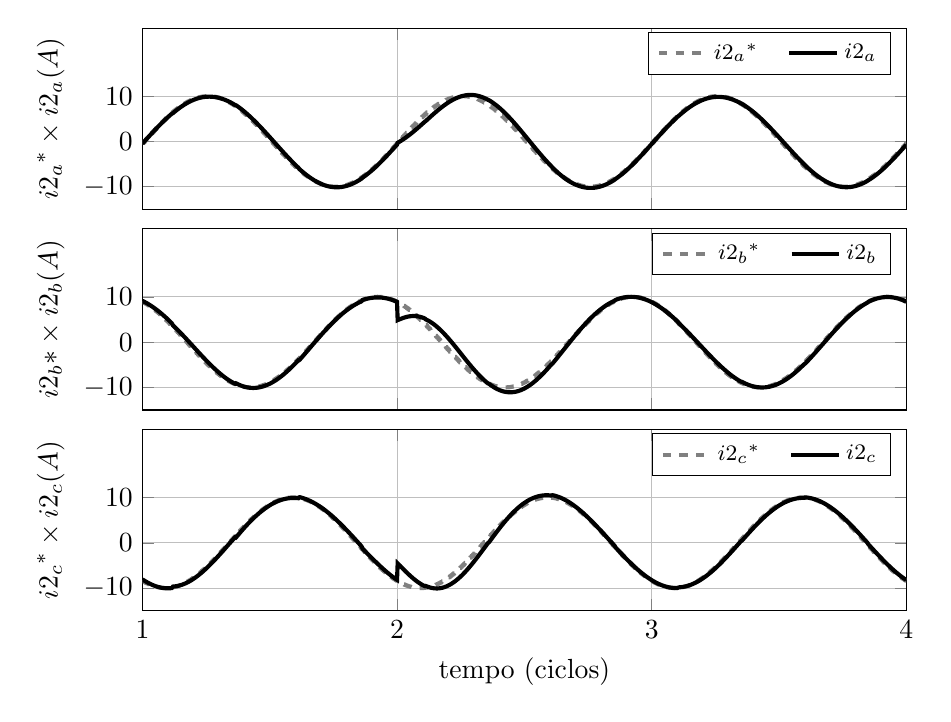
\begin{tikzpicture}

\begin{axis}[%
width=0.8\textwidth,
height=0.189701500343624\textwidth,
scale only axis,
xmin=0.0166666666666667,
xmax=0.0666666666666667,
xtick={0.0166666666666667,0.0333333333333333,0.05,0.0666666666666667},
xticklabels={\empty},
xmajorgrids,
ymin=-15,
ymax=25,
ytick={-10,   0,  10},
ylabel={${\text{i2}_\text{b}}\text{* }\times\text{ i2}_\text{b}\text{ (A)}$},
ymajorgrids,
name=plot2,
legend style={draw=black,fill=white,legend cell align=left},
scaled x ticks = false,
legend columns=-1,
legend style={/tikz/every even column/.append style={column sep=0.3cm}},
legend style={font=\footnotesize}
]
\addplot [color=gray,dashed,line width=1.5pt]
  table[row sep=crcr]{0.0166583333333333	8.95711760239421\\
0.0167	8.81303452065\\
0.0167416666666667	8.81303452065\\
0.0167833333333333	8.66025403784447\\
0.016825	8.66025403784447\\
0.0168666666666667	8.49892692986872\\
0.0169083333333333	8.49892692986872\\
0.01695	8.32921240710107\\
0.0169916666666667	8.32921240710107\\
0.0170333333333333	8.15127795728562\\
0.017075	8.15127795728562\\
0.0171166666666667	7.96529918024204\\
0.0171583333333333	7.96529918024204\\
0.0172	7.77145961456979\\
0.0172416666666667	7.77145961456979\\
0.0172833333333333	7.56995055651764\\
0.017325	7.56995055651764\\
0.0173666666666667	7.36097087119742\\
0.0174083333333333	7.36097087119742\\
0.01745	7.1447267963281\\
0.0174916666666667	7.1447267963281\\
0.0175333333333333	6.92143173870414\\
0.017575	6.92143173870414\\
0.0176166666666667	6.69130606358865\\
0.0176583333333333	6.69130606358865\\
0.0177	6.45457687723957\\
0.0177416666666667	6.45457687723957\\
0.0177833333333333	6.21147780278317\\
0.017825	6.21147780278317\\
0.0178666666666667	5.96224874965622\\
0.0179083333333333	5.96224874965622\\
0.01795	5.70713567684438\\
0.0179916666666667	5.70713567684438\\
0.0180333333333333	5.44639035015033\\
0.018075	5.44639035015033\\
0.0181166666666667	5.18027009373136\\
0.0181583333333333	5.18027009373136\\
0.0182	4.90903753615147\\
0.0182416666666667	4.90903753615147\\
0.0182833333333333	4.63296035119867\\
0.018325	4.63296035119867\\
0.0183666666666667	4.35231099372333\\
0.0184083333333333	4.35231099372333\\
0.01845	4.06736643075805\\
0.0184916666666667	4.06736643075805\\
0.0185333333333333	3.77840786818472\\
0.018575	3.77840786818472\\
0.0186166666666667	3.4857204732182\\
0.0186583333333333	3.4857204732182\\
0.0187	3.18959309298074\\
0.0187416666666667	3.18959309298074\\
0.0187833333333333	2.89031796944476\\
0.018825	2.89031796944476\\
0.0188666666666667	2.58819045102524\\
0.0189083333333333	2.58819045102524\\
0.01895	2.28350870110659\\
0.0189916666666667	2.28350870110659\\
0.0190333333333333	1.97657340379129\\
0.019075	1.97657340379129\\
0.0191166666666667	1.66768746716105\\
0.0191583333333333	1.66768746716105\\
0.0192	1.35715572434307\\
0.0192416666666667	1.35715572434307\\
0.0192833333333333	1.04528463267656\\
0.019325	1.04528463267656\\
0.0193666666666667	0.732381971276336\\
0.0194083333333333	0.732381971276336\\
0.01945	0.418756537292012\\
0.0194916666666667	0.418756537292012\\
0.0195333333333333	0.104717841162471\\
0.019575	0.104717841162471\\
0.0196166666666667	-0.20942419883356\\
0.0196583333333333	-0.20942419883356\\
0.0197	-0.523359562429432\\
0.0197416666666667	-0.523359562429432\\
0.0197833333333333	-0.836778433323152\\
0.019825	-0.836778433323152\\
0.0198666666666667	-1.14937150492867\\
0.0199083333333333	-1.14937150492867\\
0.01995	-1.46083028562412\\
0.0199916666666667	-1.46083028562412\\
0.0200333333333333	-1.77084740319584\\
0.020075	-1.77084740319584\\
0.0201166666666667	-2.0791169081776\\
0.0201583333333333	-2.0791169081776\\
0.0202	-2.38533457578582\\
0.0202416666666667	-2.38533457578582\\
0.0202833333333333	-2.68919820615267\\
0.020325	-2.68919820615267\\
0.0203666666666667	-2.99040792256089\\
0.0204083333333333	-2.99040792256089\\
0.02045	-3.28866646738586\\
0.0204916666666667	-3.28866646738586\\
0.0205333333333333	-3.58367949545303\\
0.020575	-3.58367949545303\\
0.0206166666666667	-3.87515586452106\\
0.0206583333333333	-3.87515586452106\\
0.0207	-4.16280792260405\\
0.0207416666666667	-4.16280792260405\\
0.0207833333333333	-4.44635179184931\\
0.020825	-4.44635179184931\\
0.0208666666666667	-4.72550764869058\\
0.0209083333333333	-4.72550764869058\\
0.02095	-5.00000000000005\\
0.0209916666666667	-5.00000000000005\\
0.0210333333333333	-5.26955795496682\\
0.021075	-5.26955795496682\\
0.0211166666666667	-5.53391549243349\\
0.0211583333333333	-5.53391549243349\\
0.0212	-5.79281172342684\\
0.0212416666666667	-5.79281172342684\\
0.0212833333333333	-6.0459911486238\\
0.021325	-6.0459911486238\\
0.0213666666666667	-6.29320391049844\\
0.0214083333333333	-6.29320391049844\\
0.02145	-6.53420603990112\\
0.0214916666666667	-6.53420603990112\\
0.0215333333333333	-6.76875969682667\\
0.021575	-6.76875969682667\\
0.0216166666666667	-6.99663340513372\\
0.0216583333333333	-6.99663340513372\\
0.0217	-7.2176022809837\\
0.0217416666666667	-7.2176022809837\\
0.0217833333333333	-7.43144825477402\\
0.021825	-7.43144825477402\\
0.0218666666666667	-7.6379602863465\\
0.0219083333333333	-7.6379602863465\\
0.02195	-7.83693457325848\\
0.0219916666666667	-7.83693457325848\\
0.0220333333333333	-8.02817475191123\\
0.022075	-8.02817475191123\\
0.0221166666666667	-8.21149209133713\\
0.0221583333333333	-8.21149209133713\\
0.0222	-8.38670567945433\\
0.0222416666666667	-8.38670567945433\\
0.0222833333333333	-8.55364260160516\\
0.022325	-8.55364260160516\\
0.0223666666666667	-8.71213811120199\\
0.0224083333333333	-8.71213811120199\\
0.02245	-8.86203579231225\\
0.0224916666666667	-8.86203579231225\\
0.0225333333333333	-9.00318771402204\\
0.022575	-9.00318771402204\\
0.0226166666666667	-9.13545457642611\\
0.0226583333333333	-9.13545457642611\\
0.0227	-9.25870584810006\\
0.0227416666666667	-9.25870584810006\\
0.0227833333333333	-9.37281989491902\\
0.022825	-9.37281989491902\\
0.0228666666666667	-9.47768410009597\\
0.0229083333333333	-9.47768410009597\\
0.02295	-9.57319497532079\\
0.0229916666666667	-9.57319497532079\\
0.0230333333333333	-9.6592582628908\\
0.023075	-9.6592582628908\\
0.0231166666666667	-9.73578902873172\\
0.0231583333333333	-9.73578902873172\\
0.0232	-9.80271174621734\\
0.0232416666666667	-9.80271174621734\\
0.0232833333333333	-9.85996037070517\\
0.023325	-9.85996037070517\\
0.0233666666666667	-9.90747840471456\\
0.0234083333333333	-9.90747840471456\\
0.02345	-9.94521895368285\\
0.0234916666666667	-9.94521895368285\\
0.0235333333333333	-9.97314477224471\\
0.023575	-9.97314477224471\\
0.0236166666666667	-9.99122830098871\\
0.0236583333333333	-9.99122830098871\\
0.0237	-9.99945169365525\\
0.0237416666666667	-9.99945169365525\\
0.0237833333333333	-9.99780683474858\\
0.023825	-9.99780683474858\\
0.0238666666666667	-9.98629534754587\\
0.0239083333333333	-9.98629534754587\\
0.02395	-9.96492859249517\\
0.0239916666666667	-9.96492859249517\\
0.0240333333333333	-9.93372765600409\\
0.024075	-9.93372765600409\\
0.0241166666666667	-9.89272332963001\\
0.0241583333333333	-9.89272332963001\\
0.0242	-9.84195607969255\\
0.0242416666666667	-9.84195607969255\\
0.0242833333333333	-9.78147600733818\\
0.024325	-9.78147600733818\\
0.0243666666666667	-9.71134279909649\\
0.0244083333333333	-9.71134279909649\\
0.02445	-9.63162566797671\\
0.0244916666666667	-9.63162566797671\\
0.0245333333333333	-9.5424032851629\\
0.024575	-9.5424032851629\\
0.0246166666666667	-9.44376370237494\\
0.0246583333333333	-9.44376370237494\\
0.0247	-9.33580426497215\\
0.0247416666666667	-9.33580426497215\\
0.0247833333333333	-9.21863151588513\\
0.024825	-9.21863151588513\\
0.0248666666666667	-9.09236109047081\\
0.0249083333333333	-9.09236109047081\\
0.02495	-8.95711760239425\\
0.0249916666666667	-8.95711760239425\\
0.0250333333333333	-8.81303452065005\\
0.025075	-8.81303452065005\\
0.0251166666666667	-8.66025403784451\\
0.0251583333333333	-8.66025403784451\\
0.0252	-8.49892692986876\\
0.0252416666666667	-8.49892692986876\\
0.0252833333333333	-8.32921240710111\\
0.025325	-8.32921240710111\\
0.0253666666666667	-8.15127795728566\\
0.0254083333333333	-8.15127795728566\\
0.02545	-7.96529918024207\\
0.0254916666666667	-7.96529918024207\\
0.0255333333333333	-7.77145961456982\\
0.025575	-7.77145961456982\\
0.0256166666666667	-7.56995055651767\\
0.0256583333333333	-7.56995055651767\\
0.0257	-7.36097087119745\\
0.0257416666666667	-7.36097087119745\\
0.0257833333333333	-7.14472679632814\\
0.025825	-7.14472679632814\\
0.0258666666666667	-6.92143173870417\\
0.0259083333333333	-6.92143173870417\\
0.02595	-6.69130606358868\\
0.0259916666666667	-6.69130606358868\\
0.0260333333333333	-6.4545768772396\\
0.026075	-6.4545768772396\\
0.0261166666666667	-6.2114778027832\\
0.0261583333333333	-6.2114778027832\\
0.0262	-5.96224874965625\\
0.0262416666666667	-5.96224874965625\\
0.0262833333333333	-5.70713567684441\\
0.026325	-5.70713567684441\\
0.0263666666666667	-5.44639035015036\\
0.0264083333333333	-5.44639035015036\\
0.02645	-5.18027009373139\\
0.0264916666666667	-5.18027009373139\\
0.0265333333333333	-4.90903753615149\\
0.026575	-4.90903753615149\\
0.0266166666666667	-4.6329603511987\\
0.0266583333333333	-4.6329603511987\\
0.0267	-4.35231099372335\\
0.0267416666666667	-4.35231099372335\\
0.0267833333333333	-4.06736643075807\\
0.026825	-4.06736643075807\\
0.0268666666666667	-3.77840786818474\\
0.0269083333333333	-3.77840786818474\\
0.02695	-3.48572047321821\\
0.0269916666666667	-3.48572047321821\\
0.0270333333333333	-3.18959309298076\\
0.027075	-3.18959309298076\\
0.0271166666666667	-2.89031796944477\\
0.0271583333333333	-2.89031796944477\\
0.0272	-2.58819045102526\\
0.0272416666666667	-2.58819045102526\\
0.0272833333333333	-2.28350870110661\\
0.027325	-2.28350870110661\\
0.0273666666666667	-1.9765734037913\\
0.0274083333333333	-1.9765734037913\\
0.02745	-1.66768746716106\\
0.0274916666666667	-1.66768746716106\\
0.0275333333333333	-1.35715572434308\\
0.027575	-1.35715572434308\\
0.0276166666666667	-1.04528463267656\\
0.0276583333333333	-1.04528463267656\\
0.0277	-0.732381971276341\\
0.0277416666666667	-0.732381971276341\\
0.0277833333333333	-0.418756537292015\\
0.027825	-0.418756537292015\\
0.0278666666666667	-0.104717841162473\\
0.0279083333333333	-0.104717841162473\\
0.02795	0.209424198833559\\
0.0279916666666667	0.209424198833559\\
0.0280333333333333	0.523359562429433\\
0.028075	0.523359562429433\\
0.0281166666666667	0.836778433323154\\
0.0281583333333333	0.836778433323154\\
0.0282	1.14937150492867\\
0.0282416666666667	1.14937150492867\\
0.0282833333333333	1.46083028562412\\
0.028325	1.46083028562412\\
0.0283666666666667	1.77084740319585\\
0.0284083333333333	1.77084740319585\\
0.02845	2.07911690817761\\
0.0284916666666667	2.07911690817761\\
0.0285333333333333	2.38533457578583\\
0.028575	2.38533457578583\\
0.0286166666666667	2.68919820615268\\
0.0286583333333333	2.68919820615268\\
0.0287	2.9904079225609\\
0.0287416666666667	2.9904079225609\\
0.0287833333333333	3.28866646738587\\
0.028825	3.28866646738587\\
0.0288666666666667	3.58367949545304\\
0.0289083333333333	3.58367949545304\\
0.02895	3.87515586452107\\
0.0289916666666667	3.87515586452107\\
0.0290333333333333	4.16280792260406\\
0.029075	4.16280792260406\\
0.0291166666666667	4.44635179184933\\
0.0291583333333333	4.44635179184933\\
0.0292	4.7255076486906\\
0.0292416666666667	4.7255076486906\\
0.0292833333333333	5.00000000000006\\
0.029325	5.00000000000006\\
0.0293666666666667	5.26955795496684\\
0.0294083333333333	5.26955795496684\\
0.02945	5.53391549243351\\
0.0294916666666667	5.53391549243351\\
0.0295333333333333	5.79281172342686\\
0.029575	5.79281172342686\\
0.0296166666666667	6.04599114862383\\
0.0296583333333333	6.04599114862383\\
0.0297	6.29320391049846\\
0.0297416666666667	6.29320391049846\\
0.0297833333333333	6.53420603990114\\
0.029825	6.53420603990114\\
0.0298666666666667	6.7687596968267\\
0.0299083333333333	6.7687596968267\\
0.02995	6.99663340513375\\
0.0299916666666667	6.99663340513375\\
0.0300333333333333	7.21760228098372\\
0.030075	7.21760228098372\\
0.0301166666666667	7.43144825477405\\
0.0301583333333333	7.43144825477405\\
0.0302	7.63796028634653\\
0.0302416666666667	7.63796028634653\\
0.0302833333333333	7.83693457325851\\
0.030325	7.83693457325851\\
0.0303666666666667	8.02817475191126\\
0.0304083333333333	8.02817475191126\\
0.03045	8.21149209133716\\
0.0304916666666667	8.21149209133716\\
0.0305333333333333	8.38670567945436\\
0.030575	8.38670567945436\\
0.0306166666666667	8.55364260160519\\
0.0306583333333333	8.55364260160519\\
0.0307	8.71213811120203\\
0.0307416666666667	8.71213811120203\\
0.0307833333333333	8.86203579231228\\
0.030825	8.86203579231228\\
0.0308666666666667	9.00318771402207\\
0.0309083333333333	9.00318771402207\\
0.03095	9.13545457642615\\
0.0309916666666667	9.13545457642615\\
0.0310333333333333	9.25870584810009\\
0.031075	9.25870584810009\\
0.0311166666666667	9.37281989491906\\
0.0311583333333333	9.37281989491906\\
0.0312	9.477684100096\\
0.0312416666666667	9.477684100096\\
0.0312833333333333	9.57319497532082\\
0.031325	9.57319497532082\\
0.0313666666666667	9.65925826289084\\
0.0314083333333333	9.65925826289084\\
0.03145	9.73578902873176\\
0.0314916666666667	9.73578902873176\\
0.0315333333333333	9.80271174621738\\
0.031575	9.80271174621738\\
0.0316166666666667	9.85996037070521\\
0.0316583333333333	9.85996037070521\\
0.0317	9.9074784047146\\
0.0317416666666667	9.9074784047146\\
0.0317833333333333	9.94521895368289\\
0.031825	9.94521895368289\\
0.0318666666666667	9.97314477224474\\
0.0319083333333333	9.97314477224474\\
0.03195	9.99122830098875\\
0.0319916666666667	9.99122830098875\\
0.0320333333333333	9.99945169365528\\
0.032075	9.99945169365528\\
0.0321166666666667	9.99780683474862\\
0.0321583333333333	9.99780683474862\\
0.0322	9.98629534754591\\
0.0322416666666667	9.98629534754591\\
0.0322833333333333	9.96492859249521\\
0.032325	9.96492859249521\\
0.0323666666666667	9.93372765600413\\
0.0324083333333333	9.93372765600413\\
0.03245	9.89272332963005\\
0.0324916666666667	9.89272332963005\\
0.0325333333333333	9.84195607969259\\
0.032575	9.84195607969259\\
0.0326166666666667	9.78147600733822\\
0.0326583333333333	9.78147600733822\\
0.0327	9.71134279909653\\
0.0327416666666667	9.71134279909653\\
0.0327833333333333	9.63162566797675\\
0.032825	9.63162566797675\\
0.0328666666666667	9.54240328516294\\
0.0329083333333333	9.54240328516294\\
0.03295	9.44376370237498\\
0.0329916666666667	9.44376370237498\\
0.0330333333333333	9.33580426497218\\
0.033075	9.33580426497218\\
0.0331166666666667	9.21863151588517\\
0.0331583333333333	9.21863151588517\\
0.0332	9.09236109047085\\
0.0332416666666667	9.09236109047085\\
0.0332833333333333	8.95711760239429\\
0.033325	8.95711760239429\\
0.0333666666666667	8.81303452065008\\
0.0334083333333333	8.81303452065008\\
0.03345	8.66025403784455\\
0.0334916666666667	8.66025403784455\\
0.0335333333333333	8.49892692986879\\
0.033575	8.49892692986879\\
0.0336166666666667	8.32921240710115\\
0.0336583333333333	8.32921240710115\\
0.0337	8.15127795728569\\
0.0337416666666667	8.15127795728569\\
0.0337833333333333	7.96529918024211\\
0.033825	7.96529918024211\\
0.0338666666666667	7.77145961456986\\
0.0339083333333333	7.77145961456986\\
0.03395	7.56995055651771\\
0.0339916666666667	7.56995055651771\\
0.0340333333333333	7.36097087119748\\
0.034075	7.36097087119748\\
0.0341166666666667	7.14472679632817\\
0.0341583333333333	7.14472679632817\\
0.0342	6.9214317387042\\
0.0342416666666667	6.9214317387042\\
0.0342833333333333	6.69130606358871\\
0.034325	6.69130606358871\\
0.0343666666666667	6.45457687723963\\
0.0344083333333333	6.45457687723963\\
0.03445	6.21147780278323\\
0.0344916666666667	6.21147780278323\\
0.0345333333333333	5.96224874965628\\
0.034575	5.96224874965628\\
0.0346166666666667	5.70713567684443\\
0.0346583333333333	5.70713567684443\\
0.0347	5.44639035015038\\
0.0347416666666667	5.44639035015038\\
0.0347833333333333	5.18027009373141\\
0.034825	5.18027009373141\\
0.0348666666666667	4.90903753615151\\
0.0349083333333333	4.90903753615151\\
0.03495	4.63296035119872\\
0.0349916666666667	4.63296035119872\\
0.0350333333333333	4.35231099372337\\
0.035075	4.35231099372337\\
0.0351166666666667	4.06736643075809\\
0.0351583333333333	4.06736643075809\\
0.0352	3.77840786818476\\
0.0352416666666667	3.77840786818476\\
0.0352833333333333	3.48572047321823\\
0.035325	3.48572047321823\\
0.0353666666666667	3.18959309298077\\
0.0354083333333333	3.18959309298077\\
0.03545	2.89031796944478\\
0.0354916666666667	2.89031796944478\\
0.0355333333333333	2.58819045102527\\
0.035575	2.58819045102527\\
0.0356166666666667	2.28350870110662\\
0.0356583333333333	2.28350870110662\\
0.0357	1.97657340379131\\
0.0357416666666667	1.97657340379131\\
0.0357833333333333	1.66768746716107\\
0.035825	1.66768746716107\\
0.0358666666666667	1.35715572434309\\
0.0359083333333333	1.35715572434309\\
0.03595	1.04528463267657\\
0.0359916666666667	1.04528463267657\\
0.0360333333333333	0.732381971276348\\
0.036075	0.732381971276348\\
0.0361166666666667	0.418756537292022\\
0.0361583333333333	0.418756537292022\\
0.0362	0.104717841162477\\
0.0362416666666667	0.104717841162477\\
0.0362833333333333	-0.209424198833557\\
0.036325	-0.209424198833557\\
0.0363666666666667	-0.523359562429431\\
0.0364083333333333	-0.523359562429431\\
0.03645	-0.836778433323154\\
0.0364916666666667	-0.836778433323154\\
0.0365333333333333	-1.14937150492867\\
0.036575	-1.14937150492867\\
0.0366166666666667	-1.46083028562413\\
0.0366583333333333	-1.46083028562413\\
0.0367	-1.77084740319585\\
0.0367416666666667	-1.77084740319585\\
0.0367833333333333	-2.07911690817762\\
0.036825	-2.07911690817762\\
0.0368666666666667	-2.38533457578584\\
0.0369083333333333	-2.38533457578584\\
0.03695	-2.68919820615269\\
0.0369916666666667	-2.68919820615269\\
0.0370333333333333	-2.99040792256091\\
0.037075	-2.99040792256091\\
0.0371166666666667	-3.28866646738588\\
0.0371583333333333	-3.28866646738588\\
0.0372	-3.58367949545306\\
0.0372416666666667	-3.58367949545306\\
0.0372833333333333	-3.87515586452109\\
0.037325	-3.87515586452109\\
0.0373666666666667	-4.16280792260408\\
0.0374083333333333	-4.16280792260408\\
0.03745	-4.44635179184934\\
0.0374916666666667	-4.44635179184934\\
0.0375333333333333	-4.72550764869062\\
0.037575	-4.72550764869062\\
0.0376166666666667	-5.00000000000008\\
0.0376583333333333	-5.00000000000008\\
0.0377	-5.26955795496686\\
0.0377416666666667	-5.26955795496686\\
0.0377833333333333	-5.53391549243353\\
0.037825	-5.53391549243353\\
0.0378666666666667	-5.79281172342689\\
0.0379083333333333	-5.79281172342689\\
0.03795	-6.04599114862385\\
0.0379916666666667	-6.04599114862385\\
0.0380333333333333	-6.29320391049848\\
0.038075	-6.29320391049848\\
0.0381166666666667	-6.53420603990117\\
0.0381583333333333	-6.53420603990117\\
0.0382	-6.76875969682673\\
0.0382416666666667	-6.76875969682673\\
0.0382833333333333	-6.99663340513378\\
0.038325	-6.99663340513378\\
0.0383666666666667	-7.21760228098375\\
0.0384083333333333	-7.21760228098375\\
0.03845	-7.43144825477408\\
0.0384916666666667	-7.43144825477408\\
0.0385333333333333	-7.63796028634656\\
0.038575	-7.63796028634656\\
0.0386166666666667	-7.83693457325854\\
0.0386583333333333	-7.83693457325854\\
0.0387	-8.02817475191129\\
0.0387416666666667	-8.02817475191129\\
0.0387833333333333	-8.21149209133719\\
0.038825	-8.21149209133719\\
0.0388666666666667	-8.3867056794544\\
0.0389083333333333	-8.3867056794544\\
0.03895	-8.55364260160523\\
0.0389916666666667	-8.55364260160523\\
0.0390333333333333	-8.71213811120206\\
0.039075	-8.71213811120206\\
0.0391166666666667	-8.86203579231232\\
0.0391583333333333	-8.86203579231232\\
0.0392	-9.00318771402211\\
0.0392416666666667	-9.00318771402211\\
0.0392833333333333	-9.13545457642618\\
0.039325	-9.13545457642618\\
0.0393666666666667	-9.25870584810013\\
0.0394083333333333	-9.25870584810013\\
0.03945	-9.3728198949191\\
0.0394916666666667	-9.3728198949191\\
0.0395333333333333	-9.47768410009604\\
0.039575	-9.47768410009604\\
0.0396166666666667	-9.57319497532086\\
0.0396583333333333	-9.57319497532086\\
0.0397	-9.65925826289087\\
0.0397416666666667	-9.65925826289087\\
0.0397833333333333	-9.7357890287318\\
0.039825	-9.7357890287318\\
0.0398666666666667	-9.80271174621742\\
0.0399083333333333	-9.80271174621742\\
0.03995	-9.85996037070525\\
0.0399916666666667	-9.85996037070525\\
0.0400333333333333	-9.90747840471464\\
0.040075	-9.90747840471464\\
0.0401166666666667	-9.94521895368294\\
0.0401583333333333	-9.94521895368294\\
0.0402	-9.97314477224478\\
0.0402416666666667	-9.97314477224478\\
0.0402833333333333	-9.99122830098879\\
0.040325	-9.99122830098879\\
0.0403666666666667	-9.99945169365533\\
0.0404083333333333	-9.99945169365533\\
0.04045	-9.99780683474866\\
0.0404916666666667	-9.99780683474866\\
0.0405333333333333	-9.98629534754595\\
0.040575	-9.98629534754595\\
0.0406166666666667	-9.96492859249525\\
0.0406583333333333	-9.96492859249525\\
0.0407	-9.93372765600417\\
0.0407416666666667	-9.93372765600417\\
0.0407833333333333	-9.89272332963009\\
0.040825	-9.89272332963009\\
0.0408666666666667	-9.84195607969263\\
0.0409083333333333	-9.84195607969263\\
0.04095	-9.78147600733827\\
0.0409916666666667	-9.78147600733827\\
0.0410333333333333	-9.71134279909657\\
0.041075	-9.71134279909657\\
0.0411166666666667	-9.63162566797679\\
0.0411583333333333	-9.63162566797679\\
0.0412	-9.54240328516298\\
0.0412416666666667	-9.54240328516298\\
0.0412833333333333	-9.44376370237502\\
0.041325	-9.44376370237502\\
0.0413666666666667	-9.33580426497222\\
0.0414083333333333	-9.33580426497222\\
0.04145	-9.21863151588521\\
0.0414916666666667	-9.21863151588521\\
0.0415333333333333	-9.09236109047089\\
0.041575	-9.09236109047089\\
0.0416166666666667	-8.95711760239433\\
0.0416583333333333	-8.95711760239433\\
0.0417	-8.81303452065012\\
0.0417416666666667	-8.81303452065012\\
0.0417833333333333	-8.66025403784458\\
0.041825	-8.66025403784458\\
0.0418666666666667	-8.49892692986883\\
0.0419083333333333	-8.49892692986883\\
0.04195	-8.32921240710118\\
0.0419916666666667	-8.32921240710118\\
0.0420333333333333	-8.15127795728573\\
0.042075	-8.15127795728573\\
0.0421166666666667	-7.96529918024214\\
0.0421583333333333	-7.96529918024214\\
0.0422	-7.77145961456989\\
0.0422416666666667	-7.77145961456989\\
0.0422833333333333	-7.56995055651774\\
0.042325	-7.56995055651774\\
0.0423666666666667	-7.36097087119751\\
0.0424083333333333	-7.36097087119751\\
0.04245	-7.1447267963282\\
0.0424916666666667	-7.1447267963282\\
0.0425333333333333	-6.92143173870423\\
0.042575	-6.92143173870423\\
0.0426166666666667	-6.69130606358874\\
0.0426583333333333	-6.69130606358874\\
0.0427	-6.45457687723966\\
0.0427416666666667	-6.45457687723966\\
0.0427833333333333	-6.21147780278325\\
0.042825	-6.21147780278325\\
0.0428666666666667	-5.9622487496563\\
0.0429083333333333	-5.9622487496563\\
0.04295	-5.70713567684446\\
0.0429916666666667	-5.70713567684446\\
0.0430333333333333	-5.44639035015041\\
0.043075	-5.44639035015041\\
0.0431166666666667	-5.18027009373143\\
0.0431583333333333	-5.18027009373143\\
0.0432	-4.90903753615153\\
0.0432416666666667	-4.90903753615153\\
0.0432833333333333	-4.63296035119874\\
0.043325	-4.63296035119874\\
0.0433666666666667	-4.35231099372339\\
0.0434083333333333	-4.35231099372339\\
0.04345	-4.06736643075811\\
0.0434916666666667	-4.06736643075811\\
0.0435333333333333	-3.77840786818477\\
0.043575	-3.77840786818477\\
0.0436166666666667	-3.48572047321825\\
0.0436583333333333	-3.48572047321825\\
0.0437	-3.18959309298079\\
0.0437416666666667	-3.18959309298079\\
0.0437833333333333	-2.8903179694448\\
0.043825	-2.8903179694448\\
0.0438666666666667	-2.58819045102528\\
0.0439083333333333	-2.58819045102528\\
0.04395	-2.28350870110663\\
0.0439916666666667	-2.28350870110663\\
0.0440333333333333	-1.97657340379133\\
0.044075	-1.97657340379133\\
0.0441166666666667	-1.66768746716108\\
0.0441583333333333	-1.66768746716108\\
0.0442	-1.35715572434309\\
0.0442416666666667	-1.35715572434309\\
0.0442833333333333	-1.04528463267658\\
0.044325	-1.04528463267658\\
0.0443666666666667	-0.732381971276353\\
0.0444083333333333	-0.732381971276353\\
0.04445	-0.418756537292025\\
0.0444916666666667	-0.418756537292025\\
0.0445333333333333	-0.104717841162479\\
0.044575	-0.104717841162479\\
0.0446166666666667	0.209424198833555\\
0.0446583333333333	0.209424198833555\\
0.0447	0.523359562429432\\
0.0447416666666667	0.523359562429432\\
0.0447833333333333	0.836778433323156\\
0.044825	0.836778433323156\\
0.0448666666666667	1.14937150492867\\
0.0449083333333333	1.14937150492867\\
0.04495	1.46083028562413\\
0.0449916666666667	1.46083028562413\\
0.0450333333333333	1.77084740319586\\
0.045075	1.77084740319586\\
0.0451166666666667	2.07911690817762\\
0.0451583333333333	2.07911690817762\\
0.0452	2.38533457578585\\
0.0452416666666667	2.38533457578585\\
0.0452833333333333	2.6891982061527\\
0.045325	2.6891982061527\\
0.0453666666666667	2.99040792256092\\
0.0454083333333333	2.99040792256092\\
0.04545	3.28866646738589\\
0.0454916666666667	3.28866646738589\\
0.0455333333333333	3.58367949545307\\
0.045575	3.58367949545307\\
0.0456166666666667	3.8751558645211\\
0.0456583333333333	3.8751558645211\\
0.0457	4.16280792260409\\
0.0457416666666667	4.16280792260409\\
0.0457833333333333	4.44635179184936\\
0.045825	4.44635179184936\\
0.0458666666666667	4.72550764869064\\
0.0459083333333333	4.72550764869064\\
0.04595	5.0000000000001\\
0.0459916666666667	5.0000000000001\\
0.0460333333333333	5.26955795496689\\
0.046075	5.26955795496689\\
0.0461166666666667	5.53391549243356\\
0.0461583333333333	5.53391549243356\\
0.0462	5.79281172342691\\
0.0462416666666667	5.79281172342691\\
0.0462833333333333	6.04599114862388\\
0.046325	6.04599114862388\\
0.0463666666666667	6.29320391049851\\
0.0464083333333333	6.29320391049851\\
0.04645	6.5342060399012\\
0.0464916666666667	6.5342060399012\\
0.0465333333333333	6.76875969682676\\
0.046575	6.76875969682676\\
0.0466166666666667	6.99663340513381\\
0.0466583333333333	6.99663340513381\\
0.0467	7.21760228098379\\
0.0467416666666667	7.21760228098379\\
0.0467833333333333	7.43144825477411\\
0.046825	7.43144825477411\\
0.0468666666666667	7.6379602863466\\
0.0469083333333333	7.6379602863466\\
0.04695	7.83693457325858\\
0.0469916666666667	7.83693457325858\\
0.0470333333333333	8.02817475191133\\
0.047075	8.02817475191133\\
0.0471166666666667	8.21149209133723\\
0.0471583333333333	8.21149209133723\\
0.0472	8.38670567945444\\
0.0472416666666667	8.38670567945444\\
0.0472833333333333	8.55364260160527\\
0.047325	8.55364260160527\\
0.0473666666666667	8.7121381112021\\
0.0474083333333333	8.7121381112021\\
0.04745	8.86203579231236\\
0.0474916666666667	8.86203579231236\\
0.0475333333333333	9.00318771402215\\
0.047575	9.00318771402215\\
0.0476166666666667	9.13545457642623\\
0.0476583333333333	9.13545457642623\\
0.0477	9.25870584810017\\
0.0477416666666667	9.25870584810017\\
0.0477833333333333	9.37281989491914\\
0.047825	9.37281989491914\\
0.0478666666666667	9.47768410009609\\
0.0479083333333333	9.47768410009609\\
0.04795	9.57319497532091\\
0.0479916666666667	9.57319497532091\\
0.0480333333333333	9.65925826289092\\
0.048075	9.65925826289092\\
0.0481166666666667	9.73578902873184\\
0.0481583333333333	9.73578902873184\\
0.0482	9.80271174621746\\
0.0482416666666667	9.80271174621746\\
0.0482833333333333	9.85996037070529\\
0.048325	9.85996037070529\\
0.0483666666666667	9.90747840471468\\
0.0484083333333333	9.90747840471468\\
0.04845	9.94521895368298\\
0.0484916666666667	9.94521895368298\\
0.0485333333333333	9.97314477224483\\
0.048575	9.97314477224483\\
0.0486166666666667	9.99122830098883\\
0.0486583333333333	9.99122830098883\\
0.0487	9.99945169365537\\
0.0487416666666667	9.99945169365537\\
0.0487833333333333	9.99780683474871\\
0.048825	9.99780683474871\\
0.0488666666666667	9.98629534754599\\
0.0489083333333333	9.98629534754599\\
0.04895	9.9649285924953\\
0.0489916666666667	9.9649285924953\\
0.0490333333333333	9.93372765600422\\
0.049075	9.93372765600422\\
0.0491166666666667	9.89272332963014\\
0.0491583333333333	9.89272332963014\\
0.0492	9.84195607969268\\
0.0492416666666667	9.84195607969268\\
0.0492833333333333	9.78147600733831\\
0.049325	9.78147600733831\\
0.0493666666666667	9.71134279909661\\
0.0494083333333333	9.71134279909661\\
0.04945	9.63162566797684\\
0.0494916666666667	9.63162566797684\\
0.0495333333333333	9.54240328516302\\
0.049575	9.54240328516302\\
0.0496166666666667	9.44376370237506\\
0.0496583333333333	9.44376370237506\\
0.0497	9.33580426497227\\
0.0497416666666667	9.33580426497227\\
0.0497833333333333	9.21863151588525\\
0.049825	9.21863151588525\\
0.0498666666666667	9.09236109047093\\
0.0499083333333333	9.09236109047093\\
0.04995	8.95711760239437\\
0.0499916666666667	8.95711760239437\\
0.0500333333333333	8.81303452065016\\
0.050075	8.81303452065016\\
0.0501166666666667	8.66025403784462\\
0.0501583333333333	8.66025403784462\\
0.0502	8.49892692986887\\
0.0502416666666667	8.49892692986887\\
0.0502833333333333	8.32921240710123\\
0.050325	8.32921240710123\\
0.0503666666666667	8.15127795728577\\
0.0504083333333333	8.15127795728577\\
0.05045	7.96529918024218\\
0.0504916666666667	7.96529918024218\\
0.0505333333333333	7.77145961456993\\
0.050575	7.77145961456993\\
0.0506166666666667	7.56995055651778\\
0.0506583333333333	7.56995055651778\\
0.0507	7.36097087119755\\
0.0507416666666667	7.36097087119755\\
0.0507833333333333	7.14472679632824\\
0.050825	7.14472679632824\\
0.0508666666666667	6.92143173870427\\
0.0509083333333333	6.92143173870427\\
0.05095	6.69130606358878\\
0.0509916666666667	6.69130606358878\\
0.0510333333333333	6.45457687723969\\
0.051075	6.45457687723969\\
0.0511166666666667	6.21147780278329\\
0.0511583333333333	6.21147780278329\\
0.0512	5.96224874965633\\
0.0512416666666667	5.96224874965633\\
0.0512833333333333	5.70713567684449\\
0.051325	5.70713567684449\\
0.0513666666666667	5.44639035015043\\
0.0514083333333333	5.44639035015043\\
0.05145	5.18027009373146\\
0.0514916666666667	5.18027009373146\\
0.0515333333333333	4.90903753615156\\
0.051575	4.90903753615156\\
0.0516166666666667	4.63296035119876\\
0.0516583333333333	4.63296035119876\\
0.0517	4.35231099372341\\
0.0517416666666667	4.35231099372341\\
0.0517833333333333	4.06736643075813\\
0.051825	4.06736643075813\\
0.0518666666666667	3.77840786818479\\
0.0519083333333333	3.77840786818479\\
0.05195	3.48572047321827\\
0.0519916666666667	3.48572047321827\\
0.0520333333333333	3.18959309298081\\
0.052075	3.18959309298081\\
0.0521166666666667	2.89031796944481\\
0.0521583333333333	2.89031796944481\\
0.0522	2.5881904510253\\
0.0522416666666667	2.5881904510253\\
0.0522833333333333	2.28350870110664\\
0.052325	2.28350870110664\\
0.0523666666666667	1.97657340379134\\
0.0524083333333333	1.97657340379134\\
0.05245	1.66768746716109\\
0.0524916666666667	1.66768746716109\\
0.0525333333333333	1.3571557243431\\
0.052575	1.3571557243431\\
0.0526166666666667	1.04528463267659\\
0.0526583333333333	1.04528463267659\\
0.0527	0.73238197127636\\
0.0527416666666667	0.73238197127636\\
0.0527833333333333	0.418756537292029\\
0.052825	0.418756537292029\\
0.0528666666666667	0.104717841162482\\
0.0529083333333333	0.104717841162482\\
0.05295	-0.209424198833554\\
0.0529916666666667	-0.209424198833554\\
0.0530333333333333	-0.523359562429432\\
0.053075	-0.523359562429432\\
0.0531166666666667	-0.836778433323157\\
0.0531583333333333	-0.836778433323157\\
0.0532	-1.14937150492868\\
0.0532416666666667	-1.14937150492868\\
0.0532833333333333	-1.46083028562414\\
0.053325	-1.46083028562414\\
0.0533666666666667	-1.77084740319586\\
0.0534083333333333	-1.77084740319586\\
0.05345	-2.07911690817763\\
0.0534916666666667	-2.07911690817763\\
0.0535333333333333	-2.38533457578585\\
0.053575	-2.38533457578585\\
0.0536166666666667	-2.68919820615271\\
0.0536583333333333	-2.68919820615271\\
0.0537	-2.99040792256093\\
0.0537416666666667	-2.99040792256093\\
0.0537833333333333	-3.2886664673859\\
0.053825	-3.2886664673859\\
0.0538666666666667	-3.58367949545308\\
0.0539083333333333	-3.58367949545308\\
0.05395	-3.87515586452112\\
0.0539916666666667	-3.87515586452112\\
0.0540333333333333	-4.16280792260411\\
0.054075	-4.16280792260411\\
0.0541166666666667	-4.44635179184938\\
0.0541583333333333	-4.44635179184938\\
0.0542	-4.72550764869065\\
0.0542416666666667	-4.72550764869065\\
0.0542833333333333	-5.00000000000012\\
0.054325	-5.00000000000012\\
0.0543666666666667	-5.26955795496691\\
0.0544083333333333	-5.26955795496691\\
0.05445	-5.53391549243358\\
0.0544916666666667	-5.53391549243358\\
0.0545333333333333	-5.79281172342693\\
0.054575	-5.79281172342693\\
0.0546166666666667	-6.0459911486239\\
0.0546583333333333	-6.0459911486239\\
0.0547	-6.29320391049854\\
0.0547416666666667	-6.29320391049854\\
0.0547833333333333	-6.53420603990122\\
0.054825	-6.53420603990122\\
0.0548666666666667	-6.76875969682678\\
0.0549083333333333	-6.76875969682678\\
0.05495	-6.99663340513384\\
0.0549916666666667	-6.99663340513384\\
0.0550333333333333	-7.21760228098381\\
0.055075	-7.21760228098381\\
0.0551166666666667	-7.43144825477414\\
0.0551583333333333	-7.43144825477414\\
0.0552	-7.63796028634663\\
0.0552416666666667	-7.63796028634663\\
0.0552833333333333	-7.83693457325861\\
0.055325	-7.83693457325861\\
0.0553666666666667	-8.02817475191136\\
0.0554083333333333	-8.02817475191136\\
0.05545	-8.21149209133726\\
0.0554916666666667	-8.21149209133726\\
0.0555333333333333	-8.38670567945447\\
0.055575	-8.38670567945447\\
0.0556166666666667	-8.5536426016053\\
0.0556583333333333	-8.5536426016053\\
0.0557	-8.71213811120214\\
0.0557416666666667	-8.71213811120214\\
0.0557833333333333	-8.86203579231239\\
0.055825	-8.86203579231239\\
0.0558666666666667	-9.00318771402219\\
0.0559083333333333	-9.00318771402219\\
0.05595	-9.13545457642627\\
0.0559916666666667	-9.13545457642627\\
0.0560333333333333	-9.25870584810021\\
0.056075	-9.25870584810021\\
0.0561166666666667	-9.37281989491918\\
0.0561583333333333	-9.37281989491918\\
0.0562	-9.47768410009613\\
0.0562416666666667	-9.47768410009613\\
0.0562833333333333	-9.57319497532095\\
0.056325	-9.57319497532095\\
0.0563666666666667	-9.65925826289096\\
0.0564083333333333	-9.65925826289096\\
0.05645	-9.73578902873188\\
0.0564916666666667	-9.73578902873188\\
0.0565333333333333	-9.8027117462175\\
0.056575	-9.8027117462175\\
0.0566166666666667	-9.85996037070534\\
0.0566583333333333	-9.85996037070534\\
0.0567	-9.90747840471473\\
0.0567416666666667	-9.90747840471473\\
0.0567833333333333	-9.94521895368302\\
0.056825	-9.94521895368302\\
0.0568666666666667	-9.97314477224487\\
0.0569083333333333	-9.97314477224487\\
0.05695	-9.99122830098888\\
0.0569916666666667	-9.99122830098888\\
0.0570333333333333	-9.99945169365542\\
0.057075	-9.99945169365542\\
0.0571166666666667	-9.99780683474875\\
0.0571583333333333	-9.99780683474875\\
0.0572	-9.98629534754604\\
0.0572416666666667	-9.98629534754604\\
0.0572833333333333	-9.96492859249534\\
0.057325	-9.96492859249534\\
0.0573666666666667	-9.93372765600427\\
0.0574083333333333	-9.93372765600427\\
0.05745	-9.89272332963018\\
0.0574916666666667	-9.89272332963018\\
0.0575333333333333	-9.84195607969272\\
0.057575	-9.84195607969272\\
0.0576166666666667	-9.78147600733836\\
0.0576583333333333	-9.78147600733836\\
0.0577	-9.71134279909666\\
0.0577416666666667	-9.71134279909666\\
0.0577833333333333	-9.63162566797688\\
0.057825	-9.63162566797688\\
0.0578666666666667	-9.54240328516306\\
0.0579083333333333	-9.54240328516306\\
0.05795	-9.44376370237511\\
0.0579916666666667	-9.44376370237511\\
0.0580333333333333	-9.33580426497231\\
0.058075	-9.33580426497231\\
0.0581166666666667	-9.21863151588529\\
0.0581583333333333	-9.21863151588529\\
0.0582	-9.09236109047097\\
0.0582416666666667	-9.09236109047097\\
0.0582833333333333	-8.95711760239441\\
0.058325	-8.95711760239441\\
0.0583666666666667	-8.8130345206502\\
0.0584083333333333	-8.8130345206502\\
0.05845	-8.66025403784466\\
0.0584916666666667	-8.66025403784466\\
0.0585333333333333	-8.49892692986891\\
0.058575	-8.49892692986891\\
0.0586166666666667	-8.32921240710126\\
0.0586583333333333	-8.32921240710126\\
0.0587	-8.1512779572858\\
0.0587416666666667	-8.1512779572858\\
0.0587833333333333	-7.96529918024222\\
0.058825	-7.96529918024222\\
0.0588666666666667	-7.77145961456996\\
0.0589083333333333	-7.77145961456996\\
0.05895	-7.56995055651781\\
0.0589916666666667	-7.56995055651781\\
0.0590333333333333	-7.36097087119758\\
0.059075	-7.36097087119758\\
0.0591166666666667	-7.14472679632827\\
0.0591583333333333	-7.14472679632827\\
0.0592	-6.9214317387043\\
0.0592416666666667	-6.9214317387043\\
0.0592833333333333	-6.69130606358881\\
0.059325	-6.69130606358881\\
0.0593666666666667	-6.45457687723972\\
0.0594083333333333	-6.45457687723972\\
0.05945	-6.21147780278331\\
0.0594916666666667	-6.21147780278331\\
0.0595333333333333	-5.96224874965636\\
0.059575	-5.96224874965636\\
0.0596166666666667	-5.70713567684451\\
0.0596583333333333	-5.70713567684451\\
0.0597	-5.44639035015046\\
0.0597416666666667	-5.44639035015046\\
0.0597833333333333	-5.18027009373148\\
0.059825	-5.18027009373148\\
0.0598666666666667	-4.90903753615158\\
0.0599083333333333	-4.90903753615158\\
0.05995	-4.63296035119878\\
0.0599916666666667	-4.63296035119878\\
0.0600333333333333	-4.35231099372343\\
0.060075	-4.35231099372343\\
0.0601166666666667	-4.06736643075815\\
0.0601583333333333	-4.06736643075815\\
0.0602	-3.77840786818481\\
0.0602416666666667	-3.77840786818481\\
0.0602833333333333	-3.48572047321828\\
0.060325	-3.48572047321828\\
0.0603666666666667	-3.18959309298082\\
0.0604083333333333	-3.18959309298082\\
0.06045	-2.89031796944483\\
0.0604916666666667	-2.89031796944483\\
0.0605333333333333	-2.58819045102531\\
0.060575	-2.58819045102531\\
0.0606166666666667	-2.28350870110665\\
0.0606583333333333	-2.28350870110665\\
0.0607	-1.97657340379135\\
0.0607416666666667	-1.97657340379135\\
0.0607833333333333	-1.6676874671611\\
0.060825	-1.6676874671611\\
0.0608666666666667	-1.35715572434311\\
0.0609083333333333	-1.35715572434311\\
0.06095	-1.04528463267659\\
0.0609916666666667	-1.04528463267659\\
0.0610333333333333	-0.732381971276366\\
0.061075	-0.732381971276366\\
0.0611166666666667	-0.418756537292034\\
0.0611583333333333	-0.418756537292034\\
0.0612	-0.104717841162486\\
0.0612416666666667	-0.104717841162486\\
0.0612833333333333	0.209424198833552\\
0.061325	0.209424198833552\\
0.0613666666666667	0.52335956242943\\
0.0614083333333333	0.52335956242943\\
0.06145	0.836778433323157\\
0.0614916666666667	0.836778433323157\\
0.0615333333333333	1.14937150492868\\
0.061575	1.14937150492868\\
0.0616166666666667	1.46083028562414\\
0.0616583333333333	1.46083028562414\\
0.0617	1.77084740319587\\
0.0617416666666667	1.77084740319587\\
0.0617833333333333	2.07911690817764\\
0.061825	2.07911690817764\\
0.0618666666666667	2.38533457578586\\
0.0619083333333333	2.38533457578586\\
0.06195	2.68919820615272\\
0.0619916666666667	2.68919820615272\\
0.0620333333333333	2.99040792256094\\
0.062075	2.99040792256094\\
0.0621166666666667	3.28866646738591\\
0.0621583333333333	3.28866646738591\\
0.0622	3.5836794954531\\
0.0622416666666667	3.5836794954531\\
0.0622833333333333	3.87515586452113\\
0.062325	3.87515586452113\\
0.0623666666666667	4.16280792260412\\
0.0624083333333333	4.16280792260412\\
0.06245	4.4463517918494\\
0.0624916666666667	4.4463517918494\\
0.0625333333333333	4.72550764869067\\
0.062575	4.72550764869067\\
0.0626166666666667	5.00000000000014\\
0.0626583333333333	5.00000000000014\\
0.0627	5.26955795496693\\
0.0627416666666667	5.26955795496693\\
0.0627833333333333	5.5339154924336\\
0.062825	5.5339154924336\\
0.0628666666666667	5.79281172342696\\
0.0629083333333333	5.79281172342696\\
0.06295	6.04599114862392\\
0.0629916666666667	6.04599114862392\\
0.0630333333333333	6.29320391049856\\
0.063075	6.29320391049856\\
0.0631166666666667	6.53420603990125\\
0.0631583333333333	6.53420603990125\\
0.0632	6.76875969682681\\
0.0632416666666667	6.76875969682681\\
0.0632833333333333	6.99663340513387\\
0.063325	6.99663340513387\\
0.0633666666666667	7.21760228098384\\
0.0634083333333333	7.21760228098384\\
0.06345	7.43144825477417\\
0.0634916666666667	7.43144825477417\\
0.0635333333333333	7.63796028634666\\
0.063575	7.63796028634666\\
0.0636166666666667	7.83693457325864\\
0.0636583333333333	7.83693457325864\\
0.0637	8.0281747519114\\
0.0637416666666667	8.0281747519114\\
0.0637833333333333	8.2114920913373\\
0.063825	8.2114920913373\\
0.0638666666666667	8.3867056794545\\
0.0639083333333333	8.3867056794545\\
0.06395	8.55364260160534\\
0.0639916666666667	8.55364260160534\\
0.0640333333333333	8.71213811120217\\
0.064075	8.71213811120217\\
0.0641166666666667	8.86203579231243\\
0.0641583333333333	8.86203579231243\\
0.0642	9.00318771402222\\
0.0642416666666667	9.00318771402222\\
0.0642833333333333	9.1354545764263\\
0.064325	9.1354545764263\\
0.0643666666666667	9.25870584810025\\
0.0644083333333333	9.25870584810025\\
0.06445	9.37281989491922\\
0.0644916666666667	9.37281989491922\\
0.0645333333333333	9.47768410009616\\
0.064575	9.47768410009616\\
0.0646166666666667	9.57319497532098\\
0.0646583333333333	9.57319497532098\\
0.0647	9.659258262891\\
0.0647416666666667	9.659258262891\\
0.0647833333333333	9.73578902873192\\
0.064825	9.73578902873192\\
0.0648666666666667	9.80271174621754\\
0.0649083333333333	9.80271174621754\\
0.06495	9.85996037070537\\
0.0649916666666667	9.85996037070537\\
0.0650333333333333	9.90747840471476\\
0.065075	9.90747840471476\\
0.0651166666666667	9.94521895368306\\
0.0651583333333333	9.94521895368306\\
0.0652	9.97314477224491\\
0.0652416666666667	9.97314477224491\\
0.0652833333333333	9.99122830098892\\
0.065325	9.99122830098892\\
0.0653666666666667	9.99945169365546\\
0.0654083333333333	9.99945169365546\\
0.06545	9.99780683474879\\
0.0654916666666667	9.99780683474879\\
0.0655333333333333	9.98629534754607\\
0.065575	9.98629534754607\\
0.0656166666666667	9.96492859249538\\
0.0656583333333333	9.96492859249538\\
0.0657	9.9337276560043\\
0.0657416666666667	9.9337276560043\\
0.0657833333333333	9.89272332963022\\
0.065825	9.89272332963022\\
0.0658666666666667	9.84195607969276\\
0.0659083333333333	9.84195607969276\\
0.06595	9.78147600733839\\
0.0659916666666667	9.78147600733839\\
0.0660333333333333	9.71134279909669\\
0.066075	9.71134279909669\\
0.0661166666666667	9.63162566797691\\
0.0661583333333333	9.63162566797691\\
0.0662	9.5424032851631\\
0.0662416666666667	9.5424032851631\\
0.0662833333333333	9.44376370237514\\
0.066325	9.44376370237514\\
0.0663666666666667	9.33580426497234\\
0.0664083333333333	9.33580426497234\\
0.06645	9.21863151588533\\
0.0664916666666667	9.21863151588533\\
0.0665333333333333	9.092361090471\\
0.066575	9.092361090471\\
0.0666166666666667	8.95711760239444\\
0.0666583333333333	8.95711760239444\\
};
\addlegendentry{${\text{i2}_\text{b}}^\text{*}$};

\addplot [color=black,solid,line width=1.5pt]
  table[row sep=crcr]{0.0166583333333333	9.10238729436972\\
0.0167	9.03402165826534\\
0.0167416666666667	8.96368598655141\\
0.0167833333333333	8.89133568061203\\
0.016825	8.81704993622876\\
0.0168666666666667	8.74079343507884\\
0.0169083333333333	8.66265295711749\\
0.01695	8.58259781627092\\
0.0169916666666667	8.50071754137033\\
0.0170333333333333	8.41698140145812\\
0.017075	8.33147777016323\\
0.0171166666666667	8.24417239647427\\
0.0171583333333333	8.15515004140646\\
0.0172	8.06437114911801\\
0.0172416666666667	7.97191608287754\\
0.0172833333333333	7.8777397886972\\
0.017325	7.7819187867049\\
0.0173666666666667	7.68440342410503\\
0.0174083333333333	7.58526770699698\\
0.01745	7.48445879295424\\
0.0174916666666667	7.38204974177135\\
0.0175333333333333	7.27798597031744\\
0.017575	7.1723588885292\\
0.0176166666666667	7.06511633678431\\
0.0176583333333333	6.95626978050029\\
0.0177	6.84580684667755\\
0.0177416666666667	6.73380549079232\\
0.0177833333333333	6.62021165288726\\
0.017825	6.50510560395105\\
0.0178666666666667	6.38843437691671\\
0.0179083333333333	6.2702810790216\\
0.01795	6.15059383602935\\
0.0179916666666667	6.02945861112754\\
0.0180333333333333	5.9068245245065\\
0.018075	5.78278034407908\\
0.0181166666666667	5.65727605146901\\
0.0181583333333333	5.53040314356191\\
0.0182	5.40211233541475\\
0.0182416666666667	5.27249778086378\\
0.0182833333333333	5.14151082265956\\
0.018325	5.00924821301577\\
0.0183666666666667	4.87566184068634\\
0.0184083333333333	4.74085100951404\\
0.01845	4.60476809055667\\
0.0184916666666667	4.46751489796481\\
0.0185333333333333	4.32904423117766\\
0.018575	4.1894603719659\\
0.0186166666666667	3.95920493855525\\
0.0186583333333333	3.68981019134787\\
0.0187	3.55459438762532\\
0.0187416666666667	3.41994135779203\\
0.0187833333333333	3.284551150892\\
0.018825	3.14840956068264\\
0.0188666666666667	3.01131770702737\\
0.0189083333333333	2.87329876433044\\
0.01895	2.73422375637314\\
0.0189916666666667	2.59416394011585\\
0.0190333333333333	2.45303513633463\\
0.019075	2.31093742969384\\
0.0191166666666667	2.16781280767052\\
0.0191583333333333	2.02377684219615\\
0.0192	1.87878453430694\\
0.0192416666666667	1.73295860389567\\
0.0192833333333333	1.58625899975514\\
0.019325	1.43881119869898\\
0.0193666666666667	1.29057586425682\\
0.0194083333333333	1.14167948532007\\
0.01945	0.992081703949671\\
0.0194916666666667	0.841909769593364\\
0.0195333333333333	0.691121953346188\\
0.019575	0.539846655564751\\
0.0196166666666667	0.388041029571302\\
0.0196583333333333	0.235780957939821\\
0.0197	0.0831137819522103\\
0.0197416666666667	-0.0698428576316909\\
0.0197833333333333	-0.223155234126428\\
0.019825	-0.376689340170496\\
0.0198666666666667	-0.530489508286105\\
0.0199083333333333	-0.684419603756233\\
0.01995	-0.838524258952192\\
0.0199916666666667	-0.992665526242936\\
0.0200333333333333	-1.14688842282822\\
0.020075	-1.30105355347543\\
0.0201166666666667	-1.45520644787935\\
0.0201583333333333	-1.60920663242736\\
0.0202	-1.7631002680197\\
0.0202416666666667	-1.91674613701216\\
0.0202833333333333	-2.07019111926222\\
0.020325	-2.22329353670832\\
0.0203666666666667	-2.37610103952102\\
0.0204083333333333	-2.52847172237396\\
0.02045	-2.68045402642318\\
0.0204916666666667	-2.83190601073707\\
0.0205333333333333	-2.98287690775002\\
0.020575	-3.13322490271858\\
0.0206166666666667	-3.28300000950168\\
0.0206583333333333	-3.43206068203698\\
0.0207	-3.58023257831695\\
0.0207416666666667	-3.7277092334411\\
0.0207833333333333	-3.8745094495467\\
0.020825	-4.02042104637285\\
0.0208666666666667	-4.16549853373004\\
0.0209083333333333	-4.30960748092213\\
0.02095	-4.45281035993282\\
0.0209916666666667	-4.59498130928033\\
0.0210333333333333	-4.73619019464951\\
0.021075	-4.87631621588383\\
0.0211166666666667	-5.01543181083388\\
0.0211583333333333	-5.15341682461041\\
0.0212	-5.29034220696768\\
0.0212416666666667	-5.426085096601\\
0.0212833333333333	-5.56071222059019\\
0.021325	-5.6940962192604\\
0.0213666666666667	-5.82629850539151\\
0.0214083333333333	-5.95718699185082\\
0.02145	-6.08681807174369\\
0.0214916666666667	-6.21505582977236\\
0.0215333333333333	-6.34195278597919\\
0.021575	-6.4673706655078\\
0.0216166666666667	-6.59135957583495\\
0.0216583333333333	-6.71378044678016\\
0.0217	-6.83468524636737\\
0.0217416666666667	-6.95399217938414\\
0.0217833333333333	-7.07162840913448\\
0.021825	-7.18751402421548\\
0.0218666666666667	-7.30170428968836\\
0.0219083333333333	-7.4140646101137\\
0.02195	-7.52464610549204\\
0.0219916666666667	-7.6333168162301\\
0.0220333333333333	-7.74012919995476\\
0.022075	-7.84495413606052\\
0.0221166666666667	-7.94784540294816\\
0.0221583333333333	-8.04867680302019\\
0.0222	-8.14750333773792\\
0.0222416666666667	-8.24420176720482\\
0.0222833333333333	-8.33882819422802\\
0.022325	-8.43126236325755\\
0.0223666666666667	-8.52156136312858\\
0.0224083333333333	-8.60960796183905\\
0.02245	-8.69546013657608\\
0.0224916666666667	-8.77900373523377\\
0.0225333333333333	-8.86029754231411\\
0.022575	-8.93923055494087\\
0.0226166666666667	-9.0158622940634\\
0.0226583333333333	-9.09008498121201\\
0.0227	-9.1619588058232\\
0.0227416666666667	-9.21081573522\\
0.0227833333333333	-9.0984668685434\\
0.022825	-9.15855337492306\\
0.0228666666666667	-9.22947523354302\\
0.0229083333333333	-9.29819015157014\\
0.02295	-9.36464137946829\\
0.0229916666666667	-9.42861378862864\\
0.0230333333333333	-9.4900453851335\\
0.023075	-9.54876390071828\\
0.0231166666666667	-9.60476742762568\\
0.0231583333333333	-9.65793002398938\\
0.0232	-9.70828718453498\\
0.0232416666666667	-9.7557417725555\\
0.0232833333333333	-9.80035019237776\\
0.023325	-9.84203175689098\\
0.0233666666666667	-9.88085243770552\\
0.0234083333333333	-9.91674024993253\\
0.02345	-9.94976400939473\\
0.0234916666666667	-9.97985634821345\\
0.0235333333333333	-10.0070856173288\\
0.023575	-10.0313874481953\\
0.0236166666666667	-10.0528285835685\\
0.0236583333333333	-10.0713474398235\\
0.0237	-10.087009152455\\
0.0237416666666667	-10.0997553242113\\
0.0237833333333333	-10.1096212768965\\
0.023825	-10.1165549780692\\
0.0238666666666667	-10.1207046835537\\
0.0239083333333333	-10.1219620846997\\
0.02395	-10.1203887350907\\
0.0239916666666667	-10.1159383416511\\
0.0240333333333333	-10.108673385745\\
0.024075	-10.0985519776893\\
0.0241166666666667	-10.0856362616203\\
0.0241583333333333	-10.0698886487835\\
0.0242	-10.0513707563433\\
0.0242416666666667	-10.0300491222447\\
0.0242833333333333	-10.0059846094998\\
0.024325	-9.97914771255928\\
0.0243666666666667	-9.94959832122408\\
0.0244083333333333	-9.91731074942411\\
0.02445	-9.88234372724823\\
0.0244916666666667	-9.84467529451614\\
0.0245333333333333	-9.80436287400011\\
0.024575	-9.76138817764229\\
0.0246166666666667	-9.71580720736102\\
0.0246583333333333	-9.66760532286042\\
0.0247	-9.61683701630429\\
0.0247416666666667	-9.56349128839865\\
0.0247833333333333	-9.50762104775379\\
0.024825	-9.44931901487656\\
0.0248666666666667	-9.38863375961779\\
0.0249083333333333	-9.32530954504734\\
0.02495	-9.25954240579891\\
0.0249916666666667	-9.19133428032041\\
0.0250333333333333	-9.12072866075138\\
0.025075	-9.0477213069644\\
0.0251166666666667	-8.97234645727584\\
0.0251583333333333	-8.8945965624705\\
0.0252	-8.81449915043002\\
0.0252416666666667	-8.73204780656025\\
0.0252833333333333	-8.64726779224821\\
0.025325	-8.56015786213606\\
0.0253666666666667	-8.47074449149494\\
0.0254083333333333	-8.37903445036129\\
0.02545	-8.28505746633374\\
0.0254916666666667	-8.18882959610245\\
0.0255333333333333	-8.09038431584565\\
0.025575	-7.98974683729511\\
0.0256166666666667	-7.8869537101997\\
0.0256583333333333	-7.78203825639882\\
0.0257	-7.67503879052939\\
0.0257416666666667	-7.56599531459094\\
0.0257833333333333	-7.4549464461354\\
0.025825	-7.34193745850652\\
0.0258666666666667	-7.22694839894464\\
0.0259083333333333	-7.11012337980954\\
0.02595	-6.99148702983552\\
0.0259916666666667	-6.871066065311\\
0.0260333333333333	-6.74889334302512\\
0.026075	-6.6250242807278\\
0.0261166666666667	-6.49948893121508\\
0.0261583333333333	-6.37234524011466\\
0.0262	-6.24362019708288\\
0.0262416666666667	-6.11337417903073\\
0.0262833333333333	-5.98163110846722\\
0.026325	-5.84845377190004\\
0.0263666666666667	-5.71386307769823\\
0.0264083333333333	-5.57792422743959\\
0.02645	-5.44065518096032\\
0.0264916666666667	-5.30212355465025\\
0.0265333333333333	-5.16234441546605\\
0.026575	-5.02138777484591\\
0.0266166666666667	-4.87926584633126\\
0.0266583333333333	-4.73605099633701\\
0.0267	-4.59175261144144\\
0.0267416666666667	-4.44644535816739\\
0.0267833333333333	-4.30013581630143\\
0.026825	-4.15290088980286\\
0.0268666666666667	-4.00645132217426\\
0.0269083333333333	-4.00941990874226\\
0.02695	-3.90500866602108\\
0.0269916666666667	-3.7463128418275\\
0.0270333333333333	-3.58617730564843\\
0.027075	-3.42515227885231\\
0.0271166666666667	-3.26336001143087\\
0.0271583333333333	-3.10098116111065\\
0.0272	-2.93808952673461\\
0.0272416666666667	-2.77482587402537\\
0.0272833333333333	-2.61122185555184\\
0.027325	-2.44739188124668\\
0.0273666666666667	-2.28334165434491\\
0.0274083333333333	-2.11917164363188\\
0.02745	-1.95487269182209\\
0.0274916666666667	-1.79053931585367\\
0.0275333333333333	-1.6261543368841\\
0.027575	-1.4618108533529\\
0.0276166666666667	-1.29748734777055\\
0.0276583333333333	-1.13327765870239\\
0.0277	-0.969157568289885\\
0.0277416666666667	-0.805222391523657\\
0.0277833333333333	-0.641445704083668\\
0.027825	-0.477924319106184\\
0.0278666666666667	-0.314629584722561\\
0.0279083333333333	-0.151666910444537\\
0.02795	0.010929802302895\\
0.0279916666666667	0.173209663659246\\
0.0280333333333333	0.33514019087048\\
0.028075	0.496611559876445\\
0.0281166666666667	0.657659711941593\\
0.0281583333333333	0.81818389481377\\
0.0282	0.978222468495446\\
0.0282416666666667	1.13767393946308\\
0.0282833333333333	1.29657892292822\\
0.028325	1.45483512926401\\
0.0283666666666667	1.61248520279227\\
0.0284083333333333	1.76942599324087\\
0.02845	1.92570195915175\\
0.0284916666666667	2.08120905361234\\
0.0285333333333333	2.23599336371434\\
0.028575	2.38994994741015\\
0.0286166666666667	2.54312636983508\\
0.0286583333333333	2.69541683114933\\
0.0287	2.84687025538406\\
0.0287416666666667	2.99738005024818\\
0.0287833333333333	3.14699640262514\\
0.028825	3.29561201161392\\
0.0288666666666667	3.44327824526797\\
0.0289083333333333	3.58988718809843\\
0.02895	3.73551543356872\\
0.0289916666666667	3.88022294753529\\
0.0290333333333333	4.0237160642344\\
0.029075	4.16601428047325\\
0.0291166666666667	4.30719310890089\\
0.0291583333333333	4.44714029176902\\
0.0292	4.58590489909048\\
0.0292416666666667	4.72336748139296\\
0.0292833333333333	4.85957088335718\\
0.029325	4.99439015782883\\
0.0293666666666667	5.12786580548552\\
0.0294083333333333	5.25987189068068\\
0.02945	5.390450555846\\
0.0294916666666667	5.51947855033307\\
0.0295333333333333	5.64700257484299\\
0.029575	5.77290442675759\\
0.0296166666666667	5.89723678731403\\
0.0296583333333333	6.01988736030132\\
0.0297	6.14091482373526\\
0.0297416666666667	6.26021244138693\\
0.0297833333333333	6.37784394222441\\
0.029825	6.49370710499595\\
0.0298666666666667	6.60786931993153\\
0.0299083333333333	6.72023161624922\\
0.02995	6.83086362928892\\
0.0299916666666667	6.93963550745553\\
0.0300333333333333	7.04662878351116\\
0.030075	7.15182932488549\\
0.0301166666666667	7.25525083871217\\
0.0301583333333333	7.3567961627066\\
0.0302	7.45653575525793\\
0.0302416666666667	7.55437509131568\\
0.0302833333333333	7.65038396578806\\
0.030325	7.74446827210866\\
0.0303666666666667	7.83669703399376\\
0.0304083333333333	7.92697665933048\\
0.03045	8.01537537149727\\
0.0304916666666667	8.10180024444722\\
0.0305333333333333	8.18631870854669\\
0.030575	8.26883867045199\\
0.0306166666666667	8.3494267761454\\
0.0306583333333333	8.42799192122998\\
0.0307	8.5045999613117\\
0.0307416666666667	8.5791609183048\\
0.0307833333333333	8.6517398345412\\
0.030825	8.72224797849278\\
0.0308666666666667	8.79074954415319\\
0.0309083333333333	8.85715715572968\\
0.03095	8.92153411839134\\
0.0309916666666667	8.98379451656429\\
0.0310333333333333	9.1290440832615\\
0.031075	9.29288833989201\\
0.0311166666666667	9.34457768933054\\
0.0311583333333333	9.39000247520132\\
0.0312	9.43306750809908\\
0.0312416666666667	9.47381701559835\\
0.0312833333333333	9.51243794000615\\
0.031325	9.54893851207278\\
0.0313666666666667	9.58344575890155\\
0.0314083333333333	9.61592591812693\\
0.03145	9.6464677249515\\
0.0314916666666667	9.67501312493445\\
0.0315333333333333	9.7016284205521\\
0.031575	9.72624391859105\\
0.0316166666666667	9.74891443710428\\
0.0316583333333333	9.76956673991744\\
0.0317	9.78825069871766\\
0.0317416666666667	9.80489399302774\\
0.0317833333333333	9.8195448199039\\
0.031825	9.83213375604548\\
0.0318666666666667	9.8427085104602\\
0.0319083333333333	9.85120309500736\\
0.03195	9.85766479798511\\
0.0319916666666667	9.86203092932595\\
0.0320333333333333	9.86434866366523\\
0.032075	9.86462852506879\\
0.0321166666666667	9.86280236368388\\
0.0321583333333333	9.85882018895445\\
0.0322	9.85276067490634\\
0.0322416666666667	9.8445699656032\\
0.0322833333333333	9.83429014494624\\
0.032325	9.82186948854932\\
0.0323666666666667	9.80734835612662\\
0.0324083333333333	9.79067776961084\\
0.03245	9.77189646850717\\
0.0324916666666667	9.7509584363675\\
0.0325333333333333	9.72790094084761\\
0.032575	9.70268114230549\\
0.0326166666666667	9.6753349713448\\
0.0326583333333333	9.64582294926668\\
0.0327	9.6141797696778\\
0.0327416666666667	9.58036945679158\\
0.0327833333333333	9.54442552730936\\
0.032825	9.50631560990461\\
0.0328666666666667	9.46607206996491\\
0.0329083333333333	9.42366621021994\\
0.03295	9.37912924581198\\
0.0329916666666667	9.33243620129852\\
0.0330333333333333	9.28361712826062\\
0.033075	9.2326481808799\\
0.0331166666666667	9.1794055545014\\
0.0331583333333333	9.12407992641987\\
0.0332	9.06671393739092\\
0.0332416666666667	9.00723173156454\\
0.0332833333333333	8.94566099883253\\
0.033325	8.88199693232614\\
0.0333666666666667	4.86101809139194\\
0.0334083333333333	4.92427738815485\\
0.03345	4.95761917422792\\
0.0334916666666667	5.02751328581542\\
0.0335333333333333	5.06719543026083\\
0.033575	5.13987523723265\\
0.0336166666666667	5.18104103845299\\
0.0336583333333333	5.25151628988303\\
0.0337	5.29013648405322\\
0.0337416666666667	5.35555496946139\\
0.0337833333333333	5.38961492060673\\
0.033825	5.44871347374043\\
0.0338666666666667	5.47740920631398\\
0.0339083333333333	5.52980721319285\\
0.03395	5.55294554789932\\
0.0339916666666667	5.59864846348327\\
0.0340333333333333	5.61625385249882\\
0.034075	5.65535565991373\\
0.0341166666666667	5.66746276694186\\
0.0341583333333333	5.7000472294939\\
0.0342	5.70659610159787\\
0.0342416666666667	5.73252091419323\\
0.0342833333333333	5.73336720893526\\
0.034325	5.75254762443758\\
0.0343666666666667	5.74749959403737\\
0.0344083333333333	5.75976496953071\\
0.03445	5.74860525794502\\
0.0344916666666667	5.75377554605324\\
0.0345333333333333	5.73629307295722\\
0.034575	5.7342106965262\\
0.0346166666666667	5.7102282438393\\
0.0346583333333333	5.70077177891124\\
0.0347	5.67015294264684\\
0.0347416666666667	5.65324161883364\\
0.0347833333333333	5.61589190587488\\
0.034825	5.59148396336106\\
0.0348666666666667	5.54734713676375\\
0.0349083333333333	5.51543501245635\\
0.03495	5.46448762990762\\
0.0349916666666667	5.42509244061081\\
0.0350333333333333	5.36733853361454\\
0.035075	5.32050529827088\\
0.0351166666666667	5.25597217002253\\
0.0351583333333333	5.18500418589975\\
0.0352	5.03617987230422\\
0.0352416666666667	4.96689429648724\\
0.0352833333333333	4.89150631259056\\
0.035325	4.82553994889472\\
0.0353666666666667	4.74383684483566\\
0.0354083333333333	4.67095177722111\\
0.03545	4.58286383934675\\
0.0354916666666667	4.5030847731594\\
0.0355333333333333	4.40864090523187\\
0.035575	4.32205154446635\\
0.0356166666666667	4.22134271678108\\
0.0356583333333333	4.12807841894065\\
0.0357	4.02123795053159\\
0.0357416666666667	3.92146847903815\\
0.0357833333333333	3.80865920336841\\
0.035825	3.70257820412\\
0.0358666666666667	3.58398397657442\\
0.0359083333333333	3.47180239095069\\
0.03595	3.34762307460788\\
0.0359916666666667	3.22956551149181\\
0.0360333333333333	3.10001439690784\\
0.036075	2.97631742960211\\
0.0361166666666667	2.84162011080095\\
0.0361583333333333	2.71253161281794\\
0.0362	2.57290223947036\\
0.0362416666666667	2.43864414420023\\
0.0362833333333333	2.29437914615072\\
0.036325	2.15529800663574\\
0.0363666666666667	2.0066358626734\\
0.0364083333333333	1.86297186682069\\
0.03645	1.71018186062681\\
0.0364916666666667	1.56222702499612\\
0.0365333333333333	1.40559143638625\\
0.036575	1.25364212405957\\
0.0366166666666667	1.09344917894085\\
0.0366583333333333	0.937812223143017\\
0.0367	0.774360175599035\\
0.0367416666666667	0.615349477296043\\
0.0367833333333333	0.448943642937702\\
0.036825	0.286879126584741\\
0.0368666666666667	0.117830848279838\\
0.0369083333333333	-0.0469625307687352\\
0.03695	-0.218336874194514\\
0.0369916666666667	-0.385530075095876\\
0.0370333333333333	-0.558910011386598\\
0.037075	-0.728170807434916\\
0.0371166666666667	-0.90323267033966\\
0.0371583333333333	-1.07422651065177\\
0.0372	-1.25064425959743\\
0.0372416666666667	-1.42299255739622\\
0.0372833333333333	-1.60035671297793\\
0.037325	-1.77378172843508\\
0.0373666666666667	-1.95190752390046\\
0.0374083333333333	-2.12606419956624\\
0.03745	-2.30456968616266\\
0.0374916666666667	-2.47935254143981\\
0.0375333333333333	-2.65854430954149\\
0.037575	-2.83378083870733\\
0.0376166666666667	-3.01268208015228\\
0.0376583333333333	-3.18764391628872\\
0.0377	-3.36596102941294\\
0.0377416666666667	-3.54035193796869\\
0.0377833333333333	-3.71779728304493\\
0.037825	-3.89132305217953\\
0.0378666666666667	-4.06760808426493\\
0.0379083333333333	-4.23997174502111\\
0.03795	-4.41480353612253\\
0.0379916666666667	-4.58570346057222\\
0.0380333333333333	-4.75878425165113\\
0.038075	-4.92791488616338\\
0.0381166666666667	-5.09894375454537\\
0.0381583333333333	-5.26599792405073\\
0.0382	-5.43467349571184\\
0.0382416666666667	-5.59934631291291\\
0.0382833333333333	-5.76540927548001\\
0.038325	-5.92741455617456\\
0.0383666666666667	-6.09048915936024\\
0.0384083333333333	-6.24949371811712\\
0.03845	-6.40933470699497\\
0.0384916666666667	-6.56507168247465\\
0.0385333333333333	-6.72140210637134\\
0.038575	-6.87359509310177\\
0.0386166666666667	-7.02614529235905\\
0.0386583333333333	-7.17452295566506\\
0.0387	-7.32303212885275\\
0.0387416666666667	-7.46733562861891\\
0.0387833333333333	-7.61155414922223\\
0.038825	-7.75153500748762\\
0.0388666666666667	-7.89122354653103\\
0.0389083333333333	-8.02664386595236\\
0.03895	-8.16157361472716\\
0.0389916666666667	-8.29220629824885\\
0.0390333333333333	-8.42215920346524\\
0.039075	-8.54778819046603\\
0.0391166666666667	-8.67255720348351\\
0.0391583333333333	-8.79297771479459\\
0.0392	-8.91236704205422\\
0.0392416666666667	-9.02738581840845\\
0.0392833333333333	-9.13758786241639\\
0.039325	-9.17867778805149\\
0.0393666666666667	-9.26020142751984\\
0.0394083333333333	-9.36574950442532\\
0.03945	-9.4705400657374\\
0.0394916666666667	-9.57100392917149\\
0.0395333333333333	-9.66990170332532\\
0.039575	-9.76440868830609\\
0.0396166666666667	-9.8571775983433\\
0.0396583333333333	-9.94551203905463\\
0.0397	-10.0319631600065\\
0.0397416666666667	-10.1139580631537\\
0.0397833333333333	-10.193946438543\\
0.039825	-10.2694703477544\\
0.0398666666666667	-10.3428800156862\\
0.0399083333333333	-10.4118258863025\\
0.03995	-10.4785614852238\\
0.0399916666666667	-10.5408400802142\\
0.0400333333333333	-10.600821821021\\
0.040075	-10.6563580131084\\
0.0401166666666667	-10.7095190717203\\
0.0401583333333333	-10.7582500962568\\
0.0402	-10.8045355251938\\
0.0402416666666667	-10.8464103762945\\
0.0402833333333333	-10.8857768455858\\
0.040325	-10.9207473498746\\
0.0403666666666667	-10.9531138689707\\
0.0404083333333333	-10.9811639554003\\
0.04045	-11.0066124317271\\
0.0404916666666667	-11.027733646969\\
0.0405333333333333	-11.0462039878726\\
0.040575	-11.0603833553618\\
0.0406166666666667	-11.0718811800664\\
0.0406583333333333	-11.0791289311786\\
0.0407	-11.0836680314166\\
0.0407416666666667	-11.0840015825451\\
0.0407833333333333	-11.0816083062799\\
0.040825	-11.0750585126875\\
0.0408666666666667	-11.0657704686001\\
0.0409083333333333	-11.0523789003012\\
0.04095	-11.036244141087\\
0.0409916666666667	-11.0160626611664\\
0.0410333333333333	-10.9931392752094\\
0.041075	-10.9662296430582\\
0.0411166666666667	-10.9365853749197\\
0.0411583333333333	-10.9030188780867\\
0.0412	-10.8667307746886\\
0.0412416666666667	-10.8265878825074\\
0.0412833333333333	-10.7837419563424\\
0.041325	-10.7371119859784\\
0.0413666666666667	-10.6878163042069\\
0.0414083333333333	-10.6348799293859\\
0.04145	-10.5792459029264\\
0.0414916666666667	-10.5199643839643\\
0.0415333333333333	-10.4580644012891\\
0.041575	-10.3926074548512\\
0.0416166666666667	-10.3245060878236\\
0.0416583333333333	-10.2524258622151\\
0.0417	-10.1777728343418\\
0.0417416666666667	-10.0997394381175\\
0.0417833333333333	-10.0192164033443\\
0.041825	-9.93538577554118\\
0.0418666666666667	-9.84910124510508\\
0.0419083333333333	-9.75958389811974\\
0.04195	-9.6676533549849\\
0.0419916666666667	-9.57256954936459\\
0.0420333333333333	-9.47512056887529\\
0.042075	-9.37460437400052\\
0.0421166666666667	-9.27177921459672\\
0.0421583333333333	-9.16597963513757\\
0.0422	-9.05793512067948\\
0.0422416666666667	-8.94701498958972\\
0.0422833333333333	-8.83392068101265\\
0.042325	-8.71805435744932\\
0.0423666666666667	-8.60008993216613\\
0.0424083333333333	-8.47943582166059\\
0.04245	-8.35675242264261\\
0.0424916666666667	-8.23155032956021\\
0.0425333333333333	-8.10441670401473\\
0.042575	-7.97483883569446\\
0.0426166666666667	-7.84341226817367\\
0.0426583333333333	-7.70965303510847\\
0.0427	-7.57413102101286\\
0.0427416666666667	-7.43638961633319\\
0.0427833333333333	-7.29697626646139\\
0.042825	-7.15545681459447\\
0.0428666666666667	-7.01235588386919\\
0.0429083333333333	-6.86726240968375\\
0.04295	-6.7206791381084\\
0.0429916666666667	-6.57221712741998\\
0.0430333333333333	-6.42235808709854\\
0.043075	-6.27073426354533\\
0.0431166666666667	-6.11780712717473\\
0.0431583333333333	-5.96322920511295\\
0.0432	-5.80744248340534\\
0.0432416666666667	-5.65011888920065\\
0.0432833333333333	-5.49168163998414\\
0.043325	-5.33182121062243\\
0.0433666666666667	-5.17094273200009\\
0.0434083333333333	-5.0091775474415\\
0.04345	-4.88870240083109\\
0.0434916666666667	-4.77406415757745\\
0.0435333333333333	-4.61003014814578\\
0.043575	-4.44134423558176\\
0.0436166666666667	-4.27180885548122\\
0.0436583333333333	-4.10122817024994\\
0.0437	-3.92997215772075\\
0.0437416666666667	-3.75783391969703\\
0.0437833333333333	-3.58515681766254\\
0.043825	-3.41173814422388\\
0.0438666666666667	-3.23789643505864\\
0.0439083333333333	-3.06343607641482\\
0.04395	-2.88865645874071\\
0.0439916666666667	-2.71337146174829\\
0.0440333333333333	-2.53786445733557\\
0.044075	-2.36196015242881\\
0.0441166666666667	-2.18592797188872\\
0.0441583333333333	-2.00960394364737\\
0.0442	-1.83324481921368\\
0.0442416666666667	-1.65669786706618\\
0.0442833333333333	-1.48020791579567\\
0.044325	-1.3036330613841\\
0.0443666666666667	-1.12720666556045\\
0.0444083333333333	-0.950797089090219\\
0.04445	-0.774628601372\\
0.0444916666666667	-0.598620054714884\\
0.0445333333333333	-0.422916892973739\\
0.044575	-0.247405106144259\\
0.0446166666666667	-0.0723088717332954\\
0.0446583333333333	0.102475228682746\\
0.0447	0.276756571785379\\
0.0447416666666667	0.450632428466349\\
0.0447833333333333	0.623921852626156\\
0.044825	0.79671216334826\\
0.0448666666666667	0.968832114908037\\
0.0449083333333333	1.14036273465826\\
0.04495	1.31114192157781\\
0.0449916666666667	1.48124370347516\\
0.0450333333333333	1.65051475592301\\
0.045075	1.81902244918453\\
0.0451166666666667	1.98662189248758\\
0.0451583333333333	2.15337413532372\\
0.0452	2.31914239748548\\
0.0452416666666667	2.4839817399622\\
0.0452833333333333	2.64776318767488\\
0.045325	2.81053613879263\\
0.0453666666666667	2.97217913220857\\
0.0454083333333333	3.13273621994169\\
0.04545	3.29209317477139\\
0.0454916666666667	3.45029147010908\\
0.0455333333333333	3.60727880272624\\
0.045575	3.76302222922743\\
0.0456166666666667	3.91740267320133\\
0.0456583333333333	4.07047533655062\\
0.0457	4.2221459977853\\
0.0457416666666667	4.37243208360191\\
0.0457833333333333	4.52085511272488\\
0.045825	4.66765680426013\\
0.0458666666666667	4.81294292862168\\
0.0459083333333333	4.95672531692359\\
0.04595	5.09892028743673\\
0.0459916666666667	5.23953472335338\\
0.0460333333333333	5.37849030636325\\
0.046075	5.51579138175025\\
0.0461166666666667	5.65136622274207\\
0.0461583333333333	5.7852180535411\\
0.0462	5.91728234986366\\
0.0462416666666667	6.04756187735355\\
0.0462833333333333	6.1759992348191\\
0.046325	6.30259680462046\\
0.0463666666666667	6.42730377951373\\
0.0464083333333333	6.55012190243934\\
0.04645	6.67100622995292\\
0.0464916666666667	6.78995750143417\\
0.0465333333333333	6.90692523437835\\
0.046575	7.0218824240702\\
0.0466166666666667	7.13487119325252\\
0.0466583333333333	7.24585948819518\\
0.0467	7.35480565156453\\
0.0467416666666667	7.46170574745326\\
0.0467833333333333	7.56653187114472\\
0.046825	7.66927712787535\\
0.0468666666666667	7.76991838571498\\
0.0469083333333333	7.86844923300183\\
0.04695	7.96484836034335\\
0.0469916666666667	8.0591075991165\\
0.0470333333333333	8.15120862993105\\
0.047075	8.24114211766262\\
0.0471166666666667	8.32889259648297\\
0.0471583333333333	8.41444972999921\\
0.0472	8.49780077166961\\
0.0472416666666667	8.57893453727233\\
0.0472833333333333	8.65784086076708\\
0.047325	8.73450784909779\\
0.0473666666666667	8.80892777345295\\
0.0474083333333333	8.88108815848316\\
0.04745	8.95098356756118\\
0.0474916666666667	9.01860106058611\\
0.0475333333333333	9.0839577195573\\
0.047575	9.16595828402207\\
0.0476166666666667	9.28899257178457\\
0.0476583333333333	9.35707034347164\\
0.0477	9.41101269861391\\
0.0477416666666667	9.4623444903449\\
0.0477833333333333	9.51127826219743\\
0.047825	9.55782672547042\\
0.0478666666666667	9.60201913225464\\
0.0479083333333333	9.64386158174171\\
0.04795	9.68337440841228\\
0.0479916666666667	9.72055348254102\\
0.0480333333333333	9.7554128547987\\
0.048075	9.78794343629381\\
0.0481166666666667	9.81815636788614\\
0.0481583333333333	9.8460402518324\\
0.0482	9.87160543999535\\
0.0482416666666667	9.89483992468821\\
0.0482833333333333	9.91575448204348\\
0.048325	9.93433744269997\\
0.0483666666666667	9.95060055527799\\
0.0484083333333333	9.96453292952058\\
0.04845	9.9761474146043\\
0.0484916666666667	9.98543404614529\\
0.0485333333333333	9.99240668015067\\
0.048575	9.99705654532915\\
0.0486166666666667	9.99942689241835\\
0.0486583333333333	9.99949248182744\\
0.0487	9.99721699801952\\
0.0487416666666667	9.99262907393987\\
0.0487833333333333	9.98574857839511\\
0.048825	9.97656926395574\\
0.0488666666666667	9.96510682990186\\
0.0489083333333333	9.95135498074414\\
0.04895	9.93533172412193\\
0.0489916666666667	9.91703286867331\\
0.0490333333333333	9.89647518338699\\
0.049075	9.87365548908262\\
0.0491166666666667	9.84859077315489\\
0.0491583333333333	9.82127906992904\\
0.0492	9.7917375571219\\
0.0492416666666667	9.75996556817533\\
0.0492833333333333	9.72598043872606\\
0.049325	9.68978287531385\\
0.0493666666666667	9.65139033237172\\
0.0494083333333333	9.61080495219387\\
0.04945	9.56804426366179\\
0.0494916666666667	9.52311189842929\\
0.0495333333333333	9.47602541274696\\
0.049575	9.42678997476327\\
0.0496166666666667	9.37542291705224\\
0.0496583333333333	9.32190066613992\\
0.0497	9.26624109742731\\
0.0497416666666667	9.20851848309044\\
0.0497833333333333	9.14872036923986\\
0.049825	9.08685323426413\\
0.0498666666666667	9.02293621974994\\
0.0499083333333333	8.95719839580358\\
0.04995	8.8897737389707\\
0.0499916666666667	8.82034133452235\\
0.0500333333333333	8.74891136718736\\
0.050075	8.67550603283613\\
0.0501166666666667	8.60014916558814\\
0.0501583333333333	8.52286504406175\\
0.0502	8.44367684219248\\
0.0502416666666667	8.36260954342012\\
0.0502833333333333	8.2796843611306\\
0.050325	8.19492608866759\\
0.0503666666666667	8.1083533977112\\
0.0504083333333333	8.01999068967335\\
0.05045	7.92985411428178\\
0.0504916666666667	7.83796795375752\\
0.0505333333333333	7.74434621259166\\
0.050575	7.64901355821852\\
0.0506166666666667	7.55198235834964\\
0.0506583333333333	7.45328123289474\\
0.0507	7.35295945115905\\
0.0507416666666667	7.25098103668934\\
0.0507833333333333	7.14735384639377\\
0.050825	7.04212990913477\\
0.0508666666666667	6.93532027899001\\
0.0509083333333333	6.82695564102034\\
0.05095	6.71704665112213\\
0.0509916666666667	6.60562579222732\\
0.0510333333333333	6.49270124512938\\
0.051075	6.37830775006297\\
0.0511166666666667	6.2624541165451\\
0.0511583333333333	6.14517715164598\\
0.0512	6.02648527170761\\
0.0512416666666667	5.90641730262622\\
0.0512833333333333	5.78498123217372\\
0.051325	5.6622178736934\\
0.0513666666666667	5.53813475713818\\
0.0514083333333333	5.41277465742954\\
0.05145	5.28614462755262\\
0.0514916666666667	5.15828938437517\\
0.0515333333333333	5.02921549356489\\
0.051575	4.8989695981275\\
0.0516166666666667	4.76755777177333\\
0.0516583333333333	4.63502856843802\\
0.0517	4.49548301416621\\
0.0517416666666667	4.3044463415626\\
0.0517833333333333	4.14365895767085\\
0.051825	4.0080144501287\\
0.0518666666666667	3.8726166370066\\
0.0519083333333333	3.73635875821208\\
0.05195	3.59921204381297\\
0.0519916666666667	3.46121189901761\\
0.0520333333333333	3.32234175510835\\
0.052075	3.18264562794212\\
0.0521166666666667	3.04211610796958\\
0.0521583333333333	2.90080607627713\\
0.0522	2.75871292289548\\
0.0522416666666667	2.6158948261553\\
0.0522833333333333	2.47235147549619\\
0.052325	2.32814443964343\\
0.0523666666666667	2.18327413230689\\
0.0524083333333333	2.03780437928613\\
0.05245	1.8917354543701\\
0.0524916666666667	1.74513285693259\\
0.0525333333333333	1.59799633331742\\
0.052575	1.45039281260743\\
0.0526166666666667	1.30232140316932\\
0.0526583333333333	1.15385039639883\\
0.0527	1.0049782702412\\
0.0527416666666667	0.855761250480736\\
0.0527833333333333	0.706172492834535\\
0.052825	0.556363172315224\\
0.0528666666666667	0.406301598939351\\
0.0529083333333333	0.256047648546416\\
0.05295	0.105597952404762\\
0.0529916666666667	-0.0449736884961818\\
0.0530333333333333	-0.195669437284383\\
0.053075	-0.346415571755999\\
0.0531166666666667	-0.497216545856697\\
0.0531583333333333	-0.647996309926103\\
0.0532	-0.798759383191589\\
0.0532416666666667	-0.949428656643317\\
0.0532833333333333	-1.10000919506054\\
0.053325	-1.25042293196558\\
0.0533666666666667	-1.40067550821119\\
0.0534083333333333	-1.55068799367099\\
0.05345	-1.70046662672398\\
0.0534916666666667	-1.84993170028621\\
0.0535333333333333	-1.99909006315897\\
0.053575	-2.14786131264341\\
0.0536166666666667	-2.29625291470172\\
0.0536583333333333	-2.44418384948953\\
0.0537	-2.59166220327955\\
0.0537416666666667	-2.73860641887746\\
0.0537833333333333	-2.88501444147139\\
0.053825	-3.03076859780767\\
0.0538666666666667	-3.17594972206459\\
0.0539083333333333	-3.32046301429698\\
0.05395	-3.46430801354552\\
0.0539916666666667	-3.60740317869115\\
0.0540333333333333	-3.74984227869681\\
0.054075	-3.89185753952454\\
0.0541166666666667	-4.03311719925972\\
0.0541583333333333	-4.17347524906371\\
0.0542	-4.31294984670235\\
0.0542416666666667	-4.45146489052419\\
0.0542833333333333	-4.58903991312877\\
0.054325	-4.72559867243213\\
0.0543666666666667	-4.86116050688575\\
0.0544083333333333	-4.99564786305128\\
0.05445	-5.12907887634129\\
0.0544916666666667	-5.26137412596882\\
0.0545333333333333	-5.39255022826829\\
0.054575	-5.52252594819431\\
0.0546166666666667	-5.65131656794481\\
0.0546583333333333	-5.77883947090856\\
0.0547	-5.90510905405517\\
0.0547416666666667	-6.03004190833985\\
0.0547833333333333	-6.1536525968319\\
0.054825	-6.27588620829336\\
0.0548666666666667	-6.39673740081582\\
0.0549083333333333	-6.51607482816171\\
0.05495	-6.63394644619085\\
0.0549916666666667	-6.75027427869906\\
0.0550333333333333	-6.86507357440196\\
0.055075	-6.97826308988054\\
0.0551166666666667	-7.08985957037223\\
0.0551583333333333	-7.19978092470933\\
0.0552	-7.30804370885974\\
0.0552416666666667	-7.41456829659374\\
0.0552833333333333	-7.51937214129276\\
0.055325	-7.62237682218218\\
0.0553666666666667	-7.72360052608733\\
0.0554083333333333	-7.82296609792891\\
0.05545	-7.92049242847435\\
0.0554916666666667	-8.01610369136522\\
0.0555333333333333	-8.10981945822541\\
0.055575	-8.20156530198988\\
0.0556166666666667	-8.29136145998526\\
0.0556583333333333	-8.37913498174332\\
0.0557	-8.46490676102039\\
0.0557416666666667	-8.54860540507213\\
0.0557833333333333	-8.63025245756699\\
0.055825	-8.70853254885361\\
0.0558666666666667	-8.74794355748032\\
0.0559083333333333	-8.78125088761795\\
0.05595	-8.8519815185526\\
0.0559916666666667	-8.92509420316553\\
0.0560333333333333	-8.9961651371773\\
0.056075	-9.0650462408513\\
0.0561166666666667	-9.13173431819929\\
0.0561583333333333	-9.19614762902197\\
0.0562	-9.25829361712261\\
0.0562416666666667	-9.31810135376111\\
0.0562833333333333	-9.37558795095799\\
0.056325	-9.43069024330004\\
0.0563666666666667	-9.48343047546516\\
0.0564083333333333	-9.53375058668288\\
0.05645	-9.58167560917885\\
0.0564916666666667	-9.62715094116215\\
0.0565333333333333	-9.67020297338694\\
0.056575	-9.7107796764003\\
0.0566166666666667	-9.74890805694336\\
0.0566583333333333	-9.7845382935894\\
0.0567	-9.8176977110779\\
0.0567416666666667	-9.84833864031699\\
0.0567833333333333	-9.87648867013541\\
0.056825	-9.90210237535383\\
0.0568666666666667	-9.92520328437386\\
0.0569083333333333	-9.94570943953062\\
0.05695	-9.9637146613423\\
0.0569916666666667	-9.97918334166948\\
0.0570333333333333	-9.99211866355615\\
0.057075	-10.0024810044446\\
0.0571166666666667	-10.0102994788291\\
0.0571583333333333	-10.0155398278883\\
0.0572	-10.0182313475529\\
0.0572416666666667	-10.0183404605026\\
0.0572833333333333	-10.0158970269737\\
0.057325	-10.0108710919628\\
0.0573666666666667	-10.0032928547414\\
0.0574083333333333	-9.9931350449167\\
0.05745	-9.9804281052354\\
0.0574916666666667	-9.96514744632357\\
0.0575333333333333	-9.94732369553614\\
0.057575	-9.926934946063\\
0.0576166666666667	-9.90401195966883\\
0.0576583333333333	-9.87853551934155\\
0.0577	-9.8505364785828\\
0.0577416666666667	-9.81999832100274\\
0.0577833333333333	-9.78695195427033\\
0.057825	-9.75138357447369\\
0.0578666666666667	-9.71332410754137\\
0.0579083333333333	-9.67276477738261\\
0.05795	-9.62977205216848\\
0.0579916666666667	-9.5843002216463\\
0.0580333333333333	-9.53635947455119\\
0.058075	-9.48596128470206\\
0.0581166666666667	-9.43313679155947\\
0.0581583333333333	-9.37786206559336\\
0.0582	-9.31985595827331\\
0.0582416666666667	-9.25928595449654\\
0.0582833333333333	-9.19635314296366\\
0.058325	-9.1310576663305\\
0.0583666666666667	-9.06342323326136\\
0.0584083333333333	-8.99344833094365\\
0.05845	-8.92115635023161\\
0.0584916666666667	-8.84654910294792\\
0.0585333333333333	-8.76965091202399\\
0.058575	-8.69046795708956\\
0.0586166666666667	-8.60902619363823\\
0.0586583333333333	-8.52533655033956\\
0.0587	-8.43942669562118\\
0.0587416666666667	-8.35131216942102\\
0.0587833333333333	-8.26102202770294\\
0.058825	-8.16857599244178\\
0.0588666666666667	-8.07400399775778\\
0.0589083333333333	-7.97732937249721\\
0.05895	-7.87856768002761\\
0.0589916666666667	-7.77772555631305\\
0.0590333333333333	-7.67490705867138\\
0.059075	-7.57011591828666\\
0.0591166666666667	-7.46336885190335\\
0.0591583333333333	-7.354697308911\\
0.0592	-7.24413025188826\\
0.0592416666666667	-7.13170073523453\\
0.0592833333333333	-7.01743822717795\\
0.059325	-6.90137975710534\\
0.0593666666666667	-6.78355298137573\\
0.0594083333333333	-6.66399673860864\\
0.05945	-6.5427378786191\\
0.0594916666666667	-6.41981747561534\\
0.0595333333333333	-6.29526156725358\\
0.059575	-6.16911343866564\\
0.0596166666666667	-6.04139830331501\\
0.0596583333333333	-5.91216162426421\\
0.0597	-5.7814277713869\\
0.0597416666666667	-5.64924434183153\\
0.0597833333333333	-5.5156348352526\\
0.059825	-5.38064892988397\\
0.0598666666666667	-5.24430922386748\\
0.0599083333333333	-5.10666741739478\\
0.05995	-4.96791351274921\\
0.0599916666666667	-4.84713645742221\\
0.0600333333333333	-4.75668081567341\\
0.060075	-4.62457908384342\\
0.0601166666666667	-4.47915374536121\\
0.0601583333333333	-4.33219296246197\\
0.0602	-4.18410910673616\\
0.0602416666666667	-4.03498615329321\\
0.0602833333333333	-3.88486419768605\\
0.060325	-3.73382135071231\\
0.0603666666666667	-3.58188733096564\\
0.0604083333333333	-3.4291328423342\\
0.06045	-3.27557964358258\\
0.0604916666666667	-3.12129540264702\\
0.0605333333333333	-2.96629707346616\\
0.060575	-2.81065148929107\\
0.0606166666666667	-2.65437275015464\\
0.0606583333333333	-2.49752820625443\\
0.0607	-2.34013024501646\\
0.0607416666666667	-2.18224742090808\\
0.0607833333333333	-2.0238909595084\\
0.060825	-1.86513086056728\\
0.0608666666666667	-1.70597736684318\\
0.0609083333333333	-1.54650190814289\\
0.06095	-1.38671372796586\\
0.0609916666666667	-1.22668652031006\\
0.0610333333333333	-1.06645947519459\\
0.061075	-0.906084078173206\\
0.0611166666666667	-0.745517678792052\\
0.0611583333333333	-0.584869081875871\\
0.0612	-0.424149928452406\\
0.0612416666666667	-0.263436086074129\\
0.0612833333333333	-0.102731440421521\\
0.061325	0.0578881708440123\\
0.0613666666666667	0.218418395090789\\
0.0614083333333333	0.378781824337206\\
0.06145	0.538976590468231\\
0.0614916666666667	0.698924782039175\\
0.0615333333333333	0.85862578123813\\
0.061575	1.01800105635073\\
0.0616166666666667	1.17705120604427\\
0.0616583333333333	1.33569712806707\\
0.0617	1.49394060999944\\
0.0617416666666667	1.65170203741191\\
0.0617833333333333	1.80898436654155\\
0.061825	1.96570753719788\\
0.0618666666666667	2.12187565970001\\
0.0619083333333333	2.27740830029213\\
0.06195	2.43231071205161\\
0.0619916666666667	2.58650216316355\\
0.0620333333333333	2.7399892236845\\
0.062075	2.89271107350726\\
0.0621166666666667	3.04467885813578\\
0.0621583333333333	3.19576639356203\\
0.0622	3.34599770093711\\
0.0622416666666667	3.49529507731306\\
0.0622833333333333	3.64366416916701\\
0.062325	3.79082418475973\\
0.0623666666666667	3.93671153349925\\
0.0624083333333333	4.08151068849153\\
0.06245	4.22525049965487\\
0.0624916666666667	4.36784387786808\\
0.0625333333333333	4.50929720998104\\
0.062575	4.64952330594615\\
0.0626166666666667	4.78852991725397\\
0.0626583333333333	4.92623115015843\\
0.0627	5.06263722513967\\
0.0627416666666667	5.19766443217981\\
0.0627833333333333	5.33132593004785\\
0.062825	5.46354046080624\\
0.0628666666666667	5.59432405548021\\
0.0629083333333333	5.72359775058016\\
0.06295	5.85138006569209\\
0.0629916666666667	5.97759396466601\\
0.0630333333333333	6.10225995284874\\
0.063075	6.22529711639103\\
0.0631166666666667	6.34669207866096\\
0.0631583333333333	6.46643228357621\\
0.0632	6.58454674082764\\
0.0632416666666667	6.70093729659356\\
0.0632833333333333	6.81562594241568\\
0.063325	6.92854007542346\\
0.0633666666666667	7.03970338154525\\
0.0634083333333333	7.1490443727043\\
0.06345	7.25658923613505\\
0.0634916666666667	7.36226717786871\\
0.0635333333333333	7.46610410191721\\
0.063575	7.56803011322049\\
0.0636166666666667	7.66807168685953\\
0.0636583333333333	7.76615995404211\\
0.0637	7.8623219504567\\
0.0637416666666667	7.95648991611484\\
0.0637833333333333	8.04869143177708\\
0.063825	8.13885992040631\\
0.0638666666666667	8.22702348371092\\
0.0639083333333333	8.31311679263949\\
0.06395	8.39716843828645\\
0.0639916666666667	8.47911439763002\\
0.0640333333333333	8.55898371491324\\
0.064075	8.63672681432187\\
0.0641166666666667	8.71978456315056\\
0.0641583333333333	8.84005802204661\\
0.0642	8.93426383713617\\
0.0642416666666667	9.00296367116776\\
0.0642833333333333	9.06775879871016\\
0.064325	9.13023792550638\\
0.0643666666666667	9.19047363750255\\
0.0644083333333333	9.24842789399748\\
0.06445	9.30414963293584\\
0.0644916666666667	9.35759624131982\\
0.0645333333333333	9.40880817414782\\
0.064575	9.45773798122311\\
0.0646166666666667	9.50442145795037\\
0.0646583333333333	9.54880959397629\\
0.0647	9.590935776369\\
0.0647416666666667	9.63075118350729\\
0.0647833333333333	9.66828819636385\\
0.064825	9.7034992256386\\
0.0648666666666667	9.73641640257645\\
0.0649083333333333	9.76699390847697\\
0.06495	9.79526394605313\\
0.0649916666666667	9.8211826903362\\
0.0650333333333333	9.84478248276859\\
0.065075	9.86602154877682\\
0.0651166666666667	9.88493245193316\\
0.0651583333333333	9.90149246340504\\
0.0652	9.91575162071839\\
0.0652416666666667	9.92759788189424\\
0.0652833333333333	9.937087704873\\
0.065325	9.94420017947987\\
0.0653666666666667	9.94896815180802\\
0.0654083333333333	9.95135778247819\\
0.06545	9.95139999862872\\
0.0654916666666667	9.94906417063406\\
0.0655333333333333	9.9443825497538\\
0.065575	9.93732569803942\\
0.0656166666666667	9.92792519137351\\
0.0656583333333333	9.91615375822604\\
0.0657	9.90204275661752\\
0.0657416666666667	9.88556714692993\\
0.0657833333333333	9.86675806765812\\
0.065825	9.84559275871758\\
0.0658666666666667	9.82210212989938\\
0.0659083333333333	9.79626573824667\\
0.06595	9.7681142484426\\
0.0659916666666667	9.73762956375365\\
0.0660333333333333	9.704842082235\\
0.066075	9.66973607622841\\
0.0661166666666667	9.63234165285783\\
0.0661583333333333	9.59264551307914\\
0.0662	9.55067026826229\\
0.0662416666666667	9.50638049547961\\
0.0662833333333333	9.45984801412635\\
0.066325	9.41106354904375\\
0.0663666666666667	9.36004843270626\\
0.0664083333333333	9.30679758129511\\
0.06645	9.25143127919044\\
0.0664916666666667	9.19417646288174\\
0.0665333333333333	9.1348027881003\\
0.066575	9.07323919058357\\
0.0666166666666667	9.00951829749917\\
0.0666583333333333	8.9436475991051\\
};
\addlegendentry{$\text{i2}_\text{b}$};

\end{axis}

\begin{axis}[%
width=0.8\textwidth,
height=0.189701500343624\textwidth,
scale only axis,
xmin=0.0166666666666667,
xmax=0.0666666666666667,
xtick={0.0166666666666667,0.0333333333333333,0.05,0.0666666666666667},
xticklabels={{1},{2},{3},{4}},
xlabel={tempo (ciclos)},
xmajorgrids,
ymin=-15,
ymax=25,
ytick={-10,   0,  10},
ylabel={${\text{i2}_\text{c}}^\text{*}\text{ }\times\text{ i2}_\text{c}\text{ (A)}$},
ymajorgrids,
at=(plot2.below south west),
anchor=above north west,
legend style={draw=black,fill=white,legend cell align=left},
scaled x ticks = false,
legend columns=-1,
legend style={/tikz/every even column/.append style={column sep=0.3cm}},
legend style={font=\footnotesize}
]
\addplot [color=gray,dashed,line width=1.5pt]
  table[row sep=crcr]{0.0166583333333333	-8.32921240710106\\
0.0167	-8.49892692986871\\
0.0167416666666667	-8.49892692986871\\
0.0167833333333333	-8.66025403784446\\
0.016825	-8.66025403784446\\
0.0168666666666667	-8.81303452064999\\
0.0169083333333333	-8.81303452064999\\
0.01695	-8.9571176023942\\
0.0169916666666667	-8.9571176023942\\
0.0170333333333333	-9.09236109047076\\
0.017075	-9.09236109047076\\
0.0171166666666667	-9.21863151588508\\
0.0171583333333333	-9.21863151588508\\
0.0172	-9.3358042649721\\
0.0172416666666667	-9.3358042649721\\
0.0172833333333333	-9.44376370237489\\
0.017325	-9.44376370237489\\
0.0173666666666667	-9.54240328516285\\
0.0174083333333333	-9.54240328516285\\
0.01745	-9.63162566797667\\
0.0174916666666667	-9.63162566797667\\
0.0175333333333333	-9.71134279909645\\
0.017575	-9.71134279909645\\
0.0176166666666667	-9.78147600733814\\
0.0176583333333333	-9.78147600733814\\
0.0177	-9.84195607969251\\
0.0177416666666667	-9.84195607969251\\
0.0177833333333333	-9.89272332962997\\
0.017825	-9.89272332962997\\
0.0178666666666667	-9.93372765600406\\
0.0179083333333333	-9.93372765600406\\
0.01795	-9.96492859249514\\
0.0179916666666667	-9.96492859249514\\
0.0180333333333333	-9.98629534754583\\
0.018075	-9.98629534754583\\
0.0181166666666667	-9.99780683474855\\
0.0181583333333333	-9.99780683474855\\
0.0182	-9.99945169365522\\
0.0182416666666667	-9.99945169365522\\
0.0182833333333333	-9.99122830098868\\
0.018325	-9.99122830098868\\
0.0183666666666667	-9.97314477224468\\
0.0184083333333333	-9.97314477224468\\
0.01845	-9.94521895368283\\
0.0184916666666667	-9.94521895368283\\
0.0185333333333333	-9.90747840471453\\
0.018575	-9.90747840471453\\
0.0186166666666667	-9.85996037070515\\
0.0186583333333333	-9.85996037070515\\
0.0187	-9.80271174621732\\
0.0187416666666667	-9.80271174621732\\
0.0187833333333333	-9.7357890287317\\
0.018825	-9.7357890287317\\
0.0188666666666667	-9.65925826289078\\
0.0189083333333333	-9.65925826289078\\
0.01895	-9.57319497532077\\
0.0189916666666667	-9.57319497532077\\
0.0190333333333333	-9.47768410009595\\
0.019075	-9.47768410009595\\
0.0191166666666667	-9.37281989491901\\
0.0191583333333333	-9.37281989491901\\
0.0192	-9.25870584810004\\
0.0192416666666667	-9.25870584810004\\
0.0192833333333333	-9.1354545764261\\
0.019325	-9.1354545764261\\
0.0193666666666667	-9.00318771402203\\
0.0194083333333333	-9.00318771402203\\
0.01945	-8.86203579231224\\
0.0194916666666667	-8.86203579231224\\
0.0195333333333333	-8.71213811120199\\
0.019575	-8.71213811120199\\
0.0196166666666667	-8.55364260160516\\
0.0196583333333333	-8.55364260160516\\
0.0197	-8.38670567945433\\
0.0197416666666667	-8.38670567945433\\
0.0197833333333333	-8.21149209133713\\
0.019825	-8.21149209133713\\
0.0198666666666667	-8.02817475191123\\
0.0199083333333333	-8.02817475191123\\
0.01995	-7.83693457325848\\
0.0199916666666667	-7.83693457325848\\
0.0200333333333333	-7.63796028634651\\
0.020075	-7.63796028634651\\
0.0201166666666667	-7.43144825477402\\
0.0201583333333333	-7.43144825477402\\
0.0202	-7.2176022809837\\
0.0202416666666667	-7.2176022809837\\
0.0202833333333333	-6.99663340513373\\
0.020325	-6.99663340513373\\
0.0203666666666667	-6.76875969682668\\
0.0204083333333333	-6.76875969682668\\
0.02045	-6.53420603990113\\
0.0204916666666667	-6.53420603990113\\
0.0205333333333333	-6.29320391049845\\
0.020575	-6.29320391049845\\
0.0206166666666667	-6.04599114862382\\
0.0206583333333333	-6.04599114862382\\
0.0207	-5.79281172342686\\
0.0207416666666667	-5.79281172342686\\
0.0207833333333333	-5.53391549243351\\
0.020825	-5.53391549243351\\
0.0208666666666667	-5.26955795496684\\
0.0209083333333333	-5.26955795496684\\
0.02095	-5.00000000000006\\
0.0209916666666667	-5.00000000000006\\
0.0210333333333333	-4.7255076486906\\
0.021075	-4.7255076486906\\
0.0211166666666667	-4.44635179184933\\
0.0211583333333333	-4.44635179184933\\
0.0212	-4.16280792260406\\
0.0212416666666667	-4.16280792260406\\
0.0212833333333333	-3.87515586452108\\
0.021325	-3.87515586452108\\
0.0213666666666667	-3.58367949545305\\
0.0214083333333333	-3.58367949545305\\
0.02145	-3.28866646738588\\
0.0214916666666667	-3.28866646738588\\
0.0215333333333333	-2.99040792256091\\
0.021575	-2.99040792256091\\
0.0216166666666667	-2.68919820615269\\
0.0216583333333333	-2.68919820615269\\
0.0217	-2.38533457578584\\
0.0217416666666667	-2.38533457578584\\
0.0217833333333333	-2.07911690817762\\
0.021825	-2.07911690817762\\
0.0218666666666667	-1.77084740319586\\
0.0219083333333333	-1.77084740319586\\
0.02195	-1.46083028562414\\
0.0219916666666667	-1.46083028562414\\
0.0220333333333333	-1.14937150492869\\
0.022075	-1.14937150492869\\
0.0221166666666667	-0.836778433323171\\
0.0221583333333333	-0.836778433323171\\
0.0222	-0.523359562429452\\
0.0222416666666667	-0.523359562429452\\
0.0222833333333333	-0.209424198833579\\
0.022325	-0.209424198833579\\
0.0223666666666667	0.104717841162452\\
0.0224083333333333	0.104717841162452\\
0.02245	0.418756537291994\\
0.0224916666666667	0.418756537291994\\
0.0225333333333333	0.732381971276319\\
0.022575	0.732381971276319\\
0.0226166666666667	1.04528463267654\\
0.0226583333333333	1.04528463267654\\
0.0227	1.35715572434305\\
0.0227416666666667	1.35715572434305\\
0.0227833333333333	1.66768746716104\\
0.022825	1.66768746716104\\
0.0228666666666667	1.97657340379128\\
0.0229083333333333	1.97657340379128\\
0.02295	2.28350870110658\\
0.0229916666666667	2.28350870110658\\
0.0230333333333333	2.58819045102523\\
0.023075	2.58819045102523\\
0.0231166666666667	2.89031796944474\\
0.0231583333333333	2.89031796944474\\
0.0232	3.18959309298073\\
0.0232416666666667	3.18959309298073\\
0.0232833333333333	3.48572047321819\\
0.023325	3.48572047321819\\
0.0233666666666667	3.77840786818471\\
0.0234083333333333	3.77840786818471\\
0.02345	4.06736643075804\\
0.0234916666666667	4.06736643075804\\
0.0235333333333333	4.35231099372332\\
0.023575	4.35231099372332\\
0.0236166666666667	4.63296035119867\\
0.0236583333333333	4.63296035119867\\
0.0237	4.90903753615146\\
0.0237416666666667	4.90903753615146\\
0.0237833333333333	5.18027009373136\\
0.023825	5.18027009373136\\
0.0238666666666667	5.44639035015033\\
0.0239083333333333	5.44639035015033\\
0.02395	5.70713567684438\\
0.0239916666666667	5.70713567684438\\
0.0240333333333333	5.96224874965623\\
0.024075	5.96224874965623\\
0.0241166666666667	6.21147780278318\\
0.0241583333333333	6.21147780278318\\
0.0242	6.45457687723958\\
0.0242416666666667	6.45457687723958\\
0.0242833333333333	6.69130606358866\\
0.024325	6.69130606358866\\
0.0243666666666667	6.92143173870415\\
0.0244083333333333	6.92143173870415\\
0.02445	7.14472679632812\\
0.0244916666666667	7.14472679632812\\
0.0245333333333333	7.36097087119743\\
0.024575	7.36097087119743\\
0.0246166666666667	7.56995055651766\\
0.0246583333333333	7.56995055651766\\
0.0247	7.7714596145698\\
0.0247416666666667	7.7714596145698\\
0.0247833333333333	7.96529918024206\\
0.024825	7.96529918024206\\
0.0248666666666667	8.15127795728564\\
0.0249083333333333	8.15127795728564\\
0.02495	8.3292124071011\\
0.0249916666666667	8.3292124071011\\
0.0250333333333333	8.49892692986874\\
0.025075	8.49892692986874\\
0.0251166666666667	8.6602540378445\\
0.0251583333333333	8.6602540378445\\
0.0252	8.81303452065003\\
0.0252416666666667	8.81303452065003\\
0.0252833333333333	8.95711760239424\\
0.025325	8.95711760239424\\
0.0253666666666667	9.0923610904708\\
0.0254083333333333	9.0923610904708\\
0.02545	9.21863151588512\\
0.0254916666666667	9.21863151588512\\
0.0255333333333333	9.33580426497214\\
0.025575	9.33580426497214\\
0.0256166666666667	9.44376370237493\\
0.0256583333333333	9.44376370237493\\
0.0257	9.54240328516289\\
0.0257416666666667	9.54240328516289\\
0.0257833333333333	9.63162566797671\\
0.025825	9.63162566797671\\
0.0258666666666667	9.71134279909649\\
0.0259083333333333	9.71134279909649\\
0.02595	9.78147600733818\\
0.0259916666666667	9.78147600733818\\
0.0260333333333333	9.84195607969255\\
0.026075	9.84195607969255\\
0.0261166666666667	9.89272332963002\\
0.0261583333333333	9.89272332963002\\
0.0262	9.9337276560041\\
0.0262416666666667	9.9337276560041\\
0.0262833333333333	9.96492859249518\\
0.026325	9.96492859249518\\
0.0263666666666667	9.98629534754588\\
0.0264083333333333	9.98629534754588\\
0.02645	9.99780683474859\\
0.0264916666666667	9.99780683474859\\
0.0265333333333333	9.99945169365526\\
0.026575	9.99945169365526\\
0.0266166666666667	9.99122830098872\\
0.0266583333333333	9.99122830098872\\
0.0267	9.97314477224472\\
0.0267416666666667	9.97314477224472\\
0.0267833333333333	9.94521895368287\\
0.026825	9.94521895368287\\
0.0268666666666667	9.90747840471458\\
0.0269083333333333	9.90747840471458\\
0.02695	9.85996037070519\\
0.0269916666666667	9.85996037070519\\
0.0270333333333333	9.80271174621736\\
0.027075	9.80271174621736\\
0.0271166666666667	9.73578902873174\\
0.0271583333333333	9.73578902873174\\
0.0272	9.65925826289082\\
0.0272416666666667	9.65925826289082\\
0.0272833333333333	9.57319497532081\\
0.027325	9.57319497532081\\
0.0273666666666667	9.477684100096\\
0.0274083333333333	9.477684100096\\
0.02745	9.37281989491905\\
0.0274916666666667	9.37281989491905\\
0.0275333333333333	9.25870584810008\\
0.027575	9.25870584810008\\
0.0276166666666667	9.13545457642614\\
0.0276583333333333	9.13545457642614\\
0.0277	9.00318771402207\\
0.0277416666666667	9.00318771402207\\
0.0277833333333333	8.86203579231228\\
0.027825	8.86203579231228\\
0.0278666666666667	8.71213811120203\\
0.0279083333333333	8.71213811120203\\
0.02795	8.5536426016052\\
0.0279916666666667	8.5536426016052\\
0.0280333333333333	8.38670567945437\\
0.028075	8.38670567945437\\
0.0281166666666667	8.21149209133717\\
0.0281583333333333	8.21149209133717\\
0.0282	8.02817475191127\\
0.0282416666666667	8.02817475191127\\
0.0282833333333333	7.83693457325852\\
0.028325	7.83693457325852\\
0.0283666666666667	7.63796028634654\\
0.0284083333333333	7.63796028634654\\
0.02845	7.43144825477406\\
0.0284916666666667	7.43144825477406\\
0.0285333333333333	7.21760228098374\\
0.028575	7.21760228098374\\
0.0286166666666667	6.99663340513377\\
0.0286583333333333	6.99663340513377\\
0.0287	6.76875969682672\\
0.0287416666666667	6.76875969682672\\
0.0287833333333333	6.53420603990116\\
0.028825	6.53420603990116\\
0.0288666666666667	6.29320391049848\\
0.0289083333333333	6.29320391049848\\
0.02895	6.04599114862385\\
0.0289916666666667	6.04599114862385\\
0.0290333333333333	5.79281172342688\\
0.029075	5.79281172342688\\
0.0291166666666667	5.53391549243353\\
0.0291583333333333	5.53391549243353\\
0.0292	5.26955795496686\\
0.0292416666666667	5.26955795496686\\
0.0292833333333333	5.00000000000009\\
0.029325	5.00000000000009\\
0.0293666666666667	4.72550764869062\\
0.0294083333333333	4.72550764869062\\
0.02945	4.44635179184935\\
0.0294916666666667	4.44635179184935\\
0.0295333333333333	4.16280792260409\\
0.029575	4.16280792260409\\
0.0296166666666667	3.8751558645211\\
0.0296583333333333	3.8751558645211\\
0.0297	3.58367949545307\\
0.0297416666666667	3.58367949545307\\
0.0297833333333333	3.28866646738589\\
0.029825	3.28866646738589\\
0.0298666666666667	2.99040792256092\\
0.0299083333333333	2.99040792256092\\
0.02995	2.68919820615271\\
0.0299916666666667	2.68919820615271\\
0.0300333333333333	2.38533457578586\\
0.030075	2.38533457578586\\
0.0301166666666667	2.07911690817764\\
0.0301583333333333	2.07911690817764\\
0.0302	1.77084740319587\\
0.0302416666666667	1.77084740319587\\
0.0302833333333333	1.46083028562415\\
0.030325	1.46083028562415\\
0.0303666666666667	1.14937150492869\\
0.0304083333333333	1.14937150492869\\
0.03045	0.836778433323179\\
0.0304916666666667	0.836778433323179\\
0.0305333333333333	0.523359562429457\\
0.030575	0.523359562429457\\
0.0306166666666667	0.209424198833583\\
0.0306583333333333	0.209424198833583\\
0.0307	-0.104717841162449\\
0.0307416666666667	-0.104717841162449\\
0.0307833333333333	-0.418756537291991\\
0.030825	-0.418756537291991\\
0.0308666666666667	-0.732381971276317\\
0.0309083333333333	-0.732381971276317\\
0.03095	-1.04528463267654\\
0.0309916666666667	-1.04528463267654\\
0.0310333333333333	-1.35715572434305\\
0.031075	-1.35715572434305\\
0.0311166666666667	-1.66768746716104\\
0.0311583333333333	-1.66768746716104\\
0.0312	-1.97657340379128\\
0.0312416666666667	-1.97657340379128\\
0.0312833333333333	-2.28350870110658\\
0.031325	-2.28350870110658\\
0.0313666666666667	-2.58819045102524\\
0.0314083333333333	-2.58819045102524\\
0.03145	-2.89031796944475\\
0.0314916666666667	-2.89031796944475\\
0.0315333333333333	-3.18959309298074\\
0.031575	-3.18959309298074\\
0.0316166666666667	-3.4857204732182\\
0.0316583333333333	-3.4857204732182\\
0.0317	-3.77840786818472\\
0.0317416666666667	-3.77840786818472\\
0.0317833333333333	-4.06736643075806\\
0.031825	-4.06736643075806\\
0.0318666666666667	-4.35231099372334\\
0.0319083333333333	-4.35231099372334\\
0.03195	-4.63296035119868\\
0.0319916666666667	-4.63296035119868\\
0.0320333333333333	-4.90903753615148\\
0.032075	-4.90903753615148\\
0.0321166666666667	-5.18027009373138\\
0.0321583333333333	-5.18027009373138\\
0.0322	-5.44639035015035\\
0.0322416666666667	-5.44639035015035\\
0.0322833333333333	-5.7071356768444\\
0.032325	-5.7071356768444\\
0.0323666666666667	-5.96224874965625\\
0.0324083333333333	-5.96224874965625\\
0.03245	-6.2114778027832\\
0.0324916666666667	-6.2114778027832\\
0.0325333333333333	-6.45457687723961\\
0.032575	-6.45457687723961\\
0.0326166666666667	-6.69130606358869\\
0.0326583333333333	-6.69130606358869\\
0.0327	-6.92143173870418\\
0.0327416666666667	-6.92143173870418\\
0.0327833333333333	-7.14472679632815\\
0.032825	-7.14472679632815\\
0.0328666666666667	-7.36097087119746\\
0.0329083333333333	-7.36097087119746\\
0.03295	-7.56995055651768\\
0.0329916666666667	-7.56995055651768\\
0.0330333333333333	-7.77145961456983\\
0.033075	-7.77145961456983\\
0.0331166666666667	-7.96529918024209\\
0.0331583333333333	-7.96529918024209\\
0.0332	-8.15127795728568\\
0.0332416666666667	-8.15127795728568\\
0.0332833333333333	-8.32921240710113\\
0.033325	-8.32921240710113\\
0.0333666666666667	-8.49892692986878\\
0.0334083333333333	-8.49892692986878\\
0.03345	-8.66025403784453\\
0.0334916666666667	-8.66025403784453\\
0.0335333333333333	-8.81303452065007\\
0.033575	-8.81303452065007\\
0.0336166666666667	-8.95711760239428\\
0.0336583333333333	-8.95711760239428\\
0.0337	-9.09236109047083\\
0.0337416666666667	-9.09236109047083\\
0.0337833333333333	-9.21863151588516\\
0.033825	-9.21863151588516\\
0.0338666666666667	-9.33580426497217\\
0.0339083333333333	-9.33580426497217\\
0.03395	-9.44376370237497\\
0.0339916666666667	-9.44376370237497\\
0.0340333333333333	-9.54240328516293\\
0.034075	-9.54240328516293\\
0.0341166666666667	-9.63162566797675\\
0.0341583333333333	-9.63162566797675\\
0.0342	-9.71134279909652\\
0.0342416666666667	-9.71134279909652\\
0.0342833333333333	-9.78147600733823\\
0.034325	-9.78147600733823\\
0.0343666666666667	-9.84195607969259\\
0.0344083333333333	-9.84195607969259\\
0.03445	-9.89272332963006\\
0.0344916666666667	-9.89272332963006\\
0.0345333333333333	-9.93372765600414\\
0.034575	-9.93372765600414\\
0.0346166666666667	-9.96492859249522\\
0.0346583333333333	-9.96492859249522\\
0.0347	-9.98629534754592\\
0.0347416666666667	-9.98629534754592\\
0.0347833333333333	-9.99780683474863\\
0.034825	-9.99780683474863\\
0.0348666666666667	-9.9994516936553\\
0.0349083333333333	-9.9994516936553\\
0.03495	-9.99122830098876\\
0.0349916666666667	-9.99122830098876\\
0.0350333333333333	-9.97314477224476\\
0.035075	-9.97314477224476\\
0.0351166666666667	-9.94521895368291\\
0.0351583333333333	-9.94521895368291\\
0.0352	-9.90747840471462\\
0.0352416666666667	-9.90747840471462\\
0.0352833333333333	-9.85996037070523\\
0.035325	-9.85996037070523\\
0.0353666666666667	-9.8027117462174\\
0.0354083333333333	-9.8027117462174\\
0.03545	-9.73578902873178\\
0.0354916666666667	-9.73578902873178\\
0.0355333333333333	-9.65925826289086\\
0.035575	-9.65925826289086\\
0.0356166666666667	-9.57319497532085\\
0.0356583333333333	-9.57319497532085\\
0.0357	-9.47768410009603\\
0.0357416666666667	-9.47768410009603\\
0.0357833333333333	-9.37281989491909\\
0.035825	-9.37281989491909\\
0.0358666666666667	-9.25870584810012\\
0.0359083333333333	-9.25870584810012\\
0.03595	-9.13545457642618\\
0.0359916666666667	-9.13545457642618\\
0.0360333333333333	-9.00318771402211\\
0.036075	-9.00318771402211\\
0.0361166666666667	-8.86203579231232\\
0.0361583333333333	-8.86203579231232\\
0.0362	-8.71213811120206\\
0.0362416666666667	-8.71213811120206\\
0.0362833333333333	-8.55364260160523\\
0.036325	-8.55364260160523\\
0.0363666666666667	-8.3867056794544\\
0.0364083333333333	-8.3867056794544\\
0.03645	-8.2114920913372\\
0.0364916666666667	-8.2114920913372\\
0.0365333333333333	-8.0281747519113\\
0.036575	-8.0281747519113\\
0.0366166666666667	-7.83693457325855\\
0.0366583333333333	-7.83693457325855\\
0.0367	-7.63796028634657\\
0.0367416666666667	-7.63796028634657\\
0.0367833333333333	-7.43144825477409\\
0.036825	-7.43144825477409\\
0.0368666666666667	-7.21760228098377\\
0.0369083333333333	-7.21760228098377\\
0.03695	-6.9966334051338\\
0.0369916666666667	-6.9966334051338\\
0.0370333333333333	-6.76875969682675\\
0.037075	-6.76875969682675\\
0.0371166666666667	-6.53420603990119\\
0.0371583333333333	-6.53420603990119\\
0.0372	-6.29320391049851\\
0.0372416666666667	-6.29320391049851\\
0.0372833333333333	-6.04599114862387\\
0.037325	-6.04599114862387\\
0.0373666666666667	-5.79281172342691\\
0.0374083333333333	-5.79281172342691\\
0.03745	-5.53391549243356\\
0.0374916666666667	-5.53391549243356\\
0.0375333333333333	-5.26955795496689\\
0.037575	-5.26955795496689\\
0.0376166666666667	-5.00000000000011\\
0.0376583333333333	-5.00000000000011\\
0.0377	-4.72550764869064\\
0.0377416666666667	-4.72550764869064\\
0.0377833333333333	-4.44635179184937\\
0.037825	-4.44635179184937\\
0.0378666666666667	-4.16280792260411\\
0.0379083333333333	-4.16280792260411\\
0.03795	-3.87515586452112\\
0.0379916666666667	-3.87515586452112\\
0.0380333333333333	-3.58367949545308\\
0.038075	-3.58367949545308\\
0.0381166666666667	-3.28866646738591\\
0.0381583333333333	-3.28866646738591\\
0.0382	-2.99040792256094\\
0.0382416666666667	-2.99040792256094\\
0.0382833333333333	-2.68919820615272\\
0.038325	-2.68919820615272\\
0.0383666666666667	-2.38533457578587\\
0.0384083333333333	-2.38533457578587\\
0.03845	-2.07911690817765\\
0.0384916666666667	-2.07911690817765\\
0.0385333333333333	-1.77084740319588\\
0.038575	-1.77084740319588\\
0.0386166666666667	-1.46083028562416\\
0.0386583333333333	-1.46083028562416\\
0.0387	-1.1493715049287\\
0.0387416666666667	-1.1493715049287\\
0.0387833333333333	-0.836778433323184\\
0.038825	-0.836778433323184\\
0.0388666666666667	-0.523359562429462\\
0.0389083333333333	-0.523359562429462\\
0.03895	-0.209424198833587\\
0.0389916666666667	-0.209424198833587\\
0.0390333333333333	0.104717841162446\\
0.039075	0.104717841162446\\
0.0391166666666667	0.418756537291991\\
0.0391583333333333	0.418756537291991\\
0.0392	0.732381971276318\\
0.0392416666666667	0.732381971276318\\
0.0392833333333333	1.04528463267654\\
0.039325	1.04528463267654\\
0.0393666666666667	1.35715572434306\\
0.0394083333333333	1.35715572434306\\
0.03945	1.66768746716104\\
0.0394916666666667	1.66768746716104\\
0.0395333333333333	1.97657340379129\\
0.039575	1.97657340379129\\
0.0396166666666667	2.28350870110659\\
0.0396583333333333	2.28350870110659\\
0.0397	2.58819045102525\\
0.0397416666666667	2.58819045102525\\
0.0397833333333333	2.89031796944476\\
0.039825	2.89031796944476\\
0.0398666666666667	3.18959309298075\\
0.0399083333333333	3.18959309298075\\
0.03995	3.48572047321821\\
0.0399916666666667	3.48572047321821\\
0.0400333333333333	3.77840786818474\\
0.040075	3.77840786818474\\
0.0401166666666667	4.06736643075807\\
0.0401583333333333	4.06736643075807\\
0.0402	4.35231099372335\\
0.0402416666666667	4.35231099372335\\
0.0402833333333333	4.6329603511987\\
0.040325	4.6329603511987\\
0.0403666666666667	4.9090375361515\\
0.0404083333333333	4.9090375361515\\
0.04045	5.1802700937314\\
0.0404916666666667	5.1802700937314\\
0.0405333333333333	5.44639035015037\\
0.040575	5.44639035015037\\
0.0406166666666667	5.70713567684443\\
0.0406583333333333	5.70713567684443\\
0.0407	5.96224874965627\\
0.0407416666666667	5.96224874965627\\
0.0407833333333333	6.21147780278322\\
0.040825	6.21147780278322\\
0.0408666666666667	6.45457687723963\\
0.0409083333333333	6.45457687723963\\
0.04095	6.69130606358871\\
0.0409916666666667	6.69130606358871\\
0.0410333333333333	6.9214317387042\\
0.041075	6.9214317387042\\
0.0411166666666667	7.14472679632818\\
0.0411583333333333	7.14472679632818\\
0.0412	7.36097087119749\\
0.0412416666666667	7.36097087119749\\
0.0412833333333333	7.56995055651772\\
0.041325	7.56995055651772\\
0.0413666666666667	7.77145961456987\\
0.0414083333333333	7.77145961456987\\
0.04145	7.96529918024213\\
0.0414916666666667	7.96529918024213\\
0.0415333333333333	8.15127795728571\\
0.041575	8.15127795728571\\
0.0416166666666667	8.32921240710117\\
0.0416583333333333	8.32921240710117\\
0.0417	8.49892692986882\\
0.0417416666666667	8.49892692986882\\
0.0417833333333333	8.66025403784457\\
0.041825	8.66025403784457\\
0.0418666666666667	8.8130345206501\\
0.0419083333333333	8.8130345206501\\
0.04195	8.95711760239432\\
0.0419916666666667	8.95711760239432\\
0.0420333333333333	9.09236109047088\\
0.042075	9.09236109047088\\
0.0421166666666667	9.2186315158852\\
0.0421583333333333	9.2186315158852\\
0.0422	9.33580426497221\\
0.0422416666666667	9.33580426497221\\
0.0422833333333333	9.44376370237501\\
0.042325	9.44376370237501\\
0.0423666666666667	9.54240328516297\\
0.0424083333333333	9.54240328516297\\
0.04245	9.63162566797679\\
0.0424916666666667	9.63162566797679\\
0.0425333333333333	9.71134279909657\\
0.042575	9.71134279909657\\
0.0426166666666667	9.78147600733827\\
0.0426583333333333	9.78147600733827\\
0.0427	9.84195607969263\\
0.0427416666666667	9.84195607969263\\
0.0427833333333333	9.8927233296301\\
0.042825	9.8927233296301\\
0.0428666666666667	9.93372765600418\\
0.0429083333333333	9.93372765600418\\
0.04295	9.96492859249526\\
0.0429916666666667	9.96492859249526\\
0.0430333333333333	9.98629534754596\\
0.043075	9.98629534754596\\
0.0431166666666667	9.99780683474868\\
0.0431583333333333	9.99780683474868\\
0.0432	9.99945169365534\\
0.0432416666666667	9.99945169365534\\
0.0432833333333333	9.99122830098881\\
0.043325	9.99122830098881\\
0.0433666666666667	9.9731447722448\\
0.0434083333333333	9.9731447722448\\
0.04345	9.94521895368296\\
0.0434916666666667	9.94521895368296\\
0.0435333333333333	9.90747840471466\\
0.043575	9.90747840471466\\
0.0436166666666667	9.85996037070527\\
0.0436583333333333	9.85996037070527\\
0.0437	9.80271174621744\\
0.0437416666666667	9.80271174621744\\
0.0437833333333333	9.73578902873182\\
0.043825	9.73578902873182\\
0.0438666666666667	9.6592582628909\\
0.0439083333333333	9.6592582628909\\
0.04395	9.57319497532089\\
0.0439916666666667	9.57319497532089\\
0.0440333333333333	9.47768410009608\\
0.044075	9.47768410009608\\
0.0441166666666667	9.37281989491913\\
0.0441583333333333	9.37281989491913\\
0.0442	9.25870584810016\\
0.0442416666666667	9.25870584810016\\
0.0442833333333333	9.13545457642622\\
0.044325	9.13545457642622\\
0.0443666666666667	9.00318771402215\\
0.0444083333333333	9.00318771402215\\
0.04445	8.86203579231236\\
0.0444916666666667	8.86203579231236\\
0.0445333333333333	8.7121381112021\\
0.044575	8.7121381112021\\
0.0446166666666667	8.55364260160527\\
0.0446583333333333	8.55364260160527\\
0.0447	8.38670567945444\\
0.0447416666666667	8.38670567945444\\
0.0447833333333333	8.21149209133724\\
0.044825	8.21149209133724\\
0.0448666666666667	8.02817475191134\\
0.0449083333333333	8.02817475191134\\
0.04495	7.83693457325859\\
0.0449916666666667	7.83693457325859\\
0.0450333333333333	7.63796028634661\\
0.045075	7.63796028634661\\
0.0451166666666667	7.43144825477413\\
0.0451583333333333	7.43144825477413\\
0.0452	7.2176022809838\\
0.0452416666666667	7.2176022809838\\
0.0452833333333333	6.99663340513383\\
0.045325	6.99663340513383\\
0.0453666666666667	6.76875969682678\\
0.0454083333333333	6.76875969682678\\
0.04545	6.53420603990122\\
0.0454916666666667	6.53420603990122\\
0.0455333333333333	6.29320391049853\\
0.045575	6.29320391049853\\
0.0456166666666667	6.0459911486239\\
0.0456583333333333	6.0459911486239\\
0.0457	5.79281172342694\\
0.0457416666666667	5.79281172342694\\
0.0457833333333333	5.53391549243359\\
0.045825	5.53391549243359\\
0.0458666666666667	5.26955795496691\\
0.0459083333333333	5.26955795496691\\
0.04595	5.00000000000013\\
0.0459916666666667	5.00000000000013\\
0.0460333333333333	4.72550764869067\\
0.046075	4.72550764869067\\
0.0461166666666667	4.4463517918494\\
0.0461583333333333	4.4463517918494\\
0.0462	4.16280792260412\\
0.0462416666666667	4.16280792260412\\
0.0462833333333333	3.87515586452114\\
0.046325	3.87515586452114\\
0.0463666666666667	3.5836794954531\\
0.0464083333333333	3.5836794954531\\
0.04645	3.28866646738593\\
0.0464916666666667	3.28866646738593\\
0.0465333333333333	2.99040792256095\\
0.046575	2.99040792256095\\
0.0466166666666667	2.68919820615274\\
0.0466583333333333	2.68919820615274\\
0.0467	2.38533457578588\\
0.0467416666666667	2.38533457578588\\
0.0467833333333333	2.07911690817766\\
0.046825	2.07911690817766\\
0.0468666666666667	1.77084740319589\\
0.0469083333333333	1.77084740319589\\
0.04695	1.46083028562417\\
0.0469916666666667	1.46083028562417\\
0.0470333333333333	1.14937150492871\\
0.047075	1.14937150492871\\
0.0471166666666667	0.836778433323189\\
0.0471583333333333	0.836778433323189\\
0.0472	0.523359562429465\\
0.0472416666666667	0.523359562429465\\
0.0472833333333333	0.209424198833589\\
0.047325	0.209424198833589\\
0.0473666666666667	-0.104717841162445\\
0.0474083333333333	-0.104717841162445\\
0.04745	-0.418756537291992\\
0.0474916666666667	-0.418756537291992\\
0.0475333333333333	-0.732381971276319\\
0.047575	-0.732381971276319\\
0.0476166666666667	-1.04528463267655\\
0.0476583333333333	-1.04528463267655\\
0.0477	-1.35715572434306\\
0.0477416666666667	-1.35715572434306\\
0.0477833333333333	-1.66768746716105\\
0.047825	-1.66768746716105\\
0.0478666666666667	-1.97657340379129\\
0.0479083333333333	-1.97657340379129\\
0.04795	-2.2835087011066\\
0.0479916666666667	-2.2835087011066\\
0.0480333333333333	-2.58819045102526\\
0.048075	-2.58819045102526\\
0.0481166666666667	-2.89031796944477\\
0.0481583333333333	-2.89031796944477\\
0.0482	-3.18959309298076\\
0.0482416666666667	-3.18959309298076\\
0.0482833333333333	-3.48572047321823\\
0.048325	-3.48572047321823\\
0.0483666666666667	-3.77840786818475\\
0.0484083333333333	-3.77840786818475\\
0.04845	-4.06736643075809\\
0.0484916666666667	-4.06736643075809\\
0.0485333333333333	-4.35231099372337\\
0.048575	-4.35231099372337\\
0.0486166666666667	-4.63296035119872\\
0.0486583333333333	-4.63296035119872\\
0.0487	-4.90903753615152\\
0.0487416666666667	-4.90903753615152\\
0.0487833333333333	-5.18027009373142\\
0.048825	-5.18027009373142\\
0.0488666666666667	-5.4463903501504\\
0.0489083333333333	-5.4463903501504\\
0.04895	-5.70713567684445\\
0.0489916666666667	-5.70713567684445\\
0.0490333333333333	-5.9622487496563\\
0.049075	-5.9622487496563\\
0.0491166666666667	-6.21147780278325\\
0.0491583333333333	-6.21147780278325\\
0.0492	-6.45457687723966\\
0.0492416666666667	-6.45457687723966\\
0.0492833333333333	-6.69130606358874\\
0.049325	-6.69130606358874\\
0.0493666666666667	-6.92143173870424\\
0.0494083333333333	-6.92143173870424\\
0.04945	-7.14472679632821\\
0.0494916666666667	-7.14472679632821\\
0.0495333333333333	-7.36097087119752\\
0.049575	-7.36097087119752\\
0.0496166666666667	-7.56995055651775\\
0.0496583333333333	-7.56995055651775\\
0.0497	-7.7714596145699\\
0.0497416666666667	-7.7714596145699\\
0.0497833333333333	-7.96529918024216\\
0.049825	-7.96529918024216\\
0.0498666666666667	-8.15127795728574\\
0.0499083333333333	-8.15127795728574\\
0.04995	-8.3292124071012\\
0.0499916666666667	-8.3292124071012\\
0.0500333333333333	-8.49892692986885\\
0.050075	-8.49892692986885\\
0.0501166666666667	-8.66025403784461\\
0.0501583333333333	-8.66025403784461\\
0.0502	-8.81303452065015\\
0.0502416666666667	-8.81303452065015\\
0.0502833333333333	-8.95711760239436\\
0.050325	-8.95711760239436\\
0.0503666666666667	-9.09236109047092\\
0.0504083333333333	-9.09236109047092\\
0.05045	-9.21863151588524\\
0.0504916666666667	-9.21863151588524\\
0.0505333333333333	-9.33580426497226\\
0.050575	-9.33580426497226\\
0.0506166666666667	-9.44376370237505\\
0.0506583333333333	-9.44376370237505\\
0.0507	-9.54240328516302\\
0.0507416666666667	-9.54240328516302\\
0.0507833333333333	-9.63162566797683\\
0.050825	-9.63162566797683\\
0.0508666666666667	-9.71134279909661\\
0.0509083333333333	-9.71134279909661\\
0.05095	-9.78147600733831\\
0.0509916666666667	-9.78147600733831\\
0.0510333333333333	-9.84195607969268\\
0.051075	-9.84195607969268\\
0.0511166666666667	-9.89272332963014\\
0.0511583333333333	-9.89272332963014\\
0.0512	-9.93372765600423\\
0.0512416666666667	-9.93372765600423\\
0.0512833333333333	-9.96492859249531\\
0.051325	-9.96492859249531\\
0.0513666666666667	-9.98629534754601\\
0.0514083333333333	-9.98629534754601\\
0.05145	-9.99780683474873\\
0.0514916666666667	-9.99780683474873\\
0.0515333333333333	-9.99945169365539\\
0.051575	-9.99945169365539\\
0.0516166666666667	-9.99122830098885\\
0.0516583333333333	-9.99122830098885\\
0.0517	-9.97314477224485\\
0.0517416666666667	-9.97314477224485\\
0.0517833333333333	-9.94521895368301\\
0.051825	-9.94521895368301\\
0.0518666666666667	-9.90747840471471\\
0.0519083333333333	-9.90747840471471\\
0.05195	-9.85996037070532\\
0.0519916666666667	-9.85996037070532\\
0.0520333333333333	-9.80271174621749\\
0.052075	-9.80271174621749\\
0.0521166666666667	-9.73578902873187\\
0.0521583333333333	-9.73578902873187\\
0.0522	-9.65925826289095\\
0.0522416666666667	-9.65925826289095\\
0.0522833333333333	-9.57319497532094\\
0.052325	-9.57319497532094\\
0.0523666666666667	-9.47768410009612\\
0.0524083333333333	-9.47768410009612\\
0.05245	-9.37281989491918\\
0.0524916666666667	-9.37281989491918\\
0.0525333333333333	-9.25870584810021\\
0.052575	-9.25870584810021\\
0.0526166666666667	-9.13545457642627\\
0.0526583333333333	-9.13545457642627\\
0.0527	-9.00318771402219\\
0.0527416666666667	-9.00318771402219\\
0.0527833333333333	-8.8620357923124\\
0.052825	-8.8620357923124\\
0.0528666666666667	-8.71213811120214\\
0.0529083333333333	-8.71213811120214\\
0.05295	-8.55364260160531\\
0.0529916666666667	-8.55364260160531\\
0.0530333333333333	-8.38670567945448\\
0.053075	-8.38670567945448\\
0.0531166666666667	-8.21149209133728\\
0.0531583333333333	-8.21149209133728\\
0.0532	-8.02817475191138\\
0.0532416666666667	-8.02817475191138\\
0.0532833333333333	-7.83693457325863\\
0.053325	-7.83693457325863\\
0.0533666666666667	-7.63796028634665\\
0.0534083333333333	-7.63796028634665\\
0.05345	-7.43144825477416\\
0.0534916666666667	-7.43144825477416\\
0.0535333333333333	-7.21760228098384\\
0.053575	-7.21760228098384\\
0.0536166666666667	-6.99663340513386\\
0.0536583333333333	-6.99663340513386\\
0.0537	-6.76875969682681\\
0.0537416666666667	-6.76875969682681\\
0.0537833333333333	-6.53420603990125\\
0.053825	-6.53420603990125\\
0.0538666666666667	-6.29320391049857\\
0.0539083333333333	-6.29320391049857\\
0.05395	-6.04599114862393\\
0.0539916666666667	-6.04599114862393\\
0.0540333333333333	-5.79281172342697\\
0.054075	-5.79281172342697\\
0.0541166666666667	-5.53391549243361\\
0.0541583333333333	-5.53391549243361\\
0.0542	-5.26955795496694\\
0.0542416666666667	-5.26955795496694\\
0.0542833333333333	-5.00000000000016\\
0.054325	-5.00000000000016\\
0.0543666666666667	-4.72550764869069\\
0.0544083333333333	-4.72550764869069\\
0.05445	-4.44635179184942\\
0.0544916666666667	-4.44635179184942\\
0.0545333333333333	-4.16280792260415\\
0.054575	-4.16280792260415\\
0.0546166666666667	-3.87515586452116\\
0.0546583333333333	-3.87515586452116\\
0.0547	-3.58367949545312\\
0.0547416666666667	-3.58367949545312\\
0.0547833333333333	-3.28866646738595\\
0.054825	-3.28866646738595\\
0.0548666666666667	-2.99040792256097\\
0.0549083333333333	-2.99040792256097\\
0.05495	-2.68919820615275\\
0.0549916666666667	-2.68919820615275\\
0.0550333333333333	-2.3853345757859\\
0.055075	-2.3853345757859\\
0.0551166666666667	-2.07911690817767\\
0.0551583333333333	-2.07911690817767\\
0.0552	-1.7708474031959\\
0.0552416666666667	-1.7708474031959\\
0.0552833333333333	-1.46083028562418\\
0.055325	-1.46083028562418\\
0.0553666666666667	-1.14937150492872\\
0.0554083333333333	-1.14937150492872\\
0.05545	-0.836778433323199\\
0.0554916666666667	-0.836778433323199\\
0.0555333333333333	-0.523359562429474\\
0.055575	-0.523359562429474\\
0.0556166666666667	-0.209424198833596\\
0.0556583333333333	-0.209424198833596\\
0.0557	0.104717841162441\\
0.0557416666666667	0.104717841162441\\
0.0557833333333333	0.418756537291988\\
0.055825	0.418756537291988\\
0.0558666666666667	0.732381971276316\\
0.0559083333333333	0.732381971276316\\
0.05595	1.04528463267654\\
0.0559916666666667	1.04528463267654\\
0.0560333333333333	1.35715572434306\\
0.056075	1.35715572434306\\
0.0561166666666667	1.66768746716105\\
0.0561583333333333	1.66768746716105\\
0.0562	1.9765734037913\\
0.0562416666666667	1.9765734037913\\
0.0562833333333333	2.2835087011066\\
0.056325	2.2835087011066\\
0.0563666666666667	2.58819045102526\\
0.0564083333333333	2.58819045102526\\
0.05645	2.89031796944478\\
0.0564916666666667	2.89031796944478\\
0.0565333333333333	3.18959309298078\\
0.056575	3.18959309298078\\
0.0566166666666667	3.48572047321824\\
0.0566583333333333	3.48572047321824\\
0.0567	3.77840786818477\\
0.0567416666666667	3.77840786818477\\
0.0567833333333333	4.0673664307581\\
0.056825	4.0673664307581\\
0.0568666666666667	4.35231099372339\\
0.0569083333333333	4.35231099372339\\
0.05695	4.63296035119874\\
0.0569916666666667	4.63296035119874\\
0.0570333333333333	4.90903753615154\\
0.057075	4.90903753615154\\
0.0571166666666667	5.18027009373144\\
0.0571583333333333	5.18027009373144\\
0.0572	5.44639035015042\\
0.0572416666666667	5.44639035015042\\
0.0572833333333333	5.70713567684447\\
0.057325	5.70713567684447\\
0.0573666666666667	5.96224874965632\\
0.0574083333333333	5.96224874965632\\
0.05745	6.21147780278327\\
0.0574916666666667	6.21147780278327\\
0.0575333333333333	6.45457687723969\\
0.057575	6.45457687723969\\
0.0576166666666667	6.69130606358877\\
0.0576583333333333	6.69130606358877\\
0.0577	6.92143173870426\\
0.0577416666666667	6.92143173870426\\
0.0577833333333333	7.14472679632824\\
0.057825	7.14472679632824\\
0.0578666666666667	7.36097087119755\\
0.0579083333333333	7.36097087119755\\
0.05795	7.56995055651778\\
0.0579916666666667	7.56995055651778\\
0.0580333333333333	7.77145961456993\\
0.058075	7.77145961456993\\
0.0581166666666667	7.96529918024219\\
0.0581583333333333	7.96529918024219\\
0.0582	8.15127795728578\\
0.0582416666666667	8.15127795728578\\
0.0582833333333333	8.32921240710124\\
0.058325	8.32921240710124\\
0.0583666666666667	8.49892692986889\\
0.0584083333333333	8.49892692986889\\
0.05845	8.66025403784464\\
0.0584916666666667	8.66025403784464\\
0.0585333333333333	8.81303452065018\\
0.058575	8.81303452065018\\
0.0586166666666667	8.95711760239439\\
0.0586583333333333	8.95711760239439\\
0.0587	9.09236109047096\\
0.0587416666666667	9.09236109047096\\
0.0587833333333333	9.21863151588528\\
0.058825	9.21863151588528\\
0.0588666666666667	9.3358042649723\\
0.0589083333333333	9.3358042649723\\
0.05895	9.44376370237509\\
0.0589916666666667	9.44376370237509\\
0.0590333333333333	9.54240328516305\\
0.059075	9.54240328516305\\
0.0591166666666667	9.63162566797687\\
0.0591583333333333	9.63162566797687\\
0.0592	9.71134279909666\\
0.0592416666666667	9.71134279909666\\
0.0592833333333333	9.78147600733836\\
0.059325	9.78147600733836\\
0.0593666666666667	9.84195607969272\\
0.0594083333333333	9.84195607969272\\
0.05945	9.89272332963019\\
0.0594916666666667	9.89272332963019\\
0.0595333333333333	9.93372765600427\\
0.059575	9.93372765600427\\
0.0596166666666667	9.96492859249535\\
0.0596583333333333	9.96492859249535\\
0.0597	9.98629534754605\\
0.0597416666666667	9.98629534754605\\
0.0597833333333333	9.99780683474877\\
0.059825	9.99780683474877\\
0.0598666666666667	9.99945169365543\\
0.0599083333333333	9.99945169365543\\
0.05995	9.99122830098889\\
0.0599916666666667	9.99122830098889\\
0.0600333333333333	9.9731447722449\\
0.060075	9.9731447722449\\
0.0601166666666667	9.94521895368304\\
0.0601583333333333	9.94521895368304\\
0.0602	9.90747840471475\\
0.0602416666666667	9.90747840471475\\
0.0602833333333333	9.85996037070536\\
0.060325	9.85996037070536\\
0.0603666666666667	9.80271174621753\\
0.0604083333333333	9.80271174621753\\
0.06045	9.73578902873191\\
0.0604916666666667	9.73578902873191\\
0.0605333333333333	9.65925826289099\\
0.060575	9.65925826289099\\
0.0606166666666667	9.57319497532098\\
0.0606583333333333	9.57319497532098\\
0.0607	9.47768410009616\\
0.0607416666666667	9.47768410009616\\
0.0607833333333333	9.37281989491922\\
0.060825	9.37281989491922\\
0.0608666666666667	9.25870584810025\\
0.0609083333333333	9.25870584810025\\
0.06095	9.1354545764263\\
0.0609916666666667	9.1354545764263\\
0.0610333333333333	9.00318771402223\\
0.061075	9.00318771402223\\
0.0611166666666667	8.86203579231243\\
0.0611583333333333	8.86203579231243\\
0.0612	8.71213811120218\\
0.0612416666666667	8.71213811120218\\
0.0612833333333333	8.55364260160535\\
0.061325	8.55364260160535\\
0.0613666666666667	8.38670567945452\\
0.0614083333333333	8.38670567945452\\
0.06145	8.21149209133731\\
0.0614916666666667	8.21149209133731\\
0.0615333333333333	8.02817475191141\\
0.061575	8.02817475191141\\
0.0616166666666667	7.83693457325866\\
0.0616583333333333	7.83693457325866\\
0.0617	7.63796028634668\\
0.0617416666666667	7.63796028634668\\
0.0617833333333333	7.43144825477419\\
0.061825	7.43144825477419\\
0.0618666666666667	7.21760228098387\\
0.0619083333333333	7.21760228098387\\
0.06195	6.99663340513389\\
0.0619916666666667	6.99663340513389\\
0.0620333333333333	6.76875969682684\\
0.062075	6.76875969682684\\
0.0621166666666667	6.53420603990128\\
0.0621583333333333	6.53420603990128\\
0.0622	6.29320391049859\\
0.0622416666666667	6.29320391049859\\
0.0622833333333333	6.04599114862396\\
0.062325	6.04599114862396\\
0.0623666666666667	5.79281172342699\\
0.0624083333333333	5.79281172342699\\
0.06245	5.53391549243364\\
0.0624916666666667	5.53391549243364\\
0.0625333333333333	5.26955795496696\\
0.062575	5.26955795496696\\
0.0626166666666667	5.00000000000018\\
0.0626583333333333	5.00000000000018\\
0.0627	4.72550764869071\\
0.0627416666666667	4.72550764869071\\
0.0627833333333333	4.44635179184944\\
0.062825	4.44635179184944\\
0.0628666666666667	4.16280792260417\\
0.0629083333333333	4.16280792260417\\
0.06295	3.87515586452118\\
0.0629916666666667	3.87515586452118\\
0.0630333333333333	3.58367949545314\\
0.063075	3.58367949545314\\
0.0631166666666667	3.28866646738596\\
0.0631583333333333	3.28866646738596\\
0.0632	2.99040792256099\\
0.0632416666666667	2.99040792256099\\
0.0632833333333333	2.68919820615277\\
0.063325	2.68919820615277\\
0.0633666666666667	2.38533457578591\\
0.0634083333333333	2.38533457578591\\
0.06345	2.07911690817768\\
0.0634916666666667	2.07911690817768\\
0.0635333333333333	1.77084740319591\\
0.063575	1.77084740319591\\
0.0636166666666667	1.46083028562418\\
0.0636583333333333	1.46083028562418\\
0.0637	1.14937150492872\\
0.0637416666666667	1.14937150492872\\
0.0637833333333333	0.836778433323203\\
0.063825	0.836778433323203\\
0.0638666666666667	0.523359562429475\\
0.0639083333333333	0.523359562429475\\
0.06395	0.209424198833596\\
0.0639916666666667	0.209424198833596\\
0.0640333333333333	-0.104717841162442\\
0.064075	-0.104717841162442\\
0.0641166666666667	-0.41875653729199\\
0.0641583333333333	-0.41875653729199\\
0.0642	-0.73238197127632\\
0.0642416666666667	-0.73238197127632\\
0.0642833333333333	-1.04528463267655\\
0.064325	-1.04528463267655\\
0.0643666666666667	-1.35715572434307\\
0.0644083333333333	-1.35715572434307\\
0.06445	-1.66768746716106\\
0.0644916666666667	-1.66768746716106\\
0.0645333333333333	-1.97657340379131\\
0.064575	-1.97657340379131\\
0.0646166666666667	-2.28350870110661\\
0.0646583333333333	-2.28350870110661\\
0.0647	-2.58819045102527\\
0.0647416666666667	-2.58819045102527\\
0.0647833333333333	-2.89031796944479\\
0.064825	-2.89031796944479\\
0.0648666666666667	-3.18959309298078\\
0.0649083333333333	-3.18959309298078\\
0.06495	-3.48572047321825\\
0.0649916666666667	-3.48572047321825\\
0.0650333333333333	-3.77840786818478\\
0.065075	-3.77840786818478\\
0.0651166666666667	-4.06736643075812\\
0.0651583333333333	-4.06736643075812\\
0.0652	-4.3523109937234\\
0.0652416666666667	-4.3523109937234\\
0.0652833333333333	-4.63296035119875\\
0.065325	-4.63296035119875\\
0.0653666666666667	-4.90903753615155\\
0.0654083333333333	-4.90903753615155\\
0.06545	-5.18027009373146\\
0.0654916666666667	-5.18027009373146\\
0.0655333333333333	-5.44639035015043\\
0.065575	-5.44639035015043\\
0.0656166666666667	-5.70713567684449\\
0.0656583333333333	-5.70713567684449\\
0.0657	-5.96224874965634\\
0.0657416666666667	-5.96224874965634\\
0.0657833333333333	-6.21147780278329\\
0.065825	-6.21147780278329\\
0.0658666666666667	-6.45457687723971\\
0.0659083333333333	-6.45457687723971\\
0.06595	-6.69130606358879\\
0.0659916666666667	-6.69130606358879\\
0.0660333333333333	-6.92143173870428\\
0.066075	-6.92143173870428\\
0.0661166666666667	-7.14472679632826\\
0.0661583333333333	-7.14472679632826\\
0.0662	-7.36097087119758\\
0.0662416666666667	-7.36097087119758\\
0.0662833333333333	-7.5699505565178\\
0.066325	-7.5699505565178\\
0.0663666666666667	-7.77145961456996\\
0.0664083333333333	-7.77145961456996\\
0.06645	-7.96529918024222\\
0.0664916666666667	-7.96529918024222\\
0.0665333333333333	-8.1512779572858\\
0.066575	-8.1512779572858\\
0.0666166666666667	-8.32921240710126\\
0.0666583333333333	-8.32921240710126\\
};
\addlegendentry{${\text{i2}_\text{c}}^\text{*}$};

\addplot [color=black,solid,line width=1.5pt]
  table[row sep=crcr]{0.0166583333333333	-8.08152840502679\\
0.0167	-8.17455811270611\\
0.0167416666666667	-8.26560872932557\\
0.0167833333333333	-8.3546483381381\\
0.016825	-8.44166402035282\\
0.0168666666666667	-8.52662866319515\\
0.0169083333333333	-8.60953786088214\\
0.01695	-8.69036533592073\\
0.0169916666666667	-8.76911090800553\\
0.0170333333333333	-8.84574534822983\\
0.017075	-8.92026942880563\\
0.0171166666666667	-8.99264840127706\\
0.0171583333333333	-9.06288208858992\\
0.0172	-9.13092920957464\\
0.0172416666666667	-9.19678821749713\\
0.0172833333333333	-9.26041166945753\\
0.017325	-9.32179734830505\\
0.0173666666666667	-9.38089290968275\\
0.0174083333333333	-9.43769675086634\\
0.01745	-9.49215323991313\\
0.0174916666666667	-9.54426278100025\\
0.0175333333333333	-9.59396801170747\\
0.017575	-9.64129740820927\\
0.0176166666666667	-9.68619861987198\\
0.0176583333333333	-9.72858929933654\\
0.0177	-9.76847104787145\\
0.0177416666666667	-9.80585667603194\\
0.0177833333333333	-9.8406897238191\\
0.017825	-9.87298705582836\\
0.0178666666666667	-9.90269360825342\\
0.0179083333333333	-9.92983073869383\\
0.01795	-9.9543448779548\\
0.0179916666666667	-9.97626169636668\\
0.0180333333333333	-9.99552913863751\\
0.018075	-10.012176951837\\
0.0181166666666667	-10.0261545865939\\
0.0181583333333333	-10.0374956132996\\
0.0182	-10.0461509873681\\
0.0182416666666667	-10.0521578559887\\
0.0182833333333333	-10.0554686985829\\
0.018325	-10.0561240075088\\
0.0183666666666667	-10.0540778257581\\
0.0184083333333333	-10.0493737725022\\
0.01845	-10.0419675077727\\
0.0184916666666667	-10.0319055671153\\
0.0185333333333333	-10.0191452871881\\
0.018575	-10.0037359120557\\
0.0186166666666667	-9.8623269327758\\
0.0186583333333333	-9.66581319159531\\
0.0187	-9.65297973872464\\
0.0187416666666667	-9.63966298303751\\
0.0187833333333333	-9.62409840880452\\
0.018825	-9.60616847119717\\
0.0188666666666667	-9.58562633243482\\
0.0189083333333333	-9.56240457477028\\
0.01895	-9.5363545566408\\
0.0189916666666667	-9.50747460435965\\
0.0190333333333333	-9.47568059072599\\
0.019075	-9.44100984807346\\
0.0191166666666667	-9.40341678009788\\
0.0191583333333333	-9.36295886047207\\
0.0192	-9.31961064015271\\
0.0192416666666667	-9.27343786187362\\
0.0192833333333333	-9.22442396015415\\
0.019325	-9.17263665679743\\
0.0193666666666667	-9.11806242282257\\
0.0194083333333333	-9.06076844949736\\
0.01945	-9.00074194840061\\
0.0194916666666667	-8.9380492238141\\
0.0195333333333333	-8.87267790857128\\
0.019575	-8.80469399950488\\
0.0196166666666667	-8.73408608508907\\
0.0196583333333333	-8.66084664998459\\
0.0197	-8.58509001077834\\
0.0197416666666667	-8.50686372094776\\
0.0197833333333333	-8.4261301098414\\
0.019825	-8.34295754446907\\
0.0198666666666667	-8.25734101752276\\
0.0199083333333333	-8.16935009680818\\
0.01995	-8.07898240349515\\
0.0199916666666667	-7.98630829515845\\
0.0200333333333333	-7.89132799411462\\
0.020075	-7.7941121707516\\
0.0201166666666667	-7.69466355120213\\
0.0201583333333333	-7.59305263772215\\
0.0202	-7.48928456447625\\
0.0202416666666667	-7.38342923615058\\
0.0202833333333333	-7.27549413279488\\
0.020325	-7.16554820631254\\
0.0203666666666667	-7.05360126267153\\
0.0204083333333333	-6.93972102031694\\
0.02045	-6.82391962633821\\
0.0204916666666667	-6.70626334773756\\
0.0205333333333333	-6.5867667094887\\
0.020575	-6.46549435607844\\
0.0206166666666667	-6.34246323487087\\
0.0206583333333333	-6.21773622908401\\
0.0207	-6.0913967371457\\
0.0207416666666667	-5.9634317557322\\
0.0207833333333333	-5.83384301051033\\
0.020825	-5.70271689989099\\
0.0208666666666667	-5.57007620964601\\
0.0209083333333333	-5.43597384317239\\
0.02095	-5.30042979969885\\
0.0209916666666667	-5.1634889875811\\
0.0210333333333333	-5.02516913834842\\
0.021075	-4.88551031929081\\
0.0211166666666667	-4.74453220257161\\
0.0211583333333333	-4.60227378255173\\
0.0212	-4.45875999757618\\
0.0212416666666667	-4.31403144306174\\
0.0212833333333333	-4.16812035878412\\
0.021325	-4.02107017617821\\
0.0213666666666667	-3.8729209910036\\
0.0214083333333333	-3.72371894580795\\
0.02145	-3.57351136501839\\
0.0214916666666667	-3.42234605658181\\
0.0215333333333333	-3.27027627649375\\
0.021575	-3.11735004817801\\
0.0216166666666667	-2.96362507707887\\
0.0216583333333333	-2.80914816307003\\
0.0217	-2.65397611799024\\
0.0217416666666667	-2.49807368126158\\
0.0217833333333333	-2.34167353286107\\
0.021825	-2.18473828496131\\
0.0218666666666667	-2.02732482314785\\
0.0219083333333333	-1.86947049587729\\
0.02195	-1.71124073543734\\
0.0219916666666667	-1.55266897380724\\
0.0220333333333333	-1.39382160987879\\
0.022075	-1.23472810026481\\
0.0221166666666667	-1.07545582502478\\
0.0221583333333333	-0.916030307988396\\
0.0222	-0.756519987409629\\
0.0222416666666667	-0.596946539293327\\
0.0222833333333333	-0.437379549533835\\
0.022325	-0.277836937509986\\
0.0223666666666667	-0.118389512992976\\
0.0224083333333333	0.040948481291278\\
0.02245	0.200104957185138\\
0.0224916666666667	0.359069283262965\\
0.0225333333333333	0.517768058254319\\
0.022575	0.676194207358132\\
0.0226166666666667	0.83427299500434\\
0.0226583333333333	0.992000852872317\\
0.0227	1.14930169696434\\
0.0227416666666667	1.27784741891568\\
0.0227833333333333	1.18711027832783\\
0.022825	1.336851144327\\
0.0228666666666667	1.5042892195321\\
0.0229083333333333	1.67159867721298\\
0.02295	1.83853577527591\\
0.0229916666666667	2.00494315456021\\
0.0230333333333333	2.17056755797651\\
0.023075	2.33530923242066\\
0.0231166666666667	2.49899645350787\\
0.0231583333333333	2.6615923399719\\
0.0232	2.82297593027493\\
0.0232416666666667	2.98314865413691\\
0.0232833333333333	3.14201720685912\\
0.023325	3.29960373429369\\
0.0233666666666667	3.45582669371834\\
0.0234083333333333	3.61071785044007\\
0.02345	3.76419806102362\\
0.0234916666666667	3.9163028284656\\
0.0235333333333333	4.06695091653411\\
0.023575	4.21617922254672\\
0.0236166666666667	4.36390303064051\\
0.0236583333333333	4.51016030653709\\
0.0237	4.65486310766481\\
0.0237416666666667	4.79805102377632\\
0.0237833333333333	4.93959455971406\\
0.023825	5.0795394193497\\
0.0238666666666667	5.21790960130965\\
0.0239083333333333	5.3546713024966\\
0.02395	5.48973018846726\\
0.0239916666666667	5.6231341441997\\
0.0240333333333333	5.75479001584635\\
0.024075	5.88474885119593\\
0.0241166666666667	6.01291715335827\\
0.0241583333333333	6.13934892336296\\
0.0242	6.26395024555708\\
0.0242416666666667	6.38677776511166\\
0.0242833333333333	6.50773701468672\\
0.024325	6.62688697899541\\
0.0243666666666667	6.74413251472163\\
0.0244083333333333	6.85953468858643\\
0.02445	6.97299760068224\\
0.0244916666666667	7.08458420450466\\
0.0245333333333333	7.19419781611468\\
0.024575	7.30190313863848\\
0.0246166666666667	7.40760272359198\\
0.0246583333333333	7.51136293081093\\
0.0247	7.6130856007572\\
0.0247416666666667	7.71283868522476\\
0.0247833333333333	7.81052338778007\\
0.024825	7.90622314870771\\
0.0248666666666667	7.99988200875\\
0.0249083333333333	8.09146839473219\\
0.02495	8.18092385892748\\
0.0249916666666667	8.26832114264532\\
0.0250333333333333	8.35355694421458\\
0.025075	8.43669938681562\\
0.0251166666666667	8.51763932539039\\
0.0251583333333333	8.59644112757353\\
0.0252	8.67299223703489\\
0.0252416666666667	8.74735713921996\\
0.0252833333333333	8.8194238159781\\
0.025325	8.88926017980374\\
0.0253666666666667	8.95675767801383\\
0.0254083333333333	9.02198978825247\\
0.02545	9.08485299696126\\
0.0254916666666667	9.14542705909177\\
0.0255333333333333	9.20361371385423\\
0.025575	9.25949850430437\\
0.0256166666666667	9.31298766264922\\
0.0256583333333333	9.36417130504406\\
0.0257	9.41295892559626\\
0.0257416666666667	9.45944375273364\\
0.0257833333333333	9.50353726526859\\
0.025825	9.54533444765354\\
0.0258666666666667	9.58466745185634\\
0.0259083333333333	9.62176273460125\\
0.02595	9.65651871592607\\
0.0259916666666667	9.68899495647059\\
0.0260333333333333	9.71910360559189\\
0.026075	9.74693976990433\\
0.0261166666666667	9.77241549860079\\
0.0261583333333333	9.79562525558159\\
0.0262	9.81648087969315\\
0.0262416666666667	9.83507614485589\\
0.0262833333333333	9.85132285075171\\
0.026325	9.8653140930632\\
0.0263666666666667	9.87696184638435\\
0.0264083333333333	9.88635856289365\\
0.02645	9.89341661020352\\
0.0264916666666667	9.8982278263439\\
0.0265333333333333	9.9007051751725\\
0.026575	9.90093989330956\\
0.0266166666666667	9.89884572457683\\
0.0266583333333333	9.89451330026512\\
0.0267	9.88785731161149\\
0.0267416666666667	9.87896776909677\\
0.0267833333333333	9.86776046846206\\
0.026825	9.8543247783525\\
0.0268666666666667	9.84092921586412\\
0.0269083333333333	10.0323074674336\\
0.02695	10.0746160658066\\
0.0269916666666667	10.0409744006286\\
0.0270333333333333	10.0041031137831\\
0.027075	9.96473340167267\\
0.0271166666666667	9.92296216103517\\
0.0271583333333333	9.87900823378546\\
0.0272	9.83290719606324\\
0.0272416666666667	9.78481888215505\\
0.0272833333333333	9.73472556225911\\
0.027325	9.68274677796735\\
0.0273666666666667	9.62883416522839\\
0.0274083333333333	9.57308449949522\\
0.02745	9.51543449022441\\
0.0274916666666667	9.45596952284616\\
0.0275333333333333	9.39462111514447\\
0.027575	9.33146975135029\\
0.0276166666666667	9.26644700344691\\
0.0276583333333333	9.19963155078154\\
0.0277	9.13095732788207\\
0.0277416666666667	9.06050226004436\\
0.0277833333333333	8.98820329699704\\
0.027825	8.91413763237565\\
0.0278666666666667	8.83824513649189\\
0.0279083333333333	8.76061198165668\\
0.02795	8.68126943241094\\
0.0279916666666667	8.60008972447417\\
0.0280333333333333	8.51710795689454\\
0.028075	8.43241063205541\\
0.0281166666666667	8.34594515142145\\
0.0281583333333333	8.25778294534227\\
0.0282	8.16787386382599\\
0.0282416666666667	8.07628766120197\\
0.0282833333333333	7.98297682703191\\
0.028325	7.88800957141341\\
0.0283666666666667	7.7913412954221\\
0.0284083333333333	7.69303881521198\\
0.02845	7.59306069806068\\
0.0284916666666667	7.49147248142239\\
0.0285333333333333	7.38823610926705\\
0.028575	7.28341590717646\\
0.0286166666666667	7.17697735324019\\
0.0286583333333333	7.06898358123695\\
0.0287	6.95940371240047\\
0.0287416666666667	6.84829967221653\\
0.0287833333333333	6.73564429662471\\
0.028825	6.62149826240164\\
0.0288666666666667	6.50583816613382\\
0.0289083333333333	6.38872338276429\\
0.02895	6.27013745299324\\
0.0289916666666667	6.15007979245741\\
0.0290333333333333	6.02860948275258\\
0.029075	5.90577328301717\\
0.0291166666666667	5.78155255228032\\
0.0291583333333333	5.65600469802974\\
0.0292	5.52912619559142\\
0.0292416666666667	5.40097807890335\\
0.0292833333333333	5.27156589957684\\
0.029325	5.14095286174126\\
0.0293666666666667	5.00915010041772\\
0.0294083333333333	4.87621912211415\\
0.02945	4.74217323514524\\
0.0294916666666667	4.60706929590493\\
0.0295333333333333	4.47092044814419\\
0.029575	4.33377719375957\\
0.0296166666666667	4.19565153693735\\
0.0296583333333333	4.05658726003808\\
0.0297	3.91659546417169\\
0.0297416666666667	3.77571386035761\\
0.0297833333333333	3.63395365580096\\
0.029825	3.49134767296906\\
0.0298666666666667	3.34790853251417\\
0.0299083333333333	3.20366545799663\\
0.02995	3.05863372636445\\
0.0299916666666667	2.9128858865361\\
0.0300333333333333	2.76642679739905\\
0.030075	2.6191675734034\\
0.0301166666666667	2.47121048144698\\
0.0301583333333333	2.32258250524182\\
0.0302	2.17331150295307\\
0.0302416666666667	2.02342043382528\\
0.0302833333333333	1.87294185187507\\
0.030325	1.72189775291232\\
0.0303666666666667	1.57032530426331\\
0.0304083333333333	1.41824545062488\\
0.03045	1.26569983272687\\
0.0304916666666667	1.112708214848\\
0.0305333333333333	0.959316539874573\\
0.030575	0.805543253104641\\
0.0306166666666667	0.651438427427122\\
0.0306583333333333	0.497019062892514\\
0.0307	0.342339202458898\\
0.0307416666666667	0.187414293507609\\
0.0307833333333333	0.0323022026892311\\
0.030825	-0.122983266012488\\
0.0308666666666667	-0.278380559484182\\
0.0309083333333333	-0.433877596678536\\
0.03095	-0.589409271855692\\
0.0309916666666667	-0.744965300697299\\
0.0310333333333333	-1.01763138735118\\
0.031075	-1.31880652012977\\
0.0311166666666667	-1.46821602064018\\
0.0311583333333333	-1.6118400496176\\
0.0312	-1.75489975021165\\
0.0312416666666667	-1.89756363488689\\
0.0312833333333333	-2.03993022586374\\
0.031325	-2.18211795824488\\
0.0313666666666667	-2.32414112131063\\
0.0314083333333333	-2.46605886243527\\
0.03145	-2.6078305613192\\
0.0314916666666667	-2.74948056701032\\
0.0315333333333333	-2.89093585637212\\
0.031575	-3.03220376448285\\
0.0316166666666667	-3.17319453283143\\
0.0316583333333333	-3.31390986719188\\
0.0317	-3.45425271993293\\
0.0317416666666667	-3.59422538363461\\
0.0317833333333333	-3.73372830737746\\
0.031825	-3.87276703514356\\
0.0318666666666667	-4.01124130090745\\
0.0319083333333333	-4.1491604852092\\
0.03195	-4.28642378118273\\
0.0319916666666667	-4.42304402182454\\
0.0320333333333333	-4.5589203369999\\
0.032075	-4.69416453560381\\
0.0321166666666667	-4.82851806733448\\
0.0321583333333333	-4.96200858566435\\
0.0322	-5.09457855515372\\
0.0322416666666667	-5.22624860383409\\
0.0322833333333333	-5.35691164564743\\
0.032325	-5.48658952686044\\
0.0323666666666667	-5.61517330396252\\
0.0324083333333333	-5.74268676761217\\
0.03245	-5.86901939990981\\
0.0324916666666667	-5.99419712370585\\
0.0325333333333333	-6.11810819423918\\
0.032575	-6.24078085989528\\
0.0326166666666667	-6.36210247999693\\
0.0326583333333333	-6.48210378244006\\
0.0327	-6.60067151377189\\
0.0327416666666667	-6.71783897982805\\
0.0327833333333333	-6.83349254151362\\
0.032825	-6.94766812738802\\
0.0328666666666667	-7.06025189066063\\
0.0329083333333333	-7.17128238511493\\
0.03295	-7.28064569833092\\
0.0329916666666667	-7.38838298338585\\
0.0330333333333333	-7.49438038218586\\
0.033075	-7.59868347274988\\
0.0331166666666667	-7.70116062224801\\
0.0331583333333333	-7.80184711636244\\
0.0332	-7.90067326090024\\
0.0332416666666667	-7.99767381869755\\
0.0332833333333333	-8.09273701712929\\
0.033325	-8.18591757695042\\
0.0333666666666667	-4.56346841500383\\
0.0334083333333333	-4.70680673595376\\
0.03345	-4.82382580239545\\
0.0334916666666667	-4.97624100063791\\
0.0335333333333333	-5.10218278722049\\
0.033575	-5.26030924657925\\
0.0336166666666667	-5.39079562850413\\
0.0336583333333333	-5.55005398223146\\
0.0337	-5.68133640206032\\
0.0337416666666667	-5.83902072596592\\
0.0337833333333333	-5.96913018682592\\
0.033825	-6.12394142866825\\
0.0338666666666667	-6.25198719550551\\
0.0339083333333333	-6.4034154592104\\
0.03395	-6.52905450520567\\
0.0339916666666667	-6.67693667631053\\
0.0340333333333333	-6.80002132587612\\
0.034075	-6.94427269661314\\
0.0341166666666667	-7.0646649940842\\
0.0341583333333333	-7.20520932121167\\
0.0342	-7.32267495709189\\
0.0342416666666667	-7.45916129257092\\
0.0342833333333333	-7.57338317783861\\
0.034325	-7.70557030897697\\
0.0343666666666667	-7.81618693625654\\
0.0344083333333333	-7.94372607879654\\
0.03445	-8.05034158212728\\
0.0344916666666667	-8.17286752050824\\
0.0345333333333333	-8.27508409109644\\
0.034575	-8.39224483375059\\
0.0346166666666667	-8.48968881233906\\
0.0346583333333333	-8.60115909531115\\
0.0347	-8.69348836573717\\
0.0347416666666667	-8.79897485469228\\
0.0347833333333333	-8.88588094147525\\
0.034825	-8.98512179903463\\
0.0348666666666667	-9.06632754555531\\
0.0349083333333333	-9.15908898892641\\
0.03495	-9.23434445418548\\
0.0349916666666667	-9.32041653419649\\
0.0350333333333333	-9.38949488620247\\
0.035075	-9.46868782031588\\
0.0351166666666667	-9.53138214540007\\
0.0351583333333333	-9.58043250603876\\
0.0352	-9.52970895168832\\
0.0352416666666667	-9.58391072885252\\
0.0352833333333333	-9.63678818972499\\
0.035325	-9.69811674619601\\
0.0353666666666667	-9.74445897152994\\
0.0354083333333333	-9.79852373109983\\
0.03545	-9.83795386548448\\
0.0354916666666667	-9.88449419050094\\
0.0355333333333333	-9.91676658436794\\
0.035575	-9.95559937957881\\
0.0356166666666667	-9.98054737638612\\
0.0356583333333333	-10.0115549963037\\
0.0357	-10.0290652951217\\
0.0357416666666667	-10.0521731167124\\
0.0357833333333333	-10.0621684831359\\
0.035825	-10.0773308291764\\
0.0358666666666667	-10.0797589232898\\
0.0359083333333333	-10.0869505814949\\
0.03595	-10.0817777360153\\
0.0359916666666667	-10.0809896922293\\
0.0360333333333333	-10.0681981509992\\
0.036075	-10.0594360522763\\
0.0361166666666667	-10.0390232656777\\
0.0361583333333333	-10.0223073434788\\
0.0362	-9.99425427255619\\
0.0362416666666667	-9.96956916998447\\
0.0362833333333333	-9.93396945046966\\
0.036325	-9.90147109771301\\
0.0363666666666667	-9.85834000308243\\
0.0364083333333333	-9.81804046148578\\
0.03645	-9.76743682742515\\
0.0364916666666667	-9.71942031676404\\
0.0365333333333333	-9.66142283116243\\
0.036575	-9.60578461323579\\
0.0366166666666667	-9.54048456635727\\
0.0366583333333333	-9.47733684324839\\
0.0367	-9.40484222563038\\
0.0367416666666667	-9.33431129495984\\
0.0367833333333333	-9.254744304226\\
0.036825	-9.17696982511358\\
0.0368666666666667	-9.0904661350465\\
0.0369083333333333	-9.00560043115292\\
0.03695	-8.91230849217914\\
0.0369916666666667	-8.82051589095961\\
0.0370333333333333	-8.7205962680109\\
0.037075	-8.6220524734939\\
0.0371166666666667	-8.51567721326474\\
0.0371583333333333	-8.41056870157967\\
0.0372	-8.29792060163806\\
0.0372416666666667	-8.18643838795985\\
0.0372833333333333	-8.06773021648621\\
0.037325	-7.95010670453802\\
0.0373666666666667	-7.82551537429087\\
0.0374083333333333	-7.70194178166304\\
0.03745	-7.57168089988464\\
0.0374916666666667	-7.44216609624528\\
0.0375333333333333	-7.30586241762065\\
0.037575	-7.1704745200865\\
0.0376166666666667	-7.02895449002268\\
0.0376583333333333	-6.88830621657196\\
0.0377	-6.74178799833177\\
0.0377416666666667	-6.59610572318146\\
0.0377833333333333	-6.44481324149887\\
0.037825	-6.2943323021386\\
0.0378666666666667	-6.13850069552705\\
0.0379083333333333	-5.98346890920023\\
0.03795	-5.82334688006691\\
0.0379916666666667	-5.66402550408643\\
0.0380333333333333	-5.49987502203224\\
0.038075	-5.33653746250493\\
0.0381166666666667	-5.16863170908521\\
0.0381583333333333	-5.00156097253148\\
0.0382	-4.83018150267103\\
0.0382416666666667	-4.65966585355081\\
0.0382833333333333	-4.48504466268563\\
0.038325	-4.3113553597249\\
0.0383666666666667	-4.13389559182388\\
0.0384083333333333	-3.9573808182279\\
0.03845	-3.77731641833435\\
0.0384916666666667	-3.59824305028315\\
0.0385333333333333	-3.41586328526925\\
0.038575	-3.23452404572561\\
0.0386166666666667	-3.05011908062976\\
0.0386583333333333	-2.86680946825128\\
0.0387	-2.68066874417209\\
0.0387416666666667	-2.49568008261128\\
0.0387833333333333	-2.30808999368579\\
0.038825	-2.121711243702\\
0.0388666666666667	-1.93295581224053\\
0.0389083333333333	-1.74547322979635\\
0.03895	-1.55583375514153\\
0.0389916666666667	-1.36753053878759\\
0.0390333333333333	-1.17728522695935\\
0.039075	-0.988441143752982\\
0.0391166666666667	-0.797864718963293\\
0.0391583333333333	-0.608755717834925\\
0.0392	-0.418119028995812\\
0.0392416666666667	-0.229016856491572\\
0.0392833333333333	-0.0435778797372954\\
0.039325	0.05109863073498\\
0.0393666666666667	0.204465147543387\\
0.0394083333333333	0.395326882301723\\
0.03945	0.588144201195536\\
0.0394916666666667	0.779350533462324\\
0.0395333333333333	0.971401363463082\\
0.039575	1.16169745133425\\
0.0396166666666667	1.35259696320922\\
0.0396583333333333	1.54162342602306\\
0.0397	1.73104351775404\\
0.0397416666666667	1.91849776394004\\
0.0397833333333333	2.10615974766065\\
0.039825	2.2917775796567\\
0.0398666666666667	2.47743238761115\\
0.0399083333333333	2.66097276647053\\
0.03995	2.84438923537148\\
0.0399916666666667	3.02562513579331\\
0.0400333333333333	3.20658312787971\\
0.040075	3.38529657998185\\
0.0401166666666667	3.56358359929568\\
0.0401583333333333	3.73956355227415\\
0.0402	3.91497355737153\\
0.0402416666666667	4.08801537759208\\
0.0402833333333333	4.26034874174218\\
0.040325	4.43024226734085\\
0.0403666666666667	4.59923853322255\\
0.0404083333333333	4.765808406825\\
0.04045	4.93142120806056\\
0.0404916666666667	5.09449370704671\\
0.0405333333333333	5.25647366245882\\
0.040575	5.41586028012515\\
0.0406166666666667	5.57403870508167\\
0.0406583333333333	5.7295735900415\\
0.0407	5.88378655457602\\
0.0407416666666667	6.03530771604872\\
0.0407833333333333	6.18540023229324\\
0.040825	6.33275561341535\\
0.0408666666666667	6.47858077333992\\
0.0409083333333333	6.62162603691215\\
0.04095	6.76304454858709\\
0.0409916666666667	6.90164298388605\\
0.0410333333333333	7.03852309464259\\
0.041075	7.17254555365746\\
0.0411166666666667	7.30476300295569\\
0.0411583333333333	7.43408786302454\\
0.0412	7.56152585623131\\
0.0412416666666667	7.68603899760657\\
0.0412833333333333	7.8085881884324\\
0.041325	7.92818297483088\\
0.0413666666666667	8.04573454146791\\
0.0414083333333333	8.1603167990443\\
0.04145	8.27280612726608\\
0.0414916666666667	8.38228723643835\\
0.0415333333333333	8.48959995533375\\
0.041575	8.5938837330725\\
0.0416166666666667	8.69588139505544\\
0.0416583333333333	8.79436001998597\\
0.0417	8.89051714919013\\
0.0417416666666667	8.98361369900333\\
0.0417833333333333	9.07437645268966\\
0.041825	9.16205663040806\\
0.0418666666666667	9.24734847962006\\
0.0419083333333333	9.32953899578546\\
0.04195	9.4092925247587\\
0.0419916666666667	9.48593143624974\\
0.0420333333333333	9.56009241470269\\
0.042075	9.63113224850623\\
0.0421166666666667	9.69966145944522\\
0.0421583333333333	9.76506977185054\\
0.0422	9.82794251832428\\
0.0422416666666667	9.88770058930491\\
0.0422833333333333	9.94490482174152\\
0.042325	9.99900543709865\\
0.0423666666666667	10.0505392912418\\
0.0424083333333333	10.0989499039052\\
0.04245	10.1447689463119\\
0.0424916666666667	10.1875673186649\\
0.0425333333333333	10.2277895546788\\
0.042575	10.2649601151169\\
0.0426166666666667	10.2995484871268\\
0.0426583333333333	10.3311059968278\\
0.0427	10.3600802883336\\
0.0427416666666667	10.3860469755873\\
0.0427833333333333	10.4094349851361\\
0.042825	10.4298397153075\\
0.0428666666666667	10.4476710863094\\
0.0429083333333333	10.4625448761772\\
0.04295	10.4748529613746\\
0.0429916666666667	10.4842306169386\\
0.0430333333333333	10.4910525381044\\
0.043075	10.4949726467503\\
0.0431166666666667	10.4963492769695\\
0.0431583333333333	10.4948541736813\\
0.0432	10.4908300878837\\
0.0432416666666667	10.4839657896804\\
0.0432833333333333	10.4745891866284\\
0.043325	10.4624053036301\\
0.0433666666666667	10.447727910536\\
0.0434083333333333	10.4308604594405\\
0.04345	10.4696710952684\\
0.0434916666666667	10.5154341640735\\
0.0435333333333333	10.4918387165173\\
0.043575	10.4606289569702\\
0.0436166666666667	10.4268297832945\\
0.0436583333333333	10.3902695906967\\
0.0437	10.3512552550108\\
0.0437416666666667	10.309592681026\\
0.0437833333333333	10.2655607465472\\
0.043825	10.2189635575997\\
0.0438666666666667	10.1700557419017\\
0.0439083333333333	10.118644191332\\
0.04395	10.064966410983\\
0.0439916666666667	10.0088357775492\\
0.0440333333333333	9.95047689269336\\
0.044075	9.88971181207643\\
0.0441166666666667	9.82675496627059\\
0.0441583333333333	9.76143808081382\\
0.0442	9.6939670181562\\
0.0442416666666667	9.62418333528218\\
0.0442833333333333	9.55228518758605\\
0.044325	9.47812363987461\\
0.0443666666666667	9.40188958586099\\
0.0444083333333333	9.32344305173981\\
0.04445	9.24297074614657\\
0.0444916666666667	9.16039701681406\\
0.0445333333333333	9.07580863712735\\
0.044575	8.98908027881438\\
0.0446166666666667	8.90041447149258\\
0.0446583333333333	8.8096958701166\\
0.0447	8.71708884910817\\
0.0447416666666667	8.62248274265564\\
0.0447833333333333	8.52603615615163\\
0.044825	8.42764701492545\\
0.0448666666666667	8.32746819557709\\
0.0449083333333333	8.22540285344746\\
0.04495	8.12159863618473\\
0.0449916666666667	8.0159646098581\\
0.0450333333333333	7.90864354214472\\
0.045075	7.79955012125608\\
0.0451166666666667	7.6888225541063\\
0.0451583333333333	7.57638086400232\\
0.0452	7.46235899067546\\
0.0452416666666667	7.34668200631213\\
0.0452833333333333	7.22947985383349\\
0.045325	7.11068237155778\\
0.0453666666666667	6.99041575680977\\
0.0454083333333333	6.86861433795026\\
0.04545	6.7454008027473\\
0.0454916666666667	6.62071695208289\\
0.0455333333333333	6.49468610394958\\
0.045575	6.36721904132468\\
0.0456166666666667	6.23845738537721\\
0.0456583333333333	6.10834787902021\\
0.0457	5.97700459168569\\
0.0457416666666667	5.84438433091114\\
0.0457833333333333	5.71096182131081\\
0.045825	5.57649127802158\\
0.0458666666666667	5.44090596101242\\
0.0459083333333333	5.30416542651447\\
0.04595	5.16638006017613\\
0.0459916666666667	5.02751315993358\\
0.0460333333333333	4.88767268162039\\
0.046075	4.7468236640855\\
0.0461166666666667	4.60507066647134\\
0.0461583333333333	4.46237938647547\\
0.0462	4.31885056687073\\
0.0462416666666667	4.17445014537089\\
0.0462833333333333	4.02927521953732\\
0.046325	3.883292041969\\
0.0463666666666667	3.73659459800664\\
0.0464083333333333	3.58914978742731\\
0.04645	3.44104915389002\\
0.0464916666666667	3.29226063672463\\
0.0465333333333333	3.14288874811642\\
0.046575	2.99293968921018\\
0.0466166666666667	2.84239463913047\\
0.0466583333333333	2.69126562518897\\
0.0467	2.53965448824927\\
0.0467416666666667	2.38753402898883\\
0.0467833333333333	2.2349913616725\\
0.046825	2.08200211934008\\
0.0468666666666667	1.92865163484037\\
0.0469083333333333	1.77491523712751\\
0.04695	1.62087908367036\\
0.0469916666666667	1.46652029819929\\
0.0470333333333333	1.31192471599459\\
0.047075	1.15707072145143\\
0.0471166666666667	1.00204386680752\\
0.0471583333333333	0.846823656037953\\
0.0472	0.691495393549304\\
0.0472416666666667	0.536039572428404\\
0.0472833333333333	0.380541286143421\\
0.047325	0.224981899009616\\
0.0473666666666667	0.0694463319091337\\
0.0474083333333333	-0.0860832869011197\\
0.04745	-0.241522171720922\\
0.0474916666666667	-0.39688753013233\\
0.0475333333333333	-0.552122739205431\\
0.047575	-0.733305576166713\\
0.0476166666666667	-0.973952138861367\\
0.0476583333333333	-1.14186280449413\\
0.0477	-1.29318665645552\\
0.0477416666666667	-1.4438348031722\\
0.0477833333333333	-1.59401237904076\\
0.047825	-1.74377154997147\\
0.0478666666666667	-1.89306342429273\\
0.0479083333333333	-2.04192985087777\\
0.04795	-2.19030675862624\\
0.0479916666666667	-2.33822204799339\\
0.0480333333333333	-2.4856009945013\\
0.048075	-2.63246413093936\\
0.0481166666666667	-2.77873090438093\\
0.0481583333333333	-2.92441817977715\\
0.0482	-3.06944273772851\\
0.0482416666666667	-3.21382012667079\\
0.0482833333333333	-3.35746633126569\\
0.048325	-3.50039686482011\\
0.0483666666666667	-3.6425278338723\\
0.0484083333333333	-3.78387527207672\\
0.04845	-3.92435572159983\\
0.0484916666666667	-4.06398587249764\\
0.0485333333333333	-4.20268269816198\\
0.048575	-4.34046384266814\\
0.0486166666666667	-4.47728577181792\\
0.0486583333333333	-4.61314277749035\\
0.0487	-4.74788160618135\\
0.0487416666666667	-4.88156956531594\\
0.0487833333333333	-5.0141297455621\\
0.048825	-5.14558083839344\\
0.0488666666666667	-5.27584002824617\\
0.0489083333333333	-5.40492544708736\\
0.04895	-5.53275623173779\\
0.0489916666666667	-5.6593519968959\\
0.0490333333333333	-5.78463067704286\\
0.049075	-5.90861232949359\\
0.0491166666666667	-6.03121513655486\\
0.0491583333333333	-6.15245977894182\\
0.0492	-6.27226477109862\\
0.0492416666666667	-6.39065148793016\\
0.0492833333333333	-6.50753885186344\\
0.049325	-6.62294898797946\\
0.0493666666666667	-6.73680129136268\\
0.0494083333333333	-6.84911867902081\\
0.04945	-6.95982107410116\\
0.0494916666666667	-7.06893221604735\\
0.0495333333333333	-7.17637260543175\\
0.049575	-7.28216682681945\\
0.0496166666666667	-7.38623680845797\\
0.0496583333333333	-7.48862269042071\\
0.0497	-7.58920986578512\\
0.0497416666666667	-7.68803649349058\\
0.0497833333333333	-7.78503539656527\\
0.049825	-7.88023396600295\\
0.0498666666666667	-7.97355689381478\\
0.0499083333333333	-8.0652341291705\\
0.04995	-8.15530336480967\\
0.0499916666666667	-8.243484436079\\
0.0500333333333333	-8.32969418437653\\
0.050075	-8.41396674584102\\
0.0501166666666667	-8.4962322215057\\
0.0501583333333333	-8.5765255350417\\
0.0502	-8.65477710262737\\
0.0502416666666667	-8.73102154790453\\
0.0502833333333333	-8.80518868422592\\
0.050325	-8.87731218126254\\
0.0503666666666667	-8.94732096544871\\
0.0504083333333333	-9.01524769983071\\
0.05045	-9.08102064685345\\
0.0504916666666667	-9.14467180062594\\
0.0505333333333333	-9.20612926242527\\
0.050575	-9.26542486494651\\
0.0506166666666667	-9.32248713087303\\
0.0506583333333333	-9.37735242550685\\
0.0507	-9.43000305981525\\
0.0507416666666667	-9.48038504895709\\
0.0507833333333333	-9.52842530128887\\
0.050825	-9.57419002688063\\
0.0508666666666667	-9.61761329073901\\
0.0509083333333333	-9.65873032807497\\
0.05095	-9.69747650341173\\
0.0509916666666667	-9.7338881130734\\
0.0510333333333333	-9.767900443387\\
0.051075	-9.79955120087763\\
0.0511166666666667	-9.82877851498886\\
0.0511583333333333	-9.85562132518109\\
0.0512	-9.88001970982654\\
0.0512416666666667	-9.90201377290488\\
0.0512833333333333	-9.92154555433343\\
0.051325	-9.93865627026289\\
0.0513666666666667	-9.95328993791111\\
0.0514083333333333	-9.96548883844528\\
0.05145	-9.97519898844664\\
0.0514916666666667	-9.9824636925421\\
0.0515333333333333	-9.98723099368242\\
0.051575	-9.98954518178846\\
0.0516166666666667	-9.98935635536252\\
0.0516583333333333	-9.98670975208501\\
0.0517	-9.97342354941937\\
0.0517416666666667	-9.88820677882456\\
0.0517833333333333	-9.84361086167412\\
0.051825	-9.83257619785063\\
0.0518666666666667	-9.82075632887202\\
0.0519083333333333	-9.80659968892252\\
0.05195	-9.79001941250295\\
0.0519916666666667	-9.77103498633077\\
0.0520333333333333	-9.74957962775933\\
0.052075	-9.7256840074631\\
0.0521166666666667	-9.69929667065488\\
0.0521583333333333	-9.67045860525977\\
0.0522	-9.63912800678906\\
0.0522416666666667	-9.60535150107017\\
0.0522833333333333	-9.56909342183003\\
0.052325	-9.53040334173458\\
0.0523666666666667	-9.48924952148769\\
0.0524083333333333	-9.44568288957249\\
0.05245	-9.39967443121942\\
0.0524916666666667	-9.35127562737832\\
0.0525333333333333	-9.30045966509941\\
0.052575	-9.24727826394168\\
0.0526166666666667	-9.19170668506517\\
0.0526583333333333	-9.13379682819251\\
0.0527	-9.07352606806043\\
0.0527416666666667	-9.01092809552986\\
0.0527833333333333	-8.94594857976409\\
0.052825	-8.87874976572255\\
0.0528666666666667	-8.8092737047241\\
0.0529083333333333	-8.73755596505669\\
0.05295	-8.66358046506124\\
0.0529916666666667	-8.5874002277633\\
0.0530333333333333	-8.50900327548923\\
0.053075	-8.42844162835279\\
0.0531166666666667	-8.34570401312228\\
0.0531583333333333	-8.2608436379233\\
0.0532	-8.17385199723091\\
0.0532416666666667	-8.08478232955357\\
0.0532833333333333	-7.99362844019178\\
0.053325	-7.90044350413365\\
0.0533666666666667	-7.80522359576882\\
0.0534083333333333	-7.70802174460661\\
0.05345	-7.60883626195405\\
0.0534916666666667	-7.50771996117238\\
0.0535333333333333	-7.40467336726464\\
0.053575	-7.29974901590613\\
0.0536166666666667	-7.19294962863222\\
0.0536583333333333	-7.08432740795268\\
0.0537	-6.97388725764537\\
0.0537416666666667	-6.86168089274455\\
0.0537833333333333	-6.74770296629897\\
0.053825	-6.63201942733156\\
0.0538666666666667	-6.51466038435186\\
0.0539083333333333	-6.39565404083243\\
0.05395	-6.27501036781099\\
0.0539916666666667	-6.15277869818057\\
0.0540333333333333	-6.02889568139844\\
0.054075	-5.90311524171424\\
0.0541166666666667	-5.77576806984882\\
0.0541583333333333	-5.64696322921148\\
0.0542	-5.51671462803632\\
0.0542416666666667	-5.38506659293035\\
0.0542833333333333	-5.25203481612119\\
0.054325	-5.11766338201769\\
0.0543666666666667	-4.98197099227496\\
0.0544083333333333	-4.84500240451948\\
0.05445	-4.70678004316825\\
0.0544916666666667	-4.56734971058298\\
0.0545333333333333	-4.42673766061937\\
0.054575	-4.28499059290931\\
0.0546166666666667	-4.14213827940431\\
0.0546583333333333	-3.99822786659311\\
0.0547	-3.85329213211902\\
0.0547416666666667	-3.70737811584877\\
0.0547833333333333	-3.56052031945442\\
0.054825	-3.41272537640476\\
0.0548666666666667	-3.26405712986111\\
0.0549083333333333	-3.11462764262358\\
0.05495	-2.96442971356548\\
0.0549916666666667	-2.81350086780127\\
0.0550333333333333	-2.66188133805333\\
0.055075	-2.50961316068341\\
0.0551166666666667	-2.35673719072679\\
0.0551583333333333	-2.20329563457731\\
0.0552	-2.04933151817721\\
0.0552416666666667	-1.8948842225037\\
0.0552833333333333	-1.73999787921301\\
0.055325	-1.58471025010329\\
0.0553666666666667	-1.4290666840853\\
0.0554083333333333	-1.27310331932678\\
0.05545	-1.11686670736888\\
0.0554916666666667	-0.96039135649541\\
0.0555333333333333	-0.803724999026431\\
0.055575	-0.646900501372392\\
0.0556166666666667	-0.489966746534863\\
0.0556583333333333	-0.33295494221567\\
0.0557	-0.175915085725017\\
0.0557416666666667	-0.01887670693142\\
0.0557833333333333	0.138109122445291\\
0.055825	0.293298630934609\\
0.0558666666666667	0.397702080626251\\
0.0559083333333333	0.49652412653639\\
0.05595	0.649642188823024\\
0.0559916666666667	0.808850901158054\\
0.0560333333333333	0.967969727104741\\
0.056075	1.12686053911988\\
0.0561166666666667	1.28543028692509\\
0.0561583333333333	1.44363118145113\\
0.0562	1.6013841145406\\
0.0562416666666667	1.75865552330264\\
0.0562833333333333	1.91537767595914\\
0.056325	2.07152672054979\\
0.0563666666666667	2.22704054034138\\
0.0564083333333333	2.38190117746394\\
0.05645	2.53604887706727\\
0.0564916666666667	2.68946915803588\\
0.0565333333333333	2.84210267535062\\
0.056575	2.99393709081901\\
0.0566166666666667	3.14491250026942\\
0.0566583333333333	3.29501812533405\\
0.0567	3.44419317402387\\
0.0567416666666667	3.59242829014108\\
0.0567833333333333	3.73966181772649\\
0.056825	3.88588589803429\\
0.0568666666666667	4.03103217872879\\
0.0569083333333333	4.17504105553845\\
0.05695	4.31793957372119\\
0.0569916666666667	4.45972999520758\\
0.0570333333333333	4.60031418811274\\
0.057075	4.73968722526061\\
0.0571166666666667	4.87778566349288\\
0.0571583333333333	5.01460966809368\\
0.0572	5.15009545019226\\
0.0572416666666667	5.28424315125778\\
0.0572833333333333	5.4169890143649\\
0.057325	5.54833582701971\\
0.0573666666666667	5.67821974583972\\
0.0574083333333333	5.80664528785851\\
0.05745	5.93354850337697\\
0.0574916666666667	6.05893558557354\\
0.0575333333333333	6.18274249645553\\
0.057575	6.30497706165412\\
0.0576166666666667	6.42557518574147\\
0.0576583333333333	6.54454629350799\\
0.0577	6.66182627440139\\
0.0577416666666667	6.77742612695533\\
0.0577833333333333	6.89128177611935\\
0.057825	7.00340577340539\\
0.0578666666666667	7.11373412967031\\
0.0579083333333333	7.22227469539064\\
0.05795	7.32895371735106\\
0.0579916666666667	7.43383165295088\\
0.0580333333333333	7.53682251337996\\
0.058075	7.63793615257292\\
0.0581166666666667	7.73710845090915\\
0.0581583333333333	7.83433886075524\\
0.0582	7.92927342053627\\
0.0582416666666667	8.02208335204734\\
0.0582833333333333	8.11286480480022\\
0.058325	8.20163890483968\\
0.0583666666666667	8.28833952739904\\
0.0584083333333333	8.37298559158221\\
0.05845	8.45551173868618\\
0.0584916666666667	8.53593907881414\\
0.0585333333333333	8.61420407282654\\
0.058575	8.69033078410177\\
0.0586166666666667	8.76425805706999\\
0.0586583333333333	8.83601309132589\\
0.0587	8.90553714532526\\
0.0587416666666667	8.97286030398363\\
0.0587833333333333	9.0379259405596\\
0.058825	9.10076655060938\\
0.0588666666666667	9.16132719313286\\
0.0589083333333333	9.2196421776613\\
0.05895	9.2756374525838\\
0.0589916666666667	9.32932099806888\\
0.0590333333333333	9.38074231205369\\
0.059075	9.4299030716043\\
0.0591166666666667	9.47673324355504\\
0.0591583333333333	9.52126994114448\\
0.0592	9.56346166572551\\
0.0592416666666667	9.60334571525426\\
0.0592833333333333	9.64087238977448\\
0.059325	9.67608121318207\\
0.0593666666666667	9.70892226864598\\
0.0594083333333333	9.73943529973714\\
0.05945	9.76757117902047\\
0.0594916666666667	9.79337027503818\\
0.0595333333333333	9.81678433595208\\
0.059575	9.83785434623995\\
0.0596166666666667	9.85653300865927\\
0.0596583333333333	9.87286190898823\\
0.0597	9.88679477589453\\
0.0597416666666667	9.8983737742106\\
0.0597833333333333	9.90755372234955\\
0.059825	9.91437733594\\
0.0598666666666667	9.91880058170037\\
0.0599083333333333	9.9208666944058\\
0.05995	9.92076474491506\\
0.0599916666666667	9.94476111456167\\
0.0600333333333333	10.0097913446739\\
0.060075	10.0166819563956\\
0.0601166666666667	10.0043821323001\\
0.0601583333333333	9.98909663346378\\
0.0602	9.97132900163775\\
0.0602416666666667	9.95115873236262\\
0.0602833333333333	9.92857992454073\\
0.060325	9.90366124785601\\
0.0603666666666667	9.87638477279958\\
0.0604083333333333	9.84680743779288\\
0.06045	9.81490334091406\\
0.0604916666666667	9.78072327439219\\
0.0605333333333333	9.74423775643465\\
0.060575	9.7054946050389\\
0.0606166666666667	9.66446358599828\\
0.0606583333333333	9.62119151668558\\
0.0607	9.57564908847671\\
0.0607416666666667	9.52788314954634\\
0.0607833333333333	9.47786615059567\\
0.060825	9.42564536681304\\
0.0608666666666667	9.37119530743925\\
0.0609083333333333	9.3145637063663\\
0.06095	9.25572714788723\\
0.0609916666666667	9.19473501854969\\
0.0610333333333333	9.13160848224923\\
0.061075	9.06636503432564\\
0.0611166666666667	8.99891711288594\\
0.0611583333333333	8.92935947419652\\
0.0612	8.85768250051777\\
0.0612416666666667	8.78393451074414\\
0.0612833333333333	8.70809908875425\\
0.061325	8.63022357760145\\
0.0613666666666667	8.55029500694145\\
0.0614083333333333	8.4683613507732\\
0.06145	8.38441040336871\\
0.0614916666666667	8.29848980451132\\
0.0615333333333333	8.21058927867348\\
0.061575	8.12075628302045\\
0.0616166666666667	8.0289825327111\\
0.0616583333333333	7.93531529821947\\
0.0617	7.83974833356939\\
0.0617416666666667	7.74232870754819\\
0.0617833333333333	7.6430522474837\\
0.061825	7.54196579517477\\
0.0618666666666667	7.43906727386265\\
0.0619083333333333	7.33440326547539\\
0.06195	7.2279738029625\\
0.0619916666666667	7.11982517095361\\
0.0620333333333333	7.009961583741\\
0.062075	6.89844907001887\\
0.0621166666666667	6.78525164978993\\
0.0621583333333333	6.67041506018855\\
0.0622	6.55396357864392\\
0.0622416666666667	6.43594370597131\\
0.0622833333333333	6.31636745413752\\
0.062325	6.1954651225983\\
0.0623666666666667	6.07332053548911\\
0.0624083333333333	5.94973251151946\\
0.06245	5.82469632895144\\
0.0624916666666667	5.6982593332808\\
0.0625333333333333	5.5704401608655\\
0.062575	5.44128553072603\\
0.0626166666666667	5.31081558865573\\
0.0626583333333333	5.17907535053126\\
0.0627	5.04608560195998\\
0.0627416666666667	4.91188903800437\\
0.0627833333333333	4.77650677157019\\
0.062825	4.6399790956232\\
0.0628666666666667	4.50232758736435\\
0.0629083333333333	4.36359040621752\\
0.06295	4.22378997754987\\
0.0629916666666667	4.08296274887872\\
0.0630333333333333	3.94113244912109\\
0.063075	3.79834170947471\\
0.0631166666666667	3.65466506981498\\
0.0631583333333333	3.51005147117846\\
0.0632	3.36451995398882\\
0.0632416666666667	3.21813824500648\\
0.0632833333333333	3.07093873775827\\
0.063325	2.92295442874145\\
0.0633666666666667	2.77421813440888\\
0.0634083333333333	2.62476202260531\\
0.06345	2.47461940450613\\
0.0634916666666667	2.32382199156598\\
0.0635333333333333	2.17240609214267\\
0.063575	2.02040281122726\\
0.0636166666666667	1.86785059223485\\
0.0636583333333333	1.71477983458865\\
0.0637	1.56123104766958\\
0.0637416666666667	1.40723386716343\\
0.0637833333333333	1.25283080098406\\
0.063825	1.09805066961923\\
0.0638666666666667	0.942937916671543\\
0.0639083333333333	0.787520503081216\\
0.06395	0.631844748812001\\
0.0639916666666667	0.475937716062322\\
0.0640333333333333	0.319847543018197\\
0.064075	0.163582327867701\\
0.0641166666666667	-0.00301784972358012\\
0.0641583333333333	-0.223958511751151\\
0.0642	-0.411968958457895\\
0.0642416666666667	-0.567881166973157\\
0.0642833333333333	-0.721357894399574\\
0.064325	-0.87464499242252\\
0.0643666666666667	-1.02774586022925\\
0.0644083333333333	-1.18066482062389\\
0.06445	-1.33337045329865\\
0.0644916666666667	-1.48585873159819\\
0.0645333333333333	-1.63808491482361\\
0.064575	-1.79003731264172\\
0.0646166666666667	-1.94166302225113\\
0.0646583333333333	-2.09294695792999\\
0.0647	-2.24383135855806\\
0.0647416666666667	-2.39430018959063\\
0.0647833333333333	-2.54429294242701\\
0.064825	-2.69379407595478\\
0.0648666666666667	-2.84274152294822\\
0.0649083333333333	-2.99112095410977\\
0.06495	-3.1388693077839\\
0.0649916666666667	-3.28597373236676\\
0.0650333333333333	-3.43237037120486\\
0.065075	-3.57804787838302\\
0.0651166666666667	-3.72294181765317\\
0.0651583333333333	-3.86706563125876\\
0.0652	-4.01037806645808\\
0.0652416666666667	-4.15276863424548\\
0.0652833333333333	-4.29420421678682\\
0.065325	-4.43469785158827\\
0.0653666666666667	-4.57418345870294\\
0.0654083333333333	-4.71265497879192\\
0.06545	-4.85004372372593\\
0.0654916666666667	-4.98634599824007\\
0.0655333333333333	-5.12149392488827\\
0.065575	-5.25548433033563\\
0.0656166666666667	-5.38824840141904\\
0.0656583333333333	-5.51978436957519\\
0.0657	-5.65002302476037\\
0.0657416666666667	-5.77896405997893\\
0.0657833333333333	-5.90653798148794\\
0.065825	-6.03274598140322\\
0.0658666666666667	-6.15751838480153\\
0.0659083333333333	-6.2808579080913\\
0.06595	-6.40269478719795\\
0.0659916666666667	-6.52303327746129\\
0.0660333333333333	-6.64180360963788\\
0.066075	-6.75901158490861\\
0.0661166666666667	-6.87458750763432\\
0.0661583333333333	-6.98853917851778\\
0.0662	-7.10081390003587\\
0.0662416666666667	-7.21140632993143\\
0.0662833333333333	-7.32021496334801\\
0.066325	-7.42727571725255\\
0.0663666666666667	-7.5325241693333\\
0.0664083333333333	-7.63597342495887\\
0.06645	-7.73763962342501\\
0.0664916666666667	-7.83775320910926\\
0.0665333333333333	-7.9360085872419\\
0.066575	-8.03235475128662\\
0.0666166666666667	-8.12672654204819\\
0.0666583333333333	-8.21914417404175\\
};
\addlegendentry{$\text{i2}_\text{c}$};

\end{axis}

\begin{axis}[%
width=0.8\textwidth,
height=0.189701500343624\textwidth,
scale only axis,
xmin=0.0166666666666667,
xmax=0.0666666666666667,
xtick={0.0166666666666667,0.0333333333333333,0.05,0.0666666666666667},
xticklabels={\empty},
xmajorgrids,
ymin=-15,
ymax=25,
ytick={-10,   0,  10},
ylabel={${\text{i2}_\text{a}}^\text{*}\text{ }\times\text{ i2}_\text{a}\text{ (A)}$},
ymajorgrids,
at=(plot2.above north west),
anchor=below south west,
legend style={draw=black,fill=white,legend cell align=left},
scaled x ticks = false,
legend columns=-1,
legend style={/tikz/every even column/.append style={column sep=0.3cm}},
legend style={font=\footnotesize}
]
\addplot [color=gray,dashed,line width=1.5pt]
  table[row sep=crcr]{0.0166583333333333	-0.62790519529315\\
0.0167	-0.314107590781296\\
0.0167416666666667	-0.314107590781296\\
0.0167833333333333	-1.04777297948999e-14\\
0.016825	-1.04777297948999e-14\\
0.0168666666666667	0.314107590781275\\
0.0169083333333333	0.314107590781275\\
0.01695	0.627905195293129\\
0.0169916666666667	0.627905195293129\\
0.0170333333333333	0.941083133185141\\
0.017075	0.941083133185141\\
0.0171166666666667	1.25333233564304\\
0.0171583333333333	1.25333233564304\\
0.0172	1.56434465040231\\
0.0172416666666667	1.56434465040231\\
0.0172833333333333	1.87381314585725\\
0.017325	1.87381314585725\\
0.0173666666666667	2.18143241396543\\
0.0174083333333333	2.18143241396543\\
0.01745	2.48689887164856\\
0.0174916666666667	2.48689887164856\\
0.0175333333333333	2.78991106039231\\
0.017575	2.78991106039231\\
0.0176166666666667	3.09016994374949\\
0.0176583333333333	3.09016994374949\\
0.0177	3.38737920245293\\
0.0177416666666667	3.38737920245293\\
0.0177833333333333	3.6812455268468\\
0.017825	3.6812455268468\\
0.0178666666666667	3.97147890634783\\
0.0179083333333333	3.97147890634783\\
0.01795	4.25779291565076\\
0.0179916666666667	4.25779291565076\\
0.0180333333333333	4.5399049973955\\
0.018075	4.5399049973955\\
0.0181166666666667	4.81753674101719\\
0.0181583333333333	4.81753674101719\\
0.0182	5.09041415750375\\
0.0182416666666667	5.09041415750375\\
0.0182833333333333	5.35826794979001\\
0.018325	5.35826794979001\\
0.0183666666666667	5.62083377852135\\
0.0184083333333333	5.62083377852135\\
0.01845	5.87785252292478\\
0.0184916666666667	5.87785252292478\\
0.0185333333333333	6.12907053652982\\
0.018575	6.12907053652982\\
0.0186166666666667	6.37423989748695\\
0.0186583333333333	6.37423989748695\\
0.0187	6.61311865323658\\
0.0187416666666667	6.61311865323658\\
0.0187833333333333	6.84547105928695\\
0.018825	6.84547105928695\\
0.0188666666666667	7.07106781186554\\
0.0189083333333333	7.07106781186554\\
0.01895	7.28968627421418\\
0.0189916666666667	7.28968627421418\\
0.0190333333333333	7.50111069630466\\
0.019075	7.50111069630466\\
0.0191166666666667	7.70513242775796\\
0.0191583333333333	7.70513242775796\\
0.0192	7.90155012375697\\
0.0192416666666667	7.90155012375697\\
0.0192833333333333	8.09016994374955\\
0.019325	8.09016994374955\\
0.0193666666666667	8.2708057427457\\
0.0194083333333333	8.2708057427457\\
0.01945	8.44327925502023\\
0.0194916666666667	8.44327925502023\\
0.0195333333333333	8.60742027003952\\
0.019575	8.60742027003952\\
0.0196166666666667	8.76306680043872\\
0.0196583333333333	8.76306680043872\\
0.0197	8.91006524188376\\
0.0197416666666667	8.91006524188376\\
0.0197833333333333	9.04827052466028\\
0.019825	9.04827052466028\\
0.0198666666666667	9.1775462568399\\
0.0199083333333333	9.1775462568399\\
0.01995	9.29776485888261\\
0.0199916666666667	9.29776485888261\\
0.0200333333333333	9.40880768954235\\
0.020075	9.40880768954235\\
0.0201166666666667	9.51056516295163\\
0.0201583333333333	9.51056516295163\\
0.0202	9.60293685676953\\
0.0202416666666667	9.60293685676953\\
0.0202833333333333	9.68583161128641\\
0.020325	9.68583161128641\\
0.0203666666666667	9.75916761938758\\
0.0204083333333333	9.75916761938758\\
0.02045	9.82287250728699\\
0.0204916666666667	9.82287250728699\\
0.0205333333333333	9.87688340595148\\
0.020575	9.87688340595148\\
0.0206166666666667	9.92114701314488\\
0.0206583333333333	9.92114701314488\\
0.0207	9.95561964603091\\
0.0207416666666667	9.95561964603091\\
0.0207833333333333	9.98026728428282\\
0.020825	9.98026728428282\\
0.0208666666666667	9.99506560365742\\
0.0209083333333333	9.99506560365742\\
0.02095	10.0000000000001\\
0.0209916666666667	10.0000000000001\\
0.0210333333333333	9.99506560365742\\
0.021075	9.99506560365742\\
0.0211166666666667	9.98026728428283\\
0.0211583333333333	9.98026728428283\\
0.0212	9.95561964603091\\
0.0212416666666667	9.95561964603091\\
0.0212833333333333	9.92114701314489\\
0.021325	9.92114701314489\\
0.0213666666666667	9.87688340595149\\
0.0214083333333333	9.87688340595149\\
0.02145	9.822872507287\\
0.0214916666666667	9.822872507287\\
0.0215333333333333	9.75916761938758\\
0.021575	9.75916761938758\\
0.0216166666666667	9.68583161128642\\
0.0216583333333333	9.68583161128642\\
0.0217	9.60293685676954\\
0.0217416666666667	9.60293685676954\\
0.0217833333333333	9.51056516295165\\
0.021825	9.51056516295165\\
0.0218666666666667	9.40880768954237\\
0.0219083333333333	9.40880768954237\\
0.02195	9.29776485888263\\
0.0219916666666667	9.29776485888263\\
0.0220333333333333	9.17754625683992\\
0.022075	9.17754625683992\\
0.0221166666666667	9.04827052466031\\
0.0221583333333333	9.04827052466031\\
0.0222	8.91006524188379\\
0.0222416666666667	8.91006524188379\\
0.0222833333333333	8.76306680043875\\
0.022325	8.76306680043875\\
0.0223666666666667	8.60742027003954\\
0.0224083333333333	8.60742027003954\\
0.02245	8.44327925502026\\
0.0224916666666667	8.44327925502026\\
0.0225333333333333	8.27080574274572\\
0.022575	8.27080574274572\\
0.0226166666666667	8.09016994374958\\
0.0226583333333333	8.09016994374958\\
0.0227	7.90155012375701\\
0.0227416666666667	7.90155012375701\\
0.0227833333333333	7.70513242775799\\
0.022825	7.70513242775799\\
0.0228666666666667	7.50111069630469\\
0.0229083333333333	7.50111069630469\\
0.02295	7.28968627421421\\
0.0229916666666667	7.28968627421421\\
0.0230333333333333	7.07106781186557\\
0.023075	7.07106781186557\\
0.0231166666666667	6.84547105928698\\
0.0231583333333333	6.84547105928698\\
0.0232	6.61311865323661\\
0.0232416666666667	6.61311865323661\\
0.0232833333333333	6.37423989748698\\
0.023325	6.37423989748698\\
0.0233666666666667	6.12907053652985\\
0.0234083333333333	6.12907053652985\\
0.02345	5.87785252292481\\
0.0234916666666667	5.87785252292481\\
0.0235333333333333	5.62083377852138\\
0.023575	5.62083377852138\\
0.0236166666666667	5.35826794979004\\
0.0236583333333333	5.35826794979004\\
0.0237	5.09041415750379\\
0.0237416666666667	5.09041415750379\\
0.0237833333333333	4.81753674101722\\
0.023825	4.81753674101722\\
0.0238666666666667	4.53990499739554\\
0.0239083333333333	4.53990499739554\\
0.02395	4.25779291565079\\
0.0239916666666667	4.25779291565079\\
0.0240333333333333	3.97147890634787\\
0.024075	3.97147890634787\\
0.0241166666666667	3.68124552684684\\
0.0241583333333333	3.68124552684684\\
0.0242	3.38737920245297\\
0.0242416666666667	3.38737920245297\\
0.0242833333333333	3.09016994374953\\
0.024325	3.09016994374953\\
0.0243666666666667	2.78991106039234\\
0.0244083333333333	2.78991106039234\\
0.02445	2.48689887164859\\
0.0244916666666667	2.48689887164859\\
0.0245333333333333	2.18143241396547\\
0.024575	2.18143241396547\\
0.0246166666666667	1.87381314585728\\
0.0246583333333333	1.87381314585728\\
0.0247	1.56434465040234\\
0.0247416666666667	1.56434465040234\\
0.0247833333333333	1.25333233564307\\
0.024825	1.25333233564307\\
0.0248666666666667	0.941083133185168\\
0.0249083333333333	0.941083133185168\\
0.02495	0.627905195293154\\
0.0249916666666667	0.627905195293154\\
0.0250333333333333	0.3141075907813\\
0.025075	0.3141075907813\\
0.0251166666666667	1.24206200879939e-14\\
0.0251583333333333	1.24206200879939e-14\\
0.0252	-0.314107590781275\\
0.0252416666666667	-0.314107590781275\\
0.0252833333333333	-0.627905195293129\\
0.025325	-0.627905195293129\\
0.0253666666666667	-0.941083133185143\\
0.0254083333333333	-0.941083133185143\\
0.02545	-1.25333233564305\\
0.0254916666666667	-1.25333233564305\\
0.0255333333333333	-1.56434465040232\\
0.025575	-1.56434465040232\\
0.0256166666666667	-1.87381314585726\\
0.0256583333333333	-1.87381314585726\\
0.0257	-2.18143241396544\\
0.0257416666666667	-2.18143241396544\\
0.0257833333333333	-2.48689887164857\\
0.025825	-2.48689887164857\\
0.0258666666666667	-2.78991106039232\\
0.0259083333333333	-2.78991106039232\\
0.02595	-3.0901699437495\\
0.0259916666666667	-3.0901699437495\\
0.0260333333333333	-3.38737920245295\\
0.026075	-3.38737920245295\\
0.0261166666666667	-3.68124552684682\\
0.0261583333333333	-3.68124552684682\\
0.0262	-3.97147890634785\\
0.0262416666666667	-3.97147890634785\\
0.0262833333333333	-4.25779291565077\\
0.026325	-4.25779291565077\\
0.0263666666666667	-4.53990499739552\\
0.0264083333333333	-4.53990499739552\\
0.02645	-4.81753674101721\\
0.0264916666666667	-4.81753674101721\\
0.0265333333333333	-5.09041415750377\\
0.026575	-5.09041415750377\\
0.0266166666666667	-5.35826794979003\\
0.0266583333333333	-5.35826794979003\\
0.0267	-5.62083377852138\\
0.0267416666666667	-5.62083377852138\\
0.0267833333333333	-5.8778525229248\\
0.026825	-5.8778525229248\\
0.0268666666666667	-6.12907053652984\\
0.0269083333333333	-6.12907053652984\\
0.02695	-6.37423989748698\\
0.0269916666666667	-6.37423989748698\\
0.0270333333333333	-6.6131186532366\\
0.027075	-6.6131186532366\\
0.0271166666666667	-6.84547105928697\\
0.0271583333333333	-6.84547105928697\\
0.0272	-7.07106781186557\\
0.0272416666666667	-7.07106781186557\\
0.0272833333333333	-7.28968627421421\\
0.027325	-7.28968627421421\\
0.0273666666666667	-7.50111069630469\\
0.0274083333333333	-7.50111069630469\\
0.02745	-7.70513242775799\\
0.0274916666666667	-7.70513242775799\\
0.0275333333333333	-7.90155012375701\\
0.027575	-7.90155012375701\\
0.0276166666666667	-8.09016994374958\\
0.0276583333333333	-8.09016994374958\\
0.0277	-8.27080574274573\\
0.0277416666666667	-8.27080574274573\\
0.0277833333333333	-8.44327925502027\\
0.027825	-8.44327925502027\\
0.0278666666666667	-8.60742027003955\\
0.0279083333333333	-8.60742027003955\\
0.02795	-8.76306680043876\\
0.0279916666666667	-8.76306680043876\\
0.0280333333333333	-8.9100652418838\\
0.028075	-8.9100652418838\\
0.0281166666666667	-9.04827052466032\\
0.0281583333333333	-9.04827052466032\\
0.0282	-9.17754625683994\\
0.0282416666666667	-9.17754625683994\\
0.0282833333333333	-9.29776485888265\\
0.028325	-9.29776485888265\\
0.0283666666666667	-9.40880768954239\\
0.0284083333333333	-9.40880768954239\\
0.02845	-9.51056516295167\\
0.0284916666666667	-9.51056516295167\\
0.0285333333333333	-9.60293685676957\\
0.028575	-9.60293685676957\\
0.0286166666666667	-9.68583161128645\\
0.0286583333333333	-9.68583161128645\\
0.0287	-9.75916761938762\\
0.0287416666666667	-9.75916761938762\\
0.0287833333333333	-9.82287250728703\\
0.028825	-9.82287250728703\\
0.0288666666666667	-9.87688340595152\\
0.0289083333333333	-9.87688340595152\\
0.02895	-9.92114701314492\\
0.0289916666666667	-9.92114701314492\\
0.0290333333333333	-9.95561964603095\\
0.029075	-9.95561964603095\\
0.0291166666666667	-9.98026728428287\\
0.0291583333333333	-9.98026728428287\\
0.0292	-9.99506560365747\\
0.0292416666666667	-9.99506560365747\\
0.0292833333333333	-10.0000000000002\\
0.029325	-10.0000000000002\\
0.0293666666666667	-9.99506560365747\\
0.0294083333333333	-9.99506560365747\\
0.02945	-9.98026728428287\\
0.0294916666666667	-9.98026728428287\\
0.0295333333333333	-9.95561964603095\\
0.029575	-9.95561964603095\\
0.0296166666666667	-9.92114701314493\\
0.0296583333333333	-9.92114701314493\\
0.0297	-9.87688340595153\\
0.0297416666666667	-9.87688340595153\\
0.0297833333333333	-9.82287250728704\\
0.029825	-9.82287250728704\\
0.0298666666666667	-9.75916761938763\\
0.0299083333333333	-9.75916761938763\\
0.02995	-9.68583161128646\\
0.0299916666666667	-9.68583161128646\\
0.0300333333333333	-9.60293685676958\\
0.030075	-9.60293685676958\\
0.0301166666666667	-9.51056516295169\\
0.0301583333333333	-9.51056516295169\\
0.0302	-9.40880768954241\\
0.0302416666666667	-9.40880768954241\\
0.0302833333333333	-9.29776485888266\\
0.030325	-9.29776485888266\\
0.0303666666666667	-9.17754625683996\\
0.0304083333333333	-9.17754625683996\\
0.03045	-9.04827052466034\\
0.0304916666666667	-9.04827052466034\\
0.0305333333333333	-8.91006524188383\\
0.030575	-8.91006524188383\\
0.0306166666666667	-8.76306680043878\\
0.0306583333333333	-8.76306680043878\\
0.0307	-8.60742027003958\\
0.0307416666666667	-8.60742027003958\\
0.0307833333333333	-8.4432792550203\\
0.030825	-8.4432792550203\\
0.0308666666666667	-8.27080574274576\\
0.0309083333333333	-8.27080574274576\\
0.03095	-8.09016994374961\\
0.0309916666666667	-8.09016994374961\\
0.0310333333333333	-7.90155012375704\\
0.031075	-7.90155012375704\\
0.0311166666666667	-7.70513242775803\\
0.0311583333333333	-7.70513242775803\\
0.0312	-7.50111069630473\\
0.0312416666666667	-7.50111069630473\\
0.0312833333333333	-7.28968627421424\\
0.031325	-7.28968627421424\\
0.0313666666666667	-7.0710678118656\\
0.0314083333333333	-7.0710678118656\\
0.03145	-6.84547105928701\\
0.0314916666666667	-6.84547105928701\\
0.0315333333333333	-6.61311865323664\\
0.031575	-6.61311865323664\\
0.0316166666666667	-6.37423989748701\\
0.0316583333333333	-6.37423989748701\\
0.0317	-6.12907053652988\\
0.0317416666666667	-6.12907053652988\\
0.0317833333333333	-5.87785252292484\\
0.031825	-5.87785252292484\\
0.0318666666666667	-5.62083377852141\\
0.0319083333333333	-5.62083377852141\\
0.03195	-5.35826794979007\\
0.0319916666666667	-5.35826794979007\\
0.0320333333333333	-5.09041415750381\\
0.032075	-5.09041415750381\\
0.0321166666666667	-4.81753674101725\\
0.0321583333333333	-4.81753674101725\\
0.0322	-4.53990499739556\\
0.0322416666666667	-4.53990499739556\\
0.0322833333333333	-4.25779291565081\\
0.032325	-4.25779291565081\\
0.0323666666666667	-3.97147890634789\\
0.0324083333333333	-3.97147890634789\\
0.03245	-3.68124552684686\\
0.0324916666666667	-3.68124552684686\\
0.0325333333333333	-3.38737920245299\\
0.032575	-3.38737920245299\\
0.0326166666666667	-3.09016994374954\\
0.0326583333333333	-3.09016994374954\\
0.0327	-2.78991106039236\\
0.0327416666666667	-2.78991106039236\\
0.0327833333333333	-2.48689887164861\\
0.032825	-2.48689887164861\\
0.0328666666666667	-2.18143241396548\\
0.0329083333333333	-2.18143241396548\\
0.03295	-1.87381314585729\\
0.0329916666666667	-1.87381314585729\\
0.0330333333333333	-1.56434465040235\\
0.033075	-1.56434465040235\\
0.0331166666666667	-1.25333233564308\\
0.0331583333333333	-1.25333233564308\\
0.0332	-0.941083133185175\\
0.0332416666666667	-0.941083133185175\\
0.0332833333333333	-0.62790519529316\\
0.033325	-0.62790519529316\\
0.0333666666666667	-0.314107590781305\\
0.0334083333333333	-0.314107590781305\\
0.03345	-1.6306400674182e-14\\
0.0334916666666667	-1.6306400674182e-14\\
0.0335333333333333	0.314107590781272\\
0.033575	0.314107590781272\\
0.0336166666666667	0.627905195293128\\
0.0336583333333333	0.627905195293128\\
0.0337	0.941083133185143\\
0.0337416666666667	0.941083133185143\\
0.0337833333333333	1.25333233564305\\
0.033825	1.25333233564305\\
0.0338666666666667	1.56434465040232\\
0.0339083333333333	1.56434465040232\\
0.03395	1.87381314585726\\
0.0339916666666667	1.87381314585726\\
0.0340333333333333	2.18143241396545\\
0.034075	2.18143241396545\\
0.0341166666666667	2.48689887164858\\
0.0341583333333333	2.48689887164858\\
0.0342	2.78991106039233\\
0.0342416666666667	2.78991106039233\\
0.0342833333333333	3.09016994374951\\
0.034325	3.09016994374951\\
0.0343666666666667	3.38737920245296\\
0.0344083333333333	3.38737920245296\\
0.03445	3.68124552684683\\
0.0344916666666667	3.68124552684683\\
0.0345333333333333	3.97147890634786\\
0.034575	3.97147890634786\\
0.0346166666666667	4.25779291565079\\
0.0346583333333333	4.25779291565079\\
0.0347	4.53990499739553\\
0.0347416666666667	4.53990499739553\\
0.0347833333333333	4.81753674101722\\
0.034825	4.81753674101722\\
0.0348666666666667	5.09041415750379\\
0.0349083333333333	5.09041415750379\\
0.03495	5.35826794979005\\
0.0349916666666667	5.35826794979005\\
0.0350333333333333	5.62083377852139\\
0.035075	5.62083377852139\\
0.0351166666666667	5.87785252292482\\
0.0351583333333333	5.87785252292482\\
0.0352	6.12907053652986\\
0.0352416666666667	6.12907053652986\\
0.0352833333333333	6.374239897487\\
0.035325	6.374239897487\\
0.0353666666666667	6.61311865323663\\
0.0354083333333333	6.61311865323663\\
0.03545	6.845471059287\\
0.0354916666666667	6.845471059287\\
0.0355333333333333	7.07106781186559\\
0.035575	7.07106781186559\\
0.0356166666666667	7.28968627421424\\
0.0356583333333333	7.28968627421424\\
0.0357	7.50111069630472\\
0.0357416666666667	7.50111069630472\\
0.0357833333333333	7.70513242775802\\
0.035825	7.70513242775802\\
0.0358666666666667	7.90155012375704\\
0.0359083333333333	7.90155012375704\\
0.03595	8.09016994374961\\
0.0359916666666667	8.09016994374961\\
0.0360333333333333	8.27080574274576\\
0.036075	8.27080574274576\\
0.0361166666666667	8.4432792550203\\
0.0361583333333333	8.4432792550203\\
0.0362	8.60742027003959\\
0.0362416666666667	8.60742027003959\\
0.0362833333333333	8.76306680043879\\
0.036325	8.76306680043879\\
0.0363666666666667	8.91006524188384\\
0.0364083333333333	8.91006524188384\\
0.03645	9.04827052466036\\
0.0364916666666667	9.04827052466036\\
0.0365333333333333	9.17754625683998\\
0.036575	9.17754625683998\\
0.0366166666666667	9.29776485888268\\
0.0366583333333333	9.29776485888268\\
0.0367	9.40880768954243\\
0.0367416666666667	9.40880768954243\\
0.0367833333333333	9.51056516295171\\
0.036825	9.51056516295171\\
0.0368666666666667	9.60293685676961\\
0.0369083333333333	9.60293685676961\\
0.03695	9.68583161128649\\
0.0369916666666667	9.68583161128649\\
0.0370333333333333	9.75916761938766\\
0.037075	9.75916761938766\\
0.0371166666666667	9.82287250728707\\
0.0371583333333333	9.82287250728707\\
0.0372	9.87688340595156\\
0.0372416666666667	9.87688340595156\\
0.0372833333333333	9.92114701314497\\
0.037325	9.92114701314497\\
0.0373666666666667	9.95561964603099\\
0.0374083333333333	9.95561964603099\\
0.03745	9.98026728428291\\
0.0374916666666667	9.98026728428291\\
0.0375333333333333	9.99506560365751\\
0.037575	9.99506560365751\\
0.0376166666666667	10.0000000000002\\
0.0376583333333333	10.0000000000002\\
0.0377	9.99506560365751\\
0.0377416666666667	9.99506560365751\\
0.0377833333333333	9.98026728428291\\
0.037825	9.98026728428291\\
0.0378666666666667	9.95561964603099\\
0.0379083333333333	9.95561964603099\\
0.03795	9.92114701314497\\
0.0379916666666667	9.92114701314497\\
0.0380333333333333	9.87688340595157\\
0.038075	9.87688340595157\\
0.0381166666666667	9.82287250728708\\
0.0381583333333333	9.82287250728708\\
0.0382	9.75916761938767\\
0.0382416666666667	9.75916761938767\\
0.0382833333333333	9.6858316112865\\
0.038325	9.6858316112865\\
0.0383666666666667	9.60293685676962\\
0.0384083333333333	9.60293685676962\\
0.03845	9.51056516295173\\
0.0384916666666667	9.51056516295173\\
0.0385333333333333	9.40880768954245\\
0.038575	9.40880768954245\\
0.0386166666666667	9.2977648588827\\
0.0386583333333333	9.2977648588827\\
0.0387	9.17754625684\\
0.0387416666666667	9.17754625684\\
0.0387833333333333	9.04827052466038\\
0.038825	9.04827052466038\\
0.0388666666666667	8.91006524188386\\
0.0389083333333333	8.91006524188386\\
0.03895	8.76306680043882\\
0.0389916666666667	8.76306680043882\\
0.0390333333333333	8.60742027003962\\
0.039075	8.60742027003962\\
0.0391166666666667	8.44327925502033\\
0.0391583333333333	8.44327925502033\\
0.0392	8.27080574274579\\
0.0392416666666667	8.27080574274579\\
0.0392833333333333	8.09016994374965\\
0.039325	8.09016994374965\\
0.0393666666666667	7.90155012375707\\
0.0394083333333333	7.90155012375707\\
0.03945	7.70513242775806\\
0.0394916666666667	7.70513242775806\\
0.0395333333333333	7.50111069630476\\
0.039575	7.50111069630476\\
0.0396166666666667	7.28968627421428\\
0.0396583333333333	7.28968627421428\\
0.0397	7.07106781186563\\
0.0397416666666667	7.07106781186563\\
0.0397833333333333	6.84547105928704\\
0.039825	6.84547105928704\\
0.0398666666666667	6.61311865323667\\
0.0399083333333333	6.61311865323667\\
0.03995	6.37423989748704\\
0.0399916666666667	6.37423989748704\\
0.0400333333333333	6.1290705365299\\
0.040075	6.1290705365299\\
0.0401166666666667	5.87785252292487\\
0.0401583333333333	5.87785252292487\\
0.0402	5.62083377852144\\
0.0402416666666667	5.62083377852144\\
0.0402833333333333	5.35826794979009\\
0.040325	5.35826794979009\\
0.0403666666666667	5.09041415750383\\
0.0404083333333333	5.09041415750383\\
0.04045	4.81753674101727\\
0.0404916666666667	4.81753674101727\\
0.0405333333333333	4.53990499739558\\
0.040575	4.53990499739558\\
0.0406166666666667	4.25779291565083\\
0.0406583333333333	4.25779291565083\\
0.0407	3.9714789063479\\
0.0407416666666667	3.9714789063479\\
0.0407833333333333	3.68124552684687\\
0.040825	3.68124552684687\\
0.0408666666666667	3.387379202453\\
0.0409083333333333	3.387379202453\\
0.04095	3.09016994374955\\
0.0409916666666667	3.09016994374955\\
0.0410333333333333	2.78991106039237\\
0.041075	2.78991106039237\\
0.0411166666666667	2.48689887164862\\
0.0411583333333333	2.48689887164862\\
0.0412	2.18143241396549\\
0.0412416666666667	2.18143241396549\\
0.0412833333333333	1.8738131458573\\
0.041325	1.8738131458573\\
0.0413666666666667	1.56434465040236\\
0.0414083333333333	1.56434465040236\\
0.04145	1.25333233564309\\
0.0414916666666667	1.25333233564309\\
0.0415333333333333	0.94108313318518\\
0.041575	0.94108313318518\\
0.0416166666666667	0.627905195293163\\
0.0416583333333333	0.627905195293163\\
0.0417	0.314107590781306\\
0.0417416666666667	0.314107590781306\\
0.0417833333333333	1.61676227961038e-14\\
0.041825	1.61676227961038e-14\\
0.0418666666666667	-0.314107590781273\\
0.0419083333333333	-0.314107590781273\\
0.04195	-0.627905195293131\\
0.0419916666666667	-0.627905195293131\\
0.0420333333333333	-0.941083133185147\\
0.042075	-0.941083133185147\\
0.0421166666666667	-1.25333233564305\\
0.0421583333333333	-1.25333233564305\\
0.0422	-1.56434465040233\\
0.0422416666666667	-1.56434465040233\\
0.0422833333333333	-1.87381314585727\\
0.042325	-1.87381314585727\\
0.0423666666666667	-2.18143241396546\\
0.0424083333333333	-2.18143241396546\\
0.04245	-2.48689887164859\\
0.0424916666666667	-2.48689887164859\\
0.0425333333333333	-2.78991106039234\\
0.042575	-2.78991106039234\\
0.0426166666666667	-3.09016994374953\\
0.0426583333333333	-3.09016994374953\\
0.0427	-3.38737920245297\\
0.0427416666666667	-3.38737920245297\\
0.0427833333333333	-3.68124552684685\\
0.042825	-3.68124552684685\\
0.0428666666666667	-3.97147890634788\\
0.0429083333333333	-3.97147890634788\\
0.04295	-4.25779291565081\\
0.0429916666666667	-4.25779291565081\\
0.0430333333333333	-4.53990499739555\\
0.043075	-4.53990499739555\\
0.0431166666666667	-4.81753674101724\\
0.0431583333333333	-4.81753674101724\\
0.0432	-5.09041415750381\\
0.0432416666666667	-5.09041415750381\\
0.0432833333333333	-5.35826794979007\\
0.043325	-5.35826794979007\\
0.0433666666666667	-5.62083377852142\\
0.0434083333333333	-5.62083377852142\\
0.04345	-5.87785252292485\\
0.0434916666666667	-5.87785252292485\\
0.0435333333333333	-6.12907053652989\\
0.043575	-6.12907053652989\\
0.0436166666666667	-6.37423989748703\\
0.0436583333333333	-6.37423989748703\\
0.0437	-6.61311865323666\\
0.0437416666666667	-6.61311865323666\\
0.0437833333333333	-6.84547105928703\\
0.043825	-6.84547105928703\\
0.0438666666666667	-7.07106781186562\\
0.0439083333333333	-7.07106781186562\\
0.04395	-7.28968627421427\\
0.0439916666666667	-7.28968627421427\\
0.0440333333333333	-7.50111069630475\\
0.044075	-7.50111069630475\\
0.0441166666666667	-7.70513242775806\\
0.0441583333333333	-7.70513242775806\\
0.0442	-7.90155012375707\\
0.0442416666666667	-7.90155012375707\\
0.0442833333333333	-8.09016994374965\\
0.044325	-8.09016994374965\\
0.0443666666666667	-8.2708057427458\\
0.0444083333333333	-8.2708057427458\\
0.04445	-8.44327925502034\\
0.0444916666666667	-8.44327925502034\\
0.0445333333333333	-8.60742027003963\\
0.044575	-8.60742027003963\\
0.0446166666666667	-8.76306680043883\\
0.0446583333333333	-8.76306680043883\\
0.0447	-8.91006524188388\\
0.0447416666666667	-8.91006524188388\\
0.0447833333333333	-9.0482705246604\\
0.044825	-9.0482705246604\\
0.0448666666666667	-9.17754625684002\\
0.0449083333333333	-9.17754625684002\\
0.04495	-9.29776485888272\\
0.0449916666666667	-9.29776485888272\\
0.0450333333333333	-9.40880768954247\\
0.045075	-9.40880768954247\\
0.0451166666666667	-9.51056516295175\\
0.0451583333333333	-9.51056516295175\\
0.0452	-9.60293685676965\\
0.0452416666666667	-9.60293685676965\\
0.0452833333333333	-9.68583161128653\\
0.045325	-9.68583161128653\\
0.0453666666666667	-9.7591676193877\\
0.0454083333333333	-9.7591676193877\\
0.04545	-9.82287250728712\\
0.0454916666666667	-9.82287250728712\\
0.0455333333333333	-9.87688340595161\\
0.045575	-9.87688340595161\\
0.0456166666666667	-9.92114701314501\\
0.0456583333333333	-9.92114701314501\\
0.0457	-9.95561964603104\\
0.0457416666666667	-9.95561964603104\\
0.0457833333333333	-9.98026728428295\\
0.045825	-9.98026728428295\\
0.0458666666666667	-9.99506560365755\\
0.0459083333333333	-9.99506560365755\\
0.04595	-10.0000000000002\\
0.0459916666666667	-10.0000000000002\\
0.0460333333333333	-9.99506560365756\\
0.046075	-9.99506560365756\\
0.0461166666666667	-9.98026728428296\\
0.0461583333333333	-9.98026728428296\\
0.0462	-9.95561964603104\\
0.0462416666666667	-9.95561964603104\\
0.0462833333333333	-9.92114701314502\\
0.046325	-9.92114701314502\\
0.0463666666666667	-9.87688340595162\\
0.0464083333333333	-9.87688340595162\\
0.04645	-9.82287250728713\\
0.0464916666666667	-9.82287250728713\\
0.0465333333333333	-9.75916761938771\\
0.046575	-9.75916761938771\\
0.0466166666666667	-9.68583161128655\\
0.0466583333333333	-9.68583161128655\\
0.0467	-9.60293685676967\\
0.0467416666666667	-9.60293685676967\\
0.0467833333333333	-9.51056516295177\\
0.046825	-9.51056516295177\\
0.0468666666666667	-9.40880768954249\\
0.0469083333333333	-9.40880768954249\\
0.04695	-9.29776485888275\\
0.0469916666666667	-9.29776485888275\\
0.0470333333333333	-9.17754625684004\\
0.047075	-9.17754625684004\\
0.0471166666666667	-9.04827052466043\\
0.0471583333333333	-9.04827052466043\\
0.0472	-8.91006524188391\\
0.0472416666666667	-8.91006524188391\\
0.0472833333333333	-8.76306680043886\\
0.047325	-8.76306680043886\\
0.0473666666666667	-8.60742027003966\\
0.0474083333333333	-8.60742027003966\\
0.04745	-8.44327925502037\\
0.0474916666666667	-8.44327925502037\\
0.0475333333333333	-8.27080574274584\\
0.047575	-8.27080574274584\\
0.0476166666666667	-8.09016994374969\\
0.0476583333333333	-8.09016994374969\\
0.0477	-7.90155012375711\\
0.0477416666666667	-7.90155012375711\\
0.0477833333333333	-7.7051324277581\\
0.047825	-7.7051324277581\\
0.0478666666666667	-7.50111069630479\\
0.0479083333333333	-7.50111069630479\\
0.04795	-7.28968627421431\\
0.0479916666666667	-7.28968627421431\\
0.0480333333333333	-7.07106781186567\\
0.048075	-7.07106781186567\\
0.0481166666666667	-6.84547105928707\\
0.0481583333333333	-6.84547105928707\\
0.0482	-6.6131186532367\\
0.0482416666666667	-6.6131186532367\\
0.0482833333333333	-6.37423989748707\\
0.048325	-6.37423989748707\\
0.0483666666666667	-6.12907053652993\\
0.0484083333333333	-6.12907053652993\\
0.04845	-5.87785252292489\\
0.0484916666666667	-5.87785252292489\\
0.0485333333333333	-5.62083377852146\\
0.048575	-5.62083377852146\\
0.0486166666666667	-5.35826794979012\\
0.0486583333333333	-5.35826794979012\\
0.0487	-5.09041415750386\\
0.0487416666666667	-5.09041415750386\\
0.0487833333333333	-4.81753674101729\\
0.048825	-4.81753674101729\\
0.0488666666666667	-4.5399049973956\\
0.0489083333333333	-4.5399049973956\\
0.04895	-4.25779291565085\\
0.0489916666666667	-4.25779291565085\\
0.0490333333333333	-3.97147890634792\\
0.049075	-3.97147890634792\\
0.0491166666666667	-3.68124552684689\\
0.0491583333333333	-3.68124552684689\\
0.0492	-3.38737920245302\\
0.0492416666666667	-3.38737920245302\\
0.0492833333333333	-3.09016994374957\\
0.049325	-3.09016994374957\\
0.0493666666666667	-2.78991106039238\\
0.0494083333333333	-2.78991106039238\\
0.04945	-2.48689887164863\\
0.0494916666666667	-2.48689887164863\\
0.0495333333333333	-2.1814324139655\\
0.049575	-2.1814324139655\\
0.0496166666666667	-1.87381314585731\\
0.0496583333333333	-1.87381314585731\\
0.0497	-1.56434465040237\\
0.0497416666666667	-1.56434465040237\\
0.0497833333333333	-1.25333233564309\\
0.049825	-1.25333233564309\\
0.0498666666666667	-0.941083133185186\\
0.0499083333333333	-0.941083133185186\\
0.04995	-0.627905195293169\\
0.0499916666666667	-0.627905195293169\\
0.0500333333333333	-0.31410759078131\\
0.050075	-0.31410759078131\\
0.0501166666666667	-1.85268467234323e-14\\
0.0501583333333333	-1.85268467234323e-14\\
0.0502	0.314107590781273\\
0.0502416666666667	0.314107590781273\\
0.0502833333333333	0.627905195293132\\
0.050325	0.627905195293132\\
0.0503666666666667	0.94108313318515\\
0.0504083333333333	0.94108313318515\\
0.05045	1.25333233564306\\
0.0504916666666667	1.25333233564306\\
0.0505333333333333	1.56434465040233\\
0.050575	1.56434465040233\\
0.0506166666666667	1.87381314585728\\
0.0506583333333333	1.87381314585728\\
0.0507	2.18143241396547\\
0.0507416666666667	2.18143241396547\\
0.0507833333333333	2.4868988716486\\
0.050825	2.4868988716486\\
0.0508666666666667	2.78991106039235\\
0.0509083333333333	2.78991106039235\\
0.05095	3.09016994374954\\
0.0509916666666667	3.09016994374954\\
0.0510333333333333	3.38737920245299\\
0.051075	3.38737920245299\\
0.0511166666666667	3.68124552684686\\
0.0511583333333333	3.68124552684686\\
0.0512	3.9714789063479\\
0.0512416666666667	3.9714789063479\\
0.0512833333333333	4.25779291565082\\
0.051325	4.25779291565082\\
0.0513666666666667	4.53990499739558\\
0.0514083333333333	4.53990499739558\\
0.05145	4.81753674101727\\
0.0514916666666667	4.81753674101727\\
0.0515333333333333	5.09041415750383\\
0.051575	5.09041415750383\\
0.0516166666666667	5.3582679497901\\
0.0516583333333333	5.3582679497901\\
0.0517	5.62083377852144\\
0.0517416666666667	5.62083377852144\\
0.0517833333333333	5.87785252292488\\
0.051825	5.87785252292488\\
0.0518666666666667	6.12907053652992\\
0.0519083333333333	6.12907053652992\\
0.05195	6.37423989748706\\
0.0519916666666667	6.37423989748706\\
0.0520333333333333	6.61311865323668\\
0.052075	6.61311865323668\\
0.0521166666666667	6.84547105928706\\
0.0521583333333333	6.84547105928706\\
0.0522	7.07106781186565\\
0.0522416666666667	7.07106781186565\\
0.0522833333333333	7.2896862742143\\
0.052325	7.2896862742143\\
0.0523666666666667	7.50111069630479\\
0.0524083333333333	7.50111069630479\\
0.05245	7.70513242775809\\
0.0524916666666667	7.70513242775809\\
0.0525333333333333	7.90155012375711\\
0.052575	7.90155012375711\\
0.0526166666666667	8.09016994374968\\
0.0526583333333333	8.09016994374968\\
0.0527	8.27080574274584\\
0.0527416666666667	8.27080574274584\\
0.0527833333333333	8.44327925502037\\
0.052825	8.44327925502037\\
0.0528666666666667	8.60742027003966\\
0.0529083333333333	8.60742027003966\\
0.05295	8.76306680043887\\
0.0529916666666667	8.76306680043887\\
0.0530333333333333	8.91006524188392\\
0.053075	8.91006524188392\\
0.0531166666666667	9.04827052466044\\
0.0531583333333333	9.04827052466044\\
0.0532	9.17754625684006\\
0.0532416666666667	9.17754625684006\\
0.0532833333333333	9.29776485888277\\
0.053325	9.29776485888277\\
0.0533666666666667	9.40880768954251\\
0.0534083333333333	9.40880768954251\\
0.05345	9.5105651629518\\
0.0534916666666667	9.5105651629518\\
0.0535333333333333	9.60293685676969\\
0.053575	9.60293685676969\\
0.0536166666666667	9.68583161128658\\
0.0536583333333333	9.68583161128658\\
0.0537	9.75916761938775\\
0.0537416666666667	9.75916761938775\\
0.0537833333333333	9.82287250728716\\
0.053825	9.82287250728716\\
0.0538666666666667	9.87688340595165\\
0.0539083333333333	9.87688340595165\\
0.05395	9.92114701314506\\
0.0539916666666667	9.92114701314506\\
0.0540333333333333	9.95561964603108\\
0.054075	9.95561964603108\\
0.0541166666666667	9.980267284283\\
0.0541583333333333	9.980267284283\\
0.0542	9.9950656036576\\
0.0542416666666667	9.9950656036576\\
0.0542833333333333	10.0000000000003\\
0.054325	10.0000000000003\\
0.0543666666666667	9.9950656036576\\
0.0544083333333333	9.9950656036576\\
0.05445	9.980267284283\\
0.0544916666666667	9.980267284283\\
0.0545333333333333	9.95561964603109\\
0.054575	9.95561964603109\\
0.0546166666666667	9.92114701314507\\
0.0546583333333333	9.92114701314507\\
0.0547	9.87688340595166\\
0.0547416666666667	9.87688340595166\\
0.0547833333333333	9.82287250728717\\
0.054825	9.82287250728717\\
0.0548666666666667	9.75916761938776\\
0.0549083333333333	9.75916761938776\\
0.05495	9.6858316112866\\
0.0549916666666667	9.6858316112866\\
0.0550333333333333	9.60293685676971\\
0.055075	9.60293685676971\\
0.0551166666666667	9.51056516295182\\
0.0551583333333333	9.51056516295182\\
0.0552	9.40880768954253\\
0.0552416666666667	9.40880768954253\\
0.0552833333333333	9.29776485888279\\
0.055325	9.29776485888279\\
0.0553666666666667	9.17754625684009\\
0.0554083333333333	9.17754625684009\\
0.05545	9.04827052466047\\
0.0554916666666667	9.04827052466047\\
0.0555333333333333	8.91006524188395\\
0.055575	8.91006524188395\\
0.0556166666666667	8.7630668004389\\
0.0556583333333333	8.7630668004389\\
0.0557	8.6074202700397\\
0.0557416666666667	8.6074202700397\\
0.0557833333333333	8.44327925502041\\
0.055825	8.44327925502041\\
0.0558666666666667	8.27080574274587\\
0.0559083333333333	8.27080574274587\\
0.05595	8.09016994374973\\
0.0559916666666667	8.09016994374973\\
0.0560333333333333	7.90155012375715\\
0.056075	7.90155012375715\\
0.0561166666666667	7.70513242775813\\
0.0561583333333333	7.70513242775813\\
0.0562	7.50111069630483\\
0.0562416666666667	7.50111069630483\\
0.0562833333333333	7.28968627421435\\
0.056325	7.28968627421435\\
0.0563666666666667	7.0710678118657\\
0.0564083333333333	7.0710678118657\\
0.05645	6.8454710592871\\
0.0564916666666667	6.8454710592871\\
0.0565333333333333	6.61311865323673\\
0.056575	6.61311865323673\\
0.0566166666666667	6.3742398974871\\
0.0566583333333333	6.3742398974871\\
0.0567	6.12907053652996\\
0.0567416666666667	6.12907053652996\\
0.0567833333333333	5.87785252292492\\
0.056825	5.87785252292492\\
0.0568666666666667	5.62083377852149\\
0.0569083333333333	5.62083377852149\\
0.05695	5.35826794979014\\
0.0569916666666667	5.35826794979014\\
0.0570333333333333	5.09041415750388\\
0.057075	5.09041415750388\\
0.0571166666666667	4.81753674101731\\
0.0571583333333333	4.81753674101731\\
0.0572	4.53990499739562\\
0.0572416666666667	4.53990499739562\\
0.0572833333333333	4.25779291565087\\
0.057325	4.25779291565087\\
0.0573666666666667	3.97147890634795\\
0.0574083333333333	3.97147890634795\\
0.05745	3.68124552684691\\
0.0574916666666667	3.68124552684691\\
0.0575333333333333	3.38737920245304\\
0.057575	3.38737920245304\\
0.0576166666666667	3.09016994374959\\
0.0576583333333333	3.09016994374959\\
0.0577	2.7899110603924\\
0.0577416666666667	2.7899110603924\\
0.0577833333333333	2.48689887164864\\
0.057825	2.48689887164864\\
0.0578666666666667	2.18143241396551\\
0.0579083333333333	2.18143241396551\\
0.05795	1.87381314585732\\
0.0579916666666667	1.87381314585732\\
0.0580333333333333	1.56434465040238\\
0.058075	1.56434465040238\\
0.0581166666666667	1.2533323356431\\
0.0581583333333333	1.2533323356431\\
0.0582	0.941083133185194\\
0.0582416666666667	0.941083133185194\\
0.0582833333333333	0.627905195293175\\
0.058325	0.627905195293175\\
0.0583666666666667	0.314107590781314\\
0.0584083333333333	0.314107590781314\\
0.05845	2.2065682614425e-14\\
0.0584916666666667	2.2065682614425e-14\\
0.0585333333333333	-0.314107590781271\\
0.058575	-0.314107590781271\\
0.0586166666666667	-0.627905195293131\\
0.0586583333333333	-0.627905195293131\\
0.0587	-0.94108313318515\\
0.0587416666666667	-0.94108313318515\\
0.0587833333333333	-1.25333233564306\\
0.058825	-1.25333233564306\\
0.0588666666666667	-1.56434465040233\\
0.0589083333333333	-1.56434465040233\\
0.05895	-1.87381314585728\\
0.0589916666666667	-1.87381314585728\\
0.0590333333333333	-2.18143241396547\\
0.059075	-2.18143241396547\\
0.0591166666666667	-2.4868988716486\\
0.0591583333333333	-2.4868988716486\\
0.0592	-2.78991106039236\\
0.0592416666666667	-2.78991106039236\\
0.0592833333333333	-3.09016994374955\\
0.059325	-3.09016994374955\\
0.0593666666666667	-3.387379202453\\
0.0594083333333333	-3.387379202453\\
0.05945	-3.68124552684687\\
0.0594916666666667	-3.68124552684687\\
0.0595333333333333	-3.97147890634791\\
0.059575	-3.97147890634791\\
0.0596166666666667	-4.25779291565084\\
0.0596583333333333	-4.25779291565084\\
0.0597	-4.53990499739559\\
0.0597416666666667	-4.53990499739559\\
0.0597833333333333	-4.81753674101728\\
0.059825	-4.81753674101728\\
0.0598666666666667	-5.09041415750385\\
0.0599083333333333	-5.09041415750385\\
0.05995	-5.35826794979011\\
0.0599916666666667	-5.35826794979011\\
0.0600333333333333	-5.62083377852146\\
0.060075	-5.62083377852146\\
0.0601166666666667	-5.8778525229249\\
0.0601583333333333	-5.8778525229249\\
0.0602	-6.12907053652994\\
0.0602416666666667	-6.12907053652994\\
0.0602833333333333	-6.37423989748708\\
0.060325	-6.37423989748708\\
0.0603666666666667	-6.61311865323671\\
0.0604083333333333	-6.61311865323671\\
0.06045	-6.84547105928708\\
0.0604916666666667	-6.84547105928708\\
0.0605333333333333	-7.07106781186568\\
0.060575	-7.07106781186568\\
0.0606166666666667	-7.28968627421433\\
0.0606583333333333	-7.28968627421433\\
0.0607	-7.50111069630482\\
0.0607416666666667	-7.50111069630482\\
0.0607833333333333	-7.70513242775812\\
0.060825	-7.70513242775812\\
0.0608666666666667	-7.90155012375714\\
0.0609083333333333	-7.90155012375714\\
0.06095	-8.09016994374972\\
0.0609916666666667	-8.09016994374972\\
0.0610333333333333	-8.27080574274587\\
0.061075	-8.27080574274587\\
0.0611166666666667	-8.44327925502041\\
0.0611583333333333	-8.44327925502041\\
0.0612	-8.6074202700397\\
0.0612416666666667	-8.6074202700397\\
0.0612833333333333	-8.7630668004389\\
0.061325	-8.7630668004389\\
0.0613666666666667	-8.91006524188395\\
0.0614083333333333	-8.91006524188395\\
0.06145	-9.04827052466047\\
0.0614916666666667	-9.04827052466047\\
0.0615333333333333	-9.1775462568401\\
0.061575	-9.1775462568401\\
0.0616166666666667	-9.2977648588828\\
0.0616583333333333	-9.2977648588828\\
0.0617	-9.40880768954255\\
0.0617416666666667	-9.40880768954255\\
0.0617833333333333	-9.51056516295183\\
0.061825	-9.51056516295183\\
0.0618666666666667	-9.60293685676973\\
0.0619083333333333	-9.60293685676973\\
0.06195	-9.68583161128662\\
0.0619916666666667	-9.68583161128662\\
0.0620333333333333	-9.75916761938778\\
0.062075	-9.75916761938778\\
0.0621166666666667	-9.8228725072872\\
0.0621583333333333	-9.8228725072872\\
0.0622	-9.87688340595169\\
0.0622416666666667	-9.87688340595169\\
0.0622833333333333	-9.9211470131451\\
0.062325	-9.9211470131451\\
0.0623666666666667	-9.95561964603112\\
0.0624083333333333	-9.95561964603112\\
0.06245	-9.98026728428304\\
0.0624916666666667	-9.98026728428304\\
0.0625333333333333	-9.99506560365764\\
0.062575	-9.99506560365764\\
0.0626166666666667	-10.0000000000003\\
0.0626583333333333	-10.0000000000003\\
0.0627	-9.99506560365764\\
0.0627416666666667	-9.99506560365764\\
0.0627833333333333	-9.98026728428304\\
0.062825	-9.98026728428304\\
0.0628666666666667	-9.95561964603113\\
0.0629083333333333	-9.95561964603113\\
0.06295	-9.92114701314511\\
0.0629916666666667	-9.92114701314511\\
0.0630333333333333	-9.8768834059517\\
0.063075	-9.8768834059517\\
0.0631166666666667	-9.82287250728721\\
0.0631583333333333	-9.82287250728721\\
0.0632	-9.7591676193878\\
0.0632416666666667	-9.7591676193878\\
0.0632833333333333	-9.68583161128663\\
0.063325	-9.68583161128663\\
0.0633666666666667	-9.60293685676975\\
0.0634083333333333	-9.60293685676975\\
0.06345	-9.51056516295186\\
0.0634916666666667	-9.51056516295186\\
0.0635333333333333	-9.40880768954257\\
0.063575	-9.40880768954257\\
0.0636166666666667	-9.29776485888283\\
0.0636583333333333	-9.29776485888283\\
0.0637	-9.17754625684012\\
0.0637416666666667	-9.17754625684012\\
0.0637833333333333	-9.0482705246605\\
0.063825	-9.0482705246605\\
0.0638666666666667	-8.91006524188398\\
0.0639083333333333	-8.91006524188398\\
0.06395	-8.76306680043893\\
0.0639916666666667	-8.76306680043893\\
0.0640333333333333	-8.60742027003973\\
0.064075	-8.60742027003973\\
0.0641166666666667	-8.44327925502044\\
0.0641583333333333	-8.44327925502044\\
0.0642	-8.27080574274591\\
0.0642416666666667	-8.27080574274591\\
0.0642833333333333	-8.09016994374976\\
0.064325	-8.09016994374976\\
0.0643666666666667	-7.90155012375718\\
0.0644083333333333	-7.90155012375718\\
0.06445	-7.70513242775816\\
0.0644916666666667	-7.70513242775816\\
0.0645333333333333	-7.50111069630486\\
0.064575	-7.50111069630486\\
0.0646166666666667	-7.28968627421437\\
0.0646583333333333	-7.28968627421437\\
0.0647	-7.07106781186573\\
0.0647416666666667	-7.07106781186573\\
0.0647833333333333	-6.84547105928713\\
0.064825	-6.84547105928713\\
0.0648666666666667	-6.61311865323676\\
0.0649083333333333	-6.61311865323676\\
0.06495	-6.37423989748713\\
0.0649916666666667	-6.37423989748713\\
0.0650333333333333	-6.12907053652999\\
0.065075	-6.12907053652999\\
0.0651166666666667	-5.87785252292495\\
0.0651583333333333	-5.87785252292495\\
0.0652	-5.62083377852152\\
0.0652416666666667	-5.62083377852152\\
0.0652833333333333	-5.35826794979017\\
0.065325	-5.35826794979017\\
0.0653666666666667	-5.0904141575039\\
0.0654083333333333	-5.0904141575039\\
0.06545	-4.81753674101734\\
0.0654916666666667	-4.81753674101734\\
0.0655333333333333	-4.53990499739564\\
0.065575	-4.53990499739564\\
0.0656166666666667	-4.25779291565089\\
0.0656583333333333	-4.25779291565089\\
0.0657	-3.97147890634796\\
0.0657416666666667	-3.97147890634796\\
0.0657833333333333	-3.68124552684693\\
0.065825	-3.68124552684693\\
0.0658666666666667	-3.38737920245305\\
0.0659083333333333	-3.38737920245305\\
0.06595	-3.0901699437496\\
0.0659916666666667	-3.0901699437496\\
0.0660333333333333	-2.78991106039241\\
0.066075	-2.78991106039241\\
0.0661166666666667	-2.48689887164866\\
0.0661583333333333	-2.48689887164866\\
0.0662	-2.18143241396552\\
0.0662416666666667	-2.18143241396552\\
0.0662833333333333	-1.87381314585734\\
0.066325	-1.87381314585734\\
0.0663666666666667	-1.56434465040239\\
0.0664083333333333	-1.56434465040239\\
0.06645	-1.25333233564311\\
0.0664916666666667	-1.25333233564311\\
0.0665333333333333	-0.941083133185201\\
0.066575	-0.941083133185201\\
0.0666166666666667	-0.627905195293181\\
0.0666583333333333	-0.627905195293181\\
};
\addlegendentry{${\text{i2}_\text{a}}^\text{*}$};

\addplot [color=black,solid,line width=1.5pt]
  table[row sep=crcr]{0.0166583333333333	-0.473636026589776\\
0.0167	-0.319505249630812\\
0.0167416666666667	-0.165198440998665\\
0.0167833333333333	-0.0109275205099051\\
0.016825	0.143436555104257\\
0.0168666666666667	0.297684113499437\\
0.0169083333333333	0.451938395512953\\
0.01695	0.605992547402772\\
0.0169916666666667	0.759964666435787\\
0.0170333333333333	0.913651494196998\\
0.017075	1.06716673214573\\
0.0171166666666667	1.2203115055724\\
0.0171583333333333	1.37319579738434\\
0.0172	1.52562576512095\\
0.0172416666666667	1.67770816391658\\
0.0172833333333333	1.82925462089195\\
0.017325	1.98036893802554\\
0.0173666666666667	2.13086844258546\\
0.0174083333333333	2.28085407247179\\
0.01745	2.43014892650221\\
0.0174916666666667	2.57885103948917\\
0.0175333333333333	2.72678925422489\\
0.017575	2.87406560974246\\
0.0176166666666667	3.02051713307953\\
0.0176583333333333	3.16620940724591\\
0.0177	3.31099908114299\\
0.0177416666666667	3.45497497078735\\
0.0177833333333333	3.59798266677033\\
0.017825	3.74010743207037\\
0.0178666666666667	3.88120033517613\\
0.0179083333333333	4.02134314827065\\
0.01795	4.16039237435588\\
0.0179916666666667	4.29842623922237\\
0.0180333333333333	4.43530665610168\\
0.018075	4.57110826401693\\
0.0181166666666667	4.70569836966775\\
0.0181583333333333	4.83914799172188\\
0.0182	4.97132981594782\\
0.0182416666666667	5.1023112096114\\
0.0182833333333333	5.23197022204089\\
0.018325	5.36037053858943\\
0.0183666666666667	5.48739555398416\\
0.0184083333333333	5.61310524142599\\
0.01845	5.73738832009947\\
0.0184916666666667	5.86030102187742\\
0.0185333333333333	5.98173736733077\\
0.018575	6.10174982012315\\
0.0186166666666667	6.1864396547407\\
0.0186583333333333	6.25527308171007\\
0.0187	6.37361408101054\\
0.0187416666666667	6.49101512146633\\
0.0187833333333333	6.60691247995407\\
0.018825	6.72129910204202\\
0.0188666666666667	6.83403139780688\\
0.0189083333333333	6.94511158278375\\
0.01895	7.05442775930296\\
0.0189916666666667	7.16199645513401\\
0.0190333333333333	7.26772876635038\\
0.019075	7.37164817430399\\
0.0191166666666667	7.47368129471528\\
0.0191583333333333	7.57385316003714\\
0.0192	7.67210055697065\\
0.0192416666666667	7.76844665499012\\
0.0192833333333333	7.86283509854716\\
0.019325	7.95528541112631\\
0.0193666666666667	8.04574636846255\\
0.0194083333333333	8.13423319620659\\
0.01945	8.22069913218944\\
0.0194916666666667	8.3051551091364\\
0.0195333333333333	8.38755875073356\\
0.019575	8.46791699267808\\
0.0196166666666667	8.54619202232821\\
0.0196583333333333	8.62236734587575\\
0.0197	8.69644308079902\\
0.0197416666666667	8.76841370917701\\
0.0197833333333333	8.83824326862288\\
0.019825	8.90592845058015\\
0.0198666666666667	8.97144621390865\\
0.0199083333333333	9.03479017990495\\
0.01995	9.09594234347836\\
0.0199916666666667	9.15489324997879\\
0.0200333333333333	9.2116299001391\\
0.020075	9.2661397393248\\
0.0201166666666667	9.31841471963629\\
0.0201583333333333	9.36843915917807\\
0.0202	9.41620990261037\\
0.0202416666666667	9.46170812700372\\
0.0202833333333333	9.50493551647729\\
0.020325	9.54587011368948\\
0.0203666666666667	9.58451839789274\\
0.0204083333333333	9.62085530497607\\
0.02045	9.65489207243555\\
0.0204916666666667	9.68660057522254\\
0.0205333333333333	9.71599677626983\\
0.020575	9.74304954951118\\
0.0206166666666667	9.76777955095668\\
0.0206583333333333	9.79015272355938\\
0.0207	9.81003324357272\\
0.0207416666666667	9.82764487363193\\
0.0207833333333333	9.84296462494013\\
0.020825	9.85590863224497\\
0.0208666666666667	9.86651197928732\\
0.0209083333333333	9.87473379906752\\
0.02095	9.88061559951796\\
0.0209916666666667	9.8841158868342\\
0.0210333333333333	9.88528248985441\\
0.021075	9.88407298680415\\
0.0211166666666667	9.88054086303889\\
0.0211583333333333	9.87464217114276\\
0.0212	9.86643526948696\\
0.0212416666666667	9.85587405514279\\
0.0212833333333333	9.84302101370732\\
0.021325	9.8278273752259\\
0.0213666666666667	9.81035917124082\\
0.0214083333333333	9.79056465398777\\
0.02145	9.76851302623263\\
0.0214916666666667	9.74414945699815\\
0.0215333333333333	9.71754612985772\\
0.021575	9.68864518820915\\
0.0216166666666667	9.65752173690933\\
0.0216583333333333	9.62411505580708\\
0.0217	9.5885020651509\\
0.0217416666666667	9.55059644954277\\
0.0217833333333333	9.51052700702484\\
0.021825	9.4682064020283\\
0.0218666666666667	9.42371652206265\\
0.0219083333333333	9.37698933830645\\
0.02195	9.32811189146531\\
0.0219916666666667	9.27701415609196\\
0.0220333333333333	9.22378619978314\\
0.022075	9.16835617257451\\
0.0221166666666667	9.11081713935177\\
0.0221583333333333	9.05109557851826\\
0.0222	8.98928750575795\\
0.0222416666666667	8.92531787227275\\
0.0222833333333333	8.8592855879109\\
0.022325	8.79111421786736\\
0.0223666666666667	8.72090550407845\\
0.0224083333333333	8.64858176689737\\
0.02245	8.57424751549002\\
0.0224916666666667	8.49782396776908\\
0.0225333333333333	8.41941833336444\\
0.022575	8.33895087123472\\
0.0226166666666667	8.25653142251117\\
0.0226583333333333	8.17207943083865\\
0.0227	8.08570729684647\\
0.0227416666666667	8.00509823400132\\
0.0227833333333333	7.98256773449994\\
0.022825	7.89201873630194\\
0.0228666666666667	7.79460917796223\\
0.0229083333333333	7.69514474673018\\
0.02295	7.59379009129053\\
0.0229916666666667	7.49050912524732\\
0.0230333333333333	7.38547124772138\\
0.023075	7.2786251697479\\
0.0231166666666667	7.17011931023689\\
0.0231583333333333	7.05988539056473\\
0.0232	6.94805892289784\\
0.0232416666666667	6.83456169044922\\
0.0232833333333333	6.71952289978172\\
0.023325	6.60285964641313\\
0.0233666666666667	6.48469937254131\\
0.0234083333333333	6.36495784581121\\
0.02345	6.24376337300232\\
0.0234916666666667	6.12103220034691\\
0.0235333333333333	5.99689467211466\\
0.023575	5.87126824815438\\
0.0236166666666667	5.74428554422876\\
0.0236583333333333	5.61586535411651\\
0.0237	5.48614230405669\\
0.0237416666666667	5.35503637590412\\
0.0237833333333333	5.22269431727737\\
0.023825	5.08903599432516\\
0.0238666666666667	4.95416796928122\\
0.0239083333333333	4.81803298010974\\
0.02395	4.68076958655149\\
0.0239916666666667	4.54230050219547\\
0.0240333333333333	4.40276439331843\\
0.024075	4.26208486893535\\
0.0241166666666667	4.12040095350507\\
0.0241583333333333	3.97763726497215\\
0.0242	3.83393306528444\\
0.0242416666666667	3.6892141222906\\
0.0242833333333333	3.5436198347914\\
0.024325	3.39707726078187\\
0.0243666666666667	3.24972583502897\\
0.0244083333333333	3.10149403177704\\
0.02445	2.95252120999658\\
0.0244916666666667	2.80273736720056\\
0.0245333333333333	2.65228166074004\\
0.024575	2.50108569995073\\
0.0246166666666667	2.34928830207988\\
0.0246583333333333	2.19682276184609\\
0.0247	2.04382740871928\\
0.0247416666666667	1.89023728563256\\
0.0247833333333333	1.7361900812004\\
0.024825	1.58170877353483\\
0.0248666666666667	1.42688417614227\\
0.0249083333333333	1.27150553159725\\
0.02495	1.11581390264003\\
0.0249916666666667	0.959751605638625\\
0.0250333333333333	0.803452306036181\\
0.025075	0.646856477014863\\
0.0251166666666667	0.490094660208745\\
0.0251583333333333	0.333107496792515\\
0.0252	0.176022511331347\\
0.0252416666666667	0.0187810875433602\\
0.0252833333333333	-0.138491777038604\\
0.025325	-0.295853226642805\\
0.0253666666666667	-0.453180242057894\\
0.0254083333333333	-0.610527783324818\\
0.02545	-0.767774349083811\\
0.0254916666666667	-0.92497215205901\\
0.0255333333333333	-1.08200093039466\\
0.025575	-1.23890978792049\\
0.0256166666666667	-1.39557962173349\\
0.0256583333333333	-1.5520562527471\\
0.0257	-1.70822181876587\\
0.0257416666666667	-1.8641188229858\\
0.0257833333333333	-2.01963083282784\\
0.025825	-2.17479708244177\\
0.0258666666666667	-2.32948013464007\\
0.0259083333333333	-2.48375209922569\\
0.02595	-2.63749698158072\\
0.0259916666666667	-2.79073763003364\\
0.0260333333333333	-2.94336331126808\\
0.026075	-3.09540395281996\\
0.0261166666666667	-3.24675128925961\\
0.0261583333333333	-3.3974323083933\\
0.0262	-3.54734136564259\\
0.0262416666666667	-3.69650255459101\\
0.0262833333333333	-3.84481303068223\\
0.026325	-3.99229402289298\\
0.0263666666666667	-4.13884565172239\\
0.0264083333333333	-4.28448630699604\\
0.02645	-4.42911923071544\\
0.0264916666666667	-4.57275999937166\\
0.0265333333333333	-4.71531512797406\\
0.026575	-4.85679740839213\\
0.0266166666666667	-4.99711677681402\\
0.0266583333333333	-5.13628327285757\\
0.0267	-5.27421039878986\\
0.0267416666666667	-5.41090547759149\\
0.0267833333333333	-5.54628571841076\\
0.026825	-5.68035576547179\\
0.0268666666666667	-5.813681185016\\
0.0269083333333333	-6.00235524445204\\
0.02695	-6.14934005596514\\
0.0269916666666667	-6.27465233069856\\
0.0270333333333333	-6.39817524414186\\
0.027075	-6.5200825299275\\
0.0271166666666667	-6.64035604884835\\
0.0271583333333333	-6.75902692925591\\
0.0272	-6.87606397724147\\
0.0272416666666667	-6.99147938739375\\
0.0272833333333333	-7.10523062465652\\
0.027325	-7.21731612488906\\
0.0273666666666667	-7.32768849038824\\
0.0274083333333333	-7.43633750652923\\
0.02745	-7.54321553563038\\
0.0274916666666667	-7.64830709575161\\
0.0275333333333333	-7.7515672087866\\
0.027575	-7.8529770773301\\
0.0276166666666667	-7.95249594948292\\
0.0276583333333333	-8.05010264646514\\
0.0277	-8.14576131629228\\
0.0277416666666667	-8.23944870976846\\
0.0277833333333333	-8.33113403718147\\
0.027825	-8.42079197604397\\
0.0278666666666667	-8.5083967289615\\
0.0279083333333333	-8.59392350874501\\
0.02795	-8.67737520666306\\
0.0279916666666667	-8.75866776810062\\
0.0280333333333333	-8.83780918873702\\
0.028075	-8.9147708924852\\
0.0281166666666667	-8.98954145615924\\
0.0281583333333333	-9.06208644609535\\
0.0282	-9.13239916451661\\
0.0282416666666667	-9.2004428997391\\
0.0282833333333333	-9.26621571026297\\
0.028325	-9.32967868000218\\
0.0283666666666667	-9.39083467293997\\
0.0284083333333333	-9.44964265103652\\
0.02845	-9.50611032685678\\
0.0284916666666667	-9.56019461640005\\
0.0285333333333333	-9.61190810888842\\
0.028575	-9.66120573948114\\
0.0286166666666667	-9.70810498418782\\
0.0286583333333333	-9.75255885157271\\
0.0287	-9.79458969747136\\
0.0287416666666667	-9.83414864958333\\
0.0287833333333333	-9.87126292220126\\
0.028825	-9.905881802512\\
0.0288666666666667	-9.9380373305874\\
0.0289083333333333	-9.96767699097469\\
0.02895	-9.9948648802444\\
0.0289916666666667	-10.0196565157897\\
0.0290333333333333	-10.041821165786\\
0.029075	-10.0614213299616\\
0.0291166666666667	-10.0785176251835\\
0.0291583333333333	-10.0930515499838\\
0.0292	-10.1050722905918\\
0.0292416666666667	-10.1145178824551\\
0.0292833333333333	-10.121440261261\\
0.029325	-10.1257742343879\\
0.0293666666666667	-10.1275748781835\\
0.0294083333333333	-10.1267744106195\\
0.02945	-10.1234316270393\\
0.0294916666666667	-10.1174768743455\\
0.0295333333333333	-10.1089732481751\\
0.029575	-10.097849880404\\
0.0296166666666667	-10.0841746168135\\
0.0296583333333333	-10.0678758650391\\
0.0297	-10.0490264762675\\
0.0297416666666667	-10.0275544331666\\
0.0297833333333333	-10.0035376581481\\
0.029825	-9.97690384425444\\
0.0298666666666667	-9.94773590520333\\
0.0299083333333333	-9.91596126716237\\
0.02995	-9.88166766421623\\
0.0299916666666667	-9.84479504630733\\
0.0300333333333333	-9.80543254815279\\
0.030075	-9.76347448120362\\
0.0301166666666667	-9.71903948608424\\
0.0301583333333333	-9.67205478852236\\
0.0302	-9.62262129739071\\
0.0302416666666667	-9.57066492374388\\
0.0302833333333333	-9.5162905366966\\
0.030325	-9.45942357279825\\
0.0303666666666667	-9.40017267324492\\
0.0304083333333333	-9.33846280631046\\
0.03045	-9.27440621825931\\
0.0304916666666667	-9.20792742938901\\
0.0305333333333333	-9.13914212909692\\
0.030575	-9.06797441582345\\
0.0306166666666667	-8.99454326050695\\
0.0306583333333333	-8.91877236780368\\
0.0307	-8.84078382614961\\
0.0307416666666667	-8.76050097450758\\
0.0307833333333333	-8.67804885136791\\
0.030825	-8.59335045771683\\
0.0308666666666667	-8.506533611586\\
0.0309083333333333	-8.41752100387268\\
0.03095	-8.32644305955868\\
0.0309916666666667	-8.2332221884414\\
0.0310333333333333	-8.10588037828971\\
0.031075	-7.96862225701004\\
0.0311166666666667	-7.87097481123921\\
0.0311583333333333	-7.77284637082747\\
0.0312	-7.67292245664206\\
0.0312416666666667	-7.57107698134697\\
0.0312833333333333	-7.46740016804505\\
0.031325	-7.36178005901819\\
0.0313666666666667	-7.25433114619546\\
0.0314083333333333	-7.14495881408431\\
0.03145	-7.03379412483401\\
0.0314916666666667	-6.92075301539297\\
0.0315333333333333	-6.80597647196979\\
0.031575	-6.6893858515201\\
0.0316166666666667	-6.57112734651727\\
0.0316583333333333	-6.4511244437331\\
0.0317	-6.32952563503205\\
0.0317416666666667	-6.20625477825403\\
0.0317833333333333	-6.08146115183999\\
0.031825	-5.95506830032591\\
0.0318666666666667	-5.82722568837205\\
0.0319083333333333	-5.69785649882211\\
0.03195	-5.56711027683293\\
0.0319916666666667	-5.43491008939338\\
0.0320333333333333	-5.3014053927976\\
0.032075	-5.16649352965789\\
0.0321166666666667	-5.0303662746078\\
0.0321583333333333	-4.89294464734571\\
0.0322	-4.75436619527511\\
0.0322416666666667	-4.61455513337282\\
0.0322833333333333	-4.4736619343476\\
0.032325	-4.33161176067606\\
0.0323666666666667	-4.1885551841681\\
0.0324083333333333	-4.04441820241289\\
0.03245	-3.89935130822695\\
0.0324916666666667	-3.75328136084544\\
0.0325333333333333	-3.60635857588268\\
0.032575	-3.45851069512867\\
0.0326166666666667	-3.30988746177513\\
0.0326583333333333	-3.16041752942432\\
0.0327	-3.01024998665762\\
0.0327416666666667	-2.85931444155504\\
0.0327833333333333	-2.70775916191411\\
0.032825	-2.55551476621086\\
0.0328666666666667	-2.40272854994403\\
0.0329083333333333	-2.24933220826402\\
0.03295	-2.0954719241854\\
0.0329916666666667	-1.94108054244439\\
0.0330333333333333	-1.78630300108577\\
0.033075	-1.63106887581583\\
0.0331166666666667	-1.47538699685701\\
0.0331583333333333	-1.31941178091423\\
0.0332	-1.16325653939637\\
0.0332416666666667	-1.00680970354395\\
0.0332833333333333	-0.850211687458234\\
0.033325	-0.693402037585726\\
0.0333666666666667	-0.295997845196491\\
0.0334083333333333	-0.215911700785437\\
0.03345	-0.132244456471357\\
0.0334916666666667	-0.0497174551646382\\
0.0335333333333333	0.0365397284879377\\
0.033575	0.121999349273842\\
0.0336166666666667	0.21132336860126\\
0.0336583333333333	0.300123870287679\\
0.0337	0.392789798887991\\
0.0337416666666667	0.485071696790525\\
0.0337833333333333	0.581124572474208\\
0.033825	0.676852025472138\\
0.0338666666666667	0.776204966334093\\
0.0339083333333333	0.875248636648916\\
0.03395	0.977751731570226\\
0.0339916666666667	1.07994306250741\\
0.0340333333333333	1.18542413344585\\
0.034075	1.29058444821801\\
0.0341166666666667	1.39887083299969\\
0.0341583333333333	1.50684014173293\\
0.0342	1.61775744728517\\
0.0342416666666667	1.72832712528758\\
0.0342833333333333	1.84170257436024\\
0.034325	1.95471617591711\\
0.0343666666666667	2.07037998377482\\
0.0344083333333333	2.18565938898164\\
0.03445	2.30343302579751\\
0.0344916666666667	2.42079308951013\\
0.0345333333333333	2.54048981185049\\
0.034575	2.65973614429021\\
0.0346166666666667	2.78115950067917\\
0.0346583333333333	2.9020882880551\\
0.0347	3.02503256041117\\
0.0347416666666667	3.14743126651915\\
0.0347833333333333	3.27168247070193\\
0.034825	3.39533104721069\\
0.0348666666666667	3.52066826563892\\
0.0349083333333333	3.64534052351341\\
0.03495	3.77153726321302\\
0.0349916666666667	3.89700216850868\\
0.0350333333333333	4.02382757506997\\
0.035075	4.14985035963171\\
0.0351166666666667	4.27707022841025\\
0.0351583333333333	4.3970842019325\\
0.0352	4.49517665964191\\
0.0352416666666667	4.61865869070532\\
0.0352833333333333	4.74691513473174\\
0.035325	4.87420381900213\\
0.0353666666666667	5.00223946870607\\
0.0354083333333333	5.12918218366115\\
0.03545	5.256689919775\\
0.0354916666666667	5.3830013609041\\
0.0355333333333333	5.50970665461968\\
0.035575	5.63512006190623\\
0.0356166666666667	5.7607653127387\\
0.0356583333333333	5.88502772306198\\
0.0357	6.00936633903542\\
0.0357416666666667	6.13223340634667\\
0.0357833333333333	6.25502534902606\\
0.035825	6.37625779104248\\
0.0358666666666667	6.49726689582369\\
0.0359083333333333	6.61662860004671\\
0.03595	6.73562136835107\\
0.0359916666666667	6.85287875313179\\
0.0360333333333333	6.96962417094526\\
0.036075	7.08454635154573\\
0.0361166666666667	7.19881630867857\\
0.0361583333333333	7.31117568457714\\
0.0362	7.42273702645122\\
0.0362416666666667	7.53229634881\\
0.0362833333333333	7.64094631580612\\
0.036325	7.74751500304188\\
0.0363666666666667	7.85303042464194\\
0.0364083333333333	7.95638039119059\\
0.03645	8.05855085435721\\
0.0364916666666667	8.15847434406746\\
0.0365333333333333	8.25709629186491\\
0.036575	8.35339224363253\\
0.0366166666666667	8.44826877531654\\
0.0366583333333333	8.54074259763903\\
0.0367	8.63168348435232\\
0.0367416666666667	8.72014761290154\\
0.0367833333333333	8.80696977102428\\
0.036825	8.89124397878212\\
0.0368666666666667	8.97377177317005\\
0.0369083333333333	9.0536834659859\\
0.03695	9.13174900165571\\
0.0369916666666667	9.20713350284061\\
0.0370333333333333	9.28057690526648\\
0.037075	9.35127772793138\\
0.0371166666666667	9.4199474096519\\
0.0371583333333333	9.48581651385941\\
0.0372	9.54956926318137\\
0.0372416666666667	9.61041911111658\\
0.0372833333333333	9.66905824727067\\
0.037325	9.72484353553375\\
0.0373666666666667	9.7783612340571\\
0.0374083333333333	9.82892815436389\\
0.03745	9.87715610229125\\
0.0374916666666667	9.92240807411389\\
0.0375333333333333	9.96527964400826\\
0.037575	10.0051123079289\\
0.0376166666666667	10.0424771634474\\
0.0376583333333333	10.0767748984663\\
0.0377	10.1085576264842\\
0.0377416666666667	10.1372505989288\\
0.0377833333333333	10.1633875085546\\
0.037825	10.1864168694319\\
0.0378666666666667	10.2068545771298\\
0.0379083333333333	10.2241711987578\\
0.03795	10.238865500599\\
0.0379916666666667	10.2504290350515\\
0.0380333333333333	10.2593441619959\\
0.038075	10.2651224830814\\
0.0381166666666667	10.2682307131294\\
0.0381583333333333	10.2681996722666\\
0.0382	10.2654812041468\\
0.0382416666666667	10.2596241970955\\
0.0382833333333333	10.2510517303979\\
0.038325	10.2393538489078\\
0.0383666666666667	10.2249547925356\\
0.0384083333333333	10.2074310502381\\
0.03845	10.1871941082239\\
0.0384916666666667	10.1638445344542\\
0.0385333333333333	10.1377820356105\\
0.038575	10.1086229610009\\
0.0386166666666667	10.0767554220265\\
0.0386583333333333	10.0418110223612\\
0.0387	10.0041670929594\\
0.0387416666666667	9.96346986225361\\
0.0387833333333333	9.9200863188122\\
0.038825	9.87367674903783\\
0.0388666666666667	9.82459829240577\\
0.0389083333333333	9.77252475007308\\
0.03895	9.71780387716796\\
0.0389916666666667	9.66012247040534\\
0.0390333333333333	9.59981933903425\\
0.039075	9.53659377968075\\
0.0391166666666667	9.47077606931193\\
0.0391583333333333	9.40207753133148\\
0.0392	9.33082030006372\\
0.0392416666666667	9.25672727376887\\
0.0392833333333333	9.18148090186843\\
0.039325	9.12788510679588\\
0.0393666666666667	9.05603322137131\\
0.0394083333333333	8.97071077400823\\
0.03945	8.88267543891003\\
0.0394916666666667	8.79192460102293\\
0.0395333333333333	8.69876339669812\\
0.039575	8.60296634392529\\
0.0396166666666667	8.50482802014904\\
0.0396583333333333	8.40412846507048\\
0.0397	8.30115219545869\\
0.0397416666666667	8.19568573314467\\
0.0397833333333333	8.08800524476013\\
0.039825	7.97790461229829\\
0.0398666666666667	7.86565300582514\\
0.0399083333333333	7.75105219254628\\
0.03995	7.63436526373522\\
0.0399916666666667	7.51540205214388\\
0.0400333333333333	7.39442014290564\\
0.040075	7.27123736907683\\
0.0401166666666667	7.14610614382487\\
0.0401583333333333	7.01885208666609\\
0.0402	6.88972263122746\\
0.0402416666666667	6.75855091056624\\
0.0402833333333333	6.62557951293677\\
0.040325	6.49065210871247\\
0.0403666666666667	6.35401822631781\\
0.0404083333333333	6.21549441572759\\
0.04045	6.07532631248963\\
0.0404916666666667	5.93337135516006\\
0.0405333333333333	5.78985830922983\\
0.040575	5.64464772514485\\
0.0406166666666667	5.49796402956055\\
0.0406583333333333	5.34967389088379\\
0.0407	5.19999725612587\\
0.0407416666666667	5.04880695903288\\
0.0407833333333333	4.89631870935782\\
0.040825	4.74241115462155\\
0.0408666666666667	4.5872957948527\\
0.0409083333333333	4.43085687802211\\
0.04095	4.27330174062741\\
0.0409916666666667	4.11452002357701\\
0.0410333333333333	3.95471493722446\\
0.041075	3.79378131519606\\
0.0411166666666667	3.63191827241581\\
0.0411583333333333	3.46902564327455\\
0.0412	3.30529847290458\\
0.0412416666666667	3.14064141324053\\
0.0412833333333333	2.97524546123897\\
0.041325	2.80901991190297\\
0.0413666666666667	2.64217205434554\\
0.0414083333333333	2.47465285024223\\
0.04145	2.30652909934907\\
0.0414916666666667	2.13776610767776\\
0.0415333333333333	1.96855320991138\\
0.041575	1.79881231767119\\
0.0416166666666667	1.62871327959784\\
0.0416583333333333	1.45815444381021\\
0.0417	1.28734445199048\\
0.0417416666666667	1.11621469093069\\
0.0417833333333333	0.944929229339588\\
0.041825	0.773418766534031\\
0.0418666666666667	0.601842862787426\\
0.0419083333333333	0.43013548773352\\
0.04195	0.258452028143181\\
0.0419916666666667	0.0867299323109112\\
0.0420333333333333	-0.0848792897261714\\
0.042075	-0.256434575956238\\
0.0421166666666667	-0.427788097021791\\
0.0421583333333333	-0.598995137071183\\
0.0422	-0.769911448131554\\
0.0422416666666667	-0.940588700587964\\
0.0422833333333333	-1.11088620265392\\
0.042325	-1.28085210547284\\
0.0423666666666667	-1.45034926811237\\
0.0424083333333333	-1.61941287972633\\
0.04245	-1.78791413746205\\
0.0424916666666667	-1.95591342662723\\
0.0425333333333333	-2.1232680482146\\
0.042575	-2.29001524641153\\
0.0426166666666667	-2.4560288999721\\
0.0426583333333333	-2.62134436798036\\
0.0427	-2.78583935154965\\
0.0427416666666667	-2.94954613427887\\
0.0427833333333333	-3.11234614517938\\
0.042825	-3.27426899296078\\
0.0428666666666667	-3.43519992888017\\
0.0429083333333333	-3.59516584264826\\
0.04295	-3.75405582514198\\
0.0429916666666667	-3.91189413372732\\
0.0430333333333333	-4.0685737208879\\
0.043075	-4.22411629629688\\
0.0431166666666667	-4.3784186965361\\
0.0431583333333333	-4.53150016726106\\
0.0432	-4.68326145241398\\
0.0432416666666667	-4.83371941657273\\
0.0432833333333333	-4.98277873478069\\
0.043325	-5.13045397256711\\
0.0433666666666667	-5.27665375973237\\
0.0434083333333333	-5.42155021453591\\
0.04345	-5.58083473457772\\
0.0434916666666667	-5.74123480412907\\
0.0435333333333333	-5.88167214554256\\
0.043575	-6.01914709805102\\
0.0436166666666667	-6.15488213148928\\
0.0436583333333333	-6.28890147102686\\
0.0437	-6.42114202748703\\
0.0437416666666667	-6.55161659085562\\
0.0437833333333333	-6.68026069534822\\
0.043825	-6.80708113620141\\
0.0438666666666667	-6.93201402823357\\
0.0439083333333333	-7.05506185390695\\
0.04395	-7.17616275532901\\
0.0439916666666667	-7.29531620153147\\
0.0440333333333333	-7.41246345422299\\
0.044075	-7.5276018296164\\
0.0441166666666667	-7.64067636963662\\
0.0441583333333333	-7.75168273501426\\
0.0442	-7.86057007695679\\
0.0442416666666667	-7.96733264296431\\
0.0442833333333333	-8.07192380393824\\
0.044325	-8.17433648379461\\
0.0443666666666667	-8.2745282622223\\
0.0444083333333333	-8.37249075606958\\
0.04445	-8.46818645565728\\
0.0444916666666667	-8.56162080438986\\
0.0445333333333333	-8.65273518603096\\
0.044575	-8.74151822709105\\
0.0446166666666667	-8.8279483368326\\
0.0446583333333333	-8.91201353044633\\
0.0447	-8.9936876188744\\
0.0447416666666667	-9.0729571462809\\
0.0447833333333333	-9.14979983425356\\
0.044825	-9.22420086379765\\
0.0448666666666667	-9.29614193030841\\
0.0449083333333333	-9.3656071508164\\
0.04495	-9.43258213846494\\
0.0449916666666667	-9.49704991944717\\
0.0450333333333333	-9.55900000529897\\
0.045075	-9.6184143850209\\
0.0451166666666667	-9.67528644458674\\
0.0451583333333333	-9.72959718576031\\
0.0452	-9.78134383922244\\
0.0452416666666667	-9.83050646577905\\
0.0452833333333333	-9.8770861055377\\
0.045325	-9.92106192150222\\
0.0453666666666667	-9.96243872305183\\
0.0454083333333333	-10.0011948161861\\
0.04545	-10.037338735302\\
0.0454916666666667	-10.070853679628\\
0.0455333333333333	-10.1018107382636\\
0.045575	-10.1300876752472\\
0.0456166666666667	-10.1557071099613\\
0.0456583333333333	-10.1786709114003\\
0.0457	-10.1989990022295\\
0.0457416666666667	-10.2166655407785\\
0.0457833333333333	-10.2316668450229\\
0.045825	-10.243998773406\\
0.0458666666666667	-10.2537004306839\\
0.0459083333333333	-10.260743128688\\
0.04595	-10.2651536452761\\
0.0459916666666667	-10.2669020865225\\
0.0460333333333333	-10.2660181632903\\
0.046075	-10.262471185285\\
0.0461166666666667	-10.2562940574614\\
0.0461583333333333	-10.2474556280776\\
0.0462	-10.2359921873038\\
0.0462416666666667	-10.2218723657924\\
0.0462833333333333	-10.2051359305492\\
0.046325	-10.1857514449087\\
0.0463666666666667	-10.1637621564251\\
0.0464083333333333	-10.1391366374073\\
0.04645	-10.1119215562231\\
0.0464916666666667	-10.0820855225171\\
0.0465333333333333	-10.0496826327012\\
0.046575	-10.0146920156026\\
0.0466166666666667	-9.97713703828879\\
0.0466583333333333	-9.93699760831278\\
0.0467	-9.89433397277173\\
0.0467416666666667	-9.84911493208384\\
0.0467833333333333	-9.80139975763815\\
0.046825	-9.75115712513022\\
0.0468666666666667	-9.69844929550751\\
0.0469083333333333	-9.64324512533952\\
0.04695	-9.58560952084177\\
0.0469916666666667	-9.52551137833486\\
0.0470333333333333	-9.46301826988868\\
0.047075	-9.39809918799381\\
0.0471166666666667	-9.33082427321815\\
0.0471583333333333	-9.26116263843262\\
0.0472	-9.18918689358479\\
0.0472416666666667	-9.11486629495183\\
0.0472833333333333	-9.03827581992184\\
0.047325	-8.95938488933658\\
0.0473666666666667	-8.87827074306497\\
0.0474083333333333	-8.79490298580689\\
0.04745	-8.70936101223938\\
0.0474916666666667	-8.62161462871372\\
0.0475333333333333	-8.5317375835439\\
0.047575	-8.43255679535294\\
0.0476166666666667	-8.31494602525242\\
0.0476583333333333	-8.21511461523632\\
0.0477	-8.11773462034706\\
0.0477416666666667	-8.01841974617433\\
0.0477833333333333	-7.91717743849774\\
0.047825	-7.81396820588682\\
0.0478666666666667	-7.70887022649388\\
0.0479083333333333	-7.6018477161163\\
0.04795	-7.49298511247866\\
0.0479916666666667	-7.38225035316954\\
0.0480333333333333	-7.26973224324755\\
0.048075	-7.1554011310774\\
0.0481166666666667	-7.03934873814003\\
0.0481583333333333	-6.92154677404371\\
0.0482	-6.8020888355533\\
0.0482416666666667	-6.68094734108141\\
0.0482833333333333	-6.55821710543791\\
0.048325	-6.4338709226926\\
0.0483666666666667	-6.30800445613635\\
0.0484083333333333	-6.18059076076374\\
0.04845	-6.05172616270111\\
0.0484916666666667	-5.92138398854371\\
0.0485333333333333	-5.78966113797228\\
0.048575	-5.6565311787411\\
0.0486166666666667	-5.52208091084645\\
0.0486583333333333	-5.38629078797794\\
0.0487	-5.24927776120745\\
0.0487416666666667	-5.11100314320239\\
0.0487833333333333	-4.97156372330321\\
0.048825	-4.83093455168722\\
0.0488666666666667	-4.68921415255299\\
0.0489083333333333	-4.54637808940045\\
0.04895	-4.40252524061436\\
0.0489916666666667	-4.25763179290626\\
0.0490333333333333	-4.11179658662263\\
0.049075	-3.96499637979281\\
0.0491166666666667	-3.81732998167985\\
0.0491583333333333	-3.66877474210604\\
0.0492	-3.51942932692082\\
0.0492416666666667	-3.36927169249378\\
0.0492833333333333	-3.2184002530804\\
0.049325	-3.06679358952339\\
0.0493666666666667	-2.91454976075486\\
0.0494083333333333	-2.76164799292619\\
0.04945	-2.60818588996288\\
0.0494916666666667	-2.45414334634919\\
0.0495333333333333	-2.29961741463356\\
0.049575	-2.14458868200988\\
0.0496166666666667	-1.98915254842557\\
0.0496583333333333	-1.83324530520671\\
0.0497	-1.67699942912097\\
0.0497416666666667	-1.52045103946724\\
0.0497833333333333	-1.36365485266791\\
0.049825	-1.20658996329452\\
0.0498666666666667	-1.04935081323141\\
0.0499083333333333	-0.891936531631876\\
0.04995	-0.734443393652453\\
0.0499916666666667	-0.576830658399762\\
0.0500333333333333	-0.419191659669143\\
0.050075	-0.261514467266168\\
0.0501166666666667	-0.103892803927754\\
0.0501583333333333	0.0536839645068602\\
0.0502	0.211123091372289\\
0.0502416666666667	0.368434205233304\\
0.0502833333333333	0.525525917820472\\
0.050325	0.682407093150525\\
0.0503666666666667	0.838987998343837\\
0.0504083333333333	0.995276882121784\\
0.05045	1.15118587010167\\
0.0504916666666667	1.30672266072587\\
0.0505333333333333	1.46180136414731\\
0.050575	1.61642913171688\\
0.0506166666666667	1.77052213217455\\
0.0506583333333333	1.92408809660534\\
0.0507	2.07706008077647\\
0.0507416666666667	2.22942006166071\\
0.0507833333333333	2.38108710508616\\
0.050825	2.53207537735254\\
0.0508666666666667	2.68230790398252\\
0.0509083333333333	2.83178922001151\\
0.05095	2.98044404881523\\
0.0509916666666667	3.12827618852408\\
0.0510333333333333	3.27521275951881\\
0.051075	3.4212567127388\\
0.0511166666666667	3.56633738300146\\
0.0511583333333333	3.71045688731216\\
0.0512	3.85354690258306\\
0.0512416666666667	3.99560869153244\\
0.0512833333333333	4.13657632112831\\
0.051325	4.27645017888378\\
0.0513666666666667	4.41516676677886\\
0.0514083333333333	4.55272557588467\\
0.05145	4.68906558435908\\
0.0514916666666667	4.82418536495284\\
0.0515333333333333	4.95802640931394\\
0.051575	5.09058634955938\\
0.0516166666666667	5.2218092246081\\
0.0516583333333333	5.35169170365864\\
0.0517	5.47795095198041\\
0.0517416666666667	5.58377075417851\\
0.0517833333333333	5.69996213811137\\
0.051825	5.82457190209493\\
0.0518666666666667	5.94814978277092\\
0.0519083333333333	6.07025096085137\\
0.05195	6.19081735358107\\
0.0519916666666667	6.30983302929822\\
0.0520333333333333	6.42724778647817\\
0.052075	6.54304826719083\\
0.0521166666666667	6.65719043816846\\
0.0521583333333333	6.76966239395236\\
0.0522	6.88042495153475\\
0.0522416666666667	6.98946654658961\\
0.0522833333333333	7.09675183443547\\
0.052325	7.20226880768696\\
0.0523666666666667	7.30598532386923\\
0.0524083333333333	7.40788847485616\\
0.05245	7.50794898210308\\
0.0524916666666667	7.60615281691005\\
0.0525333333333333	7.70247342946485\\
0.052575	7.79689560051645\\
0.0526166666666667	7.8893954917942\\
0.0526583333333333	7.97995670245942\\
0.0527	8.06855813768358\\
0.0527416666666667	8.15517725394985\\
0.0527833333333333	8.23978657251985\\
0.052825	8.32239715532751\\
0.0528666666666667	8.40298275091929\\
0.0529083333333333	8.48151904431788\\
0.05295	8.5579933292642\\
0.0529916666666667	8.63238482095992\\
0.0530333333333333	8.70468371094928\\
0.053075	8.77486829090152\\
0.0531166666666667	8.84293174704124\\
0.0531583333333333	8.90885123218733\\
0.0532	8.97262276497447\\
0.0532416666666667	9.03422246984803\\
0.0532833333333333	9.09364922124433\\
0.053325	9.1508781232106\\
0.0533666666666667	9.20591089477439\\
0.0534083333333333	9.25872163144086\\
0.05345	9.30931488611564\\
0.0534916666666667	9.35766376177737\\
0.0535333333333333	9.40377563489178\\
0.053575	9.4476226357081\\
0.0536166666666667	9.48921495383578\\
0.0536583333333333	9.52852376977524\\
0.0537	9.56556207514948\\
0.0537416666666667	9.60030002618525\\
0.0537833333333333	9.63273022216367\\
0.053825	9.66280093778084\\
0.0538666666666667	9.69062311625306\\
0.0539083333333333	9.71613016056172\\
0.05395	9.7393315808114\\
0.0539916666666667	9.76019516874321\\
0.0540333333333333	9.7787513423158\\
0.054075	9.79498625220618\\
0.0541166666666667	9.80889882628657\\
0.0541583333333333	9.82045212007513\\
0.0542	9.82967819818174\\
0.0542416666666667	9.83654528697492\\
0.0542833333333333	9.84108860945265\\
0.054325	9.84327600980073\\
0.0543666666666667	9.84314552587515\\
0.0544083333333333	9.84066436415465\\
0.05445	9.83587308181506\\
0.0544916666666667	9.82873806313267\\
0.0545333333333333	9.81930217525948\\
0.054575	9.80753088587516\\
0.0546166666666667	9.79346924572589\\
0.0546583333333333	9.77708178815422\\
0.0547	9.75841568402427\\
0.0547416666666667	9.73743456797472\\
0.0547833333333333	9.71418750067258\\
0.054825	9.68862620849668\\
0.0548666666666667	9.66080918832013\\
0.0549083333333333	9.63071716116407\\
0.05495	9.59839087709671\\
0.0549916666666667	9.56378988977672\\
0.0550333333333333	9.52696967571248\\
0.055075	9.48789103286399\\
0.0551166666666667	9.44661155633007\\
0.0551583333333333	9.40309136660205\\
0.0552	9.35739004019239\\
0.0552416666666667	9.30946733734076\\
0.0552833333333333	9.25938483748368\\
0.055325	9.20710188734304\\
0.0553666666666667	9.15268201687055\\
0.0554083333333333	9.09608421503852\\
0.05545	9.0373739182079\\
0.0554916666666667	8.97650981435305\\
0.0555333333333333	8.91355920132682\\
0.055575	8.84848052466841\\
0.0556166666666667	8.781342898491\\
0.0556583333333333	8.71210458634686\\
0.0557	8.64083647298277\\
0.0557416666666667	8.5674967019469\\
0.0557833333333333	8.4921578822218\\
0.055825	8.41524842213674\\
0.0558666666666667	8.35025593167327\\
0.0559083333333333	8.28474116656503\\
0.05595	8.20235367942511\\
0.0559916666666667	8.11625759608475\\
0.0560333333333333	8.02820964214517\\
0.056075	7.93819987207103\\
0.0561166666666667	7.84631813358176\\
0.0561583333333333	7.75253048221958\\
0.0562	7.65692346337543\\
0.0562416666666667	7.55945971786984\\
0.0562833333333333	7.46022408294852\\
0.056325	7.35917725180977\\
0.0563666666666667	7.25640357934371\\
0.0564083333333333	7.151862969267\\
0.05645	7.04564020218106\\
0.0564916666666667	6.93769516397873\\
0.0565333333333333	6.82811358401936\\
0.056575	6.71685577754777\\
0.0566166666666667	6.60400864913645\\
0.0566583333333333	6.48953316215526\\
0.0567	6.37351742707874\\
0.0567416666666667	6.25592313735231\\
0.0567833333333333	6.13683953160818\\
0.056825	6.01622904965086\\
0.0568666666666667	5.89418356617145\\
0.0569083333333333	5.77068073390179\\
0.05695	5.64578732217601\\
0.0569916666666667	5.51946546692576\\
0.0570333333333333	5.39181647728364\\
0.057075	5.26280566373617\\
0.0571166666666667	5.13252557827859\\
0.0571583333333333	5.00094180253088\\
0.0572	4.86814741578466\\
0.0572416666666667	4.73410870482456\\
0.0572833333333333	4.59891928145765\\
0.057325	4.46254640858937\\
0.0573666666666667	4.32508412368133\\
0.0574083333333333	4.18650064455594\\
0.05745	4.04689035863514\\
0.0574916666666667	3.90622248844271\\
0.0575333333333333	3.76459169447673\\
0.057575	3.62196824919363\\
0.0576166666666667	3.47844700511571\\
0.0576583333333333	3.33399932515477\\
0.0577	3.18872016887819\\
0.0577416666666667	3.04258202588892\\
0.0577833333333333	2.89567987460723\\
0.057825	2.74798736394424\\
0.0578666666666667	2.59959940486286\\
0.0579083333333333	2.45049937493628\\
0.05795	2.30082749163494\\
0.0579916666666667	2.15047759125035\\
0.0580333333333333	1.99954584760652\\
0.058075	1.8480338843325\\
0.0581166666666667	1.69603695698411\\
0.0581583333333333	1.54353168720955\\
0.0582	1.39059088472451\\
0.0582416666666667	1.23721081597541\\
0.0582833333333333	1.08349641701916\\
0.058325	0.929426707610376\\
0.0583666666666667	0.775091518244448\\
0.0584083333333333	0.620470419948273\\
0.05845	0.465652159538972\\
0.0584916666666667	0.310617441480223\\
0.0585333333333333	0.155454125296926\\
0.058575	0.000144329786930266\\
0.0586166666666667	-0.155224836340191\\
0.0586583333333333	-0.310669641658811\\
0.0587	-0.466103678361074\\
0.0587416666666667	-0.621541489267142\\
0.0587833333333333	-0.776897393648536\\
0.058825	-0.932184163119697\\
0.0588666666666667	-1.08731692435302\\
0.0589083333333333	-1.24230665625383\\
0.05895	-1.39706374545583\\
0.0589916666666667	-1.55158953456746\\
0.0590333333333333	-1.70582946564342\\
0.059075	-1.85978148314943\\
0.0591166666666667	-2.01335883843818\\
0.0591583333333333	-2.16656719411773\\
0.0592	-2.3193260900571\\
0.0592416666666667	-2.47163976874284\\
0.0592833333333333	-2.62342906292194\\
0.059325	-2.7746964661992\\
0.0593666666666667	-2.92536440615763\\
0.0594083333333333	-3.07543378700502\\
0.05945	-3.22482863211128\\
0.0594916666666667	-3.37354823522218\\
0.0595333333333333	-3.52151830731557\\
0.059575	-3.66873654729901\\
0.0596166666666667	-3.81513044479673\\
0.0596583333333333	-3.96069612222997\\
0.0597	-4.10536293858678\\
0.0597416666666667	-4.24912546139477\\
0.0597833333333333	-4.39191500947624\\
0.059825	-4.53372462020157\\
0.0598666666666667	-4.67448766208677\\
0.0599083333333333	-4.81419566981671\\
0.05995	-4.95284771178812\\
0.0599916666666667	-5.09762122206237\\
0.0600333333333333	-5.25310717741402\\
0.060075	-5.39209960299047\\
0.0601166666666667	-5.52522519753684\\
0.0601583333333333	-5.65690056033311\\
0.0602	-5.78721686104445\\
0.0602416666666667	-5.91616962064287\\
0.0602833333333333	-6.04371284188938\\
0.060325	-6.16983708430497\\
0.0603666666666667	-6.29449469911199\\
0.0604083333333333	-6.41767192156574\\
0.06045	-6.53932109022439\\
0.0604916666666667	-6.65942533018365\\
0.0605333333333333	-6.77793820488283\\
0.060575	-6.89484069994558\\
0.0606166666666667	-7.01008848023518\\
0.0606583333333333	-7.12366101387217\\
0.0607	-7.2355166038477\\
0.0607416666666667	-7.3456335448761\\
0.0607833333333333	-7.45397306106522\\
0.060825	-7.56051242891614\\
0.0608666666666667	-7.66521591384739\\
0.0609083333333333	-7.76805982105625\\
0.06095	-7.86901149022886\\
0.0609916666666667	-7.96804661507037\\
0.0610333333333333	-8.06514716831197\\
0.061075	-8.16027916093271\\
0.0611166666666667	-8.25339768031597\\
0.0611583333333333	-8.34448867912828\\
0.0612	-8.433530897398\\
0.0612416666666667	-8.52049678771824\\
0.0612833333333333	-8.60536604706149\\
0.061325	-8.68811018209158\\
0.0613666666666667	-8.76871186859074\\
0.0614083333333333	-8.8471416738637\\
0.06145	-8.92338552281442\\
0.0614916666666667	-8.99741314507938\\
0.0615333333333333	-9.06921364605977\\
0.061575	-9.13875595250982\\
0.0616166666666667	-9.20603237699463\\
0.0616583333333333	-9.27101108904067\\
0.0617	-9.33368762899381\\
0.0617416666666667	-9.39402945251227\\
0.0617833333333333	-9.45203534190968\\
0.061825	-9.50767208008674\\
0.0618666666666667	-9.56094169936364\\
0.0619083333333333	-9.61181034919266\\
0.06195	-9.66028331437556\\
0.0619916666666667	-9.70632614899098\\
0.0620333333333333	-9.74994963618126\\
0.062075	-9.79115898577745\\
0.0621166666666667	-9.82992936210185\\
0.0621583333333333	-9.86618031950145\\
0.0622	-9.89996015539757\\
0.0622416666666667	-9.93123766885152\\
0.0622833333333333	-9.96003051717667\\
0.062325	-9.98628820925374\\
0.0623666666666667	-10.0100309775269\\
0.0624083333333333	-10.0312421149434\\
0.06245	-10.0499457486181\\
0.0624916666666667	-10.066102136022\\
0.0625333333333333	-10.0797362993338\\
0.062575	-10.0908077685851\\
0.0626166666666667	-10.0993444400692\\
0.0626583333333333	-10.1053054369355\\
0.0627	-10.1087217643212\\
0.0627416666666667	-10.109552408248\\
0.0627833333333333	-10.1078316394826\\
0.062825	-10.1035184939866\\
0.0628666666666667	-10.096650579122\\
0.0629083333333333	-10.0871870917112\\
0.06295	-10.0751689758884\\
0.0629916666666667	-10.0605556438622\\
0.0630333333333333	-10.0433913291243\\
0.063075	-10.0236377498164\\
0.0631166666666667	-10.0013560684571\\
0.0631583333333333	-9.97648267074525\\
0.0632	-9.9490656061188\\
0.0632416666666667	-9.91907444821118\\
0.0632833333333333	-9.88656358146351\\
0.063325	-9.85149340014673\\
0.0633666666666667	-9.81392040606415\\
0.0634083333333333	-9.77380527957714\\
0.06345	-9.73120751856736\\
0.0634916666666667	-9.68608804106297\\
0.0635333333333333	-9.63850905895545\\
0.063575	-9.58843178266684\\
0.0636166666666667	-9.53592113026486\\
0.0636583333333333	-9.48093863282037\\
0.0637	-9.42355183502414\\
0.0637416666666667	-9.36372261296235\\
0.0637833333333333	-9.30152105498018\\
0.063825	-9.23690940486654\\
0.0638666666666667	-9.16996020765215\\
0.0639083333333333	-9.10063609551381\\
0.06395	-9.02901197927794\\
0.0639916666666667	-8.95505089835958\\
0.0640333333333333	-8.87883003500369\\
0.064075	-8.80030791177371\\
0.0641166666666667	-8.71676547549311\\
0.0641583333333333	-8.61609826495984\\
0.0642	-8.52229362595896\\
0.0642416666666667	-8.43508124420253\\
0.0642833333333333	-8.34639963711368\\
0.064325	-8.255591658799\\
0.0643666666666667	-8.16272649601486\\
0.0644083333333333	-8.06776178525983\\
0.06445	-7.97077788482645\\
0.0644916666666667	-7.87173620833263\\
0.0645333333333333	-7.77072195155701\\
0.064575	-7.66769935455427\\
0.0646166666666667	-7.56275711565174\\
0.0646583333333333	-7.45586131009543\\
0.0647	-7.34710308623337\\
0.0647416666666667	-7.23644965682734\\
0.0647833333333333	-7.12399391164733\\
0.064825	-7.00970380230623\\
0.0648666666666667	-6.89367352750672\\
0.0649083333333333	-6.77587159761033\\
0.06495	-6.65639327725144\\
0.0649916666666667	-6.53520759279511\\
0.0650333333333333	-6.41241074263524\\
0.065075	-6.28797229781076\\
0.0651166666666667	-6.16198925847044\\
0.0651583333333333	-6.03442545320448\\
0.0652	-5.90537217263767\\
0.0652416666666667	-5.7748278634337\\
0.0652833333333333	-5.64288210175123\\
0.065325	-5.50950093951883\\
0.0653666666666667	-5.37478330318593\\
0.0654083333333333	-5.23870141229603\\
0.06545	-5.10135488254961\\
0.0654916666666667	-4.962716779146\\
0.0655333333333333	-4.82288723124545\\
0.065575	-4.68183997377224\\
0.0656166666666667	-4.53967539624659\\
0.0656583333333333	-4.39636799521948\\
0.0657	-4.2520183392478\\
0.0657416666666667	-4.10660169520845\\
0.0657833333333333	-3.96021869584829\\
0.065825	-3.81284538844964\\
0.0658666666666667	-3.66458235825054\\
0.0659083333333333	-3.51540644535355\\
0.06595	-3.36541807905303\\
0.0659916666666667	-3.21459490673043\\
0.0660333333333333	-3.06303709623224\\
0.066075	-2.91072311816276\\
0.0661166666666667	-2.75775277584254\\
0.0661583333333333	-2.60410496895849\\
0.0662	-2.44985500696902\\
0.0662416666666667	-2.29497280862947\\
0.0662833333333333	-2.13963169876321\\
0.066325	-1.98378648466409\\
0.0663666666666667	-1.8275229216947\\
0.0664083333333333	-1.6708228200825\\
0.06645	-1.5137903254915\\
0.0664916666666667	-1.35642192944533\\
0.0665333333333333	-1.1987928830264\\
0.066575	-1.04088312791838\\
0.0666166666666667	-0.882790451065829\\
0.0666583333333333	-0.724502127621447\\
};
\addlegendentry{$\text{i2}_\text{a}$};

\end{axis}
\end{tikzpicture}%}}
    \end{figure}
    \end{small}
    \vfill
  }

  \frame{
    \frametitle{\insertsection}
    \vfill
    \begin{small}
    \begin{figure}[htb]
      \centering
      \raisebox{-0.5\height}{
        %\def\svgwidth{0.8\linewidth}
        \resizebox{0.7\linewidth}{!}{% This file was created by matlab2tikz v0.4.7 running on MATLAB 7.14.
% Copyright (c) 2008--2014, Nico Schlömer <nico.schloemer@gmail.com>
% All rights reserved.
% Minimal pgfplots version: 1.3
% 
% The latest updates can be retrieved from
%   http://www.mathworks.com/matlabcentral/fileexchange/22022-matlab2tikz
% where you can also make suggestions and rate matlab2tikz.
% 
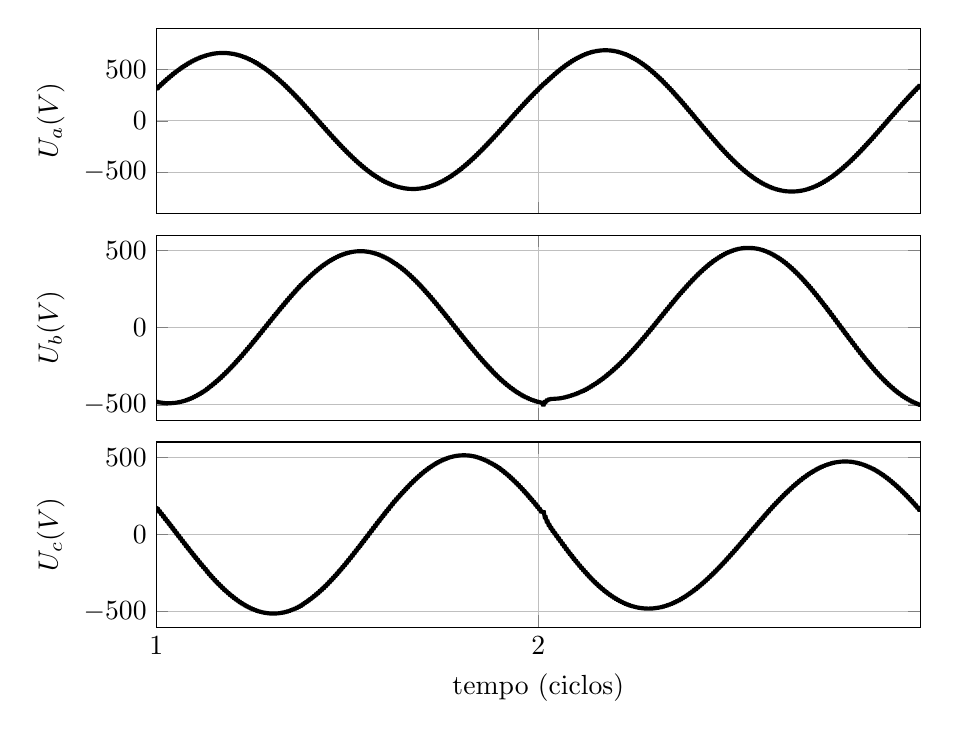
\begin{tikzpicture}

\begin{axis}[%
width=0.8\textwidth,
height=0.193917089240149\textwidth,
scale only axis,
xmin=0.0166666666666667,
xmax=0.05,
xtick={0,0.0166666666666667,0.0333333333333333},
xticklabels={\empty},
xmajorgrids,
ymin=-600,
ymax=600,
ytick={-500,    0,  500},
ylabel={$\text{U}_\text{b}\text{ (V)}$},
ymajorgrids,
name=plot2,
scaled x ticks = false,
legend columns=-1,
legend style={/tikz/every even column/.append style={column sep=0.3cm}},
legend style={font=\footnotesize}
]
\addplot [color=black,solid,line width=1.5pt,forget plot]
  table[row sep=crcr]{0.0166583333333333	-478.328989103039\\
0.0167	-481.372762295986\\
0.0167416666666667	-481.372762295986\\
0.0167833333333333	-483.944387417357\\
0.016825	-483.944387417357\\
0.0168666666666667	-486.043904769891\\
0.0169083333333333	-486.043904769891\\
0.01695	-487.669342075457\\
0.0169916666666667	-487.669342075457\\
0.0170333333333333	-488.81912329053\\
0.017075	-488.81912329053\\
0.0171166666666667	-489.492376222951\\
0.0171583333333333	-489.492376222951\\
0.0172	-489.689089295181\\
0.0172416666666667	-489.689089295181\\
0.0172833333333333	-489.410057478733\\
0.017325	-489.410057478733\\
0.0173666666666667	-488.656714544629\\
0.0174083333333333	-488.656714544629\\
0.01745	-487.430933830334\\
0.0174916666666667	-487.430933830334\\
0.0175333333333333	-485.734862735459\\
0.017575	-485.734862735459\\
0.0176166666666667	-483.570824107468\\
0.0176583333333333	-483.570824107468\\
0.0177	-480.941176730971\\
0.0177416666666667	-480.941176730971\\
0.0177833333333333	-477.848873406491\\
0.017825	-477.848873406491\\
0.0178666666666667	-474.296687037085\\
0.0179083333333333	-474.296687037085\\
0.01795	-470.287554266504\\
0.0179916666666667	-470.287554266504\\
0.0180333333333333	-465.824994538518\\
0.018075	-465.824994538518\\
0.0181166666666667	-460.912896166831\\
0.0181583333333333	-460.912896166831\\
0.0182	-455.555544349316\\
0.0182416666666667	-455.555544349316\\
0.0182833333333333	-449.757632700212\\
0.018325	-449.757632700212\\
0.0183666666666667	-443.524266807923\\
0.0184083333333333	-443.524266807923\\
0.01845	-436.860963041735\\
0.0184916666666667	-436.860963041735\\
0.0185333333333333	-429.773645406549\\
0.018575	-429.773645406549\\
0.0186166666666667	-422.2686421737\\
0.0186583333333333	-422.2686421737\\
0.0187	-414.352682994809\\
0.0187416666666667	-414.352682994809\\
0.0187833333333333	-406.710604021129\\
0.018825	-406.710604021129\\
0.0188666666666667	-396.968651829484\\
0.0189083333333333	-396.968651829484\\
0.01895	-387.24430030011\\
0.0189916666666667	-387.24430030011\\
0.0190333333333333	-377.413842111121\\
0.019075	-377.413842111121\\
0.0191166666666667	-367.3960735467\\
0.0191583333333333	-367.3960735467\\
0.0192	-357.12553953726\\
0.0192416666666667	-357.12553953726\\
0.0192833333333333	-346.559303382721\\
0.019325	-346.559303382721\\
0.0193666666666667	-335.674936708767\\
0.0194083333333333	-335.674936708767\\
0.01945	-324.465686057335\\
0.0194916666666667	-324.465686057335\\
0.0195333333333333	-312.935239244225\\
0.019575	-312.935239244225\\
0.0196166666666667	-301.093266862382\\
0.0196583333333333	-301.093266862382\\
0.0197	-288.95219973374\\
0.0197416666666667	-288.95219973374\\
0.0197833333333333	-276.525463982029\\
0.019825	-276.525463982029\\
0.0198666666666667	-263.82538033546\\
0.0199083333333333	-263.82538033546\\
0.01995	-250.865057706918\\
0.0199916666666667	-250.865057706918\\
0.0200333333333333	-237.656697428642\\
0.020075	-237.656697428642\\
0.0201166666666667	-224.212271375033\\
0.0201583333333333	-224.212271375033\\
0.0202	-210.543848998092\\
0.0202416666666667	-210.543848998092\\
0.0202833333333333	-196.6637735981\\
0.020325	-196.6637735981\\
0.0203666666666667	-182.584756063204\\
0.0204083333333333	-182.584756063204\\
0.02045	-168.319897946886\\
0.0204916666666667	-168.319897946886\\
0.0205333333333333	-153.882668002172\\
0.020575	-153.882668002172\\
0.0206166666666667	-139.286855686717\\
0.0206583333333333	-139.286855686717\\
0.0207	-124.546519243168\\
0.0207416666666667	-124.546519243168\\
0.0207833333333333	-109.675923407492\\
0.020825	-109.675923407492\\
0.0208666666666667	-94.6884951690301\\
0.0209083333333333	-94.6884951690301\\
0.02095	-79.6023211852309\\
0.0209916666666667	-79.6023211852309\\
0.0210333333333333	-64.4296541414652\\
0.021075	-64.4296541414652\\
0.0211166666666667	-49.1854677870168\\
0.0211583333333333	-49.1854677870168\\
0.0212	-33.8847697005379\\
0.0212416666666667	-33.8847697005379\\
0.0212833333333333	-18.5423320716325\\
0.021325	-18.5423320716325\\
0.0213666666666667	-3.1725945533516\\
0.0214083333333333	-3.1725945533516\\
0.02145	12.2102617721841\\
0.0214916666666667	12.2102617721841\\
0.0215333333333333	27.5921432856442\\
0.021575	27.5921432856442\\
0.0216166666666667	42.9588704890498\\
0.0216583333333333	42.9588704890498\\
0.0217	58.2960537853681\\
0.0217416666666667	58.2960537853681\\
0.0217833333333333	73.5890384864759\\
0.021825	73.5890384864759\\
0.0218666666666667	88.82269659409\\
0.0219083333333333	88.82269659409\\
0.02195	103.982669291038\\
0.0219916666666667	103.982669291038\\
0.0220333333333333	119.053037141893\\
0.022075	119.053037141893\\
0.0221166666666667	134.01853586672\\
0.0221583333333333	134.01853586672\\
0.0222	148.863909368128\\
0.0222416666666667	148.863909368128\\
0.0222833333333333	163.573956427556\\
0.022325	163.573956427556\\
0.0223666666666667	178.133568427636\\
0.0224083333333333	178.133568427636\\
0.02245	192.527757716713\\
0.0224916666666667	192.527757716713\\
0.0225333333333333	206.741679404245\\
0.022575	206.741679404245\\
0.0226166666666667	220.760649670751\\
0.0226583333333333	220.760649670751\\
0.0227	234.570162946369\\
0.0227416666666667	234.570162946369\\
0.0227833333333333	248.155909263895\\
0.022825	248.155909263895\\
0.0228666666666667	261.687830320942\\
0.0229083333333333	261.687830320942\\
0.02295	274.986604079196\\
0.0229916666666667	274.986604079196\\
0.0230333333333333	286.928801747272\\
0.023075	286.928801747272\\
0.0231166666666667	298.950506950644\\
0.0231583333333333	298.950506950644\\
0.0232	310.924864102034\\
0.0232416666666667	310.924864102034\\
0.0232833333333333	322.756989832147\\
0.023325	322.756989832147\\
0.0233666666666667	334.367084014297\\
0.0234083333333333	334.367084014297\\
0.02345	345.69602196514\\
0.0234916666666667	345.69602196514\\
0.0235333333333333	356.703461032175\\
0.023575	356.703461032175\\
0.0236166666666667	367.363371170442\\
0.0236583333333333	367.363371170442\\
0.0237	377.659204280424\\
0.0237416666666667	377.659204280424\\
0.0237833333333333	387.579795487262\\
0.023825	387.579795487262\\
0.0238666666666667	397.116425283701\\
0.0239083333333333	397.116425283701\\
0.02395	406.261310362139\\
0.0239916666666667	406.261310362139\\
0.0240333333333333	415.0053223807\\
0.024075	415.0053223807\\
0.0241166666666667	423.340732147141\\
0.0241583333333333	423.340732147141\\
0.0242	431.258683016742\\
0.0242416666666667	431.258683016742\\
0.0242833333333333	438.750365395371\\
0.024325	438.750365395371\\
0.0243666666666667	445.807262831054\\
0.0244083333333333	445.807262831054\\
0.02445	452.421342397773\\
0.0244916666666667	452.421342397773\\
0.0245333333333333	458.585161293933\\
0.024575	458.585161293933\\
0.0246166666666667	464.291905294308\\
0.0246583333333333	464.291905294308\\
0.0247	469.535383109734\\
0.0247416666666667	469.535383109734\\
0.0247833333333333	474.309999446141\\
0.024825	474.309999446141\\
0.0248666666666667	478.610723480444\\
0.0249083333333333	478.610723480444\\
0.02495	482.432523836755\\
0.0249916666666667	482.432523836755\\
0.0250333333333333	485.772612186125\\
0.025075	485.772612186125\\
0.0251166666666667	488.627883686145\\
0.0251583333333333	488.627883686145\\
0.0252	490.994391489966\\
0.0252416666666667	490.994391489966\\
0.0252833333333333	492.869784189106\\
0.025325	492.869784189106\\
0.0253666666666667	494.252063559781\\
0.0254083333333333	494.252063559781\\
0.02545	495.139387583695\\
0.0254916666666667	495.139387583695\\
0.0255333333333333	495.530061759552\\
0.025575	495.530061759552\\
0.0256166666666667	495.422663936061\\
0.0256583333333333	495.422663936061\\
0.0257	494.816230581684\\
0.0257416666666667	494.816230581684\\
0.0257833333333333	493.710425995119\\
0.025825	493.710425995119\\
0.0258666666666667	492.105654148384\\
0.0259083333333333	492.105654148384\\
0.02595	490.003108134894\\
0.0259916666666667	490.003108134894\\
0.0260333333333333	487.404961487327\\
0.026075	487.404961487327\\
0.0261166666666667	484.313069214194\\
0.0261583333333333	484.313069214194\\
0.0262	480.731558886196\\
0.0262416666666667	480.731558886196\\
0.0262833333333333	476.664323712434\\
0.026325	476.664323712434\\
0.0263666666666667	472.115829454631\\
0.0264083333333333	472.115829454631\\
0.02645	467.091068733291\\
0.0264916666666667	467.091068733291\\
0.0265333333333333	461.595540479995\\
0.026575	461.595540479995\\
0.0266166666666667	455.635234907076\\
0.0266583333333333	455.635234907076\\
0.0267	449.21662231492\\
0.0267416666666667	449.21662231492\\
0.0267833333333333	442.346643428456\\
0.026825	442.346643428456\\
0.0268666666666667	435.032699614098\\
0.0269083333333333	435.032699614098\\
0.02695	427.282642172915\\
0.0269916666666667	427.282642172915\\
0.0270333333333333	418.527982244731\\
0.027075	418.527982244731\\
0.0271166666666667	410.672570182659\\
0.0271583333333333	410.672570182659\\
0.0272	402.276872290978\\
0.0272416666666667	402.276872290978\\
0.0272833333333333	393.223850223727\\
0.027325	393.223850223727\\
0.0273666666666667	383.609151155178\\
0.0274083333333333	383.609151155178\\
0.02745	373.508718653929\\
0.0274916666666667	373.508718653929\\
0.0275333333333333	362.979579538073\\
0.027575	362.979579538073\\
0.0276166666666667	352.061894709897\\
0.0276583333333333	352.061894709897\\
0.0277	340.783205444461\\
0.0277416666666667	340.783205444461\\
0.0277833333333333	329.162781541968\\
0.027825	329.162781541968\\
0.0278666666666667	317.215226351439\\
0.0279083333333333	317.215226351439\\
0.02795	304.953068995059\\
0.0279916666666667	304.953068995059\\
0.0280333333333333	292.388308765939\\
0.028075	292.388308765939\\
0.0281166666666667	279.533394256386\\
0.0281583333333333	279.533394256386\\
0.0282	266.401997020689\\
0.0282416666666667	266.401997020689\\
0.0282833333333333	253.007121767018\\
0.028325	253.007121767018\\
0.0283666666666667	239.363037342399\\
0.0284083333333333	239.363037342399\\
0.02845	225.484309796947\\
0.0284916666666667	225.484309796947\\
0.0285333333333333	211.385672071801\\
0.028575	211.385672071801\\
0.0286166666666667	197.081935254737\\
0.0286583333333333	197.081935254737\\
0.0287	182.587950486431\\
0.0287416666666667	182.587950486431\\
0.0287833333333333	167.918604082923\\
0.028825	167.918604082923\\
0.0288666666666667	153.088829011011\\
0.0289083333333333	153.088829011011\\
0.02895	138.113619934855\\
0.0289916666666667	138.113619934855\\
0.0290333333333333	123.008044204917\\
0.029075	123.008044204917\\
0.0291166666666667	107.788100944899\\
0.0291583333333333	107.788100944899\\
0.0292	92.4664220892656\\
0.0292416666666667	92.4664220892656\\
0.0292833333333333	77.0599110293703\\
0.029325	77.0599110293703\\
0.0293666666666667	61.5839402726698\\
0.0294083333333333	61.5839402726698\\
0.02945	46.0538191073489\\
0.0294916666666667	46.0538191073489\\
0.0295333333333333	30.4851141949034\\
0.029575	30.4851141949034\\
0.0296166666666667	14.8937682112207\\
0.0296583333333333	14.8937682112207\\
0.0297	-0.703957306529608\\
0.0297416666666667	-0.703957306529608\\
0.0297833333333333	-16.2916492298269\\
0.029825	-16.2916492298269\\
0.0298666666666667	-31.8529362123827\\
0.0299083333333333	-31.8529362123827\\
0.02995	-47.371649369948\\
0.0299916666666667	-47.371649369948\\
0.0300333333333333	-62.8319222299047\\
0.030075	-62.8319222299047\\
0.0301166666666667	-78.2183969102601\\
0.0301583333333333	-78.2183969102601\\
0.0302	-93.5154108314719\\
0.0302416666666667	-93.5154108314719\\
0.0302833333333333	-108.70816278091\\
0.030325	-108.70816278091\\
0.0303666666666667	-123.782356080195\\
0.0304083333333333	-123.782356080195\\
0.03045	-138.723507249364\\
0.0304916666666667	-138.723507249364\\
0.0305333333333333	-153.517339096442\\
0.030575	-153.517339096442\\
0.0306166666666667	-168.149764544084\\
0.0306583333333333	-168.149764544084\\
0.0307	-182.60688669631\\
0.0307416666666667	-182.60688669631\\
0.0307833333333333	-196.875004412733\\
0.030825	-196.875004412733\\
0.0308666666666667	-210.940621254231\\
0.0309083333333333	-210.940621254231\\
0.03095	-224.790455634942\\
0.0309916666666667	-224.790455634942\\
0.0310333333333333	-238.411450801645\\
0.031075	-238.411450801645\\
0.0311166666666667	-251.788204920739\\
0.0311583333333333	-251.788204920739\\
0.0312	-264.319493294975\\
0.0312416666666667	-264.319493294975\\
0.0312833333333333	-278.081845363642\\
0.031325	-278.081845363642\\
0.0313666666666667	-291.211888263673\\
0.0314083333333333	-291.211888263673\\
0.03145	-303.807007713181\\
0.0314916666666667	-303.807007713181\\
0.0315333333333333	-315.936364357588\\
0.031575	-315.936364357588\\
0.0316166666666667	-327.655020751537\\
0.0316583333333333	-327.655020751537\\
0.0317	-338.998550237152\\
0.0317416666666667	-338.998550237152\\
0.0317833333333333	-349.984949605885\\
0.031825	-349.984949605885\\
0.0318666666666667	-360.618974262017\\
0.0319083333333333	-360.618974262017\\
0.03195	-370.896795074955\\
0.0319916666666667	-370.896795074955\\
0.0320333333333333	-380.809923421548\\
0.032075	-380.809923421548\\
0.0321166666666667	-390.348041070204\\
0.0321583333333333	-390.348041070204\\
0.0322	-399.500455565927\\
0.0322416666666667	-399.500455565927\\
0.0322833333333333	-408.258433783543\\
0.032325	-408.258433783543\\
0.0323666666666667	-416.612673979994\\
0.0324083333333333	-416.612673979994\\
0.03245	-424.555376388038\\
0.0324916666666667	-424.555376388038\\
0.0325333333333333	-432.079651399668\\
0.032575	-432.079651399668\\
0.0326166666666667	-439.17912856472\\
0.0326583333333333	-439.17912856472\\
0.0327	-445.847803165625\\
0.0327416666666667	-445.847803165625\\
0.0327833333333333	-452.079952433882\\
0.032825	-452.079952433882\\
0.0328666666666667	-457.870112681898\\
0.0329083333333333	-457.870112681898\\
0.03295	-463.213095942823\\
0.0329916666666667	-463.213095942823\\
0.0330333333333333	-468.104025539882\\
0.033075	-468.104025539882\\
0.0331166666666667	-472.538375275198\\
0.0331583333333333	-472.538375275198\\
0.0332	-476.512043591712\\
0.0332416666666667	-476.512043591712\\
0.0332833333333333	-480.021998518076\\
0.033325	-480.021998518076\\
0.0333666666666667	-483.062409528906\\
0.0334083333333333	-483.062409528906\\
0.03345	-485.632179354782\\
0.0334916666666667	-485.632179354782\\
0.0335333333333333	-498.998270566993\\
0.033575	-498.998270566993\\
0.0336166666666667	-481.782582963858\\
0.0336583333333333	-481.782582963858\\
0.0337	-471.288948850027\\
0.0337416666666667	-471.288948850027\\
0.0337833333333333	-465.459114040876\\
0.033825	-465.459114040876\\
0.0338666666666667	-462.647848629665\\
0.0339083333333333	-462.647848629665\\
0.03395	-461.417560400509\\
0.0339916666666667	-461.417560400509\\
0.0340333333333333	-460.731633382674\\
0.034075	-460.731633382674\\
0.0341166666666667	-459.951982625119\\
0.0341583333333333	-459.951982625119\\
0.0342	-458.758531093\\
0.0342416666666667	-458.758531093\\
0.0342833333333333	-457.045782912744\\
0.034325	-457.045782912744\\
0.0343666666666667	-454.82926213895\\
0.0344083333333333	-454.82926213895\\
0.03445	-452.172796925181\\
0.0344916666666667	-452.172796925181\\
0.0345333333333333	-449.145658792875\\
0.034575	-449.145658792875\\
0.0346166666666667	-445.800265404507\\
0.0346583333333333	-445.800265404507\\
0.0347	-442.166059354816\\
0.0347416666666667	-442.166059354816\\
0.0347833333333333	-438.252372103144\\
0.034825	-438.252372103144\\
0.0348666666666667	-434.054953798003\\
0.0349083333333333	-434.054953798003\\
0.03495	-429.562674435509\\
0.0349916666666667	-429.562674435509\\
0.0350333333333333	-424.762700040261\\
0.035075	-424.762700040261\\
0.0351166666666667	-419.643661421394\\
0.0351583333333333	-419.643661421394\\
0.0352	-414.197053720857\\
0.0352416666666667	-414.197053720857\\
0.0352833333333333	-408.523882649902\\
0.035325	-408.523882649902\\
0.0353666666666667	-402.479291356868\\
0.0354083333333333	-402.479291356868\\
0.03545	-395.601828599323\\
0.0354916666666667	-395.601828599323\\
0.0355333333333333	-388.546283162184\\
0.035575	-388.546283162184\\
0.0356166666666667	-381.262052118517\\
0.0356583333333333	-381.262052118517\\
0.0357	-373.714229076942\\
0.0357416666666667	-373.714229076942\\
0.0357833333333333	-365.874593646954\\
0.035825	-365.874593646954\\
0.0358666666666667	-357.724034021534\\
0.0359083333333333	-357.724034021534\\
0.03595	-349.251553064004\\
0.0359916666666667	-349.251553064004\\
0.0360333333333333	-340.452622235918\\
0.036075	-340.452622235918\\
0.0361166666666667	-331.327227991727\\
0.0361583333333333	-331.327227991727\\
0.0362	-321.878129980668\\
0.0362416666666667	-321.878129980668\\
0.0362833333333333	-312.109568466451\\
0.036325	-312.109568466451\\
0.0363666666666667	-302.026644843582\\
0.0364083333333333	-302.026644843582\\
0.03645	-291.63387748511\\
0.0364916666666667	-291.63387748511\\
0.0365333333333333	-280.937199605059\\
0.036575	-280.937199605059\\
0.0366166666666667	-269.942114366078\\
0.0366583333333333	-269.942114366078\\
0.0367	-258.654477866822\\
0.0367416666666667	-258.654477866822\\
0.0367833333333333	-247.080567388712\\
0.036825	-247.080567388712\\
0.0368666666666667	-235.227176729096\\
0.0369083333333333	-235.227176729096\\
0.03695	-223.101681785848\\
0.0369916666666667	-223.101681785848\\
0.0370333333333333	-210.712058862678\\
0.037075	-210.712058862678\\
0.0371166666666667	-198.066879573849\\
0.0371583333333333	-198.066879573849\\
0.0372	-185.175292454286\\
0.0372416666666667	-185.175292454286\\
0.0372833333333333	-172.046999319569\\
0.037325	-172.046999319569\\
0.0373666666666667	-158.692016960269\\
0.0374083333333333	-158.692016960269\\
0.03745	-145.121500911102\\
0.0374916666666667	-145.121500911102\\
0.0375333333333333	-131.346961858294\\
0.037575	-131.346961858294\\
0.0376166666666667	-117.380802663719\\
0.0376583333333333	-117.380802663719\\
0.0377	-103.235234173154\\
0.0377416666666667	-103.235234173154\\
0.0377833333333333	-88.9164304808335\\
0.037825	-88.9164304808335\\
0.0378666666666667	-74.439342100256\\
0.0379083333333333	-74.439342100256\\
0.03795	-59.8184609425996\\
0.0379916666666667	-59.8184609425996\\
0.0380333333333333	-45.0680374599692\\
0.038075	-45.0680374599692\\
0.0381166666666667	-30.2022370755135\\
0.0381583333333333	-30.2022370755135\\
0.0382	-15.2353217495658\\
0.0382416666666667	-15.2353217495658\\
0.0382833333333333	-0.181794007753641\\
0.038325	-0.181794007753641\\
0.0383666666666667	14.9435042350192\\
0.0384083333333333	14.9435042350192\\
0.03845	30.1252956286667\\
0.0384916666666667	30.1252956286667\\
0.0385333333333333	45.3486629556394\\
0.038575	45.3486629556394\\
0.0386166666666667	60.5972401707852\\
0.0386583333333333	60.5972401707852\\
0.0387	75.8549297738552\\
0.0387416666666667	75.8549297738552\\
0.0387833333333333	91.1054325668948\\
0.038825	91.1054325668948\\
0.0388666666666667	106.332243601449\\
0.0389083333333333	106.332243601449\\
0.03895	121.518722394686\\
0.0389916666666667	121.518722394686\\
0.0390333333333333	136.648130986171\\
0.039075	136.648130986171\\
0.0391166666666667	151.703658745296\\
0.0391583333333333	151.703658745296\\
0.0392	166.6684438936\\
0.0392416666666667	166.6684438936\\
0.0392833333333333	181.525594900189\\
0.039325	181.525594900189\\
0.0393666666666667	196.258213496354\\
0.0394083333333333	196.258213496354\\
0.03945	211.11916789107\\
0.0394916666666667	211.11916789107\\
0.0395333333333333	225.228256753655\\
0.039575	225.228256753655\\
0.0396166666666667	239.176704133903\\
0.0396583333333333	239.176704133903\\
0.0397	253.050541633453\\
0.0397416666666667	253.050541633453\\
0.0397833333333333	266.794622440343\\
0.039825	266.794622440343\\
0.0398666666666667	280.36352639823\\
0.0399083333333333	280.36352639823\\
0.03995	293.720079804169\\
0.0399916666666667	293.720079804169\\
0.0400333333333333	306.834840978919\\
0.040075	306.834840978919\\
0.0401166666666667	319.684432072053\\
0.0401583333333333	319.684432072053\\
0.0402	332.249529221863\\
0.0402416666666667	332.249529221863\\
0.0402833333333333	344.513518148991\\
0.040325	344.513518148991\\
0.0403666666666667	356.461398472636\\
0.0404083333333333	356.461398472636\\
0.04045	368.07906117244\\
0.0404916666666667	368.07906117244\\
0.0405333333333333	379.352665704272\\
0.040575	379.352665704272\\
0.0406166666666667	390.268254951875\\
0.0406583333333333	390.268254951875\\
0.0407	400.81284512302\\
0.0407416666666667	400.81284512302\\
0.0407833333333333	410.973175722926\\
0.040825	410.973175722926\\
0.0408666666666667	420.736369760103\\
0.0409083333333333	420.736369760103\\
0.04095	430.089939730837\\
0.0409916666666667	430.089939730837\\
0.0410333333333333	439.02189748336\\
0.041075	439.02189748336\\
0.0411166666666667	447.520797951081\\
0.0411583333333333	447.520797951081\\
0.0412	455.57576068455\\
0.0412416666666667	455.57576068455\\
0.0412833333333333	463.176477754051\\
0.041325	463.176477754051\\
0.0413666666666667	470.313215198367\\
0.0414083333333333	470.313215198367\\
0.04145	476.976813020432\\
0.0414916666666667	476.976813020432\\
0.0415333333333333	483.158335808922\\
0.041575	483.158335808922\\
0.0416166666666667	488.850790106914\\
0.0416583333333333	488.850790106914\\
0.0417	494.046217480564\\
0.0417416666666667	494.046217480564\\
0.0417833333333333	498.740107259914\\
0.041825	498.740107259914\\
0.0418666666666667	502.92186011784\\
0.0419083333333333	502.92186011784\\
0.04195	506.583545623777\\
0.0419916666666667	506.583545623777\\
0.0420333333333333	509.721710214485\\
0.042075	509.721710214485\\
0.0421166666666667	512.332784100593\\
0.0421583333333333	512.332784100593\\
0.0422	514.413279158182\\
0.0422416666666667	514.413279158182\\
0.0422833333333333	515.9599757688\\
0.042325	515.9599757688\\
0.0423666666666667	516.970100515159\\
0.0424083333333333	516.970100515159\\
0.04245	517.441480758459\\
0.0424916666666667	517.441480758459\\
0.0425333333333333	517.372752150282\\
0.042575	517.372752150282\\
0.0426166666666667	516.762847399441\\
0.0426583333333333	516.762847399441\\
0.0427	515.611781315798\\
0.0427416666666667	515.611781315798\\
0.0427833333333333	513.92048533442\\
0.042825	513.92048533442\\
0.0428666666666667	511.690288385606\\
0.0429083333333333	511.690288385606\\
0.04295	508.923157960981\\
0.0429916666666667	508.923157960981\\
0.0430333333333333	505.62173995849\\
0.043075	505.62173995849\\
0.0431166666666667	501.78931073118\\
0.0431583333333333	501.78931073118\\
0.0432	497.429767725351\\
0.0432416666666667	497.429767725351\\
0.0432833333333333	492.547621632959\\
0.043325	492.547621632959\\
0.0433666666666667	487.14798908254\\
0.0434083333333333	487.14798908254\\
0.04345	481.236584761708\\
0.0434916666666667	481.236584761708\\
0.0435333333333333	474.813193437904\\
0.043575	474.813193437904\\
0.0436166666666667	467.617975016633\\
0.0436583333333333	467.617975016633\\
0.0437	460.640009785613\\
0.0437416666666667	460.640009785613\\
0.0437833333333333	453.026742559859\\
0.043825	453.026742559859\\
0.0438666666666667	444.829079350061\\
0.0439083333333333	444.829079350061\\
0.04395	436.091902638318\\
0.0439916666666667	436.091902638318\\
0.0440333333333333	426.854279959608\\
0.044075	426.854279959608\\
0.0441166666666667	417.147056125927\\
0.0441583333333333	417.147056125927\\
0.0442	406.993617805562\\
0.0442416666666667	406.993617805562\\
0.0442833333333333	396.411764190075\\
0.044325	396.411764190075\\
0.0443666666666667	385.415729474773\\
0.0444083333333333	385.415729474773\\
0.04445	374.017909476246\\
0.0444916666666667	374.017909476246\\
0.0445333333333333	362.230108715941\\
0.044575	362.230108715941\\
0.0446166666666667	350.064119512135\\
0.0446583333333333	350.064119512135\\
0.0447	337.533091230516\\
0.0447416666666667	337.533091230516\\
0.0447833333333333	324.649922144971\\
0.044825	324.649922144971\\
0.0448666666666667	311.428439890778\\
0.0449083333333333	311.428439890778\\
0.04495	297.883125554185\\
0.0449916666666667	297.883125554185\\
0.0450333333333333	284.028841924275\\
0.045075	284.028841924275\\
0.0451166666666667	269.880782608134\\
0.0451583333333333	269.880782608134\\
0.0452	255.454385329104\\
0.0452416666666667	255.454385329104\\
0.0452833333333333	240.765301798375\\
0.045325	240.765301798375\\
0.0453666666666667	225.829384538562\\
0.0454083333333333	225.829384538562\\
0.04545	210.662681339409\\
0.0454916666666667	210.662681339409\\
0.0455333333333333	195.281430438134\\
0.045575	195.281430438134\\
0.0456166666666667	179.702077212704\\
0.0456583333333333	179.702077212704\\
0.0457	163.941485539902\\
0.0457416666666667	163.941485539902\\
0.0457833333333333	148.015394086019\\
0.045825	148.015394086019\\
0.0458666666666667	131.941232581943\\
0.0459083333333333	131.941232581943\\
0.04595	115.733018226992\\
0.0459916666666667	115.733018226992\\
0.0460333333333333	99.4155506737076\\
0.046075	99.4155506737076\\
0.0461166666666667	83.0048753817104\\
0.0461583333333333	83.0048753817104\\
0.0462	66.5169842374124\\
0.0462416666666667	66.5169842374124\\
0.0462833333333333	49.9685533749797\\
0.046325	49.9685533749797\\
0.0463666666666667	33.3767580588298\\
0.0464083333333333	33.3767580588298\\
0.04645	16.7590504552267\\
0.0464916666666667	16.7590504552267\\
0.0465333333333333	0.132970181758703\\
0.046575	0.132970181758703\\
0.0466166666666667	-16.4839901619608\\
0.0466583333333333	-16.4839901619608\\
0.0467	-33.0746636693815\\
0.0467416666666667	-33.0746636693815\\
0.0467833333333333	-49.6211722773108\\
0.046825	-49.6211722773108\\
0.0468666666666667	-66.1070457181566\\
0.0469083333333333	-66.1070457181566\\
0.04695	-82.5154452365718\\
0.0469916666666667	-82.5154452365718\\
0.0470333333333333	-98.8296440709486\\
0.047075	-98.8296440709486\\
0.0471166666666667	-115.033091242092\\
0.0471583333333333	-115.033091242092\\
0.0472	-131.109433370824\\
0.0472416666666667	-131.109433370824\\
0.0472833333333333	-147.042503492819\\
0.047325	-147.042503492819\\
0.0473666666666667	-162.816333505291\\
0.0474083333333333	-162.816333505291\\
0.04745	-178.41516835848\\
0.0474916666666667	-178.41516835848\\
0.0475333333333333	-193.8234809494\\
0.047575	-193.8234809494\\
0.0476166666666667	-209.025986747927\\
0.0476583333333333	-209.025986747927\\
0.0477	-223.904186047126\\
0.0477416666666667	-223.904186047126\\
0.0477833333333333	-238.606857549563\\
0.047825	-238.606857549563\\
0.0478666666666667	-253.47478702492\\
0.0479083333333333	-253.47478702492\\
0.04795	-267.938417779568\\
0.0479916666666667	-267.938417779568\\
0.0480333333333333	-282.029617204579\\
0.048075	-282.029617204579\\
0.0481166666666667	-295.766635150869\\
0.0481583333333333	-295.766635150869\\
0.0482	-309.161799602257\\
0.0482416666666667	-309.161799602257\\
0.0482833333333333	-322.219833483858\\
0.048325	-322.219833483858\\
0.0483666666666667	-334.938825256652\\
0.0484083333333333	-334.938825256652\\
0.04845	-347.312016422018\\
0.0484916666666667	-347.312016422018\\
0.0485333333333333	-359.329644222863\\
0.048575	-359.329644222863\\
0.0486166666666667	-370.980465786804\\
0.0486583333333333	-370.980465786804\\
0.0487	-382.252844743103\\
0.0487416666666667	-382.252844743103\\
0.0487833333333333	-393.135216849012\\
0.048825	-393.135216849012\\
0.0488666666666667	-403.617584174739\\
0.0489083333333333	-403.617584174739\\
0.04895	-413.689218945276\\
0.0489916666666667	-413.689218945276\\
0.0490333333333333	-423.340771462502\\
0.049075	-423.340771462502\\
0.0491166666666667	-432.563452770036\\
0.0491583333333333	-432.563452770036\\
0.0492	-441.348991482752\\
0.0492416666666667	-441.348991482752\\
0.0492833333333333	-449.689568336581\\
0.049325	-449.689568336581\\
0.0493666666666667	-457.577772446396\\
0.0494083333333333	-457.577772446396\\
0.04945	-465.006594338065\\
0.0494916666666667	-465.006594338065\\
0.0495333333333333	-471.969434299032\\
0.049575	-471.969434299032\\
0.0496166666666667	-478.460118028508\\
0.0496583333333333	-478.460118028508\\
0.0497	-484.472913508959\\
0.0497416666666667	-484.472913508959\\
0.0497833333333333	-490.002697136551\\
0.049825	-490.002697136551\\
0.0498666666666667	-495.044403692677\\
0.0499083333333333	-495.044403692677\\
0.04995	-499.593400120443\\
0.0499916666666667	-499.593400120443\\
};
\end{axis}

\begin{axis}[%
width=0.8\textwidth,
height=0.193917089240149\textwidth,
scale only axis,
xmin=0.0166666666666667,
xmax=0.05,
xtick={0,0.0166666666666667,0.0333333333333333},
xticklabels={{0},{1},{2}},
xlabel={tempo (ciclos)},
xmajorgrids,
ymin=-600,
ymax=600,
ytick={-500,    0,  500},
ylabel={$\text{U}_\text{c}\text{ (V)}$},
ymajorgrids,
at=(plot2.below south west),
anchor=above north west,
scaled x ticks = false,
legend columns=-1,
legend style={/tikz/every even column/.append style={column sep=0.3cm}},
legend style={font=\footnotesize}
]
\addplot [color=black,solid,line width=1.5pt,forget plot]
  table[row sep=crcr]{0.0166583333333333	180.146044285981\\
0.0167	164.940320934484\\
0.0167416666666667	164.940320934484\\
0.0167833333333333	149.579587477261\\
0.016825	149.579587477261\\
0.0168666666666667	134.079551509137\\
0.0169083333333333	134.079551509137\\
0.01695	118.455249604828\\
0.0169916666666667	118.455249604828\\
0.0170333333333333	102.721820759597\\
0.017075	102.721820759597\\
0.0171166666666667	86.8947024886041\\
0.0171583333333333	86.8947024886041\\
0.0172	70.9897152347551\\
0.0172416666666667	70.9897152347551\\
0.0172833333333333	55.0229884605968\\
0.017325	55.0229884605968\\
0.0173666666666667	39.0107951391398\\
0.0174083333333333	39.0107951391398\\
0.01745	22.9693692316446\\
0.0174916666666667	22.9693692316446\\
0.0175333333333333	6.91476165823279\\
0.017575	6.91476165823279\\
0.0176166666666667	-9.13724020053355\\
0.0176583333333333	-9.13724020053355\\
0.0177	-25.1712876244939\\
0.0177416666666667	-25.1712876244939\\
0.0177833333333333	-41.1717016099994\\
0.017825	-41.1717016099994\\
0.0178666666666667	-57.1235450619316\\
0.0179083333333333	-57.1235450619316\\
0.01795	-73.0122416753861\\
0.0179916666666667	-73.0122416753861\\
0.0180333333333333	-88.8229904086394\\
0.018075	-88.8229904086394\\
0.0181166666666667	-104.541092542183\\
0.0181583333333333	-104.541092542183\\
0.0182	-120.151937938219\\
0.0182416666666667	-120.151937938219\\
0.0182833333333333	-135.641005542097\\
0.018325	-135.641005542097\\
0.0183666666666667	-150.993870043721\\
0.0184083333333333	-150.993870043721\\
0.01845	-166.196212093992\\
0.0184916666666667	-166.196212093992\\
0.0185333333333333	-181.2338298443\\
0.018575	-181.2338298443\\
0.0186166666666667	-196.092650491087\\
0.0186583333333333	-196.092650491087\\
0.0187	-210.758741337919\\
0.0187416666666667	-210.758741337919\\
0.0187833333333333	-224.272823986116\\
0.018825	-224.272823986116\\
0.0188666666666667	-239.924185188171\\
0.0189083333333333	-239.924185188171\\
0.01895	-254.795099361687\\
0.0189916666666667	-254.795099361687\\
0.0190333333333333	-269.036557729883\\
0.019075	-269.036557729883\\
0.0191166666666667	-282.760389233867\\
0.0191583333333333	-282.760389233867\\
0.0192	-296.057851197266\\
0.0192416666666667	-296.057851197266\\
0.0192833333333333	-308.990098283122\\
0.019325	-308.990098283122\\
0.0193666666666667	-321.590393418407\\
0.0194083333333333	-321.590393418407\\
0.01945	-333.870571911174\\
0.0194916666666667	-333.870571911174\\
0.0195333333333333	-345.828322444006\\
0.019575	-345.828322444006\\
0.0196166666666667	-357.453508661192\\
0.0196583333333333	-357.453508661192\\
0.0197	-368.732790011102\\
0.0197416666666667	-368.732790011102\\
0.0197833333333333	-379.652185798579\\
0.019825	-379.652185798579\\
0.0198666666666667	-390.200039679523\\
0.0199083333333333	-390.200039679523\\
0.01995	-400.364455853375\\
0.0199916666666667	-400.364455853375\\
0.0200333333333333	-410.135593074462\\
0.020075	-410.135593074462\\
0.0201166666666667	-419.504723697965\\
0.0201583333333333	-419.504723697965\\
0.0202	-428.463752199279\\
0.0202416666666667	-428.463752199279\\
0.0202833333333333	-437.004944992871\\
0.020325	-437.004944992871\\
0.0203666666666667	-445.120779808899\\
0.0204083333333333	-445.120779808899\\
0.02045	-452.8038978512\\
0.0204916666666667	-452.8038978512\\
0.0205333333333333	-460.047124180064\\
0.020575	-460.047124180064\\
0.0206166666666667	-466.843522119401\\
0.0206583333333333	-466.843522119401\\
0.0207	-473.186455823302\\
0.0207416666666667	-473.186455823302\\
0.0207833333333333	-479.069643185327\\
0.020825	-479.069643185327\\
0.0208666666666667	-484.487584080736\\
0.0209083333333333	-484.487584080736\\
0.02095	-489.433644253288\\
0.0209916666666667	-489.433644253288\\
0.0210333333333333	-493.903539136153\\
0.021075	-493.903539136153\\
0.0211166666666667	-497.892633124744\\
0.0211583333333333	-497.892633124744\\
0.0212	-501.396820907034\\
0.0212416666666667	-501.396820907034\\
0.0212833333333333	-504.41270742765\\
0.021325	-504.41270742765\\
0.0213666666666667	-506.937652408911\\
0.0214083333333333	-506.937652408911\\
0.02145	-508.969679717527\\
0.0214916666666667	-508.969679717527\\
0.0215333333333333	-510.507315547184\\
0.021575	-510.507315547184\\
0.0216166666666667	-511.549437470117\\
0.0216583333333333	-511.549437470117\\
0.0217	-512.095173916005\\
0.0217416666666667	-512.095173916005\\
0.0217833333333333	-512.14386626104\\
0.021825	-512.14386626104\\
0.0218666666666667	-511.694775425209\\
0.0219083333333333	-511.694775425209\\
0.02195	-510.748811874119\\
0.0219916666666667	-510.748811874119\\
0.0220333333333333	-509.305240015087\\
0.022075	-509.305240015087\\
0.0221166666666667	-507.364690126307\\
0.0221583333333333	-507.364690126307\\
0.0222	-504.928245184668\\
0.0222416666666667	-504.928245184668\\
0.0222833333333333	-501.997459837756\\
0.022325	-501.997459837756\\
0.0223666666666667	-498.57437873634\\
0.0224083333333333	-498.57437873634\\
0.02245	-494.661546862205\\
0.0224916666666667	-494.661546862205\\
0.0225333333333333	-490.262014038761\\
0.022575	-490.262014038761\\
0.0226166666666667	-485.379336077746\\
0.0226583333333333	-485.379336077746\\
0.0227	-480.017574398345\\
0.0227416666666667	-480.017574398345\\
0.0227833333333333	-474.181295093699\\
0.022825	-474.181295093699\\
0.0228666666666667	-468.132227564933\\
0.0229083333333333	-468.132227564933\\
0.02295	-461.649789032895\\
0.0229916666666667	-461.649789032895\\
0.0230333333333333	-453.193902270209\\
0.023075	-453.193902270209\\
0.0231166666666667	-444.773441113673\\
0.0231583333333333	-444.773441113673\\
0.0232	-436.251268459993\\
0.0232416666666667	-436.251268459993\\
0.0232833333333333	-427.520263672964\\
0.023325	-427.520263672964\\
0.0233666666666667	-418.493740302993\\
0.0234083333333333	-418.493740302993\\
0.02345	-409.11363513705\\
0.0234916666666667	-409.11363513705\\
0.0235333333333333	-399.348350327473\\
0.023575	-399.348350327473\\
0.0236166666666667	-389.186670490501\\
0.0236583333333333	-389.186670490501\\
0.0237	-378.630905372963\\
0.0237416666666667	-378.630905372963\\
0.0237833333333333	-367.690968950489\\
0.023825	-367.690968950489\\
0.0238666666666667	-356.380102358096\\
0.0239083333333333	-356.380102358096\\
0.02395	-344.712640572405\\
0.0239916666666667	-344.712640572405\\
0.0240333333333333	-332.700781505562\\
0.024075	-332.700781505562\\
0.0241166666666667	-320.358317577706\\
0.0241583333333333	-320.358317577706\\
0.0242	-307.6971824162\\
0.0242416666666667	-307.6971824162\\
0.0242833333333333	-294.729044137296\\
0.024325	-294.729044137296\\
0.0243666666666667	-281.465654636295\\
0.0244083333333333	-281.465654636295\\
0.02445	-267.919108296558\\
0.0244916666666667	-267.919108296558\\
0.0245333333333333	-254.101977634579\\
0.024575	-254.101977634579\\
0.0246166666666667	-240.027348361342\\
0.0246583333333333	-240.027348361342\\
0.0247	-225.708789227798\\
0.0247416666666667	-225.708789227798\\
0.0247833333333333	-211.160290317149\\
0.024825	-211.160290317149\\
0.0248666666666667	-196.39619457631\\
0.0249083333333333	-196.39619457631\\
0.02495	-181.431040895376\\
0.0249916666666667	-181.431040895376\\
0.0250333333333333	-166.279778355741\\
0.025075	-166.279778355741\\
0.0251166666666667	-150.957981557132\\
0.0251583333333333	-150.957981557132\\
0.0252	-135.480589084291\\
0.0252416666666667	-135.480589084291\\
0.0252833333333333	-119.863094908503\\
0.025325	-119.863094908503\\
0.0253666666666667	-104.121014925928\\
0.0254083333333333	-104.121014925928\\
0.02545	-88.2697324252375\\
0.0254916666666667	-88.2697324252375\\
0.0255333333333333	-72.3244975934466\\
0.025575	-72.3244975934466\\
0.0256166666666667	-56.3005347394663\\
0.0256583333333333	-56.3005347394663\\
0.0257	-40.2131789209932\\
0.0257416666666667	-40.2131789209932\\
0.0257833333333333	-24.0779930748701\\
0.025825	-24.0779930748701\\
0.0258666666666667	-7.91083206935371\\
0.0259083333333333	-7.91083206935371\\
0.02595	8.27214526930201\\
0.0259916666666667	8.27214526930201\\
0.0260333333333333	24.4542254440382\\
0.026075	24.4542254440382\\
0.0261166666666667	40.6199908695603\\
0.0261583333333333	40.6199908695603\\
0.0262	56.7516612117422\\
0.0262416666666667	56.7516612117422\\
0.0262833333333333	72.8325712785133\\
0.026325	72.8325712785133\\
0.0263666666666667	88.846063325594\\
0.0264083333333333	88.846063325594\\
0.02645	104.775539088676\\
0.0264916666666667	104.775539088676\\
0.0265333333333333	120.604489043941\\
0.026575	120.604489043941\\
0.0266166666666667	136.316517603678\\
0.0266583333333333	136.316517603678\\
0.0267	151.895365005857\\
0.0267416666666667	151.895365005857\\
0.0267833333333333	167.32492740609\\
0.026825	167.32492740609\\
0.0268666666666667	182.589276240632\\
0.0269083333333333	182.589276240632\\
0.02695	197.67267733356\\
0.0269916666666667	197.67267733356\\
0.0270333333333333	213.364075445209\\
0.027075	213.364075445209\\
0.0271166666666667	227.019890089968\\
0.0271583333333333	227.019890089968\\
0.0272	240.616905132375\\
0.0272416666666667	240.616905132375\\
0.0272833333333333	254.329291302055\\
0.027325	254.329291302055\\
0.0273666666666667	268.025476997475\\
0.0274083333333333	268.025476997475\\
0.02745	281.599414976171\\
0.0274916666666667	281.599414976171\\
0.0275333333333333	294.97178527555\\
0.027575	294.97178527555\\
0.0276166666666667	308.087625765951\\
0.0276583333333333	308.087625765951\\
0.0277	320.910690989392\\
0.0277416666666667	320.910690989392\\
0.0277833333333333	333.417415766459\\
0.027825	333.417415766459\\
0.0278666666666667	345.591780478394\\
0.0279083333333333	345.591780478394\\
0.02795	357.421558389868\\
0.0279916666666667	357.421558389868\\
0.0280333333333333	368.896047770843\\
0.028075	368.896047770843\\
0.0281166666666667	380.004638133566\\
0.0281583333333333	380.004638133566\\
0.0282	390.735700889524\\
0.0282416666666667	390.735700889524\\
0.0282833333333333	401.079183264076\\
0.028325	401.079183264076\\
0.0283666666666667	411.023979838759\\
0.0284083333333333	411.023979838759\\
0.02845	420.559255161147\\
0.0284916666666667	420.559255161147\\
0.0285333333333333	429.674638195389\\
0.028575	429.674638195389\\
0.0286166666666667	438.36034696872\\
0.0286583333333333	438.36034696872\\
0.0287	446.607237052018\\
0.0287416666666667	446.607237052018\\
0.0287833333333333	454.406798841608\\
0.028825	454.406798841608\\
0.0288666666666667	461.751128592088\\
0.0289083333333333	461.751128592088\\
0.02895	468.632892411405\\
0.0289916666666667	468.632892411405\\
0.0290333333333333	475.045294902946\\
0.029075	475.045294902946\\
0.0291166666666667	480.981879753185\\
0.0291583333333333	480.981879753185\\
0.0292	486.437323221531\\
0.0292416666666667	486.437323221531\\
0.0292833333333333	491.406267662622\\
0.029325	491.406267662622\\
0.0293666666666667	495.883928335018\\
0.0294083333333333	495.883928335018\\
0.02945	499.866055615843\\
0.0294916666666667	499.866055615843\\
0.0295333333333333	503.348727665725\\
0.029575	503.348727665725\\
0.0296166666666667	506.32826432485\\
0.0296583333333333	506.32826432485\\
0.0297	508.801283597195\\
0.0297416666666667	508.801283597195\\
0.0297833333333333	510.764841924053\\
0.029825	510.764841924053\\
0.0298666666666667	512.216584774959\\
0.0299083333333333	512.216584774959\\
0.02995	513.154859732115\\
0.0299916666666667	513.154859732115\\
0.0300333333333333	513.578772270348\\
0.030075	513.578772270348\\
0.0301166666666667	513.488424330974\\
0.0301583333333333	513.488424330974\\
0.0302	512.883757056606\\
0.0302416666666667	512.883757056606\\
0.0302833333333333	511.766137250959\\
0.030325	511.766137250959\\
0.0303666666666667	510.137917947873\\
0.0304083333333333	510.137917947873\\
0.03045	508.001445961413\\
0.0304916666666667	508.001445961413\\
0.0305333333333333	505.359600176138\\
0.030575	505.359600176138\\
0.0306166666666667	502.215762753867\\
0.0306583333333333	502.215762753867\\
0.0307	498.573803881371\\
0.0307416666666667	498.573803881371\\
0.0307833333333333	494.438070082401\\
0.030825	494.438070082401\\
0.0308666666666667	489.813374792093\\
0.0309083333333333	489.813374792093\\
0.03095	484.704989725497\\
0.0309916666666667	484.704989725497\\
0.0310333333333333	479.118636144247\\
0.031075	479.118636144247\\
0.0311166666666667	473.056878981776\\
0.0311583333333333	473.056878981776\\
0.0312	465.70497451635\\
0.0312416666666667	465.70497451635\\
0.0312833333333333	459.969396284381\\
0.031325	459.969396284381\\
0.0313666666666667	453.306592780928\\
0.0314083333333333	453.306592780928\\
0.03145	445.858568368547\\
0.0314916666666667	445.858568368547\\
0.0315333333333333	437.745808877649\\
0.031575	437.745808877649\\
0.0316166666666667	429.069979853876\\
0.0316583333333333	429.069979853876\\
0.0317	419.905934001149\\
0.0317416666666667	419.905934001149\\
0.0317833333333333	410.303765791928\\
0.031825	410.303765791928\\
0.0318666666666667	400.294607272454\\
0.0319083333333333	400.294607272454\\
0.03195	389.897105361559\\
0.0319916666666667	389.897105361559\\
0.0320333333333333	379.123044209476\\
0.032075	379.123044209476\\
0.0321166666666667	367.981436719615\\
0.0321583333333333	367.981436719615\\
0.0322	356.480648193397\\
0.0322416666666667	356.480648193397\\
0.0322833333333333	344.631665623135\\
0.032325	344.631665623135\\
0.0323666666666667	332.444618169672\\
0.0324083333333333	332.444618169672\\
0.03245	319.931569517662\\
0.0324916666666667	319.931569517662\\
0.0325333333333333	307.105674240986\\
0.032575	307.105674240986\\
0.0326166666666667	293.98058862761\\
0.0326583333333333	293.98058862761\\
0.0327	280.570215241566\\
0.0327416666666667	280.570215241566\\
0.0327833333333333	266.888552880234\\
0.032825	266.888552880234\\
0.0328666666666667	252.949637821179\\
0.0329083333333333	252.949637821179\\
0.03295	238.76754490619\\
0.0329916666666667	238.76754490619\\
0.0330333333333333	224.356417917444\\
0.033075	224.356417917444\\
0.0331166666666667	209.730506383327\\
0.0331583333333333	209.730506383327\\
0.0332	194.904179567313\\
0.0332416666666667	194.904179567313\\
0.0332833333333333	179.892215293915\\
0.033325	179.892215293915\\
0.0333666666666667	164.708751896154\\
0.0334083333333333	164.708751896154\\
0.03345	149.368805147729\\
0.0334916666666667	149.368805147729\\
0.0335333333333333	144.726395351648\\
0.033575	144.726395351648\\
0.0336166666666667	111.518693770504\\
0.0336583333333333	111.518693770504\\
0.0337	84.4850628016701\\
0.0337416666666667	84.4850628016701\\
0.0337833333333333	61.8484278857143\\
0.033825	61.8484278857143\\
0.0338666666666667	42.2155441006047\\
0.0339083333333333	42.2155441006047\\
0.03395	24.3436843215581\\
0.0339916666666667	24.3436843215581\\
0.0340333333333333	7.33008530013169\\
0.034075	7.33008530013169\\
0.0341166666666667	-9.38060315559805\\
0.0341583333333333	-9.38060315559805\\
0.0342	-26.0621031757783\\
0.0342416666666667	-26.0621031757783\\
0.0342833333333333	-42.7956768143287\\
0.034325	-42.7956768143287\\
0.0343666666666667	-59.552038808165\\
0.0344083333333333	-59.552038808165\\
0.03445	-76.2573097499925\\
0.0344916666666667	-76.2573097499925\\
0.0345333333333333	-92.8312571699922\\
0.034575	-92.8312571699922\\
0.0346166666666667	-109.208264129288\\
0.0346583333333333	-109.208264129288\\
0.0347	-125.343508819151\\
0.0347416666666667	-125.343508819151\\
0.0347833333333333	-141.210871672277\\
0.034825	-141.210871672277\\
0.0348666666666667	-156.797339101969\\
0.0349083333333333	-156.797339101969\\
0.03495	-172.09708609055\\
0.0349916666666667	-172.09708609055\\
0.0350333333333333	-187.10682129861\\
0.035075	-187.10682129861\\
0.0351166666666667	-201.822884021664\\
0.0351583333333333	-201.822884021664\\
0.0352	-216.239919470703\\
0.0352416666666667	-216.239919470703\\
0.0352833333333333	-230.202213824371\\
0.035325	-230.202213824371\\
0.0353666666666667	-243.896227334877\\
0.0354083333333333	-243.896227334877\\
0.03545	-257.954073023585\\
0.0354916666666667	-257.954073023585\\
0.0355333333333333	-271.461318155762\\
0.035575	-271.461318155762\\
0.0356166666666667	-284.47339582563\\
0.0356583333333333	-284.47339582563\\
0.0357	-297.031539241408\\
0.0357416666666667	-297.031539241408\\
0.0357833333333333	-309.168581031362\\
0.035825	-309.168581031362\\
0.0358666666666667	-320.905622029561\\
0.0359083333333333	-320.905622029561\\
0.03595	-332.253232016136\\
0.0359916666666667	-332.253232016136\\
0.0360333333333333	-343.213835424223\\
0.036075	-343.213835424223\\
0.0361166666666667	-353.784534698212\\
0.0361583333333333	-353.784534698212\\
0.0362	-363.959618715826\\
0.0362416666666667	-363.959618715826\\
0.0362833333333333	-373.732416364792\\
0.036325	-373.732416364792\\
0.0363666666666667	-383.09618677639\\
0.0364083333333333	-383.09618677639\\
0.03645	-392.046125811641\\
0.0364916666666667	-392.046125811641\\
0.0365333333333333	-400.576614093654\\
0.036575	-400.576614093654\\
0.0366166666666667	-408.68372435094\\
0.0366583333333333	-408.68372435094\\
0.0367	-416.364165112605\\
0.0367416666666667	-416.364165112605\\
0.0367833333333333	-423.615145447101\\
0.036825	-423.615145447101\\
0.0368666666666667	-430.434233741803\\
0.0369083333333333	-430.434233741803\\
0.03695	-436.819261059435\\
0.0369916666666667	-436.819261059435\\
0.0370333333333333	-442.768283150409\\
0.037075	-442.768283150409\\
0.0371166666666667	-448.279573831794\\
0.0371583333333333	-448.279573831794\\
0.0372	-453.351635224766\\
0.0372416666666667	-453.351635224766\\
0.0372833333333333	-457.983213481598\\
0.037325	-457.983213481598\\
0.0373666666666667	-462.173298142092\\
0.0374083333333333	-462.173298142092\\
0.03745	-465.921310882512\\
0.0374916666666667	-465.921310882512\\
0.0375333333333333	-469.226475073581\\
0.037575	-469.226475073581\\
0.0376166666666667	-472.087628414329\\
0.0376583333333333	-472.087628414329\\
0.0377	-474.504739536445\\
0.0377416666666667	-474.504739536445\\
0.0377833333333333	-476.484218816971\\
0.037825	-476.484218816971\\
0.0378666666666667	-478.025004478011\\
0.0379083333333333	-478.025004478011\\
0.03795	-479.127000034947\\
0.0379916666666667	-479.127000034947\\
0.0380333333333333	-479.790853044839\\
0.038075	-479.790853044839\\
0.0381166666666667	-480.017810383355\\
0.0381583333333333	-480.017810383355\\
0.0382	-479.809550640255\\
0.0382416666666667	-479.809550640255\\
0.0382833333333333	-479.168048698886\\
0.038325	-479.168048698886\\
0.0383666666666667	-478.09547161042\\
0.0384083333333333	-478.09547161042\\
0.03845	-476.594029513009\\
0.0384916666666667	-476.594029513009\\
0.0385333333333333	-474.667087536517\\
0.038575	-474.667087536517\\
0.0386166666666667	-472.316613748042\\
0.0386583333333333	-472.316613748042\\
0.0387	-469.545524854984\\
0.0387416666666667	-469.545524854984\\
0.0387833333333333	-466.356973227985\\
0.038825	-466.356973227985\\
0.0388666666666667	-462.754319555445\\
0.0389083333333333	-462.754319555445\\
0.03895	-458.741174214815\\
0.0389916666666667	-458.741174214815\\
0.0390333333333333	-454.321410232606\\
0.039075	-454.321410232606\\
0.0391166666666667	-449.499164302465\\
0.0391583333333333	-449.499164302465\\
0.0392	-444.278834824636\\
0.0392416666666667	-444.278834824636\\
0.0392833333333333	-438.665079740591\\
0.039325	-438.665079740591\\
0.0393666666666667	-432.662815692646\\
0.0394083333333333	-432.662815692646\\
0.03945	-426.653469373525\\
0.0394916666666667	-426.653469373525\\
0.0395333333333333	-419.443762928223\\
0.039575	-419.443762928223\\
0.0396166666666667	-411.87604861213\\
0.0396583333333333	-411.87604861213\\
0.0397	-404.105575137083\\
0.0397416666666667	-404.105575137083\\
0.0397833333333333	-396.085701802544\\
0.039825	-396.085701802544\\
0.0398666666666667	-387.781743231563\\
0.0399083333333333	-387.781743231563\\
0.03995	-379.170623976712\\
0.0399916666666667	-379.170623976712\\
0.0400333333333333	-370.240237437149\\
0.040075	-370.240237437149\\
0.0401166666666667	-360.987128329022\\
0.0401583333333333	-360.987128329022\\
0.0402	-351.414072814327\\
0.0402416666666667	-351.414072814327\\
0.0402833333333333	-341.527545012013\\
0.040325	-341.527545012013\\
0.0403666666666667	-331.335899200787\\
0.0404083333333333	-331.335899200787\\
0.04045	-320.84833779887\\
0.0404916666666667	-320.84833779887\\
0.0405333333333333	-310.074106639473\\
0.040575	-310.074106639473\\
0.0406166666666667	-299.022014069334\\
0.0406583333333333	-299.022014069334\\
0.0407	-287.701958677434\\
0.0407416666666667	-287.701958677434\\
0.0407833333333333	-276.123201428684\\
0.040825	-276.123201428684\\
0.0408666666666667	-264.295201365906\\
0.0409083333333333	-264.295201365906\\
0.04095	-252.227613477485\\
0.0409916666666667	-252.227613477485\\
0.0410333333333333	-239.930369880017\\
0.041075	-239.930369880017\\
0.0411166666666667	-227.413693565505\\
0.0411583333333333	-227.413693565505\\
0.0412	-214.688090002794\\
0.0412416666666667	-214.688090002794\\
0.0412833333333333	-201.764327720396\\
0.041325	-201.764327720396\\
0.0413666666666667	-188.653415999123\\
0.0414083333333333	-188.653415999123\\
0.04145	-175.366584744246\\
0.0414916666666667	-175.366584744246\\
0.0415333333333333	-161.915265908661\\
0.041575	-161.915265908661\\
0.0416166666666667	-148.311003778843\\
0.0416583333333333	-148.311003778843\\
0.0417	-134.565828651086\\
0.0417416666666667	-134.565828651086\\
0.0417833333333333	-120.693922171579\\
0.041825	-120.693922171579\\
0.0418666666666667	-106.703423376989\\
0.0419083333333333	-106.703423376989\\
0.04195	-92.604354351533\\
0.0419916666666667	-92.604354351533\\
0.0420333333333333	-78.4105302294405\\
0.042075	-78.4105302294405\\
0.0421166666666667	-64.1353206671821\\
0.0421583333333333	-64.1353206671821\\
0.0422	-49.7918093977479\\
0.0422416666666667	-49.7918093977479\\
0.0422833333333333	-35.3929321660263\\
0.042325	-35.3929321660263\\
0.0423666666666667	-20.9516251127714\\
0.0424083333333333	-20.9516251127714\\
0.04245	-6.48091428747958\\
0.0424916666666667	-6.48091428747958\\
0.0425333333333333	8.005870210102\\
0.042575	8.005870210102\\
0.0426166666666667	22.4958399862871\\
0.0426583333333333	22.4958399862871\\
0.0427	36.975479386485\\
0.0427416666666667	36.975479386485\\
0.0427833333333333	51.4308486224086\\
0.042825	51.4308486224086\\
0.0428666666666667	65.8483183166902\\
0.0429083333333333	65.8483183166902\\
0.04295	80.2142248094009\\
0.0429916666666667	80.2142248094009\\
0.0430333333333333	94.5148432048289\\
0.043075	94.5148432048289\\
0.0431166666666667	108.73644258094\\
0.0431583333333333	108.73644258094\\
0.0432	122.865305835069\\
0.0432416666666667	122.865305835069\\
0.0432833333333333	136.887747457082\\
0.043325	136.887747457082\\
0.0433666666666667	150.790129715828\\
0.0434083333333333	150.790129715828\\
0.04345	164.558878176662\\
0.0434916666666667	164.558878176662\\
0.0435333333333333	178.189589754876\\
0.043575	178.189589754876\\
0.0436166666666667	192.041223977426\\
0.0436583333333333	192.041223977426\\
0.0437	204.737778879525\\
0.0437416666666667	204.737778879525\\
0.0437833333333333	217.451844246272\\
0.043825	217.451844246272\\
0.0438666666666667	230.120120268114\\
0.0439083333333333	230.120120268114\\
0.04395	242.679422182385\\
0.0439916666666667	242.679422182385\\
0.0440333333333333	255.075537136841\\
0.044075	255.075537136841\\
0.0441166666666667	267.266603323453\\
0.0441583333333333	267.266603323453\\
0.0442	279.222167235329\\
0.0442416666666667	279.222167235329\\
0.0442833333333333	290.920611782005\\
0.044325	290.920611782005\\
0.0443666666666667	302.346296561899\\
0.0444083333333333	302.346296561899\\
0.04445	313.487082265663\\
0.0444916666666667	313.487082265663\\
0.0445333333333333	324.332524732949\\
0.044575	324.332524732949\\
0.0446166666666667	334.873013522221\\
0.0446583333333333	334.873013522221\\
0.0447	345.097865356795\\
0.0447416666666667	345.097865356795\\
0.0447833333333333	354.997519080211\\
0.044825	354.997519080211\\
0.0448666666666667	364.561912496559\\
0.0449083333333333	364.561912496559\\
0.04495	373.78083636239\\
0.0449916666666667	373.78083636239\\
0.0450333333333333	382.644303797483\\
0.045075	382.644303797483\\
0.0451166666666667	391.142633863765\\
0.0451583333333333	391.142633863765\\
0.0452	399.266550674064\\
0.0452416666666667	399.266550674064\\
0.0452833333333333	407.007214741664\\
0.045325	407.007214741664\\
0.0453666666666667	414.356227973984\\
0.0454083333333333	414.356227973984\\
0.04545	421.305625808003\\
0.0454916666666667	421.305625808003\\
0.0455333333333333	427.847866653987\\
0.045575	427.847866653987\\
0.0456166666666667	433.975846188693\\
0.0456583333333333	433.975846188693\\
0.0457	439.68275417899\\
0.0457416666666667	439.68275417899\\
0.0457833333333333	444.96236620033\\
0.045825	444.96236620033\\
0.0458666666666667	449.809037337281\\
0.0459083333333333	449.809037337281\\
0.04595	454.220121609506\\
0.0459916666666667	454.220121609506\\
0.0460333333333333	458.183442034005\\
0.046075	458.183442034005\\
0.0461166666666667	461.695340722415\\
0.0461583333333333	461.695340722415\\
0.0462	464.752798410309\\
0.0462416666666667	464.752798410309\\
0.0462833333333333	467.352746242775\\
0.046325	467.352746242775\\
0.0463666666666667	469.49220806114\\
0.0464083333333333	469.49220806114\\
0.04645	471.168473659782\\
0.0464916666666667	471.168473659782\\
0.0465333333333333	472.37924178286\\
0.046575	472.37924178286\\
0.0466166666666667	473.122715113861\\
0.0466583333333333	473.122715113861\\
0.0467	473.397929023127\\
0.0467416666666667	473.397929023127\\
0.0467833333333333	473.203258808599\\
0.046825	473.203258808599\\
0.0468666666666667	472.539345257324\\
0.0469083333333333	472.539345257324\\
0.04695	471.406626793523\\
0.0469916666666667	471.406626793523\\
0.0470333333333333	469.805983108599\\
0.047075	469.805983108599\\
0.0471166666666667	467.738803500104\\
0.0471583333333333	467.738803500104\\
0.0472	465.206992179694\\
0.0472416666666667	465.206992179694\\
0.0472833333333333	462.212940934148\\
0.047325	462.212940934148\\
0.0473666666666667	458.759522628775\\
0.0474083333333333	458.759522628775\\
0.04745	454.850085821551\\
0.0474916666666667	454.850085821551\\
0.0475333333333333	450.488449863539\\
0.047575	450.488449863539\\
0.0476166666666667	445.678899779947\\
0.0476583333333333	445.678899779947\\
0.0477	440.281857180177\\
0.0477416666666667	440.281857180177\\
0.0477833333333333	434.528282792398\\
0.047825	434.528282792398\\
0.0478666666666667	428.920185149435\\
0.0479083333333333	428.920185149435\\
0.04795	422.695171286193\\
0.0479916666666667	422.695171286193\\
0.0480333333333333	415.917777720431\\
0.048075	415.917777720431\\
0.0481166666666667	408.63976571921\\
0.0481583333333333	408.63976571921\\
0.0482	400.904621512053\\
0.0482416666666667	400.904621512053\\
0.0482833333333333	392.745123513876\\
0.048325	392.745123513876\\
0.0483666666666667	384.184535914491\\
0.0484083333333333	384.184535914491\\
0.04845	375.239041471434\\
0.0484916666666667	375.239041471434\\
0.0485333333333333	365.920330985248\\
0.048575	365.920330985248\\
0.0486166666666667	356.237800982849\\
0.0486583333333333	356.237800982849\\
0.0487	346.200115850843\\
0.0487416666666667	346.200115850843\\
0.0487833333333333	335.815873213706\\
0.048825	335.815873213706\\
0.0488666666666667	325.09566576641\\
0.0489083333333333	325.09566576641\\
0.04895	314.048888473036\\
0.0489916666666667	314.048888473036\\
0.0490333333333333	302.68659231727\\
0.049075	302.68659231727\\
0.0491166666666667	291.020359200914\\
0.0491583333333333	291.020359200914\\
0.0492	279.062182997787\\
0.0492416666666667	279.062182997787\\
0.0492833333333333	266.82435458787\\
0.049325	266.82435458787\\
0.0493666666666667	254.319383678396\\
0.0494083333333333	254.319383678396\\
0.04945	241.55996858612\\
0.0494916666666667	241.55996858612\\
0.0495333333333333	228.558989143897\\
0.049575	228.558989143897\\
0.0496166666666667	215.329510652863\\
0.0496583333333333	215.329510652863\\
0.0497	201.884789860725\\
0.0497416666666667	201.884789860725\\
0.0497833333333333	188.238212570089\\
0.049825	188.238212570089\\
0.0498666666666667	174.403703083837\\
0.0499083333333333	174.403703083837\\
0.04995	160.39475164415\\
0.0499916666666667	160.39475164415\\
};
\end{axis}

\begin{axis}[%
width=0.8\textwidth,
height=0.193917089240149\textwidth,
scale only axis,
xmin=0.0166666666666667,
xmax=0.05,
xtick={0.0166666666666667,0.0333333333333333,0.05},
xticklabels={\empty},
xmajorgrids,
ymin=-900,
ymax=900,
ytick={-500,    0,  500},
ylabel={$\text{U}_\text{a}\text{ (V)}$},
ymajorgrids,
at=(plot2.above north west),
anchor=below south west,
scaled x ticks = false,
legend columns=-1,
legend style={/tikz/every even column/.append style={column sep=0.3cm}},
legend style={font=\footnotesize}
]
\addplot [color=black,solid,line width=1.5pt,forget plot]
  table[row sep=crcr]{0.0166583333333333	301.259349241936\\
0.0167	319.412573149872\\
0.0167416666666667	319.412573149872\\
0.0167833333333333	337.251519120413\\
0.016825	337.251519120413\\
0.0168666666666667	354.760476727593\\
0.0169083333333333	354.760476727593\\
0.01695	371.922391419061\\
0.0169916666666667	371.922391419061\\
0.0170333333333333	388.720500131132\\
0.017075	388.720500131132\\
0.0171166666666667	405.138443039848\\
0.0171583333333333	405.138443039848\\
0.0172	421.160336143069\\
0.0172416666666667	421.160336143069\\
0.0172833333333333	436.770791322362\\
0.017325	436.770791322362\\
0.0173666666666667	451.954914314333\\
0.0174083333333333	451.954914314333\\
0.01745	466.698288203573\\
0.0174916666666667	466.698288203573\\
0.0175333333333333	480.986952143459\\
0.017575	480.986952143459\\
0.0176166666666667	494.807383427697\\
0.0176583333333333	494.807383427697\\
0.0177	508.146533279504\\
0.0177416666666667	508.146533279504\\
0.0177833333333333	520.991616157058\\
0.017825	520.991616157058\\
0.0178666666666667	533.330408194202\\
0.0179083333333333	533.330408194202\\
0.01795	545.151209873838\\
0.0179916666666667	545.151209873838\\
0.0180333333333333	556.442679705282\\
0.018075	556.442679705282\\
0.0181166666666667	567.193947489829\\
0.0181583333333333	567.193947489829\\
0.0182	577.394628722763\\
0.0182416666666667	577.394628722763\\
0.0182833333333333	587.034836747009\\
0.018325	587.034836747009\\
0.0183666666666667	596.105193084238\\
0.0184083333333333	596.105193084238\\
0.01845	604.596836561974\\
0.0184916666666667	604.596836561974\\
0.0185333333333333	612.501431803947\\
0.018575	612.501431803947\\
0.0186166666666667	619.811177493997\\
0.0186583333333333	619.811177493997\\
0.0187	626.518814633107\\
0.0187416666666667	626.518814633107\\
0.0187833333333333	632.349845923283\\
0.018825	632.349845923283\\
0.0188666666666667	638.219750613832\\
0.0189083333333333	638.219750613832\\
0.01895	643.328223953313\\
0.0189916666666667	643.328223953313\\
0.0190333333333333	647.702497878191\\
0.019075	647.702497878191\\
0.0191166666666667	651.373146780692\\
0.0191583333333333	651.373146780692\\
0.0192	654.365923255009\\
0.0192416666666667	654.365923255009\\
0.0192833333333333	656.698996813124\\
0.019325	656.698996813124\\
0.0193666666666667	658.383154795732\\
0.0194083333333333	658.383154795732\\
0.01945	659.423433104815\\
0.0194916666666667	659.423433104815\\
0.0195333333333333	659.821163574641\\
0.019575	659.821163574641\\
0.0196166666666667	659.575837077472\\
0.0196583333333333	659.575837077472\\
0.0197	658.686501828556\\
0.0197416666666667	658.686501828556\\
0.0197833333333333	657.152562517921\\
0.019825	657.152562517921\\
0.0198666666666667	654.974644110276\\
0.0199083333333333	654.974644110276\\
0.01995	652.153921616629\\
0.0199916666666667	652.153921616629\\
0.0200333333333333	648.692718335811\\
0.020075	648.692718335811\\
0.0201166666666667	644.594243015518\\
0.0201583333333333	644.594243015518\\
0.0202	639.862435396412\\
0.0202416666666667	639.862435396412\\
0.0202833333333333	634.501872288214\\
0.020325	634.501872288214\\
0.0203666666666667	628.517710669919\\
0.0204083333333333	628.517710669919\\
0.02045	621.915662906974\\
0.0204916666666667	621.915662906974\\
0.0205333333333333	614.701993647864\\
0.020575	614.701993647864\\
0.0206166666666667	606.883527714058\\
0.0206583333333333	606.883527714058\\
0.0207	598.467660722948\\
0.0207416666666667	598.467660722948\\
0.0207833333333333	589.462349679916\\
0.020825	589.462349679916\\
0.0208666666666667	579.875496953766\\
0.0209083333333333	579.875496953766\\
0.02095	569.718531550208\\
0.0209916666666667	569.718531550208\\
0.0210333333333333	558.999399263533\\
0.021075	558.999399263533\\
0.0211166666666667	547.728416955535\\
0.0211583333333333	547.728416955535\\
0.0212	535.916466620668\\
0.0212416666666667	535.916466620668\\
0.0212833333333333	523.574906100552\\
0.021325	523.574906100552\\
0.0213666666666667	510.71551642589\\
0.0214083333333333	510.71551642589\\
0.02145	497.350485116869\\
0.0214916666666667	497.350485116869\\
0.0215333333333333	483.492415441775\\
0.021575	483.492415441775\\
0.0216166666666667	469.154348777802\\
0.0216583333333333	469.154348777802\\
0.0217	454.349788278174\\
0.0217416666666667	454.349788278174\\
0.0217833333333333	439.092715921188\\
0.021825	439.092715921188\\
0.0218666666666667	423.397507294695\\
0.0219083333333333	423.397507294695\\
0.02195	407.279419075083\\
0.0219916666666667	407.279419075083\\
0.0220333333333333	390.753623191501\\
0.022075	390.753623191501\\
0.0221166666666667	373.836002950492\\
0.0221583333333333	373.836002950492\\
0.0222	356.542886806445\\
0.0222416666666667	356.542886806445\\
0.0222833333333333	338.89102060756\\
0.022325	338.89102060756\\
0.0223666666666667	320.897548176793\\
0.0224083333333333	320.897548176793\\
0.02245	302.579993246661\\
0.0224916666666667	302.579993246661\\
0.0225333333333333	283.956242146601\\
0.022575	283.956242146601\\
0.0226166666666667	265.044526612608\\
0.0226583333333333	265.044526612608\\
0.0227	245.863406201413\\
0.0227416666666667	245.863406201413\\
0.0227833333333333	226.431749978355\\
0.022825	226.431749978355\\
0.0228666666666667	206.841339064444\\
0.0229083333333333	206.841339064444\\
0.02295	187.050906524844\\
0.0229916666666667	187.050906524844\\
0.0230333333333333	166.643798094897\\
0.023075	166.643798094897\\
0.0231166666666667	146.192798500266\\
0.0231583333333333	146.192798500266\\
0.0232	125.68762106078\\
0.0232416666666667	125.68762106078\\
0.0232833333333333	105.116023646241\\
0.023325	105.116023646241\\
0.0233666666666667	84.4711153515102\\
0.0234083333333333	84.4711153515102\\
0.02345	63.7539533267831\\
0.0234916666666667	63.7539533267831\\
0.0235333333333333	42.9732783007658\\
0.023575	42.9732783007658\\
0.0236166666666667	22.1439010852327\\
0.0236583333333333	22.1439010852327\\
0.0237	1.28467588734867\\
0.0237416666666667	1.28467588734867\\
0.0237833333333333	-19.5833218869896\\
0.023825	-19.5833218869896\\
0.0238666666666667	-40.438134860361\\
0.0239083333333333	-40.438134860361\\
0.02395	-61.2576478477252\\
0.0239916666666667	-61.2576478477252\\
0.0240333333333333	-82.0205375418758\\
0.024075	-82.0205375418758\\
0.0241166666666667	-102.705285137433\\
0.0241583333333333	-102.705285137433\\
0.0242	-123.291103041321\\
0.0242416666666667	-123.291103041321\\
0.0242833333333333	-143.757516105292\\
0.024325	-143.757516105292\\
0.0243666666666667	-164.084258437737\\
0.0244083333333333	-164.084258437737\\
0.02445	-184.251205088235\\
0.0244916666666667	-184.251205088235\\
0.0245333333333333	-204.238343010053\\
0.024575	-204.238343010053\\
0.0246166666666667	-224.025774459206\\
0.0246583333333333	-224.025774459206\\
0.0247	-243.593741516551\\
0.0247416666666667	-243.593741516551\\
0.0247833333333333	-262.922660861835\\
0.024825	-262.922660861835\\
0.0248666666666667	-281.993160724859\\
0.0249083333333333	-281.993160724859\\
0.02495	-300.785672788435\\
0.0249916666666667	-300.785672788435\\
0.0250333333333333	-319.282461545706\\
0.025075	-319.282461545706\\
0.0251166666666667	-337.464849417925\\
0.0251583333333333	-337.464849417925\\
0.0252	-355.313952801545\\
0.0252416666666667	-355.313952801545\\
0.0252833333333333	-372.811928113803\\
0.025325	-372.811928113803\\
0.0253666666666667	-389.941263004612\\
0.0254083333333333	-389.941263004612\\
0.02545	-406.684733913214\\
0.0254916666666667	-406.684733913214\\
0.0255333333333333	-423.025397876984\\
0.025575	-423.025397876984\\
0.0256166666666667	-438.946610143648\\
0.0256583333333333	-438.946610143648\\
0.0257	-454.432073816587\\
0.0257416666666667	-454.432073816587\\
0.0257833333333333	-469.465891937093\\
0.025825	-469.465891937093\\
0.0258666666666667	-484.032615277022\\
0.0259083333333333	-484.032615277022\\
0.02595	-498.117279761857\\
0.0259916666666667	-498.117279761857\\
0.0260333333333333	-511.705347077089\\
0.026075	-511.705347077089\\
0.0261166666666667	-524.783256288439\\
0.0261583333333333	-524.783256288439\\
0.0262	-537.337356268484\\
0.0262416666666667	-537.337356268484\\
0.0262833333333333	-549.354876664432\\
0.026325	-549.354876664432\\
0.0263666666666667	-560.823627118558\\
0.0264083333333333	-560.823627118558\\
0.02645	-571.732003606866\\
0.0264916666666667	-571.732003606866\\
0.0265333333333333	-582.068997152072\\
0.026575	-582.068997152072\\
0.0266166666666667	-591.824203988929\\
0.0266583333333333	-591.824203988929\\
0.0267	-600.987836261\\
0.0267416666666667	-600.987836261\\
0.0267833333333333	-609.550732448913\\
0.026825	-609.550732448913\\
0.0268666666666667	-617.504366949989\\
0.0269083333333333	-617.504366949989\\
0.02695	-624.840858478214\\
0.0269916666666667	-624.840858478214\\
0.0270333333333333	-631.780664516296\\
0.027075	-631.780664516296\\
0.0271166666666667	-637.58405650747\\
0.0271583333333333	-637.58405650747\\
0.0272	-642.788286188877\\
0.0272416666666667	-642.788286188877\\
0.0272833333333333	-647.450487504465\\
0.027325	-647.450487504465\\
0.0273666666666667	-651.534737578552\\
0.0274083333333333	-651.534737578552\\
0.02745	-655.010934279426\\
0.0274916666666667	-655.010934279426\\
0.0275333333333333	-657.856785994608\\
0.027575	-657.856785994608\\
0.0276166666666667	-660.057493017871\\
0.0276583333333333	-660.057493017871\\
0.0277	-661.604352675812\\
0.0277416666666667	-661.604352675812\\
0.0277833333333333	-662.49307108636\\
0.027825	-662.49307108636\\
0.0278666666666667	-662.722233463798\\
0.0279083333333333	-662.722233463798\\
0.02795	-662.292143665132\\
0.0279916666666667	-662.292143665132\\
0.0280333333333333	-661.204100708995\\
0.028075	-661.204100708995\\
0.0281166666666667	-659.459944140189\\
0.0281583333333333	-659.459944140189\\
0.0282	-657.061718348739\\
0.0282416666666667	-657.061718348739\\
0.0282833333333333	-654.012376675749\\
0.028325	-654.012376675749\\
0.0283666666666667	-650.31508394004\\
0.0284083333333333	-650.31508394004\\
0.02845	-645.973572111626\\
0.0284916666666667	-645.973572111626\\
0.0285333333333333	-640.992204449603\\
0.028575	-640.992204449603\\
0.0286166666666667	-635.376011403712\\
0.0286583333333333	-635.376011403712\\
0.0287	-629.130701000645\\
0.0287416666666667	-629.130701000645\\
0.0287833333333333	-622.262651247828\\
0.028825	-622.262651247828\\
0.0288666666666667	-614.778892641191\\
0.0289083333333333	-614.778892641191\\
0.02895	-606.687087206434\\
0.0289916666666667	-606.687087206434\\
0.0290333333333333	-597.995508129687\\
0.029075	-597.995508129687\\
0.0291166666666667	-588.71369943176\\
0.0291583333333333	-588.71369943176\\
0.0292	-578.848970495207\\
0.0292416666666667	-578.848970495207\\
0.0292833333333333	-568.412868232493\\
0.029325	-568.412868232493\\
0.0293666666666667	-557.415981553674\\
0.0294083333333333	-557.415981553674\\
0.02945	-545.869371245478\\
0.0294916666666667	-545.869371245478\\
0.0295333333333333	-533.784683228678\\
0.029575	-533.784683228678\\
0.0296166666666667	-521.174181095113\\
0.0296583333333333	-521.174181095113\\
0.0297	-508.05074543873\\
0.0297416666666667	-508.05074543873\\
0.0297833333333333	-494.427846859136\\
0.029825	-494.427846859136\\
0.0298666666666667	-480.319503178927\\
0.0299083333333333	-480.319503178927\\
0.02995	-465.740231848328\\
0.0299916666666667	-465.740231848328\\
0.0300333333333333	-450.705005775608\\
0.030075	-450.705005775608\\
0.0301166666666667	-435.229285722033\\
0.0301583333333333	-435.229285722033\\
0.0302	-419.32867632496\\
0.0302416666666667	-419.32867632496\\
0.0302833333333333	-403.019346493311\\
0.030325	-403.019346493311\\
0.0303666666666667	-386.317946809428\\
0.0304083333333333	-386.317946809428\\
0.03045	-369.241308415194\\
0.0304916666666667	-369.241308415194\\
0.0305333333333333	-351.806588212929\\
0.030575	-351.806588212929\\
0.0306166666666667	-334.031256245766\\
0.0306583333333333	-334.031256245766\\
0.0307	-315.933080378847\\
0.0307416666666667	-315.933080378847\\
0.0307833333333333	-297.530109037401\\
0.030825	-297.530109037401\\
0.0308666666666667	-278.840652835765\\
0.0309083333333333	-278.840652835765\\
0.03095	-259.883265794225\\
0.0309916666666667	-259.883265794225\\
0.0310333333333333	-240.676726626625\\
0.031075	-240.676726626625\\
0.0311166666666667	-221.239002778943\\
0.0311583333333333	-221.239002778943\\
0.0312	-201.356575885932\\
0.0312416666666667	-201.356575885932\\
0.0312833333333333	-181.859390684616\\
0.031325	-181.859390684616\\
0.0313666666666667	-162.067269154047\\
0.0314083333333333	-162.067269154047\\
0.03145	-142.024830540997\\
0.0314916666666667	-142.024830540997\\
0.0315333333333333	-121.783400614572\\
0.031575	-121.783400614572\\
0.0316166666666667	-101.389582932073\\
0.0316583333333333	-101.389582932073\\
0.0317	-80.8826574041704\\
0.0317416666666667	-80.8826574041704\\
0.0317833333333333	-60.2947222437286\\
0.031825	-60.2947222437286\\
0.0318666666666667	-39.6521546079435\\
0.0319083333333333	-39.6521546079435\\
0.03195	-18.9774310452694\\
0.0319916666666667	-18.9774310452694\\
0.0320333333333333	1.70917518768765\\
0.032075	1.70917518768765\\
0.0321166666666667	22.3883324880945\\
0.0321583333333333	22.3883324880945\\
0.0322	43.0409826466905\\
0.0322416666666667	43.0409826466905\\
0.0322833333333333	63.6474051077197\\
0.032325	63.6474051077197\\
0.0323666666666667	84.188168543187\\
0.0324083333333333	84.188168543187\\
0.03245	104.643409090872\\
0.0324916666666667	104.643409090872\\
0.0325333333333333	124.993082171932\\
0.032575	124.993082171932\\
0.0326166666666667	145.217160664257\\
0.0326583333333333	145.217160664257\\
0.0327	165.295736914843\\
0.0327416666666667	165.295736914843\\
0.0327833333333333	185.209088998609\\
0.032825	185.209088998609\\
0.0328666666666667	204.937716603005\\
0.0329083333333333	204.937716603005\\
0.03295	224.462356583438\\
0.0329916666666667	224.462356583438\\
0.0330333333333333	243.763988156073\\
0.033075	243.763988156073\\
0.0331166666666667	262.823835280466\\
0.0331583333333333	262.823835280466\\
0.0332	281.623426832254\\
0.0332416666666667	281.623426832254\\
0.0332833333333333	300.144952721742\\
0.033325	300.144952721742\\
0.0333666666666667	318.368443806354\\
0.0334083333333333	318.368443806354\\
0.03345	336.277786768122\\
0.0334916666666667	336.277786768122\\
0.0335333333333333	354.290772165151\\
0.033575	354.290772165151\\
0.0336166666666667	370.285849615968\\
0.0336583333333333	370.285849615968\\
0.0337	386.82557496288\\
0.0337416666666667	386.82557496288\\
0.0337833333333333	403.632089982593\\
0.033825	403.632089982593\\
0.0338666666666667	420.453352167389\\
0.0339083333333333	420.453352167389\\
0.03395	437.094536670774\\
0.0339916666666667	437.094536670774\\
0.0340333333333333	453.421792707856\\
0.034075	453.421792707856\\
0.0341166666666667	469.352388119049\\
0.0341583333333333	469.352388119049\\
0.0342	484.83997000399\\
0.0342416666666667	484.83997000399\\
0.0342833333333333	499.860306526923\\
0.034325	499.860306526923\\
0.0343666666666667	514.399638447227\\
0.0344083333333333	514.399638447227\\
0.03445	528.447916466891\\
0.0344916666666667	528.447916466891\\
0.0345333333333333	541.994181575761\\
0.034575	541.994181575761\\
0.0346166666666667	555.02523641313\\
0.0346583333333333	555.02523641313\\
0.0347	567.525703653435\\
0.0347416666666667	567.525703653435\\
0.0347833333333333	579.478797045461\\
0.034825	579.478797045461\\
0.0348666666666667	590.867254971957\\
0.0349083333333333	590.867254971957\\
0.03495	601.674124192608\\
0.0349916666666667	601.674124192608\\
0.0350333333333333	611.883281130553\\
0.035075	611.883281130553\\
0.0351166666666667	621.479697581748\\
0.0351583333333333	621.479697581748\\
0.0352	630.449515540711\\
0.0352416666666667	630.449515540711\\
0.0352833333333333	638.738028486358\\
0.035325	638.738028486358\\
0.0353666666666667	646.386841353061\\
0.0354083333333333	646.386841353061\\
0.03545	653.566617396318\\
0.0354916666666667	653.566617396318\\
0.0355333333333333	660.017714083277\\
0.035575	660.017714083277\\
0.0356166666666667	665.744962936848\\
0.0356583333333333	665.744962936848\\
0.0357	670.754692066651\\
0.0357416666666667	670.754692066651\\
0.0357833333333333	675.051514939026\\
0.035825	675.051514939026\\
0.0358666666666667	678.637421744306\\
0.0359083333333333	678.637421744306\\
0.03595	681.511986223063\\
0.0359916666666667	681.511986223063\\
0.0360333333333333	683.673105300295\\
0.036075	683.673105300295\\
0.0361166666666667	685.117868837921\\
0.0361583333333333	685.117868837921\\
0.0362	685.843326258514\\
0.0362416666666667	685.843326258514\\
0.0362833333333333	685.847047541648\\
0.036325	685.847047541648\\
0.0363666666666667	685.127393973936\\
0.0364083333333333	685.127393973936\\
0.03645	683.684080483329\\
0.0364916666666667	683.684080483329\\
0.0365333333333333	681.517421534422\\
0.036575	681.517421534422\\
0.0366166666666667	678.628993580128\\
0.0366583333333333	678.628993580128\\
0.0367	675.021361745109\\
0.0367416666666667	675.021361745109\\
0.0367833333333333	670.698012812313\\
0.036825	670.698012812313\\
0.0368666666666667	665.663309336854\\
0.0369083333333333	665.663309336854\\
0.03695	659.922458588345\\
0.0369916666666667	659.922458588345\\
0.0370333333333333	653.481492869959\\
0.037075	653.481492869959\\
0.0371166666666667	646.347257803644\\
0.0371583333333333	646.347257803644\\
0.0372	638.527404179336\\
0.0372416666666667	638.527404179336\\
0.0372833333333333	630.030380043675\\
0.037325	630.030380043675\\
0.0373666666666667	620.865191752609\\
0.0374083333333333	620.865191752609\\
0.03745	611.042416491389\\
0.0374916666666667	611.042416491389\\
0.0375333333333333	600.572788241923\\
0.037575	600.572788241923\\
0.0376166666666667	589.467547442816\\
0.0376583333333333	589.467547442816\\
0.0377	577.738873404074\\
0.0377416666666667	577.738873404074\\
0.0377833333333333	565.399350386514\\
0.037825	565.399350386514\\
0.0378666666666667	552.462866874478\\
0.0379083333333333	552.462866874478\\
0.03795	538.94381800469\\
0.0379916666666667	538.94381800469\\
0.0380333333333333	524.857101460153\\
0.038075	524.857101460153\\
0.0381166666666667	510.218129179474\\
0.0381583333333333	510.218129179474\\
0.0382	495.042841320762\\
0.0382416666666667	495.042841320762\\
0.0382833333333333	479.347714871526\\
0.038325	479.347714871526\\
0.0383666666666667	463.149758349173\\
0.0384083333333333	463.149758349173\\
0.03845	446.466458768339\\
0.0384916666666667	446.466458768339\\
0.0385333333333333	429.31609798016\\
0.038575	429.31609798016\\
0.0386166666666667	411.717009580172\\
0.0386583333333333	411.717009580172\\
0.0387	393.688207241081\\
0.0387416666666667	393.688207241081\\
0.0387833333333333	375.249141980483\\
0.038825	375.249141980483\\
0.0388666666666667	356.419678870321\\
0.0389083333333333	356.419678870321\\
0.03895	337.220068194148\\
0.0389916666666667	337.220068194148\\
0.0390333333333333	317.670920352415\\
0.039075	317.670920352415\\
0.0391166666666667	297.793182075121\\
0.0391583333333333	297.793182075121\\
0.0392	277.608112940898\\
0.0392416666666667	277.608112940898\\
0.0392833333333333	257.137261818112\\
0.039325	257.137261818112\\
0.0393666666666667	236.402443011696\\
0.0394083333333333	236.402443011696\\
0.03945	215.532214399011\\
0.0394916666666667	215.532214399011\\
0.0395333333333333	194.213498850662\\
0.039575	194.213498850662\\
0.0396166666666667	172.697423970136\\
0.0396583333333333	172.697423970136\\
0.0397	151.053206270182\\
0.0397416666666667	151.053206270182\\
0.0397833333333333	129.289351270803\\
0.039825	129.289351270803\\
0.0398666666666667	107.416593167432\\
0.0399083333333333	107.416593167432\\
0.03995	85.449029640441\\
0.0399916666666667	85.449029640441\\
0.0400333333333333	63.4039952031567\\
0.040075	63.4039952031567\\
0.0401166666666667	41.3014118683531\\
0.0401583333333333	41.3014118683531\\
0.0402	19.1633791183069\\
0.0402416666666667	19.1633791183069\\
0.0402833333333333	-2.98701517668566\\
0.040325	-2.98701517668566\\
0.0403666666666667	-25.1264168707556\\
0.0404083333333333	-25.1264168707556\\
0.04045	-47.2315150237101\\
0.0404916666666667	-47.2315150237101\\
0.0405333333333333	-69.279223740537\\
0.040575	-69.279223740537\\
0.0406166666666667	-91.2467780237819\\
0.0406583333333333	-91.2467780237819\\
0.0407	-113.111295940336\\
0.0407416666666667	-113.111295940336\\
0.0407833333333333	-134.850256460587\\
0.040825	-134.850256460587\\
0.0408666666666667	-156.441323961777\\
0.0409083333333333	-156.441323961777\\
0.04095	-177.862356344394\\
0.0409916666666667	-177.862356344394\\
0.0410333333333333	-199.091433713335\\
0.041075	-199.091433713335\\
0.0411166666666667	-220.106888363637\\
0.0411583333333333	-220.106888363637\\
0.0412	-240.887334710781\\
0.0412416666666667	-240.887334710781\\
0.0412833333333333	-261.411696610287\\
0.041325	-261.411696610287\\
0.0413666666666667	-281.65923111375\\
0.0414083333333333	-281.65923111375\\
0.04145	-301.609548592289\\
0.0414916666666667	-301.609548592289\\
0.0415333333333333	-321.242281934979\\
0.041575	-321.242281934979\\
0.0416166666666667	-340.538893631639\\
0.0416583333333333	-340.538893631639\\
0.0417	-359.479395165388\\
0.0417416666666667	-359.479395165388\\
0.0417833333333333	-378.045094413556\\
0.041825	-378.045094413556\\
0.0418666666666667	-396.217253186275\\
0.0419083333333333	-396.217253186275\\
0.04195	-413.977919123403\\
0.0419916666666667	-413.977919123403\\
0.0420333333333333	-431.309823663145\\
0.042075	-431.309823663145\\
0.0421166666666667	-448.196027476725\\
0.0421583333333333	-448.196027476725\\
0.0422	-464.619958806085\\
0.0422416666666667	-464.619958806085\\
0.0422833333333333	-480.565462368957\\
0.042325	-480.565462368957\\
0.0423666666666667	-496.016828671058\\
0.0424083333333333	-496.016828671058\\
0.04245	-510.958859071031\\
0.0424916666666667	-510.958859071031\\
0.0425333333333333	-525.376859151362\\
0.042575	-525.376859151362\\
0.0426166666666667	-539.256873242083\\
0.0426583333333333	-539.256873242083\\
0.0427	-552.585400498205\\
0.0427416666666667	-552.585400498205\\
0.0427833333333333	-565.349432551679\\
0.042825	-565.349432551679\\
0.0428666666666667	-577.536668926645\\
0.0429083333333333	-577.536668926645\\
0.04295	-589.135413412681\\
0.0429916666666667	-589.135413412681\\
0.0430333333333333	-600.134586957214\\
0.043075	-600.134586957214\\
0.0431166666666667	-610.523734924418\\
0.0431583333333333	-610.523734924418\\
0.0432	-620.293037579716\\
0.0432416666666667	-620.293037579716\\
0.0432833333333333	-629.433320016021\\
0.043325	-629.433320016021\\
0.0433666666666667	-637.936061031778\\
0.0434083333333333	-637.936061031778\\
0.04345	-645.793400771667\\
0.0434916666666667	-645.793400771667\\
0.0435333333333333	-653.000720801453\\
0.043575	-653.000720801453\\
0.0436166666666667	-659.657140428692\\
0.0436583333333333	-659.657140428692\\
0.0437	-665.375737843946\\
0.0437416666666667	-665.375737843946\\
0.0437833333333333	-670.476547508352\\
0.043825	-670.476547508352\\
0.0438666666666667	-674.947175478127\\
0.0439083333333333	-674.947175478127\\
0.04395	-678.769319322396\\
0.0439916666666667	-678.769319322396\\
0.0440333333333333	-681.927833568876\\
0.044075	-681.927833568876\\
0.0441166666666667	-684.411701062438\\
0.0441583333333333	-684.411701062438\\
0.0442	-686.213854801917\\
0.0442416666666667	-686.213854801917\\
0.0442833333333333	-687.330476722996\\
0.044325	-687.330476722996\\
0.0443666666666667	-687.760160451707\\
0.0444083333333333	-687.760160451707\\
0.04445	-687.503162325906\\
0.0444916666666667	-687.503162325906\\
0.0445333333333333	-686.560842536161\\
0.044575	-686.560842536161\\
0.0446166666666667	-684.935382788073\\
0.0446583333333333	-684.935382788073\\
0.0447	-682.629248999417\\
0.0447416666666667	-682.629248999417\\
0.0447833333333333	-679.645778116798\\
0.044825	-679.645778116798\\
0.0448666666666667	-675.988735409645\\
0.0449083333333333	-675.988735409645\\
0.04495	-671.662392552164\\
0.0449916666666667	-671.662392552164\\
0.0450333333333333	-666.671625286398\\
0.045075	-666.671625286398\\
0.0451166666666667	-661.021946116735\\
0.0451583333333333	-661.021946116735\\
0.0452	-654.719516717293\\
0.0452416666666667	-654.719516717293\\
0.0452833333333333	-647.771149153454\\
0.045325	-647.771149153454\\
0.0453666666666667	-640.18429769945\\
0.0454083333333333	-640.18429769945\\
0.04545	-631.967045429826\\
0.0454916666666667	-631.967045429826\\
0.0455333333333333	-623.128088843802\\
0.045575	-623.128088843802\\
0.0456166666666667	-613.676768852042\\
0.0456583333333333	-613.676768852042\\
0.0457	-603.623138958591\\
0.0457416666666667	-603.623138958591\\
0.0457833333333333	-592.976713270268\\
0.045825	-592.976713270268\\
0.0458666666666667	-581.749276472504\\
0.0459083333333333	-581.749276472504\\
0.04595	-569.952199659341\\
0.0459916666666667	-569.952199659341\\
0.0460333333333333	-557.59810538063\\
0.046075	-557.59810538063\\
0.0461166666666667	-544.699381093336\\
0.0461583333333333	-544.699381093336\\
0.0462	-531.268999310676\\
0.0462416666666667	-531.268999310676\\
0.0462833333333333	-517.320567208755\\
0.046325	-517.320567208755\\
0.0463666666666667	-502.868283795882\\
0.0464083333333333	-502.868283795882\\
0.04645	-487.926890941036\\
0.0464916666666667	-487.926890941036\\
0.0465333333333333	-472.511626920117\\
0.046575	-472.511626920117\\
0.0466166666666667	-456.638186936226\\
0.0466583333333333	-456.638186936226\\
0.0467	-440.322773192108\\
0.0467416666666667	-440.322773192108\\
0.0467833333333333	-423.581638980598\\
0.046825	-423.581638980598\\
0.0468666666666667	-406.43189529386\\
0.0469083333333333	-406.43189529386\\
0.04695	-388.890819254767\\
0.0469916666666667	-388.890819254767\\
0.0470333333333333	-370.976017265364\\
0.047075	-370.976017265364\\
0.0471166666666667	-352.705429557094\\
0.0471583333333333	-352.705429557094\\
0.0472	-334.097313681057\\
0.0472416666666667	-334.097313681057\\
0.0472833333333333	-315.170228354112\\
0.047325	-315.170228354112\\
0.0473666666666667	-295.943014515479\\
0.0474083333333333	-295.943014515479\\
0.04745	-276.434775749273\\
0.0474916666666667	-276.434775749273\\
0.0475333333333333	-256.664858491053\\
0.047575	-256.664858491053\\
0.0476166666666667	-236.652832282643\\
0.0476583333333333	-236.652832282643\\
0.0477	-216.377618431717\\
0.0477416666666667	-216.377618431717\\
0.0477833333333333	-195.92139895984\\
0.047825	-195.92139895984\\
0.0478666666666667	-175.44539663079\\
0.0479083333333333	-175.44539663079\\
0.04795	-154.756775177988\\
0.0479916666666667	-154.756775177988\\
0.0480333333333333	-133.888203737166\\
0.048075	-133.888203737166\\
0.0481166666666667	-112.873193737533\\
0.0481583333333333	-112.873193737533\\
0.0482	-91.7429034416663\\
0.0482416666666667	-91.7429034416663\\
0.0482833333333333	-70.5253883598658\\
0.048325	-70.5253883598658\\
0.0483666666666667	-49.2458242448836\\
0.0484083333333333	-49.2458242448836\\
0.04845	-27.9271523800384\\
0.0484916666666667	-27.9271523800384\\
0.0485333333333333	-6.59082635315823\\
0.048575	-6.59082635315823\\
0.0486166666666667	14.7425144034212\\
0.0486583333333333	14.7425144034212\\
0.0487	36.0525690966833\\
0.0487416666666667	36.0525690966833\\
0.0487833333333333	57.3191758212819\\
0.048825	57.3191758212819\\
0.0488666666666667	78.521743912092\\
0.0489083333333333	78.521743912092\\
0.04895	99.64015058761\\
0.0489916666666667	99.64015058761\\
0.0490333333333333	120.653995121762\\
0.049075	120.653995121762\\
0.0491166666666667	141.542906610438\\
0.0491583333333333	141.542906610438\\
0.0492	162.286619747293\\
0.0492416666666667	162.286619747293\\
0.0492833333333333	182.865024339594\\
0.049325	182.865024339594\\
0.0493666666666667	203.258199745196\\
0.0494083333333333	203.258199745196\\
0.04945	223.446438122511\\
0.0494916666666667	223.446438122511\\
0.0495333333333333	243.410259874676\\
0.049575	243.410259874676\\
0.0496166666666667	263.130425347746\\
0.0496583333333333	263.130425347746\\
0.0497	282.587945724046\\
0.0497416666666667	282.587945724046\\
0.0497833333333333	301.764311544462\\
0.049825	301.764311544462\\
0.0498666666666667	320.640533234736\\
0.0499083333333333	320.640533234736\\
0.04995	339.198487443085\\
0.0499916666666667	339.198487443085\\
};
\end{axis}
\end{tikzpicture}%}}
    \end{figure}
    \end{small}
    \vfill
  }

  \frame{
    \frametitle{\insertsection}
    \vfill
    \begin{small}
    \begin{figure}[htb]
      \centering
      \raisebox{-0.5\height}{
        %\def\svgwidth{0.8\linewidth}
        \resizebox{0.7\linewidth}{!}{% This file was created by matlab2tikz v0.4.7 running on MATLAB 7.14.
% Copyright (c) 2008--2014, Nico Schlömer <nico.schloemer@gmail.com>
% All rights reserved.
% Minimal pgfplots version: 1.3
% 
% The latest updates can be retrieved from
%   http://www.mathworks.com/matlabcentral/fileexchange/22022-matlab2tikz
% where you can also make suggestions and rate matlab2tikz.
% 
%
% defining custom colors
\definecolor{mycolor1}{rgb}{0.83333,0.83333,0.83333}%
%
\begin{tikzpicture}

\begin{axis}[%
width=0.8\textwidth,
height=0.189701500343624\textwidth,
scale only axis,
xmin=0.0166666666666667,
xmax=0.05,
xtick={0.0166666666666667,0.0333333333333333,0.05},
xticklabels={\empty},
ymin=-0.6,
ymax=0.3,
ytick={-0.4, -0.2,    0,  0.2},
ylabel={Eixo Beta},
name=plot2,
scaled x ticks = false,
legend columns=-1,
legend style={/tikz/every even column/.append style={column sep=0.3cm}},
legend style={font=\footnotesize}
]
\addplot [color=mycolor1,solid,line width=1.5pt,forget plot]
  table[row sep=crcr]{0.0166583333333333	-0.0181446467086269\\
0.0167	-0.0181465814794363\\
0.0167416666666667	-0.0181465814794363\\
0.0167833333333333	-0.0181482747128795\\
0.016825	-0.0181482747128795\\
0.0168666666666667	-0.018149706070562\\
0.0169083333333333	-0.018149706070562\\
0.01695	-0.0181508592446464\\
0.0169916666666667	-0.0181508592446464\\
0.0170333333333333	-0.0181517189820749\\
0.017075	-0.0181517189820749\\
0.0171166666666667	-0.0181522700688089\\
0.0171583333333333	-0.0181522700688089\\
0.0172	-0.0181524980307704\\
0.0172416666666667	-0.0181524980307704\\
0.0172833333333333	-0.018152390836442\\
0.017325	-0.018152390836442\\
0.0173666666666667	-0.0181519408836552\\
0.0174083333333333	-0.0181519408836552\\
0.01745	-0.0181511466947605\\
0.0174916666666667	-0.0181511466947605\\
0.0175333333333333	-0.0181500139935319\\
0.017575	-0.0181500139935319\\
0.0176166666666667	-0.0181485560803415\\
0.0176583333333333	-0.0181485560803415\\
0.0177	-0.0181467920810461\\
0.0177416666666667	-0.0181467920810461\\
0.0177833333333333	-0.0181447501032318\\
0.017825	-0.0181447501032318\\
0.0178666666666667	-0.0181424642622035\\
0.0179083333333333	-0.0181424642622035\\
0.01795	-0.01813997201328\\
0.0179916666666667	-0.01813997201328\\
0.0180333333333333	-0.0181373142834593\\
0.018075	-0.0181373142834593\\
0.0181166666666667	-0.018134534427079\\
0.0181583333333333	-0.018134534427079\\
0.0182	-0.0181316772171556\\
0.0182416666666667	-0.0181316772171556\\
0.0182833333333333	-0.018128787931375\\
0.018325	-0.018128787931375\\
0.0183666666666667	-0.0181259115280825\\
0.0184083333333333	-0.0181259115280825\\
0.01845	-0.0181230919018655\\
0.0184916666666667	-0.0181230919018655\\
0.0185333333333333	-0.0181203712139044\\
0.018575	-0.0181203712139044\\
0.0186166666666667	-0.0181177892953852\\
0.0186583333333333	-0.0181177892953852\\
0.0187	-0.0181153831241476\\
0.0187416666666667	-0.0181153831241476\\
0.0187833333333333	-0.0181169096324768\\
0.018825	-0.0181169096324768\\
0.0188666666666667	-0.0181178129116072\\
0.0189083333333333	-0.0181178129116072\\
0.01895	-0.0181182213940001\\
0.0189916666666667	-0.0181182213940001\\
0.0190333333333333	-0.0181183214159271\\
0.019075	-0.0181183214159271\\
0.0191166666666667	-0.0181182482221912\\
0.0191583333333333	-0.0181182482221912\\
0.0192	-0.0181181062649504\\
0.0192416666666667	-0.0181181062649504\\
0.0192833333333333	-0.0181179830658851\\
0.019325	-0.0181179830658851\\
0.0193666666666667	-0.0181179543805432\\
0.0194083333333333	-0.0181179543805432\\
0.01945	-0.0181180850602116\\
0.0194916666666667	-0.0181180850602116\\
0.0195333333333333	-0.0181184293519489\\
0.019575	-0.0181184293519489\\
0.0196166666666667	-0.0181190312073896\\
0.0196583333333333	-0.0181190312073896\\
0.0197	-0.0181199246092088\\
0.0197416666666667	-0.0181199246092088\\
0.0197833333333333	-0.0181211331974867\\
0.019825	-0.0181211331974867\\
0.0198666666666667	-0.0181226727901324\\
0.0199083333333333	-0.0181226727901324\\
0.01995	-0.0181245501277227\\
0.0199916666666667	-0.0181245501277227\\
0.0200333333333333	-0.0181267638153649\\
0.020075	-0.0181267638153649\\
0.0201166666666667	-0.0181293051766378\\
0.0201583333333333	-0.0181293051766378\\
0.0202	-0.018132159023173\\
0.0202416666666667	-0.018132159023173\\
0.0202833333333333	-0.0181353044459626\\
0.020325	-0.0181353044459626\\
0.0203666666666667	-0.0181387155991942\\
0.0204083333333333	-0.0181387155991942\\
0.02045	-0.0181423624674248\\
0.0204916666666667	-0.0181423624674248\\
0.0205333333333333	-0.0181462116077607\\
0.020575	-0.0181462116077607\\
0.0206166666666667	-0.0181502268622813\\
0.0206583333333333	-0.0181502268622813\\
0.0207	-0.0181543700384217\\
0.0207416666666667	-0.0181543700384217\\
0.0207833333333333	-0.0181586016180829\\
0.020825	-0.0181586016180829\\
0.0208666666666667	-0.0181628889324204\\
0.0209083333333333	-0.0181628889324204\\
0.02095	-0.0181671857595957\\
0.0209916666666667	-0.0181671857595957\\
0.0210333333333333	-0.0181714508802539\\
0.021075	-0.0181714508802539\\
0.0211166666666667	-0.0181756417580003\\
0.0211583333333333	-0.0181756417580003\\
0.0212	-0.0181797127201749\\
0.0212416666666667	-0.0181797127201749\\
0.0212833333333333	-0.0181836142791929\\
0.021325	-0.0181836142791929\\
0.0213666666666667	-0.0181872934501601\\
0.0214083333333333	-0.0181872934501601\\
0.02145	-0.0181906955151548\\
0.0214916666666667	-0.0181906955151548\\
0.0215333333333333	-0.0181937659954799\\
0.021575	-0.0181937659954799\\
0.0216166666666667	-0.018196452722793\\
0.0216583333333333	-0.018196452722793\\
0.0217	-0.0181987076882866\\
0.0217416666666667	-0.0181987076882866\\
0.0217833333333333	-0.0182004884816676\\
0.021825	-0.0182004884816676\\
0.0218666666666667	-0.0182017552152816\\
0.0219083333333333	-0.0182017552152816\\
0.02195	-0.0182024837249603\\
0.0219916666666667	-0.0182024837249603\\
0.0220333333333333	-0.0182026527545928\\
0.022075	-0.0182026527545928\\
0.0221166666666667	-0.0182022481364166\\
0.0221583333333333	-0.0182022481364166\\
0.0222	-0.0182012628628561\\
0.0222416666666667	-0.0182012628628561\\
0.0222833333333333	-0.0181996967729046\\
0.022325	-0.0181996967729046\\
0.0223666666666667	-0.0181975561839959\\
0.0224083333333333	-0.0181975561839959\\
0.02245	-0.0181948534988952\\
0.0224916666666667	-0.0181948534988952\\
0.0225333333333333	-0.018191606784049\\
0.022575	-0.018191606784049\\
0.0226166666666667	-0.0181878393163618\\
0.0226583333333333	-0.0181878393163618\\
0.0227	-0.018183579098421\\
0.0227416666666667	-0.018183579098421\\
0.0227833333333333	-0.0181788583450066\\
0.022825	-0.0181788583450066\\
0.0228666666666667	-0.0181776880115473\\
0.0229083333333333	-0.0181776880115473\\
0.02295	-0.0181863415776853\\
0.0229916666666667	-0.0181863415776853\\
0.0230333333333333	-0.0181930154604951\\
0.023075	-0.0181930154604951\\
0.0231166666666667	-0.018197802171692\\
0.0231583333333333	-0.018197802171692\\
0.0232	-0.01820101969447\\
0.0232416666666667	-0.01820101969447\\
0.0232833333333333	-0.0182028538490524\\
0.023325	-0.0182028538490524\\
0.0233666666666667	-0.018203431108104\\
0.0234083333333333	-0.018203431108104\\
0.02345	-0.0182028624885223\\
0.0234916666666667	-0.0182028624885223\\
0.0235333333333333	-0.0182012563521427\\
0.023575	-0.0182012563521427\\
0.0236166666666667	-0.0181987194815579\\
0.0236583333333333	-0.0181987194815579\\
0.0237	-0.0181953567627138\\
0.0237416666666667	-0.0181953567627138\\
0.0237833333333333	-0.018191271135009\\
0.023825	-0.018191271135009\\
0.0238666666666667	-0.0181865635477182\\
0.0239083333333333	-0.0181865635477182\\
0.02395	-0.0181813385877828\\
0.0239916666666667	-0.0181813385877828\\
0.0240333333333333	-0.0181756852579049\\
0.024075	-0.0181756852579049\\
0.0241166666666667	-0.0181696959618218\\
0.0241583333333333	-0.0181696959618218\\
0.0242	-0.0181634590609816\\
0.0242416666666667	-0.0181634590609816\\
0.0242833333333333	-0.0181570579581941\\
0.024325	-0.0181570579581941\\
0.0243666666666667	-0.0181505706008786\\
0.0244083333333333	-0.0181505706008786\\
0.02445	-0.0181440691212024\\
0.0244916666666667	-0.0181440691212024\\
0.0245333333333333	-0.0181376195859883\\
0.024575	-0.0181376195859883\\
0.0246166666666667	-0.0181312818559949\\
0.0246583333333333	-0.0181312818559949\\
0.0247	-0.0181251095348142\\
0.0247416666666667	-0.0181251095348142\\
0.0247833333333333	-0.0181191499863498\\
0.024825	-0.0181191499863498\\
0.0248666666666667	-0.0181134444048376\\
0.0249083333333333	-0.0181134444048376\\
0.02495	-0.0181080227439913\\
0.0249916666666667	-0.0181080227439913\\
0.0250333333333333	-0.018102912613842\\
0.025075	-0.018102912613842\\
0.0251166666666667	-0.0180981423341982\\
0.0251583333333333	-0.0180981423341982\\
0.0252	-0.0180937320569611\\
0.0252416666666667	-0.0180937320569611\\
0.0252833333333333	-0.0180896999589335\\
0.025325	-0.0180896999589335\\
0.0253666666666667	-0.0180860639430318\\
0.0254083333333333	-0.0180860639430318\\
0.02545	-0.0180828414401445\\
0.0254916666666667	-0.0180828414401445\\
0.0255333333333333	-0.0180800480140239\\
0.025575	-0.0180800480140239\\
0.0256166666666667	-0.0180776954693581\\
0.0256583333333333	-0.0180776954693581\\
0.0257	-0.0180757900628872\\
0.0257416666666667	-0.0180757900628872\\
0.0257833333333333	-0.0180743312139294\\
0.025825	-0.0180743312139294\\
0.0258666666666667	-0.0180733108725899\\
0.0259083333333333	-0.0180733108725899\\
0.02595	-0.0180727135923979\\
0.0259916666666667	-0.0180727135923979\\
0.0260333333333333	-0.0180725202061006\\
0.026075	-0.0180725202061006\\
0.0261166666666667	-0.0180726979407598\\
0.0261583333333333	-0.0180726979407598\\
0.0262	-0.0180732130386699\\
0.0262416666666667	-0.0180732130386699\\
0.0262833333333333	-0.0180740277027691\\
0.026325	-0.0180740277027691\\
0.0263666666666667	-0.0180751010139663\\
0.0264083333333333	-0.0180751010139663\\
0.02645	-0.0180763899386943\\
0.0264916666666667	-0.0180763899386943\\
0.0265333333333333	-0.0180778502457512\\
0.026575	-0.0180778502457512\\
0.0266166666666667	-0.0180794373360812\\
0.0266583333333333	-0.0180794373360812\\
0.0267	-0.0180811069962106\\
0.0267416666666667	-0.0180811069962106\\
0.0267833333333333	-0.0180828160815408\\
0.026825	-0.0180828160815408\\
0.0268666666666667	-0.0180845231317642\\
0.0269083333333333	-0.0180845231317642\\
0.02695	-0.0180861889183389\\
0.0269916666666667	-0.0180861889183389\\
0.0270333333333333	-0.018084230751922\\
0.027075	-0.018084230751922\\
0.0271166666666667	-0.0180824984093563\\
0.0271583333333333	-0.0180824984093563\\
0.0272	-0.0180814100639128\\
0.0272416666666667	-0.0180814100639128\\
0.0272833333333333	-0.0180807744876697\\
0.027325	-0.0180807744876697\\
0.0273666666666667	-0.0180804574810538\\
0.0274083333333333	-0.0180804574810538\\
0.02745	-0.0180803580320588\\
0.0274916666666667	-0.0180803580320588\\
0.0275333333333333	-0.0180803844342642\\
0.027575	-0.0180803844342642\\
0.0276166666666667	-0.0180804533737489\\
0.0276583333333333	-0.0180804533737489\\
0.0277	-0.0180804912053593\\
0.0277416666666667	-0.0180804912053593\\
0.0277833333333333	-0.0180804344388284\\
0.027825	-0.0180804344388284\\
0.0278666666666667	-0.0180802297217185\\
0.0279083333333333	-0.0180802297217185\\
0.02795	-0.0180798336370788\\
0.0279916666666667	-0.0180798336370788\\
0.0280333333333333	-0.0180792125852476\\
0.028075	-0.0180792125852476\\
0.0281166666666667	-0.018078342653265\\
0.0281583333333333	-0.018078342653265\\
0.0282	-0.0180772072997136\\
0.0282416666666667	-0.0180772072997136\\
0.0282833333333333	-0.0180757988934741\\
0.028325	-0.0180757988934741\\
0.0283666666666667	-0.0180741173635792\\
0.0284083333333333	-0.0180741173635792\\
0.02845	-0.018072169433087\\
0.0284916666666667	-0.018072169433087\\
0.0285333333333333	-0.0180699678765893\\
0.028575	-0.0180699678765893\\
0.0286166666666667	-0.0180675307747486\\
0.0286583333333333	-0.0180675307747486\\
0.0287	-0.0180648807667877\\
0.0287416666666667	-0.0180648807667877\\
0.0287833333333333	-0.0180620443207385\\
0.028825	-0.0180620443207385\\
0.0288666666666667	-0.0180590510286903\\
0.0289083333333333	-0.0180590510286903\\
0.02895	-0.0180559329308419\\
0.0289916666666667	-0.0180559329308419\\
0.0290333333333333	-0.0180527238711049\\
0.029075	-0.0180527238711049\\
0.0291166666666667	-0.0180494537884629\\
0.0291583333333333	-0.0180494537884629\\
0.0292	-0.0180461610959035\\
0.0292416666666667	-0.0180461610959035\\
0.0292833333333333	-0.0180428823234301\\
0.029325	-0.0180428823234301\\
0.0293666666666667	-0.0180396547626961\\
0.0294083333333333	-0.0180396547626961\\
0.02945	-0.0180365182925348\\
0.0294916666666667	-0.0180365182925348\\
0.0295333333333333	-0.018033516345495\\
0.029575	-0.018033516345495\\
0.0296166666666667	-0.0180306959184668\\
0.0296583333333333	-0.0180306959184668\\
0.0297	-0.0180281063151645\\
0.0297416666666667	-0.0180281063151645\\
0.0297833333333333	-0.0180257973988623\\
0.029825	-0.0180257973988623\\
0.0298666666666667	-0.0180238176580139\\
0.0299083333333333	-0.0180238176580139\\
0.02995	-0.0180222123801796\\
0.0299916666666667	-0.0180222123801796\\
0.0300333333333333	-0.0180210221573776\\
0.030075	-0.0180210221573776\\
0.0301166666666667	-0.0180202848646774\\
0.0301583333333333	-0.0180202848646774\\
0.0302	-0.0180200277176709\\
0.0302416666666667	-0.0180200277176709\\
0.0302833333333333	-0.0180202697711117\\
0.030325	-0.0180202697711117\\
0.0303666666666667	-0.0180210260172996\\
0.0304083333333333	-0.0180210260172996\\
0.03045	-0.018022304843369\\
0.0304916666666667	-0.018022304843369\\
0.0305333333333333	-0.0180241082140349\\
0.030575	-0.0180241082140349\\
0.0306166666666667	-0.0180264320149531\\
0.0306583333333333	-0.0180264320149531\\
0.0307	-0.0180292664208297\\
0.0307416666666667	-0.0180292664208297\\
0.0307833333333333	-0.0180325962851674\\
0.030825	-0.0180325962851674\\
0.0308666666666667	-0.0180364015565386\\
0.0309083333333333	-0.0180364015565386\\
0.03095	-0.0180406577229308\\
0.0309916666666667	-0.0180406577229308\\
0.0310333333333333	-0.0180453362823766\\
0.031075	-0.0180453362823766\\
0.0311166666666667	-0.0180503498536093\\
0.0311583333333333	-0.0180503498536093\\
0.0312	-0.0180422985129907\\
0.0312416666666667	-0.0180422985129907\\
0.0312833333333333	-0.0180359796133797\\
0.031325	-0.0180359796133797\\
0.0313666666666667	-0.0180314895562397\\
0.0314083333333333	-0.0180314895562397\\
0.03145	-0.0180284872395781\\
0.0314916666666667	-0.0180284872395781\\
0.0315333333333333	-0.0180267918257089\\
0.031575	-0.0180267918257089\\
0.0316166666666667	-0.0180262927598634\\
0.0316583333333333	-0.0180262927598634\\
0.0317	-0.0180268894042011\\
0.0317416666666667	-0.0180268894042011\\
0.0317833333333333	-0.0180284809817797\\
0.031825	-0.0180284809817797\\
0.0318666666666667	-0.0180309669918586\\
0.0319083333333333	-0.0180309669918586\\
0.03195	-0.0180342481800474\\
0.0319916666666667	-0.0180342481800474\\
0.0320333333333333	-0.0180382268905051\\
0.032075	-0.0180382268905051\\
0.0321166666666667	-0.0180428072456153\\
0.0321583333333333	-0.0180428072456153\\
0.0322	-0.0180478892128148\\
0.0322416666666667	-0.0180478892128148\\
0.0322833333333333	-0.0180533876563338\\
0.032325	-0.0180533876563338\\
0.0323666666666667	-0.0180592161581246\\
0.0324083333333333	-0.0180592161581246\\
0.03245	-0.0180652906438992\\
0.0324916666666667	-0.0180652906438992\\
0.0325333333333333	-0.0180715316821857\\
0.032575	-0.0180715316821857\\
0.0326166666666667	-0.0180778649902805\\
0.0326583333333333	-0.0180778649902805\\
0.0327	-0.0180842217706284\\
0.0327416666666667	-0.0180842217706284\\
0.0327833333333333	-0.018090538935025\\
0.032825	-0.018090538935025\\
0.0328666666666667	-0.0180967592282325\\
0.0329083333333333	-0.0180967592282325\\
0.03295	-0.0181028312685079\\
0.0329916666666667	-0.0181028312685079\\
0.0330333333333333	-0.0181087095240831\\
0.033075	-0.0181087095240831\\
0.0331166666666667	-0.0181143542410097\\
0.0331583333333333	-0.0181143542410097\\
0.0332	-0.0181197315349018\\
0.0332416666666667	-0.0181197315349018\\
0.0332833333333333	-0.0181248212480828\\
0.033325	-0.0181248212480828\\
0.0333666666666667	-0.0181295940337726\\
0.0334083333333333	-0.0181295940337726\\
0.03345	-0.0181340302622575\\
0.0334916666666667	-0.0181340302622575\\
0.0335333333333333	-0.0183252927657831\\
0.033575	-0.0183252927657831\\
0.0336166666666667	-0.0184980609983469\\
0.0336583333333333	-0.0184980609983469\\
0.0337	-0.018652365063198\\
0.0337416666666667	-0.018652365063198\\
0.0337833333333333	-0.0187868421027392\\
0.033825	-0.0187868421027392\\
0.0338666666666667	-0.0189030419877562\\
0.0339083333333333	-0.0189030419877562\\
0.03395	-0.0190054255925699\\
0.0339916666666667	-0.0190054255925699\\
0.0340333333333333	-0.0190959510161615\\
0.034075	-0.0190959510161615\\
0.0341166666666667	-0.0191755849067165\\
0.0341583333333333	-0.0191755849067165\\
0.0342	-0.0192450075371371\\
0.0342416666666667	-0.0192450075371371\\
0.0342833333333333	-0.0193048336171066\\
0.034325	-0.0193048336171066\\
0.0343666666666667	-0.0193556827600673\\
0.0344083333333333	-0.0193556827600673\\
0.03445	-0.0193981897032443\\
0.0344916666666667	-0.0193981897032443\\
0.0345333333333333	-0.0194330081298797\\
0.034575	-0.0194330081298797\\
0.0346166666666667	-0.0194608069853097\\
0.0346583333333333	-0.0194608069853097\\
0.0347	-0.0194822645070044\\
0.0347416666666667	-0.0194822645070044\\
0.0347833333333333	-0.0194980617406178\\
0.034825	-0.0194980617406178\\
0.0348666666666667	-0.0195088764811084\\
0.0349083333333333	-0.0195088764811084\\
0.03495	-0.0195153779538457\\
0.0349916666666667	-0.0195153779538457\\
0.0350333333333333	-0.0195182222632186\\
0.035075	-0.0195182222632186\\
0.0351166666666667	-0.0195180484943848\\
0.0351583333333333	-0.0195180484943848\\
0.0352	-0.0195154753219319\\
0.0352416666666667	-0.0195154753219319\\
0.0352833333333333	-0.019511647485138\\
0.035325	-0.019511647485138\\
0.0353666666666667	-0.0195075211378075\\
0.0354083333333333	-0.0195075211378075\\
0.03545	-0.0195023925013646\\
0.0354916666666667	-0.0195023925013646\\
0.0355333333333333	-0.0194968230711064\\
0.035575	-0.0194968230711064\\
0.0356166666666667	-0.0194913752275639\\
0.0356583333333333	-0.0194913752275639\\
0.0357	-0.0194865297267407\\
0.0357416666666667	-0.0194865297267407\\
0.0357833333333333	-0.0194826958587113\\
0.035825	-0.0194826958587113\\
0.0358666666666667	-0.0194802545049535\\
0.0359083333333333	-0.0194802545049535\\
0.03595	-0.0194795522537459\\
0.0359916666666667	-0.0194795522537459\\
0.0360333333333333	-0.0194808970826835\\
0.036075	-0.0194808970826835\\
0.0361166666666667	-0.0194845565276545\\
0.0361583333333333	-0.0194845565276545\\
0.0362	-0.0194907572370925\\
0.0362416666666667	-0.0194907572370925\\
0.0362833333333333	-0.0194996851651774\\
0.036325	-0.0194996851651774\\
0.0363666666666667	-0.0195114855879431\\
0.0364083333333333	-0.0195114855879431\\
0.03645	-0.0195262655449712\\
0.0364916666666667	-0.0195262655449712\\
0.0365333333333333	-0.0195440933797892\\
0.036575	-0.0195440933797892\\
0.0366166666666667	-0.0195650005638775\\
0.0366583333333333	-0.0195650005638775\\
0.0367	-0.0195889830343219\\
0.0367416666666667	-0.0195889830343219\\
0.0367833333333333	-0.0196160028261623\\
0.036825	-0.0196160028261623\\
0.0368666666666667	-0.0196459899435714\\
0.0369083333333333	-0.0196459899435714\\
0.03695	-0.0196788442616669\\
0.0369916666666667	-0.0196788442616669\\
0.0370333333333333	-0.0197144375482796\\
0.037075	-0.0197144375482796\\
0.0371166666666667	-0.0197526155866371\\
0.0371583333333333	-0.0197526155866371\\
0.0372	-0.0197932003836361\\
0.0372416666666667	-0.0197932003836361\\
0.0372833333333333	-0.0198359924491972\\
0.037325	-0.0198359924491972\\
0.0373666666666667	-0.0198807739263036\\
0.0374083333333333	-0.0198807739263036\\
0.03745	-0.0199273103102187\\
0.0374916666666667	-0.0199273103102187\\
0.0375333333333333	-0.0199753509705146\\
0.037575	-0.0199753509705146\\
0.0376166666666667	-0.02002462337687\\
0.0376583333333333	-0.02002462337687\\
0.0377	-0.0200748277228342\\
0.0377416666666667	-0.0200748277228342\\
0.0377833333333333	-0.0201256834672031\\
0.037825	-0.0201256834672031\\
0.0378666666666667	-0.0201769037364082\\
0.0379083333333333	-0.0201769037364082\\
0.03795	-0.0202281973843085\\
0.0379916666666667	-0.0202281973843085\\
0.0380333333333333	-0.0202792711627329\\
0.038075	-0.0202792711627329\\
0.0381166666666667	-0.0203298322888867\\
0.0381583333333333	-0.0203298322888867\\
0.0382	-0.0203795915316405\\
0.0382416666666667	-0.0203795915316405\\
0.0382833333333333	-0.0204282659014943\\
0.038325	-0.0204282659014943\\
0.0383666666666667	-0.0204755789827009\\
0.0384083333333333	-0.0204755789827009\\
0.03845	-0.0205212614762783\\
0.0384916666666667	-0.0205212614762783\\
0.0385333333333333	-0.0205650633248397\\
0.038575	-0.0205650633248397\\
0.0386166666666667	-0.0206067464681689\\
0.0386583333333333	-0.0206067464681689\\
0.0387	-0.0206460888814192\\
0.0387416666666667	-0.0206460888814192\\
0.0387833333333333	-0.0206828860621291\\
0.038825	-0.0206828860621291\\
0.0388666666666667	-0.0207169518824372\\
0.0389083333333333	-0.0207169518824372\\
0.03895	-0.0207481194169273\\
0.0389916666666667	-0.0207481194169273\\
0.0390333333333333	-0.0207762416283372\\
0.039075	-0.0207762416283372\\
0.0391166666666667	-0.0208011919125056\\
0.0391583333333333	-0.0208011919125056\\
0.0392	-0.0208228644946743\\
0.0392416666666667	-0.0208228644946743\\
0.0392833333333333	-0.0208411746716798\\
0.039325	-0.0208411746716798\\
0.0393666666666667	-0.0208560589002005\\
0.0394083333333333	-0.0208560589002005\\
0.03945	-0.0208726710632366\\
0.0394916666666667	-0.0208726710632366\\
0.0395333333333333	-0.0208864399989443\\
0.039575	-0.0208864399989443\\
0.0396166666666667	-0.0208962531645496\\
0.0396583333333333	-0.0208962531645496\\
0.0397	-0.0209022200497105\\
0.0397416666666667	-0.0209022200497105\\
0.0397833333333333	-0.0209044391732544\\
0.039825	-0.0209044391732544\\
0.0398666666666667	-0.020902987562008\\
0.0399083333333333	-0.020902987562008\\
0.03995	-0.0208979436099349\\
0.0399916666666667	-0.0208979436099349\\
0.0400333333333333	-0.0208894002100527\\
0.040075	-0.0208894002100527\\
0.0401166666666667	-0.0208774671676685\\
0.0401583333333333	-0.0208774671676685\\
0.0402	-0.0208622704168245\\
0.0402416666666667	-0.0208622704168245\\
0.0402833333333333	-0.0208439508037492\\
0.040325	-0.0208439508037492\\
0.0403666666666667	-0.0208226628597453\\
0.0404083333333333	-0.0208226628597453\\
0.04045	-0.020798574719984\\
0.0404916666666667	-0.020798574719984\\
0.0405333333333333	-0.0207718662468492\\
0.040575	-0.0207718662468492\\
0.0406166666666667	-0.0207427216422929\\
0.0406583333333333	-0.0207427216422929\\
0.0407	-0.0207113369271172\\
0.0407416666666667	-0.0207113369271172\\
0.0407833333333333	-0.0206779147896101\\
0.040825	-0.0206779147896101\\
0.0408666666666667	-0.0206426634248195\\
0.0409083333333333	-0.0206426634248195\\
0.04095	-0.0206057949044204\\
0.0409916666666667	-0.0206057949044204\\
0.0410333333333333	-0.0205675237867941\\
0.041075	-0.0205675237867941\\
0.0411166666666667	-0.0205280657429183\\
0.0411583333333333	-0.0205280657429183\\
0.0412	-0.0204876362160802\\
0.0412416666666667	-0.0204876362160802\\
0.0412833333333333	-0.0204464491207455\\
0.041325	-0.0204464491207455\\
0.0413666666666667	-0.0204047155868009\\
0.0414083333333333	-0.0204047155868009\\
0.04145	-0.0203626427551652\\
0.0414916666666667	-0.0203626427551652\\
0.0415333333333333	-0.0203204297912824\\
0.041575	-0.0203204297912824\\
0.0416166666666667	-0.0202782734367941\\
0.0416583333333333	-0.0202782734367941\\
0.0417	-0.0202363629482603\\
0.0417416666666667	-0.0202363629482603\\
0.0417833333333333	-0.0201949155039237\\
0.041825	-0.0201949155039237\\
0.0418666666666667	-0.0201541221123485\\
0.0419083333333333	-0.0201541221123485\\
0.04195	-0.020114141333695\\
0.0419916666666667	-0.020114141333695\\
0.0420333333333333	-0.0200751243411779\\
0.042075	-0.0200751243411779\\
0.0421166666666667	-0.0200372135766901\\
0.0421583333333333	-0.0200372135766901\\
0.0422	-0.0200005404236794\\
0.0422416666666667	-0.0200005404236794\\
0.0422833333333333	-0.019965223642403\\
0.042325	-0.019965223642403\\
0.0423666666666667	-0.0199313683533318\\
0.0424083333333333	-0.0199313683533318\\
0.04245	-0.0198990653131915\\
0.0424916666666667	-0.0198990653131915\\
0.0425333333333333	-0.0198683922741605\\
0.042575	-0.0198683922741605\\
0.0426166666666667	-0.0198394095800241\\
0.0426583333333333	-0.0198394095800241\\
0.0427	-0.019812161906182\\
0.0427416666666667	-0.019812161906182\\
0.0427833333333333	-0.0197866809726884\\
0.042825	-0.0197866809726884\\
0.0428666666666667	-0.0197629843656905\\
0.0429083333333333	-0.0197629843656905\\
0.04295	-0.0197410757330607\\
0.0429916666666667	-0.0197410757330607\\
0.0430333333333333	-0.0197209455114847\\
0.043075	-0.0197209455114847\\
0.0431166666666667	-0.0197025715568449\\
0.0431583333333333	-0.0197025715568449\\
0.0432	-0.0196859198078893\\
0.0432416666666667	-0.0196859198078893\\
0.0432833333333333	-0.0196709450097939\\
0.043325	-0.0196709450097939\\
0.0433666666666667	-0.0196575914946987\\
0.0434083333333333	-0.0196575914946987\\
0.04345	-0.0196457940120192\\
0.0434916666666667	-0.0196457940120192\\
0.0435333333333333	-0.0196354208948509\\
0.043575	-0.0196354208948509\\
0.0436166666666667	-0.0196239880966519\\
0.0436583333333333	-0.0196239880966519\\
0.0437	-0.0196142165975667\\
0.0437416666666667	-0.0196142165975667\\
0.0437833333333333	-0.0196060246365481\\
0.043825	-0.0196060246365481\\
0.0438666666666667	-0.019599219542301\\
0.0439083333333333	-0.019599219542301\\
0.04395	-0.0195936608992482\\
0.0439916666666667	-0.0195936608992482\\
0.0440333333333333	-0.0195892340614123\\
0.044075	-0.0195892340614123\\
0.0441166666666667	-0.0195858153329659\\
0.0441583333333333	-0.0195858153329659\\
0.0442	-0.0195832761484282\\
0.0442416666666667	-0.0195832761484282\\
0.0442833333333333	-0.0195814867525928\\
0.044325	-0.0195814867525928\\
0.0443666666666667	-0.0195803181147567\\
0.0444083333333333	-0.0195803181147567\\
0.04445	-0.0195796431623926\\
0.0444916666666667	-0.0195796431623926\\
0.0445333333333333	-0.0195793377297122\\
0.044575	-0.0195793377297122\\
0.0446166666666667	-0.0195792811557307\\
0.0446583333333333	-0.0195792811557307\\
0.0447	-0.0195793576540398\\
0.0447416666666667	-0.0195793576540398\\
0.0447833333333333	-0.0195794568111727\\
0.044825	-0.0195794568111727\\
0.0448666666666667	-0.0195794745705132\\
0.0449083333333333	-0.0195794745705132\\
0.04495	-0.0195793138958275\\
0.0449916666666667	-0.0195793138958275\\
0.0450333333333333	-0.0195788853355076\\
0.045075	-0.0195788853355076\\
0.0451166666666667	-0.0195781074528435\\
0.0451583333333333	-0.0195781074528435\\
0.0452	-0.01957690717093\\
0.0452416666666667	-0.01957690717093\\
0.0452833333333333	-0.0195752200272234\\
0.045325	-0.0195752200272234\\
0.0453666666666667	-0.019572990342248\\
0.0454083333333333	-0.019572990342248\\
0.04545	-0.0195701713063571\\
0.0454916666666667	-0.0195701713063571\\
0.0455333333333333	-0.0195667249882112\\
0.045575	-0.0195667249882112\\
0.0456166666666667	-0.0195626222593112\\
0.0456583333333333	-0.0195626222593112\\
0.0457	-0.0195578412572152\\
0.0457416666666667	-0.0195578412572152\\
0.0457833333333333	-0.0195523705571152\\
0.045825	-0.0195523705571152\\
0.0458666666666667	-0.0195462075072637\\
0.0459083333333333	-0.0195462075072637\\
0.04595	-0.0195393857781987\\
0.0459916666666667	-0.0195393857781987\\
0.0460333333333333	-0.0195319219848149\\
0.046075	-0.0195319219848149\\
0.0461166666666667	-0.0195238382765189\\
0.0461583333333333	-0.0195238382765189\\
0.0462	-0.01951516598399\\
0.0462416666666667	-0.01951516598399\\
0.0462833333333333	-0.0195059446420837\\
0.046325	-0.0195059446420837\\
0.0463666666666667	-0.0194962203783017\\
0.0464083333333333	-0.0194962203783017\\
0.04645	-0.0194860447808527\\
0.0464916666666667	-0.0194860447808527\\
0.0465333333333333	-0.0194754737850449\\
0.046575	-0.0194754737850449\\
0.0466166666666667	-0.0194645666106993\\
0.0466583333333333	-0.0194645666106993\\
0.0467	-0.0194533879721725\\
0.0467416666666667	-0.0194533879721725\\
0.0467833333333333	-0.0194419976723392\\
0.046825	-0.0194419976723392\\
0.0468666666666667	-0.0194304591409098\\
0.0469083333333333	-0.0194304591409098\\
0.04695	-0.0194188363784019\\
0.0469916666666667	-0.0194188363784019\\
0.0470333333333333	-0.0194071928211962\\
0.047075	-0.0194071928211962\\
0.0471166666666667	-0.0193955907410606\\
0.0471583333333333	-0.0193955907410606\\
0.0472	-0.0193840908757952\\
0.0472416666666667	-0.0193840908757952\\
0.0472833333333333	-0.0193727519742972\\
0.047325	-0.0193727519742972\\
0.0473666666666667	-0.0193616303707667\\
0.0474083333333333	-0.0193616303707667\\
0.04745	-0.0193507796004368\\
0.0474916666666667	-0.0193507796004368\\
0.0475333333333333	-0.0193402500598404\\
0.047575	-0.0193402500598404\\
0.0476166666666667	-0.0193300887130351\\
0.0476583333333333	-0.0193300887130351\\
0.0477	-0.0193182764111421\\
0.0477416666666667	-0.0193182764111421\\
0.0477833333333333	-0.0193031362261409\\
0.047825	-0.0193031362261409\\
0.0478666666666667	-0.0192889231431463\\
0.0479083333333333	-0.0192889231431463\\
0.04795	-0.019275643949147\\
0.0479916666666667	-0.019275643949147\\
0.0480333333333333	-0.0192632278187756\\
0.048075	-0.0192632278187756\\
0.0481166666666667	-0.019251670578097\\
0.0481583333333333	-0.019251670578097\\
0.0482	-0.019240991644526\\
0.0482416666666667	-0.019240991644526\\
0.0482833333333333	-0.0192312064987499\\
0.048325	-0.0192312064987499\\
0.0483666666666667	-0.0192223242396457\\
0.0484083333333333	-0.0192223242396457\\
0.04845	-0.019214348246024\\
0.0484916666666667	-0.019214348246024\\
0.0485333333333333	-0.0192072766863323\\
0.048575	-0.0192072766863323\\
0.0486166666666667	-0.019201102735948\\
0.0486583333333333	-0.019201102735948\\
0.0487	-0.0191958146355639\\
0.0487416666666667	-0.0191958146355639\\
0.0487833333333333	-0.019191391244045\\
0.048825	-0.019191391244045\\
0.0488666666666667	-0.0191878172008085\\
0.0489083333333333	-0.0191878172008085\\
0.04895	-0.0191850678143387\\
0.0489916666666667	-0.0191850678143387\\
0.0490333333333333	-0.0191831145904851\\
0.049075	-0.0191831145904851\\
0.0491166666666667	-0.0191819256335772\\
0.0491583333333333	-0.0191819256335772\\
0.0492	-0.0191814660205726\\
0.0492416666666667	-0.0191814660205726\\
0.0492833333333333	-0.0191816982194902\\
0.049325	-0.0191816982194902\\
0.0493666666666667	-0.0191825824328236\\
0.0494083333333333	-0.0191825824328236\\
0.04945	-0.0191840769349994\\
0.0494916666666667	-0.0191840769349994\\
0.0495333333333333	-0.0191861384044198\\
0.049575	-0.0191861384044198\\
0.0496166666666667	-0.0191887222504098\\
0.0496583333333333	-0.0191887222504098\\
0.0497	-0.0191917829354339\\
0.0497416666666667	-0.0191917829354339\\
0.0497833333333333	-0.0191952750123753\\
0.049825	-0.0191952750123753\\
0.0498666666666667	-0.0191991538825275\\
0.0499083333333333	-0.0191991538825275\\
0.04995	-0.0192033718109764\\
0.0499916666666667	-0.0192033718109764\\
};
\addplot [color=black!20!mycolor1,dashed,line width=1.5pt,forget plot]
  table[row sep=crcr]{0.0166583333333333	-0.377480317064641\\
0.0167	-0.377479916375273\\
0.0167416666666667	-0.377479916375273\\
0.0167833333333333	-0.377479556018622\\
0.016825	-0.377479556018622\\
0.0168666666666667	-0.377479242826887\\
0.0169083333333333	-0.377479242826887\\
0.01695	-0.377478983269497\\
0.0169916666666667	-0.377478983269497\\
0.0170333333333333	-0.377478784087094\\
0.017075	-0.377478784087094\\
0.0171166666666667	-0.377478652578485\\
0.0171583333333333	-0.377478652578485\\
0.0172	-0.377478596501323\\
0.0172416666666667	-0.377478596501323\\
0.0172833333333333	-0.377478623707619\\
0.017325	-0.377478623707619\\
0.0173666666666667	-0.377478741650992\\
0.0174083333333333	-0.377478741650992\\
0.01745	-0.377478956894815\\
0.0174916666666667	-0.377478956894815\\
0.0175333333333333	-0.377479274711027\\
0.017575	-0.377479274711027\\
0.0176166666666667	-0.377479698811162\\
0.0176583333333333	-0.377479698811162\\
0.0177	-0.377480231667822\\
0.0177416666666667	-0.377480231667822\\
0.0177833333333333	-0.377480873357018\\
0.017825	-0.377480873357018\\
0.0178666666666667	-0.37748162216188\\
0.0179083333333333	-0.37748162216188\\
0.01795	-0.377482475201622\\
0.0179916666666667	-0.377482475201622\\
0.0180333333333333	-0.377483428192758\\
0.018075	-0.377483428192758\\
0.0181166666666667	-0.377484475593852\\
0.0181583333333333	-0.377484475593852\\
0.0182	-0.377485610768719\\
0.0182416666666667	-0.377485610768719\\
0.0182833333333333	-0.377486826140875\\
0.018325	-0.377486826140875\\
0.0183666666666667	-0.377488113343427\\
0.0184083333333333	-0.377488113343427\\
0.01845	-0.377489463366079\\
0.0184916666666667	-0.377489463366079\\
0.0185333333333333	-0.377490866699885\\
0.018575	-0.377490866699885\\
0.0186166666666667	-0.377492313479604\\
0.0186583333333333	-0.377492313479604\\
0.0187	-0.377493793622876\\
0.0187416666666667	-0.377493793622876\\
0.0187833333333333	-0.37749274895882\\
0.018825	-0.37749274895882\\
0.0188666666666667	-0.377492049150814\\
0.0189083333333333	-0.377492049150814\\
0.01895	-0.377491682274806\\
0.0189916666666667	-0.377491682274806\\
0.0190333333333333	-0.377491575468653\\
0.019075	-0.377491575468653\\
0.0191166666666667	-0.377491676034294\\
0.0191583333333333	-0.377491676034294\\
0.0192	-0.377491953624767\\
0.0192416666666667	-0.377491953624767\\
0.0192833333333333	-0.377492383324392\\
0.019325	-0.377492383324392\\
0.0193666666666667	-0.37749294152389\\
0.0194083333333333	-0.37749294152389\\
0.01945	-0.377493605597881\\
0.0194916666666667	-0.377493605597881\\
0.0195333333333333	-0.37749435406653\\
0.019575	-0.37749435406653\\
0.0196166666666667	-0.377495166695607\\
0.0196583333333333	-0.377495166695607\\
0.0197	-0.377496024557334\\
0.0197416666666667	-0.377496024557334\\
0.0197833333333333	-0.377496909557439\\
0.019825	-0.377496909557439\\
0.0198666666666667	-0.377497806167086\\
0.0199083333333333	-0.377497806167086\\
0.01995	-0.377498699881805\\
0.0199916666666667	-0.377498699881805\\
0.0200333333333333	-0.377499577682999\\
0.020075	-0.377499577682999\\
0.0201166666666667	-0.377500428203272\\
0.0201583333333333	-0.377500428203272\\
0.0202	-0.377501241717998\\
0.0202416666666667	-0.377501241717998\\
0.0202833333333333	-0.37750201012187\\
0.020325	-0.37750201012187\\
0.0203666666666667	-0.37750272688589\\
0.0204083333333333	-0.37750272688589\\
0.02045	-0.377503386994479\\
0.0204916666666667	-0.377503386994479\\
0.0205333333333333	-0.377503986867346\\
0.020575	-0.377503986867346\\
0.0206166666666667	-0.377504524270348\\
0.0206583333333333	-0.377504524270348\\
0.0207	-0.377504998218596\\
0.0207416666666667	-0.377504998218596\\
0.0207833333333333	-0.377505408880217\\
0.020825	-0.377505408880217\\
0.0208666666666667	-0.377505758082571\\
0.0209083333333333	-0.377505758082571\\
0.02095	-0.377506047361523\\
0.0209916666666667	-0.377506047361523\\
0.0210333333333333	-0.377506279578839\\
0.021075	-0.377506279578839\\
0.0211166666666667	-0.377506458281869\\
0.0211583333333333	-0.377506458281869\\
0.0212	-0.377506587555586\\
0.0212416666666667	-0.377506587555586\\
0.0212833333333333	-0.377506672090316\\
0.021325	-0.377506672090316\\
0.0213666666666667	-0.377506717250463\\
0.0214083333333333	-0.377506717250463\\
0.02145	-0.377506729126128\\
0.0214916666666667	-0.377506729126128\\
0.0215333333333333	-0.377506714512559\\
0.021575	-0.377506714512559\\
0.0216166666666667	-0.37750668082193\\
0.0216583333333333	-0.37750668082193\\
0.0217	-0.377506635938131\\
0.0217416666666667	-0.377506635938131\\
0.0217833333333333	-0.377506588035256\\
0.021825	-0.377506588035256\\
0.0218666666666667	-0.377506545517784\\
0.0219083333333333	-0.377506545517784\\
0.02195	-0.377506516426559\\
0.0219916666666667	-0.377506516426559\\
0.0220333333333333	-0.377506508645772\\
0.022075	-0.377506508645772\\
0.0221166666666667	-0.377506529641289\\
0.0221583333333333	-0.377506529641289\\
0.0222	-0.377506586319517\\
0.0222416666666667	-0.377506586319517\\
0.0222833333333333	-0.377506684919774\\
0.022325	-0.377506684919774\\
0.0223666666666667	-0.377506830930253\\
0.0224083333333333	-0.377506830930253\\
0.02245	-0.377507029022614\\
0.0224916666666667	-0.377507029022614\\
0.0225333333333333	-0.377507283004454\\
0.022575	-0.377507283004454\\
0.0226166666666667	-0.377507595788872\\
0.0226583333333333	-0.377507595788872\\
0.0227	-0.377507969380236\\
0.0227416666666667	-0.377507969380236\\
0.0227833333333333	-0.377508404875192\\
0.022825	-0.377508404875192\\
0.0228666666666667	-0.377508518056113\\
0.0229083333333333	-0.377508518056113\\
0.02295	-0.377507643395996\\
0.0229916666666667	-0.377507643395996\\
0.0230333333333333	-0.37750694022313\\
0.023075	-0.37750694022313\\
0.0231166666666667	-0.377506419794678\\
0.0231583333333333	-0.377506419794678\\
0.0232	-0.377506064563535\\
0.0232416666666667	-0.377506064563535\\
0.0232833333333333	-0.377505855504645\\
0.023325	-0.377505855504645\\
0.0233666666666667	-0.377505787244994\\
0.0234083333333333	-0.377505787244994\\
0.02345	-0.377505857005483\\
0.0234916666666667	-0.377505857005483\\
0.0235333333333333	-0.377506061189603\\
0.023575	-0.377506061189603\\
0.0236166666666667	-0.377506394885462\\
0.0236583333333333	-0.377506394885462\\
0.0237	-0.377506851920859\\
0.0237416666666667	-0.377506851920859\\
0.0237833333333333	-0.377507424955546\\
0.023825	-0.377507424955546\\
0.0238666666666667	-0.377508105574984\\
0.0239083333333333	-0.377508105574984\\
0.02395	-0.377508883529743\\
0.0239916666666667	-0.377508883529743\\
0.0240333333333333	-0.377509749648654\\
0.024075	-0.377509749648654\\
0.0241166666666667	-0.377510693137381\\
0.0241583333333333	-0.377510693137381\\
0.0242	-0.377511702727868\\
0.0242416666666667	-0.377511702727868\\
0.0242833333333333	-0.377512766924942\\
0.024325	-0.377512766924942\\
0.0243666666666667	-0.377513874156295\\
0.0244083333333333	-0.377513874156295\\
0.02445	-0.377515012922609\\
0.0244916666666667	-0.377515012922609\\
0.0245333333333333	-0.377516171930039\\
0.024575	-0.377516171930039\\
0.0246166666666667	-0.377517340203279\\
0.0246583333333333	-0.377517340203279\\
0.0247	-0.37751850718131\\
0.0247416666666667	-0.37751850718131\\
0.0247833333333333	-0.37751966279862\\
0.024825	-0.37751966279862\\
0.0248666666666667	-0.377520797554198\\
0.0249083333333333	-0.377520797554198\\
0.02495	-0.377521903627326\\
0.0249916666666667	-0.377521903627326\\
0.0250333333333333	-0.377522973205039\\
0.025075	-0.377522973205039\\
0.0251166666666667	-0.377523997832583\\
0.0251583333333333	-0.377523997832583\\
0.0252	-0.377524970310279\\
0.0252416666666667	-0.377524970310279\\
0.0252833333333333	-0.377525883415411\\
0.025325	-0.377525883415411\\
0.0253666666666667	-0.377526729491682\\
0.0254083333333333	-0.377526729491682\\
0.02545	-0.377527500447004\\
0.0254916666666667	-0.377527500447004\\
0.0255333333333333	-0.37752818802879\\
0.025575	-0.37752818802879\\
0.0256166666666667	-0.377528784265354\\
0.0256583333333333	-0.377528784265354\\
0.0257	-0.377529281946719\\
0.0257416666666667	-0.377529281946719\\
0.0257833333333333	-0.377529675043762\\
0.025825	-0.377529675043762\\
0.0258666666666667	-0.377529959008499\\
0.0259083333333333	-0.377529959008499\\
0.02595	-0.377530130918401\\
0.0259916666666667	-0.377530130918401\\
0.0260333333333333	-0.377530188569607\\
0.026075	-0.377530188569607\\
0.0261166666666667	-0.377530133594588\\
0.0261583333333333	-0.377530133594588\\
0.0262	-0.377529967958886\\
0.0262416666666667	-0.377529967958886\\
0.0262833333333333	-0.37752969499855\\
0.026325	-0.37752969499855\\
0.0263666666666667	-0.377529319295935\\
0.0264083333333333	-0.377529319295935\\
0.02645	-0.377528846513924\\
0.0264916666666667	-0.377528846513924\\
0.0265333333333333	-0.37752828323563\\
0.026575	-0.37752828323563\\
0.0266166666666667	-0.37752763681297\\
0.0266583333333333	-0.37752763681297\\
0.0267	-0.377526915222027\\
0.0267416666666667	-0.377526915222027\\
0.0267833333333333	-0.377526126923734\\
0.026825	-0.377526126923734\\
0.0268666666666667	-0.377525280729428\\
0.0269083333333333	-0.377525280729428\\
0.02695	-0.37752438567147\\
0.0269916666666667	-0.37752438567147\\
0.0270333333333333	-0.377525538362108\\
0.027075	-0.377525538362108\\
0.0271166666666667	-0.377526670814023\\
0.0271583333333333	-0.377526670814023\\
0.0272	-0.377527475084203\\
0.0272416666666667	-0.377527475084203\\
0.0272833333333333	-0.377528024314453\\
0.027325	-0.377528024314453\\
0.0273666666666667	-0.377528350281069\\
0.0274083333333333	-0.377528350281069\\
0.02745	-0.377528477781387\\
0.0274916666666667	-0.377528477781387\\
0.0275333333333333	-0.377528431802272\\
0.027575	-0.377528431802272\\
0.0276166666666667	-0.377528237117991\\
0.0276583333333333	-0.377528237117991\\
0.0277	-0.377527917614771\\
0.0277416666666667	-0.377527917614771\\
0.0277833333333333	-0.377527495859542\\
0.027825	-0.377527495859542\\
0.0278666666666667	-0.377526992928288\\
0.0279083333333333	-0.377526992928288\\
0.02795	-0.377526428338374\\
0.0279916666666667	-0.377526428338374\\
0.0280333333333333	-0.377525820181279\\
0.028075	-0.377525820181279\\
0.0281166666666667	-0.377525185095337\\
0.0281583333333333	-0.377525185095337\\
0.0282	-0.377524537011816\\
0.0282416666666667	-0.377524537011816\\
0.0282833333333333	-0.377523888880655\\
0.028325	-0.377523888880655\\
0.0283666666666667	-0.3775232519844\\
0.0284083333333333	-0.3775232519844\\
0.02845	-0.377522635967446\\
0.0284916666666667	-0.377522635967446\\
0.0285333333333333	-0.377522048878522\\
0.028575	-0.377522048878522\\
0.0286166666666667	-0.377521497245857\\
0.0286583333333333	-0.377521497245857\\
0.0287	-0.377520986163328\\
0.0287416666666667	-0.377520986163328\\
0.0287833333333333	-0.377520519383964\\
0.028825	-0.377520519383964\\
0.0288666666666667	-0.377520099418321\\
0.0289083333333333	-0.377520099418321\\
0.02895	-0.377519727635577\\
0.0289916666666667	-0.377519727635577\\
0.0290333333333333	-0.377519404365815\\
0.029075	-0.377519404365815\\
0.0291166666666667	-0.377519128572424\\
0.0291583333333333	-0.377519128572424\\
0.0292	-0.377518899155321\\
0.0292416666666667	-0.377518899155321\\
0.0292833333333333	-0.377518714037237\\
0.029325	-0.377518714037237\\
0.0293666666666667	-0.377518570533085\\
0.0294083333333333	-0.377518570533085\\
0.02945	-0.377518465449153\\
0.0294916666666667	-0.377518465449153\\
0.0295333333333333	-0.377518395095435\\
0.029575	-0.377518395095435\\
0.0296166666666667	-0.377518355225089\\
0.0296583333333333	-0.377518355225089\\
0.0297	-0.377518340970973\\
0.0297416666666667	-0.377518340970973\\
0.0297833333333333	-0.377518346842005\\
0.029825	-0.377518346842005\\
0.0298666666666667	-0.377518366787875\\
0.0299083333333333	-0.377518366787875\\
0.02995	-0.377518394321891\\
0.0299916666666667	-0.377518394321891\\
0.0300333333333333	-0.377518422680668\\
0.030075	-0.377518422680668\\
0.0301166666666667	-0.377518444905363\\
0.0301583333333333	-0.377518444905363\\
0.0302	-0.377518454199807\\
0.0302416666666667	-0.377518454199807\\
0.0302833333333333	-0.377518444066224\\
0.030325	-0.377518444066224\\
0.0303666666666667	-0.377518408268086\\
0.0304083333333333	-0.377518408268086\\
0.03045	-0.377518341016233\\
0.0304916666666667	-0.377518341016233\\
0.0305333333333333	-0.377518237056204\\
0.030575	-0.377518237056204\\
0.0306166666666667	-0.377518091736594\\
0.0306583333333333	-0.377518091736594\\
0.0307	-0.377517901061249\\
0.0307416666666667	-0.377517901061249\\
0.0307833333333333	-0.377517661727981\\
0.030825	-0.377517661727981\\
0.0308666666666667	-0.37751737115491\\
0.0309083333333333	-0.37751737115491\\
0.03095	-0.37751702749502\\
0.0309916666666667	-0.37751702749502\\
0.0310333333333333	-0.377516629639472\\
0.031075	-0.377516629639472\\
0.0311166666666667	-0.377516182153399\\
0.0311583333333333	-0.377516182153399\\
0.0312	-0.377516934196104\\
0.0312416666666667	-0.377516934196104\\
0.0312833333333333	-0.377517550296538\\
0.031325	-0.377517550296538\\
0.0313666666666667	-0.377518006318613\\
0.0314083333333333	-0.377518006318613\\
0.03145	-0.377518331932269\\
0.0314916666666667	-0.377518331932269\\
0.0315333333333333	-0.377518523802132\\
0.031575	-0.377518523802132\\
0.0316166666666667	-0.377518582199468\\
0.0316583333333333	-0.377518582199468\\
0.0317	-0.377518510244362\\
0.0317416666666667	-0.377518510244362\\
0.0317833333333333	-0.377518312676156\\
0.031825	-0.377518312676156\\
0.0318666666666667	-0.377517995264385\\
0.0319083333333333	-0.377517995264385\\
0.03195	-0.37751756457885\\
0.0319916666666667	-0.37751756457885\\
0.0320333333333333	-0.377517027916942\\
0.032075	-0.377517027916942\\
0.0321166666666667	-0.377516393266881\\
0.0321583333333333	-0.377516393266881\\
0.0322	-0.377515670141812\\
0.0322416666666667	-0.377515670141812\\
0.0322833333333333	-0.377514866878705\\
0.032325	-0.377514866878705\\
0.0323666666666667	-0.377513992858721\\
0.0324083333333333	-0.377513992858721\\
0.03245	-0.377513057984555\\
0.0324916666666667	-0.377513057984555\\
0.0325333333333333	-0.377512072328151\\
0.032575	-0.377512072328151\\
0.0326166666666667	-0.3775110459925\\
0.0326583333333333	-0.3775110459925\\
0.0327	-0.377509989003359\\
0.0327416666666667	-0.377509989003359\\
0.0327833333333333	-0.377508911216527\\
0.032825	-0.377508911216527\\
0.0328666666666667	-0.377507822236409\\
0.0329083333333333	-0.377507822236409\\
0.03295	-0.377506731345018\\
0.0329916666666667	-0.377506731345018\\
0.0330333333333333	-0.3775056474398\\
0.033075	-0.3775056474398\\
0.0331166666666667	-0.377504578978712\\
0.0331583333333333	-0.377504578978712\\
0.0332	-0.377503533892255\\
0.0332416666666667	-0.377503533892255\\
0.0332833333333333	-0.377502517939522\\
0.033325	-0.377502517939522\\
0.0333666666666667	-0.377501539155765\\
0.0334083333333333	-0.377501539155765\\
0.03345	-0.37750060411444\\
0.0334916666666667	-0.37750060411444\\
0.0335333333333333	-0.37745915279152\\
0.033575	-0.37745915279152\\
0.0336166666666667	-0.377420632551183\\
0.0336583333333333	-0.377420632551183\\
0.0337	-0.3773852185522\\
0.0337416666666667	-0.3773852185522\\
0.0337833333333333	-0.377361403919368\\
0.033825	-0.377361403919368\\
0.0338666666666667	-0.377342149143521\\
0.0339083333333333	-0.377342149143521\\
0.03395	-0.377324602935757\\
0.0339916666666667	-0.377324602935757\\
0.0340333333333333	-0.377308008567558\\
0.034075	-0.377308008567558\\
0.0341166666666667	-0.377292259965656\\
0.0341583333333333	-0.377292259965656\\
0.0342	-0.377277422623715\\
0.0342416666666667	-0.377277422623715\\
0.0342833333333333	-0.377263600141835\\
0.034325	-0.377263600141835\\
0.0343666666666667	-0.377250896450009\\
0.0344083333333333	-0.377250896450009\\
0.03445	-0.37723940692211\\
0.0344916666666667	-0.37723940692211\\
0.0345333333333333	-0.377229214721686\\
0.034575	-0.377229214721686\\
0.0346166666666667	-0.377220389923691\\
0.0346583333333333	-0.377220389923691\\
0.0347	-0.37721298907537\\
0.0347416666666667	-0.37721298907537\\
0.0347833333333333	-0.377207055182347\\
0.034825	-0.377207055182347\\
0.0348666666666667	-0.377202617749286\\
0.0349083333333333	-0.377202617749286\\
0.03495	-0.377199692852598\\
0.0349916666666667	-0.377199692852598\\
0.0350333333333333	-0.377198283268862\\
0.035075	-0.377198283268862\\
0.0351166666666667	-0.377198378691212\\
0.0351583333333333	-0.377198378691212\\
0.0352	-0.377199956054264\\
0.0352416666666667	-0.377199956054264\\
0.0352833333333333	-0.377202600386542\\
0.035325	-0.377202600386542\\
0.0353666666666667	-0.377205852563686\\
0.0354083333333333	-0.377205852563686\\
0.03545	-0.37721054029397\\
0.0354916666666667	-0.37721054029397\\
0.0355333333333333	-0.377216570750565\\
0.035575	-0.377216570750565\\
0.0356166666666667	-0.377223801996398\\
0.0356583333333333	-0.377223801996398\\
0.0357	-0.37723217045065\\
0.0357416666666667	-0.37723217045065\\
0.0357833333333333	-0.377241599856384\\
0.035825	-0.377241599856384\\
0.0358666666666667	-0.377251995792327\\
0.0359083333333333	-0.377251995792327\\
0.03595	-0.377263254045669\\
0.0359916666666667	-0.377263254045669\\
0.0360333333333333	-0.377275264586372\\
0.036075	-0.377275264586372\\
0.0361166666666667	-0.377287913820974\\
0.0361583333333333	-0.377287913820974\\
0.0362	-0.377301086162174\\
0.0362416666666667	-0.377301086162174\\
0.0362833333333333	-0.377314665343025\\
0.036325	-0.377314665343025\\
0.0363666666666667	-0.37732853498374\\
0.0364083333333333	-0.37732853498374\\
0.03645	-0.377342581747098\\
0.0364916666666667	-0.377342581747098\\
0.0365333333333333	-0.377356694311971\\
0.036575	-0.377356694311971\\
0.0366166666666667	-0.377370765007601\\
0.0366583333333333	-0.377370765007601\\
0.0367	-0.377384691010341\\
0.0367416666666667	-0.377384691010341\\
0.0367833333333333	-0.377398374991994\\
0.036825	-0.377398374991994\\
0.0368666666666667	-0.377411725908334\\
0.0369083333333333	-0.377411725908334\\
0.03695	-0.3774246596774\\
0.0369916666666667	-0.3774246596774\\
0.0370333333333333	-0.377437099756559\\
0.037075	-0.377437099756559\\
0.0371166666666667	-0.377448977620959\\
0.0371583333333333	-0.377448977620959\\
0.0372	-0.377460233140919\\
0.0372416666666667	-0.377460233140919\\
0.0372833333333333	-0.37747081485987\\
0.037325	-0.37747081485987\\
0.0373666666666667	-0.377480680350022\\
0.0374083333333333	-0.377480680350022\\
0.03745	-0.377489796091735\\
0.0374916666666667	-0.377489796091735\\
0.0375333333333333	-0.377498137139058\\
0.037575	-0.377498137139058\\
0.0376166666666667	-0.377505685969152\\
0.0376583333333333	-0.377505685969152\\
0.0377	-0.377512431968891\\
0.0377416666666667	-0.377512431968891\\
0.0377833333333333	-0.377518377380876\\
0.037825	-0.377518377380876\\
0.0378666666666667	-0.377523531862467\\
0.0379083333333333	-0.377523531862467\\
0.03795	-0.377527911834724\\
0.0379916666666667	-0.377527911834724\\
0.0380333333333333	-0.377531541872126\\
0.038075	-0.377531541872126\\
0.0381166666666667	-0.3775344537525\\
0.0381583333333333	-0.3775344537525\\
0.0382	-0.377536685695441\\
0.0382416666666667	-0.377536685695441\\
0.0382833333333333	-0.37753828172665\\
0.038325	-0.37753828172665\\
0.0383666666666667	-0.377539291006698\\
0.0384083333333333	-0.377539291006698\\
0.03845	-0.377539767245331\\
0.0384916666666667	-0.377539767245331\\
0.0385333333333333	-0.377539768153759\\
0.038575	-0.377539768153759\\
0.0386166666666667	-0.37753935453368\\
0.0386583333333333	-0.37753935453368\\
0.0387	-0.377538589552255\\
0.0387416666666667	-0.377538589552255\\
0.0387833333333333	-0.37753753811963\\
0.038825	-0.37753753811963\\
0.0388666666666667	-0.377536266054443\\
0.0389083333333333	-0.377536266054443\\
0.03895	-0.377534839395405\\
0.0389916666666667	-0.377534839395405\\
0.0390333333333333	-0.377533323746148\\
0.039075	-0.377533323746148\\
0.0391166666666667	-0.377531783646498\\
0.0391583333333333	-0.377531783646498\\
0.0392	-0.377530281982158\\
0.0392416666666667	-0.377530281982158\\
0.0392833333333333	-0.377528879438304\\
0.039325	-0.377528879438304\\
0.0393666666666667	-0.377527634000031\\
0.0394083333333333	-0.377527634000031\\
0.03945	-0.377526130067833\\
0.0394916666666667	-0.377526130067833\\
0.0395333333333333	-0.377524791938848\\
0.039575	-0.377524791938848\\
0.0396166666666667	-0.377523774837014\\
0.0396583333333333	-0.377523774837014\\
0.0397	-0.377523127463424\\
0.0397416666666667	-0.377523127463424\\
0.0397833333333333	-0.377522874620274\\
0.039825	-0.377522874620274\\
0.0398666666666667	-0.377523048569523\\
0.0399083333333333	-0.377523048569523\\
0.03995	-0.377523682988625\\
0.0399916666666667	-0.377523682988625\\
0.0400333333333333	-0.377524807666518\\
0.040075	-0.377524807666518\\
0.0401166666666667	-0.377526447193286\\
0.0401583333333333	-0.377526447193286\\
0.0402	-0.377528620779117\\
0.0402416666666667	-0.377528620779117\\
0.0402833333333333	-0.37753134228827\\
0.040325	-0.37753134228827\\
0.0403666666666667	-0.377534620320556\\
0.0404083333333333	-0.377534620320556\\
0.04045	-0.377538458139207\\
0.0404916666666667	-0.377538458139207\\
0.0405333333333333	-0.377542853890173\\
0.040575	-0.377542853890173\\
0.0406166666666667	-0.377547801799166\\
0.0406583333333333	-0.377547801799166\\
0.0407	-0.377553290940661\\
0.0407416666666667	-0.377553290940661\\
0.0407833333333333	-0.377559306084968\\
0.040825	-0.377559306084968\\
0.0408666666666667	-0.377565827977242\\
0.0409083333333333	-0.377565827977242\\
0.04095	-0.377572833620365\\
0.0409916666666667	-0.377572833620365\\
0.0410333333333333	-0.37758029659763\\
0.041075	-0.37758029659763\\
0.0411166666666667	-0.377588187401846\\
0.0411583333333333	-0.377588187401846\\
0.0412	-0.377596473776028\\
0.0412416666666667	-0.377596473776028\\
0.0412833333333333	-0.377605121059798\\
0.041325	-0.377605121059798\\
0.0413666666666667	-0.377614092539224\\
0.0414083333333333	-0.377614092539224\\
0.04145	-0.377623349797639\\
0.0414916666666667	-0.377623349797639\\
0.0415333333333333	-0.377632853704119\\
0.041575	-0.377632853704119\\
0.0416166666666667	-0.377642563288991\\
0.0416583333333333	-0.377642563288991\\
0.0417	-0.377652436956767\\
0.0417416666666667	-0.377652436956767\\
0.0417833333333333	-0.377662424093791\\
0.041825	-0.377662424093791\\
0.0418666666666667	-0.377672477645912\\
0.0419083333333333	-0.377672477645912\\
0.04195	-0.377682556187971\\
0.0419916666666667	-0.377682556187971\\
0.0420333333333333	-0.377692617661504\\
0.042075	-0.377692617661504\\
0.0421166666666667	-0.377702620256496\\
0.0421583333333333	-0.377702620256496\\
0.0422	-0.377712523304952\\
0.0422416666666667	-0.377712523304952\\
0.0422833333333333	-0.377722287574001\\
0.042325	-0.377722287574001\\
0.0423666666666667	-0.377731875608904\\
0.0424083333333333	-0.377731875608904\\
0.04245	-0.377741252074577\\
0.0424916666666667	-0.377741252074577\\
0.0425333333333333	-0.377750383515763\\
0.042575	-0.377750383515763\\
0.0426166666666667	-0.377759239827174\\
0.0426583333333333	-0.377759239827174\\
0.0427	-0.377767793972903\\
0.0427416666666667	-0.377767793972903\\
0.0427833333333333	-0.37777602131383\\
0.042825	-0.37777602131383\\
0.0428666666666667	-0.377783900180154\\
0.0429083333333333	-0.377783900180154\\
0.04295	-0.377791411990635\\
0.0429916666666667	-0.377791411990635\\
0.0430333333333333	-0.377798541178631\\
0.043075	-0.377798541178631\\
0.0431166666666667	-0.377805275184817\\
0.0431583333333333	-0.377805275184817\\
0.0432	-0.37781160443341\\
0.0432416666666667	-0.37781160443341\\
0.0432833333333333	-0.377817522282727\\
0.043325	-0.377817522282727\\
0.0433666666666667	-0.377823024955877\\
0.0434083333333333	-0.377823024955877\\
0.04345	-0.377828111452935\\
0.0434916666666667	-0.377828111452935\\
0.0435333333333333	-0.37783280958205\\
0.043575	-0.37783280958205\\
0.0436166666666667	-0.377838274837078\\
0.0436583333333333	-0.377838274837078\\
0.0437	-0.377843233021303\\
0.0437416666666667	-0.377843233021303\\
0.0437833333333333	-0.377847676199236\\
0.043825	-0.377847676199236\\
0.0438666666666667	-0.377851678407804\\
0.0439083333333333	-0.377851678407804\\
0.04395	-0.377855236588911\\
0.0439916666666667	-0.377855236588911\\
0.0440333333333333	-0.377858358841653\\
0.044075	-0.377858358841653\\
0.0441166666666667	-0.377861062183362\\
0.0441583333333333	-0.377861062183362\\
0.0442	-0.377863367681434\\
0.0442416666666667	-0.377863367681434\\
0.0442833333333333	-0.377865298408857\\
0.044325	-0.377865298408857\\
0.0443666666666667	-0.377866878679172\\
0.0444083333333333	-0.377866878679172\\
0.04445	-0.377868133627432\\
0.0444916666666667	-0.377868133627432\\
0.0445333333333333	-0.377869088842716\\
0.044575	-0.377869088842716\\
0.0446166666666667	-0.377869771196982\\
0.0446583333333333	-0.377869771196982\\
0.0447	-0.377870207008555\\
0.0447416666666667	-0.377870207008555\\
0.0447833333333333	-0.37787042303955\\
0.044825	-0.37787042303955\\
0.0448666666666667	-0.37787044605429\\
0.0449083333333333	-0.37787044605429\\
0.04495	-0.377870302422801\\
0.0449916666666667	-0.377870302422801\\
0.0450333333333333	-0.377870017941877\\
0.045075	-0.377870017941877\\
0.0451166666666667	-0.377869617632986\\
0.0451583333333333	-0.377869617632986\\
0.0452	-0.377869125581347\\
0.0452416666666667	-0.377869125581347\\
0.0452833333333333	-0.377868564795338\\
0.045325	-0.377868564795338\\
0.0453666666666667	-0.377867957084711\\
0.0454083333333333	-0.377867957084711\\
0.04545	-0.377867322956286\\
0.0454916666666667	-0.377867322956286\\
0.0455333333333333	-0.377866681526266\\
0.045575	-0.377866681526266\\
0.0456166666666667	-0.377866050447135\\
0.0456583333333333	-0.377866050447135\\
0.0457	-0.377865445675417\\
0.0457416666666667	-0.377865445675417\\
0.0457833333333333	-0.377864881910234\\
0.045825	-0.377864881910234\\
0.0458666666666667	-0.377864372264663\\
0.0459083333333333	-0.377864372264663\\
0.04595	-0.377863930043061\\
0.0459916666666667	-0.377863930043061\\
0.0460333333333333	-0.377863564334305\\
0.046075	-0.377863564334305\\
0.0461166666666667	-0.377863282517408\\
0.0461583333333333	-0.377863282517408\\
0.0462	-0.377863090257014\\
0.0462416666666667	-0.377863090257014\\
0.0462833333333333	-0.377862991743492\\
0.046325	-0.377862991743492\\
0.0463666666666667	-0.377862989624635\\
0.0464083333333333	-0.377862989624635\\
0.04645	-0.377863084992782\\
0.0464916666666667	-0.377863084992782\\
0.0465333333333333	-0.377863277444839\\
0.046575	-0.377863277444839\\
0.0466166666666667	-0.37786356518574\\
0.0466583333333333	-0.37786356518574\\
0.0467	-0.377863945046212\\
0.0467416666666667	-0.377863945046212\\
0.0467833333333333	-0.377864412919619\\
0.046825	-0.377864412919619\\
0.0468666666666667	-0.377864963632321\\
0.0469083333333333	-0.377864963632321\\
0.04695	-0.37786559110869\\
0.0469916666666667	-0.37786559110869\\
0.0470333333333333	-0.377866288558551\\
0.047075	-0.377866288558551\\
0.0471166666666667	-0.377867048573369\\
0.0471583333333333	-0.377867048573369\\
0.0472	-0.377867863235729\\
0.0472416666666667	-0.377867863235729\\
0.0472833333333333	-0.377868724232551\\
0.047325	-0.377868724232551\\
0.0473666666666667	-0.37786962296256\\
0.0474083333333333	-0.37786962296256\\
0.04745	-0.37787055063748\\
0.0474916666666667	-0.37787055063748\\
0.0475333333333333	-0.377871498377802\\
0.047575	-0.377871498377802\\
0.0476166666666667	-0.377872457302792\\
0.0476583333333333	-0.377872457302792\\
0.0477	-0.377873621964872\\
0.0477416666666667	-0.377873621964872\\
0.0477833333333333	-0.377875176949958\\
0.047825	-0.377875176949958\\
0.0478666666666667	-0.377876693618355\\
0.0479083333333333	-0.377876693618355\\
0.04795	-0.377878169480368\\
0.0479916666666667	-0.377878169480368\\
0.0480333333333333	-0.377879610762128\\
0.048075	-0.377879610762128\\
0.0481166666666667	-0.377880998878664\\
0.0481583333333333	-0.377880998878664\\
0.0482	-0.37788232055723\\
0.0482416666666667	-0.37788232055723\\
0.0482833333333333	-0.3778835660657\\
0.048325	-0.3778835660657\\
0.0483666666666667	-0.377884727403864\\
0.0484083333333333	-0.377884727403864\\
0.04845	-0.377885797623245\\
0.0484916666666667	-0.377885797623245\\
0.0485333333333333	-0.37788677063363\\
0.048575	-0.37788677063363\\
0.0486166666666667	-0.377887641170344\\
0.0486583333333333	-0.377887641170344\\
0.0487	-0.377888404814386\\
0.0487416666666667	-0.377888404814386\\
0.0487833333333333	-0.377889058687408\\
0.048825	-0.377889058687408\\
0.0488666666666667	-0.377889599260963\\
0.0489083333333333	-0.377889599260963\\
0.04895	-0.377890024591263\\
0.0489916666666667	-0.377890024591263\\
0.0490333333333333	-0.377890333553789\\
0.049075	-0.377890333553789\\
0.0491166666666667	-0.377890525805566\\
0.0491583333333333	-0.377890525805566\\
0.0492	-0.377890601760989\\
0.0492416666666667	-0.377890601760989\\
0.0492833333333333	-0.377890562548613\\
0.049325	-0.377890562548613\\
0.0493666666666667	-0.377890409977606\\
0.0494083333333333	-0.377890409977606\\
0.04945	-0.377890146502658\\
0.0494916666666667	-0.377890146502658\\
0.0495333333333333	-0.37788977518714\\
0.049575	-0.37788977518714\\
0.0496166666666667	-0.377889299664407\\
0.0496583333333333	-0.377889299664407\\
0.0497	-0.377888724097137\\
0.0497416666666667	-0.377888724097137\\
0.0497833333333333	-0.377888052996325\\
0.049825	-0.377888052996325\\
0.0498666666666667	-0.377887291076835\\
0.0499083333333333	-0.377887291076835\\
0.04995	-0.377886444051469\\
0.0499916666666667	-0.377886444051469\\
};
\addplot [color=gray,dash pattern=on 1pt off 3pt on 3pt off 3pt,line width=1.5pt,forget plot]
  table[row sep=crcr]{0.0166583333333333	-0.590817340530069\\
0.0167	-0.59081693713005\\
0.0167416666666667	-0.59081693713005\\
0.0167833333333333	-0.590816574673568\\
0.016825	-0.590816574673568\\
0.0168666666666667	-0.590816259955673\\
0.0169083333333333	-0.590816259955673\\
0.01695	-0.590815999374858\\
0.0169916666666667	-0.590815999374858\\
0.0170333333333333	-0.590815799592684\\
0.017075	-0.590815799592684\\
0.0171166666666667	-0.590815667810671\\
0.0171583333333333	-0.590815667810671\\
0.0172	-0.59081561166895\\
0.0172416666666667	-0.59081561166895\\
0.0172833333333333	-0.590815638881532\\
0.017325	-0.590815638881532\\
0.0173666666666667	-0.590815756744491\\
0.0174083333333333	-0.590815756744491\\
0.01745	-0.59081597164597\\
0.0174916666666667	-0.59081597164597\\
0.0175333333333333	-0.590816288667529\\
0.017575	-0.590816288667529\\
0.0176166666666667	-0.590816711318307\\
0.0176583333333333	-0.590816711318307\\
0.0177	-0.5908172418582\\
0.0177416666666667	-0.5908172418582\\
0.0177833333333333	-0.590817880148716\\
0.017825	-0.590817880148716\\
0.0178666666666667	-0.590818624262814\\
0.0179083333333333	-0.590818624262814\\
0.01795	-0.590819471108791\\
0.0179916666666667	-0.590819471108791\\
0.0180333333333333	-0.590820416202058\\
0.018075	-0.590820416202058\\
0.0181166666666667	-0.590821453818178\\
0.0181583333333333	-0.590821453818178\\
0.0182	-0.590822577156043\\
0.0182416666666667	-0.590822577156043\\
0.0182833333333333	-0.590823778495815\\
0.018325	-0.590823778495815\\
0.0183666666666667	-0.590825049351851\\
0.0184083333333333	-0.590825049351851\\
0.01845	-0.590826380622024\\
0.0184916666666667	-0.590826380622024\\
0.0185333333333333	-0.59082776273413\\
0.018575	-0.59082776273413\\
0.0186166666666667	-0.590829185789305\\
0.0186583333333333	-0.590829185789305\\
0.0187	-0.590830639701742\\
0.0187416666666667	-0.590830639701742\\
0.0187833333333333	-0.59082961498837\\
0.018825	-0.59082961498837\\
0.0188666666666667	-0.59082892954802\\
0.0189083333333333	-0.59082892954802\\
0.01895	-0.590828579189484\\
0.0189916666666667	-0.590828579189484\\
0.0190333333333333	-0.590828475778764\\
0.019075	-0.590828475778764\\
0.0191166666666667	-0.590828573729723\\
0.0191583333333333	-0.590828573729723\\
0.0192	-0.590828844315184\\
0.0192416666666667	-0.590828844315184\\
0.0192833333333333	-0.590829262689894\\
0.019325	-0.590829262689894\\
0.0193666666666667	-0.590829805181546\\
0.0194083333333333	-0.590829805181546\\
0.01945	-0.590830449193791\\
0.0194916666666667	-0.590830449193791\\
0.0195333333333333	-0.590831173366807\\
0.019575	-0.590831173366807\\
0.0196166666666667	-0.590831957657669\\
0.0196583333333333	-0.590831957657669\\
0.0197	-0.590832783387036\\
0.0197416666666667	-0.590832783387036\\
0.0197833333333333	-0.590833632777598\\
0.019825	-0.590833632777598\\
0.0198666666666667	-0.590834490612481\\
0.0199083333333333	-0.590834490612481\\
0.01995	-0.59083534273883\\
0.0199916666666667	-0.59083534273883\\
0.0200333333333333	-0.590836176541489\\
0.020075	-0.590836176541489\\
0.0201166666666667	-0.590836981057035\\
0.0201583333333333	-0.590836981057035\\
0.0202	-0.59083774697352\\
0.0202416666666667	-0.59083774697352\\
0.0202833333333333	-0.590838466603842\\
0.020325	-0.590838466603842\\
0.0203666666666667	-0.590839133835997\\
0.0204083333333333	-0.590839133835997\\
0.02045	-0.590839744064306\\
0.0204916666666667	-0.590839744064306\\
0.0205333333333333	-0.590840294106278\\
0.020575	-0.590840294106278\\
0.0206166666666667	-0.59084078210921\\
0.0206583333333333	-0.59084078210921\\
0.0207	-0.59084120744967\\
0.0207416666666667	-0.59084120744967\\
0.0207833333333333	-0.590841570633527\\
0.020825	-0.590841570633527\\
0.0208666666666667	-0.590841873718434\\
0.0209083333333333	-0.590841873718434\\
0.02095	-0.590842118590976\\
0.0209916666666667	-0.590842118590976\\
0.0210333333333333	-0.590842308403395\\
0.021075	-0.590842308403395\\
0.0211166666666667	-0.590842446927579\\
0.0211583333333333	-0.590842446927579\\
0.0212	-0.590842538514248\\
0.0212416666666667	-0.590842538514248\\
0.0212833333333333	-0.590842588126571\\
0.021325	-0.590842588126571\\
0.0213666666666667	-0.590842601403172\\
0.0214083333333333	-0.590842601403172\\
0.02145	-0.590842584698045\\
0.0214916666666667	-0.590842584698045\\
0.0215333333333333	-0.590842545048538\\
0.021575	-0.590842545048538\\
0.0216166666666667	-0.590842490074853\\
0.0216583333333333	-0.590842490074853\\
0.0217	-0.590842427823828\\
0.0217416666666667	-0.590842427823828\\
0.0217833333333333	-0.590842366579246\\
0.021825	-0.590842366579246\\
0.0218666666666667	-0.590842314826956\\
0.0219083333333333	-0.590842314826956\\
0.02195	-0.59084228056694\\
0.0219916666666667	-0.59084228056694\\
0.0220333333333333	-0.590842271618753\\
0.022075	-0.590842271618753\\
0.0221166666666667	-0.590842295333436\\
0.0221583333333333	-0.590842295333436\\
0.0222	-0.590842358454147\\
0.0222416666666667	-0.590842358454147\\
0.0222833333333333	-0.590842467016774\\
0.022325	-0.590842467016774\\
0.0223666666666667	-0.590842626271987\\
0.0224083333333333	-0.590842626271987\\
0.02245	-0.590842840625988\\
0.0224916666666667	-0.590842840625988\\
0.0225333333333333	-0.59084311359895\\
0.022575	-0.59084311359895\\
0.0226166666666667	-0.590843447800223\\
0.0226583333333333	-0.590843447800223\\
0.0227	-0.590843844919424\\
0.0227416666666667	-0.590843844919424\\
0.0227833333333333	-0.590844305732443\\
0.022825	-0.590844305732443\\
0.0228666666666667	-0.590844425005945\\
0.0229083333333333	-0.590844425005945\\
0.02295	-0.590843506639928\\
0.0229916666666667	-0.590843506639928\\
0.0230333333333333	-0.590842776917299\\
0.023075	-0.590842776917299\\
0.0231166666666667	-0.59084224676775\\
0.0231583333333333	-0.59084224676775\\
0.0232	-0.590841879146799\\
0.0232416666666667	-0.590841879146799\\
0.0232833333333333	-0.590841661699713\\
0.023325	-0.590841661699713\\
0.0233666666666667	-0.59084159073261\\
0.0234083333333333	-0.59084159073261\\
0.02345	-0.59084166310918\\
0.0234916666666667	-0.59084166310918\\
0.0235333333333333	-0.590841874440398\\
0.023575	-0.590841874440398\\
0.0236166666666667	-0.590842218999321\\
0.0236583333333333	-0.590842218999321\\
0.0237	-0.590842689857399\\
0.0237416666666667	-0.590842689857399\\
0.0237833333333333	-0.590843278985937\\
0.023825	-0.590843278985937\\
0.0238666666666667	-0.590843977346393\\
0.0239083333333333	-0.590843977346393\\
0.02395	-0.590844774104715\\
0.0239916666666667	-0.590844774104715\\
0.0240333333333333	-0.590845659610485\\
0.024075	-0.590845659610485\\
0.0241166666666667	-0.59084662261386\\
0.0241583333333333	-0.59084662261386\\
0.0242	-0.590847651469991\\
0.0242416666666667	-0.590847651469991\\
0.0242833333333333	-0.590848734347228\\
0.024325	-0.590848734347228\\
0.0243666666666667	-0.590849859393198\\
0.0244083333333333	-0.590849859393198\\
0.02445	-0.590851014882794\\
0.0244916666666667	-0.590851014882794\\
0.0245333333333333	-0.5908521893469\\
0.024575	-0.5908521893469\\
0.0246166666666667	-0.590853371681616\\
0.0246583333333333	-0.590853371681616\\
0.0247	-0.590854551240153\\
0.0247416666666667	-0.590854551240153\\
0.0247833333333333	-0.590855717910188\\
0.024825	-0.590855717910188\\
0.0248666666666667	-0.590856862179079\\
0.0249083333333333	-0.590856862179079\\
0.02495	-0.590857976253626\\
0.0249916666666667	-0.590857976253626\\
0.0250333333333333	-0.590859052368698\\
0.025075	-0.590859052368698\\
0.0251166666666667	-0.59086008214128\\
0.0251583333333333	-0.59086008214128\\
0.0252	-0.590861058460064\\
0.0252416666666667	-0.590861058460064\\
0.0252833333333333	-0.590861974200472\\
0.025325	-0.590861974200472\\
0.0253666666666667	-0.590862821830617\\
0.0254083333333333	-0.590862821830617\\
0.02545	-0.590863593398161\\
0.0254916666666667	-0.590863593398161\\
0.0255333333333333	-0.590864280808947\\
0.025575	-0.590864280808947\\
0.0256166666666667	-0.590864876272498\\
0.0256583333333333	-0.590864876272498\\
0.0257	-0.590865372783876\\
0.0257416666666667	-0.590865372783876\\
0.0257833333333333	-0.590865764539959\\
0.025825	-0.590865764539959\\
0.0258666666666667	-0.590866047233671\\
0.0259083333333333	-0.590866047233671\\
0.02595	-0.590866218190622\\
0.0259916666666667	-0.590866218190622\\
0.0260333333333333	-0.590866275460626\\
0.026075	-0.590866275460626\\
0.0261166666666667	-0.590866220907969\\
0.0261583333333333	-0.590866220907969\\
0.0262	-0.590866056723695\\
0.0262416666666667	-0.590866056723695\\
0.0262833333333333	-0.590865786448101\\
0.026325	-0.590865786448101\\
0.0263666666666667	-0.590865414847718\\
0.0264083333333333	-0.590865414847718\\
0.02645	-0.590864947745943\\
0.0264916666666667	-0.590864947745943\\
0.0265333333333333	-0.590864391860815\\
0.026575	-0.590864391860815\\
0.0266166666666667	-0.590863754652645\\
0.0266583333333333	-0.590863754652645\\
0.0267	-0.590863044178865\\
0.0267416666666667	-0.590863044178865\\
0.0267833333333333	-0.590862268954571\\
0.026825	-0.590862268954571\\
0.0268666666666667	-0.590861437818255\\
0.0269083333333333	-0.590861437818255\\
0.02695	-0.590860559802967\\
0.0269916666666667	-0.590860559802967\\
0.0270333333333333	-0.590861689061728\\
0.027075	-0.590861689061728\\
0.0271166666666667	-0.590862796982457\\
0.0271583333333333	-0.590862796982457\\
0.0272	-0.590863598241481\\
0.0272416666666667	-0.590863598241481\\
0.0272833333333333	-0.590864139128087\\
0.027325	-0.590864139128087\\
0.0273666666666667	-0.590864457133189\\
0.0274083333333333	-0.590864457133189\\
0.02745	-0.590864580957803\\
0.0274916666666667	-0.590864580957803\\
0.0275333333333333	-0.590864536420979\\
0.027575	-0.590864536420979\\
0.0276166666666667	-0.590864348234127\\
0.0276583333333333	-0.590864348234127\\
0.0277	-0.590864040008374\\
0.0277416666666667	-0.590864040008374\\
0.0277833333333333	-0.590863633979231\\
0.027825	-0.590863633979231\\
0.0278666666666667	-0.590863150866384\\
0.0279083333333333	-0.590863150866384\\
0.02795	-0.590862609812865\\
0.0279916666666667	-0.590862609812865\\
0.0280333333333333	-0.59086202851325\\
0.028075	-0.59086202851325\\
0.0281166666666667	-0.590861423187676\\
0.0281583333333333	-0.590861423187676\\
0.0282	-0.590860807388917\\
0.0282416666666667	-0.590860807388917\\
0.0282833333333333	-0.590860193653956\\
0.028325	-0.590860193653956\\
0.0283666666666667	-0.590859592871766\\
0.0284083333333333	-0.590859592871766\\
0.02845	-0.590859014285706\\
0.0284916666666667	-0.590859014285706\\
0.0285333333333333	-0.590858465556858\\
0.028575	-0.590858465556858\\
0.0286166666666667	-0.590857952841999\\
0.0286583333333333	-0.590857952841999\\
0.0287	-0.590857480881217\\
0.0287416666666667	-0.590857480881217\\
0.0287833333333333	-0.590857053092862\\
0.028825	-0.590857053092862\\
0.0288666666666667	-0.590856671673221\\
0.0289083333333333	-0.590856671673221\\
0.02895	-0.590856337698729\\
0.0289916666666667	-0.590856337698729\\
0.0290333333333333	-0.590856051229174\\
0.029075	-0.590856051229174\\
0.0291166666666667	-0.590855811036365\\
0.0291583333333333	-0.590855811036365\\
0.0292	-0.590855615763062\\
0.0292416666666667	-0.590855615763062\\
0.0292833333333333	-0.590855463135789\\
0.029325	-0.590855463135789\\
0.0293666666666667	-0.59085535025957\\
0.0294083333333333	-0.59085535025957\\
0.02945	-0.590855273740982\\
0.0294916666666667	-0.590855273740982\\
0.0295333333333333	-0.590855229677246\\
0.029575	-0.590855229677246\\
0.0296166666666667	-0.590855213595014\\
0.0296583333333333	-0.590855213595014\\
0.0297	-0.590855220401362\\
0.0297416666666667	-0.590855220401362\\
0.0297833333333333	-0.590855244397317\\
0.029825	-0.590855244397317\\
0.0298666666666667	-0.590855279357717\\
0.0299083333333333	-0.590855279357717\\
0.02995	-0.590855318664598\\
0.0299916666666667	-0.590855318664598\\
0.0300333333333333	-0.590855355472048\\
0.030075	-0.590855355472048\\
0.0301166666666667	-0.590855382767077\\
0.0301583333333333	-0.590855382767077\\
0.0302	-0.590855393776359\\
0.0302416666666667	-0.590855393776359\\
0.0302833333333333	-0.590855382076285\\
0.030325	-0.590855382076285\\
0.0303666666666667	-0.590855341523746\\
0.0304083333333333	-0.590855341523746\\
0.03045	-0.59085526645449\\
0.0304916666666667	-0.59085526645449\\
0.0305333333333333	-0.590855151768859\\
0.030575	-0.590855151768859\\
0.0306166666666667	-0.590854992994824\\
0.0306583333333333	-0.590854992994824\\
0.0307	-0.59085478633603\\
0.0307416666666667	-0.59085478633603\\
0.0307833333333333	-0.590854528706926\\
0.030825	-0.590854528706926\\
0.0308666666666667	-0.590854217755728\\
0.0309083333333333	-0.590854217755728\\
0.03095	-0.590853851875673\\
0.0309916666666667	-0.590853851875673\\
0.0310333333333333	-0.590853430205138\\
0.031075	-0.590853430205138\\
0.0311166666666667	-0.590852957835235\\
0.0311583333333333	-0.590852957835235\\
0.0312	-0.59085374884122\\
0.0312416666666667	-0.59085374884122\\
0.0312833333333333	-0.590854394835568\\
0.031325	-0.590854394835568\\
0.0313666666666667	-0.590854885398108\\
0.0314083333333333	-0.590854885398108\\
0.03145	-0.590855227387749\\
0.0314916666666667	-0.590855227387749\\
0.0315333333333333	-0.590855426610092\\
0.031575	-0.590855426610092\\
0.0316166666666667	-0.590855486958197\\
0.0316583333333333	-0.590855486958197\\
0.0317	-0.590855412783507\\
0.0317416666666667	-0.590855412783507\\
0.0317833333333333	-0.59085520947983\\
0.031825	-0.59085520947983\\
0.0318666666666667	-0.590854883347926\\
0.0319083333333333	-0.590854883347926\\
0.03195	-0.590854441451841\\
0.0319916666666667	-0.590854441451841\\
0.0320333333333333	-0.590853891558617\\
0.032075	-0.590853891558617\\
0.0321166666666667	-0.590853242100978\\
0.0321583333333333	-0.590853242100978\\
0.0322	-0.590852503028423\\
0.0322416666666667	-0.590852503028423\\
0.0322833333333333	-0.590851683044724\\
0.032325	-0.590851683044724\\
0.0323666666666667	-0.590850791872381\\
0.0324083333333333	-0.590850791872381\\
0.03245	-0.590849839747076\\
0.0324916666666667	-0.590849839747076\\
0.0325333333333333	-0.590848837026748\\
0.032575	-0.590848837026748\\
0.0326166666666667	-0.590847794062837\\
0.0326583333333333	-0.590847794062837\\
0.0327	-0.59084672109643\\
0.0327416666666667	-0.59084672109643\\
0.0327833333333333	-0.590845628165391\\
0.032825	-0.590845628165391\\
0.0328666666666667	-0.590844525023252\\
0.0329083333333333	-0.590844525023252\\
0.03295	-0.590843421069108\\
0.0329916666666667	-0.590843421069108\\
0.0330333333333333	-0.590842325286688\\
0.033075	-0.590842325286688\\
0.0331166666666667	-0.590841246190942\\
0.0331583333333333	-0.590841246190942\\
0.0332	-0.59084019174144\\
0.0332416666666667	-0.59084019174144\\
0.0332833333333333	-0.590839167687673\\
0.033325	-0.590839167687673\\
0.0333666666666667	-0.590838182056714\\
0.0334083333333333	-0.590838182056714\\
0.03345	-0.590837241394489\\
0.0334916666666667	-0.590837241394489\\
0.0335333333333333	-0.590795580855461\\
0.033575	-0.590795580855461\\
0.0336166666666667	-0.590756903193251\\
0.0336583333333333	-0.590756903193251\\
0.0337	-0.590731333485889\\
0.0337416666666667	-0.590731333485889\\
0.0337833333333333	-0.590710724608391\\
0.033825	-0.590710724608391\\
0.0338666666666667	-0.590691863278848\\
0.0339083333333333	-0.590691863278848\\
0.03395	-0.590673918858897\\
0.0339916666666667	-0.590673918858897\\
0.0340333333333333	-0.590656772376087\\
0.034075	-0.590656772376087\\
0.0341166666666667	-0.590640489148683\\
0.0341583333333333	-0.590640489148683\\
0.0342	-0.590625175518764\\
0.0342416666666667	-0.590625175518764\\
0.0342833333333333	-0.590610941702102\\
0.034325	-0.590610941702102\\
0.0343666666666667	-0.590597889511198\\
0.0344083333333333	-0.590597889511198\\
0.03445	-0.590586110106909\\
0.0344916666666667	-0.590586110106909\\
0.0345333333333333	-0.590575682258236\\
0.034575	-0.590575682258236\\
0.0346166666666667	-0.590566671385757\\
0.0346583333333333	-0.590566671385757\\
0.0347	-0.590559129213696\\
0.0347416666666667	-0.590559129213696\\
0.0347833333333333	-0.590553093664111\\
0.034825	-0.590553093664111\\
0.0348666666666667	-0.590548588855701\\
0.0349083333333333	-0.590548588855701\\
0.03495	-0.590545625209276\\
0.0349916666666667	-0.590545625209276\\
0.0350333333333333	-0.590544199660899\\
0.035075	-0.590544199660899\\
0.0351166666666667	-0.590544295981771\\
0.0351583333333333	-0.590544295981771\\
0.0352	-0.590545885205163\\
0.0352416666666667	-0.590545885205163\\
0.0352833333333333	-0.59054854443113\\
0.035325	-0.59054854443113\\
0.0353666666666667	-0.590551808812454\\
0.0354083333333333	-0.590551808812454\\
0.03545	-0.590556489463324\\
0.0354916666666667	-0.590556489463324\\
0.0355333333333333	-0.590562468845457\\
0.035575	-0.590562468845457\\
0.0356166666666667	-0.590569666572549\\
0.0356583333333333	-0.590569666572549\\
0.0357	-0.590578001526324\\
0.0357416666666667	-0.590578001526324\\
0.0357833333333333	-0.590587382442608\\
0.035825	-0.590587382442608\\
0.0358666666666667	-0.590597706709797\\
0.0359083333333333	-0.590597706709797\\
0.03595	-0.590608865345541\\
0.0359916666666667	-0.590608865345541\\
0.0360333333333333	-0.590620745098188\\
0.036075	-0.590620745098188\\
0.0361166666666667	-0.590633230013781\\
0.0361583333333333	-0.590633230013781\\
0.0362	-0.590646202781482\\
0.0362416666666667	-0.590646202781482\\
0.0362833333333333	-0.590659545971126\\
0.036325	-0.590659545971126\\
0.0363666666666667	-0.590673142579082\\
0.0364083333333333	-0.590673142579082\\
0.03645	-0.590686879123076\\
0.0364916666666667	-0.590686879123076\\
0.0365333333333333	-0.590700644533661\\
0.036575	-0.590700644533661\\
0.0366166666666667	-0.590714332124859\\
0.0366583333333333	-0.590714332124859\\
0.0367	-0.590727840291006\\
0.0367416666666667	-0.590727840291006\\
0.0367833333333333	-0.590741073345604\\
0.036825	-0.590741073345604\\
0.0368666666666667	-0.59075394226932\\
0.0369083333333333	-0.59075394226932\\
0.03695	-0.590766365345905\\
0.0369916666666667	-0.590766365345905\\
0.0370333333333333	-0.590778268699035\\
0.037075	-0.590778268699035\\
0.0371166666666667	-0.590789586727203\\
0.0371583333333333	-0.590789586727203\\
0.0372	-0.590800262437862\\
0.0372416666666667	-0.590800262437862\\
0.0372833333333333	-0.590810247682401\\
0.037325	-0.590810247682401\\
0.0373666666666667	-0.590819503458457\\
0.0374083333333333	-0.590819503458457\\
0.03745	-0.590827999757197\\
0.0374916666666667	-0.590827999757197\\
0.0375333333333333	-0.590835715255964\\
0.037575	-0.590835715255964\\
0.0376166666666667	-0.590842636160861\\
0.0376583333333333	-0.590842636160861\\
0.0377	-0.590848755668252\\
0.0377416666666667	-0.590848755668252\\
0.0377833333333333	-0.590854079045598\\
0.037825	-0.590854079045598\\
0.0378666666666667	-0.590858618539027\\
0.0379083333333333	-0.590858618539027\\
0.03795	-0.59086239473218\\
0.0379916666666667	-0.59086239473218\\
0.0380333333333333	-0.590865435665484\\
0.038075	-0.590865435665484\\
0.0381166666666667	-0.590867776137464\\
0.0381583333333333	-0.590867776137464\\
0.0382	-0.590869457119534\\
0.0382416666666667	-0.590869457119534\\
0.0382833333333333	-0.590870525166893\\
0.038325	-0.590870525166893\\
0.0383666666666667	-0.590871031764443\\
0.0384083333333333	-0.590871031764443\\
0.03845	-0.590871032736147\\
0.0384916666666667	-0.590871032736147\\
0.0385333333333333	-0.590870587565134\\
0.038575	-0.590870587565134\\
0.0386166666666667	-0.590869758523874\\
0.0386583333333333	-0.590869758523874\\
0.0387	-0.590868610084233\\
0.0387416666666667	-0.590868610084233\\
0.0387833333333333	-0.590867208047251\\
0.038825	-0.590867208047251\\
0.0388666666666667	-0.590865618830918\\
0.0389083333333333	-0.590865618830918\\
0.03895	-0.590863908791907\\
0.0389916666666667	-0.590863908791907\\
0.0390333333333333	-0.590862143570683\\
0.039075	-0.590862143570683\\
0.0391166666666667	-0.590860387473132\\
0.0391583333333333	-0.590860387473132\\
0.0392	-0.590858702894653\\
0.0392416666666667	-0.590858702894653\\
0.0392833333333333	-0.590857149789921\\
0.039325	-0.590857149789921\\
0.0393666666666667	-0.590855785190839\\
0.0394083333333333	-0.590855785190839\\
0.03945	-0.590854151866468\\
0.0394916666666667	-0.590854151866468\\
0.0395333333333333	-0.590852709475705\\
0.039575	-0.590852709475705\\
0.0396166666666667	-0.590851635402471\\
0.0396583333333333	-0.590851635402471\\
0.0397	-0.590850950381291\\
0.0397416666666667	-0.590850950381291\\
0.0397833333333333	-0.590850682531413\\
0.039825	-0.590850682531413\\
0.0398666666666667	-0.590850866333153\\
0.0399083333333333	-0.590850866333153\\
0.03995	-0.59085153424447\\
0.0399916666666667	-0.59085153424447\\
0.0400333333333333	-0.590852713937721\\
0.040075	-0.590852713937721\\
0.0401166666666667	-0.590854427729996\\
0.0401583333333333	-0.590854427729996\\
0.0402	-0.590856692540492\\
0.0402416666666667	-0.590856692540492\\
0.0402833333333333	-0.590859519948961\\
0.040325	-0.590859519948961\\
0.0403666666666667	-0.590862916289515\\
0.0404083333333333	-0.590862916289515\\
0.04045	-0.590866882585683\\
0.0404916666666667	-0.590866882585683\\
0.0405333333333333	-0.590871414788229\\
0.040575	-0.590871414788229\\
0.0406166666666667	-0.5908765050078\\
0.0406583333333333	-0.5908765050078\\
0.0407	-0.590882140259304\\
0.0407416666666667	-0.590882140259304\\
0.0407833333333333	-0.590888303395729\\
0.040825	-0.590888303395729\\
0.0408666666666667	-0.590894973294409\\
0.0409083333333333	-0.590894973294409\\
0.04095	-0.59090212520878\\
0.0409916666666667	-0.59090212520878\\
0.0410333333333333	-0.590909731094661\\
0.041075	-0.590909731094661\\
0.0411166666666667	-0.590917759947743\\
0.0411583333333333	-0.590917759947743\\
0.0412	-0.590926178148601\\
0.0412416666666667	-0.590926178148601\\
0.0412833333333333	-0.590934949812547\\
0.041325	-0.590934949812547\\
0.0413666666666667	-0.590944037142032\\
0.0414083333333333	-0.590944037142032\\
0.04145	-0.590953400778956\\
0.0414916666666667	-0.590953400778956\\
0.0415333333333333	-0.590963000800005\\
0.041575	-0.590963000800005\\
0.0416166666666667	-0.590972795575124\\
0.0416583333333333	-0.590972795575124\\
0.0417	-0.59098274302685\\
0.0417416666666667	-0.59098274302685\\
0.0417833333333333	-0.590992792073575\\
0.041825	-0.590992792073575\\
0.0418666666666667	-0.591002895398423\\
0.0419083333333333	-0.591002895398423\\
0.04195	-0.591013010995683\\
0.0419916666666667	-0.591013010995683\\
0.0420333333333333	-0.591023096849585\\
0.042075	-0.591023096849585\\
0.0421166666666667	-0.591033111625636\\
0.0421583333333333	-0.591033111625636\\
0.0422	-0.591043015025468\\
0.0422416666666667	-0.591043015025468\\
0.0422833333333333	-0.591052768200388\\
0.042325	-0.591052768200388\\
0.0423666666666667	-0.591062334163867\\
0.0424083333333333	-0.591062334163867\\
0.04245	-0.591071678151125\\
0.0424916666666667	-0.591071678151125\\
0.0425333333333333	-0.591080767377765\\
0.042575	-0.591080767377765\\
0.0426166666666667	-0.591089572492708\\
0.0426583333333333	-0.591089572492708\\
0.0427	-0.591098067256985\\
0.0427416666666667	-0.591098067256985\\
0.0427833333333333	-0.591106227934915\\
0.042825	-0.591106227934915\\
0.0428666666666667	-0.591114033799831\\
0.0429083333333333	-0.591114033799831\\
0.04295	-0.591121467205802\\
0.0429916666666667	-0.591121467205802\\
0.0430333333333333	-0.591128513544681\\
0.043075	-0.591128513544681\\
0.0431166666666667	-0.59113516122952\\
0.0431583333333333	-0.59113516122952\\
0.0432	-0.591141401655497\\
0.0432416666666667	-0.591141401655497\\
0.0432833333333333	-0.591147229141549\\
0.043325	-0.591147229141549\\
0.0433666666666667	-0.591152640853346\\
0.0434083333333333	-0.591152640853346\\
0.04345	-0.591157636708257\\
0.0434916666666667	-0.591157636708257\\
0.0435333333333333	-0.591162244899441\\
0.043575	-0.591162244899441\\
0.0436166666666667	-0.591167598090176\\
0.0436583333333333	-0.591167598090176\\
0.0437	-0.591172448592383\\
0.0437416666666667	-0.591172448592383\\
0.0437833333333333	-0.591176828358481\\
0.043825	-0.591176828358481\\
0.0438666666666667	-0.591180745318979\\
0.0439083333333333	-0.591180745318979\\
0.04395	-0.591184212230794\\
0.0439916666666667	-0.591184212230794\\
0.0440333333333333	-0.591187246358494\\
0.044075	-0.591187246358494\\
0.0441166666666667	-0.59118986798545\\
0.0441583333333333	-0.59118986798545\\
0.0442	-0.591192099419068\\
0.0442416666666667	-0.591192099419068\\
0.0442833333333333	-0.591193964362593\\
0.044325	-0.591193964362593\\
0.0443666666666667	-0.591195487547706\\
0.0444083333333333	-0.591195487547706\\
0.04445	-0.591196694420353\\
0.0444916666666667	-0.591196694420353\\
0.0445333333333333	-0.591197610805285\\
0.044575	-0.591197610805285\\
0.0446166666666667	-0.591198263699354\\
0.0446583333333333	-0.591198263699354\\
0.0447	-0.591198679503883\\
0.0447416666666667	-0.591198679503883\\
0.0447833333333333	-0.591198884976047\\
0.044825	-0.591198884976047\\
0.0448666666666667	-0.591198906790756\\
0.0449083333333333	-0.591198906790756\\
0.04495	-0.59119877116605\\
0.0449916666666667	-0.59119877116605\\
0.0450333333333333	-0.591198503682357\\
0.045075	-0.591198503682357\\
0.0451166666666667	-0.591198129086724\\
0.0451583333333333	-0.591198129086724\\
0.0452	-0.591197671137356\\
0.0452416666666667	-0.591197671137356\\
0.0452833333333333	-0.591197152468521\\
0.045325	-0.591197152468521\\
0.0453666666666667	-0.591196594473943\\
0.0454083333333333	-0.591196594473943\\
0.04545	-0.59119601720761\\
0.0454916666666667	-0.59119601720761\\
0.0455333333333333	-0.591195439301165\\
0.045575	-0.591195439301165\\
0.0456166666666667	-0.591194877896006\\
0.0456583333333333	-0.591194877896006\\
0.0457	-0.591194348438048\\
0.0457416666666667	-0.591194348438048\\
0.0457833333333333	-0.591193865065702\\
0.045825	-0.591193865065702\\
0.0458666666666667	-0.591193440324935\\
0.0459083333333333	-0.591193440324935\\
0.04595	-0.591193086556619\\
0.0459916666666667	-0.591193086556619\\
0.0460333333333333	-0.591192812250286\\
0.046075	-0.591192812250286\\
0.0461166666666667	-0.5911926240057\\
0.0461583333333333	-0.5911926240057\\
0.0462	-0.591192527005726\\
0.0462416666666667	-0.591192527005726\\
0.0462833333333333	-0.591192524908321\\
0.046325	-0.591192524908321\\
0.0463666666666667	-0.591192619784456\\
0.0464083333333333	-0.591192619784456\\
0.04645	-0.591192812150236\\
0.0464916666666667	-0.591192812150236\\
0.0465333333333333	-0.59119310105136\\
0.046575	-0.59119310105136\\
0.0466166666666667	-0.591193484178174\\
0.0466583333333333	-0.591193484178174\\
0.0467	-0.591193957861865\\
0.0467416666666667	-0.591193957861865\\
0.0467833333333333	-0.591194517594092\\
0.046825	-0.591194517594092\\
0.0468666666666667	-0.591195157800676\\
0.0469083333333333	-0.591195157800676\\
0.04695	-0.59119587208544\\
0.0469916666666667	-0.59119587208544\\
0.0470333333333333	-0.59119665334849\\
0.047075	-0.59119665334849\\
0.0471166666666667	-0.591197493910957\\
0.0471583333333333	-0.591197493910957\\
0.0472	-0.591198385625921\\
0.0472416666666667	-0.591198385625921\\
0.0472833333333333	-0.591199319989041\\
0.047325	-0.591199319989041\\
0.0473666666666667	-0.591200288243599\\
0.0474083333333333	-0.591200288243599\\
0.04745	-0.591201281480528\\
0.0474916666666667	-0.591201281480528\\
0.0475333333333333	-0.591202290732988\\
0.047575	-0.591202290732988\\
0.0476166666666667	-0.591203307065028\\
0.0476583333333333	-0.591203307065028\\
0.0477	-0.591204536274448\\
0.0477416666666667	-0.591204536274448\\
0.0477833333333333	-0.591206171286547\\
0.047825	-0.591206171286547\\
0.0478666666666667	-0.591207768621952\\
0.0479083333333333	-0.591207768621952\\
0.04795	-0.591209326609681\\
0.0479916666666667	-0.591209326609681\\
0.0480333333333333	-0.591210831982847\\
0.048075	-0.591210831982847\\
0.0481166666666667	-0.591212273602882\\
0.0481583333333333	-0.591212273602882\\
0.0482	-0.591213641831404\\
0.0482416666666667	-0.591213641831404\\
0.0482833333333333	-0.591214928214759\\
0.048325	-0.591214928214759\\
0.0483666666666667	-0.591216125285253\\
0.0484083333333333	-0.591216125285253\\
0.04845	-0.591217226433034\\
0.0484916666666667	-0.591217226433034\\
0.0485333333333333	-0.591218225864413\\
0.048575	-0.591218225864413\\
0.0486166666666667	-0.591219118607407\\
0.0486583333333333	-0.591219118607407\\
0.0487	-0.59121990054077\\
0.0487416666666667	-0.59121990054077\\
0.0487833333333333	-0.591220569105019\\
0.048825	-0.591220569105019\\
0.0488666666666667	-0.591221121060138\\
0.0489083333333333	-0.591221121060138\\
0.04895	-0.591221554773673\\
0.0489916666666667	-0.591221554773673\\
0.0490333333333333	-0.591221869423492\\
0.049075	-0.591221869423492\\
0.0491166666666667	-0.591222064973842\\
0.0491583333333333	-0.591222064973842\\
0.0492	-0.591222142140991\\
0.0492416666666667	-0.591222142140991\\
0.0492833333333333	-0.591222102348711\\
0.049325	-0.591222102348711\\
0.0493666666666667	-0.591221947693582\\
0.0494083333333333	-0.591221947693582\\
0.04945	-0.591221680908668\\
0.0494916666666667	-0.591221680908668\\
0.0495333333333333	-0.591221305325467\\
0.049575	-0.591221305325467\\
0.0496166666666667	-0.591220824834049\\
0.0496583333333333	-0.591220824834049\\
0.0497	-0.591220243841324\\
0.0497416666666667	-0.591220243841324\\
0.0497833333333333	-0.591219567087887\\
0.049825	-0.591219567087887\\
0.0498666666666667	-0.591218799502507\\
0.0499083333333333	-0.591218799502507\\
0.04995	-0.591217947002638\\
0.0499916666666667	-0.591217947002638\\
};
\addplot [color=black!60!mycolor1,dotted,line width=1.5pt,forget plot]
  table[row sep=crcr]{0.0166583333333333	-0.0140822842455187\\
0.0167	-0.0140818736177303\\
0.0167416666666667	-0.0140818736177303\\
0.0167833333333333	-0.014081505713552\\
0.016825	-0.014081505713552\\
0.0168666666666667	-0.0140811871856084\\
0.0169083333333333	-0.0140811871856084\\
0.01695	-0.0140809242264859\\
0.0169916666666667	-0.0140809242264859\\
0.0170333333333333	-0.0140807232261858\\
0.017075	-0.0140807232261858\\
0.0171166666666667	-0.0140805910463288\\
0.0171583333333333	-0.0140805910463288\\
0.0172	-0.0140805349109521\\
0.0172416666666667	-0.0140805349109521\\
0.0172833333333333	-0.0140805620334984\\
0.017325	-0.0140805620334984\\
0.0173666666666667	-0.0140806791209712\\
0.0174083333333333	-0.0140806791209712\\
0.01745	-0.0140808918871432\\
0.0174916666666667	-0.0140808918871432\\
0.0175333333333333	-0.014081204665178\\
0.017575	-0.014081204665178\\
0.0176166666666667	-0.0140816201601614\\
0.0176583333333333	-0.0140816201601614\\
0.0177	-0.0140821397863245\\
0.0177416666666667	-0.0140821397863245\\
0.0177833333333333	-0.0140827625645017\\
0.017825	-0.0140827625645017\\
0.0178666666666667	-0.0140834857505621\\
0.0179083333333333	-0.0140834857505621\\
0.01795	-0.0140843054736927\\
0.0179916666666667	-0.0140843054736927\\
0.0180333333333333	-0.0140852165381081\\
0.018075	-0.0140852165381081\\
0.0181166666666667	-0.0140862125914557\\
0.0181583333333333	-0.0140862125914557\\
0.0182	-0.0140872863030989\\
0.0182416666666667	-0.0140872863030989\\
0.0182833333333333	-0.0140884295338524\\
0.018325	-0.0140884295338524\\
0.0183666666666667	-0.0140896334973602\\
0.0184083333333333	-0.0140896334973602\\
0.01845	-0.0140908889147462\\
0.0184916666666667	-0.0140908889147462\\
0.0185333333333333	-0.0140921861634251\\
0.018575	-0.0140921861634251\\
0.0186166666666667	-0.014093515420176\\
0.0186583333333333	-0.014093515420176\\
0.0187	-0.0140948667979431\\
0.0187416666666667	-0.0140948667979431\\
0.0187833333333333	-0.0140939191860956\\
0.018825	-0.0140939191860956\\
0.0188666666666667	-0.0140932886380175\\
0.0189083333333333	-0.0140932886380175\\
0.01895	-0.0140929603633425\\
0.0189916666666667	-0.0140929603633425\\
0.0190333333333333	-0.0140928631990941\\
0.019075	-0.0140928631990941\\
0.0191166666666667	-0.0140929547672386\\
0.0191583333333333	-0.0140929547672386\\
0.0192	-0.0140932057295198\\
0.0192416666666667	-0.0140932057295198\\
0.0192833333333333	-0.0140935903125312\\
0.019325	-0.0140935903125312\\
0.0193666666666667	-0.0140940843025036\\
0.0194083333333333	-0.0140940843025036\\
0.01945	-0.0140946649974983\\
0.0194916666666667	-0.0140946649974983\\
0.0195333333333333	-0.0140953113119677\\
0.019575	-0.0140953113119677\\
0.0196166666666667	-0.0140960037999995\\
0.0196583333333333	-0.0140960037999995\\
0.0197	-0.0140967246532926\\
0.0197416666666667	-0.0140967246532926\\
0.0197833333333333	-0.0140974572661771\\
0.019825	-0.0140974572661771\\
0.0198666666666667	-0.014098187637192\\
0.0199083333333333	-0.014098187637192\\
0.01995	-0.0140989030394895\\
0.0199916666666667	-0.0140989030394895\\
0.0200333333333333	-0.0140995923811093\\
0.020075	-0.0140995923811093\\
0.0201166666666667	-0.0141002462793107\\
0.0201583333333333	-0.0141002462793107\\
0.0202	-0.0141008570236957\\
0.0202416666666667	-0.0141008570236957\\
0.0202833333333333	-0.0141014185147286\\
0.020325	-0.0141014185147286\\
0.0203666666666667	-0.0141019261846874\\
0.0204083333333333	-0.0141019261846874\\
0.02045	-0.0141023769050428\\
0.0204916666666667	-0.0141023769050428\\
0.0205333333333333	-0.0141027688843886\\
0.020575	-0.0141027688843886\\
0.0206166666666667	-0.0141031015604373\\
0.0206583333333333	-0.0141031015604373\\
0.0207	-0.0141033754886589\\
0.0207416666666667	-0.0141033754886589\\
0.0207833333333333	-0.0141035922325529\\
0.020825	-0.0141035922325529\\
0.0208666666666667	-0.0141037545334331\\
0.0209083333333333	-0.0141037545334331\\
0.02095	-0.0141038652892595\\
0.0209916666666667	-0.0141038652892595\\
0.0210333333333333	-0.0141039283472753\\
0.021075	-0.0141039283472753\\
0.0211166666666667	-0.01410394813883\\
0.0211583333333333	-0.01410394813883\\
0.0212	-0.0141039296575369\\
0.0212416666666667	-0.0141039296575369\\
0.0212833333333333	-0.0141038785100449\\
0.021325	-0.0141038785100449\\
0.0213666666666667	-0.0141038009683715\\
0.0214083333333333	-0.0141038009683715\\
0.02145	-0.0141037039625782\\
0.0214916666666667	-0.0141037039625782\\
0.0215333333333333	-0.0141035950012856\\
0.021575	-0.0141035950012856\\
0.0216166666666667	-0.014103482028077\\
0.0216583333333333	-0.014103482028077\\
0.0217	-0.0141033732353982\\
0.0217416666666667	-0.0141033732353982\\
0.0217833333333333	-0.0141032768618481\\
0.021825	-0.0141032768618481\\
0.0218666666666667	-0.0141032012366852\\
0.0219083333333333	-0.0141032012366852\\
0.02195	-0.0141031538659881\\
0.0219916666666667	-0.0141031538659881\\
0.0220333333333333	-0.0141031420145114\\
0.022075	-0.0141031420145114\\
0.0221166666666667	-0.0141031723595462\\
0.0221583333333333	-0.0141031723595462\\
0.0222	-0.0141032508771859\\
0.0222416666666667	-0.0141032508771859\\
0.0222833333333333	-0.0141033827691455\\
0.022325	-0.0141033827691455\\
0.0223666666666667	-0.0141035724088517\\
0.0224083333333333	-0.0141035724088517\\
0.02245	-0.0141038233033334\\
0.0224916666666667	-0.0141038233033334\\
0.0225333333333333	-0.014104138069908\\
0.022575	-0.014104138069908\\
0.0226166666666667	-0.0141045184269844\\
0.0226583333333333	-0.0141045184269844\\
0.0227	-0.0141049651983107\\
0.0227416666666667	-0.0141049651983107\\
0.0227833333333333	-0.0141054783298908\\
0.022825	-0.0141054783298908\\
0.0228666666666667	-0.0141056099312981\\
0.0229083333333333	-0.0141056099312981\\
0.02295	-0.0141046049707901\\
0.0229916666666667	-0.0141046049707901\\
0.0230333333333333	-0.0141038057055088\\
0.023075	-0.0141038057055088\\
0.0231166666666667	-0.014103214997665\\
0.0231583333333333	-0.014103214997665\\
0.0232	-0.0141028057210632\\
0.0232416666666667	-0.0141028057210632\\
0.0232833333333333	-0.0141025655441942\\
0.023325	-0.0141025655441942\\
0.0233666666666667	-0.0141024878916203\\
0.0234083333333333	-0.0141024878916203\\
0.02345	-0.014102566367923\\
0.0234916666666667	-0.014102566367923\\
0.0235333333333333	-0.0141027935902768\\
0.023575	-0.0141027935902768\\
0.0236166666666667	-0.0141031612302216\\
0.0236583333333333	-0.0141031612302216\\
0.0237	-0.0141036601410701\\
0.0237416666666667	-0.0141036601410701\\
0.0237833333333333	-0.0141042804201641\\
0.023825	-0.0141042804201641\\
0.0238666666666667	-0.0141050114598143\\
0.0239083333333333	-0.0141050114598143\\
0.02395	-0.0141058410915202\\
0.0239916666666667	-0.0141058410915202\\
0.0240333333333333	-0.0141067586583245\\
0.024075	-0.0141067586583245\\
0.0241166666666667	-0.0141077520842629\\
0.0241583333333333	-0.0141077520842629\\
0.0242	-0.0141088090812958\\
0.0242416666666667	-0.0141088090812958\\
0.0242833333333333	-0.0141099173520184\\
0.024325	-0.0141099173520184\\
0.0243666666666667	-0.0141110647323391\\
0.0244083333333333	-0.0141110647323391\\
0.02445	-0.0141122393166058\\
0.0244916666666667	-0.0141122393166058\\
0.0245333333333333	-0.014113429565584\\
0.024575	-0.014113429565584\\
0.0246166666666667	-0.0141146243970722\\
0.0246583333333333	-0.0141146243970722\\
0.0247	-0.0141158132612954\\
0.0247416666666667	-0.0141158132612954\\
0.0247833333333333	-0.014116986203829\\
0.024825	-0.014116986203829\\
0.0248666666666667	-0.0141181339183013\\
0.0249083333333333	-0.0141181339183013\\
0.02495	-0.0141192488562108\\
0.0249916666666667	-0.0141192488562108\\
0.0250333333333333	-0.0141203235196164\\
0.025075	-0.0141203235196164\\
0.0251166666666667	-0.0141213498082723\\
0.0251583333333333	-0.0141213498082723\\
0.0252	-0.0141223209134082\\
0.0252416666666667	-0.0141223209134082\\
0.0252833333333333	-0.0141232300395195\\
0.025325	-0.0141232300395195\\
0.0253666666666667	-0.014124070004542\\
0.0254083333333333	-0.014124070004542\\
0.02545	-0.0141248332340364\\
0.0254916666666667	-0.0141248332340364\\
0.0255333333333333	-0.0141255120421555\\
0.025575	-0.0141255120421555\\
0.0256166666666667	-0.0141260990709465\\
0.0256583333333333	-0.0141260990709465\\
0.0257	-0.0141265877590636\\
0.0257416666666667	-0.0141265877590636\\
0.0257833333333333	-0.0141269727416992\\
0.025825	-0.0141269727416992\\
0.0258666666666667	-0.0141272501291617\\
0.0259083333333333	-0.0141272501291617\\
0.02595	-0.0141274176317403\\
0.0259916666666667	-0.0141274176317403\\
0.0260333333333333	-0.0141274736641927\\
0.026075	-0.0141274736641927\\
0.0261166666666667	-0.014127420365875\\
0.0261583333333333	-0.014127420365875\\
0.0262	-0.0141272601823143\\
0.0262416666666667	-0.0141272601823143\\
0.0262833333333333	-0.0141269968686831\\
0.026325	-0.0141269968686831\\
0.0263666666666667	-0.0141266353687751\\
0.0264083333333333	-0.0141266353687751\\
0.02645	-0.0141261816485461\\
0.0264916666666667	-0.0141261816485461\\
0.0265333333333333	-0.0141256425369823\\
0.026575	-0.0141256425369823\\
0.0266166666666667	-0.0141250255762606\\
0.0266583333333333	-0.0141250255762606\\
0.0267	-0.0141243388784824\\
0.0267416666666667	-0.0141243388784824\\
0.0267833333333333	-0.0141235909875133\\
0.026825	-0.0141235909875133\\
0.0268666666666667	-0.0141227907455415\\
0.0269083333333333	-0.0141227907455415\\
0.02695	-0.0141219471646741\\
0.0269916666666667	-0.0141219471646741\\
0.0270333333333333	-0.0141230296531675\\
0.027075	-0.0141230296531675\\
0.0271166666666667	-0.0141240890652029\\
0.0271583333333333	-0.0141240890652029\\
0.0272	-0.0141248383887897\\
0.0272416666666667	-0.0141248383887897\\
0.0272833333333333	-0.014125337986508\\
0.027325	-0.014125337986508\\
0.0273666666666667	-0.014125630316173\\
0.0274083333333333	-0.014125630316173\\
0.02745	-0.0141257438967127\\
0.0274916666666667	-0.0141257438967127\\
0.0275333333333333	-0.0141257031093396\\
0.027575	-0.0141257031093396\\
0.0276166666666667	-0.0141255310578208\\
0.0276583333333333	-0.0141255310578208\\
0.0277	-0.0141252498363386\\
0.0277416666666667	-0.0141252498363386\\
0.0277833333333333	-0.0141248803089913\\
0.027825	-0.0141248803089913\\
0.0278666666666667	-0.0141244419657552\\
0.0279083333333333	-0.0141244419657552\\
0.02795	-0.0141239528437382\\
0.0279916666666667	-0.0141239528437382\\
0.0280333333333333	-0.0141234296202389\\
0.028075	-0.0141234296202389\\
0.0281166666666667	-0.0141228875672051\\
0.0281583333333333	-0.0141228875672051\\
0.0282	-0.0141223394710738\\
0.0282416666666667	-0.0141223394710738\\
0.0282833333333333	-0.0141217971051167\\
0.028325	-0.0141217971051167\\
0.0283666666666667	-0.0141212706367865\\
0.0284083333333333	-0.0141212706367865\\
0.02845	-0.0141207686386388\\
0.0284916666666667	-0.0141207686386388\\
0.0285333333333333	-0.0141202981421383\\
0.028575	-0.0141202981421383\\
0.0286166666666667	-0.014119864707322\\
0.0286583333333333	-0.014119864707322\\
0.0287	-0.0141194725044008\\
0.0287416666666667	-0.0141194725044008\\
0.0287833333333333	-0.0141191244045395\\
0.028825	-0.0141191244045395\\
0.0288666666666667	-0.014118822076938\\
0.0289083333333333	-0.014118822076938\\
0.02895	-0.0141185660898453\\
0.0289916666666667	-0.0141185660898453\\
0.0290333333333333	-0.0141183560137646\\
0.029075	-0.0141183560137646\\
0.0291166666666667	-0.0141181902671531\\
0.0291583333333333	-0.0141181902671531\\
0.0292	-0.014118066975457\\
0.0292416666666667	-0.014118066975457\\
0.0292833333333333	-0.0141179834088086\\
0.029325	-0.0141179834088086\\
0.0293666666666667	-0.0141179362367844\\
0.0294083333333333	-0.0141179362367844\\
0.02945	-0.0141179215964604\\
0.0294916666666667	-0.0141179215964604\\
0.0295333333333333	-0.0141179350655613\\
0.029575	-0.0141179350655613\\
0.0296166666666667	-0.0141179716079024\\
0.0296583333333333	-0.0141179716079024\\
0.0297	-0.0141180255509381\\
0.0297416666666667	-0.0141180255509381\\
0.0297833333333333	-0.0141180906278758\\
0.029825	-0.0141180906278758\\
0.0298666666666667	-0.0141181600839329\\
0.0299083333333333	-0.0141181600839329\\
0.02995	-0.0141182268314591\\
0.0299916666666667	-0.0141182268314591\\
0.0300333333333333	-0.0141182836308319\\
0.030075	-0.0141182836308319\\
0.0301166666666667	-0.0141183231117043\\
0.0301583333333333	-0.0141183231117043\\
0.0302	-0.0141183383079144\\
0.0302416666666667	-0.0141183383079144\\
0.0302833333333333	-0.0141183227213523\\
0.030325	-0.0141183227213523\\
0.0303666666666667	-0.0141182701863358\\
0.0304083333333333	-0.0141182701863358\\
0.03045	-0.0141181751130069\\
0.0304916666666667	-0.0141181751130069\\
0.0305333333333333	-0.0141180325707445\\
0.030575	-0.0141180325707445\\
0.0306166666666667	-0.0141178383463506\\
0.0306583333333333	-0.0141178383463506\\
0.0307	-0.0141175889867416\\
0.0307416666666667	-0.0141175889867416\\
0.0307833333333333	-0.0141172818278781\\
0.030825	-0.0141172818278781\\
0.0308666666666667	-0.0141169150104829\\
0.0309083333333333	-0.0141169150104829\\
0.03095	-0.0141164874830879\\
0.0309916666666667	-0.0141164874830879\\
0.0310333333333333	-0.0141159989930685\\
0.031075	-0.0141159989930685\\
0.0311166666666667	-0.0141154560639041\\
0.0311583333333333	-0.0141154560639041\\
0.0312	-0.0141163586461067\\
0.0312416666666667	-0.0141163586461067\\
0.0312833333333333	-0.0141170907144402\\
0.031325	-0.0141170907144402\\
0.0313666666666667	-0.0141176275044483\\
0.0314083333333333	-0.0141176275044483\\
0.03145	-0.0141179967295549\\
0.0314916666666667	-0.0141179967295549\\
0.0315333333333333	-0.014118210928131\\
0.031575	-0.014118210928131\\
0.0316166666666667	-0.0141182757195438\\
0.0316583333333333	-0.0141182757195438\\
0.0317	-0.014118196153157\\
0.0317416666666667	-0.014118196153157\\
0.0317833333333333	-0.0141179782712388\\
0.031825	-0.0141179782712388\\
0.0318666666666667	-0.0141176291409402\\
0.0319083333333333	-0.0141176291409402\\
0.03195	-0.0141171567092561\\
0.0319916666666667	-0.0141171567092561\\
0.0320333333333333	-0.0141165697154049\\
0.032075	-0.0141165697154049\\
0.0321166666666667	-0.0141158776250131\\
0.0321583333333333	-0.0141158776250131\\
0.0322	-0.0141150915121358\\
0.0322416666666667	-0.0141150915121358\\
0.0322833333333333	-0.0141142210991489\\
0.032325	-0.0141142210991489\\
0.0323666666666667	-0.0141132771622882\\
0.0324083333333333	-0.0141132771622882\\
0.03245	-0.0141122709563261\\
0.0324916666666667	-0.0141122709563261\\
0.0325333333333333	-0.0141112138001319\\
0.032575	-0.0141112138001319\\
0.0326166666666667	-0.0141101169344826\\
0.0326583333333333	-0.0141101169344826\\
0.0327	-0.0141089914045049\\
0.0327416666666667	-0.0141089914045049\\
0.0327833333333333	-0.014107847956941\\
0.032825	-0.014107847956941\\
0.0328666666666667	-0.0141066969527578\\
0.0329083333333333	-0.0141066969527578\\
0.03295	-0.0141055482938012\\
0.0329916666666667	-0.0141055482938012\\
0.0330333333333333	-0.0141044113611581\\
0.033075	-0.0141044113611581\\
0.0331166666666667	-0.014103294963147\\
0.0331583333333333	-0.014103294963147\\
0.0332	-0.0141022072506103\\
0.0332416666666667	-0.0141022072506103\\
0.0332833333333333	-0.0141011540213283\\
0.033325	-0.0141011540213283\\
0.0333666666666667	-0.0141001433484659\\
0.0334083333333333	-0.0141001433484659\\
0.03345	-0.0140991816989236\\
0.0334916666666667	-0.0140991816989236\\
0.0335333333333333	-0.0140567217059055\\
0.033575	-0.0140567217059055\\
0.0336166666666667	-0.0140174234964165\\
0.0336583333333333	-0.0140174234964165\\
0.0337	-0.0139814413180856\\
0.0337416666666667	-0.0139814413180856\\
0.0337833333333333	-0.013947961991797\\
0.033825	-0.013947961991797\\
0.0338666666666667	-0.0139167441906874\\
0.0339083333333333	-0.0139167441906874\\
0.03395	-0.0138877892029915\\
0.0339916666666667	-0.0138877892029915\\
0.0340333333333333	-0.0138611187210835\\
0.034075	-0.0138611187210835\\
0.0341166666666667	-0.0138367441709066\\
0.0341583333333333	-0.0138367441709066\\
0.0342	-0.0138146667036313\\
0.0342416666666667	-0.0138146667036313\\
0.0342833333333333	-0.0137948784687663\\
0.034325	-0.0137948784687663\\
0.0343666666666667	-0.013777359354797\\
0.0344083333333333	-0.013777359354797\\
0.03445	-0.0137620778331953\\
0.0344916666666667	-0.0137620778331953\\
0.0345333333333333	-0.0137489897024906\\
0.034575	-0.0137489897024906\\
0.0346166666666667	-0.0137380381651554\\
0.0346583333333333	-0.0137380381651554\\
0.0347	-0.0137291546016907\\
0.0347416666666667	-0.0137291546016907\\
0.0347833333333333	-0.0137222597385951\\
0.034825	-0.0137222597385951\\
0.0348666666666667	-0.0137172649208479\\
0.0349083333333333	-0.0137172649208479\\
0.03495	-0.0137140733741476\\
0.0349916666666667	-0.0137140733741476\\
0.0350333333333333	-0.0137125813904351\\
0.035075	-0.0137125813904351\\
0.0351166666666667	-0.0137126794211889\\
0.0351583333333333	-0.0137126794211889\\
0.0352	-0.0137142530920888\\
0.0352416666666667	-0.0137142530920888\\
0.0352833333333333	-0.0137168162271278\\
0.035325	-0.0137168162271278\\
0.0353666666666667	-0.0137198801393327\\
0.0354083333333333	-0.0137198801393327\\
0.03545	-0.0137241740535097\\
0.0354916666666667	-0.0137241740535097\\
0.0355333333333333	-0.0137295642988067\\
0.035575	-0.0137295642988067\\
0.0356166666666667	-0.013735904964768\\
0.0356583333333333	-0.013735904964768\\
0.0357	-0.0137430626119963\\
0.0357416666666667	-0.0137430626119963\\
0.0357833333333333	-0.0137509096413455\\
0.035825	-0.0137509096413455\\
0.0358666666666667	-0.0137593195598474\\
0.0359083333333333	-0.0137593195598474\\
0.03595	-0.0137681691813146\\
0.0359916666666667	-0.0137681691813146\\
0.0360333333333333	-0.0137773394101616\\
0.036075	-0.0137773394101616\\
0.0361166666666667	-0.0137867159706734\\
0.0361583333333333	-0.0137867159706734\\
0.0362	-0.0137961900546245\\
0.0362416666666667	-0.0137961900546245\\
0.0362833333333333	-0.013805658889292\\
0.036325	-0.013805658889292\\
0.0363666666666667	-0.0138150258039389\\
0.0364083333333333	-0.0138150258039389\\
0.03645	-0.0138242020347245\\
0.0364916666666667	-0.0138242020347245\\
0.0365333333333333	-0.0138331056379623\\
0.036575	-0.0138331056379623\\
0.0366166666666667	-0.0138416622884036\\
0.0366583333333333	-0.0138416622884036\\
0.0367	-0.0138498054909702\\
0.0367416666666667	-0.0138498054909702\\
0.0367833333333333	-0.0138574767310644\\
0.036825	-0.0138574767310644\\
0.0368666666666667	-0.0138646255600474\\
0.0369083333333333	-0.0138646255600474\\
0.03695	-0.0138712096081867\\
0.0369916666666667	-0.0138712096081867\\
0.0370333333333333	-0.0138771945354594\\
0.037075	-0.0138771945354594\\
0.0371166666666667	-0.0138825539236313\\
0.0371583333333333	-0.0138825539236313\\
0.0372	-0.0138872691131086\\
0.0372416666666667	-0.0138872691131086\\
0.0372833333333333	-0.0138913289881893\\
0.037325	-0.0138913289881893\\
0.0373666666666667	-0.0138947297748259\\
0.0374083333333333	-0.0138947297748259\\
0.03745	-0.0138974746413501\\
0.0374916666666667	-0.0138974746413501\\
0.0375333333333333	-0.0138995732691386\\
0.037575	-0.0138995732691386\\
0.0376166666666667	-0.0139010413306258\\
0.0376583333333333	-0.0139010413306258\\
0.0377	-0.0139019004368982\\
0.0377416666666667	-0.0139019004368982\\
0.0377833333333333	-0.0139021786930003\\
0.037825	-0.0139021786930003\\
0.0378666666666667	-0.0139019090989847\\
0.0379083333333333	-0.0139019090989847\\
0.03795	-0.0139011291552022\\
0.0379916666666667	-0.0139011291552022\\
0.0380333333333333	-0.0138998804347091\\
0.038075	-0.0138998804347091\\
0.0381166666666667	-0.0138982080994654\\
0.0381583333333333	-0.0138982080994654\\
0.0382	-0.0138961603771662\\
0.0382416666666667	-0.0138961603771662\\
0.0382833333333333	-0.0138937880136804\\
0.038325	-0.0138937880136804\\
0.0383666666666667	-0.013891143828508\\
0.0384083333333333	-0.013891143828508\\
0.03845	-0.0138882823102713\\
0.0384916666666667	-0.0138882823102713\\
0.0385333333333333	-0.0138852584495741\\
0.038575	-0.0138852584495741\\
0.0386166666666667	-0.0138821277058296\\
0.0386583333333333	-0.0138821277058296\\
0.0387	-0.0138789453482252\\
0.0387416666666667	-0.0138789453482252\\
0.0387833333333333	-0.0138757659429836\\
0.038825	-0.0138757659429836\\
0.0388666666666667	-0.0138726429109069\\
0.0389083333333333	-0.0138726429109069\\
0.03895	-0.0138696281107422\\
0.0389916666666667	-0.0138696281107422\\
0.0390333333333333	-0.0138667714511211\\
0.039075	-0.0138667714511211\\
0.0391166666666667	-0.0138641205352645\\
0.0391583333333333	-0.0138641205352645\\
0.0392	-0.0138617203398473\\
0.0392416666666667	-0.0138617203398473\\
0.0392833333333333	-0.0138596129289615\\
0.039325	-0.0138596129289615\\
0.0393666666666667	-0.0138578372038099\\
0.0394083333333333	-0.0138578372038099\\
0.03945	-0.0138557875517832\\
0.0394916666666667	-0.0138557875517832\\
0.0395333333333333	-0.0138540341195643\\
0.039575	-0.0138540341195643\\
0.0396166666666667	-0.0138527465710626\\
0.0396583333333333	-0.0138527465710626\\
0.0397	-0.0138519404869989\\
0.0397416666666667	-0.0138519404869989\\
0.0397833333333333	-0.0138516321638729\\
0.039825	-0.0138516321638729\\
0.0398666666666667	-0.01385183921078\\
0.0399083333333333	-0.01385183921078\\
0.03995	-0.0138525766755126\\
0.0399916666666667	-0.0138525766755126\\
0.0400333333333333	-0.0138538556586485\\
0.040075	-0.0138538556586485\\
0.0401166666666667	-0.0138556831043092\\
0.0401583333333333	-0.0138556831043092\\
0.0402	-0.0138580618698624\\
0.0402416666666667	-0.0138580618698624\\
0.0402833333333333	-0.0138609908339543\\
0.040325	-0.0138609908339543\\
0.0403666666666667	-0.0138644650165393\\
0.0404083333333333	-0.0138644650165393\\
0.04045	-0.0138684755225141\\
0.0404916666666667	-0.0138684755225141\\
0.0405333333333333	-0.0138730097844988\\
0.040575	-0.0138730097844988\\
0.0406166666666667	-0.0138780527814795\\
0.0406583333333333	-0.0138780527814795\\
0.0407	-0.0138835857481929\\
0.0407416666666667	-0.0138835857481929\\
0.0407833333333333	-0.0138895870198531\\
0.040825	-0.0138895870198531\\
0.0408666666666667	-0.0138960322133227\\
0.0409083333333333	-0.0138960322133227\\
0.04095	-0.0139028945087918\\
0.0409916666666667	-0.0139028945087918\\
0.0410333333333333	-0.01391014490286\\
0.041075	-0.01391014490286\\
0.0411166666666667	-0.0139177524650893\\
0.0411583333333333	-0.0139177524650893\\
0.0412	-0.0139256845983308\\
0.0412416666666667	-0.0139256845983308\\
0.0412833333333333	-0.0139339073010582\\
0.041325	-0.0139339073010582\\
0.0413666666666667	-0.0139423854302466\\
0.0414083333333333	-0.0139423854302466\\
0.04145	-0.0139510829631185\\
0.0414916666666667	-0.0139510829631185\\
0.0415333333333333	-0.0139599638534659\\
0.041575	-0.0139599638534659\\
0.0416166666666667	-0.0139689909078557\\
0.0416583333333333	-0.0139689909078557\\
0.0417	-0.01397812685935\\
0.0417416666666667	-0.01397812685935\\
0.0417833333333333	-0.0139873265390933\\
0.041825	-0.0139873265390933\\
0.0418666666666667	-0.0139965485530395\\
0.0419083333333333	-0.0139965485530395\\
0.04195	-0.0140057570322503\\
0.0419916666666667	-0.0140057570322503\\
0.0420333333333333	-0.014014916239896\\
0.042075	-0.014014916239896\\
0.0421166666666667	-0.0140239908723158\\
0.0421583333333333	-0.0140239908723158\\
0.0422	-0.0140329465442131\\
0.0422416666666667	-0.0140329465442131\\
0.0422833333333333	-0.0140417502132939\\
0.042325	-0.0140417502132939\\
0.0423666666666667	-0.0140503705351893\\
0.0424083333333333	-0.0140503705351893\\
0.04245	-0.0140587781483829\\
0.0424916666666667	-0.0140587781483829\\
0.0425333333333333	-0.014066945416901\\
0.042575	-0.014066945416901\\
0.0426166666666667	-0.014074847702205\\
0.0426583333333333	-0.014074847702205\\
0.0427	-0.0140824630688888\\
0.0427416666666667	-0.0140824630688888\\
0.0427833333333333	-0.0140897716770207\\
0.042825	-0.0140897716770207\\
0.0428666666666667	-0.0140967562292126\\
0.0429083333333333	-0.0140967562292126\\
0.04295	-0.0141034020644437\\
0.0429916666666667	-0.0141034020644437\\
0.0430333333333333	-0.014109697115346\\
0.043075	-0.014109697115346\\
0.0431166666666667	-0.0141156318921765\\
0.0431583333333333	-0.0141156318921765\\
0.0432	-0.0141211994550604\\
0.0432416666666667	-0.0141211994550604\\
0.0432833333333333	-0.014126395371395\\
0.043325	-0.014126395371395\\
0.0433666666666667	-0.0141312176579267\\
0.0434083333333333	-0.0141312176579267\\
0.04345	-0.0141356667077072\\
0.0434916666666667	-0.0141356667077072\\
0.0435333333333333	-0.0141397680187603\\
0.043575	-0.0141397680187603\\
0.0436166666666667	-0.0141445293582501\\
0.0436583333333333	-0.0141445293582501\\
0.0437	-0.0141488398316434\\
0.0437416666666667	-0.0141488398316434\\
0.0437833333333333	-0.0141526932599169\\
0.043825	-0.0141526932599169\\
0.0438666666666667	-0.014156124153923\\
0.0439083333333333	-0.014156124153923\\
0.04395	-0.0141591556407622\\
0.0439916666666667	-0.0141591556407622\\
0.0440333333333333	-0.0141618063768642\\
0.044075	-0.0141618063768642\\
0.0441166666666667	-0.0141640950693419\\
0.0441583333333333	-0.0141640950693419\\
0.0442	-0.0141660415472873\\
0.0442416666666667	-0.0141660415472873\\
0.0442833333333333	-0.0141676667502539\\
0.044325	-0.0141676667502539\\
0.0443666666666667	-0.0141689925481464\\
0.0444083333333333	-0.0141689925481464\\
0.04445	-0.0141700415034812\\
0.0444916666666667	-0.0141700415034812\\
0.0445333333333333	-0.0141708365876787\\
0.044575	-0.0141708365876787\\
0.0446166666666667	-0.0141714018674795\\
0.0446583333333333	-0.0141714018674795\\
0.0447	-0.0141717609663004\\
0.0447416666666667	-0.0141717609663004\\
0.0447833333333333	-0.0141719378805867\\
0.044825	-0.0141719378805867\\
0.0448666666666667	-0.0141719565955502\\
0.0449083333333333	-0.0141719565955502\\
0.04495	-0.0141718407442763\\
0.0449916666666667	-0.0141718407442763\\
0.0450333333333333	-0.0141716134402368\\
0.045075	-0.0141716134402368\\
0.0451166666666667	-0.0141712970964371\\
0.0451583333333333	-0.0141712970964371\\
0.0452	-0.0141709132781518\\
0.0452416666666667	-0.0141709132781518\\
0.0452833333333333	-0.0141704825724907\\
0.045325	-0.0141704825724907\\
0.0453666666666667	-0.0141700244736885\\
0.0454083333333333	-0.0141700244736885\\
0.04545	-0.0141695572835256\\
0.0454916666666667	-0.0141695572835256\\
0.0455333333333333	-0.014169098026419\\
0.045575	-0.014169098026419\\
0.0456166666666667	-0.0141686623778818\\
0.0456583333333333	-0.0141686623778818\\
0.0457	-0.0141682644924059\\
0.0457416666666667	-0.0141682644924059\\
0.0457833333333333	-0.0141679172861592\\
0.045825	-0.0141679172861592\\
0.0458666666666667	-0.0141676321860645\\
0.0459083333333333	-0.0141676321860645\\
0.04595	-0.014167419956174\\
0.0459916666666667	-0.014167419956174\\
0.0460333333333333	-0.0141672882390682\\
0.046075	-0.0141672882390682\\
0.0461166666666667	-0.0141672431256545\\
0.0461583333333333	-0.0141672431256545\\
0.0462	-0.0141672892298907\\
0.0462416666666667	-0.0141672892298907\\
0.0462833333333333	-0.0141674296257002\\
0.046325	-0.0141674296257002\\
0.0463666666666667	-0.0141676658468147\\
0.0464083333333333	-0.0141676658468147\\
0.04645	-0.0141679979373852\\
0.0464916666666667	-0.0141679979373852\\
0.0465333333333333	-0.0141684245359199\\
0.046575	-0.0141684245359199\\
0.0466166666666667	-0.0141689429820056\\
0.0466583333333333	-0.0141689429820056\\
0.0467	-0.0141695492639181\\
0.0467416666666667	-0.0141695492639181\\
0.0467833333333333	-0.0141702386422939\\
0.046825	-0.0141702386422939\\
0.0468666666666667	-0.0141710053170225\\
0.0469083333333333	-0.0141710053170225\\
0.04695	-0.0141718426523073\\
0.0469916666666667	-0.0141718426523073\\
0.0470333333333333	-0.0141727433264861\\
0.047075	-0.0141727433264861\\
0.0471166666666667	-0.0141736994546686\\
0.0471583333333333	-0.0141736994546686\\
0.0472	-0.0141747026937404\\
0.0472416666666667	-0.0141747026937404\\
0.0472833333333333	-0.0141757443509983\\
0.047325	-0.0141757443509983\\
0.0473666666666667	-0.0141768154896036\\
0.0474083333333333	-0.0141768154896036\\
0.04745	-0.0141779070297227\\
0.0474916666666667	-0.0141779070297227\\
0.0475333333333333	-0.0141790098446385\\
0.047575	-0.0141790098446385\\
0.0476166666666667	-0.0141801148512253\\
0.0476583333333333	-0.0141801148512253\\
0.0477	-0.0141814454105658\\
0.0477416666666667	-0.0141814454105658\\
0.0477833333333333	-0.0141832082623679\\
0.047825	-0.0141832082623679\\
0.0478666666666667	-0.014184915794091\\
0.0479083333333333	-0.014184915794091\\
0.04795	-0.014186558695597\\
0.0479916666666667	-0.014186558695597\\
0.0480333333333333	-0.0141881373680809\\
0.048075	-0.0141881373680809\\
0.0481166666666667	-0.0141896458925846\\
0.0481583333333333	-0.0141896458925846\\
0.0482	-0.0141910759680272\\
0.0482416666666667	-0.0141910759680272\\
0.0482833333333333	-0.014192419329444\\
0.048325	-0.014192419329444\\
0.0483666666666667	-0.0141936684241358\\
0.0484083333333333	-0.0141936684241358\\
0.04845	-0.0141948165214071\\
0.0484916666666667	-0.0141948165214071\\
0.0485333333333333	-0.0141958577332711\\
0.048575	-0.0141958577332711\\
0.0486166666666667	-0.0141967870370338\\
0.0486583333333333	-0.0141967870370338\\
0.0487	-0.0141976003096173\\
0.0487416666666667	-0.0141976003096173\\
0.0487833333333333	-0.014198295066916\\
0.048825	-0.014198295066916\\
0.0488666666666667	-0.0141988681324194\\
0.0489083333333333	-0.0141988681324194\\
0.04895	-0.0141993180122567\\
0.0489916666666667	-0.0141993180122567\\
0.0490333333333333	-0.0141996440747168\\
0.049075	-0.0141996440747168\\
0.0491166666666667	-0.014199846514638\\
0.0491583333333333	-0.014199846514638\\
0.0492	-0.0141999263172637\\
0.0492416666666667	-0.0141999263172637\\
0.0492833333333333	-0.0141998852105673\\
0.049325	-0.0141998852105673\\
0.0493666666666667	-0.0141997256270082\\
0.0494083333333333	-0.0141997256270082\\
0.04945	-0.0141994506631672\\
0.0494916666666667	-0.0141994506631672\\
0.0495333333333333	-0.014199064037327\\
0.049575	-0.014199064037327\\
0.0496166666666667	-0.0141985700450464\\
0.0496583333333333	-0.0141985700450464\\
0.0497	-0.0141979735127287\\
0.0497416666666667	-0.0141979735127287\\
0.0497833333333333	-0.0141972796061846\\
0.049825	-0.0141972796061846\\
0.0498666666666667	-0.0141964936787724\\
0.0499083333333333	-0.0141964936787724\\
0.04995	-0.0141956220867775\\
0.0499916666666667	-0.0141956220867775\\
};
\addplot [color=black!80!mycolor1,solid,line width=1.5pt,forget plot]
  table[row sep=crcr]{0.0166583333333333	0.119740858952132\\
0.0167	0.119739449135741\\
0.0167416666666667	0.119739449135741\\
0.0167833333333333	0.119738548700745\\
0.016825	0.119738548700745\\
0.0168666666666667	0.119738081583403\\
0.0169083333333333	0.119738081583403\\
0.01695	0.119737953152282\\
0.0169916666666667	0.119737953152282\\
0.0170333333333333	0.11973805138284\\
0.017075	0.11973805138284\\
0.0171166666666667	0.119738245262898\\
0.0171583333333333	0.119738245262898\\
0.0172	0.119738382669651\\
0.0172416666666667	0.119738382669651\\
0.0172833333333333	0.119738289541013\\
0.017325	0.119738289541013\\
0.0173666666666667	0.119737771272149\\
0.0174083333333333	0.119737771272149\\
0.01745	0.119736616382873\\
0.0174916666666667	0.119736616382873\\
0.0175333333333333	0.119734601886684\\
0.017575	0.119734601886684\\
0.0176166666666667	0.119731499548216\\
0.0176583333333333	0.119731499548216\\
0.0177	0.119727078486122\\
0.0177416666666667	0.119727078486122\\
0.0177833333333333	0.119721119885164\\
0.017825	0.119721119885164\\
0.0178666666666667	0.119713419343409\\
0.0179083333333333	0.119713419343409\\
0.01795	0.1197037860532\\
0.0179916666666667	0.1197037860532\\
0.0180333333333333	0.119692049522542\\
0.018075	0.119692049522542\\
0.0181166666666667	0.119678062573111\\
0.0181583333333333	0.119678062573111\\
0.0182	0.119661703588864\\
0.0182416666666667	0.119661703588864\\
0.0182833333333333	0.119642878242134\\
0.018325	0.119642878242134\\
0.0183666666666667	0.119621520740425\\
0.0184083333333333	0.119621520740425\\
0.01845	0.11959759460455\\
0.0184916666666667	0.11959759460455\\
0.0185333333333333	0.11957109298513\\
0.018575	0.11957109298513\\
0.0186166666666667	0.119542038528226\\
0.0186583333333333	0.119542038528226\\
0.0187	0.119510482808617\\
0.0187416666666667	0.119510482808617\\
0.0187833333333333	0.119534093548635\\
0.018825	0.119534093548635\\
0.0188666666666667	0.119550842273775\\
0.0189083333333333	0.119550842273775\\
0.01895	0.119560132150969\\
0.0189916666666667	0.119560132150969\\
0.0190333333333333	0.119563060515146\\
0.019075	0.119563060515146\\
0.0191166666666667	0.119560121816719\\
0.0191583333333333	0.119560121816719\\
0.0192	0.119551544230543\\
0.0192416666666667	0.119551544230543\\
0.0192833333333333	0.119537540109894\\
0.019325	0.119537540109894\\
0.0193666666666667	0.119518363650913\\
0.0194083333333333	0.119518363650913\\
0.01945	0.119494310260304\\
0.0194916666666667	0.119494310260304\\
0.0195333333333333	0.119465710018002\\
0.019575	0.119465710018002\\
0.0196166666666667	0.119432923670143\\
0.0196583333333333	0.119432923670143\\
0.0197	0.11939633954429\\
0.0197416666666667	0.11939633954429\\
0.0197833333333333	0.119356394033419\\
0.019825	0.119356394033419\\
0.0198666666666667	0.119313493232926\\
0.0199083333333333	0.119313493232926\\
0.01995	0.119268076793237\\
0.0199916666666667	0.119268076793237\\
0.0200333333333333	0.119220595111751\\
0.020075	0.119220595111751\\
0.0201166666666667	0.11917149842706\\
0.0201583333333333	0.11917149842706\\
0.0202	0.119121231130309\\
0.0202416666666667	0.119121231130309\\
0.0202833333333333	0.119070226911818\\
0.020325	0.119070226911818\\
0.0203666666666667	0.119018904589874\\
0.0204083333333333	0.119018904589874\\
0.02045	0.118967664618956\\
0.0204916666666667	0.118967664618956\\
0.0205333333333333	0.118916886208462\\
0.020575	0.118916886208462\\
0.0206166666666667	0.118866924958451\\
0.0206583333333333	0.118866924958451\\
0.0207	0.118818110932552\\
0.0207416666666667	0.118818110932552\\
0.0207833333333333	0.118770746414467\\
0.020825	0.118770746414467\\
0.0208666666666667	0.118725024181324\\
0.0209083333333333	0.118725024181324\\
0.02095	0.118681254869894\\
0.0209916666666667	0.118681254869894\\
0.0210333333333333	0.118639665472747\\
0.021075	0.118639665472747\\
0.0211166666666667	0.118600471556583\\
0.0211583333333333	0.118600471556583\\
0.0212	0.118563894965433\\
0.0212416666666667	0.118563894965433\\
0.0212833333333333	0.118530168000811\\
0.021325	0.118530168000811\\
0.0213666666666667	0.118499528300407\\
0.0214083333333333	0.118499528300407\\
0.02145	0.118472202955119\\
0.0214916666666667	0.118472202955119\\
0.0215333333333333	0.118448393561289\\
0.021575	0.118448393561289\\
0.0216166666666667	0.118428262880021\\
0.0216583333333333	0.118428262880021\\
0.0217	0.118411925205286\\
0.0217416666666667	0.118411925205286\\
0.0217833333333333	0.118399441162698\\
0.021825	0.118399441162698\\
0.0218666666666667	0.118390844072246\\
0.0219083333333333	0.118390844072246\\
0.02195	0.118386055350104\\
0.0219916666666667	0.118386055350104\\
0.0220333333333333	0.118384978830337\\
0.022075	0.118384978830337\\
0.0221166666666667	0.118387476304266\\
0.0221583333333333	0.118387476304266\\
0.0222	0.118393371488212\\
0.0222416666666667	0.118393371488212\\
0.0222833333333333	0.118402455939351\\
0.022325	0.118402455939351\\
0.0223666666666667	0.11841449468892\\
0.0224083333333333	0.11841449468892\\
0.02245	0.118429231475773\\
0.0224916666666667	0.118429231475773\\
0.0225333333333333	0.11844639364816\\
0.022575	0.11844639364816\\
0.0226166666666667	0.118465696783365\\
0.0226583333333333	0.118465696783365\\
0.0227	0.118486849049136\\
0.0227416666666667	0.118486849049136\\
0.0227833333333333	0.118509555310598\\
0.022825	0.118509555310598\\
0.0228666666666667	0.11851500635843\\
0.0229083333333333	0.11851500635843\\
0.02295	0.118475995037455\\
0.0229916666666667	0.118475995037455\\
0.0230333333333333	0.118446891339319\\
0.023075	0.118446891339319\\
0.0231166666666667	0.118426702055062\\
0.0231583333333333	0.118426702055062\\
0.0232	0.118413567386897\\
0.0232416666666667	0.118413567386897\\
0.0232833333333333	0.118406329007373\\
0.023325	0.118406329007373\\
0.0233666666666667	0.118404131552341\\
0.0234083333333333	0.118404131552341\\
0.02345	0.118406216012332\\
0.0234916666666667	0.118406216012332\\
0.0235333333333333	0.118411877382469\\
0.023575	0.118411877382469\\
0.0236166666666667	0.118420461887293\\
0.0236583333333333	0.118420461887293\\
0.0237	0.11843136669199\\
0.0237416666666667	0.11843136669199\\
0.0237833333333333	0.118444038166418\\
0.023825	0.118444038166418\\
0.0238666666666667	0.118457970245\\
0.0239083333333333	0.118457970245\\
0.02395	0.118472687021408\\
0.0239916666666667	0.118472687021408\\
0.0240333333333333	0.118487796052162\\
0.024075	0.118487796052162\\
0.0241166666666667	0.118502931438746\\
0.0241583333333333	0.118502931438746\\
0.0242	0.118517773798578\\
0.0242416666666667	0.118517773798578\\
0.0242833333333333	0.118532050392753\\
0.024325	0.118532050392753\\
0.0243666666666667	0.118545533876848\\
0.0244083333333333	0.118545533876848\\
0.02445	0.118558040546674\\
0.0244916666666667	0.118558040546674\\
0.0245333333333333	0.118569428187577\\
0.024575	0.118569428187577\\
0.0246166666666667	0.118579593617126\\
0.0246583333333333	0.118579593617126\\
0.0247	0.118588470022294\\
0.0247416666666667	0.118588470022294\\
0.0247833333333333	0.118596024174865\\
0.024825	0.118596024174865\\
0.0248666666666667	0.118602253583016\\
0.0249083333333333	0.118602253583016\\
0.02495	0.118607188333622\\
0.0249916666666667	0.118607188333622\\
0.0250333333333333	0.118610877996442\\
0.025075	0.118610877996442\\
0.0251166666666667	0.118613389808691\\
0.0251583333333333	0.118613389808691\\
0.0252	0.118614813922524\\
0.0252416666666667	0.118614813922524\\
0.0252833333333333	0.118615257946233\\
0.025325	0.118615257946233\\
0.0253666666666667	0.118614847448176\\
0.0254083333333333	0.118614847448176\\
0.02545	0.118613727950984\\
0.0254916666666667	0.118613727950984\\
0.0255333333333333	0.118612066381677\\
0.025575	0.118612066381677\\
0.0256166666666667	0.118610050745275\\
0.0256583333333333	0.118610050745275\\
0.0257	0.118607887645934\\
0.0257416666666667	0.118607887645934\\
0.0257833333333333	0.11860579797015\\
0.025825	0.11860579797015\\
0.0258666666666667	0.118604011412516\\
0.0259083333333333	0.118604011412516\\
0.02595	0.1186027607363\\
0.0259916666666667	0.1186027607363\\
0.0260333333333333	0.118602284003278\\
0.026075	0.118602284003278\\
0.0261166666666667	0.118602793949545\\
0.0261583333333333	0.118602793949545\\
0.0262	0.118604499596633\\
0.0262416666666667	0.118604499596633\\
0.0262833333333333	0.118607594027582\\
0.026325	0.118607594027582\\
0.0263666666666667	0.118612250948302\\
0.0264083333333333	0.118612250948302\\
0.02645	0.118618622255535\\
0.0264916666666667	0.118618622255535\\
0.0265333333333333	0.118626836115965\\
0.026575	0.118626836115965\\
0.0266166666666667	0.118636995481841\\
0.0266583333333333	0.118636995481841\\
0.0267	0.118649177037908\\
0.0267416666666667	0.118649177037908\\
0.0267833333333333	0.118663430577125\\
0.026825	0.118663430577125\\
0.0268666666666667	0.118679778798191\\
0.0269083333333333	0.118679778798191\\
0.02695	0.118698217511361\\
0.0269916666666667	0.118698217511361\\
0.0270333333333333	0.118672940564965\\
0.027075	0.118672940564965\\
0.0271166666666667	0.118646544206366\\
0.0271583333333333	0.118646544206366\\
0.0272	0.118626640545992\\
0.0272416666666667	0.118626640545992\\
0.0272833333333333	0.118612502381203\\
0.027325	0.118612502381203\\
0.0273666666666667	0.118603692065345\\
0.0274083333333333	0.118603692065345\\
0.02745	0.118600046922645\\
0.0274916666666667	0.118600046922645\\
0.0275333333333333	0.118601440985555\\
0.027575	0.118601440985555\\
0.0276166666666667	0.118607706031477\\
0.0276583333333333	0.118607706031477\\
0.0277	0.118618622917481\\
0.0277416666666667	0.118618622917481\\
0.0277833333333333	0.118633929379064\\
0.027825	0.118633929379064\\
0.0278666666666667	0.11865332662817\\
0.0279083333333333	0.11865332662817\\
0.02795	0.118676484464634\\
0.0279916666666667	0.118676484464634\\
0.0280333333333333	0.118703038653303\\
0.028075	0.118703038653303\\
0.0281166666666667	0.118732593942067\\
0.0281583333333333	0.118732593942067\\
0.0282	0.118764788213612\\
0.0282416666666667	0.118764788213612\\
0.0282833333333333	0.118799219652909\\
0.028325	0.118799219652909\\
0.0283666666666667	0.118835482662202\\
0.0284083333333333	0.118835482662202\\
0.02845	0.118873174224467\\
0.0284916666666667	0.118873174224467\\
0.0285333333333333	0.118911898423645\\
0.028575	0.118911898423645\\
0.0286166666666667	0.118951270386463\\
0.0286583333333333	0.118951270386463\\
0.0287	0.118990919698462\\
0.0287416666666667	0.118990919698462\\
0.0287833333333333	0.119030493297835\\
0.028825	0.119030493297835\\
0.0288666666666667	0.119069657899783\\
0.0289083333333333	0.119069657899783\\
0.02895	0.119108102011377\\
0.0289916666666667	0.119108102011377\\
0.0290333333333333	0.119145537581832\\
0.029075	0.119145537581832\\
0.0291166666666667	0.119181757787324\\
0.0291583333333333	0.119181757787324\\
0.0292	0.119216490634539\\
0.0292416666666667	0.119216490634539\\
0.0292833333333333	0.119249515124347\\
0.029325	0.119249515124347\\
0.0293666666666667	0.119280627045984\\
0.0294083333333333	0.119280627045984\\
0.02945	0.119309619797809\\
0.0294916666666667	0.119309619797809\\
0.0295333333333333	0.119336276687904\\
0.029575	0.119336276687904\\
0.0296166666666667	0.119360372927936\\
0.0296583333333333	0.119360372927936\\
0.0297	0.119381687898094\\
0.0297416666666667	0.119381687898094\\
0.0297833333333333	0.119400019275344\\
0.029825	0.119400019275344\\
0.0298666666666667	0.119415196285251\\
0.0299083333333333	0.119415196285251\\
0.02995	0.119427090018215\\
0.0299916666666667	0.119427090018215\\
0.0300333333333333	0.11943561972525\\
0.030075	0.11943561972525\\
0.0301166666666667	0.119440734000818\\
0.0301583333333333	0.119440734000818\\
0.0302	0.119442461510384\\
0.0302416666666667	0.119442461510384\\
0.0302833333333333	0.119440885858783\\
0.030325	0.119440885858783\\
0.0303666666666667	0.119436113880953\\
0.0304083333333333	0.119436113880953\\
0.03045	0.119428289102952\\
0.0304916666666667	0.119428289102952\\
0.0305333333333333	0.119417586885471\\
0.030575	0.119417586885471\\
0.0306166666666667	0.119404209102453\\
0.0306583333333333	0.119404209102453\\
0.0307	0.119388379200869\\
0.0307416666666667	0.119388379200869\\
0.0307833333333333	0.11937033761354\\
0.030825	0.11937033761354\\
0.0308666666666667	0.119350337448733\\
0.0309083333333333	0.119350337448733\\
0.03095	0.119328640418169\\
0.0309916666666667	0.119328640418169\\
0.0310333333333333	0.119305512992329\\
0.031075	0.119305512992329\\
0.0311166666666667	0.119281488176783\\
0.0311583333333333	0.119281488176783\\
0.0312	0.119318873937752\\
0.0312416666666667	0.119318873937752\\
0.0312833333333333	0.119347291922846\\
0.031325	0.119347291922846\\
0.0313666666666667	0.119366838091961\\
0.0314083333333333	0.119366838091961\\
0.03145	0.119379457512393\\
0.0314916666666667	0.119379457512393\\
0.0315333333333333	0.119386331658643\\
0.031575	0.119386331658643\\
0.0316166666666667	0.119388284323102\\
0.0316583333333333	0.119388284323102\\
0.0317	0.119386032709943\\
0.0317416666666667	0.119386032709943\\
0.0317833333333333	0.119380245406951\\
0.031825	0.119380245406951\\
0.0318666666666667	0.119371546633201\\
0.0319083333333333	0.119371546633201\\
0.03195	0.119360515209309\\
0.0319916666666667	0.119360515209309\\
0.0320333333333333	0.11934768515495\\
0.032075	0.11934768515495\\
0.0321166666666667	0.119333546671505\\
0.0321583333333333	0.119333546671505\\
0.0322	0.119318565013018\\
0.0322416666666667	0.119318565013018\\
0.0322833333333333	0.119303124820435\\
0.032325	0.119303124820435\\
0.0323666666666667	0.119287581569536\\
0.0324083333333333	0.119287581569536\\
0.03245	0.119272251472312\\
0.0324916666666667	0.119272251472312\\
0.0325333333333333	0.119257406877536\\
0.032575	0.119257406877536\\
0.0326166666666667	0.119243277201979\\
0.0326583333333333	0.119243277201979\\
0.0327	0.119230050493032\\
0.0327416666666667	0.119230050493032\\
0.0327833333333333	0.119217875358773\\
0.032825	0.119217875358773\\
0.0328666666666667	0.119206863190265\\
0.0329083333333333	0.119206863190265\\
0.03295	0.11919709058901\\
0.0329916666666667	0.11919709058901\\
0.0330333333333333	0.119188601920085\\
0.033075	0.119188601920085\\
0.0331166666666667	0.11918141193365\\
0.0331583333333333	0.11918141193365\\
0.0332	0.119175508195825\\
0.0332416666666667	0.119175508195825\\
0.0332833333333333	0.119170846569564\\
0.033325	0.119170846569564\\
0.0333666666666667	0.119167376606725\\
0.0334083333333333	0.119167376606725\\
0.03345	0.119165022996864\\
0.0334916666666667	0.119165022996864\\
0.0335333333333333	0.11910275593517\\
0.033575	0.11910275593517\\
0.0336166666666667	0.119083562407982\\
0.0336583333333333	0.119083562407982\\
0.0337	0.119101147204869\\
0.0337416666666667	0.119101147204869\\
0.0337833333333333	0.119150254337183\\
0.033825	0.119150254337183\\
0.0338666666666667	0.119226668479404\\
0.0339083333333333	0.119226668479404\\
0.03395	0.119326089032729\\
0.0339916666666667	0.119326089032729\\
0.0340333333333333	0.11944414163072\\
0.034075	0.11944414163072\\
0.0341166666666667	0.119576446058362\\
0.0341583333333333	0.119576446058362\\
0.0342	0.119718639463063\\
0.0342416666666667	0.119718639463063\\
0.0342833333333333	0.119866390470172\\
0.034325	0.119866390470172\\
0.0343666666666667	0.12001544587998\\
0.0344083333333333	0.12001544587998\\
0.03445	0.120161656027625\\
0.0344916666666667	0.120161656027625\\
0.0345333333333333	0.120301019467437\\
0.034575	0.120301019467437\\
0.0346166666666667	0.120429720651346\\
0.0346583333333333	0.120429720651346\\
0.0347	0.120544160654923\\
0.0347416666666667	0.120544160654923\\
0.0347833333333333	0.120640980872114\\
0.034825	0.120640980872114\\
0.0348666666666667	0.12071708151362\\
0.0349083333333333	0.12071708151362\\
0.03495	0.120769636059636\\
0.0349916666666667	0.120769636059636\\
0.0350333333333333	0.120796102845781\\
0.035075	0.120796102845781\\
0.0351166666666667	0.120794234545117\\
0.0351583333333333	0.120794234545117\\
0.0352	0.120762085869264\\
0.0352416666666667	0.120762085869264\\
0.0352833333333333	0.120706061706524\\
0.035325	0.120706061706524\\
0.0353666666666667	0.120634516978768\\
0.0354083333333333	0.120634516978768\\
0.03545	0.120527529617262\\
0.0354916666666667	0.120527529617262\\
0.0355333333333333	0.120384353006222\\
0.035575	0.120384353006222\\
0.0356166666666667	0.120204917878851\\
0.0356583333333333	0.120204917878851\\
0.0357	0.119989198639751\\
0.0357416666666667	0.119989198639751\\
0.0357833333333333	0.119737363758403\\
0.035825	0.119737363758403\\
0.0358666666666667	0.119449922951104\\
0.0359083333333333	0.119449922951104\\
0.03595	0.119127674793872\\
0.0359916666666667	0.119127674793872\\
0.0360333333333333	0.118771690812143\\
0.036075	0.118771690812143\\
0.0361166666666667	0.118383297465155\\
0.0361583333333333	0.118383297465155\\
0.0362	0.117964057127161\\
0.0362416666666667	0.117964057127161\\
0.0362833333333333	0.117515748285758\\
0.036325	0.117515748285758\\
0.0363666666666667	0.117040366696227\\
0.0364083333333333	0.117040366696227\\
0.03645	0.116540035301122\\
0.0364916666666667	0.116540035301122\\
0.0365333333333333	0.11601705218922\\
0.036575	0.11601705218922\\
0.0366166666666667	0.115473843703488\\
0.0366583333333333	0.115473843703488\\
0.0367	0.114912941910539\\
0.0367416666666667	0.114912941910539\\
0.0367833333333333	0.114336961650428\\
0.036825	0.114336961650428\\
0.0368666666666667	0.113748577513485\\
0.0369083333333333	0.113748577513485\\
0.03695	0.113150501657959\\
0.0369916666666667	0.113150501657959\\
0.0370333333333333	0.112545462185046\\
0.037075	0.112545462185046\\
0.0371166666666667	0.11193618219404\\
0.0371583333333333	0.11193618219404\\
0.0372	0.111325359635624\\
0.0372416666666667	0.111325359635624\\
0.0372833333333333	0.110715648071723\\
0.037325	0.110715648071723\\
0.0373666666666667	0.110109627684421\\
0.0374083333333333	0.110109627684421\\
0.03745	0.109509798652382\\
0.0374916666666667	0.109509798652382\\
0.0375333333333333	0.108918588371133\\
0.037575	0.108918588371133\\
0.0376166666666667	0.108338428911364\\
0.0376583333333333	0.108338428911364\\
0.0377	0.107771812415477\\
0.0377416666666667	0.107771812415477\\
0.0377833333333333	0.107220772008295\\
0.037825	0.107220772008295\\
0.0378666666666667	0.106687214641007\\
0.0379083333333333	0.106687214641007\\
0.03795	0.106172915007504\\
0.0379916666666667	0.106172915007504\\
0.0380333333333333	0.105679497467013\\
0.038075	0.105679497467013\\
0.0381166666666667	0.105208421086708\\
0.0381583333333333	0.105208421086708\\
0.0382	0.104760968367504\\
0.0382416666666667	0.104760968367504\\
0.0382833333333333	0.104338237227905\\
0.038325	0.104338237227905\\
0.0383666666666667	0.103941153180297\\
0.0384083333333333	0.103941153180297\\
0.03845	0.10357047766275\\
0.0384916666666667	0.10357047766275\\
0.0385333333333333	0.103226724301588\\
0.038575	0.103226724301588\\
0.0386166666666667	0.102910236202719\\
0.0386583333333333	0.102910236202719\\
0.0387	0.102621169196637\\
0.0387416666666667	0.102621169196637\\
0.0387833333333333	0.10235949601795\\
0.038825	0.10235949601795\\
0.0388666666666667	0.102125015605389\\
0.0389083333333333	0.102125015605389\\
0.03895	0.101917362273907\\
0.0389916666666667	0.101917362273907\\
0.0390333333333333	0.101736015179116\\
0.039075	0.101736015179116\\
0.0391166666666667	0.101580308358925\\
0.0391583333333333	0.101580308358925\\
0.0392	0.101449441326571\\
0.0392416666666667	0.101449441326571\\
0.0392833333333333	0.101342490148877\\
0.039325	0.101342490148877\\
0.0393666666666667	0.101258418929142\\
0.0394083333333333	0.101258418929142\\
0.03945	0.101167721071848\\
0.0394916666666667	0.101167721071848\\
0.0395333333333333	0.101095092343271\\
0.039575	0.101095092343271\\
0.0396166666666667	0.101045111306731\\
0.0396583333333333	0.101045111306731\\
0.0397	0.101015759315832\\
0.0397416666666667	0.101015759315832\\
0.0397833333333333	0.101005221410677\\
0.039825	0.101005221410677\\
0.0398666666666667	0.101011866042708\\
0.0399083333333333	0.101011866042708\\
0.03995	0.101034091536959\\
0.0399916666666667	0.101034091536959\\
0.0400333333333333	0.101070284901694\\
0.040075	0.101070284901694\\
0.0401166666666667	0.101118824871536\\
0.0401583333333333	0.101118824871536\\
0.0402	0.101178093125935\\
0.0402416666666667	0.101178093125935\\
0.0402833333333333	0.101246485330668\\
0.040325	0.101246485330668\\
0.0403666666666667	0.101322421307378\\
0.0404083333333333	0.101322421307378\\
0.04045	0.101404350594364\\
0.0404916666666667	0.101404350594364\\
0.0405333333333333	0.101490764093637\\
0.040575	0.101490764093637\\
0.0406166666666667	0.101580221449792\\
0.0406583333333333	0.101580221449792\\
0.0407	0.101671329545503\\
0.0407416666666667	0.101671329545503\\
0.0407833333333333	0.101762762195956\\
0.040825	0.101762762195956\\
0.0408666666666667	0.101853265648364\\
0.0409083333333333	0.101853265648364\\
0.04095	0.101941664814309\\
0.0409916666666667	0.101941664814309\\
0.0410333333333333	0.102026868099866\\
0.041075	0.102026868099866\\
0.0411166666666667	0.102107871457122\\
0.0411583333333333	0.102107871457122\\
0.0412	0.102183761700759\\
0.0412416666666667	0.102183761700759\\
0.0412833333333333	0.102253719101537\\
0.041325	0.102253719101537\\
0.0413666666666667	0.102317019273473\\
0.0414083333333333	0.102317019273473\\
0.04145	0.102373034370908\\
0.0414916666666667	0.102373034370908\\
0.0415333333333333	0.102421236856853\\
0.041575	0.102421236856853\\
0.0416166666666667	0.102461190886349\\
0.0416583333333333	0.102461190886349\\
0.0417	0.102492557526705\\
0.0417416666666667	0.102492557526705\\
0.0417833333333333	0.102515073480809\\
0.041825	0.102515073480809\\
0.0418666666666667	0.102528597451741\\
0.0419083333333333	0.102528597451741\\
0.04195	0.10253309493899\\
0.0419916666666667	0.10253309493899\\
0.0420333333333333	0.102528618756236\\
0.042075	0.102528618756236\\
0.0421166666666667	0.102515308178505\\
0.0421583333333333	0.102515308178505\\
0.0422	0.102493386711851\\
0.0422416666666667	0.102493386711851\\
0.0422833333333333	0.10246315821856\\
0.042325	0.10246315821856\\
0.0423666666666667	0.102425001750342\\
0.0424083333333333	0.102425001750342\\
0.04245	0.102379365443484\\
0.0424916666666667	0.102379365443484\\
0.0425333333333333	0.102326762864429\\
0.042575	0.102326762864429\\
0.0426166666666667	0.102267759592025\\
0.0426583333333333	0.102267759592025\\
0.0427	0.102202966840297\\
0.0427416666666667	0.102202966840297\\
0.0427833333333333	0.102133039728201\\
0.042825	0.102133039728201\\
0.0428666666666667	0.102058667669962\\
0.0429083333333333	0.102058667669962\\
0.04295	0.101980566592813\\
0.0429916666666667	0.101980566592813\\
0.0430333333333333	0.101899472373064\\
0.043075	0.101899472373064\\
0.0431166666666667	0.101816134042229\\
0.0431583333333333	0.101816134042229\\
0.0432	0.101731307101881\\
0.0432416666666667	0.101731307101881\\
0.0432833333333333	0.101645747011511\\
0.043325	0.101645747011511\\
0.0433666666666667	0.101560202896453\\
0.0434083333333333	0.101560202896453\\
0.04345	0.1014754115189\\
0.0434916666666667	0.1014754115189\\
0.0435333333333333	0.101391625436541\\
0.043575	0.101391625436541\\
0.0436166666666667	0.101287553643844\\
0.0436583333333333	0.101287553643844\\
0.0437	0.101186900744934\\
0.0437416666666667	0.101186900744934\\
0.0437833333333333	0.101090888550293\\
0.043825	0.101090888550293\\
0.0438666666666667	0.100999756561013\\
0.0439083333333333	0.100999756561013\\
0.04395	0.100913968217889\\
0.0439916666666667	0.100913968217889\\
0.0440333333333333	0.100834079567787\\
0.044075	0.100834079567787\\
0.0441166666666667	0.100760628510971\\
0.0441583333333333	0.100760628510971\\
0.0442	0.100694100257234\\
0.0442416666666667	0.100694100257234\\
0.0442833333333333	0.100634920476148\\
0.044325	0.100634920476148\\
0.0443666666666667	0.100583453623945\\
0.0444083333333333	0.100583453623945\\
0.04445	0.1005400040805\\
0.0444916666666667	0.1005400040805\\
0.0445333333333333	0.100504820587357\\
0.044575	0.100504820587357\\
0.0446166666666667	0.100478057005412\\
0.0446583333333333	0.100478057005412\\
0.0447	0.100459832331149\\
0.0447416666666667	0.100459832331149\\
0.0447833333333333	0.100450186129595\\
0.044825	0.100450186129595\\
0.0448666666666667	0.100449086843205\\
0.0449083333333333	0.100449086843205\\
0.04495	0.100456441519607\\
0.0449916666666667	0.100456441519607\\
0.0450333333333333	0.100472098166028\\
0.045075	0.100472098166028\\
0.0451166666666667	0.100495850229812\\
0.0451583333333333	0.100495850229812\\
0.0452	0.100527440381301\\
0.0452416666666667	0.100527440381301\\
0.0452833333333333	0.100566564435575\\
0.045325	0.100566564435575\\
0.0453666666666667	0.100612875417341\\
0.0454083333333333	0.100612875417341\\
0.04545	0.100665987752018\\
0.0454916666666667	0.100665987752018\\
0.0455333333333333	0.100725481564975\\
0.045575	0.100725481564975\\
0.0456166666666667	0.10079090721124\\
0.0456583333333333	0.10079090721124\\
0.0457	0.100861810427472\\
0.0457416666666667	0.100861810427472\\
0.0457833333333333	0.100937684567434\\
0.045825	0.100937684567434\\
0.0458666666666667	0.101018000909452\\
0.0459083333333333	0.101018000909452\\
0.04595	0.101101871496385\\
0.0459916666666667	0.101101871496385\\
0.0460333333333333	0.10118874443321\\
0.046075	0.10118874443321\\
0.0461166666666667	0.101278084123116\\
0.0461583333333333	0.101278084123116\\
0.0462	0.101369329675618\\
0.0462416666666667	0.101369329675618\\
0.0462833333333333	0.101461907519038\\
0.046325	0.101461907519038\\
0.0463666666666667	0.101555247575511\\
0.0464083333333333	0.101555247575511\\
0.04645	0.101648793426709\\
0.0464916666666667	0.101648793426709\\
0.0465333333333333	0.101742010497423\\
0.046575	0.101742010497423\\
0.0466166666666667	0.101834392337701\\
0.0466583333333333	0.101834392337701\\
0.0467	0.101925439242559\\
0.0467416666666667	0.101925439242559\\
0.0467833333333333	0.102014739979126\\
0.046825	0.102014739979126\\
0.0468666666666667	0.102101895784651\\
0.0469083333333333	0.102101895784651\\
0.04695	0.102186542333211\\
0.0469916666666667	0.102186542333211\\
0.0470333333333333	0.102268354379713\\
0.047075	0.102268354379713\\
0.0471166666666667	0.102347046173225\\
0.0471583333333333	0.102347046173225\\
0.0472	0.102422370379209\\
0.0472416666666667	0.102422370379209\\
0.0472833333333333	0.102494117622161\\
0.047325	0.102494117622161\\
0.0473666666666667	0.102562115878852\\
0.0474083333333333	0.102562115878852\\
0.04745	0.102626229660749\\
0.0474916666666667	0.102626229660749\\
0.0475333333333333	0.102686358979482\\
0.047575	0.102686358979482\\
0.0476166666666667	0.102742438103213\\
0.0476583333333333	0.102742438103213\\
0.0477	0.10280543306985\\
0.0477416666666667	0.10280543306985\\
0.0477833333333333	0.102883439911549\\
0.047825	0.102883439911549\\
0.0478666666666667	0.102954167400594\\
0.0479083333333333	0.102954167400594\\
0.04795	0.103017942800195\\
0.0479916666666667	0.103017942800195\\
0.0480333333333333	0.103075427102966\\
0.048075	0.103075427102966\\
0.0481166666666667	0.103126985636235\\
0.0481583333333333	0.103126985636235\\
0.0482	0.103172880188486\\
0.0482416666666667	0.103172880188486\\
0.0482833333333333	0.103213366018009\\
0.048325	0.103213366018009\\
0.0483666666666667	0.103248713583196\\
0.0484083333333333	0.103248713583196\\
0.04845	0.103279208939705\\
0.0484916666666667	0.103279208939705\\
0.0485333333333333	0.103305151306979\\
0.048575	0.103305151306979\\
0.0486166666666667	0.103326850833229\\
0.0486583333333333	0.103326850833229\\
0.0487	0.103344626711857\\
0.0487416666666667	0.103344626711857\\
0.0487833333333333	0.103358819676651\\
0.048825	0.103358819676651\\
0.0488666666666667	0.103369741100165\\
0.0489083333333333	0.103369741100165\\
0.04895	0.103377721485835\\
0.0489916666666667	0.103377721485835\\
0.0490333333333333	0.103383090563829\\
0.049075	0.103383090563829\\
0.0491166666666667	0.103386174846561\\
0.0491583333333333	0.103386174846561\\
0.0492	0.103387295435597\\
0.0492416666666667	0.103387295435597\\
0.0492833333333333	0.103386765904671\\
0.049325	0.103386765904671\\
0.0493666666666667	0.10338489055232\\
0.0494083333333333	0.10338489055232\\
0.04945	0.103381962808376\\
0.0494916666666667	0.103381962808376\\
0.0495333333333333	0.103378263787153\\
0.049575	0.103378263787153\\
0.0496166666666667	0.103374060982174\\
0.0496583333333333	0.103374060982174\\
0.0497	0.103369607098843\\
0.0497416666666667	0.103369607098843\\
0.0497833333333333	0.10336513810249\\
0.049825	0.10336513810249\\
0.0498666666666667	0.103360872352824\\
0.0499083333333333	0.103360872352824\\
0.04995	0.103357014658966\\
0.0499916666666667	0.103357014658966\\
};
\addplot [color=black,dashed,line width=1.5pt,forget plot]
  table[row sep=crcr]{0.0166583333333333	-0.106959040035632\\
0.0167	-0.106946269511411\\
0.0167416666666667	-0.106946269511411\\
0.0167833333333333	-0.106934827691466\\
0.016825	-0.106934827691466\\
0.0168666666666667	-0.10692492147242\\
0.0169083333333333	-0.10692492147242\\
0.01695	-0.106916743443711\\
0.0169916666666667	-0.106916743443711\\
0.0170333333333333	-0.106910492334379\\
0.017075	-0.106910492334379\\
0.0171166666666667	-0.106906381540826\\
0.0171583333333333	-0.106906381540826\\
0.0172	-0.106904635730609\\
0.0172416666666667	-0.106904635730609\\
0.0172833333333333	-0.1069054792418\\
0.017325	-0.1069054792418\\
0.0173666666666667	-0.106909120662203\\
0.0174083333333333	-0.106909120662203\\
0.01745	-0.106915737690152\\
0.0174916666666667	-0.106915737690152\\
0.0175333333333333	-0.106925465087037\\
0.017575	-0.106925465087037\\
0.0176166666666667	-0.106938386981019\\
0.0176583333333333	-0.106938386981019\\
0.0177	-0.106954547354691\\
0.0177416666666667	-0.106954547354691\\
0.0177833333333333	-0.106973915756004\\
0.017825	-0.106973915756004\\
0.0178666666666667	-0.106996406842481\\
0.0179083333333333	-0.106996406842481\\
0.01795	-0.107021900231842\\
0.0179916666666667	-0.107021900231842\\
0.0180333333333333	-0.107050234335161\\
0.018075	-0.107050234335161\\
0.0181166666666667	-0.107081211594272\\
0.0181583333333333	-0.107081211594272\\
0.0182	-0.107114604026376\\
0.0182416666666667	-0.107114604026376\\
0.0182833333333333	-0.107150158502809\\
0.018325	-0.107150158502809\\
0.0183666666666667	-0.107187601767903\\
0.0184083333333333	-0.107187601767903\\
0.01845	-0.107226645248607\\
0.0184916666666667	-0.107226645248607\\
0.0185333333333333	-0.107266989682522\\
0.018575	-0.107266989682522\\
0.0186166666666667	-0.107308329567473\\
0.0186583333333333	-0.107308329567473\\
0.0187	-0.107350357416029\\
0.0187416666666667	-0.107350357416029\\
0.0187833333333333	-0.107320886687572\\
0.018825	-0.107320886687572\\
0.0188666666666667	-0.107301276642344\\
0.0189083333333333	-0.107301276642344\\
0.01895	-0.107291067299953\\
0.0189916666666667	-0.107291067299953\\
0.0190333333333333	-0.107288045491828\\
0.019075	-0.107288045491828\\
0.0191166666666667	-0.107290893261122\\
0.0191583333333333	-0.107290893261122\\
0.0192	-0.107298698188065\\
0.0192416666666667	-0.107298698188065\\
0.0192833333333333	-0.107310658719719\\
0.019325	-0.107310658719719\\
0.0193666666666667	-0.107326021807862\\
0.0194083333333333	-0.107326021807862\\
0.01945	-0.107344081422196\\
0.0194916666666667	-0.107344081422196\\
0.0195333333333333	-0.107364181802194\\
0.019575	-0.107364181802194\\
0.0196166666666667	-0.107385718179984\\
0.0196583333333333	-0.107385718179984\\
0.0197	-0.107408136717399\\
0.0197416666666667	-0.107408136717399\\
0.0197833333333333	-0.107430920978109\\
0.019825	-0.107430920978109\\
0.0198666666666667	-0.10745363551667\\
0.0199083333333333	-0.10745363551667\\
0.01995	-0.107475884528122\\
0.0199916666666667	-0.107475884528122\\
0.0200333333333333	-0.1074973230525\\
0.020075	-0.1074973230525\\
0.0201166666666667	-0.107517659286561\\
0.0201583333333333	-0.107517659286561\\
0.0202	-0.107536653436937\\
0.0202416666666667	-0.107536653436937\\
0.0202833333333333	-0.10755411580806\\
0.020325	-0.10755411580806\\
0.0203666666666667	-0.107569904343779\\
0.0204083333333333	-0.107569904343779\\
0.02045	-0.107583921746831\\
0.0204916666666667	-0.107583921746831\\
0.0205333333333333	-0.107596112304485\\
0.020575	-0.107596112304485\\
0.0206166666666667	-0.107606458529599\\
0.0206583333333333	-0.107606458529599\\
0.0207	-0.107614977697292\\
0.0207416666666667	-0.107614977697292\\
0.0207833333333333	-0.107621718432394\\
0.020825	-0.107621718432394\\
0.0208666666666667	-0.107626765989768\\
0.0209083333333333	-0.107626765989768\\
0.02095	-0.10763021049597\\
0.0209916666666667	-0.10763021049597\\
0.0210333333333333	-0.107632171600262\\
0.021075	-0.107632171600262\\
0.0211166666666667	-0.107632787117612\\
0.0211583333333333	-0.107632787117612\\
0.0212	-0.107632212349397\\
0.0212416666666667	-0.107632212349397\\
0.0212833333333333	-0.107630621662397\\
0.021325	-0.107630621662397\\
0.0213666666666667	-0.107628210116353\\
0.0214083333333333	-0.107628210116353\\
0.02145	-0.107625193236182\\
0.0214916666666667	-0.107625193236182\\
0.0215333333333333	-0.107621804539981\\
0.021575	-0.107621804539981\\
0.0216166666666667	-0.107618291073196\\
0.0216583333333333	-0.107618291073196\\
0.0217	-0.107614907620882\\
0.0217416666666667	-0.107614907620882\\
0.0217833333333333	-0.107611910403477\\
0.021825	-0.107611910403477\\
0.0218666666666667	-0.107609558460911\\
0.0219083333333333	-0.107609558460911\\
0.02195	-0.107608085232229\\
0.0219916666666667	-0.107608085232229\\
0.0220333333333333	-0.107607716651306\\
0.022075	-0.107607716651306\\
0.0221166666666667	-0.107608660381887\\
0.0221583333333333	-0.107608660381887\\
0.0222	-0.107611102280483\\
0.0222416666666667	-0.107611102280483\\
0.0222833333333333	-0.107615204120424\\
0.022325	-0.107615204120424\\
0.0223666666666667	-0.107621101915288\\
0.0224083333333333	-0.107621101915288\\
0.02245	-0.107628904733667\\
0.0224916666666667	-0.107628904733667\\
0.0225333333333333	-0.10763869397414\\
0.022575	-0.10763869397414\\
0.0226166666666667	-0.107650523079215\\
0.0226583333333333	-0.107650523079215\\
0.0227	-0.107664417667462\\
0.0227416666666667	-0.107664417667462\\
0.0227833333333333	-0.107680376059603\\
0.022825	-0.107680376059603\\
0.0228666666666667	-0.107684468863372\\
0.0229083333333333	-0.107684468863372\\
0.02295	-0.107653214591573\\
0.0229916666666667	-0.107653214591573\\
0.0230333333333333	-0.107628357441324\\
0.023075	-0.107628357441324\\
0.0231166666666667	-0.107609986427382\\
0.0231583333333333	-0.107609986427382\\
0.0232	-0.107597257925064\\
0.0232416666666667	-0.107597257925064\\
0.0232833333333333	-0.10758978842444\\
0.023325	-0.10758978842444\\
0.0233666666666667	-0.107587373429392\\
0.0234083333333333	-0.107587373429392\\
0.02345	-0.107589814042406\\
0.0234916666666667	-0.107589814042406\\
0.0235333333333333	-0.107596880657607\\
0.023575	-0.107596880657607\\
0.0236166666666667	-0.107608314259891\\
0.0236583333333333	-0.107608314259891\\
0.0237	-0.10762383038728\\
0.0237416666666667	-0.10762383038728\\
0.0237833333333333	-0.107643121067103\\
0.023825	-0.107643121067103\\
0.0238666666666667	-0.107665856400225\\
0.0239083333333333	-0.107665856400225\\
0.02395	-0.107691657946277\\
0.0239916666666667	-0.107691657946277\\
0.0240333333333333	-0.107720194273893\\
0.024075	-0.107720194273893\\
0.0241166666666667	-0.107751089820576\\
0.0241583333333333	-0.107751089820576\\
0.0242	-0.1077839624283\\
0.0242416666666667	-0.1077839624283\\
0.0242833333333333	-0.107818429647773\\
0.024325	-0.107818429647773\\
0.0243666666666667	-0.107854113175746\\
0.0244083333333333	-0.107854113175746\\
0.02445	-0.107890642746439\\
0.0244916666666667	-0.107890642746439\\
0.0245333333333333	-0.107927659489663\\
0.024575	-0.107927659489663\\
0.0246166666666667	-0.107964818748945\\
0.0246583333333333	-0.107964818748945\\
0.0247	-0.108001792426287\\
0.0247416666666667	-0.108001792426287\\
0.0247833333333333	-0.108038270939083\\
0.024825	-0.108038270939083\\
0.0248666666666667	-0.108073964859171\\
0.0249083333333333	-0.108073964859171\\
0.02495	-0.108108639428155\\
0.0249916666666667	-0.108108639428155\\
0.0250333333333333	-0.108142061460071\\
0.025075	-0.108142061460071\\
0.0251166666666667	-0.108173979037269\\
0.0251583333333333	-0.108173979037269\\
0.0252	-0.108204180406994\\
0.0252416666666667	-0.108204180406994\\
0.0252833333333333	-0.108232454229057\\
0.025325	-0.108232454229057\\
0.0253666666666667	-0.108258577141258\\
0.0254083333333333	-0.108258577141258\\
0.02545	-0.108282313578533\\
0.0254916666666667	-0.108282313578533\\
0.0255333333333333	-0.108303424511036\\
0.025575	-0.108303424511036\\
0.0256166666666667	-0.108321681106435\\
0.0256583333333333	-0.108321681106435\\
0.0257	-0.108336879306877\\
0.0257416666666667	-0.108336879306877\\
0.0257833333333333	-0.108348852266844\\
0.025825	-0.108348852266844\\
0.0258666666666667	-0.108357479016928\\
0.0259083333333333	-0.108357479016928\\
0.02595	-0.108362688347125\\
0.0259916666666667	-0.108362688347125\\
0.0260333333333333	-0.108364430956393\\
0.026075	-0.108364430956393\\
0.0261166666666667	-0.108362773378712\\
0.0261583333333333	-0.108362773378712\\
0.0262	-0.108357791669974\\
0.0262416666666667	-0.108357791669974\\
0.0262833333333333	-0.108349602616046\\
0.026325	-0.108349602616046\\
0.0263666666666667	-0.108338359968906\\
0.0264083333333333	-0.108338359968906\\
0.02645	-0.108324249269785\\
0.0264916666666667	-0.108324249269785\\
0.0265333333333333	-0.108307482900151\\
0.026575	-0.108307482900151\\
0.0266166666666667	-0.108288295421706\\
0.0266583333333333	-0.108288295421706\\
0.0267	-0.108266939120802\\
0.0267416666666667	-0.108266939120802\\
0.0267833333333333	-0.108243679711664\\
0.026825	-0.108243679711664\\
0.0268666666666667	-0.108218792186342\\
0.0269083333333333	-0.108218792186342\\
0.02695	-0.108192556821363\\
0.0269916666666667	-0.108192556821363\\
0.0270333333333333	-0.108226222213511\\
0.027075	-0.108226222213511\\
0.0271166666666667	-0.10825916992781\\
0.0271583333333333	-0.10825916992781\\
0.0272	-0.108282473891358\\
0.0272416666666667	-0.108282473891358\\
0.0272833333333333	-0.1082980113804\\
0.027325	-0.1082980113804\\
0.0273666666666667	-0.108307102832979\\
0.0274083333333333	-0.108307102832979\\
0.02745	-0.108310635187764\\
0.0274916666666667	-0.108310635187764\\
0.0275333333333333	-0.108309366700461\\
0.027575	-0.108309366700461\\
0.0276166666666667	-0.108304015898226\\
0.0276583333333333	-0.108304015898226\\
0.0277	-0.108295269910132\\
0.0277416666666667	-0.108295269910132\\
0.0277833333333333	-0.108283777609628\\
0.027825	-0.108283777609628\\
0.0278666666666667	-0.108270145134986\\
0.0279083333333333	-0.108270145134986\\
0.02795	-0.108254933440258\\
0.0279916666666667	-0.108254933440258\\
0.0280333333333333	-0.10823866118943\\
0.028075	-0.10823866118943\\
0.0281166666666667	-0.108221803340078\\
0.0281583333333333	-0.108221803340078\\
0.0282	-0.108204757550395\\
0.0282416666666667	-0.108204757550395\\
0.0282833333333333	-0.108187889969129\\
0.028325	-0.108187889969129\\
0.0283666666666667	-0.10817151680406\\
0.0284083333333333	-0.10817151680406\\
0.02845	-0.108155904661668\\
0.0284916666666667	-0.108155904661668\\
0.0285333333333333	-0.1081412722205\\
0.028575	-0.1081412722205\\
0.0286166666666667	-0.108127792397715\\
0.0286583333333333	-0.108127792397715\\
0.0287	-0.108115594886865\\
0.0287416666666667	-0.108115594886865\\
0.0287833333333333	-0.108104768981177\\
0.028825	-0.108104768981177\\
0.0288666666666667	-0.108095366592773\\
0.0289083333333333	-0.108095366592773\\
0.02895	-0.108087405394188\\
0.0289916666666667	-0.108087405394188\\
0.0290333333333333	-0.108080872028081\\
0.029075	-0.108080872028081\\
0.0291166666666667	-0.108075717308462\\
0.0291583333333333	-0.108075717308462\\
0.0292	-0.108071882936713\\
0.0292416666666667	-0.108071882936713\\
0.0292833333333333	-0.108069284013946\\
0.029325	-0.108069284013946\\
0.0293666666666667	-0.108067816963995\\
0.0294083333333333	-0.108067816963995\\
0.02945	-0.108067361649918\\
0.0294916666666667	-0.108067361649918\\
0.0295333333333333	-0.108067780538958\\
0.029575	-0.108067780538958\\
0.0296166666666667	-0.108068917005763\\
0.0296583333333333	-0.108068917005763\\
0.0297	-0.108070594634176\\
0.0297416666666667	-0.108070594634176\\
0.0297833333333333	-0.108072618526938\\
0.029825	-0.108072618526938\\
0.0298666666666667	-0.108074778610314\\
0.0299083333333333	-0.108074778610314\\
0.02995	-0.108076854458378\\
0.0299916666666667	-0.108076854458378\\
0.0300333333333333	-0.108078620918873\\
0.030075	-0.108078620918873\\
0.0301166666666667	-0.108079848774004\\
0.0301583333333333	-0.108079848774004\\
0.0302	-0.108080321376136\\
0.0302416666666667	-0.108080321376136\\
0.0302833333333333	-0.108079836634056\\
0.030325	-0.108079836634056\\
0.0303666666666667	-0.108078202795043\\
0.0304083333333333	-0.108078202795043\\
0.03045	-0.108075246014513\\
0.0304916666666667	-0.108075246014513\\
0.0305333333333333	-0.108070812950154\\
0.030575	-0.108070812950154\\
0.0306166666666667	-0.108064772571504\\
0.0306583333333333	-0.108064772571504\\
0.0307	-0.108057017487662\\
0.0307416666666667	-0.108057017487662\\
0.0307833333333333	-0.108047464847008\\
0.030825	-0.108047464847008\\
0.0308666666666667	-0.10803605682602\\
0.0309083333333333	-0.10803605682602\\
0.03095	-0.108022760724034\\
0.0309916666666667	-0.108022760724034\\
0.0310333333333333	-0.108007568684431\\
0.031075	-0.108007568684431\\
0.0311166666666667	-0.107990683587417\\
0.0311583333333333	-0.107990683587417\\
0.0312	-0.108018753893917\\
0.0312416666666667	-0.108018753893917\\
0.0312833333333333	-0.108041521219091\\
0.031325	-0.108041521219091\\
0.0313666666666667	-0.108058215388341\\
0.0314083333333333	-0.108058215388341\\
0.03145	-0.108069698289158\\
0.0314916666666667	-0.108069698289158\\
0.0315333333333333	-0.108076359864874\\
0.031575	-0.108076359864874\\
0.0316166666666667	-0.108078374877812\\
0.0316583333333333	-0.108078374877812\\
0.0317	-0.108075900363183\\
0.0317416666666667	-0.108075900363183\\
0.0317833333333333	-0.108069124235526\\
0.031825	-0.108069124235526\\
0.0318666666666667	-0.108058266283241\\
0.0319083333333333	-0.108058266283241\\
0.03195	-0.108043573657865\\
0.0319916666666667	-0.108043573657865\\
0.0320333333333333	-0.108025318149091\\
0.032075	-0.108025318149091\\
0.0321166666666667	-0.108003794137906\\
0.0321583333333333	-0.108003794137906\\
0.0322	-0.107979346027425\\
0.0322416666666667	-0.107979346027425\\
0.0322833333333333	-0.10795227618353\\
0.032325	-0.10795227618353\\
0.0323666666666667	-0.107922919747163\\
0.0324083333333333	-0.107922919747163\\
0.03245	-0.107891626741742\\
0.0324916666666667	-0.107891626741742\\
0.0325333333333333	-0.107858749184103\\
0.032575	-0.107858749184103\\
0.0326166666666667	-0.107824636662408\\
0.0326583333333333	-0.107824636662408\\
0.0327	-0.107789632680101\\
0.0327416666666667	-0.107789632680101\\
0.0327833333333333	-0.107754071460865\\
0.032825	-0.107754071460865\\
0.0328666666666667	-0.107718275230768\\
0.0329083333333333	-0.107718275230768\\
0.03295	-0.107682551937216\\
0.0329916666666667	-0.107682551937216\\
0.0330333333333333	-0.107647193332017\\
0.033075	-0.107647193332017\\
0.0331166666666667	-0.107612473353871\\
0.0331583333333333	-0.107612473353871\\
0.0332	-0.107578645493981\\
0.0332416666666667	-0.107578645493981\\
0.0332833333333333	-0.107545890063309\\
0.033325	-0.107545890063309\\
0.0333666666666667	-0.10751445813729\\
0.0334083333333333	-0.10751445813729\\
0.03345	-0.107484550836524\\
0.0334916666666667	-0.107484550836524\\
0.0335333333333333	-0.106164045053662\\
0.033575	-0.106164045053662\\
0.0336166666666667	-0.104941870738553\\
0.0336583333333333	-0.104941870738553\\
0.0337	-0.103822824992461\\
0.0337416666666667	-0.103822824992461\\
0.0337833333333333	-0.102781617944886\\
0.033825	-0.102781617944886\\
0.0338666666666667	-0.101810744330377\\
0.0339083333333333	-0.101810744330377\\
0.03395	-0.100910244213036\\
0.0339916666666667	-0.100910244213036\\
0.0340333333333333	-0.100080792225697\\
0.034075	-0.100080792225697\\
0.0341166666666667	-0.0993227437151963\\
0.0341583333333333	-0.0993227437151963\\
0.0342	-0.0986361344829324\\
0.0342416666666667	-0.0986361344829324\\
0.0342833333333333	-0.0980207203786313\\
0.034325	-0.0980207203786313\\
0.0343666666666667	-0.097475875934188\\
0.0344083333333333	-0.097475875934188\\
0.03445	-0.0970006206123732\\
0.0344916666666667	-0.0970006206123732\\
0.0345333333333333	-0.0965935797474574\\
0.034575	-0.0965935797474574\\
0.0346166666666667	-0.0962529869363339\\
0.0346583333333333	-0.0962529869363339\\
0.0347	-0.0959767081125795\\
0.0347416666666667	-0.0959767081125795\\
0.0347833333333333	-0.095762277870309\\
0.034825	-0.095762277870309\\
0.0348666666666667	-0.0956069390383711\\
0.0349083333333333	-0.0956069390383711\\
0.03495	-0.0955076819359909\\
0.0349916666666667	-0.0955076819359909\\
0.0350333333333333	-0.0954612812425332\\
0.035075	-0.0954612812425332\\
0.0351166666666667	-0.0954643299989763\\
0.0351583333333333	-0.0954643299989763\\
0.0352	-0.0955132711639614\\
0.0352416666666667	-0.0955132711639614\\
0.0352833333333333	-0.0955929846636755\\
0.035325	-0.0955929846636755\\
0.0353666666666667	-0.0956882723332461\\
0.0354083333333333	-0.0956882723332461\\
0.03545	-0.0958218130641524\\
0.0354916666666667	-0.0958218130641524\\
0.0355333333333333	-0.0959894496928893\\
0.035575	-0.0959894496928893\\
0.0356166666666667	-0.0961866444042856\\
0.0356583333333333	-0.0961866444042856\\
0.0357	-0.0964092472330857\\
0.0357416666666667	-0.0964092472330857\\
0.0357833333333333	-0.0966532898458459\\
0.035825	-0.0966532898458459\\
0.0358666666666667	-0.0969148383112557\\
0.0359083333333333	-0.0969148383112557\\
0.03595	-0.097190061538885\\
0.0359916666666667	-0.097190061538885\\
0.0360333333333333	-0.0974752556560244\\
0.036075	-0.0974752556560244\\
0.0361166666666667	-0.0977668666879416\\
0.0361583333333333	-0.0977668666879416\\
0.0362	-0.0980615106988233\\
0.0362416666666667	-0.0980615106988233\\
0.0362833333333333	-0.0983559914569812\\
0.036325	-0.0983559914569812\\
0.0363666666666667	-0.0986473025024995\\
0.0364083333333333	-0.0986473025024995\\
0.03645	-0.0989326832799317\\
0.0364916666666667	-0.0989326832799317\\
0.0365333333333333	-0.0992095853406261\\
0.036575	-0.0992095853406261\\
0.0366166666666667	-0.0994756971693533\\
0.0366583333333333	-0.0994756971693533\\
0.0367	-0.0997289507691725\\
0.0367416666666667	-0.0997289507691725\\
0.0367833333333333	-0.0999675263361042\\
0.036825	-0.0999675263361042\\
0.0368666666666667	-0.100189854917473\\
0.0369083333333333	-0.100189854917473\\
0.03695	-0.100394618814606\\
0.0369916666666667	-0.100394618814606\\
0.0370333333333333	-0.100580750052787\\
0.037075	-0.100580750052787\\
0.0371166666666667	-0.100747427024933\\
0.0371583333333333	-0.100747427024933\\
0.0372	-0.100894069417676\\
0.0372416666666667	-0.100894069417676\\
0.0372833333333333	-0.101020331532688\\
0.037325	-0.101020331532688\\
0.0373666666666667	-0.101126095997087\\
0.0374083333333333	-0.101126095997087\\
0.03745	-0.101211461345989\\
0.0374916666666667	-0.101211461345989\\
0.0375333333333333	-0.10127672867021\\
0.037575	-0.10127672867021\\
0.0376166666666667	-0.101322385382462\\
0.0376583333333333	-0.101322385382462\\
0.0377	-0.101349103587535\\
0.0377416666666667	-0.101349103587535\\
0.0377833333333333	-0.10135775735231\\
0.037825	-0.10135775735231\\
0.0378666666666667	-0.101349372978423\\
0.0379083333333333	-0.101349372978423\\
0.03795	-0.101325116726787\\
0.0379916666666667	-0.101325116726787\\
0.0380333333333333	-0.101286281519454\\
0.038075	-0.101286281519454\\
0.0381166666666667	-0.101234271893374\\
0.0381583333333333	-0.101234271893374\\
0.0382	-0.10117058772987\\
0.0382416666666667	-0.10117058772987\\
0.0382833333333333	-0.101096807225461\\
0.038325	-0.101096807225461\\
0.0383666666666667	-0.1010145730666\\
0.0384083333333333	-0.1010145730666\\
0.03845	-0.100925579849438\\
0.0384916666666667	-0.100925579849438\\
0.0385333333333333	-0.100831537781756\\
0.038575	-0.100831537781756\\
0.0386166666666667	-0.1007341716513\\
0.0386583333333333	-0.1007341716513\\
0.0387	-0.100635200329804\\
0.0387416666666667	-0.100635200329804\\
0.0387833333333333	-0.100536320826789\\
0.038825	-0.100536320826789\\
0.0388666666666667	-0.100439194529205\\
0.0389083333333333	-0.100439194529205\\
0.03895	-0.100345434244081\\
0.0389916666666667	-0.100345434244081\\
0.0390333333333333	-0.100256592129867\\
0.039075	-0.100256592129867\\
0.0391166666666667	-0.100174148646726\\
0.0391583333333333	-0.100174148646726\\
0.0392	-0.10009950256925\\
0.0392416666666667	-0.10009950256925\\
0.0392833333333333	-0.100033962090704\\
0.039325	-0.100033962090704\\
0.0393666666666667	-0.0999787370384869\\
0.0394083333333333	-0.0999787370384869\\
0.03945	-0.0999149928604571\\
0.0394916666666667	-0.0999149928604571\\
0.0395333333333333	-0.0998604611184509\\
0.039575	-0.0998604611184509\\
0.0396166666666667	-0.0998204183600477\\
0.0396583333333333	-0.0998204183600477\\
0.0397	-0.0997953491456649\\
0.0397416666666667	-0.0997953491456649\\
0.0397833333333333	-0.0997857602964486\\
0.039825	-0.0997857602964486\\
0.0398666666666667	-0.0997921994552579\\
0.0399083333333333	-0.0997921994552579\\
0.03995	-0.0998151346084434\\
0.0399916666666667	-0.0998151346084434\\
0.0400333333333333	-0.099854910983969\\
0.040075	-0.099854910983969\\
0.0401166666666667	-0.0999117445440162\\
0.0401583333333333	-0.0999117445440162\\
0.0402	-0.0999857241527207\\
0.0402416666666667	-0.0999857241527207\\
0.0402833333333333	-0.10007681493598\\
0.040325	-0.10007681493598\\
0.0403666666666667	-0.100184862014373\\
0.0404083333333333	-0.100184862014373\\
0.04045	-0.100309588750189\\
0.0404916666666667	-0.100309588750189\\
0.0405333333333333	-0.100450604297912\\
0.040575	-0.100450604297912\\
0.0406166666666667	-0.100607441504013\\
0.0406583333333333	-0.100607441504013\\
0.0407	-0.100779516768801\\
0.0407416666666667	-0.100779516768801\\
0.0407833333333333	-0.100966156317431\\
0.040825	-0.100966156317431\\
0.0408666666666667	-0.101166601834336\\
0.0409083333333333	-0.101166601834336\\
0.04095	-0.101380019223424\\
0.0409916666666667	-0.101380019223424\\
0.0410333333333333	-0.101605506478947\\
0.041075	-0.101605506478947\\
0.0411166666666667	-0.101842101664276\\
0.0411583333333333	-0.101842101664276\\
0.0412	-0.102088791008088\\
0.0412416666666667	-0.102088791008088\\
0.0412833333333333	-0.102344517062911\\
0.041325	-0.102344517062911\\
0.0413666666666667	-0.102608186880668\\
0.0414083333333333	-0.102608186880668\\
0.04145	-0.102878680152987\\
0.0414916666666667	-0.102878680152987\\
0.0415333333333333	-0.10315487584279\\
0.041575	-0.10315487584279\\
0.0416166666666667	-0.103435617234311\\
0.0416583333333333	-0.103435617234311\\
0.0417	-0.103719745325785\\
0.0417416666666667	-0.103719745325785\\
0.0417833333333333	-0.1040058553658\\
0.041825	-0.1040058553658\\
0.0418666666666667	-0.104292659999528\\
0.0419083333333333	-0.104292659999528\\
0.04195	-0.104579043702985\\
0.0419916666666667	-0.104579043702985\\
0.0420333333333333	-0.104863895060766\\
0.042075	-0.104863895060766\\
0.0421166666666667	-0.105146116129021\\
0.0421583333333333	-0.105146116129021\\
0.0422	-0.105424637525028\\
0.0422416666666667	-0.105424637525028\\
0.0422833333333333	-0.10569843163344\\
0.042325	-0.10569843163344\\
0.0423666666666667	-0.105966523644387\\
0.0424083333333333	-0.105966523644387\\
0.04245	-0.106228000414707\\
0.0424916666666667	-0.106228000414707\\
0.0425333333333333	-0.10648200246562\\
0.042575	-0.10648200246562\\
0.0426166666666667	-0.106727763538575\\
0.0426583333333333	-0.106727763538575\\
0.0427	-0.106964601442441\\
0.0427416666666667	-0.106964601442441\\
0.0427833333333333	-0.107191899155342\\
0.042825	-0.107191899155342\\
0.0428666666666667	-0.107409118728512\\
0.0429083333333333	-0.107409118728512\\
0.04295	-0.1076158042042\\
0.0429916666666667	-0.1076158042042\\
0.0430333333333333	-0.10781158028726\\
0.043075	-0.10781158028726\\
0.0431166666666667	-0.10799615184669\\
0.0431583333333333	-0.10799615184669\\
0.0432	-0.108169303052379\\
0.0432416666666667	-0.108169303052379\\
0.0432833333333333	-0.108330896050384\\
0.043325	-0.108330896050384\\
0.0433666666666667	-0.108480869161519\\
0.0434083333333333	-0.108480869161519\\
0.04345	-0.108619234609693\\
0.0434916666666667	-0.108619234609693\\
0.0435333333333333	-0.108746785383445\\
0.043575	-0.108746785383445\\
0.0436166666666667	-0.108894863041578\\
0.0436583333333333	-0.108894863041578\\
0.0437	-0.109028918764109\\
0.0437416666666667	-0.109028918764109\\
0.0437833333333333	-0.109148760383417\\
0.043825	-0.109148760383417\\
0.0438666666666667	-0.109255461187005\\
0.0439083333333333	-0.109255461187005\\
0.04395	-0.109349740427705\\
0.0439916666666667	-0.109349740427705\\
0.0440333333333333	-0.109432178320476\\
0.044075	-0.109432178320476\\
0.0441166666666667	-0.109503356656533\\
0.0441583333333333	-0.109503356656533\\
0.0442	-0.109563892120634\\
0.0442416666666667	-0.109563892120634\\
0.0442833333333333	-0.109614435932895\\
0.044325	-0.109614435932895\\
0.0443666666666667	-0.109655668247352\\
0.0444083333333333	-0.109655668247352\\
0.04445	-0.109688290758264\\
0.0444916666666667	-0.109688290758264\\
0.0445333333333333	-0.109713017876809\\
0.044575	-0.109713017876809\\
0.0446166666666667	-0.109730598078613\\
0.0446583333333333	-0.109730598078613\\
0.0447	-0.109741766051943\\
0.0447416666666667	-0.109741766051943\\
0.0447833333333333	-0.109747268086246\\
0.044825	-0.109747268086246\\
0.0448666666666667	-0.109747850121612\\
0.0449083333333333	-0.109747850121612\\
0.04495	-0.109744247146992\\
0.0449916666666667	-0.109744247146992\\
0.0450333333333333	-0.109737177991363\\
0.045075	-0.109737177991363\\
0.0451166666666667	-0.109727339699193\\
0.0451583333333333	-0.109727339699193\\
0.0452	-0.10971540295052\\
0.0452416666666667	-0.10971540295052\\
0.0452833333333333	-0.10970200800446\\
0.045325	-0.10970200800446\\
0.0453666666666667	-0.109687761131713\\
0.0454083333333333	-0.109687761131713\\
0.04545	-0.109673231517647\\
0.0454916666666667	-0.109673231517647\\
0.0455333333333333	-0.109658948621632\\
0.045575	-0.109658948621632\\
0.0456166666666667	-0.109645399952126\\
0.0456583333333333	-0.109645399952126\\
0.0457	-0.109633025713823\\
0.0457416666666667	-0.109633025713823\\
0.0457833333333333	-0.109622227599552\\
0.045825	-0.109622227599552\\
0.0458666666666667	-0.109613360986604\\
0.0459083333333333	-0.109613360986604\\
0.04595	-0.109606760637012\\
0.0459916666666667	-0.109606760637012\\
0.0460333333333333	-0.109602664235022\\
0.046075	-0.109602664235022\\
0.0461166666666667	-0.109601261207854\\
0.0461583333333333	-0.109601261207854\\
0.0462	-0.109602695049601\\
0.0462416666666667	-0.109602695049601\\
0.0462833333333333	-0.109607061359277\\
0.046325	-0.109607061359277\\
0.0463666666666667	-0.109614407835939\\
0.0464083333333333	-0.109614407835939\\
0.04645	-0.10962473585268\\
0.0464916666666667	-0.10962473585268\\
0.0465333333333333	-0.109638003067109\\
0.046575	-0.109638003067109\\
0.0466166666666667	-0.109654126740374\\
0.0466583333333333	-0.109654126740374\\
0.0467	-0.109672982107854\\
0.0467416666666667	-0.109672982107854\\
0.0467833333333333	-0.109694421775341\\
0.046825	-0.109694421775341\\
0.0468666666666667	-0.1097182653594\\
0.0469083333333333	-0.1097182653594\\
0.04695	-0.109744306486757\\
0.0469916666666667	-0.109744306486757\\
0.0470333333333333	-0.109772317453717\\
0.047075	-0.109772317453717\\
0.0471166666666667	-0.109802053040195\\
0.0471583333333333	-0.109802053040195\\
0.0472	-0.109833253775326\\
0.0472416666666667	-0.109833253775326\\
0.0472833333333333	-0.109865649316048\\
0.047325	-0.109865649316048\\
0.0473666666666667	-0.109898961726672\\
0.0474083333333333	-0.109898961726672\\
0.04745	-0.109932908624377\\
0.0474916666666667	-0.109932908624377\\
0.0475333333333333	-0.109967206168258\\
0.047575	-0.109967206168258\\
0.0476166666666667	-0.110001571873106\\
0.0476583333333333	-0.110001571873106\\
0.0477	-0.110042952268595\\
0.0477416666666667	-0.110042952268595\\
0.0477833333333333	-0.110097776959643\\
0.047825	-0.110097776959643\\
0.0478666666666667	-0.110150881196229\\
0.0479083333333333	-0.110150881196229\\
0.04795	-0.110201975433066\\
0.0479916666666667	-0.110201975433066\\
0.0480333333333333	-0.110251072147315\\
0.048075	-0.110251072147315\\
0.0481166666666667	-0.110297987259382\\
0.0481583333333333	-0.110297987259382\\
0.0482	-0.110342462605647\\
0.0482416666666667	-0.110342462605647\\
0.0482833333333333	-0.11038424114571\\
0.048325	-0.11038424114571\\
0.0483666666666667	-0.110423087990624\\
0.0484083333333333	-0.110423087990624\\
0.04845	-0.11045879381576\\
0.0484916666666667	-0.11045879381576\\
0.0485333333333333	-0.110491175504731\\
0.048575	-0.110491175504731\\
0.0486166666666667	-0.110520076851752\\
0.0486583333333333	-0.110520076851752\\
0.0487	-0.1105453696291\\
0.0487416666666667	-0.1105453696291\\
0.0487833333333333	-0.110566976581087\\
0.048825	-0.110566976581087\\
0.0488666666666667	-0.110584798918243\\
0.0489083333333333	-0.110584798918243\\
0.04895	-0.110598790181184\\
0.0489916666666667	-0.110598790181184\\
0.0490333333333333	-0.110608930723693\\
0.049075	-0.110608930723693\\
0.0491166666666667	-0.110615226605242\\
0.0491583333333333	-0.110615226605242\\
0.0492	-0.110617708466901\\
0.0492416666666667	-0.110617708466901\\
0.0492833333333333	-0.110616430048645\\
0.049325	-0.110616430048645\\
0.0493666666666667	-0.110611466999954\\
0.0494083333333333	-0.110611466999954\\
0.04945	-0.110602915624499\\
0.0494916666666667	-0.110602915624499\\
0.0495333333333333	-0.110590891560871\\
0.049575	-0.110590891560871\\
0.0496166666666667	-0.110575528400943\\
0.0496583333333333	-0.110575528400943\\
0.0497	-0.110556976245863\\
0.0497416666666667	-0.110556976245863\\
0.0497833333333333	-0.110535395752341\\
0.049825	-0.110535395752341\\
0.0498666666666667	-0.110510953409822\\
0.0499083333333333	-0.110510953409822\\
0.04995	-0.110483846898779\\
0.0499916666666667	-0.110483846898779\\
};
\end{axis}

\begin{axis}[%
width=0.8\textwidth,
height=0.189701500343624\textwidth,
scale only axis,
xmin=0.0166666666666667,
xmax=0.05,
xtick={0.0166666666666667,0.0333333333333333,0.05},
xticklabels={{1},{2},{3}},
xlabel={tempo (ciclos)},
ymin=-0.6,
ymax=0.3,
ytick={-0.4, -0.2,    0,  0.2},
ylabel={Eixo O},
at=(plot2.below south west),
anchor=above north west,
scaled x ticks = false,
legend columns=-1,
legend style={/tikz/every even column/.append style={column sep=0.3cm}},
legend style={font=\footnotesize}
]
\addplot [color=mycolor1,solid,line width=1.5pt,forget plot]
  table[row sep=crcr]{0.0166583333333333	-0.0385456425153737\\
0.0167	-0.0385456677211832\\
0.0167416666666667	-0.0385456677211832\\
0.0167833333333333	-0.0385456915063495\\
0.016825	-0.0385456915063495\\
0.0168666666666667	-0.038545713945104\\
0.0169083333333333	-0.038545713945104\\
0.01695	-0.0385457351085361\\
0.0169916666666667	-0.0385457351085361\\
0.0170333333333333	-0.0385457550646571\\
0.017075	-0.0385457550646571\\
0.0171166666666667	-0.0385457738784704\\
0.0171583333333333	-0.0385457738784704\\
0.0172	-0.0385457916120438\\
0.0172416666666667	-0.0385457916120438\\
0.0172833333333333	-0.0385458083245874\\
0.017325	-0.0385458083245874\\
0.0173666666666667	-0.0385458240725328\\
0.0174083333333333	-0.0385458240725328\\
0.01745	-0.0385458389096155\\
0.0174916666666667	-0.0385458389096155\\
0.0175333333333333	-0.0385458528869592\\
0.017575	-0.0385458528869592\\
0.0176166666666667	-0.0385458660531618\\
0.0176583333333333	-0.0385458660531618\\
0.0177	-0.0385458784543814\\
0.0177416666666667	-0.0385458784543814\\
0.0177833333333333	-0.0385458901344246\\
0.017825	-0.0385458901344246\\
0.0178666666666667	-0.0385459011348334\\
0.0179083333333333	-0.0385459011348334\\
0.01795	-0.0385459114949728\\
0.0179916666666667	-0.0385459114949728\\
0.0180333333333333	-0.0385459212521179\\
0.018075	-0.0385459212521179\\
0.0181166666666667	-0.0385459304415399\\
0.0181583333333333	-0.0385459304415399\\
0.0182	-0.0385459390965912\\
0.0182416666666667	-0.0385459390965912\\
0.0182833333333333	-0.0385459472487894\\
0.018325	-0.0385459472487894\\
0.0183666666666667	-0.0385459549278994\\
0.0184083333333333	-0.0385459549278994\\
0.01845	-0.0385459621620139\\
0.0184916666666667	-0.0385459621620139\\
0.0185333333333333	-0.0385459689776322\\
0.018575	-0.0385459689776322\\
0.0186166666666667	-0.0385459753997369\\
0.0186583333333333	-0.0385459753997369\\
0.0187	-0.0385459814518679\\
0.0187416666666667	-0.0385459814518679\\
0.0187833333333333	-0.0385459871561955\\
0.018825	-0.0385459871561955\\
0.0188666666666667	-0.0385459925335894\\
0.0189083333333333	-0.0385459925335894\\
0.01895	-0.0385459976036867\\
0.0189916666666667	-0.0385459976036867\\
0.0190333333333333	-0.038546002384957\\
0.019075	-0.038546002384957\\
0.0191166666666667	-0.0385460068947647\\
0.0191583333333333	-0.0385460068947647\\
0.0192	-0.0385460111494296\\
0.0192416666666667	-0.0385460111494296\\
0.0192833333333333	-0.038546015164284\\
0.019325	-0.038546015164284\\
0.0193666666666667	-0.0385460189537285\\
0.0194083333333333	-0.0385460189537285\\
0.01945	-0.0385460225312844\\
0.0194916666666667	-0.0385460225312844\\
0.0195333333333333	-0.0385460259096442\\
0.019575	-0.0385460259096442\\
0.0196166666666667	-0.03854602910072\\
0.0196583333333333	-0.03854602910072\\
0.0197	-0.0385460321156885\\
0.0197416666666667	-0.0385460321156885\\
0.0197833333333333	-0.038546034965035\\
0.019825	-0.038546034965035\\
0.0198666666666667	-0.0385460376585947\\
0.0199083333333333	-0.0385460376585947\\
0.01995	-0.0385460402055917\\
0.0199916666666667	-0.0385460402055917\\
0.0200333333333333	-0.0385460426146761\\
0.020075	-0.0385460426146761\\
0.0201166666666667	-0.0385460448939592\\
0.0201583333333333	-0.0385460448939592\\
0.0202	-0.0385460470510467\\
0.0202416666666667	-0.0385460470510467\\
0.0202833333333333	-0.0385460490930699\\
0.020325	-0.0385460490930699\\
0.0203666666666667	-0.0385460510267156\\
0.0204083333333333	-0.0385460510267156\\
0.02045	-0.0385460528582537\\
0.0204916666666667	-0.0385460528582537\\
0.0205333333333333	-0.0385460545935636\\
0.020575	-0.0385460545935636\\
0.0206166666666667	-0.0385460562381592\\
0.0206583333333333	-0.0385460562381592\\
0.0207	-0.0385460577972115\\
0.0207416666666667	-0.0385460577972115\\
0.0207833333333333	-0.0385460592755713\\
0.020825	-0.0385460592755713\\
0.0208666666666667	-0.038546060677789\\
0.0209083333333333	-0.038546060677789\\
0.02095	-0.0385460620081345\\
0.0209916666666667	-0.0385460620081345\\
0.0210333333333333	-0.0385460632706148\\
0.021075	-0.0385460632706148\\
0.0211166666666667	-0.0385460644689914\\
0.0211583333333333	-0.0385460644689914\\
0.0212	-0.0385460656067955\\
0.0212416666666667	-0.0385460656067955\\
0.0212833333333333	-0.0385460666873439\\
0.021325	-0.0385460666873439\\
0.0213666666666667	-0.0385460677137518\\
0.0214083333333333	-0.0385460677137518\\
0.02145	-0.038546068688947\\
0.0214916666666667	-0.038546068688947\\
0.0215333333333333	-0.0385460696156808\\
0.021575	-0.0385460696156808\\
0.0216166666666667	-0.0385460704965408\\
0.0216583333333333	-0.0385460704965408\\
0.0217	-0.0385460713339602\\
0.0217416666666667	-0.0385460713339602\\
0.0217833333333333	-0.0385460721302288\\
0.021825	-0.0385460721302288\\
0.0218666666666667	-0.0385460728875017\\
0.0219083333333333	-0.0385460728875017\\
0.02195	-0.0385460736078083\\
0.0219916666666667	-0.0385460736078083\\
0.0220333333333333	-0.0385460742930601\\
0.022075	-0.0385460742930601\\
0.0221166666666667	-0.0385460749450586\\
0.0221583333333333	-0.0385460749450586\\
0.0222	-0.0385460755655021\\
0.0222416666666667	-0.0385460755655021\\
0.0222833333333333	-0.0385460761559925\\
0.022325	-0.0385460761559925\\
0.0223666666666667	-0.0385460767180411\\
0.0224083333333333	-0.0385460767180411\\
0.02245	-0.0385460772530748\\
0.0224916666666667	-0.0385460772530748\\
0.0225333333333333	-0.0385460777624411\\
0.022575	-0.0385460777624411\\
0.0226166666666667	-0.0385460782474131\\
0.0226583333333333	-0.0385460782474131\\
0.0227	-0.0385460787091945\\
0.0227416666666667	-0.0385460787091945\\
0.0227833333333333	-0.0385460791489234\\
0.022825	-0.0385460791489234\\
0.0228666666666667	-0.0385460795676768\\
0.0229083333333333	-0.0385460795676768\\
0.02295	-0.038546079966474\\
0.0229916666666667	-0.038546079966474\\
0.0230333333333333	-0.0385460803462806\\
0.023075	-0.0385460803462806\\
0.0231166666666667	-0.0385460807080112\\
0.0231583333333333	-0.0385460807080112\\
0.0232	-0.0385460810525329\\
0.0232416666666667	-0.0385460810525329\\
0.0232833333333333	-0.038546081380668\\
0.023325	-0.038546081380668\\
0.0233666666666667	-0.0385460816931965\\
0.0234083333333333	-0.0385460816931965\\
0.02345	-0.0385460819908589\\
0.0234916666666667	-0.0385460819908589\\
0.0235333333333333	-0.0385460822743582\\
0.023575	-0.0385460822743582\\
0.0236166666666667	-0.0385460825443625\\
0.0236583333333333	-0.0385460825443625\\
0.0237	-0.0385460828015064\\
0.0237416666666667	-0.0385460828015064\\
0.0237833333333333	-0.0385460830463933\\
0.023825	-0.0385460830463933\\
0.0238666666666667	-0.0385460832795974\\
0.0239083333333333	-0.0385460832795974\\
0.02395	-0.0385460835016646\\
0.0239916666666667	-0.0385460835016646\\
0.0240333333333333	-0.0385460837131147\\
0.024075	-0.0385460837131147\\
0.0241166666666667	-0.0385460839144425\\
0.0241583333333333	-0.0385460839144425\\
0.0242	-0.0385460841061193\\
0.0242416666666667	-0.0385460841061193\\
0.0242833333333333	-0.0385460842885941\\
0.024325	-0.0385460842885941\\
0.0243666666666667	-0.0385460844622947\\
0.0244083333333333	-0.0385460844622947\\
0.02445	-0.0385460846276291\\
0.0244916666666667	-0.0385460846276291\\
0.0245333333333333	-0.0385460847849861\\
0.024575	-0.0385460847849861\\
0.0246166666666667	-0.0385460849347366\\
0.0246583333333333	-0.0385460849347366\\
0.0247	-0.0385460850772344\\
0.0247416666666667	-0.0385460850772344\\
0.0247833333333333	-0.0385460852128169\\
0.024825	-0.0385460852128169\\
0.0248666666666667	-0.0385460853418063\\
0.0249083333333333	-0.0385460853418063\\
0.02495	-0.0385460854645101\\
0.0249916666666667	-0.0385460854645101\\
0.0250333333333333	-0.0385460855812215\\
0.025075	-0.0385460855812215\\
0.0251166666666667	-0.0385460856922209\\
0.0251583333333333	-0.0385460856922209\\
0.0252	-0.0385460857977755\\
0.0252416666666667	-0.0385460857977755\\
0.0252833333333333	-0.0385460858981408\\
0.025325	-0.0385460858981408\\
0.0253666666666667	-0.0385460859935607\\
0.0254083333333333	-0.0385460859935607\\
0.02545	-0.0385460860842681\\
0.0254916666666667	-0.0385460860842681\\
0.0255333333333333	-0.0385460861704853\\
0.025575	-0.0385460861704853\\
0.0256166666666667	-0.0385460862524247\\
0.0256583333333333	-0.0385460862524247\\
0.0257	-0.0385460863302891\\
0.0257416666666667	-0.0385460863302891\\
0.0257833333333333	-0.0385460864042724\\
0.025825	-0.0385460864042724\\
0.0258666666666667	-0.0385460864745594\\
0.0259083333333333	-0.0385460864745594\\
0.02595	-0.0385460865413267\\
0.0259916666666667	-0.0385460865413267\\
0.0260333333333333	-0.0385460866047431\\
0.026075	-0.0385460866047431\\
0.0261166666666667	-0.0385460866649696\\
0.0261583333333333	-0.0385460866649696\\
0.0262	-0.0385460867221599\\
0.0262416666666667	-0.0385460867221599\\
0.0262833333333333	-0.0385460867764608\\
0.026325	-0.0385460867764608\\
0.0263666666666667	-0.0385460868280124\\
0.0264083333333333	-0.0385460868280124\\
0.02645	-0.0385460868769483\\
0.0264916666666667	-0.0385460868769483\\
0.0265333333333333	-0.0385460869233963\\
0.026575	-0.0385460869233963\\
0.0266166666666667	-0.0385460869674779\\
0.0266583333333333	-0.0385460869674779\\
0.0267	-0.0385460870093093\\
0.0267416666666667	-0.0385460870093093\\
0.0267833333333333	-0.0385460870490014\\
0.026825	-0.0385460870490014\\
0.0268666666666667	-0.0385460870866597\\
0.0269083333333333	-0.0385460870866597\\
0.02695	-0.038546087122385\\
0.0269916666666667	-0.038546087122385\\
0.0270333333333333	-0.0385460871562733\\
0.027075	-0.0385460871562733\\
0.0271166666666667	-0.0385460871884161\\
0.0271583333333333	-0.0385460871884161\\
0.0272	-0.0385460872189007\\
0.0272416666666667	-0.0385460872189007\\
0.0272833333333333	-0.0385460872478102\\
0.027325	-0.0385460872478102\\
0.0273666666666667	-0.0385460872752238\\
0.0274083333333333	-0.0385460872752238\\
0.02745	-0.0385460873012169\\
0.0274916666666667	-0.0385460873012169\\
0.0275333333333333	-0.0385460873258612\\
0.027575	-0.0385460873258612\\
0.0276166666666667	-0.0385460873492252\\
0.0276583333333333	-0.0385460873492252\\
0.0277	-0.038546087371374\\
0.0277416666666667	-0.038546087371374\\
0.0277833333333333	-0.0385460873923694\\
0.027825	-0.0385460873923694\\
0.0278666666666667	-0.0385460874122704\\
0.0279083333333333	-0.0385460874122704\\
0.02795	-0.0385460874311331\\
0.0279916666666667	-0.0385460874311331\\
0.0280333333333333	-0.0385460874490107\\
0.028075	-0.0385460874490107\\
0.0281166666666667	-0.0385460874659539\\
0.0281583333333333	-0.0385460874659539\\
0.0282	-0.0385460874820109\\
0.0282416666666667	-0.0385460874820109\\
0.0282833333333333	-0.0385460874972276\\
0.028325	-0.0385460874972276\\
0.0283666666666667	-0.0385460875116473\\
0.0284083333333333	-0.0385460875116473\\
0.02845	-0.0385460875253116\\
0.0284916666666667	-0.0385460875253116\\
0.0285333333333333	-0.0385460875382596\\
0.028575	-0.0385460875382596\\
0.0286166666666667	-0.0385460875505287\\
0.0286583333333333	-0.0385460875505287\\
0.0287	-0.0385460875621543\\
0.0287416666666667	-0.0385460875621543\\
0.0287833333333333	-0.0385460875731699\\
0.028825	-0.0385460875731699\\
0.0288666666666667	-0.0385460875836076\\
0.0289083333333333	-0.0385460875836076\\
0.02895	-0.0385460875934976\\
0.0289916666666667	-0.0385460875934976\\
0.0290333333333333	-0.0385460876028686\\
0.029075	-0.0385460876028686\\
0.0291166666666667	-0.038546087611748\\
0.0291583333333333	-0.038546087611748\\
0.0292	-0.0385460876201615\\
0.0292416666666667	-0.0385460876201615\\
0.0292833333333333	-0.0385460876281337\\
0.029325	-0.0385460876281337\\
0.0293666666666667	-0.0385460876356878\\
0.0294083333333333	-0.0385460876356878\\
0.02945	-0.038546087642846\\
0.0294916666666667	-0.038546087642846\\
0.0295333333333333	-0.038546087649629\\
0.029575	-0.038546087649629\\
0.0296166666666667	-0.0385460876560568\\
0.0296583333333333	-0.0385460876560568\\
0.0297	-0.038546087662148\\
0.0297416666666667	-0.038546087662148\\
0.0297833333333333	-0.0385460876679205\\
0.029825	-0.0385460876679205\\
0.0298666666666667	-0.0385460876733911\\
0.0299083333333333	-0.0385460876733911\\
0.02995	-0.0385460876785758\\
0.0299916666666667	-0.0385460876785758\\
0.0300333333333333	-0.0385460876834898\\
0.030075	-0.0385460876834898\\
0.0301166666666667	-0.0385460876881473\\
0.0301583333333333	-0.0385460876881473\\
0.0302	-0.0385460876925619\\
0.0302416666666667	-0.0385460876925619\\
0.0302833333333333	-0.0385460876967465\\
0.030325	-0.0385460876967465\\
0.0303666666666667	-0.0385460877007132\\
0.0304083333333333	-0.0385460877007132\\
0.03045	-0.0385460877044735\\
0.0304916666666667	-0.0385460877044735\\
0.0305333333333333	-0.0385460877080384\\
0.030575	-0.0385460877080384\\
0.0306166666666667	-0.0385460877114183\\
0.0306583333333333	-0.0385460877114183\\
0.0307	-0.0385460877146227\\
0.0307416666666667	-0.0385460877146227\\
0.0307833333333333	-0.0385460877176611\\
0.030825	-0.0385460877176611\\
0.0308666666666667	-0.0385460877205422\\
0.0309083333333333	-0.0385460877205422\\
0.03095	-0.0385460877232743\\
0.0309916666666667	-0.0385460877232743\\
0.0310333333333333	-0.0385460877258652\\
0.031075	-0.0385460877258652\\
0.0311166666666667	-0.0385460877283223\\
0.0311583333333333	-0.0385460877283223\\
0.0312	-0.0385460877306527\\
0.0312416666666667	-0.0385460877306527\\
0.0312833333333333	-0.0385460877328631\\
0.031325	-0.0385460877328631\\
0.0313666666666667	-0.0385460877349598\\
0.0314083333333333	-0.0385460877349598\\
0.03145	-0.0385460877369486\\
0.0314916666666667	-0.0385460877369486\\
0.0315333333333333	-0.0385460877388353\\
0.031575	-0.0385460877388353\\
0.0316166666666667	-0.0385460877406252\\
0.0316583333333333	-0.0385460877406252\\
0.0317	-0.0385460877423234\\
0.0317416666666667	-0.0385460877423234\\
0.0317833333333333	-0.0385460877439347\\
0.031825	-0.0385460877439347\\
0.0318666666666667	-0.0385460877454635\\
0.0319083333333333	-0.0385460877454635\\
0.03195	-0.0385460877469142\\
0.0319916666666667	-0.0385460877469142\\
0.0320333333333333	-0.0385460877482909\\
0.032075	-0.0385460877482909\\
0.0321166666666667	-0.0385460877495973\\
0.0321583333333333	-0.0385460877495973\\
0.0322	-0.0385460877508372\\
0.0322416666666667	-0.0385460877508372\\
0.0322833333333333	-0.038546087752014\\
0.032325	-0.038546087752014\\
0.0323666666666667	-0.0385460877531309\\
0.0324083333333333	-0.0385460877531309\\
0.03245	-0.038546087754191\\
0.0324916666666667	-0.038546087754191\\
0.0325333333333333	-0.0385460877551973\\
0.032575	-0.0385460877551973\\
0.0326166666666667	-0.0385460877561526\\
0.0326583333333333	-0.0385460877561526\\
0.0327	-0.0385460877570594\\
0.0327416666666667	-0.0385460877570594\\
0.0327833333333333	-0.0385460877579203\\
0.032825	-0.0385460877579203\\
0.0328666666666667	-0.0385460877587376\\
0.0329083333333333	-0.0385460877587376\\
0.03295	-0.0385460877595136\\
0.0329916666666667	-0.0385460877595136\\
0.0330333333333333	-0.0385460877602503\\
0.033075	-0.0385460877602503\\
0.0331166666666667	-0.0385460877609498\\
0.0331583333333333	-0.0385460877609498\\
0.0332	-0.038546087761614\\
0.0332416666666667	-0.038546087761614\\
0.0332833333333333	-0.0385460877622447\\
0.033325	-0.0385460877622447\\
0.0333666666666667	-0.0385460877628435\\
0.0334083333333333	-0.0385460877628435\\
0.03345	-0.0385460877634122\\
0.0334916666666667	-0.0385460877634122\\
0.0335333333333333	-0.0385460877637247\\
0.033575	-0.0385460877637247\\
0.0336166666666667	-0.038546087764033\\
0.0336583333333333	-0.038546087764033\\
0.0337	-0.0385460877643397\\
0.0337416666666667	-0.0385460877643397\\
0.0337833333333333	-0.0385460877647106\\
0.033825	-0.0385460877647106\\
0.0338666666666667	-0.0385460877651533\\
0.0339083333333333	-0.0385460877651533\\
0.03395	-0.0385460877656218\\
0.0339916666666667	-0.0385460877656218\\
0.0340333333333333	-0.0385460877660967\\
0.034075	-0.0385460877660967\\
0.0341166666666667	-0.0385460877665705\\
0.0341583333333333	-0.0385460877665705\\
0.0342	-0.0385460877670402\\
0.0342416666666667	-0.0385460877670402\\
0.0342833333333333	-0.0385460877675039\\
0.034325	-0.0385460877675039\\
0.0343666666666667	-0.0385460877679602\\
0.0344083333333333	-0.0385460877679602\\
0.03445	-0.038546087768408\\
0.0344916666666667	-0.038546087768408\\
0.0345333333333333	-0.0385460877688461\\
0.034575	-0.0385460877688461\\
0.0346166666666667	-0.0385460877692734\\
0.0346583333333333	-0.0385460877692734\\
0.0347	-0.038546087769689\\
0.0347416666666667	-0.038546087769689\\
0.0347833333333333	-0.038546087770092\\
0.034825	-0.038546087770092\\
0.0348666666666667	-0.0385460877704816\\
0.0349083333333333	-0.0385460877704816\\
0.03495	-0.0385460877708572\\
0.0349916666666667	-0.0385460877708572\\
0.0350333333333333	-0.0385460877712181\\
0.035075	-0.0385460877712181\\
0.0351166666666667	-0.0385460877715639\\
0.0351583333333333	-0.0385460877715639\\
0.0352	-0.0385460877718941\\
0.0352416666666667	-0.0385460877718941\\
0.0352833333333333	-0.0385460877722085\\
0.035325	-0.0385460877722085\\
0.0353666666666667	-0.0385460877725069\\
0.0354083333333333	-0.0385460877725069\\
0.03545	-0.038546087772789\\
0.0354916666666667	-0.038546087772789\\
0.0355333333333333	-0.038546087773055\\
0.035575	-0.038546087773055\\
0.0356166666666667	-0.0385460877733048\\
0.0356583333333333	-0.0385460877733048\\
0.0357	-0.0385460877735386\\
0.0357416666666667	-0.0385460877735386\\
0.0357833333333333	-0.0385460877737566\\
0.035825	-0.0385460877737566\\
0.0358666666666667	-0.038546087773959\\
0.0359083333333333	-0.038546087773959\\
0.03595	-0.0385460877741462\\
0.0359916666666667	-0.0385460877741462\\
0.0360333333333333	-0.0385460877743186\\
0.036075	-0.0385460877743186\\
0.0361166666666667	-0.0385460877744766\\
0.0361583333333333	-0.0385460877744766\\
0.0362	-0.0385460877746207\\
0.0362416666666667	-0.0385460877746207\\
0.0362833333333333	-0.0385460877747514\\
0.036325	-0.0385460877747514\\
0.0363666666666667	-0.0385460877748693\\
0.0364083333333333	-0.0385460877748693\\
0.03645	-0.038546087774975\\
0.0364916666666667	-0.038546087774975\\
0.0365333333333333	-0.0385460877750691\\
0.036575	-0.0385460877750691\\
0.0366166666666667	-0.0385460877751522\\
0.0366583333333333	-0.0385460877751522\\
0.0367	-0.038546087775225\\
0.0367416666666667	-0.038546087775225\\
0.0367833333333333	-0.0385460877752881\\
0.036825	-0.0385460877752881\\
0.0368666666666667	-0.0385460877753421\\
0.0369083333333333	-0.0385460877753421\\
0.03695	-0.0385460877753878\\
0.0369916666666667	-0.0385460877753878\\
0.0370333333333333	-0.0385460877754257\\
0.037075	-0.0385460877754257\\
0.0371166666666667	-0.0385460877754564\\
0.0371583333333333	-0.0385460877754564\\
0.0372	-0.0385460877754807\\
0.0372416666666667	-0.0385460877754807\\
0.0372833333333333	-0.0385460877754991\\
0.037325	-0.0385460877754991\\
0.0373666666666667	-0.0385460877755121\\
0.0374083333333333	-0.0385460877755121\\
0.03745	-0.0385460877755204\\
0.0374916666666667	-0.0385460877755204\\
0.0375333333333333	-0.0385460877755244\\
0.037575	-0.0385460877755244\\
0.0376166666666667	-0.0385460877755247\\
0.0376583333333333	-0.0385460877755247\\
0.0377	-0.0385460877755218\\
0.0377416666666667	-0.0385460877755218\\
0.0377833333333333	-0.038546087775516\\
0.037825	-0.038546087775516\\
0.0378666666666667	-0.0385460877755079\\
0.0379083333333333	-0.0385460877755079\\
0.03795	-0.0385460877754978\\
0.0379916666666667	-0.0385460877754978\\
0.0380333333333333	-0.0385460877754861\\
0.038075	-0.0385460877754861\\
0.0381166666666667	-0.038546087775473\\
0.0381583333333333	-0.038546087775473\\
0.0382	-0.038546087775459\\
0.0382416666666667	-0.038546087775459\\
0.0382833333333333	-0.0385460877754443\\
0.038325	-0.0385460877754443\\
0.0383666666666667	-0.0385460877754291\\
0.0384083333333333	-0.0385460877754291\\
0.03845	-0.0385460877754136\\
0.0384916666666667	-0.0385460877754136\\
0.0385333333333333	-0.0385460877753981\\
0.038575	-0.0385460877753981\\
0.0386166666666667	-0.0385460877753827\\
0.0386583333333333	-0.0385460877753827\\
0.0387	-0.0385460877753676\\
0.0387416666666667	-0.0385460877753676\\
0.0387833333333333	-0.0385460877753529\\
0.038825	-0.0385460877753529\\
0.0388666666666667	-0.0385460877753386\\
0.0389083333333333	-0.0385460877753386\\
0.03895	-0.0385460877753249\\
0.0389916666666667	-0.0385460877753249\\
0.0390333333333333	-0.0385460877753118\\
0.039075	-0.0385460877753118\\
0.0391166666666667	-0.0385460877752995\\
0.0391583333333333	-0.0385460877752995\\
0.0392	-0.0385460877752878\\
0.0392416666666667	-0.0385460877752878\\
0.0392833333333333	-0.0385460877752769\\
0.039325	-0.0385460877752769\\
0.0393666666666667	-0.0385460877752667\\
0.0394083333333333	-0.0385460877752667\\
0.03945	-0.0385460877752573\\
0.0394916666666667	-0.0385460877752573\\
0.0395333333333333	-0.0385460877752486\\
0.039575	-0.0385460877752486\\
0.0396166666666667	-0.0385460877752407\\
0.0396583333333333	-0.0385460877752407\\
0.0397	-0.0385460877752334\\
0.0397416666666667	-0.0385460877752334\\
0.0397833333333333	-0.0385460877752269\\
0.039825	-0.0385460877752269\\
0.0398666666666667	-0.0385460877752209\\
0.0399083333333333	-0.0385460877752209\\
0.03995	-0.0385460877752156\\
0.0399916666666667	-0.0385460877752156\\
0.0400333333333333	-0.0385460877752109\\
0.040075	-0.0385460877752109\\
0.0401166666666667	-0.0385460877752067\\
0.0401583333333333	-0.0385460877752067\\
0.0402	-0.038546087775203\\
0.0402416666666667	-0.038546087775203\\
0.0402833333333333	-0.0385460877751998\\
0.040325	-0.0385460877751998\\
0.0403666666666667	-0.038546087775197\\
0.0404083333333333	-0.038546087775197\\
0.04045	-0.0385460877751946\\
0.0404916666666667	-0.0385460877751946\\
0.0405333333333333	-0.0385460877751925\\
0.040575	-0.0385460877751925\\
0.0406166666666667	-0.0385460877751908\\
0.0406583333333333	-0.0385460877751908\\
0.0407	-0.0385460877751894\\
0.0407416666666667	-0.0385460877751894\\
0.0407833333333333	-0.0385460877751882\\
0.040825	-0.0385460877751882\\
0.0408666666666667	-0.0385460877751873\\
0.0409083333333333	-0.0385460877751873\\
0.04095	-0.0385460877751866\\
0.0409916666666667	-0.0385460877751866\\
0.0410333333333333	-0.0385460877751861\\
0.041075	-0.0385460877751861\\
0.0411166666666667	-0.0385460877751858\\
0.0411583333333333	-0.0385460877751858\\
0.0412	-0.0385460877751857\\
0.0412416666666667	-0.0385460877751857\\
0.0412833333333333	-0.0385460877751857\\
0.041325	-0.0385460877751857\\
0.0413666666666667	-0.0385460877751859\\
0.0414083333333333	-0.0385460877751859\\
0.04145	-0.0385460877751863\\
0.0414916666666667	-0.0385460877751863\\
0.0415333333333333	-0.0385460877751868\\
0.041575	-0.0385460877751868\\
0.0416166666666667	-0.0385460877751874\\
0.0416583333333333	-0.0385460877751874\\
0.0417	-0.0385460877751881\\
0.0417416666666667	-0.0385460877751881\\
0.0417833333333333	-0.038546087775189\\
0.041825	-0.038546087775189\\
0.0418666666666667	-0.03854608777519\\
0.0419083333333333	-0.03854608777519\\
0.04195	-0.0385460877751912\\
0.0419916666666667	-0.0385460877751912\\
0.0420333333333333	-0.0385460877751924\\
0.042075	-0.0385460877751924\\
0.0421166666666667	-0.0385460877751939\\
0.0421583333333333	-0.0385460877751939\\
0.0422	-0.0385460877751954\\
0.0422416666666667	-0.0385460877751954\\
0.0422833333333333	-0.0385460877751971\\
0.042325	-0.0385460877751971\\
0.0423666666666667	-0.0385460877751989\\
0.0424083333333333	-0.0385460877751989\\
0.04245	-0.0385460877752009\\
0.0424916666666667	-0.0385460877752009\\
0.0425333333333333	-0.038546087775203\\
0.042575	-0.038546087775203\\
0.0426166666666667	-0.0385460877752053\\
0.0426583333333333	-0.0385460877752053\\
0.0427	-0.0385460877752077\\
0.0427416666666667	-0.0385460877752077\\
0.0427833333333333	-0.0385460877752103\\
0.042825	-0.0385460877752103\\
0.0428666666666667	-0.038546087775213\\
0.0429083333333333	-0.038546087775213\\
0.04295	-0.0385460877752158\\
0.0429916666666667	-0.0385460877752158\\
0.0430333333333333	-0.0385460877752188\\
0.043075	-0.0385460877752188\\
0.0431166666666667	-0.0385460877752219\\
0.0431583333333333	-0.0385460877752219\\
0.0432	-0.0385460877752252\\
0.0432416666666667	-0.0385460877752252\\
0.0432833333333333	-0.0385460877752285\\
0.043325	-0.0385460877752285\\
0.0433666666666667	-0.038546087775232\\
0.0434083333333333	-0.038546087775232\\
0.04345	-0.0385460877752356\\
0.0434916666666667	-0.0385460877752356\\
0.0435333333333333	-0.0385460877752392\\
0.043575	-0.0385460877752392\\
0.0436166666666667	-0.038546087775243\\
0.0436583333333333	-0.038546087775243\\
0.0437	-0.0385460877752469\\
0.0437416666666667	-0.0385460877752469\\
0.0437833333333333	-0.0385460877752508\\
0.043825	-0.0385460877752508\\
0.0438666666666667	-0.0385460877752547\\
0.0439083333333333	-0.0385460877752547\\
0.04395	-0.0385460877752588\\
0.0439916666666667	-0.0385460877752588\\
0.0440333333333333	-0.0385460877752628\\
0.044075	-0.0385460877752628\\
0.0441166666666667	-0.0385460877752669\\
0.0441583333333333	-0.0385460877752669\\
0.0442	-0.038546087775271\\
0.0442416666666667	-0.038546087775271\\
0.0442833333333333	-0.0385460877752751\\
0.044325	-0.0385460877752751\\
0.0443666666666667	-0.0385460877752792\\
0.0444083333333333	-0.0385460877752792\\
0.04445	-0.0385460877752832\\
0.0444916666666667	-0.0385460877752832\\
0.0445333333333333	-0.0385460877752873\\
0.044575	-0.0385460877752873\\
0.0446166666666667	-0.0385460877752912\\
0.0446583333333333	-0.0385460877752912\\
0.0447	-0.0385460877752952\\
0.0447416666666667	-0.0385460877752952\\
0.0447833333333333	-0.038546087775299\\
0.044825	-0.038546087775299\\
0.0448666666666667	-0.0385460877753028\\
0.0449083333333333	-0.0385460877753028\\
0.04495	-0.0385460877753065\\
0.0449916666666667	-0.0385460877753065\\
0.0450333333333333	-0.0385460877753101\\
0.045075	-0.0385460877753101\\
0.0451166666666667	-0.0385460877753137\\
0.0451583333333333	-0.0385460877753137\\
0.0452	-0.0385460877753171\\
0.0452416666666667	-0.0385460877753171\\
0.0452833333333333	-0.0385460877753204\\
0.045325	-0.0385460877753204\\
0.0453666666666667	-0.0385460877753235\\
0.0454083333333333	-0.0385460877753235\\
0.04545	-0.0385460877753266\\
0.0454916666666667	-0.0385460877753266\\
0.0455333333333333	-0.0385460877753295\\
0.045575	-0.0385460877753295\\
0.0456166666666667	-0.0385460877753323\\
0.0456583333333333	-0.0385460877753323\\
0.0457	-0.038546087775335\\
0.0457416666666667	-0.038546087775335\\
0.0457833333333333	-0.0385460877753376\\
0.045825	-0.0385460877753376\\
0.0458666666666667	-0.03854608777534\\
0.0459083333333333	-0.03854608777534\\
0.04595	-0.0385460877753422\\
0.0459916666666667	-0.0385460877753422\\
0.0460333333333333	-0.0385460877753444\\
0.046075	-0.0385460877753444\\
0.0461166666666667	-0.0385460877753464\\
0.0461583333333333	-0.0385460877753464\\
0.0462	-0.0385460877753483\\
0.0462416666666667	-0.0385460877753483\\
0.0462833333333333	-0.03854608777535\\
0.046325	-0.03854608777535\\
0.0463666666666667	-0.0385460877753516\\
0.0464083333333333	-0.0385460877753516\\
0.04645	-0.0385460877753531\\
0.0464916666666667	-0.0385460877753531\\
0.0465333333333333	-0.0385460877753545\\
0.046575	-0.0385460877753545\\
0.0466166666666667	-0.0385460877753558\\
0.0466583333333333	-0.0385460877753558\\
0.0467	-0.0385460877753569\\
0.0467416666666667	-0.0385460877753569\\
0.0467833333333333	-0.038546087775358\\
0.046825	-0.038546087775358\\
0.0468666666666667	-0.0385460877753589\\
0.0469083333333333	-0.0385460877753589\\
0.04695	-0.0385460877753598\\
0.0469916666666667	-0.0385460877753598\\
0.0470333333333333	-0.0385460877753605\\
0.047075	-0.0385460877753605\\
0.0471166666666667	-0.0385460877753612\\
0.0471583333333333	-0.0385460877753612\\
0.0472	-0.0385460877753618\\
0.0472416666666667	-0.0385460877753618\\
0.0472833333333333	-0.0385460877753623\\
0.047325	-0.0385460877753623\\
0.0473666666666667	-0.0385460877753627\\
0.0474083333333333	-0.0385460877753627\\
0.04745	-0.0385460877753631\\
0.0474916666666667	-0.0385460877753631\\
0.0475333333333333	-0.0385460877753634\\
0.047575	-0.0385460877753634\\
0.0476166666666667	-0.0385460877753637\\
0.0476583333333333	-0.0385460877753637\\
0.0477	-0.0385460877753639\\
0.0477416666666667	-0.0385460877753639\\
0.0477833333333333	-0.038546087775364\\
0.047825	-0.038546087775364\\
0.0478666666666667	-0.0385460877753642\\
0.0479083333333333	-0.0385460877753642\\
0.04795	-0.0385460877753642\\
0.0479916666666667	-0.0385460877753642\\
0.0480333333333333	-0.0385460877753643\\
0.048075	-0.0385460877753643\\
0.0481166666666667	-0.0385460877753643\\
0.0481583333333333	-0.0385460877753643\\
0.0482	-0.0385460877753643\\
0.0482416666666667	-0.0385460877753643\\
0.0482833333333333	-0.0385460877753642\\
0.048325	-0.0385460877753642\\
0.0483666666666667	-0.0385460877753642\\
0.0484083333333333	-0.0385460877753642\\
0.04845	-0.0385460877753641\\
0.0484916666666667	-0.0385460877753641\\
0.0485333333333333	-0.038546087775364\\
0.048575	-0.038546087775364\\
0.0486166666666667	-0.038546087775364\\
0.0486583333333333	-0.038546087775364\\
0.0487	-0.0385460877753639\\
0.0487416666666667	-0.0385460877753639\\
0.0487833333333333	-0.0385460877753638\\
0.048825	-0.0385460877753638\\
0.0488666666666667	-0.0385460877753636\\
0.0489083333333333	-0.0385460877753636\\
0.04895	-0.0385460877753635\\
0.0489916666666667	-0.0385460877753635\\
0.0490333333333333	-0.0385460877753634\\
0.049075	-0.0385460877753634\\
0.0491166666666667	-0.0385460877753633\\
0.0491583333333333	-0.0385460877753633\\
0.0492	-0.0385460877753632\\
0.0492416666666667	-0.0385460877753632\\
0.0492833333333333	-0.0385460877753631\\
0.049325	-0.0385460877753631\\
0.0493666666666667	-0.038546087775363\\
0.0494083333333333	-0.038546087775363\\
0.04945	-0.0385460877753629\\
0.0494916666666667	-0.0385460877753629\\
0.0495333333333333	-0.0385460877753628\\
0.049575	-0.0385460877753628\\
0.0496166666666667	-0.0385460877753627\\
0.0496583333333333	-0.0385460877753627\\
0.0497	-0.0385460877753626\\
0.0497416666666667	-0.0385460877753626\\
0.0497833333333333	-0.0385460877753625\\
0.049825	-0.0385460877753625\\
0.0498666666666667	-0.0385460877753624\\
0.0499083333333333	-0.0385460877753624\\
0.04995	-0.0385460877753624\\
0.0499916666666667	-0.0385460877753624\\
};
\addplot [color=black!20!mycolor1,dashed,line width=1.5pt,forget plot]
  table[row sep=crcr]{0.0166583333333333	-0.366556103058415\\
0.0167	-0.366556140220356\\
0.0167416666666667	-0.366556140220356\\
0.0167833333333333	-0.366556175493298\\
0.016825	-0.366556175493298\\
0.0168666666666667	-0.366556208961083\\
0.0169083333333333	-0.366556208961083\\
0.01695	-0.366556240704819\\
0.0169916666666667	-0.366556240704819\\
0.0170333333333333	-0.366556270802913\\
0.017075	-0.366556270802913\\
0.0171166666666667	-0.366556299331092\\
0.0171583333333333	-0.366556299331092\\
0.0172	-0.366556326362434\\
0.0172416666666667	-0.366556326362434\\
0.0172833333333333	-0.366556351967402\\
0.017325	-0.366556351967402\\
0.0173666666666667	-0.366556376213882\\
0.0174083333333333	-0.366556376213882\\
0.01745	-0.366556399167218\\
0.0174916666666667	-0.366556399167218\\
0.0175333333333333	-0.366556420890261\\
0.017575	-0.366556420890261\\
0.0176166666666667	-0.366556441443407\\
0.0176583333333333	-0.366556441443407\\
0.0177	-0.366556460884651\\
0.0177416666666667	-0.366556460884651\\
0.0177833333333333	-0.366556479269637\\
0.017825	-0.366556479269637\\
0.0178666666666667	-0.366556496651707\\
0.0179083333333333	-0.366556496651707\\
0.01795	-0.366556513081958\\
0.0179916666666667	-0.366556513081958\\
0.0180333333333333	-0.366556528609301\\
0.018075	-0.366556528609301\\
0.0181166666666667	-0.366556543280513\\
0.0181583333333333	-0.366556543280513\\
0.0182	-0.366556557140301\\
0.0182416666666667	-0.366556557140301\\
0.0182833333333333	-0.36655657023136\\
0.018325	-0.36655657023136\\
0.0183666666666667	-0.366556582594434\\
0.0184083333333333	-0.366556582594434\\
0.01845	-0.366556594268379\\
0.0184916666666667	-0.366556594268379\\
0.0185333333333333	-0.366556605290222\\
0.018575	-0.366556605290222\\
0.0186166666666667	-0.366556615695226\\
0.0186583333333333	-0.366556615695226\\
0.0187	-0.366556625516948\\
0.0187416666666667	-0.366556625516948\\
0.0187833333333333	-0.366556634787305\\
0.018825	-0.366556634787305\\
0.0188666666666667	-0.366556643536634\\
0.0189083333333333	-0.366556643536634\\
0.01895	-0.366556651793747\\
0.0189916666666667	-0.366556651793747\\
0.0190333333333333	-0.366556659586\\
0.019075	-0.366556659586\\
0.0191166666666667	-0.366556666939344\\
0.0191583333333333	-0.366556666939344\\
0.0192	-0.366556673878389\\
0.0192416666666667	-0.366556673878389\\
0.0192833333333333	-0.366556680426457\\
0.019325	-0.366556680426457\\
0.0193666666666667	-0.366556686605637\\
0.0194083333333333	-0.366556686605637\\
0.01945	-0.366556692436842\\
0.0194916666666667	-0.366556692436842\\
0.0195333333333333	-0.366556697939862\\
0.019575	-0.366556697939862\\
0.0196166666666667	-0.366556703133414\\
0.0196583333333333	-0.366556703133414\\
0.0197	-0.366556708035192\\
0.0197416666666667	-0.366556708035192\\
0.0197833333333333	-0.366556712661916\\
0.019825	-0.366556712661916\\
0.0198666666666667	-0.36655671702938\\
0.0199083333333333	-0.36655671702938\\
0.01995	-0.366556721152496\\
0.0199916666666667	-0.366556721152496\\
0.0200333333333333	-0.366556725045338\\
0.020075	-0.366556725045338\\
0.0201166666666667	-0.366556728721185\\
0.0201583333333333	-0.366556728721185\\
0.0202	-0.366556732192563\\
0.0202416666666667	-0.366556732192563\\
0.0202833333333333	-0.366556735471279\\
0.020325	-0.366556735471279\\
0.0203666666666667	-0.366556738568465\\
0.0204083333333333	-0.366556738568465\\
0.02045	-0.36655674149461\\
0.0204916666666667	-0.36655674149461\\
0.0205333333333333	-0.366556744259594\\
0.020575	-0.366556744259594\\
0.0206166666666667	-0.366556746872725\\
0.0206583333333333	-0.366556746872725\\
0.0207	-0.366556749342765\\
0.0207416666666667	-0.366556749342765\\
0.0207833333333333	-0.366556751677964\\
0.020825	-0.366556751677964\\
0.0208666666666667	-0.366556753886088\\
0.0209083333333333	-0.366556753886088\\
0.02095	-0.366556755974445\\
0.0209916666666667	-0.366556755974445\\
0.0210333333333333	-0.366556757949911\\
0.021075	-0.366556757949911\\
0.0211166666666667	-0.366556759818956\\
0.0211583333333333	-0.366556759818956\\
0.0212	-0.366556761587666\\
0.0212416666666667	-0.366556761587666\\
0.0212833333333333	-0.366556763261766\\
0.021325	-0.366556763261766\\
0.0213666666666667	-0.366556764846642\\
0.0214083333333333	-0.366556764846642\\
0.02145	-0.366556766347359\\
0.0214916666666667	-0.366556766347359\\
0.0215333333333333	-0.366556767768679\\
0.021575	-0.366556767768679\\
0.0216166666666667	-0.366556769115083\\
0.0216583333333333	-0.366556769115083\\
0.0217	-0.366556770390784\\
0.0217416666666667	-0.366556770390784\\
0.0217833333333333	-0.366556771599746\\
0.021825	-0.366556771599746\\
0.0218666666666667	-0.366556772745695\\
0.0219083333333333	-0.366556772745695\\
0.02195	-0.366556773832138\\
0.0219916666666667	-0.366556773832138\\
0.0220333333333333	-0.366556774862373\\
0.022075	-0.366556774862373\\
0.0221166666666667	-0.366556775839502\\
0.0221583333333333	-0.366556775839502\\
0.0222	-0.366556776766445\\
0.0222416666666667	-0.366556776766445\\
0.0222833333333333	-0.366556777645948\\
0.022325	-0.366556777645948\\
0.0223666666666667	-0.366556778480598\\
0.0224083333333333	-0.366556778480598\\
0.02245	-0.366556779272827\\
0.0224916666666667	-0.366556779272827\\
0.0225333333333333	-0.366556780024926\\
0.022575	-0.366556780024926\\
0.0226166666666667	-0.366556780739054\\
0.0226583333333333	-0.366556780739054\\
0.0227	-0.366556781417241\\
0.0227416666666667	-0.366556781417241\\
0.0227833333333333	-0.366556782061402\\
0.022825	-0.366556782061402\\
0.0228666666666667	-0.36655678267334\\
0.0229083333333333	-0.36655678267334\\
0.02295	-0.366556783254754\\
0.0229916666666667	-0.366556783254754\\
0.0230333333333333	-0.366556783807248\\
0.023075	-0.366556783807248\\
0.0231166666666667	-0.366556784332331\\
0.0231583333333333	-0.366556784332331\\
0.0232	-0.36655678483143\\
0.0232416666666667	-0.36655678483143\\
0.0232833333333333	-0.366556785305889\\
0.023325	-0.366556785305889\\
0.0233666666666667	-0.366556785756976\\
0.0234083333333333	-0.366556785756976\\
0.02345	-0.366556786185891\\
0.0234916666666667	-0.366556786185891\\
0.0235333333333333	-0.366556786593764\\
0.023575	-0.366556786593764\\
0.0236166666666667	-0.366556786981665\\
0.0236583333333333	-0.366556786981665\\
0.0237	-0.366556787350603\\
0.0237416666666667	-0.366556787350603\\
0.0237833333333333	-0.366556787701533\\
0.023825	-0.366556787701533\\
0.0238666666666667	-0.36655678803536\\
0.0239083333333333	-0.36655678803536\\
0.02395	-0.366556788352935\\
0.0239916666666667	-0.366556788352935\\
0.0240333333333333	-0.366556788655069\\
0.024075	-0.366556788655069\\
0.0241166666666667	-0.366556788942526\\
0.0241583333333333	-0.366556788942526\\
0.0242	-0.366556789216031\\
0.0242416666666667	-0.366556789216031\\
0.0242833333333333	-0.366556789476269\\
0.024325	-0.366556789476269\\
0.0243666666666667	-0.366556789723893\\
0.0244083333333333	-0.366556789723893\\
0.02445	-0.366556789959517\\
0.0244916666666667	-0.366556789959517\\
0.0245333333333333	-0.366556790183727\\
0.024575	-0.366556790183727\\
0.0246166666666667	-0.366556790397077\\
0.0246583333333333	-0.366556790397077\\
0.0247	-0.366556790600094\\
0.0247416666666667	-0.366556790600094\\
0.0247833333333333	-0.366556790793276\\
0.024825	-0.366556790793276\\
0.0248666666666667	-0.3665567909771\\
0.0249083333333333	-0.3665567909771\\
0.02495	-0.366556791152013\\
0.0249916666666667	-0.366556791152013\\
0.0250333333333333	-0.366556791318446\\
0.025075	-0.366556791318446\\
0.0251166666666667	-0.366556791476804\\
0.0251583333333333	-0.366556791476804\\
0.0252	-0.366556791627474\\
0.0252416666666667	-0.366556791627474\\
0.0252833333333333	-0.366556791770824\\
0.025325	-0.366556791770824\\
0.0253666666666667	-0.366556791907203\\
0.0254083333333333	-0.366556791907203\\
0.02545	-0.366556792036944\\
0.0254916666666667	-0.366556792036944\\
0.0255333333333333	-0.366556792160364\\
0.025575	-0.366556792160364\\
0.0256166666666667	-0.366556792277763\\
0.0256583333333333	-0.366556792277763\\
0.0257	-0.36655679238943\\
0.0257416666666667	-0.36655679238943\\
0.0257833333333333	-0.366556792495636\\
0.025825	-0.366556792495636\\
0.0258666666666667	-0.366556792596643\\
0.0259083333333333	-0.366556792596643\\
0.02595	-0.366556792692697\\
0.0259916666666667	-0.366556792692697\\
0.0260333333333333	-0.366556792784035\\
0.026075	-0.366556792784035\\
0.0261166666666667	-0.366556792870882\\
0.0261583333333333	-0.366556792870882\\
0.0262	-0.366556792953452\\
0.0262416666666667	-0.366556792953452\\
0.0262833333333333	-0.366556793031949\\
0.026325	-0.366556793031949\\
0.0263666666666667	-0.366556793106567\\
0.0264083333333333	-0.366556793106567\\
0.02645	-0.366556793177494\\
0.0264916666666667	-0.366556793177494\\
0.0265333333333333	-0.366556793244905\\
0.026575	-0.366556793244905\\
0.0266166666666667	-0.366556793308969\\
0.0266583333333333	-0.366556793308969\\
0.0267	-0.366556793369846\\
0.0267416666666667	-0.366556793369846\\
0.0267833333333333	-0.366556793427691\\
0.026825	-0.366556793427691\\
0.0268666666666667	-0.366556793482649\\
0.0269083333333333	-0.366556793482649\\
0.02695	-0.366556793534859\\
0.0269916666666667	-0.366556793534859\\
0.0270333333333333	-0.366556793584455\\
0.027075	-0.366556793584455\\
0.0271166666666667	-0.366556793631563\\
0.0271583333333333	-0.366556793631563\\
0.0272	-0.366556793676304\\
0.0272416666666667	-0.366556793676304\\
0.0272833333333333	-0.366556793718793\\
0.027325	-0.366556793718793\\
0.0273666666666667	-0.366556793759139\\
0.0274083333333333	-0.366556793759139\\
0.02745	-0.366556793797448\\
0.0274916666666667	-0.366556793797448\\
0.0275333333333333	-0.366556793833819\\
0.027575	-0.366556793833819\\
0.0276166666666667	-0.366556793868347\\
0.0276583333333333	-0.366556793868347\\
0.0277	-0.366556793901123\\
0.0277416666666667	-0.366556793901123\\
0.0277833333333333	-0.366556793932233\\
0.027825	-0.366556793932233\\
0.0278666666666667	-0.366556793961759\\
0.0279083333333333	-0.366556793961759\\
0.02795	-0.36655679398978\\
0.0279916666666667	-0.36655679398978\\
0.0280333333333333	-0.366556794016371\\
0.028075	-0.366556794016371\\
0.0281166666666667	-0.366556794041601\\
0.0281583333333333	-0.366556794041601\\
0.0282	-0.366556794065541\\
0.0282416666666667	-0.366556794065541\\
0.0282833333333333	-0.366556794088252\\
0.028325	-0.366556794088252\\
0.0283666666666667	-0.366556794109799\\
0.0284083333333333	-0.366556794109799\\
0.02845	-0.366556794130237\\
0.0284916666666667	-0.366556794130237\\
0.0285333333333333	-0.366556794149624\\
0.028575	-0.366556794149624\\
0.0286166666666667	-0.366556794168013\\
0.0286583333333333	-0.366556794168013\\
0.0287	-0.366556794185453\\
0.0287416666666667	-0.366556794185453\\
0.0287833333333333	-0.366556794201992\\
0.028825	-0.366556794201992\\
0.0288666666666667	-0.366556794217678\\
0.0289083333333333	-0.366556794217678\\
0.02895	-0.366556794232551\\
0.0289916666666667	-0.366556794232551\\
0.0290333333333333	-0.366556794246655\\
0.029075	-0.366556794246655\\
0.0291166666666667	-0.366556794260029\\
0.0291583333333333	-0.366556794260029\\
0.0292	-0.366556794272709\\
0.0292416666666667	-0.366556794272709\\
0.0292833333333333	-0.366556794284731\\
0.029325	-0.366556794284731\\
0.0293666666666667	-0.366556794296129\\
0.0294083333333333	-0.366556794296129\\
0.02945	-0.366556794306935\\
0.0294916666666667	-0.366556794306935\\
0.0295333333333333	-0.366556794317179\\
0.029575	-0.366556794317179\\
0.0296166666666667	-0.36655679432689\\
0.0296583333333333	-0.36655679432689\\
0.0297	-0.366556794336097\\
0.0297416666666667	-0.366556794336097\\
0.0297833333333333	-0.366556794344824\\
0.029825	-0.366556794344824\\
0.0298666666666667	-0.366556794353097\\
0.0299083333333333	-0.366556794353097\\
0.02995	-0.36655679436094\\
0.0299916666666667	-0.36655679436094\\
0.0300333333333333	-0.366556794368374\\
0.030075	-0.366556794368374\\
0.0301166666666667	-0.366556794375421\\
0.0301583333333333	-0.366556794375421\\
0.0302	-0.3665567943821\\
0.0302416666666667	-0.3665567943821\\
0.0302833333333333	-0.366556794388432\\
0.030325	-0.366556794388432\\
0.0303666666666667	-0.366556794394434\\
0.0304083333333333	-0.366556794394434\\
0.03045	-0.366556794400124\\
0.0304916666666667	-0.366556794400124\\
0.0305333333333333	-0.366556794405517\\
0.030575	-0.366556794405517\\
0.0306166666666667	-0.366556794410629\\
0.0306583333333333	-0.366556794410629\\
0.0307	-0.366556794415475\\
0.0307416666666667	-0.366556794415475\\
0.0307833333333333	-0.366556794420069\\
0.030825	-0.366556794420069\\
0.0308666666666667	-0.366556794424424\\
0.0309083333333333	-0.366556794424424\\
0.03095	-0.366556794428553\\
0.0309916666666667	-0.366556794428553\\
0.0310333333333333	-0.366556794432467\\
0.031075	-0.366556794432467\\
0.0311166666666667	-0.366556794436177\\
0.0311583333333333	-0.366556794436177\\
0.0312	-0.366556794439695\\
0.0312416666666667	-0.366556794439695\\
0.0312833333333333	-0.36655679444303\\
0.031325	-0.36655679444303\\
0.0313666666666667	-0.366556794446192\\
0.0314083333333333	-0.366556794446192\\
0.03145	-0.36655679444919\\
0.0314916666666667	-0.36655679444919\\
0.0315333333333333	-0.366556794452032\\
0.031575	-0.366556794452032\\
0.0316166666666667	-0.366556794454728\\
0.0316583333333333	-0.366556794454728\\
0.0317	-0.366556794457283\\
0.0317416666666667	-0.366556794457283\\
0.0317833333333333	-0.366556794459707\\
0.031825	-0.366556794459707\\
0.0318666666666667	-0.366556794462005\\
0.0319083333333333	-0.366556794462005\\
0.03195	-0.366556794464184\\
0.0319916666666667	-0.366556794464184\\
0.0320333333333333	-0.366556794466251\\
0.032075	-0.366556794466251\\
0.0321166666666667	-0.366556794468212\\
0.0321583333333333	-0.366556794468212\\
0.0322	-0.366556794470071\\
0.0322416666666667	-0.366556794470071\\
0.0322833333333333	-0.366556794471834\\
0.032325	-0.366556794471834\\
0.0323666666666667	-0.366556794473507\\
0.0324083333333333	-0.366556794473507\\
0.03245	-0.366556794475094\\
0.0324916666666667	-0.366556794475094\\
0.0325333333333333	-0.366556794476599\\
0.032575	-0.366556794476599\\
0.0326166666666667	-0.366556794478026\\
0.0326583333333333	-0.366556794478026\\
0.0327	-0.366556794479381\\
0.0327416666666667	-0.366556794479381\\
0.0327833333333333	-0.366556794480666\\
0.032825	-0.366556794480666\\
0.0328666666666667	-0.366556794481885\\
0.0329083333333333	-0.366556794481885\\
0.03295	-0.366556794483042\\
0.0329916666666667	-0.366556794483042\\
0.0330333333333333	-0.366556794484139\\
0.033075	-0.366556794484139\\
0.0331166666666667	-0.366556794485181\\
0.0331583333333333	-0.366556794485181\\
0.0332	-0.366556794486169\\
0.0332416666666667	-0.366556794486169\\
0.0332833333333333	-0.366556794487106\\
0.033325	-0.366556794487106\\
0.0333666666666667	-0.366556794487996\\
0.0334083333333333	-0.366556794487996\\
0.03345	-0.366556794488841\\
0.0334916666666667	-0.366556794488841\\
0.0335333333333333	-0.366556794489305\\
0.033575	-0.366556794489305\\
0.0336166666666667	-0.366556794489762\\
0.0336583333333333	-0.366556794489762\\
0.0337	-0.366556794490217\\
0.0337416666666667	-0.366556794490217\\
0.0337833333333333	-0.366556794490553\\
0.033825	-0.366556794490553\\
0.0338666666666667	-0.366556794490842\\
0.0339083333333333	-0.366556794490842\\
0.03395	-0.366556794491121\\
0.0339916666666667	-0.366556794491121\\
0.0340333333333333	-0.366556794491401\\
0.034075	-0.366556794491401\\
0.0341166666666667	-0.366556794491686\\
0.0341583333333333	-0.366556794491686\\
0.0342	-0.366556794491977\\
0.0342416666666667	-0.366556794491977\\
0.0342833333333333	-0.366556794492272\\
0.034325	-0.366556794492272\\
0.0343666666666667	-0.366556794492572\\
0.0344083333333333	-0.366556794492572\\
0.03445	-0.366556794492876\\
0.0344916666666667	-0.366556794492876\\
0.0345333333333333	-0.366556794493182\\
0.034575	-0.366556794493182\\
0.0346166666666667	-0.366556794493491\\
0.0346583333333333	-0.366556794493491\\
0.0347	-0.366556794493801\\
0.0347416666666667	-0.366556794493801\\
0.0347833333333333	-0.366556794494113\\
0.034825	-0.366556794494113\\
0.0348666666666667	-0.366556794494424\\
0.0349083333333333	-0.366556794494424\\
0.03495	-0.366556794494735\\
0.0349916666666667	-0.366556794494735\\
0.0350333333333333	-0.366556794495044\\
0.035075	-0.366556794495044\\
0.0351166666666667	-0.366556794495352\\
0.0351583333333333	-0.366556794495352\\
0.0352	-0.366556794495657\\
0.0352416666666667	-0.366556794495657\\
0.0352833333333333	-0.366556794495959\\
0.035325	-0.366556794495959\\
0.0353666666666667	-0.366556794496257\\
0.0354083333333333	-0.366556794496257\\
0.03545	-0.36655679449655\\
0.0354916666666667	-0.36655679449655\\
0.0355333333333333	-0.366556794496838\\
0.035575	-0.366556794496838\\
0.0356166666666667	-0.366556794497121\\
0.0356583333333333	-0.366556794497121\\
0.0357	-0.366556794497398\\
0.0357416666666667	-0.366556794497398\\
0.0357833333333333	-0.366556794497669\\
0.035825	-0.366556794497669\\
0.0358666666666667	-0.366556794497932\\
0.0359083333333333	-0.366556794497932\\
0.03595	-0.366556794498189\\
0.0359916666666667	-0.366556794498189\\
0.0360333333333333	-0.366556794498438\\
0.036075	-0.366556794498438\\
0.0361166666666667	-0.366556794498679\\
0.0361583333333333	-0.366556794498679\\
0.0362	-0.366556794498912\\
0.0362416666666667	-0.366556794498912\\
0.0362833333333333	-0.366556794499137\\
0.036325	-0.366556794499137\\
0.0363666666666667	-0.366556794499353\\
0.0364083333333333	-0.366556794499353\\
0.03645	-0.366556794499561\\
0.0364916666666667	-0.366556794499561\\
0.0365333333333333	-0.366556794499761\\
0.036575	-0.366556794499761\\
0.0366166666666667	-0.366556794499951\\
0.0366583333333333	-0.366556794499951\\
0.0367	-0.366556794500134\\
0.0367416666666667	-0.366556794500134\\
0.0367833333333333	-0.366556794500307\\
0.036825	-0.366556794500307\\
0.0368666666666667	-0.366556794500472\\
0.0369083333333333	-0.366556794500472\\
0.03695	-0.366556794500629\\
0.0369916666666667	-0.366556794500629\\
0.0370333333333333	-0.366556794500778\\
0.037075	-0.366556794500778\\
0.0371166666666667	-0.366556794500918\\
0.0371583333333333	-0.366556794500918\\
0.0372	-0.36655679450105\\
0.0372416666666667	-0.36655679450105\\
0.0372833333333333	-0.366556794501175\\
0.037325	-0.366556794501175\\
0.0373666666666667	-0.366556794501292\\
0.0374083333333333	-0.366556794501292\\
0.03745	-0.366556794501402\\
0.0374916666666667	-0.366556794501402\\
0.0375333333333333	-0.366556794501504\\
0.037575	-0.366556794501504\\
0.0376166666666667	-0.3665567945016\\
0.0376583333333333	-0.3665567945016\\
0.0377	-0.366556794501689\\
0.0377416666666667	-0.366556794501689\\
0.0377833333333333	-0.366556794501772\\
0.037825	-0.366556794501772\\
0.0378666666666667	-0.366556794501849\\
0.0379083333333333	-0.366556794501849\\
0.03795	-0.36655679450192\\
0.0379916666666667	-0.36655679450192\\
0.0380333333333333	-0.366556794501986\\
0.038075	-0.366556794501986\\
0.0381166666666667	-0.366556794502046\\
0.0381583333333333	-0.366556794502046\\
0.0382	-0.366556794502102\\
0.0382416666666667	-0.366556794502102\\
0.0382833333333333	-0.366556794502153\\
0.038325	-0.366556794502153\\
0.0383666666666667	-0.3665567945022\\
0.0384083333333333	-0.3665567945022\\
0.03845	-0.366556794502243\\
0.0384916666666667	-0.366556794502243\\
0.0385333333333333	-0.366556794502282\\
0.038575	-0.366556794502282\\
0.0386166666666667	-0.366556794502317\\
0.0386583333333333	-0.366556794502317\\
0.0387	-0.366556794502349\\
0.0387416666666667	-0.366556794502349\\
0.0387833333333333	-0.366556794502379\\
0.038825	-0.366556794502379\\
0.0388666666666667	-0.366556794502405\\
0.0389083333333333	-0.366556794502405\\
0.03895	-0.366556794502429\\
0.0389916666666667	-0.366556794502429\\
0.0390333333333333	-0.36655679450245\\
0.039075	-0.36655679450245\\
0.0391166666666667	-0.366556794502469\\
0.0391583333333333	-0.366556794502469\\
0.0392	-0.366556794502486\\
0.0392416666666667	-0.366556794502486\\
0.0392833333333333	-0.366556794502502\\
0.039325	-0.366556794502502\\
0.0393666666666667	-0.366556794502516\\
0.0394083333333333	-0.366556794502516\\
0.03945	-0.366556794502528\\
0.0394916666666667	-0.366556794502528\\
0.0395333333333333	-0.366556794502539\\
0.039575	-0.366556794502539\\
0.0396166666666667	-0.366556794502548\\
0.0396583333333333	-0.366556794502548\\
0.0397	-0.366556794502557\\
0.0397416666666667	-0.366556794502557\\
0.0397833333333333	-0.366556794502564\\
0.039825	-0.366556794502564\\
0.0398666666666667	-0.366556794502571\\
0.0399083333333333	-0.366556794502571\\
0.03995	-0.366556794502577\\
0.0399916666666667	-0.366556794502577\\
0.0400333333333333	-0.366556794502582\\
0.040075	-0.366556794502582\\
0.0401166666666667	-0.366556794502587\\
0.0401583333333333	-0.366556794502587\\
0.0402	-0.366556794502591\\
0.0402416666666667	-0.366556794502591\\
0.0402833333333333	-0.366556794502595\\
0.040325	-0.366556794502595\\
0.0403666666666667	-0.366556794502598\\
0.0404083333333333	-0.366556794502598\\
0.04045	-0.366556794502601\\
0.0404916666666667	-0.366556794502601\\
0.0405333333333333	-0.366556794502603\\
0.040575	-0.366556794502603\\
0.0406166666666667	-0.366556794502606\\
0.0406583333333333	-0.366556794502606\\
0.0407	-0.366556794502608\\
0.0407416666666667	-0.366556794502608\\
0.0407833333333333	-0.366556794502609\\
0.040825	-0.366556794502609\\
0.0408666666666667	-0.366556794502611\\
0.0409083333333333	-0.366556794502611\\
0.04095	-0.366556794502612\\
0.0409916666666667	-0.366556794502612\\
0.0410333333333333	-0.366556794502614\\
0.041075	-0.366556794502614\\
0.0411166666666667	-0.366556794502615\\
0.0411583333333333	-0.366556794502615\\
0.0412	-0.366556794502616\\
0.0412416666666667	-0.366556794502616\\
0.0412833333333333	-0.366556794502617\\
0.041325	-0.366556794502617\\
0.0413666666666667	-0.366556794502618\\
0.0414083333333333	-0.366556794502618\\
0.04145	-0.366556794502619\\
0.0414916666666667	-0.366556794502619\\
0.0415333333333333	-0.36655679450262\\
0.041575	-0.36655679450262\\
0.0416166666666667	-0.366556794502621\\
0.0416583333333333	-0.366556794502621\\
0.0417	-0.366556794502622\\
0.0417416666666667	-0.366556794502622\\
0.0417833333333333	-0.366556794502623\\
0.041825	-0.366556794502623\\
0.0418666666666667	-0.366556794502624\\
0.0419083333333333	-0.366556794502624\\
0.04195	-0.366556794502625\\
0.0419916666666667	-0.366556794502625\\
0.0420333333333333	-0.366556794502625\\
0.042075	-0.366556794502625\\
0.0421166666666667	-0.366556794502626\\
0.0421583333333333	-0.366556794502626\\
0.0422	-0.366556794502627\\
0.0422416666666667	-0.366556794502627\\
0.0422833333333333	-0.366556794502628\\
0.042325	-0.366556794502628\\
0.0423666666666667	-0.366556794502629\\
0.0424083333333333	-0.366556794502629\\
0.04245	-0.36655679450263\\
0.0424916666666667	-0.36655679450263\\
0.0425333333333333	-0.366556794502631\\
0.042575	-0.366556794502631\\
0.0426166666666667	-0.366556794502632\\
0.0426583333333333	-0.366556794502632\\
0.0427	-0.366556794502633\\
0.0427416666666667	-0.366556794502633\\
0.0427833333333333	-0.366556794502635\\
0.042825	-0.366556794502635\\
0.0428666666666667	-0.366556794502636\\
0.0429083333333333	-0.366556794502636\\
0.04295	-0.366556794502637\\
0.0429916666666667	-0.366556794502637\\
0.0430333333333333	-0.366556794502638\\
0.043075	-0.366556794502638\\
0.0431166666666667	-0.36655679450264\\
0.0431583333333333	-0.36655679450264\\
0.0432	-0.366556794502641\\
0.0432416666666667	-0.366556794502641\\
0.0432833333333333	-0.366556794502643\\
0.043325	-0.366556794502643\\
0.0433666666666667	-0.366556794502645\\
0.0434083333333333	-0.366556794502645\\
0.04345	-0.366556794502646\\
0.0434916666666667	-0.366556794502646\\
0.0435333333333333	-0.366556794502648\\
0.043575	-0.366556794502648\\
0.0436166666666667	-0.36655679450265\\
0.0436583333333333	-0.36655679450265\\
0.0437	-0.366556794502652\\
0.0437416666666667	-0.366556794502652\\
0.0437833333333333	-0.366556794502654\\
0.043825	-0.366556794502654\\
0.0438666666666667	-0.366556794502656\\
0.0439083333333333	-0.366556794502656\\
0.04395	-0.366556794502658\\
0.0439916666666667	-0.366556794502658\\
0.0440333333333333	-0.36655679450266\\
0.044075	-0.36655679450266\\
0.0441166666666667	-0.366556794502663\\
0.0441583333333333	-0.366556794502663\\
0.0442	-0.366556794502665\\
0.0442416666666667	-0.366556794502665\\
0.0442833333333333	-0.366556794502667\\
0.044325	-0.366556794502667\\
0.0443666666666667	-0.36655679450267\\
0.0444083333333333	-0.36655679450267\\
0.04445	-0.366556794502672\\
0.0444916666666667	-0.366556794502672\\
0.0445333333333333	-0.366556794502675\\
0.044575	-0.366556794502675\\
0.0446166666666667	-0.366556794502677\\
0.0446583333333333	-0.366556794502677\\
0.0447	-0.36655679450268\\
0.0447416666666667	-0.36655679450268\\
0.0447833333333333	-0.366556794502683\\
0.044825	-0.366556794502683\\
0.0448666666666667	-0.366556794502685\\
0.0449083333333333	-0.366556794502685\\
0.04495	-0.366556794502688\\
0.0449916666666667	-0.366556794502688\\
0.0450333333333333	-0.366556794502691\\
0.045075	-0.366556794502691\\
0.0451166666666667	-0.366556794502693\\
0.0451583333333333	-0.366556794502693\\
0.0452	-0.366556794502696\\
0.0452416666666667	-0.366556794502696\\
0.0452833333333333	-0.366556794502699\\
0.045325	-0.366556794502699\\
0.0453666666666667	-0.366556794502702\\
0.0454083333333333	-0.366556794502702\\
0.04545	-0.366556794502704\\
0.0454916666666667	-0.366556794502704\\
0.0455333333333333	-0.366556794502707\\
0.045575	-0.366556794502707\\
0.0456166666666667	-0.36655679450271\\
0.0456583333333333	-0.36655679450271\\
0.0457	-0.366556794502712\\
0.0457416666666667	-0.366556794502712\\
0.0457833333333333	-0.366556794502715\\
0.045825	-0.366556794502715\\
0.0458666666666667	-0.366556794502717\\
0.0459083333333333	-0.366556794502717\\
0.04595	-0.36655679450272\\
0.0459916666666667	-0.36655679450272\\
0.0460333333333333	-0.366556794502722\\
0.046075	-0.366556794502722\\
0.0461166666666667	-0.366556794502725\\
0.0461583333333333	-0.366556794502725\\
0.0462	-0.366556794502727\\
0.0462416666666667	-0.366556794502727\\
0.0462833333333333	-0.366556794502729\\
0.046325	-0.366556794502729\\
0.0463666666666667	-0.366556794502731\\
0.0464083333333333	-0.366556794502731\\
0.04645	-0.366556794502734\\
0.0464916666666667	-0.366556794502734\\
0.0465333333333333	-0.366556794502736\\
0.046575	-0.366556794502736\\
0.0466166666666667	-0.366556794502738\\
0.0466583333333333	-0.366556794502738\\
0.0467	-0.36655679450274\\
0.0467416666666667	-0.36655679450274\\
0.0467833333333333	-0.366556794502741\\
0.046825	-0.366556794502741\\
0.0468666666666667	-0.366556794502743\\
0.0469083333333333	-0.366556794502743\\
0.04695	-0.366556794502745\\
0.0469916666666667	-0.366556794502745\\
0.0470333333333333	-0.366556794502747\\
0.047075	-0.366556794502747\\
0.0471166666666667	-0.366556794502748\\
0.0471583333333333	-0.366556794502748\\
0.0472	-0.36655679450275\\
0.0472416666666667	-0.36655679450275\\
0.0472833333333333	-0.366556794502751\\
0.047325	-0.366556794502751\\
0.0473666666666667	-0.366556794502752\\
0.0474083333333333	-0.366556794502752\\
0.04745	-0.366556794502754\\
0.0474916666666667	-0.366556794502754\\
0.0475333333333333	-0.366556794502755\\
0.047575	-0.366556794502755\\
0.0476166666666667	-0.366556794502756\\
0.0476583333333333	-0.366556794502756\\
0.0477	-0.366556794502757\\
0.0477416666666667	-0.366556794502757\\
0.0477833333333333	-0.366556794502758\\
0.047825	-0.366556794502758\\
0.0478666666666667	-0.366556794502759\\
0.0479083333333333	-0.366556794502759\\
0.04795	-0.36655679450276\\
0.0479916666666667	-0.36655679450276\\
0.0480333333333333	-0.366556794502761\\
0.048075	-0.366556794502761\\
0.0481166666666667	-0.366556794502762\\
0.0481583333333333	-0.366556794502762\\
0.0482	-0.366556794502762\\
0.0482416666666667	-0.366556794502762\\
0.0482833333333333	-0.366556794502763\\
0.048325	-0.366556794502763\\
0.0483666666666667	-0.366556794502764\\
0.0484083333333333	-0.366556794502764\\
0.04845	-0.366556794502764\\
0.0484916666666667	-0.366556794502764\\
0.0485333333333333	-0.366556794502765\\
0.048575	-0.366556794502765\\
0.0486166666666667	-0.366556794502765\\
0.0486583333333333	-0.366556794502765\\
0.0487	-0.366556794502766\\
0.0487416666666667	-0.366556794502766\\
0.0487833333333333	-0.366556794502766\\
0.048825	-0.366556794502766\\
0.0488666666666667	-0.366556794502767\\
0.0489083333333333	-0.366556794502767\\
0.04895	-0.366556794502767\\
0.0489916666666667	-0.366556794502767\\
0.0490333333333333	-0.366556794502767\\
0.049075	-0.366556794502767\\
0.0491166666666667	-0.366556794502768\\
0.0491583333333333	-0.366556794502768\\
0.0492	-0.366556794502768\\
0.0492416666666667	-0.366556794502768\\
0.0492833333333333	-0.366556794502768\\
0.049325	-0.366556794502768\\
0.0493666666666667	-0.366556794502769\\
0.0494083333333333	-0.366556794502769\\
0.04945	-0.366556794502769\\
0.0494916666666667	-0.366556794502769\\
0.0495333333333333	-0.366556794502769\\
0.049575	-0.366556794502769\\
0.0496166666666667	-0.366556794502769\\
0.0496583333333333	-0.366556794502769\\
0.0497	-0.366556794502769\\
0.0497416666666667	-0.366556794502769\\
0.0497833333333333	-0.366556794502769\\
0.049825	-0.366556794502769\\
0.0498666666666667	-0.366556794502769\\
0.0499083333333333	-0.366556794502769\\
0.04995	-0.36655679450277\\
0.0499916666666667	-0.36655679450277\\
};
\addplot [color=gray,dash pattern=on 1pt off 3pt on 3pt off 3pt,line width=1.5pt,forget plot]
  table[row sep=crcr]{0.0166583333333333	-0.576577039148198\\
0.0167	-0.576577075365259\\
0.0167416666666667	-0.576577075365259\\
0.0167833333333333	-0.576577109734833\\
0.016825	-0.576577109734833\\
0.0168666666666667	-0.576577142339428\\
0.0169083333333333	-0.576577142339428\\
0.01695	-0.576577173258834\\
0.0169916666666667	-0.576577173258834\\
0.0170333333333333	-0.576577202570149\\
0.017075	-0.576577202570149\\
0.0171166666666667	-0.576577230347805\\
0.0171583333333333	-0.576577230347805\\
0.0172	-0.576577256663604\\
0.0172416666666667	-0.576577256663604\\
0.0172833333333333	-0.576577281586748\\
0.017325	-0.576577281586748\\
0.0173666666666667	-0.576577305183879\\
0.0174083333333333	-0.576577305183879\\
0.01745	-0.57657732751912\\
0.0174916666666667	-0.57657732751912\\
0.0175333333333333	-0.576577348654119\\
0.017575	-0.576577348654119\\
0.0176166666666667	-0.576577368648096\\
0.0176583333333333	-0.576577368648096\\
0.0177	-0.576577387557891\\
0.0177416666666667	-0.576577387557891\\
0.0177833333333333	-0.576577405438018\\
0.017825	-0.576577405438018\\
0.0178666666666667	-0.576577422340716\\
0.0179083333333333	-0.576577422340716\\
0.01795	-0.576577438316006\\
0.0179916666666667	-0.576577438316006\\
0.0180333333333333	-0.576577453411748\\
0.018075	-0.576577453411748\\
0.0181166666666667	-0.5765774676737\\
0.0181583333333333	-0.5765774676737\\
0.0182	-0.576577481145576\\
0.0182416666666667	-0.576577481145576\\
0.0182833333333333	-0.576577493869109\\
0.018325	-0.576577493869109\\
0.0183666666666667	-0.57657750588411\\
0.0184083333333333	-0.57657750588411\\
0.01845	-0.57657751722853\\
0.0184916666666667	-0.57657751722853\\
0.0185333333333333	-0.576577527938523\\
0.018575	-0.576577527938523\\
0.0186166666666667	-0.576577538048509\\
0.0186583333333333	-0.576577538048509\\
0.0187	-0.576577547591232\\
0.0187416666666667	-0.576577547591232\\
0.0187833333333333	-0.576577556597823\\
0.018825	-0.576577556597823\\
0.0188666666666667	-0.576577565097864\\
0.0189083333333333	-0.576577565097864\\
0.01895	-0.576577573119444\\
0.0189916666666667	-0.576577573119444\\
0.0190333333333333	-0.576577580689219\\
0.019075	-0.576577580689219\\
0.0191166666666667	-0.576577587832474\\
0.0191583333333333	-0.576577587832474\\
0.0192	-0.576577594573176\\
0.0192416666666667	-0.576577594573176\\
0.0192833333333333	-0.576577600934033\\
0.019325	-0.576577600934033\\
0.0193666666666667	-0.576577606936549\\
0.0194083333333333	-0.576577606936549\\
0.01945	-0.576577612601075\\
0.0194916666666667	-0.576577612601075\\
0.0195333333333333	-0.576577617946866\\
0.019575	-0.576577617946866\\
0.0196166666666667	-0.576577622992126\\
0.0196583333333333	-0.576577622992126\\
0.0197	-0.576577627754063\\
0.0197416666666667	-0.576577627754063\\
0.0197833333333333	-0.576577632248933\\
0.019825	-0.576577632248933\\
0.0198666666666667	-0.576577636492087\\
0.0199083333333333	-0.576577636492087\\
0.01995	-0.576577640498019\\
0.0199916666666667	-0.576577640498019\\
0.0200333333333333	-0.576577644280404\\
0.020075	-0.576577644280404\\
0.0201166666666667	-0.576577647852141\\
0.0201583333333333	-0.576577647852141\\
0.0202	-0.576577651225396\\
0.0202416666666667	-0.576577651225396\\
0.0202833333333333	-0.576577654411636\\
0.020325	-0.576577654411636\\
0.0203666666666667	-0.576577657421669\\
0.0204083333333333	-0.576577657421669\\
0.02045	-0.576577660265679\\
0.0204916666666667	-0.576577660265679\\
0.0205333333333333	-0.576577662953257\\
0.020575	-0.576577662953257\\
0.0206166666666667	-0.576577665493435\\
0.0206583333333333	-0.576577665493435\\
0.0207	-0.576577667894718\\
0.0207416666666667	-0.576577667894718\\
0.0207833333333333	-0.576577670165111\\
0.020825	-0.576577670165111\\
0.0208666666666667	-0.576577672312147\\
0.0209083333333333	-0.576577672312147\\
0.02095	-0.576577674342918\\
0.0209916666666667	-0.576577674342918\\
0.0210333333333333	-0.576577676264093\\
0.021075	-0.576577676264093\\
0.0211166666666667	-0.576577678081948\\
0.0211583333333333	-0.576577678081948\\
0.0212	-0.576577679802387\\
0.0212416666666667	-0.576577679802387\\
0.0212833333333333	-0.576577681430962\\
0.021325	-0.576577681430962\\
0.0213666666666667	-0.576577682972896\\
0.0214083333333333	-0.576577682972896\\
0.02145	-0.576577684433102\\
0.0214916666666667	-0.576577684433102\\
0.0215333333333333	-0.576577685816197\\
0.021575	-0.576577685816197\\
0.0216166666666667	-0.576577687126527\\
0.0216583333333333	-0.576577687126527\\
0.0217	-0.576577688368179\\
0.0217416666666667	-0.576577688368179\\
0.0217833333333333	-0.576577689544995\\
0.021825	-0.576577689544995\\
0.0218666666666667	-0.57657769066059\\
0.0219083333333333	-0.57657769066059\\
0.02195	-0.576577691718363\\
0.0219916666666667	-0.576577691718363\\
0.0220333333333333	-0.576577692721514\\
0.022075	-0.576577692721514\\
0.0221166666666667	-0.576577693673052\\
0.0221583333333333	-0.576577693673052\\
0.0222	-0.576577694575808\\
0.0222416666666667	-0.576577694575808\\
0.0222833333333333	-0.576577695432446\\
0.022325	-0.576577695432446\\
0.0223666666666667	-0.576577696245475\\
0.0224083333333333	-0.576577696245475\\
0.02245	-0.576577697017255\\
0.0224916666666667	-0.576577697017255\\
0.0225333333333333	-0.576577697750009\\
0.022575	-0.576577697750009\\
0.0226166666666667	-0.576577698445829\\
0.0226583333333333	-0.576577698445829\\
0.0227	-0.576577699106688\\
0.0227416666666667	-0.576577699106688\\
0.0227833333333333	-0.576577699734443\\
0.022825	-0.576577699734443\\
0.0228666666666667	-0.576577700330844\\
0.0229083333333333	-0.576577700330844\\
0.02295	-0.576577700897541\\
0.0229916666666667	-0.576577700897541\\
0.0230333333333333	-0.57657770143609\\
0.023075	-0.57657770143609\\
0.0231166666666667	-0.576577701947957\\
0.0231583333333333	-0.576577701947957\\
0.0232	-0.576577702434527\\
0.0232416666666667	-0.576577702434527\\
0.0232833333333333	-0.576577702897105\\
0.023325	-0.576577702897105\\
0.0233666666666667	-0.576577703336924\\
0.0234083333333333	-0.576577703336924\\
0.02345	-0.576577703755148\\
0.0234916666666667	-0.576577703755148\\
0.0235333333333333	-0.576577704152877\\
0.023575	-0.576577704152877\\
0.0236166666666667	-0.576577704531149\\
0.0236583333333333	-0.576577704531149\\
0.0237	-0.576577704890946\\
0.0237416666666667	-0.576577704890946\\
0.0237833333333333	-0.576577705233196\\
0.023825	-0.576577705233196\\
0.0238666666666667	-0.576577705558778\\
0.0239083333333333	-0.576577705558778\\
0.02395	-0.576577705868521\\
0.0239916666666667	-0.576577705868521\\
0.0240333333333333	-0.576577706163213\\
0.024075	-0.576577706163213\\
0.0241166666666667	-0.576577706443597\\
0.0241583333333333	-0.576577706443597\\
0.0242	-0.576577706710378\\
0.0242416666666667	-0.576577706710378\\
0.0242833333333333	-0.576577706964225\\
0.024325	-0.576577706964225\\
0.0243666666666667	-0.57657770720577\\
0.0244083333333333	-0.57657770720577\\
0.02445	-0.576577707435614\\
0.0244916666666667	-0.576577707435614\\
0.0245333333333333	-0.576577707654326\\
0.024575	-0.576577707654326\\
0.0246166666666667	-0.576577707862445\\
0.0246583333333333	-0.576577707862445\\
0.0247	-0.576577708060485\\
0.0247416666666667	-0.576577708060485\\
0.0247833333333333	-0.576577708248932\\
0.024825	-0.576577708248932\\
0.0248666666666667	-0.576577708428249\\
0.0249083333333333	-0.576577708428249\\
0.02495	-0.576577708598873\\
0.0249916666666667	-0.576577708598873\\
0.0250333333333333	-0.576577708761222\\
0.025075	-0.576577708761222\\
0.0251166666666667	-0.576577708915693\\
0.0251583333333333	-0.576577708915693\\
0.0252	-0.576577709062663\\
0.0252416666666667	-0.576577709062663\\
0.0252833333333333	-0.57657770920249\\
0.025325	-0.57657770920249\\
0.0253666666666667	-0.576577709335515\\
0.0254083333333333	-0.576577709335515\\
0.02545	-0.576577709462062\\
0.0254916666666667	-0.576577709462062\\
0.0255333333333333	-0.57657770958244\\
0.025575	-0.57657770958244\\
0.0256166666666667	-0.576577709696944\\
0.0256583333333333	-0.576577709696944\\
0.0257	-0.576577709805853\\
0.0257416666666667	-0.576577709805853\\
0.0257833333333333	-0.576577709909433\\
0.025825	-0.576577709909433\\
0.0258666666666667	-0.576577710007939\\
0.0259083333333333	-0.576577710007939\\
0.02595	-0.576577710101612\\
0.0259916666666667	-0.576577710101612\\
0.0260333333333333	-0.576577710190682\\
0.026075	-0.576577710190682\\
0.0261166666666667	-0.576577710275369\\
0.0261583333333333	-0.576577710275369\\
0.0262	-0.576577710355883\\
0.0262416666666667	-0.576577710355883\\
0.0262833333333333	-0.576577710432422\\
0.026325	-0.576577710432422\\
0.0263666666666667	-0.576577710505177\\
0.0264083333333333	-0.576577710505177\\
0.02645	-0.576577710574328\\
0.0264916666666667	-0.576577710574328\\
0.0265333333333333	-0.57657771064005\\
0.026575	-0.57657771064005\\
0.0266166666666667	-0.576577710702505\\
0.0266583333333333	-0.576577710702505\\
0.0267	-0.576577710761852\\
0.0267416666666667	-0.576577710761852\\
0.0267833333333333	-0.576577710818239\\
0.026825	-0.576577710818239\\
0.0268666666666667	-0.57657771087181\\
0.0269083333333333	-0.57657771087181\\
0.02695	-0.5765777109227\\
0.0269916666666667	-0.5765777109227\\
0.0270333333333333	-0.57657771097104\\
0.027075	-0.57657771097104\\
0.0271166666666667	-0.576577711016953\\
0.0271583333333333	-0.576577711016953\\
0.0272	-0.576577711060557\\
0.0272416666666667	-0.576577711060557\\
0.0272833333333333	-0.576577711101964\\
0.027325	-0.576577711101964\\
0.0273666666666667	-0.576577711141282\\
0.0274083333333333	-0.576577711141282\\
0.02745	-0.576577711178612\\
0.0274916666666667	-0.576577711178612\\
0.0275333333333333	-0.576577711214052\\
0.027575	-0.576577711214052\\
0.0276166666666667	-0.576577711247695\\
0.0276583333333333	-0.576577711247695\\
0.0277	-0.57657771127963\\
0.0277416666666667	-0.57657771127963\\
0.0277833333333333	-0.57657771130994\\
0.027825	-0.57657771130994\\
0.0278666666666667	-0.576577711338706\\
0.0279083333333333	-0.576577711338706\\
0.02795	-0.576577711366004\\
0.0279916666666667	-0.576577711366004\\
0.0280333333333333	-0.576577711391907\\
0.028075	-0.576577711391907\\
0.0281166666666667	-0.576577711416486\\
0.0281583333333333	-0.576577711416486\\
0.0282	-0.576577711439804\\
0.0282416666666667	-0.576577711439804\\
0.0282833333333333	-0.576577711461927\\
0.028325	-0.576577711461927\\
0.0283666666666667	-0.576577711482913\\
0.0284083333333333	-0.576577711482913\\
0.02845	-0.57657771150282\\
0.0284916666666667	-0.57657771150282\\
0.0285333333333333	-0.576577711521703\\
0.028575	-0.576577711521703\\
0.0286166666666667	-0.576577711539611\\
0.0286583333333333	-0.576577711539611\\
0.0287	-0.576577711556596\\
0.0287416666666667	-0.576577711556596\\
0.0287833333333333	-0.576577711572704\\
0.028825	-0.576577711572704\\
0.0288666666666667	-0.576577711587979\\
0.0289083333333333	-0.576577711587979\\
0.02895	-0.576577711602463\\
0.0289916666666667	-0.576577711602463\\
0.0290333333333333	-0.576577711616197\\
0.029075	-0.576577711616197\\
0.0291166666666667	-0.57657771162922\\
0.0291583333333333	-0.57657771162922\\
0.0292	-0.576577711641567\\
0.0292416666666667	-0.576577711641567\\
0.0292833333333333	-0.576577711653273\\
0.029325	-0.576577711653273\\
0.0293666666666667	-0.576577711664371\\
0.0294083333333333	-0.576577711664371\\
0.02945	-0.576577711674893\\
0.0294916666666667	-0.576577711674893\\
0.0295333333333333	-0.576577711684867\\
0.029575	-0.576577711684867\\
0.0296166666666667	-0.576577711694323\\
0.0296583333333333	-0.576577711694323\\
0.0297	-0.576577711703287\\
0.0297416666666667	-0.576577711703287\\
0.0297833333333333	-0.576577711711784\\
0.029825	-0.576577711711784\\
0.0298666666666667	-0.576577711719839\\
0.0299083333333333	-0.576577711719839\\
0.02995	-0.576577711727475\\
0.0299916666666667	-0.576577711727475\\
0.0300333333333333	-0.576577711734713\\
0.030075	-0.576577711734713\\
0.0301166666666667	-0.576577711741574\\
0.0301583333333333	-0.576577711741574\\
0.0302	-0.576577711748077\\
0.0302416666666667	-0.576577711748077\\
0.0302833333333333	-0.576577711754242\\
0.030325	-0.576577711754242\\
0.0303666666666667	-0.576577711760085\\
0.0304083333333333	-0.576577711760085\\
0.03045	-0.576577711765625\\
0.0304916666666667	-0.576577711765625\\
0.0305333333333333	-0.576577711770875\\
0.030575	-0.576577711770875\\
0.0306166666666667	-0.576577711775853\\
0.0306583333333333	-0.576577711775853\\
0.0307	-0.576577711780571\\
0.0307416666666667	-0.576577711780571\\
0.0307833333333333	-0.576577711785044\\
0.030825	-0.576577711785044\\
0.0308666666666667	-0.576577711789284\\
0.0309083333333333	-0.576577711789284\\
0.03095	-0.576577711793304\\
0.0309916666666667	-0.576577711793304\\
0.0310333333333333	-0.576577711797115\\
0.031075	-0.576577711797115\\
0.0311166666666667	-0.576577711800727\\
0.0311583333333333	-0.576577711800727\\
0.0312	-0.576577711804152\\
0.0312416666666667	-0.576577711804152\\
0.0312833333333333	-0.5765777118074\\
0.031325	-0.5765777118074\\
0.0313666666666667	-0.576577711810478\\
0.0314083333333333	-0.576577711810478\\
0.03145	-0.576577711813398\\
0.0314916666666667	-0.576577711813398\\
0.0315333333333333	-0.576577711816165\\
0.031575	-0.576577711816165\\
0.0316166666666667	-0.57657771181879\\
0.0316583333333333	-0.57657771181879\\
0.0317	-0.576577711821279\\
0.0317416666666667	-0.576577711821279\\
0.0317833333333333	-0.576577711823639\\
0.031825	-0.576577711823639\\
0.0318666666666667	-0.576577711825877\\
0.0319083333333333	-0.576577711825877\\
0.03195	-0.576577711827999\\
0.0319916666666667	-0.576577711827999\\
0.0320333333333333	-0.576577711830012\\
0.032075	-0.576577711830012\\
0.0321166666666667	-0.576577711831921\\
0.0321583333333333	-0.576577711831921\\
0.0322	-0.576577711833732\\
0.0322416666666667	-0.576577711833732\\
0.0322833333333333	-0.576577711835449\\
0.032325	-0.576577711835449\\
0.0323666666666667	-0.576577711837078\\
0.0324083333333333	-0.576577711837078\\
0.03245	-0.576577711838623\\
0.0324916666666667	-0.576577711838623\\
0.0325333333333333	-0.576577711840089\\
0.032575	-0.576577711840089\\
0.0326166666666667	-0.57657771184148\\
0.0326583333333333	-0.57657771184148\\
0.0327	-0.576577711842799\\
0.0327416666666667	-0.576577711842799\\
0.0327833333333333	-0.57657771184405\\
0.032825	-0.57657771184405\\
0.0328666666666667	-0.576577711845238\\
0.0329083333333333	-0.576577711845238\\
0.03295	-0.576577711846365\\
0.0329916666666667	-0.576577711846365\\
0.0330333333333333	-0.576577711847434\\
0.033075	-0.576577711847434\\
0.0331166666666667	-0.576577711848448\\
0.0331583333333333	-0.576577711848448\\
0.0332	-0.576577711849411\\
0.0332416666666667	-0.576577711849411\\
0.0332833333333333	-0.576577711850324\\
0.033325	-0.576577711850324\\
0.0333666666666667	-0.576577711851191\\
0.0334083333333333	-0.576577711851191\\
0.03345	-0.576577711852014\\
0.0334916666666667	-0.576577711852014\\
0.0335333333333333	-0.576577711852466\\
0.033575	-0.576577711852466\\
0.0336166666666667	-0.576577711852911\\
0.0336583333333333	-0.576577711852911\\
0.0337	-0.576577711853241\\
0.0337416666666667	-0.576577711853241\\
0.0337833333333333	-0.576577711853526\\
0.033825	-0.576577711853526\\
0.0338666666666667	-0.576577711853802\\
0.0339083333333333	-0.576577711853802\\
0.03395	-0.576577711854079\\
0.0339916666666667	-0.576577711854079\\
0.0340333333333333	-0.576577711854362\\
0.034075	-0.576577711854362\\
0.0341166666666667	-0.57657771185465\\
0.0341583333333333	-0.57657771185465\\
0.0342	-0.576577711854944\\
0.0342416666666667	-0.576577711854944\\
0.0342833333333333	-0.576577711855242\\
0.034325	-0.576577711855242\\
0.0343666666666667	-0.576577711855544\\
0.0344083333333333	-0.576577711855544\\
0.03445	-0.57657771185585\\
0.0344916666666667	-0.57657771185585\\
0.0345333333333333	-0.576577711856158\\
0.034575	-0.576577711856158\\
0.0346166666666667	-0.576577711856468\\
0.0346583333333333	-0.576577711856468\\
0.0347	-0.57657771185678\\
0.0347416666666667	-0.57657771185678\\
0.0347833333333333	-0.576577711857092\\
0.034825	-0.576577711857092\\
0.0348666666666667	-0.576577711857404\\
0.0349083333333333	-0.576577711857404\\
0.03495	-0.576577711857714\\
0.0349916666666667	-0.576577711857714\\
0.0350333333333333	-0.576577711858024\\
0.035075	-0.576577711858024\\
0.0351166666666667	-0.57657771185833\\
0.0351583333333333	-0.57657771185833\\
0.0352	-0.576577711858634\\
0.0352416666666667	-0.576577711858634\\
0.0352833333333333	-0.576577711858935\\
0.035325	-0.576577711858935\\
0.0353666666666667	-0.576577711859231\\
0.0354083333333333	-0.576577711859231\\
0.03545	-0.576577711859522\\
0.0354916666666667	-0.576577711859522\\
0.0355333333333333	-0.576577711859809\\
0.035575	-0.576577711859809\\
0.0356166666666667	-0.576577711860089\\
0.0356583333333333	-0.576577711860089\\
0.0357	-0.576577711860363\\
0.0357416666666667	-0.576577711860363\\
0.0357833333333333	-0.576577711860631\\
0.035825	-0.576577711860631\\
0.0358666666666667	-0.576577711860891\\
0.0359083333333333	-0.576577711860891\\
0.03595	-0.576577711861144\\
0.0359916666666667	-0.576577711861144\\
0.0360333333333333	-0.57657771186139\\
0.036075	-0.57657771186139\\
0.0361166666666667	-0.576577711861627\\
0.0361583333333333	-0.576577711861627\\
0.0362	-0.576577711861857\\
0.0362416666666667	-0.576577711861857\\
0.0362833333333333	-0.576577711862078\\
0.036325	-0.576577711862078\\
0.0363666666666667	-0.57657771186229\\
0.0364083333333333	-0.57657771186229\\
0.03645	-0.576577711862495\\
0.0364916666666667	-0.576577711862495\\
0.0365333333333333	-0.57657771186269\\
0.036575	-0.57657771186269\\
0.0366166666666667	-0.576577711862877\\
0.0366583333333333	-0.576577711862877\\
0.0367	-0.576577711863055\\
0.0367416666666667	-0.576577711863055\\
0.0367833333333333	-0.576577711863225\\
0.036825	-0.576577711863225\\
0.0368666666666667	-0.576577711863386\\
0.0369083333333333	-0.576577711863386\\
0.03695	-0.576577711863539\\
0.0369916666666667	-0.576577711863539\\
0.0370333333333333	-0.576577711863683\\
0.037075	-0.576577711863683\\
0.0371166666666667	-0.57657771186382\\
0.0371583333333333	-0.57657771186382\\
0.0372	-0.576577711863948\\
0.0372416666666667	-0.576577711863948\\
0.0372833333333333	-0.576577711864069\\
0.037325	-0.576577711864069\\
0.0373666666666667	-0.576577711864183\\
0.0374083333333333	-0.576577711864183\\
0.03745	-0.576577711864289\\
0.0374916666666667	-0.576577711864289\\
0.0375333333333333	-0.576577711864388\\
0.037575	-0.576577711864388\\
0.0376166666666667	-0.576577711864481\\
0.0376583333333333	-0.576577711864481\\
0.0377	-0.576577711864567\\
0.0377416666666667	-0.576577711864567\\
0.0377833333333333	-0.576577711864647\\
0.037825	-0.576577711864647\\
0.0378666666666667	-0.576577711864721\\
0.0379083333333333	-0.576577711864721\\
0.03795	-0.57657771186479\\
0.0379916666666667	-0.57657771186479\\
0.0380333333333333	-0.576577711864853\\
0.038075	-0.576577711864853\\
0.0381166666666667	-0.576577711864911\\
0.0381583333333333	-0.576577711864911\\
0.0382	-0.576577711864965\\
0.0382416666666667	-0.576577711864965\\
0.0382833333333333	-0.576577711865014\\
0.038325	-0.576577711865014\\
0.0383666666666667	-0.576577711865059\\
0.0384083333333333	-0.576577711865059\\
0.03845	-0.5765777118651\\
0.0384916666666667	-0.5765777118651\\
0.0385333333333333	-0.576577711865137\\
0.038575	-0.576577711865137\\
0.0386166666666667	-0.576577711865171\\
0.0386583333333333	-0.576577711865171\\
0.0387	-0.576577711865201\\
0.0387416666666667	-0.576577711865201\\
0.0387833333333333	-0.576577711865229\\
0.038825	-0.576577711865229\\
0.0388666666666667	-0.576577711865254\\
0.0389083333333333	-0.576577711865254\\
0.03895	-0.576577711865277\\
0.0389916666666667	-0.576577711865277\\
0.0390333333333333	-0.576577711865297\\
0.039075	-0.576577711865297\\
0.0391166666666667	-0.576577711865315\\
0.0391583333333333	-0.576577711865315\\
0.0392	-0.576577711865331\\
0.0392416666666667	-0.576577711865331\\
0.0392833333333333	-0.576577711865346\\
0.039325	-0.576577711865346\\
0.0393666666666667	-0.576577711865359\\
0.0394083333333333	-0.576577711865359\\
0.03945	-0.576577711865371\\
0.0394916666666667	-0.576577711865371\\
0.0395333333333333	-0.576577711865381\\
0.039575	-0.576577711865381\\
0.0396166666666667	-0.57657771186539\\
0.0396583333333333	-0.57657771186539\\
0.0397	-0.576577711865398\\
0.0397416666666667	-0.576577711865398\\
0.0397833333333333	-0.576577711865405\\
0.039825	-0.576577711865405\\
0.0398666666666667	-0.576577711865411\\
0.0399083333333333	-0.576577711865411\\
0.03995	-0.576577711865417\\
0.0399916666666667	-0.576577711865417\\
0.0400333333333333	-0.576577711865422\\
0.040075	-0.576577711865422\\
0.0401166666666667	-0.576577711865426\\
0.0401583333333333	-0.576577711865426\\
0.0402	-0.57657771186543\\
0.0402416666666667	-0.57657771186543\\
0.0402833333333333	-0.576577711865434\\
0.040325	-0.576577711865434\\
0.0403666666666667	-0.576577711865436\\
0.0404083333333333	-0.576577711865436\\
0.04045	-0.576577711865439\\
0.0404916666666667	-0.576577711865439\\
0.0405333333333333	-0.576577711865441\\
0.040575	-0.576577711865441\\
0.0406166666666667	-0.576577711865444\\
0.0406583333333333	-0.576577711865444\\
0.0407	-0.576577711865445\\
0.0407416666666667	-0.576577711865445\\
0.0407833333333333	-0.576577711865447\\
0.040825	-0.576577711865447\\
0.0408666666666667	-0.576577711865449\\
0.0409083333333333	-0.576577711865449\\
0.04095	-0.57657771186545\\
0.0409916666666667	-0.57657771186545\\
0.0410333333333333	-0.576577711865451\\
0.041075	-0.576577711865451\\
0.0411166666666667	-0.576577711865453\\
0.0411583333333333	-0.576577711865453\\
0.0412	-0.576577711865454\\
0.0412416666666667	-0.576577711865454\\
0.0412833333333333	-0.576577711865455\\
0.041325	-0.576577711865455\\
0.0413666666666667	-0.576577711865456\\
0.0414083333333333	-0.576577711865456\\
0.04145	-0.576577711865457\\
0.0414916666666667	-0.576577711865457\\
0.0415333333333333	-0.576577711865458\\
0.041575	-0.576577711865458\\
0.0416166666666667	-0.576577711865458\\
0.0416583333333333	-0.576577711865458\\
0.0417	-0.576577711865459\\
0.0417416666666667	-0.576577711865459\\
0.0417833333333333	-0.57657771186546\\
0.041825	-0.57657771186546\\
0.0418666666666667	-0.576577711865461\\
0.0419083333333333	-0.576577711865461\\
0.04195	-0.576577711865462\\
0.0419916666666667	-0.576577711865462\\
0.0420333333333333	-0.576577711865463\\
0.042075	-0.576577711865463\\
0.0421166666666667	-0.576577711865464\\
0.0421583333333333	-0.576577711865464\\
0.0422	-0.576577711865465\\
0.0422416666666667	-0.576577711865465\\
0.0422833333333333	-0.576577711865466\\
0.042325	-0.576577711865466\\
0.0423666666666667	-0.576577711865467\\
0.0424083333333333	-0.576577711865467\\
0.04245	-0.576577711865468\\
0.0424916666666667	-0.576577711865468\\
0.0425333333333333	-0.576577711865469\\
0.042575	-0.576577711865469\\
0.0426166666666667	-0.57657771186547\\
0.0426583333333333	-0.57657771186547\\
0.0427	-0.576577711865471\\
0.0427416666666667	-0.576577711865471\\
0.0427833333333333	-0.576577711865472\\
0.042825	-0.576577711865472\\
0.0428666666666667	-0.576577711865473\\
0.0429083333333333	-0.576577711865473\\
0.04295	-0.576577711865475\\
0.0429916666666667	-0.576577711865475\\
0.0430333333333333	-0.576577711865476\\
0.043075	-0.576577711865476\\
0.0431166666666667	-0.576577711865478\\
0.0431583333333333	-0.576577711865478\\
0.0432	-0.576577711865479\\
0.0432416666666667	-0.576577711865479\\
0.0432833333333333	-0.576577711865481\\
0.043325	-0.576577711865481\\
0.0433666666666667	-0.576577711865482\\
0.0434083333333333	-0.576577711865482\\
0.04345	-0.576577711865484\\
0.0434916666666667	-0.576577711865484\\
0.0435333333333333	-0.576577711865486\\
0.043575	-0.576577711865486\\
0.0436166666666667	-0.576577711865488\\
0.0436583333333333	-0.576577711865488\\
0.0437	-0.57657771186549\\
0.0437416666666667	-0.57657771186549\\
0.0437833333333333	-0.576577711865492\\
0.043825	-0.576577711865492\\
0.0438666666666667	-0.576577711865494\\
0.0439083333333333	-0.576577711865494\\
0.04395	-0.576577711865496\\
0.0439916666666667	-0.576577711865496\\
0.0440333333333333	-0.576577711865498\\
0.044075	-0.576577711865498\\
0.0441166666666667	-0.576577711865501\\
0.0441583333333333	-0.576577711865501\\
0.0442	-0.576577711865503\\
0.0442416666666667	-0.576577711865503\\
0.0442833333333333	-0.576577711865505\\
0.044325	-0.576577711865505\\
0.0443666666666667	-0.576577711865508\\
0.0444083333333333	-0.576577711865508\\
0.04445	-0.57657771186551\\
0.0444916666666667	-0.57657771186551\\
0.0445333333333333	-0.576577711865513\\
0.044575	-0.576577711865513\\
0.0446166666666667	-0.576577711865516\\
0.0446583333333333	-0.576577711865516\\
0.0447	-0.576577711865518\\
0.0447416666666667	-0.576577711865518\\
0.0447833333333333	-0.576577711865521\\
0.044825	-0.576577711865521\\
0.0448666666666667	-0.576577711865524\\
0.0449083333333333	-0.576577711865524\\
0.04495	-0.576577711865526\\
0.0449916666666667	-0.576577711865526\\
0.0450333333333333	-0.576577711865529\\
0.045075	-0.576577711865529\\
0.0451166666666667	-0.576577711865532\\
0.0451583333333333	-0.576577711865532\\
0.0452	-0.576577711865534\\
0.0452416666666667	-0.576577711865534\\
0.0452833333333333	-0.576577711865537\\
0.045325	-0.576577711865537\\
0.0453666666666667	-0.57657771186554\\
0.0454083333333333	-0.57657771186554\\
0.04545	-0.576577711865542\\
0.0454916666666667	-0.576577711865542\\
0.0455333333333333	-0.576577711865545\\
0.045575	-0.576577711865545\\
0.0456166666666667	-0.576577711865548\\
0.0456583333333333	-0.576577711865548\\
0.0457	-0.57657771186555\\
0.0457416666666667	-0.57657771186555\\
0.0457833333333333	-0.576577711865553\\
0.045825	-0.576577711865553\\
0.0458666666666667	-0.576577711865555\\
0.0459083333333333	-0.576577711865555\\
0.04595	-0.576577711865558\\
0.0459916666666667	-0.576577711865558\\
0.0460333333333333	-0.57657771186556\\
0.046075	-0.57657771186556\\
0.0461166666666667	-0.576577711865562\\
0.0461583333333333	-0.576577711865562\\
0.0462	-0.576577711865565\\
0.0462416666666667	-0.576577711865565\\
0.0462833333333333	-0.576577711865567\\
0.046325	-0.576577711865567\\
0.0463666666666667	-0.576577711865569\\
0.0464083333333333	-0.576577711865569\\
0.04645	-0.576577711865571\\
0.0464916666666667	-0.576577711865571\\
0.0465333333333333	-0.576577711865573\\
0.046575	-0.576577711865573\\
0.0466166666666667	-0.576577711865575\\
0.0466583333333333	-0.576577711865575\\
0.0467	-0.576577711865577\\
0.0467416666666667	-0.576577711865577\\
0.0467833333333333	-0.576577711865579\\
0.046825	-0.576577711865579\\
0.0468666666666667	-0.576577711865581\\
0.0469083333333333	-0.576577711865581\\
0.04695	-0.576577711865582\\
0.0469916666666667	-0.576577711865582\\
0.0470333333333333	-0.576577711865584\\
0.047075	-0.576577711865584\\
0.0471166666666667	-0.576577711865586\\
0.0471583333333333	-0.576577711865586\\
0.0472	-0.576577711865587\\
0.0472416666666667	-0.576577711865587\\
0.0472833333333333	-0.576577711865589\\
0.047325	-0.576577711865589\\
0.0473666666666667	-0.57657771186559\\
0.0474083333333333	-0.57657771186559\\
0.04745	-0.576577711865591\\
0.0474916666666667	-0.576577711865591\\
0.0475333333333333	-0.576577711865592\\
0.047575	-0.576577711865592\\
0.0476166666666667	-0.576577711865593\\
0.0476583333333333	-0.576577711865593\\
0.0477	-0.576577711865595\\
0.0477416666666667	-0.576577711865595\\
0.0477833333333333	-0.576577711865596\\
0.047825	-0.576577711865596\\
0.0478666666666667	-0.576577711865596\\
0.0479083333333333	-0.576577711865596\\
0.04795	-0.576577711865597\\
0.0479916666666667	-0.576577711865597\\
0.0480333333333333	-0.576577711865598\\
0.048075	-0.576577711865598\\
0.0481166666666667	-0.576577711865599\\
0.0481583333333333	-0.576577711865599\\
0.0482	-0.5765777118656\\
0.0482416666666667	-0.5765777118656\\
0.0482833333333333	-0.5765777118656\\
0.048325	-0.5765777118656\\
0.0483666666666667	-0.576577711865601\\
0.0484083333333333	-0.576577711865601\\
0.04845	-0.576577711865601\\
0.0484916666666667	-0.576577711865601\\
0.0485333333333333	-0.576577711865602\\
0.048575	-0.576577711865602\\
0.0486166666666667	-0.576577711865602\\
0.0486583333333333	-0.576577711865602\\
0.0487	-0.576577711865603\\
0.0487416666666667	-0.576577711865603\\
0.0487833333333333	-0.576577711865603\\
0.048825	-0.576577711865603\\
0.0488666666666667	-0.576577711865604\\
0.0489083333333333	-0.576577711865604\\
0.04895	-0.576577711865604\\
0.0489916666666667	-0.576577711865604\\
0.0490333333333333	-0.576577711865604\\
0.049075	-0.576577711865604\\
0.0491166666666667	-0.576577711865605\\
0.0491583333333333	-0.576577711865605\\
0.0492	-0.576577711865605\\
0.0492416666666667	-0.576577711865605\\
0.0492833333333333	-0.576577711865605\\
0.049325	-0.576577711865605\\
0.0493666666666667	-0.576577711865605\\
0.0494083333333333	-0.576577711865605\\
0.04945	-0.576577711865606\\
0.0494916666666667	-0.576577711865606\\
0.0495333333333333	-0.576577711865606\\
0.049575	-0.576577711865606\\
0.0496166666666667	-0.576577711865606\\
0.0496583333333333	-0.576577711865606\\
0.0497	-0.576577711865606\\
0.0497416666666667	-0.576577711865606\\
0.0497833333333333	-0.576577711865606\\
0.049825	-0.576577711865606\\
0.0498666666666667	-0.576577711865606\\
0.0499083333333333	-0.576577711865606\\
0.04995	-0.576577711865606\\
0.0499916666666667	-0.576577711865606\\
};
\addplot [color=black!60!mycolor1,dotted,line width=1.5pt,forget plot]
  table[row sep=crcr]{0.0166583333333333	-0.01\\
0.0167	-0.01\\
0.0167416666666667	-0.01\\
0.0167833333333333	-0.01\\
0.016825	-0.01\\
0.0168666666666667	-0.01\\
0.0169083333333333	-0.01\\
0.01695	-0.01\\
0.0169916666666667	-0.01\\
0.0170333333333333	-0.01\\
0.017075	-0.01\\
0.0171166666666667	-0.01\\
0.0171583333333333	-0.01\\
0.0172	-0.01\\
0.0172416666666667	-0.01\\
0.0172833333333333	-0.01\\
0.017325	-0.01\\
0.0173666666666667	-0.01\\
0.0174083333333333	-0.01\\
0.01745	-0.01\\
0.0174916666666667	-0.01\\
0.0175333333333333	-0.01\\
0.017575	-0.01\\
0.0176166666666667	-0.01\\
0.0176583333333333	-0.01\\
0.0177	-0.01\\
0.0177416666666667	-0.01\\
0.0177833333333333	-0.01\\
0.017825	-0.01\\
0.0178666666666667	-0.01\\
0.0179083333333333	-0.01\\
0.01795	-0.01\\
0.0179916666666667	-0.01\\
0.0180333333333333	-0.01\\
0.018075	-0.01\\
0.0181166666666667	-0.01\\
0.0181583333333333	-0.01\\
0.0182	-0.01\\
0.0182416666666667	-0.01\\
0.0182833333333333	-0.01\\
0.018325	-0.01\\
0.0183666666666667	-0.01\\
0.0184083333333333	-0.01\\
0.01845	-0.01\\
0.0184916666666667	-0.01\\
0.0185333333333333	-0.01\\
0.018575	-0.01\\
0.0186166666666667	-0.01\\
0.0186583333333333	-0.01\\
0.0187	-0.01\\
0.0187416666666667	-0.01\\
0.0187833333333333	-0.01\\
0.018825	-0.01\\
0.0188666666666667	-0.01\\
0.0189083333333333	-0.01\\
0.01895	-0.01\\
0.0189916666666667	-0.01\\
0.0190333333333333	-0.01\\
0.019075	-0.01\\
0.0191166666666667	-0.01\\
0.0191583333333333	-0.01\\
0.0192	-0.01\\
0.0192416666666667	-0.01\\
0.0192833333333333	-0.01\\
0.019325	-0.01\\
0.0193666666666667	-0.01\\
0.0194083333333333	-0.01\\
0.01945	-0.01\\
0.0194916666666667	-0.01\\
0.0195333333333333	-0.01\\
0.019575	-0.01\\
0.0196166666666667	-0.01\\
0.0196583333333333	-0.01\\
0.0197	-0.01\\
0.0197416666666667	-0.01\\
0.0197833333333333	-0.01\\
0.019825	-0.01\\
0.0198666666666667	-0.01\\
0.0199083333333333	-0.01\\
0.01995	-0.01\\
0.0199916666666667	-0.01\\
0.0200333333333333	-0.01\\
0.020075	-0.01\\
0.0201166666666667	-0.01\\
0.0201583333333333	-0.01\\
0.0202	-0.01\\
0.0202416666666667	-0.01\\
0.0202833333333333	-0.01\\
0.020325	-0.01\\
0.0203666666666667	-0.01\\
0.0204083333333333	-0.01\\
0.02045	-0.01\\
0.0204916666666667	-0.01\\
0.0205333333333333	-0.01\\
0.020575	-0.01\\
0.0206166666666667	-0.01\\
0.0206583333333333	-0.01\\
0.0207	-0.01\\
0.0207416666666667	-0.01\\
0.0207833333333333	-0.01\\
0.020825	-0.01\\
0.0208666666666667	-0.01\\
0.0209083333333333	-0.01\\
0.02095	-0.01\\
0.0209916666666667	-0.01\\
0.0210333333333333	-0.01\\
0.021075	-0.01\\
0.0211166666666667	-0.01\\
0.0211583333333333	-0.01\\
0.0212	-0.01\\
0.0212416666666667	-0.01\\
0.0212833333333333	-0.01\\
0.021325	-0.01\\
0.0213666666666667	-0.01\\
0.0214083333333333	-0.01\\
0.02145	-0.01\\
0.0214916666666667	-0.01\\
0.0215333333333333	-0.01\\
0.021575	-0.01\\
0.0216166666666667	-0.01\\
0.0216583333333333	-0.01\\
0.0217	-0.01\\
0.0217416666666667	-0.01\\
0.0217833333333333	-0.01\\
0.021825	-0.01\\
0.0218666666666667	-0.01\\
0.0219083333333333	-0.01\\
0.02195	-0.01\\
0.0219916666666667	-0.01\\
0.0220333333333333	-0.01\\
0.022075	-0.01\\
0.0221166666666667	-0.01\\
0.0221583333333333	-0.01\\
0.0222	-0.01\\
0.0222416666666667	-0.01\\
0.0222833333333333	-0.01\\
0.022325	-0.01\\
0.0223666666666667	-0.01\\
0.0224083333333333	-0.01\\
0.02245	-0.01\\
0.0224916666666667	-0.01\\
0.0225333333333333	-0.01\\
0.022575	-0.01\\
0.0226166666666667	-0.01\\
0.0226583333333333	-0.01\\
0.0227	-0.01\\
0.0227416666666667	-0.01\\
0.0227833333333333	-0.01\\
0.022825	-0.01\\
0.0228666666666667	-0.01\\
0.0229083333333333	-0.01\\
0.02295	-0.01\\
0.0229916666666667	-0.01\\
0.0230333333333333	-0.01\\
0.023075	-0.01\\
0.0231166666666667	-0.01\\
0.0231583333333333	-0.01\\
0.0232	-0.01\\
0.0232416666666667	-0.01\\
0.0232833333333333	-0.01\\
0.023325	-0.01\\
0.0233666666666667	-0.01\\
0.0234083333333333	-0.01\\
0.02345	-0.01\\
0.0234916666666667	-0.01\\
0.0235333333333333	-0.01\\
0.023575	-0.01\\
0.0236166666666667	-0.01\\
0.0236583333333333	-0.01\\
0.0237	-0.01\\
0.0237416666666667	-0.01\\
0.0237833333333333	-0.01\\
0.023825	-0.01\\
0.0238666666666667	-0.01\\
0.0239083333333333	-0.01\\
0.02395	-0.01\\
0.0239916666666667	-0.01\\
0.0240333333333333	-0.01\\
0.024075	-0.01\\
0.0241166666666667	-0.01\\
0.0241583333333333	-0.01\\
0.0242	-0.01\\
0.0242416666666667	-0.01\\
0.0242833333333333	-0.01\\
0.024325	-0.01\\
0.0243666666666667	-0.01\\
0.0244083333333333	-0.01\\
0.02445	-0.01\\
0.0244916666666667	-0.01\\
0.0245333333333333	-0.01\\
0.024575	-0.01\\
0.0246166666666667	-0.01\\
0.0246583333333333	-0.01\\
0.0247	-0.01\\
0.0247416666666667	-0.01\\
0.0247833333333333	-0.01\\
0.024825	-0.01\\
0.0248666666666667	-0.01\\
0.0249083333333333	-0.01\\
0.02495	-0.01\\
0.0249916666666667	-0.01\\
0.0250333333333333	-0.01\\
0.025075	-0.01\\
0.0251166666666667	-0.01\\
0.0251583333333333	-0.01\\
0.0252	-0.01\\
0.0252416666666667	-0.01\\
0.0252833333333333	-0.01\\
0.025325	-0.01\\
0.0253666666666667	-0.01\\
0.0254083333333333	-0.01\\
0.02545	-0.01\\
0.0254916666666667	-0.01\\
0.0255333333333333	-0.01\\
0.025575	-0.01\\
0.0256166666666667	-0.01\\
0.0256583333333333	-0.01\\
0.0257	-0.01\\
0.0257416666666667	-0.01\\
0.0257833333333333	-0.01\\
0.025825	-0.01\\
0.0258666666666667	-0.01\\
0.0259083333333333	-0.01\\
0.02595	-0.01\\
0.0259916666666667	-0.01\\
0.0260333333333333	-0.01\\
0.026075	-0.01\\
0.0261166666666667	-0.01\\
0.0261583333333333	-0.01\\
0.0262	-0.01\\
0.0262416666666667	-0.01\\
0.0262833333333333	-0.01\\
0.026325	-0.01\\
0.0263666666666667	-0.01\\
0.0264083333333333	-0.01\\
0.02645	-0.01\\
0.0264916666666667	-0.01\\
0.0265333333333333	-0.01\\
0.026575	-0.01\\
0.0266166666666667	-0.01\\
0.0266583333333333	-0.01\\
0.0267	-0.01\\
0.0267416666666667	-0.01\\
0.0267833333333333	-0.01\\
0.026825	-0.01\\
0.0268666666666667	-0.01\\
0.0269083333333333	-0.01\\
0.02695	-0.01\\
0.0269916666666667	-0.01\\
0.0270333333333333	-0.01\\
0.027075	-0.01\\
0.0271166666666667	-0.01\\
0.0271583333333333	-0.01\\
0.0272	-0.01\\
0.0272416666666667	-0.01\\
0.0272833333333333	-0.01\\
0.027325	-0.01\\
0.0273666666666667	-0.01\\
0.0274083333333333	-0.01\\
0.02745	-0.01\\
0.0274916666666667	-0.01\\
0.0275333333333333	-0.01\\
0.027575	-0.01\\
0.0276166666666667	-0.01\\
0.0276583333333333	-0.01\\
0.0277	-0.01\\
0.0277416666666667	-0.01\\
0.0277833333333333	-0.01\\
0.027825	-0.01\\
0.0278666666666667	-0.01\\
0.0279083333333333	-0.01\\
0.02795	-0.01\\
0.0279916666666667	-0.01\\
0.0280333333333333	-0.01\\
0.028075	-0.01\\
0.0281166666666667	-0.01\\
0.0281583333333333	-0.01\\
0.0282	-0.01\\
0.0282416666666667	-0.01\\
0.0282833333333333	-0.01\\
0.028325	-0.01\\
0.0283666666666667	-0.01\\
0.0284083333333333	-0.01\\
0.02845	-0.01\\
0.0284916666666667	-0.01\\
0.0285333333333333	-0.01\\
0.028575	-0.01\\
0.0286166666666667	-0.01\\
0.0286583333333333	-0.01\\
0.0287	-0.01\\
0.0287416666666667	-0.01\\
0.0287833333333333	-0.01\\
0.028825	-0.01\\
0.0288666666666667	-0.01\\
0.0289083333333333	-0.01\\
0.02895	-0.01\\
0.0289916666666667	-0.01\\
0.0290333333333333	-0.01\\
0.029075	-0.01\\
0.0291166666666667	-0.01\\
0.0291583333333333	-0.01\\
0.0292	-0.01\\
0.0292416666666667	-0.01\\
0.0292833333333333	-0.01\\
0.029325	-0.01\\
0.0293666666666667	-0.01\\
0.0294083333333333	-0.01\\
0.02945	-0.01\\
0.0294916666666667	-0.01\\
0.0295333333333333	-0.01\\
0.029575	-0.01\\
0.0296166666666667	-0.01\\
0.0296583333333333	-0.01\\
0.0297	-0.01\\
0.0297416666666667	-0.01\\
0.0297833333333333	-0.01\\
0.029825	-0.01\\
0.0298666666666667	-0.01\\
0.0299083333333333	-0.01\\
0.02995	-0.01\\
0.0299916666666667	-0.01\\
0.0300333333333333	-0.01\\
0.030075	-0.01\\
0.0301166666666667	-0.01\\
0.0301583333333333	-0.01\\
0.0302	-0.01\\
0.0302416666666667	-0.01\\
0.0302833333333333	-0.01\\
0.030325	-0.01\\
0.0303666666666667	-0.01\\
0.0304083333333333	-0.01\\
0.03045	-0.01\\
0.0304916666666667	-0.01\\
0.0305333333333333	-0.01\\
0.030575	-0.01\\
0.0306166666666667	-0.01\\
0.0306583333333333	-0.01\\
0.0307	-0.01\\
0.0307416666666667	-0.01\\
0.0307833333333333	-0.01\\
0.030825	-0.01\\
0.0308666666666667	-0.01\\
0.0309083333333333	-0.01\\
0.03095	-0.01\\
0.0309916666666667	-0.01\\
0.0310333333333333	-0.01\\
0.031075	-0.01\\
0.0311166666666667	-0.01\\
0.0311583333333333	-0.01\\
0.0312	-0.01\\
0.0312416666666667	-0.01\\
0.0312833333333333	-0.01\\
0.031325	-0.01\\
0.0313666666666667	-0.01\\
0.0314083333333333	-0.01\\
0.03145	-0.01\\
0.0314916666666667	-0.01\\
0.0315333333333333	-0.01\\
0.031575	-0.01\\
0.0316166666666667	-0.01\\
0.0316583333333333	-0.01\\
0.0317	-0.01\\
0.0317416666666667	-0.01\\
0.0317833333333333	-0.01\\
0.031825	-0.01\\
0.0318666666666667	-0.01\\
0.0319083333333333	-0.01\\
0.03195	-0.01\\
0.0319916666666667	-0.01\\
0.0320333333333333	-0.01\\
0.032075	-0.01\\
0.0321166666666667	-0.01\\
0.0321583333333333	-0.01\\
0.0322	-0.01\\
0.0322416666666667	-0.01\\
0.0322833333333333	-0.01\\
0.032325	-0.01\\
0.0323666666666667	-0.01\\
0.0324083333333333	-0.01\\
0.03245	-0.01\\
0.0324916666666667	-0.01\\
0.0325333333333333	-0.01\\
0.032575	-0.01\\
0.0326166666666667	-0.01\\
0.0326583333333333	-0.01\\
0.0327	-0.01\\
0.0327416666666667	-0.01\\
0.0327833333333333	-0.01\\
0.032825	-0.01\\
0.0328666666666667	-0.01\\
0.0329083333333333	-0.01\\
0.03295	-0.01\\
0.0329916666666667	-0.01\\
0.0330333333333333	-0.01\\
0.033075	-0.01\\
0.0331166666666667	-0.01\\
0.0331583333333333	-0.01\\
0.0332	-0.01\\
0.0332416666666667	-0.01\\
0.0332833333333333	-0.01\\
0.033325	-0.01\\
0.0333666666666667	-0.01\\
0.0334083333333333	-0.01\\
0.03345	-0.01\\
0.0334916666666667	-0.01\\
0.0335333333333333	-0.01\\
0.033575	-0.01\\
0.0336166666666667	-0.01\\
0.0336583333333333	-0.01\\
0.0337	-0.01\\
0.0337416666666667	-0.01\\
0.0337833333333333	-0.01\\
0.033825	-0.01\\
0.0338666666666667	-0.01\\
0.0339083333333333	-0.01\\
0.03395	-0.01\\
0.0339916666666667	-0.01\\
0.0340333333333333	-0.01\\
0.034075	-0.01\\
0.0341166666666667	-0.01\\
0.0341583333333333	-0.01\\
0.0342	-0.01\\
0.0342416666666667	-0.01\\
0.0342833333333333	-0.01\\
0.034325	-0.01\\
0.0343666666666667	-0.01\\
0.0344083333333333	-0.01\\
0.03445	-0.01\\
0.0344916666666667	-0.01\\
0.0345333333333333	-0.01\\
0.034575	-0.01\\
0.0346166666666667	-0.01\\
0.0346583333333333	-0.01\\
0.0347	-0.01\\
0.0347416666666667	-0.01\\
0.0347833333333333	-0.01\\
0.034825	-0.01\\
0.0348666666666667	-0.01\\
0.0349083333333333	-0.01\\
0.03495	-0.01\\
0.0349916666666667	-0.01\\
0.0350333333333333	-0.01\\
0.035075	-0.01\\
0.0351166666666667	-0.01\\
0.0351583333333333	-0.01\\
0.0352	-0.01\\
0.0352416666666667	-0.01\\
0.0352833333333333	-0.01\\
0.035325	-0.01\\
0.0353666666666667	-0.01\\
0.0354083333333333	-0.01\\
0.03545	-0.01\\
0.0354916666666667	-0.01\\
0.0355333333333333	-0.01\\
0.035575	-0.01\\
0.0356166666666667	-0.01\\
0.0356583333333333	-0.01\\
0.0357	-0.01\\
0.0357416666666667	-0.01\\
0.0357833333333333	-0.01\\
0.035825	-0.01\\
0.0358666666666667	-0.01\\
0.0359083333333333	-0.01\\
0.03595	-0.01\\
0.0359916666666667	-0.01\\
0.0360333333333333	-0.01\\
0.036075	-0.01\\
0.0361166666666667	-0.01\\
0.0361583333333333	-0.01\\
0.0362	-0.01\\
0.0362416666666667	-0.01\\
0.0362833333333333	-0.01\\
0.036325	-0.01\\
0.0363666666666667	-0.01\\
0.0364083333333333	-0.01\\
0.03645	-0.01\\
0.0364916666666667	-0.01\\
0.0365333333333333	-0.01\\
0.036575	-0.01\\
0.0366166666666667	-0.01\\
0.0366583333333333	-0.01\\
0.0367	-0.01\\
0.0367416666666667	-0.01\\
0.0367833333333333	-0.01\\
0.036825	-0.01\\
0.0368666666666667	-0.01\\
0.0369083333333333	-0.01\\
0.03695	-0.01\\
0.0369916666666667	-0.01\\
0.0370333333333333	-0.01\\
0.037075	-0.01\\
0.0371166666666667	-0.01\\
0.0371583333333333	-0.01\\
0.0372	-0.01\\
0.0372416666666667	-0.01\\
0.0372833333333333	-0.01\\
0.037325	-0.01\\
0.0373666666666667	-0.01\\
0.0374083333333333	-0.01\\
0.03745	-0.01\\
0.0374916666666667	-0.01\\
0.0375333333333333	-0.01\\
0.037575	-0.01\\
0.0376166666666667	-0.01\\
0.0376583333333333	-0.01\\
0.0377	-0.01\\
0.0377416666666667	-0.01\\
0.0377833333333333	-0.01\\
0.037825	-0.01\\
0.0378666666666667	-0.01\\
0.0379083333333333	-0.01\\
0.03795	-0.01\\
0.0379916666666667	-0.01\\
0.0380333333333333	-0.01\\
0.038075	-0.01\\
0.0381166666666667	-0.01\\
0.0381583333333333	-0.01\\
0.0382	-0.01\\
0.0382416666666667	-0.01\\
0.0382833333333333	-0.01\\
0.038325	-0.01\\
0.0383666666666667	-0.01\\
0.0384083333333333	-0.01\\
0.03845	-0.01\\
0.0384916666666667	-0.01\\
0.0385333333333333	-0.01\\
0.038575	-0.01\\
0.0386166666666667	-0.01\\
0.0386583333333333	-0.01\\
0.0387	-0.01\\
0.0387416666666667	-0.01\\
0.0387833333333333	-0.01\\
0.038825	-0.01\\
0.0388666666666667	-0.01\\
0.0389083333333333	-0.01\\
0.03895	-0.01\\
0.0389916666666667	-0.01\\
0.0390333333333333	-0.01\\
0.039075	-0.01\\
0.0391166666666667	-0.01\\
0.0391583333333333	-0.01\\
0.0392	-0.01\\
0.0392416666666667	-0.01\\
0.0392833333333333	-0.01\\
0.039325	-0.01\\
0.0393666666666667	-0.01\\
0.0394083333333333	-0.01\\
0.03945	-0.01\\
0.0394916666666667	-0.01\\
0.0395333333333333	-0.01\\
0.039575	-0.01\\
0.0396166666666667	-0.01\\
0.0396583333333333	-0.01\\
0.0397	-0.01\\
0.0397416666666667	-0.01\\
0.0397833333333333	-0.01\\
0.039825	-0.01\\
0.0398666666666667	-0.01\\
0.0399083333333333	-0.01\\
0.03995	-0.01\\
0.0399916666666667	-0.01\\
0.0400333333333333	-0.01\\
0.040075	-0.01\\
0.0401166666666667	-0.01\\
0.0401583333333333	-0.01\\
0.0402	-0.01\\
0.0402416666666667	-0.01\\
0.0402833333333333	-0.01\\
0.040325	-0.01\\
0.0403666666666667	-0.01\\
0.0404083333333333	-0.01\\
0.04045	-0.01\\
0.0404916666666667	-0.01\\
0.0405333333333333	-0.01\\
0.040575	-0.01\\
0.0406166666666667	-0.01\\
0.0406583333333333	-0.01\\
0.0407	-0.01\\
0.0407416666666667	-0.01\\
0.0407833333333333	-0.01\\
0.040825	-0.01\\
0.0408666666666667	-0.01\\
0.0409083333333333	-0.01\\
0.04095	-0.01\\
0.0409916666666667	-0.01\\
0.0410333333333333	-0.01\\
0.041075	-0.01\\
0.0411166666666667	-0.01\\
0.0411583333333333	-0.01\\
0.0412	-0.01\\
0.0412416666666667	-0.01\\
0.0412833333333333	-0.01\\
0.041325	-0.01\\
0.0413666666666667	-0.01\\
0.0414083333333333	-0.01\\
0.04145	-0.01\\
0.0414916666666667	-0.01\\
0.0415333333333333	-0.01\\
0.041575	-0.01\\
0.0416166666666667	-0.01\\
0.0416583333333333	-0.01\\
0.0417	-0.01\\
0.0417416666666667	-0.01\\
0.0417833333333333	-0.01\\
0.041825	-0.01\\
0.0418666666666667	-0.01\\
0.0419083333333333	-0.01\\
0.04195	-0.01\\
0.0419916666666667	-0.01\\
0.0420333333333333	-0.01\\
0.042075	-0.01\\
0.0421166666666667	-0.01\\
0.0421583333333333	-0.01\\
0.0422	-0.01\\
0.0422416666666667	-0.01\\
0.0422833333333333	-0.01\\
0.042325	-0.01\\
0.0423666666666667	-0.01\\
0.0424083333333333	-0.01\\
0.04245	-0.01\\
0.0424916666666667	-0.01\\
0.0425333333333333	-0.01\\
0.042575	-0.01\\
0.0426166666666667	-0.01\\
0.0426583333333333	-0.01\\
0.0427	-0.01\\
0.0427416666666667	-0.01\\
0.0427833333333333	-0.01\\
0.042825	-0.01\\
0.0428666666666667	-0.01\\
0.0429083333333333	-0.01\\
0.04295	-0.01\\
0.0429916666666667	-0.01\\
0.0430333333333333	-0.01\\
0.043075	-0.01\\
0.0431166666666667	-0.01\\
0.0431583333333333	-0.01\\
0.0432	-0.01\\
0.0432416666666667	-0.01\\
0.0432833333333333	-0.01\\
0.043325	-0.01\\
0.0433666666666667	-0.01\\
0.0434083333333333	-0.01\\
0.04345	-0.01\\
0.0434916666666667	-0.01\\
0.0435333333333333	-0.01\\
0.043575	-0.01\\
0.0436166666666667	-0.01\\
0.0436583333333333	-0.01\\
0.0437	-0.01\\
0.0437416666666667	-0.01\\
0.0437833333333333	-0.01\\
0.043825	-0.01\\
0.0438666666666667	-0.01\\
0.0439083333333333	-0.01\\
0.04395	-0.01\\
0.0439916666666667	-0.01\\
0.0440333333333333	-0.01\\
0.044075	-0.01\\
0.0441166666666667	-0.01\\
0.0441583333333333	-0.01\\
0.0442	-0.01\\
0.0442416666666667	-0.01\\
0.0442833333333333	-0.01\\
0.044325	-0.01\\
0.0443666666666667	-0.01\\
0.0444083333333333	-0.01\\
0.04445	-0.01\\
0.0444916666666667	-0.01\\
0.0445333333333333	-0.01\\
0.044575	-0.01\\
0.0446166666666667	-0.01\\
0.0446583333333333	-0.01\\
0.0447	-0.01\\
0.0447416666666667	-0.01\\
0.0447833333333333	-0.01\\
0.044825	-0.01\\
0.0448666666666667	-0.01\\
0.0449083333333333	-0.01\\
0.04495	-0.01\\
0.0449916666666667	-0.01\\
0.0450333333333333	-0.01\\
0.045075	-0.01\\
0.0451166666666667	-0.01\\
0.0451583333333333	-0.01\\
0.0452	-0.01\\
0.0452416666666667	-0.01\\
0.0452833333333333	-0.01\\
0.045325	-0.01\\
0.0453666666666667	-0.01\\
0.0454083333333333	-0.01\\
0.04545	-0.01\\
0.0454916666666667	-0.01\\
0.0455333333333333	-0.01\\
0.045575	-0.01\\
0.0456166666666667	-0.01\\
0.0456583333333333	-0.01\\
0.0457	-0.01\\
0.0457416666666667	-0.01\\
0.0457833333333333	-0.01\\
0.045825	-0.01\\
0.0458666666666667	-0.01\\
0.0459083333333333	-0.01\\
0.04595	-0.01\\
0.0459916666666667	-0.01\\
0.0460333333333333	-0.01\\
0.046075	-0.01\\
0.0461166666666667	-0.01\\
0.0461583333333333	-0.01\\
0.0462	-0.01\\
0.0462416666666667	-0.01\\
0.0462833333333333	-0.01\\
0.046325	-0.01\\
0.0463666666666667	-0.01\\
0.0464083333333333	-0.01\\
0.04645	-0.01\\
0.0464916666666667	-0.01\\
0.0465333333333333	-0.01\\
0.046575	-0.01\\
0.0466166666666667	-0.01\\
0.0466583333333333	-0.01\\
0.0467	-0.01\\
0.0467416666666667	-0.01\\
0.0467833333333333	-0.01\\
0.046825	-0.01\\
0.0468666666666667	-0.01\\
0.0469083333333333	-0.01\\
0.04695	-0.01\\
0.0469916666666667	-0.01\\
0.0470333333333333	-0.01\\
0.047075	-0.01\\
0.0471166666666667	-0.01\\
0.0471583333333333	-0.01\\
0.0472	-0.01\\
0.0472416666666667	-0.01\\
0.0472833333333333	-0.01\\
0.047325	-0.01\\
0.0473666666666667	-0.01\\
0.0474083333333333	-0.01\\
0.04745	-0.01\\
0.0474916666666667	-0.01\\
0.0475333333333333	-0.01\\
0.047575	-0.01\\
0.0476166666666667	-0.01\\
0.0476583333333333	-0.01\\
0.0477	-0.01\\
0.0477416666666667	-0.01\\
0.0477833333333333	-0.01\\
0.047825	-0.01\\
0.0478666666666667	-0.01\\
0.0479083333333333	-0.01\\
0.04795	-0.01\\
0.0479916666666667	-0.01\\
0.0480333333333333	-0.01\\
0.048075	-0.01\\
0.0481166666666667	-0.01\\
0.0481583333333333	-0.01\\
0.0482	-0.01\\
0.0482416666666667	-0.01\\
0.0482833333333333	-0.01\\
0.048325	-0.01\\
0.0483666666666667	-0.01\\
0.0484083333333333	-0.01\\
0.04845	-0.01\\
0.0484916666666667	-0.01\\
0.0485333333333333	-0.01\\
0.048575	-0.01\\
0.0486166666666667	-0.01\\
0.0486583333333333	-0.01\\
0.0487	-0.01\\
0.0487416666666667	-0.01\\
0.0487833333333333	-0.01\\
0.048825	-0.01\\
0.0488666666666667	-0.01\\
0.0489083333333333	-0.01\\
0.04895	-0.01\\
0.0489916666666667	-0.01\\
0.0490333333333333	-0.01\\
0.049075	-0.01\\
0.0491166666666667	-0.01\\
0.0491583333333333	-0.01\\
0.0492	-0.01\\
0.0492416666666667	-0.01\\
0.0492833333333333	-0.01\\
0.049325	-0.01\\
0.0493666666666667	-0.01\\
0.0494083333333333	-0.01\\
0.04945	-0.01\\
0.0494916666666667	-0.01\\
0.0495333333333333	-0.01\\
0.049575	-0.01\\
0.0496166666666667	-0.01\\
0.0496583333333333	-0.01\\
0.0497	-0.01\\
0.0497416666666667	-0.01\\
0.0497833333333333	-0.01\\
0.049825	-0.01\\
0.0498666666666667	-0.01\\
0.0499083333333333	-0.01\\
0.04995	-0.01\\
0.0499916666666667	-0.01\\
};
\addplot [color=black!80!mycolor1,solid,line width=1.5pt,forget plot]
  table[row sep=crcr]{0.0166583333333333	0.000883055155331275\\
0.0167	0.000889251192893854\\
0.0167416666666667	0.000889251192893854\\
0.0167833333333333	0.000893565744944652\\
0.016825	0.000893565744944652\\
0.0168666666666667	0.00089608810874672\\
0.0169083333333333	0.00089608810874672\\
0.01695	0.00089690679834821\\
0.0169916666666667	0.00089690679834821\\
0.0170333333333333	0.00089610936400325\\
0.017075	0.00089610936400325\\
0.0171166666666667	0.000893782222610913\\
0.0171583333333333	0.000893782222610913\\
0.0172	0.000890010499410531\\
0.0172416666666667	0.000890010499410531\\
0.0172833333333333	0.00088487788109787\\
0.017325	0.00088487788109787\\
0.0173666666666667	0.000878466480456052\\
0.0174083333333333	0.000878466480456052\\
0.01745	0.000870856712527857\\
0.0174916666666667	0.000870856712527857\\
0.0175333333333333	0.000862127182292518\\
0.017575	0.000862127182292518\\
0.0176166666666667	0.000852354583750435\\
0.0176583333333333	0.000852354583750435\\
0.0177	0.000841613610263641\\
0.0177416666666667	0.000841613610263641\\
0.0177833333333333	0.000829976875948429\\
0.017825	0.000829976875948429\\
0.0178666666666667	0.000817514847869416\\
0.0179083333333333	0.000817514847869416\\
0.01795	0.000804295788741506\\
0.0179916666666667	0.000804295788741506\\
0.0180333333333333	0.000790385709807755\\
0.018075	0.000790385709807755\\
0.0181166666666667	0.000775848333527014\\
0.0181583333333333	0.000775848333527014\\
0.0182	0.000760745065675366\\
0.0182416666666667	0.000760745065675366\\
0.0182833333333333	0.00074513497643977\\
0.018325	0.00074513497643977\\
0.0183666666666667	0.000729074790060785\\
0.0184083333333333	0.000729074790060785\\
0.01845	0.000712618882563737\\
0.0184916666666667	0.000712618882563737\\
0.0185333333333333	0.000695819287104004\\
0.018575	0.000695819287104004\\
0.0186166666666667	0.000678725706442141\\
0.0186583333333333	0.000678725706442141\\
0.0187	0.000661385532058085\\
0.0187416666666667	0.000661385532058085\\
0.0187833333333333	0.000643843869410529\\
0.018825	0.000643843869410529\\
0.0188666666666667	0.000626143568847627\\
0.0189083333333333	0.000626143568847627\\
0.01895	0.000608325261678008\\
0.0189916666666667	0.000608325261678008\\
0.0190333333333333	0.000590427400916816\\
0.019075	0.000590427400916816\\
0.0191166666666667	0.000572486306229557\\
0.0191583333333333	0.000572486306229557\\
0.0192	0.00055453621260697\\
0.0192416666666667	0.00055453621260697\\
0.0192833333333333	0.000536609322316606\\
0.019325	0.000536609322316606\\
0.0193666666666667	0.000518735859691069\\
0.0194083333333333	0.000518735859691069\\
0.01945	0.000500944128328795\\
0.0194916666666667	0.000500944128328795\\
0.0195333333333333	0.000483260570300587\\
0.019575	0.000483260570300587\\
0.0196166666666667	0.000465709826973584\\
0.0196583333333333	0.000465709826973584\\
0.0197	0.000448314801083904\\
0.0197416666666667	0.000448314801083904\\
0.0197833333333333	0.000431096719709465\\
0.019825	0.000431096719709465\\
0.0198666666666667	0.000414075197815421\\
0.0199083333333333	0.000414075197815421\\
0.01995	0.000397268302065989\\
0.0199916666666667	0.000397268302065989\\
0.0200333333333333	0.000380692614618078\\
0.020075	0.000380692614618078\\
0.0201166666666667	0.000364363296633829\\
0.0201583333333333	0.000364363296633829\\
0.0202	0.000348294151270862\\
0.0202416666666667	0.000348294151270862\\
0.0202833333333333	0.000332497685930564\\
0.020325	0.000332497685930564\\
0.0203666666666667	0.000316985173565885\\
0.0204083333333333	0.000316985173565885\\
0.02045	0.000301766712870954\\
0.0204916666666667	0.000301766712870954\\
0.0205333333333333	0.000286851287195065\\
0.020575	0.000286851287195065\\
0.0206166666666667	0.000272246822043192\\
0.0206583333333333	0.000272246822043192\\
0.0207	0.000257960241044186\\
0.0207416666666667	0.000257960241044186\\
0.0207833333333333	0.000243997520285957\\
0.020825	0.000243997520285957\\
0.0208666666666667	0.000230363740934268\\
0.0209083333333333	0.000230363740934268\\
0.02095	0.000217063140068293\\
0.0209916666666667	0.000217063140068293\\
0.0210333333333333	0.000204099159681558\\
0.021075	0.000204099159681558\\
0.0211166666666667	0.000191474493811518\\
0.0211583333333333	0.000191474493811518\\
0.0212	0.000179191133774621\\
0.0212416666666667	0.000179191133774621\\
0.0212833333333333	0.000167250411496333\\
0.021325	0.000167250411496333\\
0.0213666666666667	0.000155653040937212\\
0.0214083333333333	0.000155653040937212\\
0.02145	0.000144399157626758\\
0.0214916666666667	0.000144399157626758\\
0.0215333333333333	0.000133488356326375\\
0.021575	0.000133488356326375\\
0.0216166666666667	0.000122919726851478\\
0.0216583333333333	0.000122919726851478\\
0.0217	0.000112691888090465\\
0.0217416666666667	0.000112691888090465\\
0.0217833333333333	0.000102803020265029\\
0.021825	0.000102803020265029\\
0.0218666666666667	9.32508954821976e-05\\
0.0219083333333333	9.32508954821976e-05\\
0.02195	8.40329066334503e-05\\
0.0219916666666667	8.40329066334503e-05\\
0.0220333333333333	7.51460947004674e-05\\
0.022075	7.51460947004674e-05\\
0.0221166666666667	6.65871745304265e-05\\
0.0221583333333333	6.65871745304265e-05\\
0.0222	5.83525591463992e-05\\
0.0222416666666667	5.83525591463992e-05\\
0.0222833333333333	5.04383826603271e-05\\
0.022325	5.04383826603271e-05\\
0.0223666666666667	4.28405218573194e-05\\
0.0224083333333333	4.28405218573194e-05\\
0.02245	3.55546165206731e-05\\
0.0224916666666667	3.55546165206731e-05\\
0.0225333333333333	2.85760885670949e-05\\
0.022575	2.85760885670949e-05\\
0.0226166666666667	2.19001600611981e-05\\
0.0226583333333333	2.19001600611981e-05\\
0.0227	1.55218701774325e-05\\
0.0227416666666667	1.55218701774325e-05\\
0.0227833333333333	9.43609117628424e-06\\
0.022825	9.43609117628424e-06\\
0.0228666666666667	3.63754345990762e-06\\
0.0229083333333333	3.63754345990762e-06\\
0.02295	-1.87919022968707e-06\\
0.0229916666666667	-1.87919022968707e-06\\
0.0230333333333333	-7.11965140908134e-06\\
0.023075	-7.11965140908134e-06\\
0.0231166666666667	-1.20894931902355e-05\\
0.0231583333333333	-1.20894931902355e-05\\
0.0232	-1.6794468300128e-05\\
0.0232416666666667	-1.6794468300128e-05\\
0.0232833333333333	-2.12404177306187e-05\\
0.023325	-2.12404177306187e-05\\
0.0233666666666667	-2.54332599689874e-05\\
0.0234083333333333	-2.54332599689874e-05\\
0.02345	-2.93789807626964e-05\\
0.0234916666666667	-2.93789807626964e-05\\
0.0235333333333333	-3.30836233751289e-05\\
0.023575	-3.30836233751289e-05\\
0.0236166666666667	-3.65532792922476e-05\\
0.0236583333333333	-3.65532792922476e-05\\
0.0237	-3.97940793433373e-05\\
0.0237416666666667	-3.97940793433373e-05\\
0.0237833333333333	-4.28121852021655e-05\\
0.023825	-4.28121852021655e-05\\
0.0238666666666667	-4.56137812380138e-05\\
0.0239083333333333	-4.56137812380138e-05\\
0.02395	-4.82050666890974e-05\\
0.0239916666666667	-4.82050666890974e-05\\
0.0240333333333333	-5.05922481338252e-05\\
0.024075	-5.05922481338252e-05\\
0.0241166666666667	-5.27815322382295e-05\\
0.0241583333333333	-5.27815322382295e-05\\
0.0242	-5.47791187605848e-05\\
0.0242416666666667	-5.47791187605848e-05\\
0.0242833333333333	-5.65911937968496e-05\\
0.024325	-5.65911937968496e-05\\
0.0243666666666667	-5.82239232529892e-05\\
0.0244083333333333	-5.82239232529892e-05\\
0.02445	-5.96834465325292e-05\\
0.0244916666666667	-5.96834465325292e-05\\
0.0245333333333333	-6.09758704298152e-05\\
0.024575	-6.09758704298152e-05\\
0.0246166666666667	-6.21072632214062e-05\\
0.0246583333333333	-6.21072632214062e-05\\
0.0247	-6.30836489498339e-05\\
0.0247416666666667	-6.30836489498339e-05\\
0.0247833333333333	-6.39110018955692e-05\\
0.024825	-6.39110018955692e-05\\
0.0248666666666667	-6.45952412344969e-05\\
0.0249083333333333	-6.45952412344969e-05\\
0.02495	-6.51422258794838e-05\\
0.0249916666666667	-6.51422258794838e-05\\
0.0250333333333333	-6.5557749505747e-05\\
0.025075	-6.5557749505747e-05\\
0.0251166666666667	-6.58475357606921e-05\\
0.0251583333333333	-6.58475357606921e-05\\
0.0252	-6.60172336596954e-05\\
0.0252416666666667	-6.60172336596954e-05\\
0.0252833333333333	-6.60724131699603e-05\\
0.025325	-6.60724131699603e-05\\
0.0253666666666667	-6.60185609850962e-05\\
0.0254083333333333	-6.60185609850962e-05\\
0.02545	-6.58610764934406e-05\\
0.0254916666666667	-6.58610764934406e-05\\
0.0255333333333333	-6.5605267943404e-05\\
0.025575	-6.5605267943404e-05\\
0.0256166666666667	-6.52563488092435e-05\\
0.0256583333333333	-6.52563488092435e-05\\
0.0257	-6.48194343606972e-05\\
0.0257416666666667	-6.48194343606972e-05\\
0.0257833333333333	-6.42995384398305e-05\\
0.025825	-6.42995384398305e-05\\
0.0258666666666667	-6.37015704482726e-05\\
0.0259083333333333	-6.37015704482726e-05\\
0.02595	-6.30303325477699e-05\\
0.0259916666666667	-6.30303325477699e-05\\
0.0260333333333333	-6.22905170766518e-05\\
0.026075	-6.22905170766518e-05\\
0.0261166666666667	-6.14867041844112e-05\\
0.0261583333333333	-6.14867041844112e-05\\
0.0262	-6.06233596861518e-05\\
0.0262416666666667	-6.06233596861518e-05\\
0.0262833333333333	-5.97048331381595e-05\\
0.026325	-5.97048331381595e-05\\
0.0263666666666667	-5.87353561353177e-05\\
0.0264083333333333	-5.87353561353177e-05\\
0.02645	-5.77190408305205e-05\\
0.0264916666666667	-5.77190408305205e-05\\
0.0265333333333333	-5.66598786756488e-05\\
0.026575	-5.66598786756488e-05\\
0.0266166666666667	-5.55617393830738e-05\\
0.0266583333333333	-5.55617393830738e-05\\
0.0267	-5.44283701060342e-05\\
0.0267416666666667	-5.44283701060342e-05\\
0.0267833333333333	-5.32633948356245e-05\\
0.026825	-5.32633948356245e-05\\
0.0268666666666667	-5.20703140115248e-05\\
0.0269083333333333	-5.20703140115248e-05\\
0.02695	-5.08525043429926e-05\\
0.0269916666666667	-5.08525043429926e-05\\
0.0270333333333333	-4.9613218836074e-05\\
0.027075	-4.9613218836074e-05\\
0.0271166666666667	-4.83555870224064e-05\\
0.0271583333333333	-4.83555870224064e-05\\
0.0272	-4.70826153844677e-05\\
0.0272416666666667	-4.70826153844677e-05\\
0.0272833333333333	-4.57971879715967e-05\\
0.027325	-4.57971879715967e-05\\
0.0273666666666667	-4.45020672006503e-05\\
0.0274083333333333	-4.45020672006503e-05\\
0.02745	-4.31998948347047e-05\\
0.0274916666666667	-4.31998948347047e-05\\
0.0275333333333333	-4.18931931328079e-05\\
0.027575	-4.18931931328079e-05\\
0.0276166666666667	-4.05843661634116e-05\\
0.0276583333333333	-4.05843661634116e-05\\
0.0277	-3.92757012738123e-05\\
0.0277416666666667	-3.92757012738123e-05\\
0.0277833333333333	-3.79693707075919e-05\\
0.027825	-3.79693707075919e-05\\
0.0278666666666667	-3.66674333618457e-05\\
0.0279083333333333	-3.66674333618457e-05\\
0.02795	-3.53718366757624e-05\\
0.0279916666666667	-3.53718366757624e-05\\
0.0280333333333333	-3.40844186419676e-05\\
0.028075	-3.40844186419676e-05\\
0.0281166666666667	-3.28069099319054e-05\\
0.0281583333333333	-3.28069099319054e-05\\
0.0282	-3.15409361264616e-05\\
0.0282416666666667	-3.15409361264616e-05\\
0.0282833333333333	-3.02880200429979e-05\\
0.028325	-3.02880200429979e-05\\
0.0283666666666667	-2.90495841499572e-05\\
0.0284083333333333	-2.90495841499572e-05\\
0.02845	-2.78269530602291e-05\\
0.0284916666666667	-2.78269530602291e-05\\
0.0285333333333333	-2.66213560945433e-05\\
0.028575	-2.66213560945433e-05\\
0.0286166666666667	-2.54339299062663e-05\\
0.0286583333333333	-2.54339299062663e-05\\
0.0287	-2.42657211591047e-05\\
0.0287416666666667	-2.42657211591047e-05\\
0.0287833333333333	-2.31176892493854e-05\\
0.028825	-2.31176892493854e-05\\
0.0288666666666667	-2.19907090647905e-05\\
0.0289083333333333	-2.19907090647905e-05\\
0.02895	-2.08855737716081e-05\\
0.0289916666666667	-2.08855737716081e-05\\
0.0290333333333333	-1.98029976228578e-05\\
0.029075	-1.98029976228578e-05\\
0.0291166666666667	-1.87436187798528e-05\\
0.0291583333333333	-1.87436187798528e-05\\
0.0292	-1.77080021401008e-05\\
0.0292416666666667	-1.77080021401008e-05\\
0.0292833333333333	-1.66966421646726e-05\\
0.029325	-1.66966421646726e-05\\
0.0293666666666667	-1.57099656985717e-05\\
0.0294083333333333	-1.57099656985717e-05\\
0.02945	-1.47483347778641e-05\\
0.0294916666666667	-1.47483347778641e-05\\
0.0295333333333333	-1.38120494177332e-05\\
0.029575	-1.38120494177332e-05\\
0.0296166666666667	-1.29013503759346e-05\\
0.0296583333333333	-1.29013503759346e-05\\
0.0297	-1.20164218864656e-05\\
0.0297416666666667	-1.20164218864656e-05\\
0.0297833333333333	-1.11573943586233e-05\\
0.029825	-1.11573943586233e-05\\
0.0298666666666667	-1.03243470369831e-05\\
0.0299083333333333	-1.03243470369831e-05\\
0.02995	-9.51731061816186e-06\\
0.0299916666666667	-9.51731061816186e-06\\
0.0300333333333333	-8.73626982057991e-06\\
0.030075	-8.73626982057991e-06\\
0.0301166666666667	-7.98116590379433e-06\\
0.0301583333333333	-7.98116590379433e-06\\
0.0302	-7.25189913429307e-06\\
0.0302416666666667	-7.25189913429307e-06\\
0.0302833333333333	-6.54833119499068e-06\\
0.030325	-6.54833119499068e-06\\
0.0303666666666667	-5.87028753596141e-06\\
0.0304083333333333	-5.87028753596141e-06\\
0.03045	-5.21755966431558e-06\\
0.0304916666666667	-5.21755966431558e-06\\
0.0305333333333333	-4.5899073713537e-06\\
0.030575	-4.5899073713537e-06\\
0.0306166666666667	-3.98706089548971e-06\\
0.0306583333333333	-3.98706089548971e-06\\
0.0307	-3.40872301968462e-06\\
0.0307416666666667	-3.40872301968462e-06\\
0.0307833333333333	-2.8545711024114e-06\\
0.030825	-2.8545711024114e-06\\
0.0308666666666667	-2.3242590414344e-06\\
0.0309083333333333	-2.3242590414344e-06\\
0.03095	-1.81741916990338e-06\\
0.0309916666666667	-1.81741916990338e-06\\
0.0310333333333333	-1.33366408454105e-06\\
0.031075	-1.33366408454105e-06\\
0.0311166666666667	-8.72588405862662e-07\\
0.0311583333333333	-8.72588405862662e-07\\
0.0312	-4.33770470616329e-07\\
0.0312416666666667	-4.33770470616329e-07\\
0.0312833333333333	-1.6773956790509e-08\\
0.031325	-1.6773956790509e-08\\
0.0313666666666667	3.78850558284263e-07\\
0.0314083333333333	3.78850558284263e-07\\
0.03145	7.53564106036526e-07\\
0.0314916666666667	7.53564106036526e-07\\
0.0315333333333333	1.10783790013125e-06\\
0.031575	1.10783790013125e-06\\
0.0316166666666667	1.44215197434574e-06\\
0.0316583333333333	1.44215197434574e-06\\
0.0317	1.75699388376279e-06\\
0.0317416666666667	1.75699388376279e-06\\
0.0317833333333333	2.05285746807862e-06\\
0.031825	2.05285746807862e-06\\
0.0318666666666667	2.3302416757282e-06\\
0.0319083333333333	2.3302416757282e-06\\
0.03195	2.58964944747048e-06\\
0.0319916666666667	2.58964944747048e-06\\
0.0320333333333333	2.83158665796465e-06\\
0.032075	2.83158665796465e-06\\
0.0321166666666667	3.05656111385696e-06\\
0.0321583333333333	3.05656111385696e-06\\
0.0322	3.26508160680306e-06\\
0.0322416666666667	3.26508160680306e-06\\
0.0322833333333333	3.45765701984028e-06\\
0.032325	3.45765701984028e-06\\
0.0323666666666667	3.63479548548409e-06\\
0.0324083333333333	3.63479548548409e-06\\
0.03245	3.79700359389359e-06\\
0.0324916666666667	3.79700359389359e-06\\
0.0325333333333333	3.94478564945537e-06\\
0.032575	3.94478564945537e-06\\
0.0326166666666667	4.07864297410774e-06\\
0.0326583333333333	4.07864297410774e-06\\
0.0327	4.19907325574622e-06\\
0.0327416666666667	4.19907325574622e-06\\
0.0327833333333333	4.30656994004601e-06\\
0.032825	4.30656994004601e-06\\
0.0328666666666667	4.4016216640588e-06\\
0.0329083333333333	4.4016216640588e-06\\
0.03295	4.48471172994806e-06\\
0.0329916666666667	4.48471172994806e-06\\
0.0330333333333333	4.55631761726453e-06\\
0.033075	4.55631761726453e-06\\
0.0331166666666667	4.61691053217787e-06\\
0.0331583333333333	4.61691053217787e-06\\
0.0332	4.66695499211854e-06\\
0.0332416666666667	4.66695499211854e-06\\
0.0332833333333333	4.70690844431271e-06\\
0.033325	4.70690844431271e-06\\
0.0333666666666667	4.73722091673582e-06\\
0.0334083333333333	4.73722091673582e-06\\
0.03345	4.75833470003996e-06\\
0.0334916666666667	4.75833470003996e-06\\
0.0335333333333333	4.76548250532456e-06\\
0.033575	4.76548250532456e-06\\
0.0336166666666667	4.76789340092064e-06\\
0.0336583333333333	4.76789340092064e-06\\
0.0337	4.76543037266991e-06\\
0.0337416666666667	4.76543037266991e-06\\
0.0337833333333333	4.75790833935153e-06\\
0.033825	4.75790833935153e-06\\
0.0338666666666667	4.74520748910713e-06\\
0.0339083333333333	4.74520748910713e-06\\
0.03395	4.72723748190315e-06\\
0.0339916666666667	4.72723748190315e-06\\
0.0340333333333333	4.70392938259939e-06\\
0.034075	4.70392938259939e-06\\
0.0341166666666667	4.67523654184858e-06\\
0.0341583333333333	4.67523654184858e-06\\
0.0342	4.64113612898051e-06\\
0.0342416666666667	4.64113612898051e-06\\
0.0342833333333333	4.60162964262955e-06\\
0.034325	4.60162964262955e-06\\
0.0343666666666667	4.55674293431041e-06\\
0.0344083333333333	4.55674293431041e-06\\
0.03445	4.50652598277121e-06\\
0.0344916666666667	4.50652598277121e-06\\
0.0345333333333333	4.4510524927676e-06\\
0.034575	4.4510524927676e-06\\
0.0346166666666667	4.39041933525117e-06\\
0.0346583333333333	4.39041933525117e-06\\
0.0347	4.32474583734467e-06\\
0.0347416666666667	4.32474583734467e-06\\
0.0347833333333333	4.25417293107686e-06\\
0.034825	4.25417293107686e-06\\
0.0348666666666667	4.17886217112032e-06\\
0.0349083333333333	4.17886217112032e-06\\
0.03495	4.0989946326136e-06\\
0.0349916666666667	4.0989946326136e-06\\
0.0350333333333333	4.0147697006602e-06\\
0.035075	4.0147697006602e-06\\
0.0351166666666667	3.92640376346398e-06\\
0.0351583333333333	3.92640376346398e-06\\
0.0352	3.83412882131057e-06\\
0.0352416666666667	3.83412882131057e-06\\
0.0352833333333333	3.73819102360388e-06\\
0.035325	3.73819102360388e-06\\
0.0353666666666667	3.63884914650822e-06\\
0.0354083333333333	3.63884914650822e-06\\
0.03545	3.53637302532219e-06\\
0.0354916666666667	3.53637302532219e-06\\
0.0355333333333333	3.43104194880745e-06\\
0.035575	3.43104194880745e-06\\
0.0356166666666667	3.32314303343342e-06\\
0.0356583333333333	3.32314303343342e-06\\
0.0357	3.21296958621452e-06\\
0.0357416666666667	3.21296958621452e-06\\
0.0357833333333333	3.10081946825537e-06\\
0.035825	3.10081946825537e-06\\
0.0358666666666667	2.98699347007321e-06\\
0.0359083333333333	2.98699347007321e-06\\
0.03595	2.87179370930035e-06\\
0.0359916666666667	2.87179370930035e-06\\
0.0360333333333333	2.75552206083944e-06\\
0.036075	2.75552206083944e-06\\
0.0361166666666667	2.63847862896242e-06\\
0.0361583333333333	2.63847862896242e-06\\
0.0362	2.52096027022507e-06\\
0.0362416666666667	2.52096027022507e-06\\
0.0362833333333333	2.40325917540289e-06\\
0.036325	2.40325917540289e-06\\
0.0363666666666667	2.28566151797365e-06\\
0.0364083333333333	2.28566151797365e-06\\
0.03645	2.16844617593332e-06\\
0.0364916666666667	2.16844617593332e-06\\
0.0365333333333333	2.05188353301484e-06\\
0.036575	2.05188353301484e-06\\
0.0366166666666667	1.93623436460848e-06\\
0.0366583333333333	1.93623436460848e-06\\
0.0367	1.82174881292192e-06\\
0.0367416666666667	1.82174881292192e-06\\
0.0367833333333333	1.70866545516571e-06\\
0.036825	1.70866545516571e-06\\
0.0368666666666667	1.59721046776656e-06\\
0.0369083333333333	1.59721046776656e-06\\
0.03695	1.48759688887226e-06\\
0.0369916666666667	1.48759688887226e-06\\
0.0370333333333333	1.38002398065134e-06\\
0.037075	1.38002398065134e-06\\
0.0371166666666667	1.27467669217985e-06\\
0.0371583333333333	1.27467669217985e-06\\
0.0372	1.17172522300037e-06\\
0.0372416666666667	1.17172522300037e-06\\
0.0372833333333333	1.07132468674136e-06\\
0.037325	1.07132468674136e-06\\
0.0373666666666667	9.73614873549986e-07\\
0.0374083333333333	9.73614873549986e-07\\
0.03745	8.7872010957777e-07\\
0.0374916666666667	8.7872010957777e-07\\
0.0375333333333333	7.86749210846314e-07\\
0.037575	7.86749210846314e-07\\
0.0376166666666667	6.97795528464501e-07\\
0.0376583333333333	6.97795528464501e-07\\
0.0377	6.11937082028393e-07\\
0.0377416666666667	6.11937082028393e-07\\
0.0377833333333333	5.29236777092325e-07\\
0.037825	5.29236777092325e-07\\
0.0378666666666667	4.49742702256328e-07\\
0.0379083333333333	4.49742702256328e-07\\
0.03795	3.73488501185599e-07\\
0.0379916666666667	3.73488501185599e-07\\
0.0380333333333333	3.00493814475515e-07\\
0.038075	3.00493814475515e-07\\
0.0381166666666667	2.30764786003408e-07\\
0.0381583333333333	2.30764786003408e-07\\
0.0382	1.642946281839e-07\\
0.0382416666666667	1.642946281839e-07\\
0.0382833333333333	1.01064240350526e-07\\
0.038325	1.01064240350526e-07\\
0.0383666666666667	4.10428743665081e-08\\
0.0384083333333333	4.10428743665081e-08\\
0.03845	-1.58111585533567e-08\\
0.0384916666666667	-1.58111585533567e-08\\
0.0385333333333333	-6.95497458669392e-08\\
0.038575	-6.95497458669392e-08\\
0.0386166666666667	-1.20234202623207e-07\\
0.0386583333333333	-1.20234202623207e-07\\
0.0387	-1.67934477317468e-07\\
0.0387416666666667	-1.67934477317468e-07\\
0.0387833333333333	-2.12728340628155e-07\\
0.038825	-2.12728340628155e-07\\
0.0388666666666667	-2.54700562880104e-07\\
0.0389083333333333	-2.54700562880104e-07\\
0.03895	-2.93942085936358e-07\\
0.0389916666666667	-2.93942085936358e-07\\
0.0390333333333333	-3.30549195021523e-07\\
0.039075	-3.30549195021523e-07\\
0.0391166666666667	-3.64622695795266e-07\\
0.0391583333333333	-3.64622695795266e-07\\
0.0392	-3.9626710173955e-07\\
0.0392416666666667	-3.9626710173955e-07\\
0.0392833333333333	-4.25589836654725e-07\\
0.039325	-4.25589836654725e-07\\
0.0393666666666667	-4.5270045679199e-07\\
0.0394083333333333	-4.5270045679199e-07\\
0.03945	-4.7770989599481e-07\\
0.0394916666666667	-4.7770989599481e-07\\
0.0395333333333333	-5.00729741763239e-07\\
0.039575	-5.00729741763239e-07\\
0.0396166666666667	-5.21871538310424e-07\\
0.0396583333333333	-5.21871538310424e-07\\
0.0397	-5.41246126167614e-07\\
0.0397416666666667	-5.41246126167614e-07\\
0.0397833333333333	-5.58963019270821e-07\\
0.039825	-5.58963019270821e-07\\
0.0398666666666667	-5.75129821604985e-07\\
0.0399083333333333	-5.75129821604985e-07\\
0.03995	-5.8985168578105e-07\\
0.0399916666666667	-5.8985168578105e-07\\
0.0400333333333333	-6.03230815301616e-07\\
0.040075	-6.03230815301616e-07\\
0.0401166666666667	-6.15366011922655e-07\\
0.0401583333333333	-6.15366011922655e-07\\
0.0402	-6.26352269135986e-07\\
0.0402416666666667	-6.26352269135986e-07\\
0.0402833333333333	-6.36280412459385e-07\\
0.040325	-6.36280412459385e-07\\
0.0403666666666667	-6.45236786861806e-07\\
0.0404083333333333	-6.45236786861806e-07\\
0.04045	-6.5330299135917e-07\\
0.0404916666666667	-6.5330299135917e-07\\
0.0405333333333333	-6.6055566043711e-07\\
0.040575	-6.6055566043711e-07\\
0.0406166666666667	-6.67066291711461e-07\\
0.0406583333333333	-6.67066291711461e-07\\
0.0407	-6.72901118910349e-07\\
0.0407416666666667	-6.72901118910349e-07\\
0.0407833333333333	-6.78121029010422e-07\\
0.040825	-6.78121029010422e-07\\
0.0408666666666667	-6.82781522099991e-07\\
0.0409083333333333	-6.82781522099991e-07\\
0.04095	-6.86932712306457e-07\\
0.0409916666666667	-6.86932712306457e-07\\
0.0410333333333333	-6.90619367928692e-07\\
0.041075	-6.90619367928692e-07\\
0.0411166666666667	-6.93880988695611e-07\\
0.0411583333333333	-6.93880988695611e-07\\
0.0412	-6.96751917943487e-07\\
0.0412416666666667	-6.96751917943487e-07\\
0.0412833333333333	-6.99261487317268e-07\\
0.041325	-6.99261487317268e-07\\
0.0413666666666667	-7.01434191493336e-07\\
0.0414083333333333	-7.01434191493336e-07\\
0.04145	-7.03289890321685e-07\\
0.0414916666666667	-7.03289890321685e-07\\
0.0415333333333333	-7.04844035699206e-07\\
0.041575	-7.04844035699206e-07\\
0.0416166666666667	-7.06107920420578e-07\\
0.0416583333333333	-7.06107920420578e-07\\
0.0417	-7.0708894623138e-07\\
0.0417416666666667	-7.0708894623138e-07\\
0.0417833333333333	-7.07790908267782e-07\\
0.041825	-7.07790908267782e-07\\
0.0418666666666667	-7.08214293090892e-07\\
0.0419083333333333	-7.08214293090892e-07\\
0.04195	-7.08356587527719e-07\\
0.0419916666666667	-7.08356587527719e-07\\
0.0420333333333333	-7.08212595581088e-07\\
0.042075	-7.08212595581088e-07\\
0.0421166666666667	-7.0777476072609e-07\\
0.0421583333333333	-7.0777476072609e-07\\
0.0422	-7.07033490981891e-07\\
0.0422416666666667	-7.07033490981891e-07\\
0.0422833333333333	-7.05977484237183e-07\\
0.042325	-7.05977484237183e-07\\
0.0423666666666667	-7.04594051409569e-07\\
0.0424083333333333	-7.04594051409569e-07\\
0.04245	-7.02869435135037e-07\\
0.0424916666666667	-7.02869435135037e-07\\
0.0425333333333333	-7.00789121810986e-07\\
0.042575	-7.00789121810986e-07\\
0.0426166666666667	-6.98338144948418e-07\\
0.0426583333333333	-6.98338144948418e-07\\
0.0427	-6.9550137793836e-07\\
0.0427416666666667	-6.9550137793836e-07\\
0.0427833333333333	-6.92263814494192e-07\\
0.042825	-6.92263814494192e-07\\
0.0428666666666667	-6.88610835178252e-07\\
0.0429083333333333	-6.88610835178252e-07\\
0.04295	-6.84528458595501e-07\\
0.0429916666666667	-6.84528458595501e-07\\
0.0430333333333333	-6.80003576001995e-07\\
0.043075	-6.80003576001995e-07\\
0.0431166666666667	-6.75024168240042e-07\\
0.0431583333333333	-6.75024168240042e-07\\
0.0432	-6.69579504087946e-07\\
0.0432416666666667	-6.69579504087946e-07\\
0.0432833333333333	-6.63660319278263e-07\\
0.043325	-6.63660319278263e-07\\
0.0433666666666667	-6.57258975606217e-07\\
0.0434083333333333	-6.57258975606217e-07\\
0.04345	-6.50369599720496e-07\\
0.0434916666666667	-6.50369599720496e-07\\
0.0435333333333333	-6.42988201342284e-07\\
0.043575	-6.42988201342284e-07\\
0.0436166666666667	-6.3511277013224e-07\\
0.0436583333333333	-6.3511277013224e-07\\
0.0437	-6.26743354777423e-07\\
0.0437416666666667	-6.26743354777423e-07\\
0.0437833333333333	-6.17882117437864e-07\\
0.043825	-6.17882117437864e-07\\
0.0438666666666667	-6.08533370919129e-07\\
0.0439083333333333	-6.08533370919129e-07\\
0.04395	-5.98703595640983e-07\\
0.0439916666666667	-5.98703595640983e-07\\
0.0440333333333333	-5.88401437598315e-07\\
0.044075	-5.88401437598315e-07\\
0.0441166666666667	-5.7763768805495e-07\\
0.0441583333333333	-5.7763768805495e-07\\
0.0442	-5.66425245771818e-07\\
0.0442416666666667	-5.66425245771818e-07\\
0.0442833333333333	-5.54779062693664e-07\\
0.044325	-5.54779062693664e-07\\
0.0443666666666667	-5.42716074079718e-07\\
0.0444083333333333	-5.42716074079718e-07\\
0.04445	-5.30255114139903e-07\\
0.0444916666666667	-5.30255114139903e-07\\
0.0445333333333333	-5.17416818316821e-07\\
0.044575	-5.17416818316821e-07\\
0.0446166666666667	-5.04223513384416e-07\\
0.0446583333333333	-5.04223513384416e-07\\
0.0447	-4.90699096602823e-07\\
0.0447416666666667	-4.90699096602823e-07\\
0.0447833333333333	-4.76868905173241e-07\\
0.044825	-4.76868905173241e-07\\
0.0448666666666667	-4.62759577280577e-07\\
0.0449083333333333	-4.62759577280577e-07\\
0.04495	-4.48398906026728e-07\\
0.0449916666666667	-4.48398906026728e-07\\
0.0450333333333333	-4.33815687530847e-07\\
0.045075	-4.33815687530847e-07\\
0.0451166666666667	-4.19039564512815e-07\\
0.0451583333333333	-4.19039564512815e-07\\
0.0452	-4.04100866612408e-07\\
0.0452416666666667	-4.04100866612408e-07\\
0.0452833333333333	-3.89030448716697e-07\\
0.045325	-3.89030448716697e-07\\
0.0453666666666667	-3.73859528506228e-07\\
0.0454083333333333	-3.73859528506228e-07\\
0.04545	-3.58619524408058e-07\\
0.0454916666666667	-3.58619524408058e-07\\
0.0455333333333333	-3.43341895091209e-07\\
0.045575	-3.43341895091209e-07\\
0.0456166666666667	-3.28057981601002e-07\\
0.0456583333333333	-3.28057981601002e-07\\
0.0457	-3.12798853141818e-07\\
0.0457416666666667	-3.12798853141818e-07\\
0.0457833333333333	-2.97595157498684e-07\\
0.045825	-2.97595157498684e-07\\
0.0458666666666667	-2.82476976982901e-07\\
0.0459083333333333	-2.82476976982901e-07\\
0.04595	-2.67473690728663e-07\\
0.0459916666666667	-2.67473690728663e-07\\
0.0460333333333333	-2.52613844146921e-07\\
0.046075	-2.52613844146921e-07\\
0.0461166666666667	-2.37925026138095e-07\\
0.0461583333333333	-2.37925026138095e-07\\
0.0462	-2.23433754709228e-07\\
0.0462416666666667	-2.23433754709228e-07\\
0.0462833333333333	-2.09165371525741e-07\\
0.046325	-2.09165371525741e-07\\
0.0463666666666667	-1.95143945824079e-07\\
0.0464083333333333	-1.95143945824079e-07\\
0.04645	-1.81392188057658e-07\\
0.0464916666666667	-1.81392188057658e-07\\
0.0465333333333333	-1.67931373557036e-07\\
0.046575	-1.67931373557036e-07\\
0.0466166666666667	-1.54781276405681e-07\\
0.0466583333333333	-1.54781276405681e-07\\
0.0467	-1.41960113667263e-07\\
0.0467416666666667	-1.41960113667263e-07\\
0.0467833333333333	-1.2948450000626e-07\\
0.046825	-1.2948450000626e-07\\
0.0468666666666667	-1.17369412691366e-07\\
0.0469083333333333	-1.17369412691366e-07\\
0.04695	-1.05628166878588e-07\\
0.0469916666666667	-1.05628166878588e-07\\
0.0470333333333333	-9.42724010333397e-08\\
0.047075	-9.42724010333397e-08\\
0.0471166666666667	-8.33120722530101e-08\\
0.0471583333333333	-8.33120722530101e-08\\
0.0472	-7.27554612227433e-08\\
0.0472416666666667	-7.27554612227433e-08\\
0.0472833333333333	-6.26091864664344e-08\\
0.047325	-6.26091864664344e-08\\
0.0473666666666667	-5.28782274986324e-08\\
0.0474083333333333	-5.28782274986324e-08\\
0.04745	-4.35659564495182e-08\\
0.0474916666666667	-4.35659564495182e-08\\
0.0475333333333333	-3.46741776923897e-08\\
0.047575	-3.46741776923897e-08\\
0.0476166666666667	-2.62031749586664e-08\\
0.0476583333333333	-2.62031749586664e-08\\
0.0477	-1.81517656284084e-08\\
0.0477416666666667	-1.81517656284084e-08\\
0.0477833333333333	-1.05173611514039e-08\\
0.047825	-1.05173611514039e-08\\
0.0478666666666667	-3.29603170008713e-09\\
0.0479083333333333	-3.29603170008713e-09\\
0.04795	3.5174203261255e-09\\
0.0479916666666667	3.5174203261255e-09\\
0.0480333333333333	9.92938519660036e-09\\
0.048075	9.92938519660036e-09\\
0.0481166666666667	1.5947366052129e-08\\
0.0481583333333333	1.5947366052129e-08\\
0.0482	2.15798958168281e-08\\
0.0482416666666667	2.15798958168281e-08\\
0.0482833333333333	2.68364514672332e-08\\
0.048325	2.68364514672332e-08\\
0.0483666666666667	3.17273662856519e-08\\
0.0484083333333333	3.17273662856519e-08\\
0.04845	3.62637407282705e-08\\
0.0484916666666667	3.62637407282705e-08\\
0.0485333333333333	4.04573525076641e-08\\
0.048575	4.04573525076641e-08\\
0.0486166666666667	4.4320566472422e-08\\
0.0486583333333333	4.4320566472422e-08\\
0.0487	4.78662448697844e-08\\
0.0487416666666667	4.78662448697844e-08\\
0.0487833333333333	5.1107658519886e-08\\
0.048825	5.1107658519886e-08\\
0.0488666666666667	5.40583994311024e-08\\
0.0489083333333333	5.40583994311024e-08\\
0.04895	5.67322953444466e-08\\
0.0489916666666667	5.67322953444466e-08\\
0.0490333333333333	5.91433266633463e-08\\
0.049075	5.91433266633463e-08\\
0.0491166666666667	6.13055462055572e-08\\
0.0491583333333333	6.13055462055572e-08\\
0.0492	6.32330021569618e-08\\
0.0492416666666667	6.32330021569618e-08\\
0.0492833333333333	6.49396645903068e-08\\
0.049325	6.49396645903068e-08\\
0.0493666666666667	6.64393558717981e-08\\
0.0494083333333333	6.64393558717981e-08\\
0.04945	6.77456852268199e-08\\
0.0494916666666667	6.77456852268199e-08\\
0.0495333333333333	6.88719877193768e-08\\
0.049575	6.88719877193768e-08\\
0.0496166666666667	6.98312678401569e-08\\
0.0496583333333333	6.98312678401569e-08\\
0.0497	7.06361478775469e-08\\
0.0497416666666667	7.06361478775469e-08\\
0.0497833333333333	7.12988211961157e-08\\
0.049825	7.12988211961157e-08\\
0.0498666666666667	7.18310105132212e-08\\
0.0499083333333333	7.18310105132212e-08\\
0.04995	7.22439312308839e-08\\
0.0499916666666667	7.22439312308839e-08\\
};
\addplot [color=black,dashed,line width=1.5pt,forget plot]
  table[row sep=crcr]{0.0166583333333333	0.00101570783221716\\
0.0167	0.000959582333681222\\
0.0167416666666667	0.000959582333681222\\
0.0167833333333333	0.000904757356948213\\
0.016825	0.000904757356948213\\
0.0168666666666667	0.000851265255401992\\
0.0169083333333333	0.000851265255401992\\
0.01695	0.0007991340659025\\
0.0169916666666667	0.0007991340659025\\
0.0170333333333333	0.00074838764459065\\
0.017075	0.00074838764459065\\
0.0171166666666667	0.000699045809622214\\
0.0171583333333333	0.000699045809622214\\
0.0172	0.00065112448995472\\
0.0172416666666667	0.00065112448995472\\
0.0172833333333333	0.000604635879317908\\
0.017325	0.000604635879317908\\
0.0173666666666667	0.000559588594510242\\
0.0174083333333333	0.000559588594510242\\
0.01745	0.000515987837181008\\
0.0174916666666667	0.000515987837181008\\
0.0175333333333333	0.00047383555827923\\
0.017575	0.00047383555827923\\
0.0176166666666667	0.000433130624376354\\
0.0176583333333333	0.000433130624376354\\
0.0177	0.000393868985099213\\
0.0177416666666667	0.000393868985099213\\
0.0177833333333333	0.000356043840942441\\
0.017825	0.000356043840942441\\
0.0178666666666667	0.000319645810765105\\
0.0179083333333333	0.000319645810765105\\
0.01795	0.000284663098314148\\
0.0179916666666667	0.000284663098314148\\
0.0180333333333333	0.000251081657157103\\
0.018075	0.000251081657157103\\
0.0181166666666667	0.000218885353447911\\
0.0181583333333333	0.000218885353447911\\
0.0182	0.000188056125992181\\
0.0182416666666667	0.000188056125992181\\
0.0182833333333333	0.000158574143121559\\
0.018325	0.000158574143121559\\
0.0183666666666667	0.000130417955930603\\
0.0184083333333333	0.000130417955930603\\
0.01845	0.000103564647473407\\
0.0184916666666667	0.000103564647473407\\
0.0185333333333333	7.79899775608521e-05\\
0.018575	7.79899775608521e-05\\
0.0186166666666667	5.36685228425612e-05\\
0.0186583333333333	5.36685228425612e-05\\
0.0187	3.05738118999833e-05\\
0.0187416666666667	3.05738118999833e-05\\
0.0187833333333333	8.67845511852314e-06\\
0.018825	8.67845511852314e-06\\
0.0188666666666667	-1.20457308531389e-05\\
0.0189083333333333	-1.20457308531389e-05\\
0.01895	-3.16276042095957e-05\\
0.0189916666666667	-3.16276042095957e-05\\
0.0190333333333333	-5.0096584776808e-05\\
0.019075	-5.0096584776808e-05\\
0.0191166666666667	-6.7482546561901e-05\\
0.0191583333333333	-6.7482546561901e-05\\
0.0192	-8.38157161109872e-05\\
0.0192416666666667	-8.38157161109872e-05\\
0.0192833333333333	-9.91265766895119e-05\\
0.019325	-9.91265766895119e-05\\
0.0193666666666667	-0.000113445778269761\\
0.0194083333333333	-0.000113445778269761\\
0.01945	-0.000126804053282393\\
0.0194916666666667	-0.000126804053282393\\
0.0195333333333333	-0.00013923213806314\\
0.019575	-0.00013923213806314\\
0.0196166666666667	-0.000150760699902339\\
0.0196583333333333	-0.000150760699902339\\
0.0197	-0.000161420269583483\\
0.0197416666666667	-0.000161420269583483\\
0.0197833333333333	-0.000171241179277737\\
0.019825	-0.000171241179277737\\
0.0198666666666667	-0.00018025350564421\\
0.0199083333333333	-0.00018025350564421\\
0.01995	-0.000188487017970659\\
0.0199916666666667	-0.000188487017970659\\
0.0200333333333333	-0.000195971131176276\\
0.020075	-0.000195971131176276\\
0.0201166666666667	-0.000202734863487084\\
0.0201583333333333	-0.000202734863487084\\
0.0202	-0.000208806798585347\\
0.0202416666666667	-0.000208806798585347\\
0.0202833333333333	-0.000214215052026978\\
0.020325	-0.000214215052026978\\
0.0203666666666667	-0.000218987241715399\\
0.0204083333333333	-0.000218987241715399\\
0.02045	-0.000223150462216322\\
0.0204916666666667	-0.000223150462216322\\
0.0205333333333333	-0.00022673126269554\\
0.020575	-0.00022673126269554\\
0.0206166666666667	-0.000229755628260946\\
0.0206583333333333	-0.000229755628260946\\
0.0207	-0.000232248964490408\\
0.0207416666666667	-0.000232248964490408\\
0.0207833333333333	-0.000234236084928875\\
0.020825	-0.000234236084928875\\
0.0208666666666667	-0.000235741201340962\\
0.0209083333333333	-0.000235741201340962\\
0.02095	-0.000236787916509171\\
0.0209916666666667	-0.000236787916509171\\
0.0210333333333333	-0.000237399219372827\\
0.021075	-0.000237399219372827\\
0.0211166666666667	-0.000237597482308496\\
0.0211583333333333	-0.000237597482308496\\
0.0212	-0.000237404460359131\\
0.0212416666666667	-0.000237404460359131\\
0.0212833333333333	-0.000236841292226329\\
0.021325	-0.000236841292226329\\
0.0213666666666667	-0.000235928502847723\\
0.0214083333333333	-0.000235928502847723\\
0.02145	-0.000234686007389663\\
0.0214916666666667	-0.000234686007389663\\
0.0215333333333333	-0.000233133116493825\\
0.021575	-0.000233133116493825\\
0.0216166666666667	-0.000231288542625171\\
0.0216583333333333	-0.000231288542625171\\
0.0217	-0.00022917040737762\\
0.0217416666666667	-0.00022917040737762\\
0.0217833333333333	-0.000226796249602931\\
0.021825	-0.000226796249602931\\
0.0218666666666667	-0.000224183034237401\\
0.0219083333333333	-0.000224183034237401\\
0.02195	-0.000221347161710151\\
0.0219916666666667	-0.000221347161710151\\
0.0220333333333333	-0.000218304477825826\\
0.022075	-0.000218304477825826\\
0.0221166666666667	-0.00021507028402346\\
0.0221583333333333	-0.00021507028402346\\
0.0222	-0.000211659347922022\\
0.0222416666666667	-0.000211659347922022\\
0.0222833333333333	-0.000208085914071683\\
0.022325	-0.000208085914071683\\
0.0223666666666667	-0.00020436371483811\\
0.0224083333333333	-0.00020436371483811\\
0.02245	-0.000200505981355045\\
0.0224916666666667	-0.000200505981355045\\
0.0225333333333333	-0.000196525454488061\\
0.022575	-0.000196525454488061\\
0.0226166666666667	-0.000192434395759672\\
0.0226583333333333	-0.000192434395759672\\
0.0227	-0.000188244598192839\\
0.0227416666666667	-0.000188244598192839\\
0.0227833333333333	-0.000183967397036439\\
0.022825	-0.000183967397036439\\
0.0228666666666667	-0.000179613680342334\\
0.0229083333333333	-0.000179613680342334\\
0.02295	-0.000175193899369355\\
0.0229916666666667	-0.000175193899369355\\
0.0230333333333333	-0.00017071807879477\\
0.023075	-0.00017071807879477\\
0.0231166666666667	-0.000166195826718626\\
0.0231583333333333	-0.000166195826718626\\
0.0232	-0.000161636344450762\\
0.0232416666666667	-0.000161636344450762\\
0.0232833333333333	-0.00015704843607427\\
0.023325	-0.00015704843607427\\
0.0233666666666667	-0.000152440517782767\\
0.0234083333333333	-0.000152440517782767\\
0.02345	-0.000147820626992014\\
0.0234916666666667	-0.000147820626992014\\
0.0235333333333333	-0.000143196431229199\\
0.023575	-0.000143196431229199\\
0.0236166666666667	-0.000138575236805628\\
0.0236583333333333	-0.000138575236805628\\
0.0237	-0.000133963997280609\\
0.0237416666666667	-0.000133963997280609\\
0.0237833333333333	-0.000129369321726031\\
0.023825	-0.000129369321726031\\
0.0238666666666667	-0.000124797482802532\\
0.0239083333333333	-0.000124797482802532\\
0.02395	-0.000120254424659225\\
0.0239916666666667	-0.000120254424659225\\
0.0240333333333333	-0.000115745770669768\\
0.024075	-0.000115745770669768\\
0.0241166666666667	-0.000111276831018046\\
0.0241583333333333	-0.000111276831018046\\
0.0242	-0.000106852610147112\\
0.0242416666666667	-0.000106852610147112\\
0.0242833333333333	-0.000102477814085002\\
0.024325	-0.000102477814085002\\
0.0243666666666667	-9.81568576609769e-05\\
0.0244083333333333	-9.81568576609769e-05\\
0.02445	-9.3893871625385e-05\\
0.0244916666666667	-9.3893871625385e-05\\
0.0245333333333333	-8.96927096858882e-05\\
0.024575	-8.96927096858882e-05\\
0.0246166666666667	-8.55569554721635e-05\\
0.0246583333333333	-8.55569554721635e-05\\
0.0247	-8.1489929440447e-05\\
0.0247416666666667	-8.1489929440447e-05\\
0.0247833333333333	-7.74946957284575e-05\\
0.024825	-7.74946957284575e-05\\
0.0248666666666667	-7.3574068970306e-05\\
0.0249083333333333	-7.3574068970306e-05\\
0.02495	-6.97306210800107e-05\\
0.0249916666666667	-6.97306210800107e-05\\
0.0250333333333333	-6.59666880111841e-05\\
0.025075	-6.59666880111841e-05\\
0.0251166666666667	-6.22843764993849e-05\\
0.0251583333333333	-6.22843764993849e-05\\
0.0252	-5.86855707925239e-05\\
0.0252416666666667	-5.86855707925239e-05\\
0.0252833333333333	-5.51719393736348e-05\\
0.025325	-5.51719393736348e-05\\
0.0253666666666667	-5.17449416791535e-05\\
0.0254083333333333	-5.17449416791535e-05\\
0.02545	-4.84058348148494e-05\\
0.0254916666666667	-4.84058348148494e-05\\
0.0255333333333333	-4.51556802704382e-05\\
0.025575	-4.51556802704382e-05\\
0.0256166666666667	-4.19953506328903e-05\\
0.0256583333333333	-4.19953506328903e-05\\
0.0257	-3.89255362974897e-05\\
0.0257416666666667	-3.89255362974897e-05\\
0.0257833333333333	-3.59467521747599e-05\\
0.025825	-3.59467521747599e-05\\
0.0258666666666667	-3.30593443904962e-05\\
0.0259083333333333	-3.30593443904962e-05\\
0.02595	-3.02634969753579e-05\\
0.0259916666666667	-3.02634969753579e-05\\
0.0260333333333333	-2.7559238539714e-05\\
0.026075	-2.7559238539714e-05\\
0.0261166666666667	-2.49464489287725e-05\\
0.0261583333333333	-2.49464489287725e-05\\
0.0262	-2.2424865852419e-05\\
0.0262416666666667	-2.2424865852419e-05\\
0.0262833333333333	-1.9994091483679e-05\\
0.026325	-1.9994091483679e-05\\
0.0263666666666667	-1.7653599019251e-05\\
0.0264083333333333	-1.7653599019251e-05\\
0.02645	-1.54027391951918e-05\\
0.0264916666666667	-1.54027391951918e-05\\
0.0265333333333333	-1.3240746750525e-05\\
0.026575	-1.3240746750525e-05\\
0.0266166666666667	-1.116674683133e-05\\
0.0266583333333333	-1.116674683133e-05\\
0.0267	-9.17976132768967e-06\\
0.0267416666666667	-9.17976132768967e-06\\
0.0267833333333333	-7.27871513580214e-06\\
0.026825	-7.27871513580214e-06\\
0.0268666666666667	-5.46244233753837e-06\\
0.0269083333333333	-5.46244233753837e-06\\
0.02695	-3.72969228975088e-06\\
0.0269916666666667	-3.72969228975088e-06\\
0.0270333333333333	-2.07913561576912e-06\\
0.027075	-2.07913561576912e-06\\
0.0271166666666667	-5.09370091644048e-07\\
0.0271583333333333	-5.09370091644048e-07\\
0.0272	9.81073580063154e-07\\
0.0272416666666667	9.81073580063154e-07\\
0.0272833333333333	2.39372611591546e-06\\
0.027325	2.39372611591546e-06\\
0.0273666666666667	3.73017412330353e-06\\
0.0274083333333333	3.73017412330353e-06\\
0.02745	4.99205470453754e-06\\
0.0274916666666667	4.99205470453754e-06\\
0.0275333333333333	6.18105019926325e-06\\
0.027575	6.18105019926325e-06\\
0.0276166666666667	7.29888307073514e-06\\
0.0276583333333333	7.29888307073514e-06\\
0.0277	8.34731094102339e-06\\
0.0277416666666667	8.34731094102339e-06\\
0.0277833333333333	9.32812177981451e-06\\
0.027825	9.32812177981451e-06\\
0.0278666666666667	1.02431292509548e-05\\
0.0279083333333333	1.02431292509548e-05\\
0.02795	1.10941682204093e-05\\
0.0279916666666667	1.10941682204093e-05\\
0.0280333333333333	1.18830904288056e-05\\
0.028075	1.18830904288056e-05\\
0.0281166666666667	1.26117603312356e-05\\
0.0281583333333333	1.26117603312356e-05\\
0.0282	1.32820511064722e-05\\
0.0282416666666667	1.32820511064722e-05\\
0.0282833333333333	1.38958408372471e-05\\
0.028325	1.38958408372471e-05\\
0.0283666666666667	1.44550088627387e-05\\
0.0284083333333333	1.44550088627387e-05\\
0.02845	1.4961432303924e-05\\
0.0284916666666667	1.4961432303924e-05\\
0.0285333333333333	1.54169827619576e-05\\
0.028575	1.54169827619576e-05\\
0.0286166666666667	1.58235231892675e-05\\
0.0286583333333333	1.58235231892675e-05\\
0.0287	1.61829049326028e-05\\
0.0287416666666667	1.61829049326028e-05\\
0.0287833333333333	1.64969649468228e-05\\
0.028825	1.64969649468228e-05\\
0.0288666666666667	1.67675231777951e-05\\
0.0289083333333333	1.67675231777951e-05\\
0.02895	1.69963801123735e-05\\
0.0289916666666667	1.69963801123735e-05\\
0.0290333333333333	1.71853144930359e-05\\
0.029075	1.71853144930359e-05\\
0.0291166666666667	1.73360811944164e-05\\
0.0291583333333333	1.73360811944164e-05\\
0.0292	1.74504092586247e-05\\
0.0292416666666667	1.74504092586247e-05\\
0.0292833333333333	1.75300000859465e-05\\
0.029325	1.75300000859465e-05\\
0.0293666666666667	1.75765257772262e-05\\
0.0294083333333333	1.75765257772262e-05\\
0.02945	1.75916276239866e-05\\
0.0294916666666667	1.75916276239866e-05\\
0.0295333333333333	1.75769147421015e-05\\
0.029575	1.75769147421015e-05\\
0.0296166666666667	1.75339628446399e-05\\
0.0296583333333333	1.75339628446399e-05\\
0.0297	1.74643131493149e-05\\
0.0297416666666667	1.74643131493149e-05\\
0.0297833333333333	1.73694714158218e-05\\
0.029825	1.73694714158218e-05\\
0.0298666666666667	1.72509071082185e-05\\
0.0299083333333333	1.72509071082185e-05\\
0.02995	1.71100526774008e-05\\
0.0299916666666667	1.71100526774008e-05\\
0.0300333333333333	1.69483029586392e-05\\
0.030075	1.69483029586392e-05\\
0.0301166666666667	1.67670146790928e-05\\
0.0301583333333333	1.67670146790928e-05\\
0.0302	1.65675060701751e-05\\
0.0302416666666667	1.65675060701751e-05\\
0.0302833333333333	1.63510565796343e-05\\
0.030325	1.63510565796343e-05\\
0.0303666666666667	1.61189066782124e-05\\
0.0304083333333333	1.61189066782124e-05\\
0.03045	1.5872257755782e-05\\
0.0304916666666667	1.5872257755782e-05\\
0.0305333333333333	1.56122721018841e-05\\
0.030575	1.56122721018841e-05\\
0.0306166666666667	1.5340072965663e-05\\
0.0306583333333333	1.5340072965663e-05\\
0.0307	1.50567446902601e-05\\
0.0307416666666667	1.50567446902601e-05\\
0.0307833333333333	1.47633329168162e-05\\
0.030825	1.47633329168162e-05\\
0.0308666666666667	1.44608448533383e-05\\
0.0309083333333333	1.44608448533383e-05\\
0.03095	1.41502496037799e-05\\
0.0309916666666667	1.41502496037799e-05\\
0.0310333333333333	1.38324785528352e-05\\
0.031075	1.38324785528352e-05\\
0.0311166666666667	1.35084258020438e-05\\
0.0311583333333333	1.35084258020438e-05\\
0.0312	1.31789486529709e-05\\
0.0312416666666667	1.31789486529709e-05\\
0.0312833333333333	1.28448681333543e-05\\
0.031325	1.28448681333543e-05\\
0.0313666666666667	1.2506969562262e-05\\
0.0314083333333333	1.2506969562262e-05\\
0.03145	1.21660031504725e-05\\
0.0314916666666667	1.21660031504725e-05\\
0.0315333333333333	1.18226846324325e-05\\
0.031575	1.18226846324325e-05\\
0.0316166666666667	1.14776959263197e-05\\
0.0316583333333333	1.14776959263197e-05\\
0.0317	1.11316858188898e-05\\
0.0317416666666667	1.11316858188898e-05\\
0.0317833333333333	1.07852706719592e-05\\
0.031825	1.07852706719592e-05\\
0.0318666666666667	1.04390351475444e-05\\
0.0319083333333333	1.04390351475444e-05\\
0.03195	1.00935329488128e-05\\
0.0319916666666667	1.00935329488128e-05\\
0.0320333333333333	9.74928757420898e-06\\
0.032075	9.74928757420898e-06\\
0.0321166666666667	9.40679308221845e-06\\
0.0321583333333333	9.40679308221845e-06\\
0.0322	9.0665148644455e-06\\
0.0322416666666667	9.0665148644455e-06\\
0.0322833333333333	8.72889042479395e-06\\
0.032325	8.72889042479395e-06\\
0.0323666666666667	8.39433016270109e-06\\
0.0324083333333333	8.39433016270109e-06\\
0.03245	8.06321815853329e-06\\
0.0324916666666667	8.06321815853329e-06\\
0.0325333333333333	7.73591295935972e-06\\
0.032575	7.73591295935972e-06\\
0.0326166666666667	7.41274836349355e-06\\
0.0326583333333333	7.41274836349355e-06\\
0.0327	7.09403420228563e-06\\
0.0327416666666667	7.09403420228563e-06\\
0.0327833333333333	6.78005711780441e-06\\
0.032825	6.78005711780441e-06\\
0.0328666666666667	6.47108133513385e-06\\
0.0329083333333333	6.47108133513385e-06\\
0.03295	6.1673494281655e-06\\
0.0329916666666667	6.1673494281655e-06\\
0.0330333333333333	5.86908307782749e-06\\
0.033075	5.86908307782749e-06\\
0.0331166666666667	5.57648382182998e-06\\
0.0331583333333333	5.57648382182998e-06\\
0.0332	5.28973379508039e-06\\
0.0332416666666667	5.28973379508039e-06\\
0.0332833333333333	5.00899646003265e-06\\
0.033325	5.00899646003265e-06\\
0.0333666666666667	4.73441732628442e-06\\
0.0334083333333333	4.73441732628442e-06\\
0.03345	4.46612465887277e-06\\
0.0334916666666667	4.46612465887277e-06\\
0.0335333333333333	4.31454021026836e-06\\
0.033575	4.31454021026836e-06\\
0.0336166666666667	4.16102310811578e-06\\
0.0336583333333333	4.16102310811578e-06\\
0.0337	4.00428309546796e-06\\
0.0337416666666667	4.00428309546796e-06\\
0.0337833333333333	3.84479518130664e-06\\
0.033825	3.84479518130664e-06\\
0.0338666666666667	3.68342557058082e-06\\
0.0339083333333333	3.68342557058082e-06\\
0.03395	3.52066250947692e-06\\
0.0339916666666667	3.52066250947692e-06\\
0.0340333333333333	3.3568969539736e-06\\
0.034075	3.3568969539736e-06\\
0.0341166666666667	3.19249909079733e-06\\
0.0341583333333333	3.19249909079733e-06\\
0.0342	3.02783844181284e-06\\
0.0342416666666667	3.02783844181284e-06\\
0.0342833333333333	2.86328559450968e-06\\
0.034325	2.86328559450968e-06\\
0.0343666666666667	2.69921054558315e-06\\
0.0344083333333333	2.69921054558315e-06\\
0.03445	2.53598060669894e-06\\
0.0344916666666667	2.53598060669894e-06\\
0.0345333333333333	2.37395836197345e-06\\
0.034575	2.37395836197345e-06\\
0.0346166666666667	2.21349971708305e-06\\
0.0346583333333333	2.21349971708305e-06\\
0.0347	2.05495203981764e-06\\
0.0347416666666667	2.05495203981764e-06\\
0.0347833333333333	1.89865239674869e-06\\
0.034825	1.89865239674869e-06\\
0.0348666666666667	1.74492589389052e-06\\
0.0349083333333333	1.74492589389052e-06\\
0.03495	1.59408412952671e-06\\
0.0349916666666667	1.59408412952671e-06\\
0.0350333333333333	1.44642376654808e-06\\
0.035075	1.44642376654808e-06\\
0.0351166666666667	1.30222523060802e-06\\
0.0351583333333333	1.30222523060802e-06\\
0.0352	1.16175153929622e-06\\
0.0352416666666667	1.16175153929622e-06\\
0.0352833333333333	1.02524726620956e-06\\
0.035325	1.02524726620956e-06\\
0.0353666666666667	8.92937643180234e-07\\
0.0354083333333333	8.92937643180234e-07\\
0.03545	7.65027804755608e-07\\
0.0354916666666667	7.65027804755608e-07\\
0.0355333333333333	6.41702169095951e-07\\
0.035575	6.41702169095951e-07\\
0.0356166666666667	5.2312396320691e-07\\
0.0356583333333333	5.2312396320691e-07\\
0.0357	4.0943488701738e-07\\
0.0357416666666667	4.0943488701738e-07\\
0.0357833333333333	3.00754915197365e-07\\
0.035825	3.00754915197365e-07\\
0.0358666666666667	1.97182233823506e-07\\
0.0359083333333333	1.97182233823506e-07\\
0.03595	9.87933081758304e-08\\
0.0359916666666667	9.87933081758304e-08\\
0.0360333333333333	5.64307717353711e-09\\
0.036075	5.64307717353711e-09\\
0.0361166666666667	-8.22347307586805e-08\\
0.0361583333333333	-8.22347307586805e-08\\
0.0362	-1.64827166248878e-07\\
0.0362416666666667	-1.64827166248878e-07\\
0.0362833333333333	-2.42141518405764e-07\\
0.036325	-2.42141518405764e-07\\
0.0363666666666667	-3.14204672071431e-07\\
0.0364083333333333	-3.14204672071431e-07\\
0.03645	-3.81062370320448e-07\\
0.0364916666666667	-3.81062370320448e-07\\
0.0365333333333333	-4.42778389995953e-07\\
0.036575	-4.42778389995953e-07\\
0.0366166666666667	-4.99433638401929e-07\\
0.0366583333333333	-4.99433638401929e-07\\
0.0367	-5.51125179517328e-07\\
0.0367416666666667	-5.51125179517328e-07\\
0.0367833333333333	-5.97965198274275e-07\\
0.036825	-5.97965198274275e-07\\
0.0368666666666667	-6.40079911569796e-07\\
0.0369083333333333	-6.40079911569796e-07\\
0.03695	-6.77608434725681e-07\\
0.0369916666666667	-6.77608434725681e-07\\
0.0370333333333333	-7.10701612110298e-07\\
0.037075	-7.10701612110298e-07\\
0.0371166666666667	-7.3952082056199e-07\\
0.0371583333333333	-7.3952082056199e-07\\
0.0372	-7.64236754132026e-07\\
0.0372416666666667	-7.64236754132026e-07\\
0.0372833333333333	-7.85028198491842e-07\\
0.037325	-7.85028198491842e-07\\
0.0373666666666667	-8.02080803115787e-07\\
0.0374083333333333	-8.02080803115787e-07\\
0.03745	-8.15585859061393e-07\\
0.0374916666666667	-8.15585859061393e-07\\
0.0375333333333333	-8.25739089911349e-07\\
0.037575	-8.25739089911349e-07\\
0.0376166666666667	-8.32739463018948e-07\\
0.0376583333333333	-8.32739463018948e-07\\
0.0377	-8.36788027781451e-07\\
0.0377416666666667	-8.36788027781451e-07\\
0.0377833333333333	-8.38086787321397e-07\\
0.037825	-8.38086787321397e-07\\
0.0378666666666667	-8.36837609470894e-07\\
0.0379083333333333	-8.36837609470894e-07\\
0.03795	-8.33241182468032e-07\\
0.0379916666666667	-8.33241182468032e-07\\
0.0380333333333333	-8.27496020288038e-07\\
0.038075	-8.27496020288038e-07\\
0.0381166666666667	-8.19797522020238e-07\\
0.0381583333333333	-8.19797522020238e-07\\
0.0382	-8.1033708918116e-07\\
0.0382416666666667	-8.1033708918116e-07\\
0.0382833333333333	-7.99301304325673e-07\\
0.038325	-7.99301304325673e-07\\
0.0383666666666667	-7.86871173790032e-07\\
0.0384083333333333	-7.86871173790032e-07\\
0.03845	-7.73221436867478e-07\\
0.0384916666666667	-7.73221436867478e-07\\
0.0385333333333333	-7.58519943191206e-07\\
0.038575	-7.58519943191206e-07\\
0.0386166666666667	-7.42927099585931e-07\\
0.0386583333333333	-7.42927099585931e-07\\
0.0387	-7.2659538713555e-07\\
0.0387416666666667	-7.2659538713555e-07\\
0.0387833333333333	-7.09668948726818e-07\\
0.038825	-7.09668948726818e-07\\
0.0388666666666667	-6.92283246850023e-07\\
0.0389083333333333	-6.92283246850023e-07\\
0.03895	-6.74564790978479e-07\\
0.0389916666666667	-6.74564790978479e-07\\
0.0390333333333333	-6.56630933421339e-07\\
0.039075	-6.56630933421339e-07\\
0.0391166666666667	-6.38589732122856e-07\\
0.0391583333333333	-6.38589732122856e-07\\
0.0392	-6.20539878502026e-07\\
0.0392416666666667	-6.20539878502026e-07\\
0.0392833333333333	-6.02570688072708e-07\\
0.039325	-6.02570688072708e-07\\
0.0393666666666667	-5.84762151246003e-07\\
0.0394083333333333	-5.84762151246003e-07\\
0.03945	-5.67185042011668e-07\\
0.0394916666666667	-5.67185042011668e-07\\
0.0395333333333333	-5.49901078557389e-07\\
0.039575	-5.49901078557389e-07\\
0.0396166666666667	-5.32963137490906e-07\\
0.0396583333333333	-5.32963137490906e-07\\
0.0397	-5.16415513916038e-07\\
0.0397416666666667	-5.16415513916038e-07\\
0.0397833333333333	-5.00294224718744e-07\\
0.039825	-5.00294224718744e-07\\
0.0398666666666667	-4.84627351494336e-07\\
0.0399083333333333	-4.84627351494336e-07\\
0.03995	-4.69435418921343e-07\\
0.0399916666666667	-4.69435418921343e-07\\
0.0400333333333333	-4.54731804490529e-07\\
0.040075	-4.54731804490529e-07\\
0.0401166666666667	-4.4052317543525e-07\\
0.0401583333333333	-4.4052317543525e-07\\
0.0402	-4.26809948716809e-07\\
0.0402416666666667	-4.26809948716809e-07\\
0.0402833333333333	-4.13586769917972e-07\\
0.040325	-4.13586769917972e-07\\
0.0403666666666667	-4.00843006959987e-07\\
0.0404083333333333	-4.00843006959987e-07\\
0.04045	-3.88563254573615e-07\\
0.0404916666666667	-3.88563254573615e-07\\
0.0405333333333333	-3.76727845626177e-07\\
0.040575	-3.76727845626177e-07\\
0.0406166666666667	-3.65313365443519e-07\\
0.0406583333333333	-3.65313365443519e-07\\
0.0407	-3.5429316545572e-07\\
0.0407416666666667	-3.5429316545572e-07\\
0.0407833333333333	-3.43637872623827e-07\\
0.040825	-3.43637872623827e-07\\
0.0408666666666667	-3.33315891290369e-07\\
0.0409083333333333	-3.33315891290369e-07\\
0.04095	-3.23293894295284e-07\\
0.0409916666666667	-3.23293894295284e-07\\
0.0410333333333333	-3.13537300369595e-07\\
0.041075	-3.13537300369595e-07\\
0.0411166666666667	-3.04010735101549e-07\\
0.0411583333333333	-3.04010735101549e-07\\
0.0412	-2.94678472898339e-07\\
0.0412416666666667	-2.94678472898339e-07\\
0.0412833333333333	-2.85504857696449e-07\\
0.041325	-2.85504857696449e-07\\
0.0413666666666667	-2.76454700380534e-07\\
0.0414083333333333	-2.76454700380534e-07\\
0.04145	-2.67493651100975e-07\\
0.0414916666666667	-2.67493651100975e-07\\
0.0415333333333333	-2.58588544939272e-07\\
0.041575	-2.58588544939272e-07\\
0.0416166666666667	-2.49707719653852e-07\\
0.0416583333333333	-2.49707719653852e-07\\
0.0417	-2.4082130440027e-07\\
0.0417416666666667	-2.4082130440027e-07\\
0.0417833333333333	-2.31901478689493e-07\\
0.041825	-2.31901478689493e-07\\
0.0418666666666667	-2.22922700952359e-07\\
0.0419083333333333	-2.22922700952359e-07\\
0.04195	-2.13861906437025e-07\\
0.0419916666666667	-2.13861906437025e-07\\
0.0420333333333333	-2.04698674334662e-07\\
0.042075	-2.04698674334662e-07\\
0.0421166666666667	-1.95415364248785e-07\\
0.0421583333333333	-1.95415364248785e-07\\
0.0422	-1.8599722233211e-07\\
0.0422416666666667	-1.8599722233211e-07\\
0.0422833333333333	-1.76432457645931e-07\\
0.042325	-1.76432457645931e-07\\
0.0423666666666667	-1.667122894519e-07\\
0.0424083333333333	-1.667122894519e-07\\
0.04245	-1.56830966344358e-07\\
0.0424916666666667	-1.56830966344358e-07\\
0.0425333333333333	-1.46785758289116e-07\\
0.042575	-1.46785758289116e-07\\
0.0426166666666667	-1.36576922762036e-07\\
0.0426583333333333	-1.36576922762036e-07\\
0.0427	-1.26207646345972e-07\\
0.0427416666666667	-1.26207646345972e-07\\
0.0427833333333333	-1.15683963268302e-07\\
0.042825	-1.15683963268302e-07\\
0.0428666666666667	-1.05014652419718e-07\\
0.0429083333333333	-1.05014652419718e-07\\
0.04295	-9.42111145333198e-08\\
0.0429916666666667	-9.42111145333198e-08\\
0.0430333333333333	-8.32872312627766e-08\\
0.043075	-8.32872312627766e-08\\
0.0431166666666667	-7.22592079455198e-08\\
0.0431583333333333	-7.22592079455198e-08\\
0.0432	-6.11454018994515e-08\\
0.0432416666666667	-6.11454018994515e-08\\
0.0432833333333333	-4.99661381211783e-08\\
0.043325	-4.99661381211783e-08\\
0.0433666666666667	-3.87435142704595e-08\\
0.0434083333333333	-3.87435142704595e-08\\
0.04345	-2.75011968370376e-08\\
0.0434916666666667	-2.75011968370376e-08\\
0.0435333333333333	-1.62642103591011e-08\\
0.043575	-1.62642103591011e-08\\
0.0436166666666667	-5.05872057020923e-09\\
0.0436583333333333	-5.05872057020923e-09\\
0.0437	6.08818165215873e-09\\
0.0437416666666667	6.08818165215873e-09\\
0.0437833333333333	1.71487040765742e-08\\
0.043825	1.71487040765742e-08\\
0.0438666666666667	2.8094572524835e-08\\
0.0439083333333333	2.8094572524835e-08\\
0.04395	3.88972493889578e-08\\
0.0439916666666667	3.88972493889578e-08\\
0.0440333333333333	4.95281487589517e-08\\
0.044075	4.95281487589517e-08\\
0.0441166666666667	5.99588466337111e-08\\
0.0441583333333333	5.99588466337111e-08\\
0.0442	7.01612848337715e-08\\
0.0442416666666667	7.01612848337715e-08\\
0.0442833333333333	8.01079673031475e-08\\
0.044325	8.01079673031475e-08\\
0.0443666666666667	8.97721476157274e-08\\
0.0444083333333333	8.97721476157274e-08\\
0.04445	9.91280066048302e-08\\
0.0444916666666667	9.91280066048302e-08\\
0.0445333333333333	1.08150819133568e-07\\
0.044575	1.08150819133568e-07\\
0.0446166666666667	1.16817109155747e-07\\
0.0446583333333333	1.16817109155747e-07\\
0.0447	1.25104792312675e-07\\
0.0447416666666667	1.25104792312675e-07\\
0.0447833333333333	1.32993305447816e-07\\
0.044825	1.32993305447816e-07\\
0.0448666666666667	1.4046372252167e-07\\
0.0449083333333333	1.4046372252167e-07\\
0.04495	1.47498856525441e-07\\
0.0449916666666667	1.47498856525441e-07\\
0.0450333333333333	1.54083347121586e-07\\
0.045075	1.54083347121586e-07\\
0.0451166666666667	1.60203733826159e-07\\
0.0451583333333333	1.60203733826159e-07\\
0.0452	1.6584851468133e-07\\
0.0452416666666667	1.6584851468133e-07\\
0.0452833333333333	1.71008190450273e-07\\
0.045325	1.71008190450273e-07\\
0.0453666666666667	1.75675294481539e-07\\
0.0454083333333333	1.75675294481539e-07\\
0.04545	1.79844408478514e-07\\
0.0454916666666667	1.79844408478514e-07\\
0.0455333333333333	1.83512164502904e-07\\
0.045575	1.83512164502904e-07\\
0.0456166666666667	1.86677233622775e-07\\
0.0456583333333333	1.86677233622775e-07\\
0.0457	1.89340301701831e-07\\
0.0457416666666667	1.89340301701831e-07\\
0.0457833333333333	1.91504032888313e-07\\
0.045825	1.91504032888313e-07\\
0.0458666666666667	1.93173021437139e-07\\
0.0459083333333333	1.93173021437139e-07\\
0.04595	1.94353732553391e-07\\
0.0459916666666667	1.94353732553391e-07\\
0.0460333333333333	1.95054432993992e-07\\
0.046075	1.95054432993992e-07\\
0.0461166666666667	1.95285112222251e-07\\
0.0461583333333333	1.95285112222251e-07\\
0.0462	1.95057394932228e-07\\
0.0462416666666667	1.95057394932228e-07\\
0.0462833333333333	1.94384445798308e-07\\
0.046325	1.94384445798308e-07\\
0.0463666666666667	1.93280867328676e-07\\
0.0464083333333333	1.93280867328676e-07\\
0.04645	1.91762591717159e-07\\
0.0464916666666667	1.91762591717159e-07\\
0.0465333333333333	1.89846767598188e-07\\
0.046575	1.89846767598188e-07\\
0.0466166666666667	1.87551642612184e-07\\
0.0466583333333333	1.87551642612184e-07\\
0.0467	1.84896442687216e-07\\
0.0467416666666667	1.84896442687216e-07\\
0.0467833333333333	1.8190124893095e-07\\
0.046825	1.8190124893095e-07\\
0.0468666666666667	1.78586873015036e-07\\
0.0469083333333333	1.78586873015036e-07\\
0.04695	1.74974731908934e-07\\
0.0469916666666667	1.74974731908934e-07\\
0.0470333333333333	1.71086722801499e-07\\
0.047075	1.71086722801499e-07\\
0.0471166666666667	1.66945099009129e-07\\
0.0471583333333333	1.66945099009129e-07\\
0.0472	1.62572347642766e-07\\
0.0472416666666667	1.62572347642766e-07\\
0.0472833333333333	1.57991069763401e-07\\
0.047325	1.57991069763401e-07\\
0.0473666666666667	1.53223863710147e-07\\
0.0474083333333333	1.53223863710147e-07\\
0.04745	1.48293212244109e-07\\
0.0474916666666667	1.48293212244109e-07\\
0.0475333333333333	1.43221374103821e-07\\
0.047575	1.43221374103821e-07\\
0.0476166666666667	1.38030280514158e-07\\
0.0476583333333333	1.38030280514158e-07\\
0.0477	1.32741437291878e-07\\
0.0477416666666667	1.32741437291878e-07\\
0.0477833333333333	1.27375832715816e-07\\
0.047825	1.27375832715816e-07\\
0.0478666666666667	1.21953850501711e-07\\
0.0479083333333333	1.21953850501711e-07\\
0.04795	1.16495191933044e-07\\
0.0479916666666667	1.16495191933044e-07\\
0.0480333333333333	1.11018802869494e-07\\
0.048075	1.11018802869494e-07\\
0.0481166666666667	1.05542808337575e-07\\
0.0481583333333333	1.05542808337575e-07\\
0.0482	1.00084454364275e-07\\
0.0482416666666667	1.00084454364275e-07\\
0.0482833333333333	9.46600571512527e-08\\
0.048325	9.46600571512527e-08\\
0.0483666666666667	8.92849596463336e-08\\
0.0484083333333333	8.92849596463336e-08\\
0.04845	8.3973495504148e-08\\
0.0484916666666667	8.3973495504148e-08\\
0.0485333333333333	7.87389603951244e-08\\
0.048575	7.87389603951244e-08\\
0.0486166666666667	7.35935905782159e-08\\
0.0486583333333333	7.35935905782159e-08\\
0.0487	6.85485485789646e-08\\
0.0487416666666667	6.85485485789646e-08\\
0.0487833333333333	6.36139158135713e-08\\
0.048825	6.36139158135713e-08\\
0.0488666666666667	5.87986919274568e-08\\
0.0489083333333333	5.87986919274568e-08\\
0.04895	5.41108005959975e-08\\
0.0489916666666667	5.41108005959975e-08\\
0.0490333333333333	4.95571015051e-08\\
0.049075	4.95571015051e-08\\
0.0491166666666667	4.51434081756343e-08\\
0.0491583333333333	4.51434081756343e-08\\
0.0492	4.08745113080505e-08\\
0.0492416666666667	4.08745113080505e-08\\
0.0492833333333333	3.67542072680269e-08\\
0.049325	3.67542072680269e-08\\
0.0493666666666667	3.27853313146669e-08\\
0.0494083333333333	3.27853313146669e-08\\
0.04945	2.89697951896821e-08\\
0.0494916666666667	2.89697951896821e-08\\
0.0495333333333333	2.53086286219428e-08\\
0.049575	2.53086286219428e-08\\
0.0496166666666667	2.18020243452094e-08\\
0.0496583333333333	2.18020243452094e-08\\
0.0497	1.844938617244e-08\\
0.0497416666666667	1.844938617244e-08\\
0.0497833333333333	1.52493796987462e-08\\
0.049825	1.52493796987462e-08\\
0.0498666666666667	1.21999851984011e-08\\
0.0499083333333333	1.21999851984011e-08\\
0.04995	9.29855226841866e-09\\
0.0499916666666667	9.29855226841866e-09\\
};
\end{axis}

\begin{axis}[%
width=0.8\textwidth,
height=0.189701500343624\textwidth,
scale only axis,
xmin=0.0166666666666667,
xmax=0.05,
xtick={0.0166666666666667,0.0333333333333333,0.05},
xticklabels={\empty},
ymin=-0.6,
ymax=0.3,
ytick={-0.4, -0.2,    0,  0.2},
ylabel={Eixo Alpha},
at=(plot2.above north west),
anchor=below south west,
scaled x ticks = false,
legend columns=-1,
legend style={/tikz/every even column/.append style={column sep=0.3cm}},
legend style={font=\footnotesize}
]
\addplot [color=mycolor1,solid,line width=1.5pt,forget plot]
  table[row sep=crcr]{0.0166583333333333	0.000805676086044501\\
0.0167	0.000799575043923531\\
0.0167416666666667	0.000799575043923531\\
0.0167833333333333	0.000793150064608904\\
0.016825	0.000793150064608904\\
0.0168666666666667	0.000786425378555462\\
0.0169083333333333	0.000786425378555462\\
0.01695	0.000779427848166256\\
0.0169916666666667	0.000779427848166256\\
0.0170333333333333	0.000772187762437514\\
0.017075	0.000772187762437514\\
0.0171166666666667	0.000764739809826011\\
0.0171583333333333	0.000764739809826011\\
0.0172	0.000757122873989675\\
0.0172416666666667	0.000757122873989675\\
0.0172833333333333	0.000749380079171336\\
0.017325	0.000749380079171336\\
0.0173666666666667	0.000741558563950992\\
0.0174083333333333	0.000741558563950992\\
0.01745	0.000733709017972195\\
0.0174916666666667	0.000733709017972195\\
0.0175333333333333	0.000725885054523981\\
0.017575	0.000725885054523981\\
0.0176166666666667	0.000718142491430128\\
0.0176583333333333	0.000718142491430128\\
0.0177	0.000710537772360821\\
0.0177416666666667	0.000710537772360821\\
0.0177833333333333	0.000703129085466928\\
0.017825	0.000703129085466928\\
0.0178666666666667	0.000695975043755134\\
0.0179083333333333	0.000695975043755134\\
0.01795	0.000689132887860189\\
0.0179916666666667	0.000689132887860189\\
0.0180333333333333	0.000682658498558981\\
0.018075	0.000682658498558981\\
0.0181166666666667	0.00067660580197755\\
0.0181583333333333	0.00067660580197755\\
0.0182	0.000671026200467724\\
0.0182416666666667	0.000671026200467724\\
0.0182833333333333	0.00066596804558358\\
0.018325	0.00066596804558358\\
0.0183666666666667	0.000661476155912568\\
0.0184083333333333	0.000661476155912568\\
0.01845	0.000657591383442306\\
0.0184916666666667	0.000657591383442306\\
0.0185333333333333	0.00065435023243152\\
0.018575	0.00065435023243152\\
0.0186166666666667	0.000651784534396927\\
0.0186583333333333	0.000651784534396927\\
0.0187	0.00064992118182129\\
0.0187416666666667	0.00064992118182129\\
0.0187833333333333	0.000654765704117426\\
0.018825	0.000654765704117426\\
0.0188666666666667	0.000659781107086632\\
0.0189083333333333	0.000659781107086632\\
0.01895	0.000664940506878672\\
0.0189916666666667	0.000664940506878672\\
0.0190333333333333	0.000670321831132811\\
0.019075	0.000670321831132811\\
0.0191166666666667	0.000675966875612656\\
0.0191583333333333	0.000675966875612656\\
0.0192	0.000681897522514461\\
0.0192416666666667	0.000681897522514461\\
0.0192833333333333	0.000688128579279109\\
0.019325	0.000688128579279109\\
0.0193666666666667	0.000694669818646287\\
0.0194083333333333	0.000694669818646287\\
0.01945	0.00070152603863867\\
0.0194916666666667	0.00070152603863867\\
0.0195333333333333	0.000708697293484296\\
0.019575	0.000708697293484296\\
0.0196166666666667	0.000716179381204276\\
0.0196583333333333	0.000716179381204276\\
0.0197	0.000723964358218743\\
0.0197416666666667	0.000723964358218743\\
0.0197833333333333	0.000732042746890337\\
0.019825	0.000732042746890337\\
0.0198666666666667	0.000740398401986459\\
0.0199083333333333	0.000740398401986459\\
0.01995	0.000749013845255799\\
0.0199916666666667	0.000749013845255799\\
0.0200333333333333	0.000757869159802957\\
0.020075	0.000757869159802957\\
0.0201166666666667	0.000766941836881457\\
0.0201583333333333	0.000766941836881457\\
0.0202	0.000776206962288677\\
0.0202416666666667	0.000776206962288677\\
0.0202833333333333	0.000785637451763476\\
0.020325	0.000785637451763476\\
0.0203666666666667	0.00079520432392692\\
0.0204083333333333	0.00079520432392692\\
0.02045	0.000804877004320704\\
0.0204916666666667	0.000804877004320704\\
0.0205333333333333	0.000814623650078703\\
0.020575	0.000814623650078703\\
0.0206166666666667	0.000824411484490766\\
0.0206583333333333	0.000824411484490766\\
0.0207	0.000834207132676913\\
0.0207416666666667	0.000834207132676913\\
0.0207833333333333	0.000843977307724567\\
0.020825	0.000843977307724567\\
0.0208666666666667	0.000853702899861421\\
0.0209083333333333	0.000853702899861421\\
0.02095	0.000863337090993557\\
0.0209916666666667	0.000863337090993557\\
0.0210333333333333	0.000872846324497594\\
0.021075	0.000872846324497594\\
0.0211166666666667	0.000882197088040921\\
0.0211583333333333	0.000882197088040921\\
0.0212	0.000891355094356983\\
0.0212416666666667	0.000891355094356983\\
0.0212833333333333	0.000900285118696653\\
0.021325	0.000900285118696653\\
0.0213666666666667	0.000908951241599705\\
0.0214083333333333	0.000908951241599705\\
0.02145	0.000917317409680261\\
0.0214916666666667	0.000917317409680261\\
0.0215333333333333	0.000925348223819361\\
0.021575	0.000925348223819361\\
0.0216166666666667	0.000933009831167836\\
0.0216583333333333	0.000933009831167836\\
0.0217	0.000940270813007529\\
0.0217416666666667	0.000940270813007529\\
0.0217833333333333	0.000947102994582277\\
0.021825	0.000947102994582277\\
0.0218666666666667	0.00095348352880476\\
0.0219083333333333	0.00095348352880476\\
0.02195	0.000959391176234996\\
0.0219916666666667	0.000959391176234996\\
0.0220333333333333	0.000964811090928334\\
0.022075	0.000964811090928334\\
0.0221166666666667	0.000969733731452601\\
0.0221583333333333	0.000969733731452601\\
0.0222	0.000974154999913657\\
0.0222416666666667	0.000974154999913657\\
0.0222833333333333	0.000978076356074692\\
0.022325	0.000978076356074692\\
0.0223666666666667	0.000981504842941031\\
0.0224083333333333	0.000981504842941031\\
0.02245	0.000984453025421573\\
0.0224916666666667	0.000984453025421573\\
0.0225333333333333	0.000986938848824275\\
0.022575	0.000986938848824275\\
0.0226166666666667	0.000988985421371464\\
0.0226583333333333	0.000988985421371464\\
0.0227	0.000990620725020043\\
0.0227416666666667	0.000990620725020043\\
0.0227833333333333	0.000991877259837486\\
0.022825	0.000991877259837486\\
0.0228666666666667	0.000992254127903029\\
0.0229083333333333	0.000992254127903029\\
0.02295	0.000991140870399185\\
0.0229916666666667	0.000991140870399185\\
0.0230333333333333	0.000990123425960174\\
0.023075	0.000990123425960174\\
0.0231166666666667	0.000989207081480432\\
0.0231583333333333	0.000989207081480432\\
0.0232	0.000988387198795996\\
0.0232416666666667	0.000988387198795996\\
0.0232833333333333	0.00098767051444053\\
0.023325	0.00098767051444053\\
0.0233666666666667	0.000987069400555011\\
0.0234083333333333	0.000987069400555011\\
0.02345	0.000986600227886475\\
0.0234916666666667	0.000986600227886475\\
0.0235333333333333	0.000986282167830391\\
0.023575	0.000986282167830391\\
0.0236166666666667	0.000986135951382129\\
0.0236583333333333	0.000986135951382129\\
0.0237	0.000986183018030538\\
0.0237416666666667	0.000986183018030538\\
0.0237833333333333	0.000986444898928742\\
0.023825	0.000986444898928742\\
0.0238666666666667	0.000986942712474944\\
0.0239083333333333	0.000986942712474944\\
0.02395	0.000987697006613472\\
0.0239916666666667	0.000987697006613472\\
0.0240333333333333	0.000988726644618824\\
0.024075	0.000988726644618824\\
0.0241166666666667	0.000990049161820086\\
0.0241583333333333	0.000990049161820086\\
0.0242	0.000991680258665814\\
0.0242416666666667	0.000991680258665814\\
0.0242833333333333	0.000993633500002911\\
0.024325	0.000993633500002911\\
0.0243666666666667	0.000995920057419428\\
0.0244083333333333	0.000995920057419428\\
0.02445	0.000998548494165077\\
0.0244916666666667	0.000998548494165077\\
0.0245333333333333	0.00100152459527961\\
0.024575	0.00100152459527961\\
0.0246166666666667	0.00100485124820687\\
0.0246583333333333	0.00100485124820687\\
0.0247	0.00100852837435665\\
0.0247416666666667	0.00100852837435665\\
0.0247833333333333	0.00101255290953236\\
0.024825	0.00101255290953236\\
0.0248666666666667	0.00101691882975557\\
0.0249083333333333	0.00101691882975557\\
0.02495	0.00102162218705254\\
0.0249916666666667	0.00102162218705254\\
0.0250333333333333	0.001026650547187\\
0.025075	0.001026650547187\\
0.0251166666666667	0.00103198652067897\\
0.0251583333333333	0.00103198652067897\\
0.0252	0.00103761261860955\\
0.0252416666666667	0.00103761261860955\\
0.0252833333333333	0.00104350796838396\\
0.025325	0.00104350796838396\\
0.0253666666666667	0.00104964768665089\\
0.0254083333333333	0.00104964768665089\\
0.02545	0.00105600245714348\\
0.0254916666666667	0.00105600245714348\\
0.0255333333333333	0.00106253803569887\\
0.025575	0.00106253803569887\\
0.0256166666666667	0.00106921578570709\\
0.0256583333333333	0.00106921578570709\\
0.0257	0.00107599302326104\\
0.0257416666666667	0.00107599302326104\\
0.0257833333333333	0.00108282354004939\\
0.025825	0.00108282354004939\\
0.0258666666666667	0.00108965824547773\\
0.0259083333333333	0.00108965824547773\\
0.02595	0.00109644590530388\\
0.0259916666666667	0.00109644590530388\\
0.0260333333333333	0.0011031356644597\\
0.026075	0.0011031356644597\\
0.0261166666666667	0.00110967198792087\\
0.0261583333333333	0.00110967198792087\\
0.0262	0.00111600128774791\\
0.0262416666666667	0.00111600128774791\\
0.0262833333333333	0.00112207057732829\\
0.026325	0.00112207057732829\\
0.0263666666666667	0.00112782803768429\\
0.0264083333333333	0.00112782803768429\\
0.02645	0.00113322360019556\\
0.0264916666666667	0.00113322360019556\\
0.0265333333333333	0.00113820949252999\\
0.026575	0.00113820949252999\\
0.0266166666666667	0.00114274074125032\\
0.0266583333333333	0.00114274074125032\\
0.0267	0.00114677563023391\\
0.0267416666666667	0.00114677563023391\\
0.0267833333333333	0.00115027611105117\\
0.026825	0.00115027611105117\\
0.0268666666666667	0.00115320816123602\\
0.0269083333333333	0.00115320816123602\\
0.02695	0.001155542087252\\
0.0269916666666667	0.001155542087252\\
0.0270333333333333	0.00115229249079156\\
0.027075	0.00115229249079156\\
0.0271166666666667	0.0011481743492119\\
0.0271583333333333	0.0011481743492119\\
0.0272	0.00114395792681516\\
0.0272416666666667	0.00114395792681516\\
0.0272833333333333	0.00113958290120298\\
0.027325	0.00113958290120298\\
0.0273666666666667	0.0011350056677589\\
0.0274083333333333	0.0011350056677589\\
0.02745	0.00113020003883361\\
0.0274916666666667	0.00113020003883361\\
0.0275333333333333	0.00112514760534808\\
0.027575	0.00112514760534808\\
0.0276166666666667	0.00111983461127769\\
0.0276583333333333	0.00111983461127769\\
0.0277	0.00111425148819783\\
0.0277416666666667	0.00111425148819783\\
0.0277833333333333	0.00110839275836405\\
0.027825	0.00110839275836405\\
0.0278666666666667	0.00110225680697954\\
0.0279083333333333	0.00110225680697954\\
0.02795	0.00109584559087975\\
0.0279916666666667	0.00109584559087975\\
0.0280333333333333	0.00108916379785828\\
0.028075	0.00108916379785828\\
0.0281166666666667	0.00108221850902826\\
0.0281583333333333	0.00108221850902826\\
0.0282	0.00107502337575126\\
0.0282416666666667	0.00107502337575126\\
0.0282833333333333	0.00106759263412505\\
0.028325	0.00106759263412505\\
0.0283666666666667	0.00105994322116756\\
0.0284083333333333	0.00105994322116756\\
0.02845	0.00105209464260735\\
0.0284916666666667	0.00105209464260735\\
0.0285333333333333	0.00104406875256286\\
0.028575	0.00104406875256286\\
0.0286166666666667	0.00103588949941928\\
0.0286583333333333	0.00103588949941928\\
0.0287	0.00102758264412566\\
0.0287416666666667	0.00102758264412566\\
0.0287833333333333	0.00101917545942262\\
0.028825	0.00101917545942262\\
0.0288666666666667	0.00101069641850153\\
0.0289083333333333	0.00101069641850153\\
0.02895	0.00100217488056014\\
0.0289916666666667	0.00100217488056014\\
0.0290333333333333	0.00099364077894799\\
0.029075	0.00099364077894799\\
0.0291166666666667	0.000985110444251057\\
0.0291583333333333	0.000985110444251057\\
0.0292	0.000976626238699636\\
0.0292416666666667	0.000976626238699636\\
0.0292833333333333	0.000968219206707768\\
0.029325	0.000968219206707768\\
0.0293666666666667	0.0009599199729286\\
0.0294083333333333	0.0009599199729286\\
0.02945	0.000951759928475687\\
0.0294916666666667	0.000951759928475687\\
0.0295333333333333	0.000943771503840651\\
0.029575	0.000943771503840651\\
0.0296166666666667	0.000935988073599556\\
0.0296583333333333	0.000935988073599556\\
0.0297	0.000928443518998619\\
0.0297416666666667	0.000928443518998619\\
0.0297833333333333	0.000921171539667888\\
0.029825	0.000921171539667888\\
0.0298666666666667	0.000914204831045343\\
0.0299083333333333	0.000914204831045343\\
0.02995	0.000907574236639193\\
0.0299916666666667	0.000907574236639193\\
0.0300333333333333	0.000901307955301916\\
0.030075	0.000901307955301916\\
0.0301166666666667	0.000895429796623199\\
0.0301583333333333	0.000895429796623199\\
0.0302	0.000889961111473529\\
0.0302416666666667	0.000889961111473529\\
0.0302833333333333	0.000884919381787288\\
0.030325	0.000884919381787288\\
0.0303666666666667	0.000880316500830378\\
0.0304083333333333	0.000880316500830378\\
0.03045	0.000876159438564318\\
0.0304916666666667	0.000876159438564318\\
0.0305333333333333	0.000872450116215677\\
0.030575	0.000872450116215677\\
0.0306166666666667	0.000869185348883482\\
0.0306583333333333	0.000869185348883482\\
0.0307	0.000866356868274509\\
0.0307416666666667	0.000866356868274509\\
0.0307833333333333	0.000863951420428149\\
0.030825	0.000863951420428149\\
0.0308666666666667	0.000861950934586392\\
0.0309083333333333	0.000861950934586392\\
0.03095	0.000860332759121585\\
0.0309916666666667	0.000860332759121585\\
0.0310333333333333	0.000859069959885903\\
0.031075	0.000859069959885903\\
0.0311166666666667	0.000858139727209088\\
0.0311583333333333	0.000858139727209088\\
0.0312	0.000859262751649082\\
0.0312416666666667	0.000859262751649082\\
0.0312833333333333	0.000860305365161093\\
0.031325	0.000860305365161093\\
0.0313666666666667	0.000861246784628911\\
0.0314083333333333	0.000861246784628911\\
0.03145	0.000862100344489983\\
0.0314916666666667	0.000862100344489983\\
0.0315333333333333	0.000862864444151547\\
0.031575	0.000862864444151547\\
0.0316166666666667	0.000863529035176162\\
0.0316583333333333	0.000863529035176162\\
0.0317	0.000864080788075855\\
0.0317416666666667	0.000864080788075855\\
0.0317833333333333	0.000864504062262196\\
0.031825	0.000864504062262196\\
0.0318666666666667	0.000864781289797271\\
0.0319083333333333	0.000864781289797271\\
0.03195	0.000864893903989493\\
0.0319916666666667	0.000864893903989493\\
0.0320333333333333	0.000864822915068738\\
0.032075	0.000864822915068738\\
0.0321166666666667	0.000864549374047222\\
0.0321583333333333	0.000864549374047222\\
0.0322	0.000864054571801645\\
0.0322416666666667	0.000864054571801645\\
0.0322833333333333	0.00086332089419883\\
0.032325	0.00086332089419883\\
0.0323666666666667	0.000862331826804765\\
0.0324083333333333	0.000862331826804765\\
0.03245	0.00086107223589801\\
0.0324916666666667	0.00086107223589801\\
0.0325333333333333	0.000859528707389397\\
0.032575	0.000859528707389397\\
0.0326166666666667	0.000857689810141908\\
0.0326583333333333	0.000857689810141908\\
0.0327	0.000855546323190677\\
0.0327416666666667	0.000855546323190677\\
0.0327833333333333	0.000853091419917295\\
0.032825	0.000853091419917295\\
0.0328666666666667	0.000850320806447781\\
0.0329083333333333	0.000850320806447781\\
0.03295	0.000847232813576998\\
0.0329916666666667	0.000847232813576998\\
0.0330333333333333	0.000843828443437278\\
0.033075	0.000843828443437278\\
0.0331166666666667	0.000840111373578192\\
0.0331583333333333	0.000840111373578192\\
0.0332	0.000836087331591778\\
0.0332416666666667	0.000836087331591778\\
0.0332833333333333	0.000831758241837043\\
0.033325	0.000831758241837043\\
0.0333666666666667	0.000827141845104889\\
0.0334083333333333	0.000827141845104889\\
0.03345	0.000822252304966049\\
0.0334916666666667	0.000822252304966049\\
0.0335333333333333	0.000810476237754835\\
0.033575	0.000810476237754835\\
0.0336166666666667	0.00080509458960883\\
0.0336583333333333	0.00080509458960883\\
0.0337	0.00080630095207275\\
0.0337416666666667	0.00080630095207275\\
0.0337833333333333	0.000814069176232186\\
0.033825	0.000814069176232186\\
0.0338666666666667	0.000828416690451423\\
0.0339083333333333	0.000828416690451423\\
0.03395	0.000849376856979424\\
0.0339916666666667	0.000849376856979424\\
0.0340333333333333	0.000876938447032949\\
0.034075	0.000876938447032949\\
0.0341166666666667	0.000911032452517208\\
0.0341583333333333	0.000911032452517208\\
0.0342	0.000951533922505292\\
0.0342416666666667	0.000951533922505292\\
0.0342833333333333	0.000998264024218233\\
0.034325	0.000998264024218233\\
0.0343666666666667	0.00105099678992589\\
0.0344083333333333	0.00105099678992589\\
0.03445	0.00110945867936238\\
0.0344916666666667	0.00110945867936238\\
0.0345333333333333	0.00117333329475935\\
0.034575	0.00117333329475935\\
0.0346166666666667	0.00124226564738753\\
0.0346583333333333	0.00124226564738753\\
0.0347	0.00131586670857756\\
0.0347416666666667	0.00131586670857756\\
0.0347833333333333	0.00139371816290361\\
0.034825	0.00139371816290361\\
0.0348666666666667	0.00147537719656693\\
0.0349083333333333	0.00147537719656693\\
0.03495	0.00156038120818767\\
0.0349916666666667	0.00156038120818767\\
0.0350333333333333	0.00164825237148636\\
0.035075	0.00164825237148636\\
0.0351166666666667	0.00173850201614027\\
0.0351583333333333	0.00173850201614027\\
0.0352	0.00183063481532644\\
0.0352416666666667	0.00183063481532644\\
0.0352833333333333	0.00192507067184556\\
0.035325	0.00192507067184556\\
0.0353666666666667	0.00202232972958764\\
0.0354083333333333	0.00202232972958764\\
0.03545	0.00211980500488813\\
0.0354916666666667	0.00211980500488813\\
0.0355333333333333	0.00221701619821421\\
0.035575	0.00221701619821421\\
0.0356166666666667	0.00231352382788527\\
0.0356583333333333	0.00231352382788527\\
0.0357	0.00240887554612377\\
0.0357416666666667	0.00240887554612377\\
0.0357833333333333	0.00250262429671418\\
0.035825	0.00250262429671418\\
0.0358666666666667	0.00259434623086354\\
0.0359083333333333	0.00259434623086354\\
0.03595	0.00268364167616041\\
0.0359916666666667	0.00268364167616041\\
0.0360333333333333	0.00277013595199726\\
0.036075	0.00277013595199726\\
0.0361166666666667	0.0028534807699579\\
0.0361583333333333	0.0028534807699579\\
0.0362	0.00293335574703855\\
0.0362416666666667	0.00293335574703855\\
0.0362833333333333	0.00300946977766224\\
0.036325	0.00300946977766224\\
0.0363666666666667	0.00308156390076493\\
0.0364083333333333	0.00308156390076493\\
0.03645	0.00314940675327795\\
0.0364916666666667	0.00314940675327795\\
0.0365333333333333	0.00321280075210777\\
0.036575	0.00321280075210777\\
0.0366166666666667	0.00327158065384416\\
0.0366583333333333	0.00327158065384416\\
0.0367	0.00332561362368545\\
0.0367416666666667	0.00332561362368545\\
0.0367833333333333	0.00337479923030504\\
0.036825	0.00337479923030504\\
0.0368666666666667	0.00341906925018704\\
0.0369083333333333	0.00341906925018704\\
0.03695	0.003458387271188\\
0.0369916666666667	0.003458387271188\\
0.0370333333333333	0.00349274812125724\\
0.037075	0.00349274812125724\\
0.0371166666666667	0.0035221771297922\\
0.0371583333333333	0.0035221771297922\\
0.0372	0.00354672922814211\\
0.0372416666666667	0.00354672922814211\\
0.0372833333333333	0.0035664878964918\\
0.037325	0.0035664878964918\\
0.0373666666666667	0.00358156881643296\\
0.0374083333333333	0.00358156881643296\\
0.03745	0.00359210777352495\\
0.0374916666666667	0.00359210777352495\\
0.0375333333333333	0.00359826305934226\\
0.037575	0.00359826305934226\\
0.0376166666666667	0.00360021688533858\\
0.0376583333333333	0.00360021688533858\\
0.0377	0.00359817168822956\\
0.0377416666666667	0.00359817168822956\\
0.0377833333333333	0.00359235365625879\\
0.037825	0.00359235365625879\\
0.0378666666666667	0.00358300478888051\\
0.0379083333333333	0.00358300478888051\\
0.03795	0.00357038092825789\\
0.0379916666666667	0.00357038092825789\\
0.0380333333333333	0.00355474997746733\\
0.038075	0.00355474997746733\\
0.0381166666666667	0.00353639016048186\\
0.0381583333333333	0.00353639016048186\\
0.0382	0.00351558829975723\\
0.0382416666666667	0.00351558829975723\\
0.0382833333333333	0.0034926380791671\\
0.038325	0.0034926380791671\\
0.0383666666666667	0.00346783835640454\\
0.0384083333333333	0.00346783835640454\\
0.03845	0.00344149225977334\\
0.0384916666666667	0.00344149225977334\\
0.0385333333333333	0.00341390202076183\\
0.038575	0.00341390202076183\\
0.0386166666666667	0.00338537073148179\\
0.0386583333333333	0.00338537073148179\\
0.0387	0.00335619921726699\\
0.0387416666666667	0.00335619921726699\\
0.0387833333333333	0.00332668420415185\\
0.038825	0.00332668420415185\\
0.0388666666666667	0.0032971164961285\\
0.0389083333333333	0.0032971164961285\\
0.03895	0.00326777920399118\\
0.0389916666666667	0.00326777920399118\\
0.0390333333333333	0.00323894603913088\\
0.039075	0.00323894603913088\\
0.0391166666666667	0.0032108796766855\\
0.0391583333333333	0.0032108796766855\\
0.0392	0.00318383019983358\\
0.0392416666666667	0.00318383019983358\\
0.0392833333333333	0.00315803363676524\\
0.039325	0.00315803363676524\\
0.0393666666666667	0.0031337106016249\\
0.0394083333333333	0.0031337106016249\\
0.03945	0.00311023624794921\\
0.0394916666666667	0.00311023624794921\\
0.0395333333333333	0.00308861392226721\\
0.039575	0.00308861392226721\\
0.0396166666666667	0.0030691724774514\\
0.0396583333333333	0.0030691724774514\\
0.0397	0.00305205140743706\\
0.0397416666666667	0.00305205140743706\\
0.0397833333333333	0.00303736729213408\\
0.039825	0.00303736729213408\\
0.0398666666666667	0.00302520833490486\\
0.0399083333333333	0.00302520833490486\\
0.03995	0.0030156445713216\\
0.0399916666666667	0.0030156445713216\\
0.0400333333333333	0.00300872768736025\\
0.040075	0.00300872768736025\\
0.0401166666666667	0.00300449145353364\\
0.0401583333333333	0.00300449145353364\\
0.0402	0.00300294451633234\\
0.0402416666666667	0.00300294451633234\\
0.0402833333333333	0.00300407133867581\\
0.040325	0.00300407133867581\\
0.0403666666666667	0.00300783378338129\\
0.0404083333333333	0.00300783378338129\\
0.04045	0.00301417268329952\\
0.0404916666666667	0.00301417268329952\\
0.0405333333333333	0.00302300944058587\\
0.040575	0.00302300944058587\\
0.0406166666666667	0.00303424724018076\\
0.0406583333333333	0.00303424724018076\\
0.0407	0.00304777309021617\\
0.0407416666666667	0.00304777309021617\\
0.0407833333333333	0.00306345934218571\\
0.040825	0.00306345934218571\\
0.0408666666666667	0.00308116533267117\\
0.0409083333333333	0.00308116533267117\\
0.04095	0.00310073907438197\\
0.0409916666666667	0.00310073907438197\\
0.0410333333333333	0.00312201895231276\\
0.041075	0.00312201895231276\\
0.0411166666666667	0.00314483540638285\\
0.0411583333333333	0.00314483540638285\\
0.0412	0.00316901259798966\\
0.0412416666666667	0.00316901259798966\\
0.0412833333333333	0.0031943700484553\\
0.041325	0.0031943700484553\\
0.0413666666666667	0.00322072423699671\\
0.0414083333333333	0.00322072423699671\\
0.04145	0.00324789014982189\\
0.0414916666666667	0.00324789014982189\\
0.0415333333333333	0.00327568701274383\\
0.041575	0.00327568701274383\\
0.0416166666666667	0.00330392799051827\\
0.0416583333333333	0.00330392799051827\\
0.0417	0.00333243181715536\\
0.0417416666666667	0.00333243181715536\\
0.0417833333333333	0.0033610190502591\\
0.041825	0.0033610190502591\\
0.0418666666666667	0.00338951710303101\\
0.0419083333333333	0.00338951710303101\\
0.04195	0.00341776037287467\\
0.0419916666666667	0.00341776037287467\\
0.0420333333333333	0.00344558896676734\\
0.042075	0.00344558896676734\\
0.0421166666666667	0.00347284929237237\\
0.0421583333333333	0.00347284929237237\\
0.0422	0.00349939469512901\\
0.0422416666666667	0.00349939469512901\\
0.0422833333333333	0.00352508463014303\\
0.042325	0.00352508463014303\\
0.0423666666666667	0.00354978693916217\\
0.0424083333333333	0.00354978693916217\\
0.04245	0.00357337867008905\\
0.0424916666666667	0.00357337867008905\\
0.0425333333333333	0.00359574735605964\\
0.042575	0.00359574735605964\\
0.0426166666666667	0.00361678939714281\\
0.0426583333333333	0.00361678939714281\\
0.0427	0.00363641086798324\\
0.0427416666666667	0.00363641086798324\\
0.0427833333333333	0.00365452905987393\\
0.042825	0.00365452905987393\\
0.0428666666666667	0.0036710718642201\\
0.0429083333333333	0.0036710718642201\\
0.04295	0.0036859778675374\\
0.0429916666666667	0.0036859778675374\\
0.0430333333333333	0.00369919635537513\\
0.043075	0.00369919635537513\\
0.0431166666666667	0.00371068727610361\\
0.0431583333333333	0.00371068727610361\\
0.0432	0.00372042114692015\\
0.0432416666666667	0.00372042114692015\\
0.0432833333333333	0.0037283789062031\\
0.043325	0.0037283789062031\\
0.0433666666666667	0.00373455171463007\\
0.0434083333333333	0.00373455171463007\\
0.04345	0.0037389407072718\\
0.0434916666666667	0.0037389407072718\\
0.0435333333333333	0.00374149948098926\\
0.043575	0.00374149948098926\\
0.0436166666666667	0.00373965882960314\\
0.0436583333333333	0.00373965882960314\\
0.0437	0.00373622458965309\\
0.0437416666666667	0.00373622458965309\\
0.0437833333333333	0.00373128889483537\\
0.043825	0.00373128889483537\\
0.0438666666666667	0.00372487128395417\\
0.0439083333333333	0.00372487128395417\\
0.04395	0.00371701463446975\\
0.0439916666666667	0.00371701463446975\\
0.0440333333333333	0.00370777566660396\\
0.044075	0.00370777566660396\\
0.0441166666666667	0.00369721944180601\\
0.0441583333333333	0.00369721944180601\\
0.0442	0.00368541717245558\\
0.0442416666666667	0.00368541717245558\\
0.0442833333333333	0.00367244528821245\\
0.044325	0.00367244528821245\\
0.0443666666666667	0.00365838474653289\\
0.0444083333333333	0.00365838474653289\\
0.04445	0.00364332035878477\\
0.0444916666666667	0.00364332035878477\\
0.0445333333333333	0.00362734012825417\\
0.044575	0.00362734012825417\\
0.0446166666666667	0.0036105329936163\\
0.0446583333333333	0.0036105329936163\\
0.0447	0.00359299285780201\\
0.0447416666666667	0.00359299285780201\\
0.0447833333333333	0.00357481411776926\\
0.044825	0.00357481411776926\\
0.0448666666666667	0.0035560915380029\\
0.0449083333333333	0.0035560915380029\\
0.04495	0.00353692021748975\\
0.0449916666666667	0.00353692021748975\\
0.0450333333333333	0.00351739508000871\\
0.045075	0.00351739508000871\\
0.0451166666666667	0.00349761033019496\\
0.0451583333333333	0.00349761033019496\\
0.0452	0.00347765893910687\\
0.0452416666666667	0.00347765893910687\\
0.0452833333333333	0.00345763214239503\\
0.045325	0.00345763214239503\\
0.0453666666666667	0.00343761895386003\\
0.0454083333333333	0.00343761895386003\\
0.04545	0.00341770569763338\\
0.0454916666666667	0.00341770569763338\\
0.0455333333333333	0.00339797556201409\\
0.045575	0.00339797556201409\\
0.0456166666666667	0.00337850721202545\\
0.0456583333333333	0.00337850721202545\\
0.0457	0.00335937033282254\\
0.0457416666666667	0.00335937033282254\\
0.0457833333333333	0.00334064253312719\\
0.045825	0.00334064253312719\\
0.0458666666666667	0.00332239109585512\\
0.0459083333333333	0.00332239109585512\\
0.04595	0.00330468229774537\\
0.0459916666666667	0.00330468229774537\\
0.0460333333333333	0.00328757168883309\\
0.046075	0.00328757168883309\\
0.0461166666666667	0.00327111038680239\\
0.0461583333333333	0.00327111038680239\\
0.0462	0.00325534551273528\\
0.0462416666666667	0.00325534551273528\\
0.0462833333333333	0.00324031985150061\\
0.046325	0.00324031985150061\\
0.0463666666666667	0.00322607143851766\\
0.0464083333333333	0.00322607143851766\\
0.04645	0.00321263311888903\\
0.0464916666666667	0.00321263311888903\\
0.0465333333333333	0.0032000321250121\\
0.046575	0.0032000321250121\\
0.0466166666666667	0.00318828970242359\\
0.0466583333333333	0.00318828970242359\\
0.0467	0.00317741951968434\\
0.0467416666666667	0.00317741951968434\\
0.0467833333333333	0.00316743131664604\\
0.046825	0.00316743131664604\\
0.0468666666666667	0.00315832695476369\\
0.0469083333333333	0.00315832695476369\\
0.04695	0.00315010140609859\\
0.0469916666666667	0.00315010140609859\\
0.0470333333333333	0.00314274286373657\\
0.047075	0.00314274286373657\\
0.0471166666666667	0.0031362327913835\\
0.0471583333333333	0.0031362327913835\\
0.0472	0.0031305460456712\\
0.0472416666666667	0.0031305460456712\\
0.0472833333333333	0.00312565105203268\\
0.047325	0.00312565105203268\\
0.0473666666666667	0.00312151004221872\\
0.0474083333333333	0.00312151004221872\\
0.04745	0.00311807935188159\\
0.0474916666666667	0.00311807935188159\\
0.0475333333333333	0.00311530977614833\\
0.047575	0.00311530977614833\\
0.0476166666666667	0.00311314698048005\\
0.0476583333333333	0.00311314698048005\\
0.0477	0.00311184889853981\\
0.0477416666666667	0.00311184889853981\\
0.0477833333333333	0.00311152497907761\\
0.047825	0.00311152497907761\\
0.0478666666666667	0.00311148093753767\\
0.0479083333333333	0.00311148093753767\\
0.04795	0.0031116595329241\\
0.0479916666666667	0.0031116595329241\\
0.0480333333333333	0.00311200564540937\\
0.048075	0.00311200564540937\\
0.0481166666666667	0.0031124575937227\\
0.0481583333333333	0.0031124575937227\\
0.0482	0.00311295057047016\\
0.0482416666666667	0.00311295057047016\\
0.0482833333333333	0.00311341883142519\\
0.048325	0.00311341883142519\\
0.0483666666666667	0.00311379656008976\\
0.0484083333333333	0.00311379656008976\\
0.04845	0.00311401872218811\\
0.0484916666666667	0.00311401872218811\\
0.0485333333333333	0.00311402199996939\\
0.048575	0.00311402199996939\\
0.0486166666666667	0.00311374546368208\\
0.0486583333333333	0.00311374546368208\\
0.0487	0.00311313116422786\\
0.0487416666666667	0.00311313116422786\\
0.0487833333333333	0.00311212445492041\\
0.048825	0.00311212445492041\\
0.0488666666666667	0.00311067503887469\\
0.0489083333333333	0.00311067503887469\\
0.04895	0.0031087368634909\\
0.0489916666666667	0.0031087368634909\\
0.0490333333333333	0.00310626860693962\\
0.049075	0.00310626860693962\\
0.0491166666666667	0.00310323399738345\\
0.0491583333333333	0.00310323399738345\\
0.0492	0.00309960206040855\\
0.0492416666666667	0.00309960206040855\\
0.0492833333333333	0.00309534731027444\\
0.049325	0.00309534731027444\\
0.0493666666666667	0.00309044988381386\\
0.0494083333333333	0.00309044988381386\\
0.04945	0.00308489561747576\\
0.0494916666666667	0.00308489561747576\\
0.0495333333333333	0.00307867606859993\\
0.049575	0.00307867606859993\\
0.0496166666666667	0.0030717884827381\\
0.0496583333333333	0.0030717884827381\\
0.0497	0.00306423570954595\\
0.0497416666666667	0.00306423570954595\\
0.0497833333333333	0.00305602361827303\\
0.049825	0.00305602361827303\\
0.0498666666666667	0.00304716605677258\\
0.0499083333333333	0.00304716605677258\\
0.04995	0.00303768327304493\\
0.0499916666666667	0.00303768327304493\\
};
\addplot [color=black!20!mycolor1,dashed,line width=1.5pt,forget plot]
  table[row sep=crcr]{0.0166583333333333	-0.365536677211741\\
0.0167	-0.365536376001374\\
0.0167416666666667	-0.365536376001374\\
0.0167833333333333	-0.365536121191739\\
0.016825	-0.365536121191739\\
0.0168666666666667	-0.365535913360959\\
0.0169083333333333	-0.365535913360959\\
0.01695	-0.365535752714841\\
0.0169916666666667	-0.365535752714841\\
0.0170333333333333	-0.365535639051705\\
0.017075	-0.365535639051705\\
0.0171166666666667	-0.365535571781676\\
0.0171583333333333	-0.365535571781676\\
0.0172	-0.36553554987954\\
0.0172416666666667	-0.36553554987954\\
0.0172833333333333	-0.365535571847011\\
0.017325	-0.365535571847011\\
0.0173666666666667	-0.365535635680554\\
0.0174083333333333	-0.365535635680554\\
0.01745	-0.365535738851716\\
0.0174916666666667	-0.365535738851716\\
0.0175333333333333	-0.365535878303439\\
0.017575	-0.365535878303439\\
0.0176166666666667	-0.365536050462672\\
0.0176583333333333	-0.365536050462672\\
0.0177	-0.365536251289273\\
0.0177416666666667	-0.365536251289273\\
0.0177833333333333	-0.365536476271262\\
0.017825	-0.365536476271262\\
0.0178666666666667	-0.365536720476471\\
0.0179083333333333	-0.365536720476471\\
0.01795	-0.365536978643751\\
0.0179916666666667	-0.365536978643751\\
0.0180333333333333	-0.365537245223154\\
0.018075	-0.365537245223154\\
0.0181166666666667	-0.365537514438187\\
0.0181583333333333	-0.365537514438187\\
0.0182	-0.365537780351666\\
0.0182416666666667	-0.365537780351666\\
0.0182833333333333	-0.36553803693134\\
0.018325	-0.36553803693134\\
0.0183666666666667	-0.365538278115855\\
0.0184083333333333	-0.365538278115855\\
0.01845	-0.365538497880147\\
0.0184916666666667	-0.365538497880147\\
0.0185333333333333	-0.365538690299336\\
0.018575	-0.365538690299336\\
0.0186166666666667	-0.365538849610237\\
0.0186583333333333	-0.365538849610237\\
0.0187	-0.365538970269728\\
0.0187416666666667	-0.365538970269728\\
0.0187833333333333	-0.365538643946847\\
0.018825	-0.365538643946847\\
0.0188666666666667	-0.365538293294242\\
0.0189083333333333	-0.365538293294242\\
0.01895	-0.365537919606302\\
0.0189916666666667	-0.365537919606302\\
0.0190333333333333	-0.365537520088045\\
0.019075	-0.365537520088045\\
0.0191166666666667	-0.365537088472308\\
0.0191583333333333	-0.365537088472308\\
0.0192	-0.365536620703955\\
0.0192416666666667	-0.365536620703955\\
0.0192833333333333	-0.36553611387925\\
0.019325	-0.36553611387925\\
0.0193666666666667	-0.36553556567563\\
0.0194083333333333	-0.36553556567563\\
0.01945	-0.365534974199933\\
0.0194916666666667	-0.365534974199933\\
0.0195333333333333	-0.365534337947582\\
0.019575	-0.365534337947582\\
0.0196166666666667	-0.365533655778072\\
0.0196583333333333	-0.365533655778072\\
0.0197	-0.365532926895345\\
0.0197416666666667	-0.365532926895345\\
0.0197833333333333	-0.365532150663793\\
0.019825	-0.365532150663793\\
0.0198666666666667	-0.365531327122534\\
0.0199083333333333	-0.365531327122534\\
0.01995	-0.365530456506681\\
0.0199916666666667	-0.365530456506681\\
0.0200333333333333	-0.365529539371985\\
0.020075	-0.365529539371985\\
0.0201166666666667	-0.365528576626953\\
0.0201583333333333	-0.365528576626953\\
0.0202	-0.365527569538146\\
0.0202416666666667	-0.365527569538146\\
0.0202833333333333	-0.365526519726596\\
0.020325	-0.365526519726596\\
0.0203666666666667	-0.365525429157828\\
0.0204083333333333	-0.365525429157828\\
0.02045	-0.365524300126542\\
0.0204916666666667	-0.365524300126542\\
0.0205333333333333	-0.365523135236771\\
0.020575	-0.365523135236771\\
0.0206166666666667	-0.365521937378496\\
0.0206583333333333	-0.365521937378496\\
0.0207	-0.365520709701568\\
0.0207416666666667	-0.365520709701568\\
0.0207833333333333	-0.36551945554201\\
0.020825	-0.36551945554201\\
0.0208666666666667	-0.365518176577462\\
0.0209083333333333	-0.365518176577462\\
0.02095	-0.365516878298593\\
0.0209916666666667	-0.365516878298593\\
0.0210333333333333	-0.365515564727857\\
0.021075	-0.365515564727857\\
0.0211166666666667	-0.365514240152026\\
0.0211583333333333	-0.365514240152026\\
0.0212	-0.365512909211835\\
0.0212416666666667	-0.365512909211835\\
0.0212833333333333	-0.36551157699394\\
0.021325	-0.36551157699394\\
0.0213666666666667	-0.365510249038063\\
0.0214083333333333	-0.365510249038063\\
0.02145	-0.365508931294106\\
0.0214916666666667	-0.365508931294106\\
0.0215333333333333	-0.365507630040591\\
0.021575	-0.365507630040591\\
0.0216166666666667	-0.365506351778318\\
0.0216583333333333	-0.365506351778318\\
0.0217	-0.365505103113192\\
0.0217416666666667	-0.365505103113192\\
0.0217833333333333	-0.365503890638979\\
0.021825	-0.365503890638979\\
0.0218666666666667	-0.365502720571531\\
0.0219083333333333	-0.365502720571531\\
0.02195	-0.365501599424907\\
0.0219916666666667	-0.365501599424907\\
0.0220333333333333	-0.365500533140611\\
0.022075	-0.365500533140611\\
0.0221166666666667	-0.36549952725732\\
0.0221583333333333	-0.36549952725732\\
0.0222	-0.365498586847563\\
0.0222416666666667	-0.365498586847563\\
0.0222833333333333	-0.365497716458957\\
0.022325	-0.365497716458957\\
0.0223666666666667	-0.365496920059416\\
0.0224083333333333	-0.365496920059416\\
0.02245	-0.365496200990605\\
0.0224916666666667	-0.365496200990605\\
0.0225333333333333	-0.365495561929881\\
0.022575	-0.365495561929881\\
0.0226166666666667	-0.365495004860879\\
0.0226583333333333	-0.365495004860879\\
0.0227	-0.365494531053022\\
0.0227416666666667	-0.365494531053022\\
0.0227833333333333	-0.365494141050163\\
0.022825	-0.365494141050163\\
0.0228666666666667	-0.365494014771207\\
0.0229083333333333	-0.365494014771207\\
0.02295	-0.365494421337895\\
0.0229916666666667	-0.365494421337895\\
0.0230333333333333	-0.365494831226515\\
0.023075	-0.365494831226515\\
0.0231166666666667	-0.365495245722634\\
0.0231583333333333	-0.365495245722634\\
0.0232	-0.365495673049558\\
0.0232416666666667	-0.365495673049558\\
0.0232833333333333	-0.365496114841202\\
0.023325	-0.365496114841202\\
0.0233666666666667	-0.365496571553506\\
0.0234083333333333	-0.365496571553506\\
0.02345	-0.365497043127543\\
0.0234916666666667	-0.365497043127543\\
0.0235333333333333	-0.365497528748539\\
0.023575	-0.365497528748539\\
0.0236166666666667	-0.36549802697117\\
0.0236583333333333	-0.36549802697117\\
0.0237	-0.365498535861383\\
0.0237416666666667	-0.365498535861383\\
0.0237833333333333	-0.365499053086018\\
0.023825	-0.365499053086018\\
0.0238666666666667	-0.365499576000759\\
0.0239083333333333	-0.365499576000759\\
0.02395	-0.365500101906041\\
0.0239916666666667	-0.365500101906041\\
0.0240333333333333	-0.365500627528813\\
0.024075	-0.365500627528813\\
0.0241166666666667	-0.365501149682003\\
0.0241583333333333	-0.365501149682003\\
0.0242	-0.365501665099938\\
0.0242416666666667	-0.365501665099938\\
0.0242833333333333	-0.365502170472927\\
0.024325	-0.365502170472927\\
0.0243666666666667	-0.365502662496921\\
0.0244083333333333	-0.365502662496921\\
0.02445	-0.365503137919276\\
0.0244916666666667	-0.365503137919276\\
0.0245333333333333	-0.36550359358362\\
0.024575	-0.36550359358362\\
0.0246166666666667	-0.365504026472924\\
0.0246583333333333	-0.365504026472924\\
0.0247	-0.365504433749522\\
0.0247416666666667	-0.365504433749522\\
0.0247833333333333	-0.365504812791108\\
0.024825	-0.365504812791108\\
0.0248666666666667	-0.365505161222088\\
0.0249083333333333	-0.365505161222088\\
0.02495	-0.365505477273867\\
0.0249916666666667	-0.365505477273867\\
0.0250333333333333	-0.365505758986567\\
0.025075	-0.365505758986567\\
0.0251166666666667	-0.365506004644588\\
0.0251583333333333	-0.365506004644588\\
0.0252	-0.365506213046599\\
0.0252416666666667	-0.365506213046599\\
0.0252833333333333	-0.365506383298019\\
0.025325	-0.365506383298019\\
0.0253666666666667	-0.36550651482573\\
0.0254083333333333	-0.36550651482573\\
0.02545	-0.365506607423071\\
0.0254916666666667	-0.365506607423071\\
0.0255333333333333	-0.365506661289874\\
0.025575	-0.365506661289874\\
0.0256166666666667	-0.365506677084139\\
0.0256583333333333	-0.365506677084139\\
0.0257	-0.365506655954622\\
0.0257416666666667	-0.365506655954622\\
0.0257833333333333	-0.365506599561516\\
0.025825	-0.365506599561516\\
0.0258666666666667	-0.365506510083094\\
0.0259083333333333	-0.365506510083094\\
0.02595	-0.365506390207721\\
0.0259916666666667	-0.365506390207721\\
0.0260333333333333	-0.365506243073649\\
0.026075	-0.365506243073649\\
0.0261166666666667	-0.365506072358785\\
0.0261583333333333	-0.365506072358785\\
0.0262	-0.365505882126804\\
0.0262416666666667	-0.365505882126804\\
0.0262833333333333	-0.365505676817527\\
0.026325	-0.365505676817527\\
0.0263666666666667	-0.365505461192015\\
0.0264083333333333	-0.365505461192015\\
0.02645	-0.365505240280666\\
0.0264916666666667	-0.365505240280666\\
0.0265333333333333	-0.365505019323872\\
0.026575	-0.365505019323872\\
0.0266166666666667	-0.365504803710518\\
0.0266583333333333	-0.365504803710518\\
0.0267	-0.365504598915405\\
0.0267416666666667	-0.365504598915405\\
0.0267833333333333	-0.365504410436404\\
0.026825	-0.365504410436404\\
0.0268666666666667	-0.365504243732255\\
0.0269083333333333	-0.365504243732255\\
0.02695	-0.365504104161878\\
0.0269916666666667	-0.365504104161878\\
0.0270333333333333	-0.365504307866049\\
0.027075	-0.365504307866049\\
0.0271166666666667	-0.365504577681904\\
0.0271583333333333	-0.365504577681904\\
0.0272	-0.36550486568815\\
0.0272416666666667	-0.36550486568815\\
0.0272833333333333	-0.365505178946893\\
0.027325	-0.365505178946893\\
0.0273666666666667	-0.365505520314145\\
0.0274083333333333	-0.365505520314145\\
0.02745	-0.365505891778387\\
0.0274916666666667	-0.365505891778387\\
0.0275333333333333	-0.365506295516342\\
0.027575	-0.365506295516342\\
0.0276166666666667	-0.365506733737442\\
0.0276583333333333	-0.365506733737442\\
0.0277	-0.365507208506003\\
0.0277416666666667	-0.365507208506003\\
0.0277833333333333	-0.365507721650393\\
0.027825	-0.365507721650393\\
0.0278666666666667	-0.365508274727049\\
0.0279083333333333	-0.365508274727049\\
0.02795	-0.365508869006859\\
0.0279916666666667	-0.365508869006859\\
0.0280333333333333	-0.365509505521968\\
0.028075	-0.365509505521968\\
0.0281166666666667	-0.365510185075557\\
0.0281583333333333	-0.365510185075557\\
0.0282	-0.365510907802855\\
0.0282416666666667	-0.365510907802855\\
0.0282833333333333	-0.365511673725017\\
0.028325	-0.365511673725017\\
0.0283666666666667	-0.365512482524094\\
0.0284083333333333	-0.365512482524094\\
0.02845	-0.365513333529014\\
0.0284916666666667	-0.365513333529014\\
0.0285333333333333	-0.365514225718483\\
0.028575	-0.365514225718483\\
0.0286166666666667	-0.365515157726057\\
0.0286583333333333	-0.365515157726057\\
0.0287	-0.365516127850284\\
0.0287416666666667	-0.365516127850284\\
0.0287833333333333	-0.36551713406959\\
0.028825	-0.36551713406959\\
0.0288666666666667	-0.365518174061087\\
0.0289083333333333	-0.365518174061087\\
0.02895	-0.365519245222524\\
0.0289916666666667	-0.365519245222524\\
0.0290333333333333	-0.365520344696721\\
0.029075	-0.365520344696721\\
0.0291166666666667	-0.365521471229891\\
0.0291583333333333	-0.365521471229891\\
0.0292	-0.36552261997826\\
0.0292416666666667	-0.36552261997826\\
0.0292833333333333	-0.365523787333657\\
0.029325	-0.365523787333657\\
0.0293666666666667	-0.365524969528396\\
0.0294083333333333	-0.365524969528396\\
0.02945	-0.36552616241235\\
0.0294916666666667	-0.36552616241235\\
0.0295333333333333	-0.365527361404628\\
0.029575	-0.365527361404628\\
0.0296166666666667	-0.365528561467641\\
0.0296583333333333	-0.365528561467641\\
0.0297	-0.365529757126909\\
0.0297416666666667	-0.365529757126909\\
0.0297833333333333	-0.365530942534074\\
0.029825	-0.365530942534074\\
0.0298666666666667	-0.365532111560714\\
0.0299083333333333	-0.365532111560714\\
0.02995	-0.365533257908999\\
0.0299916666666667	-0.365533257908999\\
0.0300333333333333	-0.365534375227381\\
0.030075	-0.365534375227381\\
0.0301166666666667	-0.365535457417169\\
0.0301583333333333	-0.365535457417169\\
0.0302	-0.365536498287689\\
0.0302416666666667	-0.365536498287689\\
0.0302833333333333	-0.365537491805236\\
0.030325	-0.365537491805236\\
0.0303666666666667	-0.365538432447527\\
0.0304083333333333	-0.365538432447527\\
0.03045	-0.365539315111608\\
0.0304916666666667	-0.365539315111608\\
0.0305333333333333	-0.365540135177573\\
0.030575	-0.365540135177573\\
0.0306166666666667	-0.365540888568868\\
0.0306583333333333	-0.365540888568868\\
0.0307	-0.365541571801676\\
0.0307416666666667	-0.365541571801676\\
0.0307833333333333	-0.36554218202564\\
0.030825	-0.36554218202564\\
0.0308666666666667	-0.365542717055828\\
0.0309083333333333	-0.365542717055828\\
0.03095	-0.365543175395557\\
0.0309916666666667	-0.365543175395557\\
0.0310333333333333	-0.365543556249853\\
0.031075	-0.365543556249853\\
0.0311166666666667	-0.365543856926885\\
0.0311583333333333	-0.365543856926885\\
0.0312	-0.365543464799637\\
0.0312416666666667	-0.365543464799637\\
0.0312833333333333	-0.365543067635972\\
0.031325	-0.365543067635972\\
0.0313666666666667	-0.365542671490706\\
0.0314083333333333	-0.365542671490706\\
0.03145	-0.36554227111865\\
0.0314916666666667	-0.36554227111865\\
0.0315333333333333	-0.36554186152071\\
0.031575	-0.36554186152071\\
0.0316166666666667	-0.365541440518656\\
0.0316583333333333	-0.365541440518656\\
0.0317	-0.365541007366671\\
0.0317416666666667	-0.365541007366671\\
0.0317833333333333	-0.365540562169635\\
0.031825	-0.365540562169635\\
0.0318666666666667	-0.365540105902293\\
0.0319083333333333	-0.365540105902293\\
0.03195	-0.365539640078469\\
0.0319916666666667	-0.365539640078469\\
0.0320333333333333	-0.365539166614671\\
0.032075	-0.365539166614671\\
0.0321166666666667	-0.365538687745917\\
0.0321583333333333	-0.365538687745917\\
0.0322	-0.365538205760931\\
0.0322416666666667	-0.365538205760931\\
0.0322833333333333	-0.365537723530191\\
0.032325	-0.365537723530191\\
0.0323666666666667	-0.36553724392223\\
0.0324083333333333	-0.36553724392223\\
0.03245	-0.365536769864672\\
0.0324916666666667	-0.365536769864672\\
0.0325333333333333	-0.365536304346051\\
0.032575	-0.365536304346051\\
0.0326166666666667	-0.365535850375064\\
0.0326583333333333	-0.365535850375064\\
0.0327	-0.365535410936218\\
0.0327416666666667	-0.365535410936218\\
0.0327833333333333	-0.365534988945266\\
0.032825	-0.365534988945266\\
0.0328666666666667	-0.365534587206575\\
0.0329083333333333	-0.365534587206575\\
0.03295	-0.365534208373545\\
0.0329916666666667	-0.365534208373545\\
0.0330333333333333	-0.365533854912941\\
0.033075	-0.365533854912941\\
0.0331166666666667	-0.365533529073718\\
0.0331583333333333	-0.365533529073718\\
0.0332	-0.36553323281719\\
0.0332416666666667	-0.36553323281719\\
0.0332833333333333	-0.365532967470212\\
0.033325	-0.365532967470212\\
0.0333666666666667	-0.36553273497549\\
0.0334083333333333	-0.36553273497549\\
0.03345	-0.36553253652925\\
0.0334916666666667	-0.36553253652925\\
0.0335333333333333	-0.365532162389298\\
0.033575	-0.365532162389298\\
0.0336166666666667	-0.365532034454146\\
0.0336583333333333	-0.365532034454146\\
0.0337	-0.365532054320269\\
0.0337416666666667	-0.365532054320269\\
0.0337833333333333	-0.365532115786977\\
0.033825	-0.365532115786977\\
0.0338666666666667	-0.365532156244141\\
0.0339083333333333	-0.365532156244141\\
0.03395	-0.365532139206112\\
0.0339916666666667	-0.365532139206112\\
0.0340333333333333	-0.365532030504096\\
0.034075	-0.365532030504096\\
0.0341166666666667	-0.365531795744285\\
0.0341583333333333	-0.365531795744285\\
0.0342	-0.36553140156785\\
0.0342416666666667	-0.36553140156785\\
0.0342833333333333	-0.365530816722662\\
0.034325	-0.365530816722662\\
0.0343666666666667	-0.36553001265593\\
0.0344083333333333	-0.36553001265593\\
0.03445	-0.365528963955896\\
0.0344916666666667	-0.365528963955896\\
0.0345333333333333	-0.36552764860787\\
0.034575	-0.36552764860787\\
0.0346166666666667	-0.365526048220474\\
0.0346583333333333	-0.365526048220474\\
0.0347	-0.365524148141506\\
0.0347416666666667	-0.365524148141506\\
0.0347833333333333	-0.365521937546555\\
0.034825	-0.365521937546555\\
0.0348666666666667	-0.365519409489987\\
0.0349083333333333	-0.365519409489987\\
0.03495	-0.365516560919749\\
0.0349916666666667	-0.365516560919749\\
0.0350333333333333	-0.365513392658271\\
0.035075	-0.365513392658271\\
0.0351166666666667	-0.365509909350083\\
0.0351583333333333	-0.365509909350083\\
0.0352	-0.365506119376633\\
0.0352416666666667	-0.365506119376633\\
0.0352833333333333	-0.365501994647742\\
0.035325	-0.365501994647742\\
0.0353666666666667	-0.365497498952257\\
0.0354083333333333	-0.365497498952257\\
0.03545	-0.365492744327707\\
0.0354916666666667	-0.365492744327707\\
0.0355333333333333	-0.365487762815443\\
0.035575	-0.365487762815443\\
0.0356166666666667	-0.365482592164188\\
0.0356583333333333	-0.365482592164188\\
0.0357	-0.365477244032481\\
0.0357416666666667	-0.365477244032481\\
0.0357833333333333	-0.36547174173014\\
0.035825	-0.36547174173014\\
0.0358666666666667	-0.36546611554631\\
0.0359083333333333	-0.36546611554631\\
0.03595	-0.365460399163471\\
0.0359916666666667	-0.365460399163471\\
0.0360333333333333	-0.36545462820907\\
0.036075	-0.36545462820907\\
0.0361166666666667	-0.365448839608217\\
0.0361583333333333	-0.365448839608217\\
0.0362	-0.3654430711716\\
0.0362416666666667	-0.3654430711716\\
0.0362833333333333	-0.36543736124893\\
0.036325	-0.36543736124893\\
0.0363666666666667	-0.365431748269009\\
0.0364083333333333	-0.365431748269009\\
0.03645	-0.365426270843483\\
0.0364916666666667	-0.365426270843483\\
0.0365333333333333	-0.365420967039496\\
0.036575	-0.365420967039496\\
0.0366166666666667	-0.365415874230764\\
0.0366583333333333	-0.365415874230764\\
0.0367	-0.365411028792133\\
0.0367416666666667	-0.365411028792133\\
0.0367833333333333	-0.365406465845204\\
0.036825	-0.365406465845204\\
0.0368666666666667	-0.365402218992978\\
0.0369083333333333	-0.365402218992978\\
0.03695	-0.365398320069576\\
0.0369916666666667	-0.365398320069576\\
0.0370333333333333	-0.365394798906852\\
0.037075	-0.365394798906852\\
0.0371166666666667	-0.365391683118397\\
0.0371583333333333	-0.365391683118397\\
0.0372	-0.365388997901857\\
0.0372416666666667	-0.365388997901857\\
0.0372833333333333	-0.365386765860616\\
0.037325	-0.365386765860616\\
0.0373666666666667	-0.365385006279817\\
0.0374083333333333	-0.365385006279817\\
0.03745	-0.365383736212084\\
0.0374916666666667	-0.365383736212084\\
0.0375333333333333	-0.365382969971413\\
0.037575	-0.365382969971413\\
0.0376166666666667	-0.365382718691223\\
0.0376583333333333	-0.365382718691223\\
0.0377	-0.365382990500011\\
0.0377416666666667	-0.365382990500011\\
0.0377833333333333	-0.365383789774125\\
0.037825	-0.365383789774125\\
0.0378666666666667	-0.365385117905087\\
0.0379083333333333	-0.365385117905087\\
0.03795	-0.365386973340046\\
0.0379916666666667	-0.365386973340046\\
0.0380333333333333	-0.365389351600191\\
0.038075	-0.365389351600191\\
0.0381166666666667	-0.365392245318824\\
0.0381583333333333	-0.365392245318824\\
0.0382	-0.365395644293559\\
0.0382416666666667	-0.365395644293559\\
0.0382833333333333	-0.365399535552749\\
0.038325	-0.365399535552749\\
0.0383666666666667	-0.365403903423992\\
0.0384083333333333	-0.365403903423992\\
0.03845	-0.365408729467493\\
0.0384916666666667	-0.365408729467493\\
0.0385333333333333	-0.36541399320102\\
0.038575	-0.36541399320102\\
0.0386166666666667	-0.365419671591641\\
0.0386583333333333	-0.365419671591641\\
0.0387	-0.365425739427171\\
0.0387416666666667	-0.365425739427171\\
0.0387833333333333	-0.365432169507341\\
0.038825	-0.365432169507341\\
0.0388666666666667	-0.365438932816853\\
0.0389083333333333	-0.365438932816853\\
0.03895	-0.365445998724555\\
0.0389916666666667	-0.365445998724555\\
0.0390333333333333	-0.365453335193782\\
0.039075	-0.365453335193782\\
0.0391166666666667	-0.365460909002224\\
0.0391583333333333	-0.365460909002224\\
0.0392	-0.365468685969832\\
0.0392416666666667	-0.365468685969832\\
0.0392833333333333	-0.365476631193278\\
0.039325	-0.365476631193278\\
0.0393666666666667	-0.365484709285334\\
0.0394083333333333	-0.365484709285334\\
0.03945	-0.365493183825607\\
0.0394916666666667	-0.365493183825607\\
0.0395333333333333	-0.365501753880539\\
0.039575	-0.365501753880539\\
0.0396166666666667	-0.365510321412146\\
0.0396583333333333	-0.365510321412146\\
0.0397	-0.365518873809561\\
0.0397416666666667	-0.365518873809561\\
0.0397833333333333	-0.365527370843294\\
0.039825	-0.365527370843294\\
0.0398666666666667	-0.365535772177679\\
0.0399083333333333	-0.365535772177679\\
0.03995	-0.365544043433474\\
0.0399916666666667	-0.365544043433474\\
0.0400333333333333	-0.365552153709478\\
0.040075	-0.365552153709478\\
0.0401166666666667	-0.365560070198855\\
0.0401583333333333	-0.365560070198855\\
0.0402	-0.365567762994075\\
0.0402416666666667	-0.365567762994075\\
0.0402833333333333	-0.365575205368997\\
0.040325	-0.365575205368997\\
0.0403666666666667	-0.365582373646479\\
0.0404083333333333	-0.365582373646479\\
0.04045	-0.365589247183403\\
0.0404916666666667	-0.365589247183403\\
0.0405333333333333	-0.365595808303931\\
0.040575	-0.365595808303931\\
0.0406166666666667	-0.365602042025901\\
0.0406583333333333	-0.365602042025901\\
0.0407	-0.365607936376991\\
0.0407416666666667	-0.365607936376991\\
0.0407833333333333	-0.36561348219416\\
0.040825	-0.36561348219416\\
0.0408666666666667	-0.365618673028588\\
0.0409083333333333	-0.365618673028588\\
0.04095	-0.365623505085968\\
0.0409916666666667	-0.365623505085968\\
0.0410333333333333	-0.365627977127899\\
0.041075	-0.365627977127899\\
0.0411166666666667	-0.365632090359781\\
0.0411583333333333	-0.365632090359781\\
0.0412	-0.365635848307368\\
0.0412416666666667	-0.365635848307368\\
0.0412833333333333	-0.365639256681937\\
0.041325	-0.365639256681937\\
0.0413666666666667	-0.36564232323507\\
0.0414083333333333	-0.36564232323507\\
0.04145	-0.365645057604765\\
0.0414916666666667	-0.365645057604765\\
0.0415333333333333	-0.365647471522659\\
0.041575	-0.365647471522659\\
0.0416166666666667	-0.36564957756465\\
0.0416583333333333	-0.36564957756465\\
0.0417	-0.365651389994995\\
0.0417416666666667	-0.365651389994995\\
0.0417833333333333	-0.365652924226435\\
0.041825	-0.365652924226435\\
0.0418666666666667	-0.365654196798487\\
0.0419083333333333	-0.365654196798487\\
0.04195	-0.365655225165518\\
0.0419916666666667	-0.365655225165518\\
0.0420333333333333	-0.365656027417568\\
0.042075	-0.365656027417568\\
0.0421166666666667	-0.365656622169543\\
0.0421583333333333	-0.365656622169543\\
0.0422	-0.365657028435793\\
0.0422416666666667	-0.365657028435793\\
0.0422833333333333	-0.365657265481935\\
0.042325	-0.365657265481935\\
0.0423666666666667	-0.36565735274154\\
0.0424083333333333	-0.36565735274154\\
0.04245	-0.365657309692293\\
0.0424916666666667	-0.365657309692293\\
0.0425333333333333	-0.3656571557271\\
0.042575	-0.3656571557271\\
0.0426166666666667	-0.365656910044495\\
0.0426583333333333	-0.365656910044495\\
0.0427	-0.365656591551891\\
0.0427416666666667	-0.365656591551891\\
0.0427833333333333	-0.365656218746984\\
0.042825	-0.365656218746984\\
0.0428666666666667	-0.365655809621753\\
0.0429083333333333	-0.365655809621753\\
0.04295	-0.365655381572674\\
0.0429916666666667	-0.365655381572674\\
0.0430333333333333	-0.365654951321047\\
0.043075	-0.365654951321047\\
0.0431166666666667	-0.365654534835912\\
0.0431583333333333	-0.365654534835912\\
0.0432	-0.365654147264376\\
0.0432416666666667	-0.365654147264376\\
0.0432833333333333	-0.365653802869213\\
0.043325	-0.365653802869213\\
0.0433666666666667	-0.365653514973681\\
0.0434083333333333	-0.365653514973681\\
0.04345	-0.36565329591352\\
0.0434916666666667	-0.36565329591352\\
0.0435333333333333	-0.365653160034585\\
0.043575	-0.365653160034585\\
0.0436166666666667	-0.365653263522642\\
0.0436583333333333	-0.365653263522642\\
0.0437	-0.365653467106592\\
0.0437416666666667	-0.365653467106592\\
0.0437833333333333	-0.36565377453927\\
0.043825	-0.36565377453927\\
0.0438666666666667	-0.365654194970669\\
0.0439083333333333	-0.365654194970669\\
0.04395	-0.365654733366563\\
0.0439916666666667	-0.365654733366563\\
0.0440333333333333	-0.365655393197369\\
0.044075	-0.365655393197369\\
0.0441166666666667	-0.365656176996616\\
0.0441583333333333	-0.365656176996616\\
0.0442	-0.365657086355789\\
0.0442416666666667	-0.365657086355789\\
0.0442833333333333	-0.365658121886065\\
0.044325	-0.365658121886065\\
0.0443666666666667	-0.365659283217897\\
0.0444083333333333	-0.365659283217897\\
0.04445	-0.365660569026542\\
0.0444916666666667	-0.365660569026542\\
0.0445333333333333	-0.365661977069711\\
0.044575	-0.365661977069711\\
0.0446166666666667	-0.365663504377992\\
0.0446583333333333	-0.365663504377992\\
0.0447	-0.365665146884909\\
0.0447416666666667	-0.365665146884909\\
0.0447833333333333	-0.365666899816922\\
0.044825	-0.365666899816922\\
0.0448666666666667	-0.365668757713586\\
0.0449083333333333	-0.365668757713586\\
0.04495	-0.365670714425602\\
0.0449916666666667	-0.365670714425602\\
0.0450333333333333	-0.36567276316993\\
0.045075	-0.36567276316993\\
0.0451166666666667	-0.36567489658952\\
0.0451583333333333	-0.36567489658952\\
0.0452	-0.365677106811596\\
0.0452416666666667	-0.365677106811596\\
0.0452833333333333	-0.365679385508122\\
0.045325	-0.365679385508122\\
0.0453666666666667	-0.365681723958222\\
0.0454083333333333	-0.365681723958222\\
0.04545	-0.365684113111975\\
0.0454916666666667	-0.365684113111975\\
0.0455333333333333	-0.365686543655096\\
0.045575	-0.365686543655096\\
0.0456166666666667	-0.365689006196224\\
0.0456583333333333	-0.365689006196224\\
0.0457	-0.365691491872794\\
0.0457416666666667	-0.365691491872794\\
0.0457833333333333	-0.365693990183359\\
0.045825	-0.365693990183359\\
0.0458666666666667	-0.365696491335386\\
0.0459083333333333	-0.365696491335386\\
0.04595	-0.365698985045205\\
0.0459916666666667	-0.365698985045205\\
0.0460333333333333	-0.365701461867789\\
0.046075	-0.365701461867789\\
0.0461166666666667	-0.365703912395861\\
0.0461583333333333	-0.365703912395861\\
0.0462	-0.365706327193713\\
0.0462416666666667	-0.365706327193713\\
0.0462833333333333	-0.365708696867285\\
0.046325	-0.365708696867285\\
0.0463666666666667	-0.36571101212472\\
0.0464083333333333	-0.36571101212472\\
0.04645	-0.36571326384869\\
0.0464916666666667	-0.36571326384869\\
0.0465333333333333	-0.365715443177173\\
0.046575	-0.365715443177173\\
0.0466166666666667	-0.365717541586374\\
0.0466583333333333	-0.365717541586374\\
0.0467	-0.365719551208562\\
0.0467416666666667	-0.365719551208562\\
0.0467833333333333	-0.365721464199007\\
0.046825	-0.365721464199007\\
0.0468666666666667	-0.365723273489452\\
0.0469083333333333	-0.365723273489452\\
0.04695	-0.365724972666546\\
0.0469916666666667	-0.365724972666546\\
0.0470333333333333	-0.365726555998989\\
0.047075	-0.365726555998989\\
0.0471166666666667	-0.36572801849472\\
0.0471583333333333	-0.36572801849472\\
0.0472	-0.365729355944912\\
0.0472416666666667	-0.365729355944912\\
0.0472833333333333	-0.365730564962306\\
0.047325	-0.365730564962306\\
0.0473666666666667	-0.365731643012671\\
0.0474083333333333	-0.365731643012671\\
0.04745	-0.365732588438892\\
0.0474916666666667	-0.365732588438892\\
0.0475333333333333	-0.365733400477233\\
0.047575	-0.365733400477233\\
0.0476166666666667	-0.365734079265458\\
0.0476583333333333	-0.365734079265458\\
0.0477	-0.365734518580819\\
0.0477416666666667	-0.365734518580819\\
0.0477833333333333	-0.365734637872365\\
0.047825	-0.365734637872365\\
0.0478666666666667	-0.365734655724368\\
0.0479083333333333	-0.365734655724368\\
0.04795	-0.365734574958992\\
0.0479916666666667	-0.365734574958992\\
0.0480333333333333	-0.36573439722191\\
0.048075	-0.36573439722191\\
0.0481166666666667	-0.365734126159403\\
0.0481583333333333	-0.365734126159403\\
0.0482	-0.365733766639321\\
0.0482416666666667	-0.365733766639321\\
0.0482833333333333	-0.365733324340054\\
0.048325	-0.365733324340054\\
0.0483666666666667	-0.365732805716129\\
0.0484083333333333	-0.365732805716129\\
0.04845	-0.365732217951579\\
0.0484916666666667	-0.365732217951579\\
0.0485333333333333	-0.365731568704323\\
0.048575	-0.365731568704323\\
0.0486166666666667	-0.365730865993877\\
0.0486583333333333	-0.365730865993877\\
0.0487	-0.36573011809759\\
0.0487416666666667	-0.36573011809759\\
0.0487833333333333	-0.365729333302224\\
0.048825	-0.365729333302224\\
0.0488666666666667	-0.365728520322958\\
0.0489083333333333	-0.365728520322958\\
0.04895	-0.365727687696933\\
0.0489916666666667	-0.365727687696933\\
0.0490333333333333	-0.365726843883942\\
0.049075	-0.365726843883942\\
0.0491166666666667	-0.365725997198563\\
0.0491583333333333	-0.365725997198563\\
0.0492	-0.365725155745294\\
0.0492416666666667	-0.365725155745294\\
0.0492833333333333	-0.365724327353399\\
0.049325	-0.365724327353399\\
0.0493666666666667	-0.365723519516791\\
0.0494083333333333	-0.365723519516791\\
0.04945	-0.365722739339098\\
0.0494916666666667	-0.365722739339098\\
0.0495333333333333	-0.365721993484189\\
0.049575	-0.365721993484189\\
0.0496166666666667	-0.365721288132412\\
0.0496583333333333	-0.365721288132412\\
0.0497	-0.365720628942779\\
0.0497416666666667	-0.365720628942779\\
0.0497833333333333	-0.365720020839668\\
0.049825	-0.365720020839668\\
0.0498666666666667	-0.365719468422151\\
0.0499083333333333	-0.365719468422151\\
0.04995	-0.365718975743336\\
0.0499916666666667	-0.365718975743336\\
};
\addplot [color=gray,dash pattern=on 1pt off 3pt on 3pt off 3pt,line width=1.5pt,forget plot]
  table[row sep=crcr]{0.0166583333333333	-0.575507631436548\\
0.0167	-0.575507376187833\\
0.0167416666666667	-0.575507376187833\\
0.0167833333333333	-0.57550716747927\\
0.016825	-0.57550716747927\\
0.0168666666666667	-0.575507005748207\\
0.0169083333333333	-0.575507005748207\\
0.01695	-0.575506891009401\\
0.0169916666666667	-0.575506891009401\\
0.0170333333333333	-0.575506822897748\\
0.017075	-0.575506822897748\\
0.0171166666666667	-0.57550680064758\\
0.0171583333333333	-0.57550680064758\\
0.0172	-0.575506823046726\\
0.0172416666666667	-0.575506823046726\\
0.0172833333333333	-0.575506888401055\\
0.017325	-0.575506888401055\\
0.0173666666666667	-0.575506994505918\\
0.0174083333333333	-0.575506994505918\\
0.01745	-0.575507138630877\\
0.0174916666666667	-0.575507138630877\\
0.0175333333333333	-0.575507317520639\\
0.017575	-0.575507317520639\\
0.0176166666666667	-0.575507527411952\\
0.0176583333333333	-0.575507527411952\\
0.0177	-0.575507764090084\\
0.0177416666666667	-0.575507764090084\\
0.0177833333333333	-0.575508022878006\\
0.017825	-0.575508022878006\\
0.0178666666666667	-0.57550829869451\\
0.0179083333333333	-0.57550829869451\\
0.01795	-0.575508586149414\\
0.0179916666666667	-0.575508586149414\\
0.0180333333333333	-0.575508879583794\\
0.018075	-0.575508879583794\\
0.0181166666666667	-0.575509173134047\\
0.0181583333333333	-0.575509173134047\\
0.0182	-0.575509460796923\\
0.0182416666666667	-0.575509460796923\\
0.0182833333333333	-0.575509736495535\\
0.018325	-0.575509736495535\\
0.0183666666666667	-0.575509994145446\\
0.0184083333333333	-0.575509994145446\\
0.01845	-0.575510227719886\\
0.0184916666666667	-0.575510227719886\\
0.0185333333333333	-0.575510431313208\\
0.018575	-0.575510431313208\\
0.0186166666666667	-0.575510599201746\\
0.0186583333333333	-0.575510599201746\\
0.0187	-0.575510725901323\\
0.0187416666666667	-0.575510725901323\\
0.0187833333333333	-0.575510384355635\\
0.018825	-0.575510384355635\\
0.0188666666666667	-0.575510018430008\\
0.0189083333333333	-0.575510018430008\\
0.01895	-0.575509632827605\\
0.0189916666666667	-0.575509632827605\\
0.0190333333333333	-0.575509219027184\\
0.019075	-0.575509219027184\\
0.0191166666666667	-0.575508771806225\\
0.0191583333333333	-0.575508771806225\\
0.0192	-0.575508287805927\\
0.0192416666666667	-0.575508287805927\\
0.0192833333333333	-0.575507764389789\\
0.019325	-0.575507764389789\\
0.0193666666666667	-0.575507199342926\\
0.0194083333333333	-0.575507199342926\\
0.01945	-0.575506590837724\\
0.0194916666666667	-0.575506590837724\\
0.0195333333333333	-0.575505937430189\\
0.019575	-0.575505937430189\\
0.0196166666666667	-0.57550523804518\\
0.0196583333333333	-0.57550523804518\\
0.0197	-0.575504491958473\\
0.0197416666666667	-0.575504491958473\\
0.0197833333333333	-0.575503698608477\\
0.019825	-0.575503698608477\\
0.0198666666666667	-0.575502858121141\\
0.0199083333333333	-0.575502858121141\\
0.01995	-0.575501970820396\\
0.0199916666666667	-0.575501970820396\\
0.0200333333333333	-0.575501037348762\\
0.020075	-0.575501037348762\\
0.0201166666666667	-0.575500058705736\\
0.0201583333333333	-0.575500058705736\\
0.0202	-0.575499036249371\\
0.0202416666666667	-0.575499036249371\\
0.0202833333333333	-0.575497971691004\\
0.020325	-0.575497971691004\\
0.0203666666666667	-0.575496867084266\\
0.0204083333333333	-0.575496867084266\\
0.02045	-0.575495724808764\\
0.0204916666666667	-0.575495724808764\\
0.0205333333333333	-0.575494547549254\\
0.020575	-0.575494547549254\\
0.0206166666666667	-0.575493338271335\\
0.0206583333333333	-0.575493338271335\\
0.0207	-0.575492100194527\\
0.0207416666666667	-0.575492100194527\\
0.0207833333333333	-0.575490836717482\\
0.020825	-0.575490836717482\\
0.0208666666666667	-0.57548954956133\\
0.0209083333333333	-0.57548954956133\\
0.02095	-0.575488244278164\\
0.0209916666666667	-0.575488244278164\\
0.0210333333333333	-0.575486924949046\\
0.021075	-0.575486924949046\\
0.0211166666666667	-0.575485595864233\\
0.0211583333333333	-0.575485595864233\\
0.0212	-0.575484261690509\\
0.0212416666666667	-0.575484261690509\\
0.0212833333333333	-0.575482927527757\\
0.021325	-0.575482927527757\\
0.0213666666666667	-0.5754815989135\\
0.0214083333333333	-0.5754815989135\\
0.02145	-0.575480281779742\\
0.0214916666666667	-0.575480281779742\\
0.0215333333333333	-0.575478982371086\\
0.021575	-0.575478982371086\\
0.0216166666666667	-0.575477707138231\\
0.0216583333333333	-0.575477707138231\\
0.0217	-0.575476462620885\\
0.0217416666666667	-0.575476462620885\\
0.0217833333333333	-0.575475255330812\\
0.021825	-0.575475255330812\\
0.0218666666666667	-0.575474091387854\\
0.0219083333333333	-0.575474091387854\\
0.02195	-0.57547297719282\\
0.0219916666666667	-0.57547297719282\\
0.0220333333333333	-0.575471918563028\\
0.022075	-0.575471918563028\\
0.0221166666666667	-0.575470920894828\\
0.0221583333333333	-0.575470920894828\\
0.0222	-0.575469989110387\\
0.0222416666666667	-0.575469989110387\\
0.0222833333333333	-0.575469127596165\\
0.022325	-0.575469127596165\\
0.0223666666666667	-0.57546834014959\\
0.0224083333333333	-0.57546834014959\\
0.02245	-0.575467629934396\\
0.0224916666666667	-0.575467629934396\\
0.0225333333333333	-0.575466999444483\\
0.022575	-0.575466999444483\\
0.0226166666666667	-0.575466450476479\\
0.0226583333333333	-0.575466450476479\\
0.0227	-0.575465984111299\\
0.0227416666666667	-0.575465984111299\\
0.0227833333333333	-0.575465600704875\\
0.022825	-0.575465600704875\\
0.0228666666666667	-0.575465476719582\\
0.0229083333333333	-0.575465476719582\\
0.02295	-0.575465875373612\\
0.0229916666666667	-0.575465875373612\\
0.0230333333333333	-0.575466277414325\\
0.023075	-0.575466277414325\\
0.0231166666666667	-0.575466684809083\\
0.0231583333333333	-0.575466684809083\\
0.0232	-0.575467102687712\\
0.0232416666666667	-0.575467102687712\\
0.0232833333333333	-0.575467533318834\\
0.023325	-0.575467533318834\\
0.0233666666666667	-0.575467977507806\\
0.0234083333333333	-0.575467977507806\\
0.02345	-0.57546843526627\\
0.0234916666666667	-0.57546843526627\\
0.0235333333333333	-0.57546890575414\\
0.023575	-0.57546890575414\\
0.0236166666666667	-0.575469387478608\\
0.0236583333333333	-0.575469387478608\\
0.0237	-0.575469878459401\\
0.0237416666666667	-0.575469878459401\\
0.0237833333333333	-0.575470376326315\\
0.023825	-0.575470376326315\\
0.0238666666666667	-0.575470878409562\\
0.0239083333333333	-0.575470878409562\\
0.02395	-0.575471381988697\\
0.0239916666666667	-0.575471381988697\\
0.0240333333333333	-0.575471883798783\\
0.024075	-0.575471883798783\\
0.0241166666666667	-0.575472380667023\\
0.0241583333333333	-0.575472380667023\\
0.0242	-0.575472869349714\\
0.0242416666666667	-0.575472869349714\\
0.0242833333333333	-0.575473346575923\\
0.024325	-0.575473346575923\\
0.0243666666666667	-0.57547380909281\\
0.0244083333333333	-0.57547380909281\\
0.02445	-0.57547425371093\\
0.0244916666666667	-0.57547425371093\\
0.0245333333333333	-0.575474677348674\\
0.024575	-0.575474677348674\\
0.0246166666666667	-0.575475077074654\\
0.0246583333333333	-0.575475077074654\\
0.0247	-0.575475450146822\\
0.0247416666666667	-0.575475450146822\\
0.0247833333333333	-0.575475794047436\\
0.024825	-0.575475794047436\\
0.0248666666666667	-0.575476106513278\\
0.0249083333333333	-0.575476106513278\\
0.02495	-0.575476385855955\\
0.0249916666666667	-0.575476385855955\\
0.0250333333333333	-0.575476630249151\\
0.025075	-0.575476630249151\\
0.0251166666666667	-0.575476838140159\\
0.0251583333333333	-0.575476838140159\\
0.0252	-0.575477008455262\\
0.0252416666666667	-0.575477008455262\\
0.0252833333333333	-0.575477140436233\\
0.025325	-0.575477140436233\\
0.0253666666666667	-0.575477233667227\\
0.0254083333333333	-0.575477233667227\\
0.02545	-0.575477288108349\\
0.0254916666666667	-0.575477288108349\\
0.0255333333333333	-0.575477304137241\\
0.025575	-0.575477304137241\\
0.0256166666666667	-0.575477282597039\\
0.0256583333333333	-0.575477282597039\\
0.0257	-0.575477224826857\\
0.0257416666666667	-0.575477224826857\\
0.0257833333333333	-0.575477132679679\\
0.025825	-0.575477132679679\\
0.0258666666666667	-0.575477008525869\\
0.0259083333333333	-0.575477008525869\\
0.02595	-0.575476855241811\\
0.0259916666666667	-0.575476855241811\\
0.0260333333333333	-0.575476676138005\\
0.026075	-0.575476676138005\\
0.0261166666666667	-0.57547647507382\\
0.0261583333333333	-0.57547647507382\\
0.0262	-0.575476256273828\\
0.0262416666666667	-0.575476256273828\\
0.0262833333333333	-0.575476024319212\\
0.026325	-0.575476024319212\\
0.0263666666666667	-0.575475784099913\\
0.0264083333333333	-0.575475784099913\\
0.02645	-0.57547554075702\\
0.0264916666666667	-0.57547554075702\\
0.0265333333333333	-0.57547529962225\\
0.026575	-0.57547529962225\\
0.0266166666666667	-0.575475066155719\\
0.0266583333333333	-0.575475066155719\\
0.0267	-0.575474845882796\\
0.0267416666666667	-0.575474845882796\\
0.0267833333333333	-0.575474644330942\\
0.026825	-0.575474644330942\\
0.0268666666666667	-0.57547446696744\\
0.0269083333333333	-0.57547446696744\\
0.02695	-0.57547431913892\\
0.0269916666666667	-0.57547431913892\\
0.0270333333333333	-0.575474534030954\\
0.027075	-0.575474534030954\\
0.0271166666666667	-0.575474817637761\\
0.0271583333333333	-0.575474817637761\\
0.0272	-0.57547512160953\\
0.0272416666666667	-0.57547512160953\\
0.0272833333333333	-0.575475449766297\\
0.027325	-0.575475449766297\\
0.0273666666666667	-0.575475805312295\\
0.0274083333333333	-0.575475805312295\\
0.02745	-0.575476190866787\\
0.0274916666666667	-0.575476190866787\\
0.0275333333333333	-0.57547660886256\\
0.027575	-0.57547660886256\\
0.0276166666666667	-0.5754770615854\\
0.0276583333333333	-0.5754770615854\\
0.0277	-0.575477551105491\\
0.0277416666666667	-0.575477551105491\\
0.0277833333333333	-0.575478079225691\\
0.027825	-0.575478079225691\\
0.0278666666666667	-0.575478647459205\\
0.0279083333333333	-0.575478647459205\\
0.02795	-0.575479257021633\\
0.0279916666666667	-0.575479257021633\\
0.0280333333333333	-0.575479908882088\\
0.028075	-0.575479908882088\\
0.0281166666666667	-0.575480603774984\\
0.0281583333333333	-0.575480603774984\\
0.0282	-0.575481341753416\\
0.0282416666666667	-0.575481341753416\\
0.0282833333333333	-0.575482122757301\\
0.028325	-0.575482122757301\\
0.0283666666666667	-0.575482946380708\\
0.0284083333333333	-0.575482946380708\\
0.02845	-0.575483811865192\\
0.0284916666666667	-0.575483811865192\\
0.0285333333333333	-0.575484718100576\\
0.028575	-0.575484718100576\\
0.0286166666666667	-0.575485663631322\\
0.0286583333333333	-0.575485663631322\\
0.0287	-0.575486646668089\\
0.0287416666666667	-0.575486646668089\\
0.0287833333333333	-0.575487665103922\\
0.028825	-0.575487665103922\\
0.0288666666666667	-0.575488716534244\\
0.0289083333333333	-0.575488716534244\\
0.02895	-0.575489798279891\\
0.0289916666666667	-0.575489798279891\\
0.0290333333333333	-0.575490907412506\\
0.029075	-0.575490907412506\\
0.0291166666666667	-0.575492042627842\\
0.0291583333333333	-0.575492042627842\\
0.0292	-0.575493199010634\\
0.0292416666666667	-0.575493199010634\\
0.0292833333333333	-0.575494372917309\\
0.029325	-0.575494372917309\\
0.0293666666666667	-0.57549556051626\\
0.0294083333333333	-0.57549556051626\\
0.02945	-0.575496757626141\\
0.0294916666666667	-0.575496757626141\\
0.0295333333333333	-0.575497959643558\\
0.029575	-0.575497959643558\\
0.0296166666666667	-0.575499161516667\\
0.0296583333333333	-0.575499161516667\\
0.0297	-0.575500357767604\\
0.0297416666666667	-0.575500357767604\\
0.0297833333333333	-0.575501542558025\\
0.029825	-0.575501542558025\\
0.0298666666666667	-0.575502709785084\\
0.0299083333333333	-0.575502709785084\\
0.02995	-0.575503853193693\\
0.0299916666666667	-0.575503853193693\\
0.0300333333333333	-0.575504966493199\\
0.030075	-0.575504966493199\\
0.0301166666666667	-0.575506043663363\\
0.0301583333333333	-0.575506043663363\\
0.0302	-0.575507078610959\\
0.0302416666666667	-0.575507078610959\\
0.0302833333333333	-0.575508065419265\\
0.030325	-0.575508065419265\\
0.0303666666666667	-0.575508998695802\\
0.0304083333333333	-0.575508998695802\\
0.03045	-0.575509873482142\\
0.0304916666666667	-0.575509873482142\\
0.0305333333333333	-0.575510685317537\\
0.030575	-0.575510685317537\\
0.0306166666666667	-0.575511430295125\\
0.0306583333333333	-0.575511430295125\\
0.0307	-0.575512105109358\\
0.0307416666666667	-0.575512105109358\\
0.0307833333333333	-0.575512707094631\\
0.030825	-0.575512707094631\\
0.0308666666666667	-0.575513234254958\\
0.0309083333333333	-0.575513234254958\\
0.03095	-0.575513685284432\\
0.0309916666666667	-0.575513685284432\\
0.0310333333333333	-0.575514059578278\\
0.031075	-0.575514059578278\\
0.0311166666666667	-0.575514354680157\\
0.0311583333333333	-0.575514354680157\\
0.0312	-0.575513970357529\\
0.0312416666666667	-0.575513970357529\\
0.0312833333333333	-0.575513581668288\\
0.031325	-0.575513581668288\\
0.0313666666666667	-0.57551319675247\\
0.0314083333333333	-0.57551319675247\\
0.03145	-0.57551280690327\\
0.0314916666666667	-0.57551280690327\\
0.0315333333333333	-0.575512407993142\\
0.031575	-0.575512407993142\\
0.0316166666666667	-0.575511998431939\\
0.0316583333333333	-0.575511998431939\\
0.0317	-0.575511577744155\\
0.0317416666666667	-0.575511577744155\\
0.0317833333333333	-0.575511146174628\\
0.031825	-0.575511146174628\\
0.0318666666666667	-0.575510704780417\\
0.0319083333333333	-0.575510704780417\\
0.03195	-0.575510255131773\\
0.0319916666666667	-0.575510255131773\\
0.0320333333333333	-0.575509799185324\\
0.032075	-0.575509799185324\\
0.0321166666666667	-0.575509339202962\\
0.0321583333333333	-0.575509339202962\\
0.0322	-0.575508877496482\\
0.0322416666666667	-0.575508877496482\\
0.0322833333333333	-0.575508416931979\\
0.032325	-0.575508416931979\\
0.0323666666666667	-0.575507960369104\\
0.0324083333333333	-0.575507960369104\\
0.03245	-0.575507510712074\\
0.0324916666666667	-0.575507510712074\\
0.0325333333333333	-0.575507070916367\\
0.032575	-0.575507070916367\\
0.0326166666666667	-0.575506643945839\\
0.0326583333333333	-0.575506643945839\\
0.0327	-0.575506232727836\\
0.0327416666666667	-0.575506232727836\\
0.0327833333333333	-0.575505840109362\\
0.032825	-0.575505840109362\\
0.0328666666666667	-0.57550546881536\\
0.0329083333333333	-0.57550546881536\\
0.03295	-0.575505121410145\\
0.0329916666666667	-0.575505121410145\\
0.0330333333333333	-0.575504800262857\\
0.033075	-0.575504800262857\\
0.0331166666666667	-0.575504507517471\\
0.0331583333333333	-0.575504507517471\\
0.0332	-0.575504245029146\\
0.0332416666666667	-0.575504245029146\\
0.0332833333333333	-0.575504014063509\\
0.033325	-0.575504014063509\\
0.0333666666666667	-0.575503816390635\\
0.0334083333333333	-0.575503816390635\\
0.03345	-0.575503653093244\\
0.0334916666666667	-0.575503653093244\\
0.0335333333333333	-0.575503359792672\\
0.033575	-0.575503359792672\\
0.0336166666666667	-0.575503267220954\\
0.0336583333333333	-0.575503267220954\\
0.0337	-0.575503277153473\\
0.0337416666666667	-0.575503277153473\\
0.0337833333333333	-0.575503299908654\\
0.033825	-0.575503299908654\\
0.0338666666666667	-0.575503287800699\\
0.0339083333333333	-0.575503287800699\\
0.03395	-0.575503202114615\\
0.0339916666666667	-0.575503202114615\\
0.0340333333333333	-0.57550300577894\\
0.034075	-0.57550300577894\\
0.0341166666666667	-0.575502663165584\\
0.0341583333333333	-0.575502663165584\\
0.0342	-0.575502140758672\\
0.0342416666666667	-0.575502140758672\\
0.0342833333333333	-0.575501407718191\\
0.034325	-0.575501407718191\\
0.0343666666666667	-0.575500436221129\\
0.0344083333333333	-0.575500436221129\\
0.03445	-0.57549920179724\\
0.0344916666666667	-0.57549920179724\\
0.0345333333333333	-0.575497683571437\\
0.034575	-0.575497683571437\\
0.0346166666666667	-0.575495864411753\\
0.0346583333333333	-0.575495864411753\\
0.0347	-0.575493731047708\\
0.0347416666666667	-0.575493731047708\\
0.0347833333333333	-0.575491274146414\\
0.034825	-0.575491274146414\\
0.0348666666666667	-0.575488488348647\\
0.0349083333333333	-0.575488488348647\\
0.03495	-0.575485372267536\\
0.0349916666666667	-0.575485372267536\\
0.0350333333333333	-0.575481928451332\\
0.035075	-0.575481928451332\\
0.0351166666666667	-0.575478163311525\\
0.0351583333333333	-0.575478163311525\\
0.0352	-0.575474087017567\\
0.0352416666666667	-0.575474087017567\\
0.0352833333333333	-0.575469670431688\\
0.035325	-0.575469670431688\\
0.0353666666666667	-0.575464876025927\\
0.0354083333333333	-0.575464876025927\\
0.03545	-0.575459833423425\\
0.0354916666666667	-0.575459833423425\\
0.0355333333333333	-0.575454580695121\\
0.035575	-0.575454580695121\\
0.0356166666666667	-0.575449127714732\\
0.0356583333333333	-0.575449127714732\\
0.0357	-0.575443496605438\\
0.0357416666666667	-0.575443496605438\\
0.0357833333333333	-0.575437716861757\\
0.035825	-0.575437716861757\\
0.0358666666666667	-0.575431821668441\\
0.0359083333333333	-0.575431821668441\\
0.03595	-0.575425846376199\\
0.0359916666666667	-0.575425846376199\\
0.0360333333333333	-0.575419827831656\\
0.036075	-0.575419827831656\\
0.0361166666666667	-0.57541380395853\\
0.0361583333333333	-0.57541380395853\\
0.0362	-0.575407813405725\\
0.0362416666666667	-0.575407813405725\\
0.0362833333333333	-0.575401895215052\\
0.036325	-0.575401895215052\\
0.0363666666666667	-0.575396088359075\\
0.0364083333333333	-0.575396088359075\\
0.03645	-0.575390431859433\\
0.0364916666666667	-0.575390431859433\\
0.0365333333333333	-0.575384964054823\\
0.036575	-0.575384964054823\\
0.0366166666666667	-0.575379722419143\\
0.0366583333333333	-0.575379722419143\\
0.0367	-0.575374743309044\\
0.0367416666666667	-0.575374743309044\\
0.0367833333333333	-0.575370061689151\\
0.036825	-0.575370061689151\\
0.0368666666666667	-0.57536571087135\\
0.0369083333333333	-0.57536571087135\\
0.03695	-0.575361722271437\\
0.0369916666666667	-0.575361722271437\\
0.0370333333333333	-0.575358125182799\\
0.037075	-0.575358125182799\\
0.0371166666666667	-0.575354946567941\\
0.0371583333333333	-0.575354946567941\\
0.0372	-0.575352210868996\\
0.0372416666666667	-0.575352210868996\\
0.0372833333333333	-0.575349939838231\\
0.037325	-0.575349939838231\\
0.0373666666666667	-0.575348151814303\\
0.0374083333333333	-0.575348151814303\\
0.03745	-0.575346862838953\\
0.0374916666666667	-0.575346862838953\\
0.0375333333333333	-0.575346086156013\\
0.037575	-0.575346086156013\\
0.0376166666666667	-0.57534583176171\\
0.0376583333333333	-0.57534583176171\\
0.0377	-0.57534610660926\\
0.0377416666666667	-0.57534610660926\\
0.0377833333333333	-0.575346913862467\\
0.037825	-0.575346913862467\\
0.0378666666666667	-0.575348253682201\\
0.0379083333333333	-0.575348253682201\\
0.03795	-0.575350123268408\\
0.0379916666666667	-0.575350123268408\\
0.0380333333333333	-0.575352516898592\\
0.038075	-0.575352516898592\\
0.0381166666666667	-0.575355425977629\\
0.0381583333333333	-0.575355425977629\\
0.0382	-0.575358839098605\\
0.0382416666666667	-0.575358839098605\\
0.0382833333333333	-0.575362742117113\\
0.038325	-0.575362742117113\\
0.0383666666666667	-0.575367118227283\\
0.0384083333333333	-0.575367118227283\\
0.03845	-0.575371947902407\\
0.0384916666666667	-0.575371947902407\\
0.0385333333333333	-0.575377209627086\\
0.038575	-0.575377209627086\\
0.0386166666666667	-0.575382879388897\\
0.0386583333333333	-0.575382879388897\\
0.0387	-0.575388931082583\\
0.0387416666666667	-0.575388931082583\\
0.0387833333333333	-0.575395336673077\\
0.038825	-0.575395336673077\\
0.0388666666666667	-0.575402066389753\\
0.0389083333333333	-0.575402066389753\\
0.03895	-0.575409088930492\\
0.0389916666666667	-0.575409088930492\\
0.0390333333333333	-0.575416371675845\\
0.039075	-0.575416371675845\\
0.0391166666666667	-0.575423880912141\\
0.0391583333333333	-0.575423880912141\\
0.0392	-0.575431582062039\\
0.0392416666666667	-0.575431582062039\\
0.0392833333333333	-0.575439439920964\\
0.039325	-0.575439439920964\\
0.0393666666666667	-0.57544741889773\\
0.0394083333333333	-0.57544741889773\\
0.03945	-0.575455778404279\\
0.0394916666666667	-0.575455778404279\\
0.0395333333333333	-0.575464220653577\\
0.039575	-0.575464220653577\\
0.0396166666666667	-0.575472667295942\\
0.0396583333333333	-0.575472667295942\\
0.0397	-0.575481078833927\\
0.0397416666666667	-0.575481078833927\\
0.0397833333333333	-0.575489415609719\\
0.039825	-0.575489415609719\\
0.0398666666666667	-0.575497642799308\\
0.0399083333333333	-0.575497642799308\\
0.03995	-0.575505728609431\\
0.0399916666666667	-0.575505728609431\\
0.0400333333333333	-0.575513643367273\\
0.040075	-0.575513643367273\\
0.0401166666666667	-0.575521355206391\\
0.0401583333333333	-0.575521355206391\\
0.0402	-0.575528835086987\\
0.0402416666666667	-0.575528835086987\\
0.0402833333333333	-0.575536057157272\\
0.040325	-0.575536057157272\\
0.0403666666666667	-0.575542998642537\\
0.0404083333333333	-0.575542998642537\\
0.04045	-0.575549639829357\\
0.0404916666666667	-0.575549639829357\\
0.0405333333333333	-0.575555963993936\\
0.040575	-0.575555963993936\\
0.0406166666666667	-0.575561957133845\\
0.0406583333333333	-0.575561957133845\\
0.0407	-0.575567608259589\\
0.0407416666666667	-0.575567608259589\\
0.0407833333333333	-0.575572909172075\\
0.040825	-0.575572909172075\\
0.0408666666666667	-0.575577854399824\\
0.0409083333333333	-0.575577854399824\\
0.04095	-0.575582441109384\\
0.0409916666666667	-0.575582441109384\\
0.0410333333333333	-0.575586668999966\\
0.041075	-0.575586668999966\\
0.0411166666666667	-0.575590540186255\\
0.0411583333333333	-0.575590540186255\\
0.0412	-0.575594059069266\\
0.0412416666666667	-0.575594059069266\\
0.0412833333333333	-0.575597232196028\\
0.041325	-0.575597232196028\\
0.0413666666666667	-0.575600068109378\\
0.0414083333333333	-0.575600068109378\\
0.04145	-0.575602577189632\\
0.0414916666666667	-0.575602577189632\\
0.0415333333333333	-0.575604771824503\\
0.041575	-0.575604771824503\\
0.0416166666666667	-0.575606665250884\\
0.0416583333333333	-0.575606665250884\\
0.0417	-0.57560827235306\\
0.0417416666666667	-0.57560827235306\\
0.0417833333333333	-0.575609609017284\\
0.041825	-0.575609609017284\\
0.0418666666666667	-0.575610692246189\\
0.0419083333333333	-0.575610692246189\\
0.04195	-0.575611539872428\\
0.0419916666666667	-0.575611539872428\\
0.0420333333333333	-0.575612170332948\\
0.042075	-0.575612170332948\\
0.0421166666666667	-0.575612602535893\\
0.0421583333333333	-0.575612602535893\\
0.0422	-0.575612855721426\\
0.0422416666666667	-0.575612855721426\\
0.0422833333333333	-0.575612949331978\\
0.042325	-0.575612949331978\\
0.0423666666666667	-0.575612902924248\\
0.0424083333333333	-0.575612902924248\\
0.04245	-0.575612736046699\\
0.0424916666666667	-0.575612736046699\\
0.0425333333333333	-0.575612468108477\\
0.042575	-0.575612468108477\\
0.0426166666666667	-0.575612118281882\\
0.0426583333333333	-0.575612118281882\\
0.0427	-0.57561170540667\\
0.0427416666666667	-0.57561170540667\\
0.0427833333333333	-0.575611247859404\\
0.042825	-0.575611247859404\\
0.0428666666666667	-0.575610763468562\\
0.0429083333333333	-0.575610763468562\\
0.04295	-0.575610269429772\\
0.0429916666666667	-0.575610269429772\\
0.0430333333333333	-0.575609782224576\\
0.043075	-0.575609782224576\\
0.0431166666666667	-0.575609317546247\\
0.0431583333333333	-0.575609317546247\\
0.0432	-0.575608890232955\\
0.0432416666666667	-0.575608890232955\\
0.0432833333333333	-0.575608514208226\\
0.043325	-0.575608514208226\\
0.0433666666666667	-0.575608202428626\\
0.0434083333333333	-0.575608202428626\\
0.04345	-0.575607966838679\\
0.0434916666666667	-0.575607966838679\\
0.0435333333333333	-0.575607821581177\\
0.043575	-0.575607821581177\\
0.0436166666666667	-0.575607931633329\\
0.0436583333333333	-0.575607931633329\\
0.0437	-0.575608147149409\\
0.0437416666666667	-0.575608147149409\\
0.0437833333333333	-0.575608472531866\\
0.043825	-0.575608472531866\\
0.0438666666666667	-0.575608914612117\\
0.0439083333333333	-0.575608914612117\\
0.04395	-0.575609478129491\\
0.0439916666666667	-0.575609478129491\\
0.0440333333333333	-0.575610166398394\\
0.044075	-0.575610166398394\\
0.0441166666666667	-0.575610981638096\\
0.0441583333333333	-0.575610981638096\\
0.0442	-0.575611925043792\\
0.0442416666666667	-0.575611925043792\\
0.0442833333333333	-0.575612996803434\\
0.044325	-0.575612996803434\\
0.0443666666666667	-0.575614196120954\\
0.0444083333333333	-0.575614196120954\\
0.04445	-0.575615521251569\\
0.0444916666666667	-0.575615521251569\\
0.0445333333333333	-0.575616969544248\\
0.044575	-0.575616969544248\\
0.0446166666666667	-0.57561853763911\\
0.0446583333333333	-0.57561853763911\\
0.0447	-0.575620221088302\\
0.0447416666666667	-0.575620221088302\\
0.0447833333333333	-0.575622014760456\\
0.044825	-0.575622014760456\\
0.0448666666666667	-0.575623912851512\\
0.0449083333333333	-0.575623912851512\\
0.04495	-0.575625908893306\\
0.0449916666666667	-0.575625908893306\\
0.0450333333333333	-0.575627995807356\\
0.045075	-0.575627995807356\\
0.0451166666666667	-0.575630165964018\\
0.0451583333333333	-0.575630165964018\\
0.0452	-0.575632411241932\\
0.0452416666666667	-0.575632411241932\\
0.0452833333333333	-0.575634723089536\\
0.045325	-0.575634723089536\\
0.0453666666666667	-0.575637092588198\\
0.0454083333333333	-0.575637092588198\\
0.04545	-0.575639510516527\\
0.0454916666666667	-0.575639510516527\\
0.0455333333333333	-0.575641967415396\\
0.045575	-0.575641967415396\\
0.0456166666666667	-0.575644453776585\\
0.0456583333333333	-0.575644453776585\\
0.0457	-0.57564696065271\\
0.0457416666666667	-0.57564696065271\\
0.0457833333333333	-0.575649477472081\\
0.045825	-0.575649477472081\\
0.0458666666666667	-0.575651994415673\\
0.0459083333333333	-0.575651994415673\\
0.04595	-0.575654501161277\\
0.0459916666666667	-0.575654501161277\\
0.0460333333333333	-0.575656988281352\\
0.046075	-0.575656988281352\\
0.0461166666666667	-0.575659446399444\\
0.0461583333333333	-0.575659446399444\\
0.0462	-0.575661866150549\\
0.0462416666666667	-0.575661866150549\\
0.0462833333333333	-0.575664238226712\\
0.046325	-0.575664238226712\\
0.0463666666666667	-0.575666553440043\\
0.0464083333333333	-0.575666553440043\\
0.04645	-0.575668802798404\\
0.0464916666666667	-0.575668802798404\\
0.0465333333333333	-0.575670977587345\\
0.046575	-0.575670977587345\\
0.0466166666666667	-0.575673069452962\\
0.0466583333333333	-0.575673069452962\\
0.0467	-0.575675070718001\\
0.0467416666666667	-0.575675070718001\\
0.0467833333333333	-0.575676973750253\\
0.046825	-0.575676973750253\\
0.0468666666666667	-0.575678771714966\\
0.0469083333333333	-0.575678771714966\\
0.04695	-0.575680458441822\\
0.0469916666666667	-0.575680458441822\\
0.0470333333333333	-0.57568202846259\\
0.047075	-0.57568202846259\\
0.0471166666666667	-0.575683477060904\\
0.0471583333333333	-0.575683477060904\\
0.0472	-0.575684800313533\\
0.0472416666666667	-0.575684800313533\\
0.0472833333333333	-0.575685995126523\\
0.047325	-0.575685995126523\\
0.0473666666666667	-0.575687059264201\\
0.0474083333333333	-0.575687059264201\\
0.04745	-0.575687991370676\\
0.0474916666666667	-0.575687991370676\\
0.0475333333333333	-0.575688790983456\\
0.047575	-0.575688790983456\\
0.0476166666666667	-0.575689458538859\\
0.0476583333333333	-0.575689458538859\\
0.0477	-0.575689890020071\\
0.0477416666666667	-0.575689890020071\\
0.0477833333333333	-0.575690007026106\\
0.047825	-0.575690007026106\\
0.0478666666666667	-0.575690024495675\\
0.0479083333333333	-0.575690024495675\\
0.04795	-0.575689945669222\\
0.0479916666666667	-0.575689945669222\\
0.0480333333333333	-0.57568977222765\\
0.048075	-0.57568977222765\\
0.0481166666666667	-0.57568950797339\\
0.0481583333333333	-0.57568950797339\\
0.0482	-0.575689157997192\\
0.0482416666666667	-0.575689157997192\\
0.0482833333333333	-0.575688728169696\\
0.048325	-0.575688728169696\\
0.0483666666666667	-0.575688225096097\\
0.0484083333333333	-0.575688225096097\\
0.04845	-0.575687656073625\\
0.0484916666666667	-0.575687656073625\\
0.0485333333333333	-0.57568702884402\\
0.048575	-0.57568702884402\\
0.0486166666666667	-0.575686351483333\\
0.0486583333333333	-0.575686351483333\\
0.0487	-0.575685632299265\\
0.0487416666666667	-0.575685632299265\\
0.0487833333333333	-0.575684879589825\\
0.048825	-0.575684879589825\\
0.0488666666666667	-0.575684102042676\\
0.0489083333333333	-0.575684102042676\\
0.04895	-0.575683308152252\\
0.0489916666666667	-0.575683308152252\\
0.0490333333333333	-0.57568250630594\\
0.049075	-0.57568250630594\\
0.0491166666666667	-0.575681704727594\\
0.0491583333333333	-0.575681704727594\\
0.0492	-0.575680911409004\\
0.0492416666666667	-0.575680911409004\\
0.0492833333333333	-0.575680134045772\\
0.049325	-0.575680134045772\\
0.0493666666666667	-0.575679379978855\\
0.0494083333333333	-0.575679379978855\\
0.04945	-0.575678656141318\\
0.0494916666666667	-0.575678656141318\\
0.0495333333333333	-0.575677969010582\\
0.049575	-0.575677969010582\\
0.0496166666666667	-0.575677324566457\\
0.0496583333333333	-0.575677324566457\\
0.0497	-0.57567672825519\\
0.0497416666666667	-0.57567672825519\\
0.0497833333333333	-0.575676184797376\\
0.049825	-0.575676184797376\\
0.0498666666666667	-0.575675698556901\\
0.0499083333333333	-0.575675698556901\\
0.04995	-0.575675273345313\\
0.0499916666666667	-0.575675273345313\\
};
\addplot [color=black!60!mycolor1,dotted,line width=1.5pt,forget plot]
  table[row sep=crcr]{0.0166583333333333	-0.0073153564313313\\
0.0167	-0.0073151932266689\\
0.0167416666666667	-0.0073151932266689\\
0.0167833333333333	-0.00731507673951763\\
0.016825	-0.00731507673951763\\
0.0168666666666667	-0.00731500709822383\\
0.0169083333333333	-0.00731500709822383\\
0.01695	-0.00731498403734021\\
0.0169916666666667	-0.00731498403734021\\
0.0170333333333333	-0.00731500689612072\\
0.017075	-0.00731500689612072\\
0.0171166666666667	-0.00731507458889924\\
0.0171583333333333	-0.00731507458889924\\
0.0172	-0.0073151855678352\\
0.0172416666666667	-0.0073151855678352\\
0.0172833333333333	-0.00731533779095999\\
0.017325	-0.00731533779095999\\
0.0173666666666667	-0.00731552869859557\\
0.0174083333333333	-0.00731552869859557\\
0.01745	-0.00731575520380921\\
0.0174916666666667	-0.00731575520380921\\
0.0175333333333333	-0.00731601369892836\\
0.017575	-0.00731601369892836\\
0.0176166666666667	-0.00731630007735432\\
0.0176583333333333	-0.00731630007735432\\
0.0177	-0.00731660980201008\\
0.0177416666666667	-0.00731660980201008\\
0.0177833333333333	-0.00731693787947928\\
0.017825	-0.00731693787947928\\
0.0178666666666667	-0.00731727892632704\\
0.0179083333333333	-0.00731727892632704\\
0.01795	-0.00731762727857817\\
0.0179916666666667	-0.00731762727857817\\
0.0180333333333333	-0.0073179770273118\\
0.018075	-0.0073179770273118\\
0.0181166666666667	-0.00731832208314711\\
0.0181583333333333	-0.00731832208314711\\
0.0182	-0.00731865624320732\\
0.0182416666666667	-0.00731865624320732\\
0.0182833333333333	-0.00731897325888258\\
0.018325	-0.00731897325888258\\
0.0183666666666667	-0.00731926690347404\\
0.0184083333333333	-0.00731926690347404\\
0.01845	-0.00731953103883928\\
0.0184916666666667	-0.00731953103883928\\
0.0185333333333333	-0.00731975968013859\\
0.018575	-0.00731975968013859\\
0.0186166666666667	-0.00731994705781697\\
0.0186583333333333	-0.00731994705781697\\
0.0187	-0.00732008767603997\\
0.0187416666666667	-0.00732008767603997\\
0.0187833333333333	-0.0073197105321473\\
0.018825	-0.0073197105321473\\
0.0188666666666667	-0.00731930834240014\\
0.0189083333333333	-0.00731930834240014\\
0.01895	-0.00731888271867866\\
0.0189916666666667	-0.00731888271867866\\
0.0190333333333333	-0.00731842672978481\\
0.019075	-0.00731842672978481\\
0.0191166666666667	-0.00731793592760451\\
0.0191583333333333	-0.00731793592760451\\
0.0192	-0.00731740720317595\\
0.0192416666666667	-0.00731740720317595\\
0.0192833333333333	-0.0073168379941728\\
0.019325	-0.0073168379941728\\
0.0193666666666667	-0.00731622612988317\\
0.0194083333333333	-0.00731622612988317\\
0.01945	-0.00731556984557626\\
0.0194916666666667	-0.00731556984557626\\
0.0195333333333333	-0.00731486779072689\\
0.019575	-0.00731486779072689\\
0.0196166666666667	-0.00731411901368521\\
0.0196583333333333	-0.00731411901368521\\
0.0197	-0.00731332293982901\\
0.0197416666666667	-0.00731332293982901\\
0.0197833333333333	-0.00731247916793168\\
0.019825	-0.00731247916793168\\
0.0198666666666667	-0.00731158802568046\\
0.0199083333333333	-0.00731158802568046\\
0.01995	-0.00731065004279652\\
0.0199916666666667	-0.00731065004279652\\
0.0200333333333333	-0.00730966608148346\\
0.020075	-0.00730966608148346\\
0.0201166666666667	-0.00730863737171065\\
0.0201583333333333	-0.00730863737171065\\
0.0202	-0.00730756551010334\\
0.0202416666666667	-0.00730756551010334\\
0.0202833333333333	-0.00730645245230172\\
0.020325	-0.00730645245230172\\
0.0203666666666667	-0.00730530049931892\\
0.0204083333333333	-0.00730530049931892\\
0.02045	-0.00730411227837174\\
0.0204916666666667	-0.00730411227837174\\
0.0205333333333333	-0.00730289071913346\\
0.020575	-0.00730289071913346\\
0.0206166666666667	-0.00730163902649149\\
0.0206583333333333	-0.00730163902649149\\
0.0207	-0.00730036065077955\\
0.0207416666666667	-0.00730036065077955\\
0.0207833333333333	-0.00729905920886639\\
0.020825	-0.00729905920886639\\
0.0208666666666667	-0.00729773657504272\\
0.0209083333333333	-0.00729773657504272\\
0.02095	-0.00729639854417603\\
0.0209916666666667	-0.00729639854417603\\
0.0210333333333333	-0.00729504935373063\\
0.021075	-0.00729504935373063\\
0.0211166666666667	-0.00729369345992171\\
0.0211583333333333	-0.00729369345992171\\
0.0212	-0.00729233567351676\\
0.0212416666666667	-0.00729233567351676\\
0.0212833333333333	-0.00729098121576966\\
0.021325	-0.00729098121576966\\
0.0213666666666667	-0.00728963572176947\\
0.0214083333333333	-0.00728963572176947\\
0.02145	-0.00728830519382267\\
0.0214916666666667	-0.00728830519382267\\
0.0215333333333333	-0.00728699591477875\\
0.021575	-0.00728699591477875\\
0.0216166666666667	-0.00728571433625112\\
0.0216583333333333	-0.00728571433625112\\
0.0217	-0.00728446695637368\\
0.0217416666666667	-0.00728446695637368\\
0.0217833333333333	-0.00728326019829401\\
0.021825	-0.00728326019829401\\
0.0218666666666667	-0.00728210004338423\\
0.0219083333333333	-0.00728210004338423\\
0.02195	-0.00728099269980008\\
0.0219916666666667	-0.00728099269980008\\
0.0220333333333333	-0.00727994373579788\\
0.022075	-0.00727994373579788\\
0.0221166666666667	-0.00727895824748349\\
0.0221583333333333	-0.00727895824748349\\
0.0222	-0.0072780408026971\\
0.0222416666666667	-0.0072780408026971\\
0.0222833333333333	-0.00727719538206717\\
0.022325	-0.00727719538206717\\
0.0223666666666667	-0.00727642532945668\\
0.0224083333333333	-0.00727642532945668\\
0.02245	-0.00727573331191626\\
0.0224916666666667	-0.00727573331191626\\
0.0225333333333333	-0.00727512128903593\\
0.022575	-0.00727512128903593\\
0.0226166666666667	-0.00727459049183559\\
0.0226583333333333	-0.00727459049183559\\
0.0227	-0.00727414141137233\\
0.0227416666666667	-0.00727414141137233\\
0.0227833333333333	-0.00727377379712676\\
0.022825	-0.00727377379712676\\
0.0228666666666667	-0.00727365545215576\\
0.0229083333333333	-0.00727365545215576\\
0.02295	-0.00727403417956759\\
0.0229916666666667	-0.00727403417956759\\
0.0230333333333333	-0.00727441358859826\\
0.023075	-0.00727441358859826\\
0.0231166666666667	-0.00727479406491225\\
0.0231583333333333	-0.00727479406491225\\
0.0232	-0.00727518155267454\\
0.0232416666666667	-0.00727518155267454\\
0.0232833333333333	-0.00727557854232629\\
0.023325	-0.00727557854232629\\
0.0233666666666667	-0.00727598572065958\\
0.0234083333333333	-0.00727598572065958\\
0.02345	-0.007276402866484\\
0.0234916666666667	-0.007276402866484\\
0.0235333333333333	-0.00727682890905174\\
0.023575	-0.00727682890905174\\
0.0236166666666667	-0.00727726215504056\\
0.0236583333333333	-0.00727726215504056\\
0.0237	-0.00727770045986469\\
0.0237416666666667	-0.00727770045986469\\
0.0237833333333333	-0.00727814132862233\\
0.023825	-0.00727814132862233\\
0.0238666666666667	-0.00727858200667189\\
0.0239083333333333	-0.00727858200667189\\
0.02395	-0.00727901970541074\\
0.0239916666666667	-0.00727901970541074\\
0.0240333333333333	-0.00727945117952055\\
0.024075	-0.00727945117952055\\
0.0241166666666667	-0.00727987328878426\\
0.0241583333333333	-0.00727987328878426\\
0.0242	-0.00728028286541628\\
0.0242416666666667	-0.00728028286541628\\
0.0242833333333333	-0.00728067675499203\\
0.024325	-0.00728067675499203\\
0.0243666666666667	-0.00728105186171188\\
0.0244083333333333	-0.00728105186171188\\
0.02445	-0.00728140519297278\\
0.0244916666666667	-0.00728140519297278\\
0.0245333333333333	-0.00728173390216603\\
0.024575	-0.00728173390216603\\
0.0246166666666667	-0.00728203532860969\\
0.0246583333333333	-0.00728203532860969\\
0.0247	-0.00728230703357479\\
0.0247416666666667	-0.00728230703357479\\
0.0247833333333333	-0.00728254683164148\\
0.024825	-0.00728254683164148\\
0.0248666666666667	-0.00728275281694784\\
0.0249083333333333	-0.00728275281694784\\
0.02495	-0.00728292356454653\\
0.0249916666666667	-0.00728292356454653\\
0.0250333333333333	-0.00728305767020931\\
0.025075	-0.00728305767020931\\
0.0251166666666667	-0.00728315404914749\\
0.0251583333333333	-0.00728315404914749\\
0.0252	-0.00728321205442966\\
0.0252416666666667	-0.00728321205442966\\
0.0252833333333333	-0.00728323138467835\\
0.025325	-0.00728323138467835\\
0.0253666666666667	-0.00728321210893239\\
0.0254083333333333	-0.00728321210893239\\
0.02545	-0.00728315470541846\\
0.0254916666666667	-0.00728315470541846\\
0.0255333333333333	-0.00728306010835594\\
0.025575	-0.00728306010835594\\
0.0256166666666667	-0.0072829297421434\\
0.0256583333333333	-0.0072829297421434\\
0.0257	-0.00728276554222979\\
0.0257416666666667	-0.00728276554222979\\
0.0257833333333333	-0.00728256996104518\\
0.025825	-0.00728256996104518\\
0.0258666666666667	-0.00728234595857457\\
0.0259083333333333	-0.00728234595857457\\
0.02595	-0.00728209697778356\\
0.0259916666666667	-0.00728209697778356\\
0.0260333333333333	-0.00728182683658663\\
0.026075	-0.00728182683658663\\
0.0261166666666667	-0.00728153991161601\\
0.0261583333333333	-0.00728153991161601\\
0.0262	-0.00728124086157071\\
0.0262416666666667	-0.00728124086157071\\
0.0262833333333333	-0.00728093464493856\\
0.026325	-0.00728093464493856\\
0.0263666666666667	-0.00728062646344057\\
0.0264083333333333	-0.00728062646344057\\
0.02645	-0.007280321700885\\
0.0264916666666667	-0.007280321700885\\
0.0265333333333333	-0.00728002586042207\\
0.026575	-0.00728002586042207\\
0.0266166666666667	-0.00727974450119847\\
0.0266583333333333	-0.00727974450119847\\
0.0267	-0.00727948317524471\\
0.0267416666666667	-0.00727948317524471\\
0.0267833333333333	-0.00727924736546327\\
0.026825	-0.00727924736546327\\
0.0268666666666667	-0.00727904242557759\\
0.0269083333333333	-0.00727904242557759\\
0.02695	-0.00727887352283798\\
0.0269916666666667	-0.00727887352283798\\
0.0270333333333333	-0.00727911655384946\\
0.027075	-0.00727911655384946\\
0.0271166666666667	-0.0072794343158443\\
0.0271583333333333	-0.0072794343158443\\
0.0272	-0.00727976949952275\\
0.0272416666666667	-0.00727976949952275\\
0.0272833333333333	-0.00728012745695665\\
0.027325	-0.00728012745695665\\
0.0273666666666667	-0.00728051249480293\\
0.0274083333333333	-0.00728051249480293\\
0.02745	-0.00728092761179907\\
0.0274916666666667	-0.00728092761179907\\
0.0275333333333333	-0.00728137532359016\\
0.027575	-0.00728137532359016\\
0.0276166666666667	-0.00728185788230581\\
0.0276583333333333	-0.00728185788230581\\
0.0277	-0.00728237726594731\\
0.0277416666666667	-0.00728237726594731\\
0.0277833333333333	-0.00728293514725082\\
0.027825	-0.00728293514725082\\
0.0278666666666667	-0.00728353288168566\\
0.0279083333333333	-0.00728353288168566\\
0.02795	-0.00728417150639447\\
0.0279916666666667	-0.00728417150639447\\
0.0280333333333333	-0.0072848517989933\\
0.028075	-0.0072848517989933\\
0.0281166666666667	-0.00728557429346335\\
0.0281583333333333	-0.00728557429346335\\
0.0282	-0.0072863388199826\\
0.0282416666666667	-0.0072863388199826\\
0.0282833333333333	-0.00728714510019711\\
0.028325	-0.00728714510019711\\
0.0283666666666667	-0.00728799251156864\\
0.0284083333333333	-0.00728799251156864\\
0.02845	-0.00728888008104727\\
0.0284916666666667	-0.00728888008104727\\
0.0285333333333333	-0.00728980648959067\\
0.028575	-0.00728980648959067\\
0.0286166666666667	-0.00729077008210333\\
0.0286583333333333	-0.00729077008210333\\
0.0287	-0.00729176888218641\\
0.0287416666666667	-0.00729176888218641\\
0.0287833333333333	-0.00729280061113322\\
0.028825	-0.00729280061113322\\
0.0288666666666667	-0.00729386271035966\\
0.0289083333333333	-0.00729386271035966\\
0.02895	-0.00729495236647521\\
0.0289916666666667	-0.00729495236647521\\
0.0290333333333333	-0.00729606653833739\\
0.029075	-0.00729606653833739\\
0.0291166666666667	-0.00729720383500941\\
0.0291583333333333	-0.00729720383500941\\
0.0292	-0.00729835926626492\\
0.0292416666666667	-0.00729835926626492\\
0.0292833333333333	-0.00729952913017292\\
0.029325	-0.00729952913017292\\
0.0293666666666667	-0.00730070958450402\\
0.0294083333333333	-0.00730070958450402\\
0.02945	-0.00730189646316876\\
0.0294916666666667	-0.00730189646316876\\
0.0295333333333333	-0.00730308520796141\\
0.029575	-0.00730308520796141\\
0.0296166666666667	-0.00730427084851021\\
0.0296583333333333	-0.00730427084851021\\
0.0297	-0.00730544802974393\\
0.0297416666666667	-0.00730544802974393\\
0.0297833333333333	-0.00730661108058006\\
0.029825	-0.00730661108058006\\
0.0298666666666667	-0.00730775411090493\\
0.0299083333333333	-0.00730775411090493\\
0.02995	-0.00730887112275747\\
0.0299916666666667	-0.00730887112275747\\
0.0300333333333333	-0.00730995612413567\\
0.030075	-0.00730995612413567\\
0.0301166666666667	-0.00731100342540464\\
0.0301583333333333	-0.00731100342540464\\
0.0302	-0.0073120073024461\\
0.0302416666666667	-0.0073120073024461\\
0.0302833333333333	-0.0073129622365378\\
0.030325	-0.0073129622365378\\
0.0303666666666667	-0.00731386325045519\\
0.0304083333333333	-0.00731386325045519\\
0.03045	-0.00731470581662374\\
0.0304916666666667	-0.00731470581662374\\
0.0305333333333333	-0.00731548591302329\\
0.030575	-0.00731548591302329\\
0.0306166666666667	-0.00731620007389308\\
0.0306583333333333	-0.00731620007389308\\
0.0307	-0.00731684543169039\\
0.0307416666666667	-0.00731684543169039\\
0.0307833333333333	-0.00731741975036524\\
0.030825	-0.00731741975036524\\
0.0308666666666667	-0.00731792144995535\\
0.0309083333333333	-0.00731792144995535\\
0.03095	-0.00731834962233399\\
0.0309916666666667	-0.00731834962233399\\
0.0310333333333333	-0.0073187040379873\\
0.031075	-0.0073187040379873\\
0.0311166666666667	-0.00731898273156393\\
0.0311583333333333	-0.00731898273156393\\
0.0312	-0.00731862076547568\\
0.0312416666666667	-0.00731862076547568\\
0.0312833333333333	-0.00731825571177884\\
0.031325	-0.00731825571177884\\
0.0313666666666667	-0.00731789320183537\\
0.0314083333333333	-0.00731789320183537\\
0.03145	-0.00731752643720128\\
0.0314916666666667	-0.00731752643720128\\
0.0315333333333333	-0.00731715229722635\\
0.031575	-0.00731715229722635\\
0.0316166666666667	-0.00731676965127404\\
0.0316583333333333	-0.00731676965127404\\
0.0317	-0.00731637828193444\\
0.0317416666666667	-0.00731637828193444\\
0.0317833333333333	-0.00731597861309674\\
0.031825	-0.00731597861309674\\
0.0318666666666667	-0.00731557182061196\\
0.0319083333333333	-0.00731557182061196\\
0.03195	-0.00731515955745669\\
0.0319916666666667	-0.00731515955745669\\
0.0320333333333333	-0.00731474383420222\\
0.032075	-0.00731474383420222\\
0.0321166666666667	-0.00731432694047976\\
0.0321583333333333	-0.00731432694047976\\
0.0322	-0.0073139112097165\\
0.0322416666666667	-0.0073139112097165\\
0.0322833333333333	-0.00731349946962306\\
0.032325	-0.00731349946962306\\
0.0323666666666667	-0.0073130945283158\\
0.0324083333333333	-0.0073130945283158\\
0.03245	-0.00731269922163514\\
0.0324916666666667	-0.00731269922163514\\
0.0325333333333333	-0.00731231641291596\\
0.032575	-0.00731231641291596\\
0.0326166666666667	-0.0073119489502831\\
0.0326583333333333	-0.0073119489502831\\
0.0327	-0.00731159962333406\\
0.0327416666666667	-0.00731159962333406\\
0.0327833333333333	-0.00731127112110234\\
0.032825	-0.00731127112110234\\
0.0328666666666667	-0.00731096599233641\\
0.0329083333333333	-0.00731096599233641\\
0.03295	-0.00731068660909859\\
0.0329916666666667	-0.00731068660909859\\
0.0330333333333333	-0.00731043513447201\\
0.033075	-0.00731043513447201\\
0.0331166666666667	-0.00731021349486608\\
0.0331583333333333	-0.00731021349486608\\
0.0332	-0.00731002332925135\\
0.0332416666666667	-0.00731002332925135\\
0.0332833333333333	-0.00730986578635803\\
0.033325	-0.00730986578635803\\
0.0333666666666667	-0.00730974228039624\\
0.0334083333333333	-0.00730974228039624\\
0.03345	-0.00730965363077097\\
0.0334916666666667	-0.00730965363077097\\
0.0335333333333333	-0.0073095316894347\\
0.033575	-0.0073095316894347\\
0.0336166666666667	-0.00730951395733171\\
0.0336583333333333	-0.00730951395733171\\
0.0337	-0.00730951014963068\\
0.0337416666666667	-0.00730951014963068\\
0.0337833333333333	-0.00730943949632708\\
0.033825	-0.00730943949632708\\
0.0338666666666667	-0.00730923028139845\\
0.0339083333333333	-0.00730923028139845\\
0.03395	-0.00730881853225892\\
0.0339916666666667	-0.00730881853225892\\
0.0340333333333333	-0.00730814783260769\\
0.034075	-0.00730814783260769\\
0.0341166666666667	-0.00730716927930947\\
0.0341583333333333	-0.00730716927930947\\
0.0342	-0.00730584139478173\\
0.0342416666666667	-0.00730584139478173\\
0.0342833333333333	-0.00730413005820803\\
0.034325	-0.00730413005820803\\
0.0343666666666667	-0.00730200823948281\\
0.0344083333333333	-0.00730200823948281\\
0.03445	-0.00729945595503246\\
0.0344916666666667	-0.00729945595503246\\
0.0345333333333333	-0.00729646002167723\\
0.034575	-0.00729646002167723\\
0.0346166666666667	-0.00729301378948872\\
0.0346583333333333	-0.00729301378948872\\
0.0347	-0.00728911682881286\\
0.0347416666666667	-0.00728911682881286\\
0.0347833333333333	-0.00728477457566268\\
0.034825	-0.00728477457566268\\
0.0348666666666667	-0.00727999794689267\\
0.0349083333333333	-0.00727999794689267\\
0.03495	-0.00727480293433077\\
0.0349916666666667	-0.00727480293433077\\
0.0350333333333333	-0.00726921018577867\\
0.035075	-0.00726921018577867\\
0.0351166666666667	-0.00726324457870747\\
0.0351583333333333	-0.00726324457870747\\
0.0352	-0.00725693479070589\\
0.0352416666666667	-0.00725693479070589\\
0.0352833333333333	-0.00725024787437783\\
0.035325	-0.00725024787437783\\
0.0353666666666667	-0.00724314033284066\\
0.0354083333333333	-0.00724314033284066\\
0.03545	-0.00723580036835198\\
0.0354916666666667	-0.00723580036835198\\
0.0355333333333333	-0.00722826861513883\\
0.035575	-0.00722826861513883\\
0.0356166666666667	-0.00722058554208413\\
0.0356583333333333	-0.00722058554208413\\
0.0357	-0.00721279379830156\\
0.0357416666666667	-0.00721279379830156\\
0.0357833333333333	-0.00720493726360202\\
0.035825	-0.00720493726360202\\
0.0358666666666667	-0.00719706044982299\\
0.0359083333333333	-0.00719706044982299\\
0.03595	-0.00718920801987665\\
0.0359916666666667	-0.00718920801987665\\
0.0360333333333333	-0.00718142440896916\\
0.036075	-0.00718142440896916\\
0.0361166666666667	-0.00717375348426908\\
0.0361583333333333	-0.00717375348426908\\
0.0362	-0.00716623822534926\\
0.0362416666666667	-0.00716623822534926\\
0.0362833333333333	-0.00715892042453436\\
0.036325	-0.00715892042453436\\
0.0363666666666667	-0.00715184023927379\\
0.0364083333333333	-0.00715184023927379\\
0.03645	-0.00714503646723405\\
0.0364916666666667	-0.00714503646723405\\
0.0365333333333333	-0.00713854577681362\\
0.036575	-0.00713854577681362\\
0.0366166666666667	-0.00713240267438846\\
0.0366583333333333	-0.00713240267438846\\
0.0367	-0.00712663932625236\\
0.0367416666666667	-0.00712663932625236\\
0.0367833333333333	-0.00712128538965487\\
0.036825	-0.00712128538965487\\
0.0368666666666667	-0.00711636786428393\\
0.0369083333333333	-0.00711636786428393\\
0.03695	-0.00711191096464764\\
0.0369916666666667	-0.00711191096464764\\
0.0370333333333333	-0.00710793601224794\\
0.037075	-0.00710793601224794\\
0.0371166666666667	-0.00710446134742153\\
0.0371583333333333	-0.00710446134742153\\
0.0372	-0.00710150226077351\\
0.0372416666666667	-0.00710150226077351\\
0.0372833333333333	-0.00709907094408866\\
0.037325	-0.00709907094408866\\
0.0373666666666667	-0.00709717585091337\\
0.0374083333333333	-0.00709717585091337\\
0.03745	-0.00709582301476854\\
0.0374916666666667	-0.00709582301476854\\
0.0375333333333333	-0.00709501561341878\\
0.037575	-0.00709501561341878\\
0.0376166666666667	-0.00709475361798996\\
0.0376583333333333	-0.00709475361798996\\
0.0377	-0.0070950341020747\\
0.0377416666666667	-0.0070950341020747\\
0.0377833333333333	-0.00709585057322269\\
0.037825	-0.00709585057322269\\
0.0378666666666667	-0.00709719386977179\\
0.0379083333333333	-0.00709719386977179\\
0.03795	-0.00709905228343508\\
0.0379916666666667	-0.00709905228343508\\
0.0380333333333333	-0.00710141166250437\\
0.038075	-0.00710141166250437\\
0.0381166666666667	-0.0071042555150955\\
0.0381583333333333	-0.0071042555150955\\
0.0382	-0.00710756511638948\\
0.0382416666666667	-0.00710756511638948\\
0.0382833333333333	-0.00711131962362257\\
0.038325	-0.00711131962362257\\
0.0383666666666667	-0.00711549618804668\\
0.0384083333333333	-0.00711549618804668\\
0.03845	-0.00712006993459634\\
0.0384916666666667	-0.00712006993459634\\
0.0385333333333333	-0.00712501468723883\\
0.038575	-0.00712501468723883\\
0.0386166666666667	-0.00713030251634732\\
0.0386583333333333	-0.00713030251634732\\
0.0387	-0.00713590412537924\\
0.0387416666666667	-0.00713590412537924\\
0.0387833333333333	-0.00714178903307941\\
0.038825	-0.00714178903307941\\
0.0388666666666667	-0.00714792576580517\\
0.0389083333333333	-0.00714792576580517\\
0.03895	-0.00715428205355507\\
0.0389916666666667	-0.00715428205355507\\
0.0390333333333333	-0.0071608250304832\\
0.039075	-0.0071608250304832\\
0.0391166666666667	-0.00716752143888305\\
0.0391583333333333	-0.00716752143888305\\
0.0392	-0.00717433783530654\\
0.0392416666666667	-0.00717433783530654\\
0.0392833333333333	-0.00718124079749166\\
0.039325	-0.00718124079749166\\
0.0393666666666667	-0.0071881971307126\\
0.0394083333333333	-0.0071881971307126\\
0.03945	-0.00719542942052765\\
0.0394916666666667	-0.00719542942052765\\
0.0395333333333333	-0.00720267652735198\\
0.039575	-0.00720267652735198\\
0.0396166666666667	-0.00720985409868836\\
0.0396583333333333	-0.00720985409868836\\
0.0397	-0.00721693506464889\\
0.0397416666666667	-0.00721693506464889\\
0.0397833333333333	-0.00722389257669378\\
0.039825	-0.00722389257669378\\
0.0398666666666667	-0.00723070010821531\\
0.0399083333333333	-0.00723070010821531\\
0.03995	-0.00723733239759262\\
0.0399916666666667	-0.00723733239759262\\
0.0400333333333333	-0.00724376584474872\\
0.040075	-0.00724376584474872\\
0.0401166666666667	-0.00724997539098444\\
0.0401583333333333	-0.00724997539098444\\
0.0402	-0.00725593873819958\\
0.0402416666666667	-0.00725593873819958\\
0.0402833333333333	-0.00726163662102458\\
0.040325	-0.00726163662102458\\
0.0403666666666667	-0.00726705267418613\\
0.0404083333333333	-0.00726705267418613\\
0.04045	-0.00727217337210121\\
0.0404916666666667	-0.00727217337210121\\
0.0405333333333333	-0.00727698792487643\\
0.040575	-0.00727698792487643\\
0.0406166666666667	-0.00728148802618285\\
0.0406583333333333	-0.00728148802618285\\
0.0407	-0.00728566803190189\\
0.0407416666666667	-0.00728566803190189\\
0.0407833333333333	-0.00728952476021179\\
0.040825	-0.00728952476021179\\
0.0408666666666667	-0.00729305738559419\\
0.0409083333333333	-0.00729305738559419\\
0.04095	-0.00729626733079376\\
0.0409916666666667	-0.00729626733079376\\
0.0410333333333333	-0.00729915814783812\\
0.041075	-0.00729915814783812\\
0.0411166666666667	-0.00730173539028067\\
0.0411583333333333	-0.00730173539028067\\
0.0412	-0.00730400647753973\\
0.0412416666666667	-0.00730400647753973\\
0.0412833333333333	-0.00730598055231619\\
0.041325	-0.00730598055231619\\
0.0413666666666667	-0.00730766833223531\\
0.0414083333333333	-0.00730766833223531\\
0.04145	-0.00730908195712859\\
0.0414916666666667	-0.00730908195712859\\
0.0415333333333333	-0.00731023500908744\\
0.041575	-0.00731023500908744\\
0.0416166666666667	-0.00731114181908767\\
0.0416583333333333	-0.00731114181908767\\
0.0417	-0.00731181782824586\\
0.0417416666666667	-0.00731181782824586\\
0.0417833333333333	-0.00731227924477769\\
0.041825	-0.00731227924477769\\
0.0418666666666667	-0.00731254298259854\\
0.0419083333333333	-0.00731254298259854\\
0.04195	-0.00731262645302535\\
0.0419916666666667	-0.00731262645302535\\
0.0420333333333333	-0.00731254740211284\\
0.042075	-0.00731254740211284\\
0.0421166666666667	-0.00731232380099565\\
0.0421583333333333	-0.00731232380099565\\
0.0422	-0.00731197374136336\\
0.0422416666666667	-0.00731197374136336\\
0.0422833333333333	-0.00731151535941419\\
0.042325	-0.00731151535941419\\
0.0423666666666667	-0.0073109667237701\\
0.0424083333333333	-0.0073109667237701\\
0.04245	-0.00731034572444236\\
0.0424916666666667	-0.00731034572444236\\
0.0425333333333333	-0.00730966994461235\\
0.042575	-0.00730966994461235\\
0.0426166666666667	-0.00730895661857388\\
0.0426583333333333	-0.00730895661857388\\
0.0427	-0.0073082225387003\\
0.0427416666666667	-0.0073082225387003\\
0.0427833333333333	-0.00730748392538347\\
0.042825	-0.00730748392538347\\
0.0428666666666667	-0.00730675637320365\\
0.0429083333333333	-0.00730675637320365\\
0.04295	-0.00730605477992324\\
0.0429916666666667	-0.00730605477992324\\
0.0430333333333333	-0.00730539328341823\\
0.043075	-0.00730539328341823\\
0.0431166666666667	-0.0073047852043396\\
0.0431583333333333	-0.0073047852043396\\
0.0432	-0.00730424299525591\\
0.0432416666666667	-0.00730424299525591\\
0.0432833333333333	-0.0073037781962443\\
0.043325	-0.0073037781962443\\
0.0433666666666667	-0.00730340139689571\\
0.0434083333333333	-0.00730340139689571\\
0.04345	-0.00730312220470521\\
0.0434916666666667	-0.00730312220470521\\
0.0435333333333333	-0.00730295300340122\\
0.043575	-0.00730295300340122\\
0.0436166666666667	-0.00730307925490943\\
0.0436583333333333	-0.00730307925490943\\
0.0437	-0.00730332312856141\\
0.0437416666666667	-0.00730332312856141\\
0.0437833333333333	-0.00730368539519921\\
0.043825	-0.00730368539519921\\
0.0438666666666667	-0.00730417160644774\\
0.0439083333333333	-0.00730417160644774\\
0.04395	-0.00730478523307928\\
0.0439916666666667	-0.00730478523307928\\
0.0440333333333333	-0.00730552818552929\\
0.044075	-0.00730552818552929\\
0.0441166666666667	-0.00730640126462454\\
0.0441583333333333	-0.00730640126462454\\
0.0442	-0.00730740430387123\\
0.0442416666666667	-0.00730740430387123\\
0.0442833333333333	-0.00730853621536458\\
0.044325	-0.00730853621536458\\
0.0443666666666667	-0.00730979502470263\\
0.0444083333333333	-0.00730979502470263\\
0.04445	-0.00731117791138969\\
0.0444916666666667	-0.00731117791138969\\
0.0445333333333333	-0.00731268125341218\\
0.044575	-0.00731268125341218\\
0.0446166666666667	-0.00731430082995806\\
0.0446583333333333	-0.00731430082995806\\
0.0447	-0.00731603142659799\\
0.0447416666666667	-0.00731603142659799\\
0.0447833333333333	-0.00731786724881374\\
0.044825	-0.00731786724881374\\
0.0448666666666667	-0.00731980193508497\\
0.0449083333333333	-0.00731980193508497\\
0.04495	-0.00732182855777582\\
0.0449916666666667	-0.00732182855777582\\
0.0450333333333333	-0.0073239396726546\\
0.045075	-0.0073239396726546\\
0.0451166666666667	-0.00732612737516037\\
0.0451583333333333	-0.00732612737516037\\
0.0452	-0.00732838335636038\\
0.0452416666666667	-0.00732838335636038\\
0.0452833333333333	-0.00733069896041153\\
0.045325	-0.00733069896041153\\
0.0453666666666667	-0.00733306524329957\\
0.0454083333333333	-0.00733306524329957\\
0.04545	-0.00733547303246849\\
0.0454916666666667	-0.00733547303246849\\
0.0455333333333333	-0.00733791298694324\\
0.045575	-0.00733791298694324\\
0.0456166666666667	-0.00734037577972332\\
0.0456583333333333	-0.00734037577972332\\
0.0457	-0.00734285269477765\\
0.0457416666666667	-0.00734285269477765\\
0.0457833333333333	-0.00734533346041413\\
0.045825	-0.00734533346041413\\
0.0458666666666667	-0.00734780858728334\\
0.0459083333333333	-0.00734780858728334\\
0.04595	-0.00735026815992288\\
0.0459916666666667	-0.00735026815992288\\
0.0460333333333333	-0.00735270318079239\\
0.046075	-0.00735270318079239\\
0.0461166666666667	-0.00735510474586265\\
0.0461583333333333	-0.00735510474586265\\
0.0462	-0.0073574639869872\\
0.0462416666666667	-0.0073574639869872\\
0.0462833333333333	-0.00735977212239948\\
0.046325	-0.00735977212239948\\
0.0463666666666667	-0.00736202052154908\\
0.0464083333333333	-0.00736202052154908\\
0.04645	-0.00736420077839811\\
0.0464916666666667	-0.00736420077839811\\
0.0465333333333333	-0.00736630478880624\\
0.046575	-0.00736630478880624\\
0.0466166666666667	-0.00736832482773912\\
0.0466583333333333	-0.00736832482773912\\
0.0467	-0.00737025385070334\\
0.0467416666666667	-0.00737025385070334\\
0.0467833333333333	-0.00737208488093512\\
0.046825	-0.00737208488093512\\
0.0468666666666667	-0.00737381172910687\\
0.0469083333333333	-0.00737381172910687\\
0.04695	-0.00737542886803297\\
0.0469916666666667	-0.00737542886803297\\
0.0470333333333333	-0.00737693146005395\\
0.047075	-0.00737693146005395\\
0.0471166666666667	-0.0073783154014492\\
0.0471583333333333	-0.0073783154014492\\
0.0472	-0.00737957735916539\\
0.0472416666666667	-0.00737957735916539\\
0.0472833333333333	-0.00738071480244215\\
0.047325	-0.00738071480244215\\
0.0473666666666667	-0.00738172602761026\\
0.0474083333333333	-0.00738172602761026\\
0.04745	-0.00738261017576356\\
0.0474916666666667	-0.00738261017576356\\
0.0475333333333333	-0.00738336724298354\\
0.047575	-0.00738336724298354\\
0.0476166666666667	-0.00738399808285004\\
0.0476583333333333	-0.00738399808285004\\
0.0477	-0.00738440503984465\\
0.0477416666666667	-0.00738440503984465\\
0.0477833333333333	-0.00738451517419383\\
0.047825	-0.00738451517419383\\
0.0478666666666667	-0.00738453159851242\\
0.0479083333333333	-0.00738453159851242\\
0.04795	-0.00738445749382029\\
0.0479916666666667	-0.00738445749382029\\
0.0480333333333333	-0.00738429469059989\\
0.048075	-0.00738429469059989\\
0.0481166666666667	-0.00738404720566441\\
0.0481583333333333	-0.00738404720566441\\
0.0482	-0.00738372029019577\\
0.0482416666666667	-0.00738372029019577\\
0.0482833333333333	-0.00738331991511294\\
0.048325	-0.00738331991511294\\
0.0483666666666667	-0.00738285272507877\\
0.0484083333333333	-0.00738285272507877\\
0.04845	-0.00738232599689245\\
0.0484916666666667	-0.00738232599689245\\
0.0485333333333333	-0.00738174740641126\\
0.048575	-0.00738174740641126\\
0.0486166666666667	-0.00738112492314264\\
0.0486583333333333	-0.00738112492314264\\
0.0487	-0.00738046671177302\\
0.0487416666666667	-0.00738046671177302\\
0.0487833333333333	-0.00737978090759621\\
0.048825	-0.00737978090759621\\
0.0488666666666667	-0.00737907597643479\\
0.0489083333333333	-0.00737907597643479\\
0.04895	-0.00737836017587884\\
0.0489916666666667	-0.00737836017587884\\
0.0490333333333333	-0.0073776416363309\\
0.049075	-0.0073776416363309\\
0.0491166666666667	-0.00737692830188926\\
0.0491583333333333	-0.00737692830188926\\
0.0492	-0.00737622786466864\\
0.0492416666666667	-0.00737622786466864\\
0.0492833333333333	-0.00737554770375137\\
0.049325	-0.00737554770375137\\
0.0493666666666667	-0.00737489482945582\\
0.0494083333333333	-0.00737489482945582\\
0.04945	-0.00737427583262539\\
0.0494916666666667	-0.00737427583262539\\
0.0495333333333333	-0.00737369683927584\\
0.049575	-0.00737369683927584\\
0.0496166666666667	-0.00737316347090794\\
0.0496583333333333	-0.00737316347090794\\
0.0497	-0.00737268081069663\\
0.0497416666666667	-0.00737268081069663\\
0.0497833333333333	-0.00737225324800489\\
0.049825	-0.00737225324800489\\
0.0498666666666667	-0.0073718847728937\\
0.0499083333333333	-0.0073718847728937\\
0.04995	-0.00737157879953615\\
0.0499916666666667	-0.00737157879953615\\
};
\addplot [color=black!80!mycolor1,solid,line width=1.5pt,forget plot]
  table[row sep=crcr]{0.0166583333333333	0.243492414985597\\
0.0167	0.243497490650597\\
0.0167416666666667	0.243497490650597\\
0.0167833333333333	0.243501113401002\\
0.016825	0.243501113401002\\
0.0168666666666667	0.243503279245239\\
0.0169083333333333	0.243503279245239\\
0.01695	0.24350399643872\\
0.0169916666666667	0.24350399643872\\
0.0170333333333333	0.243503285530646\\
0.017075	0.243503285530646\\
0.0171166666666667	0.243501180285234\\
0.0171583333333333	0.243501180285234\\
0.0172	0.243497728840325\\
0.0172416666666667	0.243497728840325\\
0.0172833333333333	0.243492994701144\\
0.017325	0.243492994701144\\
0.0173666666666667	0.243487057473678\\
0.0174083333333333	0.243487057473678\\
0.01745	0.243480013161534\\
0.0174916666666667	0.243480013161534\\
0.0175333333333333	0.243471973963328\\
0.017575	0.243471973963328\\
0.0176166666666667	0.243463067594281\\
0.0176583333333333	0.243463067594281\\
0.0177	0.243453435157487\\
0.0177416666666667	0.243453435157487\\
0.0177833333333333	0.243443231948194\\
0.017825	0.243443231948194\\
0.0178666666666667	0.243432625391229\\
0.0179083333333333	0.243432625391229\\
0.01795	0.243421791636219\\
0.0179916666666667	0.243421791636219\\
0.0180333333333333	0.243410914450603\\
0.018075	0.243410914450603\\
0.0181166666666667	0.243400183214125\\
0.0181583333333333	0.243400183214125\\
0.0182	0.243389790836252\\
0.0182416666666667	0.243389790836252\\
0.0182833333333333	0.243379931648752\\
0.018325	0.243379931648752\\
0.0183666666666667	0.243370799301957\\
0.0184083333333333	0.243370799301957\\
0.01845	0.243362584692098\\
0.0184916666666667	0.243362584692098\\
0.0185333333333333	0.24335547394769\\
0.018575	0.24335547394769\\
0.0186166666666667	0.243349646501892\\
0.0186583333333333	0.243349646501892\\
0.0187	0.243345273275157\\
0.0187416666666667	0.243345273275157\\
0.0187833333333333	0.243357002450219\\
0.018825	0.243357002450219\\
0.0188666666666667	0.243369510551356\\
0.0189083333333333	0.243369510551356\\
0.01895	0.243382747449094\\
0.0189916666666667	0.243382747449094\\
0.0190333333333333	0.243396928703693\\
0.019075	0.243396928703693\\
0.0191166666666667	0.2434121926515\\
0.0191583333333333	0.2434121926515\\
0.0192	0.243428635981228\\
0.0192416666666667	0.243428635981228\\
0.0192833333333333	0.243446338381226\\
0.019325	0.243446338381226\\
0.0193666666666667	0.243465367360633\\
0.0194083333333333	0.243465367360633\\
0.01945	0.243485777802578\\
0.0194916666666667	0.243485777802578\\
0.0195333333333333	0.243507611708394\\
0.019575	0.243507611708394\\
0.0196166666666667	0.24353089867439\\
0.0196583333333333	0.24353089867439\\
0.0197	0.243555656571318\\
0.0197416666666667	0.243555656571318\\
0.0197833333333333	0.243581897877325\\
0.019825	0.243581897877325\\
0.0198666666666667	0.243609612401338\\
0.0199083333333333	0.243609612401338\\
0.01995	0.243638783669028\\
0.0199916666666667	0.243638783669028\\
0.0200333333333333	0.243669384865865\\
0.020075	0.243669384865865\\
0.0201166666666667	0.243701377739799\\
0.0201583333333333	0.243701377739799\\
0.0202	0.243734712635786\\
0.0202416666666667	0.243734712635786\\
0.0202833333333333	0.243769328733416\\
0.020325	0.243769328733416\\
0.0203666666666667	0.243805154471182\\
0.0204083333333333	0.243805154471182\\
0.02045	0.243842108142639\\
0.0204916666666667	0.243842108142639\\
0.0205333333333333	0.24388009863495\\
0.020575	0.24388009863495\\
0.0206166666666667	0.243919026276115\\
0.0206583333333333	0.243919026276115\\
0.0207	0.243958783760756\\
0.0207416666666667	0.243958783760756\\
0.0207833333333333	0.243999258604255\\
0.020825	0.243999258604255\\
0.0208666666666667	0.244040392516171\\
0.0209083333333333	0.244040392516171\\
0.02095	0.244082005276126\\
0.0209916666666667	0.244082005276126\\
0.0210333333333333	0.244123965098977\\
0.021075	0.244123965098977\\
0.0211166666666667	0.244166133396435\\
0.0211583333333333	0.244166133396435\\
0.0212	0.244208360553629\\
0.0212416666666667	0.244208360553629\\
0.0212833333333333	0.244250484189564\\
0.021325	0.244250484189564\\
0.0213666666666667	0.24429232905297\\
0.0214083333333333	0.24429232905297\\
0.02145	0.244333708472115\\
0.0214916666666667	0.244333708472115\\
0.0215333333333333	0.244374427050381\\
0.021575	0.244374427050381\\
0.0216166666666667	0.24441428414259\\
0.0216583333333333	0.24441428414259\\
0.0217	0.244453077656779\\
0.0217416666666667	0.244453077656779\\
0.0217833333333333	0.244490607833056\\
0.021825	0.244490607833056\\
0.0218666666666667	0.244526688650751\\
0.0219083333333333	0.244526688650751\\
0.02195	0.244561127036218\\
0.0219916666666667	0.244561127036218\\
0.0220333333333333	0.244593749816686\\
0.022075	0.244593749816686\\
0.0221166666666667	0.244624398503264\\
0.0221583333333333	0.244624398503264\\
0.0222	0.24465293103612\\
0.0222416666666667	0.24465293103612\\
0.0222833333333333	0.244679223617711\\
0.022325	0.244679223617711\\
0.0223666666666667	0.244703172253897\\
0.0224083333333333	0.244703172253897\\
0.02245	0.244724693999404\\
0.0224916666666667	0.244724693999404\\
0.0225333333333333	0.244743727910983\\
0.022575	0.244743727910983\\
0.0226166666666667	0.244760235703913\\
0.0226583333333333	0.244760235703913\\
0.0227	0.244774202106321\\
0.0227416666666667	0.244774202106321\\
0.0227833333333333	0.244785634909358\\
0.022825	0.244785634909358\\
0.0228666666666667	0.244789315437956\\
0.0229083333333333	0.244789315437956\\
0.02295	0.244777537015448\\
0.0229916666666667	0.244777537015448\\
0.0230333333333333	0.244765737394594\\
0.023075	0.244765737394594\\
0.0231166666666667	0.244753904581229\\
0.0231583333333333	0.244753904581229\\
0.0232	0.244741853711822\\
0.0232416666666667	0.244741853711822\\
0.0232833333333333	0.244729507333652\\
0.023325	0.244729507333652\\
0.0233666666666667	0.244716844087487\\
0.0234083333333333	0.244716844087487\\
0.02345	0.244703870852348\\
0.0234916666666667	0.244703870852348\\
0.0235333333333333	0.244690620928491\\
0.023575	0.244690620928491\\
0.0236166666666667	0.244677146978239\\
0.0236583333333333	0.244677146978239\\
0.0237	0.244663515698208\\
0.0237416666666667	0.244663515698208\\
0.0237833333333333	0.244649804679846\\
0.023825	0.244649804679846\\
0.0238666666666667	0.244636099592504\\
0.0239083333333333	0.244636099592504\\
0.02395	0.244622487161726\\
0.0239916666666667	0.244622487161726\\
0.0240333333333333	0.244609068316911\\
0.024075	0.244609068316911\\
0.0241166666666667	0.24459594071881\\
0.0241583333333333	0.24459594071881\\
0.0242	0.244583202885554\\
0.0242416666666667	0.244583202885554\\
0.0242833333333333	0.244570952919748\\
0.024325	0.244570952919748\\
0.0243666666666667	0.244559287100761\\
0.0244083333333333	0.244559287100761\\
0.02445	0.244548298498547\\
0.0244916666666667	0.244548298498547\\
0.0245333333333333	0.244538075642637\\
0.024575	0.244538075642637\\
0.0246166666666667	0.244528701280239\\
0.0246583333333333	0.244528701280239\\
0.0247	0.244520251255824\\
0.0247416666666667	0.244520251255824\\
0.0247833333333333	0.24451279353595\\
0.024825	0.24451279353595\\
0.0248666666666667	0.244506387392922\\
0.0249083333333333	0.244506387392922\\
0.02495	0.244501077142603\\
0.0249916666666667	0.244501077142603\\
0.0250333333333333	0.24449690645649\\
0.025075	0.24449690645649\\
0.0251166666666667	0.244493909071513\\
0.0251583333333333	0.244493909071513\\
0.0252	0.244492105107238\\
0.0252416666666667	0.244492105107238\\
0.0252833333333333	0.244491503936503\\
0.025325	0.244491503936503\\
0.0253666666666667	0.244492103412203\\
0.0254083333333333	0.244492103412203\\
0.02545	0.244493888661486\\
0.0254916666666667	0.244493888661486\\
0.0255333333333333	0.24449683063013\\
0.025575	0.24449683063013\\
0.0256166666666667	0.244500885019341\\
0.0256583333333333	0.244500885019341\\
0.0257	0.244505991636654\\
0.0257416666666667	0.244505991636654\\
0.0257833333333333	0.244512074211495\\
0.025825	0.244512074211495\\
0.0258666666666667	0.244519040688331\\
0.0259083333333333	0.244519040688331\\
0.02595	0.244526783990931\\
0.0259916666666667	0.244526783990931\\
0.0260333333333333	0.244535185382156\\
0.026075	0.244535185382156\\
0.0261166666666667	0.244544108748742\\
0.0261583333333333	0.244544108748742\\
0.0262	0.244553409205151\\
0.0262416666666667	0.244553409205151\\
0.0262833333333333	0.244562932542411\\
0.026325	0.244562932542411\\
0.0263666666666667	0.244572516986998\\
0.0264083333333333	0.244572516986998\\
0.02645	0.244581995102477\\
0.0264916666666667	0.244581995102477\\
0.0265333333333333	0.244591195740874\\
0.026575	0.244591195740874\\
0.0266166666666667	0.244599946012728\\
0.0266583333333333	0.244599946012728\\
0.0267	0.244608073249889\\
0.0267416666666667	0.244608073249889\\
0.0267833333333333	0.244615406934092\\
0.026825	0.244615406934092\\
0.0268666666666667	0.244621780564537\\
0.0269083333333333	0.244621780564537\\
0.02695	0.244627033439739\\
0.0269916666666667	0.244627033439739\\
0.0270333333333333	0.244619475175282\\
0.027075	0.244619475175282\\
0.0271166666666667	0.244609592777242\\
0.0271583333333333	0.244609592777242\\
0.0272	0.244599168564842\\
0.0272416666666667	0.244599168564842\\
0.0272833333333333	0.244588036088648\\
0.027325	0.244588036088648\\
0.0273666666666667	0.244576061411629\\
0.0274083333333333	0.244576061411629\\
0.02745	0.244563151273049\\
0.0274916666666667	0.244563151273049\\
0.0275333333333333	0.244549227436346\\
0.027575	0.244549227436346\\
0.0276166666666667	0.244534219860289\\
0.0276583333333333	0.244534219860289\\
0.0277	0.244518067029039\\
0.0277416666666667	0.244518067029039\\
0.0277833333333333	0.244500716920499\\
0.027825	0.244500716920499\\
0.0278666666666667	0.244482127379576\\
0.0279083333333333	0.244482127379576\\
0.02795	0.244462266151132\\
0.0279916666666667	0.244462266151132\\
0.0280333333333333	0.244441109051308\\
0.028075	0.244441109051308\\
0.0281166666666667	0.24441863947329\\
0.0281583333333333	0.24441863947329\\
0.0282	0.244394862698541\\
0.0282416666666667	0.244394862698541\\
0.0282833333333333	0.24436978738387\\
0.028325	0.24436978738387\\
0.0283666666666667	0.244343432890215\\
0.0284083333333333	0.244343432890215\\
0.02845	0.24431582947943\\
0.0284916666666667	0.24431582947943\\
0.0285333333333333	0.24428701817373\\
0.028575	0.24428701817373\\
0.0286166666666667	0.244257050446587\\
0.0286583333333333	0.244257050446587\\
0.0287	0.244225987764003\\
0.0287416666666667	0.244225987764003\\
0.0287833333333333	0.244193900993757\\
0.028825	0.244193900993757\\
0.0288666666666667	0.244160869707815\\
0.0289083333333333	0.244160869707815\\
0.02895	0.244126981402621\\
0.0289916666666667	0.244126981402621\\
0.0290333333333333	0.244092330657707\\
0.029075	0.244092330657707\\
0.0291166666666667	0.244056960731208\\
0.0291583333333333	0.244056960731208\\
0.0292	0.244021026819161\\
0.0292416666666667	0.244021026819161\\
0.0292833333333333	0.243984644051622\\
0.029325	0.243984644051622\\
0.0293666666666667	0.243947931921925\\
0.0294083333333333	0.243947931921925\\
0.02945	0.243911019995452\\
0.0294916666666667	0.243911019995452\\
0.0295333333333333	0.2438740500324\\
0.029575	0.2438740500324\\
0.0296166666666667	0.243837176611332\\
0.0296583333333333	0.243837176611332\\
0.0297	0.243800566274964\\
0.0297416666666667	0.243800566274964\\
0.0297833333333333	0.24376439539396\\
0.029825	0.24376439539396\\
0.0298666666666667	0.243728847150857\\
0.0299083333333333	0.243728847150857\\
0.02995	0.243694108082243\\
0.0299916666666667	0.243694108082243\\
0.0300333333333333	0.243660364539381\\
0.030075	0.243660364539381\\
0.0301166666666667	0.243627793469916\\
0.0301583333333333	0.243627793469916\\
0.0302	0.243596572893926\\
0.0302416666666667	0.243596572893926\\
0.0302833333333333	0.243566874443674\\
0.030325	0.243566874443674\\
0.0303666666666667	0.243538852910844\\
0.0304083333333333	0.243538852910844\\
0.03045	0.243512649103002\\
0.0304916666666667	0.243512649103002\\
0.0305333333333333	0.243488388104976\\
0.030575	0.243488388104976\\
0.0306166666666667	0.243466177701925\\
0.0306583333333333	0.243466177701925\\
0.0307	0.243446107074429\\
0.0307416666666667	0.243446107074429\\
0.0307833333333333	0.243428245763641\\
0.030825	0.243428245763641\\
0.0308666666666667	0.243412642906388\\
0.0309083333333333	0.243412642906388\\
0.03095	0.243399326745413\\
0.0309916666666667	0.243399326745413\\
0.0310333333333333	0.243388304418595\\
0.031075	0.243388304418595\\
0.0311166666666667	0.243379637048362\\
0.0311583333333333	0.243379637048362\\
0.0312	0.243390894193706\\
0.0312416666666667	0.243390894193706\\
0.0312833333333333	0.243402247363678\\
0.031325	0.243402247363678\\
0.0313666666666667	0.24341352142292\\
0.0314083333333333	0.24341352142292\\
0.03145	0.24342492780304\\
0.0314916666666667	0.24342492780304\\
0.0315333333333333	0.243436563556261\\
0.031575	0.243436563556261\\
0.0316166666666667	0.243448463845377\\
0.0316583333333333	0.243448463845377\\
0.0317	0.243460635431839\\
0.0317416666666667	0.243460635431839\\
0.0317833333333333	0.243473065132691\\
0.031825	0.243473065132691\\
0.0318666666666667	0.243485716378968\\
0.0319083333333333	0.243485716378968\\
0.03195	0.243498537763097\\
0.0319916666666667	0.243498537763097\\
0.0320333333333333	0.243511466756311\\
0.032075	0.243511466756311\\
0.0321166666666667	0.243524432151079\\
0.0321583333333333	0.243524432151079\\
0.0322	0.243537361377817\\
0.0322416666666667	0.243537361377817\\
0.0322833333333333	0.243550166494723\\
0.032325	0.243550166494723\\
0.0323666666666667	0.243562760169379\\
0.0324083333333333	0.243562760169379\\
0.03245	0.243575054207147\\
0.0324916666666667	0.243575054207147\\
0.0325333333333333	0.243586959558314\\
0.032575	0.243586959558314\\
0.0326166666666667	0.243598387646196\\
0.0326583333333333	0.243598387646196\\
0.0327	0.243609251714311\\
0.0327416666666667	0.243609251714311\\
0.0327833333333333	0.243619468133717\\
0.032825	0.243619468133717\\
0.0328666666666667	0.243628957638338\\
0.0329083333333333	0.243628957638338\\
0.03295	0.243637646457034\\
0.0329916666666667	0.243637646457034\\
0.0330333333333333	0.243645467317921\\
0.033075	0.243645467317921\\
0.0331166666666667	0.243652360309665\\
0.0331583333333333	0.243652360309665\\
0.0332	0.243658274460283\\
0.0332416666666667	0.243658274460283\\
0.0332833333333333	0.243663174044265\\
0.033325	0.243663174044265\\
0.0333666666666667	0.243667015079677\\
0.0334083333333333	0.243667015079677\\
0.03345	0.243669772083023\\
0.0334916666666667	0.243669772083023\\
0.0335333333333333	0.243673564458581\\
0.033575	0.243673564458581\\
0.0336166666666667	0.243674115926984\\
0.0336583333333333	0.243674115926984\\
0.0337	0.243674234346486\\
0.0337416666666667	0.243674234346486\\
0.0337833333333333	0.243676431664228\\
0.033825	0.243676431664228\\
0.0338666666666667	0.243682938248508\\
0.0339083333333333	0.243682938248508\\
0.03395	0.243695743646748\\
0.0339916666666667	0.243695743646748\\
0.0340333333333333	0.243716602405901\\
0.034075	0.243716602405901\\
0.0341166666666667	0.243747035413476\\
0.0341583333333333	0.243747035413476\\
0.0342	0.243788332622288\\
0.0342416666666667	0.243788332622288\\
0.0342833333333333	0.24384155518973\\
0.034325	0.24384155518973\\
0.0343666666666667	0.243907543752085\\
0.0344083333333333	0.243907543752085\\
0.03445	0.243986919798491\\
0.0344916666666667	0.243986919798491\\
0.0345333333333333	0.244080093325838\\
0.034575	0.244080093325838\\
0.0346166666666667	0.244187271146901\\
0.0346583333333333	0.244187271146901\\
0.0347	0.24430846662392\\
0.0347416666666667	0.24430846662392\\
0.0347833333333333	0.244443510696891\\
0.034825	0.244443510696891\\
0.0348666666666667	0.244592063851638\\
0.0349083333333333	0.244592063851638\\
0.03495	0.244753628742313\\
0.0349916666666667	0.244753628742313\\
0.0350333333333333	0.244927563222284\\
0.035075	0.244927563222284\\
0.0351166666666667	0.245113093602198\\
0.0351583333333333	0.245113093602198\\
0.0352	0.245309328009047\\
0.0352416666666667	0.245309328009047\\
0.0352833333333333	0.24551729110685\\
0.035325	0.24551729110685\\
0.0353666666666667	0.245738335648656\\
0.0354083333333333	0.245738335648656\\
0.03545	0.245966608544254\\
0.0354916666666667	0.245966608544254\\
0.0355333333333333	0.246200846069183\\
0.035575	0.246200846069183\\
0.0356166666666667	0.246439789641184\\
0.0356583333333333	0.246439789641184\\
0.0357	0.246682112872822\\
0.0357416666666667	0.246682112872822\\
0.0357833333333333	0.246926451101977\\
0.035825	0.246926451101977\\
0.0358666666666667	0.247171420010505\\
0.0359083333333333	0.247171420010505\\
0.03595	0.247415630581836\\
0.0359916666666667	0.247415630581836\\
0.0360333333333333	0.247657700881059\\
0.036075	0.247657700881059\\
0.0361166666666667	0.247896266639232\\
0.0361583333333333	0.247896266639232\\
0.0362	0.248129991191638\\
0.0362416666666667	0.248129991191638\\
0.0362833333333333	0.248357574796982\\
0.036325	0.248357574796982\\
0.0363666666666667	0.248577768558585\\
0.0364083333333333	0.248577768558585\\
0.03645	0.248789365869021\\
0.0364916666666667	0.248789365869021\\
0.0365333333333333	0.248991226341097\\
0.036575	0.248991226341097\\
0.0366166666666667	0.249182276826519\\
0.0366583333333333	0.249182276826519\\
0.0367	0.249361516953552\\
0.0367416666666667	0.249361516953552\\
0.0367833333333333	0.249528024381734\\
0.036825	0.249528024381734\\
0.0368666666666667	0.24968095942077\\
0.0369083333333333	0.24968095942077\\
0.03695	0.249819568999459\\
0.0369916666666667	0.249819568999459\\
0.0370333333333333	0.249943190019089\\
0.037075	0.249943190019089\\
0.0371166666666667	0.250051252095191\\
0.0371583333333333	0.250051252095191\\
0.0372	0.250143279689944\\
0.0372416666666667	0.250143279689944\\
0.0372833333333333	0.250218893638843\\
0.037325	0.250218893638843\\
0.0373666666666667	0.250277831036594\\
0.0374083333333333	0.250277831036594\\
0.03745	0.250319904240699\\
0.0374916666666667	0.250319904240699\\
0.0375333333333333	0.250345014422676\\
0.037575	0.250345014422676\\
0.0376166666666667	0.250353162480512\\
0.0376583333333333	0.250353162480512\\
0.0377	0.250344439425477\\
0.0377416666666667	0.250344439425477\\
0.0377833333333333	0.250319047172775\\
0.037825	0.250319047172775\\
0.0378666666666667	0.250277270650097\\
0.0379083333333333	0.250277270650097\\
0.03795	0.250219473985169\\
0.0379916666666667	0.250219473985169\\
0.0380333333333333	0.250146097296114\\
0.038075	0.250146097296114\\
0.0381166666666667	0.25005765348053\\
0.0381583333333333	0.25005765348053\\
0.0382	0.249954724880287\\
0.0382416666666667	0.249954724880287\\
0.0382833333333333	0.249837959705338\\
0.038325	0.249837959705338\\
0.0383666666666667	0.249708068551748\\
0.0384083333333333	0.249708068551748\\
0.03845	0.249565825034054\\
0.0384916666666667	0.249565825034054\\
0.0385333333333333	0.249412043226872\\
0.038575	0.249412043226872\\
0.0386166666666667	0.249247591741599\\
0.0386583333333333	0.249247591741599\\
0.0387	0.249073381700706\\
0.0387416666666667	0.249073381700706\\
0.0387833333333333	0.248890361071231\\
0.038825	0.248890361071231\\
0.0388666666666667	0.248699508683459\\
0.0389083333333333	0.248699508683459\\
0.03895	0.248501828134437\\
0.0389916666666667	0.248501828134437\\
0.0390333333333333	0.248298341551973\\
0.039075	0.248298341551973\\
0.0391166666666667	0.248090083250737\\
0.0391583333333333	0.248090083250737\\
0.0392	0.247878093321967\\
0.0392416666666667	0.247878093321967\\
0.0392833333333333	0.24766341119801\\
0.039325	0.24766341119801\\
0.0393666666666667	0.247447069234838\\
0.0394083333333333	0.247447069234838\\
0.03945	0.24722214502159\\
0.0394916666666667	0.24722214502159\\
0.0395333333333333	0.246996759999354\\
0.039575	0.246996759999354\\
0.0396166666666667	0.246773537530792\\
0.0396583333333333	0.246773537530792\\
0.0397	0.24655331948942\\
0.0397416666666667	0.24655331948942\\
0.0397833333333333	0.246336940864824\\
0.039825	0.246336940864824\\
0.0398666666666667	0.246125226634504\\
0.0399083333333333	0.246125226634504\\
0.03995	0.24591896243487\\
0.0399916666666667	0.24591896243487\\
0.0400333333333333	0.245718882228315\\
0.040075	0.245718882228315\\
0.0401166666666667	0.245525765340384\\
0.0401583333333333	0.245525765340384\\
0.0402	0.245340305241993\\
0.0402416666666667	0.245340305241993\\
0.0402833333333333	0.245163101086136\\
0.040325	0.245163101086136\\
0.0403666666666667	0.244994661832812\\
0.0404083333333333	0.244994661832812\\
0.04045	0.244835408127653\\
0.0404916666666667	0.244835408127653\\
0.0405333333333333	0.244685675536343\\
0.040575	0.244685675536343\\
0.0406166666666667	0.244545722385714\\
0.0406583333333333	0.244545722385714\\
0.0407	0.244415724207852\\
0.0407416666666667	0.244415724207852\\
0.0407833333333333	0.244295779957414\\
0.040825	0.244295779957414\\
0.0408666666666667	0.244185915308021\\
0.0409083333333333	0.244185915308021\\
0.04095	0.244086086012314\\
0.0409916666666667	0.244086086012314\\
0.0410333333333333	0.243996181602235\\
0.041075	0.243996181602235\\
0.0411166666666667	0.243916029362271\\
0.0411583333333333	0.243916029362271\\
0.0412	0.243845398548515\\
0.0412416666666667	0.243845398548515\\
0.0412833333333333	0.243784004822967\\
0.041325	0.243784004822967\\
0.0413666666666667	0.243731514867482\\
0.0414083333333333	0.243731514867482\\
0.04145	0.243687551133301\\
0.0414916666666667	0.243687551133301\\
0.0415333333333333	0.243651691217381\\
0.041575	0.243651691217381\\
0.0416166666666667	0.243623489426374\\
0.0416583333333333	0.243623489426374\\
0.0417	0.243602465541554\\
0.0417416666666667	0.243602465541554\\
0.0417833333333333	0.243588115487414\\
0.041825	0.243588115487414\\
0.0418666666666667	0.243579913241186\\
0.0419083333333333	0.243579913241186\\
0.04195	0.243577317310912\\
0.0419916666666667	0.243577317310912\\
0.0420333333333333	0.243579775794291\\
0.042075	0.243579775794291\\
0.0421166666666667	0.243586729789036\\
0.0421583333333333	0.243586729789036\\
0.0422	0.2435976166436\\
0.0422416666666667	0.2435976166436\\
0.0422833333333333	0.243611872322219\\
0.042325	0.243611872322219\\
0.0423666666666667	0.24362893489075\\
0.0424083333333333	0.24362893489075\\
0.04245	0.243648247969843\\
0.0424916666666667	0.243648247969843\\
0.0425333333333333	0.243669264722556\\
0.042575	0.243669264722556\\
0.0426166666666667	0.243691449162353\\
0.0426583333333333	0.243691449162353\\
0.0427	0.243714279046421\\
0.0427416666666667	0.243714279046421\\
0.0427833333333333	0.243737249920575\\
0.042825	0.243737249920575\\
0.0428666666666667	0.243759876793367\\
0.0429083333333333	0.243759876793367\\
0.04295	0.243781696344388\\
0.0429916666666667	0.243781696344388\\
0.0430333333333333	0.243802268885694\\
0.043075	0.243802268885694\\
0.0431166666666667	0.243821180145039\\
0.0431583333333333	0.243821180145039\\
0.0432	0.243838042847541\\
0.0432416666666667	0.243838042847541\\
0.0432833333333333	0.243852498096803\\
0.043325	0.243852498096803\\
0.0433666666666667	0.243864216556544\\
0.0434083333333333	0.243864216556544\\
0.04345	0.243872899433668\\
0.0434916666666667	0.243872899433668\\
0.0435333333333333	0.243878161594222\\
0.043575	0.243878161594222\\
0.0436166666666667	0.243874235172317\\
0.0436583333333333	0.243874235172317\\
0.0437	0.24386665070174\\
0.0437416666666667	0.24386665070174\\
0.0437833333333333	0.243855384209305\\
0.043825	0.243855384209305\\
0.0438666666666667	0.243840263039476\\
0.0439083333333333	0.243840263039476\\
0.04395	0.243821179251235\\
0.0439916666666667	0.243821179251235\\
0.0440333333333333	0.243798073430039\\
0.044075	0.243798073430039\\
0.0441166666666667	0.243770920670177\\
0.0441583333333333	0.243770920670177\\
0.0442	0.243739726149605\\
0.0442416666666667	0.243739726149605\\
0.0442833333333333	0.243704523702162\\
0.044325	0.243704523702162\\
0.0443666666666667	0.243665374731749\\
0.0444083333333333	0.243665374731749\\
0.04445	0.243622366955781\\
0.0444916666666667	0.243622366955781\\
0.0445333333333333	0.243575613018881\\
0.044575	0.243575613018881\\
0.0446166666666667	0.243525244188305\\
0.0446583333333333	0.243525244188305\\
0.0447	0.243471422632803\\
0.0447416666666667	0.243471422632803\\
0.0447833333333333	0.243414328561893\\
0.044825	0.243414328561893\\
0.0448666666666667	0.243354159818858\\
0.0449083333333333	0.243354159818858\\
0.04495	0.243291131853172\\
0.0449916666666667	0.243291131853172\\
0.0450333333333333	0.243225476180442\\
0.045075	0.243225476180442\\
0.0451166666666667	0.243157438632513\\
0.0451583333333333	0.243157438632513\\
0.0452	0.243087277617192\\
0.0452416666666667	0.243087277617192\\
0.0452833333333333	0.243015262331202\\
0.045325	0.243015262331202\\
0.0453666666666667	0.242941670933384\\
0.0454083333333333	0.242941670933384\\
0.04545	0.24286678869023\\
0.0454916666666667	0.24286678869023\\
0.0455333333333333	0.242790906106065\\
0.045575	0.242790906106065\\
0.0456166666666667	0.242714313250605\\
0.0456583333333333	0.242714313250605\\
0.0457	0.242637281192415\\
0.0457416666666667	0.242637281192415\\
0.0457833333333333	0.242560129381121\\
0.045825	0.242560129381121\\
0.0458666666666667	0.242483152935489\\
0.0459083333333333	0.242483152935489\\
0.04595	0.242406660226399\\
0.0459916666666667	0.242406660226399\\
0.0460333333333333	0.242330931077357\\
0.046075	0.242330931077357\\
0.0461166666666667	0.242256242403672\\
0.0461583333333333	0.242256242403672\\
0.0462	0.242182870004698\\
0.0462416666666667	0.242182870004698\\
0.0462833333333333	0.242111086993376\\
0.046325	0.242111086993376\\
0.0463666666666667	0.242041161779824\\
0.0464083333333333	0.242041161779824\\
0.04645	0.241973355791819\\
0.0464916666666667	0.241973355791819\\
0.0465333333333333	0.241907921068126\\
0.046575	0.241907921068126\\
0.0466166666666667	0.241845097857314\\
0.0466583333333333	0.241845097857314\\
0.0467	0.241785105243126\\
0.0467416666666667	0.241785105243126\\
0.0467833333333333	0.241728160202918\\
0.046825	0.241728160202918\\
0.0468666666666667	0.241674455224777\\
0.0469083333333333	0.241674455224777\\
0.04695	0.241624162204175\\
0.0469916666666667	0.241624162204175\\
0.0470333333333333	0.241577431592323\\
0.047075	0.241577431592323\\
0.0471166666666667	0.24153439101493\\
0.0471583333333333	0.24153439101493\\
0.0472	0.241495144129957\\
0.0472416666666667	0.241495144129957\\
0.0472833333333333	0.24145976964405\\
0.047325	0.24145976964405\\
0.0473666666666667	0.241428320541321\\
0.0474083333333333	0.241428320541321\\
0.04745	0.241400823533754\\
0.0474916666666667	0.241400823533754\\
0.0475333333333333	0.241377278743212\\
0.047575	0.241377278743212\\
0.0476166666666667	0.241357659623364\\
0.0476583333333333	0.241357659623364\\
0.0477	0.241345003260832\\
0.0477416666666667	0.241345003260832\\
0.0477833333333333	0.241341578082572\\
0.047825	0.241341578082572\\
0.0478666666666667	0.241341067286264\\
0.0479083333333333	0.241341067286264\\
0.04795	0.241343371942189\\
0.0479916666666667	0.241343371942189\\
0.0480333333333333	0.241348435122344\\
0.048075	0.241348435122344\\
0.0481166666666667	0.241356131903837\\
0.0481583333333333	0.241356131903837\\
0.0482	0.241366298974912\\
0.0482416666666667	0.241366298974912\\
0.0482833333333333	0.241378750639988\\
0.048325	0.241378750639988\\
0.0483666666666667	0.241393280250051\\
0.0484083333333333	0.241393280250051\\
0.04845	0.241409661496645\\
0.0484916666666667	0.241409661496645\\
0.0485333333333333	0.24142765566061\\
0.048575	0.24142765566061\\
0.0486166666666667	0.241447014890264\\
0.0486583333333333	0.241447014890264\\
0.0487	0.24146748526386\\
0.0487416666666667	0.24146748526386\\
0.0487833333333333	0.241488813773758\\
0.048825	0.241488813773758\\
0.0488666666666667	0.241510737132878\\
0.0489083333333333	0.241510737132878\\
0.04895	0.241532998530168\\
0.0489916666666667	0.241532998530168\\
0.0490333333333333	0.241555345110109\\
0.049075	0.241555345110109\\
0.0491166666666667	0.241577529811245\\
0.0491583333333333	0.241577529811245\\
0.0492	0.241599313408806\\
0.0492416666666667	0.241599313408806\\
0.0492833333333333	0.241620466413333\\
0.049325	0.241620466413333\\
0.0493666666666667	0.241640770803925\\
0.0494083333333333	0.241640770803925\\
0.04945	0.241660021605351\\
0.0494916666666667	0.241660021605351\\
0.0495333333333333	0.241678028298522\\
0.049575	0.241678028298522\\
0.0496166666666667	0.241694616054764\\
0.0496583333333333	0.241694616054764\\
0.0497	0.241709626787335\\
0.0497416666666667	0.241709626787335\\
0.0497833333333333	0.241722923987048\\
0.049825	0.241722923987048\\
0.0498666666666667	0.241734383563006\\
0.0499083333333333	0.241734383563006\\
0.04995	0.241743899334426\\
0.0499916666666667	0.241743899334426\\
};
\addplot [color=black,dashed,line width=1.5pt,forget plot]
  table[row sep=crcr]{0.0166583333333333	0.161025239728575\\
0.0167	0.160979262888429\\
0.0167416666666667	0.160979262888429\\
0.0167833333333333	0.160933228629413\\
0.016825	0.160933228629413\\
0.0168666666666667	0.160887297285264\\
0.0169083333333333	0.160887297285264\\
0.01695	0.160841629001236\\
0.0169916666666667	0.160841629001236\\
0.0170333333333333	0.160796388862213\\
0.017075	0.160796388862213\\
0.0171166666666667	0.160751751835842\\
0.0171583333333333	0.160751751835842\\
0.0172	0.160707899785738\\
0.0172416666666667	0.160707899785738\\
0.0172833333333333	0.160665020393647\\
0.017325	0.160665020393647\\
0.0173666666666667	0.160623304707543\\
0.0174083333333333	0.160623304707543\\
0.01745	0.160582943773118\\
0.0174916666666667	0.160582943773118\\
0.0175333333333333	0.160544124900191\\
0.017575	0.160544124900191\\
0.0176166666666667	0.160507027994816\\
0.0176583333333333	0.160507027994816\\
0.0177	0.16047181840611\\
0.0177416666666667	0.16047181840611\\
0.0177833333333333	0.160438652927559\\
0.017825	0.160438652927559\\
0.0178666666666667	0.160407674199373\\
0.0179083333333333	0.160407674199373\\
0.01795	0.160379003918636\\
0.0179916666666667	0.160379003918636\\
0.0180333333333333	0.160352744429351\\
0.018075	0.160352744429351\\
0.0181166666666667	0.160328977682026\\
0.0181583333333333	0.160328977682026\\
0.0182	0.160307764459538\\
0.0182416666666667	0.160307764459538\\
0.0182833333333333	0.160289143912748\\
0.018325	0.160289143912748\\
0.0183666666666667	0.160273133384615\\
0.0184083333333333	0.160273133384615\\
0.01845	0.160259728505398\\
0.0184916666666667	0.160259728505398\\
0.0185333333333333	0.160248903545862\\
0.018575	0.160248903545862\\
0.0186166666666667	0.160240612014562\\
0.0186583333333333	0.160240612014562\\
0.0187	0.160234787482172\\
0.0187416666666667	0.160234787482172\\
0.0187833333333333	0.160249427740504\\
0.018825	0.160249427740504\\
0.0188666666666667	0.160264072701656\\
0.0189083333333333	0.160264072701656\\
0.01895	0.160278619720779\\
0.0189916666666667	0.160278619720779\\
0.0190333333333333	0.160293253498474\\
0.019075	0.160293253498474\\
0.0191166666666667	0.160308045149591\\
0.0191583333333333	0.160308045149591\\
0.0192	0.160323007282828\\
0.0192416666666667	0.160323007282828\\
0.0192833333333333	0.160338126412464\\
0.019325	0.160338126412464\\
0.0193666666666667	0.160353371348362\\
0.0194083333333333	0.160353371348362\\
0.01945	0.160368695787063\\
0.0194916666666667	0.160368695787063\\
0.0195333333333333	0.160384040755091\\
0.019575	0.160384040755091\\
0.0196166666666667	0.160399337271172\\
0.0196583333333333	0.160399337271172\\
0.0197	0.160414508764973\\
0.0197416666666667	0.160414508764973\\
0.0197833333333333	0.160429476373207\\
0.019825	0.160429476373207\\
0.0198666666666667	0.160444150286448\\
0.0199083333333333	0.160444150286448\\
0.01995	0.160458440967826\\
0.0199916666666667	0.160458440967826\\
0.0200333333333333	0.160472257759562\\
0.020075	0.160472257759562\\
0.0201166666666667	0.160485509460297\\
0.0201583333333333	0.160485509460297\\
0.0202	0.16049810548332\\
0.0202416666666667	0.16049810548332\\
0.0202833333333333	0.160509957035241\\
0.020325	0.160509957035241\\
0.0203666666666667	0.160520978281337\\
0.0204083333333333	0.160520978281337\\
0.02045	0.160531087469492\\
0.0204916666666667	0.160531087469492\\
0.0205333333333333	0.160540207985126\\
0.020575	0.160540207985126\\
0.0206166666666667	0.160548269315429\\
0.0206583333333333	0.160548269315429\\
0.0207	0.160555207908845\\
0.0207416666666667	0.160555207908845\\
0.0207833333333333	0.160560968132096\\
0.020825	0.160560968132096\\
0.0208666666666667	0.160565509156585\\
0.0209083333333333	0.160565509156585\\
0.02095	0.160568783949015\\
0.0209916666666667	0.160568783949015\\
0.0210333333333333	0.160570762520342\\
0.021075	0.160570762520342\\
0.0211166666666667	0.160571424748596\\
0.0211583333333333	0.160571424748596\\
0.0212	0.160570761186821\\
0.0212416666666667	0.160570761186821\\
0.0212833333333333	0.160568774482094\\
0.021325	0.160568774482094\\
0.0213666666666667	0.160565481015987\\
0.0214083333333333	0.160565481015987\\
0.02145	0.160560912482714\\
0.0214916666666667	0.160560912482714\\
0.0215333333333333	0.160555117169635\\
0.021575	0.160555117169635\\
0.0216166666666667	0.160548160794549\\
0.0216583333333333	0.160548160794549\\
0.0217	0.160540126848014\\
0.0217416666666667	0.160540126848014\\
0.0217833333333333	0.160531116457607\\
0.021825	0.160531116457607\\
0.0218666666666667	0.160521245674996\\
0.0219083333333333	0.160521245674996\\
0.02195	0.160510650861655\\
0.0219916666666667	0.160510650861655\\
0.0220333333333333	0.160499481410885\\
0.022075	0.160499481410885\\
0.0221166666666667	0.160487900067653\\
0.0221583333333333	0.160487900067653\\
0.0222	0.160476081343663\\
0.0222416666666667	0.160476081343663\\
0.0222833333333333	0.160464209634556\\
0.022325	0.160464209634556\\
0.0223666666666667	0.160452477174911\\
0.0224083333333333	0.160452477174911\\
0.02245	0.16044108186377\\
0.0224916666666667	0.16044108186377\\
0.0225333333333333	0.160430224990096\\
0.022575	0.160430224990096\\
0.0226166666666667	0.160420108891595\\
0.0226583333333333	0.160420108891595\\
0.0227	0.160410934583137\\
0.0227416666666667	0.160410934583137\\
0.0227833333333333	0.160402899391856\\
0.022825	0.160402899391856\\
0.0228666666666667	0.16040013594494\\
0.0229083333333333	0.16040013594494\\
0.02295	0.160409572334409\\
0.0229916666666667	0.160409572334409\\
0.0230333333333333	0.16041965026152\\
0.023075	0.16041965026152\\
0.0231166666666667	0.160430417398012\\
0.0231583333333333	0.160430417398012\\
0.0232	0.160442095616088\\
0.0232416666666667	0.160442095616088\\
0.0232833333333333	0.160454836213504\\
0.023325	0.160454836213504\\
0.0233666666666667	0.160468753074744\\
0.0234083333333333	0.160468753074744\\
0.02345	0.160483942930459\\
0.0234916666666667	0.160483942930459\\
0.0235333333333333	0.160500481703066\\
0.023575	0.160500481703066\\
0.0236166666666667	0.160518427500936\\
0.0236583333333333	0.160518427500936\\
0.0237	0.160537823050264\\
0.0237416666666667	0.160537823050264\\
0.0237833333333333	0.160558696301186\\
0.023825	0.160558696301186\\
0.0238666666666667	0.160581061214241\\
0.0239083333333333	0.160581061214241\\
0.02395	0.160604926614508\\
0.0239916666666667	0.160604926614508\\
0.0240333333333333	0.16063027069899\\
0.024075	0.16063027069899\\
0.0241166666666667	0.160657067789221\\
0.0241583333333333	0.160657067789221\\
0.0242	0.16068527932705\\
0.0242416666666667	0.16068527932705\\
0.0242833333333333	0.160714853765798\\
0.024325	0.160714853765798\\
0.0243666666666667	0.160745726912177\\
0.0244083333333333	0.160745726912177\\
0.02445	0.16077782250013\\
0.0244916666666667	0.16077782250013\\
0.0245333333333333	0.160811052985308\\
0.024575	0.160811052985308\\
0.0246166666666667	0.160845320535072\\
0.0246583333333333	0.160845320535072\\
0.0247	0.160880518170864\\
0.0247416666666667	0.160880518170864\\
0.0247833333333333	0.160916531016422\\
0.024825	0.160916531016422\\
0.0248666666666667	0.160953237610653\\
0.0249083333333333	0.160953237610653\\
0.02495	0.160990550669754\\
0.0249916666666667	0.160990550669754\\
0.0250333333333333	0.161028329949648\\
0.025075	0.161028329949648\\
0.0251166666666667	0.161066417695422\\
0.0251583333333333	0.161066417695422\\
0.0252	0.161104674603537\\
0.0252416666666667	0.161104674603537\\
0.0252833333333333	0.161142954979176\\
0.025325	0.161142954979176\\
0.0253666666666667	0.161181103883347\\
0.0254083333333333	0.161181103883347\\
0.02545	0.161218956106596\\
0.0254916666666667	0.161218956106596\\
0.0255333333333333	0.161256335047831\\
0.025575	0.161256335047831\\
0.0256166666666667	0.16129305761512\\
0.0256583333333333	0.16129305761512\\
0.0257	0.161328937332728\\
0.0257416666666667	0.161328937332728\\
0.0257833333333333	0.161363787918463\\
0.025825	0.161363787918463\\
0.0258666666666667	0.161397426942172\\
0.0259083333333333	0.161397426942172\\
0.02595	0.161429679430513\\
0.0259916666666667	0.161429679430513\\
0.0260333333333333	0.161460389160137\\
0.026075	0.161460389160137\\
0.0261166666666667	0.161489394516653\\
0.0261583333333333	0.161489394516653\\
0.0262	0.161516558497578\\
0.0262416666666667	0.161516558497578\\
0.0262833333333333	0.161541760909165\\
0.026325	0.161541760909165\\
0.0263666666666667	0.161564899488283\\
0.0264083333333333	0.161564899488283\\
0.02645	0.161585890916078\\
0.0264916666666667	0.161585890916078\\
0.0265333333333333	0.161604671525457\\
0.026575	0.161604671525457\\
0.0266166666666667	0.161621197719576\\
0.0266583333333333	0.161621197719576\\
0.0267	0.161635446122768\\
0.0267416666666667	0.161635446122768\\
0.0267833333333333	0.161647413477596\\
0.026825	0.161647413477596\\
0.0268666666666667	0.161657116300212\\
0.0269083333333333	0.161657116300212\\
0.02695	0.161664590308665\\
0.0269916666666667	0.161664590308665\\
0.0270333333333333	0.161654523747107\\
0.027075	0.161654523747107\\
0.0271166666666667	0.161642188620427\\
0.0271583333333333	0.161642188620427\\
0.0272	0.161629983555569\\
0.0272416666666667	0.161629983555569\\
0.0272833333333333	0.161617749243022\\
0.027325	0.161617749243022\\
0.0273666666666667	0.161605392454681\\
0.0274083333333333	0.161605392454681\\
0.02745	0.161592881781286\\
0.0274916666666667	0.161592881781286\\
0.0275333333333333	0.161580212188\\
0.027575	0.161580212188\\
0.0276166666666667	0.161567394632869\\
0.0276583333333333	0.161567394632869\\
0.0277	0.161554453903273\\
0.0277416666666667	0.161554453903273\\
0.0277833333333333	0.161541427204711\\
0.027825	0.161541427204711\\
0.0278666666666667	0.161528362391042\\
0.0279083333333333	0.161528362391042\\
0.02795	0.161515316140177\\
0.0279916666666667	0.161515316140177\\
0.0280333333333333	0.161502351193689\\
0.028075	0.161502351193689\\
0.0281166666666667	0.161489534916904\\
0.0281583333333333	0.161489534916904\\
0.0282	0.161476945910157\\
0.0282416666666667	0.161476945910157\\
0.0282833333333333	0.161464661790858\\
0.028325	0.161464661790858\\
0.0283666666666667	0.161452762434369\\
0.0284083333333333	0.161452762434369\\
0.02845	0.161441328883893\\
0.0284916666666667	0.161441328883893\\
0.0285333333333333	0.161430442158161\\
0.028575	0.161430442158161\\
0.0286166666666667	0.161420182074024\\
0.0286583333333333	0.161420182074024\\
0.0287	0.161410626109778\\
0.0287416666666667	0.161410626109778\\
0.0287833333333333	0.161401848329793\\
0.028825	0.161401848329793\\
0.0288666666666667	0.161393918388864\\
0.0289083333333333	0.161393918388864\\
0.02895	0.161386900629417\\
0.0289916666666667	0.161386900629417\\
0.0290333333333333	0.161380853279272\\
0.029075	0.161380853279272\\
0.0291166666666667	0.161375819568073\\
0.0291583333333333	0.161375819568073\\
0.0292	0.16137185260342\\
0.0292416666666667	0.16137185260342\\
0.0292833333333333	0.16136898939483\\
0.029325	0.16136898939483\\
0.0293666666666667	0.161367258272957\\
0.0294083333333333	0.161367258272957\\
0.02945	0.16136667859291\\
0.0294916666666667	0.16136667859291\\
0.0295333333333333	0.161367259542611\\
0.029575	0.161367259542611\\
0.0296166666666667	0.161368998628003\\
0.0296583333333333	0.161368998628003\\
0.0297	0.161371880102387\\
0.0297416666666667	0.161371880102387\\
0.0297833333333333	0.16137587358216\\
0.029825	0.16137587358216\\
0.0298666666666667	0.161380933022026\\
0.0299083333333333	0.161380933022026\\
0.02995	0.161386996133458\\
0.0299916666666667	0.161386996133458\\
0.0300333333333333	0.161393984255698\\
0.030075	0.161393984255698\\
0.0301166666666667	0.161401804044491\\
0.0301583333333333	0.161401804044491\\
0.0302	0.161410345190127\\
0.0302416666666667	0.161410345190127\\
0.0302833333333333	0.161419481783862\\
0.030325	0.161419481783862\\
0.0303666666666667	0.161429075850554\\
0.0304083333333333	0.161429075850554\\
0.03045	0.161438977589469\\
0.0304916666666667	0.161438977589469\\
0.0305333333333333	0.16144902696156\\
0.030575	0.16144902696156\\
0.0306166666666667	0.161459055472579\\
0.0306583333333333	0.161459055472579\\
0.0307	0.161468888092078\\
0.0307416666666667	0.161468888092078\\
0.0307833333333333	0.1614783452801\\
0.030825	0.1614783452801\\
0.0308666666666667	0.161487245092912\\
0.0309083333333333	0.161487245092912\\
0.03095	0.161495405335572\\
0.0309916666666667	0.161495405335572\\
0.0310333333333333	0.161502645727421\\
0.031075	0.161502645727421\\
0.0311166666666667	0.161508737319964\\
0.0311583333333333	0.161508737319964\\
0.0312	0.161500285130897\\
0.0312416666666667	0.161500285130897\\
0.0312833333333333	0.161491189436334\\
0.031325	0.161491189436334\\
0.0313666666666667	0.161481560385648\\
0.0314083333333333	0.161481560385648\\
0.03145	0.161471181277328\\
0.0314916666666667	0.161471181277328\\
0.0315333333333333	0.161459905338722\\
0.031575	0.161459905338722\\
0.0316166666666667	0.161447625073961\\
0.0316583333333333	0.161447625073961\\
0.0317	0.161434248544938\\
0.0317416666666667	0.161434248544938\\
0.0317833333333333	0.161419695092349\\
0.031825	0.161419695092349\\
0.0318666666666667	0.161403903598932\\
0.0319083333333333	0.161403903598932\\
0.03195	0.161386826946303\\
0.0319916666666667	0.161386826946303\\
0.0320333333333333	0.161368430660328\\
0.032075	0.161368430660328\\
0.0321166666666667	0.161348692524827\\
0.0321583333333333	0.161348692524827\\
0.0322	0.161327593714973\\
0.0322416666666667	0.161327593714973\\
0.0322833333333333	0.161305143702524\\
0.032325	0.161305143702524\\
0.0323666666666667	0.161281358111527\\
0.0324083333333333	0.161281358111527\\
0.03245	0.161256262550493\\
0.0324916666666667	0.161256262550493\\
0.0325333333333333	0.161229894779927\\
0.032575	0.161229894779927\\
0.0326166666666667	0.161202304557191\\
0.0326583333333333	0.161202304557191\\
0.0327	0.161173553214012\\
0.0327416666666667	0.161173553214012\\
0.0327833333333333	0.161143713023126\\
0.032825	0.161143713023126\\
0.0328666666666667	0.161112866374655\\
0.0329083333333333	0.161112866374655\\
0.03295	0.161081104798302\\
0.0329916666666667	0.161081104798302\\
0.0330333333333333	0.161048527873127\\
0.033075	0.161048527873127\\
0.0331166666666667	0.16101524206308\\
0.0331583333333333	0.16101524206308\\
0.0332	0.160981354538868\\
0.0332416666666667	0.160981354538868\\
0.0332833333333333	0.160946927072041\\
0.033325	0.160946927072041\\
0.0333666666666667	0.160912133863445\\
0.0334083333333333	0.160912133863445\\
0.03345	0.160877100645045\\
0.0334916666666667	0.160877100645045\\
0.0335333333333333	0.160796675236832\\
0.033575	0.160796675236832\\
0.0336166666666667	0.160761559725688\\
0.0336583333333333	0.160761559725688\\
0.0337	0.160769095601183\\
0.0337416666666667	0.160769095601183\\
0.0337833333333333	0.160815684815638\\
0.033825	0.160815684815638\\
0.0338666666666667	0.160898353688373\\
0.0339083333333333	0.160898353688373\\
0.03395	0.161014338384008\\
0.0339916666666667	0.161014338384008\\
0.0340333333333333	0.161160894576142\\
0.034075	0.161160894576142\\
0.0341166666666667	0.161335262860508\\
0.0341583333333333	0.161335262860508\\
0.0342	0.161534674674983\\
0.0342416666666667	0.161534674674983\\
0.0342833333333333	0.161756357892658\\
0.034325	0.161756357892658\\
0.0343666666666667	0.161997566860799\\
0.0344083333333333	0.161997566860799\\
0.03445	0.162255578285359\\
0.0344916666666667	0.162255578285359\\
0.0345333333333333	0.162527711588111\\
0.034575	0.162527711588111\\
0.0346166666666667	0.162811345306599\\
0.0346583333333333	0.162811345306599\\
0.0347	0.163103933062527\\
0.0347416666666667	0.163103933062527\\
0.0347833333333333	0.16340301866804\\
0.034825	0.16340301866804\\
0.0348666666666667	0.163706249666918\\
0.0349083333333333	0.163706249666918\\
0.03495	0.164011389071792\\
0.0349916666666667	0.164011389071792\\
0.0350333333333333	0.164316325245099\\
0.035075	0.164316325245099\\
0.0351166666666667	0.164619080016959\\
0.0351583333333333	0.164619080016959\\
0.0352	0.164917815197379\\
0.0352416666666667	0.164917815197379\\
0.0352833333333333	0.165213713708425\\
0.035325	0.165213713708425\\
0.0353666666666667	0.165508114426975\\
0.0354083333333333	0.165508114426975\\
0.03545	0.16579304274837\\
0.0354916666666667	0.16579304274837\\
0.0355333333333333	0.16606729696292\\
0.035575	0.16606729696292\\
0.0356166666666667	0.166329889964697\\
0.0356583333333333	0.166329889964697\\
0.0357	0.166579945718053\\
0.0357416666666667	0.166579945718053\\
0.0357833333333333	0.166816723639846\\
0.035825	0.166816723639846\\
0.0358666666666667	0.167039626026952\\
0.0359083333333333	0.167039626026952\\
0.03595	0.167248199513423\\
0.0359916666666667	0.167248199513423\\
0.0360333333333333	0.167442132467758\\
0.036075	0.167442132467758\\
0.0361166666666667	0.167621250898751\\
0.0361583333333333	0.167621250898751\\
0.0362	0.167785513574171\\
0.0362416666666667	0.167785513574171\\
0.0362833333333333	0.167935006482756\\
0.036325	0.167935006482756\\
0.0363666666666667	0.168069939926377\\
0.0364083333333333	0.168069939926377\\
0.03645	0.168190631543065\\
0.0364916666666667	0.168190631543065\\
0.0365333333333333	0.168297509909532\\
0.036575	0.168297509909532\\
0.0366166666666667	0.16839110342913\\
0.0366583333333333	0.16839110342913\\
0.0367	0.16847203240453\\
0.0367416666666667	0.16847203240453\\
0.0367833333333333	0.168541001094653\\
0.036825	0.168541001094653\\
0.0368666666666667	0.16859878958373\\
0.0369083333333333	0.16859878958373\\
0.03695	0.168646245499647\\
0.0369916666666667	0.168646245499647\\
0.0370333333333333	0.168684275635662\\
0.037075	0.168684275635662\\
0.0371166666666667	0.168713837511834\\
0.0371583333333333	0.168713837511834\\
0.0372	0.168735930911148\\
0.0372416666666667	0.168735930911148\\
0.0372833333333333	0.168751589425235\\
0.037325	0.168751589425235\\
0.0373666666666667	0.168761875353624\\
0.0374083333333333	0.168761875353624\\
0.03745	0.168767863049378\\
0.0374916666666667	0.168767863049378\\
0.0375333333333333	0.168770635116171\\
0.037575	0.168770635116171\\
0.0376166666666667	0.168771276342519\\
0.0376583333333333	0.168771276342519\\
0.0377	0.168770865016031\\
0.0377416666666667	0.168770865016031\\
0.0377833333333333	0.16877046624567\\
0.037825	0.16877046624567\\
0.0378666666666667	0.16877112272613\\
0.0379083333333333	0.16877112272613\\
0.03795	0.168773848628225\\
0.0379916666666667	0.168773848628225\\
0.0380333333333333	0.168779623856503\\
0.038075	0.168779623856503\\
0.0381166666666667	0.168789388578255\\
0.0381583333333333	0.168789388578255\\
0.0382	0.168804037996005\\
0.0382416666666667	0.168804037996005\\
0.0382833333333333	0.168824417364115\\
0.038325	0.168824417364115\\
0.0383666666666667	0.168851317185005\\
0.0384083333333333	0.168851317185005\\
0.03845	0.168885467560902\\
0.0384916666666667	0.168885467560902\\
0.0385333333333333	0.168927538303339\\
0.038575	0.168927538303339\\
0.0386166666666667	0.168978131058093\\
0.0386583333333333	0.168978131058093\\
0.0387	0.169037777429358\\
0.0387416666666667	0.169037777429358\\
0.0387833333333333	0.169106936175297\\
0.038825	0.169106936175297\\
0.0388666666666667	0.169185990905741\\
0.0389083333333333	0.169185990905741\\
0.03895	0.169275248248772\\
0.0389916666666667	0.169275248248772\\
0.0390333333333333	0.169374936519054\\
0.039075	0.169374936519054\\
0.0391166666666667	0.169485204905024\\
0.0391583333333333	0.169485204905024\\
0.0392	0.169606123186446\\
0.0392416666666667	0.169606123186446\\
0.0392833333333333	0.169737681991527\\
0.039325	0.169737681991527\\
0.0393666666666667	0.169879793599406\\
0.0394083333333333	0.169879793599406\\
0.03945	0.170037874611685\\
0.0394916666666667	0.170037874611685\\
0.0395333333333333	0.170207100180208\\
0.039575	0.170207100180208\\
0.0396166666666667	0.170385936875035\\
0.0396583333333333	0.170385936875035\\
0.0397	0.170574022695486\\
0.0397416666666667	0.170574022695486\\
0.0397833333333333	0.170770914010623\\
0.039825	0.170770914010623\\
0.0398666666666667	0.170976081361449\\
0.0399083333333333	0.170976081361449\\
0.03995	0.171188931566802\\
0.0399916666666667	0.171188931566802\\
0.0400333333333333	0.17140881898234\\
0.040075	0.17140881898234\\
0.0401166666666667	0.171634932024478\\
0.0401583333333333	0.171634932024478\\
0.0402	0.171866426365732\\
0.0402416666666667	0.171866426365732\\
0.0402833333333333	0.172102442523082\\
0.040325	0.172102442523082\\
0.0403666666666667	0.172342109805928\\
0.0404083333333333	0.172342109805928\\
0.04045	0.172584552960773\\
0.0404916666666667	0.172584552960773\\
0.0405333333333333	0.172828896999066\\
0.040575	0.172828896999066\\
0.0406166666666667	0.173074263753386\\
0.0406583333333333	0.173074263753386\\
0.0407	0.173319790462105\\
0.0407416666666667	0.173319790462105\\
0.0407833333333333	0.173564630140839\\
0.040825	0.173564630140839\\
0.0408666666666667	0.173807956509625\\
0.0409083333333333	0.173807956509625\\
0.04095	0.174048969051049\\
0.0409916666666667	0.174048969051049\\
0.0410333333333333	0.174286897653868\\
0.041075	0.174286897653868\\
0.0411166666666667	0.174521006889723\\
0.0411583333333333	0.174521006889723\\
0.0412	0.174750599894876\\
0.0412416666666667	0.174750599894876\\
0.0412833333333333	0.17497502182952\\
0.041325	0.17497502182952\\
0.0413666666666667	0.175193662894362\\
0.0414083333333333	0.175193662894362\\
0.04145	0.175405960915189\\
0.0414916666666667	0.175405960915189\\
0.0415333333333333	0.175611434845001\\
0.041575	0.175611434845001\\
0.0416166666666667	0.175809597837587\\
0.0416583333333333	0.175809597837587\\
0.0417	0.176000038260964\\
0.0417416666666667	0.176000038260964\\
0.0417833333333333	0.176182384278598\\
0.041825	0.176182384278598\\
0.0418666666666667	0.17635633039525\\
0.0419083333333333	0.17635633039525\\
0.04195	0.176521629835707\\
0.0419916666666667	0.176521629835707\\
0.0420333333333333	0.176678080625836\\
0.042075	0.176678080625836\\
0.0421166666666667	0.176825524550895\\
0.0421583333333333	0.176825524550895\\
0.0422	0.176963846588337\\
0.0422416666666667	0.176963846588337\\
0.0422833333333333	0.177092967175984\\
0.042325	0.177092967175984\\
0.0423666666666667	0.177212850868661\\
0.0424083333333333	0.177212850868661\\
0.04245	0.17732350665774\\
0.0424916666666667	0.17732350665774\\
0.0425333333333333	0.177424990242548\\
0.042575	0.177424990242548\\
0.0426166666666667	0.17751739311285\\
0.0426583333333333	0.17751739311285\\
0.0427	0.177600843525807\\
0.0427416666666667	0.177600843525807\\
0.0427833333333333	0.177675510232352\\
0.042825	0.177675510232352\\
0.0428666666666667	0.177741596875191\\
0.0429083333333333	0.177741596875191\\
0.04295	0.177799339795605\\
0.0429916666666667	0.177799339795605\\
0.0430333333333333	0.177849005623428\\
0.043075	0.177849005623428\\
0.0431166666666667	0.177890888879226\\
0.0431583333333333	0.177890888879226\\
0.0432	0.177925309515613\\
0.0432416666666667	0.177925309515613\\
0.0432833333333333	0.177952610410866\\
0.043325	0.177952610410866\\
0.0433666666666667	0.17797315482662\\
0.0434083333333333	0.17797315482662\\
0.04345	0.177987323840256\\
0.0434916666666667	0.177987323840256\\
0.0435333333333333	0.177995334629535\\
0.043575	0.177995334629535\\
0.0436166666666667	0.177989747953784\\
0.0436583333333333	0.177989747953784\\
0.0437	0.177979646489304\\
0.0437416666666667	0.177979646489304\\
0.0437833333333333	0.177965583747561\\
0.043825	0.177965583747561\\
0.0438666666666667	0.177947879306072\\
0.0439083333333333	0.177947879306072\\
0.04395	0.17792690670071\\
0.0439916666666667	0.17792690670071\\
0.0440333333333333	0.177903063573962\\
0.044075	0.177903063573962\\
0.0441166666666667	0.177876750974115\\
0.0441583333333333	0.177876750974115\\
0.0442	0.177848366420573\\
0.0442416666666667	0.177848366420573\\
0.0442833333333333	0.177818300985013\\
0.044325	0.177818300985013\\
0.0443666666666667	0.177786937056783\\
0.0444083333333333	0.177786937056783\\
0.04445	0.177754646230929\\
0.0444916666666667	0.177754646230929\\
0.0445333333333333	0.177721787352038\\
0.044575	0.177721787352038\\
0.0446166666666667	0.177688701563746\\
0.0446583333333333	0.177688701563746\\
0.0447	0.1776557200307\\
0.0447416666666667	0.1776557200307\\
0.0447833333333333	0.17762315451412\\
0.044825	0.17762315451412\\
0.0448666666666667	0.177591297177704\\
0.0449083333333333	0.177591297177704\\
0.04495	0.177560420474467\\
0.0449916666666667	0.177560420474467\\
0.0450333333333333	0.177530776184368\\
0.045075	0.177530776184368\\
0.0451166666666667	0.177502594495351\\
0.0451583333333333	0.177502594495351\\
0.0452	0.177476083245261\\
0.0452416666666667	0.177476083245261\\
0.0452833333333333	0.177451427291545\\
0.045325	0.177451427291545\\
0.0453666666666667	0.177428788011616\\
0.0454083333333333	0.177428788011616\\
0.04545	0.177408302937856\\
0.0454916666666667	0.177408302937856\\
0.0455333333333333	0.177390085529943\\
0.045575	0.177390085529943\\
0.0456166666666667	0.177374224298997\\
0.0456583333333333	0.177374224298997\\
0.0457	0.177360780437129\\
0.0457416666666667	0.177360780437129\\
0.0457833333333333	0.177349800489614\\
0.045825	0.177349800489614\\
0.0458666666666667	0.177341302588286\\
0.0459083333333333	0.177341302588286\\
0.04595	0.177335282854315\\
0.0459916666666667	0.177335282854315\\
0.0460333333333333	0.177331711925921\\
0.046075	0.177331711925921\\
0.0461166666666667	0.177330538984327\\
0.0461583333333333	0.177330538984327\\
0.0462	0.17733169196555\\
0.0462416666666667	0.17733169196555\\
0.0462833333333333	0.177335077514892\\
0.046325	0.177335077514892\\
0.0463666666666667	0.177340581089336\\
0.0464083333333333	0.177340581089336\\
0.04645	0.177348067272532\\
0.0464916666666667	0.177348067272532\\
0.0465333333333333	0.177357380336155\\
0.046575	0.177357380336155\\
0.0466166666666667	0.177368345055212\\
0.0466583333333333	0.177368345055212\\
0.0467	0.177380769231392\\
0.0467416666666667	0.177380769231392\\
0.0467833333333333	0.177394440817698\\
0.046825	0.177394440817698\\
0.0468666666666667	0.17740913311677\\
0.0469083333333333	0.17740913311677\\
0.04695	0.177424605536815\\
0.0469916666666667	0.177424605536815\\
0.0470333333333333	0.177440605254223\\
0.047075	0.177440605254223\\
0.0471166666666667	0.177456869171386\\
0.0471583333333333	0.177456869171386\\
0.0472	0.177473125986135\\
0.0472416666666667	0.177473125986135\\
0.0472833333333333	0.177489098385234\\
0.047325	0.177489098385234\\
0.0473666666666667	0.177504505330572\\
0.0474083333333333	0.177504505330572\\
0.04745	0.177519064417175\\
0.0474916666666667	0.177519064417175\\
0.0475333333333333	0.17753249427974\\
0.047575	0.17753249427974\\
0.0476166666666667	0.177544517022558\\
0.0476583333333333	0.177544517022558\\
0.0477	0.177552830786578\\
0.0477416666666667	0.177552830786578\\
0.0477833333333333	0.177555238066962\\
0.047825	0.177555238066962\\
0.0478666666666667	0.177555621587548\\
0.0479083333333333	0.177555621587548\\
0.04795	0.177553775191658\\
0.0479916666666667	0.177553775191658\\
0.0480333333333333	0.177549450784868\\
0.048075	0.177549450784868\\
0.0481166666666667	0.177542447184427\\
0.0481583333333333	0.177542447184427\\
0.0482	0.177532594511629\\
0.0482416666666667	0.177532594511629\\
0.0482833333333333	0.177519745265501\\
0.048325	0.177519745265501\\
0.0483666666666667	0.177503777277161\\
0.0484083333333333	0.177503777277161\\
0.04845	0.177484597113576\\
0.0484916666666667	0.177484597113576\\
0.0485333333333333	0.177462136502536\\
0.048575	0.177462136502536\\
0.0486166666666667	0.177436352169374\\
0.0486583333333333	0.177436352169374\\
0.0487	0.177407225474013\\
0.0487416666666667	0.177407225474013\\
0.0487833333333333	0.177374755578114\\
0.048825	0.177374755578114\\
0.0488666666666667	0.177338979518584\\
0.0489083333333333	0.177338979518584\\
0.04895	0.177299950695187\\
0.0489916666666667	0.177299950695187\\
0.0490333333333333	0.177257744855735\\
0.049075	0.177257744855735\\
0.0491166666666667	0.177212459691344\\
0.0491583333333333	0.177212459691344\\
0.0492	0.177164213747604\\
0.0492416666666667	0.177164213747604\\
0.0492833333333333	0.177113145177564\\
0.049325	0.177113145177564\\
0.0493666666666667	0.177059410379902\\
0.0494083333333333	0.177059410379902\\
0.04945	0.177003182501385\\
0.0494916666666667	0.177003182501385\\
0.0495333333333333	0.176944649821693\\
0.049575	0.176944649821693\\
0.0496166666666667	0.176884014043135\\
0.0496583333333333	0.176884014043135\\
0.0497	0.176821488508045\\
0.0497416666666667	0.176821488508045\\
0.0497833333333333	0.176757277193101\\
0.049825	0.176757277193101\\
0.0498666666666667	0.176691614905679\\
0.0499083333333333	0.176691614905679\\
0.04995	0.17662475128908\\
0.0499916666666667	0.17662475128908\\
};
\end{axis}
\end{tikzpicture}%}}
    \end{figure}
    \end{small}
    \vfill
  }

  \frame{
    \frametitle{\insertsection}
    \vfill
    Resultados de simulação para a tensão do capacitor $v_C$ como variável controlada na malha interna
    \vfill
    Valores de inicialização:
    \begin{equation}
      \begin{split}
        \theta^T & = \left[ \begin{matrix} 0,97, & -1,07, & 2,22, & 16,03 \end{matrix} \right]\text{ e}\\
        \omega & = {\left[ \begin{matrix} 0 & 0 & 0 & 0 \end{matrix} \right]}^T
      \end{split}
      \label{eq:theta_sim_vc}
    \end{equation}
    \begin{equation}
      W_m(z) = \frac{(1-p_1)(1-p_2)}{(z-p_1)(z-p_2)}
      \label{eq:wm_simulacao}
    \end{equation}
    Com $p_1 = p_2 = 0,2$.
    \vfill
  }

  \frame{
    \frametitle{\insertsection}
    \vfill
    Valores utilizados dos parâmetros do sistema utilizados no projeto
    \vfill
    \begin{small}
    \begin{table}[htb]
      \renewcommand{\arraystretch}{1.35}
      \setlength{\tabcolsep}{1.2mm}
      %\caption{Valores dos parâmetros do sistema utilizados no projeto, com $v_C$ como variável intermediária.}
      \label{tab:parametros_projeto_vc}
      \centering
      \begin{tabular}{l l}
        \hline
        \multicolumn{1}{c}{Parâmetro} & \multicolumn{1}{c}{Valor}\\
        \hline
        $L_1$         & $2$mH    \\
        $L_2$         & $2$mH    \\
        $C$           & $40\mu$F \\
        $f_s = 1/T_s$ & $12$kHz  \\
        $\gamma_d$    & $0,0098$ \\
        $\gamma$      & $0,99$   \\
        $\delta_0$    & $0,8$    \\
        $K_P*K_D$     & $3$      \\
        \hline
      \end{tabular}
    \end{table}
    \end{small}
    \vfill
  }

  \frame{
    \frametitle{\insertsection}
    \vfill
    \begin{small}
    \begin{figure}[htb]
      \centering
      \raisebox{-0.5\height}{
        %\def\svgwidth{0.6\columnwidth}
        \resizebox{0.7\linewidth}{!}{% This file was created by matlab2tikz v0.4.7 running on MATLAB 7.14.
% Copyright (c) 2008--2014, Nico Schlömer <nico.schloemer@gmail.com>
% All rights reserved.
% Minimal pgfplots version: 1.3
% 
% The latest updates can be retrieved from
%   http://www.mathworks.com/matlabcentral/fileexchange/22022-matlab2tikz
% where you can also make suggestions and rate matlab2tikz.
% 
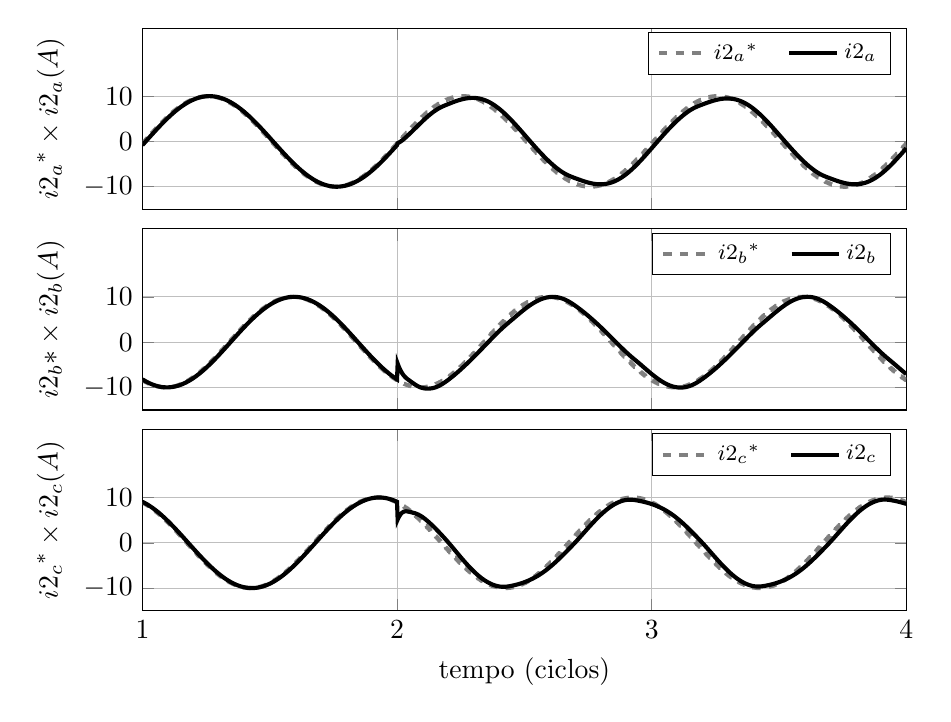
\begin{tikzpicture}

\begin{axis}[%
width=0.8\textwidth,
height=0.189701500343624\textwidth,
scale only axis,
xmin=0.316666666666667,
xmax=0.366666666666667,
xtick={0.316666666666667,0.333333333333333,0.35,0.366666666666667},
xticklabels={\empty},
xmajorgrids,
ymin=-15,
ymax=25,
ytick={-10,   0,  10},
ylabel={${\text{i2}_\text{b}}\text{* }\times\text{ i2}_\text{b}\text{ (A)}$},
ymajorgrids,
name=plot2,
legend style={draw=black,fill=white,legend cell align=left},
scaled x ticks = false,
legend columns=-1,
legend style={/tikz/every even column/.append style={column sep=0.3cm}},
legend style={font=\footnotesize}
]
\addplot [color=gray,dashed,line width=1.5pt]
  table[row sep=crcr]{0.316658333333333	-8.32921240710225\\
0.3167	-8.49892692986993\\
0.316741666666667	-8.49892692986993\\
0.316783333333333	-8.6602540378457\\
0.316825	-8.6602540378457\\
0.316866666666667	-8.81303452065127\\
0.316908333333333	-8.81303452065127\\
0.31695	-8.9571176023955\\
0.316991666666667	-8.9571176023955\\
0.317033333333333	-9.09236109047209\\
0.317075	-9.09236109047209\\
0.317116666666667	-9.21863151588643\\
0.317158333333333	-9.21863151588643\\
0.3172	-9.33580426497347\\
0.317241666666667	-9.33580426497347\\
0.317283333333333	-9.44376370237628\\
0.317325	-9.44376370237628\\
0.317366666666667	-9.54240328516426\\
0.317408333333333	-9.54240328516426\\
0.31745	-9.63162566797809\\
0.317491666666667	-9.63162566797809\\
0.317533333333333	-9.71134279909789\\
0.317575	-9.71134279909789\\
0.317616666666667	-9.7814760073396\\
0.317658333333333	-9.7814760073396\\
0.3177	-9.84195607969398\\
0.317741666666667	-9.84195607969398\\
0.317783333333333	-9.89272332963145\\
0.317825	-9.89272332963145\\
0.317866666666667	-9.93372765600555\\
0.317908333333333	-9.93372765600555\\
0.31795	-9.96492859249664\\
0.317991666666667	-9.96492859249664\\
0.318033333333333	-9.98629534754734\\
0.318075	-9.98629534754734\\
0.318116666666667	-9.99780683475006\\
0.318158333333333	-9.99780683475006\\
0.3182	-9.99945169365673\\
0.318241666666667	-9.99945169365673\\
0.318283333333333	-9.9912283009902\\
0.318325	-9.9912283009902\\
0.318366666666667	-9.9731447722462\\
0.318408333333333	-9.9731447722462\\
0.31845	-9.94521895368435\\
0.318491666666667	-9.94521895368435\\
0.318533333333333	-9.90747840471606\\
0.318575	-9.90747840471606\\
0.318616666666667	-9.85996037070666\\
0.318658333333333	-9.85996037070666\\
0.3187	-9.80271174621883\\
0.318741666666667	-9.80271174621883\\
0.318783333333333	-9.73578902873321\\
0.318825	-9.73578902873321\\
0.318866666666667	-9.65925826289228\\
0.318908333333333	-9.65925826289228\\
0.31895	-9.57319497532226\\
0.318991666666667	-9.57319497532226\\
0.319033333333333	-9.47768410009743\\
0.319075	-9.47768410009743\\
0.319116666666667	-9.37281989492048\\
0.319158333333333	-9.37281989492048\\
0.3192	-9.2587058481015\\
0.319241666666667	-9.2587058481015\\
0.319283333333333	-9.13545457642755\\
0.319325	-9.13545457642755\\
0.319366666666667	-9.00318771402345\\
0.319408333333333	-9.00318771402345\\
0.31945	-8.86203579231365\\
0.319491666666667	-8.86203579231365\\
0.319533333333333	-8.71213811120338\\
0.319575	-8.71213811120338\\
0.319616666666667	-8.55364260160653\\
0.319658333333333	-8.55364260160653\\
0.3197	-8.38670567945568\\
0.319741666666667	-8.38670567945568\\
0.319783333333333	-8.21149209133845\\
0.319825	-8.21149209133845\\
0.319866666666667	-8.02817475191253\\
0.319908333333333	-8.02817475191253\\
0.31995	-7.83693457325976\\
0.319991666666667	-7.83693457325976\\
0.320033333333333	-7.63796028634775\\
0.320075	-7.63796028634775\\
0.320116666666667	-7.43144825477524\\
0.320158333333333	-7.43144825477524\\
0.3202	-7.21760228098489\\
0.320241666666667	-7.21760228098489\\
0.320283333333333	-6.99663340513489\\
0.320325	-6.99663340513489\\
0.320366666666667	-6.76875969682781\\
0.320408333333333	-6.76875969682781\\
0.32045	-6.53420603990222\\
0.320491666666667	-6.53420603990222\\
0.320533333333333	-6.29320391049951\\
0.320575	-6.29320391049951\\
0.320616666666667	-6.04599114862485\\
0.320658333333333	-6.04599114862485\\
0.3207	-5.79281172342785\\
0.320741666666667	-5.79281172342785\\
0.320783333333333	-5.53391549243446\\
0.320825	-5.53391549243446\\
0.320866666666667	-5.26955795496776\\
0.320908333333333	-5.26955795496776\\
0.32095	-5.00000000000094\\
0.320991666666667	-5.00000000000094\\
0.321033333333333	-4.72550764869144\\
0.321075	-4.72550764869144\\
0.321116666666667	-4.44635179185013\\
0.321158333333333	-4.44635179185013\\
0.3212	-4.16280792260482\\
0.321241666666667	-4.16280792260482\\
0.321283333333333	-3.87515586452179\\
0.321325	-3.87515586452179\\
0.321366666666667	-3.58367949545372\\
0.321408333333333	-3.58367949545372\\
0.32145	-3.28866646738651\\
0.321491666666667	-3.28866646738651\\
0.321533333333333	-2.99040792256149\\
0.321575	-2.99040792256149\\
0.321616666666667	-2.68919820615324\\
0.321658333333333	-2.68919820615324\\
0.3217	-2.38533457578634\\
0.321741666666667	-2.38533457578634\\
0.321783333333333	-2.07911690817807\\
0.321825	-2.07911690817807\\
0.321866666666667	-1.77084740319627\\
0.321908333333333	-1.77084740319627\\
0.32195	-1.4608302856245\\
0.321991666666667	-1.4608302856245\\
0.322033333333333	-1.149371504929\\
0.322075	-1.149371504929\\
0.322116666666667	-0.836778433323436\\
0.322158333333333	-0.836778433323436\\
0.3222	-0.523359562429668\\
0.322241666666667	-0.523359562429668\\
0.322283333333333	-0.209424198833749\\
0.322325	-0.209424198833749\\
0.322366666666667	0.10471784116233\\
0.322408333333333	0.10471784116233\\
0.32245	0.41875653729192\\
0.322491666666667	0.41875653729192\\
0.322533333333333	0.732381971276291\\
0.322575	0.732381971276291\\
0.322616666666667	1.04528463267656\\
0.322658333333333	1.04528463267656\\
0.3227	1.35715572434312\\
0.322741666666667	1.35715572434312\\
0.322783333333333	1.66768746716115\\
0.322825	1.66768746716115\\
0.322866666666667	1.97657340379144\\
0.322908333333333	1.97657340379144\\
0.32295	2.28350870110679\\
0.322991666666667	2.28350870110679\\
0.323033333333333	2.58819045102549\\
0.323075	2.58819045102549\\
0.323116666666667	2.89031796944505\\
0.323158333333333	2.89031796944505\\
0.3232	3.18959309298109\\
0.323241666666667	3.18959309298109\\
0.323283333333333	3.48572047321859\\
0.323325	3.48572047321859\\
0.323366666666667	3.77840786818516\\
0.323408333333333	3.77840786818516\\
0.32345	4.06736643075854\\
0.323491666666667	4.06736643075854\\
0.323533333333333	4.35231099372386\\
0.323575	4.35231099372386\\
0.323616666666667	4.63296035119925\\
0.323658333333333	4.63296035119925\\
0.3237	4.90903753615209\\
0.323741666666667	4.90903753615209\\
0.323783333333333	5.18027009373203\\
0.323825	5.18027009373203\\
0.323866666666667	5.44639035015104\\
0.323908333333333	5.44639035015104\\
0.32395	5.70713567684513\\
0.323991666666667	5.70713567684513\\
0.324033333333333	5.96224874965702\\
0.324075	5.96224874965702\\
0.324116666666667	6.21147780278401\\
0.324158333333333	6.21147780278401\\
0.3242	6.45457687724046\\
0.324241666666667	6.45457687724046\\
0.324283333333333	6.69130606358958\\
0.324325	6.69130606358958\\
0.324366666666667	6.9214317387051\\
0.324408333333333	6.9214317387051\\
0.32445	7.14472679632911\\
0.324491666666667	7.14472679632911\\
0.324533333333333	7.36097087119846\\
0.324575	7.36097087119846\\
0.324616666666667	7.56995055651872\\
0.324658333333333	7.56995055651872\\
0.3247	7.7714596145709\\
0.324741666666667	7.7714596145709\\
0.324783333333333	7.96529918024319\\
0.324825	7.96529918024319\\
0.324866666666667	8.1512779572868\\
0.324908333333333	8.1512779572868\\
0.32495	8.32921240710229\\
0.324991666666667	8.32921240710229\\
0.325033333333333	8.49892692986996\\
0.325075	8.49892692986996\\
0.325116666666667	8.66025403784574\\
0.325158333333333	8.66025403784574\\
0.3252	8.81303452065131\\
0.325241666666667	8.81303452065131\\
0.325283333333333	8.95711760239554\\
0.325325	8.95711760239554\\
0.325366666666667	9.09236109047212\\
0.325408333333333	9.09236109047212\\
0.32545	9.21863151588647\\
0.325491666666667	9.21863151588647\\
0.325533333333333	9.33580426497351\\
0.325575	9.33580426497351\\
0.325616666666667	9.44376370237632\\
0.325658333333333	9.44376370237632\\
0.3257	9.5424032851643\\
0.325741666666667	9.5424032851643\\
0.325783333333333	9.63162566797813\\
0.325825	9.63162566797813\\
0.325866666666667	9.71134279909793\\
0.325908333333333	9.71134279909793\\
0.32595	9.78147600733964\\
0.325991666666667	9.78147600733964\\
0.326033333333333	9.84195607969402\\
0.326075	9.84195607969402\\
0.326116666666667	9.8927233296315\\
0.326158333333333	9.8927233296315\\
0.3262	9.93372765600559\\
0.326241666666667	9.93372765600559\\
0.326283333333333	9.96492859249668\\
0.326325	9.96492859249668\\
0.326366666666667	9.98629534754738\\
0.326408333333333	9.98629534754738\\
0.32645	9.99780683475011\\
0.326491666666667	9.99780683475011\\
0.326533333333333	9.99945169365678\\
0.326575	9.99945169365678\\
0.326616666666667	9.99122830099025\\
0.326658333333333	9.99122830099025\\
0.3267	9.97314477224624\\
0.326741666666667	9.97314477224624\\
0.326783333333333	9.9452189536844\\
0.326825	9.9452189536844\\
0.326866666666667	9.9074784047161\\
0.326908333333333	9.9074784047161\\
0.32695	9.85996037070671\\
0.326991666666667	9.85996037070671\\
0.327033333333333	9.80271174621887\\
0.327075	9.80271174621887\\
0.327116666666667	9.73578902873325\\
0.327158333333333	9.73578902873325\\
0.3272	9.65925826289232\\
0.327241666666667	9.65925826289232\\
0.327283333333333	9.5731949753223\\
0.327325	9.5731949753223\\
0.327366666666667	9.47768410009748\\
0.327408333333333	9.47768410009748\\
0.32745	9.37281989492053\\
0.327491666666667	9.37281989492053\\
0.327533333333333	9.25870584810154\\
0.327575	9.25870584810154\\
0.327616666666667	9.13545457642759\\
0.327658333333333	9.13545457642759\\
0.3277	9.0031877140235\\
0.327741666666667	9.0031877140235\\
0.327783333333333	8.86203579231369\\
0.327825	8.86203579231369\\
0.327866666666667	8.71213811120342\\
0.327908333333333	8.71213811120342\\
0.32795	8.55364260160657\\
0.327991666666667	8.55364260160657\\
0.328033333333333	8.38670567945572\\
0.328075	8.38670567945572\\
0.328116666666667	8.21149209133849\\
0.328158333333333	8.21149209133849\\
0.3282	8.02817475191257\\
0.328241666666667	8.02817475191257\\
0.328283333333333	7.83693457325979\\
0.328325	7.83693457325979\\
0.328366666666667	7.63796028634779\\
0.328408333333333	7.63796028634779\\
0.32845	7.43144825477528\\
0.328491666666667	7.43144825477528\\
0.328533333333333	7.21760228098492\\
0.328575	7.21760228098492\\
0.328616666666667	6.99663340513492\\
0.328658333333333	6.99663340513492\\
0.3287	6.76875969682784\\
0.328741666666667	6.76875969682784\\
0.328783333333333	6.53420603990226\\
0.328825	6.53420603990226\\
0.328866666666667	6.29320391049954\\
0.328908333333333	6.29320391049954\\
0.32895	6.04599114862488\\
0.328991666666667	6.04599114862488\\
0.329033333333333	5.79281172342788\\
0.329075	5.79281172342788\\
0.329116666666667	5.53391549243449\\
0.329158333333333	5.53391549243449\\
0.3292	5.26955795496778\\
0.329241666666667	5.26955795496778\\
0.329283333333333	5.00000000000096\\
0.329325	5.00000000000096\\
0.329366666666667	4.72550764869146\\
0.329408333333333	4.72550764869146\\
0.32945	4.44635179185015\\
0.329491666666667	4.44635179185015\\
0.329533333333333	4.16280792260484\\
0.329575	4.16280792260484\\
0.329616666666667	3.87515586452181\\
0.329658333333333	3.87515586452181\\
0.3297	3.58367949545374\\
0.329741666666667	3.58367949545374\\
0.329783333333333	3.28866646738652\\
0.329825	3.28866646738652\\
0.329866666666667	2.99040792256151\\
0.329908333333333	2.99040792256151\\
0.32995	2.68919820615325\\
0.329991666666667	2.68919820615325\\
0.330033333333333	2.38533457578635\\
0.330075	2.38533457578635\\
0.330116666666667	2.07911690817808\\
0.330158333333333	2.07911690817808\\
0.3302	1.77084740319627\\
0.330241666666667	1.77084740319627\\
0.330283333333333	1.4608302856245\\
0.330325	1.4608302856245\\
0.330366666666667	1.149371504929\\
0.330408333333333	1.149371504929\\
0.33045	0.836778433323441\\
0.330491666666667	0.836778433323441\\
0.330533333333333	0.523359562429672\\
0.330575	0.523359562429672\\
0.330616666666667	0.20942419883375\\
0.330658333333333	0.20942419883375\\
0.3307	-0.10471784116233\\
0.330741666666667	-0.10471784116233\\
0.330783333333333	-0.418756537291922\\
0.330825	-0.418756537291922\\
0.330866666666667	-0.732381971276294\\
0.330908333333333	-0.732381971276294\\
0.33095	-1.04528463267656\\
0.330991666666667	-1.04528463267656\\
0.331033333333333	-1.35715572434313\\
0.331075	-1.35715572434313\\
0.331116666666667	-1.66768746716116\\
0.331158333333333	-1.66768746716116\\
0.3312	-1.97657340379145\\
0.331241666666667	-1.97657340379145\\
0.331283333333333	-2.2835087011068\\
0.331325	-2.2835087011068\\
0.331366666666667	-2.5881904510255\\
0.331408333333333	-2.5881904510255\\
0.33145	-2.89031796944506\\
0.331491666666667	-2.89031796944506\\
0.331533333333333	-3.1895930929811\\
0.331575	-3.1895930929811\\
0.331616666666667	-3.4857204732186\\
0.331658333333333	-3.4857204732186\\
0.3317	-3.77840786818517\\
0.331741666666667	-3.77840786818517\\
0.331783333333333	-4.06736643075855\\
0.331825	-4.06736643075855\\
0.331866666666667	-4.35231099372388\\
0.331908333333333	-4.35231099372388\\
0.33195	-4.63296035119927\\
0.331991666666667	-4.63296035119927\\
0.332033333333333	-4.90903753615211\\
0.332075	-4.90903753615211\\
0.332116666666667	-5.18027009373205\\
0.332158333333333	-5.18027009373205\\
0.3322	-5.44639035015107\\
0.332241666666667	-5.44639035015107\\
0.332283333333333	-5.70713567684516\\
0.332325	-5.70713567684516\\
0.332366666666667	-5.96224874965705\\
0.332408333333333	-5.96224874965705\\
0.33245	-6.21147780278404\\
0.332491666666667	-6.21147780278404\\
0.332533333333333	-6.45457687724048\\
0.332575	-6.45457687724048\\
0.332616666666667	-6.6913060635896\\
0.332658333333333	-6.6913060635896\\
0.3327	-6.92143173870513\\
0.332741666666667	-6.92143173870513\\
0.332783333333333	-7.14472679632914\\
0.332825	-7.14472679632914\\
0.332866666666667	-7.36097087119849\\
0.332908333333333	-7.36097087119849\\
0.33295	-7.56995055651875\\
0.332991666666667	-7.56995055651875\\
0.333033333333333	-7.77145961457093\\
0.333075	-7.77145961457093\\
0.333116666666667	-7.96529918024322\\
0.333158333333333	-7.96529918024322\\
0.3332	-8.15127795728684\\
0.333241666666667	-8.15127795728684\\
0.333283333333333	-8.32921240710232\\
0.333325	-8.32921240710232\\
0.333366666666667	-8.49892692987\\
0.333408333333333	-8.49892692987\\
0.33345	-8.66025403784578\\
0.333491666666667	-8.66025403784578\\
0.333533333333333	-8.81303452065134\\
0.333575	-8.81303452065134\\
0.333616666666667	-8.95711760239558\\
0.333658333333333	-8.95711760239558\\
0.3337	-9.09236109047216\\
0.333741666666667	-9.09236109047216\\
0.333783333333333	-9.21863151588651\\
0.333825	-9.21863151588651\\
0.333866666666667	-9.33580426497354\\
0.333908333333333	-9.33580426497354\\
0.33395	-9.44376370237636\\
0.333991666666667	-9.44376370237636\\
0.334033333333333	-9.54240328516434\\
0.334075	-9.54240328516434\\
0.334116666666667	-9.63162566797817\\
0.334158333333333	-9.63162566797817\\
0.3342	-9.71134279909797\\
0.334241666666667	-9.71134279909797\\
0.334283333333333	-9.78147600733968\\
0.334325	-9.78147600733968\\
0.334366666666667	-9.84195607969406\\
0.334408333333333	-9.84195607969406\\
0.33445	-9.89272332963154\\
0.334491666666667	-9.89272332963154\\
0.334533333333333	-9.93372765600563\\
0.334575	-9.93372765600563\\
0.334616666666667	-9.96492859249672\\
0.334658333333333	-9.96492859249672\\
0.3347	-9.98629534754742\\
0.334741666666667	-9.98629534754742\\
0.334783333333333	-9.99780683475015\\
0.334825	-9.99780683475015\\
0.334866666666667	-9.99945169365682\\
0.334908333333333	-9.99945169365682\\
0.33495	-9.99122830099028\\
0.334991666666667	-9.99122830099028\\
0.335033333333333	-9.97314477224628\\
0.335075	-9.97314477224628\\
0.335116666666667	-9.94521895368444\\
0.335158333333333	-9.94521895368444\\
0.3352	-9.90747840471614\\
0.335241666666667	-9.90747840471614\\
0.335283333333333	-9.85996037070675\\
0.335325	-9.85996037070675\\
0.335366666666667	-9.80271174621891\\
0.335408333333333	-9.80271174621891\\
0.33545	-9.73578902873329\\
0.335491666666667	-9.73578902873329\\
0.335533333333333	-9.65925826289236\\
0.335575	-9.65925826289236\\
0.335616666666667	-9.57319497532234\\
0.335658333333333	-9.57319497532234\\
0.3357	-9.47768410009751\\
0.335741666666667	-9.47768410009751\\
0.335783333333333	-9.37281989492056\\
0.335825	-9.37281989492056\\
0.335866666666667	-9.25870584810158\\
0.335908333333333	-9.25870584810158\\
0.33595	-9.13545457642762\\
0.335991666666667	-9.13545457642762\\
0.336033333333333	-9.00318771402353\\
0.336075	-9.00318771402353\\
0.336116666666667	-8.86203579231372\\
0.336158333333333	-8.86203579231372\\
0.3362	-8.71213811120345\\
0.336241666666667	-8.71213811120345\\
0.336283333333333	-8.5536426016066\\
0.336325	-8.5536426016066\\
0.336366666666667	-8.38670567945575\\
0.336408333333333	-8.38670567945575\\
0.33645	-8.21149209133852\\
0.336491666666667	-8.21149209133852\\
0.336533333333333	-8.0281747519126\\
0.336575	-8.0281747519126\\
0.336616666666667	-7.83693457325982\\
0.336658333333333	-7.83693457325982\\
0.3367	-7.63796028634782\\
0.336741666666667	-7.63796028634782\\
0.336783333333333	-7.43144825477531\\
0.336825	-7.43144825477531\\
0.336866666666667	-7.21760228098495\\
0.336908333333333	-7.21760228098495\\
0.33695	-6.99663340513495\\
0.336991666666667	-6.99663340513495\\
0.337033333333333	-6.76875969682787\\
0.337075	-6.76875969682787\\
0.337116666666667	-6.53420603990228\\
0.337158333333333	-6.53420603990228\\
0.3372	-6.29320391049956\\
0.337241666666667	-6.29320391049956\\
0.337283333333333	-6.0459911486249\\
0.337325	-6.0459911486249\\
0.337366666666667	-5.7928117234279\\
0.337408333333333	-5.7928117234279\\
0.33745	-5.53391549243451\\
0.337491666666667	-5.53391549243451\\
0.337533333333333	-5.2695579549678\\
0.337575	-5.2695579549678\\
0.337616666666667	-5.00000000000098\\
0.337658333333333	-5.00000000000098\\
0.3377	-4.72550764869148\\
0.337741666666667	-4.72550764869148\\
0.337783333333333	-4.44635179185017\\
0.337825	-4.44635179185017\\
0.337866666666667	-4.16280792260486\\
0.337908333333333	-4.16280792260486\\
0.33795	-3.87515586452183\\
0.337991666666667	-3.87515586452183\\
0.338033333333333	-3.58367949545375\\
0.338075	-3.58367949545375\\
0.338116666666667	-3.28866646738653\\
0.338158333333333	-3.28866646738653\\
0.3382	-2.99040792256152\\
0.338241666666667	-2.99040792256152\\
0.338283333333333	-2.68919820615326\\
0.338325	-2.68919820615326\\
0.338366666666667	-2.38533457578636\\
0.338408333333333	-2.38533457578636\\
0.33845	-2.07911690817809\\
0.338491666666667	-2.07911690817809\\
0.338533333333333	-1.77084740319628\\
0.338575	-1.77084740319628\\
0.338616666666667	-1.46083028562451\\
0.338658333333333	-1.46083028562451\\
0.3387	-1.14937150492901\\
0.338741666666667	-1.14937150492901\\
0.338783333333333	-0.836778433323443\\
0.338825	-0.836778433323443\\
0.338866666666667	-0.523359562429674\\
0.338908333333333	-0.523359562429674\\
0.33895	-0.209424198833751\\
0.338991666666667	-0.209424198833751\\
0.339033333333333	0.104717841162331\\
0.339075	0.104717841162331\\
0.339116666666667	0.418756537291924\\
0.339158333333333	0.418756537291924\\
0.3392	0.732381971276298\\
0.339241666666667	0.732381971276298\\
0.339283333333333	1.04528463267657\\
0.339325	1.04528463267657\\
0.339366666666667	1.35715572434313\\
0.339408333333333	1.35715572434313\\
0.33945	1.66768746716117\\
0.339491666666667	1.66768746716117\\
0.339533333333333	1.97657340379146\\
0.339575	1.97657340379146\\
0.339616666666667	2.28350870110681\\
0.339658333333333	2.28350870110681\\
0.3397	2.58819045102551\\
0.339741666666667	2.58819045102551\\
0.339783333333333	2.89031796944507\\
0.339825	2.89031796944507\\
0.339866666666667	3.18959309298111\\
0.339908333333333	3.18959309298111\\
0.33995	3.48572047321862\\
0.339991666666667	3.48572047321862\\
0.340033333333333	3.77840786818519\\
0.340075	3.77840786818519\\
0.340116666666667	4.06736643075857\\
0.340158333333333	4.06736643075857\\
0.3402	4.35231099372389\\
0.340241666666667	4.35231099372389\\
0.340283333333333	4.63296035119929\\
0.340325	4.63296035119929\\
0.340366666666667	4.90903753615213\\
0.340408333333333	4.90903753615213\\
0.34045	5.18027009373207\\
0.340491666666667	5.18027009373207\\
0.340533333333333	5.44639035015109\\
0.340575	5.44639035015109\\
0.340616666666667	5.70713567684518\\
0.340658333333333	5.70713567684518\\
0.3407	5.96224874965707\\
0.340741666666667	5.96224874965707\\
0.340783333333333	6.21147780278406\\
0.340825	6.21147780278406\\
0.340866666666667	6.45457687724051\\
0.340908333333333	6.45457687724051\\
0.34095	6.69130606358963\\
0.340991666666667	6.69130606358963\\
0.341033333333333	6.92143173870516\\
0.341075	6.92143173870516\\
0.341116666666667	7.14472679632916\\
0.341158333333333	7.14472679632916\\
0.3412	7.36097087119851\\
0.341241666666667	7.36097087119851\\
0.341283333333333	7.56995055651877\\
0.341325	7.56995055651877\\
0.341366666666667	7.77145961457096\\
0.341408333333333	7.77145961457096\\
0.34145	7.96529918024325\\
0.341491666666667	7.96529918024325\\
0.341533333333333	8.15127795728687\\
0.341575	8.15127795728687\\
0.341616666666667	8.32921240710235\\
0.341658333333333	8.32921240710235\\
0.3417	8.49892692987003\\
0.341741666666667	8.49892692987003\\
0.341783333333333	8.66025403784581\\
0.341825	8.66025403784581\\
0.341866666666667	8.81303452065138\\
0.341908333333333	8.81303452065138\\
0.34195	8.95711760239561\\
0.341991666666667	8.95711760239561\\
0.342033333333333	9.0923610904722\\
0.342075	9.0923610904722\\
0.342116666666667	9.21863151588654\\
0.342158333333333	9.21863151588654\\
0.3422	9.33580426497358\\
0.342241666666667	9.33580426497358\\
0.342283333333333	9.4437637023764\\
0.342325	9.4437637023764\\
0.342366666666667	9.54240328516438\\
0.342408333333333	9.54240328516438\\
0.34245	9.63162566797821\\
0.342491666666667	9.63162566797821\\
0.342533333333333	9.71134279909801\\
0.342575	9.71134279909801\\
0.342616666666667	9.78147600733972\\
0.342658333333333	9.78147600733972\\
0.3427	9.8419560796941\\
0.342741666666667	9.8419560796941\\
0.342783333333333	9.89272332963157\\
0.342825	9.89272332963157\\
0.342866666666667	9.93372765600567\\
0.342908333333333	9.93372765600567\\
0.34295	9.96492859249676\\
0.342991666666667	9.96492859249676\\
0.343033333333333	9.98629534754746\\
0.343075	9.98629534754746\\
0.343116666666667	9.99780683475019\\
0.343158333333333	9.99780683475019\\
0.3432	9.99945169365686\\
0.343241666666667	9.99945169365686\\
0.343283333333333	9.99122830099032\\
0.343325	9.99122830099032\\
0.343366666666667	9.97314477224632\\
0.343408333333333	9.97314477224632\\
0.34345	9.94521895368448\\
0.343491666666667	9.94521895368448\\
0.343533333333333	9.90747840471618\\
0.343575	9.90747840471618\\
0.343616666666667	9.85996037070679\\
0.343658333333333	9.85996037070679\\
0.3437	9.80271174621895\\
0.343741666666667	9.80271174621895\\
0.343783333333333	9.73578902873333\\
0.343825	9.73578902873333\\
0.343866666666667	9.6592582628924\\
0.343908333333333	9.6592582628924\\
0.34395	9.57319497532238\\
0.343991666666667	9.57319497532238\\
0.344033333333333	9.47768410009755\\
0.344075	9.47768410009755\\
0.344116666666667	9.3728198949206\\
0.344158333333333	9.3728198949206\\
0.3442	9.25870584810162\\
0.344241666666667	9.25870584810162\\
0.344283333333333	9.13545457642766\\
0.344325	9.13545457642766\\
0.344366666666667	9.00318771402357\\
0.344408333333333	9.00318771402357\\
0.34445	8.86203579231376\\
0.344491666666667	8.86203579231376\\
0.344533333333333	8.71213811120348\\
0.344575	8.71213811120348\\
0.344616666666667	8.55364260160663\\
0.344658333333333	8.55364260160663\\
0.3447	8.38670567945578\\
0.344741666666667	8.38670567945578\\
0.344783333333333	8.21149209133855\\
0.344825	8.21149209133855\\
0.344866666666667	8.02817475191263\\
0.344908333333333	8.02817475191263\\
0.34495	7.83693457325986\\
0.344991666666667	7.83693457325986\\
0.345033333333333	7.63796028634785\\
0.345075	7.63796028634785\\
0.345116666666667	7.43144825477534\\
0.345158333333333	7.43144825477534\\
0.3452	7.21760228098498\\
0.345241666666667	7.21760228098498\\
0.345283333333333	6.99663340513498\\
0.345325	6.99663340513498\\
0.345366666666667	6.7687596968279\\
0.345408333333333	6.7687596968279\\
0.34545	6.5342060399023\\
0.345491666666667	6.5342060399023\\
0.345533333333333	6.29320391049959\\
0.345575	6.29320391049959\\
0.345616666666667	6.04599114862492\\
0.345658333333333	6.04599114862492\\
0.3457	5.79281172342792\\
0.345741666666667	5.79281172342792\\
0.345783333333333	5.53391549243453\\
0.345825	5.53391549243453\\
0.345866666666667	5.26955795496782\\
0.345908333333333	5.26955795496782\\
0.34595	5.000000000001\\
0.345991666666667	5.000000000001\\
0.346033333333333	4.72550764869149\\
0.346075	4.72550764869149\\
0.346116666666667	4.44635179185018\\
0.346158333333333	4.44635179185018\\
0.3462	4.16280792260487\\
0.346241666666667	4.16280792260487\\
0.346283333333333	3.87515586452184\\
0.346325	3.87515586452184\\
0.346366666666667	3.58367949545377\\
0.346408333333333	3.58367949545377\\
0.34645	3.28866646738655\\
0.346491666666667	3.28866646738655\\
0.346533333333333	2.99040792256153\\
0.346575	2.99040792256153\\
0.346616666666667	2.68919820615327\\
0.346658333333333	2.68919820615327\\
0.3467	2.38533457578637\\
0.346741666666667	2.38533457578637\\
0.346783333333333	2.0791169081781\\
0.346825	2.0791169081781\\
0.346866666666667	1.77084740319629\\
0.346908333333333	1.77084740319629\\
0.34695	1.46083028562452\\
0.346991666666667	1.46083028562452\\
0.347033333333333	1.14937150492901\\
0.347075	1.14937150492901\\
0.347116666666667	0.836778433323448\\
0.347158333333333	0.836778433323448\\
0.3472	0.523359562429677\\
0.347241666666667	0.523359562429677\\
0.347283333333333	0.209424198833753\\
0.347325	0.209424198833753\\
0.347366666666667	-0.10471784116233\\
0.347408333333333	-0.10471784116233\\
0.34745	-0.418756537291923\\
0.347491666666667	-0.418756537291923\\
0.347533333333333	-0.732381971276299\\
0.347575	-0.732381971276299\\
0.347616666666667	-1.04528463267657\\
0.347658333333333	-1.04528463267657\\
0.3477	-1.35715572434314\\
0.347741666666667	-1.35715572434314\\
0.347783333333333	-1.66768746716117\\
0.347825	-1.66768746716117\\
0.347866666666667	-1.97657340379147\\
0.347908333333333	-1.97657340379147\\
0.34795	-2.28350870110682\\
0.347991666666667	-2.28350870110682\\
0.348033333333333	-2.58819045102552\\
0.348075	-2.58819045102552\\
0.348116666666667	-2.89031796944508\\
0.348158333333333	-2.89031796944508\\
0.3482	-3.18959309298112\\
0.348241666666667	-3.18959309298112\\
0.348283333333333	-3.48572047321863\\
0.348325	-3.48572047321863\\
0.348366666666667	-3.7784078681852\\
0.348408333333333	-3.7784078681852\\
0.34845	-4.06736643075858\\
0.348491666666667	-4.06736643075858\\
0.348533333333333	-4.35231099372391\\
0.348575	-4.35231099372391\\
0.348616666666667	-4.6329603511993\\
0.348658333333333	-4.6329603511993\\
0.3487	-4.90903753615215\\
0.348741666666667	-4.90903753615215\\
0.348783333333333	-5.18027009373209\\
0.348825	-5.18027009373209\\
0.348866666666667	-5.44639035015111\\
0.348908333333333	-5.44639035015111\\
0.34895	-5.7071356768452\\
0.348991666666667	-5.7071356768452\\
0.349033333333333	-5.96224874965709\\
0.349075	-5.96224874965709\\
0.349116666666667	-6.21147780278408\\
0.349158333333333	-6.21147780278408\\
0.3492	-6.45457687724053\\
0.349241666666667	-6.45457687724053\\
0.349283333333333	-6.69130606358966\\
0.349325	-6.69130606358966\\
0.349366666666667	-6.92143173870518\\
0.349408333333333	-6.92143173870518\\
0.34945	-7.14472679632919\\
0.349491666666667	-7.14472679632919\\
0.349533333333333	-7.36097087119854\\
0.349575	-7.36097087119854\\
0.349616666666667	-7.5699505565188\\
0.349658333333333	-7.5699505565188\\
0.3497	-7.77145961457099\\
0.349741666666667	-7.77145961457099\\
0.349783333333333	-7.96529918024328\\
0.349825	-7.96529918024328\\
0.349866666666667	-8.1512779572869\\
0.349908333333333	-8.1512779572869\\
0.34995	-8.32921240710239\\
0.349991666666667	-8.32921240710239\\
0.350033333333333	-8.49892692987007\\
0.350075	-8.49892692987007\\
0.350116666666667	-8.66025403784585\\
0.350158333333333	-8.66025403784585\\
0.3502	-8.81303452065141\\
0.350241666666667	-8.81303452065141\\
0.350283333333333	-8.95711760239565\\
0.350325	-8.95711760239565\\
0.350366666666667	-9.09236109047223\\
0.350408333333333	-9.09236109047223\\
0.35045	-9.21863151588658\\
0.350491666666667	-9.21863151588658\\
0.350533333333333	-9.33580426497362\\
0.350575	-9.33580426497362\\
0.350616666666667	-9.44376370237644\\
0.350658333333333	-9.44376370237644\\
0.3507	-9.54240328516442\\
0.350741666666667	-9.54240328516442\\
0.350783333333333	-9.63162566797825\\
0.350825	-9.63162566797825\\
0.350866666666667	-9.71134279909805\\
0.350908333333333	-9.71134279909805\\
0.35095	-9.78147600733976\\
0.350991666666667	-9.78147600733976\\
0.351033333333333	-9.84195607969414\\
0.351075	-9.84195607969414\\
0.351116666666667	-9.89272332963162\\
0.351158333333333	-9.89272332963162\\
0.3512	-9.93372765600571\\
0.351241666666667	-9.93372765600571\\
0.351283333333333	-9.9649285924968\\
0.351325	-9.9649285924968\\
0.351366666666667	-9.98629534754751\\
0.351408333333333	-9.98629534754751\\
0.35145	-9.99780683475023\\
0.351491666666667	-9.99780683475023\\
0.351533333333333	-9.9994516936569\\
0.351575	-9.9994516936569\\
0.351616666666667	-9.99122830099037\\
0.351658333333333	-9.99122830099037\\
0.3517	-9.97314477224637\\
0.351741666666667	-9.97314477224637\\
0.351783333333333	-9.94521895368452\\
0.351825	-9.94521895368452\\
0.351866666666667	-9.90747840471622\\
0.351908333333333	-9.90747840471622\\
0.35195	-9.85996037070683\\
0.351991666666667	-9.85996037070683\\
0.352033333333333	-9.80271174621899\\
0.352075	-9.80271174621899\\
0.352116666666667	-9.73578902873337\\
0.352158333333333	-9.73578902873337\\
0.3522	-9.65925826289244\\
0.352241666666667	-9.65925826289244\\
0.352283333333333	-9.57319497532242\\
0.352325	-9.57319497532242\\
0.352366666666667	-9.4776841000976\\
0.352408333333333	-9.4776841000976\\
0.35245	-9.37281989492064\\
0.352491666666667	-9.37281989492064\\
0.352533333333333	-9.25870584810166\\
0.352575	-9.25870584810166\\
0.352616666666667	-9.1354545764277\\
0.352658333333333	-9.1354545764277\\
0.3527	-9.00318771402361\\
0.352741666666667	-9.00318771402361\\
0.352783333333333	-8.8620357923138\\
0.352825	-8.8620357923138\\
0.352866666666667	-8.71213811120352\\
0.352908333333333	-8.71213811120352\\
0.35295	-8.55364260160667\\
0.352991666666667	-8.55364260160667\\
0.353033333333333	-8.38670567945582\\
0.353075	-8.38670567945582\\
0.353116666666667	-8.21149209133859\\
0.353158333333333	-8.21149209133859\\
0.3532	-8.02817475191267\\
0.353241666666667	-8.02817475191267\\
0.353283333333333	-7.83693457325989\\
0.353325	-7.83693457325989\\
0.353366666666667	-7.63796028634788\\
0.353408333333333	-7.63796028634788\\
0.35345	-7.43144825477537\\
0.353491666666667	-7.43144825477537\\
0.353533333333333	-7.21760228098502\\
0.353575	-7.21760228098502\\
0.353616666666667	-6.99663340513501\\
0.353658333333333	-6.99663340513501\\
0.3537	-6.76875969682793\\
0.353741666666667	-6.76875969682793\\
0.353783333333333	-6.53420603990234\\
0.353825	-6.53420603990234\\
0.353866666666667	-6.29320391049962\\
0.353908333333333	-6.29320391049962\\
0.35395	-6.04599114862495\\
0.353991666666667	-6.04599114862495\\
0.354033333333333	-5.79281172342795\\
0.354075	-5.79281172342795\\
0.354116666666667	-5.53391549243456\\
0.354158333333333	-5.53391549243456\\
0.3542	-5.26955795496785\\
0.354241666666667	-5.26955795496785\\
0.354283333333333	-5.00000000000103\\
0.354325	-5.00000000000103\\
0.354366666666667	-4.72550764869152\\
0.354408333333333	-4.72550764869152\\
0.35445	-4.44635179185021\\
0.354491666666667	-4.44635179185021\\
0.354533333333333	-4.16280792260489\\
0.354575	-4.16280792260489\\
0.354616666666667	-3.87515586452186\\
0.354658333333333	-3.87515586452186\\
0.3547	-3.58367949545379\\
0.354741666666667	-3.58367949545379\\
0.354783333333333	-3.28866646738657\\
0.354825	-3.28866646738657\\
0.354866666666667	-2.99040792256155\\
0.354908333333333	-2.99040792256155\\
0.35495	-2.68919820615329\\
0.354991666666667	-2.68919820615329\\
0.355033333333333	-2.38533457578638\\
0.355075	-2.38533457578638\\
0.355116666666667	-2.07911690817811\\
0.355158333333333	-2.07911690817811\\
0.3552	-1.7708474031963\\
0.355241666666667	-1.7708474031963\\
0.355283333333333	-1.46083028562453\\
0.355325	-1.46083028562453\\
0.355366666666667	-1.14937150492902\\
0.355408333333333	-1.14937150492902\\
0.35545	-0.836778433323456\\
0.355491666666667	-0.836778433323456\\
0.355533333333333	-0.523359562429684\\
0.355575	-0.523359562429684\\
0.355616666666667	-0.209424198833759\\
0.355658333333333	-0.209424198833759\\
0.3557	0.104717841162325\\
0.355741666666667	0.104717841162325\\
0.355783333333333	0.418756537291921\\
0.355825	0.418756537291921\\
0.355866666666667	0.732381971276297\\
0.355908333333333	0.732381971276297\\
0.35595	1.04528463267657\\
0.355991666666667	1.04528463267657\\
0.356033333333333	1.35715572434314\\
0.356075	1.35715572434314\\
0.356116666666667	1.66768746716117\\
0.356158333333333	1.66768746716117\\
0.3562	1.97657340379147\\
0.356241666666667	1.97657340379147\\
0.356283333333333	2.28350870110682\\
0.356325	2.28350870110682\\
0.356366666666667	2.58819045102553\\
0.356408333333333	2.58819045102553\\
0.35645	2.89031796944509\\
0.356491666666667	2.89031796944509\\
0.356533333333333	3.18959309298113\\
0.356575	3.18959309298113\\
0.356616666666667	3.48572047321864\\
0.356658333333333	3.48572047321864\\
0.3567	3.77840786818521\\
0.356741666666667	3.77840786818521\\
0.356783333333333	4.0673664307586\\
0.356825	4.0673664307586\\
0.356866666666667	4.35231099372392\\
0.356908333333333	4.35231099372392\\
0.35695	4.63296035119932\\
0.356991666666667	4.63296035119932\\
0.357033333333333	4.90903753615216\\
0.357075	4.90903753615216\\
0.357116666666667	5.18027009373211\\
0.357158333333333	5.18027009373211\\
0.3572	5.44639035015113\\
0.357241666666667	5.44639035015113\\
0.357283333333333	5.70713567684522\\
0.357325	5.70713567684522\\
0.357366666666667	5.96224874965711\\
0.357408333333333	5.96224874965711\\
0.35745	6.21147780278411\\
0.357491666666667	6.21147780278411\\
0.357533333333333	6.45457687724056\\
0.357575	6.45457687724056\\
0.357616666666667	6.69130606358968\\
0.357658333333333	6.69130606358968\\
0.3577	6.92143173870521\\
0.357741666666667	6.92143173870521\\
0.357783333333333	7.14472679632922\\
0.357825	7.14472679632922\\
0.357866666666667	7.36097087119857\\
0.357908333333333	7.36097087119857\\
0.35795	7.56995055651883\\
0.357991666666667	7.56995055651883\\
0.358033333333333	7.77145961457102\\
0.358075	7.77145961457102\\
0.358116666666667	7.96529918024331\\
0.358158333333333	7.96529918024331\\
0.3582	8.15127795728693\\
0.358241666666667	8.15127795728693\\
0.358283333333333	8.32921240710242\\
0.358325	8.32921240710242\\
0.358366666666667	8.4989269298701\\
0.358408333333333	8.4989269298701\\
0.35845	8.66025403784588\\
0.358491666666667	8.66025403784588\\
0.358533333333333	8.81303452065145\\
0.358575	8.81303452065145\\
0.358616666666667	8.95711760239568\\
0.358658333333333	8.95711760239568\\
0.3587	9.09236109047227\\
0.358741666666667	9.09236109047227\\
0.358783333333333	9.21863151588662\\
0.358825	9.21863151588662\\
0.358866666666667	9.33580426497366\\
0.358908333333333	9.33580426497366\\
0.35895	9.44376370237647\\
0.358991666666667	9.44376370237647\\
0.359033333333333	9.54240328516445\\
0.359075	9.54240328516445\\
0.359116666666667	9.63162566797829\\
0.359158333333333	9.63162566797829\\
0.3592	9.71134279909809\\
0.359241666666667	9.71134279909809\\
0.359283333333333	9.7814760073398\\
0.359325	9.7814760073398\\
0.359366666666667	9.84195607969418\\
0.359408333333333	9.84195607969418\\
0.35945	9.89272332963166\\
0.359491666666667	9.89272332963166\\
0.359533333333333	9.93372765600575\\
0.359575	9.93372765600575\\
0.359616666666667	9.96492859249684\\
0.359658333333333	9.96492859249684\\
0.3597	9.98629534754755\\
0.359741666666667	9.98629534754755\\
0.359783333333333	9.99780683475027\\
0.359825	9.99780683475027\\
0.359866666666667	9.99945169365694\\
0.359908333333333	9.99945169365694\\
0.35995	9.99122830099041\\
0.359991666666667	9.99122830099041\\
0.360033333333333	9.97314477224641\\
0.360075	9.97314477224641\\
0.360116666666667	9.94521895368456\\
0.360158333333333	9.94521895368456\\
0.3602	9.90747840471626\\
0.360241666666667	9.90747840471626\\
0.360283333333333	9.85996037070687\\
0.360325	9.85996037070687\\
0.360366666666667	9.80271174621904\\
0.360408333333333	9.80271174621904\\
0.36045	9.73578902873341\\
0.360491666666667	9.73578902873341\\
0.360533333333333	9.65925826289248\\
0.360575	9.65925826289248\\
0.360616666666667	9.57319497532246\\
0.360658333333333	9.57319497532246\\
0.3607	9.47768410009764\\
0.360741666666667	9.47768410009764\\
0.360783333333333	9.37281989492068\\
0.360825	9.37281989492068\\
0.360866666666667	9.25870584810169\\
0.360908333333333	9.25870584810169\\
0.36095	9.13545457642774\\
0.360991666666667	9.13545457642774\\
0.361033333333333	9.00318771402364\\
0.361075	9.00318771402364\\
0.361116666666667	8.86203579231383\\
0.361158333333333	8.86203579231383\\
0.3612	8.71213811120356\\
0.361241666666667	8.71213811120356\\
0.361283333333333	8.55364260160671\\
0.361325	8.55364260160671\\
0.361366666666667	8.38670567945586\\
0.361408333333333	8.38670567945586\\
0.36145	8.21149209133863\\
0.361491666666667	8.21149209133863\\
0.361533333333333	8.0281747519127\\
0.361575	8.0281747519127\\
0.361616666666667	7.83693457325993\\
0.361658333333333	7.83693457325993\\
0.3617	7.63796028634792\\
0.361741666666667	7.63796028634792\\
0.361783333333333	7.4314482547754\\
0.361825	7.4314482547754\\
0.361866666666667	7.21760228098505\\
0.361908333333333	7.21760228098505\\
0.36195	6.99663340513504\\
0.361991666666667	6.99663340513504\\
0.362033333333333	6.76875969682796\\
0.362075	6.76875969682796\\
0.362116666666667	6.53420603990237\\
0.362158333333333	6.53420603990237\\
0.3622	6.29320391049965\\
0.362241666666667	6.29320391049965\\
0.362283333333333	6.04599114862498\\
0.362325	6.04599114862498\\
0.362366666666667	5.79281172342797\\
0.362408333333333	5.79281172342797\\
0.36245	5.53391549243458\\
0.362491666666667	5.53391549243458\\
0.362533333333333	5.26955795496787\\
0.362575	5.26955795496787\\
0.362616666666667	5.00000000000105\\
0.362658333333333	5.00000000000105\\
0.3627	4.72550764869154\\
0.362741666666667	4.72550764869154\\
0.362783333333333	4.44635179185023\\
0.362825	4.44635179185023\\
0.362866666666667	4.16280792260491\\
0.362908333333333	4.16280792260491\\
0.36295	3.87515586452188\\
0.362991666666667	3.87515586452188\\
0.363033333333333	3.5836794954538\\
0.363075	3.5836794954538\\
0.363116666666667	3.28866646738658\\
0.363158333333333	3.28866646738658\\
0.3632	2.99040792256156\\
0.363241666666667	2.99040792256156\\
0.363283333333333	2.6891982061533\\
0.363325	2.6891982061533\\
0.363366666666667	2.3853345757864\\
0.363408333333333	2.3853345757864\\
0.36345	2.07911690817813\\
0.363491666666667	2.07911690817813\\
0.363533333333333	1.77084740319631\\
0.363575	1.77084740319631\\
0.363616666666667	1.46083028562454\\
0.363658333333333	1.46083028562454\\
0.3637	1.14937150492903\\
0.363741666666667	1.14937150492903\\
0.363783333333333	0.836778433323463\\
0.363825	0.836778433323463\\
0.363866666666667	0.52335956242969\\
0.363908333333333	0.52335956242969\\
0.36395	0.209424198833764\\
0.363991666666667	0.209424198833764\\
0.364033333333333	-0.10471784116232\\
0.364075	-0.10471784116232\\
0.364116666666667	-0.418756537291917\\
0.364158333333333	-0.418756537291917\\
0.3642	-0.732381971276296\\
0.364241666666667	-0.732381971276296\\
0.364283333333333	-1.04528463267657\\
0.364325	-1.04528463267657\\
0.364366666666667	-1.35715572434314\\
0.364408333333333	-1.35715572434314\\
0.36445	-1.66768746716118\\
0.364491666666667	-1.66768746716118\\
0.364533333333333	-1.97657340379147\\
0.364575	-1.97657340379147\\
0.364616666666667	-2.28350870110683\\
0.364658333333333	-2.28350870110683\\
0.3647	-2.58819045102553\\
0.364741666666667	-2.58819045102553\\
0.364783333333333	-2.8903179694451\\
0.364825	-2.8903179694451\\
0.364866666666667	-3.18959309298114\\
0.364908333333333	-3.18959309298114\\
0.36495	-3.48572047321865\\
0.364991666666667	-3.48572047321865\\
0.365033333333333	-3.77840786818522\\
0.365075	-3.77840786818522\\
0.365116666666667	-4.06736643075861\\
0.365158333333333	-4.06736643075861\\
0.3652	-4.35231099372394\\
0.365241666666667	-4.35231099372394\\
0.365283333333333	-4.63296035119933\\
0.365325	-4.63296035119933\\
0.365366666666667	-4.90903753615218\\
0.365408333333333	-4.90903753615218\\
0.36545	-5.18027009373212\\
0.365491666666667	-5.18027009373212\\
0.365533333333333	-5.44639035015114\\
0.365575	-5.44639035015114\\
0.365616666666667	-5.70713567684524\\
0.365658333333333	-5.70713567684524\\
0.3657	-5.96224874965713\\
0.365741666666667	-5.96224874965713\\
0.365783333333333	-6.21147780278413\\
0.365825	-6.21147780278413\\
0.365866666666667	-6.45457687724057\\
0.365908333333333	-6.45457687724057\\
0.36595	-6.6913060635897\\
0.365991666666667	-6.6913060635897\\
0.366033333333333	-6.92143173870523\\
0.366075	-6.92143173870523\\
0.366116666666667	-7.14472679632924\\
0.366158333333333	-7.14472679632924\\
0.3662	-7.36097087119859\\
0.366241666666667	-7.36097087119859\\
0.366283333333333	-7.56995055651886\\
0.366325	-7.56995055651886\\
0.366366666666667	-7.77145961457104\\
0.366408333333333	-7.77145961457104\\
0.36645	-7.96529918024334\\
0.366491666666667	-7.96529918024334\\
0.366533333333333	-8.15127795728696\\
0.366575	-8.15127795728696\\
0.366616666666667	-8.32921240710245\\
0.366658333333333	-8.32921240710245\\
};
\addlegendentry{${\text{i2}_\text{b}}^\text{*}$};

\addplot [color=black,solid,line width=1.5pt]
  table[row sep=crcr]{0.316658333333333	-8.22299706867324\\
0.3167	-8.31122988066365\\
0.316741666666667	-8.39740653241784\\
0.316783333333333	-8.48151399654791\\
0.316825	-8.56352264596434\\
0.316866666666667	-8.64342253177359\\
0.316908333333333	-8.72118303691758\\
0.31695	-8.79679730145864\\
0.316991666666667	-8.87023374619767\\
0.317033333333333	-8.94148860200146\\
0.317075	-9.01052935210292\\
0.317116666666667	-9.07735531392454\\
0.317158333333333	-9.14193305704151\\
0.3172	-9.20426497757236\\
0.317241666666667	-9.26431675686617\\
0.317283333333333	-9.32209386018241\\
0.317325	-9.37756110900941\\
0.317366666666667	-9.43072702759529\\
0.317408333333333	-9.48155560942578\\
0.31745	-9.53005842727799\\
0.317491666666667	-9.57619868182153\\
0.317533333333333	-9.61999098326013\\
0.317575	-9.66139777732107\\
0.317616666666667	-9.70043669919249\\
0.317658333333333	-9.73706947937713\\
0.3177	-9.77131676346711\\
0.317741666666667	-9.80313960748905\\
0.317783333333333	-9.83256165002339\\
0.317825	-9.85954331377064\\
0.317866666666667	-9.88411120957098\\
0.317908333333333	-9.90622516797112\\
0.31795	-9.92591474780569\\
0.317991666666667	-9.94313922852405\\
0.318033333333333	-9.95793108915272\\
0.318075	-9.97024909902875\\
0.318116666666667	-9.98012862618457\\
0.318158333333333	-9.98752797090536\\
0.3182	-9.99248535588831\\
0.318241666666667	-9.99495865367453\\
0.318283333333333	-9.99498890436109\\
0.318325	-9.99253359443789\\
0.318366666666667	-9.98763654139937\\
0.318408333333333	-9.98025488783184\\
0.31845	-9.97043518600343\\
0.318491666666667	-9.95813427719125\\
0.318533333333333	-9.94340140323821\\
0.318575	-9.92619314707661\\
0.318616666666667	-9.90656139233853\\
0.318658333333333	-9.88446250681975\\
0.3187	-9.85995096552193\\
0.318741666666667	-9.832982964403\\
0.318783333333333	-9.80361551671867\\
0.318825	-9.77180468981814\\
0.318866666666667	-9.73760997934469\\
0.318908333333333	-9.70098736705595\\
0.31895	-9.66199877234457\\
0.318991666666667	-9.62060013410924\\
0.319033333333333	-9.57685573417316\\
0.319075	-9.53072151119948\\
0.319116666666667	-9.4822640460492\\
0.319158333333333	-9.43143932146865\\
0.3192	-9.37831615495538\\
0.319241666666667	-9.32285062657429\\
0.319283333333333	-9.26511373714313\\
0.319325	-9.20506173507616\\
0.319366666666667	-9.14276776553204\\
0.319408333333333	-9.07818832575472\\
0.31945	-9.01139866615841\\
0.319491666666667	-8.94235559726393\\
0.319533333333333	-8.87113641096755\\
0.319575	-8.79769826472635\\
0.319616666666667	-8.7221203961231\\
0.319658333333333	-8.64436031770232\\
0.3197	-8.56449909542267\\
0.319741666666667	-8.48249459481256\\
0.319783333333333	-8.39842958734738\\
0.319825	-8.31226229392797\\
0.319866666666667	-8.22407707605069\\
0.319908333333333	-8.13383252608711\\
0.31995	-8.0416144941665\\
0.319991666666667	-7.94738197678626\\
0.320033333333333	-7.85122222622311\\
0.320075	-7.75309469011563\\
0.320116666666667	-7.65308794789633\\
0.320158333333333	-7.55116195461504\\
0.3202	-7.44740654791947\\
0.320241666666667	-7.34178224988833\\
0.320283333333333	-7.23438008794331\\
0.320325	-7.12516120905326\\
0.320366666666667	-7.01421775813865\\
0.320408333333333	-6.90151155977053\\
0.32045	-6.78713579777259\\
0.320491666666667	-6.67105302043289\\
0.320533333333333	-6.55335736493733\\
0.320575	-6.43401214302971\\
0.320616666666667	-6.31311235360129\\
0.320658333333333	-6.19062210654161\\
0.3207	-6.06663716635544\\
0.320741666666667	-5.94112247251961\\
0.320783333333333	-5.814174456552\\
0.320825	-5.6857589174412\\
0.320866666666667	-5.55597285430995\\
0.320908333333333	-5.42478295536887\\
0.32095	-5.2922866883279\\
0.320991666666667	-5.15845166083622\\
0.321033333333333	-5.02337571117919\\
0.321075	-4.88702739732608\\
0.321116666666667	-4.74950483123525\\
0.321158333333333	-4.61077755247622\\
0.3212	-4.47094385063973\\
0.321241666666667	-4.32997427806953\\
0.321283333333333	-4.18796720639828\\
0.321325	-4.04489423124868\\
0.321366666666667	-3.90085371074305\\
0.321408333333333	-3.75581831313347\\
0.32145	-3.60988628721805\\
0.321491666666667	-3.46303140174436\\
0.321533333333333	-3.31535169997674\\
0.321575	-3.166822077385\\
0.321616666666667	-3.01754027512619\\
0.321658333333333	-2.8674823399737\\
0.3217	-2.71674561419996\\
0.321741666666667	-2.56530731891019\\
0.321783333333333	-2.41326430074597\\
0.321825	-2.26059497675438\\
0.321866666666667	-2.1073956014869\\
0.321908333333333	-1.95364580825354\\
0.32195	-1.79944116357817\\
0.321991666666667	-1.6447625361573\\
0.322033333333333	-1.48970470926032\\
0.322075	-1.33424980493537\\
0.322116666666667	-1.17849172881576\\
0.322158333333333	-1.02241387309573\\
0.3222	-0.86610917232175\\
0.322241666666667	-0.709562304404564\\
0.322283333333333	-0.55286514033327\\
0.322325	-0.396003658001932\\
0.322366666666667	-0.239068573379426\\
0.322408333333333	-0.0820471772142457\\
0.32245	0.0749710599819313\\
0.322491666666667	0.231997523226612\\
0.322533333333333	0.388944076860868\\
0.322575	0.545820771876853\\
0.322616666666667	0.702540895808884\\
0.322658333333333	0.859113157522251\\
0.3227	1.01545235502391\\
0.322741666666667	1.17156584875693\\
0.322783333333333	1.32737003343105\\
0.322825	1.48287091672284\\
0.322866666666667	1.63798657526865\\
0.322908333333333	1.79272166177246\\
0.32295	1.94699601909847\\
0.322991666666667	2.10081294514209\\
0.323033333333333	2.25409413248883\\
0.323075	2.40684152698898\\
0.323116666666667	2.55897875369365\\
0.323158333333333	2.71050641176815\\
0.3232	2.86135014035683\\
0.323241666666667	3.01150919875297\\
0.323283333333333	3.16091131783037\\
0.323325	3.3095544158681\\
0.323366666666667	3.45736837376785\\
0.323408333333333	3.60434972283112\\
0.32345	3.75043049222649\\
0.323491666666667	3.89560569071605\\
0.323533333333333	4.03980940823638\\
0.323575	4.18303494926742\\
0.323616666666667	4.3252183661179\\
0.323658333333333	4.4663511610907\\
0.3237	4.60637136500026\\
0.323741666666667	4.74526873747594\\
0.323783333333333	4.88298345429453\\
0.323825	5.01950371959078\\
0.323866666666667	5.15477211524325\\
0.323908333333333	5.28877552524236\\
0.32395	5.42145921153114\\
0.323991666666667	5.55280894660405\\
0.324033333333333	5.68277289489008\\
0.324075	5.81133585390497\\
0.324116666666667	5.93844902932979\\
0.324158333333333	6.06409629520989\\
0.3242	6.18823195155667\\
0.324241666666667	6.31083892765057\\
0.324283333333333	6.43187460389401\\
0.324325	6.5513208969494\\
0.324366666666667	6.66913821495285\\
0.324408333333333	6.78530737722875\\
0.32445	6.89979175660007\\
0.324491666666667	7.01257099869417\\
0.324533333333333	7.12361138945075\\
0.324575	7.23289134920369\\
0.324616666666667	7.34038004935605\\
0.324658333333333	7.4460546646942\\
0.3247	7.54988725144843\\
0.324741666666667	7.65185374821782\\
0.324783333333333	7.75192911834617\\
0.324825	7.85008809607541\\
0.324866666666667	7.94630858885684\\
0.324908333333333	8.04056417150899\\
0.32495	8.13283573799168\\
0.324991666666667	8.22309575284526\\
0.325033333333333	8.31132813629452\\
0.325075	8.39750428930048\\
0.325116666666667	8.48161119000373\\
0.325158333333333	8.56361921634316\\
0.3252	8.64351842541246\\
0.325241666666667	8.72127820567036\\
0.325283333333333	8.79689170364076\\
0.325325	8.87032734606679\\
0.325366666666667	8.94158137060988\\
0.325408333333333	9.01062126668704\\
0.32545	9.07744635861746\\
0.325491666666667	9.14202322216954\\
0.325533333333333	9.20435426020805\\
0.325575	9.26440516006415\\
0.325616666666667	9.32218139337359\\
0.325658333333333	9.3776477872297\\
0.3257	9.43081287173255\\
0.325741666666667	9.48164064550292\\
0.325783333333333	9.53014268656646\\
0.325825	9.57628220023673\\
0.325866666666667	9.6200738013515\\
0.325908333333333	9.66147993982645\\
0.32595	9.70051825490805\\
0.325991666666667	9.73715048090294\\
0.326033333333333	9.77139726695304\\
0.326075	9.80321967259016\\
0.326116666666667	9.83264133951228\\
0.326158333333333	9.85962269371085\\
0.3262	9.88419034878293\\
0.326241666666667	9.90630413842579\\
0.326283333333333	9.92599362393066\\
0.326325	9.94321808781801\\
0.326366666666667	9.95801001131922\\
0.326408333333333	9.97032816681387\\
0.32645	9.98020792432859\\
0.326491666666667	9.98760758720977\\
0.326533333333333	9.99256537997815\\
0.326575	9.99503917830615\\
0.326616666666667	9.99507002399017\\
0.326658333333333	9.99261540678493\\
0.3267	9.98771914581938\\
0.326741666666667	9.98033838716042\\
0.326783333333333	9.97051968472437\\
0.326825	9.9582198835919\\
0.326866666666667	9.94348822737017\\
0.326908333333333	9.92628130325649\\
0.32695	9.9066509968949\\
0.326991666666667	9.8845536809845\\
0.327033333333333	9.86004383295382\\
0.327075	9.83307765452708\\
0.327116666666667	9.8037121620134\\
0.327158333333333	9.77190342967639\\
0.3272	9.73771095710582\\
0.327241666666667	9.70109073448087\\
0.327283333333333	9.66210468636432\\
0.327325	9.62070876201884\\
0.327366666666667	9.5769672500432\\
0.327408333333333	9.53083610186176\\
0.32745	9.48238190700491\\
0.327491666666667	9.4315606633586\\
0.327533333333333	9.37844119836657\\
0.327575	9.32297960713078\\
0.327616666666667	9.26524689795034\\
0.327658333333333	9.20519932668779\\
0.3277	9.14291003510911\\
0.327741666666667	9.07833550994485\\
0.327783333333333	9.0115509781228\\
0.327825	8.94251321542717\\
0.327866666666667	8.87129946699926\\
0.327908333333333	8.79786683343237\\
0.32795	8.72229448741509\\
0.327991666666667	8.64453987169332\\
0.328033333333333	8.56468397992119\\
0.328075	8.48268460706277\\
0.328116666666667	8.39862445687731\\
0.328158333333333	8.3124616899899\\
0.3282	8.22428061445401\\
0.328241666666667	8.13403977996\\
0.328283333333333	8.04182500290925\\
0.328325	7.94759525737369\\
0.328366666666667	7.851437782523\\
0.328408333333333	7.75331202235143\\
0.32845	7.65330656106473\\
0.328491666666667	7.55138136458186\\
0.328533333333333	7.44762628830167\\
0.328575	7.34200187422406\\
0.328616666666667	7.23459917498409\\
0.328658333333333	7.12537936127602\\
0.3287	7.01443460580513\\
0.328741666666667	6.90172675659187\\
0.328783333333333	6.787349024293\\
0.328825	6.67126397788207\\
0.328866666666667	6.55356577850335\\
0.328908333333333	6.43421775488808\\
0.32895	6.31331492651447\\
0.328991666666667	6.19082141682901\\
0.329033333333333	6.06683300806297\\
0.329075	5.94131465079523\\
0.329116666666667	5.81436279243142\\
0.329158333333333	5.685943241806\\
0.3292	5.55615301317935\\
0.329241666666667	5.42495880439992\\
0.329283333333333	5.29245809840953\\
0.329325	5.15861851296778\\
0.329366666666667	5.0235379021335\\
0.329408333333333	4.88718483470959\\
0.32945	4.74965743900881\\
0.329491666666667	4.61092526603497\\
0.329533333333333	4.47108662203348\\
0.329575	4.33011207101316\\
0.329616666666667	4.18810000109754\\
0.329658333333333	4.0450220193331\\
0.3297	3.90097649966134\\
0.329741666666667	3.75593612106884\\
0.329783333333333	3.60999914706004\\
0.329825	3.4631393560893\\
0.329866666666667	3.31545480470618\\
0.329908333333333	3.16692039686878\\
0.32995	3.01763388544354\\
0.329991666666667	2.86757132442741\\
0.330033333333333	2.71683006620979\\
0.330075	2.56538733792202\\
0.330116666666667	2.41333999481427\\
0.330158333333333	2.26066645889934\\
0.3302	2.10746299196888\\
0.330241666666667	1.9537092314016\\
0.330283333333333	1.79950074974892\\
0.330325	1.6448184190348\\
0.330366666666667	1.48975702748626\\
0.330408333333333	1.33429869986595\\
0.33045	1.17853734580964\\
0.330491666666667	1.0224563597073\\
0.330533333333333	0.866148679237264\\
0.330575	0.709598984051589\\
0.330616666666667	0.552899147461518\\
0.330658333333333	0.396035148693143\\
0.3307	0.239097705276289\\
0.330741666666667	0.082074108920674\\
0.330783333333333	-0.0749461690142991\\
0.330825	-0.231974512912383\\
0.330866666666667	-0.388922786922979\\
0.330908333333333	-0.54580104167544\\
0.33095	-0.702522565095792\\
0.330991666666667	-0.859096065882995\\
0.331033333333333	-1.01543634292795\\
0.331075	-1.17155075660953\\
0.331116666666667	-1.32735570290363\\
0.331158333333333	-1.48285718941016\\
0.3312	-1.63797329428543\\
0.331241666666667	-1.79270867000906\\
0.331283333333333	-1.94698316107241\\
0.331325	-2.10080006484116\\
0.331366666666667	-2.2540810754692\\
0.331408333333333	-2.40682813778888\\
0.33145	-2.55896487817408\\
0.331491666666667	-2.71049189407581\\
0.331533333333333	-2.86133482551353\\
0.331575	-3.01149292915773\\
0.331616666666667	-3.16089393614671\\
0.331658333333333	-3.30953576119866\\
0.3317	-3.45734828505451\\
0.331741666666667	-3.60432803543198\\
0.331783333333333	-3.75040704230184\\
0.331825	-3.89558031367129\\
0.331866666666667	-4.03978194444289\\
0.331908333333333	-4.18300524515945\\
0.33195	-4.32518628079469\\
0.331991666666667	-4.46631656893437\\
0.332033333333333	-4.60633416195073\\
0.332075	-4.74522884312716\\
0.332116666666667	-4.88294081665735\\
0.332158333333333	-5.01945831510944\\
0.3322	-5.15472395145169\\
0.332241666666667	-5.28872463817646\\
0.332283333333333	-5.42140566634982\\
0.332325	-5.55275283279582\\
0.332366666666667	-5.68271432539018\\
0.332408333333333	-5.81127495903758\\
0.33245	-5.93838595513583\\
0.332491666666667	-6.06403119720751\\
0.332533333333333	-6.18816499294579\\
0.332575	-6.31077027380981\\
0.332616666666667	-6.43180442093602\\
0.332658333333333	-6.55124934753839\\
0.3327	-6.66906545744117\\
0.332741666666667	-6.78523356300537\\
0.332783333333333	-6.8997170298173\\
0.332825	-7.01249549504087\\
0.332866666666667	-7.12353523632255\\
0.332908333333333	-7.2328146655889\\
0.33295	-7.34030294622881\\
0.332991666666667	-7.44597724561729\\
0.333033333333333	-7.5498096129684\\
0.333075	-7.65177598080887\\
0.333116666666667	-7.75185130663715\\
0.333158333333333	-7.85001031984627\\
0.3332	-7.94623092300321\\
0.333241666666667	-8.04048668691777\\
0.333283333333333	-8.13275850122528\\
0.333325	-8.22301882683285\\
0.333366666666667	-4.76412699287408\\
0.333408333333333	-5.14402973694484\\
0.33345	-5.46899141420361\\
0.333491666666667	-5.80320319214941\\
0.333533333333333	-6.08619623661809\\
0.333575	-6.37778036076532\\
0.333616666666667	-6.61867573681981\\
0.333658333333333	-6.86660919339002\\
0.3337	-7.06595165419698\\
0.333741666666667	-7.27288176755581\\
0.333783333333333	-7.43502180352902\\
0.333825	-7.60693228335432\\
0.333866666666667	-7.7391810396189\\
0.333908333333333	-7.88439493958235\\
0.33395	-7.9955071299334\\
0.333991666666667	-8.12286284328802\\
0.334033333333333	-8.22125531368518\\
0.334075	-8.33850174361323\\
0.334116666666667	-8.43088299524071\\
0.334158333333333	-8.54360124422635\\
0.3342	-8.63422895175832\\
0.334241666666667	-8.74542618986833\\
0.334283333333333	-8.83601682189529\\
0.334325	-8.94631376609808\\
0.334366666666667	-9.03646086088112\\
0.334408333333333	-9.14468538252474\\
0.33445	-9.23257046775347\\
0.334491666666667	-9.33653038671337\\
0.334533333333333	-9.41970549856733\\
0.334575	-9.51693753810382\\
0.334616666666667	-9.59300367720623\\
0.334658333333333	-9.68135610207194\\
0.3347	-9.74843188029138\\
0.334741666666667	-9.82641207108876\\
0.334783333333333	-9.8833592525118\\
0.334825	-9.95024470166387\\
0.334866666666667	-9.99667619818703\\
0.334908333333333	-10.0524358974558\\
0.33495	-10.0885686296777\\
0.334991666666667	-10.1336668084111\\
0.335033333333333	-10.1600953300581\\
0.335075	-10.1952525571376\\
0.335116666666667	-10.2127133825835\\
0.335158333333333	-10.2386868348462\\
0.3352	-10.2478648268276\\
0.335241666666667	-10.2652874582802\\
0.335283333333333	-10.2666918919751\\
0.335325	-10.2759864089075\\
0.335366666666667	-10.2699018024768\\
0.335408333333333	-10.2712651688675\\
0.33545	-10.2577649396295\\
0.335491666666667	-10.2512056992627\\
0.335533333333333	-10.2302070829191\\
0.335575	-10.2156119094129\\
0.335616666666667	-10.1869482216315\\
0.335658333333333	-10.1641548607615\\
0.3357	-10.1276445625357\\
0.335741666666667	-10.096503830863\\
0.335783333333333	-10.0520030689631\\
0.335825	-10.0124216412137\\
0.335866666666667	-9.95985817112237\\
0.335908333333333	-9.91182767510191\\
0.33595	-9.85122987635721\\
0.335991666666667	-9.79486090196131\\
0.336033333333333	-9.72640009486847\\
0.336075	-9.66196968275437\\
0.336116666666667	-9.5860066681553\\
0.336158333333333	-9.51399414835632\\
0.3362	-9.43109477325764\\
0.336241666666667	-9.35217237578907\\
0.336283333333333	-9.26307142153444\\
0.336325	-9.1780447288821\\
0.336366666666667	-9.08356817244504\\
0.336408333333333	-8.99328717797762\\
0.33645	-8.89425919461952\\
0.336491666666667	-8.79952781649803\\
0.336533333333333	-8.69668847958544\\
0.336575	-8.59819460064362\\
0.336616666666667	-8.4921452051804\\
0.336658333333333	-8.39042264297889\\
0.3367	-8.28160459260737\\
0.336741666666667	-8.17702798037551\\
0.336783333333333	-8.06573197037131\\
0.336825	-7.95853791561987\\
0.336866666666667	-7.84493434872854\\
0.336908333333333	-7.73525830027898\\
0.33695	-7.6194377377965\\
0.336991666666667	-7.50735548689103\\
0.337033333333333	-7.38936883374995\\
0.337075	-7.27493359304213\\
0.337116666666667	-7.15482455868689\\
0.337158333333333	-7.03809393491127\\
0.3372	-6.91591992952786\\
0.337241666666667	-6.79697072359581\\
0.337283333333333	-6.67281175282499\\
0.337325	-6.55174355126293\\
0.337366666666667	-6.42570120784669\\
0.337408333333333	-6.30263170520519\\
0.33745	-6.17482174171901\\
0.337491666666667	-6.04987754463217\\
0.337533333333333	-5.92041978818737\\
0.337575	-5.79372626305281\\
0.337616666666667	-5.66273506074543\\
0.337658333333333	-5.53440792397061\\
0.3377	-5.40198524846622\\
0.337741666666667	-5.27212543248774\\
0.337783333333333	-5.13835758883396\\
0.337825	-5.00704977582908\\
0.337866666666667	-4.87200761507719\\
0.337908333333333	-4.73932194117799\\
0.33795	-4.60306377249728\\
0.337991666666667	-4.46905967827926\\
0.338033333333333	-4.33163573262931\\
0.338075	-4.19636677409703\\
0.338116666666667	-4.05782406992297\\
0.338158333333333	-3.92134263522072\\
0.3382	-3.78172933289787\\
0.338241666666667	-3.64409052148433\\
0.338283333333333	-3.50345921028116\\
0.338325	-3.36472350675527\\
0.338366666666667	-3.22313323727186\\
0.338408333333333	-3.08336795494569\\
0.33845	-2.94088513032943\\
0.338491666666667	-2.80016484791441\\
0.338533333333333	-2.65686327763837\\
0.338575	-2.51526962377373\\
0.338616666666667	-2.37123011739751\\
0.338658333333333	-2.22885127882346\\
0.3387	-2.08416113269123\\
0.338741666666667	-1.94109140060932\\
0.338783333333333	-1.79584404174924\\
0.338825	-1.65218360425854\\
0.338866666666667	-1.50647854026968\\
0.338908333333333	-1.36233361249796\\
0.33895	-1.21627672623489\\
0.338991666666667	-1.0717600114653\\
0.339033333333333	-0.925464156850778\\
0.339075	-0.780695567686691\\
0.339116666666667	-0.634281378222164\\
0.339158333333333	-0.489388921371098\\
0.3392	-0.342985735730517\\
0.339241666666667	-0.198106473130567\\
0.339283333333333	-0.0518533052897302\\
0.339325	0.092865661450208\\
0.339366666666667	0.238819137505423\\
0.339408333333333	0.383219664129039\\
0.33945	0.528712093677269\\
0.339491666666667	0.672623924061977\\
0.339533333333333	0.817481141663936\\
0.339575	0.960720674817245\\
0.339616666666667	1.10475434504907\\
0.339658333333333	1.24712309808445\\
0.3397	1.39012896966827\\
0.339741666666667	1.5314115674936\\
0.339783333333333	1.67316716732399\\
0.339825	1.81312869773483\\
0.339866666666667	1.95339034129918\\
0.339908333333333	2.09177304868033\\
0.33995	2.23027233054494\\
0.339991666666667	2.36679222680763\\
0.340033333333333	2.50323351109387\\
0.340075	2.63758118935357\\
0.340116666666667	2.77164927035376\\
0.340158333333333	2.90351103811663\\
0.3402	3.03491238812756\\
0.340241666666667	3.16403559964284\\
0.340283333333333	3.29258805962153\\
0.340325	3.41888409068575\\
0.340366666666667	3.54461819436612\\
0.340408333333333	3.66824479891467\\
0.34045	3.79145184080529\\
0.340491666666667	3.91282047531943\\
0.340533333333333	4.03401764923592\\
0.340575	4.15372197384853\\
0.340616666666667	4.27355263836162\\
0.340658333333333	4.39225089878977\\
0.3407	4.51135965462396\\
0.340741666666667	4.62965185976317\\
0.340783333333333	4.74857206230704\\
0.340825	4.86690373335858\\
0.340866666666667	4.98598182211311\\
0.340908333333333	5.10459089254084\\
0.34095	5.22395646964794\\
0.340991666666667	5.34286534508233\\
0.341033333333333	5.46244307736843\\
0.341075	5.58148720552433\\
0.341116666666667	5.70103845652134\\
0.341158333333333	5.81991713659981\\
0.3412	5.93909608760187\\
0.341241666666667	6.05743034675002\\
0.341283333333333	6.17584040582314\\
0.341325	6.29322537538251\\
0.341366666666667	6.41046544202024\\
0.341408333333333	6.52650919552198\\
0.34145	6.64220425077685\\
0.341491666666667	6.75655000224616\\
0.341533333333333	6.87036516803505\\
0.341575	6.98269791773214\\
0.341616666666667	7.09433866049249\\
0.341658333333333	7.20438015503746\\
0.3417	7.3135832895264\\
0.341741666666667	7.42108036028801\\
0.341783333333333	7.52760097273546\\
0.341825	7.63231213647182\\
0.341866666666667	7.73591083202534\\
0.341908333333333	7.83759491349968\\
0.34195	7.93802838661927\\
0.341991666666667	8.03643735745816\\
0.342033333333333	8.13345367424697\\
0.342075	8.22833034471452\\
0.342116666666667	8.32166890257493\\
0.342158333333333	8.41274887086123\\
0.3422	8.50214400182954\\
0.342241666666667	8.58916051755828\\
0.342283333333333	8.67434720916745\\
0.342325	8.75703735708411\\
0.342366666666667	8.83775753251532\\
0.342408333333333	8.91586829547763\\
0.34245	8.99187639538437\\
0.342491666666667	9.06516956347663\\
0.342533333333333	9.13623664639689\\
0.342575	9.2044920432503\\
0.342616666666667	9.27040812162607\\
0.342658333333333	9.33342508756341\\
0.3427	9.39399983079463\\
0.342741666666667	9.45159724822846\\
0.342783333333333	9.50665945197731\\
0.342825	9.55867478577904\\
0.342866666666667	9.60807111506291\\
0.342908333333333	9.65435897650788\\
0.34295	9.69795246263465\\
0.342991666666667	9.73838312624392\\
0.343033333333333	9.7760517790729\\
0.343075	9.8105099365727\\
0.343116666666667	9.84214567433367\\
0.343158333333333	9.87052954750634\\
0.3432	9.89603749048289\\
0.343241666666667	9.91825828267802\\
0.343283333333333	9.93755633478461\\
0.343325	9.9535379016411\\
0.343366666666667	9.96655646957799\\
0.343408333333333	9.97623503975967\\
0.34345	9.98291671285564\\
0.343491666666667	9.98624048339342\\
0.343533333333333	9.9865395079452\\
0.343575	9.98346796233172\\
0.343616666666667	9.97734937646087\\
0.343658333333333	9.96785221044509\\
0.3437	9.95529054311566\\
0.343741666666667	9.93934611859648\\
0.343783333333333	9.92032358743644\\
0.343825	9.89791686076602\\
0.343866666666667	9.87242102490714\\
0.343908333333333	9.84354091770158\\
0.34395	9.81156177176307\\
0.343991666666667	9.77619800939466\\
0.344033333333333	9.73772461857189\\
0.344075	9.69586430015242\\
0.344116666666667	9.65088160389756\\
0.344158333333333	9.60250716510873\\
0.3442	9.55099658803448\\
0.344241666666667	9.49609248705831\\
0.344283333333333	9.43804859485167\\
0.344325	9.37663210366216\\
0.344366666666667	9.31211015435892\\
0.344408333333333	9.24429221059899\\
0.34445	9.17347584897216\\
0.344491666666667	9.09952431906646\\
0.344533333333333	9.022772933639\\
0.344575	8.94313667364388\\
0.344616666666667	8.86098177325204\\
0.344658333333333	8.77626042863686\\
0.3447	8.68935248744224\\
0.344741666666667	8.60022642488762\\
0.344783333333333	8.50925466583107\\
0.344825	8.41640127411307\\
0.344866666666667	8.32201266912803\\
0.344908333333333	8.22603294014923\\
0.34495	8.1287702841823\\
0.344991666666667	8.03014070970994\\
0.345033333333333	7.93040968351198\\
0.345075	7.82946447028242\\
0.345116666666667	7.72753023843951\\
0.345158333333333	7.62447062707135\\
0.3452	7.52047778862561\\
0.345241666666667	7.41540017134442\\
0.345283333333333	7.30940647469401\\
0.345325	7.20233920503382\\
0.345366666666667	7.09435309342983\\
0.345408333333333	6.98529277378438\\
0.34545	6.87530670968335\\
0.345491666666667	6.76424734561191\\
0.345533333333333	6.65226191837032\\
0.345575	6.53921359078008\\
0.345616666666667	6.4252506548512\\
0.345658333333333	6.31024740328678\\
0.3457	6.19435318686905\\
0.345741666666667	6.07745204392962\\
0.345783333333333	5.95969290518617\\
0.345825	5.84096723265352\\
0.345866666666667	5.72142143435976\\
0.345908333333333	5.60095193144467\\
0.34595	5.47970061052326\\
0.345991666666667	5.35756683242521\\
0.346033333333333	5.23468655344226\\
0.346075	5.11096082013623\\
0.346116666666667	4.9865190544055\\
0.346158333333333	4.86126356536102\\
0.3462	4.73531742046954\\
0.346241666666667	4.60858447045334\\
0.346283333333333	4.48118220911481\\
0.346325	4.35301677108657\\
0.346366666666667	4.22420119796562\\
0.346408333333333	4.09464484621112\\
0.34645	3.96445750685812\\
0.346491666666667	3.83355265943299\\
0.346533333333333	3.70203791965995\\
0.346575	3.56983159585174\\
0.346616666666667	3.43703995208641\\
0.346658333333333	3.30358656205005\\
0.3467	3.16957686896643\\
0.346741666666667	3.0349398815141\\
0.346783333333333	2.8997804869297\\
0.346825	2.76403308744467\\
0.346866666666667	2.62780208361347\\
0.346908333333333	2.49102710168476\\
0.34695	2.35381201641805\\
0.346991666666667	2.2161014660108\\
0.347033333333333	2.07799873356865\\
0.347075	1.93945328504382\\
0.347116666666667	1.80056778095286\\
0.347158333333333	1.66129640465382\\
0.3472	1.52174123374625\\
0.347241666666667	1.38186115274468\\
0.347283333333333	1.24175777769017\\
0.347325	1.10139477139561\\
0.347366666666667	0.960873484278428\\
0.347408333333333	0.820162514490037\\
0.34745	0.679363200824446\\
0.347491666666667	0.538449296521793\\
0.347533333333333	0.397522423735153\\
0.347575	0.256561760458112\\
0.347616666666667	0.115669537773259\\
0.347658333333333	-0.0251693243969826\\
0.3477	-0.165851628661008\\
0.347741666666667	-0.306386336891349\\
0.347783333333333	-0.446668880840908\\
0.347825	-0.586701641858076\\
0.347866666666667	-0.72637819932595\\
0.347908333333333	-0.86569376441703\\
0.34795	-1.00453946384606\\
0.347991666666667	-1.14290257153686\\
0.348033333333333	-1.28067099755242\\
0.348075	-1.41782309487634\\
0.348116666666667	-1.55424261181121\\
0.348158333333333	-1.689897821083\\
0.3482	-1.82466730102504\\
0.348241666666667	-1.95850828182861\\
0.348283333333333	-2.09129394800483\\
0.348325	-2.22297249968583\\
0.348366666666667	-2.35341632752372\\
0.348408333333333	-2.48257741904514\\
0.34845	-2.6103447695623\\
0.348491666666667	-2.73670310663816\\
0.348533333333333	-2.86158928846908\\
0.348575	-2.98505348241436\\
0.348616666666667	-3.10710826267998\\
0.348658333333333	-3.2278845337476\\
0.3487	-3.34747585576856\\
0.348741666666667	-3.46608292935675\\
0.348783333333333	-3.58386018658878\\
0.348825	-3.70104699134151\\
0.348866666666667	-3.81782286880029\\
0.348908333333333	-3.93442698167007\\
0.34895	-4.05102539880317\\
0.348991666666667	-4.16782214458971\\
0.349033333333333	-4.28493880608981\\
0.349075	-4.40252077317837\\
0.349116666666667	-4.52062725975357\\
0.349158333333333	-4.63933569747244\\
0.3492	-4.75863917764111\\
0.349241666666667	-4.87855078558907\\
0.349283333333333	-4.99900544453333\\
0.349325	-5.11996468736494\\
0.349366666666667	-5.24132059533727\\
0.349408333333333	-5.36300040584372\\
0.34945	-5.48487131649834\\
0.349491666666667	-5.60684359778882\\
0.349533333333333	-5.72877613912363\\
0.349575	-5.85057642225156\\
0.349616666666667	-5.97210757566427\\
0.349658333333333	-6.09328361592008\\
0.3497	-6.21397932268094\\
0.349741666666667	-6.33411945781612\\
0.349783333333333	-6.45359295658668\\
0.349825	-6.57233525663252\\
0.349866666666667	-6.69024818359549\\
0.349908333333333	-6.80727494555334\\
0.34995	-6.92332678022692\\
0.349991666666667	-7.03835051110367\\
0.350033333333333	-7.15226263411726\\
0.350075	-7.265009547264\\
0.350116666666667	-7.37650938564201\\
0.350158333333333	-7.48670512278506\\
0.3502	-7.595514179815\\
0.350241666666667	-7.70287457798408\\
0.350283333333333	-7.80870217922067\\
0.350325	-7.91292998436581\\
0.350366666666667	-8.01547280528896\\
0.350408333333333	-8.11625969342727\\
0.35045	-8.21520587254723\\
0.350491666666667	-8.3122381820521\\
0.350533333333333	-8.40727417858454\\
0.350575	-8.50024041076595\\
0.350616666666667	-8.59105869140983\\
0.350658333333333	-8.67965699428692\\
0.3507	-8.76596297839697\\
0.350741666666667	-8.849907311014\\
0.350783333333333	-8.93142457409006\\
0.350825	-9.01044886161064\\
0.350866666666667	-9.08692221006736\\
0.350908333333333	-9.16078237894245\\
0.35095	-9.23197892586106\\
0.350991666666667	-9.30045314375607\\
0.351033333333333	-9.36616185643722\\
0.351075	-9.42904954448243\\
0.351116666666667	-9.48907988040084\\
0.351158333333333	-9.54620012138195\\
0.3512	-9.60038034604455\\
0.351241666666667	-9.65157022377721\\
0.351283333333333	-9.69974586550178\\
0.351325	-9.74485909767177\\
0.351366666666667	-9.78689180213292\\
0.351408333333333	-9.82579783115485\\
0.35145	-9.86156468744794\\
0.351491666666667	-9.89414821884902\\
0.351533333333333	-9.92354147730953\\
0.351575	-9.9497023316174\\
0.351616666666667	-9.97262934067206\\
0.351658333333333	-9.99228242238465\\
0.3517	-10.0086655784174\\
0.351741666666667	-10.0217407582446\\
0.351783333333333	-10.0315172769362\\
0.351825	-10.0379590150018\\
0.351866666666667	-10.0410803760443\\
0.351908333333333	-10.0408469640881\\
0.35195	-10.0372779336617\\
0.351991666666667	-10.0303402847929\\
0.352033333333333	-10.0200574652094\\
0.352075	-10.0063974168853\\
0.352116666666667	-9.98938730050373\\
0.352158333333333	-9.96899541484318\\
0.3522	-9.94525193001156\\
0.352241666666667	-9.91812478331894\\
0.352283333333333	-9.88764633283519\\
0.352325	-9.8537833214539\\
0.352366666666667	-9.81656939847587\\
0.352408333333333	-9.77596928182568\\
0.35245	-9.73201719105829\\
0.352491666666667	-9.68467576966934\\
0.352533333333333	-9.63398055006533\\
0.352575	-9.57989592430042\\
0.352616666666667	-9.52246454498726\\
0.352658333333333	-9.46166442582347\\
0.3527	-9.39755908781215\\
0.352741666666667	-9.33015750241147\\
0.352783333333333	-9.25956024930906\\
0.352825	-9.18581939024662\\
0.352866666666667	-9.10908004704944\\
0.352908333333333	-9.02943664743637\\
0.35295	-8.94707277136178\\
0.352991666666667	-8.86211221603983\\
0.353033333333333	-8.7747604857181\\
0.353075	-8.68515113436648\\
0.353116666666667	-8.59349106069438\\
0.353158333333333	-8.4999038165165\\
0.3532	-8.40457922065415\\
0.353241666666667	-8.3076157552355\\
0.353283333333333	-8.20917365555854\\
0.353325	-8.10931834992247\\
0.353366666666667	-8.00817539154927\\
0.353408333333333	-7.90577636307355\\
0.35345	-7.80221380644499\\
0.353491666666667	-7.69749033683564\\
0.353533333333333	-7.59167197170147\\
0.353575	-7.48474056497816\\
0.353616666666667	-7.37674445099692\\
0.353658333333333	-7.26765383887715\\
0.3537	-7.15750828286136\\
0.353741666666667	-7.04627441976779\\
0.353783333333333	-6.93399030492753\\
0.353825	-6.82062482390256\\
0.353866666666667	-6.70621930119227\\
0.353908333333333	-6.59074802237501\\
0.35395	-6.47425769982716\\
0.353991666666667	-6.3567287359338\\
0.354033333333333	-6.23821313390627\\
0.354075	-6.11869635065756\\
0.354116666666667	-5.99823412000195\\
0.354158333333333	-5.876814933573\\
0.3542	-5.75449605858683\\
0.354241666666667	-5.63126681612535\\
0.354283333333333	-5.50718388236247\\
0.354325	-5.38223559620188\\
0.354366666666667	-5.2564764728626\\
0.354408333333333	-5.12989277482783\\
0.35445	-5.00253606241554\\
0.354491666666667	-4.87439022134554\\
0.354533333333333	-4.74550383069096\\
0.354575	-4.6158587788957\\
0.354616666666667	-4.48550123585099\\
0.354658333333333	-4.35441192680237\\
0.3547	-4.22263553494513\\
0.354741666666667	-4.09015265379517\\
0.354783333333333	-3.95700750040173\\
0.354825	-3.82318153899404\\
0.354866666666667	-3.68871943602477\\
0.354908333333333	-3.55360434242306\\
0.35495	-3.41788205876769\\
0.354991666666667	-3.2815379765176\\
0.355033333333333	-3.1446194394018\\
0.355075	-3.00711436909425\\
0.355116666666667	-2.86907180770977\\
0.355158333333333	-2.73048228377605\\
0.3552	-2.59139650442049\\
0.355241666666667	-2.45180754722149\\
0.355283333333333	-2.31176764510847\\
0.355325	-2.17127231479243\\
0.355366666666667	-2.03037514854762\\
0.355408333333333	-1.88907400867953\\
0.35545	-1.74742371302558\\
0.355491666666667	-1.60542443752776\\
0.355533333333333	-1.46313215945288\\
0.355575	-1.32054941818882\\
0.355616666666667	-1.17773336285611\\
0.355658333333333	-1.03468902723923\\
0.3557	-0.891474816000544\\
0.355741666666667	-0.748098455594278\\
0.355783333333333	-0.604619743943098\\
0.355825	-0.461049347353844\\
0.355866666666667	-0.317448629977247\\
0.355908333333333	-0.173831478743679\\
0.35595	-0.0302610188375106\\
0.355991666666667	0.113245334385172\\
0.356033333333333	0.256622481442835\\
0.356075	0.39984913816147\\
0.356116666666667	0.54285799003531\\
0.356158333333333	0.685623492131005\\
0.3562	0.828075824912187\\
0.356241666666667	0.970184707243115\\
0.356283333333333	1.11187744190249\\
0.356325	1.25311841019463\\
0.356366666666667	1.39383154105491\\
0.356408333333333	1.53397510640545\\
0.35645	1.67346900625062\\
0.356491666666667	1.81226444295672\\
0.356533333333333	1.95027648842728\\
0.356575	2.08744823926041\\
0.356616666666667	2.2236892684735\\
0.356658333333333	2.3589343369679\\
0.3567	2.4930885682668\\
0.356741666666667	2.62608320345926\\
0.356783333333333	2.75782694663532\\
0.356825	2.88826466389719\\
0.356866666666667	3.01732953427131\\
0.356908333333333	3.14500825089234\\
0.35695	3.27128621201793\\
0.356991666666667	3.39621479739574\\
0.357033333333333	3.51984785721887\\
0.357075	3.64230423060621\\
0.357116666666667	3.76370027908066\\
0.357158333333333	3.88420389884684\\
0.3572	4.00396940664447\\
0.357241666666667	4.12318284733347\\
0.357283333333333	4.24200374190936\\
0.357325	4.36060374590566\\
0.357366666666667	4.47911700282222\\
0.357408333333333	4.59767508311381\\
0.35745	4.71636532413942\\
0.357491666666667	4.83526481737345\\
0.357533333333333	4.95440467342021\\
0.357575	5.07380501808612\\
0.357616666666667	5.19344264819638\\
0.357658333333333	5.313287918595\\
0.3577	5.43327356014241\\
0.357741666666667	5.55333329950278\\
0.357783333333333	5.67337039562671\\
0.357825	5.79329704216301\\
0.357866666666667	5.91300213231904\\
0.357908333333333	6.03239004665998\\
0.35795	6.15134802424263\\
0.357991666666667	6.26978283320184\\
0.358033333333333	6.38758874677682\\
0.358075	6.50468075715082\\
0.358116666666667	6.62096446567597\\
0.358158333333333	6.73636482433179\\
0.3582	6.85079927027193\\
0.358241666666667	6.96420135444078\\
0.358283333333333	7.07649825611009\\
0.358325	7.18762899640334\\
0.358366666666667	7.29752715638588\\
0.358408333333333	7.40613361964043\\
0.35845	7.51338498140205\\
0.358491666666667	7.61922089907313\\
0.358533333333333	7.72357839131992\\
0.358575	7.8263939076133\\
0.358616666666667	7.92760351604027\\
0.358658333333333	8.02713976034098\\
0.3587	8.12493763421179\\
0.358741666666667	8.22092621208393\\
0.358783333333333	8.31504029307372\\
0.358825	8.40720670312433\\
0.358866666666667	8.49736153657455\\
0.358908333333333	8.58543095717258\\
0.35895	8.67135403814538\\
0.358991666666667	8.75505785183926\\
0.359033333333333	8.83648598218086\\
0.359075	8.91556769037468\\
0.359116666666667	8.99225222698638\\
0.359158333333333	9.06647188907862\\
0.3592	9.138182282931\\
0.359241666666667	9.20731913624409\\
0.359283333333333	9.27384465586852\\
0.359325	9.33769801569921\\
0.359366666666667	9.39884792265707\\
0.359408333333333	9.45723675652665\\
0.35945	9.51283941125012\\
0.359491666666667	9.56560111009749\\
0.359533333333333	9.61550253813486\\
0.359575	9.66249139118404\\
0.359616666666667	9.70655376754919\\
0.359658333333333	9.74763953186586\\
0.3597	9.78573989541029\\
0.359741666666667	9.82080668810762\\
0.359783333333333	9.85283602948709\\
0.359825	9.88178160694321\\
0.359866666666667	9.90764432345124\\
0.359908333333333	9.93037968089964\\
0.35995	9.94999328407189\\
0.359991666666667	9.9664424270644\\
0.360033333333333	9.97973733303026\\
0.360075	9.98983704080805\\
0.360116666666667	9.99675626390095\\
0.360158333333333	10.0004556736679\\
0.3602	10.0009542671522\\
0.360241666666667	9.99821414162079\\
0.360283333333333	9.99225826846878\\
0.360325	9.98304984984321\\
0.360366666666667	9.97061540544919\\
0.360408333333333	9.95491879348371\\
0.36045	9.93598953034031\\
0.360491666666667	9.91379154377002\\
0.360533333333333	9.88835666458147\\
0.360575	9.85964816160518\\
0.360616666666667	9.82769937218014\\
0.360658333333333	9.79247205896715\\
0.3607	9.75400018474394\\
0.360741666666667	9.71224318316465\\
0.360783333333333	9.66723499726553\\
0.360825	9.61893290315989\\
0.360866666666667	9.56737195709228\\
0.360908333333333	9.51251193957443\\
0.36095	9.45439586151678\\
0.360991666666667	9.39299921417831\\
0.361033333333333	9.32838795109511\\
0.361075	9.2605712439509\\
0.361116666666667	9.18965437131627\\
0.361158333333333	9.11569161555735\\
0.3612	9.03883398572835\\
0.361241666666667	8.95917867068597\\
0.361283333333333	8.87691478316978\\
0.361325	8.79216795655448\\
0.361366666666667	8.70514757925065\\
0.361408333333333	8.61598714340331\\
0.36145	8.5248950751657\\
0.361491666666667	8.4319926256248\\
0.361533333333333	8.33746869825047\\
0.361575	8.24141744547318\\
0.361616666666667	8.14399614279174\\
0.361658333333333	8.04526443070338\\
0.3617	7.94534353148914\\
0.361741666666667	7.84425849846808\\
0.361783333333333	7.74209691063559\\
0.361825	7.63885478997575\\
0.361866666666667	7.53459320056164\\
0.361908333333333	7.42928785421829\\
0.36195	7.32298258897591\\
0.361991666666667	7.21564222049945\\
0.362033333333333	7.10730248820197\\
0.362075	6.99792546995368\\
0.362116666666667	6.88754611381885\\
0.362158333333333	6.77612950228465\\
0.3622	6.66371444582114\\
0.362241666666667	6.55027200667044\\
0.362283333333333	6.43584679104855\\
0.362325	6.32041635126449\\
0.362366666666667	6.2040307990441\\
0.362408333333333	6.08667293111044\\
0.36245	5.96839664928957\\
0.362491666666667	5.84918784737876\\
0.362533333333333	5.72910192705071\\
0.362575	5.60812561355746\\
0.362616666666667	5.48631365682281\\
0.362658333333333	5.36365180264777\\
0.3627	5.24019260667661\\
0.362741666666667	5.11591978561654\\
0.362783333333333	4.99088296909223\\
0.362825	4.86506361140365\\
0.362866666666667	4.73850846533223\\
0.362908333333333	4.61119717171546\\
0.36295	4.48317424908588\\
0.362991666666667	4.35441841597396\\
0.363033333333333	4.22497293248594\\
0.363075	4.09481666298732\\
0.363116666666667	3.96399266053396\\
0.363158333333333	3.83248095252583\\
0.3632	3.70032530955299\\
0.363241666666667	3.56750773434691\\
0.363283333333333	3.43407339191052\\
0.363325	3.30000679837097\\
0.363366666666667	3.16535490439834\\
0.363408333333333	3.03010500851792\\
0.36345	2.89430598161994\\
0.363491666666667	2.75794796199566\\
0.363533333333333	2.62108168949387\\
0.363575	2.48370007104743\\
0.363616666666667	2.3458555648646\\
0.363658333333333	2.20754373168304\\
0.3637	2.06881857837047\\
0.363741666666667	1.9296782300336\\
0.363783333333333	1.79017811331636\\
0.363825	1.65031889823754\\
0.363866666666667	1.51015737713721\\
0.363908333333333	1.36969683452236\\
0.36395	1.22899545882505\\
0.363991666666667	1.08805930607604\\
0.364033333333333	0.946948067530763\\
0.364075	0.805670801215266\\
0.364116666666667	0.664288867064257\\
0.364158333333333	0.522814611513621\\
0.3642	0.381311270567597\\
0.364241666666667	0.239794808379961\\
0.364283333333333	0.0983305750570066\\
0.364325	-0.0430614781297271\\
0.364366666666667	-0.184313617749517\\
0.364408333333333	-0.325401485041664\\
0.36445	-0.466254648466846\\
0.364491666666667	-0.606843844586431\\
0.364533333333333	-0.747095554904551\\
0.364575	-0.88697499729982\\
0.364616666666667	-1.0264050628257\\
0.364658333333333	-1.16534467028242\\
0.3647	-1.30371245687685\\
0.364741666666667	-1.44146005262354\\
0.364783333333333	-1.57850099292864\\
0.364825	-1.71477844111964\\
0.364866666666667	-1.8501998837731\\
0.364908333333333	-1.98469894502603\\
0.36495	-2.11817669437776\\
0.364991666666667	-2.25055847611596\\
0.365033333333333	-2.38174253166517\\
0.365075	-2.51165658771893\\
0.365116666666667	-2.6402111566969\\
0.365158333333333	-2.7673627847093\\
0.3652	-2.89306361738432\\
0.365241666666667	-3.01733149000845\\
0.365283333333333	-3.14018891416143\\
0.365325	-3.26173263415421\\
0.365366666666667	-3.38206375333271\\
0.365408333333333	-3.50135009951165\\
0.36545	-3.61975433071092\\
0.365491666666667	-3.73748667825073\\
0.365533333333333	-3.85473765573427\\
0.365575	-3.97172226812755\\
0.365616666666667	-4.08862114638431\\
0.365658333333333	-4.20561918587315\\
0.3657	-4.32285583662155\\
0.365741666666667	-4.44046157779837\\
0.365783333333333	-4.55851580328449\\
0.365825	-4.67708398561389\\
0.365866666666667	-4.79618042949507\\
0.365908333333333	-4.91580787377469\\
0.36595	-5.03592225885483\\
0.365991666666667	-5.15647526120274\\
0.366033333333333	-5.27737884786278\\
0.366075	-5.39855014471191\\
0.366116666666667	-5.51987457318792\\
0.366158333333333	-5.64125170627621\\
0.3662	-5.76255686370425\\
0.366241666666667	-5.88368626779578\\
0.366283333333333	-6.00451786456927\\
0.366325	-6.12495411281129\\
0.366366666666667	-6.24488336330277\\
0.366408333333333	-6.36421889340146\\
0.36645	-6.48286238648395\\
0.366491666666667	-6.60073823290832\\
0.366533333333333	-6.71776056038982\\
0.366575	-6.83386224281793\\
0.366616666666667	-6.94896664036799\\
0.366658333333333	-7.06301110443215\\
};
\addlegendentry{$\text{i2}_\text{b}$};

\end{axis}

\begin{axis}[%
width=0.8\textwidth,
height=0.189701500343624\textwidth,
scale only axis,
xmin=0.316666666666667,
xmax=0.366666666666667,
xtick={0.316666666666667,0.333333333333333,0.35,0.366666666666667},
xticklabels={{1},{2},{3},{4}},
xlabel={tempo (ciclos)},
xmajorgrids,
ymin=-15,
ymax=25,
ytick={-10,   0,  10},
ylabel={${\text{i2}_\text{c}}^\text{*}\text{ }\times\text{ i2}_\text{c}\text{ (A)}$},
ymajorgrids,
at=(plot2.below south west),
anchor=above north west,
legend style={draw=black,fill=white,legend cell align=left},
scaled x ticks = false,
legend columns=-1,
legend style={/tikz/every even column/.append style={column sep=0.3cm}},
legend style={font=\footnotesize}
]
\addplot [color=gray,dashed,line width=1.5pt]
  table[row sep=crcr]{0.316658333333333	8.95711760239563\\
0.3167	8.8130345206514\\
0.316741666666667	8.8130345206514\\
0.316783333333333	8.66025403784585\\
0.316825	8.66025403784585\\
0.316866666666667	8.49892692987008\\
0.316908333333333	8.49892692987008\\
0.31695	8.32921240710241\\
0.316991666666667	8.32921240710241\\
0.317033333333333	8.15127795728694\\
0.317075	8.15127795728694\\
0.317116666666667	7.96529918024333\\
0.317158333333333	7.96529918024333\\
0.3172	7.77145961457105\\
0.317241666666667	7.77145961457105\\
0.317283333333333	7.56995055651888\\
0.317325	7.56995055651888\\
0.317366666666667	7.36097087119863\\
0.317408333333333	7.36097087119863\\
0.31745	7.14472679632929\\
0.317491666666667	7.14472679632929\\
0.317533333333333	6.92143173870529\\
0.317575	6.92143173870529\\
0.317616666666667	6.69130606358977\\
0.317658333333333	6.69130606358977\\
0.3177	6.45457687724066\\
0.317741666666667	6.45457687724066\\
0.317783333333333	6.21147780278422\\
0.317825	6.21147780278422\\
0.317866666666667	5.96224874965723\\
0.317908333333333	5.96224874965723\\
0.31795	5.70713567684536\\
0.317991666666667	5.70713567684536\\
0.318033333333333	5.44639035015127\\
0.318075	5.44639035015127\\
0.318116666666667	5.18027009373226\\
0.318158333333333	5.18027009373226\\
0.3182	4.90903753615233\\
0.318241666666667	4.90903753615233\\
0.318283333333333	4.63296035119949\\
0.318325	4.63296035119949\\
0.318366666666667	4.35231099372411\\
0.318408333333333	4.35231099372411\\
0.31845	4.06736643075879\\
0.318491666666667	4.06736643075879\\
0.318533333333333	3.77840786818542\\
0.318575	3.77840786818542\\
0.318616666666667	3.48572047321885\\
0.318658333333333	3.48572047321885\\
0.3187	3.18959309298135\\
0.318741666666667	3.18959309298135\\
0.318783333333333	2.89031796944532\\
0.318825	2.89031796944532\\
0.318866666666667	2.58819045102577\\
0.318908333333333	2.58819045102577\\
0.31895	2.28350870110707\\
0.318991666666667	2.28350870110707\\
0.319033333333333	1.97657340379172\\
0.319075	1.97657340379172\\
0.319116666666667	1.66768746716144\\
0.319158333333333	1.66768746716144\\
0.3192	1.35715572434341\\
0.319241666666667	1.35715572434341\\
0.319283333333333	1.04528463267685\\
0.319325	1.04528463267685\\
0.319366666666667	0.732381971276583\\
0.319408333333333	0.732381971276583\\
0.31945	0.418756537292212\\
0.319491666666667	0.418756537292212\\
0.319533333333333	0.104717841162622\\
0.319575	0.104717841162622\\
0.319616666666667	-0.209424198833456\\
0.319658333333333	-0.209424198833456\\
0.3197	-0.523359562429375\\
0.319741666666667	-0.523359562429375\\
0.319783333333333	-0.836778433323143\\
0.319825	-0.836778433323143\\
0.319866666666667	-1.14937150492871\\
0.319908333333333	-1.14937150492871\\
0.31995	-1.46083028562421\\
0.319991666666667	-1.46083028562421\\
0.320033333333333	-1.77084740319597\\
0.320075	-1.77084740319597\\
0.320116666666667	-2.07911690817778\\
0.320158333333333	-2.07911690817778\\
0.3202	-2.38533457578605\\
0.320241666666667	-2.38533457578605\\
0.320283333333333	-2.68919820615295\\
0.320325	-2.68919820615295\\
0.320366666666667	-2.99040792256121\\
0.320408333333333	-2.99040792256121\\
0.32045	-3.28866646738623\\
0.320491666666667	-3.28866646738623\\
0.320533333333333	-3.58367949545345\\
0.320575	-3.58367949545345\\
0.320616666666667	-3.87515586452152\\
0.320658333333333	-3.87515586452152\\
0.3207	-4.16280792260455\\
0.320741666666667	-4.16280792260455\\
0.320783333333333	-4.44635179184986\\
0.320825	-4.44635179184986\\
0.320866666666667	-4.72550764869118\\
0.320908333333333	-4.72550764869118\\
0.32095	-5.00000000000068\\
0.320991666666667	-5.00000000000068\\
0.321033333333333	-5.2695579549675\\
0.321075	-5.2695579549675\\
0.321116666666667	-5.53391549243422\\
0.321158333333333	-5.53391549243422\\
0.3212	-5.79281172342761\\
0.321241666666667	-5.79281172342761\\
0.321283333333333	-6.04599114862461\\
0.321325	-6.04599114862461\\
0.321366666666667	-6.29320391049928\\
0.321408333333333	-6.29320391049928\\
0.32145	-6.53420603990201\\
0.321491666666667	-6.53420603990201\\
0.321533333333333	-6.7687596968276\\
0.321575	-6.7687596968276\\
0.321616666666667	-6.99663340513469\\
0.321658333333333	-6.99663340513469\\
0.3217	-7.2176022809847\\
0.321741666666667	-7.2176022809847\\
0.321783333333333	-7.43144825477505\\
0.321825	-7.43144825477505\\
0.321866666666667	-7.63796028634757\\
0.321908333333333	-7.63796028634757\\
0.32195	-7.83693457325958\\
0.321991666666667	-7.83693457325958\\
0.322033333333333	-8.02817475191237\\
0.322075	-8.02817475191237\\
0.322116666666667	-8.2114920913383\\
0.322158333333333	-8.2114920913383\\
0.3222	-8.38670567945553\\
0.322241666666667	-8.38670567945553\\
0.322283333333333	-8.55364260160639\\
0.322325	-8.55364260160639\\
0.322366666666667	-8.71213811120325\\
0.322408333333333	-8.71213811120325\\
0.32245	-8.86203579231353\\
0.322491666666667	-8.86203579231353\\
0.322533333333333	-9.00318771402334\\
0.322575	-9.00318771402334\\
0.322616666666667	-9.13545457642744\\
0.322658333333333	-9.13545457642744\\
0.3227	-9.25870584810141\\
0.322741666666667	-9.25870584810141\\
0.322783333333333	-9.3728198949204\\
0.322825	-9.3728198949204\\
0.322866666666667	-9.47768410009736\\
0.322908333333333	-9.47768410009736\\
0.32295	-9.5731949753222\\
0.322991666666667	-9.5731949753222\\
0.323033333333333	-9.65925826289222\\
0.323075	-9.65925826289222\\
0.323116666666667	-9.73578902873316\\
0.323158333333333	-9.73578902873316\\
0.3232	-9.8027117462188\\
0.323241666666667	-9.8027117462188\\
0.323283333333333	-9.85996037070664\\
0.323325	-9.85996037070664\\
0.323366666666667	-9.90747840471604\\
0.323408333333333	-9.90747840471604\\
0.32345	-9.94521895368435\\
0.323491666666667	-9.94521895368435\\
0.323533333333333	-9.97314477224621\\
0.323575	-9.97314477224621\\
0.323616666666667	-9.99122830099022\\
0.323658333333333	-9.99122830099022\\
0.3237	-9.99945169365676\\
0.323741666666667	-9.99945169365676\\
0.323783333333333	-9.9978068347501\\
0.323825	-9.9978068347501\\
0.323866666666667	-9.98629534754739\\
0.323908333333333	-9.98629534754739\\
0.32395	-9.96492859249669\\
0.323991666666667	-9.96492859249669\\
0.324033333333333	-9.93372765600561\\
0.324075	-9.93372765600561\\
0.324116666666667	-9.89272332963153\\
0.324158333333333	-9.89272332963153\\
0.3242	-9.84195607969406\\
0.324241666666667	-9.84195607969406\\
0.324283333333333	-9.78147600733969\\
0.324325	-9.78147600733969\\
0.324366666666667	-9.71134279909799\\
0.324408333333333	-9.71134279909799\\
0.32445	-9.63162566797821\\
0.324491666666667	-9.63162566797821\\
0.324533333333333	-9.54240328516438\\
0.324575	-9.54240328516438\\
0.324616666666667	-9.44376370237641\\
0.324658333333333	-9.44376370237641\\
0.3247	-9.33580426497361\\
0.324741666666667	-9.33580426497361\\
0.324783333333333	-9.21863151588658\\
0.324825	-9.21863151588658\\
0.324866666666667	-9.09236109047225\\
0.324908333333333	-9.09236109047225\\
0.32495	-8.95711760239567\\
0.324991666666667	-8.95711760239567\\
0.325033333333333	-8.81303452065144\\
0.325075	-8.81303452065144\\
0.325116666666667	-8.66025403784589\\
0.325158333333333	-8.66025403784589\\
0.3252	-8.49892692987012\\
0.325241666666667	-8.49892692987012\\
0.325283333333333	-8.32921240710245\\
0.325325	-8.32921240710245\\
0.325366666666667	-8.15127795728698\\
0.325408333333333	-8.15127795728698\\
0.32545	-7.96529918024337\\
0.325491666666667	-7.96529918024337\\
0.325533333333333	-7.77145961457108\\
0.325575	-7.77145961457108\\
0.325616666666667	-7.56995055651891\\
0.325658333333333	-7.56995055651891\\
0.3257	-7.36097087119866\\
0.325741666666667	-7.36097087119866\\
0.325783333333333	-7.14472679632932\\
0.325825	-7.14472679632932\\
0.325866666666667	-6.92143173870532\\
0.325908333333333	-6.92143173870532\\
0.32595	-6.6913060635898\\
0.325991666666667	-6.6913060635898\\
0.326033333333333	-6.45457687724069\\
0.326075	-6.45457687724069\\
0.326116666666667	-6.21147780278425\\
0.326158333333333	-6.21147780278425\\
0.3262	-5.96224874965726\\
0.326241666666667	-5.96224874965726\\
0.326283333333333	-5.70713567684539\\
0.326325	-5.70713567684539\\
0.326366666666667	-5.4463903501513\\
0.326408333333333	-5.4463903501513\\
0.32645	-5.18027009373229\\
0.326491666666667	-5.18027009373229\\
0.326533333333333	-4.90903753615235\\
0.326575	-4.90903753615235\\
0.326616666666667	-4.63296035119952\\
0.326658333333333	-4.63296035119952\\
0.3267	-4.35231099372413\\
0.326741666666667	-4.35231099372413\\
0.326783333333333	-4.06736643075881\\
0.326825	-4.06736643075881\\
0.326866666666667	-3.77840786818544\\
0.326908333333333	-3.77840786818544\\
0.32695	-3.48572047321887\\
0.326991666666667	-3.48572047321887\\
0.327033333333333	-3.18959309298137\\
0.327075	-3.18959309298137\\
0.327116666666667	-2.89031796944534\\
0.327158333333333	-2.89031796944534\\
0.3272	-2.58819045102578\\
0.327241666666667	-2.58819045102578\\
0.327283333333333	-2.28350870110708\\
0.327325	-2.28350870110708\\
0.327366666666667	-1.97657340379174\\
0.327408333333333	-1.97657340379174\\
0.32745	-1.66768746716145\\
0.327491666666667	-1.66768746716145\\
0.327533333333333	-1.35715572434342\\
0.327575	-1.35715572434342\\
0.327616666666667	-1.04528463267686\\
0.327658333333333	-1.04528463267686\\
0.3277	-0.732381971276586\\
0.327741666666667	-0.732381971276586\\
0.327783333333333	-0.418756537292214\\
0.327825	-0.418756537292214\\
0.327866666666667	-0.104717841162623\\
0.327908333333333	-0.104717841162623\\
0.32795	0.209424198833456\\
0.327991666666667	0.209424198833456\\
0.328033333333333	0.523359562429377\\
0.328075	0.523359562429377\\
0.328116666666667	0.836778433323147\\
0.328158333333333	0.836778433323147\\
0.3282	1.14937150492871\\
0.328241666666667	1.14937150492871\\
0.328283333333333	1.46083028562421\\
0.328325	1.46083028562421\\
0.328366666666667	1.77084740319598\\
0.328408333333333	1.77084740319598\\
0.32845	2.07911690817779\\
0.328491666666667	2.07911690817779\\
0.328533333333333	2.38533457578606\\
0.328575	2.38533457578606\\
0.328616666666667	2.68919820615296\\
0.328658333333333	2.68919820615296\\
0.3287	2.99040792256122\\
0.328741666666667	2.99040792256122\\
0.328783333333333	3.28866646738624\\
0.328825	3.28866646738624\\
0.328866666666667	3.58367949545346\\
0.328908333333333	3.58367949545346\\
0.32895	3.87515586452154\\
0.328991666666667	3.87515586452154\\
0.329033333333333	4.16280792260457\\
0.329075	4.16280792260457\\
0.329116666666667	4.44635179184988\\
0.329158333333333	4.44635179184988\\
0.3292	4.7255076486912\\
0.329241666666667	4.7255076486912\\
0.329283333333333	5.00000000000071\\
0.329325	5.00000000000071\\
0.329366666666667	5.26955795496753\\
0.329408333333333	5.26955795496753\\
0.32945	5.53391549243424\\
0.329491666666667	5.53391549243424\\
0.329533333333333	5.79281172342764\\
0.329575	5.79281172342764\\
0.329616666666667	6.04599114862464\\
0.329658333333333	6.04599114862464\\
0.3297	6.29320391049931\\
0.329741666666667	6.29320391049931\\
0.329783333333333	6.53420603990204\\
0.329825	6.53420603990204\\
0.329866666666667	6.76875969682763\\
0.329908333333333	6.76875969682763\\
0.32995	6.99663340513472\\
0.329991666666667	6.99663340513472\\
0.330033333333333	7.21760228098473\\
0.330075	7.21760228098473\\
0.330116666666667	7.43144825477509\\
0.330158333333333	7.43144825477509\\
0.3302	7.63796028634761\\
0.330241666666667	7.63796028634761\\
0.330283333333333	7.83693457325962\\
0.330325	7.83693457325962\\
0.330366666666667	8.0281747519124\\
0.330408333333333	8.0281747519124\\
0.33045	8.21149209133833\\
0.330491666666667	8.21149209133833\\
0.330533333333333	8.38670567945557\\
0.330575	8.38670567945557\\
0.330616666666667	8.55364260160642\\
0.330658333333333	8.55364260160642\\
0.3307	8.71213811120328\\
0.330741666666667	8.71213811120328\\
0.330783333333333	8.86203579231356\\
0.330825	8.86203579231356\\
0.330866666666667	9.00318771402338\\
0.330908333333333	9.00318771402338\\
0.33095	9.13545457642748\\
0.330991666666667	9.13545457642748\\
0.331033333333333	9.25870584810144\\
0.331075	9.25870584810144\\
0.331116666666667	9.37281989492044\\
0.331158333333333	9.37281989492044\\
0.3312	9.4776841000974\\
0.331241666666667	9.4776841000974\\
0.331283333333333	9.57319497532224\\
0.331325	9.57319497532224\\
0.331366666666667	9.65925826289227\\
0.331408333333333	9.65925826289227\\
0.33145	9.73578902873321\\
0.331491666666667	9.73578902873321\\
0.331533333333333	9.80271174621884\\
0.331575	9.80271174621884\\
0.331616666666667	9.85996037070669\\
0.331658333333333	9.85996037070669\\
0.3317	9.90747840471608\\
0.331741666666667	9.90747840471608\\
0.331783333333333	9.94521895368439\\
0.331825	9.94521895368439\\
0.331866666666667	9.97314477224625\\
0.331908333333333	9.97314477224625\\
0.33195	9.99122830099026\\
0.331991666666667	9.99122830099026\\
0.332033333333333	9.99945169365681\\
0.332075	9.99945169365681\\
0.332116666666667	9.99780683475014\\
0.332158333333333	9.99780683475014\\
0.3322	9.98629534754743\\
0.332241666666667	9.98629534754743\\
0.332283333333333	9.96492859249674\\
0.332325	9.96492859249674\\
0.332366666666667	9.93372765600566\\
0.332408333333333	9.93372765600566\\
0.33245	9.89272332963157\\
0.332491666666667	9.89272332963157\\
0.332533333333333	9.84195607969411\\
0.332575	9.84195607969411\\
0.332616666666667	9.78147600733974\\
0.332658333333333	9.78147600733974\\
0.3327	9.71134279909803\\
0.332741666666667	9.71134279909803\\
0.332783333333333	9.63162566797825\\
0.332825	9.63162566797825\\
0.332866666666667	9.54240328516443\\
0.332908333333333	9.54240328516443\\
0.33295	9.44376370237645\\
0.332991666666667	9.44376370237645\\
0.333033333333333	9.33580426497365\\
0.333075	9.33580426497365\\
0.333116666666667	9.21863151588662\\
0.333158333333333	9.21863151588662\\
0.3332	9.09236109047228\\
0.333241666666667	9.09236109047228\\
0.333283333333333	8.95711760239571\\
0.333325	8.95711760239571\\
0.333366666666667	8.81303452065148\\
0.333408333333333	8.81303452065148\\
0.33345	8.66025403784592\\
0.333491666666667	8.66025403784592\\
0.333533333333333	8.49892692987016\\
0.333575	8.49892692987016\\
0.333616666666667	8.32921240710249\\
0.333658333333333	8.32921240710249\\
0.3337	8.15127795728701\\
0.333741666666667	8.15127795728701\\
0.333783333333333	7.9652991802434\\
0.333825	7.9652991802434\\
0.333866666666667	7.77145961457112\\
0.333908333333333	7.77145961457112\\
0.33395	7.56995055651894\\
0.333991666666667	7.56995055651894\\
0.334033333333333	7.36097087119869\\
0.334075	7.36097087119869\\
0.334116666666667	7.14472679632935\\
0.334158333333333	7.14472679632935\\
0.3342	6.92143173870535\\
0.334241666666667	6.92143173870535\\
0.334283333333333	6.69130606358983\\
0.334325	6.69130606358983\\
0.334366666666667	6.45457687724071\\
0.334408333333333	6.45457687724071\\
0.33445	6.21147780278427\\
0.334491666666667	6.21147780278427\\
0.334533333333333	5.96224874965729\\
0.334575	5.96224874965729\\
0.334616666666667	5.70713567684541\\
0.334658333333333	5.70713567684541\\
0.3347	5.44639035015132\\
0.334741666666667	5.44639035015132\\
0.334783333333333	5.18027009373231\\
0.334825	5.18027009373231\\
0.334866666666667	4.90903753615237\\
0.334908333333333	4.90903753615237\\
0.33495	4.63296035119954\\
0.334991666666667	4.63296035119954\\
0.335033333333333	4.35231099372415\\
0.335075	4.35231099372415\\
0.335116666666667	4.06736643075883\\
0.335158333333333	4.06736643075883\\
0.3352	3.77840786818545\\
0.335241666666667	3.77840786818545\\
0.335283333333333	3.48572047321888\\
0.335325	3.48572047321888\\
0.335366666666667	3.18959309298138\\
0.335408333333333	3.18959309298138\\
0.33545	2.89031796944535\\
0.335491666666667	2.89031796944535\\
0.335533333333333	2.58819045102579\\
0.335575	2.58819045102579\\
0.335616666666667	2.28350870110709\\
0.335658333333333	2.28350870110709\\
0.3357	1.97657340379174\\
0.335741666666667	1.97657340379174\\
0.335783333333333	1.66768746716145\\
0.335825	1.66768746716145\\
0.335866666666667	1.35715572434342\\
0.335908333333333	1.35715572434342\\
0.33595	1.04528463267686\\
0.335991666666667	1.04528463267686\\
0.336033333333333	0.73238197127659\\
0.336075	0.73238197127659\\
0.336116666666667	0.418756537292216\\
0.336158333333333	0.418756537292216\\
0.3362	0.104717841162624\\
0.336241666666667	0.104717841162624\\
0.336283333333333	-0.209424198833457\\
0.336325	-0.209424198833457\\
0.336366666666667	-0.523359562429379\\
0.336408333333333	-0.523359562429379\\
0.33645	-0.836778433323149\\
0.336491666666667	-0.836778433323149\\
0.336533333333333	-1.14937150492871\\
0.336575	-1.14937150492871\\
0.336616666666667	-1.46083028562422\\
0.336658333333333	-1.46083028562422\\
0.3367	-1.77084740319599\\
0.336741666666667	-1.77084740319599\\
0.336783333333333	-2.0791169081778\\
0.336825	-2.0791169081778\\
0.336866666666667	-2.38533457578607\\
0.336908333333333	-2.38533457578607\\
0.33695	-2.68919820615297\\
0.336991666666667	-2.68919820615297\\
0.337033333333333	-2.99040792256123\\
0.337075	-2.99040792256123\\
0.337116666666667	-3.28866646738625\\
0.337158333333333	-3.28866646738625\\
0.3372	-3.58367949545347\\
0.337241666666667	-3.58367949545347\\
0.337283333333333	-3.87515586452155\\
0.337325	-3.87515586452155\\
0.337366666666667	-4.16280792260459\\
0.337408333333333	-4.16280792260459\\
0.33745	-4.4463517918499\\
0.337491666666667	-4.4463517918499\\
0.337533333333333	-4.72550764869122\\
0.337575	-4.72550764869122\\
0.337616666666667	-5.00000000000072\\
0.337658333333333	-5.00000000000072\\
0.3377	-5.26955795496755\\
0.337741666666667	-5.26955795496755\\
0.337783333333333	-5.53391549243426\\
0.337825	-5.53391549243426\\
0.337866666666667	-5.79281172342766\\
0.337908333333333	-5.79281172342766\\
0.33795	-6.04599114862466\\
0.337991666666667	-6.04599114862466\\
0.338033333333333	-6.29320391049934\\
0.338075	-6.29320391049934\\
0.338116666666667	-6.53420603990206\\
0.338158333333333	-6.53420603990206\\
0.3382	-6.76875969682766\\
0.338241666666667	-6.76875969682766\\
0.338283333333333	-6.99663340513475\\
0.338325	-6.99663340513475\\
0.338366666666667	-7.21760228098475\\
0.338408333333333	-7.21760228098475\\
0.33845	-7.43144825477511\\
0.338491666666667	-7.43144825477511\\
0.338533333333333	-7.63796028634764\\
0.338575	-7.63796028634764\\
0.338616666666667	-7.83693457325965\\
0.338658333333333	-7.83693457325965\\
0.3387	-8.02817475191243\\
0.338741666666667	-8.02817475191243\\
0.338783333333333	-8.21149209133836\\
0.338825	-8.21149209133836\\
0.338866666666667	-8.3867056794556\\
0.338908333333333	-8.3867056794556\\
0.33895	-8.55364260160646\\
0.338991666666667	-8.55364260160646\\
0.339033333333333	-8.71213811120332\\
0.339075	-8.71213811120332\\
0.339116666666667	-8.8620357923136\\
0.339158333333333	-8.8620357923136\\
0.3392	-9.00318771402342\\
0.339241666666667	-9.00318771402342\\
0.339283333333333	-9.13545457642752\\
0.339325	-9.13545457642752\\
0.339366666666667	-9.25870584810148\\
0.339408333333333	-9.25870584810148\\
0.33945	-9.37281989492047\\
0.339491666666667	-9.37281989492047\\
0.339533333333333	-9.47768410009744\\
0.339575	-9.47768410009744\\
0.339616666666667	-9.57319497532228\\
0.339658333333333	-9.57319497532228\\
0.3397	-9.6592582628923\\
0.339741666666667	-9.6592582628923\\
0.339783333333333	-9.73578902873324\\
0.339825	-9.73578902873324\\
0.339866666666667	-9.80271174621887\\
0.339908333333333	-9.80271174621887\\
0.33995	-9.85996037070672\\
0.339991666666667	-9.85996037070672\\
0.340033333333333	-9.90747840471612\\
0.340075	-9.90747840471612\\
0.340116666666667	-9.94521895368443\\
0.340158333333333	-9.94521895368443\\
0.3402	-9.97314477224629\\
0.340241666666667	-9.97314477224629\\
0.340283333333333	-9.9912283009903\\
0.340325	-9.9912283009903\\
0.340366666666667	-9.99945169365684\\
0.340408333333333	-9.99945169365684\\
0.34045	-9.99780683475018\\
0.340491666666667	-9.99780683475018\\
0.340533333333333	-9.98629534754747\\
0.340575	-9.98629534754747\\
0.340616666666667	-9.96492859249677\\
0.340658333333333	-9.96492859249677\\
0.3407	-9.93372765600569\\
0.340741666666667	-9.93372765600569\\
0.340783333333333	-9.89272332963161\\
0.340825	-9.89272332963161\\
0.340866666666667	-9.84195607969414\\
0.340908333333333	-9.84195607969414\\
0.34095	-9.78147600733977\\
0.340991666666667	-9.78147600733977\\
0.341033333333333	-9.71134279909807\\
0.341075	-9.71134279909807\\
0.341116666666667	-9.63162566797828\\
0.341158333333333	-9.63162566797828\\
0.3412	-9.54240328516446\\
0.341241666666667	-9.54240328516446\\
0.341283333333333	-9.44376370237649\\
0.341325	-9.44376370237649\\
0.341366666666667	-9.33580426497368\\
0.341408333333333	-9.33580426497368\\
0.34145	-9.21863151588665\\
0.341491666666667	-9.21863151588665\\
0.341533333333333	-9.09236109047232\\
0.341575	-9.09236109047232\\
0.341616666666667	-8.95711760239574\\
0.341658333333333	-8.95711760239574\\
0.3417	-8.81303452065151\\
0.341741666666667	-8.81303452065151\\
0.341783333333333	-8.66025403784596\\
0.341825	-8.66025403784596\\
0.341866666666667	-8.49892692987019\\
0.341908333333333	-8.49892692987019\\
0.34195	-8.32921240710252\\
0.341991666666667	-8.32921240710252\\
0.342033333333333	-8.15127795728704\\
0.342075	-8.15127795728704\\
0.342116666666667	-7.96529918024343\\
0.342158333333333	-7.96529918024343\\
0.3422	-7.77145961457115\\
0.342241666666667	-7.77145961457115\\
0.342283333333333	-7.56995055651897\\
0.342325	-7.56995055651897\\
0.342366666666667	-7.36097087119872\\
0.342408333333333	-7.36097087119872\\
0.34245	-7.14472679632938\\
0.342491666666667	-7.14472679632938\\
0.342533333333333	-6.92143173870537\\
0.342575	-6.92143173870537\\
0.342616666666667	-6.69130606358985\\
0.342658333333333	-6.69130606358985\\
0.3427	-6.45457687724074\\
0.342741666666667	-6.45457687724074\\
0.342783333333333	-6.2114778027843\\
0.342825	-6.2114778027843\\
0.342866666666667	-5.96224874965731\\
0.342908333333333	-5.96224874965731\\
0.34295	-5.70713567684543\\
0.342991666666667	-5.70713567684543\\
0.343033333333333	-5.44639035015134\\
0.343075	-5.44639035015134\\
0.343116666666667	-5.18027009373233\\
0.343158333333333	-5.18027009373233\\
0.3432	-4.90903753615239\\
0.343241666666667	-4.90903753615239\\
0.343283333333333	-4.63296035119955\\
0.343325	-4.63296035119955\\
0.343366666666667	-4.35231099372417\\
0.343408333333333	-4.35231099372417\\
0.34345	-4.06736643075885\\
0.343491666666667	-4.06736643075885\\
0.343533333333333	-3.77840786818547\\
0.343575	-3.77840786818547\\
0.343616666666667	-3.4857204732189\\
0.343658333333333	-3.4857204732189\\
0.3437	-3.18959309298139\\
0.343741666666667	-3.18959309298139\\
0.343783333333333	-2.89031796944536\\
0.343825	-2.89031796944536\\
0.343866666666667	-2.5881904510258\\
0.343908333333333	-2.5881904510258\\
0.34395	-2.2835087011071\\
0.343991666666667	-2.2835087011071\\
0.344033333333333	-1.97657340379175\\
0.344075	-1.97657340379175\\
0.344116666666667	-1.66768746716146\\
0.344158333333333	-1.66768746716146\\
0.3442	-1.35715572434343\\
0.344241666666667	-1.35715572434343\\
0.344283333333333	-1.04528463267686\\
0.344325	-1.04528463267686\\
0.344366666666667	-0.732381971276593\\
0.344408333333333	-0.732381971276593\\
0.34445	-0.418756537292218\\
0.344491666666667	-0.418756537292218\\
0.344533333333333	-0.104717841162625\\
0.344575	-0.104717841162625\\
0.344616666666667	0.209424198833457\\
0.344658333333333	0.209424198833457\\
0.3447	0.523359562429381\\
0.344741666666667	0.523359562429381\\
0.344783333333333	0.836778433323152\\
0.344825	0.836778433323152\\
0.344866666666667	1.14937150492872\\
0.344908333333333	1.14937150492872\\
0.34495	1.46083028562422\\
0.344991666666667	1.46083028562422\\
0.345033333333333	1.77084740319599\\
0.345075	1.77084740319599\\
0.345116666666667	2.07911690817781\\
0.345158333333333	2.07911690817781\\
0.3452	2.38533457578608\\
0.345241666666667	2.38533457578608\\
0.345283333333333	2.68919820615298\\
0.345325	2.68919820615298\\
0.345366666666667	2.99040792256125\\
0.345408333333333	2.99040792256125\\
0.34545	3.28866646738626\\
0.345491666666667	3.28866646738626\\
0.345533333333333	3.58367949545349\\
0.345575	3.58367949545349\\
0.345616666666667	3.87515586452157\\
0.345658333333333	3.87515586452157\\
0.3457	4.1628079226046\\
0.345741666666667	4.1628079226046\\
0.345783333333333	4.44635179184992\\
0.345825	4.44635179184992\\
0.345866666666667	4.72550764869123\\
0.345908333333333	4.72550764869123\\
0.34595	5.00000000000075\\
0.345991666666667	5.00000000000075\\
0.346033333333333	5.26955795496757\\
0.346075	5.26955795496757\\
0.346116666666667	5.53391549243428\\
0.346158333333333	5.53391549243428\\
0.3462	5.79281172342768\\
0.346241666666667	5.79281172342768\\
0.346283333333333	6.04599114862469\\
0.346325	6.04599114862469\\
0.346366666666667	6.29320391049936\\
0.346408333333333	6.29320391049936\\
0.34645	6.53420603990209\\
0.346491666666667	6.53420603990209\\
0.346533333333333	6.76875969682768\\
0.346575	6.76875969682768\\
0.346616666666667	6.99663340513477\\
0.346658333333333	6.99663340513477\\
0.3467	7.21760228098478\\
0.346741666666667	7.21760228098478\\
0.346783333333333	7.43144825477514\\
0.346825	7.43144825477514\\
0.346866666666667	7.63796028634767\\
0.346908333333333	7.63796028634767\\
0.34695	7.83693457325968\\
0.346991666666667	7.83693457325968\\
0.347033333333333	8.02817475191246\\
0.347075	8.02817475191246\\
0.347116666666667	8.2114920913384\\
0.347158333333333	8.2114920913384\\
0.3472	8.38670567945563\\
0.347241666666667	8.38670567945563\\
0.347283333333333	8.55364260160649\\
0.347325	8.55364260160649\\
0.347366666666667	8.71213811120335\\
0.347408333333333	8.71213811120335\\
0.34745	8.86203579231364\\
0.347491666666667	8.86203579231364\\
0.347533333333333	9.00318771402345\\
0.347575	9.00318771402345\\
0.347616666666667	9.13545457642755\\
0.347658333333333	9.13545457642755\\
0.3477	9.25870584810152\\
0.347741666666667	9.25870584810152\\
0.347783333333333	9.37281989492051\\
0.347825	9.37281989492051\\
0.347866666666667	9.47768410009748\\
0.347908333333333	9.47768410009748\\
0.34795	9.57319497532232\\
0.347991666666667	9.57319497532232\\
0.348033333333333	9.65925826289235\\
0.348075	9.65925826289235\\
0.348116666666667	9.73578902873328\\
0.348158333333333	9.73578902873328\\
0.3482	9.80271174621892\\
0.348241666666667	9.80271174621892\\
0.348283333333333	9.85996037070676\\
0.348325	9.85996037070676\\
0.348366666666667	9.90747840471616\\
0.348408333333333	9.90747840471616\\
0.34845	9.94521895368447\\
0.348491666666667	9.94521895368447\\
0.348533333333333	9.97314477224633\\
0.348575	9.97314477224633\\
0.348616666666667	9.99122830099034\\
0.348658333333333	9.99122830099034\\
0.3487	9.99945169365689\\
0.348741666666667	9.99945169365689\\
0.348783333333333	9.99780683475023\\
0.348825	9.99780683475023\\
0.348866666666667	9.98629534754751\\
0.348908333333333	9.98629534754751\\
0.34895	9.96492859249682\\
0.348991666666667	9.96492859249682\\
0.349033333333333	9.93372765600574\\
0.349075	9.93372765600574\\
0.349116666666667	9.89272332963165\\
0.349158333333333	9.89272332963165\\
0.3492	9.84195607969419\\
0.349241666666667	9.84195607969419\\
0.349283333333333	9.78147600733982\\
0.349325	9.78147600733982\\
0.349366666666667	9.71134279909812\\
0.349408333333333	9.71134279909812\\
0.34945	9.63162566797833\\
0.349491666666667	9.63162566797833\\
0.349533333333333	9.5424032851645\\
0.349575	9.5424032851645\\
0.349616666666667	9.44376370237653\\
0.349658333333333	9.44376370237653\\
0.3497	9.33580426497372\\
0.349741666666667	9.33580426497372\\
0.349783333333333	9.2186315158867\\
0.349825	9.2186315158867\\
0.349866666666667	9.09236109047236\\
0.349908333333333	9.09236109047236\\
0.34995	8.95711760239579\\
0.349991666666667	8.95711760239579\\
0.350033333333333	8.81303452065156\\
0.350075	8.81303452065156\\
0.350116666666667	8.660254037846\\
0.350158333333333	8.660254037846\\
0.3502	8.49892692987023\\
0.350241666666667	8.49892692987023\\
0.350283333333333	8.32921240710256\\
0.350325	8.32921240710256\\
0.350366666666667	8.15127795728708\\
0.350408333333333	8.15127795728708\\
0.35045	7.96529918024347\\
0.350491666666667	7.96529918024347\\
0.350533333333333	7.77145961457118\\
0.350575	7.77145961457118\\
0.350616666666667	7.56995055651901\\
0.350658333333333	7.56995055651901\\
0.3507	7.36097087119876\\
0.350741666666667	7.36097087119876\\
0.350783333333333	7.14472679632941\\
0.350825	7.14472679632941\\
0.350866666666667	6.92143173870541\\
0.350908333333333	6.92143173870541\\
0.35095	6.69130606358989\\
0.350991666666667	6.69130606358989\\
0.351033333333333	6.45457687724077\\
0.351075	6.45457687724077\\
0.351116666666667	6.21147780278433\\
0.351158333333333	6.21147780278433\\
0.3512	5.96224874965734\\
0.351241666666667	5.96224874965734\\
0.351283333333333	5.70713567684546\\
0.351325	5.70713567684546\\
0.351366666666667	5.44639035015137\\
0.351408333333333	5.44639035015137\\
0.35145	5.18027009373236\\
0.351491666666667	5.18027009373236\\
0.351533333333333	4.90903753615242\\
0.351575	4.90903753615242\\
0.351616666666667	4.63296035119958\\
0.351658333333333	4.63296035119958\\
0.3517	4.35231099372419\\
0.351741666666667	4.35231099372419\\
0.351783333333333	4.06736643075887\\
0.351825	4.06736643075887\\
0.351866666666667	3.77840786818549\\
0.351908333333333	3.77840786818549\\
0.35195	3.48572047321892\\
0.351991666666667	3.48572047321892\\
0.352033333333333	3.18959309298141\\
0.352075	3.18959309298141\\
0.352116666666667	2.89031796944538\\
0.352158333333333	2.89031796944538\\
0.3522	2.58819045102582\\
0.352241666666667	2.58819045102582\\
0.352283333333333	2.28350870110711\\
0.352325	2.28350870110711\\
0.352366666666667	1.97657340379176\\
0.352408333333333	1.97657340379176\\
0.35245	1.66768746716147\\
0.352491666666667	1.66768746716147\\
0.352533333333333	1.35715572434344\\
0.352575	1.35715572434344\\
0.352616666666667	1.04528463267687\\
0.352658333333333	1.04528463267687\\
0.3527	0.732381971276601\\
0.352741666666667	0.732381971276601\\
0.352783333333333	0.418756537292225\\
0.352825	0.418756537292225\\
0.352866666666667	0.10471784116263\\
0.352908333333333	0.10471784116263\\
0.35295	-0.209424198833453\\
0.352991666666667	-0.209424198833453\\
0.353033333333333	-0.523359562429377\\
0.353075	-0.523359562429377\\
0.353116666666667	-0.83677843332315\\
0.353158333333333	-0.83677843332315\\
0.3532	-1.14937150492872\\
0.353241666666667	-1.14937150492872\\
0.353283333333333	-1.46083028562422\\
0.353325	-1.46083028562422\\
0.353366666666667	-1.770847403196\\
0.353408333333333	-1.770847403196\\
0.35345	-2.07911690817781\\
0.353491666666667	-2.07911690817781\\
0.353533333333333	-2.38533457578609\\
0.353575	-2.38533457578609\\
0.353616666666667	-2.68919820615299\\
0.353658333333333	-2.68919820615299\\
0.3537	-2.99040792256126\\
0.353741666666667	-2.99040792256126\\
0.353783333333333	-3.28866646738628\\
0.353825	-3.28866646738628\\
0.353866666666667	-3.5836794954535\\
0.353908333333333	-3.5836794954535\\
0.35395	-3.87515586452158\\
0.353991666666667	-3.87515586452158\\
0.354033333333333	-4.16280792260462\\
0.354075	-4.16280792260462\\
0.354116666666667	-4.44635179184993\\
0.354158333333333	-4.44635179184993\\
0.3542	-4.72550764869125\\
0.354241666666667	-4.72550764869125\\
0.354283333333333	-5.00000000000076\\
0.354325	-5.00000000000076\\
0.354366666666667	-5.26955795496759\\
0.354408333333333	-5.26955795496759\\
0.35445	-5.53391549243431\\
0.354491666666667	-5.53391549243431\\
0.354533333333333	-5.7928117234277\\
0.354575	-5.7928117234277\\
0.354616666666667	-6.04599114862471\\
0.354658333333333	-6.04599114862471\\
0.3547	-6.29320391049938\\
0.354741666666667	-6.29320391049938\\
0.354783333333333	-6.53420603990211\\
0.354825	-6.53420603990211\\
0.354866666666667	-6.76875969682771\\
0.354908333333333	-6.76875969682771\\
0.35495	-6.9966334051348\\
0.354991666666667	-6.9966334051348\\
0.355033333333333	-7.21760228098481\\
0.355075	-7.21760228098481\\
0.355116666666667	-7.43144825477517\\
0.355158333333333	-7.43144825477517\\
0.3552	-7.63796028634769\\
0.355241666666667	-7.63796028634769\\
0.355283333333333	-7.83693457325971\\
0.355325	-7.83693457325971\\
0.355366666666667	-8.02817475191249\\
0.355408333333333	-8.02817475191249\\
0.35545	-8.21149209133843\\
0.355491666666667	-8.21149209133843\\
0.355533333333333	-8.38670567945566\\
0.355575	-8.38670567945566\\
0.355616666666667	-8.55364260160652\\
0.355658333333333	-8.55364260160652\\
0.3557	-8.71213811120338\\
0.355741666666667	-8.71213811120338\\
0.355783333333333	-8.86203579231367\\
0.355825	-8.86203579231367\\
0.355866666666667	-9.00318771402349\\
0.355908333333333	-9.00318771402349\\
0.35595	-9.13545457642759\\
0.355991666666667	-9.13545457642759\\
0.356033333333333	-9.25870584810155\\
0.356075	-9.25870584810155\\
0.356116666666667	-9.37281989492055\\
0.356158333333333	-9.37281989492055\\
0.3562	-9.47768410009751\\
0.356241666666667	-9.47768410009751\\
0.356283333333333	-9.57319497532235\\
0.356325	-9.57319497532235\\
0.356366666666667	-9.65925826289238\\
0.356408333333333	-9.65925826289238\\
0.35645	-9.73578902873332\\
0.356491666666667	-9.73578902873332\\
0.356533333333333	-9.80271174621896\\
0.356575	-9.80271174621896\\
0.356616666666667	-9.8599603707068\\
0.356658333333333	-9.8599603707068\\
0.3567	-9.9074784047162\\
0.356741666666667	-9.9074784047162\\
0.356783333333333	-9.94521895368451\\
0.356825	-9.94521895368451\\
0.356866666666667	-9.97314477224637\\
0.356908333333333	-9.97314477224637\\
0.35695	-9.99122830099038\\
0.356991666666667	-9.99122830099038\\
0.357033333333333	-9.99945169365693\\
0.357075	-9.99945169365693\\
0.357116666666667	-9.99780683475026\\
0.357158333333333	-9.99780683475026\\
0.3572	-9.98629534754755\\
0.357241666666667	-9.98629534754755\\
0.357283333333333	-9.96492859249686\\
0.357325	-9.96492859249686\\
0.357366666666667	-9.93372765600578\\
0.357408333333333	-9.93372765600578\\
0.35745	-9.89272332963169\\
0.357491666666667	-9.89272332963169\\
0.357533333333333	-9.84195607969423\\
0.357575	-9.84195607969423\\
0.357616666666667	-9.78147600733986\\
0.357658333333333	-9.78147600733986\\
0.3577	-9.71134279909815\\
0.357741666666667	-9.71134279909815\\
0.357783333333333	-9.63162566797837\\
0.357825	-9.63162566797837\\
0.357866666666667	-9.54240328516454\\
0.357908333333333	-9.54240328516454\\
0.35795	-9.44376370237657\\
0.357991666666667	-9.44376370237657\\
0.358033333333333	-9.33580426497377\\
0.358075	-9.33580426497377\\
0.358116666666667	-9.21863151588674\\
0.358158333333333	-9.21863151588674\\
0.3582	-9.0923610904724\\
0.358241666666667	-9.0923610904724\\
0.358283333333333	-8.95711760239582\\
0.358325	-8.95711760239582\\
0.358366666666667	-8.81303452065159\\
0.358408333333333	-8.81303452065159\\
0.35845	-8.66025403784603\\
0.358491666666667	-8.66025403784603\\
0.358533333333333	-8.49892692987026\\
0.358575	-8.49892692987026\\
0.358616666666667	-8.32921240710259\\
0.358658333333333	-8.32921240710259\\
0.3587	-8.15127795728711\\
0.358741666666667	-8.15127795728711\\
0.358783333333333	-7.9652991802435\\
0.358825	-7.9652991802435\\
0.358866666666667	-7.77145961457122\\
0.358908333333333	-7.77145961457122\\
0.35895	-7.56995055651904\\
0.358991666666667	-7.56995055651904\\
0.359033333333333	-7.36097087119879\\
0.359075	-7.36097087119879\\
0.359116666666667	-7.14472679632944\\
0.359158333333333	-7.14472679632944\\
0.3592	-6.92143173870544\\
0.359241666666667	-6.92143173870544\\
0.359283333333333	-6.69130606358992\\
0.359325	-6.69130606358992\\
0.359366666666667	-6.4545768772408\\
0.359408333333333	-6.4545768772408\\
0.35945	-6.21147780278435\\
0.359491666666667	-6.21147780278435\\
0.359533333333333	-5.96224874965737\\
0.359575	-5.96224874965737\\
0.359616666666667	-5.70713567684548\\
0.359658333333333	-5.70713567684548\\
0.3597	-5.44639035015139\\
0.359741666666667	-5.44639035015139\\
0.359783333333333	-5.18027009373238\\
0.359825	-5.18027009373238\\
0.359866666666667	-4.90903753615244\\
0.359908333333333	-4.90903753615244\\
0.35995	-4.6329603511996\\
0.359991666666667	-4.6329603511996\\
0.360033333333333	-4.35231099372421\\
0.360075	-4.35231099372421\\
0.360116666666667	-4.06736643075889\\
0.360158333333333	-4.06736643075889\\
0.3602	-3.77840786818551\\
0.360241666666667	-3.77840786818551\\
0.360283333333333	-3.48572047321894\\
0.360325	-3.48572047321894\\
0.360366666666667	-3.18959309298143\\
0.360408333333333	-3.18959309298143\\
0.36045	-2.8903179694454\\
0.360491666666667	-2.8903179694454\\
0.360533333333333	-2.58819045102583\\
0.360575	-2.58819045102583\\
0.360616666666667	-2.28350870110713\\
0.360658333333333	-2.28350870110713\\
0.3607	-1.97657340379178\\
0.360741666666667	-1.97657340379178\\
0.360783333333333	-1.66768746716148\\
0.360825	-1.66768746716148\\
0.360866666666667	-1.35715572434345\\
0.360908333333333	-1.35715572434345\\
0.36095	-1.04528463267688\\
0.360991666666667	-1.04528463267688\\
0.361033333333333	-0.732381971276609\\
0.361075	-0.732381971276609\\
0.361116666666667	-0.418756537292231\\
0.361158333333333	-0.418756537292231\\
0.3612	-0.104717841162636\\
0.361241666666667	-0.104717841162636\\
0.361283333333333	0.209424198833449\\
0.361325	0.209424198833449\\
0.361366666666667	0.523359562429375\\
0.361408333333333	0.523359562429375\\
0.36145	0.83677843332315\\
0.361491666666667	0.83677843332315\\
0.361533333333333	1.14937150492872\\
0.361575	1.14937150492872\\
0.361616666666667	1.46083028562423\\
0.361658333333333	1.46083028562423\\
0.3617	1.770847403196\\
0.361741666666667	1.770847403196\\
0.361783333333333	2.07911690817782\\
0.361825	2.07911690817782\\
0.361866666666667	2.38533457578609\\
0.361908333333333	2.38533457578609\\
0.36195	2.689198206153\\
0.361991666666667	2.689198206153\\
0.362033333333333	2.99040792256126\\
0.362075	2.99040792256126\\
0.362116666666667	3.28866646738628\\
0.362158333333333	3.28866646738628\\
0.3622	3.58367949545351\\
0.362241666666667	3.58367949545351\\
0.362283333333333	3.87515586452159\\
0.362325	3.87515586452159\\
0.362366666666667	4.16280792260463\\
0.362408333333333	4.16280792260463\\
0.36245	4.44635179184995\\
0.362491666666667	4.44635179184995\\
0.362533333333333	4.72550764869126\\
0.362575	4.72550764869126\\
0.362616666666667	5.00000000000078\\
0.362658333333333	5.00000000000078\\
0.3627	5.2695579549676\\
0.362741666666667	5.2695579549676\\
0.362783333333333	5.53391549243432\\
0.362825	5.53391549243432\\
0.362866666666667	5.79281172342772\\
0.362908333333333	5.79281172342772\\
0.36295	6.04599114862473\\
0.362991666666667	6.04599114862473\\
0.363033333333333	6.2932039104994\\
0.363075	6.2932039104994\\
0.363116666666667	6.53420603990213\\
0.363158333333333	6.53420603990213\\
0.3632	6.76875969682773\\
0.363241666666667	6.76875969682773\\
0.363283333333333	6.99663340513482\\
0.363325	6.99663340513482\\
0.363366666666667	7.21760228098483\\
0.363408333333333	7.21760228098483\\
0.36345	7.4314482547752\\
0.363491666666667	7.4314482547752\\
0.363533333333333	7.63796028634772\\
0.363575	7.63796028634772\\
0.363616666666667	7.83693457325974\\
0.363658333333333	7.83693457325974\\
0.3637	8.02817475191252\\
0.363741666666667	8.02817475191252\\
0.363783333333333	8.21149209133846\\
0.363825	8.21149209133846\\
0.363866666666667	8.38670567945569\\
0.363908333333333	8.38670567945569\\
0.36395	8.55364260160655\\
0.363991666666667	8.55364260160655\\
0.364033333333333	8.71213811120342\\
0.364075	8.71213811120342\\
0.364116666666667	8.8620357923137\\
0.364158333333333	8.8620357923137\\
0.3642	9.00318771402352\\
0.364241666666667	9.00318771402352\\
0.364283333333333	9.13545457642762\\
0.364325	9.13545457642762\\
0.364366666666667	9.25870584810159\\
0.364408333333333	9.25870584810159\\
0.36445	9.37281989492058\\
0.364491666666667	9.37281989492058\\
0.364533333333333	9.47768410009755\\
0.364575	9.47768410009755\\
0.364616666666667	9.57319497532239\\
0.364658333333333	9.57319497532239\\
0.3647	9.65925826289242\\
0.364741666666667	9.65925826289242\\
0.364783333333333	9.73578902873336\\
0.364825	9.73578902873336\\
0.364866666666667	9.80271174621899\\
0.364908333333333	9.80271174621899\\
0.36495	9.85996037070684\\
0.364991666666667	9.85996037070684\\
0.365033333333333	9.90747840471624\\
0.365075	9.90747840471624\\
0.365116666666667	9.94521895368455\\
0.365158333333333	9.94521895368455\\
0.3652	9.97314477224641\\
0.365241666666667	9.97314477224641\\
0.365283333333333	9.99122830099042\\
0.365325	9.99122830099042\\
0.365366666666667	9.99945169365696\\
0.365408333333333	9.99945169365696\\
0.36545	9.9978068347503\\
0.365491666666667	9.9978068347503\\
0.365533333333333	9.98629534754759\\
0.365575	9.98629534754759\\
0.365616666666667	9.96492859249689\\
0.365658333333333	9.96492859249689\\
0.3657	9.93372765600581\\
0.365741666666667	9.93372765600581\\
0.365783333333333	9.89272332963173\\
0.365825	9.89272332963173\\
0.365866666666667	9.84195607969426\\
0.365908333333333	9.84195607969426\\
0.36595	9.78147600733989\\
0.365991666666667	9.78147600733989\\
0.366033333333333	9.71134279909819\\
0.366075	9.71134279909819\\
0.366116666666667	9.6316256679784\\
0.366158333333333	9.6316256679784\\
0.3662	9.54240328516457\\
0.366241666666667	9.54240328516457\\
0.366283333333333	9.4437637023766\\
0.366325	9.4437637023766\\
0.366366666666667	9.3358042649738\\
0.366408333333333	9.3358042649738\\
0.36645	9.21863151588677\\
0.366491666666667	9.21863151588677\\
0.366533333333333	9.09236109047243\\
0.366575	9.09236109047243\\
0.366616666666667	8.95711760239585\\
0.366658333333333	8.95711760239585\\
};
\addlegendentry{${\text{i2}_\text{c}}^\text{*}$};

\addplot [color=black,solid,line width=1.5pt]
  table[row sep=crcr]{0.316658333333333	9.03923316189029\\
0.3167	8.9708764949385\\
0.316741666666667	8.90027478868988\\
0.316783333333333	8.82750615807844\\
0.316825	8.75252786054071\\
0.316866666666667	8.67541987347319\\
0.316908333333333	8.59613978908391\\
0.31695	8.51476936901393\\
0.316991666666667	8.43126657977919\\
0.317033333333333	8.345714881725\\
0.317075	8.25807265064104\\
0.317116666666667	8.16842495531594\\
0.317158333333333	8.07673061379045\\
0.3172	7.98307621088619\\
0.317241666666667	7.88742104005962\\
0.317283333333333	7.78985310960528\\
0.317325	7.69033222315308\\
0.317366666666667	7.58894772094111\\
0.317408333333333	7.48565995367712\\
0.31745	7.38055950341464\\
0.317491666666667	7.27360730682204\\
0.317533333333333	7.16489509878556\\
0.317575	7.05438444215233\\
0.317616666666667	6.94216813618491\\
0.317658333333333	6.82820841061921\\
0.3177	6.7125990404425\\
0.317741666666667	6.59530296267019\\
0.317783333333333	6.4764148385461\\
0.317825	6.35589835181159\\
0.317866666666667	6.23384895927905\\
0.317908333333333	6.11023112954533\\
0.31795	5.98514102293303\\
0.317991666666667	5.85854392957837\\
0.318033333333333	5.73053661995728\\
0.318075	5.60108524104018\\
0.318116666666667	5.4702870790268\\
0.318158333333333	5.33810917179046\\
0.3182	5.20464922605238\\
0.318241666666667	5.06987520362377\\
0.318283333333333	4.93388513607648\\
0.318325	4.79664794132492\\
0.318366666666667	4.65826187991243\\
0.318408333333333	4.51869685725549\\
0.31845	4.378051266976\\
0.318491666666667	4.23629603266023\\
0.318533333333333	4.09352958523104\\
0.318575	3.9497238963603\\
0.318616666666667	3.80497733869005\\
0.318658333333333	3.65926296108781\\
0.3187	3.51267898258478\\
0.318741666666667	3.36519955748701\\
0.318783333333333	3.2169226561916\\
0.318825	3.06782356576998\\
0.318866666666667	2.91799991333781\\
0.318908333333333	2.76742814511005\\
0.31895	2.61620545072535\\
0.318991666666667	2.4643094609156\\
0.319033333333333	2.31183683411132\\
0.319075	2.15876640967072\\
0.319116666666667	2.00519422108961\\
0.319158333333333	1.85110033734495\\
0.3192	1.69658007038827\\
0.319241666666667	1.54161472944243\\
0.319283333333333	1.38629879752326\\
0.319325	1.23061481546332\\
0.319366666666667	1.07465631411625\\
0.319408333333333	0.918407046348453\\
0.31945	0.76195946642643\\
0.319491666666667	0.60529853418646\\
0.319533333333333	0.44851552645056\\
0.319575	0.291596634185229\\
0.319616666666667	0.134631886985782\\
0.319658333333333	-0.0223912449974453\\
0.3197	-0.179384028444613\\
0.319741666666667	-0.336357657385388\\
0.319783333333333	-0.493224738896672\\
0.319825	-0.649995080775327\\
0.319866666666667	-0.806582682440821\\
0.319908333333333	-0.962995930542712\\
0.31995	-1.11915028319608\\
0.319991666666667	-1.27505268938688\\
0.320033333333333	-1.43062014731563\\
0.320075	-1.58585816803753\\
0.320116666666667	-1.74068538268695\\
0.320158333333333	-1.8951058753069\\
0.3202	-2.04904000865709\\
0.320241666666667	-2.20249045600283\\
0.320283333333333	-2.35537941053701\\
0.320325	-2.50770815122795\\
0.320366666666667	-2.65940079611698\\
0.320408333333333	-2.81045724324126\\
0.32045	-2.96080362285181\\
0.320491666666667	-3.11043846088839\\
0.320533333333333	-3.25928997932049\\
0.320575	-3.4073553365433\\
0.320616666666667	-3.55456491855972\\
0.320658333333333	-3.70091451784929\\
0.3207	-3.84633675108176\\
0.320741666666667	-3.99082604535534\\
0.320783333333333	-4.13431731071939\\
0.320825	-4.27680361008999\\
0.320866666666667	-4.41822220722541\\
0.320908333333333	-4.55856480405367\\
0.32095	-4.69777107702531\\
0.320991666666667	-4.83583137301508\\
0.321033333333333	-4.97268783925979\\
0.321075	-5.10832947643896\\
0.321116666666667	-5.24270095972741\\
0.321158333333333	-5.37578995514618\\
0.3212	-5.50754372161601\\
0.321241666666667	-5.63794860423045\\
0.321283333333333	-5.76695449955719\\
0.321325	-5.89454644714294\\
0.321366666666667	-6.02067703263662\\
0.321408333333333	-6.14533000660161\\
0.32145	-6.26846069229199\\
0.321491666666667	-6.39005156872109\\
0.321533333333333	-6.51006074208667\\
0.321575	-6.62846943801381\\
0.321616666666667	-6.74523858769012\\
0.321658333333333	-6.86034818224968\\
0.3217	-6.97376201665004\\
0.321741666666667	-7.08545886727261\\
0.321783333333333	-7.19540542846565\\
0.321825	-7.30357928258643\\
0.321866666666667	-7.40995005596927\\
0.321908333333333	-7.51449415881096\\
0.32195	-7.61718417912147\\
0.321991666666667	-7.71799537804514\\
0.322033333333333	-7.81690333213246\\
0.322075	-7.91388217788732\\
0.322116666666667	-8.00891050447615\\
0.322158333333333	-8.10196134949101\\
0.3222	-8.19301633599616\\
0.322241666666667	-8.28204742969488\\
0.322283333333333	-8.36903930600928\\
0.322325	-8.45396288703236\\
0.322366666666667	-8.5368059161471\\
0.322408333333333	-8.61753830133212\\
0.32245	-8.69615086665208\\
0.322491666666667	-8.77261253666278\\
0.322533333333333	-8.8469172259466\\
0.322575	-8.91903290752905\\
0.322616666666667	-8.98895659349085\\
0.322658333333333	-9.05665533846092\\
0.3227	-9.12212925621016\\
0.322741666666667	-9.18534451742683\\
0.322783333333333	-9.24630433908344\\
0.322825	-9.30497404383243\\
0.322866666666667	-9.36135995083309\\
0.322908333333333	-9.41542657223285\\
0.32295	-9.46718332603642\\
0.322991666666667	-9.51659395326411\\
0.323033333333333	-9.56367096532694\\
0.323075	-9.60837737355548\\
0.323116666666667	-9.65072877539589\\
0.323158333333333	-9.6906874959575\\
0.3232	-9.72827220915006\\
0.323241666666667	-9.76344459818333\\
0.323283333333333	-9.79622639887509\\
0.323325	-9.82657868826234\\
0.323366666666667	-9.85452622927184\\
0.323408333333333	-9.88002948298956\\
0.32345	-9.9031161437712\\
0.323491666666667	-9.92374595664654\\
0.323533333333333	-9.94194936524546\\
0.323575	-9.95768525148411\\
0.323616666666667	-9.97098661456449\\
0.323658333333333	-9.981811409268\\
0.3237	-9.99019511063518\\
0.323741666666667	-9.99609483884148\\
0.323783333333333	-9.9995486148869\\
0.323825	-10.0005129436629\\
0.323866666666667	-9.99902855655851\\
0.323908333333333	-9.99505160976074\\
0.32395	-9.98862572202227\\
0.323991666666667	-9.97970693975972\\
0.324033333333333	-9.96834189434135\\
0.324075	-9.9544866882434\\
0.324116666666667	-9.93819100696119\\
0.324158333333333	-9.91941108885046\\
0.3242	-9.89819962936763\\
0.324241666666667	-9.87451300873519\\
0.324283333333333	-9.84840682129293\\
0.324325	-9.81983754750103\\
0.324366666666667	-9.78886353098651\\
0.324408333333333	-9.75544129286597\\
0.32445	-9.71963176636132\\
0.324491666666667	-9.68139146091307\\
0.324533333333333	-9.64078375150857\\
0.324575	-9.59776510720458\\
0.324616666666667	-9.55240122132003\\
0.324658333333333	-9.50464852400023\\
0.3247	-9.45457493105028\\
0.324741666666667	-9.40213686360533\\
0.324783333333333	-9.34740438769693\\
0.324825	-9.29033396661444\\
0.324866666666667	-9.23099775981882\\
0.324908333333333	-9.16935233579486\\
0.32495	-9.1054718968892\\
0.324991666666667	-9.03931318278935\\
0.325033333333333	-8.97095238647628\\
0.325075	-8.90034648113868\\
0.325116666666667	-8.82757359106184\\
0.325158333333333	-8.75259097781424\\
0.3252	-8.67547862815775\\
0.325241666666667	-8.59619413861141\\
0.325283333333333	-8.51481928022969\\
0.325325	-8.43131202396994\\
0.325366666666667	-8.34575583951626\\
0.325408333333333	-8.25810910705965\\
0.32545	-8.16845690444021\\
0.325491666666667	-8.07675805383847\\
0.325533333333333	-7.98309914860556\\
0.325575	-7.88743948586516\\
0.325616666666667	-7.78986708171629\\
0.325658333333333	-7.69034174282423\\
0.3257	-7.58895281636706\\
0.325741666666667	-7.48566065536666\\
0.325783333333333	-7.38055584788582\\
0.325825	-7.27359933216451\\
0.325866666666667	-7.16488284816654\\
0.325908333333333	-7.0543679595993\\
0.32595	-6.9421474699169\\
0.325991666666667	-6.82818360906604\\
0.326033333333333	-6.71257015540968\\
0.326075	-6.59527004559538\\
0.326116666666667	-6.47637794350126\\
0.326158333333333	-6.35585753198491\\
0.3262	-6.23380426981573\\
0.326241666666667	-6.11018262423498\\
0.326283333333333	-5.9850887568909\\
0.326325	-5.85848795611348\\
0.326366666666667	-5.73047699309859\\
0.326408333333333	-5.60102201255893\\
0.32645	-5.470220300816\\
0.326491666666667	-5.33803889301448\\
0.326533333333333	-5.20457549539252\\
0.326575	-5.06979806652787\\
0.326616666666667	-4.93380463688731\\
0.326658333333333	-4.7965641206011\\
0.3267	-4.65817477645997\\
0.326741666666667	-4.51860650548791\\
0.326783333333333	-4.37795769887195\\
0.326825	-4.23619927512487\\
0.326866666666667	-4.09342966200497\\
0.326908333333333	-3.94962082533539\\
0.32695	-3.8048711337966\\
0.326991666666667	-3.65915362950649\\
0.327033333333333	-3.51256652664063\\
0.327075	-3.36508397168382\\
0.327116666666667	-3.21680392914388\\
0.327158333333333	-3.06770167696735\\
0.3272	-2.91787483515015\\
0.327241666666667	-2.76729983916889\\
0.327283333333333	-2.61607387004652\\
0.327325	-2.46417454577106\\
0.327366666666667	-2.31169851433833\\
0.327408333333333	-2.15862459993921\\
0.32745	-2.00504882357946\\
0.327491666666667	-1.85095123669484\\
0.327533333333333	-1.69642713735423\\
0.327575	-1.54145781737192\\
0.327616666666667	-1.38613774827067\\
0.327658333333333	-1.23044946111482\\
0.3277	-1.07448648609992\\
0.327741666666667	-0.918232584355901\\
0.327783333333333	-0.761780229578596\\
0.327825	-0.605114414177344\\
0.327866666666667	-0.448326457695789\\
0.327908333333333	-0.291402605901443\\
0.32795	-0.134432949301642\\
0.327991666666667	0.0225949741036776\\
0.328033333333333	0.179592362596259\\
0.328075	0.336570341465436\\
0.328116666666667	0.493441453879629\\
0.328158333333333	0.650215449049533\\
0.3282	0.806806276641385\\
0.328241666666667	0.963222282171122\\
0.328283333333333	1.11937889358095\\
0.328325	1.27528303883145\\
0.328366666666667	1.43085170642281\\
0.328408333333333	1.58609040501495\\
0.32845	1.74091777376304\\
0.328491666666667	1.89533790867557\\
0.328533333333333	2.04927119334364\\
0.328575	2.20272032189743\\
0.328616666666667	2.35560751565046\\
0.328658333333333	2.50793407808882\\
0.3287	2.65962415776935\\
0.328741666666667	2.8106776768222\\
0.328783333333333	2.96102079488391\\
0.328825	3.11065205907791\\
0.328866666666667	3.25949971770608\\
0.328908333333333	3.40756094650788\\
0.32895	3.55476615426997\\
0.328991666666667	3.70111114724874\\
0.329033333333333	3.84652856186237\\
0.329075	3.99101283639883\\
0.329116666666667	4.1344988986454\\
0.329158333333333	4.27697982132454\\
0.3292	4.41839288501454\\
0.329241666666667	4.55872980111945\\
0.329283333333333	4.69793026284087\\
0.329325	4.83598462688472\\
0.329366666666667	4.97283505762229\\
0.329408333333333	5.1084705661747\\
0.32945	5.24283584527926\\
0.329491666666667	5.37591857189095\\
0.329533333333333	5.50766602264584\\
0.329575	5.63806455369775\\
0.329616666666667	5.76706407902398\\
0.329658333333333	5.89464964888908\\
0.3297	6.02077386554329\\
0.329741666666667	6.14542048948004\\
0.329783333333333	6.2685448593102\\
0.329825	6.39012946285263\\
0.329866666666667	6.51013242011352\\
0.329908333333333	6.62853496420873\\
0.32995	6.74529803843496\\
0.329991666666667	6.86040164005541\\
0.330033333333333	6.97380957442358\\
0.330075	7.08550062275342\\
0.330116666666667	7.19544148816172\\
0.330158333333333	7.30360975667471\\
0.3302	7.40997506190814\\
0.330241666666667	7.51451381672151\\
0.330283333333333	7.6171986150734\\
0.330325	7.71800471991184\\
0.330366666666667	7.81690771254242\\
0.330408333333333	7.91388173053036\\
0.33045	8.00890536671238\\
0.330491666666667	8.10195165907844\\
0.330533333333333	8.1930022333537\\
0.330575	8.28202905502046\\
0.330616666666667	8.36901680120019\\
0.330658333333333	8.4539363931657\\
0.3307	8.53677557506823\\
0.330741666666667	8.61750425347307\\
0.330783333333333	8.69611325230564\\
0.330825	8.77257149411702\\
0.330866666666667	8.84687289246752\\
0.330908333333333	8.91898541778981\\
0.33095	8.98890608028919\\
0.330991666666667	9.05660193141965\\
0.331033333333333	9.12207308225716\\
0.331075	9.18528569973856\\
0.331116666666667	9.24624299735595\\
0.331158333333333	9.30491029343291\\
0.3312	9.36129390289002\\
0.331241666666667	9.41535833295229\\
0.331283333333333	9.4671129966392\\
0.331325	9.51652162941408\\
0.331366666666667	9.56359673694385\\
0.331408333333333	9.60830132429249\\
0.33145	9.65065098235929\\
0.331491666666667	9.69060802916471\\
0.331533333333333	9.72819113119588\\
0.331575	9.76336196362091\\
0.331616666666667	9.79614225391116\\
0.331658333333333	9.82649307014795\\
0.3317	9.85443916627432\\
0.331741666666667	9.87994099447896\\
0.331783333333333	9.90302624097429\\
0.331825	9.92365464485127\\
0.331866666666667	9.94185664571772\\
0.331908333333333	9.95759112653972\\
0.33195	9.97089109022573\\
0.331991666666667	9.98171450203436\\
0.332033333333333	9.99009684970033\\
0.332075	9.99599527248682\\
0.332116666666667	9.99944781110132\\
0.332158333333333	10.0004109945699\\
0.3322	9.9989255768694\\
0.332241666666667	9.99494773868163\\
0.332283333333333	9.98852111963551\\
0.332325	9.97960178678129\\
0.332366666666667	9.96823638698292\\
0.332408333333333	9.95438103673643\\
0.33245	9.93808542963266\\
0.332491666666667	9.91930581047291\\
0.332533333333333	9.89809487513149\\
0.332575	9.87440900332177\\
0.332616666666667	9.84830378323191\\
0.332658333333333	9.81973568953178\\
0.3327	9.78876305504421\\
0.332741666666667	9.75534239192487\\
0.332783333333333	9.71953462006957\\
0.332825	9.6812962387975\\
0.332866666666667	9.64069060912113\\
0.332908333333333	9.59767419036437\\
0.33295	9.55231266255887\\
0.332991666666667	9.50456244743638\\
0.333033333333333	9.4544914489185\\
0.333075	9.40205608137856\\
0.333116666666667	9.34732640053574\\
0.333158333333333	9.29025886444217\\
0.3332	9.23092562359979\\
0.333241666666667	9.16928324238529\\
0.333283333333333	9.10540591512851\\
0.333325	9.03925037806079\\
0.333366666666667	5.14369527920385\\
0.333408333333333	5.46120663866064\\
0.33345	5.71271526307521\\
0.333491666666667	5.96888098733282\\
0.333533333333333	6.16410936166651\\
0.333575	6.36425166168774\\
0.333616666666667	6.50500450528832\\
0.333658333333333	6.64991959759927\\
0.3337	6.73865224036725\\
0.333741666666667	6.83301296104463\\
0.333783333333333	6.87615270495098\\
0.333825	6.92804023235549\\
0.333866666666667	6.93496720716537\\
0.333908333333333	6.95470401235811\\
0.33395	6.93604280755277\\
0.333991666666667	6.93417857094585\\
0.334033333333333	6.89986016986374\\
0.334075	6.88545355025599\\
0.334116666666667	6.84327609035466\\
0.334158333333333	6.82279223534949\\
0.3342	6.77769708550307\\
0.334241666666667	6.75465696444851\\
0.334283333333333	6.70872321878659\\
0.334325	6.68399712907803\\
0.334366666666667	6.63697865682251\\
0.334408333333333	6.60950339844911\\
0.33445	6.55966075344675\\
0.334491666666667	6.52732491276764\\
0.334533333333333	6.47230694331532\\
0.334575	6.43278238977699\\
0.334616666666667	6.37036861798665\\
0.334658333333333	6.32173798203625\\
0.3347	6.25033342814911\\
0.334741666666667	6.19144677135382\\
0.334783333333333	6.11030164252607\\
0.334825	6.04086939072857\\
0.334866666666667	5.95005973486301\\
0.334908333333333	5.87054046169085\\
0.33495	5.77078407106146\\
0.334991666666667	5.68215053618554\\
0.335033333333333	5.57454443346192\\
0.335075	5.47801190564866\\
0.335116666666667	5.36376866010806\\
0.335158333333333	5.26055280367852\\
0.3352	5.14079065383694\\
0.335241666666667	5.031936578932\\
0.335283333333333	4.90755126200187\\
0.335325	4.79384859050833\\
0.335366666666667	4.66546985337773\\
0.335408333333333	4.54744664138485\\
0.33545	4.41546413276951\\
0.335491666666667	4.29343836695678\\
0.335533333333333	4.15807180945815\\
0.335575	4.03223356204314\\
0.335616666666667	3.89362030608669\\
0.335658333333333	3.76411913117596\\
0.3357	3.62239634389754\\
0.335741666666667	3.48941454856042\\
0.335783333333333	3.34478035536529\\
0.335825	3.20857947914571\\
0.335866666666667	3.06132225720003\\
0.335908333333333	2.92225182161447\\
0.33595	2.77273514736127\\
0.335991666666667	2.63119178680596\\
0.336033333333333	2.479787812336\\
0.336075	2.3361301799565\\
0.336116666666667	2.1831261835838\\
0.336158333333333	2.0375869951484\\
0.3362	1.88311607714074\\
0.336241666666667	1.73575938411575\\
0.336283333333333	1.5797886203384\\
0.336325	1.43052755369376\\
0.336366666666667	1.27290133054339\\
0.336408333333333	1.12156076333263\\
0.33645	0.962075672338707\\
0.336491666666667	0.808472475766631\\
0.336533333333333	0.646956428893301\\
0.336575	0.490972343780593\\
0.336616666666667	0.327346955915622\\
0.336658333333333	0.168977932606086\\
0.3367	0.00329315870802646\\
0.336741666666667	-0.157330882935826\\
0.336783333333333	-0.324891358392213\\
0.336825	-0.487513969982397\\
0.336866666666667	-0.65665110048333\\
0.336908333333333	-0.820916178617091\\
0.33695	-0.991248469096229\\
0.336991666666667	-1.15673667925284\\
0.337033333333333	-1.32783779624482\\
0.337075	-1.49410329556568\\
0.337116666666667	-1.6655361849862\\
0.337158333333333	-1.8321368194831\\
0.3372	-2.00347907147573\\
0.337241666666667	-2.16999640496575\\
0.337283333333333	-2.34085481181594\\
0.337325	-2.50690338900474\\
0.337366666666667	-2.6769183707317\\
0.337408333333333	-2.84214592504748\\
0.33745	-3.01098831393079\\
0.337491666666667	-3.17506993160648\\
0.337533333333333	-3.34243339501674\\
0.337575	-3.50506295938473\\
0.337616666666667	-3.67065523182497\\
0.337658333333333	-3.83153701521996\\
0.3377	-3.99507238577721\\
0.337741666666667	-4.15391474655845\\
0.337783333333333	-4.31510923414598\\
0.337825	-4.47162133151676\\
0.337866666666667	-4.63019096971901\\
0.337908333333333	-4.78408248338971\\
0.33795	-4.93974433644712\\
0.337991666666667	-5.09072752765375\\
0.338033333333333	-5.2432025727365\\
0.338075	-5.39099570156856\\
0.338116666666667	-5.54001254872382\\
0.338158333333333	-5.68434364046675\\
0.3382	-5.8296421600865\\
0.338241666666667	-5.97025230746945\\
0.338283333333333	-6.11158649872067\\
0.338325	-6.24823219396527\\
0.338366666666667	-6.38537195336307\\
0.338408333333333	-6.51782626759425\\
0.33845	-6.6505580203751\\
0.338491666666667	-6.77861071708316\\
0.338533333333333	-6.90673709782725\\
0.338575	-7.03019394025019\\
0.338616666666667	-7.15353282968491\\
0.338658333333333	-7.27221441145235\\
0.3387	-7.39059765860948\\
0.338741666666667	-7.50433806824256\\
0.338783333333333	-7.61761017476526\\
0.338825	-7.72625572681157\\
0.338866666666667	-7.83427267527837\\
0.338908333333333	-7.93768083668941\\
0.33895	-8.04030913870582\\
0.338991666666667	-8.13834767701012\\
0.339033333333333	-8.23546362386705\\
0.339075	-8.32800992326693\\
0.339116666666667	-8.41949895644736\\
0.339158333333333	-8.50643939821275\\
0.3392	-8.59219548300949\\
0.339241666666667	-8.67342476707912\\
0.339283333333333	-8.75334964590909\\
0.339325	-8.82876993428698\\
0.339366666666667	-8.90277214763312\\
0.339408333333333	-8.97229192630876\\
0.33945	-9.04028550732497\\
0.339491666666667	-9.10381808088996\\
0.339533333333333	-9.16572084414244\\
0.339575	-9.22318238689756\\
0.339616666666667	-9.27891373521024\\
0.339658333333333	-9.33022081963908\\
0.3397	-9.37969898431013\\
0.339741666666667	-9.42476549636669\\
0.339783333333333	-9.46790411713175\\
0.339825	-9.50663747396608\\
0.339866666666667	-9.54334146572903\\
0.339908333333333	-9.57563817078107\\
0.33995	-9.60579909202546\\
0.339991666666667	-9.6315402461937\\
0.340033333333333	-9.65503271783105\\
0.340075	-9.67408379047659\\
0.340116666666667	-9.69077214402756\\
0.340158333333333	-9.70300312130557\\
0.3402	-9.71278168785387\\
0.340241666666667	-9.71813146778488\\
0.340283333333333	-9.72101335019433\\
0.340325	-9.71959181335904\\
0.340366666666667	-9.71580931813239\\
0.340408333333333	-9.70797880033771\\
0.34045	-9.69803062873889\\
0.340491666666667	-9.68441237364835\\
0.340533333333333	-9.66902789383193\\
0.340575	-9.65042969272068\\
0.340616666666667	-9.63046835060568\\
0.340658333333333	-9.60776607748604\\
0.3407	-9.5840916378707\\
0.340741666666667	-9.55810560310874\\
0.340783333333333	-9.53147285374396\\
0.340825	-9.50287076230847\\
0.340866666666667	-9.47384907320663\\
0.340908333333333	-9.44309217700937\\
0.34095	-9.41203485659646\\
0.340991666666667	-9.37936931850156\\
0.341033333333333	-9.34642484826817\\
0.341075	-9.31190967368916\\
0.341116666666667	-9.27706273222435\\
0.341158333333333	-9.24062000079516\\
0.3412	-9.20374703795093\\
0.341241666666667	-9.16521926333832\\
0.341283333333333	-9.1261444229004\\
0.341325	-9.08534647209481\\
0.341366666666667	-9.04388742860016\\
0.341408333333333	-9.000644960113\\
0.34145	-8.9566431368116\\
0.341491666666667	-8.91081445335642\\
0.341533333333333	-8.86414876201073\\
0.341575	-8.81563116186594\\
0.341616666666667	-8.76621793678786\\
0.341658333333333	-8.71494242820654\\
0.3417	-8.66272620796361\\
0.341741666666667	-8.60864564836923\\
0.341783333333333	-8.55358592243757\\
0.341825	-8.49666146463873\\
0.341866666666667	-8.43871978833183\\
0.341908333333333	-8.37890939197749\\
0.34195	-8.31803986687821\\
0.341991666666667	-8.25529106802717\\
0.342033333333333	-8.19143557552503\\
0.342075	-8.12568314960902\\
0.342116666666667	-8.05877130151847\\
0.342158333333333	-7.9899392228636\\
0.3422	-7.91989199403103\\
0.342241666666667	-7.84789834720457\\
0.342283333333333	-7.77463386255013\\
0.342325	-7.69939711015931\\
0.342366666666667	-7.62283702670666\\
0.342408333333333	-7.5442821918446\\
0.34245	-7.46435741761891\\
0.342491666666667	-7.38242114767449\\
0.342533333333333	-7.29907611457841\\
0.342575	-7.21371009778687\\
0.342616666666667	-7.12690530572724\\
0.342658333333333	-7.03807798052431\\
0.3427	-6.94779094516379\\
0.342741666666667	-6.85548778939853\\
0.342783333333333	-6.76171279517494\\
0.342825	-6.66593567125843\\
0.342866666666667	-6.56868284162182\\
0.342908333333333	-6.46944891180216\\
0.34295	-6.36874308359253\\
0.342991666666667	-6.26608373297386\\
0.343033333333333	-6.16196350628735\\
0.343075	-6.05592356943965\\
0.343116666666667	-5.94844074879823\\
0.343158333333333	-5.83907817754982\\
0.3432	-5.72829766901781\\
0.343241666666667	-5.61568364245608\\
0.343283333333333	-5.50168375531993\\
0.343325	-5.38590314103835\\
0.343366666666667	-5.26877617670301\\
0.343408333333333	-5.1499282123443\\
0.34345	-5.02978120788791\\
0.343491666666667	-4.90798027907424\\
0.343533333333333	-4.78493579901371\\
0.343575	-4.66031223119834\\
0.343616666666667	-4.53450915386596\\
0.343658333333333	-4.40720999603079\\
0.3437	-4.27880430516189\\
0.343741666666667	-4.14899414788951\\
0.343783333333333	-4.0181598017901\\
0.343825	-3.88602172781913\\
0.343866666666667	-3.75295172415343\\
0.343908333333333	-3.61868851926833\\
0.34395	-3.48359627885521\\
0.343991666666667	-3.34743199351\\
0.344033333333333	-3.21055307794492\\
0.344075	-3.07273478427632\\
0.344116666666667	-2.93432841750107\\
0.344158333333333	-2.79512658415338\\
0.3442	-2.65547340731613\\
0.344241666666667	-2.51517361343289\\
0.344283333333333	-2.37455747074745\\
0.344325	-2.2334280975119\\
0.344366666666667	-2.09208701033339\\
0.344408333333333	-1.95031695161799\\
0.34445	-1.80837402147199\\
0.344491666666667	-1.66600804568921\\
0.344533333333333	-1.52342274621957\\
0.344575	-1.38033610128264\\
0.344616666666667	-1.23690658149698\\
0.344658333333333	-1.09283388339672\\
0.3447	-0.9482488185942\\
0.344741666666667	-0.802852820064253\\
0.344783333333333	-0.6567703346778\\
0.344825	-0.509724335745487\\
0.344866666666667	-0.361851723036199\\
0.344908333333333	-0.212911719511741\\
0.34495	-0.0630661113812225\\
0.344991666666667	0.0878823415427901\\
0.345033333333333	0.239742255245084\\
0.345075	0.392667451792467\\
0.345116666666667	0.546439185725193\\
0.345158333333333	0.701173721549731\\
0.3452	0.856632042959806\\
0.345241666666667	1.01290199342787\\
0.345283333333333	1.16973365743062\\
0.345325	1.32719636720681\\
0.345366666666667	1.48503859948371\\
0.345408333333333	1.643319865157\\
0.34545	1.80179453801995\\
0.345491666666667	1.96051857198375\\
0.345533333333333	2.11925707897158\\
0.345575	2.27806590746236\\
0.345616666666667	2.43672298623789\\
0.345658333333333	2.59528497793828\\
0.3457	2.75354242493085\\
0.345741666666667	2.9115518937711\\
0.345783333333333	3.0691148512361\\
0.345825	3.22628588734319\\
0.345866666666667	3.38287507677591\\
0.345908333333333	3.53893297872296\\
0.34595	3.69427605946847\\
0.345991666666667	3.84894920804972\\
0.346033333333333	4.0027736518826\\
0.346075	4.15578770674202\\
0.346116666666667	4.30781653123911\\
0.346158333333333	4.45889176704984\\
0.3462	4.60884245342435\\
0.346241666666667	4.75769413153103\\
0.346283333333333	4.90528026653204\\
0.346325	5.0516213087166\\
0.346366666666667	5.19655602984497\\
0.346408333333333	5.34010096791186\\
0.34645	5.48210115656028\\
0.346491666666667	5.62257033715429\\
0.346533333333333	5.76136062812928\\
0.346575	5.89848386816701\\
0.346616666666667	6.03379982511375\\
0.346658333333333	6.16731903325299\\
0.3467	6.29890917394827\\
0.346741666666667	6.42857978156347\\
0.346783333333333	6.5562064407147\\
0.346825	6.68179775172327\\
0.346866666666667	6.80523698689883\\
0.346908333333333	6.92653172130809\\
0.34695	7.0455725792426\\
0.346991666666667	7.16236594531928\\
0.347033333333333	7.27680941865742\\
0.347075	7.38890802093599\\
0.347116666666667	7.49856596502355\\
0.347158333333333	7.60578677057337\\
0.3472	7.71048094924818\\
0.347241666666667	7.8126504260009\\
0.347283333333333	7.91221174600724\\
0.347325	8.00916518276859\\
0.347366666666667	8.10343308224899\\
0.347408333333333	8.19501401903368\\
0.34745	8.28383590986715\\
0.347491666666667	8.36989555737819\\
0.347533333333333	8.45312618687533\\
0.347575	8.53352269378922\\
0.347616666666667	8.61102328317097\\
0.347658333333333	8.6856207112211\\
0.3477	8.75725773617957\\
0.347741666666667	8.8259246144458\\
0.347783333333333	8.89156810517114\\
0.347825	8.9541754452437\\
0.347866666666667	9.01369668970714\\
0.347908333333333	9.0701153450118\\
0.34795	9.12338387622868\\
0.347991666666667	9.17348112400009\\
0.348033333333333	9.22036087101987\\
0.348075	9.26399611233963\\
0.348116666666667	9.30434065160444\\
0.348158333333333	9.34136027243622\\
0.3482	9.37500743308622\\
0.348241666666667	9.40523953939112\\
0.348283333333333	9.43200712711926\\
0.348325	9.45526104260296\\
0.348366666666667	9.47495415678427\\
0.348408333333333	9.49104339208161\\
0.34845	9.50350102319456\\
0.348491666666667	9.51231883051901\\
0.348533333333333	9.51751943155684\\
0.348575	9.51916200159829\\
0.348616666666667	9.51734704266629\\
0.348658333333333	9.5122162637246\\
0.3487	9.50395301471872\\
0.348741666666667	9.49277044021007\\
0.348783333333333	9.47891432054819\\
0.348825	9.46263794599299\\
0.348866666666667	9.44421344768669\\
0.348908333333333	9.42389524034568\\
0.34895	9.40194295951101\\
0.348991666666667	9.37857705211597\\
0.349033333333333	9.35401334177794\\
0.349075	9.32841466038931\\
0.349116666666667	9.30193484632725\\
0.349158333333333	9.274669648349\\
0.3492	9.24670690000942\\
0.349241666666667	9.21807874354321\\
0.349283333333333	9.18881470633197\\
0.349325	9.15889599375175\\
0.349366666666667	9.12830891344694\\
0.349408333333333	9.09700087897436\\
0.34945	9.06493271417837\\
0.349491666666667	9.03203527041305\\
0.349533333333333	8.9982602585324\\
0.349575	8.96353605984875\\
0.349616666666667	8.92781763257994\\
0.349658333333333	8.8910401381641\\
0.3497	8.85316902459941\\
0.349741666666667	8.81415038264128\\
0.349783333333333	8.77396250148652\\
0.349825	8.7325622818169\\
0.349866666666667	8.68993945181354\\
0.349908333333333	8.64605877779379\\
0.34995	8.60091782703686\\
0.349991666666667	8.55448504793135\\
0.350033333333333	8.50676158628894\\
0.350075	8.45771551318524\\
0.350116666666667	8.40734784164566\\
0.350158333333333	8.35562325774032\\
0.3502	8.3025402103126\\
0.350241666666667	8.24805847340193\\
0.350283333333333	8.19217302180641\\
0.350325	8.13483865947566\\
0.350366666666667	8.07604734483361\\
0.350408333333333	8.01575000184618\\
0.35045	7.95393699577887\\
0.350491666666667	7.89055713584943\\
0.350533333333333	7.82560108864133\\
0.350575	7.75901750625119\\
0.350616666666667	7.69079926512126\\
0.350658333333333	7.62089662082232\\
0.3507	7.54930624623026\\
0.350741666666667	7.47598132166391\\
0.350783333333333	7.40092340082895\\
0.350825	7.32408938330928\\
0.350866666666667	7.24548625378201\\
0.350908333333333	7.16507493967649\\
0.35095	7.08286795251619\\
0.350991666666667	6.99883019410317\\
0.351033333333333	6.91297948793017\\
0.351075	6.82528445238144\\
0.351116666666667	6.73576785674225\\
0.351158333333333	6.64440172356481\\
0.3512	6.55121338882395\\
0.351241666666667	6.45617802582834\\
0.351283333333333	6.35932724064326\\
0.351325	6.26063922810984\\
0.351366666666667	6.1601496962053\\
0.351408333333333	6.05783987433276\\
0.35145	5.95374953470126\\
0.351491666666667	5.8478630783239\\
0.351533333333333	5.74022440593901\\
0.351575	5.63082131208733\\
0.351616666666667	5.51970194913174\\
0.351658333333333	5.40685776740458\\
0.3517	5.29234130959875\\
0.351741666666667	5.17614794710209\\
0.351783333333333	5.05833473487919\\
0.351825	4.93890121145027\\
0.351866666666667	4.81790903367577\\
0.351908333333333	4.69536213032868\\
0.35195	4.57132682023258\\
0.351991666666667	4.44581163659569\\
0.352033333333333	4.31888760984787\\
0.352075	4.19056811135269\\
0.352116666666667	4.06092895360642\\
0.352158333333333	3.92998863683467\\
0.3522	3.79782788360583\\
0.352241666666667	3.66447070735608\\
0.352283333333333	3.53000295545053\\
0.352325	3.39445464343459\\
0.352366666666667	3.25791702956666\\
0.352408333333333	3.12042662814144\\
0.35245	2.9820802322271\\
0.352491666666667	2.84292059083849\\
0.352533333333333	2.70304871352753\\
0.352575	2.56250946970074\\
0.352616666666667	2.42140172375071\\
0.352658333333333	2.27976031910456\\
0.3527	2.13766768942483\\
0.352741666666667	1.99513105401632\\
0.352783333333333	1.85219969889417\\
0.352825	1.70884082919227\\
0.352866666666667	1.56506257866957\\
0.352908333333333	1.42079260474314\\
0.35295	1.27600345429376\\
0.352991666666667	1.13059597334144\\
0.353033333333333	0.984523139562487\\
0.353075	0.837678338726926\\
0.353116666666667	0.690014998000089\\
0.353158333333333	0.5414385419119\\
0.3532	0.391920819729665\\
0.353241666666667	0.241394108482553\\
0.353283333333333	0.0898606960395437\\
0.353325	-0.0627125468847555\\
0.353366666666667	-0.216288262715855\\
0.353408333333333	-0.370864423112235\\
0.35345	-0.526370715093926\\
0.353491666666667	-0.682775040519562\\
0.353533333333333	-0.839981034270819\\
0.353575	-0.997934924004755\\
0.353616666666667	-1.15652352155645\\
0.353658333333333	-1.31568066509643\\
0.3537	-1.47528560479664\\
0.353741666666667	-1.63526800916691\\
0.353783333333333	-1.79550717711361\\
0.353825	-1.95593455554489\\
0.353866666666667	-2.11643456104747\\
0.353908333333333	-2.2769436778834\\
0.35395	-2.43735383253778\\
0.353991666666667	-2.59760735276105\\
0.354033333333333	-2.75760382504923\\
0.354075	-2.91729043022958\\
0.354116666666667	-3.07657307626122\\
0.354158333333333	-3.23540183230033\\
0.3542	-3.39368692751535\\
0.354241666666667	-3.5513791528591\\
0.354283333333333	-3.70839110708923\\
0.354325	-3.86467251411421\\
0.354366666666667	-4.02013692162681\\
0.354408333333333	-4.17473189939455\\
0.35445	-4.32837127636277\\
0.354491666666667	-4.48100015964679\\
0.354533333333333	-4.63253273700261\\
0.354575	-4.7829120092703\\
0.354616666666667	-4.93205317733593\\
0.354658333333333	-5.07989793220795\\
0.3547	-5.22636347178497\\
0.354741666666667	-5.37139115698925\\
0.354783333333333	-5.51490124462946\\
0.354825	-5.65683570256278\\
0.354866666666667	-5.79711878409692\\
0.354908333333333	-5.93569380099164\\
0.35495	-6.07248969094816\\
0.354991666666667	-6.20745157067452\\
0.355033333333333	-6.34051345588144\\
0.355075	-6.47162245128415\\
0.355116666666667	-6.60071777225838\\
0.355158333333333	-6.72774846732237\\
0.3552	-6.85265886638794\\
0.355241666666667	-6.97539976795401\\
0.355283333333333	-7.09592040672161\\
0.355325	-7.21417306831347\\
0.355366666666667	-7.33011163506444\\
0.355408333333333	-7.44368961362335\\
0.35545	-7.55486528700357\\
0.355491666666667	-7.6635931548796\\
0.355533333333333	-7.76983569571836\\
0.355575	-7.87354822720484\\
0.355616666666667	-7.97469726582608\\
0.355658333333333	-8.07323881748453\\
0.3557	-8.16914331308585\\
0.355741666666667	-8.26236733880347\\
0.355783333333333	-8.35288512388001\\
0.355825	-8.44065371743541\\
0.355866666666667	-8.52565100735897\\
0.355908333333333	-8.60783434645018\\
0.35595	-8.68718508772059\\
0.355991666666667	-8.76366065658739\\
0.356033333333333	-8.83724559753143\\
0.356075	-8.90789707978752\\
0.356116666666667	-8.97560246339862\\
0.356158333333333	-9.04031821149257\\
0.3562	-9.10203400156644\\
0.356241666666667	-9.16070499583927\\
0.356283333333333	-9.21632254824826\\
0.356325	-9.26883975387663\\
0.356366666666667	-9.31824883658257\\
0.356408333333333	-9.36449986054135\\
0.35645	-9.40758493108737\\
0.356491666666667	-9.44744991913109\\
0.356533333333333	-9.48408567211277\\
0.356575	-9.51743263169012\\
0.356616666666667	-9.54747938090431\\
0.356658333333333	-9.57416051229693\\
0.3567	-9.59746306873568\\
0.356741666666667	-9.6173204320127\\
0.356783333333333	-9.6337258218548\\
0.356825	-9.64662838798388\\
0.356866666666667	-9.65604811900544\\
0.356908333333333	-9.66197797675477\\
0.35695	-9.66449216846199\\
0.356991666666667	-9.66365017458922\\
0.357033333333333	-9.65959636407012\\
0.357075	-9.65245935759649\\
0.357116666666667	-9.64244745859454\\
0.357158333333333	-9.62973987494749\\
0.3572	-9.61458400440429\\
0.357241666666667	-9.59717858326393\\
0.357283333333333	-9.5777770720848\\
0.357325	-9.55656504896142\\
0.357366666666667	-9.53377118051261\\
0.357408333333333	-9.50954204608746\\
0.35745	-9.48405982292385\\
0.357491666666667	-9.45741755925137\\
0.357533333333333	-9.42974126644936\\
0.357575	-9.4010678451095\\
0.357616666666667	-9.37146881119509\\
0.357658333333333	-9.34093199303414\\
0.3577	-9.30948443158973\\
0.357741666666667	-9.27707791810462\\
0.357783333333333	-9.2437094014447\\
0.357825	-9.20930963564263\\
0.357866666666667	-9.17386038919008\\
0.357908333333333	-9.1372850159154\\
0.35795	-9.09956263773838\\
0.357991666666667	-9.06061933804434\\
0.358033333333333	-9.02044011897873\\
0.358075	-8.97895957057001\\
0.358116666666667	-8.93617272326656\\
0.358158333333333	-8.89202436100285\\
0.3582	-8.84651991943439\\
0.358241666666667	-8.79961297744586\\
0.358283333333333	-8.75131716593133\\
0.358325	-8.70159170172599\\
0.358366666666667	-8.65045496836118\\
0.358408333333333	-8.59786819425439\\
0.35845	-8.5438510392668\\
0.358491666666667	-8.48836364541481\\
0.358533333333333	-8.43142428269453\\
0.358575	-8.37299002472052\\
0.358616666666667	-8.31307631503386\\
0.358658333333333	-8.25163646970064\\
0.3587	-8.18868293193113\\
0.358741666666667	-8.12416571402575\\
0.358783333333333	-8.05809510073961\\
0.358825	-7.99041904729998\\
0.358866666666667	-7.92114714359933\\
0.358908333333333	-7.85022690828127\\
0.35895	-7.77766890515605\\
0.358991666666667	-7.70342182945641\\
0.359033333333333	-7.62749874682001\\
0.359075	-7.54985085994292\\
0.359116666666667	-7.47049489916775\\
0.359158333333333	-7.38938548073501\\
0.3592	-7.30654370651195\\
0.359241666666667	-7.2219280688116\\
0.359283333333333	-7.13556431434941\\
0.359325	-7.04741490388717\\
0.359366666666667	-6.95751016786195\\
0.359408333333333	-6.86581638186102\\
0.35945	-6.77236819785692\\
0.359491666666667	-6.6771354417112\\
0.359533333333333	-6.58015675448339\\
0.359575	-6.48140525235488\\
0.359616666666667	-6.38092326534644\\
0.359658333333333	-6.278687023071\\
0.3597	-6.17474233881042\\
0.359741666666667	-6.06906849853573\\
0.359783333333333	-5.96171470890288\\
0.359825	-5.85266337546879\\
0.359866666666667	-5.74196711326649\\
0.359908333333333	-5.6296116067748\\
0.35995	-5.51565296892954\\
0.359991666666667	-5.40008038332948\\
0.360033333333333	-5.28295358851632\\
0.360075	-5.16426551435403\\
0.360116666666667	-5.04407965977668\\
0.360158333333333	-4.92239295151878\\
0.3602	-4.79927277240281\\
0.360241666666667	-4.67472029209968\\
0.360283333333333	-4.54880688728035\\
0.360325	-4.42153822085287\\
0.360366666666667	-4.29298977352661\\
0.360408333333333	-4.16317197975264\\
0.36045	-4.03216456151737\\
0.360491666666667	-3.89998306518347\\
0.360533333333333	-3.76671165190453\\
0.360575	-3.63237141630523\\
0.360616666666667	-3.49705124308369\\
0.360658333333333	-3.3607783121896\\
0.3607	-3.22364657730437\\
0.360741666666667	-3.08568981986004\\
0.360783333333333	-2.94700717933381\\
0.360825	-2.80763857716444\\
0.360866666666667	-2.66768669541234\\
0.360908333333333	-2.52719266526394\\
0.36095	-2.38625538094094\\
0.360991666666667	-2.24490372911375\\
0.361033333333333	-2.10321735834097\\
0.361075	-1.96119470857366\\
0.361116666666667	-1.81887934459663\\
0.361158333333333	-1.67622760606498\\
0.3612	-1.53324012173189\\
0.361241666666667	-1.38983311571548\\
0.361283333333333	-1.24597146574696\\
0.361325	-1.10154552360148\\
0.361366666666667	-0.956501805650342\\
0.361408333333333	-0.810725158210867\\
0.36145	-0.664164540125548\\
0.361491666666667	-0.516719174628942\\
0.361533333333333	-0.368358596375416\\
0.361575	-0.219011050111111\\
0.361616666666667	-0.0686783354323502\\
0.361658333333333	0.082675072935208\\
0.3617	0.235011086204038\\
0.361741666666667	0.388329117366677\\
0.361783333333333	0.542557580377605\\
0.361825	0.697665509847011\\
0.361866666666667	0.85355531087285\\
0.361908333333333	1.01017452197004\\
0.36195	1.1674091644413\\
0.361991666666667	1.32519483783047\\
0.362033333333333	1.48341061854472\\
0.362075	1.64198845050116\\
0.362116666666667	1.80080805923994\\
0.362158333333333	1.95980358276595\\
0.3622	2.11886031211878\\
0.362241666666667	2.27791764497451\\
0.362283333333333	2.4368686105332\\
0.362325	2.59565845096028\\
0.362366666666667	2.75418786033161\\
0.362408333333333	2.91240673905353\\
0.36245	3.07022192608548\\
0.362491666666667	3.22758587769751\\
0.362533333333333	3.38440946204293\\
0.362575	3.54064545661606\\
0.362616666666667	3.69620676140309\\
0.362658333333333	3.85104468150073\\
0.3627	4.00507274051063\\
0.362741666666667	4.15823972524633\\
0.362783333333333	4.31045916592445\\
0.362825	4.46167708809877\\
0.362866666666667	4.61180717327997\\
0.362908333333333	4.76079311170494\\
0.36295	4.9085494553907\\
0.362991666666667	5.05501841413747\\
0.363033333333333	5.20011644438906\\
0.363075	5.34378529412989\\
0.363116666666667	5.48594441552835\\
0.363158333333333	5.62653604912337\\
0.3632	5.76548358937418\\
0.363241666666667	5.90273050514163\\
0.363283333333333	6.03820481399057\\
0.363325	6.17185166019039\\
0.363366666666667	6.30360406122356\\
0.363408333333333	6.43340899965695\\
0.36345	6.56120459439811\\
0.363491666666667	6.68693960137877\\
0.363533333333333	6.81055713731455\\
0.363575	6.93200752014493\\
0.363616666666667	7.05123864071631\\
0.363658333333333	7.168202103288\\
0.3637	7.28285030699323\\
0.363741666666667	7.3951358676446\\
0.363783333333333	7.50501544108331\\
0.363825	7.61244242009257\\
0.363866666666667	7.71737750899345\\
0.363908333333333	7.81977469504841\\
0.36395	7.91959856915837\\
0.363991666666667	8.01680357157414\\
0.364033333333333	8.11135804702524\\
0.364075	8.20321676157593\\
0.364116666666667	8.29235168079688\\
0.364158333333333	8.3787177493085\\
0.3642	8.46229038627576\\
0.364241666666667	8.54302451179855\\
0.364283333333333	8.62089876398591\\
0.364325	8.69586774615627\\
0.364366666666667	8.76791298369567\\
0.364408333333333	8.83698835143347\\
0.36445	8.90307780705575\\
0.364491666666667	8.96613393680931\\
0.364533333333333	9.02614252713444\\
0.364575	9.08305413671248\\
0.364616666666667	9.1368556019227\\
0.364658333333333	9.1874945033022\\
0.3647	9.23495774694838\\
0.364741666666667	9.27918874918144\\
0.364783333333333	9.32017329897645\\
0.364825	9.35784926501718\\
0.364866666666667	9.39220002738579\\
0.364908333333333	9.42315663245442\\
0.36495	9.45069934366763\\
0.364991666666667	9.47475345269667\\
0.365033333333333	9.4952993668039\\
0.365075	9.51226710609915\\
0.365116666666667	9.52565200433448\\
0.365158333333333	9.53541507916228\\
0.3652	9.54159564701809\\
0.365241666666667	9.54421803284657\\
0.365283333333333	9.54339396980507\\
0.365325	9.53922855420839\\
0.365366666666667	9.53191386743137\\
0.365408333333333	9.52162779726101\\
0.36545	9.50862544442422\\
0.365491666666667	9.49312865379147\\
0.365533333333333	9.47542155679171\\
0.365575	9.45573217127449\\
0.365616666666667	9.43433563492136\\
0.365658333333333	9.41143110268185\\
0.3657	9.38725313955776\\
0.365741666666667	9.36194758225519\\
0.365783333333333	9.33568927556617\\
0.365825	9.3085600052416\\
0.365866666666667	9.28066960169914\\
0.365908333333333	9.25203793925486\\
0.36595	9.22271631129833\\
0.365991666666667	9.19267422931852\\
0.366033333333333	9.16191860854226\\
0.366075	9.13038499866667\\
0.366116666666667	9.09805314896167\\
0.366158333333333	9.06484154678751\\
0.3662	9.03071902078639\\
0.366241666666667	8.99560111249935\\
0.366283333333333	8.95945827627643\\
0.366325	8.92221262143179\\
0.366366666666667	8.88384384131681\\
0.366408333333333	8.84428513322772\\
0.36645	8.80352820808165\\
0.366491666666667	8.76151759472459\\
0.366533333333333	8.71825599941218\\
0.366575	8.67369661270527\\
0.366616666666667	8.62784980508634\\
0.366658333333333	8.58067339248977\\
};
\addlegendentry{$\text{i2}_\text{c}$};

\end{axis}

\begin{axis}[%
width=0.8\textwidth,
height=0.189701500343624\textwidth,
scale only axis,
xmin=0.316666666666667,
xmax=0.366666666666667,
xtick={0.316666666666667,0.333333333333333,0.35,0.366666666666667},
xticklabels={\empty},
xmajorgrids,
ymin=-15,
ymax=25,
ytick={-10,   0,  10},
ylabel={${\text{i2}_\text{a}}^\text{*}\text{ }\times\text{ i2}_\text{a}\text{ (A)}$},
ymajorgrids,
at=(plot2.above north west),
anchor=below south west,
legend style={draw=black,fill=white,legend cell align=left},
scaled x ticks = false,
legend columns=-1,
legend style={/tikz/every even column/.append style={column sep=0.3cm}},
legend style={font=\footnotesize}
]
\addplot [color=gray,dashed,line width=1.5pt]
  table[row sep=crcr]{0.316658333333333	-0.62790519529338\\
0.3167	-0.314107590781479\\
0.316741666666667	-0.314107590781479\\
0.316783333333333	-1.4585554986013e-13\\
0.316825	-1.4585554986013e-13\\
0.316866666666667	0.314107590781188\\
0.316908333333333	0.314107590781188\\
0.31695	0.627905195293089\\
0.316991666666667	0.627905195293089\\
0.317033333333333	0.941083133185149\\
0.317075	0.941083133185149\\
0.317116666666667	1.2533323356431\\
0.317158333333333	1.2533323356431\\
0.3172	1.56434465040242\\
0.317241666666667	1.56434465040242\\
0.317283333333333	1.8738131458574\\
0.317325	1.8738131458574\\
0.317366666666667	2.18143241396563\\
0.317408333333333	2.18143241396563\\
0.31745	2.48689887164881\\
0.317491666666667	2.48689887164881\\
0.317533333333333	2.7899110603926\\
0.317575	2.7899110603926\\
0.317616666666667	3.09016994374983\\
0.317658333333333	3.09016994374983\\
0.3177	3.38737920245332\\
0.317741666666667	3.38737920245332\\
0.317783333333333	3.68124552684724\\
0.317825	3.68124552684724\\
0.317866666666667	3.97147890634831\\
0.317908333333333	3.97147890634831\\
0.31795	4.25779291565128\\
0.317991666666667	4.25779291565128\\
0.318033333333333	4.53990499739607\\
0.318075	4.53990499739607\\
0.318116666666667	4.8175367410178\\
0.318158333333333	4.8175367410178\\
0.3182	5.09041415750441\\
0.318241666666667	5.09041415750441\\
0.318283333333333	5.35826794979071\\
0.318325	5.35826794979071\\
0.318366666666667	5.62083377852209\\
0.318408333333333	5.62083377852209\\
0.31845	5.87785252292556\\
0.318491666666667	5.87785252292556\\
0.318533333333333	6.12907053653064\\
0.318575	6.12907053653064\\
0.318616666666667	6.37423989748781\\
0.318658333333333	6.37423989748781\\
0.3187	6.61311865323748\\
0.318741666666667	6.61311865323748\\
0.318783333333333	6.84547105928789\\
0.318825	6.84547105928789\\
0.318866666666667	7.07106781186652\\
0.318908333333333	7.07106781186652\\
0.31895	7.28968627421519\\
0.318991666666667	7.28968627421519\\
0.319033333333333	7.50111069630571\\
0.319075	7.50111069630571\\
0.319116666666667	7.70513242775905\\
0.319158333333333	7.70513242775905\\
0.3192	7.90155012375809\\
0.319241666666667	7.90155012375809\\
0.319283333333333	8.0901699437507\\
0.319325	8.0901699437507\\
0.319366666666667	8.27080574274687\\
0.319408333333333	8.27080574274687\\
0.31945	8.44327925502144\\
0.319491666666667	8.44327925502144\\
0.319533333333333	8.60742027004076\\
0.319575	8.60742027004076\\
0.319616666666667	8.76306680043998\\
0.319658333333333	8.76306680043998\\
0.3197	8.91006524188505\\
0.319741666666667	8.91006524188505\\
0.319783333333333	9.0482705246616\\
0.319825	9.0482705246616\\
0.319866666666667	9.17754625684124\\
0.319908333333333	9.17754625684124\\
0.31995	9.29776485888397\\
0.319991666666667	9.29776485888397\\
0.320033333333333	9.40880768954373\\
0.320075	9.40880768954373\\
0.320116666666667	9.51056516295303\\
0.320158333333333	9.51056516295303\\
0.3202	9.60293685677095\\
0.320241666666667	9.60293685677095\\
0.320283333333333	9.68583161128785\\
0.320325	9.68583161128785\\
0.320366666666667	9.75916761938903\\
0.320408333333333	9.75916761938903\\
0.32045	9.82287250728845\\
0.320491666666667	9.82287250728845\\
0.320533333333333	9.87688340595296\\
0.320575	9.87688340595296\\
0.320616666666667	9.92114701314637\\
0.320658333333333	9.92114701314637\\
0.3207	9.9556196460324\\
0.320741666666667	9.9556196460324\\
0.320783333333333	9.98026728428433\\
0.320825	9.98026728428433\\
0.320866666666667	9.99506560365894\\
0.320908333333333	9.99506560365894\\
0.32095	10.0000000000016\\
0.320991666666667	10.0000000000016\\
0.321033333333333	9.99506560365895\\
0.321075	9.99506560365895\\
0.321116666666667	9.98026728428435\\
0.321158333333333	9.98026728428435\\
0.3212	9.95561964603244\\
0.321241666666667	9.95561964603244\\
0.321283333333333	9.92114701314641\\
0.321325	9.92114701314641\\
0.321366666666667	9.87688340595301\\
0.321408333333333	9.87688340595301\\
0.32145	9.82287250728852\\
0.321491666666667	9.82287250728852\\
0.321533333333333	9.7591676193891\\
0.321575	9.7591676193891\\
0.321616666666667	9.68583161128793\\
0.321658333333333	9.68583161128793\\
0.3217	9.60293685677104\\
0.321741666666667	9.60293685677104\\
0.321783333333333	9.51056516295313\\
0.321825	9.51056516295313\\
0.321866666666667	9.40880768954384\\
0.321908333333333	9.40880768954384\\
0.32195	9.29776485888409\\
0.321991666666667	9.29776485888409\\
0.322033333333333	9.17754625684137\\
0.322075	9.17754625684137\\
0.322116666666667	9.04827052466174\\
0.322158333333333	9.04827052466174\\
0.3222	8.9100652418852\\
0.322241666666667	8.9100652418852\\
0.322283333333333	8.76306680044014\\
0.322325	8.76306680044014\\
0.322366666666667	8.60742027004092\\
0.322408333333333	8.60742027004092\\
0.32245	8.44327925502161\\
0.322491666666667	8.44327925502161\\
0.322533333333333	8.27080574274705\\
0.322575	8.27080574274705\\
0.322616666666667	8.09016994375088\\
0.322658333333333	8.09016994375088\\
0.3227	7.90155012375829\\
0.322741666666667	7.90155012375829\\
0.322783333333333	7.70513242775925\\
0.322825	7.70513242775925\\
0.322866666666667	7.50111069630592\\
0.322908333333333	7.50111069630592\\
0.32295	7.28968627421541\\
0.322991666666667	7.28968627421541\\
0.323033333333333	7.07106781186674\\
0.323075	7.07106781186674\\
0.323116666666667	6.84547105928812\\
0.323158333333333	6.84547105928812\\
0.3232	6.61311865323771\\
0.323241666666667	6.61311865323771\\
0.323283333333333	6.37423989748806\\
0.323325	6.37423989748806\\
0.323366666666667	6.12907053653089\\
0.323408333333333	6.12907053653089\\
0.32345	5.87785252292582\\
0.323491666666667	5.87785252292582\\
0.323533333333333	5.62083377852235\\
0.323575	5.62083377852235\\
0.323616666666667	5.35826794979097\\
0.323658333333333	5.35826794979097\\
0.3237	5.09041415750468\\
0.323741666666667	5.09041415750468\\
0.323783333333333	4.81753674101807\\
0.323825	4.81753674101807\\
0.323866666666667	4.53990499739635\\
0.323908333333333	4.53990499739635\\
0.32395	4.25779291565156\\
0.323991666666667	4.25779291565156\\
0.324033333333333	3.97147890634859\\
0.324075	3.97147890634859\\
0.324116666666667	3.68124552684752\\
0.324158333333333	3.68124552684752\\
0.3242	3.38737920245361\\
0.324241666666667	3.38737920245361\\
0.324283333333333	3.09016994375012\\
0.324325	3.09016994375012\\
0.324366666666667	2.78991106039289\\
0.324408333333333	2.78991106039289\\
0.32445	2.4868988716491\\
0.324491666666667	2.4868988716491\\
0.324533333333333	2.18143241396593\\
0.324575	2.18143241396593\\
0.324616666666667	1.8738131458577\\
0.324658333333333	1.8738131458577\\
0.3247	1.56434465040271\\
0.324741666666667	1.56434465040271\\
0.324783333333333	1.2533323356434\\
0.324825	1.2533323356434\\
0.324866666666667	0.941083133185445\\
0.324908333333333	0.941083133185445\\
0.32495	0.627905195293385\\
0.324991666666667	0.627905195293385\\
0.325033333333333	0.314107590781482\\
0.325075	0.314107590781482\\
0.325116666666667	1.47798440153224e-13\\
0.325158333333333	1.47798440153224e-13\\
0.3252	-0.314107590781187\\
0.325241666666667	-0.314107590781187\\
0.325283333333333	-0.62790519529309\\
0.325325	-0.62790519529309\\
0.325366666666667	-0.941083133185151\\
0.325408333333333	-0.941083133185151\\
0.32545	-1.2533323356431\\
0.325491666666667	-1.2533323356431\\
0.325533333333333	-1.56434465040242\\
0.325575	-1.56434465040242\\
0.325616666666667	-1.87381314585741\\
0.325658333333333	-1.87381314585741\\
0.3257	-2.18143241396564\\
0.325741666666667	-2.18143241396564\\
0.325783333333333	-2.48689887164882\\
0.325825	-2.48689887164882\\
0.325866666666667	-2.78991106039261\\
0.325908333333333	-2.78991106039261\\
0.32595	-3.09016994374984\\
0.325991666666667	-3.09016994374984\\
0.326033333333333	-3.38737920245334\\
0.326075	-3.38737920245334\\
0.326116666666667	-3.68124552684725\\
0.326158333333333	-3.68124552684725\\
0.3262	-3.97147890634833\\
0.326241666666667	-3.97147890634833\\
0.326283333333333	-4.2577929156513\\
0.326325	-4.2577929156513\\
0.326366666666667	-4.53990499739609\\
0.326408333333333	-4.53990499739609\\
0.32645	-4.81753674101782\\
0.326491666666667	-4.81753674101782\\
0.326533333333333	-5.09041415750443\\
0.326575	-5.09041415750443\\
0.326616666666667	-5.35826794979073\\
0.326658333333333	-5.35826794979073\\
0.3267	-5.62083377852212\\
0.326741666666667	-5.62083377852212\\
0.326783333333333	-5.87785252292559\\
0.326825	-5.87785252292559\\
0.326866666666667	-6.12907053653067\\
0.326908333333333	-6.12907053653067\\
0.32695	-6.37423989748784\\
0.326991666666667	-6.37423989748784\\
0.327033333333333	-6.61311865323751\\
0.327075	-6.61311865323751\\
0.327116666666667	-6.84547105928792\\
0.327158333333333	-6.84547105928792\\
0.3272	-7.07106781186655\\
0.327241666666667	-7.07106781186655\\
0.327283333333333	-7.28968627421523\\
0.327325	-7.28968627421523\\
0.327366666666667	-7.50111069630575\\
0.327408333333333	-7.50111069630575\\
0.32745	-7.70513242775908\\
0.327491666666667	-7.70513242775908\\
0.327533333333333	-7.90155012375813\\
0.327575	-7.90155012375813\\
0.327616666666667	-8.09016994375073\\
0.327658333333333	-8.09016994375073\\
0.3277	-8.27080574274691\\
0.327741666666667	-8.27080574274691\\
0.327783333333333	-8.44327925502148\\
0.327825	-8.44327925502148\\
0.327866666666667	-8.60742027004079\\
0.327908333333333	-8.60742027004079\\
0.32795	-8.76306680044002\\
0.327991666666667	-8.76306680044002\\
0.328033333333333	-8.9100652418851\\
0.328075	-8.9100652418851\\
0.328116666666667	-9.04827052466164\\
0.328158333333333	-9.04827052466164\\
0.3282	-9.17754625684128\\
0.328241666666667	-9.17754625684128\\
0.328283333333333	-9.29776485888401\\
0.328325	-9.29776485888401\\
0.328366666666667	-9.40880768954377\\
0.328408333333333	-9.40880768954377\\
0.32845	-9.51056516295307\\
0.328491666666667	-9.51056516295307\\
0.328533333333333	-9.60293685677099\\
0.328575	-9.60293685677099\\
0.328616666666667	-9.68583161128789\\
0.328658333333333	-9.68583161128789\\
0.3287	-9.75916761938907\\
0.328741666666667	-9.75916761938907\\
0.328783333333333	-9.8228725072885\\
0.328825	-9.8228725072885\\
0.328866666666667	-9.876883405953\\
0.328908333333333	-9.876883405953\\
0.32895	-9.92114701314642\\
0.328991666666667	-9.92114701314642\\
0.329033333333333	-9.95561964603245\\
0.329075	-9.95561964603245\\
0.329116666666667	-9.98026728428438\\
0.329158333333333	-9.98026728428438\\
0.3292	-9.99506560365898\\
0.329241666666667	-9.99506560365898\\
0.329283333333333	-10.0000000000017\\
0.329325	-10.0000000000017\\
0.329366666666667	-9.99506560365899\\
0.329408333333333	-9.99506560365899\\
0.32945	-9.98026728428439\\
0.329491666666667	-9.98026728428439\\
0.329533333333333	-9.95561964603248\\
0.329575	-9.95561964603248\\
0.329616666666667	-9.92114701314646\\
0.329658333333333	-9.92114701314646\\
0.3297	-9.87688340595305\\
0.329741666666667	-9.87688340595305\\
0.329783333333333	-9.82287250728856\\
0.329825	-9.82287250728856\\
0.329866666666667	-9.75916761938914\\
0.329908333333333	-9.75916761938914\\
0.32995	-9.68583161128797\\
0.329991666666667	-9.68583161128797\\
0.330033333333333	-9.60293685677108\\
0.330075	-9.60293685677108\\
0.330116666666667	-9.51056516295317\\
0.330158333333333	-9.51056516295317\\
0.3302	-9.40880768954388\\
0.330241666666667	-9.40880768954388\\
0.330283333333333	-9.29776485888413\\
0.330325	-9.29776485888413\\
0.330366666666667	-9.17754625684141\\
0.330408333333333	-9.17754625684141\\
0.33045	-9.04827052466178\\
0.330491666666667	-9.04827052466178\\
0.330533333333333	-8.91006524188524\\
0.330575	-8.91006524188524\\
0.330616666666667	-8.76306680044018\\
0.330658333333333	-8.76306680044018\\
0.3307	-8.60742027004095\\
0.330741666666667	-8.60742027004095\\
0.330783333333333	-8.44327925502165\\
0.330825	-8.44327925502165\\
0.330866666666667	-8.27080574274709\\
0.330908333333333	-8.27080574274709\\
0.33095	-8.09016994375092\\
0.330991666666667	-8.09016994375092\\
0.331033333333333	-7.90155012375832\\
0.331075	-7.90155012375832\\
0.331116666666667	-7.70513242775928\\
0.331158333333333	-7.70513242775928\\
0.3312	-7.50111069630595\\
0.331241666666667	-7.50111069630595\\
0.331283333333333	-7.28968627421544\\
0.331325	-7.28968627421544\\
0.331366666666667	-7.07106781186677\\
0.331408333333333	-7.07106781186677\\
0.33145	-6.84547105928815\\
0.331491666666667	-6.84547105928815\\
0.331533333333333	-6.61311865323774\\
0.331575	-6.61311865323774\\
0.331616666666667	-6.37423989748808\\
0.331658333333333	-6.37423989748808\\
0.3317	-6.12907053653091\\
0.331741666666667	-6.12907053653091\\
0.331783333333333	-5.87785252292584\\
0.331825	-5.87785252292584\\
0.331866666666667	-5.62083377852237\\
0.331908333333333	-5.62083377852237\\
0.33195	-5.35826794979099\\
0.331991666666667	-5.35826794979099\\
0.332033333333333	-5.0904141575047\\
0.332075	-5.0904141575047\\
0.332116666666667	-4.81753674101809\\
0.332158333333333	-4.81753674101809\\
0.3322	-4.53990499739637\\
0.332241666666667	-4.53990499739637\\
0.332283333333333	-4.25779291565158\\
0.332325	-4.25779291565158\\
0.332366666666667	-3.97147890634861\\
0.332408333333333	-3.97147890634861\\
0.33245	-3.68124552684754\\
0.332491666666667	-3.68124552684754\\
0.332533333333333	-3.38737920245363\\
0.332575	-3.38737920245363\\
0.332616666666667	-3.09016994375014\\
0.332658333333333	-3.09016994375014\\
0.3327	-2.78991106039291\\
0.332741666666667	-2.78991106039291\\
0.332783333333333	-2.48689887164911\\
0.332825	-2.48689887164911\\
0.332866666666667	-2.18143241396594\\
0.332908333333333	-2.18143241396594\\
0.33295	-1.87381314585771\\
0.332991666666667	-1.87381314585771\\
0.333033333333333	-1.56434465040272\\
0.333075	-1.56434465040272\\
0.333116666666667	-1.2533323356434\\
0.333158333333333	-1.2533323356434\\
0.3332	-0.94108313318545\\
0.333241666666667	-0.94108313318545\\
0.333283333333333	-0.627905195293388\\
0.333325	-0.627905195293388\\
0.333366666666667	-0.314107590781485\\
0.333408333333333	-0.314107590781485\\
0.33345	-1.48769885299771e-13\\
0.333491666666667	-1.48769885299771e-13\\
0.333533333333333	0.314107590781187\\
0.333575	0.314107590781187\\
0.333616666666667	0.627905195293091\\
0.333658333333333	0.627905195293091\\
0.3337	0.941083133185154\\
0.333741666666667	0.941083133185154\\
0.333783333333333	1.25333233564311\\
0.333825	1.25333233564311\\
0.333866666666667	1.56434465040243\\
0.333908333333333	1.56434465040243\\
0.33395	1.87381314585742\\
0.333991666666667	1.87381314585742\\
0.334033333333333	2.18143241396565\\
0.334075	2.18143241396565\\
0.334116666666667	2.48689887164882\\
0.334158333333333	2.48689887164882\\
0.3342	2.78991106039262\\
0.334241666666667	2.78991106039262\\
0.334283333333333	3.09016994374986\\
0.334325	3.09016994374986\\
0.334366666666667	3.38737920245335\\
0.334408333333333	3.38737920245335\\
0.33445	3.68124552684727\\
0.334491666666667	3.68124552684727\\
0.334533333333333	3.97147890634834\\
0.334575	3.97147890634834\\
0.334616666666667	4.25779291565131\\
0.334658333333333	4.25779291565131\\
0.3347	4.53990499739611\\
0.334741666666667	4.53990499739611\\
0.334783333333333	4.81753674101784\\
0.334825	4.81753674101784\\
0.334866666666667	5.09041415750445\\
0.334908333333333	5.09041415750445\\
0.33495	5.35826794979075\\
0.334991666666667	5.35826794979075\\
0.335033333333333	5.62083377852214\\
0.335075	5.62083377852214\\
0.335116666666667	5.87785252292561\\
0.335158333333333	5.87785252292561\\
0.3352	6.12907053653069\\
0.335241666666667	6.12907053653069\\
0.335283333333333	6.37423989748787\\
0.335325	6.37423989748787\\
0.335366666666667	6.61311865323753\\
0.335408333333333	6.61311865323753\\
0.33545	6.84547105928794\\
0.335491666666667	6.84547105928794\\
0.335533333333333	7.07106781186657\\
0.335575	7.07106781186657\\
0.335616666666667	7.28968627421525\\
0.335658333333333	7.28968627421525\\
0.3357	7.50111069630577\\
0.335741666666667	7.50111069630577\\
0.335783333333333	7.70513242775911\\
0.335825	7.70513242775911\\
0.335866666666667	7.90155012375816\\
0.335908333333333	7.90155012375816\\
0.33595	8.09016994375077\\
0.335991666666667	8.09016994375077\\
0.336033333333333	8.27080574274694\\
0.336075	8.27080574274694\\
0.336116666666667	8.44327925502151\\
0.336158333333333	8.44327925502151\\
0.3362	8.60742027004083\\
0.336241666666667	8.60742027004083\\
0.336283333333333	8.76306680044006\\
0.336325	8.76306680044006\\
0.336366666666667	8.91006524188513\\
0.336408333333333	8.91006524188513\\
0.33645	9.04827052466168\\
0.336491666666667	9.04827052466168\\
0.336533333333333	9.17754625684132\\
0.336575	9.17754625684132\\
0.336616666666667	9.29776485888404\\
0.336658333333333	9.29776485888404\\
0.3367	9.40880768954381\\
0.336741666666667	9.40880768954381\\
0.336783333333333	9.51056516295311\\
0.336825	9.51056516295311\\
0.336866666666667	9.60293685677103\\
0.336908333333333	9.60293685677103\\
0.33695	9.68583161128793\\
0.336991666666667	9.68583161128793\\
0.337033333333333	9.75916761938911\\
0.337075	9.75916761938911\\
0.337116666666667	9.82287250728854\\
0.337158333333333	9.82287250728854\\
0.3372	9.87688340595304\\
0.337241666666667	9.87688340595304\\
0.337283333333333	9.92114701314646\\
0.337325	9.92114701314646\\
0.337366666666667	9.95561964603249\\
0.337408333333333	9.95561964603249\\
0.33745	9.98026728428441\\
0.337491666666667	9.98026728428441\\
0.337533333333333	9.99506560365902\\
0.337575	9.99506560365902\\
0.337616666666667	10.0000000000017\\
0.337658333333333	10.0000000000017\\
0.3377	9.99506560365903\\
0.337741666666667	9.99506560365903\\
0.337783333333333	9.98026728428443\\
0.337825	9.98026728428443\\
0.337866666666667	9.95561964603252\\
0.337908333333333	9.95561964603252\\
0.33795	9.92114701314649\\
0.337991666666667	9.92114701314649\\
0.338033333333333	9.87688340595309\\
0.338075	9.87688340595309\\
0.338116666666667	9.8228725072886\\
0.338158333333333	9.8228725072886\\
0.3382	9.75916761938918\\
0.338241666666667	9.75916761938918\\
0.338283333333333	9.68583161128801\\
0.338325	9.68583161128801\\
0.338366666666667	9.60293685677112\\
0.338408333333333	9.60293685677112\\
0.33845	9.51056516295321\\
0.338491666666667	9.51056516295321\\
0.338533333333333	9.40880768954392\\
0.338575	9.40880768954392\\
0.338616666666667	9.29776485888416\\
0.338658333333333	9.29776485888416\\
0.3387	9.17754625684145\\
0.338741666666667	9.17754625684145\\
0.338783333333333	9.04827052466181\\
0.338825	9.04827052466181\\
0.338866666666667	8.91006524188528\\
0.338908333333333	8.91006524188528\\
0.33895	8.76306680044021\\
0.338991666666667	8.76306680044021\\
0.339033333333333	8.60742027004099\\
0.339075	8.60742027004099\\
0.339116666666667	8.44327925502168\\
0.339158333333333	8.44327925502168\\
0.3392	8.27080574274712\\
0.339241666666667	8.27080574274712\\
0.339283333333333	8.09016994375095\\
0.339325	8.09016994375095\\
0.339366666666667	7.90155012375835\\
0.339408333333333	7.90155012375835\\
0.33945	7.70513242775931\\
0.339491666666667	7.70513242775931\\
0.339533333333333	7.50111069630598\\
0.339575	7.50111069630598\\
0.339616666666667	7.28968627421547\\
0.339658333333333	7.28968627421547\\
0.3397	7.0710678118668\\
0.339741666666667	7.0710678118668\\
0.339783333333333	6.84547105928817\\
0.339825	6.84547105928817\\
0.339866666666667	6.61311865323777\\
0.339908333333333	6.61311865323777\\
0.33995	6.37423989748811\\
0.339991666666667	6.37423989748811\\
0.340033333333333	6.12907053653094\\
0.340075	6.12907053653094\\
0.340116666666667	5.87785252292586\\
0.340158333333333	5.87785252292586\\
0.3402	5.6208337785224\\
0.340241666666667	5.6208337785224\\
0.340283333333333	5.35826794979101\\
0.340325	5.35826794979101\\
0.340366666666667	5.09041415750472\\
0.340408333333333	5.09041415750472\\
0.34045	4.81753674101811\\
0.340491666666667	4.81753674101811\\
0.340533333333333	4.53990499739638\\
0.340575	4.53990499739638\\
0.340616666666667	4.25779291565159\\
0.340658333333333	4.25779291565159\\
0.3407	3.97147890634863\\
0.340741666666667	3.97147890634863\\
0.340783333333333	3.68124552684755\\
0.340825	3.68124552684755\\
0.340866666666667	3.38737920245364\\
0.340908333333333	3.38737920245364\\
0.34095	3.09016994375015\\
0.340991666666667	3.09016994375015\\
0.341033333333333	2.78991106039292\\
0.341075	2.78991106039292\\
0.341116666666667	2.48689887164912\\
0.341158333333333	2.48689887164912\\
0.3412	2.18143241396595\\
0.341241666666667	2.18143241396595\\
0.341283333333333	1.87381314585772\\
0.341325	1.87381314585772\\
0.341366666666667	1.56434465040273\\
0.341408333333333	1.56434465040273\\
0.34145	1.25333233564341\\
0.341491666666667	1.25333233564341\\
0.341533333333333	0.941083133185453\\
0.341575	0.941083133185453\\
0.341616666666667	0.62790519529339\\
0.341658333333333	0.62790519529339\\
0.3417	0.314107590781486\\
0.341741666666667	0.314107590781486\\
0.341783333333333	1.48422940604576e-13\\
0.341825	1.48422940604576e-13\\
0.341866666666667	-0.314107590781189\\
0.341908333333333	-0.314107590781189\\
0.34195	-0.627905195293094\\
0.341991666666667	-0.627905195293094\\
0.342033333333333	-0.941083133185158\\
0.342075	-0.941083133185158\\
0.342116666666667	-1.25333233564311\\
0.342158333333333	-1.25333233564311\\
0.3422	-1.56434465040243\\
0.342241666666667	-1.56434465040243\\
0.342283333333333	-1.87381314585742\\
0.342325	-1.87381314585742\\
0.342366666666667	-2.18143241396566\\
0.342408333333333	-2.18143241396566\\
0.34245	-2.48689887164883\\
0.342491666666667	-2.48689887164883\\
0.342533333333333	-2.78991106039263\\
0.342575	-2.78991106039263\\
0.342616666666667	-3.09016994374987\\
0.342658333333333	-3.09016994374987\\
0.3427	-3.38737920245336\\
0.342741666666667	-3.38737920245336\\
0.342783333333333	-3.68124552684728\\
0.342825	-3.68124552684728\\
0.342866666666667	-3.97147890634836\\
0.342908333333333	-3.97147890634836\\
0.34295	-4.25779291565133\\
0.342991666666667	-4.25779291565133\\
0.343033333333333	-4.53990499739612\\
0.343075	-4.53990499739612\\
0.343116666666667	-4.81753674101786\\
0.343158333333333	-4.81753674101786\\
0.3432	-5.09041415750447\\
0.343241666666667	-5.09041415750447\\
0.343283333333333	-5.35826794979077\\
0.343325	-5.35826794979077\\
0.343366666666667	-5.62083377852216\\
0.343408333333333	-5.62083377852216\\
0.34345	-5.87785252292563\\
0.343491666666667	-5.87785252292563\\
0.343533333333333	-6.12907053653072\\
0.343575	-6.12907053653072\\
0.343616666666667	-6.37423989748789\\
0.343658333333333	-6.37423989748789\\
0.3437	-6.61311865323756\\
0.343741666666667	-6.61311865323756\\
0.343783333333333	-6.84547105928797\\
0.343825	-6.84547105928797\\
0.343866666666667	-7.0710678118666\\
0.343908333333333	-7.0710678118666\\
0.34395	-7.28968627421528\\
0.343991666666667	-7.28968627421528\\
0.344033333333333	-7.5011106963058\\
0.344075	-7.5011106963058\\
0.344116666666667	-7.70513242775914\\
0.344158333333333	-7.70513242775914\\
0.3442	-7.90155012375819\\
0.344241666666667	-7.90155012375819\\
0.344283333333333	-8.0901699437508\\
0.344325	-8.0901699437508\\
0.344366666666667	-8.27080574274698\\
0.344408333333333	-8.27080574274698\\
0.34445	-8.44327925502155\\
0.344491666666667	-8.44327925502155\\
0.344533333333333	-8.60742027004086\\
0.344575	-8.60742027004086\\
0.344616666666667	-8.76306680044009\\
0.344658333333333	-8.76306680044009\\
0.3447	-8.91006524188517\\
0.344741666666667	-8.91006524188517\\
0.344783333333333	-9.04827052466171\\
0.344825	-9.04827052466171\\
0.344866666666667	-9.17754625684135\\
0.344908333333333	-9.17754625684135\\
0.34495	-9.29776485888408\\
0.344991666666667	-9.29776485888408\\
0.345033333333333	-9.40880768954385\\
0.345075	-9.40880768954385\\
0.345116666666667	-9.51056516295315\\
0.345158333333333	-9.51056516295315\\
0.3452	-9.60293685677107\\
0.345241666666667	-9.60293685677107\\
0.345283333333333	-9.68583161128796\\
0.345325	-9.68583161128796\\
0.345366666666667	-9.75916761938915\\
0.345408333333333	-9.75916761938915\\
0.34545	-9.82287250728857\\
0.345491666666667	-9.82287250728857\\
0.345533333333333	-9.87688340595308\\
0.345575	-9.87688340595308\\
0.345616666666667	-9.92114701314649\\
0.345658333333333	-9.92114701314649\\
0.3457	-9.95561964603253\\
0.345741666666667	-9.95561964603253\\
0.345783333333333	-9.98026728428445\\
0.345825	-9.98026728428445\\
0.345866666666667	-9.99506560365906\\
0.345908333333333	-9.99506560365906\\
0.34595	-10.0000000000018\\
0.345991666666667	-10.0000000000018\\
0.346033333333333	-9.99506560365907\\
0.346075	-9.99506560365907\\
0.346116666666667	-9.98026728428447\\
0.346158333333333	-9.98026728428447\\
0.3462	-9.95561964603256\\
0.346241666666667	-9.95561964603256\\
0.346283333333333	-9.92114701314654\\
0.346325	-9.92114701314654\\
0.346366666666667	-9.87688340595313\\
0.346408333333333	-9.87688340595313\\
0.34645	-9.82287250728864\\
0.346491666666667	-9.82287250728864\\
0.346533333333333	-9.75916761938922\\
0.346575	-9.75916761938922\\
0.346616666666667	-9.68583161128805\\
0.346658333333333	-9.68583161128805\\
0.3467	-9.60293685677116\\
0.346741666666667	-9.60293685677116\\
0.346783333333333	-9.51056516295325\\
0.346825	-9.51056516295325\\
0.346866666666667	-9.40880768954396\\
0.346908333333333	-9.40880768954396\\
0.34695	-9.2977648588842\\
0.346991666666667	-9.2977648588842\\
0.347033333333333	-9.17754625684148\\
0.347075	-9.17754625684148\\
0.347116666666667	-9.04827052466185\\
0.347158333333333	-9.04827052466185\\
0.3472	-8.91006524188531\\
0.347241666666667	-8.91006524188531\\
0.347283333333333	-8.76306680044025\\
0.347325	-8.76306680044025\\
0.347366666666667	-8.60742027004103\\
0.347408333333333	-8.60742027004103\\
0.34745	-8.44327925502172\\
0.347491666666667	-8.44327925502172\\
0.347533333333333	-8.27080574274716\\
0.347575	-8.27080574274716\\
0.347616666666667	-8.09016994375098\\
0.347658333333333	-8.09016994375098\\
0.3477	-7.90155012375839\\
0.347741666666667	-7.90155012375839\\
0.347783333333333	-7.70513242775934\\
0.347825	-7.70513242775934\\
0.347866666666667	-7.50111069630601\\
0.347908333333333	-7.50111069630601\\
0.34795	-7.2896862742155\\
0.347991666666667	-7.2896862742155\\
0.348033333333333	-7.07106781186683\\
0.348075	-7.07106781186683\\
0.348116666666667	-6.8454710592882\\
0.348158333333333	-6.8454710592882\\
0.3482	-6.6131186532378\\
0.348241666666667	-6.6131186532378\\
0.348283333333333	-6.37423989748814\\
0.348325	-6.37423989748814\\
0.348366666666667	-6.12907053653097\\
0.348408333333333	-6.12907053653097\\
0.34845	-5.87785252292589\\
0.348491666666667	-5.87785252292589\\
0.348533333333333	-5.62083377852242\\
0.348575	-5.62083377852242\\
0.348616666666667	-5.35826794979104\\
0.348658333333333	-5.35826794979104\\
0.3487	-5.09041415750474\\
0.348741666666667	-5.09041415750474\\
0.348783333333333	-4.81753674101814\\
0.348825	-4.81753674101814\\
0.348866666666667	-4.53990499739641\\
0.348908333333333	-4.53990499739641\\
0.34895	-4.25779291565162\\
0.348991666666667	-4.25779291565162\\
0.349033333333333	-3.97147890634865\\
0.349075	-3.97147890634865\\
0.349116666666667	-3.68124552684757\\
0.349158333333333	-3.68124552684757\\
0.3492	-3.38737920245366\\
0.349241666666667	-3.38737920245366\\
0.349283333333333	-3.09016994375017\\
0.349325	-3.09016994375017\\
0.349366666666667	-2.78991106039293\\
0.349408333333333	-2.78991106039293\\
0.34945	-2.48689887164914\\
0.349491666666667	-2.48689887164914\\
0.349533333333333	-2.18143241396596\\
0.349575	-2.18143241396596\\
0.349616666666667	-1.87381314585773\\
0.349658333333333	-1.87381314585773\\
0.3497	-1.56434465040274\\
0.349741666666667	-1.56434465040274\\
0.349783333333333	-1.25333233564342\\
0.349825	-1.25333233564342\\
0.349866666666667	-0.941083133185462\\
0.349908333333333	-0.941083133185462\\
0.34995	-0.627905195293398\\
0.349991666666667	-0.627905195293398\\
0.350033333333333	-0.314107590781492\\
0.350075	-0.314107590781492\\
0.350116666666667	-1.53557722093467e-13\\
0.350158333333333	-1.53557722093467e-13\\
0.3502	0.314107590781185\\
0.350241666666667	0.314107590781185\\
0.350283333333333	0.627905195293092\\
0.350325	0.627905195293092\\
0.350366666666667	0.941083133185157\\
0.350408333333333	0.941083133185157\\
0.35045	1.25333233564311\\
0.350491666666667	1.25333233564311\\
0.350533333333333	1.56434465040243\\
0.350575	1.56434465040243\\
0.350616666666667	1.87381314585743\\
0.350658333333333	1.87381314585743\\
0.3507	2.18143241396566\\
0.350741666666667	2.18143241396566\\
0.350783333333333	2.48689887164884\\
0.350825	2.48689887164884\\
0.350866666666667	2.78991106039264\\
0.350908333333333	2.78991106039264\\
0.35095	3.09016994374988\\
0.350991666666667	3.09016994374988\\
0.351033333333333	3.38737920245337\\
0.351075	3.38737920245337\\
0.351116666666667	3.68124552684729\\
0.351158333333333	3.68124552684729\\
0.3512	3.97147890634837\\
0.351241666666667	3.97147890634837\\
0.351283333333333	4.25779291565134\\
0.351325	4.25779291565134\\
0.351366666666667	4.53990499739614\\
0.351408333333333	4.53990499739614\\
0.35145	4.81753674101787\\
0.351491666666667	4.81753674101787\\
0.351533333333333	5.09041415750449\\
0.351575	5.09041415750449\\
0.351616666666667	5.35826794979079\\
0.351658333333333	5.35826794979079\\
0.3517	5.62083377852218\\
0.351741666666667	5.62083377852218\\
0.351783333333333	5.87785252292565\\
0.351825	5.87785252292565\\
0.351866666666667	6.12907053653074\\
0.351908333333333	6.12907053653074\\
0.35195	6.37423989748791\\
0.351991666666667	6.37423989748791\\
0.352033333333333	6.61311865323758\\
0.352075	6.61311865323758\\
0.352116666666667	6.84547105928799\\
0.352158333333333	6.84547105928799\\
0.3522	7.07106781186663\\
0.352241666666667	7.07106781186663\\
0.352283333333333	7.28968627421531\\
0.352325	7.28968627421531\\
0.352366666666667	7.50111069630583\\
0.352408333333333	7.50111069630583\\
0.35245	7.70513242775917\\
0.352491666666667	7.70513242775917\\
0.352533333333333	7.90155012375822\\
0.352575	7.90155012375822\\
0.352616666666667	8.09016994375083\\
0.352658333333333	8.09016994375083\\
0.3527	8.27080574274701\\
0.352741666666667	8.27080574274701\\
0.352783333333333	8.44327925502158\\
0.352825	8.44327925502158\\
0.352866666666667	8.60742027004089\\
0.352908333333333	8.60742027004089\\
0.35295	8.76306680044013\\
0.352991666666667	8.76306680044013\\
0.353033333333333	8.9100652418852\\
0.353075	8.9100652418852\\
0.353116666666667	9.04827052466174\\
0.353158333333333	9.04827052466174\\
0.3532	9.17754625684139\\
0.353241666666667	9.17754625684139\\
0.353283333333333	9.29776485888412\\
0.353325	9.29776485888412\\
0.353366666666667	9.40880768954388\\
0.353408333333333	9.40880768954388\\
0.35345	9.51056516295319\\
0.353491666666667	9.51056516295319\\
0.353533333333333	9.60293685677111\\
0.353575	9.60293685677111\\
0.353616666666667	9.68583161128801\\
0.353658333333333	9.68583161128801\\
0.3537	9.75916761938919\\
0.353741666666667	9.75916761938919\\
0.353783333333333	9.82287250728861\\
0.353825	9.82287250728861\\
0.353866666666667	9.87688340595312\\
0.353908333333333	9.87688340595312\\
0.35395	9.92114701314654\\
0.353991666666667	9.92114701314654\\
0.354033333333333	9.95561964603257\\
0.354075	9.95561964603257\\
0.354116666666667	9.9802672842845\\
0.354158333333333	9.9802672842845\\
0.3542	9.9950656036591\\
0.354241666666667	9.9950656036591\\
0.354283333333333	10.0000000000018\\
0.354325	10.0000000000018\\
0.354366666666667	9.99506560365911\\
0.354408333333333	9.99506560365911\\
0.35445	9.98026728428452\\
0.354491666666667	9.98026728428452\\
0.354533333333333	9.9556196460326\\
0.354575	9.9556196460326\\
0.354616666666667	9.92114701314658\\
0.354658333333333	9.92114701314658\\
0.3547	9.87688340595317\\
0.354741666666667	9.87688340595317\\
0.354783333333333	9.82287250728868\\
0.354825	9.82287250728868\\
0.354866666666667	9.75916761938926\\
0.354908333333333	9.75916761938926\\
0.35495	9.68583161128809\\
0.354991666666667	9.68583161128809\\
0.355033333333333	9.6029368567712\\
0.355075	9.6029368567712\\
0.355116666666667	9.51056516295329\\
0.355158333333333	9.51056516295329\\
0.3552	9.408807689544\\
0.355241666666667	9.408807689544\\
0.355283333333333	9.29776485888424\\
0.355325	9.29776485888424\\
0.355366666666667	9.17754625684152\\
0.355408333333333	9.17754625684152\\
0.35545	9.04827052466189\\
0.355491666666667	9.04827052466189\\
0.355533333333333	8.91006524188535\\
0.355575	8.91006524188535\\
0.355616666666667	8.76306680044029\\
0.355658333333333	8.76306680044029\\
0.3557	8.60742027004106\\
0.355741666666667	8.60742027004106\\
0.355783333333333	8.44327925502175\\
0.355825	8.44327925502175\\
0.355866666666667	8.27080574274719\\
0.355908333333333	8.27080574274719\\
0.35595	8.09016994375102\\
0.355991666666667	8.09016994375102\\
0.356033333333333	7.90155012375842\\
0.356075	7.90155012375842\\
0.356116666666667	7.70513242775938\\
0.356158333333333	7.70513242775938\\
0.3562	7.50111069630605\\
0.356241666666667	7.50111069630605\\
0.356283333333333	7.28968627421554\\
0.356325	7.28968627421554\\
0.356366666666667	7.07106781186686\\
0.356408333333333	7.07106781186686\\
0.35645	6.84547105928823\\
0.356491666666667	6.84547105928823\\
0.356533333333333	6.61311865323783\\
0.356575	6.61311865323783\\
0.356616666666667	6.37423989748817\\
0.356658333333333	6.37423989748817\\
0.3567	6.129070536531\\
0.356741666666667	6.129070536531\\
0.356783333333333	5.87785252292592\\
0.356825	5.87785252292592\\
0.356866666666667	5.62083377852245\\
0.356908333333333	5.62083377852245\\
0.35695	5.35826794979107\\
0.356991666666667	5.35826794979107\\
0.357033333333333	5.09041415750477\\
0.357075	5.09041415750477\\
0.357116666666667	4.81753674101816\\
0.357158333333333	4.81753674101816\\
0.3572	4.53990499739643\\
0.357241666666667	4.53990499739643\\
0.357283333333333	4.25779291565164\\
0.357325	4.25779291565164\\
0.357366666666667	3.97147890634867\\
0.357408333333333	3.97147890634867\\
0.35745	3.68124552684759\\
0.357491666666667	3.68124552684759\\
0.357533333333333	3.38737920245367\\
0.357575	3.38737920245367\\
0.357616666666667	3.09016994375018\\
0.357658333333333	3.09016994375018\\
0.3577	2.78991106039295\\
0.357741666666667	2.78991106039295\\
0.357783333333333	2.48689887164915\\
0.357825	2.48689887164915\\
0.357866666666667	2.18143241396597\\
0.357908333333333	2.18143241396597\\
0.35795	1.87381314585774\\
0.357991666666667	1.87381314585774\\
0.358033333333333	1.56434465040275\\
0.358075	1.56434465040275\\
0.358116666666667	1.25333233564343\\
0.358158333333333	1.25333233564343\\
0.3582	0.94108313318547\\
0.358241666666667	0.94108313318547\\
0.358283333333333	0.627905195293404\\
0.358325	0.627905195293404\\
0.358366666666667	0.314107590781497\\
0.358408333333333	0.314107590781497\\
0.35845	1.57165946923499e-13\\
0.358491666666667	1.57165946923499e-13\\
0.358533333333333	-0.314107590781183\\
0.358575	-0.314107590781183\\
0.358616666666667	-0.627905195293091\\
0.358658333333333	-0.627905195293091\\
0.3587	-0.941083133185157\\
0.358741666666667	-0.941083133185157\\
0.358783333333333	-1.25333233564311\\
0.358825	-1.25333233564311\\
0.358866666666667	-1.56434465040244\\
0.358908333333333	-1.56434465040244\\
0.35895	-1.87381314585743\\
0.358991666666667	-1.87381314585743\\
0.359033333333333	-2.18143241396567\\
0.359075	-2.18143241396567\\
0.359116666666667	-2.48689887164885\\
0.359158333333333	-2.48689887164885\\
0.3592	-2.78991106039265\\
0.359241666666667	-2.78991106039265\\
0.359283333333333	-3.09016994374989\\
0.359325	-3.09016994374989\\
0.359366666666667	-3.38737920245338\\
0.359408333333333	-3.38737920245338\\
0.35945	-3.6812455268473\\
0.359491666666667	-3.6812455268473\\
0.359533333333333	-3.97147890634838\\
0.359575	-3.97147890634838\\
0.359616666666667	-4.25779291565136\\
0.359658333333333	-4.25779291565136\\
0.3597	-4.53990499739615\\
0.359741666666667	-4.53990499739615\\
0.359783333333333	-4.81753674101789\\
0.359825	-4.81753674101789\\
0.359866666666667	-5.0904141575045\\
0.359908333333333	-5.0904141575045\\
0.35995	-5.35826794979081\\
0.359991666666667	-5.35826794979081\\
0.360033333333333	-5.6208337785222\\
0.360075	-5.6208337785222\\
0.360116666666667	-5.87785252292567\\
0.360158333333333	-5.87785252292567\\
0.3602	-6.12907053653076\\
0.360241666666667	-6.12907053653076\\
0.360283333333333	-6.37423989748794\\
0.360325	-6.37423989748794\\
0.360366666666667	-6.61311865323761\\
0.360408333333333	-6.61311865323761\\
0.36045	-6.84547105928802\\
0.360491666666667	-6.84547105928802\\
0.360533333333333	-7.07106781186665\\
0.360575	-7.07106781186665\\
0.360616666666667	-7.28968627421534\\
0.360658333333333	-7.28968627421534\\
0.3607	-7.50111069630586\\
0.360741666666667	-7.50111069630586\\
0.360783333333333	-7.7051324277592\\
0.360825	-7.7051324277592\\
0.360866666666667	-7.90155012375825\\
0.360908333333333	-7.90155012375825\\
0.36095	-8.09016994375085\\
0.360991666666667	-8.09016994375085\\
0.361033333333333	-8.27080574274704\\
0.361075	-8.27080574274704\\
0.361116666666667	-8.44327925502161\\
0.361158333333333	-8.44327925502161\\
0.3612	-8.60742027004093\\
0.361241666666667	-8.60742027004093\\
0.361283333333333	-8.76306680044016\\
0.361325	-8.76306680044016\\
0.361366666666667	-8.91006524188523\\
0.361408333333333	-8.91006524188523\\
0.36145	-9.04827052466178\\
0.361491666666667	-9.04827052466178\\
0.361533333333333	-9.17754625684143\\
0.361575	-9.17754625684143\\
0.361616666666667	-9.29776485888416\\
0.361658333333333	-9.29776485888416\\
0.3617	-9.40880768954392\\
0.361741666666667	-9.40880768954392\\
0.361783333333333	-9.51056516295322\\
0.361825	-9.51056516295322\\
0.361866666666667	-9.60293685677114\\
0.361908333333333	-9.60293685677114\\
0.36195	-9.68583161128804\\
0.361991666666667	-9.68583161128804\\
0.362033333333333	-9.75916761938922\\
0.362075	-9.75916761938922\\
0.362116666666667	-9.82287250728865\\
0.362158333333333	-9.82287250728865\\
0.3622	-9.87688340595316\\
0.362241666666667	-9.87688340595316\\
0.362283333333333	-9.92114701314657\\
0.362325	-9.92114701314657\\
0.362366666666667	-9.95561964603261\\
0.362408333333333	-9.95561964603261\\
0.36245	-9.98026728428453\\
0.362491666666667	-9.98026728428453\\
0.362533333333333	-9.99506560365914\\
0.362575	-9.99506560365914\\
0.362616666666667	-10.0000000000018\\
0.362658333333333	-10.0000000000018\\
0.3627	-9.99506560365915\\
0.362741666666667	-9.99506560365915\\
0.362783333333333	-9.98026728428455\\
0.362825	-9.98026728428455\\
0.362866666666667	-9.95561964603264\\
0.362908333333333	-9.95561964603264\\
0.36295	-9.92114701314662\\
0.362991666666667	-9.92114701314662\\
0.363033333333333	-9.87688340595321\\
0.363075	-9.87688340595321\\
0.363116666666667	-9.82287250728872\\
0.363158333333333	-9.82287250728872\\
0.3632	-9.7591676193893\\
0.363241666666667	-9.7591676193893\\
0.363283333333333	-9.68583161128813\\
0.363325	-9.68583161128813\\
0.363366666666667	-9.60293685677124\\
0.363408333333333	-9.60293685677124\\
0.36345	-9.51056516295333\\
0.363491666666667	-9.51056516295333\\
0.363533333333333	-9.40880768954404\\
0.363575	-9.40880768954404\\
0.363616666666667	-9.29776485888428\\
0.363658333333333	-9.29776485888428\\
0.3637	-9.17754625684156\\
0.363741666666667	-9.17754625684156\\
0.363783333333333	-9.04827052466193\\
0.363825	-9.04827052466193\\
0.363866666666667	-8.91006524188539\\
0.363908333333333	-8.91006524188539\\
0.36395	-8.76306680044032\\
0.363991666666667	-8.76306680044032\\
0.364033333333333	-8.6074202700411\\
0.364075	-8.6074202700411\\
0.364116666666667	-8.44327925502179\\
0.364158333333333	-8.44327925502179\\
0.3642	-8.27080574274723\\
0.364241666666667	-8.27080574274723\\
0.364283333333333	-8.09016994375106\\
0.364325	-8.09016994375106\\
0.364366666666667	-7.90155012375845\\
0.364408333333333	-7.90155012375845\\
0.36445	-7.70513242775941\\
0.364491666666667	-7.70513242775941\\
0.364533333333333	-7.50111069630608\\
0.364575	-7.50111069630608\\
0.364616666666667	-7.28968627421557\\
0.364658333333333	-7.28968627421557\\
0.3647	-7.07106781186689\\
0.364741666666667	-7.07106781186689\\
0.364783333333333	-6.84547105928826\\
0.364825	-6.84547105928826\\
0.364866666666667	-6.61311865323786\\
0.364908333333333	-6.61311865323786\\
0.36495	-6.37423989748819\\
0.364991666666667	-6.37423989748819\\
0.365033333333333	-6.12907053653102\\
0.365075	-6.12907053653102\\
0.365116666666667	-5.87785252292594\\
0.365158333333333	-5.87785252292594\\
0.3652	-5.62083377852247\\
0.365241666666667	-5.62083377852247\\
0.365283333333333	-5.35826794979109\\
0.365325	-5.35826794979109\\
0.365366666666667	-5.09041415750479\\
0.365408333333333	-5.09041415750479\\
0.36545	-4.81753674101818\\
0.365491666666667	-4.81753674101818\\
0.365533333333333	-4.53990499739645\\
0.365575	-4.53990499739645\\
0.365616666666667	-4.25779291565166\\
0.365658333333333	-4.25779291565166\\
0.3657	-3.97147890634869\\
0.365741666666667	-3.97147890634869\\
0.365783333333333	-3.68124552684761\\
0.365825	-3.68124552684761\\
0.365866666666667	-3.38737920245369\\
0.365908333333333	-3.38737920245369\\
0.36595	-3.0901699437502\\
0.365991666666667	-3.0901699437502\\
0.366033333333333	-2.78991106039296\\
0.366075	-2.78991106039296\\
0.366116666666667	-2.48689887164916\\
0.366158333333333	-2.48689887164916\\
0.3662	-2.18143241396598\\
0.366241666666667	-2.18143241396598\\
0.366283333333333	-1.87381314585775\\
0.366325	-1.87381314585775\\
0.366366666666667	-1.56434465040276\\
0.366408333333333	-1.56434465040276\\
0.36645	-1.25333233564343\\
0.366491666666667	-1.25333233564343\\
0.366533333333333	-0.941083133185476\\
0.366575	-0.941083133185476\\
0.366616666666667	-0.62790519529341\\
0.366658333333333	-0.62790519529341\\
};
\addlegendentry{${\text{i2}_\text{a}}^\text{*}$};

\addplot [color=black,solid,line width=1.5pt]
  table[row sep=crcr]{0.316658333333333	-0.816236093231086\\
0.3167	-0.659646614288397\\
0.316741666666667	-0.502868256285074\\
0.316783333333333	-0.34599216154308\\
0.316825	-0.189005214588419\\
0.316866666666667	-0.0319973417111473\\
0.316908333333333	0.125043247822633\\
0.31695	0.282027932434169\\
0.316991666666667	0.438967166408456\\
0.317033333333333	0.595773720266936\\
0.317075	0.752456701452856\\
0.317116666666667	0.908930358600084\\
0.317158333333333	1.06520244324309\\
0.3172	1.22118876667872\\
0.317241666666667	1.37689571679964\\
0.317283333333333	1.53224075057074\\
0.317325	1.68722888585046\\
0.317366666666667	1.84177930664884\\
0.317408333333333	1.99589565574386\\
0.31745	2.14949892385909\\
0.317491666666667	2.30259137499577\\
0.317533333333333	2.45509588447138\\
0.317575	2.60701333516609\\
0.317616666666667	2.75826856300547\\
0.317658333333333	2.90886106875636\\
0.3177	3.05871772302358\\
0.317741666666667	3.20783664481838\\
0.317783333333333	3.35614681147733\\
0.317825	3.50364496195962\\
0.317866666666667	3.65026225029304\\
0.317908333333333	3.79599403842742\\
0.31795	3.94077372487483\\
0.317991666666667	4.08459529894838\\
0.318033333333333	4.22739446919868\\
0.318075	4.36916385799233\\
0.318116666666667	4.50984154716206\\
0.318158333333333	4.64941879911973\\
0.3182	4.78783612984129\\
0.318241666666667	4.92508345005665\\
0.318283333333333	5.06110376829103\\
0.318325	5.19588565311992\\
0.318366666666667	5.32937466149441\\
0.318408333333333	5.46155803058432\\
0.31845	5.59238391903594\\
0.318491666666667	5.72183824454006\\
0.318533333333333	5.84987181801674\\
0.318575	5.97646925072639\\
0.318616666666667	6.10158405365906\\
0.318658333333333	6.22519954574305\\
0.3187	6.34727198294875\\
0.318741666666667	6.46778340692809\\
0.318783333333333	6.58669286053967\\
0.318825	6.70398112406126\\
0.318866666666667	6.81961006602048\\
0.318908333333333	6.93355922195999\\
0.31895	7.04579332163381\\
0.318991666666667	7.15629067320871\\
0.319033333333333	7.26501890007738\\
0.319075	7.37195510154477\\
0.319116666666667	7.47706982497607\\
0.319158333333333	7.58033898414066\\
0.3192	7.68173608458452\\
0.319241666666667	7.78123589714973\\
0.319283333333333	7.8788149396382\\
0.319325	7.97444691963163\\
0.319366666666667	8.06811145143504\\
0.319408333333333	8.15978127942597\\
0.31945	8.24943919975212\\
0.319491666666667	8.33705706309804\\
0.319533333333333	8.42262088453799\\
0.319575	8.50610163056254\\
0.319616666666667	8.58748850915915\\
0.319658333333333	8.666751562722\\
0.3197	8.74388312388992\\
0.319741666666667	8.81885225222099\\
0.319783333333333	8.8916543262675\\
0.319825	8.96225737472714\\
0.319866666666667	9.03065975851573\\
0.319908333333333	9.09682845665441\\
0.31995	9.16076477738754\\
0.319991666666667	9.22243466619848\\
0.320033333333333	9.28184237356443\\
0.320075	9.33895285817919\\
0.320116666666667	9.39377333060964\\
0.320158333333333	9.44626782994862\\
0.3202	9.49644655660357\\
0.320241666666667	9.54427270591849\\
0.320283333333333	9.58975949850797\\
0.320325	9.63286936030917\\
0.320366666666667	9.67361855428393\\
0.320408333333333	9.71196880304039\\
0.32045	9.74793942065331\\
0.320491666666667	9.78149148135049\\
0.320533333333333	9.81264734428731\\
0.320575	9.84136747960275\\
0.320616666666667	9.86767727219102\\
0.320658333333333	9.89153662442115\\
0.3207	9.91297391746768\\
0.320741666666667	9.93194851790568\\
0.320783333333333	9.94849176730235\\
0.320825	9.96256252756237\\
0.320866666666667	9.97419506156675\\
0.320908333333333	9.98334775945413\\
0.32095	9.990057765385\\
0.320991666666667	9.99428303388326\\
0.321033333333333	9.99606355047115\\
0.321075	9.99535687379739\\
0.321116666666667	9.99220579099518\\
0.321158333333333	9.98656750765509\\
0.3212	9.9784875722886\\
0.321241666666667	9.96792288233298\\
0.321283333333333	9.9549217059886\\
0.321325	9.93944067842487\\
0.321366666666667	9.92153074341306\\
0.321408333333333	9.90114831976857\\
0.32145	9.87834697954365\\
0.321491666666667	9.85308297049914\\
0.321533333333333	9.82541244209719\\
0.321575	9.79529151543267\\
0.321616666666667	9.76277886285024\\
0.321658333333333	9.72783052225737\\
0.3217	9.69050763088406\\
0.321741666666667	9.65076618621689\\
0.321783333333333	9.60866972924576\\
0.321825	9.56417425937497\\
0.321866666666667	9.51734565749034\\
0.321908333333333	9.46813996709866\\
0.32195	9.41662534273382\\
0.321991666666667	9.36275791423661\\
0.322033333333333	9.30660804142694\\
0.322075	9.24813198285683\\
0.322116666666667	9.18740223332602\\
0.322158333333333	9.1243752226208\\
0.3222	9.05912550835192\\
0.322241666666667	8.99160973413341\\
0.322283333333333	8.92190444637647\\
0.322325	8.84996654506814\\
0.322366666666667	8.77587448956029\\
0.322408333333333	8.69958547858005\\
0.32245	8.62117980670373\\
0.322491666666667	8.54061501346965\\
0.322533333333333	8.45797314911911\\
0.322575	8.37321213568545\\
0.322616666666667	8.28641569771509\\
0.322658333333333	8.19754218097166\\
0.3227	8.10667690121911\\
0.322741666666667	8.0137786687026\\
0.322783333333333	7.91893430568493\\
0.322825	7.82210312714196\\
0.322866666666667	7.72337337559663\\
0.322908333333333	7.62270491049239\\
0.32295	7.52018730696976\\
0.322991666666667	7.41578100815361\\
0.323033333333333	7.3095768328695\\
0.323075	7.20153584659763\\
0.323116666666667	7.09175002173317\\
0.323158333333333	6.98018108422005\\
0.3232	6.86692206882368\\
0.323241666666667	6.75193539946056\\
0.323283333333333	6.63531508107467\\
0.323325	6.51702427242394\\
0.323366666666667	6.39715785553344\\
0.323408333333333	6.27567976018761\\
0.32345	6.15268565157359\\
0.323491666666667	6.02814026595906\\
0.323533333333333	5.90213995703733\\
0.323575	5.77465030224463\\
0.323616666666667	5.64576824847422\\
0.323658333333333	5.51546024820461\\
0.3237	5.38382374566191\\
0.323741666666667	5.2508261013922\\
0.323783333333333	5.1165651606187\\
0.323825	4.98100922409813\\
0.323866666666667	4.84425644134089\\
0.323908333333333	4.70627608454365\\
0.32395	4.56716651051602\\
0.323991666666667	4.42689799318017\\
0.324033333333333	4.28556899947539\\
0.324075	4.14315083436218\\
0.324116666666667	3.99974197765478\\
0.324158333333333	3.85531479366354\\
0.3242	3.70996767783352\\
0.324241666666667	3.56367408110677\\
0.324283333333333	3.41653221742066\\
0.324325	3.26851665057295\\
0.324366666666667	3.11972531605457\\
0.324408333333333	2.9701339156577\\
0.32445	2.81984000978128\\
0.324491666666667	2.66882046223849\\
0.324533333333333	2.51717236207698\\
0.324575	2.36487375801961\\
0.324616666666667	2.21202117198226\\
0.324658333333333	2.05859385932385\\
0.3247	1.90468767961922\\
0.324741666666667	1.75028311540442\\
0.324783333333333	1.5954752693672\\
0.324825	1.44024587055501\\
0.324866666666667	1.28468917097749\\
0.324908333333333	1.12878816430091\\
0.32495	0.972636158912072\\
0.324991666666667	0.816217429958145\\
0.325033333333333	0.659624250195318\\
0.325075	0.502842191851264\\
0.325116666666667	0.345962401070678\\
0.325158333333333	0.188971761483136\\
0.3252	0.0319602027568463\\
0.325241666666667	-0.125084067047908\\
0.325283333333333	-0.282072423400525\\
0.325325	-0.439015322086818\\
0.325366666666667	-0.595825531084109\\
0.325408333333333	-0.752512159618409\\
0.32545	-0.908989454168809\\
0.325491666666667	-1.06526516832315\\
0.325533333333333	-1.22125511159511\\
0.325575	-1.37696567419214\\
0.325616666666667	-1.53231431165097\\
0.325658333333333	-1.68730604439967\\
0.3257	-1.84186005536021\\
0.325741666666667	-1.99597999013152\\
0.325783333333333	-2.14958683867643\\
0.325825	-2.30268286806855\\
0.325866666666667	-2.45519095318181\\
0.325908333333333	-2.60711198022454\\
0.32595	-2.75837078498907\\
0.325991666666667	-2.90896687183536\\
0.326033333333333	-3.05882711154234\\
0.326075	-3.2079496269943\\
0.326116666666667	-3.35626339601109\\
0.326158333333333	-3.50376516172654\\
0.3262	-3.65038607896834\\
0.326241666666667	-3.79612151419248\\
0.326283333333333	-3.94090486704197\\
0.326325	-4.08473013170726\\
0.326366666666667	-4.22753301822389\\
0.326408333333333	-4.36930615425872\\
0.32645	-4.5099876235169\\
0.326491666666667	-4.64956869420012\\
0.326533333333333	-4.78798988459099\\
0.326575	-4.92524111178418\\
0.326616666666667	-5.06126538710928\\
0.326658333333333	-5.19605128619077\\
0.3267	-5.32954436936688\\
0.326741666666667	-5.46173188168052\\
0.326783333333333	-5.59256198586096\\
0.326825	-5.72202060847608\\
0.326866666666667	-5.85005856537478\\
0.326908333333333	-5.97666047793119\\
0.32695	-6.10177986310891\\
0.326991666666667	-6.22540005148913\\
0.327033333333333	-6.34747730632481\\
0.327075	-6.46799368285538\\
0.327116666666667	-6.58690823288214\\
0.327158333333333	-6.70420175272216\\
0.3272	-6.81983612196929\\
0.327241666666667	-6.9337908953261\\
0.327283333333333	-7.04603081633241\\
0.327325	-7.15653421626287\\
0.327366666666667	-7.26526873572044\\
0.327408333333333	-7.3722115019386\\
0.32745	-7.47733308344196\\
0.327491666666667	-7.58060942668073\\
0.327533333333333	-7.68201406102976\\
0.327575	-7.78152178977673\\
0.327616666666667	-7.87910914969799\\
0.327658333333333	-7.97474986559174\\
0.3277	-8.06842354902841\\
0.327741666666667	-8.16010292560861\\
0.327783333333333	-8.2497707485643\\
0.327825	-8.33739880127036\\
0.327866666666667	-8.42297300932443\\
0.327908333333333	-8.50646422755231\\
0.32795	-8.58786153813526\\
0.327991666666667	-8.66713484581922\\
0.328033333333333	-8.74427634254009\\
0.328075	-8.81925494855125\\
0.328116666666667	-8.89206591078037\\
0.328158333333333	-8.96267713906325\\
0.3282	-9.0310868911196\\
0.328241666666667	-9.09726206215571\\
0.328283333333333	-9.16120389651516\\
0.328325	-9.22287829623047\\
0.328366666666667	-9.28228948897148\\
0.328408333333333	-9.3394024273924\\
0.32845	-9.39422433485412\\
0.328491666666667	-9.44671927328412\\
0.328533333333333	-9.49689748167234\\
0.328575	-9.54472219614884\\
0.328616666666667	-9.59020669066222\\
0.328658333333333	-9.63331343939282\\
0.3287	-9.67405876360275\\
0.328741666666667	-9.71240443344264\\
0.328783333333333	-9.74836981920578\\
0.328825	-9.78191603698913\\
0.328866666666667	-9.81306549623888\\
0.328908333333333	-9.84177870142567\\
0.32895	-9.86808108081441\\
0.328991666666667	-9.89193256410798\\
0.329033333333333	-9.91336156995583\\
0.329075	-9.93232748722478\\
0.329116666666667	-9.94886169110777\\
0.329158333333333	-9.96292306316171\\
0.3292	-9.97454589822529\\
0.329241666666667	-9.98368860555098\\
0.329283333333333	-9.99038836128223\\
0.329325	-9.99460313988451\\
0.329366666666667	-9.99637295978801\\
0.329408333333333	-9.99565540091669\\
0.32945	-9.99249328432065\\
0.329491666666667	-9.98684383795866\\
0.329533333333333	-9.97875264471221\\
0.329575	-9.96817662474391\\
0.329616666666667	-9.95516408015466\\
0.329658333333333	-9.93967166825545\\
0.3297	-9.92175036523802\\
0.329741666666667	-9.90135661058237\\
0.329783333333333	-9.87854400640385\\
0.329825	-9.85326881897562\\
0.329866666666667	-9.82558722485348\\
0.329908333333333	-9.79545536111137\\
0.32995	-9.76293192391243\\
0.329991666666667	-9.72797296451681\\
0.330033333333333	-9.69063964066743\\
0.330075	-9.65088796070955\\
0.330116666666667	-9.60878148301013\\
0.330158333333333	-9.56427621560821\\
0.3302	-9.51743805391121\\
0.330241666666667	-9.46822304815729\\
0.330283333333333	-9.41669936485652\\
0.330325	-9.36282313898083\\
0.330366666666667	-9.30666474006287\\
0.330408333333333	-9.24818043043046\\
0.33045	-9.18744271255615\\
0.330491666666667	-9.12440801881983\\
0.330533333333333	-9.05915091262502\\
0.330575	-8.99162803910606\\
0.330616666666667	-8.92191594869565\\
0.330658333333333	-8.8499715418927\\
0.3307	-8.7758732803783\\
0.330741666666667	-8.69957836242744\\
0.330783333333333	-8.62116708332494\\
0.330825	-8.54059698123813\\
0.330866666666667	-8.45795010557793\\
0.330908333333333	-8.37318437614764\\
0.33095	-8.28638351522654\\
0.330991666666667	-8.19750586556967\\
0.331033333333333	-8.10663673936208\\
0.331075	-8.01373494316172\\
0.331116666666667	-7.91888729448486\\
0.331158333333333	-7.82205310405512\\
0.3312	-7.72332060863678\\
0.331241666666667	-7.62264966297522\\
0.331283333333333	-7.5201298355986\\
0.331325	-7.41572156460454\\
0.331366666666667	-7.30951566150606\\
0.331408333333333	-7.20147318653479\\
0.33145	-7.09168610421617\\
0.331491666666667	-6.98011613511961\\
0.331533333333333	-6.86685630571282\\
0.331575	-6.75186903449339\\
0.331616666666667	-6.63524831779441\\
0.331658333333333	-6.51695730897899\\
0.3317	-6.39709088124926\\
0.331741666666667	-6.27561295907614\\
0.331783333333333	-6.15261919870133\\
0.331825	-6.02807433120855\\
0.331866666666667	-5.90207470130309\\
0.331908333333333	-5.77458588140822\\
0.33195	-5.64570480945867\\
0.331991666666667	-5.51539793312729\\
0.332033333333333	-5.38376268777658\\
0.332075	-5.25076642938629\\
0.332116666666667	-5.11650699447027\\
0.332158333333333	-4.98095267948637\\
0.3322	-4.84420162544332\\
0.332241666666667	-4.70622310053043\\
0.332283333333333	-4.56711545331058\\
0.332325	-4.42684895400996\\
0.332366666666667	-4.28552206161687\\
0.332408333333333	-4.1431060777226\\
0.33245	-3.9996994745202\\
0.332491666666667	-3.85527461328838\\
0.332533333333333	-3.70992988220829\\
0.332575	-3.56363872953414\\
0.332616666666667	-3.41649936231767\\
0.332658333333333	-3.26848634201475\\
0.3327	-3.11969759762399\\
0.332741666666667	-2.97010882894001\\
0.332783333333333	-2.81981759027235\\
0.332825	-2.66880074377627\\
0.332866666666667	-2.51715537281776\\
0.332908333333333	-2.3648595247942\\
0.33295	-2.21200971634835\\
0.332991666666667	-2.05858520183693\\
0.333033333333333	-1.9046818359675\\
0.333075	-1.75028010058662\\
0.333116666666667	-1.59547509391504\\
0.333158333333333	-1.44024854461187\\
0.3332	-1.28469470061207\\
0.333241666666667	-1.12879655548252\\
0.333283333333333	-0.972647413917749\\
0.333325	-0.81623155124196\\
0.333366666666667	-0.379568287784768\\
0.333408333333333	-0.317176901753369\\
0.33345	-0.243723850087352\\
0.333491666666667	-0.165677795543646\\
0.333533333333333	-0.0779131260806722\\
0.333575	0.0135286986125743\\
0.333616666666667	0.113671230696218\\
0.333658333333333	0.216689595326799\\
0.3337	0.327299413147348\\
0.333741666666667	0.439868806043564\\
0.333783333333333	0.558869097978412\\
0.333825	0.678892050513464\\
0.333866666666667	0.804213831889379\\
0.333908333333333	0.929690926713027\\
0.33395	1.05946432182532\\
0.333991666666667	1.18868427180441\\
0.334033333333333	1.32139514326239\\
0.334075	1.45304819279589\\
0.334116666666667	1.58760690431816\\
0.334158333333333	1.72080900829575\\
0.3342	1.85653186567686\\
0.334241666666667	1.99076922482229\\
0.334283333333333	2.12729360251955\\
0.334325	2.2623166364089\\
0.334366666666667	2.39948220345933\\
0.334408333333333	2.53518198345334\\
0.33445	2.67290971369856\\
0.334491666666667	2.8092054733148\\
0.334533333333333	2.9473985546368\\
0.334575	3.08415514768992\\
0.334616666666667	3.22263505859962\\
0.334658333333333	3.35961811939559\\
0.3347	3.49809845152014\\
0.334741666666667	3.63496529909449\\
0.334783333333333	3.77305760936407\\
0.334825	3.90937531029715\\
0.334866666666667	4.04661646270522\\
0.334908333333333	4.18189543513143\\
0.33495	4.31778455800248\\
0.334991666666667	4.45151627159866\\
0.335033333333333	4.58555089598911\\
0.335075	4.7172406508701\\
0.335116666666667	4.84894472187649\\
0.335158333333333	4.9781340305581\\
0.3352	5.10707417240089\\
0.335241666666667	5.23335087874889\\
0.335283333333333	5.35914062939355\\
0.335325	5.48213781781105\\
0.335366666666667	5.6044319485303\\
0.335408333333333	5.72381852690648\\
0.33545	5.84230080630309\\
0.335491666666667	5.95776733174265\\
0.335533333333333	6.07213527291682\\
0.335575	6.18337834682021\\
0.335616666666667	6.29332791501445\\
0.335658333333333	6.40003572905085\\
0.3357	6.50524821812266\\
0.335741666666667	6.60708928178382\\
0.335783333333333	6.70722271309837\\
0.335825	6.80384216156633\\
0.335866666666667	6.89853591344001\\
0.335908333333333	6.9895758530039\\
0.33595	7.07849472853187\\
0.335991666666667	7.16366911469107\\
0.336033333333333	7.24661228208775\\
0.336075	7.32583950235386\\
0.336116666666667	7.40288048414709\\
0.336158333333333	7.47640715278503\\
0.3362	7.54797869571356\\
0.336241666666667	7.61641299127217\\
0.336283333333333	7.6832828008143\\
0.336325	7.74751717480934\\
0.336366666666667	7.81066684154177\\
0.336408333333333	7.87172641428821\\
0.33645	7.9321835219428\\
0.336491666666667	7.99105534039675\\
0.336533333333333	8.04973205037581\\
0.336575	8.10722225655021\\
0.336616666666667	8.1647982489698\\
0.336658333333333	8.22144471008145\\
0.3367	8.27831143362533\\
0.336741666666667	8.33435886304107\\
0.336783333333333	8.39062332851014\\
0.336825	8.44605188535274\\
0.336866666666667	8.50158544897883\\
0.336908333333333	8.55617447866703\\
0.33695	8.61068620667982\\
0.336991666666667	8.66409216593516\\
0.337033333333333	8.71720662980189\\
0.337075	8.76903688841934\\
0.337116666666667	8.82036074350018\\
0.337158333333333	8.87023075422609\\
0.3372	8.91939900085064\\
0.337241666666667	8.96696712841349\\
0.337283333333333	9.01366656450796\\
0.337325	9.05864694013979\\
0.337366666666667	9.10261957846541\\
0.337408333333333	9.14477763014498\\
0.33745	9.18581005555678\\
0.337491666666667	9.22494747615111\\
0.337533333333333	9.26285318313103\\
0.337575	9.29878922237011\\
0.337616666666667	9.33339029251719\\
0.337658333333333	9.36594493914317\\
0.3377	9.39705763421005\\
0.337741666666667	9.42604017901876\\
0.337783333333333	9.4534668229663\\
0.337825	9.4786711073383\\
0.337866666666667	9.50219858480227\\
0.337908333333333	9.52340442457998\\
0.33795	9.54280810897012\\
0.337991666666667	9.55978720596505\\
0.338033333333333	9.57483830541112\\
0.338075	9.58736247571738\\
0.338116666666667	9.59783661871166\\
0.338158333333333	9.60568627575893\\
0.3382	9.61137149306874\\
0.338241666666667	9.61434282904487\\
0.338283333333333	9.61504570910567\\
0.338325	9.6129557008312\\
0.338366666666667	9.60850519075819\\
0.338408333333333	9.60119422267012\\
0.33845	9.59144315084718\\
0.338491666666667	9.57877556514724\\
0.338533333333333	9.56360037562762\\
0.338575	9.54546356419303\\
0.338616666666667	9.5247629472637\\
0.338658333333333	9.50106569046426\\
0.3387	9.47475879150118\\
0.338741666666667	9.44542946905958\\
0.338783333333333	9.41345421673408\\
0.338825	9.37843933129697\\
0.338866666666667	9.34075121578662\\
0.338908333333333	9.30001444943325\\
0.33895	9.25658586519813\\
0.338991666666667	9.2101076887402\\
0.339033333333333	9.16092778099399\\
0.339075	9.10870549123712\\
0.339116666666667	9.05378033496425\\
0.339158333333333	8.9958283198859\\
0.3392	8.9351812190531\\
0.339241666666667	8.87153124053008\\
0.339283333333333	8.80520295153007\\
0.339325	8.73590427317529\\
0.339366666666667	8.66395301047687\\
0.339408333333333	8.58907226253611\\
0.33945	8.51157341401454\\
0.339491666666667	8.43119415720196\\
0.339533333333333	8.34823970286271\\
0.339575	8.26246171247156\\
0.339616666666667	8.17415939056242\\
0.339658333333333	8.08309772196281\\
0.3397	7.98957001505979\\
0.339741666666667	7.89335392929783\\
0.339783333333333	7.79473695024199\\
0.339825	7.69350877667213\\
0.339866666666667	7.58995112487994\\
0.339908333333333	7.4838651225573\\
0.33995	7.37552676194599\\
0.339991666666667	7.26474801985779\\
0.340033333333333	7.15179920721747\\
0.340075	7.03650260160934\\
0.340116666666667	6.91912287416834\\
0.340158333333333	6.79949208368923\\
0.3402	6.67786930023446\\
0.340241666666667	6.55409586865566\\
0.340283333333333	6.42842529109391\\
0.340325	6.30070772319959\\
0.340366666666667	6.17119112429972\\
0.340408333333333	6.03973400196142\\
0.34045	5.90657878847883\\
0.340491666666667	5.77159189887892\\
0.340533333333333	5.63501024515264\\
0.340575	5.49670771943345\\
0.340616666666667	5.35691571281187\\
0.340658333333333	5.21551517926876\\
0.3407	5.07273198382568\\
0.340741666666667	4.92845374392924\\
0.340783333333333	4.78290079202703\\
0.340825	4.63596702954483\\
0.340866666666667	4.48786725169493\\
0.340908333333333	4.33850128507483\\
0.34095	4.1880783875613\\
0.340991666666667	4.03650397403697\\
0.341033333333333	3.88398177152387\\
0.341075	3.7304224687939\\
0.341116666666667	3.57602427633837\\
0.341158333333333	3.42070286483559\\
0.3412	3.2646509509954\\
0.341241666666667	3.10778891723936\\
0.341283333333333	2.95030401773421\\
0.341325	2.79212109737377\\
0.341366666666667	2.633421987247\\
0.341408333333333	2.47413576526235\\
0.34145	2.3144388867114\\
0.341491666666667	2.15426445179089\\
0.341533333333333	1.99378359466129\\
0.341575	1.83293324482309\\
0.341616666666667	1.6718792769893\\
0.341658333333333	1.51056227386638\\
0.3417	1.34914291913879\\
0.341741666666667	1.18756528878584\\
0.341783333333333	1.02598495041064\\
0.341825	0.864349328878139\\
0.341866666666667	0.70280895702124\\
0.341908333333333	0.541314479194938\\
0.34195	0.380011480979207\\
0.341991666666667	0.218853711291298\\
0.342033333333333	0.0579819020031194\\
0.342075	-0.102647194378786\\
0.342116666666667	-0.2628976003274\\
0.342158333333333	-0.422809647267318\\
0.3422	-0.582252007066273\\
0.342241666666667	-0.741262169620616\\
0.342283333333333	-0.899713345882723\\
0.342325	-1.05764024618976\\
0.342366666666667	-1.21492050507258\\
0.342408333333333	-1.37158610289694\\
0.34245	-1.52751897702879\\
0.342491666666667	-1.6827484150659\\
0.342533333333333	-1.83716053108213\\
0.342575	-1.99078194472797\\
0.342616666666667	-2.14350281516372\\
0.342658333333333	-2.29534710630533\\
0.3427	-2.44620888489791\\
0.342741666666667	-2.5961094580988\\
0.342783333333333	-2.74494665607257\\
0.342825	-2.89273911379306\\
0.342866666666667	-3.03938827271534\\
0.342908333333333	-3.18491006398266\\
0.34295	-3.32920937832133\\
0.342991666666667	-3.47229939255243\\
0.343033333333333	-3.61408827207065\\
0.343075	-3.75458636642176\\
0.343116666666667	-3.89370492482737\\
0.343158333333333	-4.03145136925252\\
0.3432	-4.16773982076477\\
0.343241666666667	-4.30257463952616\\
0.343283333333333	-4.43587257877305\\
0.343325	-4.56763475991608\\
0.343366666666667	-4.69778029219293\\
0.343408333333333	-4.82630682673872\\
0.34345	-4.95313550429616\\
0.343491666666667	-5.07826020365347\\
0.343533333333333	-5.20160370827131\\
0.343575	-5.32315573047948\\
0.343616666666667	-5.44284022194698\\
0.343658333333333	-5.56064221377309\\
0.3437	-5.67648623731897\\
0.343741666666667	-5.79035197007929\\
0.343783333333333	-5.90216378502551\\
0.343825	-6.0118951323336\\
0.343866666666667	-6.11946930014772\\
0.343908333333333	-6.22485239783522\\
0.34395	-6.32796549231753\\
0.343991666666667	-6.4287660153027\\
0.344033333333333	-6.52717154005313\\
0.344075	-6.62312951531104\\
0.344116666666667	-6.71655318583996\\
0.344158333333333	-6.80738058040801\\
0.3442	-6.89552318017995\\
0.344241666666667	-6.98091887309661\\
0.344283333333333	-7.06349112358478\\
0.344325	-7.14320400564081\\
0.344366666666667	-7.22002314352588\\
0.344408333333333	-7.29397525849172\\
0.34445	-7.36510182702104\\
0.344491666666667	-7.43351627290882\\
0.344533333333333	-7.49935018696147\\
0.344575	-7.56280057191423\\
0.344616666666667	-7.62407519131873\\
0.344658333333333	-7.6834265448149\\
0.3447	-7.74110366843357\\
0.344741666666667	-7.79737360442\\
0.344783333333333	-7.85248433076067\\
0.344825	-7.90667693798599\\
0.344866666666667	-7.96016094572089\\
0.344908333333333	-8.0131212202774\\
0.34495	-8.06570417245147\\
0.344991666666667	-8.11802305091377\\
0.345033333333333	-8.1701519384284\\
0.345075	-8.22213192175665\\
0.345116666666667	-8.27396942385658\\
0.345158333333333	-8.32564434832321\\
0.3452	-8.37710983129752\\
0.345241666666667	-8.42830216449449\\
0.345283333333333	-8.47914013185672\\
0.345325	-8.52953557198272\\
0.345366666666667	-8.57939169266545\\
0.345408333333333	-8.62861263870324\\
0.34545	-8.67710124747496\\
0.345491666666667	-8.72476591737724\\
0.345533333333333	-8.77151899713326\\
0.345575	-8.81727949804372\\
0.345616666666667	-8.86197364090015\\
0.345658333333333	-8.90553238104603\\
0.3457	-8.94789561163068\\
0.345741666666667	-8.98900393754143\\
0.345783333333333	-9.0288077562728\\
0.345825	-9.06725311985717\\
0.345866666666667	-9.10429651100595\\
0.345908333333333	-9.13988491004782\\
0.34595	-9.17397666988172\\
0.345991666666667	-9.20651604037481\\
0.346033333333333	-9.23746020523454\\
0.346075	-9.26674852679781\\
0.346116666666667	-9.29433558557394\\
0.346158333333333	-9.32015533235006\\
0.3462	-9.34415987384284\\
0.346241666666667	-9.36627860194315\\
0.346283333333333	-9.38646247561538\\
0.346325	-9.40463807978152\\
0.346366666666667	-9.42075722779869\\
0.346408333333333	-9.4347458141209\\
0.34645	-9.44655866342605\\
0.346491666666667	-9.45612299660474\\
0.346533333333333	-9.46339854781642\\
0.346575	-9.46831546405574\\
0.346616666666667	-9.47083977724687\\
0.346658333333333	-9.47090559535953\\
0.3467	-9.4684860429809\\
0.346741666666667	-9.46351966315355\\
0.346783333333333	-9.4559869277301\\
0.346825	-9.4458308392634\\
0.346866666666667	-9.43303907061747\\
0.346908333333333	-9.41755882310777\\
0.34695	-9.39938459578525\\
0.346991666666667	-9.3784674114644\\
0.347033333333333	-9.35480815237006\\
0.347075	-9.32836130613348\\
0.347116666666667	-9.29913374613969\\
0.347158333333333	-9.26708317540012\\
0.3472	-9.23222218317693\\
0.347241666666667	-9.19451157893766\\
0.347283333333333	-9.153969523899\\
0.347325	-9.1105599543753\\
0.347366666666667	-9.06430656674797\\
0.347408333333333	-9.01517653375371\\
0.34745	-8.96319911093094\\
0.347491666666667	-8.90834485414867\\
0.347533333333333	-8.85064861086846\\
0.347575	-8.79008445451457\\
0.347616666666667	-8.72669282122063\\
0.347658333333333	-8.66045138710966\\
0.3477	-8.59140610781316\\
0.347741666666667	-8.51953827785805\\
0.347783333333333	-8.44489922464276\\
0.347825	-8.36747380370699\\
0.347866666666667	-8.28731849071131\\
0.347908333333333	-8.20442158093359\\
0.34795	-8.11884441273004\\
0.347991666666667	-8.03057855281915\\
0.348033333333333	-7.93968987383177\\
0.348075	-7.8461730178359\\
0.348116666666667	-7.75009804017402\\
0.348158333333333	-7.65146245174208\\
0.3482	-7.55034013245797\\
0.348241666666667	-7.44673125796709\\
0.348283333333333	-7.34071317952666\\
0.348325	-7.23228854333686\\
0.348366666666667	-7.12153782968765\\
0.348408333333333	-7.00846597347073\\
0.34845	-6.89315625407359\\
0.348491666666667	-6.775615724329\\
0.348533333333333	-6.65593014354263\\
0.348575	-6.5341085196453\\
0.348616666666667	-6.41023878045406\\
0.348658333333333	-6.28433173045097\\
0.3487	-6.15647715943029\\
0.348741666666667	-6.02668751133946\\
0.348783333333333	-5.89505413445157\\
0.348825	-5.76159095514956\\
0.348866666666667	-5.62639057939045\\
0.348908333333333	-5.4894682591856\\
0.34895	-5.35091756122384\\
0.348991666666667	-5.21075490804829\\
0.349033333333333	-5.06907453621631\\
0.349075	-4.9258938877453\\
0.349116666666667	-4.78130758711433\\
0.349158333333333	-4.63533395142355\\
0.3492	-4.48806772292169\\
0.349241666666667	-4.33952795851395\\
0.349283333333333	-4.18980926236489\\
0.349325	-4.03893130695953\\
0.349366666666667	-3.88698831868882\\
0.349408333333333	-3.73400047371621\\
0.34945	-3.58006139827195\\
0.349491666666667	-3.42519167322246\\
0.349533333333333	-3.2694841200132\\
0.349575	-3.11295963820771\\
0.349616666666667	-2.95571005753219\\
0.349658333333333	-2.79775652286639\\
0.3497	-2.63918970254657\\
0.349741666666667	-2.48003092545884\\
0.349783333333333	-2.32036954553897\\
0.349825	-2.16022702582879\\
0.349866666666667	-1.99969126886759\\
0.349908333333333	-1.83878383289494\\
0.34995	-1.67759104746925\\
0.349991666666667	-1.5161345374916\\
0.350033333333333	-1.35449895284009\\
0.350075	-1.19270596659391\\
0.350116666666667	-1.03083845668046\\
0.350158333333333	-0.868918135635995\\
0.3502	-0.707026031182128\\
0.350241666666667	-0.545183896105928\\
0.350283333333333	-0.383470843277237\\
0.350325	-0.221908675804513\\
0.350366666666667	-0.0605745402423541\\
0.350408333333333	0.100509690880629\\
0.35045	0.261268876065276\\
0.350491666666667	0.421681045497266\\
0.350533333333333	0.581673089235598\\
0.350575	0.741222903805255\\
0.350616666666667	0.900259425577313\\
0.350658333333333	1.05876037275193\\
0.3507	1.21665673145272\\
0.350741666666667	1.37392598863515\\
0.350783333333333	1.53050117254534\\
0.350825	1.68635947758512\\
0.350866666666667	1.84143595556875\\
0.350908333333333	1.99570743854938\\
0.35095	2.14911097262842\\
0.350991666666667	2.30162294893696\\
0.351033333333333	2.45318236779174\\
0.351075	2.60376509138667\\
0.351116666666667	2.75331202294538\\
0.351158333333333	2.90179839710544\\
0.3512	3.0491669565105\\
0.351241666666667	3.19539219724078\\
0.351283333333333	3.34041862415253\\
0.351325	3.48421986885843\\
0.351366666666667	3.62674210522669\\
0.351408333333333	3.76795795612416\\
0.35145	3.90781515205184\\
0.351491666666667	4.04628513983374\\
0.351533333333333	4.18331707068272\\
0.351575	4.31888101884624\\
0.351616666666667	4.45292739086055\\
0.351658333333333	4.58542465430475\\
0.3517	4.71632426814786\\
0.351741666666667	4.84559281047671\\
0.351783333333333	4.97318254139623\\
0.351825	5.09905780289609\\
0.351866666666667	5.22317134171857\\
0.351908333333333	5.34548483311537\\
0.35195	5.465951112791\\
0.351991666666667	5.58452864756543\\
0.352033333333333	5.70116985473613\\
0.352075	5.81582930491396\\
0.352116666666667	5.92845834628554\\
0.352158333333333	6.03900677740398\\
0.3522	6.14742404580848\\
0.352241666666667	6.25365407537327\\
0.352283333333333	6.35764337680278\\
0.352325	6.45932867744553\\
0.352366666666667	6.55865236834356\\
0.352408333333333	6.65554265312712\\
0.35245	6.74993695828264\\
0.352491666666667	6.84175517829125\\
0.352533333333333	6.9309318360072\\
0.352575	7.01738645407847\\
0.352616666666667	7.10106282072476\\
0.352658333333333	7.18190410621692\\
0.3527	7.25989139789518\\
0.352741666666667	7.33502644791319\\
0.352783333333333	7.40736054994315\\
0.352825	7.47697856059314\\
0.352866666666667	7.54401746792921\\
0.352908333333333	7.60864404225339\\
0.35295	7.67106931663894\\
0.352991666666667	7.73151624228027\\
0.353033333333333	7.79023734574838\\
0.353075	7.84747279524335\\
0.353116666666667	7.90347606230896\\
0.353158333333333	7.95846527423024\\
0.3532	8.01265840056092\\
0.353241666666667	8.06622164640021\\
0.353283333333333	8.11931295917691\\
0.353325	8.17203089647577\\
0.353366666666667	8.22446365394415\\
0.353408333333333	8.27664078587526\\
0.35345	8.3285845212387\\
0.353491666666667	8.38026537706527\\
0.353533333333333	8.43165300569254\\
0.353575	8.48267548871333\\
0.353616666666667	8.53326797229387\\
0.353658333333333	8.58333450372414\\
0.3537	8.63279388741858\\
0.353741666666667	8.68154242870529\\
0.353783333333333	8.72949748182175\\
0.353825	8.77655937923806\\
0.353866666666667	8.82265386204036\\
0.353908333333333	8.86769170006904\\
0.35395	8.91161153218558\\
0.353991666666667	8.9543360885255\\
0.354033333333333	8.99581695879617\\
0.354075	9.03598678073784\\
0.354116666666667	9.0748071961239\\
0.354158333333333	9.11221676574408\\
0.3542	9.14818298598295\\
0.354241666666667	9.18264596887523\\
0.354283333333333	9.2155749893525\\
0.354325	9.24690811022689\\
0.354366666666667	9.2766133944102\\
0.354408333333333	9.30462467415316\\
0.35445	9.33090733871905\\
0.354491666666667	9.35539038094303\\
0.354533333333333	9.37803656765421\\
0.354575	9.39877078813658\\
0.354616666666667	9.41755441316742\\
0.354658333333333	9.43430985900074\\
0.3547	9.44899900673044\\
0.354741666666667	9.46154381079468\\
0.354783333333333	9.47190874505134\\
0.354825	9.48001724158685\\
0.354866666666667	9.48583822016162\\
0.354908333333333	9.48929814346451\\
0.35495	9.49037174977556\\
0.354991666666667	9.48898954726169\\
0.355033333333333	9.48513289536269\\
0.355075	9.47873682046771\\
0.355116666666667	9.46978958006732\\
0.355158333333333	9.45823075120743\\
0.3552	9.44405537092727\\
0.355241666666667	9.42720731530415\\
0.355283333333333	9.40768805196854\\
0.355325	9.38544538325412\\
0.355366666666667	9.36048678377005\\
0.355408333333333	9.33276362247061\\
0.35545	9.30228900020661\\
0.355491666666667	9.2690175925945\\
0.355533333333333	9.23296785536805\\
0.355575	9.19409764560011\\
0.355616666666667	9.15243062889825\\
0.355658333333333	9.10792784494938\\
0.3557	9.06061812932154\\
0.355741666666667	9.01046579464238\\
0.355783333333333	8.95750486807718\\
0.355825	8.90170306505272\\
0.355866666666667	8.84309963760904\\
0.355908333333333	8.78166582547597\\
0.35595	8.71744610684947\\
0.355991666666667	8.65041532250276\\
0.356033333333333	8.58062311639827\\
0.356075	8.50804794194477\\
0.356116666666667	8.43274447369102\\
0.356158333333333	8.35469471969817\\
0.3562	8.27395817699969\\
0.356241666666667	8.19052028895033\\
0.356283333333333	8.10444510670863\\
0.356325	8.01572134405342\\
0.356366666666667	7.92441729590758\\
0.356408333333333	7.83052475452418\\
0.35645	7.73411592523333\\
0.356491666666667	7.63518547657907\\
0.356533333333333	7.53380918409826\\
0.356575	7.42998439285037\\
0.356616666666667	7.32379011285928\\
0.356658333333333	7.21522617576513\\
0.3567	7.1043745009125\\
0.356741666666667	6.99123722900437\\
0.356783333333333	6.87589887567763\\
0.356825	6.75836372455183\\
0.356866666666667	6.63871858520617\\
0.356908333333333	6.51696972634114\\
0.35695	6.39320595692935\\
0.356991666666667	6.26743537768512\\
0.357033333333333	6.13974850734919\\
0.357075	6.01015512749432\\
0.357116666666667	5.87874718002401\\
0.357158333333333	5.74553597661671\\
0.3572	5.61061459828184\\
0.357241666666667	5.47399573645831\\
0.357283333333333	5.33577333070921\\
0.357325	5.19596130359537\\
0.357366666666667	5.05465417823593\\
0.357408333333333	4.91186696352508\\
0.35745	4.76769449934185\\
0.357491666666667	4.62215274244132\\
0.357533333333333	4.47533659359859\\
0.357575	4.32726282759885\\
0.357616666666667	4.17802616358025\\
0.357658333333333	4.02764407502672\\
0.3577	3.87621087204094\\
0.357741666666667	3.72374461920145\\
0.357783333333333	3.57033900642355\\
0.357825	3.41601259409104\\
0.357866666666667	3.26085825748826\\
0.357908333333333	3.10489496987831\\
0.35795	2.94821461412422\\
0.357991666666667	2.79083650547639\\
0.358033333333333	2.63285137284111\\
0.358075	2.47427881406354\\
0.358116666666667	2.31520825823997\\
0.358158333333333	2.15565953732528\\
0.3582	1.9957206498214\\
0.358241666666667	1.83541162366853\\
0.358283333333333	1.67481891048907\\
0.358325	1.51396270599465\\
0.358366666666667	1.35292781265136\\
0.358408333333333	1.19173457529383\\
0.35845	1.03046605854834\\
0.358491666666667	0.869142747028714\\
0.358533333333333	0.707845892065007\\
0.358575	0.546596117800706\\
0.358616666666667	0.385472799690083\\
0.358658333333333	0.224496710058866\\
0.3587	0.0637452984211617\\
0.358741666666667	-0.0967604973540352\\
0.358783333333333	-0.256945191627746\\
0.358825	-0.416787655116082\\
0.358866666666667	-0.576214392265148\\
0.358908333333333	-0.735204048179757\\
0.35895	-0.893685132276402\\
0.358991666666667	-1.05163602166887\\
0.359033333333333	-1.20898723464595\\
0.359075	-1.36571682971626\\
0.359116666666667	-1.52175732710265\\
0.359158333333333	-1.67708640762751\\
0.3592	-1.83163857570292\\
0.359241666666667	-1.98539106671671\\
0.359283333333333	-2.13828034080379\\
0.359325	-2.29028311109754\\
0.359366666666667	-2.44133775408153\\
0.359408333333333	-2.59142037395334\\
0.35945	-2.7404712126823\\
0.359491666666667	-2.88846566767717\\
0.359533333333333	-3.0353457829442\\
0.359575	-3.18108613812413\\
0.359616666666667	-3.32563050150006\\
0.359658333333333	-3.4689525080949\\
0.3597	-3.6109975559027\\
0.359741666666667	-3.75173818887792\\
0.359783333333333	-3.89112131989352\\
0.359825	-4.0291182307874\\
0.359866666666667	-4.16567720950147\\
0.359908333333333	-4.3007680734457\\
0.35995	-4.43434031446742\\
0.359991666666667	-4.56636204306458\\
0.360033333333333	-4.69678374384826\\
0.360075	-4.82557152579339\\
0.360116666666667	-4.95267660346875\\
0.360158333333333	-5.07806272149909\\
0.3602	-5.20168149410492\\
0.360241666666667	-5.32349384888261\\
0.360283333333333	-5.44345138055592\\
0.360325	-5.56151162836423\\
0.360366666666667	-5.67762563130292\\
0.360408333333333	-5.79174681311822\\
0.36045	-5.90382496821697\\
0.360491666666667	-6.01380847798784\\
0.360533333333333	-6.12164501208554\\
0.360575	-6.22727674471622\\
0.360616666666667	-6.33064812852045\\
0.360658333333333	-6.43169374620966\\
0.3607	-6.53035360687982\\
0.360741666666667	-6.62655336275336\\
0.360783333333333	-6.72022781738903\\
0.360825	-6.81129432546169\\
0.360866666666667	-6.89968526115517\\
0.360908333333333	-6.98531927379505\\
0.36095	-7.06814048006981\\
0.360991666666667	-7.14809548456827\\
0.361033333333333	-7.22517059226765\\
0.361075	-7.2993765349009\\
0.361116666666667	-7.37077502625347\\
0.361158333333333	-7.43946400903669\\
0.3612	-7.50559386355124\\
0.361241666666667	-7.56934555453602\\
0.361283333333333	-7.63094331699902\\
0.361325	-7.69062243254008\\
0.361366666666667	-7.74864577319814\\
0.361408333333333	-7.80526198480118\\
0.36145	-7.86073053465964\\
0.361491666666667	-7.91527345062616\\
0.361533333333333	-7.96911010151599\\
0.361575	-8.02240639501366\\
0.361616666666667	-8.07531780702147\\
0.361658333333333	-8.12793950331112\\
0.3617	-8.18035461737602\\
0.361741666666667	-8.23258761552785\\
0.361783333333333	-8.28465449071641\\
0.361825	-8.33652029953607\\
0.361866666666667	-8.38814851115777\\
0.361908333333333	-8.43946237592156\\
0.36195	-8.49039175316033\\
0.361991666666667	-8.54083705808289\\
0.362033333333333	-8.5907131065095\\
0.362075	-8.63991392022748\\
0.362116666666667	-8.68835417284124\\
0.362158333333333	-8.73593308484287\\
0.3622	-8.78257475774199\\
0.362241666666667	-8.82818965145682\\
0.362283333333333	-8.87271540140343\\
0.362325	-8.91607480205627\\
0.362366666666667	-8.95821865921703\\
0.362408333333333	-8.99907967001511\\
0.36245	-9.03861857523604\\
0.362491666666667	-9.0767737249471\\
0.362533333333333	-9.11351138897432\\
0.362575	-9.14877107006401\\
0.362616666666667	-9.18252041812621\\
0.362658333333333	-9.21469648405864\\
0.3627	-9.24526534710717\\
0.362741666666667	-9.2741595107926\\
0.362783333333333	-9.3013421349562\\
0.362825	-9.32674069945171\\
0.362866666666667	-9.35031563857126\\
0.362908333333333	-9.37199028338922\\
0.36295	-9.39172370445515\\
0.362991666666667	-9.40943683009975\\
0.363033333333333	-9.42508937687307\\
0.363075	-9.43860195712502\\
0.363116666666667	-9.44993707607986\\
0.363158333333333	-9.45901700167648\\
0.3632	-9.46580889896419\\
0.363241666666667	-9.47023823953532\\
0.363283333333333	-9.47227820595759\\
0.363325	-9.4718584586276\\
0.363366666666667	-9.46895896569787\\
0.363408333333333	-9.46351400826056\\
0.36345	-9.45551057611346\\
0.363491666666667	-9.44488756347956\\
0.363533333333333	-9.43163882692323\\
0.363575	-9.41570759131687\\
0.363616666666667	-9.39709420571508\\
0.363658333333333	-9.37574583511487\\
0.3637	-9.35166888551717\\
0.363741666666667	-9.3248140978413\\
0.363783333333333	-9.29519355457236\\
0.363825	-9.26276131851239\\
0.363866666666667	-9.22753488632249\\
0.363908333333333	-9.18947152977213\\
0.36395	-9.14859402819428\\
0.363991666666667	-9.10486287787048\\
0.364033333333333	-9.05830611478574\\
0.364075	-9.00888756303032\\
0.364116666666667	-8.9566405481096\\
0.364158333333333	-8.90153236107989\\
0.3642	-8.84360165711038\\
0.364241666666667	-8.78281932045472\\
0.364283333333333	-8.71922933932828\\
0.364325	-8.65280626832098\\
0.364366666666667	-8.58359936624963\\
0.364408333333333	-8.51158686670423\\
0.36445	-8.43682315891022\\
0.364491666666667	-8.35929009255299\\
0.364533333333333	-8.27904697256874\\
0.364575	-8.19607913976013\\
0.364616666666667	-8.11045053945303\\
0.364658333333333	-8.02214983338425\\
0.3647	-7.93124529044437\\
0.364741666666667	-7.83772869693898\\
0.364783333333333	-7.74167230643705\\
0.364825	-7.64307082429479\\
0.364866666666667	-7.54200014401787\\
0.364908333333333	-7.43845768784132\\
0.36495	-7.33252264971046\\
0.364991666666667	-7.22419497700877\\
0.365033333333333	-7.11355683557414\\
0.365075	-7.00061051882279\\
0.365116666666667	-6.88544084808718\\
0.365158333333333	-6.76805229490938\\
0.3652	-6.64853203009688\\
0.365241666666667	-6.52688654330772\\
0.365283333333333	-6.40320505611963\\
0.365325	-6.27749592053635\\
0.365366666666667	-6.14985011458697\\
0.365408333333333	-6.02027769824363\\
0.36545	-5.88887111421355\\
0.365491666666667	-5.75564197604683\\
0.365533333333333	-5.62068390156945\\
0.365575	-5.48400990366481\\
0.365616666666667	-5.34571448906086\\
0.365658333333333	-5.20581191733844\\
0.3657	-5.06439730347201\\
0.365741666666667	-4.92148600499868\\
0.365783333333333	-4.77717347282972\\
0.365825	-4.63147602018194\\
0.365866666666667	-4.48448917276458\\
0.365908333333333	-4.33623006604698\\
0.36595	-4.18679405301663\\
0.365991666666667	-4.03619896869524\\
0.366033333333333	-3.88453976126524\\
0.366075	-3.73183485454679\\
0.366116666666667	-3.57817857637202\\
0.366158333333333	-3.42358984111573\\
0.3662	-3.26816215769265\\
0.366241666666667	-3.11191484532006\\
0.366283333333333	-2.95494041232951\\
0.366325	-2.79725850924858\\
0.366366666666667	-2.63896047864772\\
0.366408333333333	-2.48006624046539\\
0.36645	-2.32066582224215\\
0.366491666666667	-2.16077936246586\\
0.366533333333333	-2.00049543967697\\
0.366575	-1.83983437054676\\
0.366616666666667	-1.67888316538245\\
0.366658333333333	-1.51766228872618\\
};
\addlegendentry{$\text{i2}_\text{a}$};

\end{axis}
\end{tikzpicture}%}}
    \end{figure}
    \end{small}
    \vfill
  }

  \frame{
    \frametitle{\insertsection}
    \vfill
    \begin{small}
    \begin{figure}[htb]
      \centering
      \raisebox{-0.5\height}{
        %\def\svgwidth{0.8\linewidth}
        \resizebox{0.7\linewidth}{!}{% This file was created by matlab2tikz v0.4.7 running on MATLAB 7.14.
% Copyright (c) 2008--2014, Nico Schlömer <nico.schloemer@gmail.com>
% All rights reserved.
% Minimal pgfplots version: 1.3
% 
% The latest updates can be retrieved from
%   http://www.mathworks.com/matlabcentral/fileexchange/22022-matlab2tikz
% where you can also make suggestions and rate matlab2tikz.
% 
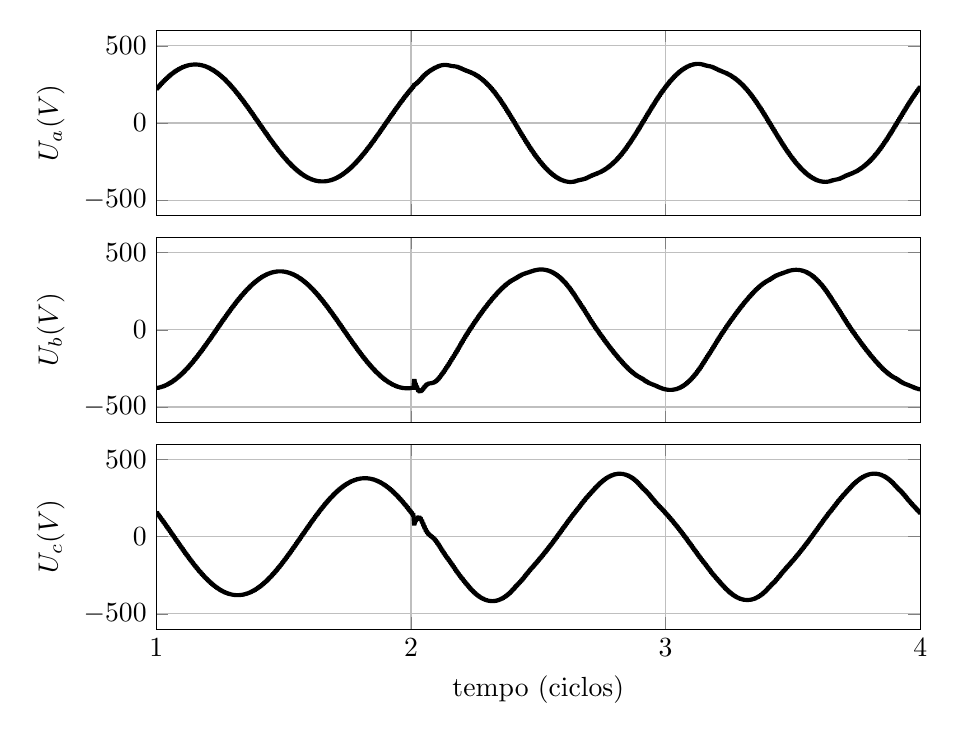
\begin{tikzpicture}

\begin{axis}[%
width=0.8\textwidth,
height=0.193917089240149\textwidth,
scale only axis,
xmin=0.316666666666667,
xmax=0.366666666666667,
xtick={0.316666666666667,0.333333333333333,0.35,0.366666666666667},
xticklabels={\empty},
xmajorgrids,
ymin=-600,
ymax=600,
ytick={-500,    0,  500},
ylabel={$\text{U}_\text{b}\text{ (V)}$},
ymajorgrids,
name=plot2,
scaled x ticks = false,
legend columns=-1,
legend style={/tikz/every even column/.append style={column sep=0.3cm}},
legend style={font=\footnotesize}
]
\addplot [color=black,solid,line width=1.5pt,forget plot]
  table[row sep=crcr]{0.316658333333333	-377.723085698266\\
0.3167	-376.586723778496\\
0.316741666666667	-376.586723778496\\
0.316783333333333	-375.078923942871\\
0.316825	-375.078923942871\\
0.316866666666667	-373.201183557557\\
0.316908333333333	-373.201183557557\\
0.31695	-370.955359679074\\
0.316991666666667	-370.955359679074\\
0.317033333333333	-368.343680965246\\
0.317075	-368.343680965246\\
0.317116666666667	-365.368751272189\\
0.317158333333333	-365.368751272189\\
0.3172	-362.033546182555\\
0.317241666666667	-362.033546182555\\
0.317283333333333	-358.341404810258\\
0.317325	-358.341404810258\\
0.317366666666667	-354.29601946274\\
0.317408333333333	-354.29601946274\\
0.31745	-349.901425336706\\
0.317491666666667	-349.901425336706\\
0.317533333333333	-345.161991678398\\
0.317575	-345.161991678398\\
0.317616666666667	-340.082415007475\\
0.317658333333333	-340.082415007475\\
0.3177	-334.667714301187\\
0.317741666666667	-334.667714301187\\
0.317783333333333	-328.923227572974\\
0.317825	-328.923227572974\\
0.317866666666667	-322.854609083496\\
0.317908333333333	-322.854609083496\\
0.31795	-316.467826451787\\
0.317991666666667	-316.467826451787\\
0.318033333333333	-309.769157112268\\
0.318075	-309.769157112268\\
0.318116666666667	-302.765183805345\\
0.318158333333333	-302.765183805345\\
0.3182	-295.462789021633\\
0.318241666666667	-295.462789021633\\
0.318283333333333	-287.869148495131\\
0.318325	-287.869148495131\\
0.318366666666667	-279.991723937524\\
0.318408333333333	-279.991723937524\\
0.31845	-271.838255227092\\
0.318491666666667	-271.838255227092\\
0.318533333333333	-263.416752229383\\
0.318575	-263.416752229383\\
0.318616666666667	-254.735486359231\\
0.318658333333333	-254.735486359231\\
0.3187	-245.802981925607\\
0.318741666666667	-245.802981925607\\
0.318783333333333	-236.6280072728\\
0.318825	-236.6280072728\\
0.318866666666667	-227.219565832749\\
0.318908333333333	-227.219565832749\\
0.31895	-217.586887717469\\
0.318991666666667	-217.586887717469\\
0.319033333333333	-207.739424484696\\
0.319075	-207.739424484696\\
0.319116666666667	-197.686870803904\\
0.319158333333333	-197.686870803904\\
0.3192	-187.439263486291\\
0.319241666666667	-187.439263486291\\
0.319283333333333	-177.007031372265\\
0.319325	-177.007031372265\\
0.319366666666667	-166.400723674948\\
0.319408333333333	-166.400723674948\\
0.31945	-155.6307199546\\
0.319491666666667	-155.6307199546\\
0.319533333333333	-144.707346263981\\
0.319575	-144.707346263981\\
0.319616666666667	-133.641094664328\\
0.319658333333333	-133.641094664328\\
0.3197	-122.442727673415\\
0.319741666666667	-122.442727673415\\
0.319783333333333	-111.123278734636\\
0.319825	-111.123278734636\\
0.319866666666667	-99.6940002360541\\
0.319908333333333	-99.6940002360541\\
0.31995	-88.1662967730299\\
0.319991666666667	-88.1662967730299\\
0.320033333333333	-76.5516646999388\\
0.320075	-76.5516646999388\\
0.320116666666667	-64.8616480040377\\
0.320158333333333	-64.8616480040377\\
0.3202	-53.1078129245748\\
0.320241666666667	-53.1078129245748\\
0.320283333333333	-41.3017386424485\\
0.320325	-41.3017386424485\\
0.320366666666667	-29.4550186053735\\
0.320408333333333	-29.4550186053735\\
0.32045	-17.5792663930844\\
0.320491666666667	-17.5792663930844\\
0.320533333333333	-5.68612092557823\\
0.320575	-5.68612092557823\\
0.320616666666667	6.2127524201114\\
0.320658333333333	6.2127524201114\\
0.3207	18.105666253858\\
0.320741666666667	18.105666253858\\
0.320783333333333	29.9809209740117\\
0.320825	29.9809209740117\\
0.320866666666667	41.8268186183045\\
0.320908333333333	41.8268186183045\\
0.32095	53.631678981668\\
0.320991666666667	53.631678981668\\
0.321033333333333	65.3838562807079\\
0.321075	65.3838562807079\\
0.321116666666667	77.0717550613194\\
0.321158333333333	77.0717550613194\\
0.3212	88.6838446142487\\
0.321241666666667	88.6838446142487\\
0.321283333333333	100.208671712027\\
0.321325	100.208671712027\\
0.321366666666667	111.6348719068\\
0.321408333333333	111.6348719068\\
0.32145	122.951179824381\\
0.321491666666667	122.951179824381\\
0.321533333333333	134.14643897231\\
0.321575	134.14643897231\\
0.321616666666667	145.209611528874\\
0.321658333333333	145.209611528874\\
0.3217	156.129788391287\\
0.321741666666667	156.129788391287\\
0.321783333333333	166.896199602751\\
0.321825	166.896199602751\\
0.321866666666667	177.498225133841\\
0.321908333333333	177.498225133841\\
0.32195	187.925405900222\\
0.321991666666667	187.925405900222\\
0.322033333333333	198.167454859908\\
0.322075	198.167454859908\\
0.322116666666667	208.214268041585\\
0.322158333333333	208.214268041585\\
0.3222	218.055935396159\\
0.322241666666667	218.055935396159\\
0.322283333333333	227.682751419264\\
0.322325	227.682751419264\\
0.322366666666667	237.085225549088\\
0.322408333333333	237.085225549088\\
0.32245	246.254092392214\\
0.322491666666667	246.254092392214\\
0.322533333333333	255.180321867299\\
0.322575	255.180321867299\\
0.322616666666667	263.855129383534\\
0.322658333333333	263.855129383534\\
0.3227	272.26998619054\\
0.322741666666667	272.26998619054\\
0.322783333333333	280.416630045836\\
0.322825	280.416630045836\\
0.322866666666667	288.287076317351\\
0.322908333333333	288.287076317351\\
0.32295	295.873629460527\\
0.322991666666667	295.873629460527\\
0.323033333333333	303.168894086837\\
0.323075	303.168894086837\\
0.323116666666667	310.165782141413\\
0.323158333333333	310.165782141413\\
0.3232	316.857502505702\\
0.323241666666667	316.857502505702\\
0.323283333333333	323.237410711189\\
0.323325	323.237410711189\\
0.323366666666667	329.298465304494\\
0.323408333333333	329.298465304494\\
0.32345	335.032940877286\\
0.323491666666667	335.032940877286\\
0.323533333333333	340.433778089715\\
0.323575	340.433778089715\\
0.323616666666667	345.496008515558\\
0.323658333333333	345.496008515558\\
0.3237	350.216089241188\\
0.323741666666667	350.216089241188\\
0.323783333333333	354.590714854285\\
0.323825	354.590714854285\\
0.323866666666667	358.616245271799\\
0.323908333333333	358.616245271799\\
0.32395	362.28867598875\\
0.323991666666667	362.28867598875\\
0.324033333333333	365.603866403093\\
0.324075	365.603866403093\\
0.324116666666667	368.557830105438\\
0.324158333333333	368.557830105438\\
0.3242	371.14698467744\\
0.324241666666667	371.14698467744\\
0.324283333333333	373.368315025462\\
0.324325	373.368315025462\\
0.324366666666667	375.219441072503\\
0.324408333333333	375.219441072503\\
0.32445	376.698604902272\\
0.324491666666667	376.698604902272\\
0.324533333333333	377.804605390594\\
0.324575	377.804605390594\\
0.324616666666667	378.536711049029\\
0.324658333333333	378.536711049029\\
0.3247	378.89457690205\\
0.324741666666667	378.89457690205\\
0.324783333333333	378.878182191864\\
0.324825	378.878182191864\\
0.324866666666667	378.487795835975\\
0.324908333333333	378.487795835975\\
0.32495	377.723968278227\\
0.324991666666667	377.723968278227\\
0.325033333333333	376.587542986259\\
0.325075	376.587542986259\\
0.325116666666667	375.079678623678\\
0.325158333333333	375.079678623678\\
0.3252	373.201873355773\\
0.325241666666667	373.201873355773\\
0.325283333333333	370.955984906448\\
0.325325	370.955984906448\\
0.325366666666667	368.34424285761\\
0.325408333333333	368.34424285761\\
0.32545	365.369252419982\\
0.325491666666667	365.369252419982\\
0.325533333333333	362.033990949537\\
0.325575	362.033990949537\\
0.325616666666667	358.341799615764\\
0.325658333333333	358.341799615764\\
0.3257	354.29637287251\\
0.325741666666667	354.29637287251\\
0.325783333333333	349.901747968484\\
0.325825	349.901747968484\\
0.325866666666667	345.162295969421\\
0.325908333333333	345.162295969421\\
0.32595	340.082714909794\\
0.325991666666667	340.082714909794\\
0.326033333333333	334.668024969912\\
0.326075	334.668024969912\\
0.326116666666667	328.923565098519\\
0.326158333333333	328.923565098519\\
0.3262	322.854990299289\\
0.326241666666667	322.854990299289\\
0.326283333333333	316.468268829063\\
0.326325	316.468268829063\\
0.326366666666667	309.769678739274\\
0.326408333333333	309.769678739274\\
0.32645	302.76580344002\\
0.326491666666667	302.76580344002\\
0.326533333333333	295.46352620612\\
0.326575	295.46352620612\\
0.326616666666667	287.870023724931\\
0.326658333333333	287.870023724931\\
0.3267	279.99275888678\\
0.326741666666667	279.99275888678\\
0.326783333333333	271.839473042268\\
0.326825	271.839473042268\\
0.326866666666667	263.418177915058\\
0.326908333333333	263.418177915058\\
0.32695	254.737147291355\\
0.326991666666667	254.737147291355\\
0.327033333333333	245.804908536742\\
0.327075	245.804908536742\\
0.327116666666667	236.630233953394\\
0.327158333333333	236.630233953394\\
0.3272	227.22213205341\\
0.327241666666667	227.22213205341\\
0.327283333333333	217.589839194205\\
0.327325	217.589839194205\\
0.327366666666667	207.742813476948\\
0.327408333333333	207.742813476948\\
0.32745	197.690748171958\\
0.327491666666667	197.690748171958\\
0.327533333333333	187.443640894198\\
0.327575	187.443640894198\\
0.327616666666667	177.011825362749\\
0.327658333333333	177.011825362749\\
0.3277	166.405770179614\\
0.327741666666667	166.405770179614\\
0.327783333333333	155.635868101642\\
0.327825	155.635868101642\\
0.327866666666667	144.712520179611\\
0.327908333333333	144.712520179611\\
0.32795	133.646292221512\\
0.327991666666667	133.646292221512\\
0.328033333333333	122.447986519211\\
0.328075	122.447986519211\\
0.328116666666667	111.128638130733\\
0.328158333333333	111.128638130733\\
0.3282	99.6994735093165\\
0.328241666666667	99.6994735093165\\
0.328283333333333	88.1718588306136\\
0.328325	88.1718588306136\\
0.328366666666667	76.5572531712875\\
0.328408333333333	76.5572531712875\\
0.32845	64.8671736797616\\
0.328491666666667	64.8671736797616\\
0.328533333333333	53.1131743732041\\
0.328575	53.1131743732041\\
0.328616666666667	41.3068365291399\\
0.328658333333333	41.3068365291399\\
0.3287	29.4597666782387\\
0.328741666666667	29.4597666782387\\
0.328783333333333	17.5835977645907\\
0.328825	17.5835977645907\\
0.328866666666667	5.68998972084417\\
0.328908333333333	5.68998972084417\\
0.32895	-6.20937299888088\\
0.328991666666667	-6.20937299888088\\
0.329033333333333	-18.1027879552077\\
0.329075	-18.1027879552077\\
0.329116666666667	-29.9785451472021\\
0.329158333333333	-29.9785451472021\\
0.3292	-41.8249403501677\\
0.329241666666667	-41.8249403501677\\
0.329283333333333	-53.6302900618585\\
0.329325	-53.6302900618585\\
0.329366666666667	-65.3829468063473\\
0.329408333333333	-65.3829468063473\\
0.32945	-77.0713138539921\\
0.329491666666667	-77.0713138539921\\
0.329533333333333	-88.6838588313381\\
0.329575	-88.6838588313381\\
0.329616666666667	-100.209126092659\\
0.329658333333333	-100.209126092659\\
0.3297	-111.635748034836\\
0.329741666666667	-111.635748034836\\
0.329783333333333	-122.952455666325\\
0.329825	-122.952455666325\\
0.329866666666667	-134.148088804689\\
0.329908333333333	-134.148088804689\\
0.32995	-145.211606244939\\
0.329991666666667	-145.211606244939\\
0.330033333333333	-156.132096092484\\
0.330075	-156.132096092484\\
0.330116666666667	-166.898786342177\\
0.330158333333333	-166.898786342177\\
0.3302	-177.501055680916\\
0.330241666666667	-177.501055680916\\
0.330283333333333	-187.928444425067\\
0.330325	-187.928444425067\\
0.330366666666667	-198.170665477564\\
0.330408333333333	-198.170665477564\\
0.33045	-208.21761519744\\
0.330491666666667	-208.21761519744\\
0.330533333333333	-218.059384105748\\
0.330575	-218.059384105748\\
0.330616666666667	-227.686267394042\\
0.330658333333333	-227.686267394042\\
0.3307	-237.088775244765\\
0.330741666666667	-237.088775244765\\
0.330783333333333	-246.257643010826\\
0.330825	-246.257643010826\\
0.330866666666667	-255.183841332313\\
0.330908333333333	-255.183841332313\\
0.33095	-263.858586293167\\
0.330991666666667	-263.858586293167\\
0.331033333333333	-272.273349741191\\
0.331075	-272.273349741191\\
0.331116666666667	-280.419869907006\\
0.331158333333333	-280.419869907006\\
0.3312	-288.29016243285\\
0.331241666666667	-288.29016243285\\
0.331283333333333	-295.876531750755\\
0.331325	-295.876531750755\\
0.331366666666667	-303.171582042784\\
0.331408333333333	-303.171582042784\\
0.33145	-310.168224372754\\
0.331491666666667	-310.168224372754\\
0.331533333333333	-316.859666586207\\
0.331575	-316.859666586207\\
0.331616666666667	-323.239266132863\\
0.331658333333333	-323.239266132863\\
0.3317	-329.299997905177\\
0.331741666666667	-329.299997905177\\
0.331783333333333	-335.034174516609\\
0.331825	-335.034174516609\\
0.331866666666667	-340.434769270671\\
0.331908333333333	-340.434769270671\\
0.33195	-345.496809702631\\
0.331991666666667	-345.496809702631\\
0.332033333333333	-350.216724523872\\
0.332075	-350.216724523872\\
0.332116666666667	-354.591180653519\\
0.332158333333333	-354.591180653519\\
0.3322	-358.616523838194\\
0.332241666666667	-358.616523838194\\
0.332283333333333	-362.288750228316\\
0.332325	-362.288750228316\\
0.332366666666667	-365.603730340961\\
0.332408333333333	-365.603730340961\\
0.33245	-368.557493442448\\
0.332491666666667	-368.557493442448\\
0.332533333333333	-371.146472117679\\
0.332575	-371.146472117679\\
0.332616666666667	-373.367662092301\\
0.332658333333333	-373.367662092301\\
0.3327	-375.218688387832\\
0.332741666666667	-375.218688387832\\
0.332783333333333	-376.697792634348\\
0.332825	-376.697792634348\\
0.332866666666667	-377.803769014554\\
0.332908333333333	-377.803769014554\\
0.33295	-378.535878926511\\
0.332991666666667	-378.535878926511\\
0.333033333333333	-378.893769636932\\
0.333075	-378.893769636932\\
0.333116666666667	-378.877413350589\\
0.333158333333333	-378.877413350589\\
0.3332	-378.487073457233\\
0.333241666666667	-378.487073457233\\
0.333283333333333	-377.723296609494\\
0.333325	-377.723296609494\\
0.333366666666667	-376.586924015447\\
0.333408333333333	-376.586924015447\\
0.33345	-375.079113157694\\
0.333491666666667	-375.079113157694\\
0.333533333333333	-331.053959173598\\
0.333575	-331.053959173598\\
0.333616666666667	-355.566522011512\\
0.333658333333333	-355.566522011512\\
0.3337	-373.445816485349\\
0.333741666666667	-373.445816485349\\
0.333783333333333	-390.060728449125\\
0.333825	-390.060728449125\\
0.333866666666667	-397.844659076646\\
0.333908333333333	-397.844659076646\\
0.33395	-397.607802023386\\
0.333991666666667	-397.607802023386\\
0.334033333333333	-391.060112093255\\
0.334075	-391.060112093255\\
0.334116666666667	-381.094479206499\\
0.334158333333333	-381.094479206499\\
0.3342	-370.432541041817\\
0.334241666666667	-370.432541041817\\
0.334283333333333	-361.10933181306\\
0.334325	-361.10933181306\\
0.334366666666667	-354.187694656387\\
0.334408333333333	-354.187694656387\\
0.33445	-349.799439727971\\
0.334491666666667	-349.799439727971\\
0.334533333333333	-347.372660995052\\
0.334575	-347.372660995052\\
0.334616666666667	-345.947097926559\\
0.334658333333333	-345.947097926559\\
0.3347	-344.482120632058\\
0.334741666666667	-344.482120632058\\
0.334783333333333	-342.09474327366\\
0.334825	-342.09474327366\\
0.334866666666667	-338.197725129126\\
0.334908333333333	-338.197725129126\\
0.33495	-332.537670597275\\
0.334991666666667	-332.537670597275\\
0.335033333333333	-325.15388006198\\
0.335075	-325.15388006198\\
0.335116666666667	-316.28916703799\\
0.335158333333333	-316.28916703799\\
0.3352	-306.284769550907\\
0.335241666666667	-306.284769550907\\
0.335283333333333	-295.485470833566\\
0.335325	-295.485470833566\\
0.335366666666667	-284.171376318267\\
0.335408333333333	-284.171376318267\\
0.33545	-272.522566002453\\
0.335491666666667	-272.522566002453\\
0.335533333333333	-260.61442814232\\
0.335575	-260.61442814232\\
0.335616666666667	-248.436427908707\\
0.335658333333333	-248.436427908707\\
0.3357	-235.926679683468\\
0.335741666666667	-235.926679683468\\
0.335783333333333	-223.037264128933\\
0.335825	-223.037264128933\\
0.335866666666667	-209.851831411951\\
0.335908333333333	-209.851831411951\\
0.33595	-196.611666331073\\
0.335991666666667	-196.611666331073\\
0.336033333333333	-183.476393437186\\
0.336075	-183.476393437186\\
0.336116666666667	-170.356767061117\\
0.336158333333333	-170.356767061117\\
0.3362	-157.055083569433\\
0.336241666666667	-157.055083569433\\
0.336283333333333	-143.429914658155\\
0.336325	-143.429914658155\\
0.336366666666667	-129.458136162372\\
0.336408333333333	-129.458136162372\\
0.33645	-115.222320815206\\
0.336491666666667	-115.222320815206\\
0.336533333333333	-100.866949128386\\
0.336575	-100.866949128386\\
0.336616666666667	-86.5509299822073\\
0.336658333333333	-86.5509299822073\\
0.3367	-72.41027026342\\
0.336741666666667	-72.41027026342\\
0.336783333333333	-58.5363796842563\\
0.336825	-58.5363796842563\\
0.336866666666667	-44.9700673537924\\
0.336908333333333	-44.9700673537924\\
0.33695	-31.707889473305\\
0.336991666666667	-31.707889473305\\
0.337033333333333	-18.7158965281947\\
0.337075	-18.7158965281947\\
0.337116666666667	-5.94573969853337\\
0.337158333333333	-5.94573969853337\\
0.3372	6.65091467907677\\
0.337241666666667	6.65091467907677\\
0.337283333333333	19.1121725057594\\
0.337325	19.1121725057594\\
0.337366666666667	31.4608004356482\\
0.337408333333333	31.4608004356482\\
0.33745	43.7037890472732\\
0.337491666666667	43.7037890472732\\
0.337533333333333	55.8353146508486\\
0.337575	55.8353146508486\\
0.337616666666667	67.8414871651914\\
0.337658333333333	67.8414871651914\\
0.3377	79.7053679758756\\
0.337741666666667	79.7053679758756\\
0.337783333333333	91.4111249732799\\
0.337825	91.4111249732799\\
0.337866666666667	102.946699116045\\
0.337908333333333	102.946699116045\\
0.33795	114.304846735082\\
0.337991666666667	114.304846735082\\
0.338033333333333	125.48279788958\\
0.338075	125.48279788958\\
0.338116666666667	136.480988520722\\
0.338158333333333	136.480988520722\\
0.3382	147.301382532013\\
0.338241666666667	147.301382532013\\
0.338283333333333	157.945834901859\\
0.338325	157.945834901859\\
0.338366666666667	168.414824976718\\
0.338408333333333	168.414824976718\\
0.33845	178.706689071158\\
0.338491666666667	178.706689071158\\
0.338533333333333	188.817360960719\\
0.338575	188.817360960719\\
0.338616666666667	198.740516451167\\
0.338658333333333	198.740516451167\\
0.3387	208.467965212707\\
0.338741666666667	208.467965212707\\
0.338783333333333	217.990125931066\\
0.338825	217.990125931066\\
0.338866666666667	227.296449162136\\
0.338908333333333	227.296449162136\\
0.33895	236.375699087072\\
0.338991666666667	236.375699087072\\
0.339033333333333	245.216055297035\\
0.339075	245.216055297035\\
0.339116666666667	253.805036957062\\
0.339158333333333	253.805036957062\\
0.3392	262.129277455222\\
0.339241666666667	262.129277455222\\
0.339283333333333	270.174186139085\\
0.339325	270.174186139085\\
0.339366666666667	277.923527251179\\
0.339408333333333	277.923527251179\\
0.33945	285.358930126453\\
0.339491666666667	285.358930126453\\
0.339533333333333	292.459328207278\\
0.339575	292.459328207278\\
0.339616666666667	299.200325675121\\
0.339658333333333	299.200325675121\\
0.3397	305.553558239489\\
0.339741666666667	305.553558239489\\
0.339783333333333	311.486405727299\\
0.339825	311.486405727299\\
0.339866666666667	316.963488313754\\
0.339908333333333	316.963488313754\\
0.33995	321.955622281295\\
0.339991666666667	321.955622281295\\
0.340033333333333	326.51038780251\\
0.340075	326.51038780251\\
0.340116666666667	330.894031493026\\
0.340158333333333	330.894031493026\\
0.3402	335.528606477071\\
0.340241666666667	335.528606477071\\
0.340283333333333	340.570364797468\\
0.340325	340.570364797468\\
0.340366666666667	345.770463847633\\
0.340408333333333	345.770463847633\\
0.34045	350.748908572128\\
0.340491666666667	350.748908572128\\
0.340533333333333	355.229203107812\\
0.340575	355.229203107812\\
0.340616666666667	359.114152112252\\
0.340658333333333	359.114152112252\\
0.3407	362.460955225898\\
0.340741666666667	362.460955225898\\
0.340783333333333	365.41785357704\\
0.340825	365.41785357704\\
0.340866666666667	368.157753621937\\
0.340908333333333	368.157753621937\\
0.34095	370.82624186103\\
0.340991666666667	370.82624186103\\
0.341033333333333	373.510998358136\\
0.341075	373.510998358136\\
0.341116666666667	376.232712187331\\
0.341158333333333	376.232712187331\\
0.3412	378.953067740294\\
0.341241666666667	378.953067740294\\
0.341283333333333	381.593124168933\\
0.341325	381.593124168933\\
0.341366666666667	384.055211723504\\
0.341408333333333	384.055211723504\\
0.34145	386.242756535565\\
0.341491666666667	386.242756535565\\
0.341533333333333	388.074514121078\\
0.341575	388.074514121078\\
0.341616666666667	389.4918829744\\
0.341658333333333	389.4918829744\\
0.3417	390.459793971863\\
0.341741666666667	390.459793971863\\
0.341783333333333	390.962859313687\\
0.341825	390.962859313687\\
0.341866666666667	390.998956997765\\
0.341908333333333	390.998956997765\\
0.34195	390.572324781683\\
0.341991666666667	390.572324781683\\
0.342033333333333	389.68773571272\\
0.342075	389.68773571272\\
0.342116666666667	388.346645879388\\
0.342158333333333	388.346645879388\\
0.3422	386.545537229963\\
0.342241666666667	386.545537229963\\
0.342283333333333	384.276158205878\\
0.342325	384.276158205878\\
0.342366666666667	381.527055310504\\
0.342408333333333	381.527055310504\\
0.34245	378.285700019777\\
0.342491666666667	378.285700019777\\
0.342533333333333	374.540592256173\\
0.342575	374.540592256173\\
0.342616666666667	370.282895838412\\
0.342658333333333	370.282895838412\\
0.3427	365.507390756861\\
0.342741666666667	365.507390756861\\
0.342783333333333	360.212725707634\\
0.342825	360.212725707634\\
0.342866666666667	354.401100495321\\
0.342908333333333	354.401100495321\\
0.34295	348.077584159459\\
0.342991666666667	348.077584159459\\
0.343033333333333	341.249285993621\\
0.343075	341.249285993621\\
0.343116666666667	333.924559113093\\
0.343158333333333	333.924559113093\\
0.3432	326.112351511447\\
0.343241666666667	326.112351511447\\
0.343283333333333	317.821748416951\\
0.343325	317.821748416951\\
0.343366666666667	309.061688184461\\
0.343408333333333	309.061688184461\\
0.34345	299.840791250307\\
0.343491666666667	299.840791250307\\
0.343533333333333	290.16722085235\\
0.343575	290.16722085235\\
0.343616666666667	280.048494368801\\
0.343658333333333	280.048494368801\\
0.3437	269.49118554204\\
0.343741666666667	269.49118554204\\
0.343783333333333	258.500513859365\\
0.343825	258.500513859365\\
0.343866666666667	247.079969056574\\
0.343908333333333	247.079969056574\\
0.34395	235.231596212627\\
0.343991666666667	235.231596212627\\
0.344033333333333	222.959248035688\\
0.344075	222.959248035688\\
0.344116666666667	210.294484360706\\
0.344158333333333	210.294484360706\\
0.3442	197.380821214263\\
0.344241666666667	197.380821214263\\
0.344283333333333	184.507370352904\\
0.344325	184.507370352904\\
0.344366666666667	171.894108559872\\
0.344408333333333	171.894108559872\\
0.34445	159.48943955546\\
0.344491666666667	159.48943955546\\
0.344533333333333	147.082800148723\\
0.344575	147.082800148723\\
0.344616666666667	134.48392975091\\
0.344658333333333	134.48392975091\\
0.3447	121.608197877001\\
0.344741666666667	121.608197877001\\
0.344783333333333	108.481692956559\\
0.344825	108.481692956559\\
0.344866666666667	95.2073277047852\\
0.344908333333333	95.2073277047852\\
0.34495	81.9206499726103\\
0.344991666666667	81.9206499726103\\
0.345033333333333	68.7509283943436\\
0.345075	68.7509283943436\\
0.345116666666667	55.7949153079795\\
0.345158333333333	55.7949153079795\\
0.3452	43.1051973184324\\
0.345241666666667	43.1051973184324\\
0.345283333333333	30.6913029919792\\
0.345325	30.6913029919792\\
0.345366666666667	18.5295910406299\\
0.345408333333333	18.5295910406299\\
0.34545	6.57727867560945\\
0.345491666666667	6.57727867560945\\
0.345533333333333	-5.21352892244916\\
0.345575	-5.21352892244916\\
0.345616666666667	-16.884732165864\\
0.345658333333333	-16.884732165864\\
0.3457	-28.4655123545339\\
0.345741666666667	-28.4655123545339\\
0.345783333333333	-39.9701087926515\\
0.345825	-39.9701087926515\\
0.345866666666667	-51.3992460624834\\
0.345908333333333	-51.3992460624834\\
0.34595	-62.7438487413975\\
0.345991666666667	-62.7438487413975\\
0.346033333333333	-73.9896017205765\\
0.346075	-73.9896017205765\\
0.346116666666667	-85.121157413393\\
0.346158333333333	-85.121157413393\\
0.3462	-96.1252122103461\\
0.346241666666667	-96.1252122103461\\
0.346283333333333	-106.992134481337\\
0.346325	-106.992134481337\\
0.346366666666667	-117.71621864397\\
0.346408333333333	-117.71621864397\\
0.34645	-128.294902750556\\
0.346491666666667	-128.294902750556\\
0.346533333333333	-138.727400956601\\
0.346575	-138.727400956601\\
0.346616666666667	-149.013197921609\\
0.346658333333333	-149.013197921609\\
0.3467	-159.150755168705\\
0.346741666666667	-159.150755168705\\
0.346783333333333	-169.136616907445\\
0.346825	-169.136616907445\\
0.346866666666667	-178.964978776181\\
0.346908333333333	-178.964978776181\\
0.34695	-188.627664096056\\
0.346991666666667	-188.627664096056\\
0.347033333333333	-198.114382623149\\
0.347075	-198.114382623149\\
0.347116666666667	-207.413121347082\\
0.347158333333333	-207.413121347082\\
0.3472	-216.510528801266\\
0.347241666666667	-216.510528801266\\
0.347283333333333	-225.392189426761\\
0.347325	-225.392189426761\\
0.347366666666667	-234.042728181155\\
0.347408333333333	-234.042728181155\\
0.34745	-242.445725371265\\
0.347491666666667	-242.445725371265\\
0.347533333333333	-250.583449409381\\
0.347575	-250.583449409381\\
0.347616666666667	-258.436427518641\\
0.347658333333333	-258.436427518641\\
0.3477	-265.982873061162\\
0.347741666666667	-265.982873061162\\
0.347783333333333	-273.197981095398\\
0.347825	-273.197981095398\\
0.347866666666667	-280.053111551403\\
0.347908333333333	-280.053111551403\\
0.34795	-286.514959521713\\
0.347991666666667	-286.514959521713\\
0.348033333333333	-292.545146969492\\
0.348075	-292.545146969492\\
0.348116666666667	-298.101899398808\\
0.348158333333333	-298.101899398808\\
0.3482	-303.150058989071\\
0.348241666666667	-303.150058989071\\
0.348283333333333	-307.741124565849\\
0.348325	-307.741124565849\\
0.348366666666667	-312.184494142668\\
0.348408333333333	-312.184494142668\\
0.34845	-316.993078269569\\
0.348491666666667	-316.993078269569\\
0.348533333333333	-322.386471176387\\
0.348575	-322.386471176387\\
0.348616666666667	-328.086904389457\\
0.348658333333333	-328.086904389457\\
0.3487	-333.634303962111\\
0.348741666666667	-333.634303962111\\
0.348783333333333	-338.681322343217\\
0.348825	-338.681322343217\\
0.348866666666667	-343.096845198308\\
0.348908333333333	-343.096845198308\\
0.34895	-346.94155652964\\
0.348991666666667	-346.94155652964\\
0.349033333333333	-350.39246515908\\
0.349075	-350.39246515908\\
0.349116666666667	-353.661520896268\\
0.349158333333333	-353.661520896268\\
0.3492	-356.930720798577\\
0.349241666666667	-356.930720798577\\
0.349283333333333	-360.312979455071\\
0.349325	-360.312979455071\\
0.349366666666667	-363.839388505294\\
0.349408333333333	-363.839388505294\\
0.34945	-367.467767573894\\
0.349491666666667	-367.467767573894\\
0.349533333333333	-371.104477750465\\
0.349575	-371.104477750465\\
0.349616666666667	-374.631068068148\\
0.349658333333333	-374.631068068148\\
0.3497	-377.928793486934\\
0.349741666666667	-377.928793486934\\
0.349783333333333	-380.896524488929\\
0.349825	-380.896524488929\\
0.349866666666667	-383.46025084714\\
0.349908333333333	-383.46025084714\\
0.34995	-385.574651555104\\
0.349991666666667	-385.574651555104\\
0.350033333333333	-387.218711197641\\
0.350075	-387.218711197641\\
0.350116666666667	-388.388020979728\\
0.350158333333333	-388.388020979728\\
0.3502	-389.086322412681\\
0.350241666666667	-389.086322412681\\
0.350283333333333	-389.318265056282\\
0.350325	-389.318265056282\\
0.350366666666667	-389.084525480898\\
0.350408333333333	-389.084525480898\\
0.35045	-388.379612290062\\
0.350491666666667	-388.379612290062\\
0.350533333333333	-387.192031057405\\
0.350575	-387.192031057405\\
0.350616666666667	-385.50608813227\\
0.350658333333333	-385.50608813227\\
0.3507	-383.304478923655\\
0.350741666666667	-383.304478923655\\
0.350783333333333	-380.57089349795\\
0.350825	-380.57089349795\\
0.350866666666667	-377.292089152202\\
0.350908333333333	-377.292089152202\\
0.35095	-373.459138569364\\
0.350991666666667	-373.459138569364\\
0.351033333333333	-369.067820550881\\
0.351075	-369.067820550881\\
0.351116666666667	-364.118301768284\\
0.351158333333333	-364.118301768284\\
0.3512	-358.614358042697\\
0.351241666666667	-358.614358042697\\
0.351283333333333	-352.562402718406\\
0.351325	-352.562402718406\\
0.351366666666667	-345.970547765741\\
0.351408333333333	-345.970547765741\\
0.35145	-338.847846274726\\
0.351491666666667	-338.847846274726\\
0.351533333333333	-331.203778757477\\
0.351575	-331.203778757477\\
0.351616666666667	-323.04797020633\\
0.351658333333333	-323.04797020633\\
0.3517	-314.39007205322\\
0.351741666666667	-314.39007205322\\
0.351783333333333	-305.239716754853\\
0.351825	-305.239716754853\\
0.351866666666667	-295.606450118041\\
0.351908333333333	-295.606450118041\\
0.35195	-285.499562206261\\
0.351991666666667	-285.499562206261\\
0.352033333333333	-274.927768645022\\
0.352075	-274.927768645022\\
0.352116666666667	-263.898750386451\\
0.352158333333333	-263.898750386451\\
0.3522	-252.418694924988\\
0.352241666666667	-252.418694924988\\
0.352283333333333	-240.492397886311\\
0.352325	-240.492397886311\\
0.352366666666667	-228.125947274508\\
0.352408333333333	-228.125947274508\\
0.35245	-215.348409104807\\
0.352491666666667	-215.348409104807\\
0.352533333333333	-202.289599450389\\
0.352575	-202.289599450389\\
0.352616666666667	-189.223743821868\\
0.352658333333333	-189.223743821868\\
0.3527	-176.379208719445\\
0.352741666666667	-176.379208719445\\
0.352783333333333	-163.726000022735\\
0.352825	-163.726000022735\\
0.352866666666667	-151.067803244203\\
0.352908333333333	-151.067803244203\\
0.35295	-138.218894529514\\
0.352991666666667	-138.218894529514\\
0.353033333333333	-125.092906412442\\
0.353075	-125.092906412442\\
0.353116666666667	-111.711266961333\\
0.353158333333333	-111.711266961333\\
0.3532	-98.1717617623561\\
0.353241666666667	-98.1717617623561\\
0.353283333333333	-84.606026368675\\
0.353325	-84.606026368675\\
0.353366666666667	-71.1415440461283\\
0.353408333333333	-71.1415440461283\\
0.35345	-57.8755976757111\\
0.353491666666667	-57.8755976757111\\
0.353533333333333	-44.8632491753258\\
0.353575	-44.8632491753258\\
0.353616666666667	-32.1177523558641\\
0.353658333333333	-32.1177523558641\\
0.3537	-19.6196605712489\\
0.353741666666667	-19.6196605712489\\
0.353783333333333	-7.33017611953616\\
0.353825	-7.33017611953616\\
0.353866666666667	4.79528596240854\\
0.353908333333333	4.79528596240854\\
0.35395	16.7962089615764\\
0.353991666666667	16.7962089615764\\
0.354033333333333	28.7002458702663\\
0.354075	28.7002458702663\\
0.354116666666667	40.5208361198962\\
0.354158333333333	40.5208361198962\\
0.3542	52.2583945768098\\
0.354241666666667	52.2583945768098\\
0.354283333333333	63.9037820451212\\
0.354325	63.9037820451212\\
0.354366666666667	75.4426677745932\\
0.354408333333333	75.4426677745932\\
0.35445	86.8596128178869\\
0.354491666666667	86.8596128178869\\
0.354533333333333	98.1411008420367\\
0.354575	98.1411008420367\\
0.354616666666667	109.277185521684\\
0.354658333333333	109.277185521684\\
0.3547	120.261806239716\\
0.354741666666667	120.261806239716\\
0.354783333333333	131.092084681737\\
0.354825	131.092084681737\\
0.354866666666667	141.767032559822\\
0.354908333333333	141.767032559822\\
0.35495	152.286104127589\\
0.354991666666667	152.286104127589\\
0.355033333333333	162.647935503272\\
0.355075	162.647935503272\\
0.355116666666667	172.849461167547\\
0.355158333333333	172.849461167547\\
0.3552	182.885476549861\\
0.355241666666667	182.885476549861\\
0.355283333333333	192.74859971663\\
0.355325	192.74859971663\\
0.355366666666667	202.429515642445\\
0.355408333333333	202.429515642445\\
0.35545	211.917359809411\\
0.355491666666667	211.917359809411\\
0.355533333333333	221.200107736149\\
0.355575	221.200107736149\\
0.355616666666667	230.264870122842\\
0.355658333333333	230.264870122842\\
0.3557	239.09803559447\\
0.355741666666667	239.09803559447\\
0.355783333333333	247.685242426249\\
0.355825	247.685242426249\\
0.355866666666667	256.01118897413\\
0.355908333333333	256.01118897413\\
0.35595	264.059306139522\\
0.355991666666667	264.059306139522\\
0.356033333333333	271.811314698462\\
0.356075	271.811314698462\\
0.356116666666667	279.246680549618\\
0.356158333333333	279.246680549618\\
0.3562	286.341972975943\\
0.356241666666667	286.341972975943\\
0.356283333333333	293.070152149675\\
0.356325	293.070152149675\\
0.356366666666667	299.399942608354\\
0.356408333333333	299.399942608354\\
0.35645	305.295957969326\\
0.356491666666667	305.295957969326\\
0.356533333333333	310.722117987443\\
0.356575	310.722117987443\\
0.356616666666667	315.666572995038\\
0.356658333333333	315.666572995038\\
0.3567	320.2542487815\\
0.356741666666667	320.2542487815\\
0.356783333333333	324.856446487095\\
0.356825	324.856446487095\\
0.356866666666667	329.852922874641\\
0.356908333333333	329.852922874641\\
0.35695	335.222065427616\\
0.356991666666667	335.222065427616\\
0.357033333333333	340.613534200536\\
0.357075	340.613534200536\\
0.357116666666667	345.656716837671\\
0.357158333333333	345.656716837671\\
0.3572	350.137311127185\\
0.357241666666667	350.137311127185\\
0.357283333333333	354.025303001667\\
0.357325	354.025303001667\\
0.357366666666667	357.426706873729\\
0.357408333333333	357.426706873729\\
0.35745	360.513281632962\\
0.357491666666667	360.513281632962\\
0.357533333333333	363.458209267499\\
0.357575	363.458209267499\\
0.357616666666667	366.390734543561\\
0.357658333333333	366.390734543561\\
0.3577	369.373754140581\\
0.357741666666667	369.373754140581\\
0.357783333333333	372.40226656797\\
0.357825	372.40226656797\\
0.357866666666667	375.416874434613\\
0.357908333333333	375.416874434613\\
0.35795	378.325110579895\\
0.357991666666667	378.325110579895\\
0.358033333333333	381.023855656326\\
0.358075	381.023855656326\\
0.358116666666667	383.417862668434\\
0.358158333333333	383.417862668434\\
0.3582	385.431672240814\\
0.358241666666667	385.431672240814\\
0.358283333333333	387.014368333221\\
0.358325	387.014368333221\\
0.358366666666667	388.138270008866\\
0.358408333333333	388.138270008866\\
0.35845	388.793592864896\\
0.358491666666667	388.793592864896\\
0.358533333333333	388.981356900916\\
0.358575	388.981356900916\\
0.358616666666667	388.706518452935\\
0.358658333333333	388.706518452935\\
0.3587	387.972682278112\\
0.358741666666667	387.972682278112\\
0.358783333333333	386.779028302941\\
0.358825	386.779028302941\\
0.358866666666667	385.119444190964\\
0.358908333333333	385.119444190964\\
0.35895	382.983399951863\\
0.358991666666667	382.983399951863\\
0.359033333333333	380.357871809701\\
0.359075	380.357871809701\\
0.359116666666667	377.229608324181\\
0.359158333333333	377.229608324181\\
0.3592	373.587164771571\\
0.359241666666667	373.587164771571\\
0.359283333333333	369.422335152074\\
0.359325	369.422335152074\\
0.359366666666667	364.730847206549\\
0.359408333333333	364.730847206549\\
0.35945	359.512371988876\\
0.359491666666667	359.512371988876\\
0.359533333333333	353.770022978723\\
0.359575	353.770022978723\\
0.359616666666667	347.509570477371\\
0.359658333333333	347.509570477371\\
0.3597	340.738586185096\\
0.359741666666667	340.738586185096\\
0.359783333333333	333.465680100964\\
0.359825	333.465680100964\\
0.359866666666667	325.699919967134\\
0.359908333333333	325.699919967134\\
0.35995	317.45045232578\\
0.359991666666667	317.45045232578\\
0.360033333333333	308.726287747113\\
0.360075	308.726287747113\\
0.360116666666667	299.536177702082\\
0.360158333333333	299.536177702082\\
0.3602	289.888497596475\\
0.360241666666667	289.888497596475\\
0.360283333333333	279.791057088036\\
0.360325	279.791057088036\\
0.360366666666667	269.250784501641\\
0.360408333333333	269.250784501641\\
0.36045	258.27329065012\\
0.360491666666667	258.27329065012\\
0.360533333333333	246.862472164031\\
0.360575	246.862472164031\\
0.360616666666667	235.020804269368\\
0.360658333333333	235.020804269368\\
0.3607	222.752710006781\\
0.360741666666667	222.752710006781\\
0.360783333333333	210.091801323474\\
0.360825	210.091801323474\\
0.360866666666667	197.185993975909\\
0.360908333333333	197.185993975909\\
0.36095	184.325618582163\\
0.360991666666667	184.325618582163\\
0.361033333333333	171.722625796759\\
0.361075	171.722625796759\\
0.361116666666667	159.316985749764\\
0.361158333333333	159.316985749764\\
0.3612	146.89655224484\\
0.361241666666667	146.89655224484\\
0.361283333333333	134.274769582802\\
0.361325	134.274769582802\\
0.361366666666667	121.372376006884\\
0.361408333333333	121.372376006884\\
0.36145	108.219776038739\\
0.361491666666667	108.219776038739\\
0.361533333333333	94.9220166008207\\
0.361575	94.9220166008207\\
0.361616666666667	81.614646304298\\
0.361658333333333	81.614646304298\\
0.3617	68.4254577689197\\
0.361741666666667	68.4254577689197\\
0.361783333333333	55.4490783962055\\
0.361825	55.4490783962055\\
0.361866666666667	42.7360509678476\\
0.361908333333333	42.7360509678476\\
0.36195	30.2944373262808\\
0.361991666666667	30.2944373262808\\
0.362033333333333	18.0999317872621\\
0.362075	18.0999317872621\\
0.362116666666667	6.10987697555117\\
0.362158333333333	6.10987697555117\\
0.3622	-5.72288379245039\\
0.362241666666667	-5.72288379245039\\
0.362283333333333	-17.4391559647083\\
0.362325	-17.4391559647083\\
0.362366666666667	-29.0669270842303\\
0.362408333333333	-29.0669270842303\\
0.36245	-40.6193498069394\\
0.362491666666667	-40.6193498069394\\
0.362533333333333	-52.0962957061184\\
0.362575	-52.0962957061184\\
0.362616666666667	-63.4881145894869\\
0.362658333333333	-63.4881145894869\\
0.3627	-74.7801727997866\\
0.362741666666667	-74.7801727997866\\
0.362783333333333	-85.95699646865\\
0.362825	-85.95699646865\\
0.362866666666667	-97.005268202752\\
0.362908333333333	-97.005268202752\\
0.36295	-107.915381191414\\
0.362991666666667	-107.915381191414\\
0.363033333333333	-118.68163930288\\
0.363075	-118.68163930288\\
0.363116666666667	-129.301446369291\\
0.363158333333333	-129.301446369291\\
0.3632	-139.77393479265\\
0.363241666666667	-139.77393479265\\
0.363283333333333	-150.09847450962\\
0.363325	-150.09847450962\\
0.363366666666667	-160.273404156851\\
0.363408333333333	-160.273404156851\\
0.36345	-170.295164440765\\
0.363491666666667	-170.295164440765\\
0.363533333333333	-180.157891159023\\
0.363575	-180.157891159023\\
0.363616666666667	-189.853409087089\\
0.363658333333333	-189.853409087089\\
0.3637	-199.371500840715\\
0.363741666666667	-199.371500840715\\
0.363783333333333	-208.700301424835\\
0.363825	-208.700301424835\\
0.363866666666667	-217.82668236852\\
0.363908333333333	-217.82668236852\\
0.36395	-226.736524925711\\
0.363991666666667	-226.736524925711\\
0.364033333333333	-235.414825364115\\
0.364075	-235.414825364115\\
0.364116666666667	-243.84561467942\\
0.364158333333333	-243.84561467942\\
0.3642	-252.011702190719\\
0.364241666666667	-252.011702190719\\
0.364283333333333	-259.894264193919\\
0.364325	-259.894264193919\\
0.364366666666667	-267.472296747565\\
0.364408333333333	-267.472296747565\\
0.36445	-274.721942890643\\
0.364491666666667	-274.721942890643\\
0.364533333333333	-281.615707001776\\
0.364575	-281.615707001776\\
0.364616666666667	-288.121631392846\\
0.364658333333333	-288.121631392846\\
0.3647	-294.202785652653\\
0.364741666666667	-294.202785652653\\
0.364783333333333	-299.818440515409\\
0.364825	-299.818440515409\\
0.364866666666667	-304.93209970605\\
0.364908333333333	-304.93209970605\\
0.36495	-309.575565237793\\
0.364991666666667	-309.575565237793\\
0.365033333333333	-314.012581745672\\
0.365075	-314.012581745672\\
0.365116666666667	-318.738236538347\\
0.365158333333333	-318.738236538347\\
0.3652	-324.025132661622\\
0.365241666666667	-324.025132661622\\
0.365283333333333	-329.648168153131\\
0.365325	-329.648168153131\\
0.365366666666667	-335.159687933284\\
0.365408333333333	-335.159687933284\\
0.36545	-340.199249987895\\
0.365491666666667	-340.199249987895\\
0.365533333333333	-344.614916167831\\
0.365575	-344.614916167831\\
0.365616666666667	-348.448453697907\\
0.365658333333333	-348.448453697907\\
0.3657	-351.863897978727\\
0.365741666666667	-351.863897978727\\
0.365783333333333	-355.067323932555\\
0.365825	-355.067323932555\\
0.365866666666667	-358.241309191347\\
0.365908333333333	-358.241309191347\\
0.36595	-361.504038503397\\
0.365991666666667	-361.504038503397\\
0.366033333333333	-364.894336620833\\
0.366075	-364.894336620833\\
0.366116666666667	-368.378119793744\\
0.366158333333333	-368.378119793744\\
0.3662	-371.868636134913\\
0.366241666666667	-371.868636134913\\
0.366283333333333	-375.252239474815\\
0.366325	-375.252239474815\\
0.366366666666667	-378.412712753345\\
0.366408333333333	-378.412712753345\\
0.36645	-381.249504392824\\
0.366491666666667	-381.249504392824\\
0.366533333333333	-383.687860969564\\
0.366575	-383.687860969564\\
0.366616666666667	-385.681109833679\\
0.366658333333333	-385.681109833679\\
};
\end{axis}

\begin{axis}[%
width=0.8\textwidth,
height=0.193917089240149\textwidth,
scale only axis,
xmin=0.316666666666667,
xmax=0.366666666666667,
xtick={0.316666666666667,0.333333333333333,0.35,0.366666666666667},
xticklabels={{1},{2},{3},{4}},
xlabel={tempo (ciclos)},
xmajorgrids,
ymin=-600,
ymax=600,
ytick={-500,    0,  500},
ylabel={$\text{U}_\text{c}\text{ (V)}$},
ymajorgrids,
at=(plot2.below south west),
anchor=above north west,
scaled x ticks = false,
legend columns=-1,
legend style={/tikz/every even column/.append style={column sep=0.3cm}},
legend style={font=\footnotesize}
]
\addplot [color=black,solid,line width=1.5pt,forget plot]
  table[row sep=crcr]{0.316658333333333	162.970553693369\\
0.3167	152.134366652308\\
0.316741666666667	152.134366652308\\
0.316783333333333	141.14831005675\\
0.316825	141.14831005675\\
0.316866666666667	130.023235612171\\
0.316908333333333	130.023235612171\\
0.31695	118.770126781016\\
0.316991666666667	118.770126781016\\
0.317033333333333	107.400101722771\\
0.317075	107.400101722771\\
0.317116666666667	95.9244081552081\\
0.317158333333333	95.9244081552081\\
0.3172	84.3544113952257\\
0.317241666666667	84.3544113952257\\
0.317283333333333	72.701577924984\\
0.317325	72.701577924984\\
0.317366666666667	60.9774570729016\\
0.317408333333333	60.9774570729016\\
0.31745	49.1936630040597\\
0.317491666666667	49.1936630040597\\
0.317533333333333	37.3618584558936\\
0.317575	37.3618584558936\\
0.317616666666667	25.4937408270424\\
0.317658333333333	25.4937408270424\\
0.3177	13.6010305245207\\
0.317741666666667	13.6010305245207\\
0.317783333333333	1.69546101270924\\
0.317825	1.69546101270924\\
0.317866666666667	-10.2112301875565\\
0.317908333333333	-10.2112301875565\\
0.31795	-22.1073102710107\\
0.317991666666667	-22.1073102710107\\
0.318033333333333	-33.9810602324472\\
0.318075	-33.9810602324472\\
0.318116666666667	-45.8207845611742\\
0.318158333333333	-45.8207845611742\\
0.3182	-57.6148216075114\\
0.318241666666667	-57.6148216075114\\
0.318283333333333	-69.3515545038083\\
0.318325	-69.3515545038083\\
0.318366666666667	-81.0194224196816\\
0.318408333333333	-81.0194224196816\\
0.31845	-92.6069319017156\\
0.318491666666667	-92.6069319017156\\
0.318533333333333	-104.102668074645\\
0.318575	-104.102668074645\\
0.318616666666667	-115.495305540439\\
0.318658333333333	-115.495305540439\\
0.3187	-126.773618886739\\
0.318741666666667	-126.773618886739\\
0.318783333333333	-137.926492811092\\
0.318825	-137.926492811092\\
0.318866666666667	-148.942932050852\\
0.318908333333333	-148.942932050852\\
0.31895	-159.812071858709\\
0.318991666666667	-159.812071858709\\
0.319033333333333	-170.5231917644\\
0.319075	-170.5231917644\\
0.319116666666667	-181.06575642652\\
0.319158333333333	-181.06575642652\\
0.3192	-191.42953407303\\
0.319241666666667	-191.42953407303\\
0.319283333333333	-201.604666016903\\
0.319325	-201.604666016903\\
0.319366666666667	-211.581414807252\\
0.319408333333333	-211.581414807252\\
0.31945	-221.34989413342\\
0.319491666666667	-221.34989413342\\
0.319533333333333	-230.900204960054\\
0.319575	-230.900204960054\\
0.319616666666667	-240.222675034997\\
0.319658333333333	-240.222675034997\\
0.3197	-249.307983285081\\
0.319741666666667	-249.307983285081\\
0.319783333333333	-258.147180154562\\
0.319825	-258.147180154562\\
0.319866666666667	-266.731655392224\\
0.319908333333333	-266.731655392224\\
0.31995	-275.053090965318\\
0.319991666666667	-275.053090965318\\
0.320033333333333	-283.103420134525\\
0.320075	-283.103420134525\\
0.320116666666667	-290.874802711353\\
0.320158333333333	-290.874802711353\\
0.3202	-298.359618907919\\
0.320241666666667	-298.359618907919\\
0.320283333333333	-305.550479087533\\
0.320325	-305.550479087533\\
0.320366666666667	-312.440243961342\\
0.320408333333333	-312.440243961342\\
0.32045	-319.022049113252\\
0.320491666666667	-319.022049113252\\
0.320533333333333	-325.289328632728\\
0.320575	-325.289328632728\\
0.320616666666667	-331.235834397501\\
0.320658333333333	-331.235834397501\\
0.3207	-336.855649514461\\
0.320741666666667	-336.855649514461\\
0.320783333333333	-342.143196100745\\
0.320825	-342.143196100745\\
0.320866666666667	-347.093238694001\\
0.320908333333333	-347.093238694001\\
0.32095	-351.700885056722\\
0.320991666666667	-351.700885056722\\
0.321033333333333	-355.961586078382\\
0.321075	-355.961586078382\\
0.321116666666667	-359.871136064135\\
0.321158333333333	-359.871136064135\\
0.3212	-363.425674130623\\
0.321241666666667	-363.425674130623\\
0.321283333333333	-366.621686882158\\
0.321325	-366.621686882158\\
0.321366666666667	-369.456012137793\\
0.321408333333333	-369.456012137793\\
0.32145	-371.925843211841\\
0.321491666666667	-371.925843211841\\
0.321533333333333	-374.028733221122\\
0.321575	-374.028733221122\\
0.321616666666667	-375.762598995818\\
0.321658333333333	-375.762598995818\\
0.3217	-377.125724285815\\
0.321741666666667	-377.125724285815\\
0.321783333333333	-378.116762135567\\
0.321825	-378.116762135567\\
0.321866666666667	-378.734736446567\\
0.321908333333333	-378.734736446567\\
0.32195	-378.979042846209\\
0.321991666666667	-378.979042846209\\
0.322033333333333	-378.849449026762\\
0.322075	-378.849449026762\\
0.322116666666667	-378.346094717328\\
0.322158333333333	-378.346094717328\\
0.3222	-377.469491420695\\
0.322241666666667	-377.469491420695\\
0.322283333333333	-376.220522004144\\
0.322325	-376.220522004144\\
0.322366666666667	-374.600440193894\\
0.322408333333333	-374.600440193894\\
0.32245	-372.61086999843\\
0.322491666666667	-372.61086999843\\
0.322533333333333	-370.253805081463\\
0.322575	-370.253805081463\\
0.322616666666667	-367.531608121488\\
0.322658333333333	-367.531608121488\\
0.3227	-364.447010227436\\
0.322741666666667	-364.447010227436\\
0.322783333333333	-361.00311051502\\
0.322825	-361.00311051502\\
0.322866666666667	-357.2033759492\\
0.322908333333333	-357.2033759492\\
0.32295	-353.051641405706\\
0.322991666666667	-353.051641405706\\
0.323033333333333	-348.55210919846\\
0.323075	-348.55210919846\\
0.323116666666667	-343.709344628697\\
0.323158333333333	-343.709344628697\\
0.3232	-338.52825390877\\
0.323241666666667	-338.52825390877\\
0.323283333333333	-333.013922177807\\
0.323325	-333.013922177807\\
0.323366666666667	-327.171058172122\\
0.323408333333333	-327.171058172122\\
0.32345	-321.003695577926\\
0.323491666666667	-321.003695577926\\
0.323533333333333	-314.516531402583\\
0.323575	-314.516531402583\\
0.323616666666667	-307.716339196424\\
0.323658333333333	-307.716339196424\\
0.3237	-300.611292060023\\
0.323741666666667	-300.611292060023\\
0.323783333333333	-293.209763076321\\
0.323825	-293.209763076321\\
0.323866666666667	-285.519741623125\\
0.323908333333333	-285.519741623125\\
0.32395	-277.54879215579\\
0.323991666666667	-277.54879215579\\
0.324033333333333	-269.304271125924\\
0.324075	-269.304271125924\\
0.324116666666667	-260.79360593688\\
0.324158333333333	-260.79360593688\\
0.3242	-252.02453349254\\
0.324241666666667	-252.02453349254\\
0.324283333333333	-243.005252378576\\
0.324325	-243.005252378576\\
0.324366666666667	-233.744479511389\\
0.324408333333333	-233.744479511389\\
0.32445	-224.251426359643\\
0.324491666666667	-224.251426359643\\
0.324533333333333	-214.535722784241\\
0.324575	-214.535722784241\\
0.324616666666667	-204.607319231369\\
0.324658333333333	-204.607319231369\\
0.3247	-194.476393109332\\
0.324741666666667	-194.476393109332\\
0.324783333333333	-184.153276152493\\
0.324825	-184.153276152493\\
0.324866666666667	-173.648409706627\\
0.324908333333333	-173.648409706627\\
0.32495	-162.972326585662\\
0.324991666666667	-162.972326585662\\
0.325033333333333	-152.135652762133\\
0.325075	-152.135652762133\\
0.325116666666667	-141.149119929114\\
0.325158333333333	-141.149119929114\\
0.3252	-130.023580401982\\
0.325241666666667	-130.023580401982\\
0.325283333333333	-118.770017987052\\
0.325325	-118.770017987052\\
0.325366666666667	-107.399551317653\\
0.325408333333333	-107.399551317653\\
0.32545	-95.9234288957582\\
0.325491666666667	-95.9234288957582\\
0.325533333333333	-84.3530171259215\\
0.325575	-84.3530171259215\\
0.325616666666667	-72.6997837486583\\
0.325658333333333	-72.6997837486583\\
0.3257	-60.9752793324054\\
0.325741666666667	-60.9752793324054\\
0.325783333333333	-49.1911190787728\\
0.325825	-49.1911190787728\\
0.325866666666667	-37.3589664176652\\
0.325908333333333	-37.3589664176652\\
0.32595	-25.4905190184515\\
0.325991666666667	-25.4905190184515\\
0.326033333333333	-13.5974971207829\\
0.326075	-13.5974971207829\\
0.326116666666667	-1.69163361404229\\
0.326158333333333	-1.69163361404229\\
0.3262	10.2153349073519\\
0.326241666666667	10.2153349073519\\
0.326283333333333	22.1116768548334\\
0.326325	22.1116768548334\\
0.326366666666667	33.9856746806564\\
0.326408333333333	33.9856746806564\\
0.32645	45.8256345451254\\
0.326491666666667	45.8256345451254\\
0.326533333333333	57.619896682525\\
0.326575	57.619896682525\\
0.326616666666667	69.356846348781\\
0.326658333333333	69.356846348781\\
0.3267	81.0249251286878\\
0.326741666666667	81.0249251286878\\
0.326783333333333	92.6126423517755\\
0.326825	92.6126423517755\\
0.326866666666667	104.108586394839\\
0.326908333333333	104.108586394839\\
0.32695	115.501435711804\\
0.326991666666667	115.501435711804\\
0.327033333333333	126.779969508188\\
0.327075	126.779969508188\\
0.327116666666667	137.933078066121\\
0.327158333333333	137.933078066121\\
0.3272	148.949772873188\\
0.327241666666667	148.949772873188\\
0.327283333333333	159.819197115413\\
0.327325	159.819197115413\\
0.327366666666667	170.530638546332\\
0.327408333333333	170.530638546332\\
0.32745	181.073562075667\\
0.327491666666667	181.073562075667\\
0.327533333333333	191.437698337058\\
0.327575	191.437698337058\\
0.327616666666667	201.613095062515\\
0.327658333333333	201.613095062515\\
0.3277	211.589935660001\\
0.327741666666667	211.589935660001\\
0.327783333333333	221.358348409748\\
0.327825	221.358348409748\\
0.327866666666667	230.908510590095\\
0.327908333333333	230.908510590095\\
0.32795	240.230824931129\\
0.327991666666667	240.230824931129\\
0.328033333333333	249.316011288028\\
0.328075	249.316011288028\\
0.328116666666667	258.155122791836\\
0.328158333333333	258.155122791836\\
0.3282	266.739524245654\\
0.328241666666667	266.739524245654\\
0.328283333333333	275.0608601025\\
0.328325	275.0608601025\\
0.328366666666667	283.111027166579\\
0.328408333333333	283.111027166579\\
0.32845	290.882159147744\\
0.328491666666667	290.882159147744\\
0.328533333333333	298.366624689893\\
0.328575	298.366624689893\\
0.328616666666667	305.557036824969\\
0.328658333333333	305.557036824969\\
0.3287	312.44626983943\\
0.328741666666667	312.44626983943\\
0.328783333333333	319.027479097028\\
0.328825	319.027479097028\\
0.328866666666667	325.294120041746\\
0.328908333333333	325.294120041746\\
0.32895	331.239963900123\\
0.328991666666667	331.239963900123\\
0.329033333333333	336.859109033448\\
0.329075	336.859109033448\\
0.329116666666667	342.145988100331\\
0.329158333333333	342.145988100331\\
0.3292	347.09537198353\\
0.329241666666667	347.09537198353\\
0.329283333333333	351.702371769095\\
0.329325	351.702371769095\\
0.329366666666667	355.96244001224\\
0.329408333333333	355.96244001224\\
0.32945	359.871372216336\\
0.329491666666667	359.871372216336\\
0.329533333333333	363.425309036832\\
0.329575	363.425309036832\\
0.329616666666667	366.620739324895\\
0.329658333333333	366.620739324895\\
0.3297	369.454503838896\\
0.329741666666667	369.454503838896\\
0.329783333333333	371.923799251079\\
0.329825	371.923799251079\\
0.329866666666667	374.026182065952\\
0.329908333333333	374.026182065952\\
0.32995	375.759572151591\\
0.329991666666667	375.759572151591\\
0.330033333333333	377.122255660091\\
0.330075	377.122255660091\\
0.330116666666667	378.112887248098\\
0.330158333333333	378.112887248098\\
0.3302	378.730491614484\\
0.330241666666667	378.730491614484\\
0.330283333333333	378.974464444218\\
0.330325	378.974464444218\\
0.330366666666667	378.844572880123\\
0.330408333333333	378.844572880123\\
0.33045	378.340955643699\\
0.330491666666667	378.340955643699\\
0.330533333333333	377.464122904322\\
0.330575	377.464122904322\\
0.330616666666667	376.214955966436\\
0.330658333333333	376.214955966436\\
0.3307	374.5947068181\\
0.330741666666667	374.5947068181\\
0.330783333333333	372.604997569562\\
0.330825	372.604997569562\\
0.330866666666667	370.24781981178\\
0.330908333333333	370.24781981178\\
0.33095	367.525533942416\\
0.330991666666667	367.525533942416\\
0.331033333333333	364.440868536929\\
0.331075	364.440868536929\\
0.331116666666667	360.996919873773\\
0.331158333333333	360.996919873773\\
0.3312	357.197151719323\\
0.331241666666667	357.197151719323\\
0.331283333333333	353.045395325139\\
0.331325	353.045395325139\\
0.331366666666667	348.545848895653\\
0.331408333333333	348.545848895653\\
0.33145	343.703073146214\\
0.331491666666667	343.703073146214\\
0.331533333333333	338.521969578445\\
0.331575	338.521969578445\\
0.331616666666667	333.00762165269\\
0.331658333333333	333.00762165269\\
0.3317	327.164750970432\\
0.331741666666667	327.164750970432\\
0.331783333333333	320.997425903535\\
0.331825	320.997425903535\\
0.331866666666667	314.51037292983\\
0.331908333333333	314.51037292983\\
0.33195	307.710358562834\\
0.331991666666667	307.710358562834\\
0.332033333333333	300.605524710562\\
0.332075	300.605524710562\\
0.332116666666667	293.204214153872\\
0.332158333333333	293.204214153872\\
0.3322	285.514399652687\\
0.332241666666667	285.514399652687\\
0.332283333333333	277.543644057549\\
0.332325	277.543644057549\\
0.332366666666667	269.299312867494\\
0.332408333333333	269.299312867494\\
0.33245	260.788847279147\\
0.332491666666667	260.788847279147\\
0.332533333333333	252.019997506399\\
0.332575	252.019997506399\\
0.332616666666667	243.000971448902\\
0.332658333333333	243.000971448902\\
0.3327	233.740489801388\\
0.332741666666667	233.740489801388\\
0.332783333333333	224.24776243952\\
0.332825	224.24776243952\\
0.332866666666667	214.532413566654\\
0.332908333333333	214.532413566654\\
0.33295	204.604385718927\\
0.332991666666667	204.604385718927\\
0.333033333333333	194.47384791024\\
0.333075	194.47384791024\\
0.333116666666667	184.151124352293\\
0.333158333333333	184.151124352293\\
0.3332	173.646650520602\\
0.333241666666667	173.646650520602\\
0.333283333333333	162.970955229482\\
0.333325	162.970955229482\\
0.333366666666667	152.134662109327\\
0.333408333333333	152.134662109327\\
0.33345	141.148501707592\\
0.333491666666667	141.148501707592\\
0.333533333333333	85.2185958814851\\
0.333575	85.2185958814851\\
0.333616666666667	103.85358356803\\
0.333658333333333	103.85358356803\\
0.3337	114.800275875281\\
0.333741666666667	114.800275875281\\
0.333783333333333	123.975397007369\\
0.333825	123.975397007369\\
0.333866666666667	123.377943898172\\
0.333908333333333	123.377943898172\\
0.33395	114.185678788677\\
0.333991666666667	114.185678788677\\
0.334033333333333	98.5111419960005\\
0.334075	98.5111419960005\\
0.334116666666667	79.6628198300563\\
0.334158333333333	79.6628198300563\\
0.3342	60.6620211608378\\
0.334241666666667	60.6620211608378\\
0.334283333333333	43.7012745349893\\
0.334325	43.7012745349893\\
0.334366666666667	29.8661132784312\\
0.334408333333333	29.8661132784312\\
0.33445	19.2141732193439\\
0.334491666666667	19.2141732193439\\
0.334533333333333	11.0503494515357\\
0.334575	11.0503494515357\\
0.334616666666667	4.28710409346159\\
0.334658333333333	4.28710409346159\\
0.3347	-2.21450610678728\\
0.334741666666667	-2.21450610678728\\
0.334783333333333	-9.38920504734886\\
0.334825	-9.38920504734886\\
0.334866666666667	-17.8264836303797\\
0.334908333333333	-17.8264836303797\\
0.33495	-27.7406545732471\\
0.334991666666667	-27.7406545732471\\
0.335033333333333	-39.0263220174088\\
0.335075	-39.0263220174088\\
0.335116666666667	-51.3632591548139\\
0.335158333333333	-51.3632591548139\\
0.3352	-64.3348409382022\\
0.335241666666667	-64.3348409382022\\
0.335283333333333	-77.5317160673345\\
0.335325	-77.5317160673345\\
0.335366666666667	-90.6236216733833\\
0.335408333333333	-90.6236216733833\\
0.33545	-103.393780349962\\
0.335491666666667	-103.393780349962\\
0.335533333333333	-115.739792932798\\
0.335575	-115.739792932798\\
0.335616666666667	-127.651329322379\\
0.335658333333333	-127.651329322379\\
0.3357	-139.179040798263\\
0.335741666666667	-139.179040798263\\
0.335783333333333	-150.430344961277\\
0.335825	-150.430344961277\\
0.335866666666667	-161.629114937787\\
0.335908333333333	-161.629114937787\\
0.33595	-173.1040447074\\
0.335991666666667	-173.1040447074\\
0.336033333333333	-185.033802537725\\
0.336075	-185.033802537725\\
0.336116666666667	-197.283225761293\\
0.336158333333333	-197.283225761293\\
0.3362	-209.559922755223\\
0.336241666666667	-209.559922755223\\
0.336283333333333	-221.600965697189\\
0.336325	-221.600965697189\\
0.336366666666667	-233.256478740937\\
0.336408333333333	-233.256478740937\\
0.33645	-244.493889991113\\
0.336491666666667	-244.493889991113\\
0.336533333333333	-255.364213064309\\
0.336575	-255.364213064309\\
0.336616666666667	-265.957760494535\\
0.336658333333333	-265.957760494535\\
0.3367	-276.364475872641\\
0.336741666666667	-276.364475872641\\
0.336783333333333	-286.646460849308\\
0.336825	-286.646460849308\\
0.336866666666667	-296.82494064566\\
0.336908333333333	-296.82494064566\\
0.33695	-306.880133797929\\
0.336991666666667	-306.880133797929\\
0.337033333333333	-316.760239490873\\
0.337075	-316.760239490873\\
0.337116666666667	-326.394972791455\\
0.337158333333333	-326.394972791455\\
0.3372	-335.709477976686\\
0.337241666666667	-335.709477976686\\
0.337283333333333	-344.635597931895\\
0.337325	-344.635597931895\\
0.337366666666667	-353.118914526971\\
0.337408333333333	-353.118914526971\\
0.33745	-361.12131852119\\
0.337491666666667	-361.12131852119\\
0.337533333333333	-368.619867292642\\
0.337575	-368.619867292642\\
0.337616666666667	-375.603238412026\\
0.337658333333333	-375.603238412026\\
0.3377	-382.067204667217\\
0.337741666666667	-382.067204667217\\
0.337783333333333	-388.010343565664\\
0.337825	-388.010343565664\\
0.337866666666667	-393.430792055182\\
0.337908333333333	-393.430792055182\\
0.33795	-398.324403907572\\
0.337991666666667	-398.324403907572\\
0.338033333333333	-402.684271681203\\
0.338075	-402.684271681203\\
0.338116666666667	-406.501302508889\\
0.338158333333333	-406.501302508889\\
0.3382	-409.765406448651\\
0.338241666666667	-409.765406448651\\
0.338283333333333	-412.466855046899\\
0.338325	-412.466855046899\\
0.338366666666667	-414.597475935023\\
0.338408333333333	-414.597475935023\\
0.33845	-416.151449744806\\
0.338491666666667	-416.151449744806\\
0.338533333333333	-417.125643398935\\
0.338575	-417.125643398935\\
0.338616666666667	-417.519521533044\\
0.338658333333333	-417.519521533044\\
0.3387	-417.334751057628\\
0.338741666666667	-417.334751057628\\
0.338783333333333	-416.574640324386\\
0.338825	-416.574640324386\\
0.338866666666667	-415.243543636688\\
0.338908333333333	-415.243543636688\\
0.33895	-413.346326137345\\
0.338991666666667	-413.346326137345\\
0.339033333333333	-410.88793775112\\
0.339075	-410.88793775112\\
0.339116666666667	-407.873099917022\\
0.339158333333333	-407.873099917022\\
0.3392	-404.306073419944\\
0.339241666666667	-404.306073419944\\
0.339283333333333	-400.190453297818\\
0.339325	-400.190453297818\\
0.339366666666667	-395.528927373469\\
0.339408333333333	-395.528927373469\\
0.33945	-390.322936359708\\
0.339491666666667	-390.322936359708\\
0.339533333333333	-384.572185275442\\
0.339575	-384.572185275442\\
0.339616666666667	-378.273987294707\\
0.339658333333333	-378.273987294707\\
0.3397	-371.422514107589\\
0.339741666666667	-371.422514107589\\
0.339783333333333	-364.008334480398\\
0.339825	-364.008334480398\\
0.339866666666667	-356.019703807512\\
0.339908333333333	-356.019703807512\\
0.33995	-347.451310152554\\
0.339991666666667	-347.451310152554\\
0.340033333333333	-338.374651955256\\
0.340075	-338.374651955256\\
0.340116666666667	-329.079783349174\\
0.340158333333333	-329.079783349174\\
0.3402	-320.012333679261\\
0.340241666666667	-320.012333679261\\
0.340283333333333	-311.351812548638\\
0.340325	-311.351812548638\\
0.340366666666667	-302.872254140232\\
0.340408333333333	-302.872254140232\\
0.34045	-294.216113166378\\
0.340491666666667	-294.216113166378\\
0.340533333333333	-285.12887765367\\
0.340575	-285.12887765367\\
0.340616666666667	-275.534832762294\\
0.340658333333333	-275.534832762294\\
0.3407	-265.512116000138\\
0.340741666666667	-265.512116000138\\
0.340783333333333	-255.2293223772\\
0.340825	-255.2293223772\\
0.340866666666667	-244.879086410513\\
0.340908333333333	-244.879086410513\\
0.34095	-234.626057174045\\
0.340991666666667	-234.626057174045\\
0.341033333333333	-224.576277116838\\
0.341075	-224.576277116838\\
0.341116666666667	-214.768070042425\\
0.341158333333333	-214.768070042425\\
0.3412	-205.180008548952\\
0.341241666666667	-205.180008548952\\
0.341283333333333	-195.749283586029\\
0.341325	-195.749283586029\\
0.341366666666667	-186.393599424394\\
0.341408333333333	-186.393599424394\\
0.34145	-177.031004550466\\
0.341491666666667	-177.031004550466\\
0.341533333333333	-167.59413746201\\
0.341575	-167.59413746201\\
0.341616666666667	-158.037557452057\\
0.341658333333333	-158.037557452057\\
0.3417	-148.338655028979\\
0.341741666666667	-148.338655028979\\
0.341783333333333	-138.49382494683\\
0.341825	-138.49382494683\\
0.341866666666667	-128.512077417217\\
0.341908333333333	-128.512077417217\\
0.34195	-118.408161324706\\
0.341991666666667	-118.408161324706\\
0.342033333333333	-108.196771602312\\
0.342075	-108.196771602312\\
0.342116666666667	-97.8887316295639\\
0.342158333333333	-97.8887316295639\\
0.3422	-87.4893737797058\\
0.342241666666667	-87.4893737797058\\
0.342283333333333	-76.9988211885817\\
0.342325	-76.9988211885817\\
0.342366666666667	-66.4135678196744\\
0.342408333333333	-66.4135678196744\\
0.34245	-55.7286553986473\\
0.342491666666667	-55.7286553986473\\
0.342533333333333	-44.9398244539784\\
0.342575	-44.9398244539784\\
0.342616666666667	-34.0452091212057\\
0.342658333333333	-34.0452091212057\\
0.3427	-23.0463567597564\\
0.342741666666667	-23.0463567597564\\
0.342783333333333	-11.9485574355951\\
0.342825	-11.9485574355951\\
0.342866666666667	-0.760614590325387\\
0.342908333333333	-0.760614590325387\\
0.34295	10.5057340271045\\
0.342991666666667	10.5057340271045\\
0.343033333333333	21.8365233721227\\
0.343075	21.8365233721227\\
0.343116666666667	33.2162098818224\\
0.343158333333333	33.2162098818224\\
0.3432	44.6281381054059\\
0.343241666666667	44.6281381054059\\
0.343283333333333	56.0547691548771\\
0.343325	56.0547691548771\\
0.343366666666667	67.4776722555228\\
0.343408333333333	67.4776722555228\\
0.34345	78.8773180786981\\
0.343491666666667	78.8773180786981\\
0.343533333333333	90.2327278075945\\
0.343575	90.2327278075945\\
0.343616666666667	101.521029472482\\
0.343658333333333	101.521029472482\\
0.3437	112.71696504808\\
0.343741666666667	112.71696504808\\
0.343783333333333	123.792405359355\\
0.343825	123.792405359355\\
0.343866666666667	134.716038621285\\
0.343908333333333	134.716038621285\\
0.34395	145.45384155668\\
0.343991666666667	145.45384155668\\
0.344033333333333	155.972601934434\\
0.344075	155.972601934434\\
0.344116666666667	166.266127281602\\
0.344158333333333	166.266127281602\\
0.3442	176.439800652823\\
0.344241666666667	176.439800652823\\
0.344283333333333	186.744493946899\\
0.344325	186.744493946899\\
0.344366666666667	197.362061592815\\
0.344408333333333	197.362061592815\\
0.34445	208.203074157512\\
0.344491666666667	208.203074157512\\
0.344533333333333	219.019550111407\\
0.344575	219.019550111407\\
0.344616666666667	229.584317068095\\
0.344658333333333	229.584317068095\\
0.3447	239.776410713302\\
0.344741666666667	239.776410713302\\
0.344783333333333	249.586226482853\\
0.344825	249.586226482853\\
0.344866666666667	259.081687228597\\
0.344908333333333	259.081687228597\\
0.34495	268.36411947009\\
0.344991666666667	268.36411947009\\
0.345033333333333	277.529407426933\\
0.345075	277.529407426933\\
0.345116666666667	286.641824538158\\
0.345158333333333	286.641824538158\\
0.3452	295.722448802639\\
0.345241666666667	295.722448802639\\
0.345283333333333	304.750327375736\\
0.345325	304.750327375736\\
0.345366666666667	313.6724106105\\
0.345408333333333	313.6724106105\\
0.34545	322.417613399556\\
0.345491666666667	322.417613399556\\
0.345533333333333	330.910864346789\\
0.345575	330.910864346789\\
0.345616666666667	339.084219360232\\
0.345658333333333	339.084219360232\\
0.3457	346.883582453298\\
0.345741666666667	346.883582453298\\
0.345783333333333	354.270915447916\\
0.345825	354.270915447916\\
0.345866666666667	361.222789937938\\
0.345908333333333	361.222789937938\\
0.34595	367.72664556342\\
0.345991666666667	367.72664556342\\
0.346033333333333	373.776197287811\\
0.346075	373.776197287811\\
0.346116666666667	379.367190741724\\
0.346158333333333	379.367190741724\\
0.3462	384.494283198315\\
0.346241666666667	384.494283198315\\
0.346283333333333	389.149367475291\\
0.346325	389.149367475291\\
0.346366666666667	393.321263614382\\
0.346408333333333	393.321263614382\\
0.34645	396.996440091213\\
0.346491666666667	396.996440091213\\
0.346533333333333	400.160306565842\\
0.346575	400.160306565842\\
0.346616666666667	402.798638038731\\
0.346658333333333	402.798638038731\\
0.3467	404.898792387664\\
0.346741666666667	404.898792387664\\
0.346783333333333	406.450504309004\\
0.346825	406.450504309004\\
0.346866666666667	407.446199537496\\
0.346908333333333	407.446199537496\\
0.34695	407.880881348596\\
0.346991666666667	407.880881348596\\
0.347033333333333	407.751710771379\\
0.347075	407.751710771379\\
0.347116666666667	407.057424419079\\
0.347158333333333	407.057424419079\\
0.3472	405.797719154146\\
0.347241666666667	405.797719154146\\
0.347283333333333	403.972693912519\\
0.347325	403.972693912519\\
0.347366666666667	401.582390379093\\
0.347408333333333	401.582390379093\\
0.34745	398.626427784365\\
0.347491666666667	398.626427784365\\
0.347533333333333	395.103690717796\\
0.347575	395.103690717796\\
0.347616666666667	391.012006006911\\
0.347658333333333	391.012006006911\\
0.3477	386.347735964818\\
0.347741666666667	386.347735964818\\
0.347783333333333	381.105222075601\\
0.347825	381.105222075601\\
0.347866666666667	375.276047000984\\
0.347908333333333	375.276047000984\\
0.34795	368.848192205082\\
0.347991666666667	368.848192205082\\
0.348033333333333	361.805528867351\\
0.348075	361.805528867351\\
0.348116666666667	354.129326629751\\
0.348158333333333	354.129326629751\\
0.3482	345.808061034464\\
0.348241666666667	345.808061034464\\
0.348283333333333	336.917239411387\\
0.348325	336.917239411387\\
0.348366666666667	327.790444447912\\
0.348408333333333	327.790444447912\\
0.34845	318.964778282327\\
0.348491666666667	318.964778282327\\
0.348533333333333	310.683899510413\\
0.348575	310.683899510413\\
0.348616666666667	302.693875641592\\
0.348658333333333	302.693875641592\\
0.3487	294.558165174292\\
0.348741666666667	294.558165174292\\
0.348783333333333	285.952591421281\\
0.348825	285.952591421281\\
0.348866666666667	276.768800023519\\
0.348908333333333	276.768800023519\\
0.34895	267.089777249011\\
0.348991666666667	267.089777249011\\
0.349033333333333	257.114328704557\\
0.349075	257.114328704557\\
0.349116666666667	247.075646053605\\
0.349158333333333	247.075646053605\\
0.3492	237.176363478163\\
0.349241666666667	237.176363478163\\
0.349283333333333	227.549380312849\\
0.349325	227.549380312849\\
0.349366666666667	218.245077836569\\
0.349408333333333	218.245077836569\\
0.34945	209.239834760333\\
0.349491666666667	209.239834760333\\
0.349533333333333	200.457814065232\\
0.349575	200.457814065232\\
0.349616666666667	191.797592205914\\
0.349658333333333	191.797592205914\\
0.3497	183.156668885652\\
0.349741666666667	183.156668885652\\
0.349783333333333	174.449376594336\\
0.349825	174.449376594336\\
0.349866666666667	165.616391239275\\
0.349908333333333	165.616391239275\\
0.34995	156.626314586415\\
0.349991666666667	156.626314586415\\
0.350033333333333	147.471307693036\\
0.350075	147.471307693036\\
0.350116666666667	138.159412736504\\
0.350158333333333	138.159412736504\\
0.3502	128.706120744888\\
0.350241666666667	128.706120744888\\
0.350283333333333	119.127156419505\\
0.350325	119.127156419505\\
0.350366666666667	109.433627220929\\
0.350408333333333	109.433627220929\\
0.35045	99.6298617055206\\
0.350491666666667	99.6298617055206\\
0.350533333333333	89.7136111905227\\
0.350575	89.7136111905227\\
0.350616666666667	79.6778939713856\\
0.350658333333333	79.6778939713856\\
0.3507	69.5136315179774\\
0.350741666666667	69.5136315179774\\
0.350783333333333	59.2123038416601\\
0.350825	59.2123038416601\\
0.350866666666667	48.7680692611891\\
0.350908333333333	48.7680692611891\\
0.35095	38.1790715789167\\
0.350991666666667	38.1790715789167\\
0.351033333333333	27.4478976397234\\
0.351075	27.4478976397234\\
0.351116666666667	16.5813351644702\\
0.351158333333333	16.5813351644702\\
0.3512	5.58968086349585\\
0.351241666666667	5.58968086349585\\
0.351283333333333	-5.51413064393256\\
0.351325	-5.51413064393256\\
0.351366666666667	-16.7153471809274\\
0.351408333333333	-16.7153471809274\\
0.35145	-27.9980138893805\\
0.351491666666667	-27.9980138893805\\
0.351533333333333	-39.345311816734\\
0.351575	-39.345311816734\\
0.351616666666667	-50.7396218011792\\
0.351658333333333	-50.7396218011792\\
0.3517	-62.1623640071947\\
0.351741666666667	-62.1623640071947\\
0.351783333333333	-73.593684812027\\
0.351825	-73.593684812027\\
0.351866666666667	-85.0120598882127\\
0.351908333333333	-85.0120598882127\\
0.35195	-96.3938637927188\\
0.351991666666667	-96.3938637927188\\
0.352033333333333	-107.712936019252\\
0.352075	-107.712936019252\\
0.352116666666667	-118.940176855954\\
0.352158333333333	-118.940176855954\\
0.3522	-130.043298284928\\
0.352241666666667	-130.043298284928\\
0.352283333333333	-140.98724390149\\
0.352325	-140.98724390149\\
0.352366666666667	-151.737244870856\\
0.352408333333333	-151.737244870856\\
0.35245	-162.280879172374\\
0.352491666666667	-162.280879172374\\
0.352533333333333	-172.706180732002\\
0.352575	-172.706180732002\\
0.352616666666667	-183.245577889014\\
0.352658333333333	-183.245577889014\\
0.3527	-194.085840829099\\
0.352741666666667	-194.085840829099\\
0.352783333333333	-205.155739892149\\
0.352825	-205.155739892149\\
0.352866666666667	-216.218204235057\\
0.352908333333333	-216.218204235057\\
0.35295	-227.047326221363\\
0.352991666666667	-227.047326221363\\
0.353033333333333	-237.517210003952\\
0.353075	-237.517210003952\\
0.353116666666667	-247.610492924123\\
0.353158333333333	-247.610492924123\\
0.3532	-257.38699389905\\
0.353241666666667	-257.38699389905\\
0.353283333333333	-266.941296439959\\
0.353325	-266.941296439959\\
0.353366666666667	-276.364837809701\\
0.353408333333333	-276.364837809701\\
0.35345	-285.71994820692\\
0.353491666666667	-285.71994820692\\
0.353533333333333	-295.027908267654\\
0.353575	-295.027908267654\\
0.353616666666667	-304.269426766386\\
0.353658333333333	-304.269426766386\\
0.3537	-313.393797489594\\
0.353741666666667	-313.393797489594\\
0.353783333333333	-322.332281601787\\
0.353825	-322.332281601787\\
0.353866666666667	-331.011688981387\\
0.353908333333333	-331.011688981387\\
0.35395	-339.365271088737\\
0.353991666666667	-339.365271088737\\
0.354033333333333	-347.339442147205\\
0.354075	-347.339442147205\\
0.354116666666667	-354.89614579843\\
0.354158333333333	-354.89614579843\\
0.3542	-362.011642135548\\
0.354241666666667	-362.011642135548\\
0.354283333333333	-368.673007137861\\
0.354325	-368.673007137861\\
0.354366666666667	-374.873734716564\\
0.354408333333333	-374.873734716564\\
0.35445	-380.609612763461\\
0.354491666666667	-380.609612763461\\
0.354533333333333	-385.875646502942\\
0.354575	-385.875646502942\\
0.354616666666667	-390.664359736047\\
0.354658333333333	-390.664359736047\\
0.3547	-394.965421884964\\
0.354741666666667	-394.965421884964\\
0.354783333333333	-398.766287854501\\
0.354825	-398.766287854501\\
0.354866666666667	-402.053414379368\\
0.354908333333333	-402.053414379368\\
0.35495	-404.813628035883\\
0.354991666666667	-404.813628035883\\
0.355033333333333	-407.035311632749\\
0.355075	-407.035311632749\\
0.355116666666667	-408.709193638298\\
0.355158333333333	-408.709193638298\\
0.3552	-409.828679072418\\
0.355241666666667	-409.828679072418\\
0.355283333333333	-410.389766770589\\
0.355325	-410.389766770589\\
0.355366666666667	-410.390667363579\\
0.355408333333333	-410.390667363579\\
0.35545	-409.831260681598\\
0.355491666666667	-409.831260681598\\
0.355533333333333	-408.712519370284\\
0.355575	-408.712519370284\\
0.355616666666667	-407.035989617213\\
0.355658333333333	-407.035989617213\\
0.3557	-404.80337397719\\
0.355741666666667	-404.80337397719\\
0.355783333333333	-402.01621705384\\
0.355825	-402.01621705384\\
0.355866666666667	-398.675660014407\\
0.355908333333333	-398.675660014407\\
0.35595	-394.782207984094\\
0.355991666666667	-394.782207984094\\
0.356033333333333	-390.335445230751\\
0.356075	-390.335445230751\\
0.356116666666667	-385.333635500028\\
0.356158333333333	-385.333635500028\\
0.3562	-379.773161397183\\
0.356241666666667	-379.773161397183\\
0.356283333333333	-373.64780598442\\
0.356325	-373.64780598442\\
0.356366666666667	-366.948035167845\\
0.356408333333333	-366.948035167845\\
0.35645	-359.66096545393\\
0.356491666666667	-359.66096545393\\
0.356533333333333	-351.773586065539\\
0.356575	-351.773586065539\\
0.356616666666667	-343.297478824668\\
0.356658333333333	-343.297478824668\\
0.3567	-334.381171857586\\
0.356741666666667	-334.381171857586\\
0.356783333333333	-325.419576266391\\
0.356825	-325.419576266391\\
0.356866666666667	-316.815936823415\\
0.356908333333333	-316.815936823415\\
0.35695	-308.5719094501\\
0.356991666666667	-308.5719094501\\
0.357033333333333	-300.360130906376\\
0.357075	-300.360130906376\\
0.357116666666667	-291.832618591685\\
0.357158333333333	-291.832618591685\\
0.3572	-282.797306678581\\
0.357241666666667	-282.797306678581\\
0.357283333333333	-273.245980313154\\
0.357325	-273.245980313154\\
0.357366666666667	-263.305971278997\\
0.357408333333333	-263.305971278997\\
0.35745	-253.169827584787\\
0.357491666666667	-253.169827584787\\
0.357533333333333	-243.03094510328\\
0.357575	-243.03094510328\\
0.357616666666667	-233.038162038597\\
0.357658333333333	-233.038162038597\\
0.3577	-223.273307284887\\
0.357741666666667	-223.273307284887\\
0.357783333333333	-213.749616307152\\
0.357825	-213.749616307152\\
0.357866666666667	-204.425207641169\\
0.357908333333333	-204.425207641169\\
0.35795	-195.224392127428\\
0.357991666666667	-195.224392127428\\
0.358033333333333	-186.060082239165\\
0.358075	-186.060082239165\\
0.358116666666667	-176.852316173605\\
0.358158333333333	-176.852316173605\\
0.3582	-167.540179323783\\
0.358241666666667	-167.540179323783\\
0.358283333333333	-158.086571644642\\
0.358325	-158.086571644642\\
0.358366666666667	-148.476915470494\\
0.358408333333333	-148.476915470494\\
0.35845	-138.713836618502\\
0.358491666666667	-138.713836618502\\
0.358533333333333	-128.810095088809\\
0.358575	-128.810095088809\\
0.358616666666667	-118.7817428053\\
0.358658333333333	-118.7817428053\\
0.3587	-108.642864515787\\
0.358741666666667	-108.642864515787\\
0.358783333333333	-98.4025365424379\\
0.358825	-98.4025365424379\\
0.358866666666667	-88.0639948019392\\
0.358908333333333	-88.0639948019392\\
0.35895	-77.6255486350995\\
0.358991666666667	-77.6255486350995\\
0.359033333333333	-67.0825514918144\\
0.359075	-67.0825514918144\\
0.359116666666667	-56.429716227429\\
0.359158333333333	-56.429716227429\\
0.3592	-45.6631959532424\\
0.359241666666667	-45.6631959532424\\
0.359283333333333	-34.7820748913689\\
0.359325	-34.7820748913689\\
0.359366666666667	-23.7891305548656\\
0.359408333333333	-23.7891305548656\\
0.35945	-12.6909204036684\\
0.359491666666667	-12.6909204036684\\
0.359533333333333	-1.49736962394697\\
0.359575	-1.49736962394697\\
0.359616666666667	9.77891103273737\\
0.359658333333333	9.77891103273737\\
0.3597	21.1233578539159\\
0.359741666666667	21.1233578539159\\
0.359783333333333	32.5200685676571\\
0.359825	32.5200685676571\\
0.359866666666667	43.9521993466831\\
0.359908333333333	43.9521993466831\\
0.35995	55.4021130986829\\
0.359991666666667	55.4021130986829\\
0.360033333333333	66.8512999366489\\
0.360075	66.8512999366489\\
0.360116666666667	78.2801204538559\\
0.360158333333333	78.2801204538559\\
0.3602	89.6674297832677\\
0.360241666666667	89.6674297832677\\
0.360283333333333	100.9901315849\\
0.360325	100.9901315849\\
0.360366666666667	112.222699176919\\
0.360408333333333	112.222699176919\\
0.36045	123.336713921404\\
0.360491666666667	123.336713921404\\
0.360533333333333	134.300583918565\\
0.360575	134.300583918565\\
0.360616666666667	145.080065338415\\
0.360658333333333	145.080065338415\\
0.3607	155.641929536017\\
0.360741666666667	155.641929536017\\
0.360783333333333	165.981524822567\\
0.360825	165.981524822567\\
0.360866666666667	176.208195737889\\
0.360908333333333	176.208195737889\\
0.36095	186.573656241702\\
0.360991666666667	186.573656241702\\
0.361033333333333	197.251403409126\\
0.361075	197.251403409126\\
0.361116666666667	208.143272914238\\
0.361158333333333	208.143272914238\\
0.3612	218.999416492624\\
0.361241666666667	218.999416492624\\
0.361283333333333	229.596092939579\\
0.361325	229.596092939579\\
0.361366666666667	239.81744028854\\
0.361408333333333	239.81744028854\\
0.36145	249.657912211087\\
0.361491666666667	249.657912211087\\
0.361533333333333	259.187320029702\\
0.361575	259.187320029702\\
0.361616666666667	268.506761845315\\
0.361658333333333	268.506761845315\\
0.3617	277.710437243848\\
0.361741666666667	277.710437243848\\
0.361783333333333	286.860309417261\\
0.361825	286.860309417261\\
0.361866666666667	295.975251715688\\
0.361908333333333	295.975251715688\\
0.36195	305.032707935979\\
0.361991666666667	305.032707935979\\
0.362033333333333	313.978850207748\\
0.362075	313.978850207748\\
0.362116666666667	322.742625848613\\
0.362158333333333	322.742625848613\\
0.3622	331.249627383682\\
0.362241666666667	331.249627383682\\
0.362283333333333	339.432948465683\\
0.362325	339.432948465683\\
0.362366666666667	347.239645375374\\
0.362408333333333	347.239645375374\\
0.36245	354.632740149904\\
0.362491666666667	354.632740149904\\
0.362533333333333	361.589645889111\\
0.362575	361.589645889111\\
0.362616666666667	368.098380734164\\
0.362658333333333	368.098380734164\\
0.3627	374.152997758201\\
0.362741666666667	374.152997758201\\
0.362783333333333	379.74940502864\\
0.362825	379.74940502864\\
0.362866666666667	384.882327205924\\
0.362908333333333	384.882327205924\\
0.36295	389.543704262697\\
0.362991666666667	389.543704262697\\
0.363033333333333	393.722438157318\\
0.363075	393.722438157318\\
0.363116666666667	397.405143544401\\
0.363158333333333	397.405143544401\\
0.3632	400.577445987918\\
0.363241666666667	400.577445987918\\
0.363283333333333	403.225393588718\\
0.363325	403.225393588718\\
0.363366666666667	405.336651971173\\
0.363408333333333	405.336651971173\\
0.36345	406.901273829754\\
0.363491666666667	406.901273829754\\
0.363533333333333	407.911992984808\\
0.363575	407.911992984808\\
0.363616666666667	408.364098615174\\
0.363658333333333	408.364098615174\\
0.3637	408.255012249066\\
0.363741666666667	408.255012249066\\
0.363783333333333	407.583710659443\\
0.363825	407.583710659443\\
0.363866666666667	406.350122006854\\
0.363908333333333	406.350122006854\\
0.36395	404.554583395328\\
0.363991666666667	404.554583395328\\
0.364033333333333	402.197399764913\\
0.364075	402.197399764913\\
0.364116666666667	399.278498447473\\
0.364158333333333	399.278498447473\\
0.3642	395.797138325843\\
0.364241666666667	395.797138325843\\
0.364283333333333	391.751610549945\\
0.364325	391.751610549945\\
0.364366666666667	387.138859339161\\
0.364408333333333	387.138859339161\\
0.36445	381.953957032835\\
0.364491666666667	381.953957032835\\
0.364533333333333	376.189396095946\\
0.364575	376.189396095946\\
0.364616666666667	369.834252227014\\
0.364658333333333	369.834252227014\\
0.3647	362.873573263245\\
0.364741666666667	362.873573263245\\
0.364783333333333	355.289386981163\\
0.364825	355.289386981163\\
0.364866666666667	347.068530501954\\
0.364908333333333	347.068530501954\\
0.36495	338.266505785176\\
0.364991666666667	338.266505785176\\
0.365033333333333	329.170929785855\\
0.365075	329.170929785855\\
0.365116666666667	320.300770065463\\
0.365158333333333	320.300770065463\\
0.3652	311.952388157645\\
0.365241666666667	311.952388157645\\
0.365283333333333	303.924221480659\\
0.365325	303.924221480659\\
0.365366666666667	295.791863177212\\
0.365408333333333	295.791863177212\\
0.36545	287.217772672048\\
0.365491666666667	287.217772672048\\
0.365533333333333	278.072519002674\\
0.365575	278.072519002674\\
0.365616666666667	268.419936902468\\
0.365658333333333	268.419936902468\\
0.3657	258.445642912977\\
0.365741666666667	258.445642912977\\
0.365783333333333	248.37675814487\\
0.365825	248.37675814487\\
0.365866666666667	238.41632237218\\
0.365908333333333	238.41632237218\\
0.36595	228.702351348208\\
0.365991666666667	228.702351348208\\
0.366033333333333	219.292827366935\\
0.366075	219.292827366935\\
0.366116666666667	210.172115525096\\
0.366158333333333	210.172115525096\\
0.3662	201.271177443937\\
0.366241666666667	201.271177443937\\
0.366283333333333	192.493327611187\\
0.366325	192.493327611187\\
0.366366666666667	183.738548082983\\
0.366408333333333	183.738548082983\\
0.36645	174.921724083592\\
0.366491666666667	174.921724083592\\
0.366533333333333	165.982782610902\\
0.366575	165.982782610902\\
0.366616666666667	156.888986459993\\
0.366658333333333	156.888986459993\\
};
\end{axis}

\begin{axis}[%
width=0.8\textwidth,
height=0.193917089240149\textwidth,
scale only axis,
xmin=0.316666666666667,
xmax=0.366666666666667,
xtick={0.316666666666667,0.333333333333333,0.35,0.366666666666667},
xticklabels={\empty},
xmajorgrids,
ymin=-600,
ymax=600,
ytick={-500,    0,  500},
ylabel={$\text{U}_\text{a}\text{ (V)}$},
ymajorgrids,
at=(plot2.above north west),
anchor=below south west,
scaled x ticks = false,
legend columns=-1,
legend style={/tikz/every even column/.append style={column sep=0.3cm}},
legend style={font=\footnotesize}
]
\addplot [color=black,solid,line width=1.5pt,forget plot]
  table[row sep=crcr]{0.316658333333333	214.75253200469\\
0.3167	224.452357125976\\
0.316741666666667	224.452357125976\\
0.316783333333333	233.930613885901\\
0.316825	233.930613885901\\
0.316866666666667	243.177947945164\\
0.316908333333333	243.177947945164\\
0.31695	252.185232897832\\
0.316991666666667	252.185232897832\\
0.317033333333333	260.943579242244\\
0.317075	260.943579242244\\
0.317116666666667	269.444343116748\\
0.317158333333333	269.444343116748\\
0.3172	277.679134787092\\
0.317241666666667	277.679134787092\\
0.317283333333333	285.639826885033\\
0.317325	285.639826885033\\
0.317366666666667	293.318562389593\\
0.317408333333333	293.318562389593\\
0.31745	300.707762332401\\
0.317491666666667	300.707762332401\\
0.317533333333333	307.800133222256\\
0.317575	307.800133222256\\
0.317616666666667	314.588674180181\\
0.317658333333333	314.588674180181\\
0.3177	321.066683776414\\
0.317741666666667	321.066683776414\\
0.317783333333333	327.227766560006\\
0.317825	327.227766560006\\
0.317866666666667	333.065839270795\\
0.317908333333333	333.065839270795\\
0.31795	338.575136722538\\
0.317991666666667	338.575136722538\\
0.318033333333333	343.750217344454\\
0.318075	343.750217344454\\
0.318116666666667	348.585968366258\\
0.318158333333333	348.585968366258\\
0.3182	353.077610628884\\
0.318241666666667	353.077610628884\\
0.318283333333333	357.22070299868\\
0.318325	357.22070299868\\
0.318366666666667	361.011146356941\\
0.318408333333333	361.011146356941\\
0.31845	364.44518712855\\
0.318491666666667	364.44518712855\\
0.318533333333333	367.519420303766\\
0.318575	367.519420303766\\
0.318616666666667	370.23079189941\\
0.318658333333333	370.23079189941\\
0.3187	372.576600812083\\
0.318741666666667	372.576600812083\\
0.318783333333333	374.554500083632\\
0.318825	374.554500083632\\
0.318866666666667	376.162497883344\\
0.318908333333333	376.162497883344\\
0.31895	377.398959575922\\
0.318991666666667	377.398959575922\\
0.319033333333333	378.262616248842\\
0.319075	378.262616248842\\
0.319116666666667	378.752627230174\\
0.319158333333333	378.752627230174\\
0.3192	378.86879755907\\
0.319241666666667	378.86879755907\\
0.319283333333333	378.611697388923\\
0.319325	378.611697388923\\
0.319366666666667	377.982138481957\\
0.319408333333333	377.982138481957\\
0.31945	376.980614087778\\
0.319491666666667	376.980614087778\\
0.319533333333333	375.607551223797\\
0.319575	375.607551223797\\
0.319616666666667	373.863769699089\\
0.319658333333333	373.863769699089\\
0.3197	371.750710958265\\
0.319741666666667	371.750710958265\\
0.319783333333333	369.270458888972\\
0.319825	369.270458888972\\
0.319866666666667	366.425655628054\\
0.319908333333333	366.425655628054\\
0.31995	363.21938773813\\
0.319991666666667	363.21938773813\\
0.320033333333333	359.655084834249\\
0.320075	359.655084834249\\
0.320116666666667	355.736450715181\\
0.320158333333333	355.736450715181\\
0.3202	351.46743183229\\
0.320241666666667	351.46743183229\\
0.320283333333333	346.852217729786\\
0.320325	346.852217729786\\
0.320366666666667	341.89526256653\\
0.320408333333333	341.89526256653\\
0.32045	336.601315506155\\
0.320491666666667	336.601315506155\\
0.320533333333333	330.975449558125\\
0.320575	330.975449558125\\
0.320616666666667	325.023081977212\\
0.320658333333333	325.023081977212\\
0.3207	318.749983260432\\
0.320741666666667	318.749983260432\\
0.320783333333333	312.16227512657\\
0.320825	312.16227512657\\
0.320866666666667	305.266420075542\\
0.320908333333333	305.266420075542\\
0.32095	298.069206074902\\
0.320991666666667	298.069206074902\\
0.321033333333333	290.577729797536\\
0.321075	290.577729797536\\
0.321116666666667	282.799381002683\\
0.321158333333333	282.799381002683\\
0.3212	274.741829516247\\
0.321241666666667	274.741829516247\\
0.321283333333333	266.413015170009\\
0.321325	266.413015170009\\
0.321366666666667	257.821140230882\\
0.321408333333333	257.821140230882\\
0.32145	248.974663387357\\
0.321491666666667	248.974663387357\\
0.321533333333333	239.882294248715\\
0.321575	239.882294248715\\
0.321616666666667	230.552987466855\\
0.321658333333333	230.552987466855\\
0.3217	220.995935894447\\
0.321741666666667	220.995935894447\\
0.321783333333333	211.220562532744\\
0.321825	211.220562532744\\
0.321866666666667	201.23651131266\\
0.321908333333333	201.23651131266\\
0.32195	191.053636945931\\
0.321991666666667	191.053636945931\\
0.322033333333333	180.681994166806\\
0.322075	180.681994166806\\
0.322116666666667	170.131826675701\\
0.322158333333333	170.131826675701\\
0.3222	159.413556024505\\
0.322241666666667	159.413556024505\\
0.322283333333333	148.537770584856\\
0.322325	148.537770584856\\
0.322366666666667	137.515214644791\\
0.322408333333333	137.515214644791\\
0.32245	126.35677760621\\
0.322491666666667	126.35677760621\\
0.322533333333333	115.073483214165\\
0.322575	115.073483214165\\
0.322616666666667	103.67647873796\\
0.322658333333333	103.67647873796\\
0.3227	92.1770240369138\\
0.322741666666667	92.1770240369138\\
0.322783333333333	80.5864804692067\\
0.322825	80.5864804692067\\
0.322866666666667	68.9162996318834\\
0.322908333333333	68.9162996318834\\
0.32295	57.178011945218\\
0.322991666666667	57.178011945218\\
0.323033333333333	45.3832151116681\\
0.323075	45.3832151116681\\
0.323116666666667	33.5435624873446\\
0.323158333333333	33.5435624873446\\
0.3232	21.6707514031359\\
0.323241666666667	21.6707514031359\\
0.323283333333333	9.77651146669212\\
0.323325	9.77651146669212\\
0.323366666666667	-2.1274071322894\\
0.323408333333333	-2.1274071322894\\
0.32345	-14.0292452992726\\
0.323491666666667	-14.0292452992726\\
0.323533333333333	-25.9172466870383\\
0.323575	-25.9172466870383\\
0.323616666666667	-37.7796693190302\\
0.323658333333333	-37.7796693190302\\
0.3237	-49.6047971810517\\
0.323741666666667	-49.6047971810517\\
0.323783333333333	-61.3809517778398\\
0.323825	-61.3809517778398\\
0.323866666666667	-73.0965036485486\\
0.323908333333333	-73.0965036485486\\
0.32395	-84.7398838328302\\
0.323991666666667	-84.7398838328302\\
0.324033333333333	-96.2995952770274\\
0.324075	-96.2995952770274\\
0.324116666666667	-107.764224168407\\
0.324158333333333	-107.764224168407\\
0.3242	-119.122451184746\\
0.324241666666667	-119.122451184746\\
0.324283333333333	-130.363062646725\\
0.324325	-130.363062646725\\
0.324366666666667	-141.474961560945\\
0.324408333333333	-141.474961560945\\
0.32445	-152.447178542454\\
0.324491666666667	-152.447178542454\\
0.324533333333333	-163.268882606173\\
0.324575	-163.268882606173\\
0.324616666666667	-173.92939181747\\
0.324658333333333	-173.92939181747\\
0.3247	-184.418183792526\\
0.324741666666667	-184.418183792526\\
0.324783333333333	-194.724906039172\\
0.324825	-194.724906039172\\
0.324866666666667	-204.839386129146\\
0.324908333333333	-204.839386129146\\
0.32495	-214.751641692357\\
0.324991666666667	-214.751641692357\\
0.325033333333333	-224.451890223915\\
0.325075	-224.451890223915\\
0.325116666666667	-233.93055869435\\
0.325158333333333	-233.93055869435\\
0.3252	-243.178292953568\\
0.325241666666667	-243.178292953568\\
0.325283333333333	-252.18596691917\\
0.325325	-252.18596691917\\
0.325366666666667	-260.944691539727\\
0.325408333333333	-260.944691539727\\
0.32545	-269.445823523992\\
0.325491666666667	-269.445823523992\\
0.325533333333333	-277.680973823378\\
0.325575	-277.680973823378\\
0.325616666666667	-285.642015866864\\
0.325658333333333	-285.642015866864\\
0.3257	-293.321093539858\\
0.325741666666667	-293.321093539858\\
0.325783333333333	-300.710628889466\\
0.325825	-300.710628889466\\
0.325866666666667	-307.803329551504\\
0.325908333333333	-307.803329551504\\
0.32595	-314.592195891091\\
0.325991666666667	-314.592195891091\\
0.326033333333333	-321.070527848869\\
0.326075	-321.070527848869\\
0.326116666666667	-327.231931484221\\
0.326158333333333	-327.231931484221\\
0.3262	-333.070325206384\\
0.326241666666667	-333.070325206384\\
0.326283333333333	-338.579945683638\\
0.326325	-338.579945683638\\
0.326366666666667	-343.75535341967\\
0.326408333333333	-343.75535341967\\
0.32645	-348.591437984883\\
0.326491666666667	-348.591437984883\\
0.326533333333333	-353.083422888384\\
0.326575	-353.083422888384\\
0.326616666666667	-357.226870073448\\
0.326658333333333	-357.226870073448\\
0.3267	-361.017684015209\\
0.326741666666667	-361.017684015209\\
0.326783333333333	-364.452115393783\\
0.326825	-364.452115393783\\
0.326866666666667	-367.526764309636\\
0.326908333333333	-367.526764309636\\
0.32695	-370.238583002899\\
0.326991666666667	-370.238583002899\\
0.327033333333333	-372.584878044669\\
0.327075	-372.584878044669\\
0.327116666666667	-374.563312019254\\
0.327158333333333	-374.563312019254\\
0.3272	-376.171904926341\\
0.327241666666667	-376.171904926341\\
0.327283333333333	-377.409036309363\\
0.327325	-377.409036309363\\
0.327366666666667	-378.273452023026\\
0.327408333333333	-378.273452023026\\
0.32745	-378.76431024737\\
0.327491666666667	-378.76431024737\\
0.327533333333333	-378.881339231004\\
0.327575	-378.881339231004\\
0.327616666666667	-378.624920425014\\
0.327658333333333	-378.624920425014\\
0.3277	-377.995705839372\\
0.327741666666667	-377.995705839372\\
0.327783333333333	-376.994216511149\\
0.327825	-376.994216511149\\
0.327866666666667	-375.621030769468\\
0.327908333333333	-375.621030769468\\
0.32795	-373.877117152408\\
0.327991666666667	-373.877117152408\\
0.328033333333333	-371.76399780701\\
0.328075	-371.76399780701\\
0.328116666666667	-369.283760922343\\
0.328158333333333	-369.283760922343\\
0.3282	-366.43899775475\\
0.328241666666667	-366.43899775475\\
0.328283333333333	-363.232718932897\\
0.328325	-363.232718932897\\
0.328366666666667	-359.668280337655\\
0.328408333333333	-359.668280337655\\
0.32845	-355.749332827297\\
0.328491666666667	-355.749332827297\\
0.328533333333333	-351.479799062896\\
0.328575	-351.479799062896\\
0.328616666666667	-346.86387335391\\
0.328658333333333	-346.86387335391\\
0.3287	-341.906036517479\\
0.328741666666667	-341.906036517479\\
0.328783333333333	-336.611076861435\\
0.328825	-336.611076861435\\
0.328866666666667	-330.984109762413\\
0.328908333333333	-330.984109762413\\
0.32895	-325.030590901068\\
0.328991666666667	-325.030590901068\\
0.329033333333333	-318.756321078069\\
0.329075	-318.756321078069\\
0.329116666666667	-312.167442952967\\
0.329158333333333	-312.167442952967\\
0.3292	-305.270431633209\\
0.329241666666667	-305.270431633209\\
0.329283333333333	-298.072081707088\\
0.329325	-298.072081707088\\
0.329366666666667	-290.579493205756\\
0.329408333333333	-290.579493205756\\
0.32945	-282.800058362209\\
0.329491666666667	-282.800058362209\\
0.329533333333333	-274.741450205364\\
0.329575	-274.741450205364\\
0.329616666666667	-266.411613232116\\
0.329658333333333	-266.411613232116\\
0.3297	-257.818755803947\\
0.329741666666667	-257.818755803947\\
0.329783333333333	-248.97134358465\\
0.329825	-248.97134358465\\
0.329866666666667	-239.878093261164\\
0.329908333333333	-239.878093261164\\
0.32995	-230.547965906564\\
0.329991666666667	-230.547965906564\\
0.330033333333333	-220.990159567526\\
0.330075	-220.990159567526\\
0.330116666666667	-211.214100905848\\
0.330158333333333	-211.214100905848\\
0.3302	-201.229435933503\\
0.330241666666667	-201.229435933503\\
0.330283333333333	-191.046020019095\\
0.330325	-191.046020019095\\
0.330366666666667	-180.67390740251\\
0.330408333333333	-180.67390740251\\
0.33045	-170.12334044622\\
0.330491666666667	-170.12334044622\\
0.330533333333333	-159.404738798544\\
0.330575	-159.404738798544\\
0.330616666666667	-148.52868857237\\
0.330658333333333	-148.52868857237\\
0.3307	-137.50593157332\\
0.330741666666667	-137.50593157332\\
0.330783333333333	-126.347354558729\\
0.330825	-126.347354558729\\
0.330866666666667	-115.063978479468\\
0.330908333333333	-115.063978479468\\
0.33095	-103.666947649256\\
0.330991666666667	-103.666947649256\\
0.331033333333333	-92.1675187957557\\
0.331075	-92.1675187957557\\
0.331116666666667	-80.5770499667915\\
0.331158333333333	-80.5770499667915\\
0.3312	-68.9069892865041\\
0.331241666666667	-68.9069892865041\\
0.331283333333333	-57.1688635744262\\
0.331325	-57.1688635744262\\
0.331366666666667	-45.3742668529196\\
0.331408333333333	-45.3742668529196\\
0.33145	-33.5348487735134\\
0.331491666666667	-33.5348487735134\\
0.331533333333333	-21.662302992303\\
0.331575	-21.662302992303\\
0.331616666666667	-9.76835551990118\\
0.331658333333333	-9.76835551990118\\
0.3317	2.13524693466191\\
0.331741666666667	2.13524693466191\\
0.331783333333333	14.0367486129849\\
0.331825	14.0367486129849\\
0.331866666666667	25.9243963407449\\
0.331908333333333	25.9243963407449\\
0.33195	37.7864511396901\\
0.331991666666667	37.7864511396901\\
0.332033333333333	49.6111998131995\\
0.332075	49.6111998131995\\
0.332116666666667	61.3869664995248\\
0.332158333333333	61.3869664995248\\
0.3322	73.1021241853789\\
0.332241666666667	73.1021241853789\\
0.332283333333333	84.7451061706335\\
0.332325	84.7451061706335\\
0.332366666666667	96.3044174733264\\
0.332408333333333	96.3044174733264\\
0.33245	107.768646163152\\
0.332491666666667	107.768646163152\\
0.332533333333333	119.126474611124\\
0.332575	119.126474611124\\
0.332616666666667	130.366690643238\\
0.332658333333333	130.366690643238\\
0.3327	141.478198586276\\
0.332741666666667	141.478198586276\\
0.332783333333333	152.450030194656\\
0.332825	152.450030194656\\
0.332866666666667	163.271355447722\\
0.332908333333333	163.271355447722\\
0.33295	173.931493207397\\
0.332991666666667	173.931493207397\\
0.333033333333333	184.419921726499\\
0.333075	184.419921726499\\
0.333116666666667	194.726288998099\\
0.333158333333333	194.726288998099\\
0.3332	204.84042293643\\
0.333241666666667	204.84042293643\\
0.333283333333333	214.752341379807\\
0.333325	214.752341379807\\
0.333366666666667	224.452261905908\\
0.333408333333333	224.452261905908\\
0.33345	233.930611449883\\
0.333491666666667	233.930611449883\\
0.333533333333333	245.835363325541\\
0.333575	245.835363325541\\
0.333616666666667	251.712938486752\\
0.333658333333333	251.712938486752\\
0.3337	258.645540637829\\
0.333741666666667	258.645540637829\\
0.333783333333333	266.085331456643\\
0.333825	266.085331456643\\
0.333866666666667	274.466715185088\\
0.333908333333333	274.466715185088\\
0.33395	283.42212323721\\
0.333991666666667	283.42212323721\\
0.334033333333333	292.548970098132\\
0.334075	292.548970098132\\
0.334116666666667	301.431659376943\\
0.334158333333333	301.431659376943\\
0.3342	309.77051988161\\
0.334241666666667	309.77051988161\\
0.334283333333333	317.408057278983\\
0.334325	317.408057278983\\
0.334366666666667	324.321581379161\\
0.334408333333333	324.321581379161\\
0.33445	330.585266510069\\
0.334491666666667	330.585266510069\\
0.334533333333333	336.322311545126\\
0.334575	336.322311545126\\
0.334616666666667	341.659993834782\\
0.334658333333333	341.659993834782\\
0.3347	346.696626740514\\
0.334741666666667	346.696626740514\\
0.334783333333333	351.483948322567\\
0.334825	351.483948322567\\
0.334866666666667	356.024208760862\\
0.334908333333333	356.024208760862\\
0.33495	360.278325171607\\
0.334991666666667	360.278325171607\\
0.335033333333333	364.180202080144\\
0.335075	364.180202080144\\
0.335116666666667	367.652426193203\\
0.335158333333333	367.652426193203\\
0.3352	370.619610489144\\
0.335241666666667	370.619610489144\\
0.335283333333333	373.017186900585\\
0.335325	373.017186900585\\
0.335366666666667	374.79499799099\\
0.335408333333333	374.79499799099\\
0.33545	375.916346351439\\
0.335491666666667	375.916346351439\\
0.335533333333333	376.354221073835\\
0.335575	376.354221073835\\
0.335616666666667	376.087757229519\\
0.335658333333333	376.087757229519\\
0.3357	375.105720479887\\
0.335741666666667	375.105720479887\\
0.335783333333333	373.467609088091\\
0.335825	373.467609088091\\
0.335866666666667	371.480946347341\\
0.335908333333333	371.480946347341\\
0.33595	369.715711035803\\
0.335991666666667	369.715711035803\\
0.336033333333333	368.510195971968\\
0.336075	368.510195971968\\
0.336116666666667	367.639992819188\\
0.336158333333333	367.639992819188\\
0.3362	366.615006321164\\
0.336241666666667	366.615006321164\\
0.336283333333333	365.030880351588\\
0.336325	365.030880351588\\
0.336366666666667	362.714614899301\\
0.336408333333333	362.714614899301\\
0.33645	359.716210802088\\
0.336491666666667	359.716210802088\\
0.336533333333333	356.231162188267\\
0.336575	356.231162188267\\
0.336616666666667	352.508690472154\\
0.336658333333333	352.508690472154\\
0.3367	348.774746131346\\
0.336741666666667	348.774746131346\\
0.336783333333333	345.18284052876\\
0.336825	345.18284052876\\
0.336866666666667	341.795007994592\\
0.336908333333333	341.795007994592\\
0.33695	338.588023266337\\
0.336991666666667	338.588023266337\\
0.337033333333333	335.476136014155\\
0.337075	335.476136014155\\
0.337116666666667	332.340712485071\\
0.337158333333333	332.340712485071\\
0.3372	329.058563292685\\
0.337241666666667	329.058563292685\\
0.337283333333333	325.523425421214\\
0.337325	325.523425421214\\
0.337366666666667	321.658114086401\\
0.337408333333333	321.658114086401\\
0.33745	317.417529468996\\
0.337491666666667	317.417529468996\\
0.337533333333333	312.784552636871\\
0.337575	312.784552636871\\
0.337616666666667	307.761751241914\\
0.337658333333333	307.761751241914\\
0.3377	302.361836686421\\
0.337741666666667	302.361836686421\\
0.337783333333333	296.599218587469\\
0.337825	296.599218587469\\
0.337866666666667	290.484092934229\\
0.337908333333333	290.484092934229\\
0.33795	284.019557167591\\
0.337991666666667	284.019557167591\\
0.338033333333333	277.201473786732\\
0.338075	277.201473786732\\
0.338116666666667	270.020313983288\\
0.338158333333333	270.020313983288\\
0.3382	262.464023911766\\
0.338241666666667	262.464023911766\\
0.338283333333333	254.521020140179\\
0.338325	254.521020140179\\
0.338366666666667	246.182650953453\\
0.338408333333333	246.182650953453\\
0.33845	237.444760668808\\
0.338491666666667	237.444760668808\\
0.338533333333333	228.308282433384\\
0.338575	228.308282433384\\
0.338616666666667	218.779005077058\\
0.338658333333333	218.779005077058\\
0.3387	208.86678584011\\
0.338741666666667	208.86678584011\\
0.338783333333333	198.584514388518\\
0.338825	198.584514388518\\
0.338866666666667	187.947094469763\\
0.338908333333333	187.947094469763\\
0.33895	176.970627045505\\
0.338991666666667	176.970627045505\\
0.339033333333333	165.671882449331\\
0.339075	165.671882449331\\
0.339116666666667	154.068062955227\\
0.339158333333333	154.068062955227\\
0.3392	142.176795960008\\
0.339241666666667	142.176795960008\\
0.339283333333333	130.016267154049\\
0.339325	130.016267154049\\
0.339366666666667	117.605400117636\\
0.339408333333333	117.605400117636\\
0.33945	104.964006228632\\
0.339491666666667	104.964006228632\\
0.339533333333333	92.1128570635789\\
0.339575	92.1128570635789\\
0.339616666666667	79.0736616150439\\
0.339658333333333	79.0736616150439\\
0.3397	65.8689558636087\\
0.339741666666667	65.8689558636087\\
0.339783333333333	52.521928748664\\
0.339825	52.521928748664\\
0.339866666666667	39.0562154893815\\
0.339908333333333	39.0562154893815\\
0.33995	25.4956878669472\\
0.339991666666667	25.4956878669472\\
0.340033333333333	11.8642641485086\\
0.340075	11.8642641485086\\
0.340116666666667	-1.81424814800735\\
0.340158333333333	-1.81424814800735\\
0.3402	-15.5162728018721\\
0.340241666666667	-15.5162728018721\\
0.340283333333333	-29.2185522527926\\
0.340325	-29.2185522527926\\
0.340366666666667	-42.8982097112553\\
0.340408333333333	-42.8982097112553\\
0.34045	-56.5327954094827\\
0.340491666666667	-56.5327954094827\\
0.340533333333333	-70.1003254577502\\
0.340575	-70.1003254577502\\
0.340616666666667	-83.5793193534416\\
0.340658333333333	-83.5793193534416\\
0.3407	-96.9488392291283\\
0.340741666666667	-96.9488392291283\\
0.340783333333333	-110.188531203102\\
0.340825	-110.188531203102\\
0.340866666666667	-123.278667214597\\
0.340908333333333	-123.278667214597\\
0.34095	-136.200184690089\\
0.340991666666667	-136.200184690089\\
0.341033333333333	-148.934721244345\\
0.341075	-148.934721244345\\
0.341116666666667	-161.464642147911\\
0.341158333333333	-161.464642147911\\
0.3412	-173.773059194311\\
0.341241666666667	-173.773059194311\\
0.341283333333333	-185.843840585834\\
0.341325	-185.843840585834\\
0.341366666666667	-197.661612301998\\
0.341408333333333	-197.661612301998\\
0.34145	-209.211751987933\\
0.341491666666667	-209.211751987933\\
0.341533333333333	-220.480376661838\\
0.341575	-220.480376661838\\
0.341616666666667	-231.454325525034\\
0.341658333333333	-231.454325525034\\
0.3417	-242.121138945488\\
0.341741666666667	-242.121138945488\\
0.341783333333333	-252.469034369362\\
0.341825	-252.469034369362\\
0.341866666666667	-262.486879582939\\
0.341908333333333	-262.486879582939\\
0.34195	-272.164163459242\\
0.341991666666667	-272.164163459242\\
0.342033333333333	-281.490964112539\\
0.342075	-281.490964112539\\
0.342116666666667	-290.457914251819\\
0.342158333333333	-290.457914251819\\
0.3422	-299.056163452104\\
0.342241666666667	-299.056163452104\\
0.342283333333333	-307.277337018985\\
0.342325	-307.277337018985\\
0.342366666666667	-315.113487492357\\
0.342408333333333	-315.113487492357\\
0.34245	-322.557044622488\\
0.342491666666667	-322.557044622488\\
0.342533333333333	-329.60076780337\\
0.342575	-329.60076780337\\
0.342616666666667	-336.237686718201\\
0.342658333333333	-336.237686718201\\
0.3427	-342.46103399791\\
0.342741666666667	-342.46103399791\\
0.342783333333333	-348.264168272642\\
0.342825	-348.264168272642\\
0.342866666666667	-353.640485905396\\
0.342908333333333	-353.640485905396\\
0.34295	-358.583318186755\\
0.342991666666667	-358.583318186755\\
0.343033333333333	-363.085809365719\\
0.343075	-363.085809365719\\
0.343116666666667	-367.140768994681\\
0.343158333333333	-367.140768994681\\
0.3432	-370.740489616401\\
0.343241666666667	-370.740489616401\\
0.343283333333333	-373.876517571153\\
0.343325	-373.876517571153\\
0.343366666666667	-376.539360439091\\
0.343408333333333	-376.539360439091\\
0.34345	-378.718109327894\\
0.343491666666667	-378.718109327894\\
0.343533333333333	-380.399948658608\\
0.343575	-380.399948658608\\
0.343616666666667	-381.569523839726\\
0.343658333333333	-381.569523839726\\
0.3437	-382.208150588339\\
0.343741666666667	-382.208150588339\\
0.343783333333333	-382.292919216722\\
0.343825	-382.292919216722\\
0.343866666666667	-381.796007675644\\
0.343908333333333	-381.796007675644\\
0.34395	-380.685437766874\\
0.343991666666667	-380.685437766874\\
0.344033333333333	-378.931849967469\\
0.344075	-378.931849967469\\
0.344116666666667	-376.560611639442\\
0.344158333333333	-376.560611639442\\
0.3442	-373.820621864007\\
0.344241666666667	-373.820621864007\\
0.344283333333333	-371.251864296515\\
0.344325	-371.251864296515\\
0.344366666666667	-369.256170149191\\
0.344408333333333	-369.256170149191\\
0.34445	-367.692513709265\\
0.344491666666667	-367.692513709265\\
0.344533333333333	-366.102350256219\\
0.344575	-366.102350256219\\
0.344616666666667	-364.068246814891\\
0.344658333333333	-364.068246814891\\
0.3447	-361.384608585997\\
0.344741666666667	-361.384608585997\\
0.344783333333333	-358.067919434933\\
0.344825	-358.067919434933\\
0.344866666666667	-354.289014928748\\
0.344908333333333	-354.289014928748\\
0.34495	-350.28476943794\\
0.344991666666667	-350.28476943794\\
0.345033333333333	-346.28033581642\\
0.345075	-346.28033581642\\
0.345116666666667	-342.436739841219\\
0.345158333333333	-342.436739841219\\
0.3452	-338.827646116113\\
0.345241666666667	-338.827646116113\\
0.345283333333333	-335.441630362745\\
0.345325	-335.441630362745\\
0.345366666666667	-332.20200164616\\
0.345408333333333	-332.20200164616\\
0.34545	-328.994892070204\\
0.345491666666667	-328.994892070204\\
0.345533333333333	-325.697335419388\\
0.345575	-325.697335419388\\
0.345616666666667	-322.199487189432\\
0.345658333333333	-322.199487189432\\
0.3457	-318.418070093845\\
0.345741666666667	-318.418070093845\\
0.345783333333333	-314.300806650357\\
0.345825	-314.300806650357\\
0.345866666666667	-309.823543870553\\
0.345908333333333	-309.823543870553\\
0.34595	-304.982796817125\\
0.345991666666667	-304.982796817125\\
0.346033333333333	-299.786595562344\\
0.346075	-299.786595562344\\
0.346116666666667	-294.246033323446\\
0.346158333333333	-294.246033323446\\
0.3462	-288.36907098309\\
0.346241666666667	-288.36907098309\\
0.346283333333333	-282.157232989083\\
0.346325	-282.157232989083\\
0.346366666666667	-275.605044965548\\
0.346408333333333	-275.605044965548\\
0.34645	-268.701537335801\\
0.346491666666667	-268.701537335801\\
0.346533333333333	-261.43290560439\\
0.346575	-261.43290560439\\
0.346616666666667	-253.785440112277\\
0.346658333333333	-253.785440112277\\
0.3467	-245.748037214118\\
0.346741666666667	-245.748037214118\\
0.346783333333333	-237.313887396726\\
0.346825	-237.313887396726\\
0.346866666666667	-228.481220756487\\
0.346908333333333	-228.481220756487\\
0.34695	-219.253217247717\\
0.346991666666667	-219.253217247717\\
0.347033333333333	-209.637328143412\\
0.347075	-209.637328143412\\
0.347116666666667	-199.644303067184\\
0.347158333333333	-199.644303067184\\
0.3472	-189.287190348075\\
0.347241666666667	-189.287190348075\\
0.347283333333333	-178.580504480963\\
0.347325	-178.580504480963\\
0.347366666666667	-167.539662193155\\
0.347408333333333	-167.539662193155\\
0.34745	-156.180702408332\\
0.347491666666667	-156.180702408332\\
0.347533333333333	-144.520241303668\\
0.347575	-144.520241303668\\
0.347616666666667	-132.575578483546\\
0.347658333333333	-132.575578483546\\
0.3477	-120.364862898955\\
0.347741666666667	-120.364862898955\\
0.347783333333333	-107.907240975532\\
0.347825	-107.907240975532\\
0.347866666666667	-95.2229354449457\\
0.347908333333333	-95.2229354449457\\
0.34795	-82.3332326787756\\
0.347991666666667	-82.3332326787756\\
0.348033333333333	-69.2603818933125\\
0.348075	-69.2603818933125\\
0.348116666666667	-56.0274272264524\\
0.348158333333333	-56.0274272264524\\
0.3482	-42.6580020409593\\
0.348241666666667	-42.6580020409593\\
0.348283333333333	-29.1761148411687\\
0.348325	-29.1761148411687\\
0.348366666666667	-15.6059503009597\\
0.348408333333333	-15.6059503009597\\
0.34845	-1.9717000085596\\
0.348491666666667	-1.9717000085596\\
0.348533333333333	11.7025716700741\\
0.348575	11.7025716700741\\
0.348616666666667	25.3930287518597\\
0.348658333333333	25.3930287518597\\
0.3487	39.0761387916936\\
0.348741666666667	39.0761387916936\\
0.348783333333333	52.7287309256845\\
0.348825	52.7287309256845\\
0.348866666666667	66.3280451784149\\
0.348908333333333	66.3280451784149\\
0.34895	79.851779284143\\
0.348991666666667	79.851779284143\\
0.349033333333333	93.2781364579355\\
0.349075	93.2781364579355\\
0.349116666666667	106.585874845998\\
0.349158333333333	106.585874845998\\
0.3492	119.754357323695\\
0.349241666666667	119.754357323695\\
0.349283333333333	132.76359914547\\
0.349325	132.76359914547\\
0.349366666666667	145.594310671955\\
0.349408333333333	145.594310671955\\
0.34945	158.22793281678\\
0.349491666666667	158.22793281678\\
0.349533333333333	170.646663688444\\
0.349575	170.646663688444\\
0.349616666666667	182.833475865428\\
0.349658333333333	182.833475865428\\
0.3497	194.772124604453\\
0.349741666666667	194.772124604453\\
0.349783333333333	206.447147897725\\
0.349825	206.447147897725\\
0.349866666666667	217.843859610945\\
0.349908333333333	217.843859610945\\
0.34995	228.948336971697\\
0.349991666666667	228.948336971697\\
0.350033333333333	239.747403507533\\
0.350075	239.747403507533\\
0.350116666666667	250.228608246056\\
0.350158333333333	250.228608246056\\
0.3502	260.380201670516\\
0.350241666666667	260.380201670516\\
0.350283333333333	270.191108639379\\
0.350325	270.191108639379\\
0.350366666666667	279.650898262443\\
0.350408333333333	279.650898262443\\
0.35045	288.749750586884\\
0.350491666666667	288.749750586884\\
0.350533333333333	297.478419869073\\
0.350575	297.478419869073\\
0.350616666666667	305.828194162922\\
0.350658333333333	305.828194162922\\
0.3507	313.790847407548\\
0.350741666666667	313.790847407548\\
0.350783333333333	321.358589657986\\
0.350825	321.358589657986\\
0.350866666666667	328.524019892525\\
0.350908333333333	328.524019892525\\
0.35095	335.280066991764\\
0.350991666666667	335.280066991764\\
0.351033333333333	341.619922912274\\
0.351075	341.619922912274\\
0.351116666666667	347.536966604727\\
0.351158333333333	347.536966604727\\
0.3512	353.024677179902\\
0.351241666666667	353.024677179902\\
0.351283333333333	358.076533362816\\
0.351325	358.076533362816\\
0.351366666666667	362.685894946926\\
0.351408333333333	362.685894946926\\
0.35145	366.845860164136\\
0.351491666666667	366.845860164136\\
0.351533333333333	370.549090574014\\
0.351575	370.549090574014\\
0.351616666666667	373.787592007081\\
0.351658333333333	373.787592007081\\
0.3517	376.552436059753\\
0.351741666666667	376.552436059753\\
0.351783333333333	378.833401565987\\
0.351825	378.833401565987\\
0.351866666666667	380.618510005123\\
0.351908333333333	380.618510005123\\
0.35195	381.893425997617\\
0.351991666666667	381.893425997617\\
0.352033333333333	382.640704662677\\
0.352075	382.640704662677\\
0.352116666666667	382.838927240575\\
0.352158333333333	382.838927240575\\
0.3522	382.461993207854\\
0.352241666666667	382.461993207854\\
0.352283333333333	381.479641785509\\
0.352325	381.479641785509\\
0.352366666666667	379.863192142844\\
0.352408333333333	379.863192142844\\
0.35245	377.629288274439\\
0.352491666666667	377.629288274439\\
0.352533333333333	374.995780179427\\
0.352575	374.995780179427\\
0.352616666666667	372.469321707695\\
0.352658333333333	372.469321707695\\
0.3527	370.465049545138\\
0.352741666666667	370.465049545138\\
0.352783333333333	368.881739911261\\
0.352825	368.881739911261\\
0.352866666666667	367.286007475423\\
0.352908333333333	367.286007475423\\
0.35295	365.266220746826\\
0.352991666666667	365.266220746826\\
0.353033333333333	362.610116412148\\
0.353075	362.610116412148\\
0.353116666666667	359.321759881023\\
0.353158333333333	359.321759881023\\
0.3532	355.558755656813\\
0.353241666666667	355.558755656813\\
0.353283333333333	351.547322803906\\
0.353325	351.547322803906\\
0.353366666666667	347.506381850993\\
0.353408333333333	347.506381850993\\
0.35345	343.595545877722\\
0.353491666666667	343.595545877722\\
0.353533333333333	339.891157438027\\
0.353575	339.891157438027\\
0.353616666666667	336.38717911727\\
0.353658333333333	336.38717911727\\
0.3537	333.013458055855\\
0.353741666666667	333.013458055855\\
0.353783333333333	329.662457716337\\
0.353825	329.662457716337\\
0.353866666666667	326.216403014001\\
0.353908333333333	326.216403014001\\
0.35395	322.569062122187\\
0.353991666666667	322.569062122187\\
0.354033333333333	318.639196271973\\
0.354075	318.639196271973\\
0.354116666666667	314.375309673575\\
0.354158333333333	314.375309673575\\
0.3542	309.753247553779\\
0.354241666666667	309.753247553779\\
0.354283333333333	304.769225087787\\
0.354325	304.769225087787\\
0.354366666666667	299.431066937024\\
0.354408333333333	299.431066937024\\
0.35445	293.749999940626\\
0.354491666666667	293.749999940626\\
0.354533333333333	287.734545655961\\
0.354575	287.734545655961\\
0.354616666666667	281.387174209423\\
0.354658333333333	281.387174209423\\
0.3547	274.703615640316\\
0.354741666666667	274.703615640316\\
0.354783333333333	267.67420316784\\
0.354825	267.67420316784\\
0.354866666666667	260.286381814629\\
0.354908333333333	260.286381814629\\
0.35495	252.527523903384\\
0.354991666666667	252.527523903384\\
0.355033333333333	244.387376124573\\
0.355075	244.387376124573\\
0.355116666666667	235.859732465854\\
0.355158333333333	235.859732465854\\
0.3552	226.943202517666\\
0.355241666666667	226.943202517666\\
0.355283333333333	217.641167049071\\
0.355325	217.641167049071\\
0.355366666666667	207.961151716256\\
0.355408333333333	207.961151716256\\
0.35545	197.913900867319\\
0.355491666666667	197.913900867319\\
0.355533333333333	187.512411629277\\
0.355575	187.512411629277\\
0.355616666666667	176.771119489523\\
0.355658333333333	176.771119489523\\
0.3557	165.705338377886\\
0.355741666666667	165.705338377886\\
0.355783333333333	154.330974622776\\
0.355825	154.330974622776\\
0.355866666666667	142.664471035482\\
0.355908333333333	142.664471035482\\
0.35595	130.722901839803\\
0.355991666666667	130.722901839803\\
0.356033333333333	118.524130527547\\
0.356075	118.524130527547\\
0.356116666666667	106.0869549457\\
0.356158333333333	106.0869549457\\
0.3562	93.4311884165663\\
0.356241666666667	93.4311884165663\\
0.356283333333333	80.5776538301153\\
0.356325	80.5776538301153\\
0.356366666666667	67.5480925549103\\
0.356408333333333	67.5480925549103\\
0.35645	54.3650074800753\\
0.356491666666667	54.3650074800753\\
0.356533333333333	41.0514680736268\\
0.356575	41.0514680736268\\
0.356616666666667	27.6309058252295\\
0.356658333333333	27.6309058252295\\
0.3567	14.1269230717591\\
0.356741666666667	14.1269230717591\\
0.356783333333333	0.563129775051874\\
0.356825	0.563129775051874\\
0.356866666666667	-13.0369860553726\\
0.356908333333333	-13.0369860553726\\
0.35695	-26.6501559815611\\
0.356991666666667	-26.6501559815611\\
0.357033333333333	-40.2534032980924\\
0.357075	-40.2534032980924\\
0.357116666666667	-53.8240982497959\\
0.357158333333333	-53.8240982497959\\
0.3572	-67.3400044522933\\
0.357241666666667	-67.3400044522933\\
0.357283333333333	-80.7793226920822\\
0.357325	-80.7793226920822\\
0.357366666666667	-94.1207355981913\\
0.357408333333333	-94.1207355981913\\
0.35745	-107.343454051538\\
0.357491666666667	-107.343454051538\\
0.357533333333333	-120.427264167503\\
0.357575	-120.427264167503\\
0.357616666666667	-133.352572508191\\
0.357658333333333	-133.352572508191\\
0.3577	-146.100446858874\\
0.357741666666667	-146.100446858874\\
0.357783333333333	-158.652650263966\\
0.357825	-158.652650263966\\
0.357866666666667	-170.991666796556\\
0.357908333333333	-170.991666796556\\
0.35795	-183.100718455551\\
0.357991666666667	-183.100718455551\\
0.358033333333333	-194.963773420201\\
0.358075	-194.963773420201\\
0.358116666666667	-206.565546497819\\
0.358158333333333	-206.565546497819\\
0.3582	-217.891492919954\\
0.358241666666667	-217.891492919954\\
0.358283333333333	-228.927796691424\\
0.358325	-228.927796691424\\
0.358366666666667	-239.661354541127\\
0.358408333333333	-239.661354541127\\
0.35845	-250.079756249049\\
0.358491666666667	-250.079756249049\\
0.358533333333333	-260.171261814645\\
0.358575	-260.171261814645\\
0.358616666666667	-269.924775650046\\
0.358658333333333	-269.924775650046\\
0.3587	-279.329817764604\\
0.358741666666667	-279.329817764604\\
0.358783333333333	-288.376491762644\\
0.358825	-288.376491762644\\
0.358866666666667	-297.055449391014\\
0.358908333333333	-297.055449391014\\
0.35895	-305.357851318596\\
0.358991666666667	-305.357851318596\\
0.359033333333333	-313.275320319554\\
0.359075	-313.275320319554\\
0.359116666666667	-320.799892098246\\
0.359158333333333	-320.799892098246\\
0.3592	-327.923968819643\\
0.359241666666667	-327.923968819643\\
0.359283333333333	-334.640260261829\\
0.359325	-334.640260261829\\
0.359366666666667	-340.941716652613\\
0.359408333333333	-340.941716652613\\
0.35945	-346.821451585936\\
0.359491666666667	-346.821451585936\\
0.359533333333333	-352.272653355298\\
0.359575	-352.272653355298\\
0.359616666666667	-357.28848151042\\
0.359658333333333	-357.28848151042\\
0.3597	-361.861944039105\\
0.359741666666667	-361.861944039105\\
0.359783333333333	-365.985748668499\\
0.359825	-365.985748668499\\
0.359866666666667	-369.652119313476\\
0.359908333333333	-369.652119313476\\
0.35995	-372.852565423898\\
0.359991666666667	-372.852565423898\\
0.360033333333333	-375.57758768297\\
0.360075	-375.57758768297\\
0.360116666666667	-377.816298154923\\
0.360158333333333	-377.816298154923\\
0.3602	-379.555927378502\\
0.360241666666667	-379.555927378502\\
0.360283333333333	-380.781188671474\\
0.360325	-380.781188671474\\
0.360366666666667	-381.473483676868\\
0.360408333333333	-381.473483676868\\
0.36045	-381.610004569614\\
0.360491666666667	-381.610004569614\\
0.360533333333333	-381.163056080465\\
0.360575	-381.163056080465\\
0.360616666666667	-380.100869605432\\
0.360658333333333	-380.100869605432\\
0.3607	-378.394639540226\\
0.360741666666667	-378.394639540226\\
0.360783333333333	-376.073326143251\\
0.360825	-376.073326143251\\
0.360866666666667	-373.394189710796\\
0.360908333333333	-373.394189710796\\
0.36095	-370.899274820646\\
0.360991666666667	-370.899274820646\\
0.361033333333333	-368.974029202458\\
0.361075	-368.974029202458\\
0.361116666666667	-367.460258660363\\
0.361158333333333	-367.460258660363\\
0.3612	-365.895968733616\\
0.361241666666667	-365.895968733616\\
0.361283333333333	-363.870862518328\\
0.361325	-363.870862518328\\
0.361366666666667	-361.18981629118\\
0.361408333333333	-361.18981629118\\
0.36145	-357.877688245404\\
0.361491666666667	-357.877688245404\\
0.361533333333333	-354.109336625946\\
0.361575	-354.109336625946\\
0.361616666666667	-350.121408144911\\
0.361658333333333	-350.121408144911\\
0.3617	-346.135895007968\\
0.361741666666667	-346.135895007968\\
0.361783333333333	-342.309387808603\\
0.361825	-342.309387808603\\
0.361866666666667	-338.711302678629\\
0.361908333333333	-338.711302678629\\
0.36195	-335.327145257337\\
0.361991666666667	-335.327145257337\\
0.362033333333333	-332.078781990091\\
0.362075	-332.078781990091\\
0.362116666666667	-328.85250281925\\
0.362158333333333	-328.85250281925\\
0.3622	-325.526743586329\\
0.362241666666667	-325.526743586329\\
0.362283333333333	-321.993792496082\\
0.362325	-321.993792496082\\
0.362366666666667	-318.172718286262\\
0.362408333333333	-318.172718286262\\
0.36245	-314.013390338091\\
0.362491666666667	-314.013390338091\\
0.362533333333333	-309.493350178125\\
0.362575	-309.493350178125\\
0.362616666666667	-304.610266139813\\
0.362658333333333	-304.610266139813\\
0.3627	-299.372824953551\\
0.362741666666667	-299.372824953551\\
0.362783333333333	-293.79240855513\\
0.362825	-293.79240855513\\
0.362866666666667	-287.87705899832\\
0.362908333333333	-287.87705899832\\
0.36295	-281.628323066435\\
0.362991666666667	-281.628323066435\\
0.363033333333333	-275.040798849597\\
0.363075	-275.040798849597\\
0.363116666666667	-268.103697170274\\
0.363158333333333	-268.103697170274\\
0.3632	-260.80351119044\\
0.363241666666667	-260.80351119044\\
0.363283333333333	-253.126919074275\\
0.363325	-253.126919074275\\
0.363366666666667	-245.063247809506\\
0.363408333333333	-245.063247809506\\
0.36345	-236.606109384174\\
0.363491666666667	-236.606109384174\\
0.363533333333333	-227.754101820975\\
0.363575	-227.754101820975\\
0.363616666666667	-218.510689523276\\
0.363658333333333	-218.510689523276\\
0.3637	-208.883511403548\\
0.363741666666667	-208.883511403548\\
0.363783333333333	-198.883409229814\\
0.363825	-198.883409229814\\
0.363866666666667	-188.523439633546\\
0.363908333333333	-188.523439633546\\
0.36395	-177.818058464839\\
0.363991666666667	-177.818058464839\\
0.364033333333333	-166.782574396032\\
0.364075	-166.782574396032\\
0.364116666666667	-155.432883763303\\
0.364158333333333	-155.432883763303\\
0.3642	-143.785436130392\\
0.364241666666667	-143.785436130392\\
0.364283333333333	-131.857346351316\\
0.364325	-131.857346351316\\
0.364366666666667	-119.666562586914\\
0.364408333333333	-119.666562586914\\
0.36445	-107.232014137539\\
0.364491666666667	-107.232014137539\\
0.364533333333333	-94.5736890895505\\
0.364575	-94.5736890895505\\
0.364616666666667	-81.7126208295906\\
0.364658333333333	-81.7126208295906\\
0.3647	-68.6707876060602\\
0.364741666666667	-68.6707876060602\\
0.364783333333333	-55.4709464612787\\
0.364825	-55.4709464612787\\
0.364866666666667	-42.136430791493\\
0.364908333333333	-42.136430791493\\
0.36495	-28.6909405430376\\
0.364991666666667	-28.6909405430376\\
0.365033333333333	-15.1583480359149\\
0.365075	-15.1583480359149\\
0.365116666666667	-1.56253352293063\\
0.365158333333333	-1.56253352293063\\
0.3652	12.0727445080622\\
0.365241666666667	12.0727445080622\\
0.365283333333333	25.723946676449\\
0.365325	25.723946676449\\
0.365366666666667	39.3678247599311\\
0.365408333333333	39.3678247599311\\
0.36545	52.9814773195876\\
0.365491666666667	52.9814773195876\\
0.365533333333333	66.5423971687711\\
0.365575	66.5423971687711\\
0.365616666666667	80.0285167989395\\
0.365658333333333	80.0285167989395\\
0.3657	93.4182550691464\\
0.365741666666667	93.4182550691464\\
0.365783333333333	106.690565790998\\
0.365825	106.690565790998\\
0.365866666666667	119.824986822422\\
0.365908333333333	119.824986822422\\
0.36595	132.801687158405\\
0.365991666666667	132.801687158405\\
0.366033333333333	145.601509257091\\
0.366075	145.601509257091\\
0.366116666666667	158.206004271827\\
0.366158333333333	158.206004271827\\
0.3662	170.597458694141\\
0.366241666666667	170.597458694141\\
0.366283333333333	182.758911866776\\
0.366325	182.758911866776\\
0.366366666666667	194.674164673482\\
0.366408333333333	194.674164673482\\
0.36645	206.327780312309\\
0.366491666666667	206.327780312309\\
0.366533333333333	217.705078361688\\
0.366575	217.705078361688\\
0.366616666666667	228.792123376643\\
0.366658333333333	228.792123376643\\
};
\end{axis}
\end{tikzpicture}%}}
    \end{figure}
    \end{small}
    \vfill
  }

  \frame{
    \frametitle{\insertsection}
    \vfill
    \begin{small}
    \begin{figure}[htb]
      \centering
      \raisebox{-0.5\height}{
        %\def\svgwidth{0.8\linewidth}
        \resizebox{0.7\linewidth}{!}{% This file was created by matlab2tikz v0.4.7 running on MATLAB 7.14.
% Copyright (c) 2008--2014, Nico Schlömer <nico.schloemer@gmail.com>
% All rights reserved.
% Minimal pgfplots version: 1.3
% 
% The latest updates can be retrieved from
%   http://www.mathworks.com/matlabcentral/fileexchange/22022-matlab2tikz
% where you can also make suggestions and rate matlab2tikz.
% 
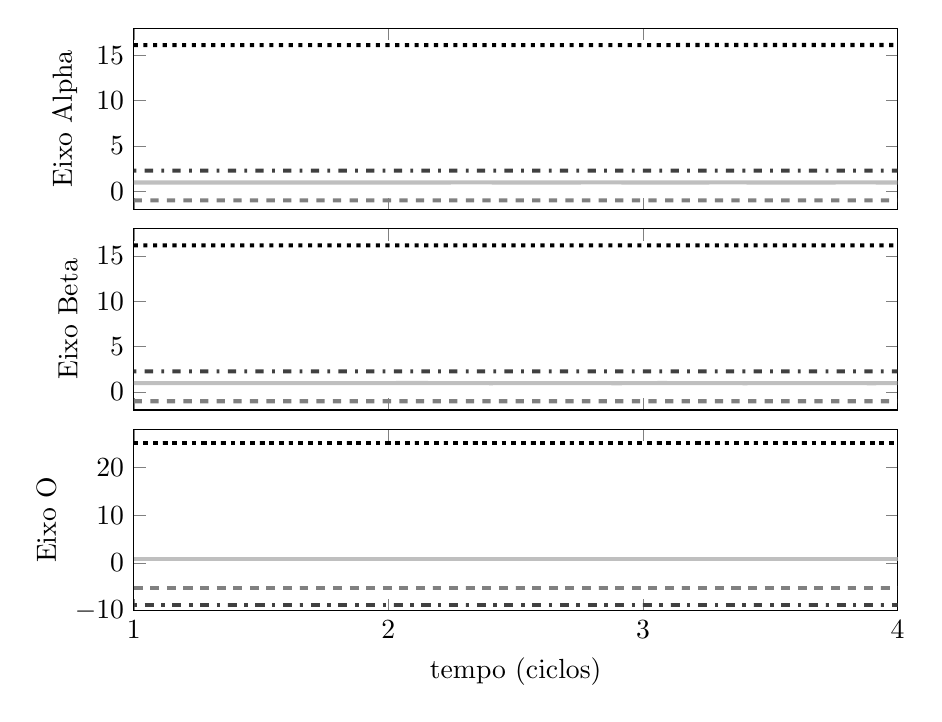
\begin{tikzpicture}

\begin{axis}[%
width=0.8\textwidth,
height=0.189701500343624\textwidth,
scale only axis,
xmin=0.316666666666667,
xmax=0.366666666666667,
xtick={0.316666666666667,0.333333333333333,0.35,0.366666666666667},
xticklabels={\empty},
ymin=-2,
ymax=18,
ytick={ 0,  5, 10, 15},
ylabel={Eixo Beta},
name=plot2,
scaled x ticks = false,
legend columns=-1,
legend style={/tikz/every even column/.append style={column sep=0.3cm}},
legend style={font=\footnotesize}
]
\addplot [color=lightgray,solid,line width=1.5pt,forget plot]
  table[row sep=crcr]{0.316658333333333	0.97043721996195\\
0.3167	0.970436358706691\\
0.316741666666667	0.970436358706691\\
0.316783333333333	0.970435592808439\\
0.316825	0.970435592808439\\
0.316866666666667	0.970434918056243\\
0.316908333333333	0.970434918056243\\
0.31695	0.970434330318112\\
0.316991666666667	0.970434330318112\\
0.317033333333333	0.970433825496951\\
0.317075	0.970433825496951\\
0.317116666666667	0.970433399492092\\
0.317158333333333	0.970433399492092\\
0.3172	0.970433048177814\\
0.317241666666667	0.970433048177814\\
0.317283333333333	0.970432767402266\\
0.317325	0.970432767402266\\
0.317366666666667	0.970432553004264\\
0.317408333333333	0.970432553004264\\
0.31745	0.970432400842131\\
0.317491666666667	0.970432400842131\\
0.317533333333333	0.970432306827843\\
0.317575	0.970432306827843\\
0.317616666666667	0.970432266960474\\
0.317658333333333	0.970432266960474\\
0.3177	0.970432277354792\\
0.317741666666667	0.970432277354792\\
0.317783333333333	0.970432334262824\\
0.317825	0.970432334262824\\
0.317866666666667	0.970432434088099\\
0.317908333333333	0.970432434088099\\
0.31795	0.970432573393534\\
0.317991666666667	0.970432573393534\\
0.318033333333333	0.970432748904596\\
0.318075	0.970432748904596\\
0.318116666666667	0.970432957509533\\
0.318158333333333	0.970432957509533\\
0.3182	0.970433196258189\\
0.318241666666667	0.970433196258189\\
0.318283333333333	0.970433462360463\\
0.318325	0.970433462360463\\
0.318366666666667	0.970433753184959\\
0.318408333333333	0.970433753184959\\
0.31845	0.970434066257974\\
0.318491666666667	0.970434066257974\\
0.318533333333333	0.970434399262647\\
0.318575	0.970434399262647\\
0.318616666666667	0.970434750037975\\
0.318658333333333	0.970434750037975\\
0.3187	0.970435116577406\\
0.318741666666667	0.970435116577406\\
0.318783333333333	0.97043549702676\\
0.318825	0.97043549702676\\
0.318866666666667	0.97043588968139\\
0.318908333333333	0.97043588968139\\
0.31895	0.970436292982595\\
0.318991666666667	0.970436292982595\\
0.319033333333333	0.970436705513386\\
0.319075	0.970436705513386\\
0.319116666666667	0.970437125993791\\
0.319158333333333	0.970437125993791\\
0.3192	0.970437553275866\\
0.319241666666667	0.970437553275866\\
0.319283333333333	0.970437986338605\\
0.319325	0.970437986338605\\
0.319366666666667	0.970438424282876\\
0.319408333333333	0.970438424282876\\
0.31945	0.970438866326497\\
0.319491666666667	0.970438866326497\\
0.319533333333333	0.97043931179951\\
0.319575	0.97043931179951\\
0.319616666666667	0.970439760139689\\
0.319658333333333	0.970439760139689\\
0.3197	0.970440210888314\\
0.319741666666667	0.970440210888314\\
0.319783333333333	0.970440663686211\\
0.319825	0.970440663686211\\
0.319866666666667	0.970441118270085\\
0.319908333333333	0.970441118270085\\
0.31995	0.970441574469177\\
0.319991666666667	0.970441574469177\\
0.320033333333333	0.970442032202265\\
0.320075	0.970442032202265\\
0.320116666666667	0.970442491475084\\
0.320158333333333	0.970442491475084\\
0.3202	0.970442952378189\\
0.320241666666667	0.970442952378189\\
0.320283333333333	0.970443415085359\\
0.320325	0.970443415085359\\
0.320366666666667	0.970443879852587\\
0.320408333333333	0.970443879852587\\
0.32045	0.970444347017744\\
0.320491666666667	0.970444347017744\\
0.320533333333333	0.970444817000997\\
0.320575	0.970444817000997\\
0.320616666666667	0.970445290306078\\
0.320658333333333	0.970445290306078\\
0.3207	0.970445767522508\\
0.320741666666667	0.970445767522508\\
0.320783333333333	0.970446249328905\\
0.320825	0.970446249328905\\
0.320866666666667	0.970446736497523\\
0.320908333333333	0.970446736497523\\
0.32095	0.970447229900211\\
0.320991666666667	0.970447229900211\\
0.321033333333333	0.970447730516016\\
0.321075	0.970447730516016\\
0.321116666666667	0.970448239440708\\
0.321158333333333	0.970448239440708\\
0.3212	0.970448757898565\\
0.321241666666667	0.970448757898565\\
0.321283333333333	0.970449287255117\\
0.321325	0.970449287255117\\
0.321366666666667	0.970449829034775\\
0.321408333333333	0.970449829034775\\
0.32145	0.970450384944168\\
0.321491666666667	0.970450384944168\\
0.321533333333333	0.970450956898191\\
0.321575	0.970450956898191\\
0.321616666666667	0.970451547051789\\
0.321658333333333	0.970451547051789\\
0.3217	0.970452157838907\\
0.321741666666667	0.970452157838907\\
0.321783333333333	0.970452792020252\\
0.321825	0.970452792020252\\
0.321866666666667	0.970453452742033\\
0.321908333333333	0.970453452742033\\
0.32195	0.970454143608473\\
0.321991666666667	0.970454143608473\\
0.322033333333333	0.970454868771685\\
0.322075	0.970454868771685\\
0.322116666666667	0.970455633043542\\
0.322158333333333	0.970455633043542\\
0.3222	0.970456442035388\\
0.322241666666667	0.970456442035388\\
0.322283333333333	0.970457302332857\\
0.322325	0.970457302332857\\
0.322366666666667	0.970458221714429\\
0.322408333333333	0.970458221714429\\
0.32245	0.97045920942283\\
0.322491666666667	0.97045920942283\\
0.322533333333333	0.97046027649605\\
0.322575	0.97046027649605\\
0.322616666666667	0.970461436154189\\
0.322658333333333	0.970461436154189\\
0.3227	0.970462704205603\\
0.322741666666667	0.970462704205603\\
0.322783333333333	0.970464099343308\\
0.322825	0.970464099343308\\
0.322866666666667	0.970465642944787\\
0.322908333333333	0.970465642944787\\
0.32295	0.970467357251532\\
0.322991666666667	0.970467357251532\\
0.323033333333333	0.970469258583928\\
0.323075	0.970469258583928\\
0.323116666666667	0.970471335019103\\
0.323158333333333	0.970471335019103\\
0.3232	0.970473348318116\\
0.323241666666667	0.970473348318116\\
0.323283333333333	0.970474626904486\\
0.323325	0.970474626904486\\
0.323366666666667	0.970474374243411\\
0.323408333333333	0.970474374243411\\
0.32345	0.970472573672318\\
0.323491666666667	0.970472573672318\\
0.323533333333333	0.970469948388625\\
0.323575	0.970469948388625\\
0.323616666666667	0.970467114613926\\
0.323658333333333	0.970467114613926\\
0.3237	0.970464337421047\\
0.323741666666667	0.970464337421047\\
0.323783333333333	0.970461683786388\\
0.323825	0.970461683786388\\
0.323866666666667	0.970459156489005\\
0.323908333333333	0.970459156489005\\
0.32395	0.970456747819866\\
0.323991666666667	0.970456747819866\\
0.324033333333333	0.970454453309765\\
0.324075	0.970454453309765\\
0.324116666666667	0.97045227287176\\
0.324158333333333	0.97045227287176\\
0.3242	0.970450209128296\\
0.324241666666667	0.970450209128296\\
0.324283333333333	0.970448265549337\\
0.324325	0.970448265549337\\
0.324366666666667	0.970446445042454\\
0.324408333333333	0.970446445042454\\
0.32445	0.970444749125981\\
0.324491666666667	0.970444749125981\\
0.324533333333333	0.970443177632723\\
0.324575	0.970443177632723\\
0.324616666666667	0.97044172880593\\
0.324658333333333	0.97044172880593\\
0.3247	0.97044039962421\\
0.324741666666667	0.97044039962421\\
0.324783333333333	0.970439186208874\\
0.324825	0.970439186208874\\
0.324866666666667	0.970438084206409\\
0.324908333333333	0.970438084206409\\
0.32495	0.970437089084224\\
0.324991666666667	0.970437089084224\\
0.325033333333333	0.970436196318331\\
0.325075	0.970436196318331\\
0.325116666666667	0.970435401481262\\
0.325158333333333	0.970435401481262\\
0.3252	0.970434700255544\\
0.325241666666667	0.970434700255544\\
0.325283333333333	0.970434088403698\\
0.325325	0.970434088403698\\
0.325366666666667	0.970433561723097\\
0.325408333333333	0.970433561723097\\
0.32545	0.970433116006485\\
0.325491666666667	0.970433116006485\\
0.325533333333333	0.970432747019942\\
0.325575	0.970432747019942\\
0.325616666666667	0.970432450501775\\
0.325658333333333	0.970432450501775\\
0.3257	0.970432222179772\\
0.325741666666667	0.970432222179772\\
0.325783333333333	0.970432057800854\\
0.325825	0.970432057800854\\
0.325866666666667	0.970431953166174\\
0.325908333333333	0.970431953166174\\
0.32595	0.970431904165525\\
0.325991666666667	0.970431904165525\\
0.326033333333333	0.970431906806762\\
0.326075	0.970431906806762\\
0.326116666666667	0.970431957238012\\
0.326158333333333	0.970431957238012\\
0.3262	0.970432051762366\\
0.326241666666667	0.970432051762366\\
0.326283333333333	0.970432186846018\\
0.326325	0.970432186846018\\
0.326366666666667	0.970432359121564\\
0.326408333333333	0.970432359121564\\
0.32645	0.97043256538827\\
0.326491666666667	0.97043256538827\\
0.326533333333333	0.970432802610885\\
0.326575	0.970432802610885\\
0.326616666666667	0.970433067918077\\
0.326658333333333	0.970433067918077\\
0.3267	0.970433358601067\\
0.326741666666667	0.970433358601067\\
0.326783333333333	0.970433672112601\\
0.326825	0.970433672112601\\
0.326866666666667	0.970434006066087\\
0.326908333333333	0.970434006066087\\
0.32695	0.970434358234596\\
0.326991666666667	0.970434358234596\\
0.327033333333333	0.970434726549414\\
0.327075	0.970434726549414\\
0.327116666666667	0.970435109097919\\
0.327158333333333	0.970435109097919\\
0.3272	0.970435504120658\\
0.327241666666667	0.970435504120658\\
0.327283333333333	0.970435910007656\\
0.327325	0.970435910007656\\
0.327366666666667	0.970436325294062\\
0.327408333333333	0.970436325294062\\
0.32745	0.970436748655303\\
0.327491666666667	0.970436748655303\\
0.327533333333333	0.970437178901951\\
0.327575	0.970437178901951\\
0.327616666666667	0.970437614974456\\
0.327658333333333	0.970437614974456\\
0.3277	0.970438055937924\\
0.327741666666667	0.970438055937924\\
0.327783333333333	0.970438500977014\\
0.327825	0.970438500977014\\
0.327866666666667	0.970438949391041\\
0.327908333333333	0.970438949391041\\
0.32795	0.970439400589312\\
0.327991666666667	0.970439400589312\\
0.328033333333333	0.970439854086724\\
0.328075	0.970439854086724\\
0.328116666666667	0.97044030949963\\
0.328158333333333	0.97044030949963\\
0.3282	0.970440766541997\\
0.328241666666667	0.970440766541997\\
0.328283333333333	0.970441225021877\\
0.328325	0.970441225021877\\
0.328366666666667	0.970441684838236\\
0.328408333333333	0.970441684838236\\
0.32845	0.970442145978184\\
0.328491666666667	0.970442145978184\\
0.328533333333333	0.970442608514653\\
0.328575	0.970442608514653\\
0.328616666666667	0.970443072604613\\
0.328658333333333	0.970443072604613\\
0.3287	0.970443538487861\\
0.328741666666667	0.970443538487861\\
0.328783333333333	0.970444006486495\\
0.328825	0.970444006486495\\
0.328866666666667	0.970444477005118\\
0.328908333333333	0.970444477005118\\
0.32895	0.970444950531897\\
0.328991666666667	0.970444950531897\\
0.329033333333333	0.970445427640563\\
0.329075	0.970445427640563\\
0.329116666666667	0.970445908993475\\
0.329158333333333	0.970445908993475\\
0.3292	0.970446395345909\\
0.329241666666667	0.970446395345909\\
0.329283333333333	0.970446887551736\\
0.329325	0.970446887551736\\
0.329366666666667	0.970447386570722\\
0.329408333333333	0.970447386570722\\
0.32945	0.970447893477714\\
0.329491666666667	0.970447893477714\\
0.329533333333333	0.970448409474047\\
0.329575	0.970448409474047\\
0.329616666666667	0.970448935899864\\
0.329658333333333	0.970448935899864\\
0.3297	0.970449474251262\\
0.329741666666667	0.970449474251262\\
0.329783333333333	0.970450026203047\\
0.329825	0.970450026203047\\
0.329866666666667	0.970450593634111\\
0.329908333333333	0.970450593634111\\
0.32995	0.970451178658432\\
0.329991666666667	0.970451178658432\\
0.330033333333333	0.970451783663083\\
0.330075	0.970451783663083\\
0.330116666666667	0.970452411354861\\
0.330158333333333	0.970452411354861\\
0.3302	0.970453064817657\\
0.330241666666667	0.970453064817657\\
0.330283333333333	0.97045374758329\\
0.330325	0.97045374758329\\
0.330366666666667	0.97045446371932\\
0.330408333333333	0.97045446371932\\
0.33045	0.970455217938359\\
0.330491666666667	0.970455217938359\\
0.330533333333333	0.970456015734584\\
0.330575	0.970456015734584\\
0.330616666666667	0.970456863554561\\
0.330658333333333	0.970456863554561\\
0.3307	0.970457769010778\\
0.330741666666667	0.970457769010778\\
0.330783333333333	0.970458741146766\\
0.330825	0.970458741146766\\
0.330866666666667	0.970459790760365\\
0.330908333333333	0.970459790760365\\
0.33095	0.970460930781311\\
0.330991666666667	0.970460930781311\\
0.331033333333333	0.970462176667188\\
0.331075	0.970462176667188\\
0.331116666666667	0.970463546691103\\
0.331158333333333	0.970463546691103\\
0.3312	0.970465061741802\\
0.331241666666667	0.970465061741802\\
0.331283333333333	0.970466743535177\\
0.331325	0.970466743535177\\
0.331366666666667	0.970468607961243\\
0.331408333333333	0.970468607961243\\
0.33145	0.970470643213183\\
0.331491666666667	0.970470643213183\\
0.331533333333333	0.970472615704777\\
0.331575	0.970472615704777\\
0.331616666666667	0.970473867713727\\
0.331658333333333	0.970473867713727\\
0.3317	0.970473619993488\\
0.331741666666667	0.970473619993488\\
0.331783333333333	0.970471857439701\\
0.331825	0.970471857439701\\
0.331866666666667	0.970469288642677\\
0.331908333333333	0.970469288642677\\
0.33195	0.970466516731413\\
0.331991666666667	0.970466516731413\\
0.332033333333333	0.970463800908304\\
0.332075	0.970463800908304\\
0.332116666666667	0.970461206531781\\
0.332158333333333	0.970461206531781\\
0.3322	0.970458736205245\\
0.332241666666667	0.970458736205245\\
0.332283333333333	0.970456382316685\\
0.332325	0.970456382316685\\
0.332366666666667	0.970454140450355\\
0.332408333333333	0.970454140450355\\
0.33245	0.97045201049146\\
0.332491666666667	0.97045201049146\\
0.332533333333333	0.970449994982174\\
0.332575	0.970449994982174\\
0.332616666666667	0.970448097296241\\
0.332658333333333	0.970448097296241\\
0.3327	0.970446320257846\\
0.332741666666667	0.970446320257846\\
0.332783333333333	0.970444665332178\\
0.332825	0.970444665332178\\
0.332866666666667	0.970443132335721\\
0.332908333333333	0.970443132335721\\
0.33295	0.970441719530581\\
0.332991666666667	0.970441719530581\\
0.333033333333333	0.970440423942802\\
0.333075	0.970440423942802\\
0.333116666666667	0.970439241761191\\
0.333158333333333	0.970439241761191\\
0.3332	0.970438168711639\\
0.333241666666667	0.970438168711639\\
0.333283333333333	0.970437200346429\\
0.333325	0.970437200346429\\
0.333366666666667	0.970436332227711\\
0.333408333333333	0.970436332227711\\
0.33345	0.970435560013326\\
0.333491666666667	0.970435560013326\\
0.333533333333333	0.971648858949127\\
0.333575	0.971648858949127\\
0.333616666666667	0.972551835611606\\
0.333658333333333	0.972551835611606\\
0.3337	0.973207764997182\\
0.333741666666667	0.973207764997182\\
0.333783333333333	0.973720077134853\\
0.333825	0.973720077134853\\
0.333866666666667	0.974138678563171\\
0.333908333333333	0.974138678563171\\
0.33395	0.97448861200456\\
0.333991666666667	0.97448861200456\\
0.334033333333333	0.974785425419367\\
0.334075	0.974785425419367\\
0.334116666666667	0.975038737431379\\
0.334158333333333	0.975038737431379\\
0.3342	0.975253422953218\\
0.334241666666667	0.975253422953218\\
0.334283333333333	0.975431090751057\\
0.334325	0.975431090751057\\
0.334366666666667	0.975571729224647\\
0.334408333333333	0.975571729224647\\
0.33445	0.975675085962529\\
0.334491666666667	0.975675085962529\\
0.334533333333333	0.975741568319722\\
0.334575	0.975741568319722\\
0.334616666666667	0.975772645258401\\
0.334658333333333	0.975772645258401\\
0.3347	0.975770841164928\\
0.334741666666667	0.975770841164928\\
0.334783333333333	0.975739462345535\\
0.334825	0.975739462345535\\
0.334866666666667	0.97568220308738\\
0.334908333333333	0.97568220308738\\
0.33495	0.975602754094434\\
0.334991666666667	0.975602754094434\\
0.335033333333333	0.975504495724003\\
0.335075	0.975504495724003\\
0.335116666666667	0.975390314683187\\
0.335158333333333	0.975390314683187\\
0.3352	0.97526254538269\\
0.335241666666667	0.97526254538269\\
0.335283333333333	0.975123011403737\\
0.335325	0.975123011403737\\
0.335366666666667	0.974973129879909\\
0.335408333333333	0.974973129879909\\
0.33545	0.974814040368281\\
0.335491666666667	0.974814040368281\\
0.335533333333333	0.974646726603347\\
0.335575	0.974646726603347\\
0.335616666666667	0.974472110514347\\
0.335658333333333	0.974472110514347\\
0.3357	0.974291109577703\\
0.335741666666667	0.974291109577703\\
0.335783333333333	0.974104658457263\\
0.335825	0.974104658457263\\
0.335866666666667	0.973913702574732\\
0.335908333333333	0.973913702574732\\
0.33595	0.973719174414939\\
0.335991666666667	0.973719174414939\\
0.336033333333333	0.9735219634573\\
0.336075	0.9735219634573\\
0.336116666666667	0.973322888548348\\
0.336158333333333	0.973322888548348\\
0.3362	0.973122678347426\\
0.336241666666667	0.973122678347426\\
0.336283333333333	0.972921962142289\\
0.336325	0.972921962142289\\
0.336366666666667	0.972721270540403\\
0.336408333333333	0.972721270540403\\
0.33645	0.972521043677767\\
0.336491666666667	0.972521043677767\\
0.336533333333333	0.97232164373873\\
0.336575	0.97232164373873\\
0.336616666666667	0.97212336861283\\
0.336658333333333	0.97212336861283\\
0.3367	0.971926464162576\\
0.336741666666667	0.971926464162576\\
0.336783333333333	0.971731133532888\\
0.336825	0.971731133532888\\
0.336866666666667	0.971537542921919\\
0.336908333333333	0.971537542921919\\
0.33695	0.971345824051992\\
0.336991666666667	0.971345824051992\\
0.337033333333333	0.971156074117405\\
0.337075	0.971156074117405\\
0.337116666666667	0.970968354218081\\
0.337158333333333	0.970968354218081\\
0.3372	0.970782687255614\\
0.337241666666667	0.970782687255614\\
0.337283333333333	0.970599056051596\\
0.337325	0.970599056051596\\
0.337366666666667	0.970417402139909\\
0.337408333333333	0.970417402139909\\
0.33745	0.970237625369066\\
0.337491666666667	0.970237625369066\\
0.337533333333333	0.970059584189185\\
0.337575	0.970059584189185\\
0.337616666666667	0.96988309632448\\
0.337658333333333	0.96988309632448\\
0.3377	0.969707939453289\\
0.337741666666667	0.969707939453289\\
0.337783333333333	0.969533851520112\\
0.337825	0.969533851520112\\
0.337866666666667	0.969360530361959\\
0.337908333333333	0.969360530361959\\
0.33795	0.96918763241424\\
0.337991666666667	0.96918763241424\\
0.338033333333333	0.969014770341763\\
0.338075	0.969014770341763\\
0.338116666666667	0.968841509704726\\
0.338158333333333	0.968841509704726\\
0.3382	0.968667364944703\\
0.338241666666667	0.968667364944703\\
0.338283333333333	0.968491792226096\\
0.338325	0.968491792226096\\
0.338366666666667	0.968314181869248\\
0.338408333333333	0.968314181869248\\
0.33845	0.968133849053945\\
0.338491666666667	0.968133849053945\\
0.338533333333333	0.967950022355481\\
0.338575	0.967950022355481\\
0.338616666666667	0.967761829596934\\
0.338658333333333	0.967761829596934\\
0.3387	0.967568280311102\\
0.338741666666667	0.967568280311102\\
0.338783333333333	0.967368243882625\\
0.338825	0.967368243882625\\
0.338866666666667	0.967160422188105\\
0.338908333333333	0.967160422188105\\
0.33895	0.966943315269325\\
0.338991666666667	0.966943315269325\\
0.339033333333333	0.966715178289778\\
0.339075	0.966715178289778\\
0.339116666666667	0.966473967838326\\
0.339158333333333	0.966473967838326\\
0.3392	0.966217275837303\\
0.339241666666667	0.966217275837303\\
0.339283333333333	0.965942250621072\\
0.339325	0.965942250621072\\
0.339366666666667	0.965645509068642\\
0.339408333333333	0.965645509068642\\
0.33945	0.965323055947907\\
0.339491666666667	0.965323055947907\\
0.339533333333333	0.964970260218407\\
0.339575	0.964970260218407\\
0.339616666666667	0.964582030813449\\
0.339658333333333	0.964582030813449\\
0.3397	0.964153600730688\\
0.339741666666667	0.964153600730688\\
0.339783333333333	0.963683141276039\\
0.339825	0.963683141276039\\
0.339866666666667	0.963180713548748\\
0.339908333333333	0.963180713548748\\
0.33995	0.962743221931403\\
0.339991666666667	0.962743221931403\\
0.340033333333333	0.962557941035935\\
0.340075	0.962557941035935\\
0.340116666666667	0.962763377463747\\
0.340158333333333	0.962763377463747\\
0.3402	0.963273642199086\\
0.340241666666667	0.963273642199086\\
0.340283333333333	0.963908110712242\\
0.340325	0.963908110712242\\
0.340366666666667	0.964554989557809\\
0.340408333333333	0.964554989557809\\
0.34045	0.965175580876337\\
0.340491666666667	0.965175580876337\\
0.340533333333333	0.965763532636179\\
0.340575	0.965763532636179\\
0.340616666666667	0.966321146142632\\
0.340658333333333	0.966321146142632\\
0.3407	0.966851430234263\\
0.340741666666667	0.966851430234263\\
0.340783333333333	0.967356394568855\\
0.340825	0.967356394568855\\
0.340866666666667	0.967837036696378\\
0.340908333333333	0.967837036696378\\
0.34095	0.968293661219689\\
0.340991666666667	0.968293661219689\\
0.341033333333333	0.968726209357149\\
0.341075	0.968726209357149\\
0.341116666666667	0.969134520970968\\
0.341158333333333	0.969134520970968\\
0.3412	0.969518508430739\\
0.341241666666667	0.969518508430739\\
0.341283333333333	0.969878245891628\\
0.341325	0.969878245891628\\
0.341366666666667	0.970213991385115\\
0.341408333333333	0.970213991385115\\
0.34145	0.970526164701536\\
0.341491666666667	0.970526164701536\\
0.341533333333333	0.97081530333607\\
0.341575	0.97081530333607\\
0.341616666666667	0.971082014269825\\
0.341658333333333	0.971082014269825\\
0.3417	0.971326933286298\\
0.341741666666667	0.971326933286298\\
0.341783333333333	0.971550697532474\\
0.341825	0.971550697532474\\
0.341866666666667	0.971753932167101\\
0.341908333333333	0.971753932167101\\
0.34195	0.9719372486824\\
0.341991666666667	0.9719372486824\\
0.342033333333333	0.972101250875096\\
0.342075	0.972101250875096\\
0.342116666666667	0.972246544205042\\
0.342158333333333	0.972246544205042\\
0.3422	0.972373744983395\\
0.342241666666667	0.972373744983395\\
0.342283333333333	0.972483487017517\\
0.342325	0.972483487017517\\
0.342366666666667	0.972576424611567\\
0.342408333333333	0.972576424611567\\
0.34245	0.972653231901819\\
0.342491666666667	0.972653231901819\\
0.342533333333333	0.972714599245227\\
0.342575	0.972714599245227\\
0.342616666666667	0.972761227744934\\
0.342658333333333	0.972761227744934\\
0.3427	0.97279382303673\\
0.342741666666667	0.97279382303673\\
0.342783333333333	0.972813089272279\\
0.342825	0.972813089272279\\
0.342866666666667	0.972819723927495\\
0.342908333333333	0.972819723927495\\
0.34295	0.972814413734991\\
0.342991666666667	0.972814413734991\\
0.343033333333333	0.972797831758329\\
0.343075	0.972797831758329\\
0.343116666666667	0.97277063543143\\
0.343158333333333	0.97277063543143\\
0.3432	0.972733465288513\\
0.343241666666667	0.972733465288513\\
0.343283333333333	0.972686944096195\\
0.343325	0.972686944096195\\
0.343366666666667	0.972631676145526\\
0.343408333333333	0.972631676145526\\
0.34345	0.972568246539458\\
0.343491666666667	0.972568246539458\\
0.343533333333333	0.972497220395148\\
0.343575	0.972497220395148\\
0.343616666666667	0.972419141952143\\
0.343658333333333	0.972419141952143\\
0.3437	0.972334533626447\\
0.343741666666667	0.972334533626447\\
0.343783333333333	0.972243895074241\\
0.343825	0.972243895074241\\
0.343866666666667	0.972147702330704\\
0.343908333333333	0.972147702330704\\
0.34395	0.972046407075359\\
0.343991666666667	0.972046407075359\\
0.344033333333333	0.971940436053389\\
0.344075	0.971940436053389\\
0.344116666666667	0.971830190659022\\
0.344158333333333	0.971830190659022\\
0.3442	0.971716046667481\\
0.344241666666667	0.971716046667481\\
0.344283333333333	0.971598354088828\\
0.344325	0.971598354088828\\
0.344366666666667	0.971477437110907\\
0.344408333333333	0.971477437110907\\
0.34445	0.971353594098613\\
0.344491666666667	0.971353594098613\\
0.344533333333333	0.97122709762098\\
0.344575	0.97122709762098\\
0.344616666666667	0.971098194483956\\
0.344658333333333	0.971098194483956\\
0.3447	0.970967105753223\\
0.344741666666667	0.970967105753223\\
0.344783333333333	0.97083402675669\\
0.344825	0.97083402675669\\
0.344866666666667	0.970699127059441\\
0.344908333333333	0.970699127059441\\
0.34495	0.970562550404825\\
0.344991666666667	0.970562550404825\\
0.345033333333333	0.970424414614293\\
0.345075	0.970424414614293\\
0.345116666666667	0.970284811435954\\
0.345158333333333	0.970284811435954\\
0.3452	0.970143806328325\\
0.345241666666667	0.970143806328325\\
0.345283333333333	0.970001438161806\\
0.345325	0.970001438161806\\
0.345366666666667	0.96985771881637\\
0.345408333333333	0.96985771881637\\
0.34545	0.969712632650021\\
0.345491666666667	0.969712632650021\\
0.345533333333333	0.969566135808537\\
0.345575	0.969566135808537\\
0.345616666666667	0.96941815534272\\
0.345658333333333	0.96941815534272\\
0.3457	0.96926858809443\\
0.345741666666667	0.96926858809443\\
0.345783333333333	0.969117299306608\\
0.345825	0.969117299306608\\
0.345866666666667	0.968964120904819\\
0.345908333333333	0.968964120904819\\
0.34595	0.968808849387983\\
0.345991666666667	0.968808849387983\\
0.346033333333333	0.968651243253345\\
0.346075	0.968651243253345\\
0.346116666666667	0.968491019864569\\
0.346158333333333	0.968491019864569\\
0.3462	0.968327851651247\\
0.346241666666667	0.968327851651247\\
0.346283333333333	0.968161361501957\\
0.346325	0.968161361501957\\
0.346366666666667	0.967991117179635\\
0.346408333333333	0.967991117179635\\
0.34645	0.967816625010012\\
0.346491666666667	0.967816625010012\\
0.346533333333333	0.967637322060543\\
0.346575	0.967637322060543\\
0.346616666666667	0.967452565308079\\
0.346658333333333	0.967452565308079\\
0.3467	0.967261619492175\\
0.346741666666667	0.967261619492175\\
0.346783333333333	0.967063642238294\\
0.346825	0.967063642238294\\
0.346866666666667	0.96685766572051\\
0.346908333333333	0.96685766572051\\
0.34695	0.966642574005765\\
0.346991666666667	0.966642574005765\\
0.347033333333333	0.966417074974842\\
0.347075	0.966417074974842\\
0.347116666666667	0.96617966541294\\
0.347158333333333	0.96617966541294\\
0.3472	0.965928587517468\\
0.347241666666667	0.965928587517468\\
0.347283333333333	0.965661774720542\\
0.347325	0.965661774720542\\
0.347366666666667	0.965376784497903\\
0.347408333333333	0.965376784497903\\
0.34745	0.965070716086806\\
0.347491666666667	0.965070716086806\\
0.347533333333333	0.964740112668365\\
0.347575	0.964740112668365\\
0.347616666666667	0.964380852893748\\
0.347658333333333	0.964380852893748\\
0.3477	0.963988051632603\\
0.347741666666667	0.963988051632603\\
0.347783333333333	0.963556030534422\\
0.347825	0.963556030534422\\
0.347866666666667	0.963078530534428\\
0.347908333333333	0.963078530534428\\
0.34795	0.962549655920968\\
0.347991666666667	0.962549655920968\\
0.348033333333333	0.9619670001309\\
0.348075	0.9619670001309\\
0.348116666666667	0.961341555134438\\
0.348158333333333	0.961341555134438\\
0.3482	0.960788377948118\\
0.348241666666667	0.960788377948118\\
0.348283333333333	0.960537072510808\\
0.348325	0.960537072510808\\
0.348366666666667	0.96077034870615\\
0.348408333333333	0.96077034870615\\
0.34845	0.961397599057846\\
0.348491666666667	0.961397599057846\\
0.348533333333333	0.962195102191525\\
0.348575	0.962195102191525\\
0.348616666666667	0.963016612349346\\
0.348658333333333	0.963016612349346\\
0.3487	0.963808716689139\\
0.348741666666667	0.963808716689139\\
0.348783333333333	0.964561247765427\\
0.348825	0.964561247765427\\
0.348866666666667	0.965276306971616\\
0.348908333333333	0.965276306971616\\
0.34895	0.965957395319728\\
0.348991666666667	0.965957395319728\\
0.349033333333333	0.966606924228981\\
0.349075	0.966606924228981\\
0.349116666666667	0.967226090899207\\
0.349158333333333	0.967226090899207\\
0.3492	0.967815243178363\\
0.349241666666667	0.967815243178363\\
0.349283333333333	0.968374279653504\\
0.349325	0.968374279653504\\
0.349366666666667	0.968902974216558\\
0.349408333333333	0.968902974216558\\
0.34945	0.969401194366304\\
0.349491666666667	0.969401194366304\\
0.349533333333333	0.969869014882489\\
0.349575	0.969869014882489\\
0.349616666666667	0.97030674708039\\
0.349658333333333	0.97030674708039\\
0.3497	0.97071491179284\\
0.349741666666667	0.97071491179284\\
0.349783333333333	0.971094183927962\\
0.349825	0.971094183927962\\
0.349866666666667	0.971445331102536\\
0.349908333333333	0.971445331102536\\
0.34995	0.971769161333504\\
0.349991666666667	0.971769161333504\\
0.350033333333333	0.972066487237209\\
0.350075	0.972066487237209\\
0.350116666666667	0.972338108007384\\
0.350158333333333	0.972338108007384\\
0.3502	0.972584806270275\\
0.350241666666667	0.972584806270275\\
0.350283333333333	0.9728073548172\\
0.350325	0.9728073548172\\
0.350366666666667	0.973006527860163\\
0.350408333333333	0.973006527860163\\
0.35045	0.97318311230518\\
0.350491666666667	0.97318311230518\\
0.350533333333333	0.973337916010511\\
0.350575	0.973337916010511\\
0.350616666666667	0.97347177159193\\
0.350658333333333	0.97347177159193\\
0.3507	0.973585535699788\\
0.350741666666667	0.973585535699788\\
0.350783333333333	0.973680084631658\\
0.350825	0.973680084631658\\
0.350866666666667	0.973756307614418\\
0.350908333333333	0.973756307614418\\
0.35095	0.973815099150894\\
0.350991666666667	0.973815099150894\\
0.351033333333333	0.973857351598739\\
0.351075	0.973857351598739\\
0.351116666666667	0.973883948769797\\
0.351158333333333	0.973883948769797\\
0.3512	0.973895760928848\\
0.351241666666667	0.973895760928848\\
0.351283333333333	0.973893641219893\\
0.351325	0.973893641219893\\
0.351366666666667	0.973878423304609\\
0.351408333333333	0.973878423304609\\
0.35145	0.973850919873737\\
0.351491666666667	0.973850919873737\\
0.351533333333333	0.973811921673314\\
0.351575	0.973811921673314\\
0.351616666666667	0.973762196743484\\
0.351658333333333	0.973762196743484\\
0.3517	0.973702489663175\\
0.351741666666667	0.973702489663175\\
0.351783333333333	0.973633520697664\\
0.351825	0.973633520697664\\
0.351866666666667	0.973555984834914\\
0.351908333333333	0.973555984834914\\
0.35195	0.973470550757728\\
0.351991666666667	0.973470550757728\\
0.352033333333333	0.973377859828882\\
0.352075	0.973377859828882\\
0.352116666666667	0.973278525169281\\
0.352158333333333	0.973278525169281\\
0.3522	0.973173130892697\\
0.352241666666667	0.973173130892697\\
0.352283333333333	0.973062231534188\\
0.352325	0.973062231534188\\
0.352366666666667	0.972946351681092\\
0.352408333333333	0.972946351681092\\
0.35245	0.972825985791745\\
0.352491666666667	0.972825985791745\\
0.352533333333333	0.972701598171142\\
0.352575	0.972701598171142\\
0.352616666666667	0.972573623065425\\
0.352658333333333	0.972573623065425\\
0.3527	0.972442464837294\\
0.352741666666667	0.972442464837294\\
0.352783333333333	0.972308498189818\\
0.352825	0.972308498189818\\
0.352866666666667	0.972172068414187\\
0.352908333333333	0.972172068414187\\
0.35295	0.972033491645237\\
0.352991666666667	0.972033491645237\\
0.353033333333333	0.971893055115423\\
0.353075	0.971893055115423\\
0.353116666666667	0.971751017402316\\
0.353158333333333	0.971751017402316\\
0.3532	0.971607608666504\\
0.353241666666667	0.971607608666504\\
0.353283333333333	0.971463030876194\\
0.353325	0.971463030876194\\
0.353366666666667	0.971317458012606\\
0.353408333333333	0.971317458012606\\
0.35345	0.971171036247034\\
0.353491666666667	0.971171036247034\\
0.353533333333333	0.971023884076982\\
0.353575	0.971023884076982\\
0.353616666666667	0.970876092405433\\
0.353658333333333	0.970876092405433\\
0.3537	0.970727724544334\\
0.353741666666667	0.970727724544334\\
0.353783333333333	0.97057881612078\\
0.353825	0.97057881612078\\
0.353866666666667	0.970429374861899\\
0.353908333333333	0.970429374861899\\
0.35395	0.970279380231812\\
0.353991666666667	0.970279380231812\\
0.354033333333333	0.970128782890901\\
0.354075	0.970128782890901\\
0.354116666666667	0.969977503943473\\
0.354158333333333	0.969977503943473\\
0.3542	0.969825433934529\\
0.354241666666667	0.969825433934529\\
0.354283333333333	0.969672431549141\\
0.354325	0.969672431549141\\
0.354366666666667	0.969518321958733\\
0.354408333333333	0.969518321958733\\
0.35445	0.969362894746629\\
0.354491666666667	0.969362894746629\\
0.354533333333333	0.969205901330155\\
0.354575	0.969205901330155\\
0.354616666666667	0.969047051777471\\
0.354658333333333	0.969047051777471\\
0.3547	0.968886010893059\\
0.354741666666667	0.968886010893059\\
0.354783333333333	0.968722393858097\\
0.354825	0.968722393858097\\
0.354866666666667	0.968555760623468\\
0.354908333333333	0.968555760623468\\
0.35495	0.968385607996405\\
0.354991666666667	0.968385607996405\\
0.355033333333333	0.968211360874338\\
0.355075	0.968211360874338\\
0.355116666666667	0.968032361469167\\
0.355158333333333	0.968032361469167\\
0.3552	0.967847855985232\\
0.355241666666667	0.967847855985232\\
0.355283333333333	0.967656978131575\\
0.355325	0.967656978131575\\
0.355366666666667	0.967458728665083\\
0.355408333333333	0.967458728665083\\
0.35545	0.967251949932161\\
0.355491666666667	0.967251949932161\\
0.355533333333333	0.967035294105211\\
0.355575	0.967035294105211\\
0.355616666666667	0.96680718350692\\
0.355658333333333	0.96680718350692\\
0.3557	0.966565761135913\\
0.355741666666667	0.966565761135913\\
0.355783333333333	0.966308829418209\\
0.355825	0.966308829418209\\
0.355866666666667	0.966033775751284\\
0.355908333333333	0.966033775751284\\
0.35595	0.965737485713522\\
0.355991666666667	0.965737485713522\\
0.356033333333333	0.965416251796768\\
0.356075	0.965416251796768\\
0.356116666666667	0.965065704871728\\
0.356158333333333	0.965065704871728\\
0.3562	0.964680848419151\\
0.356241666666667	0.964680848419151\\
0.356283333333333	0.96425642304089\\
0.356325	0.96425642304089\\
0.356366666666667	0.963788261022256\\
0.356408333333333	0.963788261022256\\
0.35645	0.963277649960367\\
0.356491666666667	0.963277649960367\\
0.356533333333333	0.962763374230932\\
0.356575	0.962763374230932\\
0.356616666666667	0.962386936828408\\
0.356658333333333	0.962386936828408\\
0.3567	0.96235156115393\\
0.356741666666667	0.96235156115393\\
0.356783333333333	0.962715132011066\\
0.356825	0.962715132011066\\
0.356866666666667	0.963320666260635\\
0.356908333333333	0.963320666260635\\
0.35695	0.963998138576959\\
0.356991666666667	0.963998138576959\\
0.357033333333333	0.964665369956402\\
0.357075	0.964665369956402\\
0.357116666666667	0.965299729822868\\
0.357158333333333	0.965299729822868\\
0.3572	0.965900114563002\\
0.357241666666667	0.965900114563002\\
0.357283333333333	0.966469816180699\\
0.357325	0.966469816180699\\
0.357366666666667	0.967011694173664\\
0.357408333333333	0.967011694173664\\
0.35745	0.967527444440113\\
0.357491666666667	0.967527444440113\\
0.357533333333333	0.968017823220618\\
0.357575	0.968017823220618\\
0.357616666666667	0.96848300778086\\
0.357658333333333	0.96848300778086\\
0.3577	0.968922916499335\\
0.357741666666667	0.968922916499335\\
0.357783333333333	0.969337444550679\\
0.357825	0.969337444550679\\
0.357866666666667	0.969726606878782\\
0.357908333333333	0.969726606878782\\
0.35795	0.97009059938096\\
0.357991666666667	0.97009059938096\\
0.358033333333333	0.970429799818908\\
0.358075	0.970429799818908\\
0.358116666666667	0.970744732776209\\
0.358158333333333	0.970744732776209\\
0.3582	0.971036020267481\\
0.358241666666667	0.971036020267481\\
0.358283333333333	0.971304333952506\\
0.358325	0.971304333952506\\
0.358366666666667	0.971550358425975\\
0.358408333333333	0.971550358425975\\
0.35845	0.971774769198906\\
0.358491666666667	0.971774769198906\\
0.358533333333333	0.971978224592428\\
0.358575	0.971978224592428\\
0.358616666666667	0.972161368117132\\
0.358658333333333	0.972161368117132\\
0.3587	0.97232483689012\\
0.358741666666667	0.97232483689012\\
0.358783333333333	0.972469271872084\\
0.358825	0.972469271872084\\
0.358866666666667	0.97259532671032\\
0.358908333333333	0.97259532671032\\
0.35895	0.972703673290413\\
0.358991666666667	0.972703673290413\\
0.359033333333333	0.972795003365617\\
0.359075	0.972795003365617\\
0.359116666666667	0.972870026617054\\
0.359158333333333	0.972870026617054\\
0.3592	0.972929466099244\\
0.359241666666667	0.972929466099244\\
0.359283333333333	0.972974052250993\\
0.359325	0.972974052250993\\
0.359366666666667	0.973004516578431\\
0.359408333333333	0.973004516578431\\
0.35945	0.973021585854869\\
0.359491666666667	0.973021585854869\\
0.359533333333333	0.973025977342107\\
0.359575	0.973025977342107\\
0.359616666666667	0.973018395210054\\
0.359658333333333	0.973018395210054\\
0.3597	0.972999528075137\\
0.359741666666667	0.972999528075137\\
0.359783333333333	0.972970047419237\\
0.359825	0.972970047419237\\
0.359866666666667	0.972930606589042\\
0.359908333333333	0.972930606589042\\
0.35995	0.972881840091521\\
0.359991666666667	0.972881840091521\\
0.360033333333333	0.97282436296652\\
0.360075	0.97282436296652\\
0.360116666666667	0.972758770103699\\
0.360158333333333	0.972758770103699\\
0.3602	0.972685635454403\\
0.360241666666667	0.972685635454403\\
0.360283333333333	0.97260551115411\\
0.360325	0.97260551115411\\
0.360366666666667	0.972518926610653\\
0.360408333333333	0.972518926610653\\
0.36045	0.97242638762769\\
0.360491666666667	0.97242638762769\\
0.360533333333333	0.97232837562682\\
0.360575	0.97232837562682\\
0.360616666666667	0.972225347012884\\
0.360658333333333	0.972225347012884\\
0.3607	0.972117732702924\\
0.360741666666667	0.972117732702924\\
0.360783333333333	0.972005937816376\\
0.360825	0.972005937816376\\
0.360866666666667	0.971890341506481\\
0.360908333333333	0.971890341506481\\
0.36095	0.971771296902463\\
0.360991666666667	0.971771296902463\\
0.361033333333333	0.971649131128654\\
0.361075	0.971649131128654\\
0.361116666666667	0.971524145368953\\
0.361158333333333	0.971524145368953\\
0.3612	0.971396614950672\\
0.361241666666667	0.971396614950672\\
0.361283333333333	0.971266789428732\\
0.361325	0.971266789428732\\
0.361366666666667	0.971134892657594\\
0.361408333333333	0.971134892657594\\
0.36145	0.971001122842976\\
0.361491666666667	0.971001122842976\\
0.361533333333333	0.970865652567805\\
0.361575	0.970865652567805\\
0.361616666666667	0.970728628787039\\
0.361658333333333	0.970728628787039\\
0.3617	0.970590172784328\\
0.361741666666667	0.970590172784328\\
0.361783333333333	0.970450380080569\\
0.361825	0.970450380080569\\
0.361866666666667	0.97030932028084\\
0.361908333333333	0.97030932028084\\
0.36195	0.970167036842429\\
0.361991666666667	0.970167036842429\\
0.362033333333333	0.970023546742998\\
0.362075	0.970023546742998\\
0.362116666666667	0.969878840024364\\
0.362158333333333	0.969878840024364\\
0.3622	0.969732879183796\\
0.362241666666667	0.969732879183796\\
0.362283333333333	0.9695855983809\\
0.362325	0.9695855983809\\
0.362366666666667	0.969436902423623\\
0.362408333333333	0.969436902423623\\
0.36245	0.969286665491246\\
0.362491666666667	0.969286665491246\\
0.362533333333333	0.969134729545048\\
0.362575	0.969134729545048\\
0.362616666666667	0.968980902367977\\
0.362658333333333	0.968980902367977\\
0.3627	0.968824955162702\\
0.362741666666667	0.968824955162702\\
0.362783333333333	0.968666619622136\\
0.362825	0.968666619622136\\
0.362866666666667	0.968505584367057\\
0.362908333333333	0.968505584367057\\
0.36295	0.968341490620739\\
0.362991666666667	0.968341490620739\\
0.363033333333333	0.968173926959096\\
0.363075	0.968173926959096\\
0.363116666666667	0.968002423385433\\
0.363158333333333	0.968002423385433\\
0.3632	0.967826443971447\\
0.363241666666667	0.967826443971447\\
0.363283333333333	0.967645376623545\\
0.363325	0.967645376623545\\
0.363366666666667	0.967458521637732\\
0.363408333333333	0.967458521637732\\
0.36345	0.967265077678393\\
0.363491666666667	0.967265077678393\\
0.363533333333333	0.967064124487711\\
0.363575	0.967064124487711\\
0.363616666666667	0.966854601516975\\
0.363658333333333	0.966854601516975\\
0.3637	0.966635281434992\\
0.363741666666667	0.966635281434992\\
0.363783333333333	0.966404737177826\\
0.363825	0.966404737177826\\
0.363866666666667	0.966161300867453\\
0.363908333333333	0.966161300867453\\
0.36395	0.965903012573484\\
0.363991666666667	0.965903012573484\\
0.364033333333333	0.965627556628981\\
0.364075	0.965627556628981\\
0.364116666666667	0.965332183337286\\
0.364158333333333	0.965332183337286\\
0.3642	0.965013615196673\\
0.364241666666667	0.965013615196673\\
0.364283333333333	0.96466794120584\\
0.364325	0.96466794120584\\
0.364366666666667	0.964290515533544\\
0.364408333333333	0.964290515533544\\
0.36445	0.963875911576807\\
0.364491666666667	0.963875911576807\\
0.364533333333333	0.963418077664188\\
0.364575	0.963418077664188\\
0.364616666666667	0.962911110870839\\
0.364658333333333	0.962911110870839\\
0.3647	0.96235187796569\\
0.364741666666667	0.96235187796569\\
0.364783333333333	0.961748355884677\\
0.364825	0.961748355884677\\
0.364866666666667	0.961194951845608\\
0.364908333333333	0.961194951845608\\
0.36495	0.960903389818248\\
0.364991666666667	0.960903389818248\\
0.365033333333333	0.96107189811835\\
0.365075	0.96107189811835\\
0.365116666666667	0.961645170240042\\
0.365158333333333	0.961645170240042\\
0.3652	0.962406472134593\\
0.365241666666667	0.962406472134593\\
0.365283333333333	0.96320043249184\\
0.365325	0.96320043249184\\
0.365366666666667	0.963967323367557\\
0.365408333333333	0.963967323367557\\
0.36545	0.96469505714666\\
0.365491666666667	0.96469505714666\\
0.365533333333333	0.965385567313351\\
0.365575	0.965385567313351\\
0.365616666666667	0.966042548039414\\
0.365658333333333	0.966042548039414\\
0.3657	0.966668609571715\\
0.365741666666667	0.966668609571715\\
0.365783333333333	0.967265111022754\\
0.365825	0.967265111022754\\
0.365866666666667	0.967832526770692\\
0.365908333333333	0.967832526770692\\
0.36595	0.968370847509121\\
0.365991666666667	0.968370847509121\\
0.366033333333333	0.968879906874164\\
0.366075	0.968879906874164\\
0.366116666666667	0.969359604600825\\
0.366158333333333	0.969359604600825\\
0.3662	0.969810026723854\\
0.366241666666667	0.969810026723854\\
0.366283333333333	0.970231481454978\\
0.366325	0.970231481454978\\
0.366366666666667	0.97062447778232\\
0.366408333333333	0.97062447778232\\
0.36645	0.970989674101551\\
0.366491666666667	0.970989674101551\\
0.366533333333333	0.971327819292325\\
0.366575	0.971327819292325\\
0.366616666666667	0.971639701449905\\
0.366658333333333	0.971639701449905\\
};
\addplot [color=gray,dashed,line width=1.5pt,forget plot]
  table[row sep=crcr]{0.316658333333333	-1.02797931894004\\
0.3167	-1.0279793224329\\
0.316741666666667	-1.0279793224329\\
0.316783333333333	-1.02797932543233\\
0.316825	-1.02797932543233\\
0.316866666666667	-1.02797932798806\\
0.316908333333333	-1.02797932798806\\
0.31695	-1.02797933014413\\
0.316991666666667	-1.02797933014413\\
0.317033333333333	-1.02797933193992\\
0.317075	-1.02797933193992\\
0.317116666666667	-1.02797933341104\\
0.317158333333333	-1.02797933341104\\
0.3172	-1.02797933458991\\
0.317241666666667	-1.02797933458991\\
0.317283333333333	-1.02797933550621\\
0.317325	-1.02797933550621\\
0.317366666666667	-1.02797933618718\\
0.317408333333333	-1.02797933618718\\
0.31745	-1.02797933665787\\
0.317491666666667	-1.02797933665787\\
0.317533333333333	-1.02797933694126\\
0.317575	-1.02797933694126\\
0.317616666666667	-1.02797933705843\\
0.317658333333333	-1.02797933705843\\
0.3177	-1.02797933702864\\
0.317741666666667	-1.02797933702864\\
0.317783333333333	-1.02797933686946\\
0.317825	-1.02797933686946\\
0.317866666666667	-1.02797933659693\\
0.317908333333333	-1.02797933659693\\
0.31795	-1.02797933622564\\
0.317991666666667	-1.02797933622564\\
0.318033333333333	-1.02797933576886\\
0.318075	-1.02797933576886\\
0.318116666666667	-1.02797933523867\\
0.318158333333333	-1.02797933523867\\
0.3182	-1.02797933464602\\
0.318241666666667	-1.02797933464602\\
0.318283333333333	-1.02797933400088\\
0.318325	-1.02797933400088\\
0.318366666666667	-1.02797933331226\\
0.318408333333333	-1.02797933331226\\
0.31845	-1.02797933258833\\
0.318491666666667	-1.02797933258833\\
0.318533333333333	-1.02797933183645\\
0.318575	-1.02797933183645\\
0.318616666666667	-1.02797933106326\\
0.318658333333333	-1.02797933106326\\
0.3187	-1.02797933027471\\
0.318741666666667	-1.02797933027471\\
0.318783333333333	-1.02797932947612\\
0.318825	-1.02797932947612\\
0.318866666666667	-1.02797932867225\\
0.318908333333333	-1.02797932867225\\
0.31895	-1.0279793278673\\
0.318991666666667	-1.0279793278673\\
0.319033333333333	-1.02797932706501\\
0.319075	-1.02797932706501\\
0.319116666666667	-1.02797932626865\\
0.319158333333333	-1.02797932626865\\
0.3192	-1.02797932548113\\
0.319241666666667	-1.02797932548113\\
0.319283333333333	-1.02797932470497\\
0.319325	-1.02797932470497\\
0.319366666666667	-1.02797932394236\\
0.319408333333333	-1.02797932394236\\
0.31945	-1.02797932319524\\
0.319491666666667	-1.02797932319524\\
0.319533333333333	-1.02797932246525\\
0.319575	-1.02797932246525\\
0.319616666666667	-1.02797932175383\\
0.319658333333333	-1.02797932175383\\
0.3197	-1.02797932106223\\
0.319741666666667	-1.02797932106223\\
0.319783333333333	-1.02797932039152\\
0.319825	-1.02797932039152\\
0.319866666666667	-1.02797931974265\\
0.319908333333333	-1.02797931974265\\
0.31995	-1.02797931911644\\
0.319991666666667	-1.02797931911644\\
0.320033333333333	-1.02797931851366\\
0.320075	-1.02797931851366\\
0.320116666666667	-1.02797931793501\\
0.320158333333333	-1.02797931793501\\
0.3202	-1.02797931738115\\
0.320241666666667	-1.02797931738115\\
0.320283333333333	-1.02797931685278\\
0.320325	-1.02797931685278\\
0.320366666666667	-1.0279793163506\\
0.320408333333333	-1.0279793163506\\
0.32045	-1.0279793158754\\
0.320491666666667	-1.0279793158754\\
0.320533333333333	-1.02797931542806\\
0.320575	-1.02797931542806\\
0.320616666666667	-1.02797931500959\\
0.320658333333333	-1.02797931500959\\
0.3207	-1.02797931462121\\
0.320741666666667	-1.02797931462121\\
0.320783333333333	-1.02797931426436\\
0.320825	-1.02797931426436\\
0.320866666666667	-1.02797931394075\\
0.320908333333333	-1.02797931394075\\
0.32095	-1.02797931365249\\
0.320991666666667	-1.02797931365249\\
0.321033333333333	-1.02797931340209\\
0.321075	-1.02797931340209\\
0.321116666666667	-1.02797931319261\\
0.321158333333333	-1.02797931319261\\
0.3212	-1.02797931302779\\
0.321241666666667	-1.02797931302779\\
0.321283333333333	-1.02797931291213\\
0.321325	-1.02797931291213\\
0.321366666666667	-1.02797931285116\\
0.321408333333333	-1.02797931285116\\
0.32145	-1.02797931285162\\
0.321491666666667	-1.02797931285162\\
0.321533333333333	-1.02797931292176\\
0.321575	-1.02797931292176\\
0.321616666666667	-1.02797931307177\\
0.321658333333333	-1.02797931307177\\
0.3217	-1.02797931331421\\
0.321741666666667	-1.02797931331421\\
0.321783333333333	-1.02797931366474\\
0.321825	-1.02797931366474\\
0.321866666666667	-1.02797931414296\\
0.321908333333333	-1.02797931414296\\
0.32195	-1.02797931477364\\
0.321991666666667	-1.02797931477364\\
0.322033333333333	-1.02797931558829\\
0.322075	-1.02797931558829\\
0.322116666666667	-1.02797931662754\\
0.322158333333333	-1.02797931662754\\
0.3222	-1.02797931794426\\
0.322241666666667	-1.02797931794426\\
0.322283333333333	-1.02797931960831\\
0.322325	-1.02797931960831\\
0.322366666666667	-1.02797932171334\\
0.322408333333333	-1.02797932171334\\
0.32245	-1.02797932438721\\
0.322491666666667	-1.02797932438721\\
0.322533333333333	-1.02797932780807\\
0.322575	-1.02797932780807\\
0.322616666666667	-1.02797933223008\\
0.322658333333333	-1.02797933223008\\
0.3227	-1.02797933802607\\
0.322741666666667	-1.02797933802607\\
0.322783333333333	-1.0279793457613\\
0.322825	-1.0279793457613\\
0.322866666666667	-1.02797935632699\\
0.322908333333333	-1.02797935632699\\
0.32295	-1.02797937119702\\
0.322991666666667	-1.02797937119702\\
0.323033333333333	-1.02797939295577\\
0.323075	-1.02797939295577\\
0.323116666666667	-1.02797942647672\\
0.323158333333333	-1.02797942647672\\
0.3232	-1.02797947861476\\
0.323241666666667	-1.02797947861476\\
0.323283333333333	-1.02797955338093\\
0.323325	-1.02797955338093\\
0.323366666666667	-1.02797964239201\\
0.323408333333333	-1.02797964239201\\
0.32345	-1.02797972650636\\
0.323491666666667	-1.02797972650636\\
0.323533333333333	-1.02797979421719\\
0.323575	-1.02797979421719\\
0.323616666666667	-1.0279798456655\\
0.323658333333333	-1.0279798456655\\
0.3237	-1.02797988508432\\
0.323741666666667	-1.02797988508432\\
0.323783333333333	-1.02797991630424\\
0.323825	-1.02797991630424\\
0.323866666666667	-1.02797994188271\\
0.323908333333333	-1.02797994188271\\
0.32395	-1.02797996339721\\
0.323991666666667	-1.02797996339721\\
0.324033333333333	-1.02797998182432\\
0.324075	-1.02797998182432\\
0.324116666666667	-1.02797999779181\\
0.324158333333333	-1.02797999779181\\
0.3242	-1.0279800117247\\
0.324241666666667	-1.0279800117247\\
0.324283333333333	-1.02798002392824\\
0.324325	-1.02798002392824\\
0.324366666666667	-1.02798003463532\\
0.324408333333333	-1.02798003463532\\
0.32445	-1.0279800440334\\
0.324491666666667	-1.0279800440334\\
0.324533333333333	-1.02798005227943\\
0.324575	-1.02798005227943\\
0.324616666666667	-1.02798005950815\\
0.324658333333333	-1.02798005950815\\
0.3247	-1.02798006583651\\
0.324741666666667	-1.02798006583651\\
0.324783333333333	-1.02798007136634\\
0.324825	-1.02798007136634\\
0.324866666666667	-1.02798007618623\\
0.324908333333333	-1.02798007618623\\
0.32495	-1.02798008037312\\
0.324991666666667	-1.02798008037312\\
0.325033333333333	-1.02798008399383\\
0.325075	-1.02798008399383\\
0.325116666666667	-1.02798008710665\\
0.325158333333333	-1.02798008710665\\
0.3252	-1.02798008976269\\
0.325241666666667	-1.02798008976269\\
0.325283333333333	-1.02798009200725\\
0.325325	-1.02798009200725\\
0.325366666666667	-1.02798009388083\\
0.325408333333333	-1.02798009388083\\
0.32545	-1.02798009542004\\
0.325491666666667	-1.02798009542004\\
0.325533333333333	-1.02798009665823\\
0.325575	-1.02798009665823\\
0.325616666666667	-1.02798009762591\\
0.325658333333333	-1.02798009762591\\
0.3257	-1.02798009835112\\
0.325741666666667	-1.02798009835112\\
0.325783333333333	-1.0279800988596\\
0.325825	-1.0279800988596\\
0.325866666666667	-1.02798009917502\\
0.325908333333333	-1.02798009917502\\
0.32595	-1.02798009931903\\
0.325991666666667	-1.02798009931903\\
0.326033333333333	-1.02798009931146\\
0.326075	-1.02798009931146\\
0.326116666666667	-1.02798009917039\\
0.326158333333333	-1.02798009917039\\
0.3262	-1.02798009891234\\
0.326241666666667	-1.02798009891234\\
0.326283333333333	-1.02798009855229\\
0.326325	-1.02798009855229\\
0.326366666666667	-1.02798009810393\\
0.326408333333333	-1.02798009810393\\
0.32645	-1.02798009757968\\
0.326491666666667	-1.02798009757968\\
0.326533333333333	-1.02798009699082\\
0.326575	-1.02798009699082\\
0.326616666666667	-1.02798009634759\\
0.326658333333333	-1.02798009634759\\
0.3267	-1.02798009565931\\
0.326741666666667	-1.02798009565931\\
0.326783333333333	-1.02798009493435\\
0.326825	-1.02798009493435\\
0.326866666666667	-1.02798009418033\\
0.326908333333333	-1.02798009418033\\
0.32695	-1.02798009340406\\
0.326991666666667	-1.02798009340406\\
0.327033333333333	-1.02798009261169\\
0.327075	-1.02798009261169\\
0.327116666666667	-1.02798009180869\\
0.327158333333333	-1.02798009180869\\
0.3272	-1.02798009099997\\
0.327241666666667	-1.02798009099997\\
0.327283333333333	-1.02798009018985\\
0.327325	-1.02798009018985\\
0.327366666666667	-1.02798008938219\\
0.327408333333333	-1.02798008938219\\
0.32745	-1.02798008858038\\
0.327491666666667	-1.02798008858038\\
0.327533333333333	-1.02798008778739\\
0.327575	-1.02798008778739\\
0.327616666666667	-1.02798008700583\\
0.327658333333333	-1.02798008700583\\
0.3277	-1.02798008623796\\
0.327741666666667	-1.02798008623796\\
0.327783333333333	-1.02798008548577\\
0.327825	-1.02798008548577\\
0.327866666666667	-1.02798008475096\\
0.327908333333333	-1.02798008475096\\
0.32795	-1.027980084035\\
0.327991666666667	-1.027980084035\\
0.328033333333333	-1.02798008333918\\
0.328075	-1.02798008333918\\
0.328116666666667	-1.02798008266459\\
0.328158333333333	-1.02798008266459\\
0.3282	-1.0279800820122\\
0.328241666666667	-1.0279800820122\\
0.328283333333333	-1.02798008138287\\
0.328325	-1.02798008138287\\
0.328366666666667	-1.02798008077734\\
0.328408333333333	-1.02798008077734\\
0.32845	-1.02798008019633\\
0.328491666666667	-1.02798008019633\\
0.328533333333333	-1.02798007964051\\
0.328575	-1.02798007964051\\
0.328616666666667	-1.02798007911055\\
0.328658333333333	-1.02798007911055\\
0.3287	-1.02798007860716\\
0.328741666666667	-1.02798007860716\\
0.328783333333333	-1.02798007813111\\
0.328825	-1.02798007813111\\
0.328866666666667	-1.02798007768325\\
0.328908333333333	-1.02798007768325\\
0.32895	-1.02798007726459\\
0.328991666666667	-1.02798007726459\\
0.329033333333333	-1.02798007687629\\
0.329075	-1.02798007687629\\
0.329116666666667	-1.02798007651977\\
0.329158333333333	-1.02798007651977\\
0.3292	-1.0279800761967\\
0.329241666666667	-1.0279800761967\\
0.329283333333333	-1.02798007590913\\
0.329325	-1.02798007590913\\
0.329366666666667	-1.02798007565953\\
0.329408333333333	-1.02798007565953\\
0.32945	-1.02798007545088\\
0.329491666666667	-1.02798007545088\\
0.329533333333333	-1.02798007528684\\
0.329575	-1.02798007528684\\
0.329616666666667	-1.02798007517182\\
0.329658333333333	-1.02798007517182\\
0.3297	-1.02798007511123\\
0.329741666666667	-1.02798007511123\\
0.329783333333333	-1.02798007511168\\
0.329825	-1.02798007511168\\
0.329866666666667	-1.02798007518127\\
0.329908333333333	-1.02798007518127\\
0.32995	-1.02798007532997\\
0.329991666666667	-1.02798007532997\\
0.330033333333333	-1.02798007557012\\
0.330075	-1.02798007557012\\
0.330116666666667	-1.02798007591707\\
0.330158333333333	-1.02798007591707\\
0.3302	-1.02798007639004\\
0.330241666666667	-1.02798007639004\\
0.330283333333333	-1.02798007701332\\
0.330325	-1.02798007701332\\
0.330366666666667	-1.02798007781784\\
0.330408333333333	-1.02798007781784\\
0.33045	-1.02798007884343\\
0.330491666666667	-1.02798007884343\\
0.330533333333333	-1.02798008014195\\
0.330575	-1.02798008014195\\
0.330616666666667	-1.02798008178188\\
0.330658333333333	-1.02798008178188\\
0.3307	-1.02798008385506\\
0.330741666666667	-1.02798008385506\\
0.330783333333333	-1.02798008648682\\
0.330825	-1.02798008648682\\
0.330866666666667	-1.02798008985177\\
0.330908333333333	-1.02798008985177\\
0.33095	-1.02798009419898\\
0.330991666666667	-1.02798009419898\\
0.331033333333333	-1.02798009989381\\
0.331075	-1.02798009989381\\
0.331116666666667	-1.02798010749001\\
0.331158333333333	-1.02798010749001\\
0.3312	-1.02798011786062\\
0.331241666666667	-1.02798011786062\\
0.331283333333333	-1.02798013244924\\
0.331325	-1.02798013244924\\
0.331366666666667	-1.02798015378674\\
0.331408333333333	-1.02798015378674\\
0.33145	-1.0279801866452\\
0.331491666666667	-1.0279801866452\\
0.331533333333333	-1.0279802377321\\
0.331575	-1.0279802377321\\
0.331616666666667	-1.02798031096181\\
0.331658333333333	-1.02798031096181\\
0.3317	-1.02798039810961\\
0.331741666666667	-1.02798039810961\\
0.331783333333333	-1.02798048043308\\
0.331825	-1.02798048043308\\
0.331866666666667	-1.0279805466806\\
0.331908333333333	-1.0279805466806\\
0.33195	-1.02798059700244\\
0.331991666666667	-1.02798059700244\\
0.332033333333333	-1.02798063554826\\
0.332075	-1.02798063554826\\
0.332116666666667	-1.02798066606976\\
0.332158333333333	-1.02798066606976\\
0.3322	-1.02798069107079\\
0.332241666666667	-1.02798069107079\\
0.332283333333333	-1.02798071209536\\
0.332325	-1.02798071209536\\
0.332366666666667	-1.02798073009922\\
0.332408333333333	-1.02798073009922\\
0.33245	-1.02798074569669\\
0.332491666666667	-1.02798074569669\\
0.332533333333333	-1.02798075930363\\
0.332575	-1.02798075930363\\
0.332616666666667	-1.02798077121877\\
0.332658333333333	-1.02798077121877\\
0.3327	-1.02798078167001\\
0.332741666666667	-1.02798078167001\\
0.332783333333333	-1.02798079084076\\
0.332825	-1.02798079084076\\
0.332866666666667	-1.02798079888465\\
0.332908333333333	-1.02798079888465\\
0.33295	-1.02798080593353\\
0.332991666666667	-1.02798080593353\\
0.333033333333333	-1.02798081210185\\
0.333075	-1.02798081210185\\
0.333116666666667	-1.02798081748926\\
0.333158333333333	-1.02798081748926\\
0.3332	-1.02798082218245\\
0.333241666666667	-1.02798082218245\\
0.333283333333333	-1.02798082625671\\
0.333325	-1.02798082625671\\
0.333366666666667	-1.02798082977742\\
0.333408333333333	-1.02798082977742\\
0.33345	-1.0279808328016\\
0.333491666666667	-1.0279808328016\\
0.333533333333333	-1.02797623722488\\
0.333575	-1.02797623722488\\
0.333616666666667	-1.02797292472733\\
0.333658333333333	-1.02797292472733\\
0.3337	-1.02797059138827\\
0.333741666666667	-1.02797059138827\\
0.333783333333333	-1.02796925225275\\
0.333825	-1.02796925225275\\
0.333866666666667	-1.02796826654139\\
0.333908333333333	-1.02796826654139\\
0.33395	-1.02796743968145\\
0.333991666666667	-1.02796743968145\\
0.334033333333333	-1.0279667207091\\
0.334075	-1.0279667207091\\
0.334116666666667	-1.02796609536784\\
0.334158333333333	-1.02796609536784\\
0.3342	-1.02796556078859\\
0.334241666666667	-1.02796556078859\\
0.334283333333333	-1.02796511844894\\
0.334325	-1.02796511844894\\
0.334366666666667	-1.02796477045496\\
0.334408333333333	-1.02796477045496\\
0.33445	-1.02796451714981\\
0.334491666666667	-1.02796451714981\\
0.334533333333333	-1.02796435599086\\
0.334575	-1.02796435599086\\
0.334616666666667	-1.02796428148133\\
0.334658333333333	-1.02796428148133\\
0.3347	-1.02796428576203\\
0.334741666666667	-1.02796428576203\\
0.334783333333333	-1.02796435949351\\
0.334825	-1.02796435949351\\
0.334866666666667	-1.02796449277245\\
0.334908333333333	-1.02796449277245\\
0.33495	-1.02796467592953\\
0.334991666666667	-1.02796467592953\\
0.335033333333333	-1.02796490012343\\
0.335075	-1.02796490012343\\
0.335116666666667	-1.02796515769229\\
0.335158333333333	-1.02796515769229\\
0.3352	-1.02796544226566\\
0.335241666666667	-1.02796544226566\\
0.335283333333333	-1.02796574867913\\
0.335325	-1.02796574867913\\
0.335366666666667	-1.02796607276026\\
0.335408333333333	-1.02796607276026\\
0.33545	-1.02796641106202\\
0.335491666666667	-1.02796641106202\\
0.335533333333333	-1.02796676060905\\
0.335575	-1.02796676060905\\
0.335616666666667	-1.02796711869893\\
0.335658333333333	-1.02796711869893\\
0.3357	-1.02796748277634\\
0.335741666666667	-1.02796748277634\\
0.335783333333333	-1.02796785037724\\
0.335825	-1.02796785037724\\
0.335866666666667	-1.02796821912738\\
0.335908333333333	-1.02796821912738\\
0.33595	-1.02796858677412\\
0.335991666666667	-1.02796858677412\\
0.336033333333333	-1.02796895123107\\
0.336075	-1.02796895123107\\
0.336116666666667	-1.02796931061911\\
0.336158333333333	-1.02796931061911\\
0.3362	-1.02796966329341\\
0.336241666666667	-1.02796966329341\\
0.336283333333333	-1.02797000785202\\
0.336325	-1.02797000785202\\
0.336366666666667	-1.02797034312696\\
0.336408333333333	-1.02797034312696\\
0.33645	-1.02797066816176\\
0.336491666666667	-1.02797066816176\\
0.336533333333333	-1.02797098218144\\
0.336575	-1.02797098218144\\
0.336616666666667	-1.02797128456032\\
0.336658333333333	-1.02797128456032\\
0.3367	-1.02797157479224\\
0.336741666666667	-1.02797157479224\\
0.336783333333333	-1.02797185246558\\
0.336825	-1.02797185246558\\
0.336866666666667	-1.02797211724415\\
0.336908333333333	-1.02797211724415\\
0.33695	-1.02797236885304\\
0.336991666666667	-1.02797236885304\\
0.337033333333333	-1.02797260706829\\
0.337075	-1.02797260706829\\
0.337116666666667	-1.02797283170828\\
0.337158333333333	-1.02797283170828\\
0.3372	-1.02797304262541\\
0.337241666666667	-1.02797304262541\\
0.337283333333333	-1.02797323969661\\
0.337325	-1.02797323969661\\
0.337366666666667	-1.02797342281194\\
0.337408333333333	-1.02797342281194\\
0.33745	-1.02797359186087\\
0.337491666666667	-1.02797359186087\\
0.337533333333333	-1.02797374671616\\
0.337575	-1.02797374671616\\
0.337616666666667	-1.02797388721526\\
0.337658333333333	-1.02797388721526\\
0.3377	-1.02797401313934\\
0.337741666666667	-1.02797401313934\\
0.337783333333333	-1.02797412418939\\
0.337825	-1.02797412418939\\
0.337866666666667	-1.02797421995901\\
0.337908333333333	-1.02797421995901\\
0.33795	-1.0279742999026\\
0.337991666666667	-1.0279742999026\\
0.338033333333333	-1.02797436329746\\
0.338075	-1.02797436329746\\
0.338116666666667	-1.02797440919744\\
0.338158333333333	-1.02797440919744\\
0.3382	-1.0279744363754\\
0.338241666666667	-1.0279744363754\\
0.338283333333333	-1.02797444325084\\
0.338325	-1.02797444325084\\
0.338366666666667	-1.0279744277963\\
0.338408333333333	-1.0279744277963\\
0.33845	-1.02797438741565\\
0.338491666666667	-1.02797438741565\\
0.338533333333333	-1.02797431878356\\
0.338575	-1.02797431878356\\
0.338616666666667	-1.02797421763102\\
0.338658333333333	-1.02797421763102\\
0.3387	-1.02797407845468\\
0.338741666666667	-1.02797407845468\\
0.338783333333333	-1.02797389411687\\
0.338825	-1.02797389411687\\
0.338866666666667	-1.02797365528602\\
0.338908333333333	-1.02797365528602\\
0.33895	-1.0279733496394\\
0.338991666666667	-1.0279733496394\\
0.339033333333333	-1.02797296070449\\
0.339075	-1.02797296070449\\
0.339116666666667	-1.02797246613716\\
0.339158333333333	-1.02797246613716\\
0.3392	-1.02797183509849\\
0.339241666666667	-1.02797183509849\\
0.339283333333333	-1.02797102414426\\
0.339325	-1.02797102414426\\
0.339366666666667	-1.02796997057267\\
0.339408333333333	-1.02796997057267\\
0.33945	-1.02796858125209\\
0.339491666666667	-1.02796858125209\\
0.339533333333333	-1.02796671302933\\
0.339575	-1.02796671302933\\
0.339616666666667	-1.02796413658825\\
0.339658333333333	-1.02796413658825\\
0.3397	-1.02796046566367\\
0.339741666666667	-1.02796046566367\\
0.339783333333333	-1.02795500821012\\
0.339825	-1.02795500821012\\
0.339866666666667	-1.02794643656983\\
0.339908333333333	-1.02794643656983\\
0.33995	-1.02793337574201\\
0.339991666666667	-1.02793337574201\\
0.340033333333333	-1.02791571709234\\
0.340075	-1.02791571709234\\
0.340116666666667	-1.02789649441326\\
0.340158333333333	-1.02789649441326\\
0.3402	-1.02787964314046\\
0.340241666666667	-1.02787964314046\\
0.340283333333333	-1.02786655812333\\
0.340325	-1.02786655812333\\
0.340366666666667	-1.02785668065021\\
0.340408333333333	-1.02785668065021\\
0.34045	-1.02784906237514\\
0.340491666666667	-1.02784906237514\\
0.340533333333333	-1.02784297379139\\
0.340575	-1.02784297379139\\
0.340616666666667	-1.02783794818682\\
0.340658333333333	-1.02783794818682\\
0.3407	-1.02783369735494\\
0.340741666666667	-1.02783369735494\\
0.340783333333333	-1.0278300393299\\
0.340825	-1.0278300393299\\
0.340866666666667	-1.02782685428737\\
0.340908333333333	-1.02782685428737\\
0.34095	-1.02782405942392\\
0.340991666666667	-1.02782405942392\\
0.341033333333333	-1.0278215945555\\
0.341075	-1.0278215945555\\
0.341116666666667	-1.02781941373009\\
0.341158333333333	-1.02781941373009\\
0.3412	-1.02781748032108\\
0.341241666666667	-1.02781748032108\\
0.341283333333333	-1.02781576416598\\
0.341325	-1.02781576416598\\
0.341366666666667	-1.02781423989169\\
0.341408333333333	-1.02781423989169\\
0.34145	-1.02781288590445\\
0.341491666666667	-1.02781288590445\\
0.341533333333333	-1.02781168373259\\
0.341575	-1.02781168373259\\
0.341616666666667	-1.02781061754589\\
0.341658333333333	-1.02781061754589\\
0.3417	-1.02780967375969\\
0.341741666666667	-1.02780967375969\\
0.341783333333333	-1.02780884068348\\
0.341825	-1.02780884068348\\
0.341866666666667	-1.0278081082015\\
0.341908333333333	-1.0278081082015\\
0.34195	-1.02780746748647\\
0.341991666666667	-1.02780746748647\\
0.342033333333333	-1.02780691075129\\
0.342075	-1.02780691075129\\
0.342116666666667	-1.0278064310424\\
0.342158333333333	-1.0278064310424\\
0.3422	-1.02780602207555\\
0.342241666666667	-1.02780602207555\\
0.342283333333333	-1.02780567811088\\
0.342325	-1.02780567811088\\
0.342366666666667	-1.02780539386167\\
0.342408333333333	-1.02780539386167\\
0.34245	-1.02780516442978\\
0.342491666666667	-1.02780516442978\\
0.342533333333333	-1.02780498526056\\
0.342575	-1.02780498526056\\
0.342616666666667	-1.0278048521107\\
0.342658333333333	-1.0278048521107\\
0.3427	-1.02780476102393\\
0.342741666666667	-1.02780476102393\\
0.342783333333333	-1.02780470831086\\
0.342825	-1.02780470831086\\
0.342866666666667	-1.02780469053072\\
0.342908333333333	-1.02780469053072\\
0.34295	-1.02780470447395\\
0.342991666666667	-1.02780470447395\\
0.343033333333333	-1.02780474714532\\
0.343075	-1.02780474714532\\
0.343116666666667	-1.02780481574764\\
0.343158333333333	-1.02780481574764\\
0.3432	-1.02780490766674\\
0.343241666666667	-1.02780490766674\\
0.343283333333333	-1.02780502045769\\
0.343325	-1.02780502045769\\
0.343366666666667	-1.02780515183274\\
0.343408333333333	-1.02780515183274\\
0.34345	-1.02780529965098\\
0.343491666666667	-1.02780529965098\\
0.343533333333333	-1.02780546190943\\
0.343575	-1.02780546190943\\
0.343616666666667	-1.02780563673556\\
0.343658333333333	-1.02780563673556\\
0.3437	-1.0278058223807\\
0.343741666666667	-1.0278058223807\\
0.343783333333333	-1.02780601721422\\
0.343825	-1.02780601721422\\
0.343866666666667	-1.02780621971812\\
0.343908333333333	-1.02780621971812\\
0.34395	-1.02780642848186\\
0.343991666666667	-1.02780642848186\\
0.344033333333333	-1.02780664219718\\
0.344075	-1.02780664219718\\
0.344116666666667	-1.02780685965308\\
0.344158333333333	-1.02780685965308\\
0.3442	-1.02780707973064\\
0.344241666666667	-1.02780707973064\\
0.344283333333333	-1.02780730139788\\
0.344325	-1.02780730139788\\
0.344366666666667	-1.02780752370463\\
0.344408333333333	-1.02780752370463\\
0.34445	-1.02780774577731\\
0.344491666666667	-1.02780774577731\\
0.344533333333333	-1.02780796681383\\
0.344575	-1.02780796681383\\
0.344616666666667	-1.02780818607838\\
0.344658333333333	-1.02780818607838\\
0.3447	-1.02780840289628\\
0.344741666666667	-1.02780840289628\\
0.344783333333333	-1.02780861664863\\
0.344825	-1.02780861664863\\
0.344866666666667	-1.02780882676698\\
0.344908333333333	-1.02780882676698\\
0.34495	-1.02780903272774\\
0.344991666666667	-1.02780903272774\\
0.345033333333333	-1.02780923404633\\
0.345075	-1.02780923404633\\
0.345116666666667	-1.02780943027106\\
0.345158333333333	-1.02780943027106\\
0.3452	-1.02780962097662\\
0.345241666666667	-1.02780962097662\\
0.345283333333333	-1.02780980575702\\
0.345325	-1.02780980575702\\
0.345366666666667	-1.02780998421802\\
0.345408333333333	-1.02780998421802\\
0.34545	-1.02781015596864\\
0.345491666666667	-1.02781015596864\\
0.345533333333333	-1.02781032061194\\
0.345575	-1.02781032061194\\
0.345616666666667	-1.02781047773446\\
0.345658333333333	-1.02781047773446\\
0.3457	-1.02781062689427\\
0.345741666666667	-1.02781062689427\\
0.345783333333333	-1.0278107676072\\
0.345825	-1.0278107676072\\
0.345866666666667	-1.0278108993307\\
0.345908333333333	-1.0278108993307\\
0.34595	-1.02781102144478\\
0.345991666666667	-1.02781102144478\\
0.346033333333333	-1.02781113322917\\
0.346075	-1.02781113322917\\
0.346116666666667	-1.02781123383568\\
0.346158333333333	-1.02781123383568\\
0.3462	-1.02781132225438\\
0.346241666666667	-1.02781132225438\\
0.346283333333333	-1.02781139727169\\
0.346325	-1.02781139727169\\
0.346366666666667	-1.02781145741793\\
0.346408333333333	-1.02781145741793\\
0.34645	-1.02781150090091\\
0.346491666666667	-1.02781150090091\\
0.346533333333333	-1.02781152552132\\
0.346575	-1.02781152552132\\
0.346616666666667	-1.02781152856358\\
0.346658333333333	-1.02781152856358\\
0.3467	-1.02781150665274\\
0.346741666666667	-1.02781150665274\\
0.346783333333333	-1.02781145556512\\
0.346825	-1.02781145556512\\
0.346866666666667	-1.02781136997476\\
0.346908333333333	-1.02781136997476\\
0.34695	-1.02781124310896\\
0.346991666666667	-1.02781124310896\\
0.347033333333333	-1.02781106627373\\
0.347075	-1.02781106627373\\
0.347116666666667	-1.02781082818914\\
0.347158333333333	-1.02781082818914\\
0.3472	-1.02781051404201\\
0.347241666666667	-1.02781051404201\\
0.347283333333333	-1.02781010410924\\
0.347325	-1.02781010410924\\
0.347366666666667	-1.02780957171277\\
0.347408333333333	-1.02780957171277\\
0.34745	-1.02780888010635\\
0.347491666666667	-1.02780888010635\\
0.347533333333333	-1.02780797760264\\
0.347575	-1.02780797760264\\
0.347616666666667	-1.02780678969908\\
0.347658333333333	-1.02780678969908\\
0.3477	-1.02780520587932\\
0.347741666666667	-1.02780520587932\\
0.347783333333333	-1.02780305652558\\
0.347825	-1.02780305652558\\
0.347866666666667	-1.02780007045895\\
0.347908333333333	-1.02780007045895\\
0.34795	-1.02779579208964\\
0.347991666666667	-1.02779579208964\\
0.348033333333333	-1.02778940797926\\
0.348075	-1.02778940797926\\
0.348116666666667	-1.02777935248372\\
0.348158333333333	-1.02777935248372\\
0.3482	-1.02776394082447\\
0.348241666666667	-1.02776394082447\\
0.348283333333333	-1.02774288272181\\
0.348325	-1.02774288272181\\
0.348366666666667	-1.02771958665626\\
0.348408333333333	-1.02771958665626\\
0.34845	-1.02769883146571\\
0.348491666666667	-1.02769883146571\\
0.348533333333333	-1.02768252839598\\
0.348575	-1.02768252839598\\
0.348616666666667	-1.0276701386621\\
0.348658333333333	-1.0276701386621\\
0.3487	-1.02766054732794\\
0.348741666666667	-1.02766054732794\\
0.348783333333333	-1.02765286444898\\
0.348825	-1.02765286444898\\
0.348866666666667	-1.02764651225656\\
0.348908333333333	-1.02764651225656\\
0.34895	-1.02764113184667\\
0.348991666666667	-1.02764113184667\\
0.349033333333333	-1.02763649603072\\
0.349075	-1.02763649603072\\
0.349116666666667	-1.02763245490588\\
0.349158333333333	-1.02763245490588\\
0.3492	-1.02762890463075\\
0.349241666666667	-1.02762890463075\\
0.349283333333333	-1.02762576950948\\
0.349325	-1.02762576950948\\
0.349366666666667	-1.02762299157445\\
0.349408333333333	-1.02762299157445\\
0.34945	-1.02762052451027\\
0.349491666666667	-1.02762052451027\\
0.349533333333333	-1.02761833012266\\
0.349575	-1.02761833012266\\
0.349616666666667	-1.02761637627571\\
0.349658333333333	-1.02761637627571\\
0.3497	-1.02761463564368\\
0.349741666666667	-1.02761463564368\\
0.349783333333333	-1.02761308489029\\
0.349825	-1.02761308489029\\
0.349866666666667	-1.02761170405885\\
0.349908333333333	-1.02761170405885\\
0.34995	-1.02761047606376\\
0.349991666666667	-1.02761047606376\\
0.350033333333333	-1.02760938623625\\
0.350075	-1.02760938623625\\
0.350116666666667	-1.02760842191191\\
0.350158333333333	-1.02760842191191\\
0.3502	-1.02760757206209\\
0.350241666666667	-1.02760757206209\\
0.350283333333333	-1.02760682697576\\
0.350325	-1.02760682697576\\
0.350366666666667	-1.0276061779959\\
0.350408333333333	-1.0276061779959\\
0.35045	-1.02760561731066\\
0.350491666666667	-1.02760561731066\\
0.350533333333333	-1.02760513779471\\
0.350575	-1.02760513779471\\
0.350616666666667	-1.0276047328933\\
0.350658333333333	-1.0276047328933\\
0.3507	-1.02760439653988\\
0.350741666666667	-1.02760439653988\\
0.350783333333333	-1.02760412309807\\
0.350825	-1.02760412309807\\
0.350866666666667	-1.02760390731997\\
0.350908333333333	-1.02760390731997\\
0.35095	-1.02760374431433\\
0.350991666666667	-1.02760374431433\\
0.351033333333333	-1.02760362952025\\
0.351075	-1.02760362952025\\
0.351116666666667	-1.0276035586834\\
0.351158333333333	-1.0276035586834\\
0.3512	-1.02760352783368\\
0.351241666666667	-1.02760352783368\\
0.351283333333333	-1.02760353326377\\
0.351325	-1.02760353326377\\
0.351366666666667	-1.02760357150872\\
0.351408333333333	-1.02760357150872\\
0.35145	-1.02760363932722\\
0.351491666666667	-1.02760363932722\\
0.351533333333333	-1.02760373368456\\
0.351575	-1.02760373368456\\
0.351616666666667	-1.02760385173789\\
0.351658333333333	-1.02760385173789\\
0.3517	-1.02760399082347\\
0.351741666666667	-1.02760399082347\\
0.351783333333333	-1.02760414844601\\
0.351825	-1.02760414844601\\
0.351866666666667	-1.02760432226953\\
0.351908333333333	-1.02760432226953\\
0.35195	-1.0276045101096\\
0.351991666666667	-1.0276045101096\\
0.352033333333333	-1.02760470992645\\
0.352075	-1.02760470992645\\
0.352116666666667	-1.02760491981862\\
0.352158333333333	-1.02760491981862\\
0.3522	-1.02760513801694\\
0.352241666666667	-1.02760513801694\\
0.352283333333333	-1.02760536287868\\
0.352325	-1.02760536287868\\
0.352366666666667	-1.02760559288167\\
0.352408333333333	-1.02760559288167\\
0.35245	-1.02760582661853\\
0.352491666666667	-1.02760582661853\\
0.352533333333333	-1.02760606279078\\
0.352575	-1.02760606279078\\
0.352616666666667	-1.02760630020305\\
0.352658333333333	-1.02760630020305\\
0.3527	-1.02760653775736\\
0.352741666666667	-1.02760653775736\\
0.352783333333333	-1.02760677444734\\
0.352825	-1.02760677444734\\
0.352866666666667	-1.0276070093526\\
0.352908333333333	-1.0276070093526\\
0.35295	-1.02760724163309\\
0.352991666666667	-1.02760724163309\\
0.353033333333333	-1.02760747052344\\
0.353075	-1.02760747052344\\
0.353116666666667	-1.0276076953273\\
0.353158333333333	-1.0276076953273\\
0.3532	-1.02760791541158\\
0.353241666666667	-1.02760791541158\\
0.353283333333333	-1.02760813020054\\
0.353325	-1.02760813020054\\
0.353366666666667	-1.02760833916973\\
0.353408333333333	-1.02760833916973\\
0.35345	-1.02760854183967\\
0.353491666666667	-1.02760854183967\\
0.353533333333333	-1.02760873776928\\
0.353575	-1.02760873776928\\
0.353616666666667	-1.02760892654886\\
0.353658333333333	-1.02760892654886\\
0.3537	-1.02760910779274\\
0.353741666666667	-1.02760910779274\\
0.353783333333333	-1.02760928113124\\
0.353825	-1.02760928113124\\
0.353866666666667	-1.02760944620205\\
0.353908333333333	-1.02760944620205\\
0.35395	-1.02760960264066\\
0.353991666666667	-1.02760960264066\\
0.354033333333333	-1.02760975006972\\
0.354075	-1.02760975006972\\
0.354116666666667	-1.02760988808702\\
0.354158333333333	-1.02760988808702\\
0.3542	-1.02761001625171\\
0.354241666666667	-1.02761001625171\\
0.354283333333333	-1.02761013406832\\
0.354325	-1.02761013406832\\
0.354366666666667	-1.02761024096793\\
0.354408333333333	-1.02761024096793\\
0.35445	-1.02761033628574\\
0.354491666666667	-1.02761033628574\\
0.354533333333333	-1.02761041923399\\
0.354575	-1.02761041923399\\
0.354616666666667	-1.02761048886886\\
0.354658333333333	-1.02761048886886\\
0.3547	-1.02761054404953\\
0.354741666666667	-1.02761054404953\\
0.354783333333333	-1.02761058338689\\
0.354825	-1.02761058338689\\
0.354866666666667	-1.0276106051789\\
0.354908333333333	-1.0276106051789\\
0.35495	-1.02761060732796\\
0.354991666666667	-1.02761060732796\\
0.355033333333333	-1.02761058723364\\
0.355075	-1.02761058723364\\
0.355116666666667	-1.02761054165188\\
0.355158333333333	-1.02761054165188\\
0.3552	-1.02761046650829\\
0.355241666666667	-1.02761046650829\\
0.355283333333333	-1.02761035664693\\
0.355325	-1.02761035664693\\
0.355366666666667	-1.02761020548745\\
0.355408333333333	-1.02761020548745\\
0.35545	-1.02761000454992\\
0.355491666666667	-1.02761000454992\\
0.355533333333333	-1.0276097427851\\
0.355575	-1.0276097427851\\
0.355616666666667	-1.02760940561262\\
0.355658333333333	-1.02760940561262\\
0.3557	-1.02760897351102\\
0.355741666666667	-1.02760897351102\\
0.355783333333333	-1.02760841990237\\
0.355825	-1.02760841990237\\
0.355866666666667	-1.02760770789469\\
0.355908333333333	-1.02760770789469\\
0.35595	-1.02760678511433\\
0.355991666666667	-1.02760678511433\\
0.356033333333333	-1.02760557522437\\
0.356075	-1.02760557522437\\
0.356116666666667	-1.02760396344459\\
0.356158333333333	-1.02760396344459\\
0.3562	-1.02760177066638\\
0.356241666666667	-1.02760177066638\\
0.356283333333333	-1.02759870460298\\
0.356325	-1.02759870460298\\
0.356366666666667	-1.02759426148534\\
0.356408333333333	-1.02759426148534\\
0.35645	-1.02758751261295\\
0.356491666666667	-1.02758751261295\\
0.356533333333333	-1.027576967114\\
0.356575	-1.027576967114\\
0.356616666666667	-1.02756145635014\\
0.356658333333333	-1.02756145635014\\
0.3567	-1.02754204953746\\
0.356741666666667	-1.02754204953746\\
0.356783333333333	-1.02752276326135\\
0.356825	-1.02752276326135\\
0.356866666666667	-1.0275068211375\\
0.356908333333333	-1.0275068211375\\
0.35695	-1.02749467372179\\
0.356991666666667	-1.02749467372179\\
0.357033333333333	-1.02748545750792\\
0.357075	-1.02748545750792\\
0.357116666666667	-1.02747825230507\\
0.357158333333333	-1.02747825230507\\
0.3572	-1.02747241598196\\
0.357241666666667	-1.02747241598196\\
0.357283333333333	-1.02746754783077\\
0.357325	-1.02746754783077\\
0.357366666666667	-1.02746339948352\\
0.357408333333333	-1.02746339948352\\
0.35745	-1.02745981173114\\
0.357491666666667	-1.02745981173114\\
0.357533333333333	-1.02745667768767\\
0.357575	-1.02745667768767\\
0.357616666666667	-1.02745392192023\\
0.357658333333333	-1.02745392192023\\
0.3577	-1.02745148843137\\
0.357741666666667	-1.02745148843137\\
0.357783333333333	-1.02744933364658\\
0.357825	-1.02744933364658\\
0.357866666666667	-1.02744742231828\\
0.357908333333333	-1.02744742231828\\
0.35795	-1.02744572513789\\
0.357991666666667	-1.02744572513789\\
0.358033333333333	-1.02744421732516\\
0.358075	-1.02744421732516\\
0.358116666666667	-1.02744287775311\\
0.358158333333333	-1.02744287775311\\
0.3582	-1.02744168835025\\
0.358241666666667	-1.02744168835025\\
0.358283333333333	-1.02744063363849\\
0.358325	-1.02744063363849\\
0.358366666666667	-1.02743970033769\\
0.358408333333333	-1.02743970033769\\
0.35845	-1.0274388770094\\
0.358491666666667	-1.0274388770094\\
0.358533333333333	-1.02743815373458\\
0.358575	-1.02743815373458\\
0.358616666666667	-1.02743752182871\\
0.358658333333333	-1.02743752182871\\
0.3587	-1.0274369735992\\
0.358741666666667	-1.0274369735992\\
0.358783333333333	-1.02743650214768\\
0.358825	-1.02743650214768\\
0.358866666666667	-1.02743610121579\\
0.358908333333333	-1.02743610121579\\
0.35895	-1.02743576507004\\
0.358991666666667	-1.02743576507004\\
0.359033333333333	-1.02743548841889\\
0.359075	-1.02743548841889\\
0.359116666666667	-1.0274352663545\\
0.359158333333333	-1.0274352663545\\
0.3592	-1.02743509431176\\
0.359241666666667	-1.02743509431176\\
0.359283333333333	-1.02743496803839\\
0.359325	-1.02743496803839\\
0.359366666666667	-1.02743488357153\\
0.359408333333333	-1.02743488357153\\
0.35945	-1.02743483721741\\
0.359491666666667	-1.02743483721741\\
0.359533333333333	-1.02743482553253\\
0.359575	-1.02743482553253\\
0.359616666666667	-1.02743484530552\\
0.359658333333333	-1.02743484530552\\
0.3597	-1.02743489353968\\
0.359741666666667	-1.02743489353968\\
0.359783333333333	-1.02743496743633\\
0.359825	-1.02743496743633\\
0.359866666666667	-1.02743506437959\\
0.359908333333333	-1.02743506437959\\
0.35995	-1.02743518192279\\
0.359991666666667	-1.02743518192279\\
0.360033333333333	-1.02743531777652\\
0.360075	-1.02743531777652\\
0.360116666666667	-1.02743546979858\\
0.360158333333333	-1.02743546979858\\
0.3602	-1.0274356359853\\
0.360241666666667	-1.0274356359853\\
0.360283333333333	-1.02743581446421\\
0.360325	-1.02743581446421\\
0.360366666666667	-1.02743600348759\\
0.360408333333333	-1.02743600348759\\
0.36045	-1.02743620142665\\
0.360491666666667	-1.02743620142665\\
0.360533333333333	-1.02743640676601\\
0.360575	-1.02743640676601\\
0.360616666666667	-1.02743661809851\\
0.360658333333333	-1.02743661809851\\
0.3607	-1.02743683411987\\
0.360741666666667	-1.02743683411987\\
0.360783333333333	-1.02743705362356\\
0.360825	-1.02743705362356\\
0.360866666666667	-1.02743727549553\\
0.360908333333333	-1.02743727549553\\
0.36095	-1.027437498709\\
0.360991666666667	-1.027437498709\\
0.361033333333333	-1.02743772231921\\
0.361075	-1.02743772231921\\
0.361116666666667	-1.02743794545827\\
0.361158333333333	-1.02743794545827\\
0.3612	-1.02743816732994\\
0.361241666666667	-1.02743816732994\\
0.361283333333333	-1.02743838720451\\
0.361325	-1.02743838720451\\
0.361366666666667	-1.0274386044136\\
0.361408333333333	-1.0274386044136\\
0.36145	-1.02743881834487\\
0.361491666666667	-1.02743881834487\\
0.361533333333333	-1.02743902843672\\
0.361575	-1.02743902843672\\
0.361616666666667	-1.02743923417268\\
0.361658333333333	-1.02743923417268\\
0.3617	-1.02743943507573\\
0.361741666666667	-1.02743943507573\\
0.361783333333333	-1.02743963070218\\
0.361825	-1.02743963070218\\
0.361866666666667	-1.02743982063527\\
0.361908333333333	-1.02743982063527\\
0.36195	-1.02744000447828\\
0.361991666666667	-1.02744000447828\\
0.362033333333333	-1.02744018184705\\
0.362075	-1.02744018184705\\
0.362116666666667	-1.02744035236184\\
0.362158333333333	-1.02744035236184\\
0.3622	-1.02744051563823\\
0.362241666666667	-1.02744051563823\\
0.362283333333333	-1.02744067127697\\
0.362325	-1.02744067127697\\
0.362366666666667	-1.02744081885246\\
0.362408333333333	-1.02744081885246\\
0.36245	-1.02744095789945\\
0.362491666666667	-1.02744095789945\\
0.362533333333333	-1.02744108789757\\
0.362575	-1.02744108789757\\
0.362616666666667	-1.02744120825306\\
0.362658333333333	-1.02744120825306\\
0.3627	-1.02744131827694\\
0.362741666666667	-1.02744131827694\\
0.362783333333333	-1.0274414171587\\
0.362825	-1.0274414171587\\
0.362866666666667	-1.02744150393404\\
0.362908333333333	-1.02744150393404\\
0.36295	-1.02744157744506\\
0.362991666666667	-1.02744157744506\\
0.363033333333333	-1.02744163629058\\
0.363075	-1.02744163629058\\
0.363116666666667	-1.02744167876318\\
0.363158333333333	-1.02744167876318\\
0.3632	-1.02744170276929\\
0.363241666666667	-1.02744170276929\\
0.363283333333333	-1.02744170572611\\
0.363325	-1.02744170572611\\
0.363366666666667	-1.02744168442685\\
0.363408333333333	-1.02744168442685\\
0.36345	-1.02744163486254\\
0.363491666666667	-1.02744163486254\\
0.363533333333333	-1.02744155198398\\
0.363575	-1.02744155198398\\
0.363616666666667	-1.02744142937884\\
0.363658333333333	-1.02744142937884\\
0.3637	-1.02744125882767\\
0.363741666666667	-1.02744125882767\\
0.363783333333333	-1.02744102968336\\
0.363825	-1.02744102968336\\
0.363866666666667	-1.02744072798864\\
0.363908333333333	-1.02744072798864\\
0.36395	-1.02744033519669\\
0.363991666666667	-1.02744033519669\\
0.364033333333333	-1.02743982627564\\
0.364075	-1.02743982627564\\
0.364116666666667	-1.02743916683174\\
0.364158333333333	-1.02743916683174\\
0.3642	-1.02743830862128\\
0.364241666666667	-1.02743830862128\\
0.364283333333333	-1.02743718232609\\
0.364325	-1.02743718232609\\
0.364366666666667	-1.02743568549666\\
0.364408333333333	-1.02743568549666\\
0.36445	-1.02743366156842\\
0.364491666666667	-1.02743366156842\\
0.364533333333333	-1.02743086150129\\
0.364575	-1.02743086150129\\
0.364616666666667	-1.02742686945618\\
0.364658333333333	-1.02742686945618\\
0.3647	-1.02742094851001\\
0.364741666666667	-1.02742094851001\\
0.364783333333333	-1.02741169328002\\
0.364825	-1.02741169328002\\
0.364866666666667	-1.02739741054419\\
0.364908333333333	-1.02739741054419\\
0.36495	-1.02737750166439\\
0.364991666666667	-1.02737750166439\\
0.365033333333333	-1.02735483011265\\
0.365075	-1.02735483011265\\
0.365116666666667	-1.02733417925128\\
0.365158333333333	-1.02733417925128\\
0.3652	-1.02731783054666\\
0.365241666666667	-1.02731783054666\\
0.365283333333333	-1.02730543537505\\
0.365325	-1.02730543537505\\
0.365366666666667	-1.02729589911061\\
0.365408333333333	-1.02729589911061\\
0.36545	-1.02728830668423\\
0.365491666666667	-1.02728830668423\\
0.365533333333333	-1.02728205888607\\
0.365575	-1.02728205888607\\
0.365616666666667	-1.02727678503118\\
0.365658333333333	-1.02727678503118\\
0.3657	-1.02727225223834\\
0.365741666666667	-1.02727225223834\\
0.365783333333333	-1.0272683079975\\
0.365825	-1.0272683079975\\
0.365866666666667	-1.02726484741074\\
0.365908333333333	-1.02726484741074\\
0.36595	-1.02726179454332\\
0.365991666666667	-1.02726179454332\\
0.366033333333333	-1.02725909162329\\
0.366075	-1.02725909162329\\
0.366116666666667	-1.02725669274432\\
0.366158333333333	-1.02725669274432\\
0.3662	-1.02725456020263\\
0.366241666666667	-1.02725456020263\\
0.366283333333333	-1.02725266235869\\
0.366325	-1.02725266235869\\
0.366366666666667	-1.02725097235026\\
0.366408333333333	-1.02725097235026\\
0.36645	-1.02724946725665\\
0.366491666666667	-1.02724946725665\\
0.366533333333333	-1.02724812748794\\
0.366575	-1.02724812748794\\
0.366616666666667	-1.02724693628272\\
0.366658333333333	-1.02724693628272\\
};
\addplot [color=darkgray,dash pattern=on 1pt off 3pt on 3pt off 3pt,line width=1.5pt,forget plot]
  table[row sep=crcr]{0.316658333333333	2.26263888134572\\
0.3167	2.26263887783013\\
0.316741666666667	2.26263887783013\\
0.316783333333333	2.26263887481427\\
0.316825	2.26263887481427\\
0.316866666666667	2.26263887224714\\
0.316908333333333	2.26263887224714\\
0.31695	2.26263887008364\\
0.316991666666667	2.26263887008364\\
0.317033333333333	2.26263886828344\\
0.317075	2.26263886828344\\
0.317116666666667	2.26263886681017\\
0.317158333333333	2.26263886681017\\
0.3172	2.26263886563075\\
0.317241666666667	2.26263886563075\\
0.317283333333333	2.26263886471493\\
0.317325	2.26263886471493\\
0.317366666666667	2.26263886403499\\
0.317408333333333	2.26263886403499\\
0.31745	2.26263886356547\\
0.317491666666667	2.26263886356547\\
0.317533333333333	2.26263886328306\\
0.317575	2.26263886328306\\
0.317616666666667	2.26263886316642\\
0.317658333333333	2.26263886316642\\
0.3177	2.26263886319605\\
0.317741666666667	2.26263886319605\\
0.317783333333333	2.26263886335419\\
0.317825	2.26263886335419\\
0.317866666666667	2.26263886362467\\
0.317908333333333	2.26263886362467\\
0.31795	2.26263886399277\\
0.317991666666667	2.26263886399277\\
0.318033333333333	2.26263886444514\\
0.318075	2.26263886444514\\
0.318116666666667	2.26263886496965\\
0.318158333333333	2.26263886496965\\
0.3182	2.26263886555529\\
0.318241666666667	2.26263886555529\\
0.318283333333333	2.26263886619208\\
0.318325	2.26263886619208\\
0.318366666666667	2.26263886687099\\
0.318408333333333	2.26263886687099\\
0.31845	2.26263886758385\\
0.318491666666667	2.26263886758385\\
0.318533333333333	2.26263886832331\\
0.318575	2.26263886832331\\
0.318616666666667	2.26263886908275\\
0.318658333333333	2.26263886908275\\
0.3187	2.26263886985625\\
0.318741666666667	2.26263886985625\\
0.318783333333333	2.2626388706385\\
0.318825	2.2626388706385\\
0.318866666666667	2.26263887142481\\
0.318908333333333	2.26263887142481\\
0.31895	2.26263887221098\\
0.318991666666667	2.26263887221098\\
0.319033333333333	2.26263887299331\\
0.319075	2.26263887299331\\
0.319116666666667	2.26263887376857\\
0.319158333333333	2.26263887376857\\
0.3192	2.26263887453388\\
0.319241666666667	2.26263887453388\\
0.319283333333333	2.26263887528675\\
0.319325	2.26263887528675\\
0.319366666666667	2.26263887602501\\
0.319408333333333	2.26263887602501\\
0.31945	2.26263887674677\\
0.319491666666667	2.26263887674677\\
0.319533333333333	2.26263887745037\\
0.319575	2.26263887745037\\
0.319616666666667	2.26263887813442\\
0.319658333333333	2.26263887813442\\
0.3197	2.26263887879766\\
0.319741666666667	2.26263887879766\\
0.319783333333333	2.26263887943903\\
0.319825	2.26263887943903\\
0.319866666666667	2.26263888005757\\
0.319908333333333	2.26263888005757\\
0.31995	2.26263888065246\\
0.319991666666667	2.26263888065246\\
0.320033333333333	2.26263888122291\\
0.320075	2.26263888122291\\
0.320116666666667	2.2626388817682\\
0.320158333333333	2.2626388817682\\
0.3202	2.26263888228762\\
0.320241666666667	2.26263888228762\\
0.320283333333333	2.26263888278045\\
0.320325	2.26263888278045\\
0.320366666666667	2.2626388832459\\
0.320408333333333	2.2626388832459\\
0.32045	2.26263888368315\\
0.320491666666667	2.26263888368315\\
0.320533333333333	2.26263888409122\\
0.320575	2.26263888409122\\
0.320616666666667	2.26263888446899\\
0.320658333333333	2.26263888446899\\
0.3207	2.26263888481516\\
0.320741666666667	2.26263888481516\\
0.320783333333333	2.26263888512814\\
0.320825	2.26263888512814\\
0.320866666666667	2.26263888540607\\
0.320908333333333	2.26263888540607\\
0.32095	2.26263888564667\\
0.320991666666667	2.26263888564667\\
0.321033333333333	2.26263888584722\\
0.321075	2.26263888584722\\
0.321116666666667	2.26263888600441\\
0.321158333333333	2.26263888600441\\
0.3212	2.26263888611426\\
0.321241666666667	2.26263888611426\\
0.321283333333333	2.26263888617191\\
0.321325	2.26263888617191\\
0.321366666666667	2.26263888617148\\
0.321408333333333	2.26263888617148\\
0.32145	2.26263888610579\\
0.321491666666667	2.26263888610579\\
0.321533333333333	2.26263888596605\\
0.321575	2.26263888596605\\
0.321616666666667	2.26263888574149\\
0.321658333333333	2.26263888574149\\
0.3217	2.26263888541879\\
0.321741666666667	2.26263888541879\\
0.321783333333333	2.26263888498143\\
0.321825	2.26263888498143\\
0.321866666666667	2.26263888440873\\
0.321908333333333	2.26263888440873\\
0.32195	2.26263888367464\\
0.321991666666667	2.26263888367464\\
0.322033333333333	2.26263888274602\\
0.322075	2.26263888274602\\
0.322116666666667	2.26263888158026\\
0.322158333333333	2.26263888158026\\
0.3222	2.26263888012193\\
0.322241666666667	2.26263888012193\\
0.322283333333333	2.26263887829795\\
0.322325	2.26263887829795\\
0.322366666666667	2.26263887601041\\
0.322408333333333	2.26263887601041\\
0.32245	2.26263887312584\\
0.322491666666667	2.26263887312584\\
0.322533333333333	2.26263886945848\\
0.322575	2.26263886945848\\
0.322616666666667	2.26263886474362\\
0.322658333333333	2.26263886474362\\
0.3227	2.26263885859332\\
0.322741666666667	2.26263885859332\\
0.322783333333333	2.26263885042011\\
0.322825	2.26263885042011\\
0.322866666666667	2.26263883929864\\
0.322908333333333	2.26263883929864\\
0.32295	2.26263882370016\\
0.322991666666667	2.26263882370016\\
0.323033333333333	2.26263880094674\\
0.323075	2.26263880094674\\
0.323116666666667	2.26263876599342\\
0.323158333333333	2.26263876599342\\
0.3232	2.26263871177019\\
0.323241666666667	2.26263871177019\\
0.323283333333333	2.26263863420251\\
0.323325	2.26263863420251\\
0.323366666666667	2.26263854206432\\
0.323408333333333	2.26263854206432\\
0.32345	2.26263845517807\\
0.323491666666667	2.26263845517807\\
0.323533333333333	2.26263838537378\\
0.323575	2.26263838537378\\
0.323616666666667	2.26263833243318\\
0.323658333333333	2.26263833243318\\
0.3237	2.26263829194203\\
0.323741666666667	2.26263829194203\\
0.323783333333333	2.26263825992606\\
0.323825	2.26263825992606\\
0.323866666666667	2.26263823373677\\
0.323908333333333	2.26263823373677\\
0.32395	2.26263821174168\\
0.323991666666667	2.26263821174168\\
0.324033333333333	2.26263819293009\\
0.324075	2.26263819293009\\
0.324116666666667	2.26263817665199\\
0.324158333333333	2.26263817665199\\
0.3242	2.26263816246702\\
0.324241666666667	2.26263816246702\\
0.324283333333333	2.26263815005868\\
0.324325	2.26263815005868\\
0.324366666666667	2.26263813918546\\
0.324408333333333	2.26263813918546\\
0.32445	2.26263812965311\\
0.324491666666667	2.26263812965311\\
0.324533333333333	2.26263812129908\\
0.324575	2.26263812129908\\
0.324616666666667	2.26263811398409\\
0.324658333333333	2.26263811398409\\
0.3247	2.26263810758736\\
0.324741666666667	2.26263810758736\\
0.324783333333333	2.26263810200389\\
0.324825	2.26263810200389\\
0.324866666666667	2.26263809714247\\
0.324908333333333	2.26263809714247\\
0.32495	2.26263809292397\\
0.324991666666667	2.26263809292397\\
0.325033333333333	2.26263808927969\\
0.325075	2.26263808927969\\
0.325116666666667	2.26263808614983\\
0.325158333333333	2.26263808614983\\
0.3252	2.26263808348194\\
0.325241666666667	2.26263808348194\\
0.325283333333333	2.26263808122964\\
0.325325	2.26263808122964\\
0.325366666666667	2.26263807935147\\
0.325408333333333	2.26263807935147\\
0.32545	2.26263807781001\\
0.325491666666667	2.26263807781001\\
0.325533333333333	2.26263807657124\\
0.325575	2.26263807657124\\
0.325616666666667	2.26263807560406\\
0.325658333333333	2.26263807560406\\
0.3257	2.26263807487995\\
0.325741666666667	2.26263807487995\\
0.325783333333333	2.26263807437273\\
0.325825	2.26263807437273\\
0.325866666666667	2.26263807405842\\
0.325908333333333	2.26263807405842\\
0.32595	2.26263807391505\\
0.325991666666667	2.26263807391505\\
0.326033333333333	2.26263807392258\\
0.326075	2.26263807392258\\
0.326116666666667	2.26263807406273\\
0.326158333333333	2.26263807406273\\
0.3262	2.26263807431884\\
0.326241666666667	2.26263807431884\\
0.326283333333333	2.26263807467579\\
0.326325	2.26263807467579\\
0.326366666666667	2.26263807511983\\
0.326408333333333	2.26263807511983\\
0.32645	2.26263807563846\\
0.326491666666667	2.26263807563846\\
0.326533333333333	2.26263807622036\\
0.326575	2.26263807622036\\
0.326616666666667	2.26263807685525\\
0.326658333333333	2.26263807685525\\
0.3267	2.26263807753383\\
0.326741666666667	2.26263807753383\\
0.326783333333333	2.2626380782477\\
0.326825	2.2626380782477\\
0.326866666666667	2.26263807898927\\
0.326908333333333	2.26263807898927\\
0.32695	2.26263807975173\\
0.326991666666667	2.26263807975173\\
0.327033333333333	2.26263808052898\\
0.327075	2.26263808052898\\
0.327116666666667	2.26263808131556\\
0.327158333333333	2.26263808131556\\
0.3272	2.26263808210661\\
0.327241666666667	2.26263808210661\\
0.327283333333333	2.26263808289782\\
0.327325	2.26263808289782\\
0.327366666666667	2.26263808368539\\
0.327408333333333	2.26263808368539\\
0.32745	2.26263808446596\\
0.327491666666667	2.26263808446596\\
0.327533333333333	2.26263808523658\\
0.327575	2.26263808523658\\
0.327616666666667	2.26263808599469\\
0.327658333333333	2.26263808599469\\
0.3277	2.26263808673804\\
0.327741666666667	2.26263808673804\\
0.327783333333333	2.26263808746469\\
0.327825	2.26263808746469\\
0.327866666666667	2.26263808817295\\
0.327908333333333	2.26263808817295\\
0.32795	2.26263808886136\\
0.327991666666667	2.26263808886136\\
0.328033333333333	2.26263808952865\\
0.328075	2.26263808952865\\
0.328116666666667	2.26263809017372\\
0.328158333333333	2.26263809017372\\
0.3282	2.26263809079562\\
0.328241666666667	2.26263809079562\\
0.328283333333333	2.26263809139348\\
0.328325	2.26263809139348\\
0.328366666666667	2.26263809196653\\
0.328408333333333	2.26263809196653\\
0.32845	2.26263809251405\\
0.328491666666667	2.26263809251405\\
0.328533333333333	2.26263809303531\\
0.328575	2.26263809303531\\
0.328616666666667	2.26263809352961\\
0.328658333333333	2.26263809352961\\
0.3287	2.26263809399619\\
0.328741666666667	2.26263809399619\\
0.328783333333333	2.26263809443422\\
0.328825	2.26263809443422\\
0.328866666666667	2.26263809484276\\
0.328908333333333	2.26263809484276\\
0.32895	2.26263809522071\\
0.328991666666667	2.26263809522071\\
0.329033333333333	2.2626380955668\\
0.329075	2.2626380955668\\
0.329116666666667	2.2626380958795\\
0.329158333333333	2.2626380958795\\
0.3292	2.26263809615696\\
0.329241666666667	2.26263809615696\\
0.329283333333333	2.26263809639698\\
0.329325	2.26263809639698\\
0.329366666666667	2.26263809659689\\
0.329408333333333	2.26263809659689\\
0.32945	2.26263809675346\\
0.329491666666667	2.26263809675346\\
0.329533333333333	2.26263809686279\\
0.329575	2.26263809686279\\
0.329616666666667	2.26263809692013\\
0.329658333333333	2.26263809692013\\
0.3297	2.2626380969197\\
0.329741666666667	2.2626380969197\\
0.329783333333333	2.26263809685448\\
0.329825	2.26263809685448\\
0.329866666666667	2.26263809671585\\
0.329908333333333	2.26263809671585\\
0.32995	2.26263809649324\\
0.329991666666667	2.26263809649324\\
0.330033333333333	2.2626380961736\\
0.330075	2.2626380961736\\
0.330116666666667	2.26263809574071\\
0.330158333333333	2.26263809574071\\
0.3302	2.2626380951743\\
0.330241666666667	2.2626380951743\\
0.330283333333333	2.26263809444881\\
0.330325	2.26263809444881\\
0.330366666666667	2.26263809353174\\
0.330408333333333	2.26263809353174\\
0.33045	2.2626380923813\\
0.330491666666667	2.2626380923813\\
0.330533333333333	2.26263809094314\\
0.330575	2.26263809094314\\
0.330616666666667	2.26263808914558\\
0.330658333333333	2.26263808914558\\
0.3307	2.26263808689266\\
0.330741666666667	2.26263808689266\\
0.330783333333333	2.26263808405352\\
0.330825	2.26263808405352\\
0.330866666666667	2.2626380804461\\
0.330908333333333	2.2626380804461\\
0.33095	2.26263807581097\\
0.330991666666667	2.26263807581097\\
0.331033333333333	2.26263806976803\\
0.331075	2.26263806976803\\
0.331116666666667	2.26263806174172\\
0.331158333333333	2.26263806174172\\
0.3312	2.26263805082559\\
0.331241666666667	2.26263805082559\\
0.331283333333333	2.26263803552232\\
0.331325	2.26263803552232\\
0.331366666666667	2.26263801320938\\
0.331408333333333	2.26263801320938\\
0.33145	2.26263797894688\\
0.331491666666667	2.26263797894688\\
0.331533333333333	2.26263792581683\\
0.331575	2.26263792581683\\
0.331616666666667	2.26263784984318\\
0.331658333333333	2.26263784984318\\
0.3317	2.26263775963375\\
0.331741666666667	2.26263775963375\\
0.331783333333333	2.2626376745974\\
0.331825	2.2626376745974\\
0.331866666666667	2.26263760630167\\
0.331908333333333	2.26263760630167\\
0.33195	2.26263755452023\\
0.331991666666667	2.26263755452023\\
0.332033333333333	2.26263751492584\\
0.332075	2.26263751492584\\
0.332116666666667	2.26263748362609\\
0.332158333333333	2.26263748362609\\
0.3322	2.26263745802804\\
0.332241666666667	2.26263745802804\\
0.332283333333333	2.26263743653383\\
0.332325	2.26263743653383\\
0.332366666666667	2.26263741815433\\
0.332408333333333	2.26263741815433\\
0.33245	2.26263740225347\\
0.332491666666667	2.26263740225347\\
0.332533333333333	2.26263738840034\\
0.332575	2.26263738840034\\
0.332616666666667	2.26263737628523\\
0.332658333333333	2.26263737628523\\
0.3327	2.26263736567184\\
0.332741666666667	2.26263736567184\\
0.332783333333333	2.26263735637006\\
0.332825	2.26263735637006\\
0.332866666666667	2.26263734822082\\
0.332908333333333	2.26263734822082\\
0.33295	2.26263734108781\\
0.332991666666667	2.26263734108781\\
0.333033333333333	2.26263733485285\\
0.333075	2.26263733485285\\
0.333116666666667	2.26263732941318\\
0.333158333333333	2.26263732941318\\
0.3332	2.26263732467956\\
0.333241666666667	2.26263732467956\\
0.333283333333333	2.26263732057453\\
0.333325	2.26263732057453\\
0.333366666666667	2.26263731703091\\
0.333408333333333	2.26263731703091\\
0.33345	2.26263731399017\\
0.333491666666667	2.26263731399017\\
0.333533333333333	2.26264193005839\\
0.333575	2.26264193005839\\
0.333616666666667	2.26264525398796\\
0.333658333333333	2.26264525398796\\
0.3337	2.26264702110133\\
0.333741666666667	2.26264702110133\\
0.333783333333333	2.26264826371961\\
0.333825	2.26264826371961\\
0.333866666666667	2.26264928198814\\
0.333908333333333	2.26264928198814\\
0.33395	2.26265015390239\\
0.333991666666667	2.26265015390239\\
0.334033333333333	2.26265090685276\\
0.334075	2.26265090685276\\
0.334116666666667	2.262651554297\\
0.334158333333333	2.262651554297\\
0.3342	2.26265210229613\\
0.334241666666667	2.26265210229613\\
0.334283333333333	2.26265255248027\\
0.334325	2.26265255248027\\
0.334366666666667	2.26265290501898\\
0.334408333333333	2.26265290501898\\
0.33445	2.26265316097872\\
0.334491666666667	2.26265316097872\\
0.334533333333333	2.26265332362994\\
0.334575	2.26265332362994\\
0.334616666666667	2.26265339878656\\
0.334658333333333	2.26265339878656\\
0.3347	2.26265339447089\\
0.334741666666667	2.26265339447089\\
0.334783333333333	2.26265332019893\\
0.334825	2.26265332019893\\
0.334866666666667	2.2626531861226\\
0.334908333333333	2.2626531861226\\
0.33495	2.26265300221028\\
0.334991666666667	2.26265300221028\\
0.335033333333333	2.2626527775985\\
0.335075	2.2626527775985\\
0.335116666666667	2.26265252019188\\
0.335158333333333	2.26265252019188\\
0.3352	2.26265223652646\\
0.335241666666667	2.26265223652646\\
0.335283333333333	2.26265193185476\\
0.335325	2.26265193185476\\
0.335366666666667	2.26265161037546\\
0.335408333333333	2.26265161037546\\
0.33545	2.26265127552181\\
0.335491666666667	2.26265127552181\\
0.335533333333333	2.26265093023651\\
0.335575	2.26265093023651\\
0.335616666666667	2.26265057718626\\
0.335658333333333	2.26265057718626\\
0.3357	2.26265021889704\\
0.335741666666667	2.26265021889704\\
0.335783333333333	2.26264985781303\\
0.335825	2.26264985781303\\
0.335866666666667	2.26264949629636\\
0.335908333333333	2.26264949629636\\
0.33595	2.26264913659074\\
0.335991666666667	2.26264913659074\\
0.336033333333333	2.26264878077172\\
0.336075	2.26264878077172\\
0.336116666666667	2.26264843070164\\
0.336158333333333	2.26264843070164\\
0.3362	2.26264808800062\\
0.336241666666667	2.26264808800062\\
0.336283333333333	2.26264775403813\\
0.336325	2.26264775403813\\
0.336366666666667	2.26264742994375\\
0.336408333333333	2.26264742994375\\
0.33645	2.26264711663231\\
0.336491666666667	2.26264711663231\\
0.336533333333333	2.26264681483685\\
0.336575	2.26264681483685\\
0.336616666666667	2.26264652514324\\
0.336658333333333	2.26264652514324\\
0.3367	2.26264624802171\\
0.336741666666667	2.26264624802171\\
0.336783333333333	2.26264598385279\\
0.336825	2.26264598385279\\
0.336866666666667	2.26264573294676\\
0.336908333333333	2.26264573294676\\
0.33695	2.26264549555762\\
0.336991666666667	2.26264549555762\\
0.337033333333333	2.2626452718932\\
0.337075	2.2626452718932\\
0.337116666666667	2.26264506212345\\
0.337158333333333	2.26264506212345\\
0.3372	2.26264486638865\\
0.337241666666667	2.26264486638865\\
0.337283333333333	2.26264468480904\\
0.337325	2.26264468480904\\
0.337366666666667	2.26264451749649\\
0.337408333333333	2.26264451749649\\
0.33745	2.26264436456883\\
0.337491666666667	2.26264436456883\\
0.337533333333333	2.26264422616663\\
0.337575	2.26264422616663\\
0.337616666666667	2.26264410247254\\
0.337658333333333	2.26264410247254\\
0.3377	2.26264399373324\\
0.337741666666667	2.26264399373324\\
0.337783333333333	2.26264390028422\\
0.337825	2.26264390028422\\
0.337866666666667	2.26264382257812\\
0.337908333333333	2.26264382257812\\
0.33795	2.26264376121786\\
0.337991666666667	2.26264376121786\\
0.338033333333333	2.26264371699611\\
0.338075	2.26264371699611\\
0.338116666666667	2.26264369094356\\
0.338158333333333	2.26264369094356\\
0.3382	2.26264368438892\\
0.338241666666667	2.26264368438892\\
0.338283333333333	2.26264369903465\\
0.338325	2.26264369903465\\
0.338366666666667	2.26264373705466\\
0.338408333333333	2.26264373705466\\
0.33845	2.26264380122148\\
0.338491666666667	2.26264380122148\\
0.338533333333333	2.26264389507391\\
0.338575	2.26264389507391\\
0.338616666666667	2.26264402314081\\
0.338658333333333	2.26264402314081\\
0.3387	2.26264419124444\\
0.338741666666667	2.26264419124444\\
0.338783333333333	2.2626444069174\\
0.338825	2.2626444069174\\
0.338866666666667	2.26264467998567\\
0.338908333333333	2.26264467998567\\
0.33895	2.2626450233987\\
0.338991666666667	2.2626450233987\\
0.339033333333333	2.26264545443485\\
0.339075	2.26264545443485\\
0.339116666666667	2.2626459964915\\
0.339158333333333	2.2626459964915\\
0.3392	2.26264668181026\\
0.339241666666667	2.26264668181026\\
0.339283333333333	2.26264755574423\\
0.339325	2.26264755574423\\
0.339366666666667	2.26264868365878\\
0.339408333333333	2.26264868365878\\
0.33945	2.26265016251268\\
0.339491666666667	2.26265016251268\\
0.339533333333333	2.26265214115164\\
0.339575	2.26265214115164\\
0.339616666666667	2.26265485771591\\
0.339658333333333	2.26265485771591\\
0.3397	2.26265871284941\\
0.339741666666667	2.26265871284941\\
0.339783333333333	2.26266442350003\\
0.339825	2.26266442350003\\
0.339866666666667	2.26267336335534\\
0.339908333333333	2.26267336335534\\
0.33995	2.26268694414125\\
0.339991666666667	2.26268694414125\\
0.340033333333333	2.26270525450721\\
0.340075	2.26270525450721\\
0.340116666666667	2.2627251346903\\
0.340158333333333	2.2627251346903\\
0.3402	2.26274251965074\\
0.340241666666667	2.26274251965074\\
0.340283333333333	2.2627559877093\\
0.340325	2.2627559877093\\
0.340366666666667	2.26276613173802\\
0.340408333333333	2.26276613173802\\
0.34045	2.26277393886445\\
0.340491666666667	2.26277393886445\\
0.340533333333333	2.26278016552437\\
0.340575	2.26278016552437\\
0.340616666666667	2.26278529502156\\
0.340658333333333	2.26278529502156\\
0.3407	2.26278962584754\\
0.340741666666667	2.26278962584754\\
0.340783333333333	2.26279334667949\\
0.340825	2.26279334667949\\
0.340866666666667	2.26279658194966\\
0.340908333333333	2.26279658194966\\
0.34095	2.26279941772152\\
0.340991666666667	2.26279941772152\\
0.341033333333333	2.26280191650096\\
0.341075	2.26280191650096\\
0.341116666666667	2.26280412587663\\
0.341158333333333	2.26280412587663\\
0.3412	2.26280608360837\\
0.341241666666667	2.26280608360837\\
0.341283333333333	2.26280782063271\\
0.341325	2.26280782063271\\
0.341366666666667	2.26280936285356\\
0.341408333333333	2.26280936285356\\
0.34145	2.26281073224197\\
0.341491666666667	2.26281073224197\\
0.341533333333333	2.2628119475573\\
0.341575	2.2628119475573\\
0.341616666666667	2.26281302486935\\
0.341658333333333	2.26281302486935\\
0.3417	2.26281397797778\\
0.341741666666667	2.26281397797778\\
0.341783333333333	2.26281481877448\\
0.341825	2.26281481877448\\
0.341866666666667	2.26281555756625\\
0.341908333333333	2.26281555756625\\
0.34195	2.2628162033606\\
0.341991666666667	2.2628162033606\\
0.342033333333333	2.26281676411257\\
0.342075	2.26281676411257\\
0.342116666666667	2.26281724693009\\
0.342158333333333	2.26281724693009\\
0.3422	2.262817658238\\
0.342241666666667	2.262817658238\\
0.342283333333333	2.26281800390376\\
0.342325	2.26281800390376\\
0.342366666666667	2.26281828932993\\
0.342408333333333	2.26281828932993\\
0.34245	2.2628185195203\\
0.342491666666667	2.2628185195203\\
0.342533333333333	2.26281869912643\\
0.342575	2.26281869912643\\
0.342616666666667	2.26281883248085\\
0.342658333333333	2.26281883248085\\
0.3427	2.26281892362211\\
0.342741666666667	2.26281892362211\\
0.342783333333333	2.26281897631539\\
0.342825	2.26281897631539\\
0.342866666666667	2.26281899407091\\
0.342908333333333	2.26281899407091\\
0.34295	2.26281898016152\\
0.342991666666667	2.26281898016152\\
0.343033333333333	2.26281893763968\\
0.343075	2.26281893763968\\
0.343116666666667	2.26281886935382\\
0.343158333333333	2.26281886935382\\
0.3432	2.26281877796367\\
0.343241666666667	2.26281877796367\\
0.343283333333333	2.26281866595426\\
0.343325	2.26281866595426\\
0.343366666666667	2.26281853564827\\
0.343408333333333	2.26281853564827\\
0.34345	2.2628183892168\\
0.343491666666667	2.2628183892168\\
0.343533333333333	2.26281822868856\\
0.343575	2.26281822868856\\
0.343616666666667	2.26281805595773\\
0.343658333333333	2.26281805595773\\
0.3437	2.26281787279085\\
0.343741666666667	2.26281787279085\\
0.343783333333333	2.26281768083299\\
0.343825	2.26281768083299\\
0.343866666666667	2.26281748161349\\
0.343908333333333	2.26281748161349\\
0.34395	2.26281727655146\\
0.343991666666667	2.26281727655146\\
0.344033333333333	2.26281706696126\\
0.344075	2.26281706696126\\
0.344116666666667	2.26281685405787\\
0.344158333333333	2.26281685405787\\
0.3442	2.26281663896241\\
0.344241666666667	2.26281663896241\\
0.344283333333333	2.2628164227076\\
0.344325	2.2628164227076\\
0.344366666666667	2.26281620624326\\
0.344408333333333	2.26281620624326\\
0.34445	2.2628159904418\\
0.344491666666667	2.2628159904418\\
0.344533333333333	2.26281577610367\\
0.344575	2.26281577610367\\
0.344616666666667	2.26281556396291\\
0.344658333333333	2.26281556396291\\
0.3447	2.2628153546926\\
0.344741666666667	2.2628153546926\\
0.344783333333333	2.26281514891047\\
0.344825	2.26281514891047\\
0.344866666666667	2.26281494718461\\
0.344908333333333	2.26281494718461\\
0.34495	2.26281475003934\\
0.344991666666667	2.26281475003934\\
0.345033333333333	2.26281455796139\\
0.345075	2.26281455796139\\
0.345116666666667	2.26281437140632\\
0.345158333333333	2.26281437140632\\
0.3452	2.26281419080543\\
0.345241666666667	2.26281419080543\\
0.345283333333333	2.26281401657314\\
0.345325	2.26281401657314\\
0.345366666666667	2.26281384911504\\
0.345408333333333	2.26281384911504\\
0.34545	2.26281368883673\\
0.345491666666667	2.26281368883673\\
0.345533333333333	2.26281353615359\\
0.345575	2.26281353615359\\
0.345616666666667	2.2628133915019\\
0.345658333333333	2.2628133915019\\
0.3457	2.26281325535138\\
0.345741666666667	2.26281325535138\\
0.345783333333333	2.26281312821973\\
0.345825	2.26281312821973\\
0.345866666666667	2.26281301068966\\
0.345908333333333	2.26281301068966\\
0.34595	2.2628129034289\\
0.345991666666667	2.2628129034289\\
0.346033333333333	2.26281280721434\\
0.346075	2.26281280721434\\
0.346116666666667	2.26281272296106\\
0.346158333333333	2.26281272296106\\
0.3462	2.26281265175805\\
0.346241666666667	2.26281265175805\\
0.346283333333333	2.26281259491225\\
0.346325	2.26281259491225\\
0.346366666666667	2.2628125540038\\
0.346408333333333	2.2628125540038\\
0.34645	2.26281253095574\\
0.346491666666667	2.26281253095574\\
0.346533333333333	2.262812528123\\
0.346575	2.262812528123\\
0.346616666666667	2.26281254840701\\
0.346658333333333	2.26281254840701\\
0.3467	2.26281259540602\\
0.346741666666667	2.26281259540602\\
0.346783333333333	2.26281267361348\\
0.346825	2.26281267361348\\
0.346866666666667	2.26281278868388\\
0.346908333333333	2.26281278868388\\
0.34695	2.26281294779319\\
0.346991666666667	2.26281294779319\\
0.347033333333333	2.26281316013539\\
0.347075	2.26281316013539\\
0.347116666666667	2.26281343761701\\
0.347158333333333	2.26281343761701\\
0.3472	2.26281379584642\\
0.347241666666667	2.26281379584642\\
0.347283333333333	2.26281425557019\\
0.347325	2.26281425557019\\
0.347366666666667	2.26281484480508\\
0.347408333333333	2.26281484480508\\
0.34745	2.26281560208085\\
0.347491666666667	2.26281560208085\\
0.347533333333333	2.26281658151194\\
0.347575	2.26281658151194\\
0.347616666666667	2.26281786098588\\
0.347658333333333	2.26281786098588\\
0.3477	2.26281955587756\\
0.347741666666667	2.26281955587756\\
0.347783333333333	2.26282184301913\\
0.347825	2.26282184301913\\
0.347866666666667	2.26282500474544\\
0.347908333333333	2.26282500474544\\
0.34795	2.26282951476507\\
0.347991666666667	2.26282951476507\\
0.348033333333333	2.26283621776308\\
0.348075	2.26283621776308\\
0.348116666666667	2.26284673738622\\
0.348158333333333	2.26284673738622\\
0.3482	2.26286280703384\\
0.348241666666667	2.26286280703384\\
0.348283333333333	2.26288469705865\\
0.348325	2.26288469705865\\
0.348366666666667	2.2629088444663\\
0.348408333333333	2.2629088444663\\
0.34845	2.26293030052882\\
0.348491666666667	2.26293030052882\\
0.348533333333333	2.262947111312\\
0.348575	2.262947111312\\
0.348616666666667	2.26295985581377\\
0.348658333333333	2.26295985581377\\
0.3487	2.26296969863887\\
0.348741666666667	2.26296969863887\\
0.348783333333333	2.2629775651199\\
0.348825	2.2629775651199\\
0.348866666666667	2.26298405510128\\
0.348908333333333	2.26298405510128\\
0.34895	2.26298954129304\\
0.348991666666667	2.26298954129304\\
0.349033333333333	2.26299425997696\\
0.349075	2.26299425997696\\
0.349116666666667	2.26299836735694\\
0.349158333333333	2.26299836735694\\
0.3492	2.26300197175841\\
0.349241666666667	2.26300197175841\\
0.349283333333333	2.26300515206704\\
0.349325	2.26300515206704\\
0.349366666666667	2.26300796847288\\
0.349408333333333	2.26300796847288\\
0.34945	2.26301046879148\\
0.349491666666667	2.26301046879148\\
0.349533333333333	2.26301269219872\\
0.349575	2.26301269219872\\
0.349616666666667	2.26301467146381\\
0.349658333333333	2.26301467146381\\
0.3497	2.26301643433185\\
0.349741666666667	2.26301643433185\\
0.349783333333333	2.26301800444168\\
0.349825	2.26301800444168\\
0.349866666666667	2.26301940199835\\
0.349908333333333	2.26301940199835\\
0.34995	2.26302064431636\\
0.349991666666667	2.26302064431636\\
0.350033333333333	2.26302174628863\\
0.350075	2.26302174628863\\
0.350116666666667	2.26302272080179\\
0.350158333333333	2.26302272080179\\
0.3502	2.26302357910158\\
0.350241666666667	2.26302357910158\\
0.350283333333333	2.26302433110644\\
0.350325	2.26302433110644\\
0.350366666666667	2.26302498566736\\
0.350408333333333	2.26302498566736\\
0.35045	2.26302555077492\\
0.350491666666667	2.26302555077492\\
0.350533333333333	2.26302603371791\\
0.350575	2.26302603371791\\
0.350616666666667	2.26302644120056\\
0.350658333333333	2.26302644120056\\
0.3507	2.26302677942672\\
0.350741666666667	2.26302677942672\\
0.350783333333333	2.2630270541597\\
0.350825	2.2630270541597\\
0.350866666666667	2.26302727076541\\
0.350908333333333	2.26302727076541\\
0.35095	2.26302743424499\\
0.350991666666667	2.26302743424499\\
0.351033333333333	2.26302754926163\\
0.351075	2.26302754926163\\
0.351116666666667	2.26302762016441\\
0.351158333333333	2.26302762016441\\
0.3512	2.26302765101059\\
0.351241666666667	2.26302765101059\\
0.351283333333333	2.263027645587\\
0.351325	2.263027645587\\
0.351366666666667	2.26302760743045\\
0.351408333333333	2.26302760743045\\
0.35145	2.26302753984665\\
0.351491666666667	2.26302753984665\\
0.351533333333333	2.2630274459274\\
0.351575	2.2630274459274\\
0.351616666666667	2.26302732856573\\
0.351658333333333	2.26302732856573\\
0.3517	2.26302719046901\\
0.351741666666667	2.26302719046901\\
0.351783333333333	2.26302703417002\\
0.351825	2.26302703417002\\
0.351866666666667	2.26302686203648\\
0.351908333333333	2.26302686203648\\
0.35195	2.26302667627921\\
0.351991666666667	2.26302667627921\\
0.352033333333333	2.26302647895946\\
0.352075	2.26302647895946\\
0.352116666666667	2.26302627199559\\
0.352158333333333	2.26302627199559\\
0.3522	2.26302605716952\\
0.352241666666667	2.26302605716952\\
0.352283333333333	2.26302583613297\\
0.352325	2.26302583613297\\
0.352366666666667	2.26302561041373\\
0.352408333333333	2.26302561041373\\
0.35245	2.26302538142191\\
0.352491666666667	2.26302538142191\\
0.352533333333333	2.26302515045612\\
0.352575	2.26302515045612\\
0.352616666666667	2.26302491870974\\
0.352658333333333	2.26302491870974\\
0.3527	2.26302468727707\\
0.352741666666667	2.26302468727707\\
0.352783333333333	2.26302445715941\\
0.352825	2.26302445715941\\
0.352866666666667	2.26302422927113\\
0.352908333333333	2.26302422927113\\
0.35295	2.26302400444561\\
0.352991666666667	2.26302400444561\\
0.353033333333333	2.26302378344132\\
0.353075	2.26302378344132\\
0.353116666666667	2.26302356694775\\
0.353158333333333	2.26302356694775\\
0.3532	2.26302335559153\\
0.353241666666667	2.26302335559153\\
0.353283333333333	2.26302314994268\\
0.353325	2.26302314994268\\
0.353366666666667	2.26302295052094\\
0.353408333333333	2.26302295052094\\
0.35345	2.26302275780249\\
0.353491666666667	2.26302275780249\\
0.353533333333333	2.26302257222678\\
0.353575	2.26302257222678\\
0.353616666666667	2.26302239420393\\
0.353658333333333	2.26302239420393\\
0.3537	2.26302222412245\\
0.353741666666667	2.26302222412245\\
0.353783333333333	2.2630220623576\\
0.353825	2.2630220623576\\
0.353866666666667	2.2630219092805\\
0.353908333333333	2.2630219092805\\
0.35395	2.26302176526808\\
0.353991666666667	2.26302176526808\\
0.354033333333333	2.26302163071427\\
0.354075	2.26302163071427\\
0.354116666666667	2.26302150604258\\
0.354158333333333	2.26302150604258\\
0.3542	2.26302139172055\\
0.354241666666667	2.26302139172055\\
0.354283333333333	2.26302128827648\\
0.354325	2.26302128827648\\
0.354366666666667	2.26302119631923\\
0.354408333333333	2.26302119631923\\
0.35445	2.2630211165617\\
0.354491666666667	2.2630211165617\\
0.354533333333333	2.26302104984928\\
0.354575	2.26302104984928\\
0.354616666666667	2.26302099719456\\
0.354658333333333	2.26302099719456\\
0.3547	2.26302095982029\\
0.354741666666667	2.26302095982029\\
0.354783333333333	2.26302093921309\\
0.354825	2.26302093921309\\
0.354866666666667	2.26302093719123\\
0.354908333333333	2.26302093719123\\
0.35495	2.26302095599126\\
0.354991666666667	2.26302095599126\\
0.355033333333333	2.26302099838042\\
0.355075	2.26302099838042\\
0.355116666666667	2.26302106780391\\
0.355158333333333	2.26302106780391\\
0.3552	2.26302116858022\\
0.355241666666667	2.26302116858022\\
0.355283333333333	2.26302130616374\\
0.355325	2.26302130616374\\
0.355366666666667	2.26302148750283\\
0.355408333333333	2.26302148750283\\
0.35545	2.26302172153575\\
0.355491666666667	2.26302172153575\\
0.355533333333333	2.2630220198892\\
0.355575	2.2630220198892\\
0.355616666666667	2.26302239788062\\
0.355658333333333	2.26302239788062\\
0.3557	2.26302287598642\\
0.355741666666667	2.26302287598642\\
0.355783333333333	2.26302348204317\\
0.355825	2.26302348204317\\
0.355866666666667	2.26302425463465\\
0.355908333333333	2.26302425463465\\
0.35595	2.26302524846083\\
0.355991666666667	2.26302524846083\\
0.356033333333333	2.26302654314315\\
0.356075	2.26302654314315\\
0.356116666666667	2.26302825824585\\
0.356158333333333	2.26302825824585\\
0.3562	2.26303058010776\\
0.356241666666667	2.26303058010776\\
0.356283333333333	2.26303381243926\\
0.356325	2.26303381243926\\
0.356366666666667	2.26303847805953\\
0.356408333333333	2.26303847805953\\
0.35645	2.26304553961075\\
0.356491666666667	2.26304553961075\\
0.356533333333333	2.26305653769739\\
0.356575	2.26305653769739\\
0.356616666666667	2.26307266553652\\
0.356658333333333	2.26307266553652\\
0.3567	2.26309278812121\\
0.356741666666667	2.26309278812121\\
0.356783333333333	2.2631127335032\\
0.356825	2.2631127335032\\
0.356866666666667	2.26312917982225\\
0.356908333333333	2.26312917982225\\
0.35695	2.26314168203446\\
0.356991666666667	2.26314168203446\\
0.357033333333333	2.2631511460939\\
0.357075	2.2631511460939\\
0.357116666666667	2.26315852901792\\
0.357158333333333	2.26315852901792\\
0.3572	2.26316449685118\\
0.357241666666667	2.26316449685118\\
0.357283333333333	2.26316946493403\\
0.357325	2.26316946493403\\
0.357366666666667	2.26317369086836\\
0.357408333333333	2.26317369086836\\
0.35745	2.26317734002313\\
0.357491666666667	2.26317734002313\\
0.357533333333333	2.26318052357742\\
0.357575	2.26318052357742\\
0.357616666666667	2.26318332001577\\
0.357658333333333	2.26318332001577\\
0.3577	2.26318578750039\\
0.357741666666667	2.26318578750039\\
0.357783333333333	2.26318797111778\\
0.357825	2.26318797111778\\
0.357866666666667	2.26318990715195\\
0.357908333333333	2.26318990715195\\
0.35795	2.26319162561555\\
0.357991666666667	2.26319162561555\\
0.358033333333333	2.26319315177437\\
0.358075	2.26319315177437\\
0.358116666666667	2.26319450710769\\
0.358158333333333	2.26319450710769\\
0.3582	2.26319570996482\\
0.358241666666667	2.26319570996482\\
0.358283333333333	2.26319677606317\\
0.358325	2.26319677606317\\
0.358366666666667	2.26319771890276\\
0.358408333333333	2.26319771890276\\
0.35845	2.26319855013011\\
0.358491666666667	2.26319855013011\\
0.358533333333333	2.26319927986185\\
0.358575	2.26319927986185\\
0.358616666666667	2.26319991696826\\
0.358658333333333	2.26319991696826\\
0.3587	2.26320046931402\\
0.358741666666667	2.26320046931402\\
0.358783333333333	2.26320094395509\\
0.358825	2.26320094395509\\
0.358866666666667	2.26320134729295\\
0.358908333333333	2.26320134729295\\
0.35895	2.26320168519085\\
0.358991666666667	2.26320168519085\\
0.359033333333333	2.26320196305828\\
0.359075	2.26320196305828\\
0.359116666666667	2.26320218591087\\
0.359158333333333	2.26320218591087\\
0.3592	2.26320235841273\\
0.359241666666667	2.26320235841273\\
0.359283333333333	2.26320248490737\\
0.359325	2.26320248490737\\
0.359366666666667	2.26320256944183\\
0.359408333333333	2.26320256944183\\
0.35945	2.26320261578728\\
0.359491666666667	2.26320261578728\\
0.359533333333333	2.26320262745803\\
0.359575	2.26320262745803\\
0.359616666666667	2.26320260772981\\
0.359658333333333	2.26320260772981\\
0.3597	2.26320255965733\\
0.359741666666667	2.26320255965733\\
0.359783333333333	2.26320248609109\\
0.359825	2.26320248609109\\
0.359866666666667	2.26320238969288\\
0.359908333333333	2.26320238969288\\
0.35995	2.26320227294968\\
0.359991666666667	2.26320227294968\\
0.360033333333333	2.26320213818592\\
0.360075	2.26320213818592\\
0.360116666666667	2.26320198757395\\
0.360158333333333	2.26320198757395\\
0.3602	2.26320182314301\\
0.360241666666667	2.26320182314301\\
0.360283333333333	2.26320164678699\\
0.360325	2.26320164678699\\
0.360366666666667	2.26320146027118\\
0.360408333333333	2.26320146027118\\
0.36045	2.26320126523843\\
0.360491666666667	2.26320126523843\\
0.360533333333333	2.26320106321501\\
0.360575	2.26320106321501\\
0.360616666666667	2.26320085561616\\
0.360658333333333	2.26320085561616\\
0.3607	2.2632006437517\\
0.360741666666667	2.2632006437517\\
0.360783333333333	2.26320042883157\\
0.360825	2.26320042883157\\
0.360866666666667	2.26320021197141\\
0.360908333333333	2.26320021197141\\
0.36095	2.26319999419812\\
0.360991666666667	2.26319999419812\\
0.361033333333333	2.26319977645542\\
0.361075	2.26319977645542\\
0.361116666666667	2.26319955960939\\
0.361158333333333	2.26319955960939\\
0.3612	2.2631993444539\\
0.361241666666667	2.2631993444539\\
0.361283333333333	2.26319913171618\\
0.361325	2.26319913171618\\
0.361366666666667	2.26319892206223\\
0.361408333333333	2.26319892206223\\
0.36145	2.26319871610245\\
0.361491666666667	2.26319871610245\\
0.361533333333333	2.26319851439724\\
0.361575	2.26319851439724\\
0.361616666666667	2.2631983174629\\
0.361658333333333	2.2631983174629\\
0.3617	2.26319812577767\\
0.361741666666667	2.26319812577767\\
0.361783333333333	2.26319793978812\\
0.361825	2.26319793978812\\
0.361866666666667	2.26319775991589\\
0.361908333333333	2.26319775991589\\
0.36195	2.26319758656497\\
0.361991666666667	2.26319758656497\\
0.362033333333333	2.26319742012957\\
0.362075	2.26319742012957\\
0.362116666666667	2.26319726100265\\
0.362158333333333	2.26319726100265\\
0.3622	2.26319710958549\\
0.362241666666667	2.26319710958549\\
0.362283333333333	2.2631969662984\\
0.362325	2.2631969662984\\
0.362366666666667	2.26319683159283\\
0.362408333333333	2.26319683159283\\
0.36245	2.26319670596533\\
0.362491666666667	2.26319670596533\\
0.362533333333333	2.26319658997391\\
0.362575	2.26319658997391\\
0.362616666666667	2.26319648425721\\
0.362658333333333	2.26319648425721\\
0.3627	2.2631963895575\\
0.362741666666667	2.2631963895575\\
0.362783333333333	2.2631963067484\\
0.362825	2.2631963067484\\
0.362866666666667	2.26319623686882\\
0.362908333333333	2.26319623686882\\
0.36295	2.26319618116483\\
0.362991666666667	2.26319618116483\\
0.363033333333333	2.26319614114196\\
0.363075	2.26319614114196\\
0.363116666666667	2.26319611863127\\
0.363158333333333	2.26319611863127\\
0.3632	2.26319611587331\\
0.363241666666667	2.26319611587331\\
0.363283333333333	2.26319613562637\\
0.363325	2.26319613562637\\
0.363366666666667	2.26319618130796\\
0.363408333333333	2.26319618130796\\
0.36345	2.26319625718145\\
0.363491666666667	2.26319625718145\\
0.363533333333333	2.26319636860555\\
0.363575	2.26319636860555\\
0.363616666666667	2.26319652237216\\
0.363658333333333	2.26319652237216\\
0.3637	2.26319672717076\\
0.363741666666667	2.26319672717076\\
0.363783333333333	2.2631969942367\\
0.363825	2.2631969942367\\
0.363866666666667	2.26319733827264\\
0.363908333333333	2.26319733827264\\
0.36395	2.26319777878311\\
0.363991666666667	2.26319777878311\\
0.364033333333333	2.2631983420502\\
0.364075	2.2631983420502\\
0.364116666666667	2.26319906412964\\
0.364158333333333	2.26319906412964\\
0.3642	2.26319999552111\\
0.364241666666667	2.26319999552111\\
0.364283333333333	2.26320120867992\\
0.364325	2.26320120867992\\
0.364366666666667	2.26320281054318\\
0.364408333333333	2.26320281054318\\
0.36445	2.26320496431227\\
0.364491666666667	2.26320496431227\\
0.364533333333333	2.26320792924115\\
0.364575	2.26320792924115\\
0.364616666666667	2.26321213766139\\
0.364658333333333	2.26321213766139\\
0.3647	2.2632183547359\\
0.364741666666667	2.2632183547359\\
0.364783333333333	2.26322803781136\\
0.364825	2.26322803781136\\
0.364866666666667	2.26324293146852\\
0.364908333333333	2.26324293146852\\
0.36495	2.26326362863924\\
0.364991666666667	2.26326362863924\\
0.365033333333333	2.26328713098126\\
0.365075	2.26328713098126\\
0.365116666666667	2.2633084815312\\
0.365158333333333	2.2633084815312\\
0.3652	2.26332534147401\\
0.365241666666667	2.26332534147401\\
0.365283333333333	2.26333809338419\\
0.365325	2.26333809338419\\
0.365366666666667	2.26334788127588\\
0.365408333333333	2.26334788127588\\
0.36545	2.26335565653601\\
0.365491666666667	2.26335565653601\\
0.365533333333333	2.26336204107483\\
0.365575	2.26336204107483\\
0.365616666666667	2.26336741963961\\
0.365658333333333	2.26336741963961\\
0.3657	2.2633720342681\\
0.365741666666667	2.2633720342681\\
0.365783333333333	2.26337604376208\\
0.365825	2.26337604376208\\
0.365866666666667	2.26337955747958\\
0.365908333333333	2.26337955747958\\
0.36595	2.26338265453005\\
0.365991666666667	2.26338265453005\\
0.366033333333333	2.26338539490748\\
0.366075	2.26338539490748\\
0.366116666666667	2.26338782603013\\
0.366158333333333	2.26338782603013\\
0.3662	2.26338998660175\\
0.366241666666667	2.26338998660175\\
0.366283333333333	2.26339190891468\\
0.366325	2.26339190891468\\
0.366366666666667	2.26339362026724\\
0.366408333333333	2.26339362026724\\
0.36645	2.26339514389459\\
0.366491666666667	2.26339514389459\\
0.366533333333333	2.26339649964177\\
0.366575	2.26339649964177\\
0.366616666666667	2.26339770450123\\
0.366658333333333	2.26339770450123\\
};
\addplot [color=black,dotted,line width=1.5pt,forget plot]
  table[row sep=crcr]{0.316658333333333	16.175053461174\\
0.3167	16.1750534576167\\
0.316741666666667	16.1750534576167\\
0.316783333333333	16.1750534545728\\
0.316825	16.1750534545728\\
0.316866666666667	16.1750534519881\\
0.316908333333333	16.1750534519881\\
0.31695	16.1750534498152\\
0.316991666666667	16.1750534498152\\
0.317033333333333	16.1750534480116\\
0.317075	16.1750534480116\\
0.317116666666667	16.1750534465391\\
0.317158333333333	16.1750534465391\\
0.3172	16.1750534453632\\
0.317241666666667	16.1750534453632\\
0.317283333333333	16.1750534444524\\
0.317325	16.1750534444524\\
0.317366666666667	16.1750534437778\\
0.317408333333333	16.1750534437778\\
0.31745	16.1750534433131\\
0.317491666666667	16.1750534433131\\
0.317533333333333	16.1750534430343\\
0.317575	16.1750534430343\\
0.317616666666667	16.1750534429195\\
0.317658333333333	16.1750534429195\\
0.3177	16.1750534429486\\
0.317741666666667	16.1750534429486\\
0.317783333333333	16.1750534431035\\
0.317825	16.1750534431035\\
0.317866666666667	16.1750534433678\\
0.317908333333333	16.1750534433678\\
0.31795	16.1750534437265\\
0.317991666666667	16.1750534437265\\
0.318033333333333	16.1750534441661\\
0.318075	16.1750534441661\\
0.318116666666667	16.1750534446743\\
0.318158333333333	16.1750534446743\\
0.3182	16.1750534452402\\
0.318241666666667	16.1750534452402\\
0.318283333333333	16.1750534458536\\
0.318325	16.1750534458536\\
0.318366666666667	16.1750534465057\\
0.318408333333333	16.1750534465057\\
0.31845	16.1750534471881\\
0.318491666666667	16.1750534471881\\
0.318533333333333	16.1750534478937\\
0.318575	16.1750534478937\\
0.318616666666667	16.175053448616\\
0.318658333333333	16.175053448616\\
0.3187	16.1750534493489\\
0.318741666666667	16.1750534493489\\
0.318783333333333	16.1750534500874\\
0.318825	16.1750534500874\\
0.318866666666667	16.1750534508269\\
0.318908333333333	16.1750534508269\\
0.31895	16.1750534515632\\
0.318991666666667	16.1750534515632\\
0.319033333333333	16.1750534522928\\
0.319075	16.1750534522928\\
0.319116666666667	16.1750534530124\\
0.319158333333333	16.1750534530124\\
0.3192	16.1750534537194\\
0.319241666666667	16.1750534537194\\
0.319283333333333	16.1750534544114\\
0.319325	16.1750534544114\\
0.319366666666667	16.1750534550861\\
0.319408333333333	16.1750534550861\\
0.31945	16.1750534557418\\
0.319491666666667	16.1750534557418\\
0.319533333333333	16.175053456377\\
0.319575	16.175053456377\\
0.319616666666667	16.1750534569901\\
0.319658333333333	16.1750534569901\\
0.3197	16.1750534575801\\
0.319741666666667	16.1750534575801\\
0.319783333333333	16.1750534581459\\
0.319825	16.1750534581459\\
0.319866666666667	16.1750534586865\\
0.319908333333333	16.1750534586865\\
0.31995	16.175053459201\\
0.319991666666667	16.175053459201\\
0.320033333333333	16.1750534596887\\
0.320075	16.1750534596887\\
0.320116666666667	16.1750534601487\\
0.320158333333333	16.1750534601487\\
0.3202	16.1750534605803\\
0.320241666666667	16.1750534605803\\
0.320283333333333	16.1750534609826\\
0.320325	16.1750534609826\\
0.320366666666667	16.1750534613548\\
0.320408333333333	16.1750534613548\\
0.32045	16.1750534616957\\
0.320491666666667	16.1750534616957\\
0.320533333333333	16.1750534620043\\
0.320575	16.1750534620043\\
0.320616666666667	16.1750534622792\\
0.320658333333333	16.1750534622792\\
0.3207	16.1750534625188\\
0.320741666666667	16.1750534625188\\
0.320783333333333	16.1750534627212\\
0.320825	16.1750534627212\\
0.320866666666667	16.1750534628842\\
0.320908333333333	16.1750534628842\\
0.32095	16.1750534630051\\
0.320991666666667	16.1750534630051\\
0.321033333333333	16.1750534630807\\
0.321075	16.1750534630807\\
0.321116666666667	16.175053463107\\
0.321158333333333	16.175053463107\\
0.3212	16.1750534630794\\
0.321241666666667	16.1750534630794\\
0.321283333333333	16.1750534629922\\
0.321325	16.1750534629922\\
0.321366666666667	16.1750534628388\\
0.321408333333333	16.1750534628388\\
0.32145	16.1750534626108\\
0.321491666666667	16.1750534626108\\
0.321533333333333	16.1750534622982\\
0.321575	16.1750534622982\\
0.321616666666667	16.1750534618888\\
0.321658333333333	16.1750534618888\\
0.3217	16.1750534613674\\
0.321741666666667	16.1750534613674\\
0.321783333333333	16.1750534607154\\
0.321825	16.1750534607154\\
0.321866666666667	16.1750534599096\\
0.321908333333333	16.1750534599096\\
0.32195	16.1750534589207\\
0.321991666666667	16.1750534589207\\
0.322033333333333	16.1750534577119\\
0.322075	16.1750534577119\\
0.322116666666667	16.1750534562355\\
0.322158333333333	16.1750534562355\\
0.3222	16.1750534544303\\
0.322241666666667	16.1750534544303\\
0.322283333333333	16.1750534522151\\
0.322325	16.1750534522151\\
0.322366666666667	16.175053449482\\
0.322408333333333	16.175053449482\\
0.32245	16.1750534460842\\
0.322491666666667	16.1750534460842\\
0.322533333333333	16.1750534418175\\
0.322575	16.1750534418175\\
0.322616666666667	16.1750534363921\\
0.322658333333333	16.1750534363921\\
0.3227	16.1750534293841\\
0.322741666666667	16.1750534293841\\
0.322783333333333	16.1750534201529\\
0.322825	16.1750534201529\\
0.322866666666667	16.1750534076922\\
0.322908333333333	16.1750534076922\\
0.32295	16.1750533903428\\
0.322991666666667	16.1750533903428\\
0.323033333333333	16.1750533652047\\
0.323075	16.1750533652047\\
0.323116666666667	16.1750533268268\\
0.323158333333333	16.1750533268268\\
0.3232	16.1750532676326\\
0.323241666666667	16.1750532676326\\
0.323283333333333	16.1750531834069\\
0.323325	16.1750531834069\\
0.323366666666667	16.1750530838613\\
0.323408333333333	16.1750530838613\\
0.32345	16.1750529904321\\
0.323491666666667	16.1750529904321\\
0.323533333333333	16.175052915705\\
0.323575	16.175052915705\\
0.323616666666667	16.1750528592696\\
0.323658333333333	16.1750528592696\\
0.3237	16.1750528162783\\
0.323741666666667	16.1750528162783\\
0.323783333333333	16.1750527824153\\
0.323825	16.1750527824153\\
0.323866666666667	16.1750527548163\\
0.323908333333333	16.1750527548163\\
0.32395	16.1750527317185\\
0.323991666666667	16.1750527317185\\
0.324033333333333	16.1750527120305\\
0.324075	16.1750527120305\\
0.324116666666667	16.1750526950494\\
0.324158333333333	16.1750526950494\\
0.3242	16.1750526802982\\
0.324241666666667	16.1750526802982\\
0.324283333333333	16.1750526674339\\
0.324325	16.1750526674339\\
0.324366666666667	16.1750526561944\\
0.324408333333333	16.1750526561944\\
0.32445	16.1750526463692\\
0.324491666666667	16.1750526463692\\
0.324533333333333	16.1750526377827\\
0.324575	16.1750526377827\\
0.324616666666667	16.1750526302846\\
0.324658333333333	16.1750526302846\\
0.3247	16.1750526237454\\
0.324741666666667	16.1750526237454\\
0.324783333333333	16.1750526180525\\
0.324825	16.1750526180525\\
0.324866666666667	16.1750526131086\\
0.324908333333333	16.1750526131086\\
0.32495	16.1750526088295\\
0.324991666666667	16.1750526088295\\
0.325033333333333	16.1750526051421\\
0.325075	16.1750526051421\\
0.325116666666667	16.1750526019831\\
0.325158333333333	16.1750526019831\\
0.3252	16.175052599297\\
0.325241666666667	16.175052599297\\
0.325283333333333	16.1750525970349\\
0.325325	16.1750525970349\\
0.325366666666667	16.1750525951532\\
0.325408333333333	16.1750525951532\\
0.32545	16.1750525936126\\
0.325491666666667	16.1750525936126\\
0.325533333333333	16.1750525923776\\
0.325575	16.1750525923776\\
0.325616666666667	16.1750525914156\\
0.325658333333333	16.1750525914156\\
0.3257	16.1750525906972\\
0.325741666666667	16.1750525906972\\
0.325783333333333	16.1750525901953\\
0.325825	16.1750525901953\\
0.325866666666667	16.175052589885\\
0.325908333333333	16.175052589885\\
0.32595	16.1750525897438\\
0.325991666666667	16.1750525897438\\
0.326033333333333	16.1750525897512\\
0.326075	16.1750525897512\\
0.326116666666667	16.1750525898885\\
0.326158333333333	16.1750525898885\\
0.3262	16.1750525901387\\
0.326241666666667	16.1750525901387\\
0.326283333333333	16.1750525904866\\
0.326325	16.1750525904866\\
0.326366666666667	16.1750525909181\\
0.326408333333333	16.1750525909181\\
0.32645	16.1750525914206\\
0.326491666666667	16.1750525914206\\
0.326533333333333	16.1750525919829\\
0.326575	16.1750525919829\\
0.326616666666667	16.1750525925945\\
0.326658333333333	16.1750525925945\\
0.3267	16.1750525932462\\
0.326741666666667	16.1750525932462\\
0.326783333333333	16.1750525939296\\
0.326825	16.1750525939296\\
0.326866666666667	16.1750525946373\\
0.326908333333333	16.1750525946373\\
0.32695	16.1750525953623\\
0.326991666666667	16.1750525953623\\
0.327033333333333	16.1750525960989\\
0.327075	16.1750525960989\\
0.327116666666667	16.1750525968415\\
0.327158333333333	16.1750525968415\\
0.3272	16.1750525975854\\
0.327241666666667	16.1750525975854\\
0.327283333333333	16.1750525983264\\
0.327325	16.1750525983264\\
0.327366666666667	16.1750525990609\\
0.327408333333333	16.1750525990609\\
0.32745	16.1750525997855\\
0.327491666666667	16.1750525997855\\
0.327533333333333	16.1750526004974\\
0.327575	16.1750526004974\\
0.327616666666667	16.1750526011941\\
0.327658333333333	16.1750526011941\\
0.3277	16.1750526018735\\
0.327741666666667	16.1750526018735\\
0.327783333333333	16.1750526025337\\
0.327825	16.1750526025337\\
0.327866666666667	16.175052603173\\
0.327908333333333	16.175052603173\\
0.32795	16.1750526037901\\
0.327991666666667	16.1750526037901\\
0.328033333333333	16.1750526043837\\
0.328075	16.1750526043837\\
0.328116666666667	16.1750526049527\\
0.328158333333333	16.1750526049527\\
0.3282	16.1750526054963\\
0.328241666666667	16.1750526054963\\
0.328283333333333	16.1750526060134\\
0.328325	16.1750526060134\\
0.328366666666667	16.1750526065033\\
0.328408333333333	16.1750526065033\\
0.32845	16.1750526069652\\
0.328491666666667	16.1750526069652\\
0.328533333333333	16.1750526073983\\
0.328575	16.1750526073983\\
0.328616666666667	16.1750526078018\\
0.328658333333333	16.1750526078018\\
0.3287	16.1750526081748\\
0.328741666666667	16.1750526081748\\
0.328783333333333	16.1750526085164\\
0.328825	16.1750526085164\\
0.328866666666667	16.1750526088254\\
0.328908333333333	16.1750526088254\\
0.32895	16.1750526091004\\
0.328991666666667	16.1750526091004\\
0.329033333333333	16.17505260934\\
0.329075	16.17505260934\\
0.329116666666667	16.1750526095422\\
0.329158333333333	16.1750526095422\\
0.3292	16.1750526097049\\
0.329241666666667	16.1750526097049\\
0.329283333333333	16.1750526098255\\
0.329325	16.1750526098255\\
0.329366666666667	16.1750526099008\\
0.329408333333333	16.1750526099008\\
0.32945	16.175052609927\\
0.329491666666667	16.175052609927\\
0.329533333333333	16.1750526098995\\
0.329575	16.1750526098995\\
0.329616666666667	16.1750526098129\\
0.329658333333333	16.1750526098129\\
0.3297	16.1750526096604\\
0.329741666666667	16.1750526096604\\
0.329783333333333	16.1750526094341\\
0.329825	16.1750526094341\\
0.329866666666667	16.175052609124\\
0.329908333333333	16.175052609124\\
0.32995	16.1750526087181\\
0.329991666666667	16.1750526087181\\
0.330033333333333	16.1750526082016\\
0.330075	16.1750526082016\\
0.330116666666667	16.1750526075563\\
0.330158333333333	16.1750526075563\\
0.3302	16.1750526067593\\
0.330241666666667	16.1750526067593\\
0.330283333333333	16.175052605782\\
0.330325	16.175052605782\\
0.330366666666667	16.1750526045882\\
0.330408333333333	16.1750526045882\\
0.33045	16.1750526031312\\
0.330491666666667	16.1750526031312\\
0.330533333333333	16.1750526013509\\
0.330575	16.1750526013509\\
0.330616666666667	16.1750525991678\\
0.330658333333333	16.1750525991678\\
0.3307	16.1750525964761\\
0.330741666666667	16.1750525964761\\
0.330783333333333	16.1750525931317\\
0.330825	16.1750525931317\\
0.330866666666667	16.1750525889347\\
0.330908333333333	16.1750525889347\\
0.33095	16.1750525836011\\
0.330991666666667	16.1750525836011\\
0.331033333333333	16.1750525767153\\
0.331075	16.1750525767153\\
0.331116666666667	16.17505256765\\
0.331158333333333	16.17505256765\\
0.3312	16.1750525554193\\
0.331241666666667	16.1750525554193\\
0.331283333333333	16.1750525383981\\
0.331325	16.1750525383981\\
0.331366666666667	16.1750525137464\\
0.331408333333333	16.1750525137464\\
0.33145	16.1750524761268\\
0.331491666666667	16.1750524761268\\
0.331533333333333	16.1750524181256\\
0.331575	16.1750524181256\\
0.331616666666667	16.1750523356301\\
0.331658333333333	16.1750523356301\\
0.3317	16.1750522381677\\
0.331741666666667	16.1750522381677\\
0.331783333333333	16.175052146727\\
0.331825	16.175052146727\\
0.331866666666667	16.1750520736142\\
0.331908333333333	16.1750520736142\\
0.33195	16.1750520184141\\
0.331991666666667	16.1750520184141\\
0.332033333333333	16.1750519763746\\
0.332075	16.1750519763746\\
0.332116666666667	16.1750519432688\\
0.332158333333333	16.1750519432688\\
0.3322	16.1750519162927\\
0.332241666666667	16.1750519162927\\
0.332283333333333	16.1750518937207\\
0.332325	16.1750518937207\\
0.332366666666667	16.1750518744847\\
0.332408333333333	16.1750518744847\\
0.33245	16.1750518578969\\
0.332491666666667	16.1750518578969\\
0.332533333333333	16.1750518434907\\
0.332575	16.1750518434907\\
0.332616666666667	16.1750518309303\\
0.332658333333333	16.1750518309303\\
0.3327	16.1750518199593\\
0.332741666666667	16.1750518199593\\
0.332783333333333	16.1750518103716\\
0.332825	16.1750518103716\\
0.332866666666667	16.1750518019955\\
0.332908333333333	16.1750518019955\\
0.33295	16.1750517946839\\
0.332991666666667	16.1750517946839\\
0.333033333333333	16.17505178831\\
0.333075	16.17505178831\\
0.333116666666667	16.1750517827636\\
0.333158333333333	16.1750517827636\\
0.3332	16.1750517779497\\
0.333241666666667	16.1750517779497\\
0.333283333333333	16.1750517737856\\
0.333325	16.1750517737856\\
0.333366666666667	16.1750517702\\
0.333408333333333	16.1750517702\\
0.33345	16.1750517671309\\
0.333491666666667	16.1750517671309\\
0.333533333333333	16.1750564147017\\
0.333575	16.1750564147017\\
0.333616666666667	16.1750597530997\\
0.333658333333333	16.1750597530997\\
0.3337	16.1750620965949\\
0.333741666666667	16.1750620965949\\
0.333783333333333	16.1750638707653\\
0.333825	16.1750638707653\\
0.333866666666667	16.1750652753528\\
0.333908333333333	16.1750652753528\\
0.33395	16.1750664125311\\
0.333991666666667	16.1750664125311\\
0.334033333333333	16.1750673465231\\
0.334075	16.1750673465231\\
0.334116666666667	16.1750681183727\\
0.334158333333333	16.1750681183727\\
0.3342	16.1750687518621\\
0.334241666666667	16.1750687518621\\
0.334283333333333	16.1750692596302\\
0.334325	16.1750692596302\\
0.334366666666667	16.175069648983\\
0.334408333333333	16.175069648983\\
0.33445	16.1750699261978\\
0.334491666666667	16.1750699261978\\
0.334533333333333	16.1750700989666\\
0.334575	16.1750700989666\\
0.334616666666667	16.1750701772208\\
0.334658333333333	16.1750701772208\\
0.3347	16.1750701728187\\
0.334741666666667	16.1750701728187\\
0.334783333333333	16.1750700986277\\
0.334825	16.1750700986277\\
0.334866666666667	16.1750699674478\\
0.334908333333333	16.1750699674478\\
0.33495	16.1750697910935\\
0.334991666666667	16.1750697910935\\
0.335033333333333	16.1750695797944\\
0.335075	16.1750695797944\\
0.335116666666667	16.1750693419525\\
0.335158333333333	16.1750693419525\\
0.3352	16.1750690841998\\
0.335241666666667	16.1750690841998\\
0.335283333333333	16.1750688116591\\
0.335325	16.1750688116591\\
0.335366666666667	16.175068528299\\
0.335408333333333	16.175068528299\\
0.33545	16.1750682372907\\
0.335491666666667	16.1750682372907\\
0.335533333333333	16.1750679413075\\
0.335575	16.1750679413075\\
0.335616666666667	16.1750676427344\\
0.335658333333333	16.1750676427344\\
0.3357	16.175067343788\\
0.335741666666667	16.175067343788\\
0.335783333333333	16.1750670465598\\
0.335825	16.1750670465598\\
0.335866666666667	16.1750667530097\\
0.335908333333333	16.1750667530097\\
0.33595	16.1750664649347\\
0.335991666666667	16.1750664649347\\
0.336033333333333	16.1750661839331\\
0.336075	16.1750661839331\\
0.336116666666667	16.1750659113809\\
0.336158333333333	16.1750659113809\\
0.3362	16.1750656484239\\
0.336241666666667	16.1750656484239\\
0.336283333333333	16.1750653959881\\
0.336325	16.1750653959881\\
0.336366666666667	16.1750651548039\\
0.336408333333333	16.1750651548039\\
0.33645	16.1750649254378\\
0.336491666666667	16.1750649254378\\
0.336533333333333	16.1750647083263\\
0.336575	16.1750647083263\\
0.336616666666667	16.1750645038075\\
0.336658333333333	16.1750645038075\\
0.3367	16.1750643121475\\
0.336741666666667	16.1750643121475\\
0.336783333333333	16.1750641335606\\
0.336825	16.1750641335606\\
0.336866666666667	16.175063968224\\
0.336908333333333	16.175063968224\\
0.33695	16.1750638162885\\
0.336991666666667	16.1750638162885\\
0.337033333333333	16.1750636778873\\
0.337075	16.1750636778873\\
0.337116666666667	16.175063553144\\
0.337158333333333	16.175063553144\\
0.3372	16.1750634421817\\
0.337241666666667	16.1750634421817\\
0.337283333333333	16.1750633451342\\
0.337325	16.1750633451342\\
0.337366666666667	16.1750632621589\\
0.337408333333333	16.1750632621589\\
0.33745	16.1750631934527\\
0.337491666666667	16.1750631934527\\
0.337533333333333	16.1750631392702\\
0.337575	16.1750631392702\\
0.337616666666667	16.175063099944\\
0.337658333333333	16.175063099944\\
0.3377	16.175063075908\\
0.337741666666667	16.175063075908\\
0.337783333333333	16.1750630677247\\
0.337825	16.1750630677247\\
0.337866666666667	16.1750630761164\\
0.337908333333333	16.1750630761164\\
0.33795	16.1750631020024\\
0.337991666666667	16.1750631020024\\
0.338033333333333	16.1750631465451\\
0.338075	16.1750631465451\\
0.338116666666667	16.1750632112064\\
0.338158333333333	16.1750632112064\\
0.3382	16.1750632978187\\
0.338241666666667	16.1750632978187\\
0.338283333333333	16.1750634086756\\
0.338325	16.1750634086756\\
0.338366666666667	16.1750635466497\\
0.338408333333333	16.1750635466497\\
0.33845	16.1750637153444\\
0.338491666666667	16.1750637153444\\
0.338533333333333	16.175063919296\\
0.338575	16.175063919296\\
0.338616666666667	16.1750641642415\\
0.338658333333333	16.1750641642415\\
0.3387	16.1750644574824\\
0.338741666666667	16.1750644574824\\
0.338783333333333	16.1750648083841\\
0.338825	16.1750648083841\\
0.338866666666667	16.1750652290729\\
0.338908333333333	16.1750652290729\\
0.33895	16.1750657354268\\
0.338991666666667	16.1750657354268\\
0.339033333333333	16.1750663485132\\
0.339075	16.1750663485132\\
0.339116666666667	16.175067096719\\
0.339158333333333	16.175067096719\\
0.3392	16.1750680189907\\
0.339241666666667	16.1750680189907\\
0.339283333333333	16.175069169897\\
0.339325	16.175069169897\\
0.339366666666667	16.1750706278062\\
0.339408333333333	16.1750706278062\\
0.33945	16.175072508586\\
0.339491666666667	16.175072508586\\
0.339533333333333	16.1750749895739\\
0.339575	16.1750749895739\\
0.339616666666667	16.1750783536935\\
0.339658333333333	16.1750783536935\\
0.3397	16.1750830756562\\
0.339741666666667	16.1750830756562\\
0.339783333333333	16.1750900027609\\
0.339825	16.1750900027609\\
0.339866666666667	16.1751007540772\\
0.339908333333333	16.1751007540772\\
0.33995	16.1751169627603\\
0.339991666666667	16.1751169627603\\
0.340033333333333	16.1751386694963\\
0.340075	16.1751386694963\\
0.340116666666667	16.1751620978436\\
0.340158333333333	16.1751620978436\\
0.3402	16.1751824796436\\
0.340241666666667	16.1751824796436\\
0.340283333333333	16.1751981987409\\
0.340325	16.1751981987409\\
0.340366666666667	16.1752099933182\\
0.340408333333333	16.1752099933182\\
0.34045	16.175219042345\\
0.340491666666667	16.175219042345\\
0.340533333333333	16.1752262415816\\
0.340575	16.1752262415816\\
0.340616666666667	16.1752321611401\\
0.340658333333333	16.1752321611401\\
0.3407	16.1752371521668\\
0.340741666666667	16.1752371521668\\
0.340783333333333	16.1752414358595\\
0.340825	16.1752414358595\\
0.340866666666667	16.1752451573279\\
0.340908333333333	16.1752451573279\\
0.34095	16.175248416213\\
0.340991666666667	16.175248416213\\
0.341033333333333	16.1752512843103\\
0.341075	16.1752512843103\\
0.341116666666667	16.1752538159349\\
0.341158333333333	16.1752538159349\\
0.3412	16.1752560540732\\
0.341241666666667	16.1752560540732\\
0.341283333333333	16.1752580340242\\
0.341325	16.1752580340242\\
0.341366666666667	16.1752597855439\\
0.341408333333333	16.1752597855439\\
0.34145	16.1752613341215\\
0.341491666666667	16.1752613341215\\
0.341533333333333	16.1752627017738\\
0.341575	16.1752627017738\\
0.341616666666667	16.1752639075899\\
0.341658333333333	16.1752639075899\\
0.3417	16.1752649681538\\
0.341741666666667	16.1752649681538\\
0.341783333333333	16.17526589791\\
0.341825	16.17526589791\\
0.341866666666667	16.1752667094938\\
0.341908333333333	16.1752667094938\\
0.34195	16.1752674140327\\
0.341991666666667	16.1752674140327\\
0.342033333333333	16.1752680214111\\
0.342075	16.1752680214111\\
0.342116666666667	16.1752685404948\\
0.342158333333333	16.1752685404948\\
0.3422	16.1752689793124\\
0.342241666666667	16.1752689793124\\
0.342283333333333	16.1752693451943\\
0.342325	16.1752693451943\\
0.342366666666667	16.1752696448758\\
0.342408333333333	16.1752696448758\\
0.34245	16.1752698845706\\
0.342491666666667	16.1752698845706\\
0.342533333333333	16.1752700700229\\
0.342575	16.1752700700229\\
0.342616666666667	16.1752702065445\\
0.342658333333333	16.1752702065445\\
0.3427	16.1752702990454\\
0.342741666666667	16.1752702990454\\
0.342783333333333	16.1752703520587\\
0.342825	16.1752703520587\\
0.342866666666667	16.1752703697651\\
0.342908333333333	16.1752703697651\\
0.34295	16.1752703560168\\
0.342991666666667	16.1752703560168\\
0.343033333333333	16.1752703143611\\
0.343075	16.1752703143611\\
0.343116666666667	16.1752702480636\\
0.343158333333333	16.1752702480636\\
0.3432	16.1752701601308\\
0.343241666666667	16.1752701601308\\
0.343283333333333	16.1752700533304\\
0.343325	16.1752700533304\\
0.343366666666667	16.17526993021\\
0.343408333333333	16.17526993021\\
0.34345	16.1752697931144\\
0.343491666666667	16.1752697931144\\
0.343533333333333	16.1752696442\\
0.343575	16.1752696442\\
0.343616666666667	16.1752694854483\\
0.343658333333333	16.1752694854483\\
0.3437	16.1752693186784\\
0.343741666666667	16.1752693186784\\
0.343783333333333	16.1752691455573\\
0.343825	16.1752691455573\\
0.343866666666667	16.1752689676112\\
0.343908333333333	16.1752689676112\\
0.34395	16.1752687862346\\
0.343991666666667	16.1752687862346\\
0.344033333333333	16.1752686027003\\
0.344075	16.1752686027003\\
0.344116666666667	16.1752684181684\\
0.344158333333333	16.1752684181684\\
0.3442	16.1752682336955\\
0.344241666666667	16.1752682336955\\
0.344283333333333	16.1752680502428\\
0.344325	16.1752680502428\\
0.344366666666667	16.1752678686849\\
0.344408333333333	16.1752678686849\\
0.34445	16.1752676898179\\
0.344491666666667	16.1752676898179\\
0.344533333333333	16.1752675143667\\
0.344575	16.1752675143667\\
0.344616666666667	16.1752673429932\\
0.344658333333333	16.1752673429932\\
0.3447	16.1752671763034\\
0.344741666666667	16.1752671763034\\
0.344783333333333	16.1752670148547\\
0.344825	16.1752670148547\\
0.344866666666667	16.1752668591636\\
0.344908333333333	16.1752668591636\\
0.34495	16.1752667097128\\
0.344991666666667	16.1752667097128\\
0.345033333333333	16.175266566959\\
0.345075	16.175266566959\\
0.345116666666667	16.1752664313407\\
0.345158333333333	16.1752664313407\\
0.3452	16.1752663032867\\
0.345241666666667	16.1752663032867\\
0.345283333333333	16.1752661832251\\
0.345325	16.1752661832251\\
0.345366666666667	16.1752660715926\\
0.345408333333333	16.1752660715926\\
0.34545	16.1752659688453\\
0.345491666666667	16.1752659688453\\
0.345533333333333	16.1752658754708\\
0.345575	16.1752658754708\\
0.345616666666667	16.1752657920008\\
0.345658333333333	16.1752657920008\\
0.3457	16.1752657190273\\
0.345741666666667	16.1752657190273\\
0.345783333333333	16.1752656572196\\
0.345825	16.1752656572196\\
0.345866666666667	16.1752656073455\\
0.345908333333333	16.1752656073455\\
0.34595	16.1752655702957\\
0.345991666666667	16.1752655702957\\
0.346033333333333	16.175265547114\\
0.346075	16.175265547114\\
0.346116666666667	16.1752655390331\\
0.346158333333333	16.1752655390331\\
0.3462	16.1752655475188\\
0.346241666666667	16.1752655475188\\
0.346283333333333	16.1752655743253\\
0.346325	16.1752655743253\\
0.346366666666667	16.1752656215636\\
0.346408333333333	16.1752656215636\\
0.34645	16.1752656917888\\
0.346491666666667	16.1752656917888\\
0.346533333333333	16.17526578811\\
0.346575	16.17526578811\\
0.346616666666667	16.1752659143342\\
0.346658333333333	16.1752659143342\\
0.3467	16.1752660751531\\
0.346741666666667	16.1752660751531\\
0.346783333333333	16.1752662763899\\
0.346825	16.1752662763899\\
0.346866666666667	16.1752665253288\\
0.346908333333333	16.1752665253288\\
0.34695	16.1752668311621\\
0.346991666666667	16.1752668311621\\
0.347033333333333	16.1752672056041\\
0.347075	16.1752672056041\\
0.347116666666667	16.1752676637494\\
0.347158333333333	16.1752676637494\\
0.3472	16.175268225292\\
0.347241666666667	16.175268225292\\
0.347283333333333	16.1752689162936\\
0.347325	16.1752689162936\\
0.347366666666667	16.1752697718025\\
0.347408333333333	16.1752697718025\\
0.34745	16.1752708398311\\
0.347491666666667	16.1752708398311\\
0.347533333333333	16.1752721875652\\
0.347575	16.1752721875652\\
0.347616666666667	16.1752739113734\\
0.347658333333333	16.1752739113734\\
0.3477	16.1752761535422\\
0.347741666666667	16.1752761535422\\
0.347783333333333	16.1752791314789\\
0.347825	16.1752791314789\\
0.347866666666667	16.1752831912844\\
0.347908333333333	16.1752831912844\\
0.34795	16.1752889120261\\
0.347991666666667	16.1752889120261\\
0.348033333333333	16.1752973234582\\
0.348075	16.1752973234582\\
0.348116666666667	16.1753103996987\\
0.348158333333333	16.1753103996987\\
0.3482	16.1753302087493\\
0.348241666666667	16.1753302087493\\
0.348283333333333	16.1753569956472\\
0.348325	16.1753569956472\\
0.348366666666667	16.1753863567899\\
0.348408333333333	16.1753863567899\\
0.34845	16.1754123021321\\
0.348491666666667	16.1754123021321\\
0.348533333333333	16.1754325354599\\
0.348575	16.1754325354599\\
0.348616666666667	16.1754478155468\\
0.348658333333333	16.1754478155468\\
0.3487	16.1754595806544\\
0.348741666666667	16.1754595806544\\
0.348783333333333	16.1754689621794\\
0.348825	16.1754689621794\\
0.348866666666667	16.175476690339\\
0.348908333333333	16.175476690339\\
0.34895	16.1754832174005\\
0.348991666666667	16.1754832174005\\
0.349033333333333	16.1754888288408\\
0.349075	16.1754888288408\\
0.349116666666667	16.1754937120823\\
0.349158333333333	16.1754937120823\\
0.3492	16.1754979958525\\
0.349241666666667	16.1754979958525\\
0.349283333333333	16.1755017728964\\
0.349325	16.1755017728964\\
0.349366666666667	16.1755051133639\\
0.349408333333333	16.1755051133639\\
0.34945	16.1755080727722\\
0.349491666666667	16.1755080727722\\
0.349533333333333	16.1755106967269\\
0.349575	16.1755106967269\\
0.349616666666667	16.1755130237035\\
0.349658333333333	16.1755130237035\\
0.3497	16.1755150866995\\
0.349741666666667	16.1755150866995\\
0.349783333333333	16.1755169142579\\
0.349825	16.1755169142579\\
0.349866666666667	16.1755185311638\\
0.349908333333333	16.1755185311638\\
0.34995	16.1755199589823\\
0.349991666666667	16.1755199589823\\
0.350033333333333	16.1755212165219\\
0.350075	16.1755212165219\\
0.350116666666667	16.1755223202546\\
0.350158333333333	16.1755223202546\\
0.3502	16.1755232846981\\
0.350241666666667	16.1755232846981\\
0.350283333333333	16.1755241227542\\
0.350325	16.1755241227542\\
0.350366666666667	16.1755248459962\\
0.350408333333333	16.1755248459962\\
0.35045	16.1755254649009\\
0.350491666666667	16.1755254649009\\
0.350533333333333	16.1755259890287\\
0.350575	16.1755259890287\\
0.350616666666667	16.1755264271564\\
0.350658333333333	16.1755264271564\\
0.3507	16.175526787373\\
0.350741666666667	16.175526787373\\
0.350783333333333	16.1755270771475\\
0.350825	16.1755270771475\\
0.350866666666667	16.1755273033793\\
0.350908333333333	16.1755273033793\\
0.35095	16.1755274724376\\
0.350991666666667	16.1755274724376\\
0.351033333333333	16.1755275901951\\
0.351075	16.1755275901951\\
0.351116666666667	16.1755276620611\\
0.351158333333333	16.1755276620611\\
0.3512	16.1755276930123\\
0.351241666666667	16.1755276930123\\
0.351283333333333	16.175527687625\\
0.351325	16.175527687625\\
0.351366666666667	16.1755276501057\\
0.351408333333333	16.1755276501057\\
0.35145	16.1755275843203\\
0.351491666666667	16.1755275843203\\
0.351533333333333	16.1755274938219\\
0.351575	16.1755274938219\\
0.351616666666667	16.1755273818749\\
0.351658333333333	16.1755273818749\\
0.3517	16.1755272514783\\
0.351741666666667	16.1755272514783\\
0.351783333333333	16.1755271053845\\
0.351825	16.1755271053845\\
0.351866666666667	16.1755269461181\\
0.351908333333333	16.1755269461181\\
0.35195	16.175526775991\\
0.351991666666667	16.175526775991\\
0.352033333333333	16.1755265971177\\
0.352075	16.1755265971177\\
0.352116666666667	16.1755264114285\\
0.352158333333333	16.1755264114285\\
0.3522	16.1755262206828\\
0.352241666666667	16.1755262206828\\
0.352283333333333	16.1755260264812\\
0.352325	16.1755260264812\\
0.352366666666667	16.1755258302773\\
0.352408333333333	16.1755258302773\\
0.35245	16.1755256333888\\
0.352491666666667	16.1755256333888\\
0.352533333333333	16.1755254370088\\
0.352575	16.1755254370088\\
0.352616666666667	16.1755252422155\\
0.352658333333333	16.1755252422155\\
0.3527	16.1755250499825\\
0.352741666666667	16.1755250499825\\
0.352783333333333	16.1755248611879\\
0.352825	16.1755248611879\\
0.352866666666667	16.1755246766231\\
0.352908333333333	16.1755246766231\\
0.35295	16.1755244970018\\
0.352991666666667	16.1755244970018\\
0.353033333333333	16.1755243229678\\
0.353075	16.1755243229678\\
0.353116666666667	16.1755241551031\\
0.353158333333333	16.1755241551031\\
0.3532	16.175523993936\\
0.353241666666667	16.175523993936\\
0.353283333333333	16.1755238399487\\
0.353325	16.1755238399487\\
0.353366666666667	16.1755236935851\\
0.353408333333333	16.1755236935851\\
0.35345	16.1755235552591\\
0.353491666666667	16.1755235552591\\
0.353533333333333	16.1755234253621\\
0.353575	16.1755234253621\\
0.353616666666667	16.1755233042721\\
0.353658333333333	16.1755233042721\\
0.3537	16.1755231923624\\
0.353741666666667	16.1755231923624\\
0.353783333333333	16.1755230900112\\
0.353825	16.1755230900112\\
0.353866666666667	16.175522997612\\
0.353908333333333	16.175522997612\\
0.35395	16.1755229155852\\
0.353991666666667	16.1755229155852\\
0.354033333333333	16.1755228443907\\
0.354075	16.1755228443907\\
0.354116666666667	16.1755227845432\\
0.354158333333333	16.1755227845432\\
0.3542	16.1755227366284\\
0.354241666666667	16.1755227366284\\
0.354283333333333	16.1755227013231\\
0.354325	16.1755227013231\\
0.354366666666667	16.1755226794188\\
0.354408333333333	16.1755226794188\\
0.35445	16.1755226718495\\
0.354491666666667	16.1755226718495\\
0.354533333333333	16.1755226797264\\
0.354575	16.1755226797264\\
0.354616666666667	16.175522704379\\
0.354658333333333	16.175522704379\\
0.3547	16.1755227474076\\
0.354741666666667	16.1755227474076\\
0.354783333333333	16.175522810748\\
0.354825	16.175522810748\\
0.354866666666667	16.1755228967538\\
0.354908333333333	16.1755228967538\\
0.35495	16.1755230083014\\
0.354991666666667	16.1755230083014\\
0.355033333333333	16.1755231489269\\
0.355075	16.1755231489269\\
0.355116666666667	16.1755233230049\\
0.355158333333333	16.1755233230049\\
0.3552	16.1755235359845\\
0.355241666666667	16.1755235359845\\
0.355283333333333	16.1755237947078\\
0.355325	16.1755237947078\\
0.355366666666667	16.1755241078426\\
0.355408333333333	16.1755241078426\\
0.35545	16.1755244864808\\
0.355491666666667	16.1755244864808\\
0.355533333333333	16.175524944981\\
0.355575	16.175524944981\\
0.355616666666667	16.1755255021737\\
0.355658333333333	16.1755255021737\\
0.3557	16.175526183126\\
0.355741666666667	16.175526183126\\
0.355783333333333	16.1755270217809\\
0.355825	16.1755270217809\\
0.355866666666667	16.1755280650134\\
0.355908333333333	16.1755280650134\\
0.35595	16.1755293790484\\
0.355991666666667	16.1755293790484\\
0.356033333333333	16.17553105997\\
0.356075	16.17553105997\\
0.356116666666667	16.1755332516197\\
0.356158333333333	16.1755332516197\\
0.3562	16.1755361775167\\
0.356241666666667	16.1755361775167\\
0.356283333333333	16.1755402009507\\
0.356325	16.1755402009507\\
0.356366666666667	16.1755459456123\\
0.356408333333333	16.1755459456123\\
0.35645	16.1755545568357\\
0.356491666666667	16.1755545568357\\
0.356533333333333	16.1755678541341\\
0.356575	16.1755678541341\\
0.356616666666667	16.1755872061111\\
0.356658333333333	16.1755872061111\\
0.3567	16.1756111898881\\
0.356741666666667	16.1756111898881\\
0.356783333333333	16.1756348225385\\
0.356825	16.1756348225385\\
0.356866666666667	16.1756542092794\\
0.356908333333333	16.1756542092794\\
0.35695	16.1756688817912\\
0.356991666666667	16.1756688817912\\
0.357033333333333	16.1756799476229\\
0.357075	16.1756799476229\\
0.357116666666667	16.1756885541141\\
0.357158333333333	16.1756885541141\\
0.3572	16.1756954947067\\
0.357241666666667	16.1756954947067\\
0.357283333333333	16.1757012625525\\
0.357325	16.1757012625525\\
0.357366666666667	16.175706162612\\
0.357408333333333	16.175706162612\\
0.35745	16.1757103898194\\
0.357491666666667	16.1757103898194\\
0.357533333333333	16.175714074392\\
0.357575	16.175714074392\\
0.357616666666667	16.1757173075141\\
0.357658333333333	16.1757173075141\\
0.3577	16.1757201562264\\
0.357741666666667	16.1757201562264\\
0.357783333333333	16.1757226722256\\
0.357825	16.1757226722256\\
0.357866666666667	16.1757248970856\\
0.357908333333333	16.1757248970856\\
0.35795	16.1757268653428\\
0.357991666666667	16.1757268653428\\
0.358033333333333	16.1757286063167\\
0.358075	16.1757286063167\\
0.358116666666667	16.1757301452101\\
0.358158333333333	16.1757301452101\\
0.3582	16.1757315038184\\
0.358241666666667	16.1757315038184\\
0.358283333333333	16.1757327010415\\
0.358325	16.1757327010415\\
0.358366666666667	16.1757337533016\\
0.358408333333333	16.1757337533016\\
0.35845	16.1757346749136\\
0.358491666666667	16.1757346749136\\
0.358533333333333	16.1757354784212\\
0.358575	16.1757354784212\\
0.358616666666667	16.1757361749001\\
0.358658333333333	16.1757361749001\\
0.3587	16.1757367742194\\
0.358741666666667	16.1757367742194\\
0.358783333333333	16.17573728526\\
0.358825	16.17573728526\\
0.358866666666667	16.1757377160863\\
0.358908333333333	16.1757377160863\\
0.35895	16.1757380740763\\
0.358991666666667	16.1757380740763\\
0.359033333333333	16.1757383660167\\
0.359075	16.1757383660167\\
0.359116666666667	16.1757385981696\\
0.359158333333333	16.1757385981696\\
0.3592	16.1757387763212\\
0.359241666666667	16.1757387763212\\
0.359283333333333	16.1757389058177\\
0.359325	16.1757389058177\\
0.359366666666667	16.1757389915942\\
0.359408333333333	16.1757389915942\\
0.35945	16.175739038202\\
0.359491666666667	16.175739038202\\
0.359533333333333	16.1757390498337\\
0.359575	16.1757390498337\\
0.359616666666667	16.1757390303485\\
0.359658333333333	16.1757390303485\\
0.3597	16.1757389832977\\
0.359741666666667	16.1757389832977\\
0.359783333333333	16.1757389119482\\
0.359825	16.1757389119482\\
0.359866666666667	16.1757388193059\\
0.359908333333333	16.1757388193059\\
0.35995	16.1757387081366\\
0.359991666666667	16.1757387081366\\
0.360033333333333	16.1757385809846\\
0.360075	16.1757385809846\\
0.360116666666667	16.1757384401897\\
0.360158333333333	16.1757384401897\\
0.3602	16.1757382879022\\
0.360241666666667	16.1757382879022\\
0.360283333333333	16.1757381260965\\
0.360325	16.1757381260965\\
0.360366666666667	16.1757379565827\\
0.360408333333333	16.1757379565827\\
0.36045	16.1757377810184\\
0.360491666666667	16.1757377810184\\
0.360533333333333	16.1757376009191\\
0.360575	16.1757376009191\\
0.360616666666667	16.1757374176681\\
0.360658333333333	16.1757374176681\\
0.3607	16.1757372325268\\
0.360741666666667	16.1757372325268\\
0.360783333333333	16.1757370466432\\
0.360825	16.1757370466432\\
0.360866666666667	16.1757368610617\\
0.360908333333333	16.1757368610617\\
0.36095	16.1757366767316\\
0.360991666666667	16.1757366767316\\
0.361033333333333	16.1757364945152\\
0.361075	16.1757364945152\\
0.361116666666667	16.1757363151964\\
0.361158333333333	16.1757363151964\\
0.3612	16.175736139488\\
0.361241666666667	16.175736139488\\
0.361283333333333	16.1757359680395\\
0.361325	16.1757359680395\\
0.361366666666667	16.1757358014447\\
0.361408333333333	16.1757358014447\\
0.36145	16.1757356402485\\
0.361491666666667	16.1757356402485\\
0.361533333333333	16.1757354849545\\
0.361575	16.1757354849545\\
0.361616666666667	16.1757353360324\\
0.361658333333333	16.1757353360324\\
0.3617	16.1757351939251\\
0.361741666666667	16.1757351939251\\
0.361783333333333	16.1757350590569\\
0.361825	16.1757350590569\\
0.361866666666667	16.1757349318414\\
0.361908333333333	16.1757349318414\\
0.36195	16.1757348126903\\
0.361991666666667	16.1757348126903\\
0.362033333333333	16.1757347020226\\
0.362075	16.1757347020226\\
0.362116666666667	16.1757346002748\\
0.362158333333333	16.1757346002748\\
0.3622	16.1757345079128\\
0.362241666666667	16.1757345079128\\
0.362283333333333	16.1757344254438\\
0.362325	16.1757344254438\\
0.362366666666667	16.1757343534319\\
0.362408333333333	16.1757343534319\\
0.36245	16.1757342925143\\
0.362491666666667	16.1757342925143\\
0.362533333333333	16.1757342434214\\
0.362575	16.1757342434214\\
0.362616666666667	16.1757342070004\\
0.362658333333333	16.1757342070004\\
0.3627	16.1757341842434\\
0.362741666666667	16.1757341842434\\
0.362783333333333	16.1757341763218\\
0.362825	16.1757341763218\\
0.362866666666667	16.175734184628\\
0.362908333333333	16.175734184628\\
0.36295	16.1757342108274\\
0.362991666666667	16.1757342108274\\
0.363033333333333	16.1757342569235\\
0.363075	16.1757342569235\\
0.363116666666667	16.1757343253392\\
0.363158333333333	16.1757343253392\\
0.3632	16.1757344190213\\
0.363241666666667	16.1757344190213\\
0.363283333333333	16.175734541575\\
0.363325	16.175734541575\\
0.363366666666667	16.1757346974392\\
0.363408333333333	16.1757346974392\\
0.36345	16.1757348921173\\
0.363491666666667	16.1757348921173\\
0.363533333333333	16.175735132486\\
0.363575	16.175735132486\\
0.363616666666667	16.1757354272121\\
0.363658333333333	16.1757354272121\\
0.3637	16.1757357873243\\
0.363741666666667	16.1757357873243\\
0.363783333333333	16.1757362270113\\
0.363825	16.1757362270113\\
0.363866666666667	16.1757367647527\\
0.363908333333333	16.1757367647527\\
0.36395	16.1757374249552\\
0.363991666666667	16.1757374249552\\
0.364033333333333	16.1757382403701\\
0.364075	16.1757382403701\\
0.364116666666667	16.175739255753\\
0.364158333333333	16.175739255753\\
0.3642	16.1757405335595\\
0.364241666666667	16.1757405335595\\
0.364283333333333	16.1757421630901\\
0.364325	16.1757421630901\\
0.364366666666667	16.1757442757141\\
0.364408333333333	16.1757442757141\\
0.36445	16.1757470713016\\
0.364491666666667	16.1757470713016\\
0.364533333333333	16.1757508664234\\
0.364575	16.1757508664234\\
0.364616666666667	16.1757561875057\\
0.364658333333333	16.1757561875057\\
0.3647	16.1757639637097\\
0.364741666666667	16.1757639637097\\
0.364783333333333	16.1757759600109\\
0.364825	16.1757759600109\\
0.364866666666667	16.1757942568888\\
0.364908333333333	16.1757942568888\\
0.36495	16.1758194956677\\
0.364991666666667	16.1758194956677\\
0.365033333333333	16.1758479699514\\
0.365075	16.1758479699514\\
0.365116666666667	16.1758736922677\\
0.365158333333333	16.1758736922677\\
0.3652	16.1758939072289\\
0.365241666666667	16.1758939072289\\
0.365283333333333	16.1759091356134\\
0.365325	16.1759091356134\\
0.365366666666667	16.1759207868171\\
0.365408333333333	16.1759207868171\\
0.36545	16.175930019662\\
0.365491666666667	16.175930019662\\
0.365533333333333	16.1759375881147\\
0.365575	16.1759375881147\\
0.365616666666667	16.1759439571764\\
0.365658333333333	16.1759439571764\\
0.3657	16.175949418229\\
0.365741666666667	16.175949418229\\
0.365783333333333	16.1759541612553\\
0.365825	16.1759541612553\\
0.365866666666667	16.1759583159253\\
0.365908333333333	16.1759583159253\\
0.36595	16.175961975093\\
0.365991666666667	16.175961975093\\
0.366033333333333	16.1759652085688\\
0.366075	16.1759652085688\\
0.366116666666667	16.1759680712963\\
0.366158333333333	16.1759680712963\\
0.3662	16.1759706082009\\
0.366241666666667	16.1759706082009\\
0.366283333333333	16.175972857049\\
0.366325	16.175972857049\\
0.366366666666667	16.1759748501452\\
0.366408333333333	16.1759748501452\\
0.36645	16.175976615379\\
0.366491666666667	16.175976615379\\
0.366533333333333	16.1759781769299\\
0.366575	16.1759781769299\\
0.366616666666667	16.1759795558055\\
0.366658333333333	16.1759795558055\\
};
\end{axis}

\begin{axis}[%
width=0.8\textwidth,
height=0.189701500343624\textwidth,
scale only axis,
xmin=0.316666666666667,
xmax=0.366666666666667,
xtick={0.316666666666667,0.333333333333333,0.35,0.366666666666667},
xticklabels={{1},{2},{3},{4}},
xlabel={tempo (ciclos)},
ymin=-10,
ymax=28,
ytick={-10,   0,  10,  20},
ylabel={Eixo O},
at=(plot2.below south west),
anchor=above north west,
scaled x ticks = false,
legend columns=-1,
legend style={/tikz/every even column/.append style={column sep=0.3cm}},
legend style={font=\footnotesize}
]
\addplot [color=lightgray,solid,line width=1.5pt,forget plot]
  table[row sep=crcr]{0.316658333333333	0.83\\
0.3167	0.83\\
0.316741666666667	0.83\\
0.316783333333333	0.83\\
0.316825	0.83\\
0.316866666666667	0.83\\
0.316908333333333	0.83\\
0.31695	0.83\\
0.316991666666667	0.83\\
0.317033333333333	0.83\\
0.317075	0.83\\
0.317116666666667	0.83\\
0.317158333333333	0.83\\
0.3172	0.83\\
0.317241666666667	0.83\\
0.317283333333333	0.83\\
0.317325	0.83\\
0.317366666666667	0.83\\
0.317408333333333	0.83\\
0.31745	0.83\\
0.317491666666667	0.83\\
0.317533333333333	0.83\\
0.317575	0.83\\
0.317616666666667	0.83\\
0.317658333333333	0.83\\
0.3177	0.83\\
0.317741666666667	0.83\\
0.317783333333333	0.83\\
0.317825	0.83\\
0.317866666666667	0.83\\
0.317908333333333	0.83\\
0.31795	0.83\\
0.317991666666667	0.83\\
0.318033333333333	0.83\\
0.318075	0.83\\
0.318116666666667	0.83\\
0.318158333333333	0.83\\
0.3182	0.83\\
0.318241666666667	0.83\\
0.318283333333333	0.83\\
0.318325	0.83\\
0.318366666666667	0.83\\
0.318408333333333	0.83\\
0.31845	0.83\\
0.318491666666667	0.83\\
0.318533333333333	0.83\\
0.318575	0.83\\
0.318616666666667	0.83\\
0.318658333333333	0.83\\
0.3187	0.83\\
0.318741666666667	0.83\\
0.318783333333333	0.83\\
0.318825	0.83\\
0.318866666666667	0.83\\
0.318908333333333	0.83\\
0.31895	0.83\\
0.318991666666667	0.83\\
0.319033333333333	0.83\\
0.319075	0.83\\
0.319116666666667	0.83\\
0.319158333333333	0.83\\
0.3192	0.83\\
0.319241666666667	0.83\\
0.319283333333333	0.83\\
0.319325	0.83\\
0.319366666666667	0.83\\
0.319408333333333	0.83\\
0.31945	0.83\\
0.319491666666667	0.83\\
0.319533333333333	0.83\\
0.319575	0.83\\
0.319616666666667	0.83\\
0.319658333333333	0.83\\
0.3197	0.83\\
0.319741666666667	0.83\\
0.319783333333333	0.83\\
0.319825	0.83\\
0.319866666666667	0.83\\
0.319908333333333	0.83\\
0.31995	0.83\\
0.319991666666667	0.83\\
0.320033333333333	0.83\\
0.320075	0.83\\
0.320116666666667	0.83\\
0.320158333333333	0.83\\
0.3202	0.83\\
0.320241666666667	0.83\\
0.320283333333333	0.83\\
0.320325	0.83\\
0.320366666666667	0.83\\
0.320408333333333	0.83\\
0.32045	0.83\\
0.320491666666667	0.83\\
0.320533333333333	0.83\\
0.320575	0.83\\
0.320616666666667	0.83\\
0.320658333333333	0.83\\
0.3207	0.83\\
0.320741666666667	0.83\\
0.320783333333333	0.83\\
0.320825	0.83\\
0.320866666666667	0.83\\
0.320908333333333	0.83\\
0.32095	0.83\\
0.320991666666667	0.83\\
0.321033333333333	0.83\\
0.321075	0.83\\
0.321116666666667	0.83\\
0.321158333333333	0.83\\
0.3212	0.83\\
0.321241666666667	0.83\\
0.321283333333333	0.83\\
0.321325	0.83\\
0.321366666666667	0.83\\
0.321408333333333	0.83\\
0.32145	0.83\\
0.321491666666667	0.83\\
0.321533333333333	0.83\\
0.321575	0.83\\
0.321616666666667	0.83\\
0.321658333333333	0.83\\
0.3217	0.83\\
0.321741666666667	0.83\\
0.321783333333333	0.83\\
0.321825	0.83\\
0.321866666666667	0.83\\
0.321908333333333	0.83\\
0.32195	0.83\\
0.321991666666667	0.83\\
0.322033333333333	0.83\\
0.322075	0.83\\
0.322116666666667	0.83\\
0.322158333333333	0.83\\
0.3222	0.83\\
0.322241666666667	0.83\\
0.322283333333333	0.83\\
0.322325	0.83\\
0.322366666666667	0.83\\
0.322408333333333	0.83\\
0.32245	0.83\\
0.322491666666667	0.83\\
0.322533333333333	0.83\\
0.322575	0.83\\
0.322616666666667	0.83\\
0.322658333333333	0.83\\
0.3227	0.83\\
0.322741666666667	0.83\\
0.322783333333333	0.83\\
0.322825	0.83\\
0.322866666666667	0.83\\
0.322908333333333	0.83\\
0.32295	0.83\\
0.322991666666667	0.83\\
0.323033333333333	0.83\\
0.323075	0.83\\
0.323116666666667	0.83\\
0.323158333333333	0.83\\
0.3232	0.83\\
0.323241666666667	0.83\\
0.323283333333333	0.83\\
0.323325	0.83\\
0.323366666666667	0.83\\
0.323408333333333	0.83\\
0.32345	0.83\\
0.323491666666667	0.83\\
0.323533333333333	0.83\\
0.323575	0.83\\
0.323616666666667	0.83\\
0.323658333333333	0.83\\
0.3237	0.83\\
0.323741666666667	0.83\\
0.323783333333333	0.83\\
0.323825	0.83\\
0.323866666666667	0.83\\
0.323908333333333	0.83\\
0.32395	0.83\\
0.323991666666667	0.83\\
0.324033333333333	0.83\\
0.324075	0.83\\
0.324116666666667	0.83\\
0.324158333333333	0.83\\
0.3242	0.83\\
0.324241666666667	0.83\\
0.324283333333333	0.83\\
0.324325	0.83\\
0.324366666666667	0.83\\
0.324408333333333	0.83\\
0.32445	0.83\\
0.324491666666667	0.83\\
0.324533333333333	0.83\\
0.324575	0.83\\
0.324616666666667	0.83\\
0.324658333333333	0.83\\
0.3247	0.83\\
0.324741666666667	0.83\\
0.324783333333333	0.83\\
0.324825	0.83\\
0.324866666666667	0.83\\
0.324908333333333	0.83\\
0.32495	0.83\\
0.324991666666667	0.83\\
0.325033333333333	0.83\\
0.325075	0.83\\
0.325116666666667	0.83\\
0.325158333333333	0.83\\
0.3252	0.83\\
0.325241666666667	0.83\\
0.325283333333333	0.83\\
0.325325	0.83\\
0.325366666666667	0.83\\
0.325408333333333	0.83\\
0.32545	0.83\\
0.325491666666667	0.83\\
0.325533333333333	0.83\\
0.325575	0.83\\
0.325616666666667	0.83\\
0.325658333333333	0.83\\
0.3257	0.83\\
0.325741666666667	0.83\\
0.325783333333333	0.83\\
0.325825	0.83\\
0.325866666666667	0.83\\
0.325908333333333	0.83\\
0.32595	0.83\\
0.325991666666667	0.83\\
0.326033333333333	0.83\\
0.326075	0.83\\
0.326116666666667	0.83\\
0.326158333333333	0.83\\
0.3262	0.83\\
0.326241666666667	0.83\\
0.326283333333333	0.83\\
0.326325	0.83\\
0.326366666666667	0.83\\
0.326408333333333	0.83\\
0.32645	0.83\\
0.326491666666667	0.83\\
0.326533333333333	0.83\\
0.326575	0.83\\
0.326616666666667	0.83\\
0.326658333333333	0.83\\
0.3267	0.83\\
0.326741666666667	0.83\\
0.326783333333333	0.83\\
0.326825	0.83\\
0.326866666666667	0.83\\
0.326908333333333	0.83\\
0.32695	0.83\\
0.326991666666667	0.83\\
0.327033333333333	0.83\\
0.327075	0.83\\
0.327116666666667	0.83\\
0.327158333333333	0.83\\
0.3272	0.83\\
0.327241666666667	0.83\\
0.327283333333333	0.83\\
0.327325	0.83\\
0.327366666666667	0.83\\
0.327408333333333	0.83\\
0.32745	0.83\\
0.327491666666667	0.83\\
0.327533333333333	0.83\\
0.327575	0.83\\
0.327616666666667	0.83\\
0.327658333333333	0.83\\
0.3277	0.83\\
0.327741666666667	0.83\\
0.327783333333333	0.83\\
0.327825	0.83\\
0.327866666666667	0.83\\
0.327908333333333	0.83\\
0.32795	0.83\\
0.327991666666667	0.83\\
0.328033333333333	0.83\\
0.328075	0.83\\
0.328116666666667	0.83\\
0.328158333333333	0.83\\
0.3282	0.83\\
0.328241666666667	0.83\\
0.328283333333333	0.83\\
0.328325	0.83\\
0.328366666666667	0.83\\
0.328408333333333	0.83\\
0.32845	0.83\\
0.328491666666667	0.83\\
0.328533333333333	0.83\\
0.328575	0.83\\
0.328616666666667	0.83\\
0.328658333333333	0.83\\
0.3287	0.83\\
0.328741666666667	0.83\\
0.328783333333333	0.83\\
0.328825	0.83\\
0.328866666666667	0.83\\
0.328908333333333	0.83\\
0.32895	0.83\\
0.328991666666667	0.83\\
0.329033333333333	0.83\\
0.329075	0.83\\
0.329116666666667	0.83\\
0.329158333333333	0.83\\
0.3292	0.83\\
0.329241666666667	0.83\\
0.329283333333333	0.83\\
0.329325	0.83\\
0.329366666666667	0.83\\
0.329408333333333	0.83\\
0.32945	0.83\\
0.329491666666667	0.83\\
0.329533333333333	0.83\\
0.329575	0.83\\
0.329616666666667	0.83\\
0.329658333333333	0.83\\
0.3297	0.83\\
0.329741666666667	0.83\\
0.329783333333333	0.83\\
0.329825	0.83\\
0.329866666666667	0.83\\
0.329908333333333	0.83\\
0.32995	0.83\\
0.329991666666667	0.83\\
0.330033333333333	0.83\\
0.330075	0.83\\
0.330116666666667	0.83\\
0.330158333333333	0.83\\
0.3302	0.83\\
0.330241666666667	0.83\\
0.330283333333333	0.83\\
0.330325	0.83\\
0.330366666666667	0.83\\
0.330408333333333	0.83\\
0.33045	0.83\\
0.330491666666667	0.83\\
0.330533333333333	0.83\\
0.330575	0.83\\
0.330616666666667	0.83\\
0.330658333333333	0.83\\
0.3307	0.83\\
0.330741666666667	0.83\\
0.330783333333333	0.83\\
0.330825	0.83\\
0.330866666666667	0.83\\
0.330908333333333	0.83\\
0.33095	0.83\\
0.330991666666667	0.83\\
0.331033333333333	0.83\\
0.331075	0.83\\
0.331116666666667	0.83\\
0.331158333333333	0.83\\
0.3312	0.83\\
0.331241666666667	0.83\\
0.331283333333333	0.83\\
0.331325	0.83\\
0.331366666666667	0.83\\
0.331408333333333	0.83\\
0.33145	0.83\\
0.331491666666667	0.83\\
0.331533333333333	0.83\\
0.331575	0.83\\
0.331616666666667	0.83\\
0.331658333333333	0.83\\
0.3317	0.83\\
0.331741666666667	0.83\\
0.331783333333333	0.83\\
0.331825	0.83\\
0.331866666666667	0.83\\
0.331908333333333	0.83\\
0.33195	0.83\\
0.331991666666667	0.83\\
0.332033333333333	0.83\\
0.332075	0.83\\
0.332116666666667	0.83\\
0.332158333333333	0.83\\
0.3322	0.83\\
0.332241666666667	0.83\\
0.332283333333333	0.83\\
0.332325	0.83\\
0.332366666666667	0.83\\
0.332408333333333	0.83\\
0.33245	0.83\\
0.332491666666667	0.83\\
0.332533333333333	0.83\\
0.332575	0.83\\
0.332616666666667	0.83\\
0.332658333333333	0.83\\
0.3327	0.83\\
0.332741666666667	0.83\\
0.332783333333333	0.83\\
0.332825	0.83\\
0.332866666666667	0.83\\
0.332908333333333	0.83\\
0.33295	0.83\\
0.332991666666667	0.83\\
0.333033333333333	0.83\\
0.333075	0.83\\
0.333116666666667	0.83\\
0.333158333333333	0.83\\
0.3332	0.83\\
0.333241666666667	0.83\\
0.333283333333333	0.83\\
0.333325	0.83\\
0.333366666666667	0.83\\
0.333408333333333	0.83\\
0.33345	0.83\\
0.333491666666667	0.83\\
0.333533333333333	0.83\\
0.333575	0.83\\
0.333616666666667	0.83\\
0.333658333333333	0.83\\
0.3337	0.83\\
0.333741666666667	0.83\\
0.333783333333333	0.83\\
0.333825	0.83\\
0.333866666666667	0.83\\
0.333908333333333	0.83\\
0.33395	0.83\\
0.333991666666667	0.83\\
0.334033333333333	0.83\\
0.334075	0.83\\
0.334116666666667	0.83\\
0.334158333333333	0.83\\
0.3342	0.83\\
0.334241666666667	0.83\\
0.334283333333333	0.83\\
0.334325	0.83\\
0.334366666666667	0.83\\
0.334408333333333	0.83\\
0.33445	0.83\\
0.334491666666667	0.83\\
0.334533333333333	0.83\\
0.334575	0.83\\
0.334616666666667	0.83\\
0.334658333333333	0.83\\
0.3347	0.83\\
0.334741666666667	0.83\\
0.334783333333333	0.83\\
0.334825	0.83\\
0.334866666666667	0.83\\
0.334908333333333	0.83\\
0.33495	0.83\\
0.334991666666667	0.83\\
0.335033333333333	0.83\\
0.335075	0.83\\
0.335116666666667	0.83\\
0.335158333333333	0.83\\
0.3352	0.83\\
0.335241666666667	0.83\\
0.335283333333333	0.83\\
0.335325	0.83\\
0.335366666666667	0.83\\
0.335408333333333	0.83\\
0.33545	0.83\\
0.335491666666667	0.83\\
0.335533333333333	0.83\\
0.335575	0.83\\
0.335616666666667	0.83\\
0.335658333333333	0.83\\
0.3357	0.83\\
0.335741666666667	0.83\\
0.335783333333333	0.83\\
0.335825	0.83\\
0.335866666666667	0.83\\
0.335908333333333	0.83\\
0.33595	0.83\\
0.335991666666667	0.83\\
0.336033333333333	0.83\\
0.336075	0.83\\
0.336116666666667	0.83\\
0.336158333333333	0.83\\
0.3362	0.83\\
0.336241666666667	0.83\\
0.336283333333333	0.83\\
0.336325	0.83\\
0.336366666666667	0.83\\
0.336408333333333	0.83\\
0.33645	0.83\\
0.336491666666667	0.83\\
0.336533333333333	0.83\\
0.336575	0.83\\
0.336616666666667	0.83\\
0.336658333333333	0.83\\
0.3367	0.83\\
0.336741666666667	0.83\\
0.336783333333333	0.83\\
0.336825	0.83\\
0.336866666666667	0.83\\
0.336908333333333	0.83\\
0.33695	0.83\\
0.336991666666667	0.83\\
0.337033333333333	0.83\\
0.337075	0.83\\
0.337116666666667	0.83\\
0.337158333333333	0.83\\
0.3372	0.83\\
0.337241666666667	0.83\\
0.337283333333333	0.83\\
0.337325	0.83\\
0.337366666666667	0.83\\
0.337408333333333	0.83\\
0.33745	0.83\\
0.337491666666667	0.83\\
0.337533333333333	0.83\\
0.337575	0.83\\
0.337616666666667	0.83\\
0.337658333333333	0.83\\
0.3377	0.83\\
0.337741666666667	0.83\\
0.337783333333333	0.83\\
0.337825	0.83\\
0.337866666666667	0.83\\
0.337908333333333	0.83\\
0.33795	0.83\\
0.337991666666667	0.83\\
0.338033333333333	0.83\\
0.338075	0.83\\
0.338116666666667	0.83\\
0.338158333333333	0.83\\
0.3382	0.83\\
0.338241666666667	0.83\\
0.338283333333333	0.83\\
0.338325	0.83\\
0.338366666666667	0.83\\
0.338408333333333	0.83\\
0.33845	0.83\\
0.338491666666667	0.83\\
0.338533333333333	0.83\\
0.338575	0.83\\
0.338616666666667	0.83\\
0.338658333333333	0.83\\
0.3387	0.83\\
0.338741666666667	0.83\\
0.338783333333333	0.83\\
0.338825	0.83\\
0.338866666666667	0.83\\
0.338908333333333	0.83\\
0.33895	0.83\\
0.338991666666667	0.83\\
0.339033333333333	0.83\\
0.339075	0.83\\
0.339116666666667	0.83\\
0.339158333333333	0.83\\
0.3392	0.83\\
0.339241666666667	0.83\\
0.339283333333333	0.83\\
0.339325	0.83\\
0.339366666666667	0.83\\
0.339408333333333	0.83\\
0.33945	0.83\\
0.339491666666667	0.83\\
0.339533333333333	0.83\\
0.339575	0.83\\
0.339616666666667	0.83\\
0.339658333333333	0.83\\
0.3397	0.83\\
0.339741666666667	0.83\\
0.339783333333333	0.83\\
0.339825	0.83\\
0.339866666666667	0.83\\
0.339908333333333	0.83\\
0.33995	0.83\\
0.339991666666667	0.83\\
0.340033333333333	0.83\\
0.340075	0.83\\
0.340116666666667	0.83\\
0.340158333333333	0.83\\
0.3402	0.83\\
0.340241666666667	0.83\\
0.340283333333333	0.83\\
0.340325	0.83\\
0.340366666666667	0.83\\
0.340408333333333	0.83\\
0.34045	0.83\\
0.340491666666667	0.83\\
0.340533333333333	0.83\\
0.340575	0.83\\
0.340616666666667	0.83\\
0.340658333333333	0.83\\
0.3407	0.83\\
0.340741666666667	0.83\\
0.340783333333333	0.83\\
0.340825	0.83\\
0.340866666666667	0.83\\
0.340908333333333	0.83\\
0.34095	0.83\\
0.340991666666667	0.83\\
0.341033333333333	0.83\\
0.341075	0.83\\
0.341116666666667	0.83\\
0.341158333333333	0.83\\
0.3412	0.83\\
0.341241666666667	0.83\\
0.341283333333333	0.83\\
0.341325	0.83\\
0.341366666666667	0.83\\
0.341408333333333	0.83\\
0.34145	0.83\\
0.341491666666667	0.83\\
0.341533333333333	0.83\\
0.341575	0.83\\
0.341616666666667	0.83\\
0.341658333333333	0.83\\
0.3417	0.83\\
0.341741666666667	0.83\\
0.341783333333333	0.83\\
0.341825	0.83\\
0.341866666666667	0.83\\
0.341908333333333	0.83\\
0.34195	0.83\\
0.341991666666667	0.83\\
0.342033333333333	0.83\\
0.342075	0.83\\
0.342116666666667	0.83\\
0.342158333333333	0.83\\
0.3422	0.83\\
0.342241666666667	0.83\\
0.342283333333333	0.83\\
0.342325	0.83\\
0.342366666666667	0.83\\
0.342408333333333	0.83\\
0.34245	0.83\\
0.342491666666667	0.83\\
0.342533333333333	0.83\\
0.342575	0.83\\
0.342616666666667	0.83\\
0.342658333333333	0.83\\
0.3427	0.83\\
0.342741666666667	0.83\\
0.342783333333333	0.83\\
0.342825	0.83\\
0.342866666666667	0.83\\
0.342908333333333	0.83\\
0.34295	0.83\\
0.342991666666667	0.83\\
0.343033333333333	0.83\\
0.343075	0.83\\
0.343116666666667	0.83\\
0.343158333333333	0.83\\
0.3432	0.83\\
0.343241666666667	0.83\\
0.343283333333333	0.83\\
0.343325	0.83\\
0.343366666666667	0.83\\
0.343408333333333	0.83\\
0.34345	0.83\\
0.343491666666667	0.83\\
0.343533333333333	0.83\\
0.343575	0.83\\
0.343616666666667	0.83\\
0.343658333333333	0.83\\
0.3437	0.83\\
0.343741666666667	0.83\\
0.343783333333333	0.83\\
0.343825	0.83\\
0.343866666666667	0.83\\
0.343908333333333	0.83\\
0.34395	0.83\\
0.343991666666667	0.83\\
0.344033333333333	0.83\\
0.344075	0.83\\
0.344116666666667	0.83\\
0.344158333333333	0.83\\
0.3442	0.83\\
0.344241666666667	0.83\\
0.344283333333333	0.83\\
0.344325	0.83\\
0.344366666666667	0.83\\
0.344408333333333	0.83\\
0.34445	0.83\\
0.344491666666667	0.83\\
0.344533333333333	0.83\\
0.344575	0.83\\
0.344616666666667	0.83\\
0.344658333333333	0.83\\
0.3447	0.83\\
0.344741666666667	0.83\\
0.344783333333333	0.83\\
0.344825	0.83\\
0.344866666666667	0.83\\
0.344908333333333	0.83\\
0.34495	0.83\\
0.344991666666667	0.83\\
0.345033333333333	0.83\\
0.345075	0.83\\
0.345116666666667	0.83\\
0.345158333333333	0.83\\
0.3452	0.83\\
0.345241666666667	0.83\\
0.345283333333333	0.83\\
0.345325	0.83\\
0.345366666666667	0.83\\
0.345408333333333	0.83\\
0.34545	0.83\\
0.345491666666667	0.83\\
0.345533333333333	0.83\\
0.345575	0.83\\
0.345616666666667	0.83\\
0.345658333333333	0.83\\
0.3457	0.83\\
0.345741666666667	0.83\\
0.345783333333333	0.83\\
0.345825	0.83\\
0.345866666666667	0.83\\
0.345908333333333	0.83\\
0.34595	0.83\\
0.345991666666667	0.83\\
0.346033333333333	0.83\\
0.346075	0.83\\
0.346116666666667	0.83\\
0.346158333333333	0.83\\
0.3462	0.83\\
0.346241666666667	0.83\\
0.346283333333333	0.83\\
0.346325	0.83\\
0.346366666666667	0.83\\
0.346408333333333	0.83\\
0.34645	0.83\\
0.346491666666667	0.83\\
0.346533333333333	0.83\\
0.346575	0.83\\
0.346616666666667	0.83\\
0.346658333333333	0.83\\
0.3467	0.83\\
0.346741666666667	0.83\\
0.346783333333333	0.83\\
0.346825	0.83\\
0.346866666666667	0.83\\
0.346908333333333	0.83\\
0.34695	0.83\\
0.346991666666667	0.83\\
0.347033333333333	0.83\\
0.347075	0.83\\
0.347116666666667	0.83\\
0.347158333333333	0.83\\
0.3472	0.83\\
0.347241666666667	0.83\\
0.347283333333333	0.83\\
0.347325	0.83\\
0.347366666666667	0.83\\
0.347408333333333	0.83\\
0.34745	0.83\\
0.347491666666667	0.83\\
0.347533333333333	0.83\\
0.347575	0.83\\
0.347616666666667	0.83\\
0.347658333333333	0.83\\
0.3477	0.83\\
0.347741666666667	0.83\\
0.347783333333333	0.83\\
0.347825	0.83\\
0.347866666666667	0.83\\
0.347908333333333	0.83\\
0.34795	0.83\\
0.347991666666667	0.83\\
0.348033333333333	0.83\\
0.348075	0.83\\
0.348116666666667	0.83\\
0.348158333333333	0.83\\
0.3482	0.83\\
0.348241666666667	0.83\\
0.348283333333333	0.83\\
0.348325	0.83\\
0.348366666666667	0.83\\
0.348408333333333	0.83\\
0.34845	0.83\\
0.348491666666667	0.83\\
0.348533333333333	0.83\\
0.348575	0.83\\
0.348616666666667	0.83\\
0.348658333333333	0.83\\
0.3487	0.83\\
0.348741666666667	0.83\\
0.348783333333333	0.83\\
0.348825	0.83\\
0.348866666666667	0.83\\
0.348908333333333	0.83\\
0.34895	0.83\\
0.348991666666667	0.83\\
0.349033333333333	0.83\\
0.349075	0.83\\
0.349116666666667	0.83\\
0.349158333333333	0.83\\
0.3492	0.83\\
0.349241666666667	0.83\\
0.349283333333333	0.83\\
0.349325	0.83\\
0.349366666666667	0.83\\
0.349408333333333	0.83\\
0.34945	0.83\\
0.349491666666667	0.83\\
0.349533333333333	0.83\\
0.349575	0.83\\
0.349616666666667	0.83\\
0.349658333333333	0.83\\
0.3497	0.83\\
0.349741666666667	0.83\\
0.349783333333333	0.83\\
0.349825	0.83\\
0.349866666666667	0.83\\
0.349908333333333	0.83\\
0.34995	0.83\\
0.349991666666667	0.83\\
0.350033333333333	0.83\\
0.350075	0.83\\
0.350116666666667	0.83\\
0.350158333333333	0.83\\
0.3502	0.83\\
0.350241666666667	0.83\\
0.350283333333333	0.83\\
0.350325	0.83\\
0.350366666666667	0.83\\
0.350408333333333	0.83\\
0.35045	0.83\\
0.350491666666667	0.83\\
0.350533333333333	0.83\\
0.350575	0.83\\
0.350616666666667	0.83\\
0.350658333333333	0.83\\
0.3507	0.83\\
0.350741666666667	0.83\\
0.350783333333333	0.83\\
0.350825	0.83\\
0.350866666666667	0.83\\
0.350908333333333	0.83\\
0.35095	0.83\\
0.350991666666667	0.83\\
0.351033333333333	0.83\\
0.351075	0.83\\
0.351116666666667	0.83\\
0.351158333333333	0.83\\
0.3512	0.83\\
0.351241666666667	0.83\\
0.351283333333333	0.83\\
0.351325	0.83\\
0.351366666666667	0.83\\
0.351408333333333	0.83\\
0.35145	0.83\\
0.351491666666667	0.83\\
0.351533333333333	0.83\\
0.351575	0.83\\
0.351616666666667	0.83\\
0.351658333333333	0.83\\
0.3517	0.83\\
0.351741666666667	0.83\\
0.351783333333333	0.83\\
0.351825	0.83\\
0.351866666666667	0.83\\
0.351908333333333	0.83\\
0.35195	0.83\\
0.351991666666667	0.83\\
0.352033333333333	0.83\\
0.352075	0.83\\
0.352116666666667	0.83\\
0.352158333333333	0.83\\
0.3522	0.83\\
0.352241666666667	0.83\\
0.352283333333333	0.83\\
0.352325	0.83\\
0.352366666666667	0.83\\
0.352408333333333	0.83\\
0.35245	0.83\\
0.352491666666667	0.83\\
0.352533333333333	0.83\\
0.352575	0.83\\
0.352616666666667	0.83\\
0.352658333333333	0.83\\
0.3527	0.83\\
0.352741666666667	0.83\\
0.352783333333333	0.83\\
0.352825	0.83\\
0.352866666666667	0.83\\
0.352908333333333	0.83\\
0.35295	0.83\\
0.352991666666667	0.83\\
0.353033333333333	0.83\\
0.353075	0.83\\
0.353116666666667	0.83\\
0.353158333333333	0.83\\
0.3532	0.83\\
0.353241666666667	0.83\\
0.353283333333333	0.83\\
0.353325	0.83\\
0.353366666666667	0.83\\
0.353408333333333	0.83\\
0.35345	0.83\\
0.353491666666667	0.83\\
0.353533333333333	0.83\\
0.353575	0.83\\
0.353616666666667	0.83\\
0.353658333333333	0.83\\
0.3537	0.83\\
0.353741666666667	0.83\\
0.353783333333333	0.83\\
0.353825	0.83\\
0.353866666666667	0.83\\
0.353908333333333	0.83\\
0.35395	0.83\\
0.353991666666667	0.83\\
0.354033333333333	0.83\\
0.354075	0.83\\
0.354116666666667	0.83\\
0.354158333333333	0.83\\
0.3542	0.83\\
0.354241666666667	0.83\\
0.354283333333333	0.83\\
0.354325	0.83\\
0.354366666666667	0.83\\
0.354408333333333	0.83\\
0.35445	0.83\\
0.354491666666667	0.83\\
0.354533333333333	0.83\\
0.354575	0.83\\
0.354616666666667	0.83\\
0.354658333333333	0.83\\
0.3547	0.83\\
0.354741666666667	0.83\\
0.354783333333333	0.83\\
0.354825	0.83\\
0.354866666666667	0.83\\
0.354908333333333	0.83\\
0.35495	0.83\\
0.354991666666667	0.83\\
0.355033333333333	0.83\\
0.355075	0.83\\
0.355116666666667	0.83\\
0.355158333333333	0.83\\
0.3552	0.83\\
0.355241666666667	0.83\\
0.355283333333333	0.83\\
0.355325	0.83\\
0.355366666666667	0.83\\
0.355408333333333	0.83\\
0.35545	0.83\\
0.355491666666667	0.83\\
0.355533333333333	0.83\\
0.355575	0.83\\
0.355616666666667	0.83\\
0.355658333333333	0.83\\
0.3557	0.83\\
0.355741666666667	0.83\\
0.355783333333333	0.83\\
0.355825	0.83\\
0.355866666666667	0.83\\
0.355908333333333	0.83\\
0.35595	0.83\\
0.355991666666667	0.83\\
0.356033333333333	0.83\\
0.356075	0.83\\
0.356116666666667	0.83\\
0.356158333333333	0.83\\
0.3562	0.83\\
0.356241666666667	0.83\\
0.356283333333333	0.83\\
0.356325	0.83\\
0.356366666666667	0.83\\
0.356408333333333	0.83\\
0.35645	0.83\\
0.356491666666667	0.83\\
0.356533333333333	0.83\\
0.356575	0.83\\
0.356616666666667	0.83\\
0.356658333333333	0.83\\
0.3567	0.83\\
0.356741666666667	0.83\\
0.356783333333333	0.83\\
0.356825	0.83\\
0.356866666666667	0.83\\
0.356908333333333	0.83\\
0.35695	0.83\\
0.356991666666667	0.83\\
0.357033333333333	0.83\\
0.357075	0.83\\
0.357116666666667	0.83\\
0.357158333333333	0.83\\
0.3572	0.83\\
0.357241666666667	0.83\\
0.357283333333333	0.83\\
0.357325	0.83\\
0.357366666666667	0.83\\
0.357408333333333	0.83\\
0.35745	0.83\\
0.357491666666667	0.83\\
0.357533333333333	0.83\\
0.357575	0.83\\
0.357616666666667	0.83\\
0.357658333333333	0.83\\
0.3577	0.83\\
0.357741666666667	0.83\\
0.357783333333333	0.83\\
0.357825	0.83\\
0.357866666666667	0.83\\
0.357908333333333	0.83\\
0.35795	0.83\\
0.357991666666667	0.83\\
0.358033333333333	0.83\\
0.358075	0.83\\
0.358116666666667	0.83\\
0.358158333333333	0.83\\
0.3582	0.83\\
0.358241666666667	0.83\\
0.358283333333333	0.83\\
0.358325	0.83\\
0.358366666666667	0.83\\
0.358408333333333	0.83\\
0.35845	0.83\\
0.358491666666667	0.83\\
0.358533333333333	0.83\\
0.358575	0.83\\
0.358616666666667	0.83\\
0.358658333333333	0.83\\
0.3587	0.83\\
0.358741666666667	0.83\\
0.358783333333333	0.83\\
0.358825	0.83\\
0.358866666666667	0.83\\
0.358908333333333	0.83\\
0.35895	0.83\\
0.358991666666667	0.83\\
0.359033333333333	0.83\\
0.359075	0.83\\
0.359116666666667	0.83\\
0.359158333333333	0.83\\
0.3592	0.83\\
0.359241666666667	0.83\\
0.359283333333333	0.83\\
0.359325	0.83\\
0.359366666666667	0.83\\
0.359408333333333	0.83\\
0.35945	0.83\\
0.359491666666667	0.83\\
0.359533333333333	0.83\\
0.359575	0.83\\
0.359616666666667	0.83\\
0.359658333333333	0.83\\
0.3597	0.83\\
0.359741666666667	0.83\\
0.359783333333333	0.83\\
0.359825	0.83\\
0.359866666666667	0.83\\
0.359908333333333	0.83\\
0.35995	0.83\\
0.359991666666667	0.83\\
0.360033333333333	0.83\\
0.360075	0.83\\
0.360116666666667	0.83\\
0.360158333333333	0.83\\
0.3602	0.83\\
0.360241666666667	0.83\\
0.360283333333333	0.83\\
0.360325	0.83\\
0.360366666666667	0.83\\
0.360408333333333	0.83\\
0.36045	0.83\\
0.360491666666667	0.83\\
0.360533333333333	0.83\\
0.360575	0.83\\
0.360616666666667	0.83\\
0.360658333333333	0.83\\
0.3607	0.83\\
0.360741666666667	0.83\\
0.360783333333333	0.83\\
0.360825	0.83\\
0.360866666666667	0.83\\
0.360908333333333	0.83\\
0.36095	0.83\\
0.360991666666667	0.83\\
0.361033333333333	0.83\\
0.361075	0.83\\
0.361116666666667	0.83\\
0.361158333333333	0.83\\
0.3612	0.83\\
0.361241666666667	0.83\\
0.361283333333333	0.83\\
0.361325	0.83\\
0.361366666666667	0.83\\
0.361408333333333	0.83\\
0.36145	0.83\\
0.361491666666667	0.83\\
0.361533333333333	0.83\\
0.361575	0.83\\
0.361616666666667	0.83\\
0.361658333333333	0.83\\
0.3617	0.83\\
0.361741666666667	0.83\\
0.361783333333333	0.83\\
0.361825	0.83\\
0.361866666666667	0.83\\
0.361908333333333	0.83\\
0.36195	0.83\\
0.361991666666667	0.83\\
0.362033333333333	0.83\\
0.362075	0.83\\
0.362116666666667	0.83\\
0.362158333333333	0.83\\
0.3622	0.83\\
0.362241666666667	0.83\\
0.362283333333333	0.83\\
0.362325	0.83\\
0.362366666666667	0.83\\
0.362408333333333	0.83\\
0.36245	0.83\\
0.362491666666667	0.83\\
0.362533333333333	0.83\\
0.362575	0.83\\
0.362616666666667	0.83\\
0.362658333333333	0.83\\
0.3627	0.83\\
0.362741666666667	0.83\\
0.362783333333333	0.83\\
0.362825	0.83\\
0.362866666666667	0.83\\
0.362908333333333	0.83\\
0.36295	0.83\\
0.362991666666667	0.83\\
0.363033333333333	0.83\\
0.363075	0.83\\
0.363116666666667	0.83\\
0.363158333333333	0.83\\
0.3632	0.83\\
0.363241666666667	0.83\\
0.363283333333333	0.83\\
0.363325	0.83\\
0.363366666666667	0.83\\
0.363408333333333	0.83\\
0.36345	0.83\\
0.363491666666667	0.83\\
0.363533333333333	0.83\\
0.363575	0.83\\
0.363616666666667	0.83\\
0.363658333333333	0.83\\
0.3637	0.83\\
0.363741666666667	0.83\\
0.363783333333333	0.83\\
0.363825	0.83\\
0.363866666666667	0.83\\
0.363908333333333	0.83\\
0.36395	0.83\\
0.363991666666667	0.83\\
0.364033333333333	0.83\\
0.364075	0.83\\
0.364116666666667	0.83\\
0.364158333333333	0.83\\
0.3642	0.83\\
0.364241666666667	0.83\\
0.364283333333333	0.83\\
0.364325	0.83\\
0.364366666666667	0.83\\
0.364408333333333	0.83\\
0.36445	0.83\\
0.364491666666667	0.83\\
0.364533333333333	0.83\\
0.364575	0.83\\
0.364616666666667	0.83\\
0.364658333333333	0.83\\
0.3647	0.83\\
0.364741666666667	0.83\\
0.364783333333333	0.83\\
0.364825	0.83\\
0.364866666666667	0.83\\
0.364908333333333	0.83\\
0.36495	0.83\\
0.364991666666667	0.83\\
0.365033333333333	0.83\\
0.365075	0.83\\
0.365116666666667	0.83\\
0.365158333333333	0.83\\
0.3652	0.83\\
0.365241666666667	0.83\\
0.365283333333333	0.83\\
0.365325	0.83\\
0.365366666666667	0.83\\
0.365408333333333	0.83\\
0.36545	0.83\\
0.365491666666667	0.83\\
0.365533333333333	0.83\\
0.365575	0.83\\
0.365616666666667	0.83\\
0.365658333333333	0.83\\
0.3657	0.83\\
0.365741666666667	0.83\\
0.365783333333333	0.83\\
0.365825	0.83\\
0.365866666666667	0.83\\
0.365908333333333	0.83\\
0.36595	0.83\\
0.365991666666667	0.83\\
0.366033333333333	0.83\\
0.366075	0.83\\
0.366116666666667	0.83\\
0.366158333333333	0.83\\
0.3662	0.83\\
0.366241666666667	0.83\\
0.366283333333333	0.83\\
0.366325	0.83\\
0.366366666666667	0.83\\
0.366408333333333	0.83\\
0.36645	0.83\\
0.366491666666667	0.83\\
0.366533333333333	0.83\\
0.366575	0.83\\
0.366616666666667	0.83\\
0.366658333333333	0.83\\
};
\addplot [color=gray,dashed,line width=1.5pt,forget plot]
  table[row sep=crcr]{0.316658333333333	-5.1744\\
0.3167	-5.1744\\
0.316741666666667	-5.1744\\
0.316783333333333	-5.1744\\
0.316825	-5.1744\\
0.316866666666667	-5.1744\\
0.316908333333333	-5.1744\\
0.31695	-5.1744\\
0.316991666666667	-5.1744\\
0.317033333333333	-5.1744\\
0.317075	-5.1744\\
0.317116666666667	-5.1744\\
0.317158333333333	-5.1744\\
0.3172	-5.1744\\
0.317241666666667	-5.1744\\
0.317283333333333	-5.1744\\
0.317325	-5.1744\\
0.317366666666667	-5.1744\\
0.317408333333333	-5.1744\\
0.31745	-5.1744\\
0.317491666666667	-5.1744\\
0.317533333333333	-5.1744\\
0.317575	-5.1744\\
0.317616666666667	-5.1744\\
0.317658333333333	-5.1744\\
0.3177	-5.1744\\
0.317741666666667	-5.1744\\
0.317783333333333	-5.1744\\
0.317825	-5.1744\\
0.317866666666667	-5.1744\\
0.317908333333333	-5.1744\\
0.31795	-5.1744\\
0.317991666666667	-5.1744\\
0.318033333333333	-5.1744\\
0.318075	-5.1744\\
0.318116666666667	-5.1744\\
0.318158333333333	-5.1744\\
0.3182	-5.1744\\
0.318241666666667	-5.1744\\
0.318283333333333	-5.1744\\
0.318325	-5.1744\\
0.318366666666667	-5.1744\\
0.318408333333333	-5.1744\\
0.31845	-5.1744\\
0.318491666666667	-5.1744\\
0.318533333333333	-5.1744\\
0.318575	-5.1744\\
0.318616666666667	-5.1744\\
0.318658333333333	-5.1744\\
0.3187	-5.1744\\
0.318741666666667	-5.1744\\
0.318783333333333	-5.1744\\
0.318825	-5.1744\\
0.318866666666667	-5.1744\\
0.318908333333333	-5.1744\\
0.31895	-5.1744\\
0.318991666666667	-5.1744\\
0.319033333333333	-5.1744\\
0.319075	-5.1744\\
0.319116666666667	-5.1744\\
0.319158333333333	-5.1744\\
0.3192	-5.1744\\
0.319241666666667	-5.1744\\
0.319283333333333	-5.1744\\
0.319325	-5.1744\\
0.319366666666667	-5.1744\\
0.319408333333333	-5.1744\\
0.31945	-5.1744\\
0.319491666666667	-5.1744\\
0.319533333333333	-5.1744\\
0.319575	-5.1744\\
0.319616666666667	-5.1744\\
0.319658333333333	-5.1744\\
0.3197	-5.1744\\
0.319741666666667	-5.1744\\
0.319783333333333	-5.1744\\
0.319825	-5.1744\\
0.319866666666667	-5.1744\\
0.319908333333333	-5.1744\\
0.31995	-5.1744\\
0.319991666666667	-5.1744\\
0.320033333333333	-5.1744\\
0.320075	-5.1744\\
0.320116666666667	-5.1744\\
0.320158333333333	-5.1744\\
0.3202	-5.1744\\
0.320241666666667	-5.1744\\
0.320283333333333	-5.1744\\
0.320325	-5.1744\\
0.320366666666667	-5.1744\\
0.320408333333333	-5.1744\\
0.32045	-5.1744\\
0.320491666666667	-5.1744\\
0.320533333333333	-5.1744\\
0.320575	-5.1744\\
0.320616666666667	-5.1744\\
0.320658333333333	-5.1744\\
0.3207	-5.1744\\
0.320741666666667	-5.1744\\
0.320783333333333	-5.1744\\
0.320825	-5.1744\\
0.320866666666667	-5.1744\\
0.320908333333333	-5.1744\\
0.32095	-5.1744\\
0.320991666666667	-5.1744\\
0.321033333333333	-5.1744\\
0.321075	-5.1744\\
0.321116666666667	-5.1744\\
0.321158333333333	-5.1744\\
0.3212	-5.1744\\
0.321241666666667	-5.1744\\
0.321283333333333	-5.1744\\
0.321325	-5.1744\\
0.321366666666667	-5.1744\\
0.321408333333333	-5.1744\\
0.32145	-5.1744\\
0.321491666666667	-5.1744\\
0.321533333333333	-5.1744\\
0.321575	-5.1744\\
0.321616666666667	-5.1744\\
0.321658333333333	-5.1744\\
0.3217	-5.1744\\
0.321741666666667	-5.1744\\
0.321783333333333	-5.1744\\
0.321825	-5.1744\\
0.321866666666667	-5.1744\\
0.321908333333333	-5.1744\\
0.32195	-5.1744\\
0.321991666666667	-5.1744\\
0.322033333333333	-5.1744\\
0.322075	-5.1744\\
0.322116666666667	-5.1744\\
0.322158333333333	-5.1744\\
0.3222	-5.1744\\
0.322241666666667	-5.1744\\
0.322283333333333	-5.1744\\
0.322325	-5.1744\\
0.322366666666667	-5.1744\\
0.322408333333333	-5.1744\\
0.32245	-5.1744\\
0.322491666666667	-5.1744\\
0.322533333333333	-5.1744\\
0.322575	-5.1744\\
0.322616666666667	-5.1744\\
0.322658333333333	-5.1744\\
0.3227	-5.1744\\
0.322741666666667	-5.1744\\
0.322783333333333	-5.1744\\
0.322825	-5.1744\\
0.322866666666667	-5.1744\\
0.322908333333333	-5.1744\\
0.32295	-5.1744\\
0.322991666666667	-5.1744\\
0.323033333333333	-5.1744\\
0.323075	-5.1744\\
0.323116666666667	-5.1744\\
0.323158333333333	-5.1744\\
0.3232	-5.1744\\
0.323241666666667	-5.1744\\
0.323283333333333	-5.1744\\
0.323325	-5.1744\\
0.323366666666667	-5.1744\\
0.323408333333333	-5.1744\\
0.32345	-5.1744\\
0.323491666666667	-5.1744\\
0.323533333333333	-5.1744\\
0.323575	-5.1744\\
0.323616666666667	-5.1744\\
0.323658333333333	-5.1744\\
0.3237	-5.1744\\
0.323741666666667	-5.1744\\
0.323783333333333	-5.1744\\
0.323825	-5.1744\\
0.323866666666667	-5.1744\\
0.323908333333333	-5.1744\\
0.32395	-5.1744\\
0.323991666666667	-5.1744\\
0.324033333333333	-5.1744\\
0.324075	-5.1744\\
0.324116666666667	-5.1744\\
0.324158333333333	-5.1744\\
0.3242	-5.1744\\
0.324241666666667	-5.1744\\
0.324283333333333	-5.1744\\
0.324325	-5.1744\\
0.324366666666667	-5.1744\\
0.324408333333333	-5.1744\\
0.32445	-5.1744\\
0.324491666666667	-5.1744\\
0.324533333333333	-5.1744\\
0.324575	-5.1744\\
0.324616666666667	-5.1744\\
0.324658333333333	-5.1744\\
0.3247	-5.1744\\
0.324741666666667	-5.1744\\
0.324783333333333	-5.1744\\
0.324825	-5.1744\\
0.324866666666667	-5.1744\\
0.324908333333333	-5.1744\\
0.32495	-5.1744\\
0.324991666666667	-5.1744\\
0.325033333333333	-5.1744\\
0.325075	-5.1744\\
0.325116666666667	-5.1744\\
0.325158333333333	-5.1744\\
0.3252	-5.1744\\
0.325241666666667	-5.1744\\
0.325283333333333	-5.1744\\
0.325325	-5.1744\\
0.325366666666667	-5.1744\\
0.325408333333333	-5.1744\\
0.32545	-5.1744\\
0.325491666666667	-5.1744\\
0.325533333333333	-5.1744\\
0.325575	-5.1744\\
0.325616666666667	-5.1744\\
0.325658333333333	-5.1744\\
0.3257	-5.1744\\
0.325741666666667	-5.1744\\
0.325783333333333	-5.1744\\
0.325825	-5.1744\\
0.325866666666667	-5.1744\\
0.325908333333333	-5.1744\\
0.32595	-5.1744\\
0.325991666666667	-5.1744\\
0.326033333333333	-5.1744\\
0.326075	-5.1744\\
0.326116666666667	-5.1744\\
0.326158333333333	-5.1744\\
0.3262	-5.1744\\
0.326241666666667	-5.1744\\
0.326283333333333	-5.1744\\
0.326325	-5.1744\\
0.326366666666667	-5.1744\\
0.326408333333333	-5.1744\\
0.32645	-5.1744\\
0.326491666666667	-5.1744\\
0.326533333333333	-5.1744\\
0.326575	-5.1744\\
0.326616666666667	-5.1744\\
0.326658333333333	-5.1744\\
0.3267	-5.1744\\
0.326741666666667	-5.1744\\
0.326783333333333	-5.1744\\
0.326825	-5.1744\\
0.326866666666667	-5.1744\\
0.326908333333333	-5.1744\\
0.32695	-5.1744\\
0.326991666666667	-5.1744\\
0.327033333333333	-5.1744\\
0.327075	-5.1744\\
0.327116666666667	-5.1744\\
0.327158333333333	-5.1744\\
0.3272	-5.1744\\
0.327241666666667	-5.1744\\
0.327283333333333	-5.1744\\
0.327325	-5.1744\\
0.327366666666667	-5.1744\\
0.327408333333333	-5.1744\\
0.32745	-5.1744\\
0.327491666666667	-5.1744\\
0.327533333333333	-5.1744\\
0.327575	-5.1744\\
0.327616666666667	-5.1744\\
0.327658333333333	-5.1744\\
0.3277	-5.1744\\
0.327741666666667	-5.1744\\
0.327783333333333	-5.1744\\
0.327825	-5.1744\\
0.327866666666667	-5.1744\\
0.327908333333333	-5.1744\\
0.32795	-5.1744\\
0.327991666666667	-5.1744\\
0.328033333333333	-5.1744\\
0.328075	-5.1744\\
0.328116666666667	-5.1744\\
0.328158333333333	-5.1744\\
0.3282	-5.1744\\
0.328241666666667	-5.1744\\
0.328283333333333	-5.1744\\
0.328325	-5.1744\\
0.328366666666667	-5.1744\\
0.328408333333333	-5.1744\\
0.32845	-5.1744\\
0.328491666666667	-5.1744\\
0.328533333333333	-5.1744\\
0.328575	-5.1744\\
0.328616666666667	-5.1744\\
0.328658333333333	-5.1744\\
0.3287	-5.1744\\
0.328741666666667	-5.1744\\
0.328783333333333	-5.1744\\
0.328825	-5.1744\\
0.328866666666667	-5.1744\\
0.328908333333333	-5.1744\\
0.32895	-5.1744\\
0.328991666666667	-5.1744\\
0.329033333333333	-5.1744\\
0.329075	-5.1744\\
0.329116666666667	-5.1744\\
0.329158333333333	-5.1744\\
0.3292	-5.1744\\
0.329241666666667	-5.1744\\
0.329283333333333	-5.1744\\
0.329325	-5.1744\\
0.329366666666667	-5.1744\\
0.329408333333333	-5.1744\\
0.32945	-5.1744\\
0.329491666666667	-5.1744\\
0.329533333333333	-5.1744\\
0.329575	-5.1744\\
0.329616666666667	-5.1744\\
0.329658333333333	-5.1744\\
0.3297	-5.1744\\
0.329741666666667	-5.1744\\
0.329783333333333	-5.1744\\
0.329825	-5.1744\\
0.329866666666667	-5.1744\\
0.329908333333333	-5.1744\\
0.32995	-5.1744\\
0.329991666666667	-5.1744\\
0.330033333333333	-5.1744\\
0.330075	-5.1744\\
0.330116666666667	-5.1744\\
0.330158333333333	-5.1744\\
0.3302	-5.1744\\
0.330241666666667	-5.1744\\
0.330283333333333	-5.1744\\
0.330325	-5.1744\\
0.330366666666667	-5.1744\\
0.330408333333333	-5.1744\\
0.33045	-5.1744\\
0.330491666666667	-5.1744\\
0.330533333333333	-5.1744\\
0.330575	-5.1744\\
0.330616666666667	-5.1744\\
0.330658333333333	-5.1744\\
0.3307	-5.1744\\
0.330741666666667	-5.1744\\
0.330783333333333	-5.1744\\
0.330825	-5.1744\\
0.330866666666667	-5.1744\\
0.330908333333333	-5.1744\\
0.33095	-5.1744\\
0.330991666666667	-5.1744\\
0.331033333333333	-5.1744\\
0.331075	-5.1744\\
0.331116666666667	-5.1744\\
0.331158333333333	-5.1744\\
0.3312	-5.1744\\
0.331241666666667	-5.1744\\
0.331283333333333	-5.1744\\
0.331325	-5.1744\\
0.331366666666667	-5.1744\\
0.331408333333333	-5.1744\\
0.33145	-5.1744\\
0.331491666666667	-5.1744\\
0.331533333333333	-5.1744\\
0.331575	-5.1744\\
0.331616666666667	-5.1744\\
0.331658333333333	-5.1744\\
0.3317	-5.1744\\
0.331741666666667	-5.1744\\
0.331783333333333	-5.1744\\
0.331825	-5.1744\\
0.331866666666667	-5.1744\\
0.331908333333333	-5.1744\\
0.33195	-5.1744\\
0.331991666666667	-5.1744\\
0.332033333333333	-5.1744\\
0.332075	-5.1744\\
0.332116666666667	-5.1744\\
0.332158333333333	-5.1744\\
0.3322	-5.1744\\
0.332241666666667	-5.1744\\
0.332283333333333	-5.1744\\
0.332325	-5.1744\\
0.332366666666667	-5.1744\\
0.332408333333333	-5.1744\\
0.33245	-5.1744\\
0.332491666666667	-5.1744\\
0.332533333333333	-5.1744\\
0.332575	-5.1744\\
0.332616666666667	-5.1744\\
0.332658333333333	-5.1744\\
0.3327	-5.1744\\
0.332741666666667	-5.1744\\
0.332783333333333	-5.1744\\
0.332825	-5.1744\\
0.332866666666667	-5.1744\\
0.332908333333333	-5.1744\\
0.33295	-5.1744\\
0.332991666666667	-5.1744\\
0.333033333333333	-5.1744\\
0.333075	-5.1744\\
0.333116666666667	-5.1744\\
0.333158333333333	-5.1744\\
0.3332	-5.1744\\
0.333241666666667	-5.1744\\
0.333283333333333	-5.1744\\
0.333325	-5.1744\\
0.333366666666667	-5.1744\\
0.333408333333333	-5.1744\\
0.33345	-5.1744\\
0.333491666666667	-5.1744\\
0.333533333333333	-5.1744\\
0.333575	-5.1744\\
0.333616666666667	-5.1744\\
0.333658333333333	-5.1744\\
0.3337	-5.1744\\
0.333741666666667	-5.1744\\
0.333783333333333	-5.1744\\
0.333825	-5.1744\\
0.333866666666667	-5.1744\\
0.333908333333333	-5.1744\\
0.33395	-5.1744\\
0.333991666666667	-5.1744\\
0.334033333333333	-5.1744\\
0.334075	-5.1744\\
0.334116666666667	-5.1744\\
0.334158333333333	-5.1744\\
0.3342	-5.1744\\
0.334241666666667	-5.1744\\
0.334283333333333	-5.1744\\
0.334325	-5.1744\\
0.334366666666667	-5.1744\\
0.334408333333333	-5.1744\\
0.33445	-5.1744\\
0.334491666666667	-5.1744\\
0.334533333333333	-5.1744\\
0.334575	-5.1744\\
0.334616666666667	-5.1744\\
0.334658333333333	-5.1744\\
0.3347	-5.1744\\
0.334741666666667	-5.1744\\
0.334783333333333	-5.1744\\
0.334825	-5.1744\\
0.334866666666667	-5.1744\\
0.334908333333333	-5.1744\\
0.33495	-5.1744\\
0.334991666666667	-5.1744\\
0.335033333333333	-5.1744\\
0.335075	-5.1744\\
0.335116666666667	-5.1744\\
0.335158333333333	-5.1744\\
0.3352	-5.1744\\
0.335241666666667	-5.1744\\
0.335283333333333	-5.1744\\
0.335325	-5.1744\\
0.335366666666667	-5.1744\\
0.335408333333333	-5.1744\\
0.33545	-5.1744\\
0.335491666666667	-5.1744\\
0.335533333333333	-5.1744\\
0.335575	-5.1744\\
0.335616666666667	-5.1744\\
0.335658333333333	-5.1744\\
0.3357	-5.1744\\
0.335741666666667	-5.1744\\
0.335783333333333	-5.1744\\
0.335825	-5.1744\\
0.335866666666667	-5.1744\\
0.335908333333333	-5.1744\\
0.33595	-5.1744\\
0.335991666666667	-5.1744\\
0.336033333333333	-5.1744\\
0.336075	-5.1744\\
0.336116666666667	-5.1744\\
0.336158333333333	-5.1744\\
0.3362	-5.1744\\
0.336241666666667	-5.1744\\
0.336283333333333	-5.1744\\
0.336325	-5.1744\\
0.336366666666667	-5.1744\\
0.336408333333333	-5.1744\\
0.33645	-5.1744\\
0.336491666666667	-5.1744\\
0.336533333333333	-5.1744\\
0.336575	-5.1744\\
0.336616666666667	-5.1744\\
0.336658333333333	-5.1744\\
0.3367	-5.1744\\
0.336741666666667	-5.1744\\
0.336783333333333	-5.1744\\
0.336825	-5.1744\\
0.336866666666667	-5.1744\\
0.336908333333333	-5.1744\\
0.33695	-5.1744\\
0.336991666666667	-5.1744\\
0.337033333333333	-5.1744\\
0.337075	-5.1744\\
0.337116666666667	-5.1744\\
0.337158333333333	-5.1744\\
0.3372	-5.1744\\
0.337241666666667	-5.1744\\
0.337283333333333	-5.1744\\
0.337325	-5.1744\\
0.337366666666667	-5.1744\\
0.337408333333333	-5.1744\\
0.33745	-5.1744\\
0.337491666666667	-5.1744\\
0.337533333333333	-5.1744\\
0.337575	-5.1744\\
0.337616666666667	-5.1744\\
0.337658333333333	-5.1744\\
0.3377	-5.1744\\
0.337741666666667	-5.1744\\
0.337783333333333	-5.1744\\
0.337825	-5.1744\\
0.337866666666667	-5.1744\\
0.337908333333333	-5.1744\\
0.33795	-5.1744\\
0.337991666666667	-5.1744\\
0.338033333333333	-5.1744\\
0.338075	-5.1744\\
0.338116666666667	-5.1744\\
0.338158333333333	-5.1744\\
0.3382	-5.1744\\
0.338241666666667	-5.1744\\
0.338283333333333	-5.1744\\
0.338325	-5.1744\\
0.338366666666667	-5.1744\\
0.338408333333333	-5.1744\\
0.33845	-5.1744\\
0.338491666666667	-5.1744\\
0.338533333333333	-5.1744\\
0.338575	-5.1744\\
0.338616666666667	-5.1744\\
0.338658333333333	-5.1744\\
0.3387	-5.1744\\
0.338741666666667	-5.1744\\
0.338783333333333	-5.1744\\
0.338825	-5.1744\\
0.338866666666667	-5.1744\\
0.338908333333333	-5.1744\\
0.33895	-5.1744\\
0.338991666666667	-5.1744\\
0.339033333333333	-5.1744\\
0.339075	-5.1744\\
0.339116666666667	-5.1744\\
0.339158333333333	-5.1744\\
0.3392	-5.1744\\
0.339241666666667	-5.1744\\
0.339283333333333	-5.1744\\
0.339325	-5.1744\\
0.339366666666667	-5.1744\\
0.339408333333333	-5.1744\\
0.33945	-5.1744\\
0.339491666666667	-5.1744\\
0.339533333333333	-5.1744\\
0.339575	-5.1744\\
0.339616666666667	-5.1744\\
0.339658333333333	-5.1744\\
0.3397	-5.1744\\
0.339741666666667	-5.1744\\
0.339783333333333	-5.1744\\
0.339825	-5.1744\\
0.339866666666667	-5.1744\\
0.339908333333333	-5.1744\\
0.33995	-5.1744\\
0.339991666666667	-5.1744\\
0.340033333333333	-5.1744\\
0.340075	-5.1744\\
0.340116666666667	-5.1744\\
0.340158333333333	-5.1744\\
0.3402	-5.1744\\
0.340241666666667	-5.1744\\
0.340283333333333	-5.1744\\
0.340325	-5.1744\\
0.340366666666667	-5.1744\\
0.340408333333333	-5.1744\\
0.34045	-5.1744\\
0.340491666666667	-5.1744\\
0.340533333333333	-5.1744\\
0.340575	-5.1744\\
0.340616666666667	-5.1744\\
0.340658333333333	-5.1744\\
0.3407	-5.1744\\
0.340741666666667	-5.1744\\
0.340783333333333	-5.1744\\
0.340825	-5.1744\\
0.340866666666667	-5.1744\\
0.340908333333333	-5.1744\\
0.34095	-5.1744\\
0.340991666666667	-5.1744\\
0.341033333333333	-5.1744\\
0.341075	-5.1744\\
0.341116666666667	-5.1744\\
0.341158333333333	-5.1744\\
0.3412	-5.1744\\
0.341241666666667	-5.1744\\
0.341283333333333	-5.1744\\
0.341325	-5.1744\\
0.341366666666667	-5.1744\\
0.341408333333333	-5.1744\\
0.34145	-5.1744\\
0.341491666666667	-5.1744\\
0.341533333333333	-5.1744\\
0.341575	-5.1744\\
0.341616666666667	-5.1744\\
0.341658333333333	-5.1744\\
0.3417	-5.1744\\
0.341741666666667	-5.1744\\
0.341783333333333	-5.1744\\
0.341825	-5.1744\\
0.341866666666667	-5.1744\\
0.341908333333333	-5.1744\\
0.34195	-5.1744\\
0.341991666666667	-5.1744\\
0.342033333333333	-5.1744\\
0.342075	-5.1744\\
0.342116666666667	-5.1744\\
0.342158333333333	-5.1744\\
0.3422	-5.1744\\
0.342241666666667	-5.1744\\
0.342283333333333	-5.1744\\
0.342325	-5.1744\\
0.342366666666667	-5.1744\\
0.342408333333333	-5.1744\\
0.34245	-5.1744\\
0.342491666666667	-5.1744\\
0.342533333333333	-5.1744\\
0.342575	-5.1744\\
0.342616666666667	-5.1744\\
0.342658333333333	-5.1744\\
0.3427	-5.1744\\
0.342741666666667	-5.1744\\
0.342783333333333	-5.1744\\
0.342825	-5.1744\\
0.342866666666667	-5.1744\\
0.342908333333333	-5.1744\\
0.34295	-5.1744\\
0.342991666666667	-5.1744\\
0.343033333333333	-5.1744\\
0.343075	-5.1744\\
0.343116666666667	-5.1744\\
0.343158333333333	-5.1744\\
0.3432	-5.1744\\
0.343241666666667	-5.1744\\
0.343283333333333	-5.1744\\
0.343325	-5.1744\\
0.343366666666667	-5.1744\\
0.343408333333333	-5.1744\\
0.34345	-5.1744\\
0.343491666666667	-5.1744\\
0.343533333333333	-5.1744\\
0.343575	-5.1744\\
0.343616666666667	-5.1744\\
0.343658333333333	-5.1744\\
0.3437	-5.1744\\
0.343741666666667	-5.1744\\
0.343783333333333	-5.1744\\
0.343825	-5.1744\\
0.343866666666667	-5.1744\\
0.343908333333333	-5.1744\\
0.34395	-5.1744\\
0.343991666666667	-5.1744\\
0.344033333333333	-5.1744\\
0.344075	-5.1744\\
0.344116666666667	-5.1744\\
0.344158333333333	-5.1744\\
0.3442	-5.1744\\
0.344241666666667	-5.1744\\
0.344283333333333	-5.1744\\
0.344325	-5.1744\\
0.344366666666667	-5.1744\\
0.344408333333333	-5.1744\\
0.34445	-5.1744\\
0.344491666666667	-5.1744\\
0.344533333333333	-5.1744\\
0.344575	-5.1744\\
0.344616666666667	-5.1744\\
0.344658333333333	-5.1744\\
0.3447	-5.1744\\
0.344741666666667	-5.1744\\
0.344783333333333	-5.1744\\
0.344825	-5.1744\\
0.344866666666667	-5.1744\\
0.344908333333333	-5.1744\\
0.34495	-5.1744\\
0.344991666666667	-5.1744\\
0.345033333333333	-5.1744\\
0.345075	-5.1744\\
0.345116666666667	-5.1744\\
0.345158333333333	-5.1744\\
0.3452	-5.1744\\
0.345241666666667	-5.1744\\
0.345283333333333	-5.1744\\
0.345325	-5.1744\\
0.345366666666667	-5.1744\\
0.345408333333333	-5.1744\\
0.34545	-5.1744\\
0.345491666666667	-5.1744\\
0.345533333333333	-5.1744\\
0.345575	-5.1744\\
0.345616666666667	-5.1744\\
0.345658333333333	-5.1744\\
0.3457	-5.1744\\
0.345741666666667	-5.1744\\
0.345783333333333	-5.1744\\
0.345825	-5.1744\\
0.345866666666667	-5.1744\\
0.345908333333333	-5.1744\\
0.34595	-5.1744\\
0.345991666666667	-5.1744\\
0.346033333333333	-5.1744\\
0.346075	-5.1744\\
0.346116666666667	-5.1744\\
0.346158333333333	-5.1744\\
0.3462	-5.1744\\
0.346241666666667	-5.1744\\
0.346283333333333	-5.1744\\
0.346325	-5.1744\\
0.346366666666667	-5.1744\\
0.346408333333333	-5.1744\\
0.34645	-5.1744\\
0.346491666666667	-5.1744\\
0.346533333333333	-5.1744\\
0.346575	-5.1744\\
0.346616666666667	-5.1744\\
0.346658333333333	-5.1744\\
0.3467	-5.1744\\
0.346741666666667	-5.1744\\
0.346783333333333	-5.1744\\
0.346825	-5.1744\\
0.346866666666667	-5.1744\\
0.346908333333333	-5.1744\\
0.34695	-5.1744\\
0.346991666666667	-5.1744\\
0.347033333333333	-5.1744\\
0.347075	-5.1744\\
0.347116666666667	-5.1744\\
0.347158333333333	-5.1744\\
0.3472	-5.1744\\
0.347241666666667	-5.1744\\
0.347283333333333	-5.1744\\
0.347325	-5.1744\\
0.347366666666667	-5.1744\\
0.347408333333333	-5.1744\\
0.34745	-5.1744\\
0.347491666666667	-5.1744\\
0.347533333333333	-5.1744\\
0.347575	-5.1744\\
0.347616666666667	-5.1744\\
0.347658333333333	-5.1744\\
0.3477	-5.1744\\
0.347741666666667	-5.1744\\
0.347783333333333	-5.1744\\
0.347825	-5.1744\\
0.347866666666667	-5.1744\\
0.347908333333333	-5.1744\\
0.34795	-5.1744\\
0.347991666666667	-5.1744\\
0.348033333333333	-5.1744\\
0.348075	-5.1744\\
0.348116666666667	-5.1744\\
0.348158333333333	-5.1744\\
0.3482	-5.1744\\
0.348241666666667	-5.1744\\
0.348283333333333	-5.1744\\
0.348325	-5.1744\\
0.348366666666667	-5.1744\\
0.348408333333333	-5.1744\\
0.34845	-5.1744\\
0.348491666666667	-5.1744\\
0.348533333333333	-5.1744\\
0.348575	-5.1744\\
0.348616666666667	-5.1744\\
0.348658333333333	-5.1744\\
0.3487	-5.1744\\
0.348741666666667	-5.1744\\
0.348783333333333	-5.1744\\
0.348825	-5.1744\\
0.348866666666667	-5.1744\\
0.348908333333333	-5.1744\\
0.34895	-5.1744\\
0.348991666666667	-5.1744\\
0.349033333333333	-5.1744\\
0.349075	-5.1744\\
0.349116666666667	-5.1744\\
0.349158333333333	-5.1744\\
0.3492	-5.1744\\
0.349241666666667	-5.1744\\
0.349283333333333	-5.1744\\
0.349325	-5.1744\\
0.349366666666667	-5.1744\\
0.349408333333333	-5.1744\\
0.34945	-5.1744\\
0.349491666666667	-5.1744\\
0.349533333333333	-5.1744\\
0.349575	-5.1744\\
0.349616666666667	-5.1744\\
0.349658333333333	-5.1744\\
0.3497	-5.1744\\
0.349741666666667	-5.1744\\
0.349783333333333	-5.1744\\
0.349825	-5.1744\\
0.349866666666667	-5.1744\\
0.349908333333333	-5.1744\\
0.34995	-5.1744\\
0.349991666666667	-5.1744\\
0.350033333333333	-5.1744\\
0.350075	-5.1744\\
0.350116666666667	-5.1744\\
0.350158333333333	-5.1744\\
0.3502	-5.1744\\
0.350241666666667	-5.1744\\
0.350283333333333	-5.1744\\
0.350325	-5.1744\\
0.350366666666667	-5.1744\\
0.350408333333333	-5.1744\\
0.35045	-5.1744\\
0.350491666666667	-5.1744\\
0.350533333333333	-5.1744\\
0.350575	-5.1744\\
0.350616666666667	-5.1744\\
0.350658333333333	-5.1744\\
0.3507	-5.1744\\
0.350741666666667	-5.1744\\
0.350783333333333	-5.1744\\
0.350825	-5.1744\\
0.350866666666667	-5.1744\\
0.350908333333333	-5.1744\\
0.35095	-5.1744\\
0.350991666666667	-5.1744\\
0.351033333333333	-5.1744\\
0.351075	-5.1744\\
0.351116666666667	-5.1744\\
0.351158333333333	-5.1744\\
0.3512	-5.1744\\
0.351241666666667	-5.1744\\
0.351283333333333	-5.1744\\
0.351325	-5.1744\\
0.351366666666667	-5.1744\\
0.351408333333333	-5.1744\\
0.35145	-5.1744\\
0.351491666666667	-5.1744\\
0.351533333333333	-5.1744\\
0.351575	-5.1744\\
0.351616666666667	-5.1744\\
0.351658333333333	-5.1744\\
0.3517	-5.1744\\
0.351741666666667	-5.1744\\
0.351783333333333	-5.1744\\
0.351825	-5.1744\\
0.351866666666667	-5.1744\\
0.351908333333333	-5.1744\\
0.35195	-5.1744\\
0.351991666666667	-5.1744\\
0.352033333333333	-5.1744\\
0.352075	-5.1744\\
0.352116666666667	-5.1744\\
0.352158333333333	-5.1744\\
0.3522	-5.1744\\
0.352241666666667	-5.1744\\
0.352283333333333	-5.1744\\
0.352325	-5.1744\\
0.352366666666667	-5.1744\\
0.352408333333333	-5.1744\\
0.35245	-5.1744\\
0.352491666666667	-5.1744\\
0.352533333333333	-5.1744\\
0.352575	-5.1744\\
0.352616666666667	-5.1744\\
0.352658333333333	-5.1744\\
0.3527	-5.1744\\
0.352741666666667	-5.1744\\
0.352783333333333	-5.1744\\
0.352825	-5.1744\\
0.352866666666667	-5.1744\\
0.352908333333333	-5.1744\\
0.35295	-5.1744\\
0.352991666666667	-5.1744\\
0.353033333333333	-5.1744\\
0.353075	-5.1744\\
0.353116666666667	-5.1744\\
0.353158333333333	-5.1744\\
0.3532	-5.1744\\
0.353241666666667	-5.1744\\
0.353283333333333	-5.1744\\
0.353325	-5.1744\\
0.353366666666667	-5.1744\\
0.353408333333333	-5.1744\\
0.35345	-5.1744\\
0.353491666666667	-5.1744\\
0.353533333333333	-5.1744\\
0.353575	-5.1744\\
0.353616666666667	-5.1744\\
0.353658333333333	-5.1744\\
0.3537	-5.1744\\
0.353741666666667	-5.1744\\
0.353783333333333	-5.1744\\
0.353825	-5.1744\\
0.353866666666667	-5.1744\\
0.353908333333333	-5.1744\\
0.35395	-5.1744\\
0.353991666666667	-5.1744\\
0.354033333333333	-5.1744\\
0.354075	-5.1744\\
0.354116666666667	-5.1744\\
0.354158333333333	-5.1744\\
0.3542	-5.1744\\
0.354241666666667	-5.1744\\
0.354283333333333	-5.1744\\
0.354325	-5.1744\\
0.354366666666667	-5.1744\\
0.354408333333333	-5.1744\\
0.35445	-5.1744\\
0.354491666666667	-5.1744\\
0.354533333333333	-5.1744\\
0.354575	-5.1744\\
0.354616666666667	-5.1744\\
0.354658333333333	-5.1744\\
0.3547	-5.1744\\
0.354741666666667	-5.1744\\
0.354783333333333	-5.1744\\
0.354825	-5.1744\\
0.354866666666667	-5.1744\\
0.354908333333333	-5.1744\\
0.35495	-5.1744\\
0.354991666666667	-5.1744\\
0.355033333333333	-5.1744\\
0.355075	-5.1744\\
0.355116666666667	-5.1744\\
0.355158333333333	-5.1744\\
0.3552	-5.1744\\
0.355241666666667	-5.1744\\
0.355283333333333	-5.1744\\
0.355325	-5.1744\\
0.355366666666667	-5.1744\\
0.355408333333333	-5.1744\\
0.35545	-5.1744\\
0.355491666666667	-5.1744\\
0.355533333333333	-5.1744\\
0.355575	-5.1744\\
0.355616666666667	-5.1744\\
0.355658333333333	-5.1744\\
0.3557	-5.1744\\
0.355741666666667	-5.1744\\
0.355783333333333	-5.1744\\
0.355825	-5.1744\\
0.355866666666667	-5.1744\\
0.355908333333333	-5.1744\\
0.35595	-5.1744\\
0.355991666666667	-5.1744\\
0.356033333333333	-5.1744\\
0.356075	-5.1744\\
0.356116666666667	-5.1744\\
0.356158333333333	-5.1744\\
0.3562	-5.1744\\
0.356241666666667	-5.1744\\
0.356283333333333	-5.1744\\
0.356325	-5.1744\\
0.356366666666667	-5.1744\\
0.356408333333333	-5.1744\\
0.35645	-5.1744\\
0.356491666666667	-5.1744\\
0.356533333333333	-5.1744\\
0.356575	-5.1744\\
0.356616666666667	-5.1744\\
0.356658333333333	-5.1744\\
0.3567	-5.1744\\
0.356741666666667	-5.1744\\
0.356783333333333	-5.1744\\
0.356825	-5.1744\\
0.356866666666667	-5.1744\\
0.356908333333333	-5.1744\\
0.35695	-5.1744\\
0.356991666666667	-5.1744\\
0.357033333333333	-5.1744\\
0.357075	-5.1744\\
0.357116666666667	-5.1744\\
0.357158333333333	-5.1744\\
0.3572	-5.1744\\
0.357241666666667	-5.1744\\
0.357283333333333	-5.1744\\
0.357325	-5.1744\\
0.357366666666667	-5.1744\\
0.357408333333333	-5.1744\\
0.35745	-5.1744\\
0.357491666666667	-5.1744\\
0.357533333333333	-5.1744\\
0.357575	-5.1744\\
0.357616666666667	-5.1744\\
0.357658333333333	-5.1744\\
0.3577	-5.1744\\
0.357741666666667	-5.1744\\
0.357783333333333	-5.1744\\
0.357825	-5.1744\\
0.357866666666667	-5.1744\\
0.357908333333333	-5.1744\\
0.35795	-5.1744\\
0.357991666666667	-5.1744\\
0.358033333333333	-5.1744\\
0.358075	-5.1744\\
0.358116666666667	-5.1744\\
0.358158333333333	-5.1744\\
0.3582	-5.1744\\
0.358241666666667	-5.1744\\
0.358283333333333	-5.1744\\
0.358325	-5.1744\\
0.358366666666667	-5.1744\\
0.358408333333333	-5.1744\\
0.35845	-5.1744\\
0.358491666666667	-5.1744\\
0.358533333333333	-5.1744\\
0.358575	-5.1744\\
0.358616666666667	-5.1744\\
0.358658333333333	-5.1744\\
0.3587	-5.1744\\
0.358741666666667	-5.1744\\
0.358783333333333	-5.1744\\
0.358825	-5.1744\\
0.358866666666667	-5.1744\\
0.358908333333333	-5.1744\\
0.35895	-5.1744\\
0.358991666666667	-5.1744\\
0.359033333333333	-5.1744\\
0.359075	-5.1744\\
0.359116666666667	-5.1744\\
0.359158333333333	-5.1744\\
0.3592	-5.1744\\
0.359241666666667	-5.1744\\
0.359283333333333	-5.1744\\
0.359325	-5.1744\\
0.359366666666667	-5.1744\\
0.359408333333333	-5.1744\\
0.35945	-5.1744\\
0.359491666666667	-5.1744\\
0.359533333333333	-5.1744\\
0.359575	-5.1744\\
0.359616666666667	-5.1744\\
0.359658333333333	-5.1744\\
0.3597	-5.1744\\
0.359741666666667	-5.1744\\
0.359783333333333	-5.1744\\
0.359825	-5.1744\\
0.359866666666667	-5.1744\\
0.359908333333333	-5.1744\\
0.35995	-5.1744\\
0.359991666666667	-5.1744\\
0.360033333333333	-5.1744\\
0.360075	-5.1744\\
0.360116666666667	-5.1744\\
0.360158333333333	-5.1744\\
0.3602	-5.1744\\
0.360241666666667	-5.1744\\
0.360283333333333	-5.1744\\
0.360325	-5.1744\\
0.360366666666667	-5.1744\\
0.360408333333333	-5.1744\\
0.36045	-5.1744\\
0.360491666666667	-5.1744\\
0.360533333333333	-5.1744\\
0.360575	-5.1744\\
0.360616666666667	-5.1744\\
0.360658333333333	-5.1744\\
0.3607	-5.1744\\
0.360741666666667	-5.1744\\
0.360783333333333	-5.1744\\
0.360825	-5.1744\\
0.360866666666667	-5.1744\\
0.360908333333333	-5.1744\\
0.36095	-5.1744\\
0.360991666666667	-5.1744\\
0.361033333333333	-5.1744\\
0.361075	-5.1744\\
0.361116666666667	-5.1744\\
0.361158333333333	-5.1744\\
0.3612	-5.1744\\
0.361241666666667	-5.1744\\
0.361283333333333	-5.1744\\
0.361325	-5.1744\\
0.361366666666667	-5.1744\\
0.361408333333333	-5.1744\\
0.36145	-5.1744\\
0.361491666666667	-5.1744\\
0.361533333333333	-5.1744\\
0.361575	-5.1744\\
0.361616666666667	-5.1744\\
0.361658333333333	-5.1744\\
0.3617	-5.1744\\
0.361741666666667	-5.1744\\
0.361783333333333	-5.1744\\
0.361825	-5.1744\\
0.361866666666667	-5.1744\\
0.361908333333333	-5.1744\\
0.36195	-5.1744\\
0.361991666666667	-5.1744\\
0.362033333333333	-5.1744\\
0.362075	-5.1744\\
0.362116666666667	-5.1744\\
0.362158333333333	-5.1744\\
0.3622	-5.1744\\
0.362241666666667	-5.1744\\
0.362283333333333	-5.1744\\
0.362325	-5.1744\\
0.362366666666667	-5.1744\\
0.362408333333333	-5.1744\\
0.36245	-5.1744\\
0.362491666666667	-5.1744\\
0.362533333333333	-5.1744\\
0.362575	-5.1744\\
0.362616666666667	-5.1744\\
0.362658333333333	-5.1744\\
0.3627	-5.1744\\
0.362741666666667	-5.1744\\
0.362783333333333	-5.1744\\
0.362825	-5.1744\\
0.362866666666667	-5.1744\\
0.362908333333333	-5.1744\\
0.36295	-5.1744\\
0.362991666666667	-5.1744\\
0.363033333333333	-5.1744\\
0.363075	-5.1744\\
0.363116666666667	-5.1744\\
0.363158333333333	-5.1744\\
0.3632	-5.1744\\
0.363241666666667	-5.1744\\
0.363283333333333	-5.1744\\
0.363325	-5.1744\\
0.363366666666667	-5.1744\\
0.363408333333333	-5.1744\\
0.36345	-5.1744\\
0.363491666666667	-5.1744\\
0.363533333333333	-5.1744\\
0.363575	-5.1744\\
0.363616666666667	-5.1744\\
0.363658333333333	-5.1744\\
0.3637	-5.1744\\
0.363741666666667	-5.1744\\
0.363783333333333	-5.1744\\
0.363825	-5.1744\\
0.363866666666667	-5.1744\\
0.363908333333333	-5.1744\\
0.36395	-5.1744\\
0.363991666666667	-5.1744\\
0.364033333333333	-5.1744\\
0.364075	-5.1744\\
0.364116666666667	-5.1744\\
0.364158333333333	-5.1744\\
0.3642	-5.1744\\
0.364241666666667	-5.1744\\
0.364283333333333	-5.1744\\
0.364325	-5.1744\\
0.364366666666667	-5.1744\\
0.364408333333333	-5.1744\\
0.36445	-5.1744\\
0.364491666666667	-5.1744\\
0.364533333333333	-5.1744\\
0.364575	-5.1744\\
0.364616666666667	-5.1744\\
0.364658333333333	-5.1744\\
0.3647	-5.1744\\
0.364741666666667	-5.1744\\
0.364783333333333	-5.1744\\
0.364825	-5.1744\\
0.364866666666667	-5.1744\\
0.364908333333333	-5.1744\\
0.36495	-5.1744\\
0.364991666666667	-5.1744\\
0.365033333333333	-5.1744\\
0.365075	-5.1744\\
0.365116666666667	-5.1744\\
0.365158333333333	-5.1744\\
0.3652	-5.1744\\
0.365241666666667	-5.1744\\
0.365283333333333	-5.1744\\
0.365325	-5.1744\\
0.365366666666667	-5.1744\\
0.365408333333333	-5.1744\\
0.36545	-5.1744\\
0.365491666666667	-5.1744\\
0.365533333333333	-5.1744\\
0.365575	-5.1744\\
0.365616666666667	-5.1744\\
0.365658333333333	-5.1744\\
0.3657	-5.1744\\
0.365741666666667	-5.1744\\
0.365783333333333	-5.1744\\
0.365825	-5.1744\\
0.365866666666667	-5.1744\\
0.365908333333333	-5.1744\\
0.36595	-5.1744\\
0.365991666666667	-5.1744\\
0.366033333333333	-5.1744\\
0.366075	-5.1744\\
0.366116666666667	-5.1744\\
0.366158333333333	-5.1744\\
0.3662	-5.1744\\
0.366241666666667	-5.1744\\
0.366283333333333	-5.1744\\
0.366325	-5.1744\\
0.366366666666667	-5.1744\\
0.366408333333333	-5.1744\\
0.36645	-5.1744\\
0.366491666666667	-5.1744\\
0.366533333333333	-5.1744\\
0.366575	-5.1744\\
0.366616666666667	-5.1744\\
0.366658333333333	-5.1744\\
};
\addplot [color=darkgray,dash pattern=on 1pt off 3pt on 3pt off 3pt,line width=1.5pt,forget plot]
  table[row sep=crcr]{0.316658333333333	-8.8292\\
0.3167	-8.8292\\
0.316741666666667	-8.8292\\
0.316783333333333	-8.8292\\
0.316825	-8.8292\\
0.316866666666667	-8.8292\\
0.316908333333333	-8.8292\\
0.31695	-8.8292\\
0.316991666666667	-8.8292\\
0.317033333333333	-8.8292\\
0.317075	-8.8292\\
0.317116666666667	-8.8292\\
0.317158333333333	-8.8292\\
0.3172	-8.8292\\
0.317241666666667	-8.8292\\
0.317283333333333	-8.8292\\
0.317325	-8.8292\\
0.317366666666667	-8.8292\\
0.317408333333333	-8.8292\\
0.31745	-8.8292\\
0.317491666666667	-8.8292\\
0.317533333333333	-8.8292\\
0.317575	-8.8292\\
0.317616666666667	-8.8292\\
0.317658333333333	-8.8292\\
0.3177	-8.8292\\
0.317741666666667	-8.8292\\
0.317783333333333	-8.8292\\
0.317825	-8.8292\\
0.317866666666667	-8.8292\\
0.317908333333333	-8.8292\\
0.31795	-8.8292\\
0.317991666666667	-8.8292\\
0.318033333333333	-8.8292\\
0.318075	-8.8292\\
0.318116666666667	-8.8292\\
0.318158333333333	-8.8292\\
0.3182	-8.8292\\
0.318241666666667	-8.8292\\
0.318283333333333	-8.8292\\
0.318325	-8.8292\\
0.318366666666667	-8.8292\\
0.318408333333333	-8.8292\\
0.31845	-8.8292\\
0.318491666666667	-8.8292\\
0.318533333333333	-8.8292\\
0.318575	-8.8292\\
0.318616666666667	-8.8292\\
0.318658333333333	-8.8292\\
0.3187	-8.8292\\
0.318741666666667	-8.8292\\
0.318783333333333	-8.8292\\
0.318825	-8.8292\\
0.318866666666667	-8.8292\\
0.318908333333333	-8.8292\\
0.31895	-8.8292\\
0.318991666666667	-8.8292\\
0.319033333333333	-8.8292\\
0.319075	-8.8292\\
0.319116666666667	-8.8292\\
0.319158333333333	-8.8292\\
0.3192	-8.8292\\
0.319241666666667	-8.8292\\
0.319283333333333	-8.8292\\
0.319325	-8.8292\\
0.319366666666667	-8.8292\\
0.319408333333333	-8.8292\\
0.31945	-8.8292\\
0.319491666666667	-8.8292\\
0.319533333333333	-8.8292\\
0.319575	-8.8292\\
0.319616666666667	-8.8292\\
0.319658333333333	-8.8292\\
0.3197	-8.8292\\
0.319741666666667	-8.8292\\
0.319783333333333	-8.8292\\
0.319825	-8.8292\\
0.319866666666667	-8.8292\\
0.319908333333333	-8.8292\\
0.31995	-8.8292\\
0.319991666666667	-8.8292\\
0.320033333333333	-8.8292\\
0.320075	-8.8292\\
0.320116666666667	-8.8292\\
0.320158333333333	-8.8292\\
0.3202	-8.8292\\
0.320241666666667	-8.8292\\
0.320283333333333	-8.8292\\
0.320325	-8.8292\\
0.320366666666667	-8.8292\\
0.320408333333333	-8.8292\\
0.32045	-8.8292\\
0.320491666666667	-8.8292\\
0.320533333333333	-8.8292\\
0.320575	-8.8292\\
0.320616666666667	-8.8292\\
0.320658333333333	-8.8292\\
0.3207	-8.8292\\
0.320741666666667	-8.8292\\
0.320783333333333	-8.8292\\
0.320825	-8.8292\\
0.320866666666667	-8.8292\\
0.320908333333333	-8.8292\\
0.32095	-8.8292\\
0.320991666666667	-8.8292\\
0.321033333333333	-8.8292\\
0.321075	-8.8292\\
0.321116666666667	-8.8292\\
0.321158333333333	-8.8292\\
0.3212	-8.8292\\
0.321241666666667	-8.8292\\
0.321283333333333	-8.8292\\
0.321325	-8.8292\\
0.321366666666667	-8.8292\\
0.321408333333333	-8.8292\\
0.32145	-8.8292\\
0.321491666666667	-8.8292\\
0.321533333333333	-8.8292\\
0.321575	-8.8292\\
0.321616666666667	-8.8292\\
0.321658333333333	-8.8292\\
0.3217	-8.8292\\
0.321741666666667	-8.8292\\
0.321783333333333	-8.8292\\
0.321825	-8.8292\\
0.321866666666667	-8.8292\\
0.321908333333333	-8.8292\\
0.32195	-8.8292\\
0.321991666666667	-8.8292\\
0.322033333333333	-8.8292\\
0.322075	-8.8292\\
0.322116666666667	-8.8292\\
0.322158333333333	-8.8292\\
0.3222	-8.8292\\
0.322241666666667	-8.8292\\
0.322283333333333	-8.8292\\
0.322325	-8.8292\\
0.322366666666667	-8.8292\\
0.322408333333333	-8.8292\\
0.32245	-8.8292\\
0.322491666666667	-8.8292\\
0.322533333333333	-8.8292\\
0.322575	-8.8292\\
0.322616666666667	-8.8292\\
0.322658333333333	-8.8292\\
0.3227	-8.8292\\
0.322741666666667	-8.8292\\
0.322783333333333	-8.8292\\
0.322825	-8.8292\\
0.322866666666667	-8.8292\\
0.322908333333333	-8.8292\\
0.32295	-8.8292\\
0.322991666666667	-8.8292\\
0.323033333333333	-8.8292\\
0.323075	-8.8292\\
0.323116666666667	-8.8292\\
0.323158333333333	-8.8292\\
0.3232	-8.8292\\
0.323241666666667	-8.8292\\
0.323283333333333	-8.8292\\
0.323325	-8.8292\\
0.323366666666667	-8.8292\\
0.323408333333333	-8.8292\\
0.32345	-8.8292\\
0.323491666666667	-8.8292\\
0.323533333333333	-8.8292\\
0.323575	-8.8292\\
0.323616666666667	-8.8292\\
0.323658333333333	-8.8292\\
0.3237	-8.8292\\
0.323741666666667	-8.8292\\
0.323783333333333	-8.8292\\
0.323825	-8.8292\\
0.323866666666667	-8.8292\\
0.323908333333333	-8.8292\\
0.32395	-8.8292\\
0.323991666666667	-8.8292\\
0.324033333333333	-8.8292\\
0.324075	-8.8292\\
0.324116666666667	-8.8292\\
0.324158333333333	-8.8292\\
0.3242	-8.8292\\
0.324241666666667	-8.8292\\
0.324283333333333	-8.8292\\
0.324325	-8.8292\\
0.324366666666667	-8.8292\\
0.324408333333333	-8.8292\\
0.32445	-8.8292\\
0.324491666666667	-8.8292\\
0.324533333333333	-8.8292\\
0.324575	-8.8292\\
0.324616666666667	-8.8292\\
0.324658333333333	-8.8292\\
0.3247	-8.8292\\
0.324741666666667	-8.8292\\
0.324783333333333	-8.8292\\
0.324825	-8.8292\\
0.324866666666667	-8.8292\\
0.324908333333333	-8.8292\\
0.32495	-8.8292\\
0.324991666666667	-8.8292\\
0.325033333333333	-8.8292\\
0.325075	-8.8292\\
0.325116666666667	-8.8292\\
0.325158333333333	-8.8292\\
0.3252	-8.8292\\
0.325241666666667	-8.8292\\
0.325283333333333	-8.8292\\
0.325325	-8.8292\\
0.325366666666667	-8.8292\\
0.325408333333333	-8.8292\\
0.32545	-8.8292\\
0.325491666666667	-8.8292\\
0.325533333333333	-8.8292\\
0.325575	-8.8292\\
0.325616666666667	-8.8292\\
0.325658333333333	-8.8292\\
0.3257	-8.8292\\
0.325741666666667	-8.8292\\
0.325783333333333	-8.8292\\
0.325825	-8.8292\\
0.325866666666667	-8.8292\\
0.325908333333333	-8.8292\\
0.32595	-8.8292\\
0.325991666666667	-8.8292\\
0.326033333333333	-8.8292\\
0.326075	-8.8292\\
0.326116666666667	-8.8292\\
0.326158333333333	-8.8292\\
0.3262	-8.8292\\
0.326241666666667	-8.8292\\
0.326283333333333	-8.8292\\
0.326325	-8.8292\\
0.326366666666667	-8.8292\\
0.326408333333333	-8.8292\\
0.32645	-8.8292\\
0.326491666666667	-8.8292\\
0.326533333333333	-8.8292\\
0.326575	-8.8292\\
0.326616666666667	-8.8292\\
0.326658333333333	-8.8292\\
0.3267	-8.8292\\
0.326741666666667	-8.8292\\
0.326783333333333	-8.8292\\
0.326825	-8.8292\\
0.326866666666667	-8.8292\\
0.326908333333333	-8.8292\\
0.32695	-8.8292\\
0.326991666666667	-8.8292\\
0.327033333333333	-8.8292\\
0.327075	-8.8292\\
0.327116666666667	-8.8292\\
0.327158333333333	-8.8292\\
0.3272	-8.8292\\
0.327241666666667	-8.8292\\
0.327283333333333	-8.8292\\
0.327325	-8.8292\\
0.327366666666667	-8.8292\\
0.327408333333333	-8.8292\\
0.32745	-8.8292\\
0.327491666666667	-8.8292\\
0.327533333333333	-8.8292\\
0.327575	-8.8292\\
0.327616666666667	-8.8292\\
0.327658333333333	-8.8292\\
0.3277	-8.8292\\
0.327741666666667	-8.8292\\
0.327783333333333	-8.8292\\
0.327825	-8.8292\\
0.327866666666667	-8.8292\\
0.327908333333333	-8.8292\\
0.32795	-8.8292\\
0.327991666666667	-8.8292\\
0.328033333333333	-8.8292\\
0.328075	-8.8292\\
0.328116666666667	-8.8292\\
0.328158333333333	-8.8292\\
0.3282	-8.8292\\
0.328241666666667	-8.8292\\
0.328283333333333	-8.8292\\
0.328325	-8.8292\\
0.328366666666667	-8.8292\\
0.328408333333333	-8.8292\\
0.32845	-8.8292\\
0.328491666666667	-8.8292\\
0.328533333333333	-8.8292\\
0.328575	-8.8292\\
0.328616666666667	-8.8292\\
0.328658333333333	-8.8292\\
0.3287	-8.8292\\
0.328741666666667	-8.8292\\
0.328783333333333	-8.8292\\
0.328825	-8.8292\\
0.328866666666667	-8.8292\\
0.328908333333333	-8.8292\\
0.32895	-8.8292\\
0.328991666666667	-8.8292\\
0.329033333333333	-8.8292\\
0.329075	-8.8292\\
0.329116666666667	-8.8292\\
0.329158333333333	-8.8292\\
0.3292	-8.8292\\
0.329241666666667	-8.8292\\
0.329283333333333	-8.8292\\
0.329325	-8.8292\\
0.329366666666667	-8.8292\\
0.329408333333333	-8.8292\\
0.32945	-8.8292\\
0.329491666666667	-8.8292\\
0.329533333333333	-8.8292\\
0.329575	-8.8292\\
0.329616666666667	-8.8292\\
0.329658333333333	-8.8292\\
0.3297	-8.8292\\
0.329741666666667	-8.8292\\
0.329783333333333	-8.8292\\
0.329825	-8.8292\\
0.329866666666667	-8.8292\\
0.329908333333333	-8.8292\\
0.32995	-8.8292\\
0.329991666666667	-8.8292\\
0.330033333333333	-8.8292\\
0.330075	-8.8292\\
0.330116666666667	-8.8292\\
0.330158333333333	-8.8292\\
0.3302	-8.8292\\
0.330241666666667	-8.8292\\
0.330283333333333	-8.8292\\
0.330325	-8.8292\\
0.330366666666667	-8.8292\\
0.330408333333333	-8.8292\\
0.33045	-8.8292\\
0.330491666666667	-8.8292\\
0.330533333333333	-8.8292\\
0.330575	-8.8292\\
0.330616666666667	-8.8292\\
0.330658333333333	-8.8292\\
0.3307	-8.8292\\
0.330741666666667	-8.8292\\
0.330783333333333	-8.8292\\
0.330825	-8.8292\\
0.330866666666667	-8.8292\\
0.330908333333333	-8.8292\\
0.33095	-8.8292\\
0.330991666666667	-8.8292\\
0.331033333333333	-8.8292\\
0.331075	-8.8292\\
0.331116666666667	-8.8292\\
0.331158333333333	-8.8292\\
0.3312	-8.8292\\
0.331241666666667	-8.8292\\
0.331283333333333	-8.8292\\
0.331325	-8.8292\\
0.331366666666667	-8.8292\\
0.331408333333333	-8.8292\\
0.33145	-8.8292\\
0.331491666666667	-8.8292\\
0.331533333333333	-8.8292\\
0.331575	-8.8292\\
0.331616666666667	-8.8292\\
0.331658333333333	-8.8292\\
0.3317	-8.8292\\
0.331741666666667	-8.8292\\
0.331783333333333	-8.8292\\
0.331825	-8.8292\\
0.331866666666667	-8.8292\\
0.331908333333333	-8.8292\\
0.33195	-8.8292\\
0.331991666666667	-8.8292\\
0.332033333333333	-8.8292\\
0.332075	-8.8292\\
0.332116666666667	-8.8292\\
0.332158333333333	-8.8292\\
0.3322	-8.8292\\
0.332241666666667	-8.8292\\
0.332283333333333	-8.8292\\
0.332325	-8.8292\\
0.332366666666667	-8.8292\\
0.332408333333333	-8.8292\\
0.33245	-8.8292\\
0.332491666666667	-8.8292\\
0.332533333333333	-8.8292\\
0.332575	-8.8292\\
0.332616666666667	-8.8292\\
0.332658333333333	-8.8292\\
0.3327	-8.8292\\
0.332741666666667	-8.8292\\
0.332783333333333	-8.8292\\
0.332825	-8.8292\\
0.332866666666667	-8.8292\\
0.332908333333333	-8.8292\\
0.33295	-8.8292\\
0.332991666666667	-8.8292\\
0.333033333333333	-8.8292\\
0.333075	-8.8292\\
0.333116666666667	-8.8292\\
0.333158333333333	-8.8292\\
0.3332	-8.8292\\
0.333241666666667	-8.8292\\
0.333283333333333	-8.8292\\
0.333325	-8.8292\\
0.333366666666667	-8.8292\\
0.333408333333333	-8.8292\\
0.33345	-8.8292\\
0.333491666666667	-8.8292\\
0.333533333333333	-8.8292\\
0.333575	-8.8292\\
0.333616666666667	-8.8292\\
0.333658333333333	-8.8292\\
0.3337	-8.8292\\
0.333741666666667	-8.8292\\
0.333783333333333	-8.8292\\
0.333825	-8.8292\\
0.333866666666667	-8.8292\\
0.333908333333333	-8.8292\\
0.33395	-8.8292\\
0.333991666666667	-8.8292\\
0.334033333333333	-8.8292\\
0.334075	-8.8292\\
0.334116666666667	-8.8292\\
0.334158333333333	-8.8292\\
0.3342	-8.8292\\
0.334241666666667	-8.8292\\
0.334283333333333	-8.8292\\
0.334325	-8.8292\\
0.334366666666667	-8.8292\\
0.334408333333333	-8.8292\\
0.33445	-8.8292\\
0.334491666666667	-8.8292\\
0.334533333333333	-8.8292\\
0.334575	-8.8292\\
0.334616666666667	-8.8292\\
0.334658333333333	-8.8292\\
0.3347	-8.8292\\
0.334741666666667	-8.8292\\
0.334783333333333	-8.8292\\
0.334825	-8.8292\\
0.334866666666667	-8.8292\\
0.334908333333333	-8.8292\\
0.33495	-8.8292\\
0.334991666666667	-8.8292\\
0.335033333333333	-8.8292\\
0.335075	-8.8292\\
0.335116666666667	-8.8292\\
0.335158333333333	-8.8292\\
0.3352	-8.8292\\
0.335241666666667	-8.8292\\
0.335283333333333	-8.8292\\
0.335325	-8.8292\\
0.335366666666667	-8.8292\\
0.335408333333333	-8.8292\\
0.33545	-8.8292\\
0.335491666666667	-8.8292\\
0.335533333333333	-8.8292\\
0.335575	-8.8292\\
0.335616666666667	-8.8292\\
0.335658333333333	-8.8292\\
0.3357	-8.8292\\
0.335741666666667	-8.8292\\
0.335783333333333	-8.8292\\
0.335825	-8.8292\\
0.335866666666667	-8.8292\\
0.335908333333333	-8.8292\\
0.33595	-8.8292\\
0.335991666666667	-8.8292\\
0.336033333333333	-8.8292\\
0.336075	-8.8292\\
0.336116666666667	-8.8292\\
0.336158333333333	-8.8292\\
0.3362	-8.8292\\
0.336241666666667	-8.8292\\
0.336283333333333	-8.8292\\
0.336325	-8.8292\\
0.336366666666667	-8.8292\\
0.336408333333333	-8.8292\\
0.33645	-8.8292\\
0.336491666666667	-8.8292\\
0.336533333333333	-8.8292\\
0.336575	-8.8292\\
0.336616666666667	-8.8292\\
0.336658333333333	-8.8292\\
0.3367	-8.8292\\
0.336741666666667	-8.8292\\
0.336783333333333	-8.8292\\
0.336825	-8.8292\\
0.336866666666667	-8.8292\\
0.336908333333333	-8.8292\\
0.33695	-8.8292\\
0.336991666666667	-8.8292\\
0.337033333333333	-8.8292\\
0.337075	-8.8292\\
0.337116666666667	-8.8292\\
0.337158333333333	-8.8292\\
0.3372	-8.8292\\
0.337241666666667	-8.8292\\
0.337283333333333	-8.8292\\
0.337325	-8.8292\\
0.337366666666667	-8.8292\\
0.337408333333333	-8.8292\\
0.33745	-8.8292\\
0.337491666666667	-8.8292\\
0.337533333333333	-8.8292\\
0.337575	-8.8292\\
0.337616666666667	-8.8292\\
0.337658333333333	-8.8292\\
0.3377	-8.8292\\
0.337741666666667	-8.8292\\
0.337783333333333	-8.8292\\
0.337825	-8.8292\\
0.337866666666667	-8.8292\\
0.337908333333333	-8.8292\\
0.33795	-8.8292\\
0.337991666666667	-8.8292\\
0.338033333333333	-8.8292\\
0.338075	-8.8292\\
0.338116666666667	-8.8292\\
0.338158333333333	-8.8292\\
0.3382	-8.8292\\
0.338241666666667	-8.8292\\
0.338283333333333	-8.8292\\
0.338325	-8.8292\\
0.338366666666667	-8.8292\\
0.338408333333333	-8.8292\\
0.33845	-8.8292\\
0.338491666666667	-8.8292\\
0.338533333333333	-8.8292\\
0.338575	-8.8292\\
0.338616666666667	-8.8292\\
0.338658333333333	-8.8292\\
0.3387	-8.8292\\
0.338741666666667	-8.8292\\
0.338783333333333	-8.8292\\
0.338825	-8.8292\\
0.338866666666667	-8.8292\\
0.338908333333333	-8.8292\\
0.33895	-8.8292\\
0.338991666666667	-8.8292\\
0.339033333333333	-8.8292\\
0.339075	-8.8292\\
0.339116666666667	-8.8292\\
0.339158333333333	-8.8292\\
0.3392	-8.8292\\
0.339241666666667	-8.8292\\
0.339283333333333	-8.8292\\
0.339325	-8.8292\\
0.339366666666667	-8.8292\\
0.339408333333333	-8.8292\\
0.33945	-8.8292\\
0.339491666666667	-8.8292\\
0.339533333333333	-8.8292\\
0.339575	-8.8292\\
0.339616666666667	-8.8292\\
0.339658333333333	-8.8292\\
0.3397	-8.8292\\
0.339741666666667	-8.8292\\
0.339783333333333	-8.8292\\
0.339825	-8.8292\\
0.339866666666667	-8.8292\\
0.339908333333333	-8.8292\\
0.33995	-8.8292\\
0.339991666666667	-8.8292\\
0.340033333333333	-8.8292\\
0.340075	-8.8292\\
0.340116666666667	-8.8292\\
0.340158333333333	-8.8292\\
0.3402	-8.8292\\
0.340241666666667	-8.8292\\
0.340283333333333	-8.8292\\
0.340325	-8.8292\\
0.340366666666667	-8.8292\\
0.340408333333333	-8.8292\\
0.34045	-8.8292\\
0.340491666666667	-8.8292\\
0.340533333333333	-8.8292\\
0.340575	-8.8292\\
0.340616666666667	-8.8292\\
0.340658333333333	-8.8292\\
0.3407	-8.8292\\
0.340741666666667	-8.8292\\
0.340783333333333	-8.8292\\
0.340825	-8.8292\\
0.340866666666667	-8.8292\\
0.340908333333333	-8.8292\\
0.34095	-8.8292\\
0.340991666666667	-8.8292\\
0.341033333333333	-8.8292\\
0.341075	-8.8292\\
0.341116666666667	-8.8292\\
0.341158333333333	-8.8292\\
0.3412	-8.8292\\
0.341241666666667	-8.8292\\
0.341283333333333	-8.8292\\
0.341325	-8.8292\\
0.341366666666667	-8.8292\\
0.341408333333333	-8.8292\\
0.34145	-8.8292\\
0.341491666666667	-8.8292\\
0.341533333333333	-8.8292\\
0.341575	-8.8292\\
0.341616666666667	-8.8292\\
0.341658333333333	-8.8292\\
0.3417	-8.8292\\
0.341741666666667	-8.8292\\
0.341783333333333	-8.8292\\
0.341825	-8.8292\\
0.341866666666667	-8.8292\\
0.341908333333333	-8.8292\\
0.34195	-8.8292\\
0.341991666666667	-8.8292\\
0.342033333333333	-8.8292\\
0.342075	-8.8292\\
0.342116666666667	-8.8292\\
0.342158333333333	-8.8292\\
0.3422	-8.8292\\
0.342241666666667	-8.8292\\
0.342283333333333	-8.8292\\
0.342325	-8.8292\\
0.342366666666667	-8.8292\\
0.342408333333333	-8.8292\\
0.34245	-8.8292\\
0.342491666666667	-8.8292\\
0.342533333333333	-8.8292\\
0.342575	-8.8292\\
0.342616666666667	-8.8292\\
0.342658333333333	-8.8292\\
0.3427	-8.8292\\
0.342741666666667	-8.8292\\
0.342783333333333	-8.8292\\
0.342825	-8.8292\\
0.342866666666667	-8.8292\\
0.342908333333333	-8.8292\\
0.34295	-8.8292\\
0.342991666666667	-8.8292\\
0.343033333333333	-8.8292\\
0.343075	-8.8292\\
0.343116666666667	-8.8292\\
0.343158333333333	-8.8292\\
0.3432	-8.8292\\
0.343241666666667	-8.8292\\
0.343283333333333	-8.8292\\
0.343325	-8.8292\\
0.343366666666667	-8.8292\\
0.343408333333333	-8.8292\\
0.34345	-8.8292\\
0.343491666666667	-8.8292\\
0.343533333333333	-8.8292\\
0.343575	-8.8292\\
0.343616666666667	-8.8292\\
0.343658333333333	-8.8292\\
0.3437	-8.8292\\
0.343741666666667	-8.8292\\
0.343783333333333	-8.8292\\
0.343825	-8.8292\\
0.343866666666667	-8.8292\\
0.343908333333333	-8.8292\\
0.34395	-8.8292\\
0.343991666666667	-8.8292\\
0.344033333333333	-8.8292\\
0.344075	-8.8292\\
0.344116666666667	-8.8292\\
0.344158333333333	-8.8292\\
0.3442	-8.8292\\
0.344241666666667	-8.8292\\
0.344283333333333	-8.8292\\
0.344325	-8.8292\\
0.344366666666667	-8.8292\\
0.344408333333333	-8.8292\\
0.34445	-8.8292\\
0.344491666666667	-8.8292\\
0.344533333333333	-8.8292\\
0.344575	-8.8292\\
0.344616666666667	-8.8292\\
0.344658333333333	-8.8292\\
0.3447	-8.8292\\
0.344741666666667	-8.8292\\
0.344783333333333	-8.8292\\
0.344825	-8.8292\\
0.344866666666667	-8.8292\\
0.344908333333333	-8.8292\\
0.34495	-8.8292\\
0.344991666666667	-8.8292\\
0.345033333333333	-8.8292\\
0.345075	-8.8292\\
0.345116666666667	-8.8292\\
0.345158333333333	-8.8292\\
0.3452	-8.8292\\
0.345241666666667	-8.8292\\
0.345283333333333	-8.8292\\
0.345325	-8.8292\\
0.345366666666667	-8.8292\\
0.345408333333333	-8.8292\\
0.34545	-8.8292\\
0.345491666666667	-8.8292\\
0.345533333333333	-8.8292\\
0.345575	-8.8292\\
0.345616666666667	-8.8292\\
0.345658333333333	-8.8292\\
0.3457	-8.8292\\
0.345741666666667	-8.8292\\
0.345783333333333	-8.8292\\
0.345825	-8.8292\\
0.345866666666667	-8.8292\\
0.345908333333333	-8.8292\\
0.34595	-8.8292\\
0.345991666666667	-8.8292\\
0.346033333333333	-8.8292\\
0.346075	-8.8292\\
0.346116666666667	-8.8292\\
0.346158333333333	-8.8292\\
0.3462	-8.8292\\
0.346241666666667	-8.8292\\
0.346283333333333	-8.8292\\
0.346325	-8.8292\\
0.346366666666667	-8.8292\\
0.346408333333333	-8.8292\\
0.34645	-8.8292\\
0.346491666666667	-8.8292\\
0.346533333333333	-8.8292\\
0.346575	-8.8292\\
0.346616666666667	-8.8292\\
0.346658333333333	-8.8292\\
0.3467	-8.8292\\
0.346741666666667	-8.8292\\
0.346783333333333	-8.8292\\
0.346825	-8.8292\\
0.346866666666667	-8.8292\\
0.346908333333333	-8.8292\\
0.34695	-8.8292\\
0.346991666666667	-8.8292\\
0.347033333333333	-8.8292\\
0.347075	-8.8292\\
0.347116666666667	-8.8292\\
0.347158333333333	-8.8292\\
0.3472	-8.8292\\
0.347241666666667	-8.8292\\
0.347283333333333	-8.8292\\
0.347325	-8.8292\\
0.347366666666667	-8.8292\\
0.347408333333333	-8.8292\\
0.34745	-8.8292\\
0.347491666666667	-8.8292\\
0.347533333333333	-8.8292\\
0.347575	-8.8292\\
0.347616666666667	-8.8292\\
0.347658333333333	-8.8292\\
0.3477	-8.8292\\
0.347741666666667	-8.8292\\
0.347783333333333	-8.8292\\
0.347825	-8.8292\\
0.347866666666667	-8.8292\\
0.347908333333333	-8.8292\\
0.34795	-8.8292\\
0.347991666666667	-8.8292\\
0.348033333333333	-8.8292\\
0.348075	-8.8292\\
0.348116666666667	-8.8292\\
0.348158333333333	-8.8292\\
0.3482	-8.8292\\
0.348241666666667	-8.8292\\
0.348283333333333	-8.8292\\
0.348325	-8.8292\\
0.348366666666667	-8.8292\\
0.348408333333333	-8.8292\\
0.34845	-8.8292\\
0.348491666666667	-8.8292\\
0.348533333333333	-8.8292\\
0.348575	-8.8292\\
0.348616666666667	-8.8292\\
0.348658333333333	-8.8292\\
0.3487	-8.8292\\
0.348741666666667	-8.8292\\
0.348783333333333	-8.8292\\
0.348825	-8.8292\\
0.348866666666667	-8.8292\\
0.348908333333333	-8.8292\\
0.34895	-8.8292\\
0.348991666666667	-8.8292\\
0.349033333333333	-8.8292\\
0.349075	-8.8292\\
0.349116666666667	-8.8292\\
0.349158333333333	-8.8292\\
0.3492	-8.8292\\
0.349241666666667	-8.8292\\
0.349283333333333	-8.8292\\
0.349325	-8.8292\\
0.349366666666667	-8.8292\\
0.349408333333333	-8.8292\\
0.34945	-8.8292\\
0.349491666666667	-8.8292\\
0.349533333333333	-8.8292\\
0.349575	-8.8292\\
0.349616666666667	-8.8292\\
0.349658333333333	-8.8292\\
0.3497	-8.8292\\
0.349741666666667	-8.8292\\
0.349783333333333	-8.8292\\
0.349825	-8.8292\\
0.349866666666667	-8.8292\\
0.349908333333333	-8.8292\\
0.34995	-8.8292\\
0.349991666666667	-8.8292\\
0.350033333333333	-8.8292\\
0.350075	-8.8292\\
0.350116666666667	-8.8292\\
0.350158333333333	-8.8292\\
0.3502	-8.8292\\
0.350241666666667	-8.8292\\
0.350283333333333	-8.8292\\
0.350325	-8.8292\\
0.350366666666667	-8.8292\\
0.350408333333333	-8.8292\\
0.35045	-8.8292\\
0.350491666666667	-8.8292\\
0.350533333333333	-8.8292\\
0.350575	-8.8292\\
0.350616666666667	-8.8292\\
0.350658333333333	-8.8292\\
0.3507	-8.8292\\
0.350741666666667	-8.8292\\
0.350783333333333	-8.8292\\
0.350825	-8.8292\\
0.350866666666667	-8.8292\\
0.350908333333333	-8.8292\\
0.35095	-8.8292\\
0.350991666666667	-8.8292\\
0.351033333333333	-8.8292\\
0.351075	-8.8292\\
0.351116666666667	-8.8292\\
0.351158333333333	-8.8292\\
0.3512	-8.8292\\
0.351241666666667	-8.8292\\
0.351283333333333	-8.8292\\
0.351325	-8.8292\\
0.351366666666667	-8.8292\\
0.351408333333333	-8.8292\\
0.35145	-8.8292\\
0.351491666666667	-8.8292\\
0.351533333333333	-8.8292\\
0.351575	-8.8292\\
0.351616666666667	-8.8292\\
0.351658333333333	-8.8292\\
0.3517	-8.8292\\
0.351741666666667	-8.8292\\
0.351783333333333	-8.8292\\
0.351825	-8.8292\\
0.351866666666667	-8.8292\\
0.351908333333333	-8.8292\\
0.35195	-8.8292\\
0.351991666666667	-8.8292\\
0.352033333333333	-8.8292\\
0.352075	-8.8292\\
0.352116666666667	-8.8292\\
0.352158333333333	-8.8292\\
0.3522	-8.8292\\
0.352241666666667	-8.8292\\
0.352283333333333	-8.8292\\
0.352325	-8.8292\\
0.352366666666667	-8.8292\\
0.352408333333333	-8.8292\\
0.35245	-8.8292\\
0.352491666666667	-8.8292\\
0.352533333333333	-8.8292\\
0.352575	-8.8292\\
0.352616666666667	-8.8292\\
0.352658333333333	-8.8292\\
0.3527	-8.8292\\
0.352741666666667	-8.8292\\
0.352783333333333	-8.8292\\
0.352825	-8.8292\\
0.352866666666667	-8.8292\\
0.352908333333333	-8.8292\\
0.35295	-8.8292\\
0.352991666666667	-8.8292\\
0.353033333333333	-8.8292\\
0.353075	-8.8292\\
0.353116666666667	-8.8292\\
0.353158333333333	-8.8292\\
0.3532	-8.8292\\
0.353241666666667	-8.8292\\
0.353283333333333	-8.8292\\
0.353325	-8.8292\\
0.353366666666667	-8.8292\\
0.353408333333333	-8.8292\\
0.35345	-8.8292\\
0.353491666666667	-8.8292\\
0.353533333333333	-8.8292\\
0.353575	-8.8292\\
0.353616666666667	-8.8292\\
0.353658333333333	-8.8292\\
0.3537	-8.8292\\
0.353741666666667	-8.8292\\
0.353783333333333	-8.8292\\
0.353825	-8.8292\\
0.353866666666667	-8.8292\\
0.353908333333333	-8.8292\\
0.35395	-8.8292\\
0.353991666666667	-8.8292\\
0.354033333333333	-8.8292\\
0.354075	-8.8292\\
0.354116666666667	-8.8292\\
0.354158333333333	-8.8292\\
0.3542	-8.8292\\
0.354241666666667	-8.8292\\
0.354283333333333	-8.8292\\
0.354325	-8.8292\\
0.354366666666667	-8.8292\\
0.354408333333333	-8.8292\\
0.35445	-8.8292\\
0.354491666666667	-8.8292\\
0.354533333333333	-8.8292\\
0.354575	-8.8292\\
0.354616666666667	-8.8292\\
0.354658333333333	-8.8292\\
0.3547	-8.8292\\
0.354741666666667	-8.8292\\
0.354783333333333	-8.8292\\
0.354825	-8.8292\\
0.354866666666667	-8.8292\\
0.354908333333333	-8.8292\\
0.35495	-8.8292\\
0.354991666666667	-8.8292\\
0.355033333333333	-8.8292\\
0.355075	-8.8292\\
0.355116666666667	-8.8292\\
0.355158333333333	-8.8292\\
0.3552	-8.8292\\
0.355241666666667	-8.8292\\
0.355283333333333	-8.8292\\
0.355325	-8.8292\\
0.355366666666667	-8.8292\\
0.355408333333333	-8.8292\\
0.35545	-8.8292\\
0.355491666666667	-8.8292\\
0.355533333333333	-8.8292\\
0.355575	-8.8292\\
0.355616666666667	-8.8292\\
0.355658333333333	-8.8292\\
0.3557	-8.8292\\
0.355741666666667	-8.8292\\
0.355783333333333	-8.8292\\
0.355825	-8.8292\\
0.355866666666667	-8.8292\\
0.355908333333333	-8.8292\\
0.35595	-8.8292\\
0.355991666666667	-8.8292\\
0.356033333333333	-8.8292\\
0.356075	-8.8292\\
0.356116666666667	-8.8292\\
0.356158333333333	-8.8292\\
0.3562	-8.8292\\
0.356241666666667	-8.8292\\
0.356283333333333	-8.8292\\
0.356325	-8.8292\\
0.356366666666667	-8.8292\\
0.356408333333333	-8.8292\\
0.35645	-8.8292\\
0.356491666666667	-8.8292\\
0.356533333333333	-8.8292\\
0.356575	-8.8292\\
0.356616666666667	-8.8292\\
0.356658333333333	-8.8292\\
0.3567	-8.8292\\
0.356741666666667	-8.8292\\
0.356783333333333	-8.8292\\
0.356825	-8.8292\\
0.356866666666667	-8.8292\\
0.356908333333333	-8.8292\\
0.35695	-8.8292\\
0.356991666666667	-8.8292\\
0.357033333333333	-8.8292\\
0.357075	-8.8292\\
0.357116666666667	-8.8292\\
0.357158333333333	-8.8292\\
0.3572	-8.8292\\
0.357241666666667	-8.8292\\
0.357283333333333	-8.8292\\
0.357325	-8.8292\\
0.357366666666667	-8.8292\\
0.357408333333333	-8.8292\\
0.35745	-8.8292\\
0.357491666666667	-8.8292\\
0.357533333333333	-8.8292\\
0.357575	-8.8292\\
0.357616666666667	-8.8292\\
0.357658333333333	-8.8292\\
0.3577	-8.8292\\
0.357741666666667	-8.8292\\
0.357783333333333	-8.8292\\
0.357825	-8.8292\\
0.357866666666667	-8.8292\\
0.357908333333333	-8.8292\\
0.35795	-8.8292\\
0.357991666666667	-8.8292\\
0.358033333333333	-8.8292\\
0.358075	-8.8292\\
0.358116666666667	-8.8292\\
0.358158333333333	-8.8292\\
0.3582	-8.8292\\
0.358241666666667	-8.8292\\
0.358283333333333	-8.8292\\
0.358325	-8.8292\\
0.358366666666667	-8.8292\\
0.358408333333333	-8.8292\\
0.35845	-8.8292\\
0.358491666666667	-8.8292\\
0.358533333333333	-8.8292\\
0.358575	-8.8292\\
0.358616666666667	-8.8292\\
0.358658333333333	-8.8292\\
0.3587	-8.8292\\
0.358741666666667	-8.8292\\
0.358783333333333	-8.8292\\
0.358825	-8.8292\\
0.358866666666667	-8.8292\\
0.358908333333333	-8.8292\\
0.35895	-8.8292\\
0.358991666666667	-8.8292\\
0.359033333333333	-8.8292\\
0.359075	-8.8292\\
0.359116666666667	-8.8292\\
0.359158333333333	-8.8292\\
0.3592	-8.8292\\
0.359241666666667	-8.8292\\
0.359283333333333	-8.8292\\
0.359325	-8.8292\\
0.359366666666667	-8.8292\\
0.359408333333333	-8.8292\\
0.35945	-8.8292\\
0.359491666666667	-8.8292\\
0.359533333333333	-8.8292\\
0.359575	-8.8292\\
0.359616666666667	-8.8292\\
0.359658333333333	-8.8292\\
0.3597	-8.8292\\
0.359741666666667	-8.8292\\
0.359783333333333	-8.8292\\
0.359825	-8.8292\\
0.359866666666667	-8.8292\\
0.359908333333333	-8.8292\\
0.35995	-8.8292\\
0.359991666666667	-8.8292\\
0.360033333333333	-8.8292\\
0.360075	-8.8292\\
0.360116666666667	-8.8292\\
0.360158333333333	-8.8292\\
0.3602	-8.8292\\
0.360241666666667	-8.8292\\
0.360283333333333	-8.8292\\
0.360325	-8.8292\\
0.360366666666667	-8.8292\\
0.360408333333333	-8.8292\\
0.36045	-8.8292\\
0.360491666666667	-8.8292\\
0.360533333333333	-8.8292\\
0.360575	-8.8292\\
0.360616666666667	-8.8292\\
0.360658333333333	-8.8292\\
0.3607	-8.8292\\
0.360741666666667	-8.8292\\
0.360783333333333	-8.8292\\
0.360825	-8.8292\\
0.360866666666667	-8.8292\\
0.360908333333333	-8.8292\\
0.36095	-8.8292\\
0.360991666666667	-8.8292\\
0.361033333333333	-8.8292\\
0.361075	-8.8292\\
0.361116666666667	-8.8292\\
0.361158333333333	-8.8292\\
0.3612	-8.8292\\
0.361241666666667	-8.8292\\
0.361283333333333	-8.8292\\
0.361325	-8.8292\\
0.361366666666667	-8.8292\\
0.361408333333333	-8.8292\\
0.36145	-8.8292\\
0.361491666666667	-8.8292\\
0.361533333333333	-8.8292\\
0.361575	-8.8292\\
0.361616666666667	-8.8292\\
0.361658333333333	-8.8292\\
0.3617	-8.8292\\
0.361741666666667	-8.8292\\
0.361783333333333	-8.8292\\
0.361825	-8.8292\\
0.361866666666667	-8.8292\\
0.361908333333333	-8.8292\\
0.36195	-8.8292\\
0.361991666666667	-8.8292\\
0.362033333333333	-8.8292\\
0.362075	-8.8292\\
0.362116666666667	-8.8292\\
0.362158333333333	-8.8292\\
0.3622	-8.8292\\
0.362241666666667	-8.8292\\
0.362283333333333	-8.8292\\
0.362325	-8.8292\\
0.362366666666667	-8.8292\\
0.362408333333333	-8.8292\\
0.36245	-8.8292\\
0.362491666666667	-8.8292\\
0.362533333333333	-8.8292\\
0.362575	-8.8292\\
0.362616666666667	-8.8292\\
0.362658333333333	-8.8292\\
0.3627	-8.8292\\
0.362741666666667	-8.8292\\
0.362783333333333	-8.8292\\
0.362825	-8.8292\\
0.362866666666667	-8.8292\\
0.362908333333333	-8.8292\\
0.36295	-8.8292\\
0.362991666666667	-8.8292\\
0.363033333333333	-8.8292\\
0.363075	-8.8292\\
0.363116666666667	-8.8292\\
0.363158333333333	-8.8292\\
0.3632	-8.8292\\
0.363241666666667	-8.8292\\
0.363283333333333	-8.8292\\
0.363325	-8.8292\\
0.363366666666667	-8.8292\\
0.363408333333333	-8.8292\\
0.36345	-8.8292\\
0.363491666666667	-8.8292\\
0.363533333333333	-8.8292\\
0.363575	-8.8292\\
0.363616666666667	-8.8292\\
0.363658333333333	-8.8292\\
0.3637	-8.8292\\
0.363741666666667	-8.8292\\
0.363783333333333	-8.8292\\
0.363825	-8.8292\\
0.363866666666667	-8.8292\\
0.363908333333333	-8.8292\\
0.36395	-8.8292\\
0.363991666666667	-8.8292\\
0.364033333333333	-8.8292\\
0.364075	-8.8292\\
0.364116666666667	-8.8292\\
0.364158333333333	-8.8292\\
0.3642	-8.8292\\
0.364241666666667	-8.8292\\
0.364283333333333	-8.8292\\
0.364325	-8.8292\\
0.364366666666667	-8.8292\\
0.364408333333333	-8.8292\\
0.36445	-8.8292\\
0.364491666666667	-8.8292\\
0.364533333333333	-8.8292\\
0.364575	-8.8292\\
0.364616666666667	-8.8292\\
0.364658333333333	-8.8292\\
0.3647	-8.8292\\
0.364741666666667	-8.8292\\
0.364783333333333	-8.8292\\
0.364825	-8.8292\\
0.364866666666667	-8.8292\\
0.364908333333333	-8.8292\\
0.36495	-8.8292\\
0.364991666666667	-8.8292\\
0.365033333333333	-8.8292\\
0.365075	-8.8292\\
0.365116666666667	-8.8292\\
0.365158333333333	-8.8292\\
0.3652	-8.8292\\
0.365241666666667	-8.8292\\
0.365283333333333	-8.8292\\
0.365325	-8.8292\\
0.365366666666667	-8.8292\\
0.365408333333333	-8.8292\\
0.36545	-8.8292\\
0.365491666666667	-8.8292\\
0.365533333333333	-8.8292\\
0.365575	-8.8292\\
0.365616666666667	-8.8292\\
0.365658333333333	-8.8292\\
0.3657	-8.8292\\
0.365741666666667	-8.8292\\
0.365783333333333	-8.8292\\
0.365825	-8.8292\\
0.365866666666667	-8.8292\\
0.365908333333333	-8.8292\\
0.36595	-8.8292\\
0.365991666666667	-8.8292\\
0.366033333333333	-8.8292\\
0.366075	-8.8292\\
0.366116666666667	-8.8292\\
0.366158333333333	-8.8292\\
0.3662	-8.8292\\
0.366241666666667	-8.8292\\
0.366283333333333	-8.8292\\
0.366325	-8.8292\\
0.366366666666667	-8.8292\\
0.366408333333333	-8.8292\\
0.36645	-8.8292\\
0.366491666666667	-8.8292\\
0.366533333333333	-8.8292\\
0.366575	-8.8292\\
0.366616666666667	-8.8292\\
0.366658333333333	-8.8292\\
};
\addplot [color=black,dotted,line width=1.5pt,forget plot]
  table[row sep=crcr]{0.316658333333333	25.2521\\
0.3167	25.2521\\
0.316741666666667	25.2521\\
0.316783333333333	25.2521\\
0.316825	25.2521\\
0.316866666666667	25.2521\\
0.316908333333333	25.2521\\
0.31695	25.2521\\
0.316991666666667	25.2521\\
0.317033333333333	25.2521\\
0.317075	25.2521\\
0.317116666666667	25.2521\\
0.317158333333333	25.2521\\
0.3172	25.2521\\
0.317241666666667	25.2521\\
0.317283333333333	25.2521\\
0.317325	25.2521\\
0.317366666666667	25.2521\\
0.317408333333333	25.2521\\
0.31745	25.2521\\
0.317491666666667	25.2521\\
0.317533333333333	25.2521\\
0.317575	25.2521\\
0.317616666666667	25.2521\\
0.317658333333333	25.2521\\
0.3177	25.2521\\
0.317741666666667	25.2521\\
0.317783333333333	25.2521\\
0.317825	25.2521\\
0.317866666666667	25.2521\\
0.317908333333333	25.2521\\
0.31795	25.2521\\
0.317991666666667	25.2521\\
0.318033333333333	25.2521\\
0.318075	25.2521\\
0.318116666666667	25.2521\\
0.318158333333333	25.2521\\
0.3182	25.2521\\
0.318241666666667	25.2521\\
0.318283333333333	25.2521\\
0.318325	25.2521\\
0.318366666666667	25.2521\\
0.318408333333333	25.2521\\
0.31845	25.2521\\
0.318491666666667	25.2521\\
0.318533333333333	25.2521\\
0.318575	25.2521\\
0.318616666666667	25.2521\\
0.318658333333333	25.2521\\
0.3187	25.2521\\
0.318741666666667	25.2521\\
0.318783333333333	25.2521\\
0.318825	25.2521\\
0.318866666666667	25.2521\\
0.318908333333333	25.2521\\
0.31895	25.2521\\
0.318991666666667	25.2521\\
0.319033333333333	25.2521\\
0.319075	25.2521\\
0.319116666666667	25.2521\\
0.319158333333333	25.2521\\
0.3192	25.2521\\
0.319241666666667	25.2521\\
0.319283333333333	25.2521\\
0.319325	25.2521\\
0.319366666666667	25.2521\\
0.319408333333333	25.2521\\
0.31945	25.2521\\
0.319491666666667	25.2521\\
0.319533333333333	25.2521\\
0.319575	25.2521\\
0.319616666666667	25.2521\\
0.319658333333333	25.2521\\
0.3197	25.2521\\
0.319741666666667	25.2521\\
0.319783333333333	25.2521\\
0.319825	25.2521\\
0.319866666666667	25.2521\\
0.319908333333333	25.2521\\
0.31995	25.2521\\
0.319991666666667	25.2521\\
0.320033333333333	25.2521\\
0.320075	25.2521\\
0.320116666666667	25.2521\\
0.320158333333333	25.2521\\
0.3202	25.2521\\
0.320241666666667	25.2521\\
0.320283333333333	25.2521\\
0.320325	25.2521\\
0.320366666666667	25.2521\\
0.320408333333333	25.2521\\
0.32045	25.2521\\
0.320491666666667	25.2521\\
0.320533333333333	25.2521\\
0.320575	25.2521\\
0.320616666666667	25.2521\\
0.320658333333333	25.2521\\
0.3207	25.2521\\
0.320741666666667	25.2521\\
0.320783333333333	25.2521\\
0.320825	25.2521\\
0.320866666666667	25.2521\\
0.320908333333333	25.2521\\
0.32095	25.2521\\
0.320991666666667	25.2521\\
0.321033333333333	25.2521\\
0.321075	25.2521\\
0.321116666666667	25.2521\\
0.321158333333333	25.2521\\
0.3212	25.2521\\
0.321241666666667	25.2521\\
0.321283333333333	25.2521\\
0.321325	25.2521\\
0.321366666666667	25.2521\\
0.321408333333333	25.2521\\
0.32145	25.2521\\
0.321491666666667	25.2521\\
0.321533333333333	25.2521\\
0.321575	25.2521\\
0.321616666666667	25.2521\\
0.321658333333333	25.2521\\
0.3217	25.2521\\
0.321741666666667	25.2521\\
0.321783333333333	25.2521\\
0.321825	25.2521\\
0.321866666666667	25.2521\\
0.321908333333333	25.2521\\
0.32195	25.2521\\
0.321991666666667	25.2521\\
0.322033333333333	25.2521\\
0.322075	25.2521\\
0.322116666666667	25.2521\\
0.322158333333333	25.2521\\
0.3222	25.2521\\
0.322241666666667	25.2521\\
0.322283333333333	25.2521\\
0.322325	25.2521\\
0.322366666666667	25.2521\\
0.322408333333333	25.2521\\
0.32245	25.2521\\
0.322491666666667	25.2521\\
0.322533333333333	25.2521\\
0.322575	25.2521\\
0.322616666666667	25.2521\\
0.322658333333333	25.2521\\
0.3227	25.2521\\
0.322741666666667	25.2521\\
0.322783333333333	25.2521\\
0.322825	25.2521\\
0.322866666666667	25.2521\\
0.322908333333333	25.2521\\
0.32295	25.2521\\
0.322991666666667	25.2521\\
0.323033333333333	25.2521\\
0.323075	25.2521\\
0.323116666666667	25.2521\\
0.323158333333333	25.2521\\
0.3232	25.2521\\
0.323241666666667	25.2521\\
0.323283333333333	25.2521\\
0.323325	25.2521\\
0.323366666666667	25.2521\\
0.323408333333333	25.2521\\
0.32345	25.2521\\
0.323491666666667	25.2521\\
0.323533333333333	25.2521\\
0.323575	25.2521\\
0.323616666666667	25.2521\\
0.323658333333333	25.2521\\
0.3237	25.2521\\
0.323741666666667	25.2521\\
0.323783333333333	25.2521\\
0.323825	25.2521\\
0.323866666666667	25.2521\\
0.323908333333333	25.2521\\
0.32395	25.2521\\
0.323991666666667	25.2521\\
0.324033333333333	25.2521\\
0.324075	25.2521\\
0.324116666666667	25.2521\\
0.324158333333333	25.2521\\
0.3242	25.2521\\
0.324241666666667	25.2521\\
0.324283333333333	25.2521\\
0.324325	25.2521\\
0.324366666666667	25.2521\\
0.324408333333333	25.2521\\
0.32445	25.2521\\
0.324491666666667	25.2521\\
0.324533333333333	25.2521\\
0.324575	25.2521\\
0.324616666666667	25.2521\\
0.324658333333333	25.2521\\
0.3247	25.2521\\
0.324741666666667	25.2521\\
0.324783333333333	25.2521\\
0.324825	25.2521\\
0.324866666666667	25.2521\\
0.324908333333333	25.2521\\
0.32495	25.2521\\
0.324991666666667	25.2521\\
0.325033333333333	25.2521\\
0.325075	25.2521\\
0.325116666666667	25.2521\\
0.325158333333333	25.2521\\
0.3252	25.2521\\
0.325241666666667	25.2521\\
0.325283333333333	25.2521\\
0.325325	25.2521\\
0.325366666666667	25.2521\\
0.325408333333333	25.2521\\
0.32545	25.2521\\
0.325491666666667	25.2521\\
0.325533333333333	25.2521\\
0.325575	25.2521\\
0.325616666666667	25.2521\\
0.325658333333333	25.2521\\
0.3257	25.2521\\
0.325741666666667	25.2521\\
0.325783333333333	25.2521\\
0.325825	25.2521\\
0.325866666666667	25.2521\\
0.325908333333333	25.2521\\
0.32595	25.2521\\
0.325991666666667	25.2521\\
0.326033333333333	25.2521\\
0.326075	25.2521\\
0.326116666666667	25.2521\\
0.326158333333333	25.2521\\
0.3262	25.2521\\
0.326241666666667	25.2521\\
0.326283333333333	25.2521\\
0.326325	25.2521\\
0.326366666666667	25.2521\\
0.326408333333333	25.2521\\
0.32645	25.2521\\
0.326491666666667	25.2521\\
0.326533333333333	25.2521\\
0.326575	25.2521\\
0.326616666666667	25.2521\\
0.326658333333333	25.2521\\
0.3267	25.2521\\
0.326741666666667	25.2521\\
0.326783333333333	25.2521\\
0.326825	25.2521\\
0.326866666666667	25.2521\\
0.326908333333333	25.2521\\
0.32695	25.2521\\
0.326991666666667	25.2521\\
0.327033333333333	25.2521\\
0.327075	25.2521\\
0.327116666666667	25.2521\\
0.327158333333333	25.2521\\
0.3272	25.2521\\
0.327241666666667	25.2521\\
0.327283333333333	25.2521\\
0.327325	25.2521\\
0.327366666666667	25.2521\\
0.327408333333333	25.2521\\
0.32745	25.2521\\
0.327491666666667	25.2521\\
0.327533333333333	25.2521\\
0.327575	25.2521\\
0.327616666666667	25.2521\\
0.327658333333333	25.2521\\
0.3277	25.2521\\
0.327741666666667	25.2521\\
0.327783333333333	25.2521\\
0.327825	25.2521\\
0.327866666666667	25.2521\\
0.327908333333333	25.2521\\
0.32795	25.2521\\
0.327991666666667	25.2521\\
0.328033333333333	25.2521\\
0.328075	25.2521\\
0.328116666666667	25.2521\\
0.328158333333333	25.2521\\
0.3282	25.2521\\
0.328241666666667	25.2521\\
0.328283333333333	25.2521\\
0.328325	25.2521\\
0.328366666666667	25.2521\\
0.328408333333333	25.2521\\
0.32845	25.2521\\
0.328491666666667	25.2521\\
0.328533333333333	25.2521\\
0.328575	25.2521\\
0.328616666666667	25.2521\\
0.328658333333333	25.2521\\
0.3287	25.2521\\
0.328741666666667	25.2521\\
0.328783333333333	25.2521\\
0.328825	25.2521\\
0.328866666666667	25.2521\\
0.328908333333333	25.2521\\
0.32895	25.2521\\
0.328991666666667	25.2521\\
0.329033333333333	25.2521\\
0.329075	25.2521\\
0.329116666666667	25.2521\\
0.329158333333333	25.2521\\
0.3292	25.2521\\
0.329241666666667	25.2521\\
0.329283333333333	25.2521\\
0.329325	25.2521\\
0.329366666666667	25.2521\\
0.329408333333333	25.2521\\
0.32945	25.2521\\
0.329491666666667	25.2521\\
0.329533333333333	25.2521\\
0.329575	25.2521\\
0.329616666666667	25.2521\\
0.329658333333333	25.2521\\
0.3297	25.2521\\
0.329741666666667	25.2521\\
0.329783333333333	25.2521\\
0.329825	25.2521\\
0.329866666666667	25.2521\\
0.329908333333333	25.2521\\
0.32995	25.2521\\
0.329991666666667	25.2521\\
0.330033333333333	25.2521\\
0.330075	25.2521\\
0.330116666666667	25.2521\\
0.330158333333333	25.2521\\
0.3302	25.2521\\
0.330241666666667	25.2521\\
0.330283333333333	25.2521\\
0.330325	25.2521\\
0.330366666666667	25.2521\\
0.330408333333333	25.2521\\
0.33045	25.2521\\
0.330491666666667	25.2521\\
0.330533333333333	25.2521\\
0.330575	25.2521\\
0.330616666666667	25.2521\\
0.330658333333333	25.2521\\
0.3307	25.2521\\
0.330741666666667	25.2521\\
0.330783333333333	25.2521\\
0.330825	25.2521\\
0.330866666666667	25.2521\\
0.330908333333333	25.2521\\
0.33095	25.2521\\
0.330991666666667	25.2521\\
0.331033333333333	25.2521\\
0.331075	25.2521\\
0.331116666666667	25.2521\\
0.331158333333333	25.2521\\
0.3312	25.2521\\
0.331241666666667	25.2521\\
0.331283333333333	25.2521\\
0.331325	25.2521\\
0.331366666666667	25.2521\\
0.331408333333333	25.2521\\
0.33145	25.2521\\
0.331491666666667	25.2521\\
0.331533333333333	25.2521\\
0.331575	25.2521\\
0.331616666666667	25.2521\\
0.331658333333333	25.2521\\
0.3317	25.2521\\
0.331741666666667	25.2521\\
0.331783333333333	25.2521\\
0.331825	25.2521\\
0.331866666666667	25.2521\\
0.331908333333333	25.2521\\
0.33195	25.2521\\
0.331991666666667	25.2521\\
0.332033333333333	25.2521\\
0.332075	25.2521\\
0.332116666666667	25.2521\\
0.332158333333333	25.2521\\
0.3322	25.2521\\
0.332241666666667	25.2521\\
0.332283333333333	25.2521\\
0.332325	25.2521\\
0.332366666666667	25.2521\\
0.332408333333333	25.2521\\
0.33245	25.2521\\
0.332491666666667	25.2521\\
0.332533333333333	25.2521\\
0.332575	25.2521\\
0.332616666666667	25.2521\\
0.332658333333333	25.2521\\
0.3327	25.2521\\
0.332741666666667	25.2521\\
0.332783333333333	25.2521\\
0.332825	25.2521\\
0.332866666666667	25.2521\\
0.332908333333333	25.2521\\
0.33295	25.2521\\
0.332991666666667	25.2521\\
0.333033333333333	25.2521\\
0.333075	25.2521\\
0.333116666666667	25.2521\\
0.333158333333333	25.2521\\
0.3332	25.2521\\
0.333241666666667	25.2521\\
0.333283333333333	25.2521\\
0.333325	25.2521\\
0.333366666666667	25.2521\\
0.333408333333333	25.2521\\
0.33345	25.2521\\
0.333491666666667	25.2521\\
0.333533333333333	25.2521\\
0.333575	25.2521\\
0.333616666666667	25.2521\\
0.333658333333333	25.2521\\
0.3337	25.2521\\
0.333741666666667	25.2521\\
0.333783333333333	25.2521\\
0.333825	25.2521\\
0.333866666666667	25.2521\\
0.333908333333333	25.2521\\
0.33395	25.2521\\
0.333991666666667	25.2521\\
0.334033333333333	25.2521\\
0.334075	25.2521\\
0.334116666666667	25.2521\\
0.334158333333333	25.2521\\
0.3342	25.2521\\
0.334241666666667	25.2521\\
0.334283333333333	25.2521\\
0.334325	25.2521\\
0.334366666666667	25.2521\\
0.334408333333333	25.2521\\
0.33445	25.2521\\
0.334491666666667	25.2521\\
0.334533333333333	25.2521\\
0.334575	25.2521\\
0.334616666666667	25.2521\\
0.334658333333333	25.2521\\
0.3347	25.2521\\
0.334741666666667	25.2521\\
0.334783333333333	25.2521\\
0.334825	25.2521\\
0.334866666666667	25.2521\\
0.334908333333333	25.2521\\
0.33495	25.2521\\
0.334991666666667	25.2521\\
0.335033333333333	25.2521\\
0.335075	25.2521\\
0.335116666666667	25.2521\\
0.335158333333333	25.2521\\
0.3352	25.2521\\
0.335241666666667	25.2521\\
0.335283333333333	25.2521\\
0.335325	25.2521\\
0.335366666666667	25.2521\\
0.335408333333333	25.2521\\
0.33545	25.2521\\
0.335491666666667	25.2521\\
0.335533333333333	25.2521\\
0.335575	25.2521\\
0.335616666666667	25.2521\\
0.335658333333333	25.2521\\
0.3357	25.2521\\
0.335741666666667	25.2521\\
0.335783333333333	25.2521\\
0.335825	25.2521\\
0.335866666666667	25.2521\\
0.335908333333333	25.2521\\
0.33595	25.2521\\
0.335991666666667	25.2521\\
0.336033333333333	25.2521\\
0.336075	25.2521\\
0.336116666666667	25.2521\\
0.336158333333333	25.2521\\
0.3362	25.2521\\
0.336241666666667	25.2521\\
0.336283333333333	25.2521\\
0.336325	25.2521\\
0.336366666666667	25.2521\\
0.336408333333333	25.2521\\
0.33645	25.2521\\
0.336491666666667	25.2521\\
0.336533333333333	25.2521\\
0.336575	25.2521\\
0.336616666666667	25.2521\\
0.336658333333333	25.2521\\
0.3367	25.2521\\
0.336741666666667	25.2521\\
0.336783333333333	25.2521\\
0.336825	25.2521\\
0.336866666666667	25.2521\\
0.336908333333333	25.2521\\
0.33695	25.2521\\
0.336991666666667	25.2521\\
0.337033333333333	25.2521\\
0.337075	25.2521\\
0.337116666666667	25.2521\\
0.337158333333333	25.2521\\
0.3372	25.2521\\
0.337241666666667	25.2521\\
0.337283333333333	25.2521\\
0.337325	25.2521\\
0.337366666666667	25.2521\\
0.337408333333333	25.2521\\
0.33745	25.2521\\
0.337491666666667	25.2521\\
0.337533333333333	25.2521\\
0.337575	25.2521\\
0.337616666666667	25.2521\\
0.337658333333333	25.2521\\
0.3377	25.2521\\
0.337741666666667	25.2521\\
0.337783333333333	25.2521\\
0.337825	25.2521\\
0.337866666666667	25.2521\\
0.337908333333333	25.2521\\
0.33795	25.2521\\
0.337991666666667	25.2521\\
0.338033333333333	25.2521\\
0.338075	25.2521\\
0.338116666666667	25.2521\\
0.338158333333333	25.2521\\
0.3382	25.2521\\
0.338241666666667	25.2521\\
0.338283333333333	25.2521\\
0.338325	25.2521\\
0.338366666666667	25.2521\\
0.338408333333333	25.2521\\
0.33845	25.2521\\
0.338491666666667	25.2521\\
0.338533333333333	25.2521\\
0.338575	25.2521\\
0.338616666666667	25.2521\\
0.338658333333333	25.2521\\
0.3387	25.2521\\
0.338741666666667	25.2521\\
0.338783333333333	25.2521\\
0.338825	25.2521\\
0.338866666666667	25.2521\\
0.338908333333333	25.2521\\
0.33895	25.2521\\
0.338991666666667	25.2521\\
0.339033333333333	25.2521\\
0.339075	25.2521\\
0.339116666666667	25.2521\\
0.339158333333333	25.2521\\
0.3392	25.2521\\
0.339241666666667	25.2521\\
0.339283333333333	25.2521\\
0.339325	25.2521\\
0.339366666666667	25.2521\\
0.339408333333333	25.2521\\
0.33945	25.2521\\
0.339491666666667	25.2521\\
0.339533333333333	25.2521\\
0.339575	25.2521\\
0.339616666666667	25.2521\\
0.339658333333333	25.2521\\
0.3397	25.2521\\
0.339741666666667	25.2521\\
0.339783333333333	25.2521\\
0.339825	25.2521\\
0.339866666666667	25.2521\\
0.339908333333333	25.2521\\
0.33995	25.2521\\
0.339991666666667	25.2521\\
0.340033333333333	25.2521\\
0.340075	25.2521\\
0.340116666666667	25.2521\\
0.340158333333333	25.2521\\
0.3402	25.2521\\
0.340241666666667	25.2521\\
0.340283333333333	25.2521\\
0.340325	25.2521\\
0.340366666666667	25.2521\\
0.340408333333333	25.2521\\
0.34045	25.2521\\
0.340491666666667	25.2521\\
0.340533333333333	25.2521\\
0.340575	25.2521\\
0.340616666666667	25.2521\\
0.340658333333333	25.2521\\
0.3407	25.2521\\
0.340741666666667	25.2521\\
0.340783333333333	25.2521\\
0.340825	25.2521\\
0.340866666666667	25.2521\\
0.340908333333333	25.2521\\
0.34095	25.2521\\
0.340991666666667	25.2521\\
0.341033333333333	25.2521\\
0.341075	25.2521\\
0.341116666666667	25.2521\\
0.341158333333333	25.2521\\
0.3412	25.2521\\
0.341241666666667	25.2521\\
0.341283333333333	25.2521\\
0.341325	25.2521\\
0.341366666666667	25.2521\\
0.341408333333333	25.2521\\
0.34145	25.2521\\
0.341491666666667	25.2521\\
0.341533333333333	25.2521\\
0.341575	25.2521\\
0.341616666666667	25.2521\\
0.341658333333333	25.2521\\
0.3417	25.2521\\
0.341741666666667	25.2521\\
0.341783333333333	25.2521\\
0.341825	25.2521\\
0.341866666666667	25.2521\\
0.341908333333333	25.2521\\
0.34195	25.2521\\
0.341991666666667	25.2521\\
0.342033333333333	25.2521\\
0.342075	25.2521\\
0.342116666666667	25.2521\\
0.342158333333333	25.2521\\
0.3422	25.2521\\
0.342241666666667	25.2521\\
0.342283333333333	25.2521\\
0.342325	25.2521\\
0.342366666666667	25.2521\\
0.342408333333333	25.2521\\
0.34245	25.2521\\
0.342491666666667	25.2521\\
0.342533333333333	25.2521\\
0.342575	25.2521\\
0.342616666666667	25.2521\\
0.342658333333333	25.2521\\
0.3427	25.2521\\
0.342741666666667	25.2521\\
0.342783333333333	25.2521\\
0.342825	25.2521\\
0.342866666666667	25.2521\\
0.342908333333333	25.2521\\
0.34295	25.2521\\
0.342991666666667	25.2521\\
0.343033333333333	25.2521\\
0.343075	25.2521\\
0.343116666666667	25.2521\\
0.343158333333333	25.2521\\
0.3432	25.2521\\
0.343241666666667	25.2521\\
0.343283333333333	25.2521\\
0.343325	25.2521\\
0.343366666666667	25.2521\\
0.343408333333333	25.2521\\
0.34345	25.2521\\
0.343491666666667	25.2521\\
0.343533333333333	25.2521\\
0.343575	25.2521\\
0.343616666666667	25.2521\\
0.343658333333333	25.2521\\
0.3437	25.2521\\
0.343741666666667	25.2521\\
0.343783333333333	25.2521\\
0.343825	25.2521\\
0.343866666666667	25.2521\\
0.343908333333333	25.2521\\
0.34395	25.2521\\
0.343991666666667	25.2521\\
0.344033333333333	25.2521\\
0.344075	25.2521\\
0.344116666666667	25.2521\\
0.344158333333333	25.2521\\
0.3442	25.2521\\
0.344241666666667	25.2521\\
0.344283333333333	25.2521\\
0.344325	25.2521\\
0.344366666666667	25.2521\\
0.344408333333333	25.2521\\
0.34445	25.2521\\
0.344491666666667	25.2521\\
0.344533333333333	25.2521\\
0.344575	25.2521\\
0.344616666666667	25.2521\\
0.344658333333333	25.2521\\
0.3447	25.2521\\
0.344741666666667	25.2521\\
0.344783333333333	25.2521\\
0.344825	25.2521\\
0.344866666666667	25.2521\\
0.344908333333333	25.2521\\
0.34495	25.2521\\
0.344991666666667	25.2521\\
0.345033333333333	25.2521\\
0.345075	25.2521\\
0.345116666666667	25.2521\\
0.345158333333333	25.2521\\
0.3452	25.2521\\
0.345241666666667	25.2521\\
0.345283333333333	25.2521\\
0.345325	25.2521\\
0.345366666666667	25.2521\\
0.345408333333333	25.2521\\
0.34545	25.2521\\
0.345491666666667	25.2521\\
0.345533333333333	25.2521\\
0.345575	25.2521\\
0.345616666666667	25.2521\\
0.345658333333333	25.2521\\
0.3457	25.2521\\
0.345741666666667	25.2521\\
0.345783333333333	25.2521\\
0.345825	25.2521\\
0.345866666666667	25.2521\\
0.345908333333333	25.2521\\
0.34595	25.2521\\
0.345991666666667	25.2521\\
0.346033333333333	25.2521\\
0.346075	25.2521\\
0.346116666666667	25.2521\\
0.346158333333333	25.2521\\
0.3462	25.2521\\
0.346241666666667	25.2521\\
0.346283333333333	25.2521\\
0.346325	25.2521\\
0.346366666666667	25.2521\\
0.346408333333333	25.2521\\
0.34645	25.2521\\
0.346491666666667	25.2521\\
0.346533333333333	25.2521\\
0.346575	25.2521\\
0.346616666666667	25.2521\\
0.346658333333333	25.2521\\
0.3467	25.2521\\
0.346741666666667	25.2521\\
0.346783333333333	25.2521\\
0.346825	25.2521\\
0.346866666666667	25.2521\\
0.346908333333333	25.2521\\
0.34695	25.2521\\
0.346991666666667	25.2521\\
0.347033333333333	25.2521\\
0.347075	25.2521\\
0.347116666666667	25.2521\\
0.347158333333333	25.2521\\
0.3472	25.2521\\
0.347241666666667	25.2521\\
0.347283333333333	25.2521\\
0.347325	25.2521\\
0.347366666666667	25.2521\\
0.347408333333333	25.2521\\
0.34745	25.2521\\
0.347491666666667	25.2521\\
0.347533333333333	25.2521\\
0.347575	25.2521\\
0.347616666666667	25.2521\\
0.347658333333333	25.2521\\
0.3477	25.2521\\
0.347741666666667	25.2521\\
0.347783333333333	25.2521\\
0.347825	25.2521\\
0.347866666666667	25.2521\\
0.347908333333333	25.2521\\
0.34795	25.2521\\
0.347991666666667	25.2521\\
0.348033333333333	25.2521\\
0.348075	25.2521\\
0.348116666666667	25.2521\\
0.348158333333333	25.2521\\
0.3482	25.2521\\
0.348241666666667	25.2521\\
0.348283333333333	25.2521\\
0.348325	25.2521\\
0.348366666666667	25.2521\\
0.348408333333333	25.2521\\
0.34845	25.2521\\
0.348491666666667	25.2521\\
0.348533333333333	25.2521\\
0.348575	25.2521\\
0.348616666666667	25.2521\\
0.348658333333333	25.2521\\
0.3487	25.2521\\
0.348741666666667	25.2521\\
0.348783333333333	25.2521\\
0.348825	25.2521\\
0.348866666666667	25.2521\\
0.348908333333333	25.2521\\
0.34895	25.2521\\
0.348991666666667	25.2521\\
0.349033333333333	25.2521\\
0.349075	25.2521\\
0.349116666666667	25.2521\\
0.349158333333333	25.2521\\
0.3492	25.2521\\
0.349241666666667	25.2521\\
0.349283333333333	25.2521\\
0.349325	25.2521\\
0.349366666666667	25.2521\\
0.349408333333333	25.2521\\
0.34945	25.2521\\
0.349491666666667	25.2521\\
0.349533333333333	25.2521\\
0.349575	25.2521\\
0.349616666666667	25.2521\\
0.349658333333333	25.2521\\
0.3497	25.2521\\
0.349741666666667	25.2521\\
0.349783333333333	25.2521\\
0.349825	25.2521\\
0.349866666666667	25.2521\\
0.349908333333333	25.2521\\
0.34995	25.2521\\
0.349991666666667	25.2521\\
0.350033333333333	25.2521\\
0.350075	25.2521\\
0.350116666666667	25.2521\\
0.350158333333333	25.2521\\
0.3502	25.2521\\
0.350241666666667	25.2521\\
0.350283333333333	25.2521\\
0.350325	25.2521\\
0.350366666666667	25.2521\\
0.350408333333333	25.2521\\
0.35045	25.2521\\
0.350491666666667	25.2521\\
0.350533333333333	25.2521\\
0.350575	25.2521\\
0.350616666666667	25.2521\\
0.350658333333333	25.2521\\
0.3507	25.2521\\
0.350741666666667	25.2521\\
0.350783333333333	25.2521\\
0.350825	25.2521\\
0.350866666666667	25.2521\\
0.350908333333333	25.2521\\
0.35095	25.2521\\
0.350991666666667	25.2521\\
0.351033333333333	25.2521\\
0.351075	25.2521\\
0.351116666666667	25.2521\\
0.351158333333333	25.2521\\
0.3512	25.2521\\
0.351241666666667	25.2521\\
0.351283333333333	25.2521\\
0.351325	25.2521\\
0.351366666666667	25.2521\\
0.351408333333333	25.2521\\
0.35145	25.2521\\
0.351491666666667	25.2521\\
0.351533333333333	25.2521\\
0.351575	25.2521\\
0.351616666666667	25.2521\\
0.351658333333333	25.2521\\
0.3517	25.2521\\
0.351741666666667	25.2521\\
0.351783333333333	25.2521\\
0.351825	25.2521\\
0.351866666666667	25.2521\\
0.351908333333333	25.2521\\
0.35195	25.2521\\
0.351991666666667	25.2521\\
0.352033333333333	25.2521\\
0.352075	25.2521\\
0.352116666666667	25.2521\\
0.352158333333333	25.2521\\
0.3522	25.2521\\
0.352241666666667	25.2521\\
0.352283333333333	25.2521\\
0.352325	25.2521\\
0.352366666666667	25.2521\\
0.352408333333333	25.2521\\
0.35245	25.2521\\
0.352491666666667	25.2521\\
0.352533333333333	25.2521\\
0.352575	25.2521\\
0.352616666666667	25.2521\\
0.352658333333333	25.2521\\
0.3527	25.2521\\
0.352741666666667	25.2521\\
0.352783333333333	25.2521\\
0.352825	25.2521\\
0.352866666666667	25.2521\\
0.352908333333333	25.2521\\
0.35295	25.2521\\
0.352991666666667	25.2521\\
0.353033333333333	25.2521\\
0.353075	25.2521\\
0.353116666666667	25.2521\\
0.353158333333333	25.2521\\
0.3532	25.2521\\
0.353241666666667	25.2521\\
0.353283333333333	25.2521\\
0.353325	25.2521\\
0.353366666666667	25.2521\\
0.353408333333333	25.2521\\
0.35345	25.2521\\
0.353491666666667	25.2521\\
0.353533333333333	25.2521\\
0.353575	25.2521\\
0.353616666666667	25.2521\\
0.353658333333333	25.2521\\
0.3537	25.2521\\
0.353741666666667	25.2521\\
0.353783333333333	25.2521\\
0.353825	25.2521\\
0.353866666666667	25.2521\\
0.353908333333333	25.2521\\
0.35395	25.2521\\
0.353991666666667	25.2521\\
0.354033333333333	25.2521\\
0.354075	25.2521\\
0.354116666666667	25.2521\\
0.354158333333333	25.2521\\
0.3542	25.2521\\
0.354241666666667	25.2521\\
0.354283333333333	25.2521\\
0.354325	25.2521\\
0.354366666666667	25.2521\\
0.354408333333333	25.2521\\
0.35445	25.2521\\
0.354491666666667	25.2521\\
0.354533333333333	25.2521\\
0.354575	25.2521\\
0.354616666666667	25.2521\\
0.354658333333333	25.2521\\
0.3547	25.2521\\
0.354741666666667	25.2521\\
0.354783333333333	25.2521\\
0.354825	25.2521\\
0.354866666666667	25.2521\\
0.354908333333333	25.2521\\
0.35495	25.2521\\
0.354991666666667	25.2521\\
0.355033333333333	25.2521\\
0.355075	25.2521\\
0.355116666666667	25.2521\\
0.355158333333333	25.2521\\
0.3552	25.2521\\
0.355241666666667	25.2521\\
0.355283333333333	25.2521\\
0.355325	25.2521\\
0.355366666666667	25.2521\\
0.355408333333333	25.2521\\
0.35545	25.2521\\
0.355491666666667	25.2521\\
0.355533333333333	25.2521\\
0.355575	25.2521\\
0.355616666666667	25.2521\\
0.355658333333333	25.2521\\
0.3557	25.2521\\
0.355741666666667	25.2521\\
0.355783333333333	25.2521\\
0.355825	25.2521\\
0.355866666666667	25.2521\\
0.355908333333333	25.2521\\
0.35595	25.2521\\
0.355991666666667	25.2521\\
0.356033333333333	25.2521\\
0.356075	25.2521\\
0.356116666666667	25.2521\\
0.356158333333333	25.2521\\
0.3562	25.2521\\
0.356241666666667	25.2521\\
0.356283333333333	25.2521\\
0.356325	25.2521\\
0.356366666666667	25.2521\\
0.356408333333333	25.2521\\
0.35645	25.2521\\
0.356491666666667	25.2521\\
0.356533333333333	25.2521\\
0.356575	25.2521\\
0.356616666666667	25.2521\\
0.356658333333333	25.2521\\
0.3567	25.2521\\
0.356741666666667	25.2521\\
0.356783333333333	25.2521\\
0.356825	25.2521\\
0.356866666666667	25.2521\\
0.356908333333333	25.2521\\
0.35695	25.2521\\
0.356991666666667	25.2521\\
0.357033333333333	25.2521\\
0.357075	25.2521\\
0.357116666666667	25.2521\\
0.357158333333333	25.2521\\
0.3572	25.2521\\
0.357241666666667	25.2521\\
0.357283333333333	25.2521\\
0.357325	25.2521\\
0.357366666666667	25.2521\\
0.357408333333333	25.2521\\
0.35745	25.2521\\
0.357491666666667	25.2521\\
0.357533333333333	25.2521\\
0.357575	25.2521\\
0.357616666666667	25.2521\\
0.357658333333333	25.2521\\
0.3577	25.2521\\
0.357741666666667	25.2521\\
0.357783333333333	25.2521\\
0.357825	25.2521\\
0.357866666666667	25.2521\\
0.357908333333333	25.2521\\
0.35795	25.2521\\
0.357991666666667	25.2521\\
0.358033333333333	25.2521\\
0.358075	25.2521\\
0.358116666666667	25.2521\\
0.358158333333333	25.2521\\
0.3582	25.2521\\
0.358241666666667	25.2521\\
0.358283333333333	25.2521\\
0.358325	25.2521\\
0.358366666666667	25.2521\\
0.358408333333333	25.2521\\
0.35845	25.2521\\
0.358491666666667	25.2521\\
0.358533333333333	25.2521\\
0.358575	25.2521\\
0.358616666666667	25.2521\\
0.358658333333333	25.2521\\
0.3587	25.2521\\
0.358741666666667	25.2521\\
0.358783333333333	25.2521\\
0.358825	25.2521\\
0.358866666666667	25.2521\\
0.358908333333333	25.2521\\
0.35895	25.2521\\
0.358991666666667	25.2521\\
0.359033333333333	25.2521\\
0.359075	25.2521\\
0.359116666666667	25.2521\\
0.359158333333333	25.2521\\
0.3592	25.2521\\
0.359241666666667	25.2521\\
0.359283333333333	25.2521\\
0.359325	25.2521\\
0.359366666666667	25.2521\\
0.359408333333333	25.2521\\
0.35945	25.2521\\
0.359491666666667	25.2521\\
0.359533333333333	25.2521\\
0.359575	25.2521\\
0.359616666666667	25.2521\\
0.359658333333333	25.2521\\
0.3597	25.2521\\
0.359741666666667	25.2521\\
0.359783333333333	25.2521\\
0.359825	25.2521\\
0.359866666666667	25.2521\\
0.359908333333333	25.2521\\
0.35995	25.2521\\
0.359991666666667	25.2521\\
0.360033333333333	25.2521\\
0.360075	25.2521\\
0.360116666666667	25.2521\\
0.360158333333333	25.2521\\
0.3602	25.2521\\
0.360241666666667	25.2521\\
0.360283333333333	25.2521\\
0.360325	25.2521\\
0.360366666666667	25.2521\\
0.360408333333333	25.2521\\
0.36045	25.2521\\
0.360491666666667	25.2521\\
0.360533333333333	25.2521\\
0.360575	25.2521\\
0.360616666666667	25.2521\\
0.360658333333333	25.2521\\
0.3607	25.2521\\
0.360741666666667	25.2521\\
0.360783333333333	25.2521\\
0.360825	25.2521\\
0.360866666666667	25.2521\\
0.360908333333333	25.2521\\
0.36095	25.2521\\
0.360991666666667	25.2521\\
0.361033333333333	25.2521\\
0.361075	25.2521\\
0.361116666666667	25.2521\\
0.361158333333333	25.2521\\
0.3612	25.2521\\
0.361241666666667	25.2521\\
0.361283333333333	25.2521\\
0.361325	25.2521\\
0.361366666666667	25.2521\\
0.361408333333333	25.2521\\
0.36145	25.2521\\
0.361491666666667	25.2521\\
0.361533333333333	25.2521\\
0.361575	25.2521\\
0.361616666666667	25.2521\\
0.361658333333333	25.2521\\
0.3617	25.2521\\
0.361741666666667	25.2521\\
0.361783333333333	25.2521\\
0.361825	25.2521\\
0.361866666666667	25.2521\\
0.361908333333333	25.2521\\
0.36195	25.2521\\
0.361991666666667	25.2521\\
0.362033333333333	25.2521\\
0.362075	25.2521\\
0.362116666666667	25.2521\\
0.362158333333333	25.2521\\
0.3622	25.2521\\
0.362241666666667	25.2521\\
0.362283333333333	25.2521\\
0.362325	25.2521\\
0.362366666666667	25.2521\\
0.362408333333333	25.2521\\
0.36245	25.2521\\
0.362491666666667	25.2521\\
0.362533333333333	25.2521\\
0.362575	25.2521\\
0.362616666666667	25.2521\\
0.362658333333333	25.2521\\
0.3627	25.2521\\
0.362741666666667	25.2521\\
0.362783333333333	25.2521\\
0.362825	25.2521\\
0.362866666666667	25.2521\\
0.362908333333333	25.2521\\
0.36295	25.2521\\
0.362991666666667	25.2521\\
0.363033333333333	25.2521\\
0.363075	25.2521\\
0.363116666666667	25.2521\\
0.363158333333333	25.2521\\
0.3632	25.2521\\
0.363241666666667	25.2521\\
0.363283333333333	25.2521\\
0.363325	25.2521\\
0.363366666666667	25.2521\\
0.363408333333333	25.2521\\
0.36345	25.2521\\
0.363491666666667	25.2521\\
0.363533333333333	25.2521\\
0.363575	25.2521\\
0.363616666666667	25.2521\\
0.363658333333333	25.2521\\
0.3637	25.2521\\
0.363741666666667	25.2521\\
0.363783333333333	25.2521\\
0.363825	25.2521\\
0.363866666666667	25.2521\\
0.363908333333333	25.2521\\
0.36395	25.2521\\
0.363991666666667	25.2521\\
0.364033333333333	25.2521\\
0.364075	25.2521\\
0.364116666666667	25.2521\\
0.364158333333333	25.2521\\
0.3642	25.2521\\
0.364241666666667	25.2521\\
0.364283333333333	25.2521\\
0.364325	25.2521\\
0.364366666666667	25.2521\\
0.364408333333333	25.2521\\
0.36445	25.2521\\
0.364491666666667	25.2521\\
0.364533333333333	25.2521\\
0.364575	25.2521\\
0.364616666666667	25.2521\\
0.364658333333333	25.2521\\
0.3647	25.2521\\
0.364741666666667	25.2521\\
0.364783333333333	25.2521\\
0.364825	25.2521\\
0.364866666666667	25.2521\\
0.364908333333333	25.2521\\
0.36495	25.2521\\
0.364991666666667	25.2521\\
0.365033333333333	25.2521\\
0.365075	25.2521\\
0.365116666666667	25.2521\\
0.365158333333333	25.2521\\
0.3652	25.2521\\
0.365241666666667	25.2521\\
0.365283333333333	25.2521\\
0.365325	25.2521\\
0.365366666666667	25.2521\\
0.365408333333333	25.2521\\
0.36545	25.2521\\
0.365491666666667	25.2521\\
0.365533333333333	25.2521\\
0.365575	25.2521\\
0.365616666666667	25.2521\\
0.365658333333333	25.2521\\
0.3657	25.2521\\
0.365741666666667	25.2521\\
0.365783333333333	25.2521\\
0.365825	25.2521\\
0.365866666666667	25.2521\\
0.365908333333333	25.2521\\
0.36595	25.2521\\
0.365991666666667	25.2521\\
0.366033333333333	25.2521\\
0.366075	25.2521\\
0.366116666666667	25.2521\\
0.366158333333333	25.2521\\
0.3662	25.2521\\
0.366241666666667	25.2521\\
0.366283333333333	25.2521\\
0.366325	25.2521\\
0.366366666666667	25.2521\\
0.366408333333333	25.2521\\
0.36645	25.2521\\
0.366491666666667	25.2521\\
0.366533333333333	25.2521\\
0.366575	25.2521\\
0.366616666666667	25.2521\\
0.366658333333333	25.2521\\
};
\end{axis}

\begin{axis}[%
width=0.8\textwidth,
height=0.189701500343624\textwidth,
scale only axis,
xmin=0.316666666666667,
xmax=0.366666666666667,
xtick={0.316666666666667,0.333333333333333,0.35,0.366666666666667},
xticklabels={\empty},
ymin=-2,
ymax=18,
ytick={ 0,  5, 10, 15},
ylabel={Eixo Alpha},
at=(plot2.above north west),
anchor=below south west,
scaled x ticks = false,
legend columns=-1,
legend style={/tikz/every even column/.append style={column sep=0.3cm}},
legend style={font=\footnotesize}
]
\addplot [color=lightgray,solid,line width=1.5pt,forget plot]
  table[row sep=crcr]{0.316658333333333	0.970449653555862\\
0.3167	0.970449507458726\\
0.316741666666667	0.970449507458726\\
0.316783333333333	0.970449358699512\\
0.316825	0.970449358699512\\
0.316866666666667	0.970449206932039\\
0.316908333333333	0.970449206932039\\
0.31695	0.970449051771739\\
0.316991666666667	0.970449051771739\\
0.317033333333333	0.970448892791304\\
0.317075	0.970448892791304\\
0.317116666666667	0.970448729515938\\
0.317158333333333	0.970448729515938\\
0.3172	0.970448561417037\\
0.317241666666667	0.970448561417037\\
0.317283333333333	0.970448387903939\\
0.317325	0.970448387903939\\
0.317366666666667	0.970448208314661\\
0.317408333333333	0.970448208314661\\
0.31745	0.970448021904653\\
0.317491666666667	0.970448021904653\\
0.317533333333333	0.970447827833101\\
0.317575	0.970447827833101\\
0.317616666666667	0.970447625146181\\
0.317658333333333	0.970447625146181\\
0.3177	0.97044741275653\\
0.317741666666667	0.97044741275653\\
0.317783333333333	0.970447189417973\\
0.317825	0.970447189417973\\
0.317866666666667	0.970446953694259\\
0.317908333333333	0.970446953694259\\
0.31795	0.970446703920228\\
0.317991666666667	0.970446703920228\\
0.318033333333333	0.970446438153418\\
0.318075	0.970446438153418\\
0.318116666666667	0.970446154113613\\
0.318158333333333	0.970446154113613\\
0.3182	0.97044584910744\\
0.318241666666667	0.97044584910744\\
0.318283333333333	0.970445519934934\\
0.318325	0.970445519934934\\
0.318366666666667	0.970445162775904\\
0.318408333333333	0.970445162775904\\
0.31845	0.970444773057618\\
0.318491666666667	0.970444773057618\\
0.318533333333333	0.970444345316716\\
0.318575	0.970444345316716\\
0.318616666666667	0.970443873100224\\
0.318658333333333	0.970443873100224\\
0.3187	0.970443349038977\\
0.318741666666667	0.970443349038977\\
0.318783333333333	0.970442765478663\\
0.318825	0.970442765478663\\
0.318866666666667	0.970442116809482\\
0.318908333333333	0.970442116809482\\
0.31895	0.970441407086318\\
0.318991666666667	0.970441407086318\\
0.319033333333333	0.970440716944067\\
0.319075	0.970440716944067\\
0.319116666666667	0.970440275611408\\
0.319158333333333	0.970440275611408\\
0.3192	0.970440356849976\\
0.319241666666667	0.970440356849976\\
0.319283333333333	0.970440970820021\\
0.319325	0.970440970820021\\
0.319366666666667	0.970441875409676\\
0.319408333333333	0.970441875409676\\
0.31945	0.970442861698002\\
0.319491666666667	0.970442861698002\\
0.319533333333333	0.970443836767736\\
0.319575	0.970443836767736\\
0.319616666666667	0.970444774385761\\
0.319658333333333	0.970444774385761\\
0.3197	0.970445671294061\\
0.319741666666667	0.970445671294061\\
0.319783333333333	0.970446528953671\\
0.319825	0.970446528953671\\
0.319866666666667	0.970447348320708\\
0.319908333333333	0.970447348320708\\
0.31995	0.9704481290661\\
0.319991666666667	0.9704481290661\\
0.320033333333333	0.970448869982685\\
0.320075	0.970448869982685\\
0.320116666666667	0.970449569578981\\
0.320158333333333	0.970449569578981\\
0.3202	0.970450226563949\\
0.320241666666667	0.970450226563949\\
0.320283333333333	0.970450840144073\\
0.320325	0.970450840144073\\
0.320366666666667	0.970451410138171\\
0.320408333333333	0.970451410138171\\
0.32045	0.970451936952948\\
0.320491666666667	0.970451936952948\\
0.320533333333333	0.970452421474382\\
0.320575	0.970452421474382\\
0.320616666666667	0.970452864926045\\
0.320658333333333	0.970452864926045\\
0.3207	0.970453268732769\\
0.320741666666667	0.970453268732769\\
0.320783333333333	0.970453634412628\\
0.320825	0.970453634412628\\
0.320866666666667	0.970453963505962\\
0.320908333333333	0.970453963505962\\
0.32095	0.97045425753952\\
0.320991666666667	0.97045425753952\\
0.321033333333333	0.970454518017457\\
0.321075	0.970454518017457\\
0.321116666666667	0.970454746428554\\
0.321158333333333	0.970454746428554\\
0.3212	0.970454944259725\\
0.321241666666667	0.970454944259725\\
0.321283333333333	0.970455113008282\\
0.321325	0.970455113008282\\
0.321366666666667	0.970455254188608\\
0.321408333333333	0.970455254188608\\
0.32145	0.97045536933174\\
0.321491666666667	0.97045536933174\\
0.321533333333333	0.970455459978589\\
0.321575	0.970455459978589\\
0.321616666666667	0.970455527668769\\
0.321658333333333	0.970455527668769\\
0.3217	0.97045557392744\\
0.321741666666667	0.97045557392744\\
0.321783333333333	0.970455600252312\\
0.321825	0.970455600252312\\
0.321866666666667	0.970455608102378\\
0.321908333333333	0.970455608102378\\
0.32195	0.970455598889178\\
0.321991666666667	0.970455598889178\\
0.322033333333333	0.97045557397078\\
0.322075	0.97045557397078\\
0.322116666666667	0.97045553464815\\
0.322158333333333	0.97045553464815\\
0.3222	0.970455482163337\\
0.322241666666667	0.970455482163337\\
0.322283333333333	0.970455417698832\\
0.322325	0.970455417698832\\
0.322366666666667	0.97045534237756\\
0.322408333333333	0.97045534237756\\
0.32245	0.970455257263089\\
0.322491666666667	0.970455257263089\\
0.322533333333333	0.970455163359856\\
0.322575	0.970455163359856\\
0.322616666666667	0.970455061613343\\
0.322658333333333	0.970455061613343\\
0.3227	0.970454952910242\\
0.322741666666667	0.970454952910242\\
0.322783333333333	0.970454838078725\\
0.322825	0.970454838078725\\
0.322866666666667	0.970454717888905\\
0.322908333333333	0.970454717888905\\
0.32295	0.970454593053579\\
0.322991666666667	0.970454593053579\\
0.323033333333333	0.970454464229285\\
0.323075	0.970454464229285\\
0.323116666666667	0.970454332017664\\
0.323158333333333	0.970454332017664\\
0.3232	0.970454196967089\\
0.323241666666667	0.970454196967089\\
0.323283333333333	0.970454059574504\\
0.323325	0.970454059574504\\
0.323366666666667	0.970453920287385\\
0.323408333333333	0.970453920287385\\
0.32345	0.970453779505781\\
0.323491666666667	0.970453779505781\\
0.323533333333333	0.970453637584364\\
0.323575	0.970453637584364\\
0.323616666666667	0.970453494834454\\
0.323658333333333	0.970453494834454\\
0.3237	0.970453351525999\\
0.323741666666667	0.970453351525999\\
0.323783333333333	0.970453207889487\\
0.323825	0.970453207889487\\
0.323866666666667	0.970453064117782\\
0.323908333333333	0.970453064117782\\
0.32395	0.970452920367886\\
0.323991666666667	0.970452920367886\\
0.324033333333333	0.970452776762613\\
0.324075	0.970452776762613\\
0.324116666666667	0.970452633392172\\
0.324158333333333	0.970452633392172\\
0.3242	0.970452490315639\\
0.324241666666667	0.970452490315639\\
0.324283333333333	0.970452347562315\\
0.324325	0.970452347562315\\
0.324366666666667	0.970452205132945\\
0.324408333333333	0.970452205132945\\
0.32445	0.970452063000779\\
0.324491666666667	0.970452063000779\\
0.324533333333333	0.970451921112456\\
0.324575	0.970451921112456\\
0.324616666666667	0.970451779388698\\
0.324658333333333	0.970451779388698\\
0.3247	0.970451637724775\\
0.324741666666667	0.970451637724775\\
0.324783333333333	0.970451495990732\\
0.324825	0.970451495990732\\
0.324866666666667	0.970451354031345\\
0.324908333333333	0.970451354031345\\
0.32495	0.970451211665775\\
0.324991666666667	0.970451211665775\\
0.325033333333333	0.970451068686888\\
0.325075	0.970451068686888\\
0.325116666666667	0.970450924860185\\
0.325158333333333	0.970450924860185\\
0.3252	0.9704507799223\\
0.325241666666667	0.9704507799223\\
0.325283333333333	0.970450633578993\\
0.325325	0.970450633578993\\
0.325366666666667	0.970450485502548\\
0.325408333333333	0.970450485502548\\
0.32545	0.970450335328976\\
0.325491666666667	0.970450335328976\\
0.325533333333333	0.970450182653921\\
0.325575	0.970450182653921\\
0.325616666666667	0.970450027027068\\
0.325658333333333	0.970450027027068\\
0.3257	0.970449867945919\\
0.325741666666667	0.970449867945919\\
0.325783333333333	0.970449704848147\\
0.325825	0.970449704848147\\
0.325866666666667	0.970449537102161\\
0.325908333333333	0.970449537102161\\
0.32595	0.970449363995497\\
0.325991666666667	0.970449363995497\\
0.326033333333333	0.97044918472049\\
0.326075	0.97044918472049\\
0.326116666666667	0.970448998356576\\
0.326158333333333	0.970448998356576\\
0.3262	0.970448803848344\\
0.326241666666667	0.970448803848344\\
0.326283333333333	0.970448599978228\\
0.326325	0.970448599978228\\
0.326366666666667	0.970448385332466\\
0.326408333333333	0.970448385332466\\
0.32645	0.970448158258589\\
0.326491666666667	0.970448158258589\\
0.326533333333333	0.970447916812464\\
0.326575	0.970447916812464\\
0.326616666666667	0.97044765869284\\
0.326658333333333	0.97044765869284\\
0.3267	0.970447381162091\\
0.326741666666667	0.970447381162091\\
0.326783333333333	0.970447080954666\\
0.326825	0.970447080954666\\
0.326866666666667	0.970446754183254\\
0.326908333333333	0.970446754183254\\
0.32695	0.970446396276191\\
0.326991666666667	0.970446396276191\\
0.327033333333333	0.970446002044335\\
0.327075	0.970446002044335\\
0.327116666666667	0.970445566158903\\
0.327158333333333	0.970445566158903\\
0.3272	0.970445084869844\\
0.327241666666667	0.970445084869844\\
0.327283333333333	0.970444561566184\\
0.327325	0.970444561566184\\
0.327366666666667	0.970444055575681\\
0.327408333333333	0.970444055575681\\
0.32745	0.970443733538059\\
0.327491666666667	0.970443733538059\\
0.327533333333333	0.970443792054597\\
0.327575	0.970443792054597\\
0.327616666666667	0.970444234992592\\
0.327658333333333	0.970444234992592\\
0.3277	0.970444884985047\\
0.327741666666667	0.970444884985047\\
0.327783333333333	0.970445590815855\\
0.327825	0.970445590815855\\
0.327866666666667	0.970446285970826\\
0.327908333333333	0.970446285970826\\
0.32795	0.970446952110542\\
0.327991666666667	0.970446952110542\\
0.328033333333333	0.970447587293585\\
0.328075	0.970447587293585\\
0.328116666666667	0.970448192831012\\
0.328158333333333	0.970448192831012\\
0.3282	0.970448769578768\\
0.328241666666667	0.970448769578768\\
0.328283333333333	0.970449317418052\\
0.328325	0.970449317418052\\
0.328366666666667	0.970449835573832\\
0.328408333333333	0.970449835573832\\
0.32845	0.97045032305605\\
0.328491666666667	0.97045032305605\\
0.328533333333333	0.970450779014988\\
0.328575	0.970450779014988\\
0.328616666666667	0.970451202957114\\
0.328658333333333	0.970451202957114\\
0.3287	0.970451594827381\\
0.328741666666667	0.970451594827381\\
0.328783333333333	0.970451954990353\\
0.328825	0.970451954990353\\
0.328866666666667	0.970452284150699\\
0.328908333333333	0.970452284150699\\
0.32895	0.970452583250314\\
0.328991666666667	0.970452583250314\\
0.329033333333333	0.970452853369847\\
0.329075	0.970452853369847\\
0.329116666666667	0.970453095651128\\
0.329158333333333	0.970453095651128\\
0.3292	0.970453311246597\\
0.329241666666667	0.970453311246597\\
0.329283333333333	0.970453501294173\\
0.329325	0.970453501294173\\
0.329366666666667	0.970453666911455\\
0.329408333333333	0.970453666911455\\
0.32945	0.970453809201482\\
0.329491666666667	0.970453809201482\\
0.329533333333333	0.970453929262863\\
0.329575	0.970453929262863\\
0.329616666666667	0.97045402819885\\
0.329658333333333	0.97045402819885\\
0.3297	0.970454107122253\\
0.329741666666667	0.970454107122253\\
0.329783333333333	0.970454167155163\\
0.329825	0.970454167155163\\
0.329866666666667	0.97045420942406\\
0.329908333333333	0.97045420942406\\
0.32995	0.970454235051764\\
0.329991666666667	0.970454235051764\\
0.330033333333333	0.970454245147965\\
0.330075	0.970454245147965\\
0.330116666666667	0.97045424079992\\
0.330158333333333	0.97045424079992\\
0.3302	0.970454223064416\\
0.330241666666667	0.970454223064416\\
0.330283333333333	0.970454192961587\\
0.330325	0.970454192961587\\
0.330366666666667	0.970454151470699\\
0.330408333333333	0.970454151470699\\
0.33045	0.970454099527651\\
0.330491666666667	0.970454099527651\\
0.330533333333333	0.970454038023785\\
0.330575	0.970454038023785\\
0.330616666666667	0.970453967805527\\
0.330658333333333	0.970453967805527\\
0.3307	0.970453889674461\\
0.330741666666667	0.970453889674461\\
0.330783333333333	0.97045380438756\\
0.330825	0.97045380438756\\
0.330866666666667	0.970453712657398\\
0.330908333333333	0.970453712657398\\
0.33095	0.970453615152329\\
0.330991666666667	0.970453615152329\\
0.331033333333333	0.970453512496645\\
0.331075	0.970453512496645\\
0.331116666666667	0.970453405270797\\
0.331158333333333	0.970453405270797\\
0.3312	0.970453294011756\\
0.331241666666667	0.970453294011756\\
0.331283333333333	0.970453179213557\\
0.331325	0.970453179213557\\
0.331366666666667	0.97045306132807\\
0.331408333333333	0.97045306132807\\
0.33145	0.970452940765977\\
0.331491666666667	0.970452940765977\\
0.331533333333333	0.970452817897929\\
0.331575	0.970452817897929\\
0.331616666666667	0.970452693055835\\
0.331658333333333	0.970452693055835\\
0.3317	0.970452566534238\\
0.331741666666667	0.970452566534238\\
0.331783333333333	0.97045243859172\\
0.331825	0.97045243859172\\
0.331866666666667	0.970452309452298\\
0.331908333333333	0.970452309452298\\
0.33195	0.970452179306793\\
0.331991666666667	0.970452179306793\\
0.332033333333333	0.970452048314132\\
0.332075	0.970452048314132\\
0.332116666666667	0.97045191660259\\
0.332158333333333	0.97045191660259\\
0.3322	0.970451784270949\\
0.332241666666667	0.970451784270949\\
0.332283333333333	0.970451651389582\\
0.332325	0.970451651389582\\
0.332366666666667	0.970451518001439\\
0.332408333333333	0.970451518001439\\
0.33245	0.970451384122936\\
0.332491666666667	0.970451384122936\\
0.332533333333333	0.970451249744733\\
0.332575	0.970451249744733\\
0.332616666666667	0.970451114832385\\
0.332658333333333	0.970451114832385\\
0.3327	0.97045097932684\\
0.332741666666667	0.97045097932684\\
0.332783333333333	0.970450843144785\\
0.332825	0.970450843144785\\
0.332866666666667	0.970450706178786\\
0.332908333333333	0.970450706178786\\
0.33295	0.970450568297234\\
0.332991666666667	0.970450568297234\\
0.333033333333333	0.970450429344037\\
0.333075	0.970450429344037\\
0.333116666666667	0.97045028913805\\
0.333158333333333	0.97045028913805\\
0.3332	0.970450147472197\\
0.333241666666667	0.970450147472197\\
0.333283333333333	0.97045000411225\\
0.333325	0.97045000411225\\
0.333366666666667	0.970449858795209\\
0.333408333333333	0.970449858795209\\
0.33345	0.970449711227229\\
0.333491666666667	0.970449711227229\\
0.333533333333333	0.970495267600619\\
0.333575	0.970495267600619\\
0.333616666666667	0.970495715496966\\
0.333658333333333	0.970495715496966\\
0.3337	0.970458814291803\\
0.333741666666667	0.970458814291803\\
0.333783333333333	0.970392622915943\\
0.333825	0.970392622915943\\
0.333866666666667	0.970301876993432\\
0.333908333333333	0.970301876993432\\
0.33395	0.970189482324909\\
0.333991666666667	0.970189482324909\\
0.334033333333333	0.970057305425718\\
0.334075	0.970057305425718\\
0.334116666666667	0.969906432450647\\
0.334158333333333	0.969906432450647\\
0.3342	0.969737332328666\\
0.334241666666667	0.969737332328666\\
0.334283333333333	0.969550037587287\\
0.334325	0.969550037587287\\
0.334366666666667	0.969344323836608\\
0.334408333333333	0.969344323836608\\
0.33445	0.969119851807013\\
0.334491666666667	0.969119851807013\\
0.334533333333333	0.968876249345561\\
0.334575	0.968876249345561\\
0.334616666666667	0.968613126883829\\
0.334658333333333	0.968613126883829\\
0.3347	0.968330032387412\\
0.334741666666667	0.968330032387412\\
0.334783333333333	0.968026359532828\\
0.334825	0.968026359532828\\
0.334866666666667	0.967701225929606\\
0.334908333333333	0.967701225929606\\
0.33495	0.967353337617903\\
0.334991666666667	0.967353337617903\\
0.335033333333333	0.966980853806727\\
0.335075	0.966980853806727\\
0.335116666666667	0.966581265200495\\
0.335158333333333	0.966581265200495\\
0.3352	0.966151306427515\\
0.335241666666667	0.966151306427515\\
0.335283333333333	0.965686951645114\\
0.335325	0.965686951645114\\
0.335366666666667	0.965183627627256\\
0.335408333333333	0.965183627627256\\
0.33545	0.964637022310001\\
0.335491666666667	0.964637022310001\\
0.335533333333333	0.964045589972162\\
0.335575	0.964045589972162\\
0.335616666666667	0.963418168706578\\
0.335658333333333	0.963418168706578\\
0.3357	0.962841977102323\\
0.335741666666667	0.962841977102323\\
0.335783333333333	0.962519016554933\\
0.335825	0.962519016554933\\
0.335866666666667	0.962644491772294\\
0.335908333333333	0.962644491772294\\
0.33595	0.963170750675249\\
0.335991666666667	0.963170750675249\\
0.336033333333333	0.963885995448495\\
0.336075	0.963885995448495\\
0.336116666666667	0.964635394285148\\
0.336158333333333	0.964635394285148\\
0.3362	0.965357647045375\\
0.336241666666667	0.965357647045375\\
0.336283333333333	0.966039124538225\\
0.336325	0.966039124538225\\
0.336366666666667	0.966681244946413\\
0.336408333333333	0.966681244946413\\
0.33645	0.96728795524181\\
0.336491666666667	0.96728795524181\\
0.336533333333333	0.967862379229767\\
0.336575	0.967862379229767\\
0.336616666666667	0.968406369217389\\
0.336658333333333	0.968406369217389\\
0.3367	0.96892079098468\\
0.336741666666667	0.96892079098468\\
0.336783333333333	0.969405927540245\\
0.336825	0.969405927540245\\
0.336866666666667	0.969861829322199\\
0.336908333333333	0.969861829322199\\
0.33695	0.970288560942439\\
0.336991666666667	0.970288560942439\\
0.337033333333333	0.97068634019631\\
0.337075	0.97068634019631\\
0.337116666666667	0.971055587326927\\
0.337158333333333	0.971055587326927\\
0.3372	0.97139691201723\\
0.337241666666667	0.97139691201723\\
0.337283333333333	0.971711066343883\\
0.337325	0.971711066343883\\
0.337366666666667	0.971998887281858\\
0.337408333333333	0.971998887281858\\
0.33745	0.972261245151141\\
0.337491666666667	0.972261245151141\\
0.337533333333333	0.972499006853081\\
0.337575	0.972499006853081\\
0.337616666666667	0.972713016326491\\
0.337658333333333	0.972713016326491\\
0.3377	0.972904090127124\\
0.337741666666667	0.972904090127124\\
0.337783333333333	0.973073023565398\\
0.337825	0.973073023565398\\
0.337866666666667	0.973220602165135\\
0.337908333333333	0.973220602165135\\
0.33795	0.973347613829699\\
0.337991666666667	0.973347613829699\\
0.338033333333333	0.973454858450779\\
0.338075	0.973454858450779\\
0.338116666666667	0.9735431532565\\
0.338158333333333	0.9735431532565\\
0.3382	0.973613333590191\\
0.338241666666667	0.973613333590191\\
0.338283333333333	0.973666249819611\\
0.338325	0.973666249819611\\
0.338366666666667	0.973702761626804\\
0.338408333333333	0.973702761626804\\
0.33845	0.973723731062149\\
0.338491666666667	0.973723731062149\\
0.338533333333333	0.973730015570759\\
0.338575	0.973730015570759\\
0.338616666666667	0.973722461848384\\
0.338658333333333	0.973722461848384\\
0.3387	0.97370190098132\\
0.338741666666667	0.97370190098132\\
0.338783333333333	0.973669144964651\\
0.338825	0.973669144964651\\
0.338866666666667	0.973624984431145\\
0.338908333333333	0.973624984431145\\
0.33895	0.973570187278097\\
0.338991666666667	0.973570187278097\\
0.339033333333333	0.97350549784169\\
0.339075	0.97350549784169\\
0.339116666666667	0.973431636310631\\
0.339158333333333	0.973431636310631\\
0.3392	0.973349298158884\\
0.339241666666667	0.973349298158884\\
0.339283333333333	0.973259153479149\\
0.339325	0.973259153479149\\
0.339366666666667	0.973161846189844\\
0.339408333333333	0.973161846189844\\
0.33945	0.97305799315404\\
0.339491666666667	0.97305799315404\\
0.339533333333333	0.972948183284105\\
0.339575	0.972948183284105\\
0.339616666666667	0.97283297671315\\
0.339658333333333	0.97283297671315\\
0.3397	0.972712904101054\\
0.339741666666667	0.972712904101054\\
0.339783333333333	0.972588466117829\\
0.339825	0.972588466117829\\
0.339866666666667	0.972460133118916\\
0.339908333333333	0.972460133118916\\
0.33995	0.972328345002261\\
0.339991666666667	0.972328345002261\\
0.340033333333333	0.972193511219487\\
0.340075	0.972193511219487\\
0.340116666666667	0.972056010904486\\
0.340158333333333	0.972056010904486\\
0.3402	0.971916193081481\\
0.340241666666667	0.971916193081481\\
0.340283333333333	0.971774376918983\\
0.340325	0.971774376918983\\
0.340366666666667	0.971630852003514\\
0.340408333333333	0.971630852003514\\
0.34045	0.971485878615123\\
0.340491666666667	0.971485878615123\\
0.340533333333333	0.97133968799361\\
0.340575	0.97133968799361\\
0.340616666666667	0.971192482589096\\
0.340658333333333	0.971192482589096\\
0.3407	0.97104443629254\\
0.340741666666667	0.97104443629254\\
0.340783333333333	0.970895694641477\\
0.340825	0.970895694641477\\
0.340866666666667	0.970746374993981\\
0.340908333333333	0.970746374993981\\
0.34095	0.970596566660595\\
0.340991666666667	0.970596566660595\\
0.341033333333333	0.970446330980126\\
0.341075	0.970446330980126\\
0.341116666666667	0.970295701321535\\
0.341158333333333	0.970295701321535\\
0.3412	0.970144682990623\\
0.341241666666667	0.970144682990623\\
0.341283333333333	0.969993253017058\\
0.341325	0.969993253017058\\
0.341366666666667	0.9698413597942\\
0.341408333333333	0.9698413597942\\
0.34145	0.969688922540822\\
0.341491666666667	0.969688922540822\\
0.341533333333333	0.969535830549881\\
0.341575	0.969535830549881\\
0.341616666666667	0.969381942184432\\
0.341658333333333	0.969381942184432\\
0.3417	0.969227083574198\\
0.341741666666667	0.969227083574198\\
0.341783333333333	0.969071046957768\\
0.341825	0.969071046957768\\
0.341866666666667	0.968913588604324\\
0.341908333333333	0.968913588604324\\
0.34195	0.968754426234695\\
0.341991666666667	0.968754426234695\\
0.342033333333333	0.968593235843618\\
0.342075	0.968593235843618\\
0.342116666666667	0.968429647802345\\
0.342158333333333	0.968429647802345\\
0.3422	0.968263242092005\\
0.342241666666667	0.968263242092005\\
0.342283333333333	0.968093542975186\\
0.342325	0.968093542975186\\
0.342366666666667	0.967920012147366\\
0.342408333333333	0.967920012147366\\
0.34245	0.967742039358162\\
0.342491666666667	0.967742039358162\\
0.342533333333333	0.967558931870327\\
0.342575	0.967558931870327\\
0.342616666666667	0.967369901528849\\
0.342658333333333	0.967369901528849\\
0.3427	0.967174048821398\\
0.342741666666667	0.967174048821398\\
0.342783333333333	0.96697034319296\\
0.342825	0.96697034319296\\
0.342866666666667	0.966757598667965\\
0.342908333333333	0.966757598667965\\
0.34295	0.966534443575925\\
0.342991666666667	0.966534443575925\\
0.343033333333333	0.966299282877912\\
0.343075	0.966299282877912\\
0.343116666666667	0.966050251277018\\
0.343158333333333	0.966050251277018\\
0.3432	0.965785155058387\\
0.343241666666667	0.965785155058387\\
0.343283333333333	0.965501400696517\\
0.343325	0.965501400696517\\
0.343366666666667	0.965195909339666\\
0.343408333333333	0.965195909339666\\
0.34345	0.964865019978517\\
0.343491666666667	0.964865019978517\\
0.343533333333333	0.964504394644057\\
0.343575	0.964504394644057\\
0.343616666666667	0.964108967481783\\
0.343658333333333	0.964108967481783\\
0.3437	0.963673056715573\\
0.343741666666667	0.963673056715573\\
0.343783333333333	0.963190974198977\\
0.343825	0.963190974198977\\
0.343866666666667	0.962659104394088\\
0.343908333333333	0.962659104394088\\
0.34395	0.96208245511584\\
0.343991666666667	0.96208245511584\\
0.344033333333333	0.961530262450877\\
0.344075	0.961530262450877\\
0.344116666666667	0.961187464191551\\
0.344158333333333	0.961187464191551\\
0.3442	0.961263959834532\\
0.344241666666667	0.961263959834532\\
0.344283333333333	0.961755777807346\\
0.344325	0.961755777807346\\
0.344366666666667	0.96246812250488\\
0.344408333333333	0.96246812250488\\
0.34445	0.963237681611312\\
0.344491666666667	0.963237681611312\\
0.344533333333333	0.963992972299091\\
0.344575	0.963992972299091\\
0.344616666666667	0.964714713033569\\
0.344658333333333	0.964714713033569\\
0.3447	0.965401657123278\\
0.344741666666667	0.965401657123278\\
0.344783333333333	0.966056397608507\\
0.344825	0.966056397608507\\
0.344866666666667	0.966681241928953\\
0.344908333333333	0.966681241928953\\
0.34495	0.967277464455314\\
0.344991666666667	0.967277464455314\\
0.345033333333333	0.9678454675785\\
0.345075	0.9678454675785\\
0.345116666666667	0.968385128484789\\
0.345158333333333	0.968385128484789\\
0.3452	0.96889612457883\\
0.345241666666667	0.96889612457883\\
0.345283333333333	0.969378172936428\\
0.345325	0.969378172936428\\
0.345366666666667	0.969831170629965\\
0.345408333333333	0.969831170629965\\
0.34545	0.970255248141724\\
0.345491666666667	0.970255248141724\\
0.345533333333333	0.970650759944281\\
0.345575	0.970650759944281\\
0.345616666666667	0.971018238908119\\
0.345658333333333	0.971018238908119\\
0.3457	0.971358337817716\\
0.345741666666667	0.971358337817716\\
0.345783333333333	0.971671774841567\\
0.345825	0.971671774841567\\
0.345866666666667	0.971959292600304\\
0.345908333333333	0.971959292600304\\
0.34595	0.972221634092162\\
0.345991666666667	0.972221634092162\\
0.346033333333333	0.972459534047077\\
0.346075	0.972459534047077\\
0.346116666666667	0.972673721562685\\
0.346158333333333	0.972673721562685\\
0.3462	0.972864928949272\\
0.346241666666667	0.972864928949272\\
0.346283333333333	0.973033902129137\\
0.346325	0.973033902129137\\
0.346366666666667	0.973181409153233\\
0.346408333333333	0.973181409153233\\
0.34645	0.973308244903255\\
0.346491666666667	0.973308244903255\\
0.346533333333333	0.973415231447492\\
0.346575	0.973415231447492\\
0.346616666666667	0.973503214572831\\
0.346658333333333	0.973503214572831\\
0.3467	0.973573057629654\\
0.346741666666667	0.973573057629654\\
0.346783333333333	0.973625634023516\\
0.346825	0.973625634023516\\
0.346866666666667	0.973661819563654\\
0.346908333333333	0.973661819563654\\
0.34695	0.973682485560666\\
0.346991666666667	0.973682485560666\\
0.347033333333333	0.973688493177836\\
0.347075	0.973688493177836\\
0.347116666666667	0.973680689179874\\
0.347158333333333	0.973680689179874\\
0.3472	0.97365990295011\\
0.347241666666667	0.97365990295011\\
0.347283333333333	0.973626944486787\\
0.347325	0.973626944486787\\
0.347366666666667	0.973582603035779\\
0.347408333333333	0.973582603035779\\
0.34745	0.973527646046651\\
0.347491666666667	0.973527646046651\\
0.347533333333333	0.973462818218921\\
0.347575	0.973462818218921\\
0.347616666666667	0.973388840503745\\
0.347658333333333	0.973388840503745\\
0.3477	0.973306409017778\\
0.347741666666667	0.973306409017778\\
0.347783333333333	0.97321619389468\\
0.347825	0.97321619389468\\
0.347866666666667	0.973118838139262\\
0.347908333333333	0.973118838139262\\
0.34795	0.973014956560888\\
0.347991666666667	0.973014956560888\\
0.348033333333333	0.972905134852929\\
0.348075	0.972905134852929\\
0.348116666666667	0.972789928862356\\
0.348158333333333	0.972789928862356\\
0.3482	0.972669864066449\\
0.348241666666667	0.972669864066449\\
0.348283333333333	0.972545435248862\\
0.348325	0.972545435248862\\
0.348366666666667	0.972417106349106\\
0.348408333333333	0.972417106349106\\
0.34845	0.972285310449442\\
0.348491666666667	0.972285310449442\\
0.348533333333333	0.97215044986092\\
0.348575	0.97215044986092\\
0.348616666666667	0.972012896273825\\
0.348658333333333	0.972012896273825\\
0.3487	0.971872990944778\\
0.348741666666667	0.971872990944778\\
0.348783333333333	0.971731044900724\\
0.348825	0.971731044900724\\
0.348866666666667	0.971587339147115\\
0.348908333333333	0.971587339147115\\
0.34895	0.971442124872651\\
0.348991666666667	0.971442124872651\\
0.349033333333333	0.971295623645368\\
0.349075	0.971295623645368\\
0.349116666666667	0.971148027594969\\
0.349158333333333	0.971148027594969\\
0.3492	0.97099949957444\\
0.349241666666667	0.97099949957444\\
0.349283333333333	0.970850173291003\\
0.349325	0.970850173291003\\
0.349366666666667	0.97070015339284\\
0.349408333333333	0.97070015339284\\
0.34945	0.970549515494469\\
0.349491666666667	0.970549515494469\\
0.349533333333333	0.97039830612022\\
0.349575	0.97039830612022\\
0.349616666666667	0.970246542542195\\
0.349658333333333	0.970246542542195\\
0.3497	0.97009421248609\\
0.349741666666667	0.97009421248609\\
0.349783333333333	0.969941273675132\\
0.349825	0.969941273675132\\
0.349866666666667	0.969787653178641\\
0.349908333333333	0.969787653178641\\
0.34995	0.969633246527068\\
0.349991666666667	0.969633246527068\\
0.350033333333333	0.969477916549221\\
0.350075	0.969477916549221\\
0.350116666666667	0.969321491879474\\
0.350158333333333	0.969321491879474\\
0.3502	0.9691637650724\\
0.350241666666667	0.9691637650724\\
0.350283333333333	0.969004490249117\\
0.350325	0.969004490249117\\
0.350366666666667	0.96884338018281\\
0.350408333333333	0.96884338018281\\
0.35045	0.968680102709664\\
0.350491666666667	0.968680102709664\\
0.350533333333333	0.968514276324374\\
0.350575	0.968514276324374\\
0.350616666666667	0.968345465266411\\
0.350658333333333	0.968345465266411\\
0.3507	0.968173173187842\\
0.350741666666667	0.968173173187842\\
0.350783333333333	0.967996834366523\\
0.350825	0.967996834366523\\
0.350866666666667	0.967815803884233\\
0.350908333333333	0.967815803884233\\
0.35095	0.967629345561889\\
0.350991666666667	0.967629345561889\\
0.351033333333333	0.967436617067307\\
0.351075	0.967436617067307\\
0.351116666666667	0.967236651504514\\
0.351158333333333	0.967236651504514\\
0.3512	0.967028334595532\\
0.351241666666667	0.967028334595532\\
0.351283333333333	0.966810376321768\\
0.351325	0.966810376321768\\
0.351366666666667	0.966581275607581\\
0.351408333333333	0.966581275607581\\
0.35145	0.966339276324845\\
0.351491666666667	0.966339276324845\\
0.351533333333333	0.966082312654553\\
0.351575	0.966082312654553\\
0.351616666666667	0.965807941883887\\
0.351658333333333	0.965807941883887\\
0.3517	0.965513263622851\\
0.351741666666667	0.965513263622851\\
0.351783333333333	0.965194827659451\\
0.351825	0.965194827659451\\
0.351866666666667	0.964848541990963\\
0.351908333333333	0.964848541990963\\
0.35195	0.964469617865505\\
0.351991666666667	0.964469617865505\\
0.352033333333333	0.96405265717955\\
0.352075	0.96405265717955\\
0.352116666666667	0.963592178738785\\
0.352158333333333	0.963592178738785\\
0.3522	0.963084442702636\\
0.352241666666667	0.963084442702636\\
0.352283333333333	0.962533217743197\\
0.352325	0.962533217743197\\
0.352366666666667	0.961997258195548\\
0.352408333333333	0.961997258195548\\
0.35245	0.961646434613112\\
0.352491666666667	0.961646434613112\\
0.352533333333333	0.961687655487434\\
0.352575	0.961687655487434\\
0.352616666666667	0.962135508400831\\
0.352658333333333	0.962135508400831\\
0.3527	0.962807638694712\\
0.352741666666667	0.962807638694712\\
0.352783333333333	0.963540873943565\\
0.352825	0.963540873943565\\
0.352866666666667	0.964261723760835\\
0.352908333333333	0.964261723760835\\
0.35295	0.964950035611201\\
0.352991666666667	0.964950035611201\\
0.353033333333333	0.965604409983689\\
0.353075	0.965604409983689\\
0.353116666666667	0.966227488302402\\
0.353158333333333	0.966227488302402\\
0.3532	0.966821660907899\\
0.353241666666667	0.966821660907899\\
0.353283333333333	0.967388289700502\\
0.353325	0.967388289700502\\
0.353366666666667	0.967927861891366\\
0.353408333333333	0.967927861891366\\
0.35345	0.968440329332524\\
0.353491666666667	0.968440329332524\\
0.353533333333333	0.968925427679181\\
0.353575	0.968925427679181\\
0.353616666666667	0.969382912832668\\
0.353658333333333	0.969382912832668\\
0.3537	0.969812701545896\\
0.353741666666667	0.969812701545896\\
0.353783333333333	0.970214927433392\\
0.353825	0.970214927433392\\
0.353866666666667	0.970589935284951\\
0.353908333333333	0.970589935284951\\
0.35395	0.97093823932905\\
0.353991666666667	0.97093823932905\\
0.354033333333333	0.971260468029159\\
0.354075	0.971260468029159\\
0.354116666666667	0.971557311905422\\
0.354158333333333	0.971557311905422\\
0.3542	0.971829483970881\\
0.354241666666667	0.971829483970881\\
0.354283333333333	0.972077696195754\\
0.354325	0.972077696195754\\
0.354366666666667	0.972302650834193\\
0.354408333333333	0.972302650834193\\
0.35445	0.97250504275043\\
0.354491666666667	0.97250504275043\\
0.354533333333333	0.972685567912336\\
0.354575	0.972685567912336\\
0.354616666666667	0.97284493356246\\
0.354658333333333	0.97284493356246\\
0.3547	0.972983866710032\\
0.354741666666667	0.972983866710032\\
0.354783333333333	0.973103119020507\\
0.354825	0.973103119020507\\
0.354866666666667	0.97320346752915\\
0.354908333333333	0.97320346752915\\
0.35495	0.97328571163399\\
0.354991666666667	0.97328571163399\\
0.355033333333333	0.973350667434213\\
0.355075	0.973350667434213\\
0.355116666666667	0.973399160689086\\
0.355158333333333	0.973399160689086\\
0.3552	0.973432019568451\\
0.355241666666667	0.973432019568451\\
0.355283333333333	0.973450068069505\\
0.355325	0.973450068069505\\
0.355366666666667	0.973454120604793\\
0.355408333333333	0.973454120604793\\
0.35545	0.973444977917998\\
0.355491666666667	0.973444977917998\\
0.355533333333333	0.973423424217348\\
0.355575	0.973423424217348\\
0.355616666666667	0.973390225256594\\
0.355658333333333	0.973390225256594\\
0.3557	0.973346127036869\\
0.355741666666667	0.973346127036869\\
0.355783333333333	0.973291854827109\\
0.355825	0.973291854827109\\
0.355866666666667	0.973228112275131\\
0.355908333333333	0.973228112275131\\
0.35595	0.973155580475273\\
0.355991666666667	0.973155580475273\\
0.356033333333333	0.973074916946931\\
0.356075	0.973074916946931\\
0.356116666666667	0.972986754545667\\
0.356158333333333	0.972986754545667\\
0.3562	0.972891700368025\\
0.356241666666667	0.972891700368025\\
0.356283333333333	0.972790334723796\\
0.356325	0.972790334723796\\
0.356366666666667	0.97268321024099\\
0.356408333333333	0.97268321024099\\
0.35645	0.972570851147474\\
0.356491666666667	0.972570851147474\\
0.356533333333333	0.972453752747269\\
0.356575	0.972453752747269\\
0.356616666666667	0.972332381085422\\
0.356658333333333	0.972332381085422\\
0.3567	0.972207172777457\\
0.356741666666667	0.972207172777457\\
0.356783333333333	0.972078534969196\\
0.356825	0.972078534969196\\
0.356866666666667	0.971946845390118\\
0.356908333333333	0.971946845390118\\
0.35695	0.971812452466459\\
0.356991666666667	0.971812452466459\\
0.357033333333333	0.971675675466772\\
0.357075	0.971675675466772\\
0.357116666666667	0.971536804660248\\
0.357158333333333	0.971536804660248\\
0.3572	0.971396101474944\\
0.357241666666667	0.971396101474944\\
0.357283333333333	0.971253798647926\\
0.357325	0.971253798647926\\
0.357366666666667	0.971110100361783\\
0.357408333333333	0.971110100361783\\
0.35745	0.970965182362059\\
0.357491666666667	0.970965182362059\\
0.357533333333333	0.970819192048362\\
0.357575	0.970819192048362\\
0.357616666666667	0.970672248528933\\
0.357658333333333	0.970672248528933\\
0.3577	0.970524442624862\\
0.357741666666667	0.970524442624862\\
0.357783333333333	0.970375836806472\\
0.357825	0.970375836806472\\
0.357866666666667	0.970226465040879\\
0.357908333333333	0.970226465040879\\
0.35795	0.970076332526475\\
0.357991666666667	0.970076332526475\\
0.358033333333333	0.969925415286832\\
0.358075	0.969925415286832\\
0.358116666666667	0.969773659593134\\
0.358158333333333	0.969773659593134\\
0.3582	0.969620981180158\\
0.358241666666667	0.969620981180158\\
0.358283333333333	0.969467264215779\\
0.358325	0.969467264215779\\
0.358366666666667	0.96931235997737\\
0.358408333333333	0.96931235997737\\
0.35845	0.96915608517998\\
0.358491666666667	0.96915608517998\\
0.358533333333333	0.96899821989015\\
0.358575	0.96899821989015\\
0.358616666666667	0.968838504945174\\
0.358658333333333	0.968838504945174\\
0.3587	0.968676638779735\\
0.358741666666667	0.968676638779735\\
0.358783333333333	0.968512273539172\\
0.358825	0.968512273539172\\
0.358866666666667	0.96834501032981\\
0.358908333333333	0.96834501032981\\
0.35895	0.9681743938988\\
0.358991666666667	0.9681743938988\\
0.359033333333333	0.967999905861968\\
0.359075	0.967999905861968\\
0.359116666666667	0.967820955324794\\
0.359158333333333	0.967820955324794\\
0.3592	0.967636868384056\\
0.359241666666667	0.967636868384056\\
0.359283333333333	0.967446875246641\\
0.359325	0.967446875246641\\
0.359366666666667	0.967250094341148\\
0.359408333333333	0.967250094341148\\
0.35945	0.967045512684387\\
0.359491666666667	0.967045512684387\\
0.359533333333333	0.966831961553506\\
0.359575	0.966831961553506\\
0.359616666666667	0.966608086254861\\
0.359658333333333	0.966608086254861\\
0.3597	0.966372308479489\\
0.359741666666667	0.966372308479489\\
0.359783333333333	0.966122779418061\\
0.359825	0.966122779418061\\
0.359866666666667	0.965857321568212\\
0.359908333333333	0.965857321568212\\
0.35995	0.965573357260558\\
0.359991666666667	0.965573357260558\\
0.360033333333333	0.965267823016552\\
0.360075	0.965267823016552\\
0.360116666666667	0.964937072605978\\
0.360158333333333	0.964937072605978\\
0.3602	0.964576782394082\\
0.360241666666667	0.964576782394082\\
0.360283333333333	0.964181901635635\\
0.360325	0.964181901635635\\
0.360366666666667	0.963746769276204\\
0.360408333333333	0.963746769276204\\
0.36045	0.963265740030993\\
0.360491666666667	0.963265740030993\\
0.360533333333333	0.962735318286518\\
0.360575	0.962735318286518\\
0.360616666666667	0.962160896768028\\
0.360658333333333	0.962160896768028\\
0.3607	0.961614857886943\\
0.360741666666667	0.961614857886943\\
0.360783333333333	0.961284408212265\\
0.360825	0.961284408212265\\
0.360866666666667	0.961375395475765\\
0.360908333333333	0.961375395475765\\
0.36095	0.961874972432093\\
0.360991666666667	0.961874972432093\\
0.361033333333333	0.962586193104857\\
0.361075	0.962586193104857\\
0.361116666666667	0.963348799308784\\
0.361158333333333	0.963348799308784\\
0.3612	0.964094372579193\\
0.361241666666667	0.964094372579193\\
0.361283333333333	0.964805401222579\\
0.361325	0.964805401222579\\
0.361366666666667	0.965481422665042\\
0.361408333333333	0.965481422665042\\
0.36145	0.966125310328249\\
0.361491666666667	0.966125310328249\\
0.361533333333333	0.966739457283521\\
0.361575	0.966739457283521\\
0.361616666666667	0.967325171326773\\
0.361658333333333	0.967325171326773\\
0.3617	0.967882886569019\\
0.361741666666667	0.967882886569019\\
0.361783333333333	0.968412521892351\\
0.361825	0.968412521892351\\
0.361866666666667	0.96891380442562\\
0.361908333333333	0.96891380442562\\
0.36195	0.969386503324629\\
0.361991666666667	0.969386503324629\\
0.362033333333333	0.969830564479626\\
0.362075	0.969830564479626\\
0.362116666666667	0.970246159833299\\
0.362158333333333	0.970246159833299\\
0.3622	0.970633675798731\\
0.362241666666667	0.970633675798731\\
0.362283333333333	0.970993667262095\\
0.362325	0.970993667262095\\
0.362366666666667	0.971326799974455\\
0.362408333333333	0.971326799974455\\
0.36245	0.971633797612422\\
0.362491666666667	0.971633797612422\\
0.362533333333333	0.971915402643241\\
0.362575	0.971915402643241\\
0.362616666666667	0.972172353882277\\
0.362658333333333	0.972172353882277\\
0.3627	0.972405379104547\\
0.362741666666667	0.972405379104547\\
0.362783333333333	0.9726151984997\\
0.362825	0.9726151984997\\
0.362866666666667	0.972802533941171\\
0.362908333333333	0.972802533941171\\
0.36295	0.972968119520165\\
0.362991666666667	0.972968119520165\\
0.363033333333333	0.973112710032136\\
0.363075	0.973112710032136\\
0.363116666666667	0.973237085596905\\
0.363158333333333	0.973237085596905\\
0.3632	0.973342051963532\\
0.363241666666667	0.973342051963532\\
0.363283333333333	0.973428437068665\\
0.363325	0.973428437068665\\
0.363366666666667	0.973497084998055\\
0.363408333333333	0.973497084998055\\
0.36345	0.973548848673212\\
0.363491666666667	0.973548848673212\\
0.363533333333333	0.973584582447053\\
0.363575	0.973584582447053\\
0.363616666666667	0.973605135470338\\
0.363658333333333	0.973605135470338\\
0.3637	0.973611346305937\\
0.363741666666667	0.973611346305937\\
0.363783333333333	0.97360403891479\\
0.363825	0.97360403891479\\
0.363866666666667	0.973584019873767\\
0.363908333333333	0.973584019873767\\
0.36395	0.973552076533531\\
0.363991666666667	0.973552076533531\\
0.364033333333333	0.973508975777374\\
0.364075	0.973508975777374\\
0.364116666666667	0.973455463075153\\
0.364158333333333	0.973455463075153\\
0.3642	0.973392261607435\\
0.364241666666667	0.973392261607435\\
0.364283333333333	0.973320071332567\\
0.364325	0.973320071332567\\
0.364366666666667	0.973239567958968\\
0.364408333333333	0.973239567958968\\
0.36445	0.973151401851389\\
0.364491666666667	0.973151401851389\\
0.364533333333333	0.97305619693726\\
0.364575	0.97305619693726\\
0.364616666666667	0.97295454968938\\
0.364658333333333	0.97295454968938\\
0.3647	0.972847028250415\\
0.364741666666667	0.972847028250415\\
0.364783333333333	0.972734171741775\\
0.364825	0.972734171741775\\
0.364866666666667	0.972616489772521\\
0.364908333333333	0.972616489772521\\
0.36495	0.972494462139753\\
0.364991666666667	0.972494462139753\\
0.365033333333333	0.972368538694323\\
0.365075	0.972368538694323\\
0.365116666666667	0.972239139336227\\
0.365158333333333	0.972239139336227\\
0.3652	0.972106654102125\\
0.365241666666667	0.972106654102125\\
0.365283333333333	0.971971443311192\\
0.365325	0.971971443311192\\
0.365366666666667	0.971833837742498\\
0.365408333333333	0.971833837742498\\
0.36545	0.971694138825021\\
0.365491666666667	0.971694138825021\\
0.365533333333333	0.971552618828276\\
0.365575	0.971552618828276\\
0.365616666666667	0.971409521046403\\
0.365658333333333	0.971409521046403\\
0.3657	0.971265059970818\\
0.365741666666667	0.971265059970818\\
0.365783333333333	0.971119421446477\\
0.365825	0.971119421446477\\
0.365866666666667	0.970972762804897\\
0.365908333333333	0.970972762804897\\
0.36595	0.970825212964009\\
0.365991666666667	0.970825212964009\\
0.366033333333333	0.970676872481373\\
0.366075	0.970676872481373\\
0.366116666666667	0.970527813543668\\
0.366158333333333	0.970527813543668\\
0.3662	0.97037807987203\\
0.366241666666667	0.97037807987203\\
0.366283333333333	0.970227686519721\\
0.366325	0.970227686519721\\
0.366366666666667	0.970076619535625\\
0.366408333333333	0.970076619535625\\
0.36645	0.969924835463885\\
0.366491666666667	0.969924835463885\\
0.366533333333333	0.969772260646234\\
0.366575	0.969772260646234\\
0.366616666666667	0.969618790288807\\
0.366658333333333	0.969618790288807\\
};
\addplot [color=gray,dashed,line width=1.5pt,forget plot]
  table[row sep=crcr]{0.316658333333333	-1.01486978245822\\
0.3167	-1.01486978255539\\
0.316741666666667	-1.01486978255539\\
0.316783333333333	-1.01486978264242\\
0.316825	-1.01486978264242\\
0.316866666666667	-1.01486978271846\\
0.316908333333333	-1.01486978271846\\
0.31695	-1.01486978278246\\
0.316991666666667	-1.01486978278246\\
0.317033333333333	-1.01486978283314\\
0.317075	-1.01486978283314\\
0.317116666666667	-1.01486978286897\\
0.317158333333333	-1.01486978286897\\
0.3172	-1.01486978288805\\
0.317241666666667	-1.01486978288805\\
0.317283333333333	-1.01486978288808\\
0.317325	-1.01486978288808\\
0.317366666666667	-1.01486978286625\\
0.317408333333333	-1.01486978286625\\
0.31745	-1.01486978281909\\
0.317491666666667	-1.01486978281909\\
0.317533333333333	-1.01486978274229\\
0.317575	-1.01486978274229\\
0.317616666666667	-1.01486978263053\\
0.317658333333333	-1.01486978263053\\
0.3177	-1.01486978247711\\
0.317741666666667	-1.01486978247711\\
0.317783333333333	-1.01486978227359\\
0.317825	-1.01486978227359\\
0.317866666666667	-1.01486978200919\\
0.317908333333333	-1.01486978200919\\
0.31795	-1.01486978167005\\
0.317991666666667	-1.01486978167005\\
0.318033333333333	-1.01486978123808\\
0.318075	-1.01486978123808\\
0.318116666666667	-1.01486978068941\\
0.318158333333333	-1.01486978068941\\
0.3182	-1.01486977999199\\
0.318241666666667	-1.01486977999199\\
0.318283333333333	-1.01486977910205\\
0.318325	-1.01486977910205\\
0.318366666666667	-1.01486977795862\\
0.318408333333333	-1.01486977795862\\
0.31845	-1.01486977647464\\
0.318491666666667	-1.01486977647464\\
0.318533333333333	-1.01486977452246\\
0.318575	-1.01486977452246\\
0.318616666666667	-1.01486977190857\\
0.318658333333333	-1.01486977190857\\
0.3187	-1.01486976832799\\
0.318741666666667	-1.01486976832799\\
0.318783333333333	-1.0148697632768\\
0.318825	-1.0148697632768\\
0.318866666666667	-1.01486975587244\\
0.318908333333333	-1.01486975587244\\
0.31895	-1.01486974445327\\
0.318991666666667	-1.01486974445327\\
0.319033333333333	-1.01486972666997\\
0.319075	-1.01486972666997\\
0.319116666666667	-1.01486970113438\\
0.319158333333333	-1.01486970113438\\
0.3192	-1.01486967066965\\
0.319241666666667	-1.01486967066965\\
0.319283333333333	-1.01486964176724\\
0.319325	-1.01486964176724\\
0.319366666666667	-1.01486961834191\\
0.319408333333333	-1.01486961834191\\
0.31945	-1.01486960038657\\
0.319491666666667	-1.01486960038657\\
0.319533333333333	-1.01486958651822\\
0.319575	-1.01486958651822\\
0.319616666666667	-1.01486957546903\\
0.319658333333333	-1.01486957546903\\
0.3197	-1.01486956637914\\
0.319741666666667	-1.01486956637914\\
0.319783333333333	-1.01486955870955\\
0.319825	-1.01486955870955\\
0.319866666666667	-1.01486955212268\\
0.319908333333333	-1.01486955212268\\
0.31995	-1.01486954640028\\
0.319991666666667	-1.01486954640028\\
0.320033333333333	-1.01486954139437\\
0.320075	-1.01486954139437\\
0.320116666666667	-1.01486953699876\\
0.320158333333333	-1.01486953699876\\
0.3202	-1.01486953313253\\
0.320241666666667	-1.01486953313253\\
0.320283333333333	-1.01486952973056\\
0.320325	-1.01486952973056\\
0.320366666666667	-1.01486952673828\\
0.320408333333333	-1.01486952673828\\
0.32045	-1.01486952410871\\
0.320491666666667	-1.01486952410871\\
0.320533333333333	-1.01486952180099\\
0.320575	-1.01486952180099\\
0.320616666666667	-1.01486951977936\\
0.320658333333333	-1.01486951977936\\
0.3207	-1.01486951801263\\
0.320741666666667	-1.01486951801263\\
0.320783333333333	-1.01486951647358\\
0.320825	-1.01486951647358\\
0.320866666666667	-1.01486951513851\\
0.320908333333333	-1.01486951513851\\
0.32095	-1.01486951398665\\
0.320991666666667	-1.01486951398665\\
0.321033333333333	-1.01486951299976\\
0.321075	-1.01486951299976\\
0.321116666666667	-1.0148695121616\\
0.321158333333333	-1.0148695121616\\
0.3212	-1.01486951145765\\
0.321241666666667	-1.01486951145765\\
0.321283333333333	-1.01486951087474\\
0.321325	-1.01486951087474\\
0.321366666666667	-1.01486951040086\\
0.321408333333333	-1.01486951040086\\
0.32145	-1.01486951002498\\
0.321491666666667	-1.01486951002498\\
0.321533333333333	-1.01486950973698\\
0.321575	-1.01486950973698\\
0.321616666666667	-1.01486950952753\\
0.321658333333333	-1.01486950952753\\
0.3217	-1.01486950938804\\
0.321741666666667	-1.01486950938804\\
0.321783333333333	-1.01486950931065\\
0.321825	-1.01486950931065\\
0.321866666666667	-1.01486950928814\\
0.321908333333333	-1.01486950928814\\
0.32195	-1.01486950931392\\
0.321991666666667	-1.01486950931392\\
0.322033333333333	-1.01486950938197\\
0.322075	-1.01486950938197\\
0.322116666666667	-1.01486950948681\\
0.322158333333333	-1.01486950948681\\
0.3222	-1.01486950962346\\
0.322241666666667	-1.01486950962346\\
0.322283333333333	-1.01486950978736\\
0.322325	-1.01486950978736\\
0.322366666666667	-1.0148695099744\\
0.322408333333333	-1.0148695099744\\
0.32245	-1.01486951018084\\
0.322491666666667	-1.01486951018084\\
0.322533333333333	-1.01486951040327\\
0.322575	-1.01486951040327\\
0.322616666666667	-1.01486951063864\\
0.322658333333333	-1.01486951063864\\
0.3227	-1.01486951088418\\
0.322741666666667	-1.01486951088418\\
0.322783333333333	-1.0148695111374\\
0.322825	-1.0148695111374\\
0.322866666666667	-1.01486951139608\\
0.322908333333333	-1.01486951139608\\
0.32295	-1.01486951165823\\
0.322991666666667	-1.01486951165823\\
0.323033333333333	-1.01486951192209\\
0.323075	-1.01486951192209\\
0.323116666666667	-1.01486951218609\\
0.323158333333333	-1.01486951218609\\
0.3232	-1.01486951244885\\
0.323241666666667	-1.01486951244885\\
0.323283333333333	-1.01486951270918\\
0.323325	-1.01486951270918\\
0.323366666666667	-1.01486951296602\\
0.323408333333333	-1.01486951296602\\
0.32345	-1.01486951321846\\
0.323491666666667	-1.01486951321846\\
0.323533333333333	-1.01486951346571\\
0.323575	-1.01486951346571\\
0.323616666666667	-1.0148695137071\\
0.323658333333333	-1.0148695137071\\
0.3237	-1.01486951394206\\
0.323741666666667	-1.01486951394206\\
0.323783333333333	-1.01486951417009\\
0.323825	-1.01486951417009\\
0.323866666666667	-1.0148695143908\\
0.323908333333333	-1.0148695143908\\
0.32395	-1.01486951460384\\
0.323991666666667	-1.01486951460384\\
0.324033333333333	-1.01486951480894\\
0.324075	-1.01486951480894\\
0.324116666666667	-1.01486951500585\\
0.324158333333333	-1.01486951500585\\
0.3242	-1.01486951519437\\
0.324241666666667	-1.01486951519437\\
0.324283333333333	-1.01486951537434\\
0.324325	-1.01486951537434\\
0.324366666666667	-1.0148695155456\\
0.324408333333333	-1.0148695155456\\
0.32445	-1.01486951570801\\
0.324491666666667	-1.01486951570801\\
0.324533333333333	-1.01486951586143\\
0.324575	-1.01486951586143\\
0.324616666666667	-1.01486951600569\\
0.324658333333333	-1.01486951600569\\
0.3247	-1.01486951614064\\
0.324741666666667	-1.01486951614064\\
0.324783333333333	-1.01486951626606\\
0.324825	-1.01486951626606\\
0.324866666666667	-1.0148695163817\\
0.324908333333333	-1.0148695163817\\
0.32495	-1.01486951648726\\
0.324991666666667	-1.01486951648726\\
0.325033333333333	-1.01486951658234\\
0.325075	-1.01486951658234\\
0.325116666666667	-1.01486951666649\\
0.325158333333333	-1.01486951666649\\
0.3252	-1.0148695167391\\
0.325241666666667	-1.0148695167391\\
0.325283333333333	-1.01486951679946\\
0.325325	-1.01486951679946\\
0.325366666666667	-1.01486951684666\\
0.325408333333333	-1.01486951684666\\
0.32545	-1.01486951687961\\
0.325491666666667	-1.01486951687961\\
0.325533333333333	-1.01486951689694\\
0.325575	-1.01486951689694\\
0.325616666666667	-1.01486951689697\\
0.325658333333333	-1.01486951689697\\
0.3257	-1.01486951687763\\
0.325741666666667	-1.01486951687763\\
0.325783333333333	-1.01486951683636\\
0.325825	-1.01486951683636\\
0.325866666666667	-1.01486951676998\\
0.325908333333333	-1.01486951676998\\
0.32595	-1.01486951667453\\
0.325991666666667	-1.01486951667453\\
0.326033333333333	-1.01486951654504\\
0.326075	-1.01486951654504\\
0.326116666666667	-1.01486951637521\\
0.326158333333333	-1.01486951637521\\
0.3262	-1.01486951615705\\
0.326241666666667	-1.01486951615705\\
0.326283333333333	-1.01486951588025\\
0.326325	-1.01486951588025\\
0.326366666666667	-1.0148695155314\\
0.326408333333333	-1.0148695155314\\
0.32645	-1.01486951509279\\
0.326491666666667	-1.01486951509279\\
0.326533333333333	-1.01486951454074\\
0.326575	-1.01486951454074\\
0.326616666666667	-1.01486951384296\\
0.326658333333333	-1.01486951384296\\
0.3267	-1.01486951295453\\
0.326741666666667	-1.01486951295453\\
0.326783333333333	-1.01486951181151\\
0.326825	-1.01486951181151\\
0.326866666666667	-1.01486951032032\\
0.326908333333333	-1.01486951032032\\
0.32695	-1.01486950833943\\
0.326991666666667	-1.01486950833943\\
0.327033333333333	-1.01486950564632\\
0.327075	-1.01486950564632\\
0.327116666666667	-1.0148695018741\\
0.327158333333333	-1.0148695018741\\
0.3272	-1.01486949638166\\
0.327241666666667	-1.01486949638166\\
0.327283333333333	-1.01486948796469\\
0.327325	-1.01486948796469\\
0.327366666666667	-1.01486947493319\\
0.327408333333333	-1.01486947493319\\
0.32745	-1.01486945632066\\
0.327491666666667	-1.01486945632066\\
0.327533333333333	-1.01486943422322\\
0.327575	-1.01486943422322\\
0.327616666666667	-1.01486941335446\\
0.327658333333333	-1.01486941335446\\
0.3277	-1.01486939651462\\
0.327741666666667	-1.01486939651462\\
0.327783333333333	-1.01486938366106\\
0.327825	-1.01486938366106\\
0.327866666666667	-1.01486937377161\\
0.327908333333333	-1.01486937377161\\
0.32795	-1.01486936592014\\
0.327991666666667	-1.01486936592014\\
0.328033333333333	-1.01486935948174\\
0.328075	-1.01486935948174\\
0.328116666666667	-1.014869354066\\
0.328158333333333	-1.014869354066\\
0.3282	-1.01486934942898\\
0.328241666666667	-1.01486934942898\\
0.328283333333333	-1.01486934541321\\
0.328325	-1.01486934541321\\
0.328366666666667	-1.014869341912\\
0.328408333333333	-1.014869341912\\
0.32845	-1.01486933884883\\
0.328491666666667	-1.01486933884883\\
0.328533333333333	-1.01486933616536\\
0.328575	-1.01486933616536\\
0.328616666666667	-1.01486933381464\\
0.328658333333333	-1.01486933381464\\
0.3287	-1.01486933175728\\
0.328741666666667	-1.01486933175728\\
0.328783333333333	-1.01486932995942\\
0.328825	-1.01486932995942\\
0.328866666666667	-1.01486932839155\\
0.328908333333333	-1.01486932839155\\
0.32895	-1.01486932702791\\
0.328991666666667	-1.01486932702791\\
0.329033333333333	-1.014869325846\\
0.329075	-1.014869325846\\
0.329116666666667	-1.01486932482625\\
0.329158333333333	-1.01486932482625\\
0.3292	-1.01486932395156\\
0.329241666666667	-1.01486932395156\\
0.329283333333333	-1.01486932320702\\
0.329325	-1.01486932320702\\
0.329366666666667	-1.0148693225795\\
0.329408333333333	-1.0148693225795\\
0.32945	-1.01486932205734\\
0.329491666666667	-1.01486932205734\\
0.329533333333333	-1.0148693216301\\
0.329575	-1.0148693216301\\
0.329616666666667	-1.01486932128832\\
0.329658333333333	-1.01486932128832\\
0.3297	-1.0148693210234\\
0.329741666666667	-1.0148693210234\\
0.329783333333333	-1.01486932082742\\
0.329825	-1.01486932082742\\
0.329866666666667	-1.01486932069312\\
0.329908333333333	-1.01486932069312\\
0.32995	-1.01486932061381\\
0.329991666666667	-1.01486932061381\\
0.330033333333333	-1.01486932058337\\
0.330075	-1.01486932058337\\
0.330116666666667	-1.01486932059615\\
0.330158333333333	-1.01486932059615\\
0.3302	-1.01486932064701\\
0.330241666666667	-1.01486932064701\\
0.330283333333333	-1.01486932073124\\
0.330325	-1.01486932073124\\
0.330366666666667	-1.01486932084456\\
0.330408333333333	-1.01486932084456\\
0.33045	-1.01486932098305\\
0.330491666666667	-1.01486932098305\\
0.330533333333333	-1.01486932114319\\
0.330575	-1.01486932114319\\
0.330616666666667	-1.01486932132173\\
0.330658333333333	-1.01486932132173\\
0.3307	-1.01486932151575\\
0.330741666666667	-1.01486932151575\\
0.330783333333333	-1.01486932172261\\
0.330825	-1.01486932172261\\
0.330866666666667	-1.0148693219399\\
0.330908333333333	-1.0148693219399\\
0.33095	-1.01486932216546\\
0.330991666666667	-1.01486932216546\\
0.331033333333333	-1.01486932239734\\
0.331075	-1.01486932239734\\
0.331116666666667	-1.0148693226338\\
0.331158333333333	-1.0148693226338\\
0.3312	-1.01486932287326\\
0.331241666666667	-1.01486932287326\\
0.331283333333333	-1.01486932311434\\
0.331325	-1.01486932311434\\
0.331366666666667	-1.01486932335579\\
0.331408333333333	-1.01486932335579\\
0.33145	-1.01486932359654\\
0.331491666666667	-1.01486932359654\\
0.331533333333333	-1.0148693238356\\
0.331575	-1.0148693238356\\
0.331616666666667	-1.01486932407216\\
0.331658333333333	-1.01486932407216\\
0.3317	-1.01486932430546\\
0.331741666666667	-1.01486932430546\\
0.331783333333333	-1.01486932453488\\
0.331825	-1.01486932453488\\
0.331866666666667	-1.01486932475987\\
0.331908333333333	-1.01486932475987\\
0.33195	-1.01486932497995\\
0.331991666666667	-1.01486932497995\\
0.332033333333333	-1.01486932519472\\
0.332075	-1.01486932519472\\
0.332116666666667	-1.01486932540382\\
0.332158333333333	-1.01486932540382\\
0.3322	-1.01486932560698\\
0.332241666666667	-1.01486932560698\\
0.332283333333333	-1.01486932580392\\
0.332325	-1.01486932580392\\
0.332366666666667	-1.01486932599442\\
0.332408333333333	-1.01486932599442\\
0.33245	-1.0148693261783\\
0.332491666666667	-1.0148693261783\\
0.332533333333333	-1.01486932635536\\
0.332575	-1.01486932635536\\
0.332616666666667	-1.01486932652545\\
0.332658333333333	-1.01486932652545\\
0.3327	-1.01486932668839\\
0.332741666666667	-1.01486932668839\\
0.332783333333333	-1.01486932684401\\
0.332825	-1.01486932684401\\
0.332866666666667	-1.0148693269921\\
0.332908333333333	-1.0148693269921\\
0.33295	-1.01486932713246\\
0.332991666666667	-1.01486932713246\\
0.333033333333333	-1.01486932726483\\
0.333075	-1.01486932726483\\
0.333116666666667	-1.0148693273889\\
0.333158333333333	-1.0148693273889\\
0.3332	-1.01486932750431\\
0.333241666666667	-1.01486932750431\\
0.333283333333333	-1.0148693276106\\
0.333325	-1.0148693276106\\
0.333366666666667	-1.01486932770725\\
0.333408333333333	-1.01486932770725\\
0.33345	-1.01486932779358\\
0.333491666666667	-1.01486932779358\\
0.333533333333333	-1.01486930496868\\
0.333575	-1.01486930496868\\
0.333616666666667	-1.01486930478394\\
0.333658333333333	-1.01486930478394\\
0.3337	-1.01486931654845\\
0.333741666666667	-1.01486931654845\\
0.333783333333333	-1.01486932856313\\
0.333825	-1.01486932856313\\
0.333866666666667	-1.01486933723055\\
0.333908333333333	-1.01486933723055\\
0.33395	-1.01486933988454\\
0.333991666666667	-1.01486933988454\\
0.334033333333333	-1.01486933278137\\
0.334075	-1.01486933278137\\
0.334116666666667	-1.01486931116568\\
0.334158333333333	-1.01486931116568\\
0.3342	-1.01486926936303\\
0.334241666666667	-1.01486926936303\\
0.334283333333333	-1.01486920069847\\
0.334325	-1.01486920069847\\
0.334366666666667	-1.01486909731458\\
0.334408333333333	-1.01486909731458\\
0.33445	-1.0148689499177\\
0.334491666666667	-1.0148689499177\\
0.334533333333333	-1.01486874742312\\
0.334575	-1.01486874742312\\
0.334616666666667	-1.01486847642925\\
0.334658333333333	-1.01486847642925\\
0.3347	-1.01486812041754\\
0.334741666666667	-1.01486812041754\\
0.334783333333333	-1.01486765853272\\
0.334825	-1.01486765853272\\
0.334866666666667	-1.01486706372793\\
0.334908333333333	-1.01486706372793\\
0.33495	-1.01486629992949\\
0.334991666666667	-1.01486629992949\\
0.335033333333333	-1.01486531763641\\
0.335075	-1.01486531763641\\
0.335116666666667	-1.01486404691338\\
0.335158333333333	-1.01486404691338\\
0.3352	-1.01486238584479\\
0.335241666666667	-1.01486238584479\\
0.335283333333333	-1.01486018069153\\
0.335325	-1.01486018069153\\
0.335366666666667	-1.01485719004487\\
0.335408333333333	-1.01485719004487\\
0.33545	-1.01485301616291\\
0.335491666666667	-1.01485301616291\\
0.335533333333333	-1.01484696403211\\
0.335575	-1.01484696403211\\
0.335616666666667	-1.01483772755478\\
0.335658333333333	-1.01483772755478\\
0.3357	-1.0148236878708\\
0.335741666666667	-1.0148236878708\\
0.335783333333333	-1.01480426020918\\
0.335825	-1.01480426020918\\
0.335866666666667	-1.01478214861933\\
0.335908333333333	-1.01478214861933\\
0.33595	-1.01476202047504\\
0.335991666666667	-1.01476202047504\\
0.336033333333333	-1.01474613718126\\
0.336075	-1.01474613718126\\
0.336116666666667	-1.01473415564816\\
0.336158333333333	-1.01473415564816\\
0.3362	-1.01472500097372\\
0.336241666666667	-1.01472500097372\\
0.336283333333333	-1.01471777222253\\
0.336325	-1.01471777222253\\
0.336366666666667	-1.0147118736352\\
0.336408333333333	-1.0147118736352\\
0.33645	-1.01470693311996\\
0.336491666666667	-1.01470693311996\\
0.336533333333333	-1.01470271615735\\
0.336575	-1.01470271615735\\
0.336616666666667	-1.01469906975411\\
0.336658333333333	-1.01469906975411\\
0.3367	-1.01469588954756\\
0.336741666666667	-1.01469588954756\\
0.336783333333333	-1.01469310072202\\
0.336825	-1.01469310072202\\
0.336866666666667	-1.01469064686361\\
0.336908333333333	-1.01469064686361\\
0.33695	-1.0146884834464\\
0.336991666666667	-1.0146884834464\\
0.337033333333333	-1.0146865740477\\
0.337075	-1.0146865740477\\
0.337116666666667	-1.01468488815163\\
0.337158333333333	-1.01468488815163\\
0.3372	-1.01468339984615\\
0.337241666666667	-1.01468339984615\\
0.337283333333333	-1.01468208699687\\
0.337325	-1.01468208699687\\
0.337366666666667	-1.01468093065979\\
0.337408333333333	-1.01468093065979\\
0.33745	-1.01467991460723\\
0.337491666666667	-1.01467991460723\\
0.337533333333333	-1.01467902490989\\
0.337575	-1.01467902490989\\
0.337616666666667	-1.01467824955579\\
0.337658333333333	-1.01467824955579\\
0.3377	-1.01467757810589\\
0.337741666666667	-1.01467757810589\\
0.337783333333333	-1.01467700139223\\
0.337825	-1.01467700139223\\
0.337866666666667	-1.01467651126418\\
0.337908333333333	-1.01467651126418\\
0.33795	-1.01467610038459\\
0.337991666666667	-1.01467610038459\\
0.338033333333333	-1.01467576207337\\
0.338075	-1.01467576207337\\
0.338116666666667	-1.01467549019257\\
0.338158333333333	-1.01467549019257\\
0.3382	-1.01467527906491\\
0.338241666666667	-1.01467527906491\\
0.338283333333333	-1.01467512341719\\
0.338325	-1.01467512341719\\
0.338366666666667	-1.01467501834071\\
0.338408333333333	-1.01467501834071\\
0.33845	-1.01467495926214\\
0.338491666666667	-1.01467495926214\\
0.338533333333333	-1.01467494192013\\
0.338575	-1.01467494192013\\
0.338616666666667	-1.0146749623446\\
0.338658333333333	-1.0146749623446\\
0.3387	-1.01467501683705\\
0.338741666666667	-1.01467501683705\\
0.338783333333333	-1.01467510195144\\
0.338825	-1.01467510195144\\
0.338866666666667	-1.01467521447564\\
0.338908333333333	-1.01467521447564\\
0.33895	-1.014675351414\\
0.338991666666667	-1.014675351414\\
0.339033333333333	-1.0146755099713\\
0.339075	-1.0146755099713\\
0.339116666666667	-1.01467568753855\\
0.339158333333333	-1.01467568753855\\
0.3392	-1.01467588168073\\
0.339241666666667	-1.01467588168073\\
0.339283333333333	-1.01467609012626\\
0.339325	-1.01467609012626\\
0.339366666666667	-1.01467631075809\\
0.339408333333333	-1.01467631075809\\
0.33945	-1.01467654160608\\
0.339491666666667	-1.01467654160608\\
0.339533333333333	-1.01467678084013\\
0.339575	-1.01467678084013\\
0.339616666666667	-1.01467702676397\\
0.339658333333333	-1.01467702676397\\
0.3397	-1.01467727780917\\
0.339741666666667	-1.01467727780917\\
0.339783333333333	-1.0146775325293\\
0.339825	-1.0146775325293\\
0.339866666666667	-1.01467778959408\\
0.339908333333333	-1.01467778959408\\
0.33995	-1.0146780477835\\
0.339991666666667	-1.0146780477835\\
0.340033333333333	-1.01467830598188\\
0.340075	-1.01467830598188\\
0.340116666666667	-1.01467856317193\\
0.340158333333333	-1.01467856317193\\
0.3402	-1.01467881842888\\
0.340241666666667	-1.01467881842888\\
0.340283333333333	-1.0146790709145\\
0.340325	-1.0146790709145\\
0.340366666666667	-1.01467931987131\\
0.340408333333333	-1.01467931987131\\
0.34045	-1.01467956461669\\
0.340491666666667	-1.01467956461669\\
0.340533333333333	-1.01467980453701\\
0.340575	-1.01467980453701\\
0.340616666666667	-1.01468003908174\\
0.340658333333333	-1.01468003908174\\
0.3407	-1.01468026775744\\
0.340741666666667	-1.01468026775744\\
0.340783333333333	-1.01468049012157\\
0.340825	-1.01468049012157\\
0.340866666666667	-1.01468070577617\\
0.340908333333333	-1.01468070577617\\
0.34095	-1.01468091436121\\
0.340991666666667	-1.01468091436121\\
0.341033333333333	-1.01468111554763\\
0.341075	-1.01468111554763\\
0.341116666666667	-1.01468130903002\\
0.341158333333333	-1.01468130903002\\
0.3412	-1.01468149451864\\
0.341241666666667	-1.01468149451864\\
0.341283333333333	-1.01468167173098\\
0.341325	-1.01468167173098\\
0.341366666666667	-1.01468184038239\\
0.341408333333333	-1.01468184038239\\
0.34145	-1.01468200017573\\
0.341491666666667	-1.01468200017573\\
0.341533333333333	-1.01468215078975\\
0.341575	-1.01468215078975\\
0.341616666666667	-1.01468229186592\\
0.341658333333333	-1.01468229186592\\
0.3417	-1.0146824229931\\
0.341741666666667	-1.0146824229931\\
0.341783333333333	-1.01468254368975\\
0.341825	-1.01468254368975\\
0.341866666666667	-1.01468265338274\\
0.341908333333333	-1.01468265338274\\
0.34195	-1.01468275138199\\
0.341991666666667	-1.01468275138199\\
0.342033333333333	-1.01468283684958\\
0.342075	-1.01468283684958\\
0.342116666666667	-1.01468290876184\\
0.342158333333333	-1.01468290876184\\
0.3422	-1.01468296586214\\
0.342241666666667	-1.01468296586214\\
0.342283333333333	-1.01468300660147\\
0.342325	-1.01468300660147\\
0.342366666666667	-1.01468302906313\\
0.342408333333333	-1.01468302906313\\
0.34245	-1.01468303086601\\
0.342491666666667	-1.01468303086601\\
0.342533333333333	-1.01468300903845\\
0.342575	-1.01468300903845\\
0.342616666666667	-1.01468295985205\\
0.342658333333333	-1.01468295985205\\
0.3427	-1.01468287860024\\
0.342741666666667	-1.01468287860024\\
0.342783333333333	-1.01468275929906\\
0.342825	-1.01468275929906\\
0.342866666666667	-1.01468259427708\\
0.342908333333333	-1.01468259427708\\
0.34295	-1.01468237360439\\
0.342991666666667	-1.01468237360439\\
0.343033333333333	-1.01468208428398\\
0.343075	-1.01468208428398\\
0.343116666666667	-1.01468170908474\\
0.343158333333333	-1.01468170908474\\
0.3432	-1.01468122482122\\
0.343241666666667	-1.01468122482122\\
0.343283333333333	-1.01468059975763\\
0.343325	-1.01468059975763\\
0.343366666666667	-1.01467978958382\\
0.343408333333333	-1.01467978958382\\
0.34345	-1.01467873098514\\
0.343491666666667	-1.01467873098514\\
0.343533333333333	-1.01467733100088\\
0.343575	-1.01467733100088\\
0.343616666666667	-1.01467544868329\\
0.343658333333333	-1.01467544868329\\
0.3437	-1.01467286194618\\
0.343741666666667	-1.01467286194618\\
0.343783333333333	-1.01466920418448\\
0.343825	-1.01466920418448\\
0.343866666666667	-1.01466383475293\\
0.343908333333333	-1.01466383475293\\
0.34395	-1.01465555261536\\
0.343991666666667	-1.01465555261536\\
0.344033333333333	-1.01464270620426\\
0.344075	-1.01464270620426\\
0.344116666666667	-1.01462438694371\\
0.344158333333333	-1.01462438694371\\
0.3442	-1.01460269786135\\
0.344241666666667	-1.01460269786135\\
0.344283333333333	-1.01458221300568\\
0.344325	-1.01458221300568\\
0.344366666666667	-1.01456563201864\\
0.344408333333333	-1.01456563201864\\
0.34445	-1.01455292978257\\
0.344491666666667	-1.01455292978257\\
0.344533333333333	-1.01454312948149\\
0.344575	-1.01454312948149\\
0.344616666666667	-1.01453533517468\\
0.344658333333333	-1.01453533517468\\
0.3447	-1.01452893586175\\
0.344741666666667	-1.01452893586175\\
0.344783333333333	-1.01452354515772\\
0.344825	-1.01452354515772\\
0.344866666666667	-1.01451891823062\\
0.344908333333333	-1.01451891823062\\
0.34495	-1.01451489494262\\
0.344991666666667	-1.01451489494262\\
0.345033333333333	-1.0145113659242\\
0.345075	-1.0145113659242\\
0.345116666666667	-1.01450825275871\\
0.345158333333333	-1.01450825275871\\
0.3452	-1.01450549635057\\
0.345241666666667	-1.01450549635057\\
0.345283333333333	-1.01450305009067\\
0.345325	-1.01450305009067\\
0.345366666666667	-1.01450087586469\\
0.345408333333333	-1.01450087586469\\
0.34545	-1.01449894172831\\
0.345491666666667	-1.01449894172831\\
0.345533333333333	-1.01449722052804\\
0.345575	-1.01449722052804\\
0.345616666666667	-1.01449568903137\\
0.345658333333333	-1.01449568903137\\
0.3457	-1.01449432731455\\
0.345741666666667	-1.01449432731455\\
0.345783333333333	-1.01449311827317\\
0.345825	-1.01449311827317\\
0.345866666666667	-1.01449204719312\\
0.345908333333333	-1.01449204719312\\
0.34595	-1.01449110136012\\
0.345991666666667	-1.01449110136012\\
0.346033333333333	-1.01449026970605\\
0.346075	-1.01449026970605\\
0.346116666666667	-1.01448954249788\\
0.346158333333333	-1.01448954249788\\
0.3462	-1.0144889110748\\
0.346241666666667	-1.0144889110748\\
0.346283333333333	-1.01448836763573\\
0.346325	-1.01448836763573\\
0.346366666666667	-1.01448790507486\\
0.346408333333333	-1.01448790507486\\
0.34645	-1.01448751685985\\
0.346491666666667	-1.01448751685985\\
0.346533333333333	-1.01448719694436\\
0.346575	-1.01448719694436\\
0.346616666666667	-1.01448693970672\\
0.346658333333333	-1.01448693970672\\
0.3467	-1.01448673990654\\
0.346741666666667	-1.01448673990654\\
0.346783333333333	-1.01448659265269\\
0.346825	-1.01448659265269\\
0.346866666666667	-1.01448649337778\\
0.346908333333333	-1.01448649337778\\
0.34695	-1.01448643781591\\
0.346991666666667	-1.01448643781591\\
0.347033333333333	-1.01448642198189\\
0.347075	-1.01448642198189\\
0.347116666666667	-1.01448644215135\\
0.347158333333333	-1.01448644215135\\
0.3472	-1.01448649484159\\
0.347241666666667	-1.01448649484159\\
0.347283333333333	-1.01448657679372\\
0.347325	-1.01448657679372\\
0.347366666666667	-1.01448668495627\\
0.347408333333333	-1.01448668495627\\
0.34745	-1.01448681647068\\
0.347491666666667	-1.01448681647068\\
0.347533333333333	-1.0144869686588\\
0.347575	-1.0144869686588\\
0.347616666666667	-1.01448713901218\\
0.347658333333333	-1.01448713901218\\
0.3477	-1.01448732518309\\
0.347741666666667	-1.01448732518309\\
0.347783333333333	-1.01448752497676\\
0.347825	-1.01448752497676\\
0.347866666666667	-1.01448773634457\\
0.347908333333333	-1.01448773634457\\
0.34795	-1.01448795737787\\
0.347991666666667	-1.01448795737787\\
0.348033333333333	-1.01448818630209\\
0.348075	-1.01448818630209\\
0.348116666666667	-1.01448842147101\\
0.348158333333333	-1.01448842147101\\
0.3482	-1.0144886613611\\
0.348241666666667	-1.0144886613611\\
0.348283333333333	-1.01448890456569\\
0.348325	-1.01448890456569\\
0.348366666666667	-1.01448914978929\\
0.348408333333333	-1.01448914978929\\
0.34845	-1.0144893958417\\
0.348491666666667	-1.0144893958417\\
0.348533333333333	-1.01448964163222\\
0.348575	-1.01448964163222\\
0.348616666666667	-1.01448988616387\\
0.348658333333333	-1.01448988616387\\
0.3487	-1.01449012852756\\
0.348741666666667	-1.01449012852756\\
0.348783333333333	-1.01449036789629\\
0.348825	-1.01449036789629\\
0.348866666666667	-1.01449060351933\\
0.348908333333333	-1.01449060351933\\
0.34895	-1.01449083471633\\
0.348991666666667	-1.01449083471633\\
0.349033333333333	-1.01449106087133\\
0.349075	-1.01449106087133\\
0.349116666666667	-1.01449128142658\\
0.349158333333333	-1.01449128142658\\
0.3492	-1.01449149587619\\
0.349241666666667	-1.01449149587619\\
0.349283333333333	-1.01449170375949\\
0.349325	-1.01449170375949\\
0.349366666666667	-1.01449190465409\\
0.349408333333333	-1.01449190465409\\
0.34945	-1.01449209816844\\
0.349491666666667	-1.01449209816844\\
0.349533333333333	-1.01449228393403\\
0.349575	-1.01449228393403\\
0.349616666666667	-1.01449246159684\\
0.349658333333333	-1.01449246159684\\
0.3497	-1.01449263080806\\
0.349741666666667	-1.01449263080806\\
0.349783333333333	-1.01449279121387\\
0.349825	-1.01449279121387\\
0.349866666666667	-1.01449294244394\\
0.349908333333333	-1.01449294244394\\
0.34995	-1.01449308409845\\
0.349991666666667	-1.01449308409845\\
0.350033333333333	-1.01449321573316\\
0.350075	-1.01449321573316\\
0.350116666666667	-1.014493336842\\
0.350158333333333	-1.014493336842\\
0.3502	-1.01449344683654\\
0.350241666666667	-1.01449344683654\\
0.350283333333333	-1.01449354502146\\
0.350325	-1.01449354502146\\
0.350366666666667	-1.01449363056476\\
0.350408333333333	-1.01449363056476\\
0.35045	-1.01449370246141\\
0.350491666666667	-1.01449370246141\\
0.350533333333333	-1.01449375948812\\
0.350575	-1.01449375948812\\
0.350616666666667	-1.0144938001466\\
0.350658333333333	-1.0144938001466\\
0.3507	-1.01449382259184\\
0.350741666666667	-1.01449382259184\\
0.350783333333333	-1.01449382454019\\
0.350825	-1.01449382454019\\
0.350866666666667	-1.01449380314971\\
0.350908333333333	-1.01449380314971\\
0.35095	-1.0144937548628\\
0.350991666666667	-1.0144937548628\\
0.351033333333333	-1.01449367519695\\
0.351075	-1.01449367519695\\
0.351116666666667	-1.01449355846231\\
0.351158333333333	-1.01449355846231\\
0.3512	-1.01449339737538\\
0.351241666666667	-1.01449339737538\\
0.351283333333333	-1.01449318252187\\
0.351325	-1.01449318252187\\
0.351366666666667	-1.01449290159737\\
0.351408333333333	-1.01449290159737\\
0.35145	-1.01449253831323\\
0.351491666666667	-1.01449253831323\\
0.351533333333333	-1.01449207078683\\
0.351575	-1.01449207078683\\
0.351616666666667	-1.01449146911693\\
0.351658333333333	-1.01449146911693\\
0.3517	-1.01449069163344\\
0.351741666666667	-1.01449069163344\\
0.351783333333333	-1.01448967891875\\
0.351825	-1.01448967891875\\
0.351866666666667	-1.01448834393998\\
0.351908333333333	-1.01448834393998\\
0.35195	-1.01448655509286\\
0.351991666666667	-1.01448655509286\\
0.352033333333333	-1.01448410566108\\
0.352075	-1.01448410566108\\
0.352116666666667	-1.01448065566475\\
0.352158333333333	-1.01448065566475\\
0.3522	-1.01447561359167\\
0.352241666666667	-1.01447561359167\\
0.352283333333333	-1.01446787636578\\
0.352325	-1.01446787636578\\
0.352366666666667	-1.01445585305127\\
0.352408333333333	-1.01445585305127\\
0.35245	-1.01443855494876\\
0.352491666666667	-1.01443855494876\\
0.352533333333333	-1.01441775490247\\
0.352575	-1.01441775490247\\
0.352616666666667	-1.0143978390551\\
0.352658333333333	-1.0143978390551\\
0.3527	-1.01438162897242\\
0.352741666666667	-1.01438162897242\\
0.352783333333333	-1.01436922427955\\
0.352825	-1.01436922427955\\
0.352866666666667	-1.01435969074508\\
0.352908333333333	-1.01435969074508\\
0.35295	-1.01435213967992\\
0.352991666666667	-1.01435213967992\\
0.353033333333333	-1.01434596079447\\
0.353075	-1.01434596079447\\
0.353116666666667	-1.01434076880702\\
0.353158333333333	-1.01434076880702\\
0.3532	-1.01433632063296\\
0.353241666666667	-1.01433632063296\\
0.353283333333333	-1.01433245802105\\
0.353325	-1.01433245802105\\
0.353366666666667	-1.01432907339621\\
0.353408333333333	-1.01432907339621\\
0.35345	-1.01432608999542\\
0.353491666666667	-1.01432608999542\\
0.353533333333333	-1.01432345023788\\
0.353575	-1.01432345023788\\
0.353616666666667	-1.01432110889433\\
0.353658333333333	-1.01432110889433\\
0.3537	-1.01431902909413\\
0.353741666666667	-1.01431902909413\\
0.353783333333333	-1.01431717999875\\
0.353825	-1.01431717999875\\
0.353866666666667	-1.01431553542436\\
0.353908333333333	-1.01431553542436\\
0.35395	-1.0143140729794\\
0.353991666666667	-1.0143140729794\\
0.354033333333333	-1.0143127734645\\
0.354075	-1.0143127734645\\
0.354116666666667	-1.01431162039856\\
0.354158333333333	-1.01431162039856\\
0.3542	-1.01431059960637\\
0.354241666666667	-1.01431059960637\\
0.354283333333333	-1.01430969884419\\
0.354325	-1.01430969884419\\
0.354366666666667	-1.01430890746022\\
0.354408333333333	-1.01430890746022\\
0.35445	-1.01430821609526\\
0.354491666666667	-1.01430821609526\\
0.354533333333333	-1.01430761642879\\
0.354575	-1.01430761642879\\
0.354616666666667	-1.01430710097292\\
0.354658333333333	-1.01430710097292\\
0.3547	-1.01430666291264\\
0.354741666666667	-1.01430666291264\\
0.354783333333333	-1.01430629598691\\
0.354825	-1.01430629598691\\
0.354866666666667	-1.01430599440341\\
0.354908333333333	-1.01430599440341\\
0.35495	-1.01430575277861\\
0.354991666666667	-1.01430575277861\\
0.355033333333333	-1.01430556609562\\
0.355075	-1.01430556609562\\
0.355116666666667	-1.01430542967315\\
0.355158333333333	-1.01430542967315\\
0.3552	-1.01430533914103\\
0.355241666666667	-1.01430533914103\\
0.355283333333333	-1.01430529041887\\
0.355325	-1.01430529041887\\
0.355366666666667	-1.01430527969621\\
0.355408333333333	-1.01430527969621\\
0.35545	-1.01430530341339\\
0.355491666666667	-1.01430530341339\\
0.355533333333333	-1.01430535824321\\
0.355575	-1.01430535824321\\
0.355616666666667	-1.01430544107365\\
0.355658333333333	-1.01430544107365\\
0.3557	-1.01430554899201\\
0.355741666666667	-1.01430554899201\\
0.355783333333333	-1.0143056792708\\
0.355825	-1.0143056792708\\
0.355866666666667	-1.01430582935556\\
0.355908333333333	-1.01430582935556\\
0.35595	-1.01430599685445\\
0.355991666666667	-1.01430599685445\\
0.356033333333333	-1.01430617952941\\
0.356075	-1.01430617952941\\
0.356116666666667	-1.01430637528858\\
0.356158333333333	-1.01430637528858\\
0.3562	-1.01430658217969\\
0.356241666666667	-1.01430658217969\\
0.356283333333333	-1.01430679838398\\
0.356325	-1.01430679838398\\
0.356366666666667	-1.0143070222105\\
0.356408333333333	-1.0143070222105\\
0.35645	-1.01430725209054\\
0.356491666666667	-1.01430725209054\\
0.356533333333333	-1.01430748657208\\
0.356575	-1.01430748657208\\
0.356616666666667	-1.0143077243142\\
0.356658333333333	-1.0143077243142\\
0.3567	-1.01430796408152\\
0.356741666666667	-1.01430796408152\\
0.356783333333333	-1.01430820473854\\
0.356825	-1.01430820473854\\
0.356866666666667	-1.01430844524401\\
0.356908333333333	-1.01430844524401\\
0.35695	-1.01430868464527\\
0.356991666666667	-1.01430868464527\\
0.357033333333333	-1.01430892207268\\
0.357075	-1.01430892207268\\
0.357116666666667	-1.01430915673397\\
0.357158333333333	-1.01430915673397\\
0.3572	-1.01430938790856\\
0.357241666666667	-1.01430938790856\\
0.357283333333333	-1.01430961494187\\
0.357325	-1.01430961494187\\
0.357366666666667	-1.01430983723949\\
0.357408333333333	-1.01430983723949\\
0.35745	-1.01431005426112\\
0.357491666666667	-1.01431005426112\\
0.357533333333333	-1.01431026551441\\
0.357575	-1.01431026551441\\
0.357616666666667	-1.01431047054841\\
0.357658333333333	-1.01431047054841\\
0.3577	-1.01431066894676\\
0.357741666666667	-1.01431066894676\\
0.357783333333333	-1.01431086032034\\
0.357825	-1.01431086032034\\
0.357866666666667	-1.01431104429952\\
0.357908333333333	-1.01431104429952\\
0.35795	-1.0143112205256\\
0.357991666666667	-1.0143112205256\\
0.358033333333333	-1.01431138864156\\
0.358075	-1.01431138864156\\
0.358116666666667	-1.0143115482817\\
0.358158333333333	-1.0143115482817\\
0.3582	-1.01431169906001\\
0.358241666666667	-1.01431169906001\\
0.358283333333333	-1.01431184055696\\
0.358325	-1.01431184055696\\
0.358366666666667	-1.01431197230416\\
0.358408333333333	-1.01431197230416\\
0.35845	-1.01431209376649\\
0.358491666666667	-1.01431209376649\\
0.358533333333333	-1.01431220432088\\
0.358575	-1.01431220432088\\
0.358616666666667	-1.01431230323084\\
0.358658333333333	-1.01431230323084\\
0.3587	-1.01431238961551\\
0.358741666666667	-1.01431238961551\\
0.358783333333333	-1.01431246241165\\
0.358825	-1.01431246241165\\
0.358866666666667	-1.01431252032632\\
0.358908333333333	-1.01431252032632\\
0.35895	-1.0143125617773\\
0.358991666666667	-1.0143125617773\\
0.359033333333333	-1.01431258481766\\
0.359075	-1.01431258481766\\
0.359116666666667	-1.01431258703883\\
0.359158333333333	-1.01431258703883\\
0.3592	-1.0143125654442\\
0.359241666666667	-1.0143125654442\\
0.359283333333333	-1.01431251628261\\
0.359325	-1.01431251628261\\
0.359366666666667	-1.0143124348264\\
0.359408333333333	-1.0143124348264\\
0.35945	-1.01431231507144\\
0.359491666666667	-1.01431231507144\\
0.359533333333333	-1.01431214932583\\
0.359575	-1.01431214932583\\
0.359616666666667	-1.01431192763698\\
0.359658333333333	-1.01431192763698\\
0.3597	-1.01431163697987\\
0.359741666666667	-1.01431163697987\\
0.359783333333333	-1.01431126008459\\
0.359825	-1.01431126008459\\
0.359866666666667	-1.01431077370696\\
0.359908333333333	-1.01431077370696\\
0.35995	-1.01431014601605\\
0.359991666666667	-1.01431014601605\\
0.360033333333333	-1.01430933254047\\
0.360075	-1.01430933254047\\
0.360116666666667	-1.01430826968258\\
0.360158333333333	-1.01430826968258\\
0.3602	-1.01430686396909\\
0.360241666666667	-1.01430686396909\\
0.360283333333333	-1.01430497349214\\
0.360325	-1.01430497349214\\
0.360366666666667	-1.01430237429567\\
0.360408333333333	-1.01430237429567\\
0.36045	-1.01429869595489\\
0.360491666666667	-1.01429869595489\\
0.360533333333333	-1.01429328954821\\
0.360575	-1.01429328954821\\
0.360616666666667	-1.01428493476308\\
0.360658333333333	-1.01428493476308\\
0.3607	-1.01427198941369\\
0.360741666666667	-1.01427198941369\\
0.360783333333333	-1.01425360239456\\
0.360825	-1.01425360239456\\
0.360866666666667	-1.01423198370711\\
0.360908333333333	-1.01423198370711\\
0.36095	-1.01421170560696\\
0.360991666666667	-1.01421170560696\\
0.361033333333333	-1.01419537027135\\
0.361075	-1.01419537027135\\
0.361116666666667	-1.01418289225722\\
0.361158333333333	-1.01418289225722\\
0.3612	-1.01417327920787\\
0.361241666666667	-1.01417327920787\\
0.361283333333333	-1.01416563802899\\
0.361325	-1.01416563802899\\
0.361366666666667	-1.01415936506318\\
0.361408333333333	-1.01415936506318\\
0.36145	-1.01415408070537\\
0.361491666666667	-1.01415408070537\\
0.361533333333333	-1.0141495451281\\
0.361575	-1.0141495451281\\
0.361616666666667	-1.01414560159097\\
0.361658333333333	-1.01414560159097\\
0.3617	-1.01414214298307\\
0.361741666666667	-1.01414214298307\\
0.361783333333333	-1.01413909241368\\
0.361825	-1.01413909241368\\
0.361866666666667	-1.01413639186193\\
0.361908333333333	-1.01413639186193\\
0.36195	-1.01413399552074\\
0.361991666666667	-1.01413399552074\\
0.362033333333333	-1.01413186591291\\
0.362075	-1.01413186591291\\
0.362116666666667	-1.0141299716281\\
0.362158333333333	-1.0141299716281\\
0.3622	-1.01412828597704\\
0.362241666666667	-1.01412828597704\\
0.362283333333333	-1.01412678613867\\
0.362325	-1.01412678613867\\
0.362366666666667	-1.01412545255604\\
0.362408333333333	-1.01412545255604\\
0.36245	-1.01412426845136\\
0.362491666666667	-1.01412426845136\\
0.362533333333333	-1.01412321940019\\
0.362575	-1.01412321940019\\
0.362616666666667	-1.01412229294416\\
0.362658333333333	-1.01412229294416\\
0.3627	-1.0141214782412\\
0.362741666666667	-1.0141214782412\\
0.362783333333333	-1.0141207657585\\
0.362825	-1.0141207657585\\
0.362866666666667	-1.01412014701401\\
0.362908333333333	-1.01412014701401\\
0.36295	-1.01411961436787\\
0.362991666666667	-1.01411961436787\\
0.363033333333333	-1.01411916086161\\
0.363075	-1.01411916086161\\
0.363116666666667	-1.01411878009921\\
0.363158333333333	-1.01411878009921\\
0.3632	-1.01411846616189\\
0.363241666666667	-1.01411846616189\\
0.363283333333333	-1.01411821354838\\
0.363325	-1.01411821354838\\
0.363366666666667	-1.01411801713253\\
0.363408333333333	-1.01411801713253\\
0.36345	-1.01411787213203\\
0.363491666666667	-1.01411787213203\\
0.363533333333333	-1.01411777408318\\
0.363575	-1.01411777408318\\
0.363616666666667	-1.01411771881885\\
0.363658333333333	-1.01411771881885\\
0.3637	-1.0141177024478\\
0.363741666666667	-1.0141177024478\\
0.363783333333333	-1.01411772133489\\
0.363825	-1.01411772133489\\
0.363866666666667	-1.01411777208201\\
0.363908333333333	-1.01411777208201\\
0.36395	-1.0141178515103\\
0.363991666666667	-1.0141178515103\\
0.364033333333333	-1.01411795664393\\
0.364075	-1.01411795664393\\
0.364116666666667	-1.01411808469569\\
0.364158333333333	-1.01411808469569\\
0.3642	-1.01411823305465\\
0.364241666666667	-1.01411823305465\\
0.364283333333333	-1.01411839927557\\
0.364325	-1.01411839927557\\
0.364366666666667	-1.01411858106997\\
0.364408333333333	-1.01411858106997\\
0.36445	-1.0141187762985\\
0.364491666666667	-1.0141187762985\\
0.364533333333333	-1.01411898296417\\
0.364575	-1.01411898296417\\
0.364616666666667	-1.01411919920626\\
0.364658333333333	-1.01411919920626\\
0.3647	-1.01411942329442\\
0.364741666666667	-1.01411942329442\\
0.364783333333333	-1.01411965362307\\
0.364825	-1.01411965362307\\
0.364866666666667	-1.01411988870571\\
0.364908333333333	-1.01411988870571\\
0.36495	-1.01412012716926\\
0.364991666666667	-1.01412012716926\\
0.365033333333333	-1.01412036774835\\
0.365075	-1.01412036774835\\
0.365116666666667	-1.01412060927963\\
0.365158333333333	-1.01412060927963\\
0.3652	-1.01412085069604\\
0.365241666666667	-1.01412085069604\\
0.365283333333333	-1.01412109102112\\
0.365325	-1.01412109102112\\
0.365366666666667	-1.01412132936333\\
0.365408333333333	-1.01412132936333\\
0.36545	-1.0141215649104\\
0.365491666666667	-1.0141215649104\\
0.365533333333333	-1.01412179692361\\
0.365575	-1.01412179692361\\
0.365616666666667	-1.01412202473204\\
0.365658333333333	-1.01412202473204\\
0.3657	-1.01412224772671\\
0.365741666666667	-1.01412224772671\\
0.365783333333333	-1.01412246535458\\
0.365825	-1.01412246535458\\
0.365866666666667	-1.01412267711228\\
0.365908333333333	-1.01412267711228\\
0.36595	-1.01412288253968\\
0.365991666666667	-1.01412288253968\\
0.366033333333333	-1.014123081213\\
0.366075	-1.014123081213\\
0.366116666666667	-1.01412327273759\\
0.366158333333333	-1.01412327273759\\
0.3662	-1.01412345674021\\
0.366241666666667	-1.01412345674021\\
0.366283333333333	-1.01412363286061\\
0.366325	-1.01412363286061\\
0.366366666666667	-1.01412380074238\\
0.366408333333333	-1.01412380074238\\
0.36645	-1.01412396002282\\
0.366491666666667	-1.01412396002282\\
0.366533333333333	-1.01412411032158\\
0.366575	-1.01412411032158\\
0.366616666666667	-1.0141242512277\\
0.366658333333333	-1.0141242512277\\
};
\addplot [color=darkgray,dash pattern=on 1pt off 3pt on 3pt off 3pt,line width=1.5pt,forget plot]
  table[row sep=crcr]{0.316658333333333	2.27855219128395\\
0.3167	2.27855219120049\\
0.316741666666667	2.27855219120049\\
0.316783333333333	2.27855219112782\\
0.316825	2.27855219112782\\
0.316866666666667	2.2785521910669\\
0.316908333333333	2.2785521910669\\
0.31695	2.27855219101883\\
0.316991666666667	2.27855219101883\\
0.317033333333333	2.27855219098501\\
0.317075	2.27855219098501\\
0.317116666666667	2.27855219096707\\
0.317158333333333	2.27855219096707\\
0.3172	2.27855219096704\\
0.317241666666667	2.27855219096704\\
0.317283333333333	2.27855219098736\\
0.317325	2.27855219098736\\
0.317366666666667	2.27855219103104\\
0.317408333333333	2.27855219103104\\
0.31745	2.27855219110175\\
0.317491666666667	2.27855219110175\\
0.317533333333333	2.27855219120404\\
0.317575	2.27855219120404\\
0.317616666666667	2.27855219134355\\
0.317658333333333	2.27855219134355\\
0.3177	2.27855219152733\\
0.317741666666667	2.27855219152733\\
0.317783333333333	2.27855219176427\\
0.317825	2.27855219176427\\
0.317866666666667	2.2785521920657\\
0.317908333333333	2.2785521920657\\
0.31795	2.27855219244617\\
0.317991666666667	2.27855219244617\\
0.318033333333333	2.27855219292463\\
0.318075	2.27855219292463\\
0.318116666666667	2.27855219352609\\
0.318158333333333	2.27855219352609\\
0.3182	2.27855219428402\\
0.318241666666667	2.27855219428402\\
0.318283333333333	2.27855219524413\\
0.318325	2.27855219524413\\
0.318366666666667	2.27855219647001\\
0.318408333333333	2.27855219647001\\
0.31845	2.27855219805232\\
0.318491666666667	2.27855219805232\\
0.318533333333333	2.27855220012389\\
0.318575	2.27855220012389\\
0.318616666666667	2.27855220288585\\
0.318658333333333	2.27855220288585\\
0.3187	2.27855220665485\\
0.318741666666667	2.27855220665485\\
0.318783333333333	2.27855221195357\\
0.318825	2.27855221195357\\
0.318866666666667	2.27855221969652\\
0.318908333333333	2.27855221969652\\
0.31895	2.27855223160376\\
0.318991666666667	2.27855223160376\\
0.319033333333333	2.27855225009842\\
0.319075	2.27855225009842\\
0.319116666666667	2.27855227659098\\
0.319158333333333	2.27855227659098\\
0.3192	2.27855230812609\\
0.319241666666667	2.27855230812609\\
0.319283333333333	2.27855233798098\\
0.319325	2.27855233798098\\
0.319366666666667	2.27855236213052\\
0.319408333333333	2.27855236213052\\
0.31945	2.27855238060658\\
0.319491666666667	2.27855238060658\\
0.319533333333333	2.27855239485211\\
0.319575	2.27855239485211\\
0.319616666666667	2.27855240618292\\
0.319658333333333	2.27855240618292\\
0.3197	2.27855241548976\\
0.319741666666667	2.27855241548976\\
0.319783333333333	2.27855242333056\\
0.319825	2.27855242333056\\
0.319866666666667	2.27855243005475\\
0.319908333333333	2.27855243005475\\
0.31995	2.27855243588837\\
0.319991666666667	2.27855243588837\\
0.320033333333333	2.27855244098478\\
0.320075	2.27855244098478\\
0.320116666666667	2.27855244545411\\
0.320158333333333	2.27855244545411\\
0.3202	2.2785524493803\\
0.320241666666667	2.2785524493803\\
0.320283333333333	2.27855245283087\\
0.320325	2.27855245283087\\
0.320366666666667	2.27855245586236\\
0.320408333333333	2.27855245586236\\
0.32045	2.27855245852333\\
0.320491666666667	2.27855245852333\\
0.320533333333333	2.27855246085602\\
0.320575	2.27855246085602\\
0.320616666666667	2.27855246289729\\
0.320658333333333	2.27855246289729\\
0.3207	2.27855246467928\\
0.320741666666667	2.27855246467928\\
0.320783333333333	2.27855246622999\\
0.320825	2.27855246622999\\
0.320866666666667	2.27855246757379\\
0.320908333333333	2.27855246757379\\
0.32095	2.27855246873198\\
0.320991666666667	2.27855246873198\\
0.321033333333333	2.27855246972331\\
0.321075	2.27855246972331\\
0.321116666666667	2.27855247056438\\
0.321158333333333	2.27855247056438\\
0.3212	2.27855247127008\\
0.321241666666667	2.27855247127008\\
0.321283333333333	2.27855247185386\\
0.321325	2.27855247185386\\
0.321366666666667	2.27855247232798\\
0.321408333333333	2.27855247232798\\
0.32145	2.27855247270368\\
0.321491666666667	2.27855247270368\\
0.321533333333333	2.27855247299126\\
0.321575	2.27855247299126\\
0.321616666666667	2.27855247320019\\
0.321658333333333	2.27855247320019\\
0.3217	2.2785524733392\\
0.321741666666667	2.2785524733392\\
0.321783333333333	2.27855247341625\\
0.321825	2.27855247341625\\
0.321866666666667	2.27855247343863\\
0.321908333333333	2.27855247343863\\
0.32195	2.27855247341302\\
0.321991666666667	2.27855247341302\\
0.322033333333333	2.27855247334548\\
0.322075	2.27855247334548\\
0.322116666666667	2.27855247324153\\
0.322158333333333	2.27855247324153\\
0.3222	2.2785524731062\\
0.322241666666667	2.2785524731062\\
0.322283333333333	2.27855247294405\\
0.322325	2.27855247294405\\
0.322366666666667	2.27855247275921\\
0.322408333333333	2.27855247275921\\
0.32245	2.27855247255545\\
0.322491666666667	2.27855247255545\\
0.322533333333333	2.27855247233614\\
0.322575	2.27855247233614\\
0.322616666666667	2.27855247210437\\
0.322658333333333	2.27855247210437\\
0.3227	2.27855247186288\\
0.322741666666667	2.27855247186288\\
0.322783333333333	2.27855247161415\\
0.322825	2.27855247161415\\
0.322866666666667	2.27855247136041\\
0.322908333333333	2.27855247136041\\
0.32295	2.27855247110361\\
0.322991666666667	2.27855247110361\\
0.323033333333333	2.27855247084552\\
0.323075	2.27855247084552\\
0.323116666666667	2.27855247058767\\
0.323158333333333	2.27855247058767\\
0.3232	2.27855247033143\\
0.323241666666667	2.27855247033143\\
0.323283333333333	2.278552470078\\
0.323325	2.278552470078\\
0.323366666666667	2.27855246982839\\
0.323408333333333	2.27855246982839\\
0.32345	2.27855246958353\\
0.323491666666667	2.27855246958353\\
0.323533333333333	2.27855246934416\\
0.323575	2.27855246934416\\
0.323616666666667	2.27855246911097\\
0.323658333333333	2.27855246911097\\
0.3237	2.2785524688845\\
0.323741666666667	2.2785524688845\\
0.323783333333333	2.27855246866523\\
0.323825	2.27855246866523\\
0.323866666666667	2.27855246845357\\
0.323908333333333	2.27855246845357\\
0.32395	2.27855246824984\\
0.323991666666667	2.27855246824984\\
0.324033333333333	2.27855246805432\\
0.324075	2.27855246805432\\
0.324116666666667	2.27855246786726\\
0.324158333333333	2.27855246786726\\
0.3242	2.27855246768884\\
0.324241666666667	2.27855246768884\\
0.324283333333333	2.27855246751924\\
0.324325	2.27855246751924\\
0.324366666666667	2.27855246735862\\
0.324408333333333	2.27855246735862\\
0.32445	2.27855246720713\\
0.324491666666667	2.27855246720713\\
0.324533333333333	2.27855246706492\\
0.324575	2.27855246706492\\
0.324616666666667	2.27855246693217\\
0.324658333333333	2.27855246693217\\
0.3247	2.27855246680906\\
0.324741666666667	2.27855246680906\\
0.324783333333333	2.27855246669583\\
0.324825	2.27855246669583\\
0.324866666666667	2.27855246659274\\
0.324908333333333	2.27855246659274\\
0.32495	2.27855246650015\\
0.324991666666667	2.27855246650015\\
0.325033333333333	2.27855246641847\\
0.325075	2.27855246641847\\
0.325116666666667	2.27855246634822\\
0.325158333333333	2.27855246634822\\
0.3252	2.27855246629004\\
0.325241666666667	2.27855246629004\\
0.325283333333333	2.27855246624471\\
0.325325	2.27855246624471\\
0.325366666666667	2.27855246621321\\
0.325408333333333	2.27855246621321\\
0.32545	2.27855246619671\\
0.325491666666667	2.27855246619671\\
0.325533333333333	2.27855246619669\\
0.325575	2.27855246619669\\
0.325616666666667	2.27855246621492\\
0.325658333333333	2.27855246621492\\
0.3257	2.27855246625361\\
0.325741666666667	2.27855246625361\\
0.325783333333333	2.27855246631548\\
0.325825	2.27855246631548\\
0.325866666666667	2.27855246640389\\
0.325908333333333	2.27855246640389\\
0.32595	2.27855246652303\\
0.325991666666667	2.27855246652303\\
0.326033333333333	2.27855246667815\\
0.326075	2.27855246667815\\
0.326116666666667	2.27855246687586\\
0.326158333333333	2.27855246687586\\
0.3262	2.27855246712458\\
0.326241666666667	2.27855246712458\\
0.326283333333333	2.27855246743511\\
0.326325	2.27855246743511\\
0.326366666666667	2.27855246782152\\
0.326408333333333	2.27855246782152\\
0.32645	2.27855246830231\\
0.326491666666667	2.27855246830231\\
0.326533333333333	2.27855246890226\\
0.326575	2.27855246890226\\
0.326616666666667	2.27855246965507\\
0.326658333333333	2.27855246965507\\
0.3267	2.27855247060756\\
0.326741666666667	2.27855247060756\\
0.326783333333333	2.27855247182631\\
0.326825	2.27855247182631\\
0.326866666666667	2.2785524734087\\
0.326908333333333	2.2785524734087\\
0.32695	2.2785524755018\\
0.326991666666667	2.2785524755018\\
0.327033333333333	2.27855247833663\\
0.327075	2.27855247833663\\
0.327116666666667	2.27855248229371\\
0.327158333333333	2.27855248229371\\
0.3272	2.2785524880373\\
0.327241666666667	2.2785524880373\\
0.327283333333333	2.27855249681403\\
0.327325	2.27855249681403\\
0.327366666666667	2.27855251036681\\
0.327408333333333	2.27855251036681\\
0.32745	2.27855252967687\\
0.327491666666667	2.27855252967687\\
0.327533333333333	2.27855255255072\\
0.327575	2.27855255255072\\
0.327616666666667	2.27855257410722\\
0.327658333333333	2.27855257410722\\
0.3277	2.27855259146769\\
0.327741666666667	2.27855259146769\\
0.327783333333333	2.27855260469403\\
0.327825	2.27855260469403\\
0.327866666666667	2.27855261485245\\
0.327908333333333	2.27855261485245\\
0.32795	2.27855262290405\\
0.327991666666667	2.27855262290405\\
0.328033333333333	2.27855262949613\\
0.328075	2.27855262949613\\
0.328116666666667	2.27855263503276\\
0.328158333333333	2.27855263503276\\
0.3282	2.27855263976646\\
0.328241666666667	2.27855263976646\\
0.328283333333333	2.2785526438603\\
0.328325	2.2785526438603\\
0.328366666666667	2.27855264742481\\
0.328408333333333	2.27855264742481\\
0.32845	2.27855265053935\\
0.328491666666667	2.27855265053935\\
0.328533333333333	2.27855265326444\\
0.328575	2.27855265326444\\
0.328616666666667	2.27855265564875\\
0.328658333333333	2.27855265564875\\
0.3287	2.27855265773305\\
0.328741666666667	2.27855265773305\\
0.328783333333333	2.27855265955239\\
0.328825	2.27855265955239\\
0.328866666666667	2.27855266113722\\
0.328908333333333	2.27855266113722\\
0.32895	2.27855266251412\\
0.328991666666667	2.27855266251412\\
0.329033333333333	2.27855266370623\\
0.329075	2.27855266370623\\
0.329116666666667	2.27855266473371\\
0.329158333333333	2.27855266473371\\
0.3292	2.27855266561411\\
0.329241666666667	2.27855266561411\\
0.329283333333333	2.27855266636275\\
0.329325	2.27855266636275\\
0.329366666666667	2.27855266699309\\
0.329408333333333	2.27855266699309\\
0.32945	2.27855266751706\\
0.329491666666667	2.27855266751706\\
0.329533333333333	2.27855266794536\\
0.329575	2.27855266794536\\
0.329616666666667	2.27855266828765\\
0.329658333333333	2.27855266828765\\
0.3297	2.2785526685527\\
0.329741666666667	2.2785526685527\\
0.329783333333333	2.27855266874859\\
0.329825	2.27855266874859\\
0.329866666666667	2.27855266888269\\
0.329908333333333	2.27855266888269\\
0.32995	2.2785526689618\\
0.329991666666667	2.2785526689618\\
0.330033333333333	2.27855266899214\\
0.330075	2.27855266899214\\
0.330116666666667	2.27855266897941\\
0.330158333333333	2.27855266897941\\
0.3302	2.27855266892883\\
0.330241666666667	2.27855266892883\\
0.330283333333333	2.27855266884515\\
0.330325	2.27855266884515\\
0.330366666666667	2.27855266873268\\
0.330408333333333	2.27855266873268\\
0.33045	2.27855266859537\\
0.330491666666667	2.27855266859537\\
0.330533333333333	2.27855266843678\\
0.330575	2.27855266843678\\
0.330616666666667	2.27855266826015\\
0.330658333333333	2.27855266826015\\
0.3307	2.27855266806841\\
0.330741666666667	2.27855266806841\\
0.330783333333333	2.27855266786423\\
0.330825	2.27855266786423\\
0.330866666666667	2.27855266765\\
0.330908333333333	2.27855266765\\
0.33095	2.27855266742788\\
0.330991666666667	2.27855266742788\\
0.331033333333333	2.27855266719982\\
0.331075	2.27855266719982\\
0.331116666666667	2.27855266696756\\
0.331158333333333	2.27855266696756\\
0.3312	2.27855266673267\\
0.331241666666667	2.27855266673267\\
0.331283333333333	2.27855266649651\\
0.331325	2.27855266649651\\
0.331366666666667	2.27855266626033\\
0.331408333333333	2.27855266626033\\
0.33145	2.2785526660252\\
0.331491666666667	2.2785526660252\\
0.331533333333333	2.27855266579207\\
0.331575	2.27855266579207\\
0.331616666666667	2.27855266556178\\
0.331658333333333	2.27855266556178\\
0.3317	2.27855266533505\\
0.331741666666667	2.27855266533505\\
0.331783333333333	2.27855266511251\\
0.331825	2.27855266511251\\
0.331866666666667	2.2785526648947\\
0.331908333333333	2.2785526648947\\
0.33195	2.27855266468209\\
0.331991666666667	2.27855266468209\\
0.332033333333333	2.27855266447508\\
0.332075	2.27855266447508\\
0.332116666666667	2.27855266427402\\
0.332158333333333	2.27855266427402\\
0.3322	2.27855266407919\\
0.332241666666667	2.27855266407919\\
0.332283333333333	2.27855266389086\\
0.332325	2.27855266389086\\
0.332366666666667	2.27855266370925\\
0.332408333333333	2.27855266370925\\
0.33245	2.27855266353457\\
0.332491666666667	2.27855266353457\\
0.332533333333333	2.27855266336699\\
0.332575	2.27855266336699\\
0.332616666666667	2.27855266320671\\
0.332658333333333	2.27855266320671\\
0.3327	2.27855266305389\\
0.332741666666667	2.27855266305389\\
0.332783333333333	2.27855266290874\\
0.332825	2.27855266290874\\
0.332866666666667	2.27855266277146\\
0.332908333333333	2.27855266277146\\
0.33295	2.27855266264231\\
0.332991666666667	2.27855266264231\\
0.333033333333333	2.27855266252155\\
0.333075	2.27855266252155\\
0.333116666666667	2.27855266240953\\
0.333158333333333	2.27855266240953\\
0.3332	2.27855266230666\\
0.333241666666667	2.27855266230666\\
0.333283333333333	2.27855266221342\\
0.333325	2.27855266221342\\
0.333366666666667	2.2785526621304\\
0.333408333333333	2.2785526621304\\
0.33345	2.27855266205832\\
0.333491666666667	2.27855266205832\\
0.333533333333333	2.27855268034683\\
0.333575	2.27855268034683\\
0.333616666666667	2.27855268048556\\
0.333658333333333	2.27855268048556\\
0.3337	2.27855267399063\\
0.333741666666667	2.27855267399063\\
0.333783333333333	2.27855266787175\\
0.333825	2.27855266787175\\
0.333866666666667	2.27855266580208\\
0.333908333333333	2.27855266580208\\
0.33395	2.27855267162297\\
0.333991666666667	2.27855267162297\\
0.334033333333333	2.27855268982805\\
0.334075	2.27855268982805\\
0.334116666666667	2.27855272558668\\
0.334158333333333	2.27855272558668\\
0.3342	2.27855278484877\\
0.334241666666667	2.27855278484877\\
0.334283333333333	2.27855287453557\\
0.334325	2.27855287453557\\
0.334366666666667	2.27855300278072\\
0.334408333333333	2.27855300278072\\
0.33445	2.27855317922543\\
0.334491666666667	2.27855317922543\\
0.334533333333333	2.27855341541065\\
0.334575	2.27855341541065\\
0.334616666666667	2.27855372534079\\
0.334658333333333	2.27855372534079\\
0.3347	2.27855412632581\\
0.334741666666667	2.27855412632581\\
0.334783333333333	2.27855464025273\\
0.334825	2.27855464025273\\
0.334866666666667	2.27855529551307\\
0.334908333333333	2.27855529551307\\
0.33495	2.27855612994815\\
0.334991666666667	2.27855612994815\\
0.335033333333333	2.27855719542434\\
0.335075	2.27855719542434\\
0.335116666666667	2.27855856512252\\
0.335158333333333	2.27855856512252\\
0.3352	2.27856034555047\\
0.335241666666667	2.27856034555047\\
0.335283333333333	2.27856269717918\\
0.335325	2.27856269717918\\
0.335366666666667	2.27856587169637\\
0.335408333333333	2.27856587169637\\
0.33545	2.278570283308\\
0.335491666666667	2.278570283308\\
0.335533333333333	2.27857665496283\\
0.335575	2.27857665496283\\
0.335616666666667	2.27858634362829\\
0.335658333333333	2.27858634362829\\
0.3357	2.27860102077991\\
0.335741666666667	2.27860102077991\\
0.335783333333333	2.27862126644145\\
0.335825	2.27862126644145\\
0.335866666666667	2.27864424091332\\
0.335908333333333	2.27864424091332\\
0.33595	2.27866509626757\\
0.335991666666667	2.27866509626757\\
0.336033333333333	2.27868150987579\\
0.336075	2.27868150987579\\
0.336116666666667	2.27869386010366\\
0.336158333333333	2.27869386010366\\
0.3362	2.27870327345998\\
0.336241666666667	2.27870327345998\\
0.336283333333333	2.27871068896838\\
0.336325	2.27871068896838\\
0.336366666666667	2.27871672633812\\
0.336408333333333	2.27871672633812\\
0.33645	2.27872177251074\\
0.336491666666667	2.27872177251074\\
0.336533333333333	2.2787260715986\\
0.336575	2.2787260715986\\
0.336616666666667	2.27872978310055\\
0.336658333333333	2.27872978310055\\
0.3367	2.27873301593488\\
0.336741666666667	2.27873301593488\\
0.336783333333333	2.2787358481368\\
0.336825	2.2787358481368\\
0.336866666666667	2.27873833837401\\
0.336908333333333	2.27873833837401\\
0.33695	2.27874053272004\\
0.336991666666667	2.27874053272004\\
0.337033333333333	2.27874246864184\\
0.337075	2.27874246864184\\
0.337116666666667	2.27874417735916\\
0.337158333333333	2.27874417735916\\
0.3372	2.27874568527363\\
0.337241666666667	2.27874568527363\\
0.337283333333333	2.27874701488532\\
0.337325	2.27874701488532\\
0.337366666666667	2.27874818543868\\
0.337408333333333	2.27874818543868\\
0.33745	2.27874921342987\\
0.337491666666667	2.27874921342987\\
0.337533333333333	2.27875011304008\\
0.337575	2.27875011304008\\
0.337616666666667	2.27875089652113\\
0.337658333333333	2.27875089652113\\
0.3377	2.27875157453902\\
0.337741666666667	2.27875157453902\\
0.337783333333333	2.27875215647339\\
0.337825	2.27875215647339\\
0.337866666666667	2.27875265066946\\
0.337908333333333	2.27875265066946\\
0.33795	2.27875306464133\\
0.337991666666667	2.27875306464133\\
0.338033333333333	2.27875340522923\\
0.338075	2.27875340522923\\
0.338116666666667	2.27875367871609\\
0.338158333333333	2.27875367871609\\
0.3382	2.27875389091105\\
0.338241666666667	2.27875389091105\\
0.338283333333333	2.2787540472078\\
0.338325	2.2787540472078\\
0.338366666666667	2.27875415262565\\
0.338408333333333	2.27875415262565\\
0.33845	2.27875421183955\\
0.338491666666667	2.27875421183955\\
0.338533333333333	2.27875422920403\\
0.338575	2.27875422920403\\
0.338616666666667	2.27875420877413\\
0.338658333333333	2.27875420877413\\
0.3387	2.27875415432523\\
0.338741666666667	2.27875415432523\\
0.338783333333333	2.27875406937229\\
0.338825	2.27875406937229\\
0.338866666666667	2.27875395718858\\
0.338908333333333	2.27875395718858\\
0.33895	2.27875382082347\\
0.338991666666667	2.27875382082347\\
0.339033333333333	2.2787536631188\\
0.339075	2.2787536631188\\
0.339116666666667	2.27875348672354\\
0.339158333333333	2.27875348672354\\
0.3392	2.27875329410655\\
0.339241666666667	2.27875329410655\\
0.339283333333333	2.27875308756752\\
0.339325	2.27875308756752\\
0.339366666666667	2.27875286924634\\
0.339408333333333	2.27875286924634\\
0.33945	2.27875264113123\\
0.339491666666667	2.27875264113123\\
0.339533333333333	2.27875240506592\\
0.339575	2.27875240506592\\
0.339616666666667	2.27875216275636\\
0.339658333333333	2.27875216275636\\
0.3397	2.27875191577706\\
0.339741666666667	2.27875191577706\\
0.339783333333333	2.27875166557737\\
0.339825	2.27875166557737\\
0.339866666666667	2.27875141348776\\
0.339908333333333	2.27875141348776\\
0.33995	2.27875116072608\\
0.339991666666667	2.27875116072608\\
0.340033333333333	2.27875090840392\\
0.340075	2.27875090840392\\
0.340116666666667	2.27875065753295\\
0.340158333333333	2.27875065753295\\
0.3402	2.27875040903122\\
0.340241666666667	2.27875040903122\\
0.340283333333333	2.27875016372944\\
0.340325	2.27875016372944\\
0.340366666666667	2.27874992237722\\
0.340408333333333	2.27874992237722\\
0.34045	2.27874968564925\\
0.340491666666667	2.27874968564925\\
0.340533333333333	2.27874945415152\\
0.340575	2.27874945415152\\
0.340616666666667	2.27874922842752\\
0.340658333333333	2.27874922842752\\
0.3407	2.27874900896464\\
0.340741666666667	2.27874900896464\\
0.340783333333333	2.27874879620057\\
0.340825	2.27874879620057\\
0.340866666666667	2.27874859053002\\
0.340908333333333	2.27874859053002\\
0.34095	2.27874839231166\\
0.340991666666667	2.27874839231166\\
0.341033333333333	2.27874820187538\\
0.341075	2.27874820187538\\
0.341116666666667	2.27874801953006\\
0.341158333333333	2.27874801953006\\
0.3412	2.27874784557178\\
0.341241666666667	2.27874784557178\\
0.341283333333333	2.27874768029277\\
0.341325	2.27874768029277\\
0.341366666666667	2.27874752399116\\
0.341408333333333	2.27874752399116\\
0.34145	2.27874737698184\\
0.341491666666667	2.27874737698184\\
0.341533333333333	2.27874723960861\\
0.341575	2.27874723960861\\
0.341616666666667	2.27874711225806\\
0.341658333333333	2.27874711225806\\
0.3417	2.27874699537555\\
0.341741666666667	2.27874699537555\\
0.341783333333333	2.27874688948399\\
0.341825	2.27874688948399\\
0.341866666666667	2.27874679520599\\
0.341908333333333	2.27874679520599\\
0.34195	2.27874671329058\\
0.341991666666667	2.27874671329058\\
0.342033333333333	2.27874664464563\\
0.342075	2.27874664464563\\
0.342116666666667	2.27874659037765\\
0.342158333333333	2.27874659037765\\
0.3422	2.27874655184135\\
0.342241666666667	2.27874655184135\\
0.342283333333333	2.27874653070205\\
0.342325	2.27874653070205\\
0.342366666666667	2.27874652901456\\
0.342408333333333	2.27874652901456\\
0.34245	2.27874654932477\\
0.342491666666667	2.27874654932477\\
0.342533333333333	2.27874659480185\\
0.342575	2.27874659480185\\
0.342616666666667	2.27874666941222\\
0.342658333333333	2.27874666941222\\
0.3427	2.27874677815139\\
0.342741666666667	2.27874677815139\\
0.342783333333333	2.27874692735676\\
0.342825	2.27874692735676\\
0.342866666666667	2.27874712513626\\
0.342908333333333	2.27874712513626\\
0.34295	2.27874738196441\\
0.342991666666667	2.27874738196441\\
0.343033333333333	2.27874771152603\\
0.343075	2.27874771152603\\
0.343116666666667	2.27874813193273\\
0.343158333333333	2.27874813193273\\
0.3432	2.27874866751474\\
0.343241666666667	2.27874866751474\\
0.343283333333333	2.27874935152278\\
0.343325	2.27874935152278\\
0.343366666666667	2.27875023031284\\
0.343408333333333	2.27875023031284\\
0.34345	2.278751370028\\
0.343491666666667	2.278751370028\\
0.343533333333333	2.27875286764767\\
0.343575	2.27875286764767\\
0.343616666666667	2.2787548700163\\
0.343658333333333	2.2787548700163\\
0.3437	2.27875760821036\\
0.343741666666667	2.27875760821036\\
0.343783333333333	2.27876146318958\\
0.343825	2.27876146318958\\
0.343866666666667	2.27876709984582\\
0.343908333333333	2.27876709984582\\
0.34395	2.27877576309856\\
0.343991666666667	2.27877576309856\\
0.344033333333333	2.27878915670641\\
0.344075	2.27878915670641\\
0.344116666666667	2.27880819862914\\
0.344158333333333	2.27880819862914\\
0.3442	2.27883067998349\\
0.344241666666667	2.27883067998349\\
0.344283333333333	2.27885185715709\\
0.344325	2.27885185715709\\
0.344366666666667	2.27886895575567\\
0.344408333333333	2.27886895575567\\
0.34445	2.27888202330257\\
0.344491666666667	2.27888202330257\\
0.344533333333333	2.27889208232093\\
0.344575	2.27889208232093\\
0.344616666666667	2.27890006465953\\
0.344658333333333	2.27890006465953\\
0.3447	2.27890660444131\\
0.344741666666667	2.27890660444131\\
0.344783333333333	2.27891210254799\\
0.344825	2.27891210254799\\
0.344866666666667	2.27891681325823\\
0.344908333333333	2.27891681325823\\
0.34495	2.27892090318366\\
0.344991666666667	2.27892090318366\\
0.345033333333333	2.27892448628225\\
0.345075	2.27892448628225\\
0.345116666666667	2.27892764425079\\
0.345158333333333	2.27892764425079\\
0.3452	2.27893043849931\\
0.345241666666667	2.27893043849931\\
0.345283333333333	2.27893291722747\\
0.345325	2.27893291722747\\
0.345366666666667	2.27893511961141\\
0.345408333333333	2.27893511961141\\
0.34545	2.27893707829207\\
0.345491666666667	2.27893707829207\\
0.345533333333333	2.2789388208863\\
0.345575	2.2789388208863\\
0.345616666666667	2.27894037095518\\
0.345658333333333	2.27894037095518\\
0.3457	2.27894174868272\\
0.345741666666667	2.27894174868272\\
0.345783333333333	2.27894297140446\\
0.345825	2.27894297140446\\
0.345866666666667	2.27894405405542\\
0.345908333333333	2.27894405405542\\
0.34595	2.2789450095665\\
0.345991666666667	2.2789450095665\\
0.346033333333333	2.27894584921703\\
0.346075	2.27894584921703\\
0.346116666666667	2.27894658294226\\
0.346158333333333	2.27894658294226\\
0.3462	2.27894721959287\\
0.346241666666667	2.27894721959287\\
0.346283333333333	2.2789477671455\\
0.346325	2.2789477671455\\
0.346366666666667	2.27894823286689\\
0.346408333333333	2.27894823286689\\
0.34645	2.2789486234367\\
0.346491666666667	2.2789486234367\\
0.346533333333333	2.27894894503649\\
0.346575	2.27894894503649\\
0.346616666666667	2.27894920341283\\
0.346658333333333	2.27894920341283\\
0.3467	2.27894940392205\\
0.346741666666667	2.27894940392205\\
0.346783333333333	2.27894955156318\\
0.346825	2.27894955156318\\
0.346866666666667	2.27894965100392\\
0.346908333333333	2.27894965100392\\
0.34695	2.27894970660308\\
0.346991666666667	2.27894970660308\\
0.347033333333333	2.2789497224313\\
0.347075	2.2789497224313\\
0.347116666666667	2.2789497022909\\
0.347158333333333	2.2789497022909\\
0.3472	2.27894964973498\\
0.347241666666667	2.27894964973498\\
0.347283333333333	2.27894956808547\\
0.347325	2.27894956808547\\
0.347366666666667	2.27894946044968\\
0.347408333333333	2.27894946044968\\
0.34745	2.27894932973509\\
0.347491666666667	2.27894932973509\\
0.347533333333333	2.27894917866231\\
0.347575	2.27894917866231\\
0.347616666666667	2.27894900977606\\
0.347658333333333	2.27894900977606\\
0.3477	2.27894882545469\\
0.347741666666667	2.27894882545469\\
0.347783333333333	2.27894862791822\\
0.347825	2.27894862791822\\
0.347866666666667	2.27894841923561\\
0.347908333333333	2.27894841923561\\
0.34795	2.27894820133135\\
0.347991666666667	2.27894820133135\\
0.348033333333333	2.27894797599167\\
0.348075	2.27894797599167\\
0.348116666666667	2.27894774487072\\
0.348158333333333	2.27894774487072\\
0.3482	2.2789475094967\\
0.348241666666667	2.2789475094967\\
0.348283333333333	2.27894727127797\\
0.348325	2.27894727127797\\
0.348366666666667	2.27894703150928\\
0.348408333333333	2.27894703150928\\
0.34845	2.27894679137799\\
0.348491666666667	2.27894679137799\\
0.348533333333333	2.27894655197032\\
0.348575	2.27894655197032\\
0.348616666666667	2.2789463142775\\
0.348658333333333	2.2789463142775\\
0.3487	2.27894607920202\\
0.348741666666667	2.27894607920202\\
0.348783333333333	2.27894584756374\\
0.348825	2.27894584756374\\
0.348866666666667	2.27894562010614\\
0.348908333333333	2.27894562010614\\
0.34895	2.27894539750251\\
0.348991666666667	2.27894539750251\\
0.349033333333333	2.27894518036235\\
0.349075	2.27894518036235\\
0.349116666666667	2.27894496923781\\
0.349158333333333	2.27894496923781\\
0.3492	2.27894476463044\\
0.349241666666667	2.27894476463044\\
0.349283333333333	2.27894456699816\\
0.349325	2.27894456699816\\
0.349366666666667	2.27894437676254\\
0.349408333333333	2.27894437676254\\
0.34945	2.2789441943166\\
0.349491666666667	2.2789441943166\\
0.349533333333333	2.278944020033\\
0.349575	2.278944020033\\
0.349616666666667	2.27894385427303\\
0.349658333333333	2.27894385427303\\
0.3497	2.27894369739625\\
0.349741666666667	2.27894369739625\\
0.349783333333333	2.27894354977131\\
0.349825	2.27894354977131\\
0.349866666666667	2.27894341178791\\
0.349908333333333	2.27894341178791\\
0.34995	2.27894328387044\\
0.349991666666667	2.27894328387044\\
0.350033333333333	2.27894316649367\\
0.350075	2.27894316649367\\
0.350116666666667	2.27894306020095\\
0.350158333333333	2.27894306020095\\
0.3502	2.27894296562584\\
0.350241666666667	2.27894296562584\\
0.350283333333333	2.27894288351781\\
0.350325	2.27894288351781\\
0.350366666666667	2.27894281477349\\
0.350408333333333	2.27894281477349\\
0.35045	2.2789427604749\\
0.350491666666667	2.2789427604749\\
0.350533333333333	2.27894272193687\\
0.350575	2.27894272193687\\
0.350616666666667	2.27894270076656\\
0.350658333333333	2.27894270076656\\
0.3507	2.27894269893863\\
0.350741666666667	2.27894269893863\\
0.350783333333333	2.27894271889169\\
0.350825	2.27894271889169\\
0.350866666666667	2.27894276365368\\
0.350908333333333	2.27894276365368\\
0.35095	2.27894283700662\\
0.350991666666667	2.27894283700662\\
0.351033333333333	2.27894294370556\\
0.351075	2.27894294370556\\
0.351116666666667	2.27894308977385\\
0.351158333333333	2.27894308977385\\
0.3512	2.27894328290679\\
0.351241666666667	2.27894328290679\\
0.351283333333333	2.27894353303234\\
0.351325	2.27894353303234\\
0.351366666666667	2.27894385310324\\
0.351408333333333	2.27894385310324\\
0.35145	2.27894426023743\\
0.351491666666667	2.27894426023743\\
0.351533333333333	2.27894477739464\\
0.351575	2.27894477739464\\
0.351616666666667	2.27894543589968\\
0.351658333333333	2.27894543589968\\
0.3517	2.2789462793423\\
0.351741666666667	2.2789462793423\\
0.351783333333333	2.27894736978947\\
0.351825	2.27894736978947\\
0.351866666666667	2.2789487980308\\
0.351908333333333	2.2789487980308\\
0.35195	2.27895070116978\\
0.351991666666667	2.27895070116978\\
0.352033333333333	2.2789532942836\\
0.352075	2.2789532942836\\
0.352116666666667	2.27895693065729\\
0.352158333333333	2.27895693065729\\
0.3522	2.27896222418646\\
0.352241666666667	2.27896222418646\\
0.352283333333333	2.27897031826082\\
0.352325	2.27897031826082\\
0.352366666666667	2.27898285499863\\
0.352408333333333	2.27898285499863\\
0.35245	2.27900083740944\\
0.352491666666667	2.27900083740944\\
0.352533333333333	2.27902239971\\
0.352575	2.27902239971\\
0.352616666666667	2.27904299117727\\
0.352658333333333	2.27904299117727\\
0.3527	2.27905970954369\\
0.352741666666667	2.27905970954369\\
0.352783333333333	2.27907247289425\\
0.352825	2.27907247289425\\
0.352866666666667	2.27908225973334\\
0.352908333333333	2.27908225973334\\
0.35295	2.27908999439495\\
0.352991666666667	2.27908999439495\\
0.353033333333333	2.27909631018694\\
0.353075	2.27909631018694\\
0.353116666666667	2.27910160674392\\
0.353158333333333	2.27910160674392\\
0.3532	2.27910613642801\\
0.353241666666667	2.27910613642801\\
0.353283333333333	2.27911006380217\\
0.353325	2.27911006380217\\
0.353366666666667	2.27911350089461\\
0.353408333333333	2.27911350089461\\
0.35345	2.27911652764863\\
0.353491666666667	2.27911652764863\\
0.353533333333333	2.27911920389543\\
0.353575	2.27911920389543\\
0.353616666666667	2.27912157642153\\
0.353658333333333	2.27912157642153\\
0.3537	2.27912368314869\\
0.353741666666667	2.27912368314869\\
0.353783333333333	2.27912555561529\\
0.353825	2.27912555561529\\
0.353866666666667	2.27912722047807\\
0.353908333333333	2.27912722047807\\
0.35395	2.27912870046771\\
0.353991666666667	2.27912870046771\\
0.354033333333333	2.27913001505208\\
0.354075	2.27913001505208\\
0.354116666666667	2.279131180948\\
0.354158333333333	2.279131180948\\
0.3542	2.27913221255255\\
0.354241666666667	2.27913221255255\\
0.354283333333333	2.27913312232404\\
0.354325	2.27913312232404\\
0.354366666666667	2.27913392112134\\
0.354408333333333	2.27913392112134\\
0.35445	2.27913461850055\\
0.354491666666667	2.27913461850055\\
0.354533333333333	2.27913522296622\\
0.354575	2.27913522296622\\
0.354616666666667	2.27913574217576\\
0.354658333333333	2.27913574217576\\
0.3547	2.27913618309918\\
0.354741666666667	2.27913618309918\\
0.354783333333333	2.27913655213896\\
0.354825	2.27913655213896\\
0.354866666666667	2.27913685521691\\
0.354908333333333	2.27913685521691\\
0.35495	2.27913709783573\\
0.354991666666667	2.27913709783573\\
0.355033333333333	2.27913728512261\\
0.355075	2.27913728512261\\
0.355116666666667	2.27913742186113\\
0.355158333333333	2.27913742186113\\
0.3552	2.27913751251631\\
0.355241666666667	2.27913751251631\\
0.355283333333333	2.27913756125619\\
0.355325	2.27913756125619\\
0.355366666666667	2.27913757197168\\
0.355408333333333	2.27913757197168\\
0.35545	2.2791375482957\\
0.355491666666667	2.2791375482957\\
0.355533333333333	2.27913749362153\\
0.355575	2.27913749362153\\
0.355616666666667	2.2791374111203\\
0.355658333333333	2.2791374111203\\
0.3557	2.27913730375704\\
0.355741666666667	2.27913730375704\\
0.355783333333333	2.27913717430504\\
0.355825	2.27913717430504\\
0.355866666666667	2.27913702535851\\
0.355908333333333	2.27913702535851\\
0.35595	2.27913685934329\\
0.355991666666667	2.27913685934329\\
0.356033333333333	2.2791366785261\\
0.356075	2.2791366785261\\
0.356116666666667	2.27913648502252\\
0.356158333333333	2.27913648502252\\
0.3562	2.27913628080396\\
0.356241666666667	2.27913628080396\\
0.356283333333333	2.27913606770416\\
0.356325	2.27913606770416\\
0.356366666666667	2.27913584742519\\
0.356408333333333	2.27913584742519\\
0.35645	2.27913562154348\\
0.356491666666667	2.27913562154348\\
0.356533333333333	2.27913539151573\\
0.356575	2.27913539151573\\
0.356616666666667	2.27913515868486\\
0.356658333333333	2.27913515868486\\
0.3567	2.27913492428603\\
0.356741666666667	2.27913492428603\\
0.356783333333333	2.27913468945264\\
0.356825	2.27913468945264\\
0.356866666666667	2.27913445522239\\
0.356908333333333	2.27913445522239\\
0.35695	2.27913422254327\\
0.356991666666667	2.27913422254327\\
0.357033333333333	2.27913399227954\\
0.357075	2.27913399227954\\
0.357116666666667	2.27913376521773\\
0.357158333333333	2.27913376521773\\
0.3572	2.27913354207261\\
0.357241666666667	2.27913354207261\\
0.357283333333333	2.27913332349331\\
0.357325	2.27913332349331\\
0.357366666666667	2.27913311006943\\
0.357408333333333	2.27913311006943\\
0.35745	2.27913290233742\\
0.357491666666667	2.27913290233742\\
0.357533333333333	2.27913270078711\\
0.357575	2.27913270078711\\
0.357616666666667	2.27913250586857\\
0.357658333333333	2.27913250586857\\
0.3577	2.27913231799931\\
0.357741666666667	2.27913231799931\\
0.357783333333333	2.27913213757193\\
0.357825	2.27913213757193\\
0.357866666666667	2.27913196496233\\
0.357908333333333	2.27913196496233\\
0.35795	2.27913180053861\\
0.357991666666667	2.27913180053861\\
0.358033333333333	2.27913164467086\\
0.358075	2.27913164467086\\
0.358116666666667	2.27913149774195\\
0.358158333333333	2.27913149774195\\
0.3582	2.27913136015978\\
0.358241666666667	2.27913136015978\\
0.358283333333333	2.27913123237116\\
0.358325	2.27913123237116\\
0.358366666666667	2.27913111487787\\
0.358408333333333	2.27913111487787\\
0.35845	2.27913100825547\\
0.358491666666667	2.27913100825547\\
0.358533333333333	2.27913091317557\\
0.358575	2.27913091317557\\
0.358616666666667	2.27913083043264\\
0.358658333333333	2.27913083043264\\
0.3587	2.27913076097646\\
0.358741666666667	2.27913076097646\\
0.358783333333333	2.27913070595215\\
0.358825	2.27913070595215\\
0.358866666666667	2.27913066674977\\
0.358908333333333	2.27913066674977\\
0.35895	2.2791306450669\\
0.358991666666667	2.2791306450669\\
0.359033333333333	2.27913064298776\\
0.359075	2.27913064298776\\
0.359116666666667	2.2791306630849\\
0.359158333333333	2.2791306630849\\
0.3592	2.27913070855179\\
0.359241666666667	2.27913070855179\\
0.359283333333333	2.27913078337716\\
0.359325	2.27913078337716\\
0.359366666666667	2.27913089257733\\
0.359408333333333	2.27913089257733\\
0.35945	2.27913104250998\\
0.359491666666667	2.27913104250998\\
0.359533333333333	2.27913124130397\\
0.359575	2.27913124130397\\
0.359616666666667	2.27913149945762\\
0.359658333333333	2.27913149945762\\
0.3597	2.27913183068575\\
0.359741666666667	2.27913183068575\\
0.359783333333333	2.27913225314206\\
0.359825	2.27913225314206\\
0.359866666666667	2.27913279122078\\
0.359908333333333	2.27913279122078\\
0.35995	2.2791334782761\\
0.359991666666667	2.2791334782761\\
0.360033333333333	2.27913436083847\\
0.360075	2.27913436083847\\
0.360116666666667	2.27913550535529\\
0.360158333333333	2.27913550535529\\
0.3602	2.27913700935384\\
0.360241666666667	2.27913700935384\\
0.360283333333333	2.27913902069889\\
0.360325	2.27913902069889\\
0.360366666666667	2.27914177244403\\
0.360408333333333	2.27914177244403\\
0.36045	2.27914564956966\\
0.360491666666667	2.27914564956966\\
0.360533333333333	2.27915132564511\\
0.360575	2.27915132564511\\
0.360616666666667	2.27916006573009\\
0.360658333333333	2.27916006573009\\
0.3607	2.27917356367241\\
0.360741666666667	2.27917356367241\\
0.360783333333333	2.27919267755564\\
0.360825	2.27919267755564\\
0.360866666666667	2.27921508759008\\
0.360908333333333	2.27921508759008\\
0.36095	2.27923605244377\\
0.360991666666667	2.27923605244377\\
0.361033333333333	2.27925289878665\\
0.361075	2.27925289878665\\
0.361116666666667	2.27926573642445\\
0.361158333333333	2.27926573642445\\
0.3612	2.27927560380454\\
0.361241666666667	2.27927560380454\\
0.361283333333333	2.27928342975098\\
0.361325	2.27928342975098\\
0.361366666666667	2.2792898407679\\
0.361408333333333	2.2792898407679\\
0.36145	2.27929523072433\\
0.361491666666667	2.27929523072433\\
0.361533333333333	2.27929984872272\\
0.361575	2.27929984872272\\
0.361616666666667	2.27930385785202\\
0.361658333333333	2.27930385785202\\
0.3617	2.27930736971789\\
0.361741666666667	2.27930736971789\\
0.361783333333333	2.2793104644205\\
0.361825	2.2793104644205\\
0.361866666666667	2.27931320224339\\
0.361908333333333	2.27931320224339\\
0.36195	2.2793156305487\\
0.361991666666667	2.2793156305487\\
0.362033333333333	2.27931778785367\\
0.362075	2.27931778785367\\
0.362116666666667	2.27931970625398\\
0.362158333333333	2.27931970625398\\
0.3622	2.2793214128982\\
0.362241666666667	2.2793214128982\\
0.362283333333333	2.27932293093611\\
0.362325	2.27932293093611\\
0.362366666666667	2.27932428018679\\
0.362408333333333	2.27932428018679\\
0.36245	2.27932547766115\\
0.362491666666667	2.27932547766115\\
0.362533333333333	2.27932653800582\\
0.362575	2.27932653800582\\
0.362616666666667	2.27932747389593\\
0.362658333333333	2.27932747389593\\
0.3627	2.27932829638396\\
0.362741666666667	2.27932829638396\\
0.362783333333333	2.2793290152033\\
0.362825	2.2793290152033\\
0.362866666666667	2.27932963902374\\
0.362908333333333	2.27932963902374\\
0.36295	2.27933017565824\\
0.362991666666667	2.27933017565824\\
0.363033333333333	2.27933063222365\\
0.363075	2.27933063222365\\
0.363116666666667	2.2793310152607\\
0.363158333333333	2.2793310152607\\
0.3632	2.27933133082084\\
0.363241666666667	2.27933133082084\\
0.363283333333333	2.27933158452768\\
0.363325	2.27933158452768\\
0.363366666666667	2.27933178162075\\
0.363408333333333	2.27933178162075\\
0.36345	2.27933192698777\\
0.363491666666667	2.27933192698777\\
0.363533333333333	2.27933202519033\\
0.363575	2.27933202519033\\
0.363616666666667	2.27933208048609\\
0.363658333333333	2.27933208048609\\
0.3637	2.27933209684948\\
0.363741666666667	2.27933209684948\\
0.363783333333333	2.27933207799147\\
0.363825	2.27933207799147\\
0.363866666666667	2.27933202737867\\
0.363908333333333	2.27933202737867\\
0.36395	2.27933194825118\\
0.363991666666667	2.27933194825118\\
0.364033333333333	2.27933184363911\\
0.364075	2.27933184363911\\
0.364116666666667	2.27933171637726\\
0.364158333333333	2.27933171637726\\
0.3642	2.27933156911785\\
0.364241666666667	2.27933156911785\\
0.364283333333333	2.2793314043415\\
0.364325	2.2793314043415\\
0.364366666666667	2.27933122436651\\
0.364408333333333	2.27933122436651\\
0.36445	2.27933103135695\\
0.364491666666667	2.27933103135695\\
0.364533333333333	2.27933082732979\\
0.364575	2.27933082732979\\
0.364616666666667	2.27933061416138\\
0.364658333333333	2.27933061416138\\
0.3647	2.27933039359368\\
0.364741666666667	2.27933039359368\\
0.364783333333333	2.27933016724035\\
0.364825	2.27933016724035\\
0.364866666666667	2.27932993659277\\
0.364908333333333	2.27932993659277\\
0.36495	2.27932970302612\\
0.364991666666667	2.27932970302612\\
0.365033333333333	2.27932946780548\\
0.365075	2.27932946780548\\
0.365116666666667	2.27932923209195\\
0.365158333333333	2.27932923209195\\
0.3652	2.27932899694877\\
0.365241666666667	2.27932899694877\\
0.365283333333333	2.27932876334737\\
0.365325	2.27932876334737\\
0.365366666666667	2.27932853217344\\
0.365408333333333	2.27932853217344\\
0.36545	2.27932830423295\\
0.365491666666667	2.27932830423295\\
0.365533333333333	2.27932808025822\\
0.365575	2.27932808025822\\
0.365616666666667	2.27932786091398\\
0.365658333333333	2.27932786091398\\
0.3657	2.27932764680359\\
0.365741666666667	2.27932764680359\\
0.365783333333333	2.2793274384754\\
0.365825	2.2793274384754\\
0.365866666666667	2.27932723642929\\
0.365908333333333	2.27932723642929\\
0.36595	2.27932704112351\\
0.365991666666667	2.27932704112351\\
0.366033333333333	2.27932685298185\\
0.366075	2.27932685298185\\
0.366116666666667	2.27932667240124\\
0.366158333333333	2.27932667240124\\
0.3662	2.27932649975989\\
0.366241666666667	2.27932649975989\\
0.366283333333333	2.27932633542607\\
0.366325	2.27932633542607\\
0.366366666666667	2.2793261797677\\
0.366408333333333	2.2793261797677\\
0.36645	2.27932603316301\\
0.366491666666667	2.27932603316301\\
0.366533333333333	2.27932589601244\\
0.366575	2.27932589601244\\
0.366616666666667	2.27932576875218\\
0.366658333333333	2.27932576875218\\
};
\addplot [color=black,dotted,line width=1.5pt,forget plot]
  table[row sep=crcr]{0.316658333333333	16.1386518696179\\
0.3167	16.1386518695691\\
0.316741666666667	16.1386518695691\\
0.316783333333333	16.1386518695326\\
0.316825	16.1386518695326\\
0.316866666666667	16.1386518695097\\
0.316908333333333	16.1386518695097\\
0.31695	16.1386518695017\\
0.316991666666667	16.1386518695017\\
0.317033333333333	16.1386518695102\\
0.317075	16.1386518695102\\
0.317116666666667	16.138651869537\\
0.317158333333333	16.138651869537\\
0.3172	16.1386518695846\\
0.317241666666667	16.1386518695846\\
0.317283333333333	16.1386518696558\\
0.317325	16.1386518696558\\
0.317366666666667	16.1386518697539\\
0.317408333333333	16.1386518697539\\
0.31745	16.1386518698832\\
0.317491666666667	16.1386518698832\\
0.317533333333333	16.1386518700488\\
0.317575	16.1386518700488\\
0.317616666666667	16.1386518702572\\
0.317658333333333	16.1386518702572\\
0.3177	16.1386518705161\\
0.317741666666667	16.1386518705161\\
0.317783333333333	16.1386518708357\\
0.317825	16.1386518708357\\
0.317866666666667	16.1386518712285\\
0.317908333333333	16.1386518712285\\
0.31795	16.1386518717108\\
0.317991666666667	16.1386518717108\\
0.318033333333333	16.1386518723036\\
0.318075	16.1386518723036\\
0.318116666666667	16.1386518730347\\
0.318158333333333	16.1386518730347\\
0.3182	16.1386518739409\\
0.318241666666667	16.1386518739409\\
0.318283333333333	16.1386518750726\\
0.318325	16.1386518750726\\
0.318366666666667	16.1386518764998\\
0.318408333333333	16.1386518764998\\
0.31845	16.1386518783217\\
0.318491666666667	16.1386518783217\\
0.318533333333333	16.1386518806836\\
0.318575	16.1386518806836\\
0.318616666666667	16.1386518838048\\
0.318658333333333	16.1386518838048\\
0.3187	16.13865188803\\
0.318741666666667	16.13865188803\\
0.318783333333333	16.1386518939267\\
0.318825	16.1386518939267\\
0.318866666666667	16.1386519024856\\
0.318908333333333	16.1386519024856\\
0.31895	16.1386519155662\\
0.318991666666667	16.1386519155662\\
0.319033333333333	16.1386519357665\\
0.319075	16.1386519357665\\
0.319116666666667	16.1386519645474\\
0.319158333333333	16.1386519645474\\
0.3192	16.1386519986347\\
0.319241666666667	16.1386519986347\\
0.319283333333333	16.1386520307537\\
0.319325	16.1386520307537\\
0.319366666666667	16.1386520566192\\
0.319408333333333	16.1386520566192\\
0.31945	16.1386520763248\\
0.319491666666667	16.1386520763248\\
0.319533333333333	16.1386520914576\\
0.319575	16.1386520914576\\
0.319616666666667	16.1386521034483\\
0.319658333333333	16.1386521034483\\
0.3197	16.1386521132613\\
0.319741666666667	16.1386521132613\\
0.319783333333333	16.1386521214997\\
0.319825	16.1386521214997\\
0.319866666666667	16.1386521285411\\
0.319908333333333	16.1386521285411\\
0.31995	16.1386521346302\\
0.319991666666667	16.1386521346302\\
0.320033333333333	16.1386521399332\\
0.320075	16.1386521399332\\
0.320116666666667	16.1386521445695\\
0.320158333333333	16.1386521445695\\
0.3202	16.1386521486305\\
0.320241666666667	16.1386521486305\\
0.320283333333333	16.1386521521892\\
0.320325	16.1386521521892\\
0.320366666666667	16.138652155307\\
0.320408333333333	16.138652155307\\
0.32045	16.1386521580361\\
0.320491666666667	16.1386521580361\\
0.320533333333333	16.1386521604222\\
0.320575	16.1386521604222\\
0.320616666666667	16.1386521625047\\
0.320658333333333	16.1386521625047\\
0.3207	16.1386521643179\\
0.320741666666667	16.1386521643179\\
0.320783333333333	16.1386521658917\\
0.320825	16.1386521658917\\
0.320866666666667	16.1386521672521\\
0.320908333333333	16.1386521672521\\
0.32095	16.1386521684216\\
0.320991666666667	16.1386521684216\\
0.321033333333333	16.1386521694201\\
0.321075	16.1386521694201\\
0.321116666666667	16.1386521702652\\
0.321158333333333	16.1386521702652\\
0.3212	16.1386521709725\\
0.321241666666667	16.1386521709725\\
0.321283333333333	16.1386521715561\\
0.321325	16.1386521715561\\
0.321366666666667	16.138652172029\\
0.321408333333333	16.138652172029\\
0.32145	16.1386521724027\\
0.321491666666667	16.1386521724027\\
0.321533333333333	16.1386521726881\\
0.321575	16.1386521726881\\
0.321616666666667	16.1386521728949\\
0.321658333333333	16.1386521728949\\
0.3217	16.1386521730321\\
0.321741666666667	16.1386521730321\\
0.321783333333333	16.138652173108\\
0.321825	16.138652173108\\
0.321866666666667	16.13865217313\\
0.321908333333333	16.13865217313\\
0.32195	16.1386521731049\\
0.321991666666667	16.1386521731049\\
0.322033333333333	16.1386521730389\\
0.322075	16.1386521730389\\
0.322116666666667	16.1386521729376\\
0.322158333333333	16.1386521729376\\
0.3222	16.1386521728061\\
0.322241666666667	16.1386521728061\\
0.322283333333333	16.138652172649\\
0.322325	16.138652172649\\
0.322366666666667	16.1386521724704\\
0.322408333333333	16.1386521724704\\
0.32245	16.1386521722742\\
0.322491666666667	16.1386521722742\\
0.322533333333333	16.1386521720636\\
0.322575	16.1386521720636\\
0.322616666666667	16.1386521718417\\
0.322658333333333	16.1386521718417\\
0.3227	16.1386521716113\\
0.322741666666667	16.1386521716113\\
0.322783333333333	16.1386521713749\\
0.322825	16.1386521713749\\
0.322866666666667	16.1386521711345\\
0.322908333333333	16.1386521711345\\
0.32295	16.1386521708921\\
0.322991666666667	16.1386521708921\\
0.323033333333333	16.1386521706495\\
0.323075	16.1386521706495\\
0.323116666666667	16.138652170408\\
0.323158333333333	16.138652170408\\
0.3232	16.1386521701692\\
0.323241666666667	16.1386521701692\\
0.323283333333333	16.138652169934\\
0.323325	16.138652169934\\
0.323366666666667	16.1386521697035\\
0.323408333333333	16.1386521697035\\
0.32345	16.1386521694786\\
0.323491666666667	16.1386521694786\\
0.323533333333333	16.1386521692599\\
0.323575	16.1386521692599\\
0.323616666666667	16.1386521690481\\
0.323658333333333	16.1386521690481\\
0.3237	16.1386521688438\\
0.323741666666667	16.1386521688438\\
0.323783333333333	16.1386521686473\\
0.323825	16.1386521686473\\
0.323866666666667	16.1386521684591\\
0.323908333333333	16.1386521684591\\
0.32395	16.1386521682795\\
0.323991666666667	16.1386521682795\\
0.324033333333333	16.1386521681088\\
0.324075	16.1386521681088\\
0.324116666666667	16.1386521679471\\
0.324158333333333	16.1386521679471\\
0.3242	16.1386521677946\\
0.324241666666667	16.1386521677946\\
0.324283333333333	16.1386521676516\\
0.324325	16.1386521676516\\
0.324366666666667	16.1386521675183\\
0.324408333333333	16.1386521675183\\
0.32445	16.1386521673947\\
0.324491666666667	16.1386521673947\\
0.324533333333333	16.1386521672811\\
0.324575	16.1386521672811\\
0.324616666666667	16.1386521671777\\
0.324658333333333	16.1386521671777\\
0.3247	16.1386521670847\\
0.324741666666667	16.1386521670847\\
0.324783333333333	16.1386521670024\\
0.324825	16.1386521670024\\
0.324866666666667	16.1386521669311\\
0.324908333333333	16.1386521669311\\
0.32495	16.1386521668713\\
0.324991666666667	16.1386521668713\\
0.325033333333333	16.1386521668234\\
0.325075	16.1386521668234\\
0.325116666666667	16.1386521667882\\
0.325158333333333	16.1386521667882\\
0.3252	16.1386521667664\\
0.325241666666667	16.1386521667664\\
0.325283333333333	16.1386521667588\\
0.325325	16.1386521667588\\
0.325366666666667	16.1386521667667\\
0.325408333333333	16.1386521667667\\
0.32545	16.1386521667914\\
0.325491666666667	16.1386521667914\\
0.325533333333333	16.1386521668346\\
0.325575	16.1386521668346\\
0.325616666666667	16.1386521668984\\
0.325658333333333	16.1386521668984\\
0.3257	16.1386521669853\\
0.325741666666667	16.1386521669853\\
0.325783333333333	16.1386521670985\\
0.325825	16.1386521670985\\
0.325866666666667	16.1386521672416\\
0.325908333333333	16.1386521672416\\
0.32595	16.1386521674195\\
0.325991666666667	16.1386521674195\\
0.326033333333333	16.1386521676381\\
0.326075	16.1386521676381\\
0.326116666666667	16.1386521679047\\
0.326158333333333	16.1386521679047\\
0.3262	16.1386521682288\\
0.326241666666667	16.1386521682288\\
0.326283333333333	16.1386521686225\\
0.326325	16.1386521686225\\
0.326366666666667	16.1386521691012\\
0.326408333333333	16.1386521691012\\
0.32645	16.1386521696856\\
0.326491666666667	16.1386521696856\\
0.326533333333333	16.1386521704029\\
0.326575	16.1386521704029\\
0.326616666666667	16.1386521712902\\
0.326658333333333	16.1386521712902\\
0.3267	16.1386521723991\\
0.326741666666667	16.1386521723991\\
0.326783333333333	16.1386521738023\\
0.326825	16.1386521738023\\
0.326866666666667	16.1386521756064\\
0.326908333333333	16.1386521756064\\
0.32695	16.1386521779717\\
0.326991666666667	16.1386521779717\\
0.327033333333333	16.1386521811496\\
0.327075	16.1386521811496\\
0.327116666666667	16.1386521855531\\
0.327158333333333	16.1386521855531\\
0.3272	16.1386521919017\\
0.327241666666667	16.1386521919017\\
0.327283333333333	16.138652201543\\
0.327325	16.138652201543\\
0.327366666666667	16.1386522163452\\
0.327408333333333	16.1386522163452\\
0.32745	16.1386522373225\\
0.327491666666667	16.1386522373225\\
0.327533333333333	16.1386522620467\\
0.327575	16.1386522620467\\
0.327616666666667	16.1386522852372\\
0.327658333333333	16.1386522852372\\
0.3277	16.1386523038306\\
0.327741666666667	16.1386523038306\\
0.327783333333333	16.1386523179367\\
0.327825	16.1386523179367\\
0.327866666666667	16.1386523287274\\
0.327908333333333	16.1386523287274\\
0.32795	16.1386523372476\\
0.327991666666667	16.1386523372476\\
0.328033333333333	16.1386523441979\\
0.328075	16.1386523441979\\
0.328116666666667	16.1386523500151\\
0.328158333333333	16.1386523500151\\
0.3282	16.1386523549719\\
0.328241666666667	16.1386523549719\\
0.328283333333333	16.1386523592448\\
0.328325	16.1386523592448\\
0.328366666666667	16.1386523629536\\
0.328408333333333	16.1386523629536\\
0.32845	16.1386523661844\\
0.328491666666667	16.1386523661844\\
0.328533333333333	16.1386523690029\\
0.328575	16.1386523690029\\
0.328616666666667	16.1386523714618\\
0.328658333333333	16.1386523714618\\
0.3287	16.1386523736053\\
0.328741666666667	16.1386523736053\\
0.328783333333333	16.1386523754712\\
0.328825	16.1386523754712\\
0.328866666666667	16.1386523770922\\
0.328908333333333	16.1386523770922\\
0.32895	16.1386523784968\\
0.328991666666667	16.1386523784968\\
0.329033333333333	16.1386523797098\\
0.329075	16.1386523797098\\
0.329116666666667	16.1386523807525\\
0.329158333333333	16.1386523807525\\
0.3292	16.1386523816437\\
0.329241666666667	16.1386523816437\\
0.329283333333333	16.1386523823997\\
0.329325	16.1386523823997\\
0.329366666666667	16.1386523830346\\
0.329408333333333	16.1386523830346\\
0.32945	16.138652383561\\
0.329491666666667	16.138652383561\\
0.329533333333333	16.1386523839903\\
0.329575	16.1386523839903\\
0.329616666666667	16.1386523843324\\
0.329658333333333	16.1386523843324\\
0.3297	16.1386523845968\\
0.329741666666667	16.1386523845968\\
0.329783333333333	16.1386523847917\\
0.329825	16.1386523847917\\
0.329866666666667	16.1386523849247\\
0.329908333333333	16.1386523849247\\
0.32995	16.138652385003\\
0.329991666666667	16.138652385003\\
0.330033333333333	16.138652385033\\
0.330075	16.138652385033\\
0.330116666666667	16.1386523850205\\
0.330158333333333	16.1386523850205\\
0.3302	16.1386523849708\\
0.330241666666667	16.1386523849708\\
0.330283333333333	16.1386523848888\\
0.330325	16.1386523848888\\
0.330366666666667	16.1386523847789\\
0.330408333333333	16.1386523847789\\
0.33045	16.1386523846451\\
0.330491666666667	16.1386523846451\\
0.330533333333333	16.138652384491\\
0.330575	16.138652384491\\
0.330616666666667	16.1386523843198\\
0.330658333333333	16.1386523843198\\
0.3307	16.1386523841346\\
0.330741666666667	16.1386523841346\\
0.330783333333333	16.1386523839379\\
0.330825	16.1386523839379\\
0.330866666666667	16.1386523837322\\
0.330908333333333	16.1386523837322\\
0.33095	16.1386523835196\\
0.330991666666667	16.1386523835196\\
0.331033333333333	16.138652383302\\
0.331075	16.138652383302\\
0.331116666666667	16.1386523830812\\
0.331158333333333	16.1386523830812\\
0.3312	16.1386523828587\\
0.331241666666667	16.1386523828587\\
0.331283333333333	16.1386523826358\\
0.331325	16.1386523826358\\
0.331366666666667	16.1386523824137\\
0.331408333333333	16.1386523824137\\
0.33145	16.1386523821936\\
0.331491666666667	16.1386523821936\\
0.331533333333333	16.1386523819763\\
0.331575	16.1386523819763\\
0.331616666666667	16.1386523817626\\
0.331658333333333	16.1386523817626\\
0.3317	16.1386523815532\\
0.331741666666667	16.1386523815532\\
0.331783333333333	16.1386523813488\\
0.331825	16.1386523813488\\
0.331866666666667	16.1386523811498\\
0.331908333333333	16.1386523811498\\
0.33195	16.1386523809567\\
0.331991666666667	16.1386523809567\\
0.332033333333333	16.1386523807699\\
0.332075	16.1386523807699\\
0.332116666666667	16.1386523805898\\
0.332158333333333	16.1386523805898\\
0.3322	16.1386523804166\\
0.332241666666667	16.1386523804166\\
0.332283333333333	16.1386523802505\\
0.332325	16.1386523802505\\
0.332366666666667	16.1386523800919\\
0.332408333333333	16.1386523800919\\
0.33245	16.1386523799409\\
0.332491666666667	16.1386523799409\\
0.332533333333333	16.1386523797977\\
0.332575	16.1386523797977\\
0.332616666666667	16.1386523796626\\
0.332658333333333	16.1386523796626\\
0.3327	16.1386523795357\\
0.332741666666667	16.1386523795357\\
0.332783333333333	16.1386523794173\\
0.332825	16.1386523794173\\
0.332866666666667	16.1386523793076\\
0.332908333333333	16.1386523793076\\
0.33295	16.138652379207\\
0.332991666666667	16.138652379207\\
0.333033333333333	16.1386523791158\\
0.333075	16.1386523791158\\
0.333116666666667	16.1386523790344\\
0.333158333333333	16.1386523790344\\
0.3332	16.1386523789632\\
0.333241666666667	16.1386523789632\\
0.333283333333333	16.138652378903\\
0.333325	16.138652378903\\
0.333366666666667	16.1386523788544\\
0.333408333333333	16.1386523788544\\
0.33345	16.1386523788182\\
0.333491666666667	16.1386523788182\\
0.333533333333333	16.1386523856904\\
0.333575	16.1386523856904\\
0.333616666666667	16.1386523857136\\
0.333658333333333	16.1386523857136\\
0.3337	16.1386523876773\\
0.333741666666667	16.1386523876773\\
0.333783333333333	16.138652398569\\
0.333825	16.138652398569\\
0.333866666666667	16.1386524242647\\
0.333908333333333	16.1386524242647\\
0.33395	16.1386524703486\\
0.333991666666667	16.1386524703486\\
0.334033333333333	16.1386525425558\\
0.334075	16.1386525425558\\
0.334116666666667	16.1386526471694\\
0.334158333333333	16.1386526471694\\
0.3342	16.1386527914144\\
0.334241666666667	16.1386527914144\\
0.334283333333333	16.138652983812\\
0.334325	16.138652983812\\
0.334366666666667	16.1386532344994\\
0.334408333333333	16.1386532344994\\
0.33445	16.138653555563\\
0.334491666666667	16.138653555563\\
0.334533333333333	16.1386539614662\\
0.334575	16.1386539614662\\
0.334616666666667	16.1386544696874\\
0.334658333333333	16.1386544696874\\
0.3347	16.138655101712\\
0.334741666666667	16.138655101712\\
0.334783333333333	16.1386558845726\\
0.334825	16.1386558845726\\
0.334866666666667	16.138656853218\\
0.334908333333333	16.138656853218\\
0.33495	16.1386580541473\\
0.334991666666667	16.1386580541473\\
0.335033333333333	16.1386595510459\\
0.335075	16.1386595510459\\
0.335116666666667	16.1386614337279\\
0.335158333333333	16.1386614337279\\
0.3352	16.1386638328079\\
0.335241666666667	16.1386638328079\\
0.335283333333333	16.138666944813\\
0.335325	16.138666944813\\
0.335366666666667	16.1386710773806\\
0.335408333333333	16.1386710773806\\
0.33545	16.1386767355448\\
0.335491666666667	16.1386767355448\\
0.335533333333333	16.1386847982771\\
0.335575	16.1386847982771\\
0.335616666666667	16.1386969102514\\
0.335658333333333	16.1386969102514\\
0.3357	16.1387150587145\\
0.335741666666667	16.1387150587145\\
0.335783333333333	16.1387398480268\\
0.335825	16.1387398480268\\
0.335866666666667	16.1387677327722\\
0.335908333333333	16.1387677327722\\
0.33595	16.1387928490409\\
0.335991666666667	16.1387928490409\\
0.336033333333333	16.1388124811371\\
0.336075	16.1388124811371\\
0.336116666666667	16.1388271656478\\
0.336158333333333	16.1388271656478\\
0.3362	16.1388383019583\\
0.336241666666667	16.1388383019583\\
0.336283333333333	16.1388470383766\\
0.336325	16.1388470383766\\
0.336366666666667	16.1388541276219\\
0.336408333333333	16.1388541276219\\
0.33645	16.1388600377131\\
0.336491666666667	16.1388600377131\\
0.336533333333333	16.1388650626807\\
0.336575	16.1388650626807\\
0.336616666666667	16.1388693935405\\
0.336658333333333	16.1388693935405\\
0.3367	16.1388731597163\\
0.336741666666667	16.1388731597163\\
0.336783333333333	16.1388764531063\\
0.336825	16.1388764531063\\
0.336866666666667	16.1388793422613\\
0.336908333333333	16.1388793422613\\
0.33695	16.1388818807945\\
0.336991666666667	16.1388818807945\\
0.337033333333333	16.1388841123506\\
0.337075	16.1388841123506\\
0.337116666666667	16.1388860735193\\
0.337158333333333	16.1388860735193\\
0.3372	16.1388877955472\\
0.337241666666667	16.1388877955472\\
0.337283333333333	16.138889305378\\
0.337325	16.138889305378\\
0.337366666666667	16.1388906263413\\
0.337408333333333	16.1388906263413\\
0.33745	16.138891778671\\
0.337491666666667	16.138891778671\\
0.337533333333333	16.138892779946\\
0.337575	16.138892779946\\
0.337616666666667	16.1388936454894\\
0.337658333333333	16.1388936454894\\
0.3377	16.138894388735\\
0.337741666666667	16.138894388735\\
0.337783333333333	16.1388950215549\\
0.337825	16.1388950215549\\
0.337866666666667	16.1388955545408\\
0.337908333333333	16.1388955545408\\
0.33795	16.1388959972332\\
0.337991666666667	16.1388959972332\\
0.338033333333333	16.1388963583012\\
0.338075	16.1388963583012\\
0.338116666666667	16.1388966456759\\
0.338158333333333	16.1388966456759\\
0.3382	16.138896866646\\
0.338241666666667	16.138896866646\\
0.338283333333333	16.1388970279257\\
0.338325	16.1388970279257\\
0.338366666666667	16.1388971357043\\
0.338408333333333	16.1388971357043\\
0.33845	16.1388971956832\\
0.338491666666667	16.1388971956832\\
0.338533333333333	16.1388972131081\\
0.338575	16.1388972131081\\
0.338616666666667	16.1388971927988\\
0.338658333333333	16.1388971927988\\
0.3387	16.1388971391782\\
0.338741666666667	16.1388971391782\\
0.338783333333333	16.1388970563014\\
0.338825	16.1388970563014\\
0.338866666666667	16.1388969478843\\
0.338908333333333	16.1388969478843\\
0.33895	16.1388968173308\\
0.338991666666667	16.1388968173308\\
0.339033333333333	16.1388966677588\\
0.339075	16.1388966677588\\
0.339116666666667	16.1388965020231\\
0.339158333333333	16.1388965020231\\
0.3392	16.1388963227367\\
0.339241666666667	16.1388963227367\\
0.339283333333333	16.1388961322891\\
0.339325	16.1388961322891\\
0.339366666666667	16.1388959328631\\
0.339408333333333	16.1388959328631\\
0.33945	16.1388957264494\\
0.339491666666667	16.1388957264494\\
0.339533333333333	16.1388955148602\\
0.339575	16.1388955148602\\
0.339616666666667	16.138895299742\\
0.339658333333333	16.138895299742\\
0.3397	16.1388950825871\\
0.339741666666667	16.1388950825871\\
0.339783333333333	16.1388948647449\\
0.339825	16.1388948647449\\
0.339866666666667	16.138894647433\\
0.339908333333333	16.138894647433\\
0.33995	16.1388944317477\\
0.339991666666667	16.1388944317477\\
0.340033333333333	16.1388942186733\\
0.340075	16.1388942186733\\
0.340116666666667	16.1388940090927\\
0.340158333333333	16.1388940090927\\
0.3402	16.1388938037959\\
0.340241666666667	16.1388938037959\\
0.340283333333333	16.1388936034889\\
0.340325	16.1388936034889\\
0.340366666666667	16.1388934088025\\
0.340408333333333	16.1388934088025\\
0.34045	16.1388932203\\
0.340491666666667	16.1388932203\\
0.340533333333333	16.1388930384852\\
0.340575	16.1388930384852\\
0.340616666666667	16.1388928638105\\
0.340658333333333	16.1388928638105\\
0.3407	16.1388926966839\\
0.340741666666667	16.1388926966839\\
0.340783333333333	16.1388925374775\\
0.340825	16.1388925374775\\
0.340866666666667	16.1388923865344\\
0.340908333333333	16.1388923865344\\
0.34095	16.1388922441775\\
0.340991666666667	16.1388922441775\\
0.341033333333333	16.1388921107174\\
0.341075	16.1388921107174\\
0.341116666666667	16.1388919864611\\
0.341158333333333	16.1388919864611\\
0.3412	16.1388918717215\\
0.341241666666667	16.1388918717215\\
0.341283333333333	16.1388917668279\\
0.341325	16.1388917668279\\
0.341366666666667	16.1388916721364\\
0.341408333333333	16.1388916721364\\
0.34145	16.1388915880434\\
0.341491666666667	16.1388915880434\\
0.341533333333333	16.138891514999\\
0.341575	16.138891514999\\
0.341616666666667	16.1388914535235\\
0.341658333333333	16.1388914535235\\
0.3417	16.138891404227\\
0.341741666666667	16.138891404227\\
0.341783333333333	16.1388913678308\\
0.341825	16.1388913678308\\
0.341866666666667	16.1388913451952\\
0.341908333333333	16.1388913451952\\
0.34195	16.1388913373512\\
0.341991666666667	16.1388913373512\\
0.342033333333333	16.1388913455404\\
0.342075	16.1388913455404\\
0.342116666666667	16.1388913712635\\
0.342158333333333	16.1388913712635\\
0.3422	16.1388914163415\\
0.342241666666667	16.1388914163415\\
0.342283333333333	16.1388914829913\\
0.342325	16.1388914829913\\
0.342366666666667	16.1388915739237\\
0.342408333333333	16.1388915739237\\
0.34245	16.1388916924676\\
0.342491666666667	16.1388916924676\\
0.342533333333333	16.1388918427331\\
0.342575	16.1388918427331\\
0.342616666666667	16.1388920298251\\
0.342658333333333	16.1388920298251\\
0.3427	16.1388922601271\\
0.342741666666667	16.1388922601271\\
0.342783333333333	16.1388925416848\\
0.342825	16.1388925416848\\
0.342866666666667	16.13889288473\\
0.342908333333333	16.13889288473\\
0.34295	16.1388933024088\\
0.342991666666667	16.1388933024088\\
0.343033333333333	16.1388938118094\\
0.343075	16.1388938118094\\
0.343116666666667	16.1388944354434\\
0.343158333333333	16.1388944354434\\
0.3432	16.138895203422\\
0.343241666666667	16.138895203422\\
0.343283333333333	16.1388961567342\\
0.343325	16.1388961567342\\
0.343366666666667	16.1388973523139\\
0.343408333333333	16.1388973523139\\
0.34345	16.1388988711194\\
0.343491666666667	16.1388988711194\\
0.343533333333333	16.1389008314714\\
0.343575	16.1389008314714\\
0.343616666666667	16.1389034119879\\
0.343658333333333	16.1389034119879\\
0.3437	16.1389068929413\\
0.343741666666667	16.1389068929413\\
0.343783333333333	16.1389117351388\\
0.343825	16.1389117351388\\
0.343866666666667	16.1389187407241\\
0.343908333333333	16.1389187407241\\
0.34395	16.1389294077632\\
0.343991666666667	16.1389294077632\\
0.344033333333333	16.1389457637315\\
0.344075	16.1389457637315\\
0.344116666666667	16.1389688488706\\
0.344158333333333	16.1389688488706\\
0.3442	16.1389959306429\\
0.344241666666667	16.1389959306429\\
0.344283333333333	16.1390213004845\\
0.344325	16.1390213004845\\
0.344366666666667	16.1390416872672\\
0.344408333333333	16.1390416872672\\
0.34445	16.1390572058778\\
0.344491666666667	16.1390572058778\\
0.344533333333333	16.1390691131451\\
0.344575	16.1390691131451\\
0.344616666666667	16.1390785387083\\
0.344658333333333	16.1390785387083\\
0.3447	16.1390862472108\\
0.344741666666667	16.1390862472108\\
0.344783333333333	16.1390927204544\\
0.344825	16.1390927204544\\
0.344866666666667	16.1390982629185\\
0.344908333333333	16.1390982629185\\
0.34495	16.1391030729741\\
0.344991666666667	16.1391030729741\\
0.345033333333333	16.1391072851788\\
0.345075	16.1391072851788\\
0.345116666666667	16.1391109950394\\
0.345158333333333	16.1391109950394\\
0.3452	16.1391142736943\\
0.345241666666667	16.1391142736943\\
0.345283333333333	16.1391171766855\\
0.345325	16.1391171766855\\
0.345366666666667	16.139119749183\\
0.345408333333333	16.139119749183\\
0.34545	16.1391220290692\\
0.345491666666667	16.1391220290692\\
0.345533333333333	16.1391240487573\\
0.345575	16.1391240487573\\
0.345616666666667	16.1391258362901\\
0.345658333333333	16.1391258362901\\
0.3457	16.1391274160558\\
0.345741666666667	16.1391274160558\\
0.345783333333333	16.1391288093139\\
0.345825	16.1391288093139\\
0.345866666666667	16.139130034634\\
0.345908333333333	16.139130034634\\
0.34595	16.1391311082903\\
0.345991666666667	16.1391311082903\\
0.346033333333333	16.1391320446241\\
0.346075	16.1391320446241\\
0.346116666666667	16.1391328563691\\
0.346158333333333	16.1391328563691\\
0.3462	16.1391335549337\\
0.346241666666667	16.1391335549337\\
0.346283333333333	16.1391341506334\\
0.346325	16.1391341506334\\
0.346366666666667	16.139134652874\\
0.346408333333333	16.139134652874\\
0.34645	16.1391350702891\\
0.346491666666667	16.1391350702891\\
0.346533333333333	16.1391354108391\\
0.346575	16.1391354108391\\
0.346616666666667	16.1391356818823\\
0.346658333333333	16.1391356818823\\
0.3467	16.1391358902251\\
0.346741666666667	16.1391358902251\\
0.346783333333333	16.1391360421612\\
0.346825	16.1391360421612\\
0.346866666666667	16.1391361435032\\
0.346908333333333	16.1391361435032\\
0.34695	16.1391361996128\\
0.346991666666667	16.1391361996128\\
0.347033333333333	16.1391362154299\\
0.347075	16.1391362154299\\
0.347116666666667	16.1391361955013\\
0.347158333333333	16.1391361955013\\
0.3472	16.1391361440098\\
0.347241666666667	16.1391361440098\\
0.347283333333333	16.1391360648016\\
0.347325	16.1391360648016\\
0.347366666666667	16.1391359614132\\
0.347408333333333	16.1391359614132\\
0.34745	16.1391358370945\\
0.347491666666667	16.1391358370945\\
0.347533333333333	16.1391356948318\\
0.347575	16.1391356948318\\
0.347616666666667	16.1391355373661\\
0.347658333333333	16.1391355373661\\
0.3477	16.1391353672115\\
0.347741666666667	16.1391353672115\\
0.347783333333333	16.1391351866703\\
0.347825	16.1391351866703\\
0.347866666666667	16.1391349978479\\
0.347908333333333	16.1391349978479\\
0.34795	16.1391348026655\\
0.347991666666667	16.1391348026655\\
0.348033333333333	16.1391346028737\\
0.348075	16.1391346028737\\
0.348116666666667	16.1391344000637\\
0.348158333333333	16.1391344000637\\
0.3482	16.1391341956791\\
0.348241666666667	16.1391341956791\\
0.348283333333333	16.1391339910276\\
0.348325	16.1391339910276\\
0.348366666666667	16.1391337872907\\
0.348408333333333	16.1391337872907\\
0.34845	16.1391335855349\\
0.348491666666667	16.1391335855349\\
0.348533333333333	16.1391333867212\\
0.348575	16.1391333867212\\
0.348616666666667	16.1391331917144\\
0.348658333333333	16.1391331917144\\
0.3487	16.1391330012921\\
0.348741666666667	16.1391330012921\\
0.348783333333333	16.1391328161539\\
0.348825	16.1391328161539\\
0.348866666666667	16.1391326369291\\
0.348908333333333	16.1391326369291\\
0.34895	16.1391324641856\\
0.348991666666667	16.1391324641856\\
0.349033333333333	16.1391322984374\\
0.349075	16.1391322984374\\
0.349116666666667	16.1391321401531\\
0.349158333333333	16.1391321401531\\
0.3492	16.1391319897641\\
0.349241666666667	16.1391319897641\\
0.349283333333333	16.1391318476724\\
0.349325	16.1391318476724\\
0.349366666666667	16.1391317142596\\
0.349408333333333	16.1391317142596\\
0.34945	16.1391315898957\\
0.349491666666667	16.1391315898957\\
0.349533333333333	16.1391314749489\\
0.349575	16.1391314749489\\
0.349616666666667	16.1391313697953\\
0.349658333333333	16.1391313697953\\
0.3497	16.1391312748304\\
0.349741666666667	16.1391312748304\\
0.349783333333333	16.1391311904817\\
0.349825	16.1391311904817\\
0.349866666666667	16.1391311172222\\
0.349908333333333	16.1391311172222\\
0.34995	16.1391310555869\\
0.349991666666667	16.1391310555869\\
0.350033333333333	16.1391310061907\\
0.350075	16.1391310061907\\
0.350116666666667	16.1391309697505\\
0.350158333333333	16.1391309697505\\
0.3502	16.1391309471109\\
0.350241666666667	16.1391309471109\\
0.350283333333333	16.1391309392754\\
0.350325	16.1391309392754\\
0.350366666666667	16.1391309474438\\
0.350408333333333	16.1391309474438\\
0.35045	16.1391309730589\\
0.350491666666667	16.1391309730589\\
0.350533333333333	16.1391310178645\\
0.350575	16.1391310178645\\
0.350616666666667	16.1391310839772\\
0.350658333333333	16.1391310839772\\
0.3507	16.1391311739787\\
0.350741666666667	16.1391311739787\\
0.350783333333333	16.1391312910338\\
0.350825	16.1391312910338\\
0.350866666666667	16.1391314390439\\
0.350908333333333	16.1391314390439\\
0.35095	16.1391316228476\\
0.350991666666667	16.1391316228476\\
0.351033333333333	16.1391318484885\\
0.351075	16.1391318484885\\
0.351116666666667	16.1391321235744\\
0.351158333333333	16.1391321235744\\
0.3512	16.139132457769\\
0.351241666666667	16.139132457769\\
0.351283333333333	16.1391328634729\\
0.351325	16.1391328634729\\
0.351366666666667	16.1391333567846\\
0.351408333333333	16.1391333567846\\
0.35145	16.1391339588818\\
0.351491666666667	16.1391339588818\\
0.351533333333333	16.1391346980485\\
0.351575	16.1391346980485\\
0.351616666666667	16.1391356127215\\
0.351658333333333	16.1391356127215\\
0.3517	16.1391367561904\\
0.351741666666667	16.1391367561904\\
0.351783333333333	16.139138204073\\
0.351825	16.139138204073\\
0.351866666666667	16.1391400666239\\
0.351908333333333	16.1391400666239\\
0.35195	16.1391425098349\\
0.351991666666667	16.1391425098349\\
0.352033333333333	16.1391457933509\\
0.352075	16.1391457933509\\
0.352116666666667	16.1391503424909\\
0.352158333333333	16.1391503424909\\
0.3522	16.1391568943655\\
0.352241666666667	16.1391568943655\\
0.352283333333333	16.1391668183053\\
0.352325	16.1391668183053\\
0.352366666666667	16.1391820613836\\
0.352408333333333	16.1391820613836\\
0.35245	16.1392037650186\\
0.352491666666667	16.1392037650186\\
0.352533333333333	16.1392296211217\\
0.352575	16.1392296211217\\
0.352616666666667	16.1392541736942\\
0.352658333333333	16.1392541736942\\
0.3527	16.1392740110368\\
0.352741666666667	16.1392740110368\\
0.352783333333333	16.1392890930788\\
0.352825	16.1392890930788\\
0.352866666666667	16.1393006186726\\
0.352908333333333	16.1393006186726\\
0.35295	16.139309703201\\
0.352991666666667	16.139309703201\\
0.353033333333333	16.1393171065925\\
0.353075	16.1393171065925\\
0.353116666666667	16.1393233068002\\
0.353158333333333	16.1393233068002\\
0.3532	16.1393286046032\\
0.353241666666667	16.1393286046032\\
0.353283333333333	16.1393331951186\\
0.353325	16.1393331951186\\
0.353366666666667	16.1393372101647\\
0.353408333333333	16.1393372101647\\
0.35345	16.1393407429366\\
0.353491666666667	16.1393407429366\\
0.353533333333333	16.1393438625797\\
0.353575	16.1393438625797\\
0.353616666666667	16.1393466228799\\
0.353658333333333	16.1393466228799\\
0.3537	16.1393490674382\\
0.353741666666667	16.1393490674382\\
0.353783333333333	16.1393512327258\\
0.353825	16.1393512327258\\
0.353866666666667	16.1393531498859\\
0.353908333333333	16.1393531498859\\
0.35395	16.1393548458217\\
0.353991666666667	16.1393548458217\\
0.354033333333333	16.1393563439011\\
0.354075	16.1393563439011\\
0.354116666666667	16.1393576644716\\
0.354158333333333	16.1393576644716\\
0.3542	16.1393588252861\\
0.354241666666667	16.1393588252861\\
0.354283333333333	16.1393598418846\\
0.354325	16.1393598418846\\
0.354366666666667	16.1393607279439\\
0.354408333333333	16.1393607279439\\
0.35445	16.1393614955923\\
0.354491666666667	16.1393614955923\\
0.354533333333333	16.1393621556821\\
0.354575	16.1393621556821\\
0.354616666666667	16.1393627180156\\
0.354658333333333	16.1393627180156\\
0.3547	16.139363191523\\
0.354741666666667	16.139363191523\\
0.354783333333333	16.1393635843956\\
0.354825	16.1393635843956\\
0.354866666666667	16.1393639041838\\
0.354908333333333	16.1393639041838\\
0.35495	16.139364157865\\
0.354991666666667	16.139364157865\\
0.355033333333333	16.1393643518935\\
0.355075	16.1393643518935\\
0.355116666666667	16.1393644922376\\
0.355158333333333	16.1393644922376\\
0.3552	16.1393645844103\\
0.355241666666667	16.1393645844103\\
0.355283333333333	16.1393646334979\\
0.355325	16.1393646334979\\
0.355366666666667	16.1393646441874\\
0.355408333333333	16.1393646441874\\
0.35545	16.1393646207939\\
0.355491666666667	16.1393646207939\\
0.355533333333333	16.1393645672881\\
0.355575	16.1393645672881\\
0.355616666666667	16.1393644873224\\
0.355658333333333	16.1393644873224\\
0.3557	16.1393643842558\\
0.355741666666667	16.1393643842558\\
0.355783333333333	16.139364261177\\
0.355825	16.139364261177\\
0.355866666666667	16.1393641209248\\
0.355908333333333	16.1393641209248\\
0.35595	16.1393639661069\\
0.355991666666667	16.1393639661069\\
0.356033333333333	16.1393637991161\\
0.356075	16.1393637991161\\
0.356116666666667	16.1393636221453\\
0.356158333333333	16.1393636221453\\
0.3562	16.1393634372013\\
0.356241666666667	16.1393634372013\\
0.356283333333333	16.1393632461172\\
0.356325	16.1393632461172\\
0.356366666666667	16.1393630505643\\
0.356408333333333	16.1393630505643\\
0.35645	16.1393628520635\\
0.356491666666667	16.1393628520635\\
0.356533333333333	16.1393626519966\\
0.356575	16.1393626519966\\
0.356616666666667	16.1393624516164\\
0.356658333333333	16.1393624516164\\
0.3567	16.1393622520568\\
0.356741666666667	16.1393622520568\\
0.356783333333333	16.139362054343\\
0.356825	16.139362054343\\
0.356866666666667	16.1393618594008\\
0.356908333333333	16.1393618594008\\
0.35695	16.1393616680651\\
0.356991666666667	16.1393616680651\\
0.357033333333333	16.1393614810892\\
0.357075	16.1393614810892\\
0.357116666666667	16.1393612991527\\
0.357158333333333	16.1393612991527\\
0.3572	16.1393611228696\\
0.357241666666667	16.1393611228696\\
0.357283333333333	16.1393609527969\\
0.357325	16.1393609527969\\
0.357366666666667	16.1393607894415\\
0.357408333333333	16.1393607894415\\
0.35745	16.1393606332688\\
0.357491666666667	16.1393606332688\\
0.357533333333333	16.1393604847104\\
0.357575	16.1393604847104\\
0.357616666666667	16.1393603441724\\
0.357658333333333	16.1393603441724\\
0.3577	16.1393602120437\\
0.357741666666667	16.1393602120437\\
0.357783333333333	16.1393600887053\\
0.357825	16.1393600887053\\
0.357866666666667	16.1393599745393\\
0.357908333333333	16.1393599745393\\
0.35795	16.1393598699399\\
0.357991666666667	16.1393598699399\\
0.358033333333333	16.1393597753243\\
0.358075	16.1393597753243\\
0.358116666666667	16.1393596911455\\
0.358158333333333	16.1393596911455\\
0.3582	16.1393596179067\\
0.358241666666667	16.1393596179067\\
0.358283333333333	16.1393595561777\\
0.358325	16.1393595561777\\
0.358366666666667	16.1393595066143\\
0.358408333333333	16.1393595066143\\
0.35845	16.1393594699804\\
0.358491666666667	16.1393594699804\\
0.358533333333333	16.1393594471754\\
0.358575	16.1393594471754\\
0.358616666666667	16.1393594392666\\
0.358658333333333	16.1393594392666\\
0.3587	16.1393594475286\\
0.358741666666667	16.1393594475286\\
0.358783333333333	16.1393594734927\\
0.358825	16.1393594734927\\
0.358866666666667	16.1393595190075\\
0.358908333333333	16.1393595190075\\
0.35895	16.1393595863155\\
0.358991666666667	16.1393595863155\\
0.359033333333333	16.1393596781502\\
0.359075	16.1393596781502\\
0.359116666666667	16.1393597978619\\
0.359158333333333	16.1393597978619\\
0.3592	16.1393599495799\\
0.359241666666667	16.1393599495799\\
0.359283333333333	16.1393601384273\\
0.359325	16.1393601384273\\
0.359366666666667	16.1393603708054\\
0.359408333333333	16.1393603708054\\
0.35945	16.1393606547779\\
0.359491666666667	16.1393606547779\\
0.359533333333333	16.1393610005969\\
0.359575	16.1393610005969\\
0.359616666666667	16.1393614214331\\
0.359658333333333	16.1393614214331\\
0.3597	16.1393619344083\\
0.359741666666667	16.1393619344083\\
0.359783333333333	16.1393625620833\\
0.359825	16.1393625620833\\
0.359866666666667	16.1393633346462\\
0.359908333333333	16.1393633346462\\
0.35995	16.1393642932114\\
0.359991666666667	16.1393642932114\\
0.360033333333333	16.1393654949248\\
0.360075	16.1393654949248\\
0.360116666666667	16.1393670211131\\
0.360158333333333	16.1393670211131\\
0.3602	16.1393689907574\\
0.360241666666667	16.1393689907574\\
0.360283333333333	16.1393715837004\\
0.360325	16.1393715837004\\
0.360366666666667	16.1393750825786\\
0.360408333333333	16.1393750825786\\
0.36045	16.1393799529904\\
0.360491666666667	16.1393799529904\\
0.360533333333333	16.1393870073919\\
0.360575	16.1393870073919\\
0.360616666666667	16.1393977677289\\
0.360658333333333	16.1393977677289\\
0.3607	16.1394142476655\\
0.360741666666667	16.1394142476655\\
0.360783333333333	16.1394374133518\\
0.360825	16.1394374133518\\
0.360866666666667	16.1394643994299\\
0.360908333333333	16.1394643994299\\
0.36095	16.1394895041132\\
0.360991666666667	16.1394895041132\\
0.361033333333333	16.1395095802215\\
0.361075	16.1395095802215\\
0.361116666666667	16.139524817375\\
0.361158333333333	16.139524817375\\
0.3612	16.1395364906796\\
0.361241666666667	16.1395364906796\\
0.361283333333333	16.1395457254401\\
0.361325	16.1395457254401\\
0.361366666666667	16.1395532767307\\
0.361408333333333	16.1395532767307\\
0.36145	16.1395596177078\\
0.361491666666667	16.1395596177078\\
0.361533333333333	16.1395650465216\\
0.361575	16.1395650465216\\
0.361616666666667	16.1395697572664\\
0.361658333333333	16.1395697572664\\
0.3617	16.139573881675\\
0.361741666666667	16.139573881675\\
0.361783333333333	16.1395775133698\\
0.361825	16.1395775133698\\
0.361866666666667	16.1395807221895\\
0.361908333333333	16.1395807221895\\
0.36195	16.1395835627305\\
0.361991666666667	16.1395835627305\\
0.362033333333333	16.1395860794271\\
0.362075	16.1395860794271\\
0.362116666666667	16.1395883095498\\
0.362158333333333	16.1395883095498\\
0.3622	16.1395902849748\\
0.362241666666667	16.1395902849748\\
0.362283333333333	16.1395920332587\\
0.362325	16.1395920332587\\
0.362366666666667	16.1395935783428\\
0.362408333333333	16.1395935783428\\
0.36245	16.1395949410753\\
0.362491666666667	16.1395949410753\\
0.362533333333333	16.1395961396491\\
0.362575	16.1395961396491\\
0.362616666666667	16.1395971899949\\
0.362658333333333	16.1395971899949\\
0.3627	16.1395981061418\\
0.362741666666667	16.1395981061418\\
0.362783333333333	16.1395989005406\\
0.362825	16.1395989005406\\
0.362866666666667	16.1395995843422\\
0.362908333333333	16.1395995843422\\
0.36295	16.1396001676267\\
0.362991666666667	16.1396001676267\\
0.363033333333333	16.1396006595831\\
0.363075	16.1396006595831\\
0.363116666666667	16.1396010686438\\
0.363158333333333	16.1396010686438\\
0.3632	16.139601402582\\
0.363241666666667	16.139601402582\\
0.363283333333333	16.1396016685806\\
0.363325	16.1396016685806\\
0.363366666666667	16.1396018732819\\
0.363408333333333	16.1396018732819\\
0.36345	16.1396020228258\\
0.363491666666667	16.1396020228258\\
0.363533333333333	16.1396021228815\\
0.363575	16.1396021228815\\
0.363616666666667	16.1396021786771\\
0.363658333333333	16.1396021786771\\
0.3637	16.1396021950284\\
0.363741666666667	16.1396021950284\\
0.363783333333333	16.1396021763676\\
0.363825	16.1396021763676\\
0.363866666666667	16.139602126772\\
0.363908333333333	16.139602126772\\
0.36395	16.1396020499911\\
0.363991666666667	16.1396020499911\\
0.364033333333333	16.1396019494725\\
0.364075	16.1396019494725\\
0.364116666666667	16.1396018283856\\
0.364158333333333	16.1396018283856\\
0.3642	16.1396016896425\\
0.364241666666667	16.1396016896425\\
0.364283333333333	16.1396015359176\\
0.364325	16.1396015359176\\
0.364366666666667	16.1396013696644\\
0.364408333333333	16.1396013696644\\
0.36445	16.1396011931307\\
0.364491666666667	16.1396011931307\\
0.364533333333333	16.1396010083727\\
0.364575	16.1396010083727\\
0.364616666666667	16.1396008172684\\
0.364658333333333	16.1396008172684\\
0.3647	16.1396006215291\\
0.364741666666667	16.1396006215291\\
0.364783333333333	16.1396004227121\\
0.364825	16.1396004227121\\
0.364866666666667	16.1396002222314\\
0.364908333333333	16.1396002222314\\
0.36495	16.1396000213685\\
0.364991666666667	16.1396000213685\\
0.365033333333333	16.1395998212833\\
0.365075	16.1395998212833\\
0.365116666666667	16.1395996230238\\
0.365158333333333	16.1395996230238\\
0.3652	16.1395994275357\\
0.365241666666667	16.1395994275357\\
0.365283333333333	16.1395992356717\\
0.365325	16.1395992356717\\
0.365366666666667	16.1395990482002\\
0.365408333333333	16.1395990482002\\
0.36545	16.1395988658137\\
0.365491666666667	16.1395988658137\\
0.365533333333333	16.1395986891375\\
0.365575	16.1395986891375\\
0.365616666666667	16.1395985187369\\
0.365658333333333	16.1395985187369\\
0.3657	16.1395983551259\\
0.365741666666667	16.1395983551259\\
0.365783333333333	16.1395981987749\\
0.365825	16.1395981987749\\
0.365866666666667	16.1395980501184\\
0.365908333333333	16.1395980501184\\
0.36595	16.1395979095635\\
0.365991666666667	16.1395979095635\\
0.366033333333333	16.1395977774981\\
0.366075	16.1395977774981\\
0.366116666666667	16.1395976543001\\
0.366158333333333	16.1395976543001\\
0.3662	16.1395975403464\\
0.366241666666667	16.1395975403464\\
0.366283333333333	16.1395974360233\\
0.366325	16.1395974360233\\
0.366366666666667	16.1395973417375\\
0.366408333333333	16.1395973417375\\
0.36645	16.1395972579286\\
0.366491666666667	16.1395972579286\\
0.366533333333333	16.1395971850828\\
0.366575	16.1395971850828\\
0.366616666666667	16.139597123749\\
0.366658333333333	16.139597123749\\
};
\end{axis}
\end{tikzpicture}%}}
    \end{figure}
    \end{small}
    \vfill
  }

  \frame{
    \frametitle{\insertsection}
    \vfill
    Resultados experimentais para a corrente do capacitor $i_C$ como variável controlada na malha interna
    \vfill
    Valores de inicialização:
    \begin{equation}
      \begin{split}
        \theta^T = \left[ \begin{matrix} 0, & 0, & -1,36, & 1,36 \end{matrix} \right]\\
        \omega = {\left[ \begin{matrix} 0 & 0 & 0 & 0 \end{matrix} \right]}^T
      \end{split}
      \label{eq:theta_exp}
    \end{equation}
    \begin{equation}
      W_m(z) = \frac{(1-p_1)(1-p_2)}{(z-p_1)(z-p_2)}
      \label{eq:wm_exp}
    \end{equation}
    Com $p_1 = p_2 = 0,5$.
    \vfill
  }

  \frame{
    \frametitle{\insertsection}
    \vfill
    Valores utilizados dos parâmetros do sistema utilizados no projeto
    \vfill
    \begin{table}[htb]
      \renewcommand{\arraystretch}{1.35}
      \setlength{\tabcolsep}{1.2mm}
      %\caption{Valores dos parâmetros do sistema utilizados no experimento.}
      \label{tab:parametros_experimento}
      \centering
      \begin{tabular}{l l l l}
        \hline
        \multicolumn{1}{c}{Parâmetro} & \multicolumn{1}{c}{Valor} &
        \multicolumn{1}{c}{Parâmetro} & \multicolumn{1}{c}{Valor} \\
        \hline
        $L_1$      & $1$mH    & $L_2$         & $0,5$mH \\
        $C$        & $40\mu$F & $f_s = 1/T_s$ & $12$kHz \\
        $\gamma_d$ & $0,01$   & $\gamma$      & $0,95$  \\
        $\delta_0$ & $0,98$   & $K_P$         & $3,35$  \\
        \hline
      \end{tabular}
    \end{table}
    \vfill
  }

  \frame{
    \frametitle{\insertsection}
    \vfill
    \begin{small}
    \begin{figure}[htb]
      \centering
      \raisebox{-0.5\height}{
        %\def\svgwidth{0.6\columnwidth}
        \resizebox{0.9\linewidth}{!}{% This file was created by matlab2tikz v0.4.7 running on MATLAB 7.14.
% Copyright (c) 2008--2014, Nico Schlömer <nico.schloemer@gmail.com>
% All rights reserved.
% Minimal pgfplots version: 1.3
% 
% The latest updates can be retrieved from
%   http://www.mathworks.com/matlabcentral/fileexchange/22022-matlab2tikz
% where you can also make suggestions and rate matlab2tikz.
% 
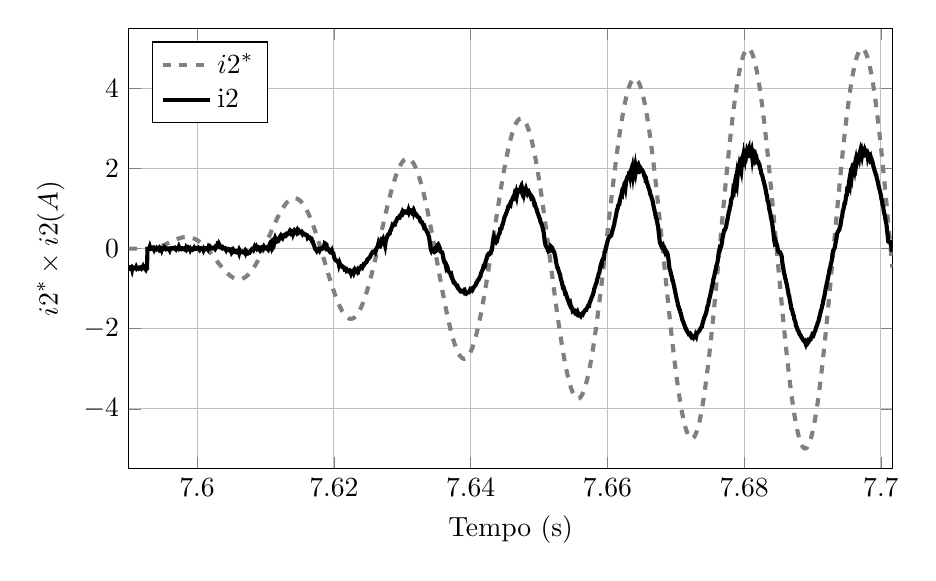
\begin{tikzpicture}

\begin{axis}[%
width=0.8\textwidth,
height=0.461611624834875\textwidth,
scale only axis,
xmin=7.59,
xmax=7.7017,
xtick={ 7.6, 7.62, 7.64, 7.66, 7.68,  7.7},
xlabel={Tempo (s)},
xmajorgrids,
ymin=-5.5,
ymax=5.5,
ytick={-4, -2,  0,  2,  4},
ylabel={$\text{i2}^\text{*}\text{ }\times\text{ i2 (A)}$},
ymajorgrids,
legend style={at={(0.03,0.97)},anchor=north west,draw=black,fill=white,legend cell align=left}
]
\addplot [color=gray,dashed,line width=1.5pt]
  table[row sep=crcr]{7.589999988975	0\\
7.59008332897521	0\\
7.59016666897542	0\\
7.59025000897562	0\\
7.59033331897583	0\\
7.59041665897604	0\\
7.59049999897625	0\\
7.59058333897646	0\\
7.59066667897667	0\\
7.59074998897688	0\\
7.59083332897708	0\\
7.59091666897729	0\\
7.5910000089775	0\\
7.59108331897771	0\\
7.59116665897792	0\\
7.59124999897812	0\\
7.59133333897833	0\\
7.59141667897854	0\\
7.59149998897875	0\\
7.59158332897896	0\\
7.59166666897917	0\\
7.59175000897937	0\\
7.59183331897958	0\\
7.59191665897979	0\\
7.59199999898	0\\
7.59208333898021	0\\
7.59216667898042	0\\
7.59224998898063	0\\
7.59233332898083	0\\
7.59241666898104	0\\
7.59250000898125	0\\
7.59258331898146	0\\
7.59266665898167	0\\
7.59274999898188	0\\
7.59283333898208	0\\
7.59291667898229	-0\\
7.5929999889825	3.92634488473762e-05\\
7.59308332898271	0.000196239747670498\\
7.59316666898292	0.000539330060403448\\
7.59325000898312	0.00111693629130865\\
7.59333331898333	0.00195981918271187\\
7.59341665898354	0.00308594496928202\\
7.59349999898375	0.00450474353583032\\
7.59358333898396	0.00622015616516742\\
7.59366667898417	0.00823262022416316\\
7.59374998898438	0.0105402936125734\\
7.59383332898458	0.0131397849599244\\
7.59391666898479	0.0160265798470743\\
7.594000008985	0.0191952868299359\\
7.59408331898521	0.0226397794705883\\
7.59416665898542	0.0263532796332583\\
7.59424999898563	0.0303284082476884\\
7.59433333898583	0.0345572184241179\\
7.59441667898604	0.0390312192492781\\
7.59449998898625	0.0437413948672979\\
7.59458332898646	0.0486782213623582\\
7.59466666898667	0.0538316828039993\\
7.59475000898687	0.0591912871815809\\
7.59483331898708	0.0647460826087258\\
7.59491665898729	0.0704846739912887\\
7.5949999989875	0.0763952402512923\\
7.59508333898771	0.0824655521447796\\
7.59516667898792	0.0886829906821065\\
7.59524998898813	0.0950345661431947\\
7.59533332898833	0.101506937671426\\
7.59541666898854	0.108086433424836\\
7.59550000898875	0.114759071260276\\
7.59558331898896	0.121510579924313\\
7.59566665898917	0.128326420723332\\
7.59574999898938	0.135191809644302\\
7.59583333898958	0.142091739896904\\
7.59591667898979	0.149011004847002\\
7.59599998899	0.155934221310872\\
7.59608332899021	0.162845853179035\\
7.59616666899042	0.169730235338065\\
7.59625000899062	0.176571597858304\\
7.59633331899083	0.183354090414979\\
7.59641665899104	0.190061806909914\\
7.59649999899125	0.196678810260643\\
7.59658333899146	0.203189157323517\\
7.59666667899167	0.209576923917116\\
7.59674998899188	0.215826229912111\\
7.59683332899208	0.221921264353563\\
7.59691666899229	0.227846310581539\\
7.5970000089925	0.233585771315865\\
7.59708331899271	0.239124193670803\\
7.59716665899292	0.244446294065482\\
7.59724999899313	0.249536982995955\\
7.59733333899333	0.254381389634882\\
7.59741667899354	0.258964886224969\\
7.59749998899375	0.263273112232519\\
7.59758332899396	0.267291998227645\\
7.59766666899417	0.271007789458016\\
7.59775000899438	0.2744070690833\\
7.59783331899458	0.277476781037844\\
7.59791665899479	0.280204252489533\\
7.597999998995	0.282577215863212\\
7.59808333899521	0.284583830397552\\
7.59816667899542	0.286212703204747\\
7.59824998899563	0.287452909803028\\
7.59833332899583	0.288294014092534\\
7.59841666899604	0.288726087745785\\
7.59850000899625	0.28873972898462\\
7.59858331899646	0.288326080716234\\
7.59866665899667	0.287476848001647\\
7.59874999899688	0.286184314830782\\
7.59883333899708	0.284441360179096\\
7.59891667899729	0.282241473321602\\
7.5989999889975	0.279578768380984\\
7.59908332899771	0.276447998087437\\
7.59916666899792	0.272844566728798\\
7.59925000899813	0.268764542270527\\
7.59933331899833	0.264204667626086\\
7.59941665899854	0.259162371059302\\
7.59949999899875	0.253635775701354\\
7.59958333899896	0.247623708166111\\
7.59966667899917	0.241125706248628\\
7.59974998899937	0.234142025692764\\
7.59983332899958	0.226673646015016\\
7.59991666899979	0.218722275372802\\
7.600000009	0.210290354466661\\
7.60008331900021	0.20138105946698\\
7.60016665900042	0.191998303957109\\
7.60024999900063	0.182146739885928\\
7.60033333900083	0.171831757524175\\
7.60041667900104	0.161059484420095\\
7.60049998900125	0.149836783351221\\
7.60058332900146	0.138171249270346\\
7.60066666900167	0.126071205245064\\
7.60075000900188	0.113545697391459\\
7.60083331900208	0.100604488803862\\
7.60091665900229	0.087258052483838\\
7.6009999990025	0.0735175632728483\\
7.60108333900271	0.0593948887943171\\
7.60116667900292	0.0449025794120917\\
7.60124998900312	0.0300538572135612\\
7.60133332900333	0.0148626040269533\\
7.60141666900354	-0.000656651516416185\\
7.60150000900375	-0.0164887478629258\\
7.60158331900396	-0.0326179053472152\\
7.60166665900417	-0.0490277419180695\\
7.60174999900438	-0.0657012897639517\\
7.60183333900458	-0.0826210128213217\\
7.60191667900479	-0.0997688251477116\\
7.601999989005	-0.117126110140371\\
7.60208332900521	-0.134673740580167\\
7.60216666900542	-0.1523920994793\\
7.60225000900563	-0.170261101710329\\
7.60233331900583	-0.188260216392906\\
7.60241665900604	-0.20636849001361\\
7.60249999900625	-0.22456457025323\\
7.60258333900646	-0.242826730494888\\
7.60266667900667	-0.261132894985407\\
7.60274998900687	-0.279460664621447\\
7.60283332900708	-0.297787343330984\\
7.60291666900729	-0.316089965019901\\
7.6030000090075	-0.3343453210526\\
7.60308331900771	-0.352529988234756\\
7.60316665900792	-0.370620357265598\\
7.60324999900813	-0.38859266162636\\
7.60333333900833	-0.406423006870886\\
7.60341667900854	-0.424087400283719\\
7.60349998900875	-0.441561780870407\\
7.60358332900896	-0.458822049644201\\
7.60366666900917	-0.475844100172799\\
7.60375000900938	-0.492603849348319\\
7.60383331900958	-0.509077268343243\\
7.60391665900979	-0.525240413714681\\
7.60399999901	-0.541069458618982\\
7.60408333901021	-0.556540724098386\\
7.60416667901042	-0.571630710401174\\
7.60424998901062	-0.586316128296567\\
7.60433332901083	-0.600573930345441\\
7.60441666901104	-0.614381342087826\\
7.60450000901125	-0.627715893108084\\
7.60458331901146	-0.640555447938618\\
7.60466665901167	-0.652878236763014\\
7.60474999901188	-0.664662885879562\\
7.60483333901208	-0.675888447886246\\
7.60491667901229	-0.686534431548419\\
7.6049999890125	-0.69658083131064\\
7.60508332901271	-0.706008156414354\\
7.60516666901292	-0.714797459583449\\
7.60525000901313	-0.72293036524004\\
7.60533331901333	-0.730389097213255\\
7.60541665901354	-0.737156505904213\\
7.60549999901375	-0.743216094870909\\
7.60558333901396	-0.748552046797211\\
7.60566667901417	-0.753149248810814\\
7.60574998901437	-0.756993317115544\\
7.60583332901458	-0.760070620904149\\
7.60591666901479	-0.762368305518361\\
7.606000009015	-0.76387431482381\\
7.60608331901521	-0.764577412768132\\
7.60616665901542	-0.764467204091479\\
7.60624999901562	-0.763534154159484\\
7.60633333901583	-0.761769607889657\\
7.60641667901604	-0.759165807743159\\
7.60649998901625	-0.755715910754853\\
7.60658332901646	-0.75141400457559\\
7.60666666901667	-0.746255122501714\\
7.60675000901688	-0.740235257467897\\
7.60683331901708	-0.733351374980511\\
7.60691665901729	-0.72560142496992\\
7.6069999990175	-0.716984352541243\\
7.60708333901771	-0.707500107604376\\
7.60716667901792	-0.697149653365293\\
7.60724998901812	-0.685934973661903\\
7.60733332901833	-0.673859079129061\\
7.60741666901854	-0.66092601217862\\
7.60750000901875	-0.647140850781771\\
7.60758331901896	-0.632509711042269\\
7.60766665901917	-0.617039748550505\\
7.60774999901937	-0.600739158509821\\
7.60783333901958	-0.583617174627826\\
7.60791667901979	-0.565684066766932\\
7.60799998902	-0.54695113734975\\
7.60808332902021	-0.527430716516444\\
7.60816666902042	-0.507136156032582\\
7.60825000902063	-0.486081821947517\\
7.60833331902083	-0.464283086004765\\
7.60841665902104	-0.441756315807359\\
7.60849999902125	-0.418518863742611\\
7.60858333902146	-0.394589054672203\\
7.60866667902167	-0.369986172395001\\
7.60874998902187	-0.344730444891467\\
7.60883332902208	-0.318843028360017\\
7.60891666902229	-0.292345990057114\\
7.6090000090225	-0.26526228995439\\
7.60908331902271	-0.237615761227477\\
7.60916665902292	-0.209431089592727\\
7.60924999902312	-0.180733791509366\\
7.60933333902333	-0.151550191266084\\
7.60941667902354	-0.121907396972424\\
7.60949998902375	-0.0918332754767251\\
7.60958332902396	-0.0613564262337166\\
7.60966666902417	-0.0305061541462129\\
7.60975000902438	0.00068755859335144\\
7.60983331902458	0.0321940816345025\\
7.60991665902479	0.0639821665451286\\
7.609999999025	0.0960199778031705\\
7.61008333902521	0.128275124672863\\
7.61016667902542	0.160714693933619\\
7.61024998902562	0.193305283428501\\
7.61033332902583	0.226013036398124\\
7.61041666902604	0.258803676564744\\
7.61050000902625	0.291642543930274\\
7.61058331902646	0.324494631250935\\
7.61066665902667	0.357324621150329\\
7.61074999902687	0.390096923831746\\
7.61083333902708	0.422775715349704\\
7.61091667902729	0.455324976399811\\
7.6109999890275	0.487708531585296\\
7.61108332902771	0.519890089117784\\
7.61116666902792	0.551833280909188\\
7.61125000902813	0.583501703010921\\
7.61133331902833	0.614858956356049\\
7.61141665902854	0.645868687759411\\
7.61149999902875	0.676494631130238\\
7.61158333902896	0.706700648851329\\
7.61166667902917	0.736450773278437\\
7.61174998902938	0.765709248313142\\
7.61183332902958	0.794440571002203\\
7.61191666902979	0.822609533116082\\
7.61200000903	0.850181262659173\\
7.61208331903021	0.877121265264087\\
7.61216665903042	0.903395465422244\\
7.61224999903062	0.928970247503012\\
7.61233333903083	0.953812496513588\\
7.61241667903104	0.977889638551935\\
7.61249998903125	1.00116968090517\\
7.61258332903146	1.023621251746\\
7.61266666903167	1.04521363937994\\
7.61275000903187	1.06591683099659\\
7.61283331903208	1.08570155087809\\
7.61291665903229	1.10453929801893\\
7.6129999990325	1.12240238311105\\
7.61308333903271	1.13926396484921\\
7.61316667903292	1.15509808551185\\
7.61324998903313	1.16987970577333\\
7.61333332903333	1.18358473870417\\
7.61341666903354	1.1961900829166\\
7.61350000903375	1.20767365481334\\
7.61358331903396	1.21801441989854\\
7.61366665903417	1.22719242311065\\
7.61374999903437	1.23518881813763\\
7.61383333903458	1.24198589567634\\
7.61391667903479	1.24756711059847\\
7.613999989035	1.25191710798675\\
7.61408332903521	1.25502174800612\\
7.61416666903542	1.25686812957578\\
7.61425000903562	1.25744461280908\\
7.61433331903583	1.25674084018961\\
7.61441665903604	1.25474775645297\\
7.61449999903625	1.25145762714512\\
7.61458333903646	1.24686405582944\\
7.61466667903667	1.24096199991611\\
7.61474998903688	1.23374778508877\\
7.61483332903708	1.22521911830496\\
7.61491666903729	1.21537509934816\\
7.6150000090375	1.2042162309109\\
7.61508331903771	1.19174442719001\\
7.61516665903792	1.17796302097641\\
7.61524999903812	1.16287676922361\\
7.61533333903833	1.14649185708084\\
7.61541667903854	1.12881590037797\\
7.61549998903875	1.10985794655149\\
7.61558332903896	1.08962847400221\\
7.61566666903917	1.06813938987714\\
7.61575000903937	1.04540402626981\\
7.61583331903958	1.02143713483475\\
7.61591665903979	0.996254879814013\\
7.61599999904	0.969874829474927\\
7.61608333904021	0.942315945960343\\
7.61616667904042	0.9135985735543\\
7.61624998904063	0.883744425367755\\
7.61633332904083	0.852776568450875\\
7.61641666904104	0.820719407340126\\
7.61650000904125	0.787598666050151\\
7.61658331904146	0.753441368522235\\
7.61666665904167	0.718275817542871\\
7.61674999904188	0.682131572147739\\
7.61683333904208	0.645039423528115\\
7.61691667904229	0.60703136945848\\
7.6169999890425	0.568140587265829\\
7.61708332904271	0.528401405362841\\
7.61716666904292	0.487849273368815\\
7.61725000904312	0.446520730843884\\
7.61733331904333	0.404453374663717\\
7.61741665904354	0.361685825063497\\
7.61749999904375	0.318257690381593\\
7.61758333904396	0.274209530534895\\
7.61766667904417	0.22958281925932\\
7.61774998904438	0.184419905150532\\
7.61783332904458	0.138763971541359\\
7.61791666904479	0.0926589952538724\\
7.618000009045	0.0461497042654726\\
7.61808331904521	-0.00071846567028672\\
7.61816665904542	-0.0478994154060793\\
7.61824999904563	-0.0953464277430423\\
7.61833333904583	-0.143012213688272\\
7.61841667904604	-0.190848959581775\\
7.61849998904625	-0.238808375045917\\
7.61858332904646	-0.286841741709292\\
7.61866666904667	-0.334899962655878\\
7.61875000904687	-0.382933612549322\\
7.61883331904708	-0.430892988381248\\
7.61891665904729	-0.478728160791543\\
7.6189999990475	-0.526389025907753\\
7.61908333904771	-0.573825357649884\\
7.61916667904792	-0.62098686044618\\
7.61924998904813	-0.667823222304736\\
7.61933332904833	-0.714284168185186\\
7.61941666904854	-0.760319513614124\\
7.61950000904875	-0.805879218487395\\
7.61958331904896	-0.850913441001943\\
7.61966665904917	-0.8953725916595\\
7.61974999904938	-0.939207387284068\\
7.61983333904958	-0.98236890499488\\
7.61991667904979	-1.0248086360763\\
7.61999998905	-1.06647853968599\\
7.62008332905021	-1.10733109634257\\
7.62016666905042	-1.147319361134\\
7.62025000905062	-1.18639701658797\\
7.62033331905083	-1.22451842514555\\
7.62041665905104	-1.26163868117986\\
7.62049999905125	-1.29771366250125\\
7.62058333905146	-1.33270008129135\\
7.62066667905167	-1.3665555344082\\
7.62074998905188	-1.39923855300549\\
7.62083332905208	-1.43070865140917\\
7.62091666905229	-1.46092637519543\\
7.6210000090525	-1.48985334841445\\
7.62108331905271	-1.51745231990535\\
7.62116665905292	-1.5436872086481\\
7.62124999905313	-1.56852314809924\\
7.62133333905333	-1.59192652945908\\
7.62141667905354	-1.61386504381887\\
7.62149998905375	-1.63430772313746\\
7.62158332905396	-1.65322497999823\\
7.62166666905417	-1.6705886460977\\
7.62175000905437	-1.68637200941885\\
7.62183331905458	-1.70054985004323\\
7.62191665905479	-1.71309847455705\\
7.621999999055	-1.72399574900805\\
7.62208333905521	-1.73322113037105\\
7.62216667905542	-1.74075569648178\\
7.62224998905563	-1.74658217439974\\
7.62233332905583	-1.75068496716269\\
7.62241666905604	-1.75305017889671\\
7.62250000905625	-1.75366563824742\\
7.62258331905646	-1.75252092009981\\
7.62266665905667	-1.74960736555541\\
7.62274999905688	-1.74491810013781\\
7.62283333905708	-1.73844805019876\\
7.62291667905729	-1.7301939574994\\
7.6229999890575	-1.72015439194256\\
7.62308332905771	-1.70832976243439\\
7.62316666905792	-1.69472232585508\\
7.62325000905813	-1.67933619412073\\
7.62333331905833	-1.66217733932009\\
7.62341665905854	-1.64325359691213\\
7.62349999905875	-1.62257466697231\\
7.62358333905896	-1.60015211347731\\
7.62366667905917	-1.57599936162045\\
7.62374998905938	-1.55013169315158\\
7.62383332905958	-1.5225662397377\\
7.62391666905979	-1.49332197434252\\
7.62400000906	-1.46241970062522\\
7.62408331906021	-1.42988204036099\\
7.62416665906042	-1.39573341888773\\
7.62424999906063	-1.36000004858576\\
7.62433333906083	-1.32270991039935\\
7.62441667906104	-1.28389273341087\\
7.62449998906125	-1.24357997248078\\
7.62458332906146	-1.20180478396858\\
7.62466666906167	-1.158601999552\\
7.62475000906188	-1.11400809816381\\
7.62483331906208	-1.06806117606772\\
7.62491665906229	-1.02080091509696\\
7.6249999990625	-0.97226854908098\\
7.62508333906271	-0.922506828488123\\
7.62516667906292	-0.871559983313621\\
7.62524998906312	-0.81947368424476\\
7.62533332906333	-0.766295002136659\\
7.62541666906354	-0.712072365834217\\
7.62550000906375	-0.656855518377615\\
7.62558331906396	-0.600695471630656\\
7.62566665906417	-0.543644459373046\\
7.62574999906438	-0.485755888899518\\
7.62583333906458	-0.427084291170461\\
7.62591667906479	-0.367685269560426\\
7.625999989065	-0.307615447252558\\
7.62608332906521	-0.246932413328641\\
7.62616666906542	-0.185694667605994\\
7.62625000906563	-0.123961564274029\\
7.62633331906583	-0.0617932543847333\\
7.62641665906604	0.000749372747221162\\
7.62649999906625	0.0636047491776554\\
7.62658333906646	0.126710688940956\\
7.62666667906667	0.190004449573373\\
7.62674998906687	0.253422794490687\\
7.62683332906708	0.316902056158215\\
7.62691666906729	0.380378199990083\\
7.6270000090675	0.443786888913631\\
7.62708331906771	0.507063548533901\\
7.62716665906792	0.570143432832223\\
7.62724999906813	0.632961690332152\\
7.62733333906833	0.695453430665178\\
7.62741667906854	0.757553791468022\\
7.62749998906875	0.819198005542657\\
7.62758332906896	0.880321468209662\\
7.62766666906917	0.940859804785077\\
7.62775000906938	1.00074893811046\\
7.62783331906958	1.0599251560656\\
7.62791665906979	1.11832517899297\\
7.62799999907	1.17588622696295\\
7.62808333907021	1.23254608680873\\
7.62816667907042	1.28824317885953\\
7.62824998907062	1.34291662330128\\
7.62833332907083	1.39650630609355\\
7.62841666907104	1.448952944372\\
7.62850000907125	1.5001981512658\\
7.62858331907146	1.55018450005985\\
7.62866665907167	1.59885558763193\\
7.62874999907188	1.64615609709563\\
7.62883333907208	1.69203185958026\\
7.62891667907229	1.73642991507968\\
7.6289999890725	1.77929857230281\\
7.62908332907271	1.82058746745904\\
7.62916666907292	1.86024762191318\\
7.62925000907313	1.89823149864486\\
7.62933331907333	1.93449305744895\\
7.62941665907354	1.96898780881411\\
7.62949999907375	2.00167286641811\\
7.62958333907396	2.03250699817956\\
7.62966667907417	2.06145067580712\\
7.62974998907437	2.08846612278852\\
7.62983332907458	2.11351736076307\\
7.62991666907479	2.13657025422315\\
7.630000009075	2.15759255349124\\
7.63008331907521	2.17655393592111\\
7.63016665907542	2.19342604527313\\
7.63024999907563	2.20818252921557\\
7.63033333907583	2.22079907490545\\
7.63041667907604	2.23125344260447\\
7.63049998907625	2.23952549728721\\
7.63058332907646	2.245597238201\\
7.63066666907667	2.24945282633864\\
7.63075000907688	2.25107860978729\\
7.63083331907708	2.25046314691906\\
7.63091665907729	2.24759722739054\\
7.6309999990775	2.24247389092122\\
7.63108333907771	2.23508844382265\\
7.63116667907792	2.22543847325241\\
7.63124998907812	2.21352385916936\\
7.63133332907833	2.19934678396902\\
7.63141666907854	2.18291173978001\\
7.63150000907875	2.1642255334052\\
7.63158331907896	2.1432972888933\\
7.63166665907917	2.12013844772928\\
7.63174999907937	2.09476276663426\\
7.63183333907958	2.06718631296821\\
7.63191667907979	2.037427457731\\
7.63199998908	2.00550686616005\\
7.63208332908021	1.97144748592518\\
7.63216666908042	1.93527453292391\\
7.63225000908063	1.89701547468283\\
7.63233331908083	1.85670001137331\\
7.63241665908104	1.81436005445219\\
7.63249999908125	1.77002970294071\\
7.63258333908146	1.72374521735751\\
7.63266667908167	1.67554499132378\\
7.63274998908187	1.6254695208614\\
7.63283332908208	1.57356137140726\\
7.63291666908229	1.51986514256941\\
7.6330000090825	1.46442743065313\\
7.63308331908271	1.4072967889875\\
7.63316665908292	1.3485236860853\\
7.63324999908312	1.28816046167168\\
7.63333333908333	1.22626128061909\\
7.63341667908354	1.16288208482851\\
7.63349998908375	1.09808054309913\\
7.63358332908396	1.03191599903104\\
7.63366666908417	0.964449417007492\\
7.63375000908438	0.895743326305595\\
7.63383331908458	0.825861763386417\\
7.63391665908479	0.75487021241743\\
7.633999999085	0.682835544082377\\
7.63408333908521	0.609825952735541\\
7.63416667908542	0.535910891959331\\
7.63424998908562	0.461161008585957\\
7.63433332908583	0.385648075245797\\
7.63441666908604	0.309444921506751\\
7.63450000908625	0.23262536367063\\
7.63458331908646	0.155264133294187\\
7.63466665908667	0.0774368045039944\\
7.63474999908687	-0.000780279824155447\\
7.63483333908708	-0.0793100829492315\\
7.63491667908729	-0.158074950138869\\
7.6349999890875	-0.236996685458474\\
7.63508332908771	-0.315996629399599\\
7.63516666908792	-0.394995737270514\\
7.63525000908813	-0.473914658270874\\
7.63533331908833	-0.552673815171386\\
7.63541665908854	-0.63119348451848\\
7.63549999908875	-0.709393877283199\\
7.63558333908896	-0.787195219872761\\
7.63566667908917	-0.864517835422604\\
7.63574998908938	-0.941282225286163\\
7.63583332908958	-1.01740915063914\\
7.63591666908979	-1.09281971411459\\
7.63600000909	-1.16743544138497\\
7.63608331909021	-1.24117836260681\\
7.63616665909042	-1.31397109364381\\
7.63624999909062	-1.38573691698399\\
7.63633333909083	-1.45639986226641\\
7.63641667909104	-1.52588478633339\\
7.63649998909125	-1.59411745272417\\
7.63658332909146	-1.66102461052625\\
7.63666666909167	-1.7265340725011\\
7.63675000909188	-1.79057479240143\\
7.63683331909208	-1.85307694139761\\
7.63691665909229	-1.91397198353174\\
7.6369999990925	-1.97319275011831\\
7.63708333909271	-2.03067351301141\\
7.63716667909292	-2.08635005665927\\
7.63724998909313	-2.14015974886803\\
7.63733332909333	-2.19204161019743\\
7.63741666909354	-2.2419363819126\\
7.63750000909375	-2.28978659241719\\
7.63758331909396	-2.3355366220943\\
7.63766665909417	-2.37913276648346\\
7.63774999909437	-2.42052329772288\\
7.63783333909458	-2.45965852418812\\
7.63791667909479	-2.49649084825988\\
7.637999989095	-2.53097482215517\\
7.63808332909521	-2.56306720175818\\
7.63816666909542	-2.59272699838869\\
7.63825000909562	-2.61991552844807\\
7.63833331909583	-2.64459646088478\\
7.63841665909604	-2.66673586242337\\
7.63849999909625	-2.68630224050303\\
7.63858333909646	-2.70326658387408\\
7.63866667909667	-2.71760240080286\\
7.63874998909688	-2.7292857548379\\
7.63883332909708	-2.73829529809266\\
7.63891666909729	-2.74461230200228\\
7.6390000090975	-2.74822068551459\\
7.63908331909771	-2.74910704067789\\
7.63916665909792	-2.74726065559071\\
7.63924999909812	-2.74267353468127\\
7.63933333909833	-2.73534041628703\\
7.63941667909854	-2.7252587875075\\
7.63949998909875	-2.71242889630606\\
7.63958332909896	-2.69685376083933\\
7.63966666909917	-2.67853917599548\\
7.63975000909937	-2.65749371712563\\
7.63983331909958	-2.63372874095532\\
7.63991665909979	-2.60725838366588\\
7.6399999991	-2.57809955613847\\
7.64008333910021	-2.54627193635638\\
7.64016667910042	-2.51179795896412\\
7.64024998910063	-2.47470280198471\\
7.64033332910083	-2.43501437069967\\
7.64041666910104	-2.39276327869879\\
7.64050000910125	-2.34798282611012\\
7.64058331910146	-2.30070897502315\\
7.64066665910167	-2.2509803221214\\
7.64074999910187	-2.19883806854338\\
7.64083333910208	-2.1443259869937\\
7.64091667910229	-2.08749038612927\\
7.6409999891025	-2.02838007224821\\
7.64108332910271	-1.96704630831193\\
7.64116666910292	-1.90354277033374\\
7.64125000910312	-1.83792550117024\\
7.64133331910333	-1.77025286175427\\
7.64141665910354	-1.70058547981119\\
7.64149999910375	-1.62898619610288\\
7.64158333910396	-1.5555200082464\\
7.64166667910417	-1.48025401215721\\
7.64174998910438	-1.4032573411689\\
7.64183332910458	-1.32460110288464\\
7.64191666910479	-1.24435831381733\\
7.642000009105	-1.16260383187833\\
7.64208331910521	-1.07941428677698\\
7.64216665910542	-0.994868008395221\\
7.64224999910563	-0.909044953204205\\
7.64233333910583	-0.822026628791709\\
7.64241667910604	-0.733896016571566\\
7.64249998910625	-0.644737492748202\\
7.64258332910646	-0.554636747611491\\
7.64266666910667	-0.463680703239037\\
7.64275000910687	-0.371957429684862\\
7.64283331910708	-0.279556059735267\\
7.64291665910729	-0.186566702314345\\
7.6429999991075	-0.0930803546232569\\
7.64308333910771	0.000811186901088293\\
7.64316667910792	0.0950154167208063\\
7.64324998910813	0.189439211336781\\
7.64333332910833	0.283988921343574\\
7.64341666910854	0.37857046430851\\
7.64350000910875	0.473089418382811\\
7.64358331910896	0.567451116551665\\
7.64366665910917	0.66156074142914\\
7.64374999910938	0.755323420503059\\
7.64383333910958	0.848644321734175\\
7.64391667910979	0.94142874941337\\
7.64399998911	1.03358224018003\\
7.64408332911021	1.1250106591043\\
7.64416666911042	1.21562029573561\\
7.64425000911062	1.30531796001952\\
7.64433331911083	1.39401107798486\\
7.64441665911104	1.48160778710315\\
7.64449999911125	1.56801703122203\\
7.64458333911146	1.65314865497502\\
7.64466667911167	1.73691349756986\\
7.64474998911188	1.81922348585805\\
7.64483332911208	1.89999172658882\\
7.64491666911229	1.97913259775123\\
7.6450000091125	2.05656183890867\\
7.64508331911271	2.13219664043086\\
7.64516665911292	2.20595573152941\\
7.64524999911313	2.27775946700363\\
7.64533333911333	2.3475299126047\\
7.64541667911354	2.41519092892718\\
7.64549998911375	2.48066825373828\\
7.64558332911396	2.54388958265637\\
7.64566666911417	2.60478464809205\\
7.64575000911437	2.66328529636617\\
7.64583331911458	2.7193255629212\\
7.64591665911479	2.77284174554374\\
7.645999999115	2.82377247551798\\
7.64608333911521	2.87205878663165\\
7.64616667911542	2.91764418195814\\
7.64624998911563	2.9604746983402\\
7.64633332911583	3.00049896850322\\
7.64641666911604	3.03766828072785\\
7.64650000911625	3.07193663601431\\
7.64658331911646	3.10326080267299\\
7.64666665911667	3.13160036827832\\
7.64674999911688	3.15691778892563\\
7.64683333911708	3.17917843573294\\
7.64691667911729	3.19835063853261\\
7.6469999891175	3.21440572670027\\
7.64708332911771	3.22731806707133\\
7.64716666911792	3.23706509889811\\
7.64725000911813	3.24362736580356\\
7.64733331911833	3.24698854469054\\
7.64741665911854	3.24713547156848\\
7.64749999911875	3.24405816426236\\
7.64758333911896	3.23774984197201\\
7.64766667911917	3.22820694165284\\
7.64774998911938	3.21542913119235\\
7.64783332911958	3.19941931935972\\
7.64791666911979	3.1801836625093\\
7.64800000912	3.15773156802194\\
7.64808331912021	3.13207569447126\\
7.64816665912042	3.10323194850545\\
7.64824999912063	3.07121947843846\\
7.64833333912083	3.03606066454767\\
7.64841667912104	2.99778110607852\\
7.64849998912125	2.95640960496003\\
7.64858332912146	2.91197814623841\\
7.64866666912167	2.86452187523928\\
7.64875000912188	2.81407907147241\\
7.64883331912208	2.76069111929634\\
7.64891665912229	2.70440247536347\\
7.6489999991225	2.6452606328695\\
7.64908333912271	2.58331608263458\\
7.64916667912292	2.51862227104669\\
7.64924998912312	2.45123555490103\\
7.64933332912333	2.38121515317265\\
7.64941666912354	2.30862309576247\\
7.64950000912375	2.23352416926023\\
7.64958331912396	2.15598585977108\\
7.64966665912417	2.07607829285541\\
7.64974999912438	1.99387417063488\\
7.64983333912458	1.90944870612046\\
7.64991667912479	1.82287955482113\\
7.649999989125	1.73424674369532\\
7.65008332912521	1.64363259750929\\
7.65016666912542	1.55112166267015\\
7.65025000912563	1.45680062860361\\
7.65033331912583	1.36075824674916\\
7.65041665912604	1.26308524724836\\
7.65049999912625	1.16387425340403\\
7.65058333912646	1.06321969399098\\
7.65066667912667	0.961217713501042\\
7.65074998912687	0.857966080407591\\
7.65083332912708	0.753564093537073\\
7.65091666912729	0.648112486637025\\
7.6510000091275	0.541713331232278\\
7.65108331912771	0.434469937862974\\
7.65116665912792	0.326486755799904\\
7.65124999912813	0.217869271334504\\
7.65133333912833	0.108723904742519\\
7.65141667912854	-0.000842093978021569\\
7.65149998912875	-0.110720750492382\\
7.65158332912896	-0.220803472534694\\
7.65166666912917	-0.330981157228675\\
7.65175000912938	-0.441144299217422\\
7.65183331912958	-0.55118309949511\\
7.65191665912979	-0.660987574832456\\
7.65199999913	-0.770447667686895\\
7.65208333913021	-0.879453356487639\\
7.65216667913042	-0.987894766185152\\
7.65224998913062	-1.09566227895398\\
7.65233332913083	-1.20264664493746\\
7.65241666913104	-1.30873909292244\\
7.65250000913125	-1.41383144083209\\
7.65258331913146	-1.51781620592445\\
7.65266665913167	-1.62058671458476\\
7.65274999913188	-1.7220372115995\\
7.65283333913208	-1.82206296880024\\
7.65291667913229	-1.92056039296605\\
7.6529999891325	-2.01742713287332\\
7.65308332913271	-2.11256218538272\\
7.65316666913292	-2.20586600045347\\
7.65325000913313	-2.29724058497621\\
7.65333331913333	-2.38658960531623\\
7.65341665913354	-2.4738184884603\\
7.65349999913375	-2.55883452166122\\
7.65358333913396	-2.64154695047553\\
7.65366667913417	-2.72186707509109\\
7.65374998913437	-2.79970834484297\\
7.65383332913458	-2.8749864508173\\
7.65391666913479	-2.94761941644472\\
7.654000009135	-3.01752768598667\\
7.65408331913521	-3.08463421081973\\
7.65416665913542	-3.14886453342521\\
7.65424999913563	-3.21014686899319\\
7.65433333913583	-3.2684121845525\\
7.65441667913604	-3.32359427554043\\
7.65449998913625	-3.37562983972816\\
7.65458332913646	-3.42445854842053\\
7.65466666913667	-3.47002311485127\\
7.65475000913688	-3.51226935969752\\
7.65483331913708	-3.55114627363994\\
7.65491665913729	-3.58660607689791\\
7.6549999991375	-3.61860427567187\\
7.65508333913771	-3.6470997154279\\
7.65516667913792	-3.67205463096285\\
7.65524998913812	-3.69343469319113\\
7.65533332913833	-3.71120905259768\\
7.65541666913854	-3.72535037930476\\
7.65550000913875	-3.73583489970356\\
7.65558331913896	-3.74264242960483\\
7.65566665913917	-3.74575640386649\\
7.65574999913937	-3.74516390245908\\
7.65583333913958	-3.74085567293402\\
7.65591667913979	-3.73282614926275\\
7.65599998914	-3.72107346701866\\
7.65608332914021	-3.70559947487721\\
7.65616666914042	-3.68640974241337\\
7.65625000914063	-3.66351356417927\\
7.65633331914083	-3.63692396004841\\
7.65641665914104	-3.60665767181689\\
7.65649999914125	-3.57273515605557\\
7.65658333914146	-3.53518057321105\\
7.65666667914167	-3.49402177295687\\
7.65674998914187	-3.44929027580065\\
7.65683332914208	-3.40102125095594\\
7.65691666914229	-3.34925349049212\\
7.6570000091425	-3.2940293797789\\
7.65708331914271	-3.23539486424602\\
7.65716665914292	-3.17339941248255\\
7.65724999914312	-3.10809597570379\\
7.65733333914333	-3.03954094361759\\
7.65741667914354	-2.96779409672579\\
7.65749998914375	-2.89291855509968\\
7.65758332914396	-2.81498072367279\\
7.65766666914417	-2.73405023409709\\
7.65775000914438	-2.650199883213\\
7.65783331914458	-2.56350556818672\\
7.65791665914479	-2.47404621837191\\
7.657999999145	-2.38190372395654\\
7.65808333914521	-2.28716286145858\\
7.65816667914542	-2.18991121613804\\
7.65824998914562	-2.09023910139586\\
7.65833332914583	-1.98823947523344\\
7.65841666914604	-1.88400785384968\\
7.65850000914625	-1.77764222245567\\
7.65858331914646	-1.6692429433899\\
7.65866665914667	-1.55891266162\\
7.65874999914687	-1.44675620771974\\
7.65883333914708	-1.33288049841283\\
7.65891667914729	-1.21739443477776\\
7.6589999891475	-1.10040879821038\\
7.65908332914771	-0.982036144243618\\
7.65916666914792	-0.862390694325946\\
7.65925000914813	-0.74158822566256\\
7.65933331914833	-0.61974595922552\\
7.65941665914854	-0.496982446041087\\
7.65949999914875	-0.373417451864542\\
7.65958333914896	-0.249171840354664\\
7.65966667914917	-0.124367454861782\\
7.65974998914937	0.000873001054954144\\
7.65983332914958	0.126426084263956\\
7.65991666914979	0.252167733732606\\
7.66000000915	0.377973393113776\\
7.66008331915021	0.503718134126334\\
7.66016665915042	0.629276780607408\\
7.66024999915062	0.754524033113248\\
7.66033333915083	0.87933459394465\\
7.66041667915104	1.00358329247222\\
7.66049998915125	1.12714521063613\\
7.66058332915146	1.24989580849459\\
7.66066666915167	1.37171104969489\\
7.66075000915188	1.49246752674059\\
7.66083331915208	1.61204258592857\\
7.66091665915229	1.73031445182938\\
7.6609999991525	1.84716235118466\\
7.66108333915271	1.96246663609584\\
7.66116667915292	2.07610890637845\\
7.66124998915313	2.18797213095708\\
7.66133332915333	2.29794076817678\\
7.66141666915354	2.40590088490738\\
7.66150000915375	2.51174027431812\\
7.66158331915396	2.61534857220119\\
7.66166665915417	2.71661737172379\\
7.66174999915437	2.81544033648973\\
7.66183333915458	2.91171331179303\\
7.66191667915479	3.00533443394742\\
7.661999989155	3.09620423757748\\
7.66208332915521	3.18422576075875\\
7.66216666915542	3.26930464789632\\
7.66225000915562	3.35134925023307\\
7.66233331915583	3.43027072388129\\
7.66241665915604	3.5059831252733\\
7.66249999915625	3.57840350392923\\
7.66258333915646	3.64745199244263\\
7.66266667915667	3.71305189358702\\
7.66274998915688	3.77512976444921\\
7.66283332915708	3.83361549749819\\
7.66291666915729	3.88844239850086\\
7.6630000091575	3.93954726119932\\
7.66308331915771	3.98687043866719\\
7.66316665915792	4.03035591126556\\
7.66324999915812	4.06995135112284\\
7.66333333915833	4.10560818306542\\
7.66341667915854	4.13728164193017\\
7.66349998915875	4.16493082619276\\
7.66358332915896	4.18851874784966\\
7.66366666915917	4.2080123784951\\
7.66375000915937	4.2233826915382\\
7.66383331915958	4.23460470050901\\
7.66391665915979	4.24165749340612\\
7.66399999916	4.24452426304246\\
7.66408333916021	4.24319233334969\\
7.66416667916042	4.23765318160568\\
7.66424998916063	4.22790245655349\\
7.66433332916083	4.21393999238448\\
7.66441666916104	4.19576981856207\\
7.66450000916125	4.17340016546704\\
7.66458331916146	4.14684346584926\\
7.66466665916167	4.11611635207489\\
7.66474999916187	4.08123964916252\\
7.66483333916208	4.04223836360571\\
7.66491667916229	3.99914166798364\\
7.6649999891625	3.95198288136608\\
7.66508332916271	3.90079944552279\\
7.66516666916292	3.84563289695186\\
7.66525000916312	3.78652883474583\\
7.66533331916333	3.72353688431852\\
7.66541665916354	3.65671065701964\\
7.66549999916375	3.58610770566878\\
7.66558333916396	3.51178947604411\\
7.66566667916417	3.4338212543657\\
7.66574998916438	3.35227211081699\\
7.66583332916458	3.26721483915268\\
7.66591666916479	3.17872589244455\\
7.666000009165	3.08688531502153\\
7.66608331916521	2.99177667066354\\
7.66616665916542	2.89348696711321\\
7.66624999916563	2.79210657697275\\
7.66633333916583	2.68772915505769\\
7.66641667916604	2.58045155228228\\
7.66649998916625	2.47037372615562\\
7.66658332916646	2.35759864797059\\
7.66666666916667	2.24223220677156\\
7.66675000916687	2.12438311019007\\
7.66683331916708	2.00416278224119\\
7.66691665916729	1.88168525817619\\
7.6669999991675	1.75706707649084\\
7.66708333916771	1.63042716819112\\
7.66716667916792	1.50188674342164\\
7.66724998916813	1.37156917556454\\
7.66733332916833	1.23959988291971\\
7.66741666916854	1.10610620807965\\
7.66750000916875	0.97121729511482\\
7.66758331916896	0.835063964688096\\
7.66766665916917	0.697778587218763\\
7.66774999916938	0.5594949542192\\
7.66783333916958	0.420348147929181\\
7.66791667916979	0.280474409374824\\
7.66799998917	0.140011004981045\\
7.66808332917021	-0.000903908131886802\\
7.66816666917042	-0.142131418035531\\
7.66825000917062	-0.283531994930519\\
7.66833331917083	-0.424965628998877\\
7.66841665917104	-0.566291969035246\\
7.66849999917125	-0.707370461719707\\
7.66858333917146	-0.848060491394041\\
7.66866667917167	-0.988221520202407\\
7.66874998917188	-1.1277132284568\\
7.66883332917208	-1.26639565508711\\
7.66891666917229	-1.40412933803521\\
7.6690000091725	-1.54077545445232\\
7.66908331917271	-1.67619596055873\\
7.66916665917292	-1.81025373102506\\
7.66924999917313	-1.94281269773431\\
7.66933333917333	-2.07373798778456\\
7.66941667917354	-2.20289606059219\\
7.66949998917375	-2.33015484395667\\
7.66958332917396	-2.45538386894811\\
7.66966666917417	-2.57845440348025\\
7.66975000917437	-2.69923958443205\\
7.66983331917458	-2.81761454818278\\
7.66991665917479	-2.93345655942618\\
7.669999999175	-3.04664513813136\\
7.67008333917521	-3.15706218451917\\
7.67016667917542	-3.26459210192485\\
7.67024998917563	-3.36912191741932\\
7.67033332917583	-3.47054140006387\\
7.67041666917604	-3.56874317667454\\
7.67050000917625	-3.66362284497534\\
7.67058331917646	-3.75507908402142\\
7.67066665917667	-3.84301376177592\\
7.67074999917688	-3.92733203972687\\
7.67083333917708	-4.00794247443326\\
7.67091667917729	-4.08475711589209\\
7.6709999891775	-4.15769160262154\\
7.67108332917771	-4.22666525335799\\
7.67116666917792	-4.29160115526822\\
7.67125000917812	-4.35242624858119\\
7.67133331917833	-4.40907140754739\\
7.67141665917854	-4.46147151763687\\
7.67149999917875	-4.5095655488912\\
7.67158333917896	-4.55329662534777\\
7.67166667917917	-4.59261209045897\\
7.67174998917938	-4.62746356843244\\
7.67183332917958	-4.65780702142268\\
7.67191666917979	-4.68360280250819\\
7.67200000918	-4.70481570439252\\
7.67208331918021	-4.72141500377165\\
7.67216665918042	-4.73337450131447\\
7.67224999918063	-4.74067255720741\\
7.67233333918083	-4.74329212221842\\
7.67241667918104	-4.7412207642403\\
7.67249998918125	-4.73445069027734\\
7.67258332918146	-4.72297876384424\\
7.67266666918167	-4.70680651775031\\
7.67275000918188	-4.68594016224693\\
7.67283331918208	-4.66039058852071\\
7.67291665918229	-4.63017336751924\\
7.6729999991825	-4.59530874410136\\
7.67308333918271	-4.55582162650816\\
7.67316667918292	-4.51174157115585\\
7.67324998918313	-4.46310276275623\\
7.67333332918333	-4.40994398977529\\
7.67341666918354	-4.35230861524493\\
7.67350000918375	-4.29024454294778\\
7.67358331918396	-4.22380417899955\\
7.67366665918417	-4.15304438885815\\
7.67374999918438	-4.07802644979327\\
7.67383333918458	-3.998815998855\\
7.67391667918479	-3.91548297638444\\
7.673999989185	-3.8281015651138\\
7.67408332918521	-3.7367501249082\\
7.67416666918542	-3.64151112320568\\
7.67425000918563	-3.54247106121632\\
7.67433331918583	-3.43972039594597\\
7.67441665918604	-3.33335345811409\\
7.67449999918625	-3.22346836603971\\
7.67458333918646	-3.1101669355736\\
7.67466667918667	-2.99355458615883\\
7.67474998918687	-2.87374024310598\\
7.67483332918708	-2.75083623617321\\
7.67491666918729	-2.62495819454533\\
7.6750000091875	-2.49622493830968\\
7.67508331918771	-2.36475836653047\\
7.67516665918792	-2.23068334202671\\
7.67524999918813	-2.09412757296248\\
7.67533333918833	-1.95522149136168\\
7.67541667918854	-1.81409812866251\\
7.67549998918875	-1.67089298843045\\
7.67558332918896	-1.52574391635132\\
7.67566666918917	-1.37879096762905\\
7.67575000918938	-1.23017627191568\\
7.67583331918958	-1.08004389590369\\
7.67591665918979	-0.928539703713632\\
7.67599999919	-0.775811215212005\\
7.67608333919021	-0.622007462397313\\
7.67616667919042	-0.467278843993819\\
7.67624998919062	-0.311776978394983\\
7.67633332919083	-0.155693818549155\\
7.67641666919104	0.000738575461149846\\
7.67650000919125	0.157297421746704\\
7.67658331919146	0.313779319837124\\
7.67666665919167	0.469998045701268\\
7.67674999919188	0.625779858974878\\
7.67683333919208	0.780959399296177\\
7.67691667919229	0.935376793509667\\
7.6769999891925	1.088875826236\\
7.67708332919271	1.24130287082881\\
7.67716666919292	1.39250631457816\\
7.67725000919313	1.54233628772875\\
7.67733331919333	1.69064457237981\\
7.67741665919354	1.83728461490629\\
7.67749999919375	1.98211159648828\\
7.67758333919396	2.12498253539156\\
7.67766667919417	2.26575640596034\\
7.67774998919437	2.40429426583926\\
7.67783332919458	2.54045938666759\\
7.67791666919479	2.67411738557679\\
7.678000009195	2.80513635597971\\
7.67808331919521	2.93338699677514\\
7.67816665919542	3.05874273943871\\
7.67824999919563	3.18107987265988\\
7.67833333919583	3.30027766428763\\
7.67841667919604	3.41621848040383\\
7.67849998919625	3.52878790137455\\
7.67858332919646	3.63787483474803\\
7.67866666919667	3.74337162487884\\
7.67875000919688	3.84517415916549\\
7.67883331919708	3.94318197079408\\
7.67891665919729	4.03729833788546\\
7.6789999991975	4.12743037894721\\
7.67908333919771	4.21348914453614\\
7.67916667919792	4.29538970504037\\
7.67924998919812	4.37305123449453\\
7.67933332919833	4.44639709034519\\
7.67941666919854	4.51535488908774\\
7.67950000919875	4.57985657770017\\
7.67958331919896	4.63983850080321\\
7.67966665919917	4.69524146348046\\
7.67974999919938	4.74601078969662\\
7.67983333919958	4.79209637625618\\
7.67991667919979	4.83345274224918\\
7.6799999892	4.87003907393541\\
7.68008332920021	4.9018192650226\\
7.68016666920042	4.92876195229903\\
7.68025000920063	4.95084054658518\\
7.68033331920083	4.96803325897407\\
7.68041665920104	4.98032312233428\\
7.68049999920125	4.98769800805444\\
7.68058333920146	4.99015063801273\\
7.68066667920167	4.9876785917595\\
7.68074998920187	4.98028430890592\\
7.68083332920208	4.96797508671647\\
7.68091666920229	4.95076307290733\\
7.6810000092025	4.92866525365811\\
7.68108331920271	4.90170343684848\\
7.68116665920292	4.86990423053652\\
7.68124999920312	4.83329901669968\\
7.68133333920333	4.79192392026462\\
7.68141667920354	4.74581977345624\\
7.68149998920375	4.69503207550123\\
7.68158332920396	4.63961094772579\\
7.68166666920417	4.57961108409196\\
7.68175000920438	4.51509169722128\\
7.68183331920458	4.44611645995907\\
7.68191665920479	4.37275344253702\\
7.681999999205	4.29507504539612\\
7.68208333920521	4.2131579277361\\
7.68216667920542	4.12708293186212\\
7.68224998920562	4.03693500340316\\
7.68233332920583	3.94280310748091\\
7.68241666920604	3.84478014091196\\
7.68250000920625	3.74296284052987\\
7.68258331920646	3.63745168771755\\
7.68266665920667	3.52835080924432\\
7.68274999920687	3.41576787450532\\
7.68283333920708	3.29981398926484\\
7.68291667920729	3.18060358600832\\
7.6829999892075	3.05825431101134\\
7.68308332920771	2.9328869082369\\
7.68316666920792	2.80462510017577\\
7.68325000920813	2.67359546574725\\
7.68333331920833	2.53992731538114\\
7.68341665920854	2.40375256340388\\
7.68349999920875	2.26520559785511\\
7.68358333920896	2.12442314786284\\
7.68366667920917	1.98154414870834\\
7.68374998920937	1.83670960471379\\
7.68383332920958	1.69006245008803\\
7.68391666920979	1.54174740786775\\
7.68400000921	1.39191084709332\\
7.68408331921021	1.24070063836024\\
7.68416665921042	1.0882660078887\\
7.68424999921062	0.934757390255326\\
7.68433333921083	0.780326279932395\\
7.68441667921104	0.625125081781105\\
7.68449998921125	0.469306960646363\\
7.68458332921146	0.313025690201579\\
7.68466666921167	0.156435501192615\\
7.68475000921188	-0.000309070769339045\\
7.68483331921208	-0.157053337715758\\
7.68491665921229	-0.313642611979131\\
7.6849999992125	-0.469922358851012\\
7.68508333921271	-0.625738349089121\\
7.68516667921292	-0.780936811122986\\
7.68524998921313	-0.935364582807916\\
7.68533332921333	-1.08886926257755\\
7.68541666921354	-1.2412993598458\\
7.68550000921375	-1.39250444450977\\
7.68558331921396	-1.5423352954061\\
7.68566665921417	-1.69064404757427\\
7.68574999921437	-1.83728433818141\\
7.68583333921458	-1.98211145096479\\
7.68591667921479	-2.12498245904929\\
7.685999989215	-2.26575636599894\\
7.68608332921521	-2.40429424496344\\
7.68616666921542	-2.54045937578212\\
7.68625000921563	-2.67411737991028\\
7.68633331921583	-2.80513635303457\\
7.68641665921604	-2.93338699524663\\
7.68649999921625	-3.05874273864649\\
7.68658333921646	-3.18107987224979\\
7.68666667921667	-3.3002776640756\\
7.68674998921688	-3.41621848029433\\
7.68683332921708	-3.52878790131806\\
7.68691666921729	-3.63787483471892\\
7.6870000092175	-3.74337162486385\\
7.68708331921771	-3.84517415915779\\
7.68716665921792	-3.94318197079013\\
7.68724999921812	-4.03729833788344\\
7.68733333921833	-4.12743037894619\\
7.68741667921854	-4.21348914453562\\
7.68749998921875	-4.29538970504011\\
7.68758332921896	-4.37305123449441\\
7.68766666921917	-4.44639709034514\\
7.68775000921937	-4.51535488908772\\
7.68783331921958	-4.57985657770018\\
7.68791665921979	-4.63983850080323\\
7.68799999922	-4.69524146348047\\
7.68808333922021	-4.74601078969664\\
7.68816667922042	-4.7920963762562\\
7.68824998922063	-4.8334527422492\\
7.68833332922083	-4.87003907393543\\
7.68841666922104	-4.90181926502262\\
7.68850000922125	-4.92876195229905\\
7.68858331922146	-4.9508405465852\\
7.68866665922167	-4.96803325897409\\
7.68874999922187	-4.9803231223343\\
7.68883333922208	-4.98769800805446\\
7.68891667922229	-4.99015063801276\\
7.6889999892225	-4.98767859175952\\
7.68908332922271	-4.98028430890595\\
7.68916666922292	-4.9679750867165\\
7.68925000922312	-4.95076307290736\\
7.68933331922333	-4.92866525365813\\
7.68941665922354	-4.90170343684851\\
7.68949999922375	-4.86990423053654\\
7.68958333922396	-4.8332990166997\\
7.68966667922417	-4.79192392026464\\
7.68974998922438	-4.74581977345626\\
7.68983332922458	-4.69503207550125\\
7.68991666922479	-4.63961094772581\\
7.690000009225	-4.57961108409198\\
7.69008331922521	-4.5150916972213\\
7.69016665922542	-4.44611645995909\\
7.69024999922562	-4.37275344253704\\
7.69033333922583	-4.29507504539614\\
7.69041667922604	-4.21315792773612\\
7.69049998922625	-4.12708293186214\\
7.69058332922646	-4.03693500340318\\
7.69066666922667	-3.94280310748093\\
7.69075000922687	-3.84478014091198\\
7.69083331922708	-3.74296284052989\\
7.69091665922729	-3.63745168771757\\
7.6909999992275	-3.52835080924434\\
7.69108333922771	-3.41576787450534\\
7.69116667922792	-3.29981398926485\\
7.69124998922813	-3.18060358600833\\
7.69133332922833	-3.05825431101135\\
7.69141666922854	-2.93288690823692\\
7.69150000922875	-2.80462510017578\\
7.69158331922896	-2.67359546574727\\
7.69166665922917	-2.53992731538115\\
7.69174999922938	-2.40375256340389\\
7.69183333922958	-2.26520559785512\\
7.69191667922979	-2.12442314786285\\
7.69199998923	-1.98154414870835\\
7.69208332923021	-1.8367096047138\\
7.69216666923042	-1.69006245008804\\
7.69225000923062	-1.54174740786776\\
7.69233331923083	-1.39191084709332\\
7.69241665923104	-1.24070063836025\\
7.69249999923125	-1.08826600788871\\
7.69258333923146	-0.934757390255331\\
7.69266667923167	-0.7803262799324\\
7.69274998923188	-0.625125081781109\\
7.69283332923208	-0.469306960646366\\
7.69291666923229	-0.313025690201581\\
7.6930000092325	-0.156435501192617\\
7.69308331923271	0.000309070769337727\\
7.69316665923292	0.157053337715758\\
7.69324999923313	0.313642611979131\\
7.69333333923333	0.469922358851013\\
7.69341667923354	0.625738349089123\\
7.69349998923375	0.780936811122988\\
7.69358332923396	0.935364582807918\\
7.69366666923417	1.08886926257755\\
7.69375000923437	1.2412993598458\\
7.69383331923458	1.39250444450977\\
7.69391665923479	1.54233529540611\\
7.693999999235	1.69064404757428\\
7.69408333923521	1.83728433818142\\
7.69416667923542	1.9821114509648\\
7.69424998923563	2.1249824590493\\
7.69433332923583	2.26575636599895\\
7.69441666923604	2.40429424496345\\
7.69450000923625	2.54045937578213\\
7.69458331923646	2.67411737991029\\
7.69466665923667	2.80513635303458\\
7.69474999923688	2.93338699524664\\
7.69483333923708	3.0587427386465\\
7.69491667923729	3.1810798722498\\
7.6949999892375	3.30027766407562\\
7.69508332923771	3.41621848029434\\
7.69516666923792	3.52878790131807\\
7.69525000923812	3.63787483471893\\
7.69533331923833	3.74337162486387\\
7.69541665923854	3.8451741591578\\
7.69549999923875	3.94318197079015\\
7.69558333923896	4.03729833788345\\
7.69566667923917	4.1274303789462\\
7.69574998923938	4.21348914453564\\
7.69583332923958	4.29538970504013\\
7.69591666923979	4.37305123449443\\
7.69600000924	4.44639709034516\\
7.69608331924021	4.51535488908774\\
7.69616665924042	4.57985657770019\\
7.69624999924063	4.63983850080325\\
7.69633333924083	4.69524146348049\\
7.69641667924104	4.74601078969666\\
7.69649998924125	4.79209637625622\\
7.69658332924146	4.83345274224922\\
7.69666666924167	4.87003907393545\\
7.69675000924188	4.90181926502264\\
7.69683331924208	4.92876195229907\\
7.69691665924229	4.95084054658522\\
7.6969999992425	4.96803325897411\\
7.69708333924271	4.98032312233432\\
7.69716667924292	4.98769800805449\\
7.69724998924313	4.99015063801278\\
7.69733332924333	4.98767859175954\\
7.69741666924354	4.98028430890597\\
7.69750000924375	4.96797508671652\\
7.69758331924396	4.95076307290738\\
7.69766665924417	4.92866525365815\\
7.69774999924438	4.90170343684853\\
7.69783333924458	4.86990423053656\\
7.69791667924479	4.83329901669972\\
7.697999989245	4.79192392026466\\
7.69808332924521	4.74581977345629\\
7.69816666924542	4.69503207550127\\
7.69825000924563	4.63961094772583\\
7.69833331924583	4.579611084092\\
7.69841665924604	4.51509169722132\\
7.69849999924625	4.44611645995911\\
7.69858333924646	4.37275344253707\\
7.69866667924667	4.29507504539616\\
7.69874998924687	4.21315792773614\\
7.69883332924708	4.12708293186216\\
7.69891666924729	4.0369350034032\\
7.6990000092475	3.94280310748095\\
7.69908331924771	3.844780140912\\
7.69916665924792	3.7429628405299\\
7.69924999924813	3.63745168771759\\
7.69933333924833	3.52835080924435\\
7.69941667924854	3.41576787450535\\
7.69949998924875	3.29981398926487\\
7.69958332924896	3.18060358600835\\
7.69966666924917	3.05825431101137\\
7.69975000924938	2.93288690823693\\
7.69983331924958	2.8046251001758\\
7.69991665924979	2.67359546574728\\
7.69999999925	2.53992731538116\\
7.70008333925021	2.40375256340391\\
7.70016667925042	2.26520559785513\\
7.70024998925062	2.12442314786286\\
7.70033332925083	1.98154414870836\\
7.70041666925104	1.83670960471382\\
7.70050000925125	1.69006245008805\\
7.70058331925146	1.54174740786777\\
7.70066665925167	1.39191084709333\\
7.70074999925188	1.24070063836025\\
7.70083333925208	1.08826600788872\\
7.70091667925229	0.934757390255339\\
7.7009999892525	0.780326279932407\\
7.70108332925271	0.625125081781116\\
7.70116666925292	0.469306960646372\\
7.70125000925313	0.313025690201586\\
7.70133331925333	0.156435501192621\\
7.70141665925354	-0.000309070769334535\\
7.70149999925375	-0.157053337715755\\
7.70158333925396	-0.31364261197913\\
7.70166667925417	-0.469922358851012\\
};
\addlegendentry{$\text{i2}^\text{*}$};

\addplot [color=black,solid,line width=1.5pt]
  table[row sep=crcr]{7.589999988975	-0.472566019185435\\
7.59008332897521	-0.468817966715546\\
7.59016666897542	-0.497098807779999\\
7.59025000897562	-0.490596255493215\\
7.59033331897583	-0.484094245402069\\
7.59041665897604	-0.474840321350149\\
7.59049999897625	-0.526141204325409\\
7.59058333897646	-0.469091129048716\\
7.59066667897667	-0.479856319173228\\
7.59074998897688	-0.491621505737356\\
7.59083332897708	-0.489122984822642\\
7.59091666897729	-0.489377128601125\\
7.5910000089775	-0.48963125152593\\
7.59108331897771	-0.459858559163463\\
7.59116665897792	-0.492894393412323\\
7.59124999897812	-0.477133934021047\\
7.59133333897833	-0.484645554097545\\
7.59141667897854	-0.497161014302623\\
7.59149998897875	-0.48315176340744\\
7.59158332897896	-0.489161543273977\\
7.59166666897917	-0.476404076131236\\
7.59175000897937	-0.486167768351288\\
7.59183331897958	-0.498683103434296\\
7.59191665897979	-0.472412786356659\\
7.59199999898	-0.47817323964442\\
7.59208333898021	-0.450653516133677\\
7.59216667898042	-0.489695480855357\\
7.59224998898063	-0.492702039082896\\
7.59233332898083	-0.475940707397512\\
7.59241666898104	-0.501218285115611\\
7.59250000898125	-0.521989737447154\\
7.59258331898146	-0.488210782369029\\
7.59266665898167	-0.486212999979706\\
7.59274999898188	-0.0078315050760956\\
7.59283333898208	-0.00607979609172061\\
7.59291667898229	-0.00182564570109561\\
7.5929999889825	0.00443045781452939\\
7.59308332898271	0.0457207410176544\\
7.59316666898292	-0.00207588984172061\\
7.59325000898312	-0.0013251574198456\\
7.59333331898333	-0.00582955195109561\\
7.59341665898354	0.0134392468770294\\
7.59349999898375	0.0216973035176544\\
7.59358333898396	-0.00107491327922061\\
7.59366667898417	0.00768363164265439\\
7.59374998898438	-0.0298529894510956\\
7.59383332898458	-0.00482857538859561\\
7.59391666898479	-0.00582955195109561\\
7.594000008985	-0.0140876085917206\\
7.59408331898521	0.00818411992390439\\
7.59416665898542	-0.0103339464823456\\
7.59424999898563	-0.0088324816385956\\
7.59433333898583	0.00443045781452939\\
7.59441667898604	-0.0170905382792206\\
7.59449998898625	0.0106865613301544\\
7.59458332898646	-0.00958321406047061\\
7.59466666898667	0.0144402234395294\\
7.59475000898687	0.00643241093952939\\
7.59483331898708	-0.0348578722635956\\
7.59491665898729	0.00367972539265439\\
7.5949999989875	0.0096855847676544\\
7.59508333898771	-0.00482857538859561\\
7.59516667898792	-0.00357735468547061\\
7.59524998898813	0.0307060925801544\\
7.59533332898833	0.0154412000020294\\
7.59541666898854	0.0101860730489044\\
7.59550000898875	-0.0163398058573456\\
7.59558331898896	-0.0110846789042206\\
7.59566665898917	0.0021782605489044\\
7.59574999898938	0.00242850468952939\\
7.59583333898958	0.0034294812520294\\
7.59591667898979	-0.00808174921672061\\
7.59599998899	-0.0376105578104706\\
7.59608332899021	0.0021782605489044\\
7.59616666899042	0.0121880261739044\\
7.59625000899062	0.0106865613301544\\
7.59633331899083	0.00568167851765439\\
7.59641665899104	0.0119377820332794\\
7.59649999899125	-0.000324180857345605\\
7.59658333899146	-0.00232613398234561\\
7.59666667899167	0.0146904675801544\\
7.59674998899188	0.0206963269551544\\
7.59683332899208	-7.39367167206031e-05\\
7.59691666899229	-0.0185920031229706\\
7.5970000089925	0.00518119023640439\\
7.59708331899271	0.0096855847676544\\
7.59716665899292	0.0114372937520294\\
7.59724999899313	0.00267874883015439\\
7.59733333899333	0.0397148816426544\\
7.59741667899354	0.00267874883015439\\
7.59749998899375	0.0161919324239044\\
7.59758332899396	0.0116875378926544\\
7.59766666899417	-0.00357735468547061\\
7.59775000899438	0.0114372937520294\\
7.59783331899458	0.0089348523457794\\
7.59791665899479	-0.00808174921672061\\
7.597999998995	-0.0078315050760956\\
7.59808333899521	-0.0155890734354706\\
7.59816667899542	-0.00182564570109561\\
7.59824998899563	-0.0170905382792206\\
7.59833332899583	-0.0301032335917206\\
7.59841666899604	0.0216973035176544\\
7.59850000899625	-7.39367167206031e-05\\
7.59858331899646	-0.00833199335734561\\
7.59866665899667	0.0124382703145294\\
7.59874999899688	-0.00958321406047061\\
7.59883333899708	-0.00482857538859561\\
7.59891667899729	0.0089348523457794\\
7.5989999889975	-0.0293525011698456\\
7.59908332899771	0.00142752812702939\\
7.59916666899792	-0.000574424997970606\\
7.59925000899813	0.00443045781452939\\
7.59933331899833	0.0046807019551544\\
7.59941665899854	-0.0195929796854706\\
7.59949999899875	-0.00958321406047061\\
7.59958333899896	0.0156914441426544\\
7.59966667899917	-0.00958321406047061\\
7.59974998899937	-0.00933296991984561\\
7.59983332899958	0.00643241093952939\\
7.59991666899979	0.0124382703145294\\
7.600000009	0.00693289922077939\\
7.60008331900021	0.00142752812702939\\
7.60016665900042	0.0139397351582794\\
7.60024999900063	-0.0103339464823456\\
7.60033333900083	-0.0283515246073456\\
7.60041667900104	0.000176307423904391\\
7.60049998900125	0.000176307423904391\\
7.60058332900146	0.0101860730489044\\
7.60066666900167	0.00768363164265439\\
7.60075000900188	0.00418021367390439\\
7.60083331900208	-0.0065802843729706\\
7.60091665900229	-0.0381110460917206\\
7.6009999990025	-0.000824669138595607\\
7.60108333900271	-0.0200934679667206\\
7.60116667900292	-0.000824669138595607\\
7.60124998900312	0.0084343640645294\\
7.60133332900333	0.0101860730489044\\
7.60141666900354	-0.000324180857345605\\
7.60150000900375	0.00367972539265439\\
7.60158331900396	-0.0160895617167206\\
7.60166665900417	0.0299553601582794\\
7.60174999900438	0.00668265508015439\\
7.60183333900458	0.00543143437702939\\
7.60191667900479	0.0397148816426544\\
7.601999989005	0.0211968152364044\\
7.60208332900521	0.0101860730489044\\
7.60216666900542	0.00543143437702939\\
7.60225000900563	0.0229485242207794\\
7.60233331900583	0.0244499890645294\\
7.60241665900604	0.0176933972676544\\
7.60249999900625	0.0071831433614044\\
7.60258333900646	0.0252007214864044\\
7.60266667900667	-0.0028266222635956\\
7.60274998900687	0.0189446179707794\\
7.60283332900708	0.0517266003926544\\
7.60291666900729	0.0479729382832794\\
7.6030000090075	0.107030555470779\\
7.60308331900771	0.0962700574239044\\
7.60316665900792	0.126799842580154\\
7.60324999900813	0.0980217664082794\\
7.60333333900833	0.0714958875020294\\
7.60341667900854	0.0569817273457794\\
7.60349998900875	0.0234490125020294\\
7.60358332900896	0.0234490125020294\\
7.60366666900917	0.00993582890827939\\
7.60375000900938	0.0262016980489044\\
7.60383331900958	0.00693289922077939\\
7.60391665900979	0.0131890027364044\\
7.60399999901	0.00918509648640439\\
7.60408333901021	0.0119377820332794\\
7.60416667901042	-0.0088324816385956\\
7.60424998901062	-0.0373603136698456\\
7.60433332901083	-0.00983345820109561\\
7.60441666901104	-0.0115851671854706\\
7.60450000901125	-0.0088324816385956\\
7.60458331901146	-0.0233466417948456\\
7.60466665901167	-0.0323554308573456\\
7.60474999901188	-0.0448676378885956\\
7.60483333901208	-0.0323554308573456\\
7.60491667901229	-0.0468695910135956\\
7.6049999890125	-0.0358588488260956\\
7.60508332901271	-0.0939154894510956\\
7.60516666901292	-0.0743964464823456\\
7.60525000901313	-0.0718940050760956\\
7.60533331901333	-0.0423651964823456\\
7.60541665901354	-0.0648871691385956\\
7.60549999901375	-0.0814032824198456\\
7.60558333901396	-0.0781501085917206\\
7.60566667901417	-0.0688910753885956\\
7.60574998901437	-0.0854071886698456\\
7.60583332901458	-0.0751471789042206\\
7.60591666901479	-0.0811530382792206\\
7.606000009015	-0.0956671984354706\\
7.60608331901521	-0.0593817980448456\\
7.60616665901542	-0.108179405466721\\
7.60624999901562	-0.0606330187479706\\
7.60633333901583	-0.0894110949198456\\
7.60641667901604	-0.0826545031229706\\
7.60649998901625	-0.0826545031229706\\
7.60658332901646	-0.0761481554667206\\
7.60666666901667	-0.0919135363260956\\
7.60675000901688	-0.0904120714823456\\
7.60683331901708	-0.0974189074198456\\
7.60691665901729	-0.109430626169846\\
7.6069999990175	-0.0766486437479706\\
7.60708333901771	-0.109180382029221\\
7.60716667901792	-0.0658881457010956\\
7.60724998901812	-0.0836554796854706\\
7.60733332901833	-0.0766486437479706\\
7.60741666901854	-0.0866584093729706\\
7.60750000901875	-0.113434532419846\\
7.60758331901896	-0.104425743357346\\
7.60766665901917	-0.103925255076096\\
7.60774999901937	-0.0789008410135956\\
7.60783333901958	-0.0588813097635956\\
7.60791667901979	-0.0458686144510956\\
7.60799998902	-0.0203437121073456\\
7.60808332902021	-0.0028266222635956\\
7.60816666902042	-0.000324180857345605\\
7.60825000902063	-0.0228461535135956\\
7.60833331902083	0.0159416882832794\\
7.60841665902104	0.0497246472676544\\
7.60849999902125	0.0264519421895294\\
7.60858333902146	0.0179436414082794\\
7.60866667902167	0.0437187878926544\\
7.60874998902187	0.0104363171895294\\
7.60883332902208	0.0322075574239044\\
7.60891666902229	0.0334587781270294\\
7.6090000090225	-0.0160895617167206\\
7.60908331902271	-0.0286017687479706\\
7.60916665902292	-0.0173407824198456\\
7.60924999902312	-0.0461188585917206\\
7.60933333902333	-0.0296027453104706\\
7.60941667902354	0.0104363171895294\\
7.60949998902375	0.0384636609395294\\
7.60958332902396	0.0387139050801544\\
7.60966666902417	0.0139397351582794\\
7.60975000902438	0.0419670789082794\\
7.60983331902458	0.0124382703145294\\
7.60991665902479	0.00618216679890439\\
7.609999999025	0.00918509648640439\\
7.61008333902521	0.0189446179707794\\
7.61016667902542	0.0272026746114044\\
7.61024998902562	0.00267874883015439\\
7.61033332902583	0.0084343640645294\\
7.61041666902604	-0.0143378527323456\\
7.61050000902625	0.0191948621114044\\
7.61058331902646	0.0539787976582794\\
7.61066665902667	0.132305213673904\\
7.61074999902687	0.157579871877029\\
7.61083333902708	0.171843787892654\\
7.61091667902729	0.0855095593770294\\
7.6109999890275	-0.0028266222635956\\
7.61108332902771	0.0184441296895294\\
7.61116666902792	0.0422173230489044\\
7.61125000902813	0.129552528127029\\
7.61133331902833	0.216887733205154\\
7.61141665902854	0.262432166798904\\
7.61149999902875	0.229399940236404\\
7.61158333902896	0.202623817189529\\
7.61166667902917	0.172594520314529\\
7.61174998902938	0.178099891408279\\
7.61183332902958	0.181353065236404\\
7.61191666902979	0.204375526173904\\
7.61200000903	0.257927772267654\\
7.61208331903021	0.286205360158279\\
7.61216665903042	0.307726356252029\\
7.61224999903062	0.257177039845779\\
7.61233333903083	0.259929725392654\\
7.61241667903104	0.288707801564529\\
7.61249998903125	0.268938514455154\\
7.61258332903146	0.302471229298904\\
7.61266666903167	0.323491737111404\\
7.61275000903187	0.317235633595779\\
7.61283331903208	0.344011756642654\\
7.61291665903229	0.348766395314529\\
7.6129999990325	0.360778114064529\\
7.61308333903271	0.335753700002029\\
7.61316667903292	0.349767371877029\\
7.61324998903313	0.371038123830154\\
7.61333332903333	0.369286414845779\\
7.61341666903354	0.383049842580154\\
7.61350000903375	0.411827918752029\\
7.61358331903396	0.395311805470779\\
7.61366665903417	0.435350867970779\\
7.61374999903437	0.418334266408279\\
7.61383333903458	0.435601112111404\\
7.61391667903479	0.430095741017654\\
7.613999989035	0.377794715627029\\
7.61408332903521	0.426091834767654\\
7.61416666903542	0.444109412892654\\
7.61425000903562	0.415831825002029\\
7.61433331903583	0.443608924611404\\
7.61441665903604	0.436852332814529\\
7.61449999903625	0.433348914845779\\
7.61458333903646	0.455620643361404\\
7.61466667903667	0.407824012502029\\
7.61474998903688	0.428844520314529\\
7.61483332903708	0.410576698048904\\
7.61491666903729	0.436351844533279\\
7.6150000090375	0.415831825002029\\
7.61508331903771	0.410576698048904\\
7.61516665903792	0.413579627736404\\
7.61524999903812	0.421587440236404\\
7.61533333903833	0.390557166798904\\
7.61541667903854	0.364782020314529\\
7.61549998903875	0.385802528127029\\
7.61558332903896	0.371038123830154\\
7.61566666903917	0.359526893361404\\
7.61575000903937	0.352770301564529\\
7.61583331903958	0.344762489064529\\
7.61591665903979	0.348265907033279\\
7.61599999904	0.339757606252029\\
7.61608333904021	0.333001014455154\\
7.61616667904042	0.277947303517654\\
7.61624998904063	0.295214149220779\\
7.61633332904083	0.292211219533279\\
7.61641666904104	0.282952186330154\\
7.61650000904125	0.276445838673904\\
7.61658331904146	0.242662879689529\\
7.61666665904167	0.230400916798904\\
7.61674999904188	0.235405799611404\\
7.61683333904208	0.178850623830154\\
7.61691667904229	0.172094032033279\\
7.6169999890425	0.120293494923904\\
7.61708332904271	0.0852593152364044\\
7.61716666904292	0.0442192761739044\\
7.61725000904312	0.000426551564529393\\
7.61733331904333	-0.0215949328104706\\
7.61741665904354	-0.0250983507792206\\
7.61749999904375	-0.0526252062479706\\
7.61758333904396	-0.0255988390604706\\
7.61766667904417	-0.0175910265604706\\
7.61774998904438	-0.00833199335734561\\
7.61783332904458	-0.0220954210917206\\
7.61791666904479	-0.0471198351542206\\
7.618000009045	-0.0163398058573456\\
7.61808331904521	0.000676795705154394\\
7.61816665904542	-0.00357735468547061\\
7.61824999904563	-0.00332711054484561\\
7.61833333904583	0.0106865613301544\\
7.61841667904604	0.0084343640645294\\
7.61849998904625	0.0507256238301544\\
7.61858332904646	0.0679924695332794\\
7.61866666904667	0.133806678517654\\
7.61875000904687	0.125298377736404\\
7.61883331904708	0.105028602345779\\
7.61891665904729	0.0990227429707794\\
7.6189999990475	0.00242850468952939\\
7.61908333904771	0.0109368054707794\\
7.61916667904792	-0.0110846789042206\\
7.61924998904813	-0.0393622667948456\\
7.61933332904833	-0.0586310656229706\\
7.61941666904854	-0.0411139757792206\\
7.61950000904875	-0.0571296007792206\\
7.61958331904896	-0.0989203722635956\\
7.61966665904917	-0.102423790232346\\
7.61974999904938	-0.0623847277323456\\
7.61983333904958	-0.104926231638596\\
7.61991667904979	-0.115936973826096\\
7.61999998905	-0.182752159372971\\
7.62008332905021	-0.240808799997971\\
7.62016666905042	-0.267584923044846\\
7.62025000905062	-0.290607383982346\\
7.62033331905083	-0.293360069529221\\
7.62041665905104	-0.308374717966721\\
7.62049999905125	-0.309876182810471\\
7.62058333905146	-0.333399132029221\\
7.62066667905167	-0.334400108591721\\
7.62074998905188	-0.402466514841721\\
7.62083332905208	-0.356922081247971\\
7.62091666905229	-0.396210411326096\\
7.6210000090525	-0.427991417185471\\
7.62108331905271	-0.424988487497971\\
7.62116665905292	-0.448010948435471\\
7.62124999905313	-0.457770469919846\\
7.62133333905333	-0.452515342966721\\
7.62141667905354	-0.463776329294846\\
7.62149998905375	-0.472284630076096\\
7.62158332905396	-0.518079307810471\\
7.62166666905417	-0.512573936716721\\
7.62175000905437	-0.508570030466721\\
7.62183331905458	-0.546106651560471\\
7.62191665905479	-0.530091026560471\\
7.621999999055	-0.553864219919846\\
7.62208333905521	-0.561872032419846\\
7.62216667905542	-0.571631553904221\\
7.62224998905563	-0.566126182810471\\
7.62233332905583	-0.552612999216721\\
7.62241666905604	-0.572132042185471\\
7.62250000905625	-0.612171104685471\\
7.62258331905646	-0.570130089060471\\
7.62266665905667	-0.576636436716721\\
7.62274999905688	-0.593152549997971\\
7.62283333905708	-0.569379356638596\\
7.62291667905729	-0.606915977732346\\
7.6229999890575	-0.570380333201096\\
7.62308332905771	-0.535846641794846\\
7.62316666905792	-0.563123253122971\\
7.62325000905813	-0.562122276560471\\
7.62333331905833	-0.561621788279221\\
7.62341665905854	-0.580390098826096\\
7.62349999905875	-0.54160225702922\\
7.62358333905896	-0.556366661326096\\
7.62366667905917	-0.507819298044845\\
7.62374998905938	-0.517078331247971\\
7.62383332905958	-0.50406563593547\\
7.62391666905979	-0.486798790232346\\
7.62400000906	-0.450263145701096\\
7.62408331906021	-0.455768516794846\\
7.62416665906042	-0.470032432810471\\
7.62424999906063	-0.435498741404221\\
7.62433333906083	-0.398212364451096\\
7.62441667906104	-0.401715782419846\\
7.62449998906125	-0.372437217966721\\
7.62458332906146	-0.363178184763596\\
7.62466666906167	-0.342908409372971\\
7.62475000906188	-0.338654258982346\\
7.62483331906208	-0.313379600779221\\
7.62491665906229	-0.268836143747971\\
7.6249999990625	-0.253571251169846\\
7.62508333906271	-0.252820518747971\\
7.62516667906292	-0.230298546091721\\
7.62524998906312	-0.218787315622971\\
7.62533332906333	-0.192511680857346\\
7.62541666906354	-0.153223350779221\\
7.62550000906375	-0.135456016794846\\
7.62558331906396	-0.108679893747971\\
7.62566665906417	-0.0884101183573456\\
7.62574999906438	-0.0956671984354706\\
7.62583333906458	-0.0854071886698456\\
7.62591667906479	-0.0791510851542206\\
7.625999989065	-0.0581305773417206\\
7.62608332906521	-0.0834052355448456\\
7.62616666906542	-0.0396125109354706\\
7.62625000906563	-0.00683052851359561\\
7.62633331906583	0.0342095105489044\\
7.62641665906604	0.0532280652364044\\
7.62649999906625	0.112535926564529\\
7.62658333906646	0.0642388074239044\\
7.62666667906667	0.0597344128926544\\
7.62674998906687	0.0537285535176544\\
7.62683332906708	0.0817558972676544\\
7.62691666906729	0.166088172658279\\
7.6270000090675	0.216137000783279\\
7.62708331906771	0.203624793752029\\
7.62716665906792	0.230150672658279\\
7.62724999906813	0.151073524220779\\
7.62733333906833	0.151574012502029\\
7.62741667906854	0.137059852345779\\
7.62749998906875	0.0800041882832794\\
7.62758332906896	0.184355994923904\\
7.62766666906917	0.229149696095779\\
7.62775000906938	0.274443885548904\\
7.62783331906958	0.315483924611404\\
7.62791665906979	0.342760535939529\\
7.62799999907	0.347515174611404\\
7.62808333907021	0.374791785939529\\
7.62816667907042	0.377794715627029\\
7.62824998907062	0.442357703908279\\
7.62833332907083	0.457622596486404\\
7.62841666907104	0.511174842580154\\
7.62850000907125	0.537950965627029\\
7.62858331907146	0.588750526173904\\
7.62866665907167	0.577489539845779\\
7.62874999907188	0.594005653127029\\
7.62883333907208	0.605767127736404\\
7.62891667907229	0.601763221486404\\
7.6289999890725	0.662322303517654\\
7.62908332907271	0.671080848439529\\
7.62916666907292	0.709618446095779\\
7.62925000907313	0.733892127736404\\
7.62933331907333	0.764171668752029\\
7.62941665907354	0.766423866017654\\
7.62949999907375	0.767925330861404\\
7.62958333907396	0.794951698048904\\
7.62966667907417	0.784191200002029\\
7.62974998907437	0.808464881642654\\
7.62983332907458	0.832988807423904\\
7.62991666907479	0.874279090627029\\
7.630000009075	0.865270301564529\\
7.63008331907521	0.920824500783279\\
7.63016665907542	0.900804969533279\\
7.63024999907563	0.924828407033279\\
7.63033333907583	0.917821571095779\\
7.63041667907604	0.909313270314529\\
7.63049998907625	0.925829383595779\\
7.63058332907646	0.924077674611404\\
7.63066666907667	0.923076698048904\\
7.63075000907688	0.904308387502029\\
7.63083331907708	0.913817664845779\\
7.63091665907729	0.959612342580154\\
7.6309999990775	0.911315223439529\\
7.63108333907771	0.947350379689529\\
7.63116667907792	0.951604530080154\\
7.63124998907812	0.923577186330154\\
7.63133332907833	0.916069862111404\\
7.63141666907854	0.894548866017654\\
7.63150000907875	0.906310340627029\\
7.63158331907896	0.937340614064529\\
7.63166665907917	0.886541053517654\\
7.63174999907937	0.928331825002029\\
7.63183333907958	0.892546912892654\\
7.63191667907979	0.856511756642654\\
7.63199998908	0.861266395314529\\
7.63208332908021	0.849004432423904\\
7.63216666908042	0.816973182423904\\
7.63225000908063	0.792699500783279\\
7.63233331908083	0.783190223439529\\
7.63241665908104	0.778185340627029\\
7.63249999908125	0.763671180470779\\
7.63258333908146	0.719377967580154\\
7.63266667908167	0.679338905080154\\
7.63274998908187	0.678588172658279\\
7.63283332908208	0.656066200002029\\
7.63291666908229	0.652312537892654\\
7.6330000090825	0.605516883595779\\
7.63308331908271	0.591753455861404\\
7.63316665908292	0.541954871877029\\
7.63324999908312	0.551464149220779\\
7.63333333908333	0.489904090627029\\
7.63341667908354	0.474639198048904\\
7.63349998908375	0.463378211720779\\
7.63358332908396	0.424840614064529\\
7.63366666908417	0.400566932423904\\
7.63375000908438	0.368785926564529\\
7.63383331908458	0.331249305470779\\
7.63391665908479	0.291710731252029\\
7.633999999085	0.193865272267654\\
7.63408333908521	0.0947685925801544\\
7.63416667908542	-0.0118354113260956\\
7.63424998908562	-0.0463691027323456\\
7.63433332908583	-0.0125861437479706\\
7.63441666908604	-0.0115851671854706\\
7.63450000908625	-0.0115851671854706\\
7.63458331908646	-0.00607979609172061\\
7.63466665908667	-0.0446173937479706\\
7.63474999908687	-0.0301032335917206\\
7.63483333908708	-0.0703925402323456\\
7.63491667908729	-0.0598822863260956\\
7.6349999890875	0.0059319226582794\\
7.63508332908771	0.0589836804707794\\
7.63516666908792	0.0925163953145294\\
7.63525000908813	0.105779334767654\\
7.63533331908833	0.0760002820332794\\
7.63541665908854	0.0442192761739044\\
7.63549999908875	0.00618216679890439\\
7.63558333908896	-0.0718940050760956\\
7.63566667908917	-0.0824042589823456\\
7.63574998908938	-0.0901618273417206\\
7.63583332908958	-0.0941657335917206\\
7.63591666908979	-0.143463829294846\\
7.63600000909	-0.225794151560471\\
7.63608331909021	-0.296613243357346\\
7.63616665909042	-0.346912315622971\\
7.63624999909062	-0.363428428904221\\
7.63633333909083	-0.377442100779221\\
7.63641667909104	-0.454016807810471\\
7.63649998909125	-0.422486046091721\\
7.63658332909146	-0.454267051951096\\
7.63666666909167	-0.511072471872971\\
7.63675000909188	-0.563873985544846\\
7.63683331909208	-0.580139854685471\\
7.63691665909229	-0.595905235544846\\
7.6369999990925	-0.611420372263596\\
7.63708333909271	-0.652710655466721\\
7.63716667909292	-0.640949180857346\\
7.63724998909313	-0.708765342966721\\
7.63733332909333	-0.760065391794846\\
7.63741666909354	-0.775080040232346\\
7.63750000909375	-0.837140587107346\\
7.63758331909396	-0.83438790156047\\
7.63766665909417	-0.851154258982346\\
7.63774999909437	-0.885437706247971\\
7.63783333909458	-0.897199180857346\\
7.63791667909479	-0.917969444529221\\
7.637999989095	-0.943244102732345\\
7.63808332909521	-0.937988975779221\\
7.63816666909542	-0.98953926874797\\
7.63825000909562	-0.99704659296672\\
7.63833331909583	-1.01731636835735\\
7.63841665909604	-1.0448432238261\\
7.63849999909625	-1.04559395624797\\
7.63858333909646	-1.0728705675761\\
7.63866667909667	-1.07161934687297\\
7.63874998909688	-1.06461251093547\\
7.63883332909708	-1.0758734972636\\
7.63891666909729	-1.07812569452922\\
7.6390000090975	-1.0578559191386\\
7.63908331909771	-1.08738472773235\\
7.63916665909792	-1.0678656847636\\
7.63924999909812	-1.1179145128886\\
7.63933333909833	-1.12517159296672\\
7.63941667909854	-1.10239937616985\\
7.63949998909875	-1.1039008410136\\
7.63958332909896	-1.09639351679485\\
7.63966666909917	-1.09364083124797\\
7.63975000909937	-1.09213936640422\\
7.63983331909958	-1.08112862421672\\
7.63991665909979	-1.0388373644511\\
7.6399999991	-1.05610421015422\\
7.64008333910021	-1.0428412707011\\
7.64016667910042	-1.02056954218547\\
7.64024998910063	-1.03558419062297\\
7.64033332910083	-1.00730660273235\\
7.64041666910104	-0.975275352732346\\
7.64050000910125	-0.959259727732345\\
7.64058331910146	-0.939990928904221\\
7.64066665910167	-0.924726036326096\\
7.64074999910187	-0.905707481638595\\
7.64083333910208	-0.855158165232346\\
7.64091667910229	-0.847650841013596\\
7.6409999891025	-0.802356651560471\\
7.64108332910271	-0.786591270701096\\
7.64116666910292	-0.778583458201096\\
7.64125000910312	-0.74680245234172\\
7.64133331910333	-0.716522911326096\\
7.64141665910354	-0.700006798044846\\
7.64149999910375	-0.630689171091721\\
7.64158333910396	-0.591150596872971\\
7.64166667910417	-0.556616905466721\\
7.64174998910438	-0.530591514841721\\
7.64183332910458	-0.487799766794846\\
7.64191666910479	-0.421234825388596\\
7.642000009105	-0.416730430857346\\
7.64208331910521	-0.428241661326096\\
7.64216665910542	-0.341406944529221\\
7.64224999910563	-0.298615196482346\\
7.64233333910583	-0.255823448435471\\
7.64241667910604	-0.200269249216721\\
7.64249998910625	-0.157227257029221\\
7.64258332910646	-0.140210655466721\\
7.64266666910667	-0.151721885935471\\
7.64275000910687	-0.144464805857346\\
7.64283331910708	-0.117188194529221\\
7.64291665910729	-0.0911628039042206\\
7.6429999991075	-0.0789008410135956\\
7.64308333910771	-0.0396125109354706\\
7.64316667910792	0.0209465710957794\\
7.64324998910813	0.156829139455154\\
7.64333332910833	0.227397987111404\\
7.64341666910854	0.292211219533279\\
7.64350000910875	0.253923866017654\\
7.64358331910896	0.212883826955154\\
7.64366665910917	0.186608192189529\\
7.64374999910938	0.161834022267654\\
7.64383333910958	0.180101844533279\\
7.64391667910979	0.244915076955154\\
7.64399998911	0.287957069142654\\
7.64408332911021	0.332000037892654\\
7.64416666911042	0.361779090627029\\
7.64425000911062	0.386553260548904\\
7.64433331911083	0.486400672658279\\
7.64441665911104	0.488402625783279\\
7.64449999911125	0.496910926564529\\
7.64458333911146	0.563475867970779\\
7.64466667911167	0.595006629689529\\
7.64474998911188	0.637297889455154\\
7.64483332911208	0.697356483205154\\
7.64491666911229	0.756163856252029\\
7.6450000091125	0.802459022267654\\
7.64508331911271	0.834240028127029\\
7.64516665911292	0.862267371877029\\
7.64524999911313	0.905059119923904\\
7.64533333911333	0.940593787892654\\
7.64541667911354	0.983886024220779\\
7.64549998911375	1.0431938855489\\
7.64558332911396	1.04744803593953\\
7.64566666911417	1.08598563359578\\
7.64575000911437	1.1102593152364\\
7.64583331911458	1.09549491093953\\
7.64591665911479	1.17081839726765\\
7.645999999115	1.19859549687703\\
7.64608333911521	1.2173638074239\\
7.64616667911542	1.26365897343953\\
7.64624998911563	1.2904350964864\\
7.64633332911583	1.2774224011739\\
7.64641666911604	1.34273612187703\\
7.64650000911625	1.30620047734578\\
7.64658331911646	1.33998343633015\\
7.64666665911667	1.39503714726765\\
7.64674999911688	1.3264702527364\\
7.64683333911708	1.41605765508015\\
7.64691667911729	1.4395806042989\\
7.6469999891175	1.4285698621114\\
7.64708332911771	1.45184256718953\\
7.64716666911792	1.45884940312703\\
7.64725000911813	1.48937918828328\\
7.64733331911833	1.5236626355489\\
7.64741665911854	1.47111136601765\\
7.64749999911875	1.51440360234578\\
7.64758333911896	1.43882987187703\\
7.64766667911917	1.48912894414265\\
7.64774998911938	1.49088065312703\\
7.64783332911958	1.3965386121114\\
7.64791666911979	1.4626030652364\\
7.64800000912	1.44984061406453\\
7.64808331912021	1.49138114140828\\
7.64816665912042	1.44383475468953\\
7.64824999912063	1.40429618047078\\
7.64833333912083	1.45184256718953\\
7.64841667912104	1.45209281133015\\
7.64849998912125	1.39328543828328\\
7.64858332912146	1.3895317761739\\
7.64866666912167	1.33898245976765\\
7.64875000912188	1.33397757695515\\
7.64883331912208	1.28618094609578\\
7.64891665912229	1.30494925664265\\
7.6489999991225	1.28718192265828\\
7.64908333912271	1.23513114140828\\
7.64916667912292	1.22612235234578\\
7.64924998912312	1.16856620000203\\
7.64933332912333	1.09649588750203\\
7.64941666912354	1.09899832890828\\
7.64950000912375	1.04169242070515\\
7.64958331912396	1.01341483281453\\
7.64966665912417	0.971874305470779\\
7.64974999912438	0.915068885548904\\
7.64983333912458	0.876281043752029\\
7.64991667912479	0.842498084767654\\
7.649999989125	0.789946815236404\\
7.65008332912521	0.762920448048904\\
7.65016666912542	0.714122840627029\\
7.65025000912563	0.653563758595779\\
7.65033331912583	0.624785682423904\\
7.65041665912604	0.594756385548904\\
7.65049999912625	0.538201209767654\\
7.65058333912646	0.470885535939529\\
7.65066667912667	0.429595252736404\\
7.65074998912687	0.312230750783279\\
7.65083332912708	0.186858436330154\\
7.65091666912729	0.111284705861404\\
7.6510000091275	0.0634880750020294\\
7.65108331912771	0.0454704968770294\\
7.65116665912792	0.0284538953145294\\
7.65124999912813	-0.0170905382792206\\
7.65133333912833	-0.0125861437479706\\
7.65141667912854	-0.0696418078104706\\
7.65149998912875	-0.0623847277323456\\
7.65158332912896	-0.0336066515604706\\
7.65166666912917	-0.0163398058573456\\
7.65175000912938	0.0534783093770294\\
7.65183331912958	0.0397148816426544\\
7.65191665912979	0.0247002332051544\\
7.65199999913	-0.0255988390604706\\
7.65208333913021	-0.0673896105448456\\
7.65216667913042	-0.0708930285135956\\
7.65224998913062	-0.101172569529221\\
7.65233332913083	-0.168738487497971\\
7.65241666913104	-0.234302452341721\\
7.65250000913125	-0.340656212107346\\
7.65258331913146	-0.402967003122971\\
7.65266665913167	-0.467279747263596\\
7.65274999913188	-0.479041221872971\\
7.65283333913208	-0.537348106638596\\
7.65291667913229	-0.572382286326096\\
7.6529999891325	-0.619428184763596\\
7.65308332913271	-0.647205284372971\\
7.65316666913292	-0.739545372263596\\
7.65325000913313	-0.790845421091721\\
7.65333331913333	-0.83188546015422\\
7.65341665913354	-0.899201133982346\\
7.65349999913375	-0.966767051951095\\
7.65358333913396	-0.962763145701096\\
7.65366667913417	-1.00455391718547\\
7.65374998913437	-1.04959786249797\\
7.65383332913458	-1.12216866327922\\
7.65391666913479	-1.12066719843547\\
7.654000009135	-1.16671212031047\\
7.65408331913521	-1.2039984972636\\
7.65416665913542	-1.25229561640422\\
7.65424999913563	-1.28532784296672\\
7.65433333913583	-1.32937081171672\\
7.65441667913604	-1.37066109491985\\
7.65449998913625	-1.40269234491985\\
7.65458332913646	-1.37591622187297\\
7.65466666913667	-1.44198067499797\\
7.65475000913688	-1.45799629999797\\
7.65483331913708	-1.48452217890422\\
7.65491665913729	-1.54983589960735\\
7.6549999991375	-1.53657296015422\\
7.65508333913771	-1.56109688593547\\
7.65516667913792	-1.57686226679485\\
7.65524998913812	-1.5673529894511\\
7.65533332913833	-1.62190621210735\\
7.65541666913854	-1.62115547968547\\
7.65550000913875	-1.63817208124797\\
7.65558331913896	-1.64893257929485\\
7.65566665913917	-1.60964424921672\\
7.65574999913937	-1.65593941523235\\
7.65583333913958	-1.65994332148235\\
7.65591667913979	-1.64968331171672\\
7.65599998914	-1.66569893671672\\
7.65608332914021	-1.68171456171672\\
7.65616666914042	-1.6464301378886\\
7.65625000914063	-1.6324164660136\\
7.65633331914083	-1.6194037707011\\
7.65641665914104	-1.63366768671672\\
7.65649999914125	-1.60263741327922\\
7.65658333914146	-1.58286812616985\\
7.65666667914167	-1.55959542109172\\
7.65674998914187	-1.53707344843547\\
7.65683332914208	-1.5263129503886\\
7.65691666914229	-1.52581246210735\\
7.6570000091425	-1.48552315546672\\
7.65708331914271	-1.47175972773235\\
7.65716665914292	-1.42571480585735\\
7.65724999914312	-1.4091986925761\\
7.65733333914333	-1.4142035753886\\
7.65741667914354	-1.33963082148235\\
7.65749998914375	-1.31836006952922\\
7.65758332914396	-1.2780707628886\\
7.65766666914417	-1.23653023554485\\
7.65775000914438	-1.20449898554485\\
7.65783331914458	-1.1699652941386\\
7.65791665914479	-1.13317940546672\\
7.657999999145	-1.0768744738261\\
7.65808333914521	-1.00130074335735\\
7.65816667914542	-0.968518760935471\\
7.65824998914562	-0.922724083201096\\
7.65833332914583	-0.875928428904221\\
7.65841666914604	-0.848151329294845\\
7.65850000914625	-0.772827842966721\\
7.65858331914646	-0.727783897654221\\
7.65866665914667	-0.679486778513596\\
7.65874999914687	-0.615924766794846\\
7.65883333914708	-0.600659874216721\\
7.65891667914729	-0.499060753122971\\
7.6589999891475	-0.427490928904221\\
7.65908332914771	-0.383948448435471\\
7.65916666914792	-0.395209434763596\\
7.65925000914813	-0.289356163279221\\
7.65933331914833	-0.270587852732346\\
7.65941665914854	-0.233301475779221\\
7.65949999914875	-0.237555626169846\\
7.65958333914896	-0.0924140246073456\\
7.65966667914917	-0.0743964464823456\\
7.65974998914937	-0.0053290636698456\\
7.65983332914958	0.0337090222676544\\
7.65991666914979	0.107280799611404\\
7.66000000915	0.165087196095779\\
7.66008331915021	0.218639442189529\\
7.66016665915042	0.253923866017654\\
7.66024999915062	0.280449744923904\\
7.66033333915083	0.302721473439529\\
7.66041667915104	0.300969764455154\\
7.66049998915125	0.316484901173904\\
7.66058332915146	0.333501502736404\\
7.66066666915167	0.404070350392654\\
7.66075000915188	0.457372352345779\\
7.66083331915208	0.494408485158279\\
7.66091665915229	0.564727088673904\\
7.6609999991525	0.603014442189529\\
7.66108333915271	0.692601844533279\\
7.66116667915292	0.752660438283279\\
7.66124998915313	0.823980018361404\\
7.66133332915333	0.898302528127029\\
7.66141666915354	0.973375770314529\\
7.66150000915375	0.995647498830154\\
7.66158331915396	1.07472464726765\\
7.66166665915417	1.09474417851765\\
7.66174999915437	1.10475394414265\\
7.66183333915458	1.21786429570515\\
7.66191667915479	1.25915457890828\\
7.661999989155	1.3034477917989\\
7.66208332915521	1.3755181042989\\
7.66216666915542	1.35574881718953\\
7.66225000915562	1.47711722539265\\
7.66233331915583	1.5156548230489\\
7.66241665915604	1.5066460339864\\
7.66249999915625	1.61750418828328\\
7.66258333915646	1.64327933476765\\
7.66266667915667	1.56320120976765\\
7.66274998915688	1.69257743047078\\
7.66283332915708	1.73061453984578\\
7.66291666915729	1.78241507695515\\
7.6630000091575	1.80118338750203\\
7.66308331915771	1.79542777226765\\
7.66316665915792	1.88951956914265\\
7.66324999915812	1.9030327527364\\
7.66333333915833	1.82070243047078\\
7.66341667915854	1.92330252812703\\
7.66349998915875	1.9731011121114\\
7.66358332915896	1.93080985234578\\
7.66366666915917	2.00087821172078\\
7.66375000915937	1.87375418828328\\
7.66383331915958	1.98486258672078\\
7.66391665915979	2.02740409062703\\
7.66399999916	1.95633475468953\\
7.66408333916021	2.04592215703328\\
7.66416667916042	1.94031912968953\\
7.66424998916063	2.03240897343953\\
7.66433332916083	2.05367972539265\\
7.66441666916104	1.86624686406453\\
7.66450000916125	2.00688407109578\\
7.66458331916146	1.98786551640828\\
7.66466665916167	2.03966605351765\\
7.66474999916187	2.00162894414265\\
7.66483333916208	1.96534354375203\\
7.66491667916229	1.98661429570515\\
7.6649999891625	1.9600884167989\\
7.66508332916271	1.95633475468953\\
7.66516666916292	1.9310600964864\\
7.66525000916312	1.90678641484578\\
7.66533331916333	1.85974051640828\\
7.66541665916354	1.80618827031453\\
7.66549999916375	1.80343558476765\\
7.66558333916396	1.71960379765828\\
7.66566667916417	1.7298638074239\\
7.66574998916438	1.6648003308614\\
7.66583332916458	1.62100760625203\\
7.66591666916479	1.58322074101765\\
7.666000009165	1.52691580937703\\
7.66608331916521	1.4866265027364\\
7.66616665916542	1.4565972058614\\
7.66624999916563	1.37326590703328\\
7.66633333916583	1.33272635625203\\
7.66641667916604	1.30895316289265\\
7.66649998916625	1.23888480351765\\
7.66658332916646	1.21886527226765\\
7.66666666916667	1.13903739140828\\
7.66675000916687	1.06171195195515\\
7.66683331916708	0.994646522267654\\
7.66691665916729	0.938091346486404\\
7.6669999991675	0.866771766408279\\
7.66708333916771	0.782689735158279\\
7.66716667916792	0.751158973439529\\
7.66724998916813	0.689098426564529\\
7.66733332916833	0.611522742970779\\
7.66741666916854	0.555718299611404\\
7.66750000916875	0.416082069142654\\
7.66758331916896	0.288707801564529\\
7.66766665916917	0.165087196095779\\
7.66774999916938	0.119542762502029\\
7.66783333916958	0.0897637097676544\\
7.66791667916979	0.0597344128926544\\
7.66799998917	0.0812554089864044\\
7.66808332917021	0.0952690808614044\\
7.66816666917042	0.0397148816426544\\
7.66825000917062	0.000176307423904391\\
7.66833331917083	-0.0406134874979706\\
7.66841665917104	-0.0796515734354706\\
7.66849999917125	-0.0418647082010956\\
7.66858333917146	-0.0716437609354706\\
7.66866667917167	-0.0821540148417206\\
7.66874998917188	-0.102674034372971\\
7.66883332917208	-0.163233116404221\\
7.66891666917229	-0.251819542185471\\
7.6690000091725	-0.375940635935471\\
7.66908331917271	-0.498310020701096\\
7.66916665917292	-0.533093956247971\\
7.66924999917313	-0.589398887888596\\
7.66933333917333	-0.659467247263596\\
7.66941667917354	-0.698755577341721\\
7.66949998917375	-0.792096641794846\\
7.66958332917396	-0.80435860468547\\
7.66966666917417	-0.879181602732346\\
7.66975000917437	-0.934235313669846\\
7.66983331917458	-1.00530464960735\\
7.66991665917479	-1.07562325312297\\
7.669999999175	-1.1449408800761\\
7.67008333917521	-1.2160102160136\\
7.67016667917542	-1.2820746691386\\
7.67024998917563	-1.33437569452922\\
7.67033332917583	-1.4212104113261\\
7.67041666917604	-1.4472358019511\\
7.67050000917625	-1.50504219843547\\
7.67058331917646	-1.52806465937297\\
7.67066665917667	-1.59312813593547\\
7.67074999917688	-1.62190621210735\\
7.67083333917708	-1.68696968866985\\
7.67091667917729	-1.75003121210735\\
7.6709999891775	-1.79582588984172\\
7.67108332917771	-1.81534493281047\\
7.67116666917792	-1.86639473749797\\
7.67125000917812	-1.90242989374797\\
7.67133331917833	-1.9307074816386\\
7.67141665917854	-1.9897650988261\\
7.67149999917875	-1.9997748644511\\
7.67158333917896	-2.0508246691386\\
7.67166667917917	-2.05758126093547\\
7.67174998917938	-2.09411690546672\\
7.67183332917958	-2.10512764765422\\
7.67191666917979	-2.1379096300761\\
7.67200000918	-2.13515694452922\\
7.67208331918021	-2.15642769648235\\
7.67216665918042	-2.13565743281047\\
7.67224999918063	-2.1549262316386\\
7.67233333918083	-2.19721749140422\\
7.67241667918104	-2.18270333124797\\
7.67249998918125	-2.19746773554485\\
7.67258332918146	-2.21923897577922\\
7.67266666918167	-2.19221260859172\\
7.67275000918188	-2.1959662707011\\
7.67283331918208	-2.20472481562297\\
7.67291665918229	-2.15417549921672\\
7.6729999991825	-2.18445504023235\\
7.67308333918271	-2.11763985468547\\
7.67316667918292	-2.10838082148235\\
7.67324998918313	-2.08936226679485\\
7.67333332918333	-2.07259590937297\\
7.67341666918354	-2.06058419062297\\
7.67350000918375	-2.03631050898235\\
7.67358331918396	-2.00553047968547\\
7.67366665918417	-1.98450997187297\\
7.67374999918438	-1.95948555781047\\
7.67383333918458	-1.9477240832011\\
7.67391667918479	-1.8686469347636\\
7.673999989185	-1.82034981562297\\
7.67408332918521	-1.77430489374797\\
7.67416666918542	-1.71825020624797\\
7.67425000918563	-1.69272530390422\\
7.67433331918583	-1.6564399035136\\
7.67441665918604	-1.61064522577922\\
7.67449999918625	-1.56485054804485\\
7.67458333918646	-1.48302071406047\\
7.67466667918667	-1.42671578241985\\
7.67474998918687	-1.40569527460735\\
7.67483332918708	-1.3030951769511\\
7.67491666918729	-1.2480414660136\\
7.6750000091875	-1.19974434687297\\
7.67508331918771	-1.12717354609172\\
7.67516665918792	-1.07161934687297\\
7.67524999918813	-0.990790489451095\\
7.67533333918833	-0.922724083201096\\
7.67541667918854	-0.866419151560471\\
7.67549998918875	-0.761566856638596\\
7.67558332918896	-0.72428047968547\\
7.67566666918917	-0.655713585154221\\
7.67575000918938	-0.577637413279221\\
7.67583331918958	-0.530091026560471\\
7.67591665918979	-0.436749962107346\\
7.67599999919	-0.404968956247971\\
7.67608333919021	-0.354920128122971\\
7.67616667919042	-0.282849815622971\\
7.67624998919062	-0.131702354685471\\
7.67633332919083	-0.0676398546854706\\
7.67641666919104	0.00192801640827939\\
7.67650000919125	-0.0128363878885956\\
7.67658331919146	0.0337090222676544\\
7.67666665919167	0.0739983289082794\\
7.67674999919188	0.156578895314529\\
7.67683333919208	0.259679481252029\\
7.67691667919229	0.315734168752029\\
7.6769999891925	0.399315711720779\\
7.67708332919271	0.457122108205154\\
7.67716666919292	0.463127967580154\\
7.67725000919313	0.493407508595779\\
7.67733331919333	0.530693885548904\\
7.67741665919354	0.597258826955154\\
7.67749999919375	0.691350623830154\\
7.67758333919396	0.735393592580154\\
7.67766667919417	0.819475623830154\\
7.67774998919437	0.913317176564529\\
7.67783332919458	0.945848914845779\\
7.67791666919479	1.04094168828328\\
7.678000009195	1.0702202527364\\
7.67808331919521	1.20059745000203\\
7.67816665919542	1.2453911511739\\
7.67824999919563	1.2664116589864\\
7.67833333919583	1.32622000859578\\
7.67841667919604	1.4656059949239\\
7.67849998919625	1.44108206914265\\
7.67858332919646	1.57996756718953\\
7.67866666919667	1.65854422734578\\
7.67875000919688	1.6147515027364\\
7.67883331919708	1.74362723515828\\
7.67891665919729	1.83872000859578\\
7.6789999991975	1.73061453984578\\
7.67908333919771	1.8870171277364\\
7.67916667919792	1.96334159062703\\
7.67924998919812	1.95558402226765\\
7.67933332919833	2.07194754765828\\
7.67941666919854	2.0191460339864\\
7.67950000919875	2.17905203984578\\
7.67958331919896	2.21283499883015\\
7.67966665919917	2.0862114636739\\
7.67974999919938	2.2293511121114\\
7.67983333919958	2.29866873906453\\
7.67991667919979	2.15277640508015\\
7.6799999892	2.3154350964864\\
7.68008332920021	2.2513725964864\\
7.68016666920042	2.3835015027364\\
7.68025000920063	2.4005181042989\\
7.68033331920083	2.34871756718953\\
7.68041665920104	2.43830496953328\\
7.68049999920125	2.39976737187703\\
7.68058333920146	2.45106742070515\\
7.68066667920167	2.4886040417989\\
7.68074998920187	2.26063162968953\\
7.68083332920208	2.40201956914265\\
7.68091666920229	2.39926688359578\\
7.6810000092025	2.39175955937703\\
7.68108331920271	2.43830496953328\\
7.68116665920292	2.31168143437703\\
7.68124999920312	2.4365532605489\\
7.68133333920333	2.4025200574239\\
7.68141667920354	2.41177909062703\\
7.68149998920375	2.37073905156453\\
7.68158332920396	2.25162284062703\\
7.68166666920417	2.2894097058614\\
7.68175000920438	2.2153374402364\\
7.68183331920458	2.23760916875203\\
7.68191665920479	2.17304618047078\\
7.681999999205	2.1803032605489\\
7.68208333920521	2.1622856824239\\
7.68216667920542	2.1082329480489\\
7.68224998920562	2.0922173230489\\
7.68233332920583	1.9921196667989\\
7.68241666920604	1.96834647343953\\
7.68250000920625	1.8790093152364\\
7.68258331920646	1.84772879765828\\
7.68266665920667	1.8199516980489\\
7.68274999920687	1.73712088750203\\
7.68283333920708	1.69933402226765\\
7.68291667920729	1.63927542851765\\
7.6829999892075	1.58121878789265\\
7.68308332920771	1.52991873906453\\
7.68316666920792	1.4485893933614\\
7.68325000920813	1.36325614140828\\
7.68333331920833	1.32772147343953\\
7.68341665920854	1.2013481824239\\
7.68349999920875	1.1733208386739\\
7.68358333920896	1.10500418828328\\
7.68366667920917	0.992394325002029\\
7.68374998920937	0.931584998830154\\
7.68383332920958	0.876781532033279\\
7.68391666920979	0.775182410939529\\
7.68400000921	0.723632117970779\\
7.68408331921021	0.648308631642654\\
7.68416665921042	0.549962684377029\\
7.68424999921062	0.444860145314529\\
7.68433333921083	0.298967811330154\\
7.68441667921104	0.192614051564529\\
7.68449998921125	0.115789100392654\\
7.68458332921146	0.126299354298904\\
7.68466666921167	0.158330604298904\\
7.68475000921188	0.112535926564529\\
7.68483331921208	0.0657402722676544\\
7.68491665921229	-0.0075812609354706\\
7.6849999992125	-0.0696418078104706\\
7.68508333921271	-0.0834052355448456\\
7.68516667921292	-0.0856574328104706\\
7.68524998921313	-0.0904120714823456\\
7.68533332921333	-0.124945762888596\\
7.68541666921354	-0.148468712107346\\
7.68550000921375	-0.204523399607346\\
7.68558331921396	-0.354669883982346\\
7.68566665921417	-0.436499717966721\\
7.68574999921437	-0.518079307810471\\
7.68583333921458	-0.614673546091721\\
7.68591667921479	-0.651459434763596\\
7.685999989215	-0.730286339060471\\
7.68608332921521	-0.778082969919845\\
7.68616666921542	-0.85690987421672\\
7.68625000921563	-0.896448448435471\\
7.68633331921583	-0.986035850779221\\
7.68641665921604	-1.05034859491985\\
7.68649999921625	-1.15119698359172\\
7.68658333921646	-1.17647164179485\\
7.68666667921667	-1.27156441523235\\
7.68674998921688	-1.34488594843547\\
7.68683332921708	-1.41445381952922\\
7.68691666921729	-1.50679390741985\\
7.6870000092175	-1.51955635859172\\
7.68708331921771	-1.58587105585735\\
7.68716665921792	-1.65018379999797\\
7.68724999921812	-1.6674506457011\\
7.68733333921833	-1.7615424425761\\
7.68741667921854	-1.79782784296672\\
7.68749998921875	-1.83186104609172\\
7.68758332921896	-1.93245919062297\\
7.68766666921917	-1.94622261835735\\
7.68775000921937	-1.98501046015422\\
7.68783331921958	-2.03906319452922\\
7.68791665921979	-2.0538275988261\\
7.68799999922	-2.08335640741985\\
7.68808333922021	-2.13165352656047\\
7.68816667922042	-2.14917061640422\\
7.68824998922063	-2.16018135859172\\
7.68833332922083	-2.20047066523235\\
7.68841666922104	-2.21723702265422\\
7.68850000922125	-2.2470160753886\\
7.68858331922146	-2.26728585077922\\
7.68866665922167	-2.29656441523235\\
7.68874999922187	-2.3060736925761\\
7.68883333922208	-2.3140815050761\\
7.68891667922229	-2.33835518671672\\
7.6889999892225	-2.37589180781047\\
7.68908332922271	-2.3240912707011\\
7.68916666922292	-2.34060738398235\\
7.68925000922312	-2.31833565546672\\
7.68933331922333	-2.35086739374797\\
7.68941665922354	-2.33059761835735\\
7.68949999922375	-2.30257027460735\\
7.68958333922396	-2.2860541613261\\
7.68966667922417	-2.25452339960735\\
7.68974998922438	-2.25627510859172\\
7.68983332922458	-2.21448433710735\\
7.68991666922479	-2.17369454218547\\
7.690000009225	-2.19346382929485\\
7.69008331922521	-2.19171212031047\\
7.69016665922542	-2.14967110468547\\
7.69024999922562	-2.0938666613261\\
7.69033333922583	-2.07059395624797\\
7.69041667922604	-2.04556954218547\\
7.69049998922625	-1.9767524035136\\
7.69058332922646	-1.9467231066386\\
7.69066666922667	-1.9086859972636\\
7.69075000922687	-1.85788643671672\\
7.69083331922708	-1.82935860468547\\
7.69091665922729	-1.77981026484172\\
7.6909999992275	-1.7144965441386\\
7.69108333922771	-1.6604438097636\\
7.69116667922792	-1.59387886835735\\
7.69124998922813	-1.54157784296672\\
7.69133332922833	-1.49378121210735\\
7.69141666922854	-1.4232123644511\\
7.69150000922875	-1.38292305781047\\
7.69158331922896	-1.29458687616985\\
7.69166665922917	-1.23878243281047\\
7.69174999922938	-1.1809760363261\\
7.69183333922958	-1.09038765741985\\
7.69191667922979	-1.00230171991985\\
7.69199998923	-0.950250938669846\\
7.69208332923021	-0.868170860544845\\
7.69216666923042	-0.818372276560471\\
7.69225000923062	-0.736292198435471\\
7.69233331923083	-0.671979454294846\\
7.69241665923104	-0.600659874216721\\
7.69249999923125	-0.509320762888596\\
7.69258333923146	-0.472534874216721\\
7.69266667923167	-0.387702110544846\\
7.69274998923188	-0.343909385935471\\
7.69283332923208	-0.280597618357346\\
7.69291666923229	-0.146717003122971\\
7.6930000092325	-0.0666388781229706\\
7.69308331923271	-0.0361090929667206\\
7.69316665923292	-0.00833199335734561\\
7.69324999923313	0.0244499890645294\\
7.69333333923333	0.0975212781270294\\
7.69341667923354	0.181603309377029\\
7.69349998923375	0.254674598439529\\
7.69358332923396	0.359026405080154\\
7.69366666923417	0.403820106252029\\
7.69375000923437	0.431597205861404\\
7.69383331923458	0.453118201955154\\
7.69391665923479	0.465880653127029\\
7.693999999235	0.546459266408279\\
7.69408333923521	0.573485633595779\\
7.69416667923542	0.671080848439529\\
7.69424998923563	0.771428748830154\\
7.69433332923583	0.798455116017654\\
7.69441666923604	0.931835242970779\\
7.69450000923625	0.969872352345779\\
7.69458331923646	1.0321831433614\\
7.69466665923667	1.11901786015828\\
7.69474999923688	1.1252739636739\\
7.69483333923708	1.2133599011739\\
7.69491667923729	1.3174614636739\\
7.6949999892375	1.33122489140828\\
7.69508332923771	1.50914847539265\\
7.69516666923792	1.52791678593953\\
7.69525000923812	1.50914847539265\\
7.69533331923833	1.65253836797078\\
7.69541665923854	1.73737113164265\\
7.69549999923875	1.66354911015828\\
7.69558333923896	1.81619803593953\\
7.69566667923917	1.8900200574239\\
7.69574998923938	1.82145316289265\\
7.69583332923958	1.9500786511739\\
7.69591666923979	1.95658499883015\\
7.69600000924	2.0952202527364\\
7.69608331924021	2.11048514531453\\
7.69616665924042	2.02765433476765\\
7.69624999924063	2.15678031133015\\
7.69633333924083	2.22159354375203\\
7.69641667924104	2.12950370000203\\
7.69649998924125	2.21909110234578\\
7.69658332924146	2.2623833386739\\
7.69666666924167	2.3414604871114\\
7.69675000924188	2.3504692761739\\
7.69683331924208	2.28690726445515\\
7.69691665924229	2.3985161511739\\
7.6969999992425	2.4525688855489\\
7.69708333924271	2.38700492070515\\
7.69716667924292	2.43330008672078\\
7.69724998924313	2.34921805547078\\
7.69733332924333	2.4395561902364\\
7.69741666924354	2.45882498906453\\
7.69750000924375	2.43430106328328\\
7.69758331924396	2.41828543828328\\
7.69766665924417	2.2753960339864\\
7.69774999924438	2.4365532605489\\
7.69783333924458	2.40477225468953\\
7.69791667924479	2.39826590703328\\
7.697999989245	2.40176932500203\\
7.69808332924521	2.2944145886739\\
7.69816666924542	2.34996878789265\\
7.69825000924563	2.3174370496114\\
7.69833331924583	2.30292288945515\\
7.69841665924604	2.31993949101765\\
7.69849999924625	2.2293511121114\\
7.69858333924646	2.25187308476765\\
7.69866667924667	2.20908133672078\\
7.69874998924687	2.16954276250203\\
7.69883332924708	2.11248709843953\\
7.69891666924729	2.04166800664265\\
7.6990000092475	2.0061333386739\\
7.69908331924771	1.94157035039265\\
7.69916665924792	1.91154105351765\\
7.69924999924813	1.84472586797078\\
7.69933333924833	1.8299614636739\\
7.69941667924854	1.74112479375203\\
7.69949998924875	1.69933402226765\\
7.69958332924896	1.63452078984578\\
7.69966666924917	1.56245047734578\\
7.69975000924938	1.50089041875203\\
7.69983331924958	1.45234305547078\\
7.69991665924979	1.38577811406453\\
7.69999999925	1.33497855351765\\
7.70008333925021	1.23312918828328\\
7.70016667925042	1.19959647343953\\
7.70024998925062	1.0852349011739\\
7.70033332925083	1.05570609258015\\
7.70041666925104	0.933336707814529\\
7.70050000925125	0.876030799611404\\
7.70058331925146	0.818224403127029\\
7.70066665925167	0.720378944142654\\
7.70074999925188	0.656566688283279\\
7.70083333925208	0.576738807423904\\
7.70091667925229	0.428344032033279\\
7.7009999892525	0.318486854298904\\
7.70108332925271	0.173845741017654\\
7.70116666925292	0.164586707814529\\
7.70125000925313	0.172594520314529\\
7.70133331925333	0.168340369923904\\
7.70141665925354	0.127300330861404\\
7.70149999925375	0.0657402722676544\\
7.70158333925396	-0.0281012804667206\\
7.70166667925417	-0.0738959582010956\\
};
\addlegendentry{i2};

\end{axis}
\end{tikzpicture}%}}
    \end{figure}
    \end{small}
    \vfill
  }

  \frame{
    \frametitle{\insertsection}
    \vfill
    \begin{small}
    \begin{figure}[htb]
      \centering
      \raisebox{-0.5\height}{
        %\def\svgwidth{0.8\linewidth}
        \resizebox{0.9\linewidth}{!}{% This file was created by matlab2tikz v0.4.7 running on MATLAB 7.14.
% Copyright (c) 2008--2014, Nico Schlömer <nico.schloemer@gmail.com>
% All rights reserved.
% Minimal pgfplots version: 1.3
% 
% The latest updates can be retrieved from
%   http://www.mathworks.com/matlabcentral/fileexchange/22022-matlab2tikz
% where you can also make suggestions and rate matlab2tikz.
% 
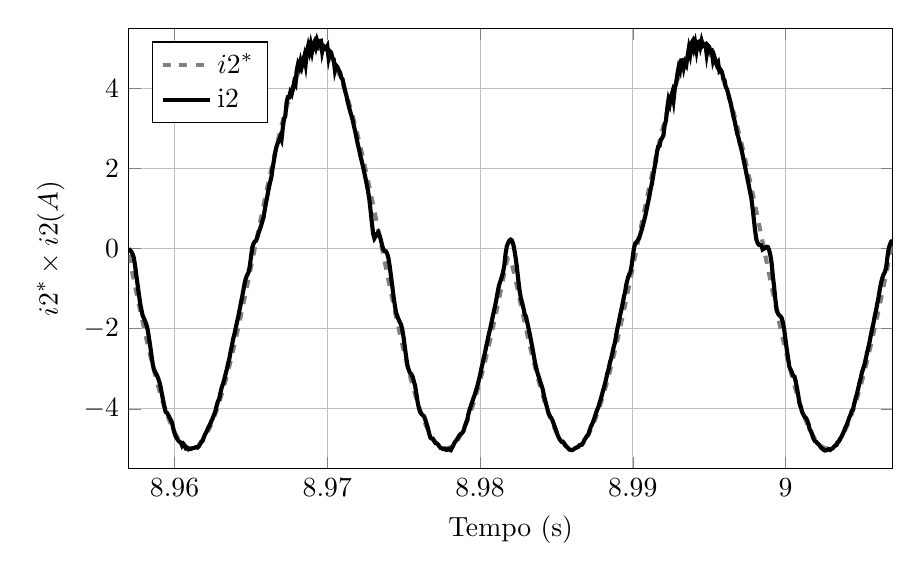
\begin{tikzpicture}

\begin{axis}[%
width=0.8\textwidth,
height=0.461611624834875\textwidth,
scale only axis,
xmin=8.957,
xmax=9.007,
xtick={8.96, 8.97, 8.98, 8.99,    9},
xlabel={Tempo (s)},
xmajorgrids,
ymin=-5.5,
ymax=5.5,
ytick={-4, -2,  0,  2,  4},
ylabel={$\text{i2}^\text{*}\text{ }\times\text{ i2 (A)}$},
ymajorgrids,
legend style={at={(0.03,0.97)},anchor=north west,draw=black,fill=white,legend cell align=left}
]
\addplot [color=gray,dashed,line width=1.5pt]
  table[row sep=crcr]{8.9570000023925	-0.157053337715654\\
8.95708334239271	-0.313642611979098\\
8.95716665239292	-0.469922358851051\\
8.95724999239313	-0.625738349089232\\
8.95733333239333	-0.780936811123168\\
8.95741667239354	-0.935364582808169\\
8.95749998239375	-1.08886926257787\\
8.95758332239396	-1.24129935984619\\
8.95766666239417	-1.39250444451023\\
8.95775000239438	-1.54233529540664\\
8.95783334239458	-1.69064404757487\\
8.95791665239479	-1.83728433818208\\
8.957999992395	-1.98211145096553\\
8.95808333239521	-2.1249824590501\\
8.95816667239542	-2.26575636599982\\
8.95824998239562	-2.40429424496438\\
8.95833332239583	-2.54045937578312\\
8.95841666239604	-2.67411737991134\\
8.95850000239625	-2.8051363530357\\
8.95858334239646	-2.93338699524782\\
8.95866665239667	-3.05874273864774\\
8.95874999239688	-3.1810798722511\\
8.95883333239708	-3.30027766407697\\
8.95891667239729	-3.41621848029576\\
8.9589999823975	-3.52878790131954\\
8.95908332239771	-3.63787483472045\\
8.95916666239792	-3.74337162486544\\
8.95925000239813	-3.84517415915942\\
8.95933334239833	-3.94318197079182\\
8.95941665239854	-4.03729833788517\\
8.95949999239875	-4.12743037894796\\
8.95958333239896	-4.21348914453744\\
8.95966667239917	-4.29538970504198\\
8.95974998239937	-4.37305123449631\\
8.95983332239958	-4.44639709034708\\
8.95991666239979	-4.5153548890897\\
8.9600000024	-4.57985657770219\\
8.96008334240021	-4.63983850080527\\
8.96016665240042	-4.69524146348255\\
8.96024999240062	-4.74601078969874\\
8.96033333240083	-4.79209637625833\\
8.96041667240104	-4.83345274225136\\
8.96049998240125	-4.8700390739376\\
8.96058332240146	-4.90181926502482\\
8.96066666240167	-4.92876195230126\\
8.96075000240188	-4.95084054658743\\
8.96083334240208	-4.96803325897633\\
8.96091665240229	-4.98032312233656\\
8.9609999924025	-4.98769800805673\\
8.96108333240271	-4.99015063801503\\
8.96116667240292	-4.98767859176179\\
8.96124998240312	-4.98028430890822\\
8.96133332240333	-4.96797508671877\\
8.96141666240354	-4.95076307290963\\
8.96150000240375	-4.9286652536604\\
8.96158334240396	-4.90170343685077\\
8.96166665240417	-4.8699042305388\\
8.96174999240437	-4.83329901670194\\
8.96183333240458	-4.79192392026687\\
8.96191667240479	-4.74581977345848\\
8.961999982405	-4.69503207550345\\
8.96208332240521	-4.63961094772799\\
8.96216666240542	-4.57961108409414\\
8.96225000240563	-4.51509169722343\\
8.96233334240583	-4.44611645996119\\
8.96241665240604	-4.37275344253912\\
8.96249999240625	-4.29507504539818\\
8.96258333240646	-4.21315792773813\\
8.96266667240667	-4.12708293186412\\
8.96274998240687	-4.03693500340512\\
8.96283332240708	-3.94280310748283\\
8.96291666240729	-3.84478014091384\\
8.9630000024075	-3.74296284053171\\
8.96308334240771	-3.63745168771934\\
8.96316665240792	-3.52835080924607\\
8.96324999240812	-3.41576787450702\\
8.96333333240833	-3.29981398926649\\
8.96341667240854	-3.18060358600992\\
8.96349998240875	-3.05825431101288\\
8.96358332240896	-2.9328869082384\\
8.96366666240917	-2.80462510017721\\
8.96375000240938	-2.67359546574863\\
8.96383334240958	-2.53992731538246\\
8.96391665240979	-2.40375256340514\\
8.96399999241	-2.26520559785631\\
8.96408333241021	-2.12442314786397\\
8.96416667241042	-1.98154414870942\\
8.96424998241062	-1.8367096047148\\
8.96433332241083	-1.69006245008898\\
8.96441666241104	-1.54174740786863\\
8.96450000241125	-1.39191084709413\\
8.96458334241146	-1.24070063836098\\
8.96466665241167	-1.08826600788938\\
8.96474999241187	-0.934757390255931\\
8.96483333241208	-0.78032627993293\\
8.96491667241229	-0.62512508178157\\
8.9649999824125	-0.469306960646756\\
8.96508332241271	-0.313025690201901\\
8.96516666241292	-0.156435501192865\\
8.96525000241313	0.000309070769160563\\
8.96533334241333	0.157053337715652\\
8.96541665241354	0.313642611979097\\
8.96549999241375	0.46992235885105\\
8.96558333241396	0.625738349089232\\
8.96566667241417	0.780936811123168\\
8.96574998241437	0.93536458280817\\
8.96583332241458	1.08886926257787\\
8.96591666241479	1.24129935984619\\
8.966000002415	1.39250444451023\\
8.96608334241521	1.54233529540664\\
8.96616665241542	1.69064404757488\\
8.96624999241562	1.83728433818209\\
8.96633333241583	1.98211145096554\\
8.96641667241604	2.1249824590501\\
8.96649998241625	2.26575636599983\\
8.96658332241646	2.40429424496439\\
8.96666666241667	2.54045937578313\\
8.96675000241687	2.67411737991135\\
8.96683334241708	2.80513635303571\\
8.96691665241729	2.93338699524783\\
8.9669999924175	3.05874273864775\\
8.96708333241771	3.18107987225111\\
8.96716667241792	3.30027766407699\\
8.96724998241812	3.41621848029577\\
8.96733332241833	3.52878790131955\\
8.96741666241854	3.63787483472046\\
8.96750000241875	3.74337162486546\\
8.96758334241896	3.84517415915944\\
8.96766665241917	3.94318197079183\\
8.96774999241937	4.03729833788518\\
8.96783333241958	4.12743037894798\\
8.96791667241979	4.21348914453746\\
8.96799998242	4.29538970504199\\
8.96808332242021	4.37305123449633\\
8.96816666242042	4.4463970903471\\
8.96825000242062	4.51535488908972\\
8.96833334242083	4.57985657770221\\
8.96841665242104	4.63983850080529\\
8.96849999242125	4.69524146348257\\
8.96858333242146	4.74601078969876\\
8.96866667242167	4.79209637625835\\
8.96874998242187	4.83345274225138\\
8.96883332242208	4.87003907393763\\
8.96891666242229	4.90181926502484\\
8.9690000024225	4.92876195230128\\
8.96908334242271	4.95084054658745\\
8.96916665242292	4.96803325897636\\
8.96924999242312	4.98032312233658\\
8.96933333242333	4.98769800805675\\
8.96941667242354	4.99015063801505\\
8.96949998242375	4.98767859176182\\
8.96958332242396	4.98028430890825\\
8.96966666242417	4.9679750867188\\
8.96975000242437	4.95076307290965\\
8.96983334242458	4.92866525366042\\
8.96991665242479	4.90170343685079\\
8.969999992425	4.86990423053882\\
8.97008333242521	4.83329901670197\\
8.97016667242542	4.79192392026689\\
8.97024998242562	4.7458197734585\\
8.97033332242583	4.69503207550347\\
8.97041666242604	4.63961094772801\\
8.97050000242625	4.57961108409416\\
8.97058334242646	4.51509169722345\\
8.97066665242667	4.44611645996121\\
8.97074999242687	4.37275344253914\\
8.97083333242708	4.2950750453982\\
8.97091667242729	4.21315792773815\\
8.9709999824275	4.12708293186414\\
8.97108332242771	4.03693500340514\\
8.97116666242792	3.94280310748285\\
8.97125000242812	3.84478014091386\\
8.97133334242833	3.74296284053172\\
8.97141665242854	3.63745168771936\\
8.97149999242875	3.52835080924608\\
8.97158333242896	3.41576787450704\\
8.97166667242917	3.2998139892665\\
8.97174998242937	3.18060358600993\\
8.97183332242958	3.0582543110129\\
8.97191666242979	2.93288690823841\\
8.97200000243	2.80462510017722\\
8.97208334243021	2.67359546574865\\
8.97216665243042	2.53992731538247\\
8.97224999243062	2.40375256340515\\
8.97233333243083	2.26520559785632\\
8.97241667243104	2.12442314786398\\
8.97249998243125	1.98154414870943\\
8.97258332243146	1.83670960471481\\
8.97266666243167	1.69006245008899\\
8.97275000243187	1.54174740786863\\
8.97283334243208	1.39191084709414\\
8.97291665243229	1.24070063836099\\
8.9729999924325	1.08826600788938\\
8.97308333243271	0.934757390255936\\
8.97316667243292	0.780326279932935\\
8.97324998243312	0.625125081781573\\
8.97333332243333	0.469306960646759\\
8.97341666243354	0.313025690201903\\
8.97350000243375	0.156435501192867\\
8.97358334243396	-0.000309070769160008\\
8.97366665243417	-0.157053337715652\\
8.97374999243437	-0.313642611979098\\
8.97383333243458	-0.469922358851052\\
8.97391667243479	-0.625738349089234\\
8.973999982435	-0.780936811123171\\
8.97408332243521	-0.935364582808174\\
8.97416666243542	-1.08886926257788\\
8.97425000243562	-1.2412993598462\\
8.97433334243583	-1.39250444451024\\
8.97441665243604	-1.54233529540665\\
8.97449999243625	-1.69064404757489\\
8.97458333243646	-1.8372843381821\\
8.97466667243667	-1.98211145096555\\
8.97474998243687	-2.12498245905011\\
8.97483332243708	-2.26575636599984\\
8.97491666243729	-2.4042942449644\\
8.9750000024375	-2.54045937578314\\
8.97508334243771	-2.67411737991137\\
8.97516665243792	-2.80513635303572\\
8.97524999243812	-2.93338699524785\\
8.97533333243833	-3.05874273864777\\
8.97541667243854	-3.18107987225113\\
8.97549998243875	-3.300277664077\\
8.97558332243896	-3.41621848029578\\
8.97566666243917	-3.52878790131957\\
8.97575000243937	-3.63787483472048\\
8.97583334243958	-3.74337162486547\\
8.97591665243979	-3.84517415915946\\
8.97599999244	-3.94318197079185\\
8.97608333244021	-4.0372983378852\\
8.97616667244042	-4.127430378948\\
8.97624998244062	-4.21348914453748\\
8.97633332244083	-4.29538970504201\\
8.97641666244104	-4.37305123449635\\
8.97650000244125	-4.44639709034712\\
8.97658334244146	-4.51535488908974\\
8.97666665244167	-4.57985657770223\\
8.97674999244187	-4.63983850080531\\
8.97683333244208	-4.69524146348259\\
8.97691667244229	-4.74601078969879\\
8.9769999824425	-4.79209637625837\\
8.97708332244271	-4.8334527422514\\
8.97716666244292	-4.87003907393765\\
8.97725000244312	-4.90181926502486\\
8.97733334244333	-4.92876195230131\\
8.97741665244354	-4.95084054658747\\
8.97749999244375	-4.96803325897638\\
8.97758333244396	-4.9803231223366\\
8.97766667244417	-4.98769800805677\\
8.97774998244438	-4.99015063801507\\
8.97783332244458	-4.98767859176184\\
8.97791666244479	-4.98028430890827\\
8.978000002445	-4.96797508671882\\
8.97808334244521	-4.95076307290968\\
8.97816665244542	-4.92866525366044\\
8.97824999244562	-4.90170343685081\\
8.97833333244583	-4.86990423053884\\
8.97841667244604	-4.83329901670199\\
8.97849998244625	-4.79192392026691\\
8.97858332244646	-4.74581977345852\\
8.97866666244667	-4.69503207550349\\
8.97875000244687	-4.63961094772803\\
8.97883334244708	-4.57961108409418\\
8.97891665244729	-4.51509169722347\\
8.9789999924475	-4.44611645996123\\
8.97908333244771	-4.37275344253916\\
8.97916667244792	-4.29507504539822\\
8.97924998244813	-4.21315792773817\\
8.97933332244833	-4.12708293186416\\
8.97941666244854	-4.03693500340516\\
8.97950000244875	-3.94280310748287\\
8.97958334244896	-3.84478014091388\\
8.97966665244917	-3.74296284053174\\
8.97974999244937	-3.63745168771938\\
8.97983333244958	-3.5283508092461\\
8.97991667244979	-3.41576787450705\\
8.97999998245	-3.29981398926652\\
8.98008332245021	-3.18060358600995\\
8.98016666245042	-3.05825431101291\\
8.98025000245062	-2.93288690823843\\
8.98033334245083	-2.80462510017723\\
8.98041665245104	-2.67359546574866\\
8.98049999245125	-2.53992731538248\\
8.98058333245146	-2.40375256340516\\
8.98066667245167	-2.26520559785633\\
8.98074998245188	-2.124423147864\\
8.98083332245208	-1.98154414870944\\
8.98091666245229	-1.83670960471482\\
8.9810000024525	-1.690062450089\\
8.98108334245271	-1.54174740786864\\
8.98116665245292	-1.39191084709414\\
8.98124999245312	-1.24070063836099\\
8.98133333245333	-1.08826600788939\\
8.98141667245354	-0.934757390255941\\
8.98149998245375	-0.780326279932939\\
8.98158332245396	-0.625125081781577\\
8.98166666245417	-0.469306960646762\\
8.98175000245437	-0.313025690201905\\
8.98183334245458	-0.234962398887561\\
8.98191665245479	-0.235194125748636\\
8.981999992455	-0.294088917675021\\
8.98208333245521	-0.391956928193599\\
8.98216667245542	-0.513977780075711\\
8.98224998245563	-0.650215191260269\\
8.98233332245583	-0.794399797988042\\
8.98241666245604	-0.942708359130287\\
8.98250000245625	-1.09284729218378\\
8.98258334245646	-1.24344144537157\\
8.98266665245667	-1.39365202263414\\
8.98274999245687	-1.5429473521492\\
8.98283333245708	-1.69096920978647\\
8.98291667245729	-1.83745648620804\\
8.9829999824575	-1.9822023084386\\
8.98308332245771	-2.12503027951668\\
8.98316666245792	-2.26578147209814\\
8.98325000245812	-2.40430739594607\\
8.98333334245833	-2.54046625024024\\
8.98341665245854	-2.67412096662305\\
8.98349999245875	-2.80513822113313\\
8.98358333245896	-2.93338796666734\\
8.98366667245917	-3.05874324304291\\
8.98374998245938	-3.1810801337914\\
8.98383332245958	-3.30027779951849\\
8.98391666245979	-3.41621855035221\\
8.98400000246	-3.52878793751563\\
8.98408334246021	-3.63787485340244\\
8.98416665246042	-3.74337163449842\\
8.98424999246063	-3.84517416412192\\
8.98433333246083	-3.94318197334608\\
8.98441667246104	-4.03729833919882\\
8.98449998246125	-4.12743037962306\\
8.98458332246146	-4.21348914488415\\
8.98466666246167	-4.29538970521992\\
8.98475000246187	-4.3730512345876\\
8.98483334246208	-4.44639709039389\\
8.98491665246229	-4.51535488911371\\
8.9849999924625	-4.57985657771451\\
8.98508333246271	-4.63983850081161\\
8.98516667246292	-4.69524146348582\\
8.98524998246313	-4.74601078970045\\
8.98533332246333	-4.79209637625923\\
8.98541666246354	-4.83345274225185\\
8.98550000246375	-4.87003907393789\\
8.98558334246396	-4.90181926502499\\
8.98566665246417	-4.92876195230139\\
8.98574999246438	-4.95084054658752\\
8.98583333246458	-4.96803325897642\\
8.98591667246479	-4.98032312233663\\
8.985999982465	-4.9876980080568\\
8.98608332246521	-4.9901506380151\\
8.98616666246542	-4.98767859176186\\
8.98625000246562	-4.98028430890829\\
8.98633334246583	-4.96797508671884\\
8.98641665246604	-4.9507630729097\\
8.98649999246625	-4.92866525366047\\
8.98658333246646	-4.90170343685084\\
8.98666667246667	-4.86990423053886\\
8.98674998246688	-4.83329901670201\\
8.98683332246708	-4.79192392026693\\
8.98691666246729	-4.74581977345854\\
8.9870000024675	-4.69503207550351\\
8.98708334246771	-4.63961094772805\\
8.98716665246792	-4.5796110840942\\
8.98724999246813	-4.51509169722349\\
8.98733333246833	-4.44611645996125\\
8.98741667246854	-4.37275344253918\\
8.98749998246875	-4.29507504539824\\
8.98758332246896	-4.21315792773819\\
8.98766666246917	-4.12708293186418\\
8.98775000246937	-4.03693500340518\\
8.98783334246958	-3.94280310748288\\
8.98791665246979	-3.8447801409139\\
8.98799999247	-3.74296284053176\\
8.98808333247021	-3.63745168771939\\
8.98816667247042	-3.52835080924612\\
8.98824998247063	-3.41576787450707\\
8.98833332247083	-3.29981398926653\\
8.98841666247104	-3.18060358600996\\
8.98850000247125	-3.05825431101293\\
8.98858334247146	-2.93288690823844\\
8.98866665247167	-2.80462510017725\\
8.98874999247188	-2.67359546574867\\
8.98883333247208	-2.53992731538249\\
8.98891667247229	-2.40375256340517\\
8.9889999824725	-2.26520559785634\\
8.98908332247271	-2.124423147864\\
8.98916666247292	-1.98154414870944\\
8.98925000247313	-1.83670960471483\\
8.98933334247333	-1.690062450089\\
8.98941665247354	-1.54174740786865\\
8.98949999247375	-1.39191084709415\\
8.98958333247396	-1.240700638361\\
8.98966667247417	-1.08826600788939\\
8.98974998247438	-0.934757390255946\\
8.98983332247458	-0.780326279932943\\
8.98991666247479	-0.625125081781581\\
8.990000002475	-0.469306960646765\\
8.99008334247521	-0.313025690201907\\
8.99016665247542	-0.15643550119287\\
8.99024999247563	0.000309070769158107\\
8.99033333247583	0.157053337715651\\
8.99041667247604	0.313642611979099\\
8.99049998247625	0.469922358851054\\
8.99058332247646	0.625738349089237\\
8.99066666247667	0.780936811123176\\
8.99075000247688	0.93536458280818\\
8.99083334247708	1.08886926257789\\
8.99091665247729	1.24129935984621\\
8.9909999924775	1.39250444451025\\
8.99108333247771	1.54233529540666\\
8.99116667247792	1.6906440475749\\
8.99124998247813	1.83728433818211\\
8.99133332247833	1.98211145096556\\
8.99141666247854	2.12498245905013\\
8.99150000247875	2.26575636599985\\
8.99158334247896	2.40429424496442\\
8.99166665247917	2.54045937578316\\
8.99174999247938	2.67411737991139\\
8.99183333247958	2.80513635303574\\
8.99191667247979	2.93338699524787\\
8.99199998248	3.05874273864779\\
8.99208332248021	3.18107987225115\\
8.99216666248042	3.30027766407703\\
8.99225000248063	3.41621848029581\\
8.99233334248083	3.5287879013196\\
8.99241665248104	3.63787483472051\\
8.99249999248125	3.7433716248655\\
8.99258333248146	3.84517415915949\\
8.99266667248167	3.94318197079189\\
8.99274998248188	4.03729833788524\\
8.99283332248208	4.12743037894803\\
8.99291666248229	4.21348914453752\\
8.9930000024825	4.29538970504205\\
8.99308334248271	4.37305123449639\\
8.99316665248292	4.44639709034716\\
8.99324999248313	4.51535488908978\\
8.99333333248333	4.57985657770227\\
8.99341667248354	4.63983850080535\\
8.99349998248375	4.69524146348263\\
8.99358332248396	4.74601078969883\\
8.99366666248417	4.79209637625842\\
8.99375000248438	4.83345274225144\\
8.99383334248458	4.87003907393769\\
8.99391665248479	4.9018192650249\\
8.993999992485	4.92876195230135\\
8.99408333248521	4.95084054658752\\
8.99416667248542	4.96803325897642\\
8.99424998248563	4.98032312233665\\
8.99433332248583	4.98769800805682\\
8.99441666248604	4.99015063801512\\
8.99450000248625	4.98767859176188\\
8.99458334248646	4.98028430890831\\
8.99466665248667	4.96797508671886\\
8.99474999248688	4.95076307290972\\
8.99483333248708	4.92866525366049\\
8.99491667248729	4.90170343685086\\
8.9949999824875	4.86990423053888\\
8.99508332248771	4.83329901670203\\
8.99516666248792	4.79192392026696\\
8.99525000248813	4.74581977345856\\
8.99533334248833	4.69503207550353\\
8.99541665248854	4.63961094772807\\
8.99549999248875	4.57961108409422\\
8.99558333248896	4.51509169722351\\
8.99566667248917	4.44611645996127\\
8.99574998248938	4.3727534425392\\
8.99583332248958	4.29507504539826\\
8.99591666248979	4.2131579277382\\
8.99600000249	4.12708293186419\\
8.99608334249021	4.03693500340519\\
8.99616665249042	3.9428031074829\\
8.99624999249063	3.84478014091391\\
8.99633333249083	3.74296284053177\\
8.99641667249104	3.63745168771941\\
8.99649998249125	3.52835080924613\\
8.99658332249146	3.41576787450708\\
8.99666666249167	3.29981398926655\\
8.99675000249188	3.18060358600998\\
8.99683334249208	3.05825431101294\\
8.99691665249229	2.93288690823845\\
8.9969999924925	2.80462510017726\\
8.99708333249271	2.67359546574868\\
8.99716667249292	2.53992731538251\\
8.99724998249313	2.40375256340519\\
8.99733332249333	2.26520559785635\\
8.99741666249354	2.12442314786402\\
8.99750000249375	1.98154414870945\\
8.99758334249396	1.83670960471484\\
8.99766665249417	1.69006245008901\\
8.99774999249438	1.54174740786866\\
8.99783333249458	1.39191084709416\\
8.99791667249479	1.24070063836101\\
8.997999982495	1.0882660078894\\
8.99808332249521	0.934757390255951\\
8.99816666249542	0.780326279932948\\
8.99825000249563	0.625125081781584\\
8.99833334249583	0.469306960646768\\
8.99841665249604	0.31302569020191\\
8.99849999249625	0.156435501192872\\
8.99858333249646	-0.000309070769156955\\
8.99866667249667	-0.157053337715651\\
8.99874998249688	-0.313642611979099\\
8.99883332249708	-0.469922358851055\\
8.99891666249729	-0.625738349089239\\
8.9990000024975	-0.780936811123178\\
8.99908334249771	-0.935364582808183\\
8.99916665249792	-1.08886926257789\\
8.99924999249813	-1.24129935984621\\
8.99933333249833	-1.39250444451026\\
8.99941667249854	-1.54233529540666\\
8.99949998249875	-1.6906440475749\\
8.99958332249896	-1.83728433818212\\
8.99966666249917	-1.98211145096557\\
8.99975000249938	-2.12498245905014\\
8.99983334249958	-2.26575636599986\\
8.99991665249979	-2.40429424496443\\
8.9999999925	-2.54045937578317\\
9.00008333250021	-2.6741173799114\\
9.00016667250042	-2.80513635303576\\
9.00024998250063	-2.93338699524788\\
9.00033332250083	-3.0587427386478\\
9.00041666250104	-3.18107987225116\\
9.00050000250125	-3.30027766407704\\
9.00058334250146	-3.41621848029583\\
9.00066665250167	-3.52878790131961\\
9.00074999250188	-3.63787483472053\\
9.00083333250208	-3.74337162486552\\
9.00091667250229	-3.8451741591595\\
9.0009999825025	-3.9431819707919\\
9.00108332250271	-4.03729833788526\\
9.00116666250292	-4.12743037894805\\
9.00125000250313	-4.21348914453753\\
9.00133334250333	-4.29538970504207\\
9.00141665250354	-4.37305123449641\\
9.00149999250375	-4.44639709034718\\
9.00158333250396	-4.5153548890898\\
9.00166667250417	-4.57985657770229\\
9.00174998250438	-4.63983850080537\\
9.00183332250458	-4.69524146348265\\
9.00191666250479	-4.74601078969885\\
9.002000002505	-4.79209637625844\\
9.00208334250521	-4.83345274225146\\
9.00216665250542	-4.87003907393771\\
9.00224999250563	-4.90181926502493\\
9.00233333250583	-4.92876195230137\\
9.00241667250604	-4.95084054658754\\
9.00249998250625	-4.96803325897644\\
9.00258332250646	-4.98032312233667\\
9.00266666250667	-4.98769800805684\\
9.00275000250688	-4.99015063801514\\
9.00283334250708	-4.9876785917619\\
9.00291665250729	-4.98028430890833\\
9.0029999925075	-4.96797508671888\\
9.00308333250771	-4.95076307290974\\
9.00316667250792	-4.92866525366051\\
9.00324998250812	-4.90170343685088\\
9.00333332250833	-4.8699042305389\\
9.00341666250854	-4.83329901670205\\
9.00350000250875	-4.79192392026698\\
9.00358334250896	-4.74581977345858\\
9.00366665250917	-4.69503207550355\\
9.00374999250938	-4.63961094772809\\
9.00383333250958	-4.57961108409424\\
9.00391667250979	-4.51509169722353\\
9.00399998251	-4.44611645996129\\
9.00408332251021	-4.37275344253922\\
9.00416666251042	-4.29507504539828\\
9.00425000251063	-4.21315792773822\\
9.00433334251083	-4.12708293186421\\
9.00441665251104	-4.03693500340521\\
9.00449999251125	-3.94280310748292\\
9.00458333251146	-3.84478014091393\\
9.00466667251167	-3.74296284053179\\
9.00474998251187	-3.63745168771943\\
9.00483332251208	-3.52835080924615\\
9.00491666251229	-3.4157678745071\\
9.0050000025125	-3.29981398926656\\
9.00508334251271	-3.18060358600999\\
9.00516665251292	-3.05825431101296\\
9.00524999251313	-2.93288690823847\\
9.00533333251333	-2.80462510017727\\
9.00541667251354	-2.6735954657487\\
9.00549998251375	-2.53992731538252\\
9.00558332251396	-2.4037525634052\\
9.00566666251417	-2.26520559785636\\
9.00575000251438	-2.12442314786403\\
9.00583334251458	-1.98154414870946\\
9.00591665251479	-1.83670960471485\\
9.005999992515	-1.69006245008902\\
9.00608333251521	-1.54174740786867\\
9.00616667251542	-1.39191084709417\\
9.00624998251562	-1.24070063836102\\
9.00633332251583	-1.08826600788941\\
9.00641666251604	-0.934757390255958\\
9.00650000251625	-0.780326279932954\\
9.00658334251646	-0.62512508178159\\
9.00666665251667	-0.469306960646773\\
9.00674999251688	-0.313025690201914\\
9.00683333251708	-0.156435501192875\\
9.00691667251729	0.000309070769154721\\
9.0069999825175	0.15705333771565\\
};
\addlegendentry{$\text{i2}^\text{*}$};

\addplot [color=black,solid,line width=1.5pt]
  table[row sep=crcr]{8.9570000023925	-0.00330524129232349\\
8.95708334239271	-0.0428438155110735\\
8.95716665239292	-0.0741243330891985\\
8.95724999239313	-0.137436100667323\\
8.95733333239333	-0.227523991292323\\
8.95741667239354	-0.420962711995448\\
8.95749998239375	-0.676211735432948\\
8.95758332239396	-0.907937809651698\\
8.95766666239417	-1.14091510457357\\
8.95775000239438	-1.3683870284017\\
8.95783334239458	-1.53304767293295\\
8.95791665239479	-1.6756868330892\\
8.957999992395	-1.74425372762045\\
8.95808333239521	-1.8218294112142\\
8.95816667239542	-1.90541095418295\\
8.95824998239562	-2.04254474324545\\
8.95833332239583	-2.2462434737142\\
8.95841666239604	-2.45519733113607\\
8.95850000239625	-2.6936799971517\\
8.95858334239646	-2.91264362019857\\
8.95866665239667	-3.02775592488607\\
8.95874999239688	-3.09432086629232\\
8.95883333239708	-3.1511262862142\\
8.95891667239729	-3.22594928426107\\
8.9589999823975	-3.32054156941732\\
8.95908332239771	-3.44516315144857\\
8.95916666239792	-3.61808185262045\\
8.95925000239813	-3.7787385909017\\
8.95933334239833	-3.9408967940267\\
8.95941665239854	-4.07677936238607\\
8.95949999239875	-4.09955157918295\\
8.95958333239896	-4.14734821004232\\
8.95966667239917	-4.21541461629232\\
8.95974998239937	-4.27272052449545\\
8.95983332239958	-4.34404010457357\\
8.95991666239979	-4.48717975301107\\
8.9600000024	-4.61080035847982\\
8.96008334240021	-4.69388141316732\\
8.96016665240042	-4.74643268269857\\
8.96024999240062	-4.79422931355795\\
8.96033333240083	-4.82225665730795\\
8.96041667240104	-4.84302692097982\\
8.96049998240125	-4.9218538252767\\
8.96058332240146	-4.87555865926107\\
8.96066666240167	-4.91734943074545\\
8.96075000240188	-4.98841876668295\\
8.96083334240208	-4.97315387410482\\
8.96091665240229	-5.0099397627767\\
8.9609999924025	-4.99542560262045\\
8.96108333240271	-4.99942950887045\\
8.96116667240292	-4.98316363972982\\
8.96124998240312	-4.9779085127767\\
8.96133332240333	-4.96739825887045\\
8.96141666240354	-4.9538850752767\\
8.96150000240375	-4.9678987471517\\
8.96158334240396	-4.94162311238607\\
8.96166665240417	-4.88106403035482\\
8.96174999240437	-4.81925372762045\\
8.96183333240458	-4.79823321980795\\
8.96191667240479	-4.7126497237142\\
8.961999982405	-4.6335725752767\\
8.96208332240521	-4.5805208174642\\
8.96216666240542	-4.49919147176107\\
8.96225000240563	-4.4403840987142\\
8.96233334240583	-4.37557086629232\\
8.96241665240604	-4.3012483565267\\
8.96249999240625	-4.2321809737142\\
8.96258333240646	-4.14659747762045\\
8.96266667240667	-4.06551837605795\\
8.96274998240687	-3.93739337605795\\
8.96283332240708	-3.81827716512045\\
8.96291666240729	-3.7597200362142\\
8.9630000024075	-3.6105745284017\\
8.96308334240771	-3.47118854207357\\
8.96316665240792	-3.38385333699545\\
8.96324999240812	-3.2742464034017\\
8.96333333240833	-3.14361896199545\\
8.96341667240854	-3.02325153035482\\
8.96349998240875	-2.87710895222982\\
8.96358332240896	-2.75348834676107\\
8.96366666240917	-2.57906818074545\\
8.96375000240938	-2.43167438191732\\
8.96383334240958	-2.26150836629232\\
8.96391665240979	-2.13738727254232\\
8.96399999241	-1.99224567097982\\
8.96408333241021	-1.84410113972982\\
8.96416667241042	-1.7067171065267\\
8.96424998241062	-1.54480914754232\\
8.96433332241083	-1.3773958174642\\
8.96441666241104	-1.2212434737142\\
8.96450000241125	-1.0520784346517\\
8.96458334241146	-0.873153874104823\\
8.96466665241167	-0.741525456136073\\
8.96474999241187	-0.661697575276698\\
8.96483333241208	-0.607144352620448\\
8.96491667241229	-0.459750553792323\\
8.9649999824125	-0.227523991292323\\
8.96508332241271	0.0204679520670515\\
8.96516666241292	0.118063166910802\\
8.96525000241313	0.174368098551426\\
8.96533334241333	0.192886164957676\\
8.96541665241354	0.278469661051427\\
8.96549999241375	0.390078547770176\\
8.96558333241396	0.477663996988926\\
8.96566667241417	0.573007014567052\\
8.96574998241437	0.682613948160801\\
8.96583332241458	0.787716487223301\\
8.96591666241479	0.990664485270176\\
8.966000002415	1.1650846512858\\
8.96608334241521	1.33249798136393\\
8.96616665241542	1.50066204386393\\
8.96624999241562	1.6485563309733\\
8.96633333241583	1.77042522745768\\
8.96641667241604	1.99914837198893\\
8.96649998241625	2.18858318644205\\
8.96658332241646	2.37901897745768\\
8.96666666241667	2.5324186356608\\
8.96675000241687	2.63076458292643\\
8.96683334241708	2.6955778153483\\
8.96691665241729	2.79042034464518\\
8.9669999924175	2.71709881144205\\
8.96708333241771	3.0008756669108\\
8.96716667241792	3.23660564737955\\
8.96724998241812	3.3051725419108\\
8.96733332241833	3.64475384073893\\
8.96741666241854	3.77713299112955\\
8.96750000241875	3.77788372355143\\
8.96758334241896	3.9077604325358\\
8.96766665241917	3.85195598917643\\
8.96774999241937	3.98158245402018\\
8.96783333241958	4.1560026200358\\
8.96791667241979	4.10169964152018\\
8.96799998242	4.4542936356608\\
8.96808332242021	4.60318889933268\\
8.96816666242042	4.52586345987955\\
8.96825000242062	4.67776165323893\\
8.96833334242083	4.54688396769205\\
8.96841665242104	4.6725065262858\\
8.96849999242125	4.80213299112955\\
8.96858333242146	4.61094646769205\\
8.96866667242167	4.91199016886393\\
8.96874998242187	5.0578825028483\\
8.96883332242208	4.91999798136393\\
8.96891666242229	5.08966350870768\\
8.9690000024225	4.9187467606608\\
8.96908334242271	5.09917278605143\\
8.96916665242292	5.16473675089518\\
8.96924999242312	5.03811321573893\\
8.96933333242333	5.19251385050455\\
8.96941667242354	5.09316692667643\\
8.96949998242375	5.1759977372233\\
8.96958332242396	5.18475628214518\\
8.96966666242417	4.91499309855143\\
8.96975000242437	5.05613079386393\\
8.96983334242458	5.02359905558268\\
8.96991665242479	4.9868131669108\\
8.969999992425	5.04562053995768\\
8.97008333242521	4.7686002762858\\
8.97016667242542	4.9277555497233\\
8.97024998242562	4.89647503214518\\
8.97033332242583	4.7595914872233\\
8.97041666242604	4.7275602372233\\
8.97050000242625	4.44678631144205\\
8.97058334242646	4.56815471964518\\
8.97066665242667	4.52811565714518\\
8.97074999242687	4.4572965653483\\
8.97083333242708	4.39498577433268\\
8.97091667242729	4.26535930948893\\
8.9709999824275	4.2250700028483\\
8.97108332242771	4.07267132120768\\
8.97116666242792	3.93328533487955\\
8.97125000242812	3.81917400675455\\
8.97133334242833	3.66302166300455\\
8.97141665242854	3.53714886027018\\
8.97149999242875	3.42103557902018\\
8.97158333242896	3.31393108683268\\
8.97166667242917	3.1930631669108\\
8.97174998242937	3.05042400675455\\
8.97183332242958	2.91303997355143\\
8.97191666242979	2.75638714152018\\
8.97200000243	2.59923382120768\\
8.97208334243021	2.47010784464518\\
8.97216665243042	2.30970135050455\\
8.97224999243062	2.18858318644205\\
8.97233333243083	2.0529508622233\\
8.97241667243104	1.90906048136393\\
8.97249998243125	1.75641155558268\\
8.97258332243146	1.59725628214518\\
8.97266666243167	1.43659954386393\\
8.97275000243187	1.23139934855143\\
8.97283334243208	0.949123957926426\\
8.97291665243229	0.648580745035801\\
8.9729999924325	0.372060969645176\\
8.97308333243271	0.256448176676427\\
8.97316667243292	0.309249690348301\\
8.97324998243312	0.366555598551427\\
8.97333332243333	0.406594661051427\\
8.97341666243354	0.329769709879552\\
8.97350000243375	0.221413996988927\\
8.97358334243396	0.0877836258951765\\
8.97366665243417	-0.0163179366048235\\
8.97374999243437	-0.0616121260579485\\
8.97383333243458	-0.0676179854329485\\
8.97391667243479	-0.122421452229823\\
8.973999982435	-0.235281559651698\\
8.97408332243521	-0.437228581136073\\
8.97416666243542	-0.681216618245448\\
8.97425000243562	-0.927206608479823\\
8.97433334243583	-1.1832063643392\\
8.97441665243604	-1.40467242879232\\
8.97449999243625	-1.59385699910482\\
8.97458333243646	-1.68244342488607\\
8.97466667243667	-1.7697786299642\\
8.97474998243687	-1.8418489424642\\
8.97483332243708	-1.89915485066732\\
8.97491666243729	-2.04179401082357\\
8.9750000024375	-2.23648395222982\\
8.97508334243771	-2.4814729659017\\
8.97516665243792	-2.71545123738607\\
8.97524999243812	-2.9239046065267\\
8.97533333243833	-3.02925738972982\\
8.97541667243854	-3.10633258504232\\
8.97549998243875	-3.13160724324545\\
8.97558332243896	-3.19541949910482\\
8.97566666243917	-3.3152864424642\\
8.97575000243937	-3.42789630574545\\
8.97583334243958	-3.6275911299642\\
8.97591665243979	-3.84004840535482\\
8.97599999244	-3.98744220418295\\
8.97608333244021	-4.08453693074545\\
8.97616667244042	-4.1310823409017\\
8.97624998244062	-4.1591096846517\\
8.97633332244083	-4.1861360518392\\
8.97641666244104	-4.2722200362142\\
8.97650000244125	-4.37081622762045\\
8.97658334244146	-4.4814241377767\\
8.97666665244167	-4.61180133504232\\
8.97674999244187	-4.72090778035482\\
8.97683333244208	-4.7416780440267\\
8.97691667244229	-4.7536897627767\\
8.9769999824425	-4.80824298543295\\
8.97708332244271	-4.85628986043295\\
8.97716666244292	-4.8607942549642\\
8.97725000244312	-4.8918245284017\\
8.97733334244333	-4.93862018269857\\
8.97741665244354	-4.97465533894857\\
8.97749999244375	-4.98166217488607\\
8.97758333244396	-5.00318317097982\\
8.97766667244417	-4.99242267293295\\
8.97774998244438	-5.01919879597982\\
8.97783332244458	-5.02220172566732\\
8.97791666244479	-5.0039339034017\\
8.978000002445	-5.02245196980795\\
8.97808334244521	-5.03346271199545\\
8.97816665244542	-4.96864947957357\\
8.97824999244562	-4.91059283894857\\
8.97833333244583	-4.83902301472982\\
8.97841667244604	-4.79923419637045\\
8.97849998244625	-4.7576936690267\\
8.97858332244646	-4.7036409346517\\
8.97866666244667	-4.65184039754232\\
8.97875000244687	-4.62531451863607\\
8.97883334244708	-4.59628619832357\\
8.97891665244729	-4.55324420613607\\
8.9789999924475	-4.44113483113607\\
8.97908333244771	-4.3482942549642\\
8.97916667244792	-4.26346149129232\\
8.97924998244813	-4.1090608565267\\
8.97933332244833	-3.99870319051107\\
8.97941666244854	-3.90035724324545\\
8.97950000244875	-3.8097688643392\\
8.97958334244896	-3.7166780440267\\
8.97966665244917	-3.6315950362142\\
8.97974999244937	-3.51898517293295\\
8.97983333244958	-3.41588458699545\\
8.97991667244979	-3.28375568074545\\
8.97999998245	-3.15988483113607\\
8.98008332245021	-2.99847736043295\\
8.98016666245042	-2.86459674519857\\
8.98025000245062	-2.70844440144857\\
8.98033334245083	-2.5795686690267\\
8.98041665245104	-2.42191486043295\\
8.98049999245125	-2.27176837605795\\
8.98058333245146	-2.12437457722982\\
8.98066667245167	-1.9919954268392\\
8.98074998245188	-1.84034747762045\\
8.98083332245208	-1.6927034346517\\
8.98091666245229	-1.54505939168295\\
8.9810000024525	-1.40191974324545\\
8.98108334245271	-1.23500690144857\\
8.98116665245292	-1.05933551472982\\
8.98124999245312	-0.905435368245448\\
8.98133333245333	-0.810843083089198\\
8.98141667245354	-0.710495182698573\\
8.98149998245375	-0.598385807698573\\
8.98158332245396	-0.430972477620448\\
8.98166666245417	-0.141690251057948\\
8.98175000245437	0.0575040848795515\\
8.98183334245458	0.138833430582677\\
8.98191665245479	0.202395442301426\\
8.981999992455	0.223415950113927\\
8.98208333245521	0.201894954020176\\
8.98216667245542	0.119064143473301\\
8.98224998245563	-0.0443452803548235\\
8.98233332245583	-0.241787907307948\\
8.98241666245604	-0.484274479573573\\
8.98250000245625	-0.773306461995448\\
8.98258334245646	-1.03681354207357\\
8.98266665245667	-1.2282503096517\\
8.98274999245687	-1.34686603230795\\
8.98283333245708	-1.47424029988607\\
8.98291667245729	-1.6326448409017\\
8.9829999824575	-1.68694781941732\\
8.98308332245771	-1.83258990926107\\
8.98316666245792	-1.98148517293295\\
8.98325000245812	-2.1281282393392\\
8.98333334245833	-2.2922883955892\\
8.98341665245854	-2.45820026082357\\
8.98349999245875	-2.6346223799642\\
8.98358333245896	-2.81705035847982\\
8.98366667245917	-2.95618610066732\\
8.98374998245938	-3.0890657393392\\
8.98383332245958	-3.18966388387045\\
8.98391666245979	-3.29376544637045\\
8.98400000246	-3.39411334676107\\
8.98408334246021	-3.48320026082357\\
8.98416665246042	-3.6365999190267\\
8.98424999246063	-3.77323321980795\\
8.98433333246083	-3.89735431355795\\
8.98441667246104	-4.0149690596517\\
8.98449998246125	-4.12657794637045\\
8.98458332246146	-4.18463458699545\\
8.98466666246167	-4.23593463582357\\
8.98475000246187	-4.29899615926107\\
8.98483334246208	-4.38983478230795\\
8.98491665246229	-4.47091388387045\\
8.9849999924625	-4.56725787801107\\
8.98508333246271	-4.6605989424642\\
8.98516667246292	-4.72816486043295\\
8.98524998246313	-4.7817171065267\\
8.98533332246333	-4.82100543660482\\
8.98541666246354	-4.82025470418295\\
8.98550000246375	-4.85654010457357\\
8.98558334246396	-4.91835040730795\\
8.98566665246417	-4.9468782393392\\
8.98574999246438	-4.97240314168295\\
8.98583333246458	-5.01519488972982\\
8.98591667246479	-5.02170123738607\\
8.985999982465	-5.03071002644857\\
8.98608332246521	-5.02019977254232\\
8.98616666246542	-4.99767779988607\\
8.98625000246562	-4.97540607137045\\
8.98633334246583	-4.96314410847982\\
8.98641665246604	-4.94662799519857\\
8.98649999246625	-4.90909137410482\\
8.98658333246646	-4.90158404988607\\
8.98666667246667	-4.89532794637045\\
8.98674998246688	-4.8487825362142\\
8.98683332246708	-4.77145709676107\\
8.98691666246729	-4.72891559285482\\
8.9870000024675	-4.6746126143392\\
8.98708334246771	-4.64783649129232\\
8.98716665246792	-4.54223346394857\\
8.98724999246813	-4.44588946980795\\
8.98733333246833	-4.38482989949545\\
8.98741667246854	-4.30650348347982\\
8.98749998246875	-4.20765704793295\\
8.98758332246896	-4.11531696004232\\
8.98766666246917	-4.02422809285482\\
8.98775000246937	-3.95015582722982\\
8.98783334246958	-3.83829669637045\\
8.98791665246979	-3.73644733113607\\
8.98799999247	-3.61633014363607\\
8.98808333247021	-3.49896564168295\\
8.98816667247042	-3.3893587080892\\
8.98824998247063	-3.2562288252767\\
8.98833332247083	-3.11033649129232\\
8.98841666247104	-3.0049837080892\\
8.98850000247125	-2.84758014363607\\
8.98858334247146	-2.73947467488607\\
8.98866665247167	-2.59783649129232\\
8.98874999247188	-2.45494708699545\\
8.98883333247208	-2.3383333174642\\
8.98891667247229	-2.1411409346517\\
8.9889999824725	-1.9769807784017\\
8.98908332247271	-1.83233966512045\\
8.98916666247292	-1.66492633504232\\
8.98925000247313	-1.5275423018392\\
8.98933334247333	-1.37214069051107\\
8.98941665247354	-1.2052278487142\\
8.98949999247375	-1.07059650105795\\
8.98958333247396	-0.878409001057948\\
8.98966667247417	-0.750033756917323\\
8.98974998247438	-0.652688786214198\\
8.98983332247458	-0.592129704182948\\
8.98991666247479	-0.438229557698573\\
8.990000002475	-0.191739079182948\\
8.99008334247521	0.0272245438639265\\
8.99016665247542	0.137832454020176\\
8.99024999247563	0.159103205973301\\
8.99033333247583	0.213656428629551\\
8.99041667247604	0.264956477457676\\
8.99049998247625	0.370809748942051\\
8.99058332247646	0.471407893473301\\
8.99066666247667	0.587270930582676\\
8.99075000247688	0.716897395426427\\
8.99083334247708	0.844021418863926\\
8.99091665247729	1.00617962198893\\
8.9909999924775	1.15782757120768\\
8.99108333247771	1.30797405558268\\
8.99116667247792	1.48714886027018\\
8.99124998247813	1.62303142862955\\
8.99133332247833	1.82047405558268\\
8.99141666247854	2.01666546183268\\
8.99150000247875	2.16430950480143\\
8.99158334247896	2.41680584269205\\
8.99166665247917	2.54718303995768\\
8.99174999247938	2.56169720011393\\
8.99183333247958	2.7155973465983\\
8.99191667247979	2.75588665323893\\
8.99199998248	2.82245159464518\\
8.99208332248021	3.0719450028483\\
8.99216666248042	3.1910612137858\\
8.99225000248063	3.48985271769205\\
8.99233334248083	3.71181927042643\\
8.99241665248104	3.6094694169108\\
8.99249999248125	3.79490032511393\\
8.99258333248146	3.90050335245768\\
8.99266667248167	3.70581341105143\\
8.99274998248188	4.00060100870768\\
8.99283332248208	4.13047771769205\\
8.99291666248229	4.35169353800455\\
8.9930000024825	4.52661419230143\\
8.99308334248271	4.44478435831705\\
8.99316665248292	4.6965299637858\\
8.99324999248313	4.70103435831705\\
8.99333333248333	4.5143522294108\\
8.99341667248354	4.65198650675455\\
8.99349998248375	4.58867473917643\\
8.99358332248396	4.79938030558268\\
8.99366666248417	5.00032635050455\\
8.99375000248438	4.85993938761393\\
8.99383334248458	5.13045330362955\\
8.99391665248479	5.18150310831705\\
8.993999992485	5.00833416300455\\
8.99408333248521	5.13520794230143\\
8.99416667248542	4.94151897745768\\
8.99424998248563	5.15347576456705\\
8.99433332248583	5.16748943644205\\
8.99441666248604	5.03435955362955\\
8.99450000248625	5.18750896769205\\
8.99458334248646	5.0708951981608\\
8.99466665248667	5.10718059855143\\
8.99474999248688	5.11068401652018\\
8.99483333248708	4.85743694620768\\
8.99491667248729	5.06714153605143\\
8.9949999824875	5.03235760050455\\
8.99508332248771	4.91624431925455\\
8.99516666248792	4.93426189737955\\
8.99525000248813	4.69177532511393\\
8.99533334248833	4.79387493448893\\
8.99541665248854	4.69477825480143\\
8.99549999248875	4.58792400675455\\
8.99558333248896	4.63997478800455\\
8.99566667248917	4.42951946573893\\
8.99574998248938	4.45879803019205\\
8.99583332248958	4.41050091105143\\
8.99591666248979	4.25585003214518\\
8.99600000249	4.2050504715983\\
8.99608334249021	4.03113079386393\\
8.99616665249042	3.97607708292643\\
8.99624999249063	3.85721111612955\\
8.99633333249083	3.72608318644205\\
8.99641667249104	3.61072063761393\\
8.99649998249125	3.45581951456705\\
8.99658332249146	3.3021696122233\\
8.99666666249167	3.1810514481608\\
8.99675000249188	3.02414837198893\\
8.99683334249208	2.86649456339518\\
8.99691665249229	2.76914959269205\\
8.9969999924925	2.63001385050455\\
8.99708333249271	2.51415081339518\\
8.99716667249292	2.37701702433268\\
8.99724998249313	2.21235637980143\\
8.99733332249333	2.0689664872233\\
8.99741666249354	1.9068082840983\\
8.99750000249375	1.7506559403483\\
8.99758334249396	1.5965055497233\\
8.99766665249417	1.42608928995768\\
8.99774999249438	1.27944622355143\\
8.99783333249458	1.03370647745768\\
8.99791667249479	0.752181819254551\\
8.997999982495	0.458895686442051\\
8.99808332249521	0.234676936442052\\
8.99816666249542	0.143337825113927\\
8.99825000249563	0.0950407059733015\\
8.99833334249583	0.0890348465983015\\
8.99841665249604	0.0780241044108015\\
8.99849999249625	-0.0215730635579485\\
8.99858333249646	-0.000302311604823483\\
8.99866667249667	0.0134611161295515\\
8.99874998249688	0.0457426102701765\\
8.99883332249708	0.0397367508951765\\
8.99891666249729	-0.0328340498860735\\
8.9990000024975	-0.155453678792323\\
8.99908334249771	-0.355899235432948\\
8.99916665249792	-0.689224430745448\\
8.99924999249813	-0.957486149495448\\
8.99933333249833	-1.28455524129232\\
8.99941667249854	-1.5265413252767\\
8.99949998249875	-1.6236360518392\\
8.99958332249896	-1.66292438191732\\
8.99966666249917	-1.69120196980795\\
8.99975000249938	-1.7377473799642\\
8.99983334249958	-1.86161822957357\\
8.99991665249979	-2.04229449910482\\
8.9999999925	-2.29153766316732\\
9.00008333250021	-2.53127154988607\\
9.00016667250042	-2.74322833699545\\
9.00024998250063	-2.95718707722982\\
9.00033332250083	-3.0189973799642\\
9.00041666250104	-3.09357013387045\\
9.00050000250125	-3.17640094441732\\
9.00058334250146	-3.19441852254232\\
9.00066665250167	-3.32304401082357\\
9.00074999250188	-3.48495196980795\\
9.00083333250208	-3.67713946980795\\
9.00091667250229	-3.87132892293295\\
9.0009999825025	-3.96942462605795\\
9.00108332250271	-4.07853107137045\\
9.00116666250292	-4.1420930830892\\
9.00125000250313	-4.2021516768392\\
9.00133334250333	-4.22742633504232\\
9.00141665250354	-4.28798541707357\\
9.00149999250375	-4.38382892293295\\
9.00158333250396	-4.51896075887045\\
9.00166667250417	-4.56175250691732\\
9.00174998250438	-4.66335162801107\\
9.00183332250458	-4.7496858565267\\
9.00191666250479	-4.80123614949545\\
9.002000002505	-4.8207551924642\\
9.00208334250521	-4.8627962080892\\
9.00216665250542	-4.8828157393392\\
9.00224999250563	-4.9298616377767\\
9.00233333250583	-4.9759065596517\\
9.00241667250604	-4.99242267293295\\
9.00249998250625	-5.02470416707357\\
9.00258332250646	-5.04122028035482\\
9.00266666250667	-5.03671588582357\\
9.00275000250688	-5.02045001668295\\
9.00283334250708	-5.00343341512045\\
9.00291665250729	-5.02620563191732\\
9.0029999925075	-5.0049348799642\\
9.00308333250771	-4.98116168660482\\
9.00316667250792	-4.94712848347982\\
9.00324998250812	-4.9178499190267\\
9.00333332250833	-4.90208453816732\\
9.00341666250854	-4.83401813191732\\
9.00350000250875	-4.80398883504232\\
9.00358334250896	-4.73842487019857\\
9.00366665250917	-4.69237994832357\\
9.00374999250938	-4.6205598799642\\
9.00383333250958	-4.54823932332357\\
9.00391667250979	-4.4604036299642\\
9.00399998251	-4.40384845418295\\
9.00408332251021	-4.31501178426107\\
9.00416666251042	-4.22192096394857\\
9.00425000251063	-4.14884967488607\\
9.00433334251083	-4.05050372762045\\
9.00441665251104	-4.00621051472982\\
9.00449999251125	-3.86332111043295\\
9.00458333251146	-3.73694781941732\\
9.00466667251167	-3.63034381551107\\
9.00474998251187	-3.4974641768392\\
9.00483332251208	-3.35507526082357\\
9.00491666251229	-3.23570880574545\\
9.0050000025125	-3.09031696004232\\
9.00508334251271	-2.99272174519857\\
9.00516665251292	-2.89062213582357\\
9.00524999251313	-2.74948444051107\\
9.00533333251333	-2.59983844441732\\
9.00541667251354	-2.46996173543295\\
9.00549998251375	-2.32406940144857\\
9.00558332251396	-2.1561555830892\\
9.00566666251417	-2.00075397176107\\
9.00575000251438	-1.8678743330892\\
9.00583334251458	-1.6897005049642\\
9.00591665251479	-1.5515657393392\\
9.005999992515	-1.3783967940267\\
9.00608333251521	-1.22199420613607\\
9.00616667251542	-1.02330035847982\\
9.00624998251562	-0.853134342854823\\
9.00633332251583	-0.733017155354823\\
9.00641666251604	-0.644430729573573\\
9.00650000251625	-0.583621403401698\\
9.00658334251646	-0.470511051839198\\
9.00666665251667	-0.208505436604823\\
9.00674999251688	-5.20674641984811e-05\\
9.00683333251708	0.107052424723302\\
9.00691667251729	0.174368098551426\\
9.0069999825175	0.202145198160802\\
};
\addlegendentry{i2};

\end{axis}
\end{tikzpicture}%}}
    \end{figure}
    \end{small}
    \vfill
  }

  \frame{
    \frametitle{\insertsection}
    \vfill
    \begin{small}
    \begin{figure}[htb]
      \centering
      \raisebox{-0.5\height}{
        %\def\svgwidth{0.8\linewidth}
        \resizebox{0.9\linewidth}{!}{% This file was created by matlab2tikz v0.4.7 running on MATLAB 7.14.
% Copyright (c) 2008--2014, Nico Schlömer <nico.schloemer@gmail.com>
% All rights reserved.
% Minimal pgfplots version: 1.3
% 
% The latest updates can be retrieved from
%   http://www.mathworks.com/matlabcentral/fileexchange/22022-matlab2tikz
% where you can also make suggestions and rate matlab2tikz.
% 
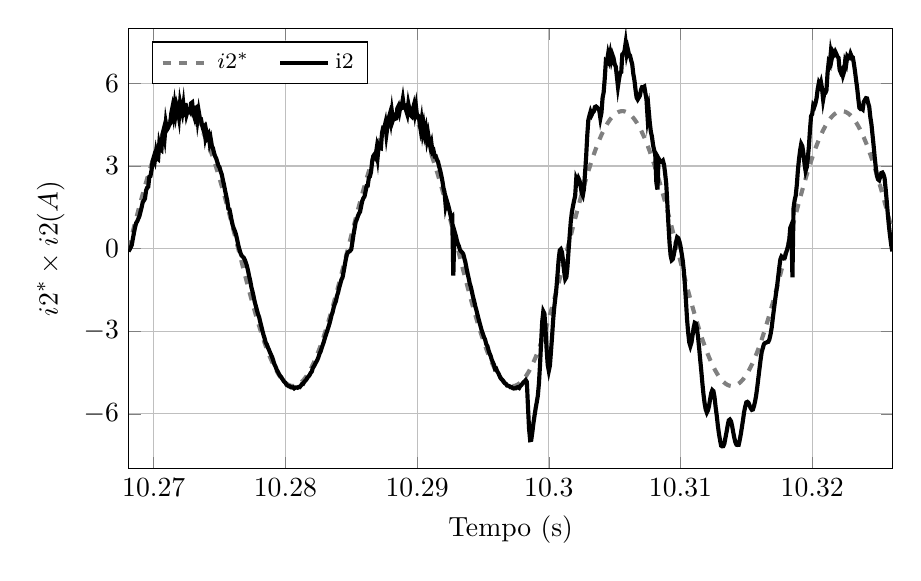
\begin{tikzpicture}

\begin{axis}[%
width=0.8\textwidth,
height=0.461611624834875\textwidth,
scale only axis,
xmin=10.2681,
xmax=10.3261,
xtick={10.27, 10.28, 10.29,  10.3, 10.31, 10.32},
xlabel={Tempo (s)},
xmajorgrids,
ymin=-8,
ymax=8,
ytick={-6, -3,  0,  3,  6},
ylabel={$\text{i2}^\text{*}\text{ }\times\text{ i2 (A)}$},
ymajorgrids,
legend style={at={(0.03,0.97)},anchor=north west,draw=black,fill=white,legend cell align=left},
scaled x ticks = false,
legend columns=-1,
legend style={/tikz/every even column/.append style={column sep=0.3cm}},
legend style={font=\footnotesize}
]
\addplot [color=gray,dashed,line width=1.5pt]
  table[row sep=crcr]{10.2680833456702	0.000309070768819114\\
10.2681666556704	0.157053337715448\\
10.2682499956706	0.313642611979031\\
10.2683333356708	0.469922358851122\\
10.268416675671	0.625738349089441\\
10.2684999856713	0.780936811123516\\
10.2685833256715	0.935364582808655\\
10.2686666656717	1.0888692625785\\
10.2687500056719	1.24129935984695\\
10.2688333456721	1.39250444451113\\
10.2689166556723	1.54233529540767\\
10.2689999956725	1.69064404757604\\
10.2690833356727	1.83728433818338\\
10.2691666756729	1.98211145096696\\
10.2692499856731	2.12498245905166\\
10.2693333256733	2.26575636600151\\
10.2694166656735	2.4042942449662\\
10.2695000056738	2.54045937578506\\
10.269583345674	2.67411737991341\\
10.2696666556742	2.80513635303789\\
10.2697499956744	2.93338699525013\\
10.2698333356746	3.05874273865016\\
10.2699166756748	3.18107987225364\\
10.269999985675	3.30027766407962\\
10.2700833256752	3.41621848029852\\
10.2701666656754	3.52878790132241\\
10.2702500056756	3.63787483472342\\
10.2703333456758	3.74337162486851\\
10.270416655676	3.84517415916259\\
10.2704999956763	3.94318197079508\\
10.2705833356765	4.03729833788853\\
10.2706666756767	4.12743037895141\\
10.2707499856769	4.21348914454097\\
10.2708333256771	4.29538970504559\\
10.2709166656773	4.3730512345\\
10.2710000056775	4.44639709035084\\
10.2710833456777	4.51535488909353\\
10.2711666556779	4.57985657770609\\
10.2712499956781	4.63983850080923\\
10.2713333356783	4.69524146348657\\
10.2714166756785	4.74601078970282\\
10.2714999856788	4.79209637626246\\
10.271583325679	4.83345274225553\\
10.2716666656792	4.87003907394182\\
10.2717500056794	4.90181926502907\\
10.2718333456796	4.92876195230555\\
10.2719166556798	4.95084054659175\\
10.27199999568	4.96803325898068\\
10.2720833356802	4.98032312234093\\
10.2721666756804	4.98769800806111\\
10.2722499856806	4.99015063801943\\
10.2723333256808	4.9876785917662\\
10.272416665681	4.98028430891263\\
10.2725000056813	4.96797508672318\\
10.2725833456815	4.95076307291404\\
10.2726666556817	4.9286652536648\\
10.2727499956819	4.90170343685516\\
10.2728333356821	4.86990423054316\\
10.2729166756823	4.83329901670629\\
10.2729999856825	4.79192392027119\\
10.2730833256827	4.74581977346277\\
10.2731666656829	4.6950320755077\\
10.2732500056831	4.6396109477322\\
10.2733333456833	4.57961108409831\\
10.2734166556835	4.51509169722756\\
10.2734999956838	4.44611645996527\\
10.273583335684	4.37275344254314\\
10.2736666756842	4.29507504540214\\
10.2737499856844	4.21315792774203\\
10.2738333256846	4.12708293186795\\
10.2739166656848	4.03693500340888\\
10.274000005685	3.94280310748652\\
10.2740833456852	3.84478014091745\\
10.2741666556854	3.74296284053523\\
10.2742499956856	3.63745168772278\\
10.2743333356858	3.52835080924942\\
10.274416675686	3.41576787451028\\
10.2744999856863	3.29981398926965\\
10.2745833256865	3.18060358601299\\
10.2746666656867	3.05825431101585\\
10.2747500056869	2.93288690824126\\
10.2748333456871	2.80462510017996\\
10.2749166556873	2.67359546575128\\
10.2749999956875	2.53992731538499\\
10.2750833356877	2.40375256340756\\
10.2751666756879	2.26520559785861\\
10.2752499856881	2.12442314786616\\
10.2753333256883	1.98154414871148\\
10.2754166656885	1.83670960471674\\
10.2755000056888	1.69006245009079\\
10.275583345689	1.54174740787031\\
10.2756666556892	1.39191084709568\\
10.2757499956894	1.24070063836241\\
10.2758333356896	1.08826600789067\\
10.2759166756898	0.934757390257092\\
10.27599998569	0.780326279933957\\
10.2760833256902	0.625125081782461\\
10.2761666656904	0.469306960647512\\
10.2762500056906	0.313025690202519\\
10.2763333456908	0.156435501193346\\
10.276416655691	-0.000309070768817629\\
10.2764999956913	-0.157053337715447\\
10.2765833356915	-0.313642611979031\\
10.2766666756917	-0.469922358851123\\
10.2767499856919	-0.625738349089442\\
10.2768333256921	-0.780936811123517\\
10.2769166656923	-0.935364582808657\\
10.2770000056925	-1.0888692625785\\
10.2770833456927	-1.24129935984696\\
10.2771666556929	-1.39250444451113\\
10.2772499956931	-1.54233529540767\\
10.2773333356933	-1.69064404757604\\
10.2774166756935	-1.83728433818339\\
10.2774999856937	-1.98211145096697\\
10.277583325694	-2.12498245905166\\
10.2776666656942	-2.26575636600152\\
10.2777500056944	-2.4042942449662\\
10.2778333456946	-2.54045937578507\\
10.2779166556948	-2.67411737991342\\
10.277999995695	-2.8051363530379\\
10.2780833356952	-2.93338699525014\\
10.2781666756954	-3.05874273865018\\
10.2782499856956	-3.18107987225365\\
10.2783333256958	-3.30027766407964\\
10.278416665696	-3.41621848029853\\
10.2785000056963	-3.52878790132242\\
10.2785833456965	-3.63787483472343\\
10.2786666556967	-3.74337162486853\\
10.2787499956969	-3.84517415916261\\
10.2788333356971	-3.9431819707951\\
10.2789166756973	-4.03729833788854\\
10.2789999856975	-4.12743037895142\\
10.2790833256977	-4.21348914454099\\
10.2791666656979	-4.2953897050456\\
10.2792500056981	-4.37305123450002\\
10.2793333456983	-4.44639709035086\\
10.2794166556985	-4.51535488909355\\
10.2794999956988	-4.57985657770611\\
10.279583335699	-4.63983850080925\\
10.2796666756992	-4.69524146348659\\
10.2797499856994	-4.74601078970284\\
10.2798333256996	-4.79209637626248\\
10.2799166656998	-4.83345274225555\\
10.2800000057	-4.87003907394184\\
10.2800833457002	-4.90181926502909\\
10.2801666557004	-4.92876195230557\\
10.2802499957006	-4.95084054659177\\
10.2803333357008	-4.9680332589807\\
10.280416675701	-4.98032312234094\\
10.2804999857012	-4.98769800806113\\
10.2805833257015	-4.99015063801945\\
10.2806666657017	-4.98767859176622\\
10.2807500057019	-4.98028430891265\\
10.2808333457021	-4.9679750867232\\
10.2809166557023	-4.95076307291406\\
10.2809999957025	-4.92866525366482\\
10.2810833357027	-4.90170343685517\\
10.2811666757029	-4.86990423054318\\
10.2812499857031	-4.83329901670631\\
10.2813333257033	-4.79192392027121\\
10.2814166657035	-4.74581977346279\\
10.2815000057038	-4.69503207550772\\
10.281583345704	-4.63961094773222\\
10.2816666557042	-4.57961108409833\\
10.2817499957044	-4.51509169722758\\
10.2818333357046	-4.44611645996529\\
10.2819166757048	-4.37275344254316\\
10.281999985705	-4.29507504540216\\
10.2820833257052	-4.21315792774204\\
10.2821666657054	-4.12708293186797\\
10.2822500057056	-4.0369350034089\\
10.2823333457058	-3.94280310748653\\
10.282416655706	-3.84478014091747\\
10.2824999957063	-3.74296284053525\\
10.2825833357065	-3.6374516877228\\
10.2826666757067	-3.52835080924944\\
10.2827499857069	-3.4157678745103\\
10.2828333257071	-3.29981398926967\\
10.2829166657073	-3.180603586013\\
10.2830000057075	-3.05825431101587\\
10.2830833457077	-2.93288690824127\\
10.2831666557079	-2.80462510017998\\
10.2832499957081	-2.67359546575129\\
10.2833333357083	-2.539927315385\\
10.2834166757085	-2.40375256340757\\
10.2834999857087	-2.26520559785862\\
10.283583325709	-2.12442314786617\\
10.2836666657092	-1.98154414871149\\
10.2837500057094	-1.83670960471675\\
10.2838333457096	-1.6900624500908\\
10.2839166557098	-1.54174740787032\\
10.28399999571	-1.39191084709569\\
10.2840833357102	-1.24070063836241\\
10.2841666757104	-1.08826600789068\\
10.2842499857106	-0.934757390257098\\
10.2843333257108	-0.780326279933963\\
10.284416665711	-0.625125081782466\\
10.2845000057113	-0.469306960647516\\
10.2845833457115	-0.313025690202523\\
10.2846666557117	-0.156435501193349\\
10.2847499957119	0.000309070768815339\\
10.2848333357121	0.157053337715446\\
10.2849166757123	0.31364261197903\\
10.2849999857125	0.469922358851122\\
10.2850833257127	0.625738349089443\\
10.2851666657129	0.780936811123518\\
10.2852500057131	0.935364582808659\\
10.2853333457133	1.0888692625785\\
10.2854166557135	1.24129935984696\\
10.2854999957137	1.39250444451113\\
10.285583335714	1.54233529540768\\
10.2856666757142	1.69064404757605\\
10.2857499857144	1.83728433818339\\
10.2858333257146	1.98211145096698\\
10.2859166657148	2.12498245905167\\
10.286000005715	2.26575636600152\\
10.2860833457152	2.40429424496621\\
10.2861666557154	2.54045937578508\\
10.2862499957156	2.67411737991343\\
10.2863333357158	2.80513635303791\\
10.286416675716	2.93338699525015\\
10.2864999857162	3.05874273865019\\
10.2865833257165	3.18107987225366\\
10.2866666657167	3.30027766407965\\
10.2867500057169	3.41621848029854\\
10.2868333457171	3.52878790132244\\
10.2869166557173	3.63787483472345\\
10.2869999957175	3.74337162486854\\
10.2870833357177	3.84517415916262\\
10.2871666757179	3.94318197079511\\
10.2872499857181	4.03729833788856\\
10.2873333257183	4.12743037895144\\
10.2874166657185	4.21348914454101\\
10.2875000057188	4.29538970504562\\
10.287583345719	4.37305123450004\\
10.2876666557192	4.44639709035088\\
10.2877499957194	4.51535488909357\\
10.2878333357196	4.57985657770613\\
10.2879166757198	4.63983850080927\\
10.28799998572	4.69524146348661\\
10.2880833257202	4.74601078970286\\
10.2881666657204	4.7920963762625\\
10.2882500057206	4.83345274225557\\
10.2883333457208	4.87003907394186\\
10.288416655721	4.90181926502911\\
10.2884999957212	4.92876195230559\\
10.2885833357215	4.95084054659179\\
10.2886666757217	4.96803325898072\\
10.2887499857219	4.98032312234097\\
10.2888333257221	4.98769800806116\\
10.2889166657223	4.99015063801947\\
10.2890000057225	4.98767859176624\\
10.2890833457227	4.98028430891268\\
10.2891666557229	4.96797508672323\\
10.2892499957231	4.95076307291408\\
10.2893333357233	4.92866525366484\\
10.2894166757235	4.9017034368552\\
10.2894999857238	4.8699042305432\\
10.289583325724	4.83329901670633\\
10.2896666657242	4.79192392027123\\
10.2897500057244	4.74581977346281\\
10.2898333457246	4.69503207550774\\
10.2899166557248	4.63961094773224\\
10.289999995725	4.57961108409835\\
10.2900833357252	4.51509169722759\\
10.2901666757254	4.44611645996531\\
10.2902499857256	4.37275344254318\\
10.2903333257258	4.29507504540218\\
10.290416665726	4.21315792774206\\
10.2905000057262	4.12708293186799\\
10.2905833457265	4.03693500340892\\
10.2906666557267	3.94280310748655\\
10.2907499957269	3.84478014091748\\
10.2908333357271	3.74296284053526\\
10.2909166757273	3.63745168772282\\
10.2909999857275	3.52835080924945\\
10.2910833257277	3.41576787451031\\
10.2911666657279	3.29981398926968\\
10.2912500057281	3.18060358601302\\
10.2913333457283	3.05825431101588\\
10.2914166557285	2.93288690824129\\
10.2914999957287	2.80462510017999\\
10.291583335729	2.6735954657513\\
10.2916666757292	2.53992731538501\\
10.2917499857294	2.40375256340758\\
10.2918333257296	2.26520559785863\\
10.2919166657298	2.12442314786618\\
10.29200000573	1.9815441487115\\
10.2920833457302	1.83670960471676\\
10.2921666557304	1.69006245009081\\
10.2922499957306	1.54174740787033\\
10.2923333357308	1.3919108470957\\
10.292416675731	1.24070063836242\\
10.2924999857313	1.08826600789068\\
10.2925833257315	0.934757390257102\\
10.2926666657317	0.780326279933967\\
10.2927500057319	0.62512508178247\\
10.2928333457321	0.469306960647519\\
10.2929166557323	0.313025690202525\\
10.2929999957325	0.156435501193351\\
10.2930833357327	-0.000309070768814229\\
10.2931666757329	-0.157053337715445\\
10.2932499857331	-0.31364261197903\\
10.2933333257333	-0.469922358851123\\
10.2934166657335	-0.625738349089444\\
10.2935000057337	-0.78093681112352\\
10.293583345734	-0.935364582808662\\
10.2936666557342	-1.08886926257851\\
10.2937499957344	-1.24129935984696\\
10.2938333357346	-1.39250444451114\\
10.2939166757348	-1.54233529540768\\
10.293999985735	-1.69064404757606\\
10.2940833257352	-1.8372843381834\\
10.2941666657354	-1.98211145096698\\
10.2942500057356	-2.12498245905168\\
10.2943333457358	-2.26575636600153\\
10.294416655736	-2.40429424496622\\
10.2944999957363	-2.54045937578509\\
10.2945833357365	-2.67411737991344\\
10.2946666757367	-2.80513635303792\\
10.2947499857369	-2.93338699525016\\
10.2948333257371	-3.0587427386502\\
10.2949166657373	-3.18107987225367\\
10.2950000057375	-3.30027766407966\\
10.2950833457377	-3.41621848029855\\
10.2951666557379	-3.52878790132245\\
10.2952499957381	-3.63787483472346\\
10.2953333357383	-3.74337162486856\\
10.2954166757385	-3.84517415916264\\
10.2954999857388	-3.94318197079513\\
10.295583325739	-4.03729833788857\\
10.2956666657392	-4.12743037895146\\
10.2957500057394	-4.21348914454102\\
10.2958333457396	-4.29538970504564\\
10.2959166557398	-4.37305123450006\\
10.29599999574	-4.4463970903509\\
10.2960833357402	-4.51535488909359\\
10.2961666757404	-4.57985657770615\\
10.2962499857406	-4.63983850080929\\
10.2963333257408	-4.69524146348663\\
10.296416665741	-4.74601078970288\\
10.2965000057412	-4.79209637626252\\
10.2965833457415	-4.83345274225559\\
10.2966666557417	-4.87003907394188\\
10.2967499957419	-4.90181926502913\\
10.2968333357421	-4.92876195230561\\
10.2969166757423	-4.95084054659181\\
10.2969999857425	-4.96803325898074\\
10.2970833257427	-4.98032312234099\\
10.2971666657429	-4.98769800806118\\
10.2972500057431	-4.99015063801949\\
10.2973333457433	-4.98767859176626\\
10.2974166557435	-4.9802843089127\\
10.2974999957438	-4.96797508672325\\
10.297583335744	-4.9507630729141\\
10.2976666757442	-4.92866525366486\\
10.2977499857444	-4.90170343685522\\
10.2978333257446	-4.86990423054323\\
10.2979166657448	-4.83329901670635\\
10.298000005745	-4.79192392027125\\
10.2980833457452	-4.74581977346283\\
10.2981666557454	-4.69503207550776\\
10.2982499957456	-4.63961094773226\\
10.2983333357458	-4.57961108409837\\
10.298416675746	-4.51509169722762\\
10.2984999857463	-4.44611645996533\\
10.2985833257465	-4.3727534425432\\
10.2986666657467	-4.2950750454022\\
10.2987500057469	-4.21315792774208\\
10.2988333457471	-4.127082931868\\
10.2989166557473	-4.03693500340894\\
10.2989999957475	-3.94280310748657\\
10.2990833357477	-3.8447801409175\\
10.2991666757479	-3.74296284053528\\
10.2992499857481	-3.63745168772283\\
10.2993333257483	-3.52835080924947\\
10.2994166657485	-3.41576787451033\\
10.2995000057488	-3.2998139892697\\
10.299583345749	-3.18060358601303\\
10.2996666557492	-3.05825431101589\\
10.2997499957494	-2.9328869082413\\
10.2998333357496	-2.80462510018\\
10.2999166757498	-2.67359546575132\\
10.29999998575	-2.53992731538503\\
10.3000833257502	-2.40375256340759\\
10.3001666657504	-2.26520559785864\\
10.3002500057506	-2.12442314786619\\
10.3003333457508	-1.98154414871151\\
10.300416655751	-1.83670960471677\\
10.3004999957513	-1.69006245009082\\
10.3005833357515	-1.54174740787034\\
10.3006666757517	-1.39191084709571\\
10.3007499857519	-1.24070063836243\\
10.3008333257521	-1.08826600789069\\
10.3009166657523	-0.934757390257109\\
10.3010000057525	-0.780326279933972\\
10.3010833457527	-0.625125081782474\\
10.3011666557529	-0.469306960647523\\
10.3012499957531	-0.313025690202528\\
10.3013333357533	-0.156435501193353\\
10.3014166757535	0.000309070768812411\\
10.3014999857538	0.157053337715444\\
10.301583325754	0.31364261197903\\
10.3016666657542	0.469922358851123\\
10.3017500057544	0.625738349089445\\
10.3018333457546	0.780936811123522\\
10.3019166557548	0.935364582808664\\
10.301999995755	1.08886926257851\\
10.3020833357552	1.24129935984697\\
10.3021666757554	1.39250444451114\\
10.3022499857556	1.54233529540769\\
10.3023333257558	1.69064404757606\\
10.302416665756	1.83728433818341\\
10.3025000057563	1.98211145096699\\
10.3025833457565	2.12498245905169\\
10.3026666557567	2.26575636600154\\
10.3027499957569	2.40429424496623\\
10.3028333357571	2.5404593757851\\
10.3029166757573	2.67411737991345\\
10.3029999857575	2.80513635303793\\
10.3030833257577	2.93338699525017\\
10.3031666657579	3.05874273865021\\
10.3032500057581	3.18107987225369\\
10.3033333457583	3.30027766407968\\
10.3034166557585	3.41621848029857\\
10.3034999957588	3.52878790132246\\
10.303583335759	3.63787483472348\\
10.3036666757592	3.74337162486857\\
10.3037499857594	3.84517415916265\\
10.3038333257596	3.94318197079515\\
10.3039166657598	4.03729833788859\\
10.30400000576	4.12743037895148\\
10.3040833457602	4.21348914454104\\
10.3041666557604	4.29538970504566\\
10.3042499957606	4.37305123450008\\
10.3043333357608	4.44639709035092\\
10.304416675761	4.51535488909361\\
10.3044999857613	4.57985657770616\\
10.3045833257615	4.63983850080931\\
10.3046666657617	4.69524146348665\\
10.3047500057619	4.7460107897029\\
10.3048333457621	4.79209637626254\\
10.3049166557623	4.83345274225561\\
10.3049999957625	4.87003907394191\\
10.3050833357627	4.90181926502916\\
10.3051666757629	4.92876195230564\\
10.3052499857631	4.95084054659183\\
10.3053333257633	4.96803325898077\\
10.3054166657635	4.98032312234101\\
10.3055000057638	4.9876980080612\\
10.305583345764	4.99015063801951\\
10.3056666557642	4.98767859176629\\
10.3057499957644	4.98028430891272\\
10.3058333357646	4.96797508672327\\
10.3059166757648	4.95076307291413\\
10.305999985765	4.92866525366488\\
10.3060833257652	4.90170343685524\\
10.3061666657654	4.86990423054325\\
10.3062500057656	4.83329901670638\\
10.3063333457658	4.79192392027127\\
10.306416655766	4.74581977346285\\
10.3064999957663	4.69503207550778\\
10.3065833357665	4.63961094773228\\
10.3066666757667	4.57961108409839\\
10.3067499857669	4.51509169722764\\
10.3068333257671	4.44611645996535\\
10.3069166657673	4.37275344254322\\
10.3070000057675	4.29507504540222\\
10.3070833457677	4.2131579277421\\
10.3071666557679	4.12708293186802\\
10.3072499957681	4.03693500340895\\
10.3073333357683	3.94280310748659\\
10.3074166757685	3.84478014091752\\
10.3074999857688	3.7429628405353\\
10.307583325769	3.63745168772285\\
10.3076666657692	3.52835080924948\\
10.3077500057694	3.41576787451034\\
10.3078333457696	3.29981398926971\\
10.3079166557698	3.18060358601305\\
10.30799999577	3.05825431101591\\
10.3080833357702	2.93288690824131\\
10.3081666757704	2.80462510018002\\
10.3082499857706	2.67359546575133\\
10.3083333257708	2.53992731538504\\
10.308416665771	2.40375256340761\\
10.3085000057713	2.26520559785865\\
10.3085833457715	2.1244231478662\\
10.3086666557717	1.98154414871152\\
10.3087499957719	1.83670960471678\\
10.3088333357721	1.69006245009083\\
10.3089166757723	1.54174740787034\\
10.3089999857725	1.39191084709572\\
10.3090833257727	1.24070063836244\\
10.3091666657729	1.0882660078907\\
10.3092500057731	0.934757390257115\\
10.3093333457733	0.780326279933977\\
10.3094166557735	0.625125081782479\\
10.3094999957738	0.469306960647527\\
10.309583335774	0.313025690202531\\
10.3096666757742	0.156435501193356\\
10.3097499857744	-0.000309070768810635\\
10.3098333257746	-0.157053337715443\\
10.3099166657748	-0.313642611979029\\
10.310000005775	-0.469922358851124\\
10.3100833457752	-0.625738349089446\\
10.3101666557754	-0.780936811123524\\
10.3102499957756	-0.935364582808666\\
10.3103333357758	-1.08886926257851\\
10.310416675776	-1.24129935984697\\
10.3104999857763	-1.39250444451115\\
10.3105833257765	-1.54233529540769\\
10.3106666657767	-1.69064404757607\\
10.3107500057769	-1.83728433818341\\
10.3108333457771	-1.982111450967\\
10.3109166557773	-2.1249824590517\\
10.3109999957775	-2.26575636600155\\
10.3110833357777	-2.40429424496624\\
10.3111666757779	-2.54045937578511\\
10.3112499857781	-2.67411737991346\\
10.3113333257783	-2.80513635303794\\
10.3114166657785	-2.93338699525019\\
10.3115000057788	-3.05874273865022\\
10.311583345779	-3.1810798722537\\
10.3116666557792	-3.30027766407969\\
10.3117499957794	-3.41621848029858\\
10.3118333357796	-3.52878790132248\\
10.3119166757798	-3.63787483472349\\
10.31199998578	-3.74337162486859\\
10.3120833257802	-3.84517415916267\\
10.3121666657804	-3.94318197079516\\
10.3122500057806	-4.03729833788861\\
10.3123333457808	-4.12743037895149\\
10.312416655781	-4.21348914454106\\
10.3124999957813	-4.29538970504568\\
10.3125833357815	-4.37305123450009\\
10.3126666757817	-4.44639709035093\\
10.3127499857819	-4.51535488909363\\
10.3128333257821	-4.57985657770618\\
10.3129166657823	-4.63983850080933\\
10.3130000057825	-4.69524146348667\\
10.3130833457827	-4.74601078970292\\
10.3131666557829	-4.79209637626256\\
10.3132499957831	-4.83345274225564\\
10.3133333357833	-4.87003907394192\\
10.3134166757835	-4.90181926502918\\
10.3134999857838	-4.92876195230566\\
10.313583325784	-4.95084054659185\\
10.3136666657842	-4.96803325898079\\
10.3137500057844	-4.98032312234103\\
10.3138333457846	-4.98769800806122\\
10.3139166557848	-4.99015063801953\\
10.313999995785	-4.98767859176631\\
10.3140833357852	-4.98028430891274\\
10.3141666757854	-4.96797508672329\\
10.3142499857856	-4.95076307291415\\
10.3143333257858	-4.9286652536649\\
10.314416665786	-4.90170343685526\\
10.3145000057863	-4.86990423054327\\
10.3145833457865	-4.8332990167064\\
10.3146666557867	-4.7919239202713\\
10.3147499957869	-4.74581977346287\\
10.3148333357871	-4.69503207550781\\
10.3149166757873	-4.6396109477323\\
10.3149999857875	-4.57961108409841\\
10.3150833257877	-4.51509169722766\\
10.3151666657879	-4.44611645996537\\
10.3152500057881	-4.37275344254324\\
10.3153333457883	-4.29507504540224\\
10.3154166557885	-4.21315792774212\\
10.3154999957888	-4.12708293186804\\
10.315583335789	-4.03693500340897\\
10.3156666757892	-3.94280310748661\\
10.3157499857894	-3.84478014091754\\
10.3158333257896	-3.74296284053532\\
10.3159166657898	-3.63745168772287\\
10.31600000579	-3.5283508092495\\
10.3160833457902	-3.41576787451036\\
10.3161666557904	-3.29981398926973\\
10.3162499957906	-3.18060358601306\\
10.3163333357908	-3.05825431101592\\
10.316416675791	-2.93288690824133\\
10.3164999857913	-2.80462510018003\\
10.3165833257915	-2.67359546575134\\
10.3166666657917	-2.53992731538505\\
10.3167500057919	-2.40375256340762\\
10.3168333457921	-2.26520559785866\\
10.3169166557923	-2.12442314786621\\
10.3169999957925	-1.98154414871153\\
10.3170833357927	-1.83670960471679\\
10.3171666757929	-1.69006245009084\\
10.3172499857931	-1.54174740787035\\
10.3173333257933	-1.39191084709572\\
10.3174166657935	-1.24070063836244\\
10.3175000057938	-1.0882660078907\\
10.317583345794	-0.93475739025712\\
10.3176666557942	-0.780326279933982\\
10.3177499957944	-0.625125081782483\\
10.3178333357946	-0.46930696064753\\
10.3179166757948	-0.313025690202534\\
10.317999985795	-0.156435501193358\\
10.3180833257952	0.000309070768808983\\
10.3181666657954	0.157053337715442\\
10.3182500057956	0.313642611979029\\
10.3183333457958	0.469922358851124\\
10.318416655796	0.625738349089447\\
10.3184999957963	0.780936811123526\\
10.3185833357965	0.935364582808669\\
10.3186666757967	1.08886926257851\\
10.3187499857969	1.24129935984697\\
10.3188333257971	1.39250444451115\\
10.3189166657973	1.5423352954077\\
10.3190000057975	1.69064404757607\\
10.3190833457977	1.83728433818342\\
10.3191666557979	1.98211145096701\\
10.3192499957981	2.1249824590517\\
10.3193333357983	2.26575636600156\\
10.3194166757985	2.40429424496625\\
10.3194999857988	2.54045937578512\\
10.319583325799	2.67411737991347\\
10.3196666657992	2.80513635303795\\
10.3197500057994	2.9333869952502\\
10.3198333457996	3.05874273865024\\
10.3199166557998	3.18107987225371\\
10.3199999958	3.3002776640797\\
10.3200833358002	3.4162184802986\\
10.3201666758004	3.52878790132249\\
10.3202499858006	3.63787483472351\\
10.3203333258008	3.7433716248686\\
10.320416665801	3.84517415916268\\
10.3205000058013	3.94318197079518\\
10.3205833458015	4.03729833788862\\
10.3206666558017	4.12743037895151\\
10.3207499958019	4.21348914454108\\
10.3208333358021	4.29538970504569\\
10.3209166758023	4.37305123450011\\
10.3209999858025	4.44639709035095\\
10.3210833258027	4.51535488909364\\
10.3211666658029	4.5798565777062\\
10.3212500058031	4.63983850080935\\
10.3213333458033	4.69524146348669\\
10.3214166558035	4.74601078970294\\
10.3214999958038	4.79209637626258\\
10.321583335804	4.83345274225565\\
10.3216666758042	4.87003907394195\\
10.3217499858044	4.9018192650292\\
10.3218333258046	4.92876195230568\\
10.3219166658048	4.95084054659188\\
10.322000005805	4.96803325898081\\
10.3220833458052	4.98032312234105\\
10.3221666558054	4.98769800806124\\
10.3222499958056	4.99015063801955\\
10.3223333358058	4.98767859176633\\
10.322416675806	4.98028430891276\\
10.3224999858063	4.96797508672331\\
10.3225833258065	4.95076307291417\\
10.3226666658067	4.92866525366492\\
10.3227500058069	4.90170343685528\\
10.3228333458071	4.86990423054329\\
10.3229166558073	4.83329901670642\\
10.3229999958075	4.79192392027132\\
10.3230833358077	4.74581977346289\\
10.3231666758079	4.69503207550783\\
10.3232499858081	4.63961094773232\\
10.3233333258083	4.57961108409843\\
10.3234166658085	4.51509169722768\\
10.3235000058088	4.44611645996539\\
10.323583345809	4.37275344254326\\
10.3236666558092	4.29507504540226\\
10.3237499958094	4.21315792774214\\
10.3238333358096	4.12708293186806\\
10.3239166758098	4.03693500340899\\
10.32399998581	3.94280310748662\\
10.3240833258102	3.84478014091756\\
10.3241666658104	3.74296284053534\\
10.3242500058106	3.63745168772289\\
10.3243333458108	3.52835080924952\\
10.324416655811	3.41576787451038\\
10.3244999958113	3.29981398926975\\
10.3245833358115	3.18060358601308\\
10.3246666758117	3.05825431101594\\
10.3247499858119	2.93288690824134\\
10.3248333258121	2.80462510018004\\
10.3249166658123	2.67359546575136\\
10.3250000058125	2.53992731538507\\
10.3250833458127	2.40375256340763\\
10.3251666558129	2.26520559785868\\
10.3252499958131	2.12442314786622\\
10.3253333358133	1.98154414871154\\
10.3254166758135	1.8367096047168\\
10.3254999858138	1.69006245009084\\
10.325583325814	1.54174740787036\\
10.3256666658142	1.39191084709573\\
10.3257500058144	1.24070063836245\\
10.3258333458146	1.08826600789071\\
10.3259166558148	0.934757390257126\\
10.325999995815	0.780326279933988\\
10.3260833358152	0.625125081782488\\
};
\addlegendentry{$\text{i2}^\text{*}$};

\addplot [color=black,solid,line width=1.5pt]
  table[row sep=crcr]{10.2680833456702	-0.101673057810471\\
10.2681666556704	-0.0358588488260956\\
10.2682499956706	0.0427178113301544\\
10.2683333356708	0.131304237111404\\
10.268416675671	0.362780067189529\\
10.2684999856713	0.576238319142654\\
10.2685833256715	0.775933143361404\\
10.2686666656717	0.932836219533279\\
10.2687500056719	0.992394325002029\\
10.2688333456721	1.08973929570515\\
10.2689166556723	1.18157889531453\\
10.2689999956725	1.3454888074239\\
10.2690833356727	1.50214163945515\\
10.2691666756729	1.69032523320515\\
10.2692499856731	1.74162528203328\\
10.2693333256733	1.8109429089864\\
10.2694166656735	2.10472953008015\\
10.2695000056738	2.21308524297078\\
10.269583345674	2.2453667371114\\
10.2696666556742	2.60721976445515\\
10.2697499956744	2.63049246953328\\
10.2698333356746	2.84269950078328\\
10.2699166756748	3.18002860234578\\
10.269999985675	3.31365897343953\\
10.2700833256752	3.19304129765828\\
10.2701666656754	3.4915825574239\\
10.2702500056756	3.27962577031453\\
10.2703333456758	3.24759452031453\\
10.270416655676	3.78011405156453\\
10.2704999956763	3.60719535039265\\
10.2705833356765	3.57316214726765\\
10.2706666756767	4.15347830937703\\
10.2707499856769	4.31188285039265\\
10.2708333256771	4.05838553593953\\
10.2709166656773	4.55286795781453\\
10.2710000056775	4.31188285039265\\
10.2710833456777	4.37394339726765\\
10.2711666556779	4.4805474011739\\
10.2712499956781	4.54110648320515\\
10.2713333356783	4.9089653699239\\
10.2714166756785	5.11266410039265\\
10.2714999856788	4.8569145886739\\
10.271583325679	5.20350272343953\\
10.2716666656792	4.89970633672078\\
10.2717500056794	5.17497489140828\\
10.2718333456796	5.01882254765828\\
10.2719166556798	4.76832816289265\\
10.27199999568	5.28257987187703\\
10.2720833356802	5.0701225964864\\
10.2721666756804	4.9109673230489\\
10.2722499856806	5.20875785039265\\
10.2723333256808	4.7778374402364\\
10.272416665681	5.2793266980489\\
10.2725000056813	4.87518241093953\\
10.2725833456815	5.01757132695515\\
10.2726666556817	5.04760062383015\\
10.2727499956819	4.98328787968953\\
10.2728333356821	5.27181937383015\\
10.2729166756823	5.30259940312703\\
10.2729999856825	4.9199761121114\\
10.2730833256827	4.78559500859578\\
10.2731666656829	5.09965140508015\\
10.2732500056831	5.12792899297078\\
10.2733333456833	4.69550711797078\\
10.2734166556835	4.98028495000203\\
10.2734999956838	4.74105155156453\\
10.273583335684	4.71502616093953\\
10.2736666756842	4.4895561902364\\
10.2737499856844	4.35067069218953\\
10.2738333256846	4.40872733281453\\
10.2739166656848	4.05938651250203\\
10.274000005685	4.24857108281453\\
10.2740833456852	4.05688407109578\\
10.2741666556854	4.1332085339864\\
10.2742499956856	3.8319145886739\\
10.2743333356858	3.9680474011739\\
10.274416675686	3.72130667851765\\
10.2744999856863	3.63922660039265\\
10.2745833256865	3.46380545781453\\
10.2746666656867	3.3454399792989\\
10.2747500056869	3.26461112187703\\
10.2748333456871	3.13048026250203\\
10.2749166556873	3.0031059949239\\
10.2749999956875	2.94529959843953\\
10.2750833356877	2.80215995000203\\
10.2751666756879	2.68654715703328\\
10.2752499856881	2.49435965703328\\
10.2753333256883	2.31668631718953\\
10.2754166656885	2.11048514531453\\
10.2755000056888	1.92155081914265\\
10.275583345689	1.73611991093953\\
10.2756666556892	1.44683768437703\\
10.2757499956894	1.4255669324239\\
10.2758333356896	1.23588187383015\\
10.2759166756898	1.01466605351765\\
10.27599998569	0.845000526173904\\
10.2760833256902	0.725383826955154\\
10.2761666656904	0.632293006642654\\
10.2762500056906	0.502666541798904\\
10.2763333456908	0.328746864064529\\
10.276416655691	0.133055946095779\\
10.2764999956913	-0.0180915148417206\\
10.2765833356915	-0.154224327341721\\
10.2766666756917	-0.250067833201096\\
10.2767499856919	-0.290857628122971\\
10.2768333256921	-0.329395225779221\\
10.2769166656923	-0.406970909372971\\
10.2770000056925	-0.518329551951096\\
10.2770833456927	-0.645203331247971\\
10.2771666556929	-0.815369346872971\\
10.2772499956931	-1.01231148554485\\
10.2773333356933	-1.1829779894511\\
10.2774166756935	-1.40794747187297\\
10.2774999856937	-1.55809395624797\\
10.277583325694	-1.74002144648235\\
10.2776666656942	-1.93045723749797\\
10.2777500056944	-2.08135445429485\\
10.2778333456946	-2.22924874140422\\
10.2779166556948	-2.3791449816386\\
10.277999995695	-2.4822455675761\\
10.2780833356952	-2.65591500116985\\
10.2781666756954	-2.80931465937297\\
10.2782499856956	-2.97697823359172\\
10.2783333256958	-3.13212960077922\\
10.278416665696	-3.25524971796672\\
10.2785000056963	-3.41190254999797\\
10.2785833456965	-3.47646553827922\\
10.2786666556967	-3.58357003046672\\
10.2787499956969	-3.67565987421672\\
10.2788333356971	-3.7735053332011\\
10.2789166756973	-3.85933907343547\\
10.2789999856975	-3.95192940546672\\
10.2790833256977	-4.07555001093547\\
10.2791666656979	-4.20467598749797\\
10.2792500056981	-4.2820014269511\\
10.2793333456983	-4.39035713984172\\
10.2794166556985	-4.46442940546672\\
10.2794999956988	-4.54325630976359\\
10.279583335699	-4.61107247187297\\
10.2796666756992	-4.65486519648235\\
10.2797499856994	-4.72092964960734\\
10.2798333256996	-4.78023751093547\\
10.2799166656998	-4.83904488398234\\
10.2800000057	-4.86832344843547\\
10.2800833457002	-4.94564888788859\\
10.2801666557004	-4.96917183710734\\
10.2802499957006	-4.99694893671672\\
10.2803333357008	-4.9997016222636\\
10.280416675701	-5.0347358019511\\
10.2804999857012	-5.04249337031047\\
10.2805833257015	-5.03498604609172\\
10.2806666657017	-5.07377388788859\\
10.2807500057019	-5.0447455675761\\
10.2808333457021	-5.04174263788859\\
10.2809166557023	-5.05300362421672\\
10.2809999957025	-5.02397530390422\\
10.2810833357027	-5.03073189570109\\
10.2811666757029	-4.97843087031047\\
10.2812499857031	-4.92337715937297\\
10.2813333257033	-4.91987374140422\\
10.2814166657035	-4.84855416132609\\
10.2815000057038	-4.80125801874797\\
10.281583345704	-4.76297066523234\\
10.2816666557042	-4.68589546991984\\
10.2817499957044	-4.64460518671672\\
10.2818333357046	-4.5943061144511\\
10.2819166757048	-4.51072457148234\\
10.281999985705	-4.46743233515422\\
10.2820833257052	-4.33280098749797\\
10.2821666657054	-4.27224190546672\\
10.2822500057056	-4.19541695429484\\
10.2823333457058	-4.11709053827922\\
10.282416655706	-4.04927437616985\\
10.2824999957063	-3.9496772082011\\
10.2825833357065	-3.8255561144511\\
10.2826666757067	-3.74322579218547\\
10.2827499857069	-3.61510079218547\\
10.2828333257071	-3.4962348253886\\
10.2829166657073	-3.38362496210735\\
10.2830000057075	-3.24073555781047\\
10.2830833457077	-3.12362129999797\\
10.2831666557079	-2.99649727656047\\
10.2832499957081	-2.87237618281047\\
10.2833333357083	-2.7424994738261\\
10.2834166757085	-2.59485543085735\\
10.2834999857087	-2.42443917109172\\
10.283583325709	-2.30632393671672\\
10.2836666657092	-2.13140328241985\\
10.2837500057094	-2.01053536249797\\
10.2838333457096	-1.91018746210735\\
10.2839166557098	-1.71524727656047\\
10.28399999571	-1.59613106562297\\
10.2840833357102	-1.41995919062297\\
10.2841666757104	-1.28232491327922\\
10.2842499857106	-1.1309272082011\\
10.2843333257108	-1.0508490832011\\
10.284416665711	-0.848651817576096\\
10.2845000057113	-0.618927696482346\\
10.2845833457115	-0.396961143747971\\
10.2846666557117	-0.211780479685471\\
10.2847499957119	-0.133954551951096\\
10.2848333357121	-0.111182335154221\\
10.2849166757123	-0.0809027941385956\\
10.2849999857125	-0.0276007921854706\\
10.2850833257127	0.229650184377029\\
10.2851666657129	0.500664588673904\\
10.2852500057131	0.726134559377029\\
10.2853333457133	0.966619178517654\\
10.2854166557135	1.05345389531453\\
10.2854999957137	1.17407157109578\\
10.285583335714	1.27091605351765\\
10.2856666757142	1.33622977422078\\
10.2857499857144	1.53817679570515\\
10.2858333257146	1.72410819218953\\
10.2859166657148	1.8289604871114\\
10.286000005715	1.88526541875203\\
10.2860833457152	2.06669242070515\\
10.2861666557154	2.2713921277364\\
10.2862499957156	2.28215262578328\\
10.2863333357158	2.56843192265828\\
10.286416675716	2.61722953008015\\
10.2864999857162	2.78138968633015\\
10.2865833257165	3.1412407605489\\
10.2866666657167	3.3514458386739\\
10.2867500057169	3.40900199101765\\
10.2868333457171	3.32917411015828\\
10.2869166557173	3.59318167851765\\
10.2869999957175	3.31616141484578\\
10.2870833357177	3.74057547734578\\
10.2871666757179	3.66099784062703\\
10.2872499857181	3.64498221562703\\
10.2873333257183	4.19051444218953\\
10.2874166657185	4.38370291875203\\
10.2875000057188	4.37494437383015\\
10.287583345719	4.54335868047078\\
10.2876666557192	4.13971488164265\\
10.2877499957194	4.43525321172078\\
10.2878333357196	4.72253348515828\\
10.2879166757198	4.86417166875203\\
10.28799998572	4.62443778203328\\
10.2880833257202	4.97528006718953\\
10.2881666657204	4.67048270390828\\
10.2882500057206	4.78909842656453\\
10.2883333457208	4.71002127812703\\
10.288416655721	4.72528617070515\\
10.2884999957212	5.09364554570515\\
10.2885833357215	5.1742241589864\\
10.2886666757217	4.97878348515828\\
10.2887499857219	5.19299246953328\\
10.2888333257221	5.19274222539265\\
10.2889166657223	5.42797171758015\\
10.2890000057225	5.14144217656453\\
10.2890833457227	5.16446463750203\\
10.2891666557229	5.01782157109578\\
10.2892499957231	4.88544242070515\\
10.2893333357233	5.25004813359578\\
10.2894166757235	5.05085379765828\\
10.2894999857238	4.8398979871114\\
10.289583325724	4.80111014531453\\
10.2896666657242	5.0410942761739\\
10.2897500057244	5.19649588750203\\
10.2898333457246	4.91171805547078\\
10.2899166557248	5.14769828008015\\
10.289999995725	4.77933890508015\\
10.2900833357252	4.79410330937703\\
10.2901666757254	4.66447684453328\\
10.2902499857256	4.38795706914265\\
10.2903333257258	4.65046317265828\\
10.290416665726	4.25057303593953\\
10.2905000057262	4.47479178593953\\
10.2905833457265	4.1672417371114\\
10.2906666557267	4.34191214726765\\
10.2907499957269	3.96854788945515\\
10.2908333357271	4.16974417851765\\
10.2909166757273	3.9109917371114\\
10.2909999857275	3.7037895886739\\
10.2910833257277	3.8379204480489\\
10.2911666657279	3.50509574101765\\
10.2912500057281	3.54813773320515\\
10.2913333457283	3.34619071172078\\
10.2914166557285	3.35194632695515\\
10.2914999957287	3.23283011601765\\
10.291583335729	3.15650565312703\\
10.2916666757292	2.98458792851765\\
10.2917499857294	2.84144828008015\\
10.2918333257296	2.66127249883015\\
10.2919166657298	2.46232840703328\\
10.29200000573	2.20382620976765\\
10.2920833457302	2.04592215703328\\
10.2921666557304	1.5677056042989\\
10.2922499957306	1.7498833386739\\
10.2923333357308	1.61600272343953\\
10.292416675731	1.4706108777364\\
10.2924999857313	1.29418875859578\\
10.2925833257315	1.1022515027364\\
10.2926666657317	1.1492974011739\\
10.2927500057319	-0.980280235544846\\
10.2928333457321	0.638048621877029\\
10.2929166557323	0.500164100392654\\
10.2929999957325	0.336003944142654\\
10.2930833357327	0.185857459767654\\
10.2931666757329	0.0975212781270294\\
10.2932499857331	-0.0423651964823456\\
10.2933333257333	-0.0971686632792206\\
10.2934166657335	-0.135706260935471\\
10.2935000057337	-0.194013145701096\\
10.293583345734	-0.345160606638596\\
10.2936666557342	-0.499060753122971\\
10.2937499957344	-0.709516075388596\\
10.2938333357346	-0.90195381952922\\
10.2939166757348	-1.08137886835735\\
10.293999985735	-1.26931221796672\\
10.2940833257352	-1.39893868281047\\
10.2941666657354	-1.5793647082011\\
10.2942500057356	-1.76304390741985\\
10.2943333457358	-1.90918648554485\\
10.294416655736	-2.09236519648235\\
10.2944999957363	-2.23250191523235\\
10.2945833357365	-2.40041573359172\\
10.2946666757367	-2.55306465937297\\
10.2947499857369	-2.70271065546672\\
10.2948333257371	-2.85035469843547\\
10.2949166657373	-2.9937445910136\\
10.2950000057375	-3.10034859491985\\
10.2950833457377	-3.22246773554485\\
10.2951666557379	-3.30930245234172\\
10.2952499957381	-3.46945870234172\\
10.2953333357383	-3.53477242304485\\
10.2954166757385	-3.67816231562297\\
10.2954999857388	-3.80328438593547\\
10.295583325739	-3.8966254503886\\
10.2956666657392	-4.03551094843547\\
10.2957500057394	-4.12434761835735\\
10.2958333457396	-4.21618721796672\\
10.2959166557398	-4.37434151484172\\
10.29599999574	-4.35632393671672\\
10.2960833357402	-4.45692208124797\\
10.2961666757404	-4.52248604609172\\
10.2962499857406	-4.60857003046672\\
10.2963333257408	-4.69115059687297\\
10.296416665741	-4.74195015741985\\
10.2965000057412	-4.77873604609172\\
10.2965833457415	-4.84329903437297\\
10.2966666557417	-4.89309761835734\\
10.2967499957419	-4.91386788202922\\
10.2968333357421	-4.97317574335734\\
10.2969166757423	-4.97868111445109\\
10.2969999857425	-4.99569771601359\\
10.2970833257427	-5.03073189570109\\
10.2971666657429	-5.02622750116984\\
10.2972500057431	-5.06676705195109\\
10.2973333457433	-5.07952950312297\\
10.2974166557435	-5.07127144648234\\
10.2974999957438	-5.0697699816386\\
10.297583335744	-5.03673775507609\\
10.2976666757442	-5.03373482538859\\
10.2977499857444	-5.05875923945109\\
10.2978333257446	-4.98869088007609\\
10.2979166657448	-4.95490792109172\\
10.298000005745	-4.90285713984172\\
10.2980833457452	-4.84980538202922\\
10.2981666557454	-4.82002632929485\\
10.2982499957456	-4.77398140741984\\
10.2983333357458	-4.84329903437297\\
10.298416675746	-5.71990425898234\\
10.2984999857463	-6.53620064570109\\
10.2985833257465	-6.9546088488261\\
10.2986666657467	-6.94585030390422\\
10.2987500057469	-6.66582711054484\\
10.2988333457471	-6.3340033800761\\
10.2989166557473	-6.06424019648234\\
10.2989999957475	-5.80423653437297\\
10.2990833357477	-5.58151924921672\\
10.2991666757479	-5.34528878046672\\
10.2992499857481	-4.89685128046672\\
10.2993333257483	-4.2219428332011\\
10.2994166657485	-3.4041449816386\\
10.2995000057488	-2.64315254999797\\
10.299583345749	-2.28029854609172\\
10.2996666557492	-2.36087715937297\\
10.2997499957494	-2.91041329218547\\
10.2998333357496	-3.64412911249797\\
10.2999166757498	-4.21793892695109\\
10.29999998575	-4.43790352656047\\
10.3000833257502	-4.24796822382609\\
10.3001666657504	-3.72670967890422\\
10.3002500057506	-3.17742379023235\\
10.3003333457508	-2.57358467890422\\
10.300416655751	-2.12114327265422\\
10.3004999957513	-1.78206246210735\\
10.3005833357515	-1.40894844843547\\
10.3006666757517	-0.912964561716721\\
10.3007499857519	-0.389954307810471\\
10.3008333257521	-0.0648871691385956\\
10.3009166657523	-0.0243476183573456\\
10.3010000057525	-0.127197960154221\\
10.3010833457527	-0.442255333201096\\
10.3011666557529	-0.837140587107346\\
10.3012499957531	-1.1059027941386\\
10.3013333357533	-1.03933785273235\\
10.3014166757535	-0.667224815622971\\
10.3014999857538	-0.0731452257792206\\
10.301583325754	0.461376258595779\\
10.3016666657542	0.970122596486404\\
10.3017500057544	1.31520926640828\\
10.3018333457546	1.53992850468953\\
10.3019166557548	1.7348686902364\\
10.301999995755	1.90428397343953\\
10.3020833357552	2.52789237187703\\
10.3021666757554	2.4305474011739\\
10.3022499857556	2.55516898320515\\
10.3023333257558	2.4645806042989\\
10.302416665756	2.27489554570515\\
10.3025000057563	2.0131401746114\\
10.3025833457565	1.9270561902364\\
10.3026666557567	2.15653006718953\\
10.3027499957569	2.73234183476765\\
10.3028333357571	3.3174126355489\\
10.3029166757573	4.08366019414265\\
10.3029999857575	4.65621878789265\\
10.3030833257577	4.82238089726765\\
10.3031666657579	4.96577078984578\\
10.3032500057581	4.85215995000203\\
10.3033333457583	4.93449027226765\\
10.3034166557585	4.98028495000203\\
10.3034999957588	5.13693778203328\\
10.303583335759	5.15845877812703\\
10.3036666757592	5.12592703984578\\
10.3037499857594	5.06787039922078\\
10.3038333257596	5.00956351445515\\
10.3039166657598	4.7347954480489\\
10.30400000576	4.93924491093953\\
10.3040833457602	5.47201468633015\\
10.3041666557604	5.67846610234578\\
10.3042499957606	6.1832085339864\\
10.3043333357608	6.81357352422078\\
10.304416675761	6.77853934453328\\
10.3044999857613	7.04930350468953\\
10.3045833257615	6.87638480351765\\
10.3046666657617	7.0850884167989\\
10.3047500057619	6.85311209843953\\
10.3048333457621	7.02828299687703\\
10.3049166557623	6.91442191289265\\
10.3049999957625	6.69620902226765\\
10.3050833357627	6.60912406133015\\
10.3051666757629	6.26003348515828\\
10.3052499857631	5.88641898320515\\
10.3053333257633	6.15893485234578\\
10.3054166657635	6.37364432500203\\
10.3055000057638	6.40792777226765\\
10.305583345764	7.05230643437703\\
10.3056666557642	7.07958304570515\\
10.3057499957644	7.17692801640828\\
10.3058333357646	7.45494925664265\\
10.3059166757648	7.06281668828328\\
10.305999985765	7.2372368542989\\
10.3060833257652	7.05856253789265\\
10.3061666657654	7.01051566289265\\
10.3062500057656	6.83709647343953\\
10.3063333457658	6.6937065808614\\
10.306416655766	6.34461600468953\\
10.3064999957663	6.1191460339864\\
10.3065833357665	5.77831351445515\\
10.3066666757667	5.48602835820515\\
10.3067499857669	5.41270682500203\\
10.3068333257671	5.48077323125203\\
10.3069166657673	5.5515923230489\\
10.3070000057675	5.76204764531453\\
10.3070833457677	5.86214530156453\\
10.3071666557679	5.8598931042989\\
10.3072499957681	5.88316580937703\\
10.3073333357683	5.64818656133015\\
10.3074166757685	5.42096488164265\\
10.3074999857688	4.7748345105489\\
10.307583325769	5.0260796277364\\
10.3076666657692	4.57413870976765\\
10.3077500057694	4.24056327031453\\
10.3078333457696	4.06038748906453\\
10.3079166557698	3.7578423230489\\
10.30799999577	3.57391287968953\\
10.3080833357702	3.41500785039265\\
10.3081666757704	2.39901663945515\\
10.3082499857706	2.14401786015828\\
10.3083333257708	3.27562186406453\\
10.308416665771	3.20505301640828\\
10.3085000057713	3.15500418828328\\
10.3085833457715	3.14049002812703\\
10.3086666557717	3.18578421758015\\
10.3087499957719	3.04264456914265\\
10.3088333357721	2.7268364636739\\
10.3089166757723	2.3594780652364\\
10.3089999857725	1.63902518437703\\
10.3090833257727	0.887291785939529\\
10.3091666657729	0.209880897267654\\
10.3092500057731	-0.254572227732346\\
10.3093333457733	-0.419483116404221\\
10.3094166557735	-0.381446007029221\\
10.3094999957738	-0.206525352732346\\
10.309583335774	0.0184441296895294\\
10.3096666757742	0.250170203908279\\
10.3097499857744	0.412828895314529\\
10.3098333257746	0.380046912892654\\
10.3099166657748	0.264934608205154\\
10.310000005775	0.0885124890645294\\
10.3100833457752	-0.162982872263596\\
10.3101666557754	-0.421485069529221\\
10.3102499957756	-0.792597130076096\\
10.3103333357758	-1.30985176874797\\
10.310416675776	-1.91419136835735\\
10.3104999857763	-2.58109200312297\\
10.3105833257765	-3.05730660273235\\
10.3106666657767	-3.4061469347636\\
10.3107500057769	-3.53877632929485\\
10.3108333457771	-3.40864937616985\\
10.3109166557773	-3.15139839960735\\
10.3109999957775	-2.86887276484172\\
10.3110833357777	-2.69520333124797\\
10.3111666757779	-2.7184760363261\\
10.3112499857781	-2.90340645624797\\
10.3113333257783	-3.21571114374797\\
10.3114166657785	-3.6173529894511\\
10.3115000057788	-4.05202706171672\\
10.311583345779	-4.46342842890422\\
10.3116666557792	-4.91361763788859\\
10.3117499957794	-5.30975411249797\\
10.3118333357796	-5.62030709101359\\
10.3119166757798	-5.84102242304485\\
10.31199998578	-5.95313179804484\\
10.3120833257802	-5.87130196406047\\
10.3121666657804	-5.71239693476359\\
10.3122500057806	-5.47116158320109\\
10.3123333457808	-5.24719307734172\\
10.312416655781	-5.13658516718547\\
10.3124999957813	-5.17362129999797\\
10.3125833357815	-5.38732979609172\\
10.3126666757817	-5.74993355585734\\
10.3127499857819	-6.0537299425761\\
10.3128333257821	-6.41383126093547\\
10.3129166657823	-6.71012032343547\\
10.3130000057825	-6.94484932734172\\
10.3130833457827	-7.15430367304484\\
10.3131666557829	-7.17882759882609\\
10.3132499957831	-7.17157051874797\\
10.3133333357833	-7.07948067499797\\
10.3134166757835	-6.85851509882609\\
10.3134999857838	-6.65381539179484\\
10.313583325784	-6.41808541132609\\
10.3136666657842	-6.23615792109172\\
10.3137500057844	-6.20537789179484\\
10.3138333457846	-6.26368477656047\\
10.3139166557848	-6.43059761835734\\
10.313999995785	-6.65731880976359\\
10.3140833357852	-6.86502144648234\\
10.3141666757854	-7.03218453241985\\
10.3142499857856	-7.11901924921672\\
10.3143333257858	-7.12827828241984\\
10.314416665786	-7.12702706171672\\
10.3145000057863	-6.94334786249797\\
10.3145833457865	-6.72588570429484\\
10.3146666557867	-6.47539131952922\\
10.3147499957869	-6.21213448359172\\
10.3148333357871	-5.92685616327922\\
10.3149166757873	-5.73466866327922\\
10.3149999857875	-5.58302071406047\\
10.3150833257877	-5.56475289179484\\
10.3151666657879	-5.60103829218547\\
10.3152500057881	-5.70313790156047\\
10.3153333457883	-5.79447701288859\\
10.3154166557885	-5.85478585077922\\
10.3154999957888	-5.84102242304485\\
10.315583335789	-5.71114571406047\\
10.3156666757892	-5.54448311640422\\
10.3157499857894	-5.31275704218547\\
10.3158333257896	-5.01571724726359\\
10.3159166657898	-4.68289254023234\\
10.31600000579	-4.35156929804485\\
10.3160833457902	-4.03125679804485\\
10.3161666557904	-3.7534858019511\\
10.3162499957906	-3.61460030390422\\
10.3163333357908	-3.4712104113261\\
10.316416675791	-3.4271674425761\\
10.3164999857913	-3.41565621210735\\
10.3165833257915	-3.39288399531047\\
10.3166666657917	-3.3841254503886\\
10.3167500057919	-3.29478829218547\\
10.3168333457921	-3.12737496210735\\
10.3169166557923	-2.8966498644511\\
10.3169999957925	-2.56707833124797\\
10.3170833357927	-2.24576485468547\\
10.3171666757929	-1.93821480585735\\
10.3172499857931	-1.63817208124797\\
10.3173333257933	-1.3721625597636\\
10.3174166657935	-1.03433296991985\\
10.3175000057938	-0.692749717966721\\
10.317583345794	-0.390955284372971\\
10.3176666557942	-0.288605430857346\\
10.3177499957944	-0.325891807810471\\
10.3178333357946	-0.353668907419846\\
10.3179166757948	-0.330646446482346\\
10.317999985795	-0.174243858591721\\
10.3180833257952	-0.0596320421854706\\
10.3181666657954	0.0972710339864044\\
10.3182500057956	0.252922889455154\\
10.3183333457958	0.748156043752029\\
10.318416655796	0.851506873830154\\
10.3184999957963	-1.04008858515422\\
10.3185833357965	1.46310355351765\\
10.3186666757967	1.75038382695515\\
10.3187499857969	1.92430350468953\\
10.3188333257971	2.31093070195515\\
10.3189166657973	2.85120780156453\\
10.3190000057975	3.2493462292989\\
10.3190833457977	3.56715628789265\\
10.3191666557979	3.7968804089864\\
10.3192499957981	3.72005545781453\\
10.3193333357983	3.4615532605489\\
10.3194166757985	3.0821831433614\\
10.3194999857988	2.81667411015828\\
10.319583325799	2.94630057500203\\
10.3196666657992	3.26761405156453\\
10.3197500057994	3.7107964246114\\
10.3198333457996	4.31788870976765\\
10.3199166557998	4.8118706433614\\
10.3199999958	4.8829399792989\\
10.3200833358002	5.20650565312703\\
10.3201666758004	5.15195243047078\\
10.3202499858006	5.27582328008015\\
10.3203333258008	5.45975272343953\\
10.320416665801	5.78557059453328\\
10.3205000058013	6.00028006718953\\
10.3205833458015	5.91169364140828\\
10.3206666558017	6.03931815312703\\
10.3207499958019	5.80859305547078\\
10.3208333358021	5.41120536015828\\
10.3209166758023	5.6406792371114\\
10.3209999858025	5.65219046758015\\
10.3210833258027	5.75103690312703\\
10.3211666658029	6.37289359258015\\
10.3212500058031	6.75351493047078\\
10.3213333458033	6.68394705937703\\
10.3214166558035	7.12287528203328\\
10.3214999958038	6.92918631718953\\
10.321583335804	7.13638846562703\\
10.3216666758042	7.06782157109578\\
10.3217499858044	7.15290457890828\\
10.3218333258046	7.06957328008015\\
10.3219166658048	6.96947562383015\\
10.322000005805	6.92242972539265\\
10.3220833458052	6.49476248906453\\
10.3221666558054	6.39866873906453\\
10.3222499958056	6.4664849011739\\
10.3223333358058	6.2813042371114\\
10.322416675806	6.41118094609578\\
10.3224999858063	6.79005057500203\\
10.3225833258065	6.68945243047078\\
10.3226666658067	6.97272879765828\\
10.3227500058069	6.91617362187703\\
10.3228333458071	6.9099175183614\\
10.3229166558073	7.06832205937703\\
10.3229999958075	6.97047660039265\\
10.3230833358077	6.94269950078328\\
10.3231666758079	6.72098319218953\\
10.3232499858081	6.44070975468953\\
10.3233333258083	6.12239920781453\\
10.3234166658085	5.82135550664265\\
10.3235000058088	5.4464897839864\\
10.323583345809	5.11141287968953\\
10.3236666558092	5.0701225964864\\
10.3237499958094	5.0851372449239\\
10.3238333358096	5.0511040417989\\
10.3239166758098	5.32587210820515\\
10.32399998581	5.39393851445515\\
10.3240833258102	5.46075370000203\\
10.3241666658104	5.4514946667989\\
10.3242500058106	5.2823296277364\\
10.3243333458108	5.14169242070515\\
10.324416655811	4.76432425664265\\
10.3244999958113	4.51007620976765\\
10.3245833358115	4.11944510625203\\
10.3246666758117	3.72756278203328\\
10.3247499858119	3.30314871953328\\
10.3248333258121	2.9280327527364\\
10.3249166658123	2.64225394414265\\
10.3250000058125	2.5146294324239\\
10.3250833458127	2.48034598515828\\
10.3251666558129	2.6067192761739\\
10.3252499958131	2.74535453008015\\
10.3253333358133	2.76036917851765\\
10.3254166758135	2.68904959843953\\
10.3254999858138	2.54816214726765\\
10.325583325814	2.1352593152364\\
10.3256666658142	1.68807303593953\\
10.3257500058144	1.20610282109578\\
10.3258333458146	0.796202918752029\\
10.3259166558148	0.442357703908279\\
10.325999995815	0.133806678517654\\
10.3260833358152	-0.101172569529221\\
};
\addlegendentry{i2};

\end{axis}
\end{tikzpicture}%}}
    \end{figure}
    \end{small}
    \vfill
  }

  \frame{
    \frametitle{\insertsection}
    \vfill
    \begin{small}
    \begin{figure}[htb]
      \centering
      \raisebox{-0.5\height}{
        %\def\svgwidth{0.8\linewidth}
        \resizebox{0.9\linewidth}{!}{% This file was created by matlab2tikz v0.4.7 running on MATLAB 7.14.
% Copyright (c) 2008--2014, Nico Schlömer <nico.schloemer@gmail.com>
% All rights reserved.
% Minimal pgfplots version: 1.3
% 
% The latest updates can be retrieved from
%   http://www.mathworks.com/matlabcentral/fileexchange/22022-matlab2tikz
% where you can also make suggestions and rate matlab2tikz.
% 
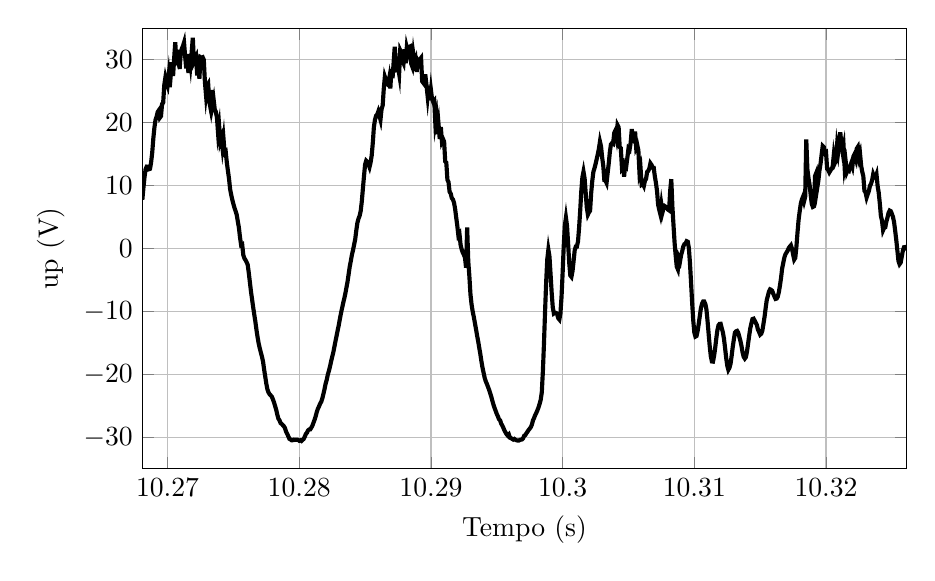
\begin{tikzpicture}

\begin{axis}[%
width=0.8\textwidth,
height=0.461611624834875\textwidth,
scale only axis,
xmin=10.2681,
xmax=10.3261,
xtick={10.27, 10.28, 10.29,  10.3, 10.31, 10.32},
xlabel={Tempo (s)},
xmajorgrids,
ymin=-35,
ymax=35,
ytick={-30, -20, -10,   0,  10,  20,  30},
ylabel={up (V)},
ymajorgrids,
scaled x ticks = false,
legend columns=-1,
legend style={/tikz/every even column/.append style={column sep=0.3cm}},
legend style={font=\footnotesize}
]
\addplot [color=black,solid,line width=1.5pt,forget plot]
  table[row sep=crcr]{10.2680833456702	7.75178374148825\\
10.2681666556704	9.66122776122889\\
10.2682499956706	11.3480305316769\\
10.2683333356708	12.6347569331264\\
10.268416675671	13.0145089376779\\
10.2684999856713	12.9962502065075\\
10.2685833256715	12.6083016629513\\
10.2686666656717	12.6681703354293\\
10.2687500056719	13.7091959356695\\
10.2688333456721	15.2048843303268\\
10.2689166556723	17.4299736956324\\
10.2689999956725	19.1872277238551\\
10.2690833356727	20.4340806640802\\
10.2691666756729	20.9373286251577\\
10.2692499856731	21.6924434573819\\
10.2693333256733	21.9469735208169\\
10.2694166656735	20.7975879802335\\
10.2695000056738	21.0380527423934\\
10.269583345674	22.9618302887242\\
10.2696666556742	23.1764661252038\\
10.2697499956744	25.9788927257931\\
10.2698333356746	27.1494365119501\\
10.2699166756748	26.4012765916794\\
10.269999985675	25.8898362020413\\
10.2700833256752	27.4898609710595\\
10.2701666656754	25.622361794351\\
10.2702500056756	27.7310086349226\\
10.2703333456758	29.5757065460887\\
10.270416655676	27.3957245832176\\
10.2704999956763	30.1765269011936\\
10.2705833356765	32.7711126167063\\
10.2706666756767	29.832105980089\\
10.2707499856769	29.5155920759201\\
10.2708333256771	31.560451791595\\
10.2709166656773	28.5300322664104\\
10.2710000056775	31.003633611871\\
10.2710833456777	31.7658005979907\\
10.2711666556779	32.1521053378452\\
10.2712499956781	32.7251516648173\\
10.2713333356783	30.5729190628843\\
10.2714166756785	28.6049737908159\\
10.2714999856788	30.5396296325426\\
10.271583325679	27.8933406814689\\
10.2716666656792	30.9057051329016\\
10.2717500056794	29.3834173111155\\
10.2718333456796	31.2719009685935\\
10.2719166556798	33.4959752134652\\
10.27199999568	29.6687290275569\\
10.2720833356802	30.0664664916033\\
10.2721666756804	30.450423053945\\
10.2722499856806	27.4990646375428\\
10.2723333256808	30.25868659286\\
10.272416665681	26.975378976366\\
10.2725000056813	30.4023132460389\\
10.2725833456815	30.2963692900291\\
10.2726666556817	30.3799490490278\\
10.2727499956819	30.0001055638667\\
10.2728333356821	26.5610166772863\\
10.2729166756823	24.4512126887033\\
10.2729999856825	25.9063707410884\\
10.2730833256827	26.1841649085971\\
10.2731666656829	23.3638549072387\\
10.2732500056831	22.4451612292773\\
10.2733333456833	25.186652000644\\
10.2734166556835	22.7430241704026\\
10.2734999956838	23.627107815129\\
10.273583335684	22.0965505902197\\
10.2736666756842	21.7200304362982\\
10.2737499856844	20.7894269027222\\
10.2738333256846	18.3736076565549\\
10.2739166656848	19.4784971472497\\
10.274000005685	17.0081763058158\\
10.2740833456852	17.563749639445\\
10.2741666556854	16.0354500441864\\
10.2742499956856	17.4039944376876\\
10.2743333356858	15.1758425515865\\
10.274416675686	15.3549606325307\\
10.2744999856863	13.6598551356748\\
10.2745833256865	12.3547185219862\\
10.2746666656867	11.0928207601823\\
10.2747500056869	9.4328193933959\\
10.2748333456871	8.5340097647061\\
10.2749166556873	7.7497996526146\\
10.2749999956875	7.07553651435069\\
10.2750833356877	6.45357503177898\\
10.2751666756879	5.94729946662756\\
10.2752499856881	5.37667514778839\\
10.2753333256883	4.33470274753117\\
10.2754166656885	3.31669016578943\\
10.2755000056888	1.80918222255009\\
10.275583345689	0.572337819914381\\
10.2756666556892	0.663129048198669\\
10.2757499956894	-1.01083390204897\\
10.2758333356896	-1.53777349247337\\
10.2759166756898	-1.82786076283258\\
10.27599998569	-2.14656221042063\\
10.2760833256902	-2.5544146870423\\
10.2761666656904	-3.83788375812394\\
10.2762500056906	-5.33802707277494\\
10.2763333456908	-6.8136665892565\\
10.276416655691	-8.05929679995035\\
10.2764999956913	-9.31785404008564\\
10.2765833356915	-10.480844981013\\
10.2766666756917	-11.5951689247489\\
10.2767499856919	-12.8972694434787\\
10.2768333256921	-14.0469593958444\\
10.2769166656923	-15.0646176413951\\
10.2770000056925	-15.8270742982203\\
10.2770833456927	-16.5080797904229\\
10.2771666556929	-17.1703749255302\\
10.2772499956931	-17.9441188501215\\
10.2773333356933	-19.2271639121648\\
10.2774166756935	-20.3319269940839\\
10.2774999856937	-21.477292698892\\
10.277583325694	-22.3667387672605\\
10.2776666656942	-22.8568246777814\\
10.2777500056944	-23.1371160055858\\
10.2778333456946	-23.3213169765294\\
10.2779166556948	-23.5119723871573\\
10.277999995695	-23.9555793359234\\
10.2780833356952	-24.4285378214247\\
10.2781666756954	-25.0176106564701\\
10.2782499856956	-25.6054928683531\\
10.2783333256958	-26.380097657594\\
10.278416665696	-27.0197850435188\\
10.2785000056963	-27.2836581000606\\
10.2785833456965	-27.7288202539283\\
10.2786666556967	-27.8516438862787\\
10.2787499956969	-28.0464439925193\\
10.2788333356971	-28.228688763933\\
10.2789166756973	-28.5143166162397\\
10.2789999856975	-29.0943933183585\\
10.2790833256977	-29.4214400631573\\
10.2791666656979	-29.8111131685673\\
10.2792500056981	-30.2196776480765\\
10.2793333456983	-30.3091432084591\\
10.2794166556985	-30.4464318861628\\
10.2794999956988	-30.4379902146459\\
10.279583335699	-30.3520567654333\\
10.2796666756992	-30.3920262884176\\
10.2797499856994	-30.347874892126\\
10.2798333256996	-30.3630287630577\\
10.2799166656998	-30.388606203282\\
10.2800000057	-30.52766348003\\
10.2800833457002	-30.466852188097\\
10.2801666557004	-30.5683501151778\\
10.2802499957006	-30.3789418574253\\
10.2803333357008	-30.2491868452081\\
10.280416675701	-29.8804547270008\\
10.2804999857012	-29.4645817933889\\
10.2805833257015	-29.2570311492256\\
10.2806666657017	-28.8791835990268\\
10.2807500057019	-28.7409335729663\\
10.2808333457021	-28.7221948695274\\
10.2809166557023	-28.4419919591389\\
10.2809999957025	-28.1200980965109\\
10.2810833357027	-27.6406088271232\\
10.2811666757029	-27.1663265916138\\
10.2812499857031	-26.615964820836\\
10.2813333257033	-25.9374864271454\\
10.2814166657035	-25.4178835864612\\
10.2815000057038	-25.0672398292295\\
10.281583345704	-24.6371458888471\\
10.2816666557042	-24.3414578242416\\
10.2817499957044	-23.8156542636383\\
10.2818333357046	-23.1044311815305\\
10.2819166757048	-22.3403808834177\\
10.281999985705	-21.4711775760497\\
10.2820833257052	-20.8781347200225\\
10.2821666657054	-20.0301307784085\\
10.2822500057056	-19.4314135363719\\
10.2823333457058	-18.7422766386242\\
10.282416655706	-17.9331864444213\\
10.2824999957063	-17.2059077504113\\
10.2825833357065	-16.5132404899906\\
10.2826666757067	-15.6161048265415\\
10.2827499857069	-14.7202149778765\\
10.2828333257071	-13.874643129194\\
10.2829166657073	-12.9855318237232\\
10.2830000057075	-12.1676207800214\\
10.2830833457077	-11.1921946435389\\
10.2831666557079	-10.2811162023939\\
10.2832499957081	-9.4800291098854\\
10.2833333357083	-8.66804907102587\\
10.2834166757085	-7.94186355086694\\
10.2834999857087	-7.14021346540318\\
10.283583325709	-6.19028803337425\\
10.2836666657092	-5.2649803006502\\
10.2837500057094	-4.05025025461594\\
10.2838333457096	-2.86787824789959\\
10.2839166557098	-1.95538128973827\\
10.28399999571	-0.963722008989586\\
10.2840833357102	-0.238911394218603\\
10.2841666757104	0.633577959707511\\
10.2842499857106	1.48994424916366\\
10.2843333257108	2.90876910462841\\
10.284416665711	4.11147450173345\\
10.2845000057113	4.76743128959649\\
10.2845833457115	5.20524745367739\\
10.2846666557117	5.9917337820864\\
10.2847499957119	7.50388702963892\\
10.2848333357121	9.54545169967292\\
10.2849166757123	11.5278643370938\\
10.2849999857125	13.3553739229399\\
10.2850833257127	13.952542428025\\
10.2851666657129	13.7865222833901\\
10.2852500057131	13.4002157606535\\
10.2853333457133	12.9324915269175\\
10.2854166557135	13.6679583495977\\
10.2854999957137	14.7804685765124\\
10.285583335714	16.7506496140727\\
10.2856666757142	19.3036421482042\\
10.2857499857144	20.4582668361124\\
10.2858333257146	21.0827898258789\\
10.2859166657148	21.262415831135\\
10.286000005715	21.7621235735637\\
10.2860833457152	21.1219099591396\\
10.2861666557154	20.4667268960453\\
10.2862499957156	22.1607117734045\\
10.2863333357158	22.7103477401477\\
10.286416675716	25.3654819576207\\
10.2864999857162	27.2833728845879\\
10.2865833257165	26.7538372803965\\
10.2866666657167	26.1386321430614\\
10.2867500057169	25.9934864215016\\
10.2868333457171	27.0179700360396\\
10.2869166557173	25.4397823323078\\
10.2869999957175	28.5087749590625\\
10.2870833357177	27.0503290569779\\
10.2871666757179	29.5936175032976\\
10.2872499857181	32.0531627129158\\
10.2873333257183	29.5939824177775\\
10.2874166657185	28.6441496940271\\
10.2875000057188	28.8565154244219\\
10.287583345719	27.7658239112382\\
10.2876666557192	31.4957583880408\\
10.2877499957194	31.1127788594189\\
10.2878333357196	29.8440785712196\\
10.2879166757198	29.4486766938689\\
10.28799998572	31.6542483760304\\
10.2880833257202	29.4591184261009\\
10.2881666657204	31.928172973721\\
10.2882500057206	31.2031518090974\\
10.2883333457208	32.0023222647377\\
10.288416655721	32.0958132362827\\
10.2884999957212	29.3726868021707\\
10.2885833357215	28.9032863479245\\
10.2886666757217	30.8188252259734\\
10.2887499857219	29.5611543021361\\
10.2888333257221	30.0386903308572\\
10.2889166657223	28.0390766223666\\
10.2890000057225	29.872284000365\\
10.2890833457227	29.5568795513248\\
10.2891666557229	30.0541514023529\\
10.2892499957231	30.2834310309791\\
10.2893333357233	26.5628070373543\\
10.2894166757235	26.3298762351669\\
10.2894999857238	27.3857017428559\\
10.289583325724	27.385091779419\\
10.2896666657242	25.8627026775424\\
10.2897500057244	24.1660335505588\\
10.2898333457246	25.8559055395108\\
10.2899166557248	23.5519536576332\\
10.289999995725	25.1744246082023\\
10.2900833357252	23.767234188881\\
10.2901666757254	23.3119429594453\\
10.2902499857256	23.5132247253276\\
10.2903333257258	19.8920234880931\\
10.290416665726	20.9153819570543\\
10.2905000057262	18.1501687878045\\
10.2905833457265	19.5477277646817\\
10.2906666557267	17.3968733268307\\
10.2907499957269	19.3036049797628\\
10.2908333357271	17.018008984048\\
10.2909166757273	17.4019019562604\\
10.2909999857275	16.9891291913391\\
10.2910833257277	13.8298077042659\\
10.2911666657279	13.6397614429734\\
10.2912500057281	10.926045109446\\
10.2913333457283	10.5574558546488\\
10.2914166557285	9.01316637126196\\
10.2914999957287	8.73647279299116\\
10.291583335729	8.01908814699881\\
10.2916666757292	7.8054802174819\\
10.2917499857294	7.29991493247398\\
10.2918333257296	6.34239009123344\\
10.2919166657298	4.95821639228315\\
10.29200000573	3.62571944528562\\
10.2920833457302	2.06385781222306\\
10.2921666557304	2.31688444363611\\
10.2922499957306	0.611339369465988\\
10.2923333357308	-0.139333732988894\\
10.292416675731	-0.626723130485677\\
10.2924999857313	-0.988219711298863\\
10.2925833257315	-1.42168053898559\\
10.2926666657317	-3.03597375342382\\
10.2927500057319	3.35921129749894\\
10.2928333457321	-2.03846408925625\\
10.2929166557323	-4.36038695631532\\
10.2929999957325	-7.26913971939011\\
10.2930833357327	-8.85471671621182\\
10.2931666757329	-9.95927739466485\\
10.2932499857331	-10.8113698550333\\
10.2933333257333	-11.7697895775044\\
10.2934166657335	-12.7434081787305\\
10.2935000057337	-13.7782492889357\\
10.293583345734	-14.6971954770186\\
10.2936666557342	-15.7308436276001\\
10.2937499957344	-16.7601427004402\\
10.2938333357346	-17.9192178092529\\
10.2939166757348	-18.9348266490966\\
10.293999985735	-19.7437468883819\\
10.2940833257352	-20.5665320782958\\
10.2941666657354	-21.1090889313318\\
10.2942500057356	-21.508680212303\\
10.2943333457358	-21.9738975574497\\
10.294416655736	-22.4348321066788\\
10.2944999957363	-22.9895161751341\\
10.2945833357365	-23.5399192530993\\
10.2946666757367	-24.1976733916295\\
10.2947499857369	-24.8075766893149\\
10.2948333257371	-25.3404308172514\\
10.2949166657373	-25.7891939314423\\
10.2950000057375	-26.2824640164233\\
10.2950833457377	-26.6511140145414\\
10.2951666557379	-27.1141015938716\\
10.2952499957381	-27.2728592369343\\
10.2953333357383	-27.8089646990196\\
10.2954166757385	-28.0980399539078\\
10.2954999857388	-28.4835109742355\\
10.295583325739	-28.9113577592939\\
10.2956666657392	-29.2132277850468\\
10.2957500057394	-29.5218647218686\\
10.2958333457396	-29.7088842893749\\
10.2959166557398	-29.5309690017775\\
10.29599999574	-30.0369540034806\\
10.2960833357402	-30.1197267185172\\
10.2961666757404	-30.2270840851175\\
10.2962499857406	-30.3403237342761\\
10.2963333257408	-30.2393148004148\\
10.296416665741	-30.3670983613989\\
10.2965000057412	-30.4541833650595\\
10.2965833457415	-30.4904449361833\\
10.2966666557417	-30.5027126620032\\
10.2967499957419	-30.3976544840118\\
10.2968333357421	-30.3399724050488\\
10.2969166757423	-30.3195687250405\\
10.2969999857425	-30.1195555745579\\
10.2970833257427	-29.7199535155094\\
10.2971666657429	-29.6234958391189\\
10.2972500057431	-29.3321134050384\\
10.2973333457433	-29.0729913508513\\
10.2974166557435	-28.8139980453465\\
10.2974999957438	-28.6058176951946\\
10.297583335744	-28.3705493520212\\
10.2976666757442	-27.9477151171889\\
10.2977499857444	-27.2669810287136\\
10.2978333257446	-26.9000776490106\\
10.2979166657448	-26.4304877284927\\
10.298000005745	-26.0940183492115\\
10.2980833457452	-25.6899661960115\\
10.2981666557454	-25.2383244028321\\
10.2982499957456	-24.6756416832002\\
10.2983333357458	-24.0340661895206\\
10.298416675746	-22.8356128079896\\
10.2984999857463	-19.4795204063554\\
10.2985833257465	-15.0344441196152\\
10.2986666657467	-9.91655300220308\\
10.2987500057469	-5.27668891954426\\
10.2988333457471	-1.69086594415417\\
10.2989166557473	-0.172604209703108\\
10.2989999957475	-1.25692213947509\\
10.2990833357477	-4.09054049503161\\
10.2991666757479	-6.98635753190671\\
10.2992499857481	-9.32554933420173\\
10.2993333257483	-10.2983994165005\\
10.2994166657485	-10.172974653796\\
10.2995000057488	-10.2240251165023\\
10.299583345749	-10.4299461911634\\
10.2996666557492	-11.0601014101719\\
10.2997499957494	-11.2676638407266\\
10.2998333357496	-10.2771618096754\\
10.2999166757498	-7.63350394691991\\
10.29999998575	-3.83180735839002\\
10.3000833257502	0.418263593684855\\
10.3001666657504	3.63636625243439\\
10.3002500057506	4.90329518592065\\
10.3003333457508	3.59553404171498\\
10.300416655751	0.742228623703633\\
10.3004999957513	-2.26996941525184\\
10.3005833357515	-4.27595041284556\\
10.3006666757517	-4.49491891298795\\
10.3007499857519	-3.59211305993486\\
10.3008333257521	-1.94899733410288\\
10.3009166657523	-0.26493929643475\\
10.3010000057525	0.319067529606601\\
10.3010833457527	0.327793254052953\\
10.3011666557529	1.13870091479881\\
10.3012499957531	3.340549856038\\
10.3013333357533	6.02964355345684\\
10.3014166757535	9.13078906333442\\
10.3014999857538	11.3331037050634\\
10.301583325754	12.2198314770899\\
10.3016666657542	11.1767585433403\\
10.3017500057544	8.86777801521933\\
10.3018333457546	6.53247551717979\\
10.3019166557548	5.39703815294851\\
10.301999995755	5.7627907134487\\
10.3020833357552	5.9940678603375\\
10.3021666757554	8.81185558988473\\
10.3022499857556	10.734906999379\\
10.3023333257558	12.1784096138758\\
10.302416665756	12.7478062333152\\
10.3025000057563	13.4346500788888\\
10.3025833457565	14.1875813572276\\
10.3026666557567	14.9690647913861\\
10.3027499957569	15.8083845249496\\
10.3028333357571	16.9858917567146\\
10.3029166757573	16.2302140845868\\
10.3029999857575	14.4758882882718\\
10.3030833257577	13.1906911878445\\
10.3031666657579	10.8630224943965\\
10.3032500057581	10.7968864388346\\
10.3033333457583	10.4241670794973\\
10.3034166557585	12.0032033961735\\
10.3034999957588	13.4989345933625\\
10.303583335759	15.3079802471481\\
10.3036666757592	16.5484453434889\\
10.3037499857594	16.7585340988732\\
10.3038333257596	16.6479137489521\\
10.3039166657598	18.361404713658\\
10.30400000576	18.7247225830336\\
10.3040833457602	17.7773598568904\\
10.3041666557604	19.6183335172243\\
10.3042499957606	19.2869433527549\\
10.3043333357608	16.1202810735309\\
10.304416675761	15.96340870721\\
10.3044999857613	12.9631099483023\\
10.3045833257615	13.3032896404028\\
10.3046666657617	11.4369073927902\\
10.3047500057619	13.3875127318959\\
10.3048333457621	13.1190086569691\\
10.3049166557623	14.4676153887877\\
10.3049999957625	15.9113544591575\\
10.3050833357627	15.7112592630402\\
10.3051666757629	16.8398451047272\\
10.3052499857631	18.9661988512482\\
10.3053333257633	17.3894853720658\\
10.3054166657635	17.1409161025855\\
10.3055000057638	18.5931786147043\\
10.305583345764	16.0547932295419\\
10.3056666557642	16.4465880219217\\
10.3057499957644	15.6036510339729\\
10.3058333357646	12.1069279292241\\
10.3059166757648	12.7715920098314\\
10.305999985765	10.1663089512932\\
10.3060833257652	10.2924188692325\\
10.3061666657654	9.93900102742903\\
10.3062500057656	10.7663046166134\\
10.3063333457658	11.0611691531976\\
10.306416655766	12.1818611408854\\
10.3064999957663	12.3338683240026\\
10.3065833357665	12.731110869818\\
10.3066666757667	13.5401076926219\\
10.3067499857669	13.2880041894591\\
10.3068333257671	12.8579169132832\\
10.3069166657673	12.8291981847223\\
10.3070000057675	11.4847125798808\\
10.3070833457677	10.4370157416955\\
10.3071666557679	9.16718026202298\\
10.3072499957681	6.98519094465949\\
10.3073333357683	6.16298626359239\\
10.3074166757685	5.47794111075667\\
10.3074999857688	6.96695732765204\\
10.307583325769	5.76831197711466\\
10.3076666657692	6.43892651488408\\
10.3077500057694	6.74644793496894\\
10.3078333457696	6.6311359084142\\
10.3079166557698	6.54179870763736\\
10.30799999577	6.18570538862901\\
10.3080833357702	6.06631990250919\\
10.3081666757704	9.19548574296807\\
10.3082499857706	11.0243298550871\\
10.3083333257708	6.68935185935782\\
10.308416665771	3.77901840603049\\
10.3085000057713	0.964669020179006\\
10.3085833457715	-1.12474855557491\\
10.3086666557717	-2.87983821117521\\
10.3087499957719	-3.28710610627824\\
10.3088333357721	-1.55201905304765\\
10.3089166757723	-1.99369173223571\\
10.3089999857725	-0.986481039062915\\
10.3090833257727	-0.373963890883565\\
10.3091666657729	0.370628163714961\\
10.3092500057731	0.710758031130515\\
10.3093333457733	0.790522233386169\\
10.3094166557735	1.16949714126077\\
10.3094999957738	1.09155900702318\\
10.309583335774	0.118279565346403\\
10.3096666757742	-2.24870370836378\\
10.3097499857744	-5.35141269253728\\
10.3098333257746	-8.56089918680538\\
10.3099166657748	-11.4067967545299\\
10.310000005775	-13.3327182527686\\
10.3100833457752	-13.9810529546545\\
10.3101666557754	-13.8840901823008\\
10.3102499957756	-13.1050804304962\\
10.3103333357758	-11.9486546014002\\
10.310416675776	-10.7111768585192\\
10.3104999857763	-9.46497915784533\\
10.3105833257765	-8.77522003558513\\
10.3106666657767	-8.41381100043259\\
10.3107500057769	-8.40928817516823\\
10.3108333457771	-8.77813262412092\\
10.3109166557773	-9.64302541174044\\
10.3109999957775	-11.4129434580933\\
10.3110833357777	-13.4729971950565\\
10.3111666757779	-15.4536561526127\\
10.3112499857781	-17.0952424518442\\
10.3113333257783	-17.9255669734927\\
10.3114166657785	-17.9531226492266\\
10.3115000057788	-17.0437042949449\\
10.311583345779	-15.7882946181105\\
10.3116666557792	-14.2786787674812\\
10.3117499957794	-12.9821328308049\\
10.3118333357796	-12.1882130190788\\
10.3119166757798	-11.9635030926654\\
10.31199998578	-11.9487913362668\\
10.3120833257802	-12.6595228367189\\
10.3121666657804	-13.2887095236209\\
10.3122500057806	-14.3059462550858\\
10.3123333457808	-15.7574425355417\\
10.312416655781	-17.3372841985391\\
10.3124999957813	-18.5832537585413\\
10.3125833357815	-19.2523449057671\\
10.3126666757817	-18.941667608683\\
10.3127499857819	-18.3097245728245\\
10.3128333257821	-17.0413009432298\\
10.3129166657823	-15.6122619302863\\
10.3130000057825	-14.4493073139699\\
10.3130833457827	-13.3485356052125\\
10.3131666557829	-13.1496934743173\\
10.3132499957831	-13.0743230339196\\
10.3133333357833	-13.3703094753757\\
10.3134166757835	-14.0201593348394\\
10.3134999857838	-14.6719286288744\\
10.313583325784	-15.504012048151\\
10.3136666657842	-16.5388377513194\\
10.3137500057844	-17.1958038705046\\
10.3138333457846	-17.4709410843046\\
10.3139166557848	-17.2369500124465\\
10.313999995785	-16.3283117199132\\
10.3140833357852	-15.0832718516018\\
10.3141666757854	-13.8086883812745\\
10.3142499857856	-12.6541201185357\\
10.3143333257858	-11.8809383244217\\
10.314416665786	-11.1948339583132\\
10.3145000057863	-11.1342625874123\\
10.3145833457865	-11.4426704287611\\
10.3146666557867	-11.8077287999097\\
10.3147499957869	-12.1604277631793\\
10.3148333357871	-12.8892065858969\\
10.3149166757873	-13.2570269731727\\
10.3149999857875	-13.6717550066819\\
10.3150833257877	-13.5157044061301\\
10.3151666657879	-13.035157260722\\
10.3152500057881	-11.9478822561085\\
10.3153333457883	-10.8296705933273\\
10.3154166557885	-9.43416766830777\\
10.3154999957888	-8.17102312095876\\
10.315583335789	-7.52527249751048\\
10.3156666757892	-6.83681088955173\\
10.3157499857894	-6.47639348038895\\
10.3158333257896	-6.56046811809775\\
10.3159166657898	-6.7233271443423\\
10.31600000579	-7.21045742469425\\
10.3160833457902	-7.60829728461936\\
10.3161666557904	-7.99574270378004\\
10.3162499957906	-7.94362668448506\\
10.3163333357908	-7.65081747763765\\
10.316416675791	-6.95037708397942\\
10.3164999857913	-5.8785637332301\\
10.3165833257915	-4.69336669697504\\
10.3166666657917	-3.17473865364255\\
10.3167500057919	-2.31274843262815\\
10.3168333457921	-1.45451034414228\\
10.3169166557923	-0.913230770221904\\
10.3169999957925	-0.629689860185823\\
10.3170833357927	-0.34862286871448\\
10.3171666757929	0.072557186524163\\
10.3172499857931	0.316664869099915\\
10.3173333257933	0.518374089407461\\
10.3174166657935	-0.0180343660608204\\
10.3175000057938	-0.933889031319452\\
10.317583345794	-1.75112624558607\\
10.3176666557942	-1.47723535538877\\
10.3177499957944	0.254206122962073\\
10.3178333357946	2.50819774323458\\
10.3179166757948	4.54298786313443\\
10.317999985795	5.92142747701373\\
10.3180833257952	7.09645281056789\\
10.3181666657954	7.78860692613354\\
10.3182500057956	8.2253658217938\\
10.3183333457958	7.51877991956893\\
10.318416655796	8.20212990477492\\
10.3184999957963	17.3511603361466\\
10.3185833357965	12.6410105833255\\
10.3186666757967	11.2157992477531\\
10.3187499857969	10.1688719508952\\
10.3188333257971	8.59131163109672\\
10.3189166657973	7.09990606270747\\
10.3190000057975	6.61917778208596\\
10.3190833457977	6.71082836900454\\
10.3191666557979	11.5246303350581\\
10.3192499957981	11.9649716317597\\
10.3193333357983	9.65892738965666\\
10.3194166757985	10.760027113533\\
10.3194999857988	12.3803933064856\\
10.319583325799	13.46519456801\\
10.3196666657992	14.9336470782602\\
10.3197500057994	16.291477850685\\
10.3198333457996	16.118280663926\\
10.3199166557998	15.2107607538959\\
10.3199999958	15.3143514273253\\
10.3200833358002	12.6661510302188\\
10.3201666758004	12.4747794864655\\
10.3202499858006	12.0942349311301\\
10.3203333258008	12.385588643804\\
10.320416665801	12.7154294328727\\
10.3205000058013	12.9334947928438\\
10.3205833458015	14.7106304643756\\
10.3206666558017	13.5598674945227\\
10.3207499958019	13.9397429221986\\
10.3208333358021	16.3069426088197\\
10.3209166758023	15.222450879517\\
10.3209999858025	16.619119161839\\
10.3210833258027	18.4506987481458\\
10.3211666658029	16.6484817431499\\
10.3212500058031	15.4707412965541\\
10.3213333458033	16.2860952106085\\
10.3214166558035	12.8270122885491\\
10.3214999958038	13.7144044045966\\
10.321583335804	12.1506911947804\\
10.3216666758042	12.5693190364372\\
10.3217499858044	12.4159477461355\\
10.3218333258046	13.0471566381755\\
10.3219166658048	13.5579635002919\\
10.322000005805	13.0372287842959\\
10.3220833458052	14.630917084624\\
10.3221666558054	14.9921055203839\\
10.3222499958056	14.3618272460883\\
10.3223333358058	15.8707777445531\\
10.322416675806	16.14496805646\\
10.3224999858063	14.4609373975744\\
10.3225833258065	15.0668705248541\\
10.3226666658067	13.1711878577127\\
10.3227500058069	12.2111289450899\\
10.3228333458071	11.4830049296226\\
10.3229166558073	9.16662656124313\\
10.3229999958075	8.93308205230722\\
10.3230833358077	8.116066005707\\
10.3231666758079	8.64074528372768\\
10.3232499858081	9.13463954864783\\
10.3233333258083	9.93729415154063\\
10.3234166658085	10.2792599323141\\
10.3235000058088	10.860229006729\\
10.323583345809	11.8066205879799\\
10.3236666558092	11.3772578386887\\
10.3237499958094	11.2809384814413\\
10.3238333358096	11.7653954105563\\
10.3239166758098	9.98074443687537\\
10.32399998581	8.89746148451607\\
10.3240833258102	7.21558004872801\\
10.3241666658104	5.17304626617812\\
10.3242500058106	4.45511448003057\\
10.3243333458108	2.91978825174416\\
10.324416655811	3.31221244000611\\
10.3244999958113	3.38159800844968\\
10.3245833358115	4.28324873877464\\
10.3246666758117	4.91470637124254\\
10.3247499858119	5.67488383879226\\
10.3248333258121	6.03589591182831\\
10.3249166658123	5.93973260299935\\
10.3250000058125	5.51967436229556\\
10.3250833458127	5.03089677062795\\
10.3251666558129	4.20986262793523\\
10.3252499958131	2.83807266251734\\
10.3253333358133	1.39716936050327\\
10.3254166758135	-0.261174843209325\\
10.3254999858138	-1.97442366932559\\
10.325583325814	-2.47722111252825\\
10.3256666658142	-2.2464441489292\\
10.3257500058144	-1.29058069415205\\
10.3258333458146	-0.350945012679667\\
10.3259166558148	0.20542321005887\\
10.325999995815	0.234801241919497\\
10.3260833358152	-0.2743788708142\\
};
\end{axis}
\end{tikzpicture}%}}
    \end{figure}
    \end{small}
    \vfill
  }

  \frame{
    \frametitle{\insertsection}
    \vfill
    \begin{small}
    \begin{figure}[htb]
      \centering
      \raisebox{-0.5\height}{
        %\def\svgwidth{0.8\linewidth}
        \resizebox{0.7\linewidth}{!}{% This file was created by matlab2tikz v0.4.7 running on MATLAB 7.14.
% Copyright (c) 2008--2014, Nico Schlömer <nico.schloemer@gmail.com>
% All rights reserved.
% Minimal pgfplots version: 1.3
% 
% The latest updates can be retrieved from
%   http://www.mathworks.com/matlabcentral/fileexchange/22022-matlab2tikz
% where you can also make suggestions and rate matlab2tikz.
% 
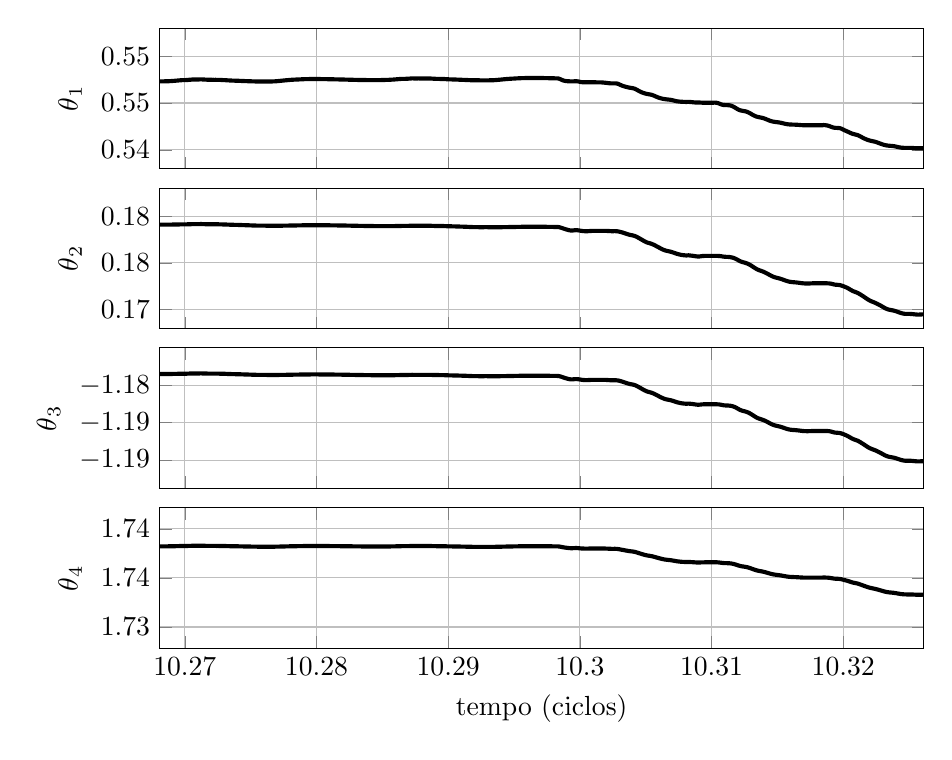
\begin{tikzpicture}

\begin{axis}[%
width=0.8\textwidth,
height=0.146941238746167\textwidth,
scale only axis,
xmin=10.2681,
xmax=10.3261,
xtick={10.27,10.28,10.29,10.3,10.31,10.32},
xticklabels={\empty},
xmajorgrids,
ymin=-1.195,
ymax=-1.18,
ytick={-1.192, -1.188, -1.184},
ylabel={$\theta{}_\text{3}$},
ymajorgrids,
name=plot2,
scaled x ticks = false,
legend columns=-1,
legend style={/tikz/every even column/.append style={column sep=0.3cm}},
legend style={font=\footnotesize}
]
\addplot [color=black,solid,line width=1.5pt,forget plot]
  table[row sep=crcr]{10.2680833456702	-1.18278439402264\\
10.2681666556704	-1.1827848754371\\
10.2682499956706	-1.18278535845101\\
10.2683333356708	-1.18278576770851\\
10.268416675671	-1.18278595571516\\
10.2684999856713	-1.18278600768181\\
10.2685833256715	-1.18278594826164\\
10.2686666656717	-1.1827857677017\\
10.2687500056719	-1.18278525877342\\
10.2688333456721	-1.18278436816531\\
10.2689166556723	-1.18278303468173\\
10.2689999956725	-1.18278153359931\\
10.2690833356727	-1.18277988292257\\
10.2691666756729	-1.18277826707253\\
10.2692499856731	-1.18277589252319\\
10.2693333256733	-1.18277274825542\\
10.2694166656735	-1.18277050075757\\
10.2695000056738	-1.18276788946194\\
10.269583345674	-1.18276418945938\\
10.2696666556742	-1.18276236051085\\
10.2697499956744	-1.18275942051498\\
10.2698333356746	-1.18275717735467\\
10.2699166756748	-1.1827571688289\\
10.269999985675	-1.18275732523367\\
10.2700833256752	-1.18275458669588\\
10.2701666656754	-1.18275410595448\\
10.2702500056756	-1.18274934721792\\
10.2703333456758	-1.18274257710663\\
10.270416655676	-1.18274169437259\\
10.2704999956763	-1.18273718208004\\
10.2705833356765	-1.18273082797992\\
10.2706666756767	-1.18273119195462\\
10.2707499856769	-1.18273253856188\\
10.2708333256771	-1.18272922049836\\
10.2709166656773	-1.18273182481751\\
10.2710000056775	-1.18272986932864\\
10.2710833456777	-1.18272776721187\\
10.2711666556779	-1.18272628974201\\
10.2712499956781	-1.18272482838945\\
10.2713333356783	-1.18272798652018\\
10.2714166756785	-1.18273338883721\\
10.2714999856788	-1.1827343567621\\
10.271583325679	-1.18274002037238\\
10.2716666656792	-1.18274047139541\\
10.2717500056794	-1.18274470809367\\
10.2718333456796	-1.18274609128131\\
10.2719166556798	-1.18274327467596\\
10.27199999568	-1.18274807415909\\
10.2720833356802	-1.18274941023199\\
10.2721666756804	-1.18274826255163\\
10.2722499856806	-1.18275150294803\\
10.2723333256808	-1.18274843805722\\
10.272416665681	-1.18275278968112\\
10.2725000056813	-1.18275146548463\\
10.2725833456815	-1.18275241873883\\
10.2726666556817	-1.18275409358011\\
10.2727499956819	-1.18275523232599\\
10.2728333356821	-1.182760822325\\
10.2729166756823	-1.18276731300232\\
10.2729999856825	-1.18276909791084\\
10.2730833256827	-1.18276965622121\\
10.2731666656829	-1.18277533073904\\
10.2732500056831	-1.18278205997359\\
10.2733333456833	-1.18278365407382\\
10.2734166556835	-1.18279011475893\\
10.2734999956838	-1.18279415634802\\
10.273583335684	-1.18279885037918\\
10.2736666756842	-1.18280149801211\\
10.2737499856844	-1.18280335697911\\
10.2738333256846	-1.18280711271493\\
10.2739166656848	-1.182807403559\\
10.274000005685	-1.18281136327589\\
10.2740833456852	-1.18281404741253\\
10.2741666556854	-1.1828189520539\\
10.2742499956856	-1.18282137106826\\
10.2743333356858	-1.18282684190207\\
10.274416675686	-1.18283059451389\\
10.2744999856863	-1.18283475904697\\
10.2745833256865	-1.18283820031965\\
10.2746666656867	-1.18284165171409\\
10.2747500056869	-1.18284557307375\\
10.2748333456871	-1.18284935476947\\
10.2749166556873	-1.18285311736486\\
10.2749999956875	-1.18285766659562\\
10.2750833356877	-1.1828620529778\\
10.2751666756879	-1.18286662181389\\
10.2752499856881	-1.1828705623008\\
10.2753333256883	-1.18287406301151\\
10.2754166656885	-1.18287684386335\\
10.2755000056888	-1.18287911220153\\
10.275583345689	-1.1828809308943\\
10.2756666556892	-1.18288141700905\\
10.2757499956894	-1.18288295513088\\
10.2758333356896	-1.18288408336607\\
10.2759166756898	-1.18288465067694\\
10.27599998569	-1.18288507446511\\
10.2760833256902	-1.18288566855228\\
10.2761666656904	-1.18288652628421\\
10.2762500056906	-1.18288740481853\\
10.2763333456908	-1.18288810625523\\
10.276416655691	-1.18288857620874\\
10.2764999956913	-1.18288898160475\\
10.2765833356915	-1.18288933444767\\
10.2766666756917	-1.18288965823008\\
10.2767499856919	-1.1828899040024\\
10.2768333256921	-1.1828899281905\\
10.2769166656923	-1.1828896644205\\
10.2770000056925	-1.18288913168955\\
10.2770833456927	-1.18288833895621\\
10.2771666556929	-1.18288732372765\\
10.2772499956931	-1.18288613153673\\
10.2773333356933	-1.18288468700986\\
10.2774166756935	-1.18288315758509\\
10.2774999856937	-1.18288131842298\\
10.277583325694	-1.18287931562995\\
10.2776666656942	-1.1828772890804\\
10.2777500056944	-1.18287506908471\\
10.2778333456946	-1.18287267221499\\
10.2779166556948	-1.18287017288597\\
10.277999995695	-1.18286720883163\\
10.2780833356952	-1.18286448271355\\
10.2781666756954	-1.18286189656779\\
10.2782499856956	-1.18285967206733\\
10.2783333256958	-1.18285775273454\\
10.278416665696	-1.18285583226938\\
10.2785000056963	-1.18285438053246\\
10.2785833456965	-1.18285230386648\\
10.2786666556967	-1.18285018240254\\
10.2787499956969	-1.18284788164862\\
10.2788333356971	-1.18284553976026\\
10.2789166756973	-1.18284305259058\\
10.2789999856975	-1.18284057598659\\
10.2790833256977	-1.1828386164759\\
10.2791666656979	-1.182837321647\\
10.2792500056981	-1.1828360126111\\
10.2793333456983	-1.18283520078821\\
10.2794166556985	-1.18283445780007\\
10.2794999956988	-1.18283392060265\\
10.279583335699	-1.18283349650841\\
10.2796666756992	-1.18283289846421\\
10.2797499856994	-1.18283252675307\\
10.2798333256996	-1.18283235158708\\
10.2799166656998	-1.18283243522206\\
10.2800000057	-1.18283241029806\\
10.2800833457002	-1.18283305785524\\
10.2801666557004	-1.18283365263281\\
10.2802499957006	-1.18283432972987\\
10.2803333357008	-1.18283479312216\\
10.280416675701	-1.18283558673795\\
10.2804999857012	-1.18283638150091\\
10.2805833257015	-1.1828370282371\\
10.2806666657017	-1.18283826413241\\
10.2807500057019	-1.18283918303372\\
10.2808333457021	-1.18284022947689\\
10.2809166557023	-1.18284167118798\\
10.2809999957025	-1.18284300631741\\
10.2810833357027	-1.18284480453051\\
10.2811666757029	-1.18284630758392\\
10.2812499857031	-1.18284754864004\\
10.2813333257033	-1.18284930105227\\
10.2814166657035	-1.18285069636981\\
10.2815000057038	-1.1828521295948\\
10.281583345704	-1.18285378105827\\
10.2816666557042	-1.18285519192394\\
10.2817499957044	-1.18285689852653\\
10.2818333357046	-1.18285883468517\\
10.2819166757048	-1.18286062318409\\
10.281999985705	-1.1828628423805\\
10.2820833257052	-1.18286437013054\\
10.2821666657054	-1.18286621164947\\
10.2822500057056	-1.18286820191899\\
10.2823333457058	-1.18287036937933\\
10.282416655706	-1.18287288911425\\
10.2824999957063	-1.18287541371655\\
10.2825833357065	-1.18287769310808\\
10.2826666757067	-1.18288027501137\\
10.2827499857069	-1.18288264353471\\
10.2828333257071	-1.18288495198649\\
10.2829166657073	-1.18288730713223\\
10.2830000057075	-1.18288939287574\\
10.2830833457077	-1.18289153926865\\
10.2831666557079	-1.18289365924013\\
10.2832499957081	-1.18289581356551\\
10.2833333357083	-1.18289796429713\\
10.2834166757085	-1.18289994972884\\
10.2834999857087	-1.18290156591286\\
10.283583325709	-1.18290336392225\\
10.2836666657092	-1.18290479797295\\
10.2837500057094	-1.18290640686391\\
10.2838333457096	-1.18290836591914\\
10.2839166557098	-1.1829098483111\\
10.28399999571	-1.18291152665664\\
10.2840833357102	-1.18291292946762\\
10.2841666757104	-1.18291437063671\\
10.2842499857106	-1.18291573888677\\
10.2843333257108	-1.18291749854546\\
10.284416665711	-1.18291884139331\\
10.2845000057113	-1.18291967321178\\
10.2845833457115	-1.18292009556836\\
10.2846666557117	-1.18292033753598\\
10.2847499957119	-1.18292082053724\\
10.2848333357121	-1.18292156412379\\
10.2849166757123	-1.18292237065432\\
10.2849999857125	-1.18292311274262\\
10.2850833257127	-1.18292354153772\\
10.2851666657129	-1.18292375072311\\
10.2852500057131	-1.18292379156177\\
10.2853333457133	-1.18292371652584\\
10.2854166557135	-1.18292342047642\\
10.2854999957137	-1.18292284221599\\
10.285583335714	-1.18292186642078\\
10.2856666757142	-1.18292029647141\\
10.2857499857144	-1.18291875751153\\
10.2858333257146	-1.18291727967313\\
10.2859166657148	-1.18291539182931\\
10.286000005715	-1.18291269107596\\
10.2860833457152	-1.18291007122569\\
10.2861666557154	-1.18290784248803\\
10.2862499957156	-1.18290437886187\\
10.2863333357158	-1.18290214064399\\
10.286416675716	-1.18289900483335\\
10.2864999857162	-1.18289609048456\\
10.2865833257165	-1.18289565549403\\
10.2866666657167	-1.18289624529375\\
10.2867500057169	-1.18289615909528\\
10.2868333457171	-1.18289357384936\\
10.2869166557173	-1.18289297063474\\
10.2869999957175	-1.18288709081835\\
10.2870833357177	-1.18288562539981\\
10.2871666757179	-1.18288170483888\\
10.2872499857181	-1.18287619681511\\
10.2873333257183	-1.18287708863785\\
10.2874166657185	-1.18287946891844\\
10.2875000057188	-1.18288061022899\\
10.287583345719	-1.18288313426287\\
10.2876666557192	-1.18287848695648\\
10.2877499957194	-1.18287725300663\\
10.2878333357196	-1.18287941834947\\
10.2879166757198	-1.18288279731197\\
10.28799998572	-1.18288171955371\\
10.2880833257202	-1.18288525274733\\
10.2881666657204	-1.18288338455013\\
10.2882500057206	-1.18288269885129\\
10.2883333457208	-1.18288025997135\\
10.288416655721	-1.18287760351231\\
10.2884999957212	-1.18288004514853\\
10.2885833357215	-1.18288329896662\\
10.2886666757217	-1.1828834553207\\
10.2887499857219	-1.1828865958782\\
10.2888333257221	-1.18288961264787\\
10.2889166657223	-1.18289607336857\\
10.2890000057225	-1.18289834358193\\
10.2890833457227	-1.18290109338245\\
10.2891666557229	-1.18290183057297\\
10.2892499957231	-1.18290086255401\\
10.2893333357233	-1.18290553014584\\
10.2894166757235	-1.18290764975069\\
10.2894999857238	-1.18290721996348\\
10.289583325724	-1.18290676260301\\
10.2896666657242	-1.18291022720302\\
10.2897500057244	-1.18291638640984\\
10.2898333457246	-1.1829193430298\\
10.2899166557248	-1.18292636116905\\
10.289999995725	-1.18292911355945\\
10.2900833357252	-1.18293299327827\\
10.2901666757254	-1.18293600358842\\
10.2902499857256	-1.1829362074931\\
10.2903333257258	-1.18294100951543\\
10.290416665726	-1.18294150081984\\
10.2905000057262	-1.18294607109532\\
10.2905833457265	-1.18294775095314\\
10.2906666557267	-1.18295288618573\\
10.2907499957269	-1.18295445617728\\
10.2908333357271	-1.18295987768013\\
10.2909166757273	-1.18296329921719\\
10.2909999857275	-1.18296549141412\\
10.2910833257277	-1.18297072379103\\
10.2911666657279	-1.18297322047707\\
10.2912500057281	-1.1829776725658\\
10.2913333457283	-1.18298109909964\\
10.2914166557285	-1.18298603645596\\
10.2914999957287	-1.182991002898\\
10.291583335729	-1.18299655428912\\
10.2916666757292	-1.18300161813885\\
10.2917499857294	-1.18300656051507\\
10.2918333257296	-1.18301096629342\\
10.2919166657298	-1.18301465017511\\
10.29200000573	-1.18301700783123\\
10.2920833457302	-1.18301914862074\\
10.2921666557304	-1.18301795631785\\
10.2922499957306	-1.18301987423027\\
10.2923333357308	-1.18302175433359\\
10.292416675731	-1.1830235693566\\
10.2924999857313	-1.18302511433319\\
10.2925833257315	-1.18302630607493\\
10.2926666657317	-1.1830287661459\\
10.2927500057319	-1.18301892654696\\
10.2928333457321	-1.18301990114859\\
10.2929166557323	-1.18302050086951\\
10.2929999957325	-1.18302094838564\\
10.2930833357327	-1.18302137395929\\
10.2931666757329	-1.1830219026215\\
10.2932499857331	-1.18302237522608\\
10.2933333257333	-1.18302287889314\\
10.2934166657335	-1.18302330463634\\
10.2935000057337	-1.18302354601313\\
10.293583345734	-1.18302355951727\\
10.2936666557342	-1.18302336703151\\
10.2937499957344	-1.18302295701642\\
10.2938333357346	-1.18302230719373\\
10.2939166757348	-1.18302136948233\\
10.293999985735	-1.18302016973273\\
10.2940833257352	-1.1830185451513\\
10.2941666657354	-1.18301669681049\\
10.2942500057356	-1.18301473945053\\
10.2943333457358	-1.18301252331227\\
10.294416655736	-1.18301033272127\\
10.2944999957363	-1.1830079358615\\
10.2945833357365	-1.18300560072287\\
10.2946666757367	-1.18300327583355\\
10.2947499857369	-1.18300099540498\\
10.2948333257371	-1.18299880551875\\
10.2949166657373	-1.18299672823068\\
10.2950000057375	-1.18299440321921\\
10.2950833457377	-1.18299205431178\\
10.2951666557379	-1.18298930220907\\
10.2952499957381	-1.18298713171224\\
10.2953333357383	-1.18298438502929\\
10.2954166757385	-1.18298213981608\\
10.2954999857388	-1.18298023071425\\
10.295583325739	-1.18297828148743\\
10.2956666657392	-1.18297698992023\\
10.2957500057394	-1.18297572182038\\
10.2958333457396	-1.18297458094617\\
10.2959166557398	-1.18297460209013\\
10.29599999574	-1.1829732796059\\
10.2960833357402	-1.18297241354642\\
10.2961666757404	-1.18297156125835\\
10.2962499857406	-1.18297109688354\\
10.2963333257408	-1.18297103722186\\
10.296416665741	-1.18297097764976\\
10.2965000057412	-1.18297077905644\\
10.2965833457415	-1.18297092629624\\
10.2966666557417	-1.18297126941721\\
10.2967499957419	-1.18297144814906\\
10.2968333357421	-1.18297210511843\\
10.2969166757423	-1.18297251498019\\
10.2969999857425	-1.18297292075258\\
10.2970833257427	-1.18297365688633\\
10.2971666657429	-1.18297421604746\\
10.2972500057431	-1.1829753228363\\
10.2973333457433	-1.18297664161774\\
10.2974166557435	-1.18297794165237\\
10.2974999957438	-1.1829793899667\\
10.297583335744	-1.18298060682033\\
10.2976666757442	-1.18298208653702\\
10.2977499857444	-1.18298428452246\\
10.2978333257446	-1.18298593590434\\
10.2979166657448	-1.18298761979485\\
10.298000005745	-1.18298914614577\\
10.2980833457452	-1.18299056670413\\
10.2981666557454	-1.18299226091487\\
10.2982499957456	-1.18299406639022\\
10.2983333357458	-1.18299758358151\\
10.298416675746	-1.18301354704892\\
10.2984999857463	-1.18304125070452\\
10.2985833257465	-1.18307714497597\\
10.2986666657467	-1.18311727249381\\
10.2987500057469	-1.18315785146506\\
10.2988333457471	-1.18319689897785\\
10.2989166557473	-1.18323410618423\\
10.2989999957475	-1.18326863113246\\
10.2990833357477	-1.18330065937776\\
10.2991666757479	-1.18332974826459\\
10.2992499857481	-1.18335214386894\\
10.2993333257483	-1.1833641855082\\
10.2994166657485	-1.18336397027889\\
10.2995000057488	-1.18335354431844\\
10.299583345749	-1.18334053779424\\
10.2996666557492	-1.183331703794\\
10.2997499957494	-1.1833314583526\\
10.2998333357496	-1.18333967465465\\
10.2999166757498	-1.18335436831834\\
10.29999998575	-1.18337370387034\\
10.3000833257502	-1.1833948510403\\
10.3001666657504	-1.18341360647212\\
10.3002500057506	-1.18342812986063\\
10.3003333457508	-1.18343643135509\\
10.300416655751	-1.18344029438275\\
10.3004999957513	-1.18344145031238\\
10.3005833357515	-1.18343994228776\\
10.3006666757517	-1.18343514578641\\
10.3007499857519	-1.18342777811109\\
10.3008333257521	-1.18342045907642\\
10.3009166657523	-1.18341550253094\\
10.3010000057525	-1.18341304567867\\
10.3010833457527	-1.18341259818582\\
10.3011666557529	-1.18341320777129\\
10.3012499957531	-1.18341443318446\\
10.3013333357533	-1.18341627982199\\
10.3014166757535	-1.18341828055545\\
10.3014999857538	-1.18341913553066\\
10.301583325754	-1.18341857626895\\
10.3016666657542	-1.18341708905947\\
10.3017500057544	-1.18341606751668\\
10.3018333457546	-1.18341641931113\\
10.3019166557548	-1.18341842610998\\
10.301999995755	-1.18342201492329\\
10.3020833357552	-1.18342983114428\\
10.3021666757554	-1.18343765612836\\
10.3022499857556	-1.18344723151312\\
10.3023333257558	-1.18345568533695\\
10.302416665756	-1.18346098641946\\
10.3025000057563	-1.1834613821857\\
10.3025833457565	-1.18345881044954\\
10.3026666557567	-1.18345743822605\\
10.3027499957569	-1.18346135465042\\
10.3028333357571	-1.18347047263134\\
10.3029166757573	-1.18348803628327\\
10.3029999857575	-1.18351399913385\\
10.3030833257577	-1.18354505532578\\
10.3031666657579	-1.18358174195861\\
10.3032500057581	-1.18361791612427\\
10.3033333457583	-1.18365639009815\\
10.3034166557585	-1.18369494662232\\
10.3034999957588	-1.1837357291365\\
10.303583335759	-1.18377495468512\\
10.3036666757592	-1.18381118362724\\
10.3037499857594	-1.18384353513422\\
10.3038333257596	-1.18387178044382\\
10.3039166657598	-1.1838901004366\\
10.30400000576	-1.18391110889241\\
10.3040833457602	-1.18394268312362\\
10.3041666557604	-1.18397663167921\\
10.3042499957606	-1.18402144719693\\
10.3043333357608	-1.18408122265405\\
10.304416675761	-1.18414047269224\\
10.3044999857613	-1.18420873764647\\
10.3045833257615	-1.1842729767846\\
10.3046666657617	-1.18434393287895\\
10.3047500057619	-1.18440732555336\\
10.3048333457621	-1.18447537278381\\
10.3049166557623	-1.18453846254363\\
10.3049999957625	-1.18459370357292\\
10.3050833357627	-1.18464496483709\\
10.3051666757629	-1.18468423852663\\
10.3052499857631	-1.18471124868102\\
10.3053333257633	-1.18474456156331\\
10.3054166657635	-1.18478182696006\\
10.3055000057638	-1.18481868462503\\
10.305583345764	-1.18487153214239\\
10.3056666557642	-1.18492477415046\\
10.3057499957644	-1.1849818016133\\
10.3058333357646	-1.18504769708605\\
10.3059166757648	-1.1851045951452\\
10.305999985765	-1.18516816205684\\
10.3060833257652	-1.1852276729803\\
10.3061666657654	-1.1852869155477\\
10.3062500057656	-1.1853421314765\\
10.3063333457658	-1.18539419595955\\
10.306416655766	-1.18543745846458\\
10.3064999957663	-1.18547544856407\\
10.3065833357665	-1.18550510539492\\
10.3066666757667	-1.18552804903538\\
10.3067499857669	-1.18554998268805\\
10.3068333257671	-1.1855742663273\\
10.3069166657673	-1.18560097714902\\
10.3070000057675	-1.18563350062461\\
10.3070833457677	-1.1856697279459\\
10.3071666557679	-1.18570806367084\\
10.3072499957681	-1.18574953780555\\
10.3073333357683	-1.18578842250437\\
10.3074166757685	-1.18582488983469\\
10.3074999857688	-1.18584883222978\\
10.307583325769	-1.18588087468477\\
10.3076666657692	-1.18590418346364\\
10.3077500057694	-1.18592222526487\\
10.3078333457696	-1.1859383920044\\
10.3079166557698	-1.18595019401987\\
10.30799999577	-1.18596033526379\\
10.3080833357702	-1.18596940849111\\
10.3081666757704	-1.18596208087142\\
10.3082499857706	-1.18595289704758\\
10.3083333257708	-1.18596445109967\\
10.308416665771	-1.18597566149584\\
10.3085000057713	-1.18598815629844\\
10.3085833457715	-1.18600290454142\\
10.3086666557717	-1.18602095210483\\
10.3087499957719	-1.1860394991536\\
10.3088333357721	-1.18605585139666\\
10.3089166757723	-1.18606889782407\\
10.3089999857725	-1.1860727742643\\
10.3090833257727	-1.1860674654006\\
10.3091666657729	-1.18605563552457\\
10.3092500057731	-1.18604245777357\\
10.3093333457733	-1.18603273298429\\
10.3094166557735	-1.18602768125858\\
10.3094999957738	-1.18602606597155\\
10.309583335774	-1.18602590213264\\
10.3096666757742	-1.18602586718453\\
10.3097499857744	-1.18602566240519\\
10.3098333257746	-1.18602565807689\\
10.3099166657748	-1.18602611437817\\
10.310000005775	-1.18602690883299\\
10.3100833457752	-1.18602768226785\\
10.3101666557754	-1.18602820991956\\
10.3102499957756	-1.18602832127394\\
10.3103333357758	-1.18602838624318\\
10.310416675776	-1.18602961732918\\
10.3104999857763	-1.18603436338196\\
10.3105833257765	-1.18604472833492\\
10.3106666657767	-1.186062483002\\
10.3107500057769	-1.18608635631162\\
10.3108333457771	-1.18611131945649\\
10.3109166557773	-1.18613218395674\\
10.3109999957775	-1.18614549871256\\
10.3110833357777	-1.18615208108341\\
10.3111666757779	-1.18615602891772\\
10.3112499857781	-1.1861608969939\\
10.3113333257783	-1.18616924806583\\
10.3114166657785	-1.18618286923177\\
10.3115000057788	-1.1862028992948\\
10.311583345779	-1.18622997747718\\
10.3116666557792	-1.18626650447816\\
10.3117499957794	-1.18631292022013\\
10.3118333357796	-1.18636862866325\\
10.3119166757798	-1.18643211416607\\
10.31199998578	-1.18650026205503\\
10.3120833257802	-1.18656619478005\\
10.3121666657804	-1.186625995599\\
10.3122500057806	-1.18667531447039\\
10.3123333457808	-1.1867137409627\\
10.312416655781	-1.18674475088034\\
10.3124999957813	-1.18677321690983\\
10.3125833357815	-1.186804757074\\
10.3126666757817	-1.186843816048\\
10.3127499857819	-1.18688888888799\\
10.3128333257821	-1.18694255454328\\
10.3129166657823	-1.1870039325605\\
10.3130000057825	-1.18707225626806\\
10.3130833457827	-1.18714749671096\\
10.3131666557829	-1.18722408654197\\
10.3132499957831	-1.18730092526031\\
10.3133333357833	-1.18737459590618\\
10.3134166757835	-1.18744019474134\\
10.3134999857838	-1.1874978124921\\
10.313583325784	-1.18754606919408\\
10.3136666657842	-1.18758677144745\\
10.3137500057844	-1.1876248511976\\
10.3138333457846	-1.18766310159755\\
10.3139166557848	-1.18770488178522\\
10.313999995785	-1.18775211892951\\
10.3140833357852	-1.18780475788963\\
10.3141666757854	-1.18786239698071\\
10.3142499857856	-1.18792347774577\\
10.3143333257858	-1.18798627138502\\
10.314416665786	-1.18805062175888\\
10.3145000057863	-1.1881110989591\\
10.3145833457865	-1.18816657958872\\
10.3146666557867	-1.18821574713283\\
10.3147499957869	-1.18825803988674\\
10.3148333357871	-1.18829284574779\\
10.3149166757873	-1.18832296128736\\
10.3149999857875	-1.18834965686814\\
10.3150833257877	-1.18837664295066\\
10.3151666657879	-1.18840538175136\\
10.3152500057881	-1.18843767328529\\
10.3153333457883	-1.18847353459093\\
10.3154166557885	-1.18851267295893\\
10.3154999957888	-1.18855376657791\\
10.315583335789	-1.18859432970708\\
10.3156666757892	-1.1886335395459\\
10.3157499857894	-1.1886696321912\\
10.3158333257896	-1.18870083338188\\
10.3159166657898	-1.18872617076738\\
10.31600000579	-1.18874570150618\\
10.3160833457902	-1.18875984955342\\
10.3161666557904	-1.18876986374932\\
10.3162499957906	-1.18877900225637\\
10.3163333357908	-1.18878726152384\\
10.316416675791	-1.18879670050662\\
10.3164999857913	-1.18880790724161\\
10.3165833257915	-1.18882072225628\\
10.3166666657917	-1.18883552130581\\
10.3167500057919	-1.18885103683761\\
10.3168333457921	-1.18886606127813\\
10.3169166557923	-1.18887952143115\\
10.3169999957925	-1.18888964538384\\
10.3170833357927	-1.18889656790222\\
10.3171666757929	-1.18890059284486\\
10.3172499857931	-1.18890206024124\\
10.3173333257933	-1.18890178023731\\
10.3174166657935	-1.18889915005429\\
10.3175000057938	-1.18889465827188\\
10.317583345794	-1.18888931477325\\
10.3176666557942	-1.18888531463708\\
10.3177499957944	-1.18888341240645\\
10.3178333357946	-1.1888828538457\\
10.3179166757948	-1.18888292094617\\
10.317999985795	-1.18888297813201\\
10.3180833257952	-1.18888314840028\\
10.3181666657954	-1.18888328936051\\
10.3182500057956	-1.18888339656948\\
10.3183333457958	-1.18888311524941\\
10.318416655796	-1.18888308890771\\
10.3184999957963	-1.18888035104415\\
10.3185833357965	-1.18888197310113\\
10.3186666757967	-1.18888251355414\\
10.3187499857969	-1.18888438028185\\
10.3188333257971	-1.18888969454048\\
10.3189166657973	-1.18890112425507\\
10.3190000057975	-1.18891933552794\\
10.3190833457977	-1.18894521344226\\
10.3191666557979	-1.18897840825462\\
10.3192499957981	-1.18901259937951\\
10.3193333357983	-1.18904155304962\\
10.3194166757985	-1.18905922000417\\
10.3194999857988	-1.18906658263814\\
10.319583325799	-1.18907366410963\\
10.3196666657992	-1.18908505241089\\
10.3197500057994	-1.18910333742732\\
10.3198333457996	-1.18913263235523\\
10.3199166557998	-1.1891717760244\\
10.3199999958	-1.18921258993496\\
10.3200833358002	-1.18926300314834\\
10.3201666758004	-1.18931182142899\\
10.3202499858006	-1.18936399492849\\
10.3203333258008	-1.18942049712058\\
10.320416665801	-1.18948572153923\\
10.3205000058013	-1.18955604246836\\
10.3205833458015	-1.18962154398362\\
10.3206666558017	-1.18968992903438\\
10.3207499958019	-1.18974747378984\\
10.3208333358021	-1.1897878934116\\
10.3209166758023	-1.18983330370533\\
10.3209999858025	-1.18987500629116\\
10.3210833258027	-1.18991657037929\\
10.3211666658029	-1.18997546465271\\
10.3212500058031	-1.19004362688165\\
10.3213333458033	-1.19010834340389\\
10.3214166558035	-1.19018765336145\\
10.3214999958038	-1.19025994828219\\
10.321583335804	-1.19033956945373\\
10.3216666758042	-1.19041601799041\\
10.3217499858044	-1.19049475959467\\
10.3218333258046	-1.19056947509242\\
10.3219166658048	-1.19063969265841\\
10.322000005805	-1.19070710732096\\
10.3220833458052	-1.19075860097991\\
10.3221666558054	-1.19080585042941\\
10.3222499958056	-1.190853845145\\
10.3223333358058	-1.19089453694645\\
10.322416675806	-1.19093842426041\\
10.3224999858063	-1.19099282971152\\
10.3225833258065	-1.19104377547298\\
10.3226666658067	-1.19110373873168\\
10.3227500058069	-1.19116279783589\\
10.3228333458071	-1.19122313807994\\
10.3229166558073	-1.19128963018947\\
10.3229999958075	-1.19135456179972\\
10.3230833358077	-1.19142042278093\\
10.3231666758079	-1.19148122308685\\
10.3232499858081	-1.19153522306998\\
10.3233333258083	-1.19158108647543\\
10.3234166658085	-1.19161924670955\\
10.3235000058088	-1.1916477021879\\
10.323583345809	-1.19166802290448\\
10.3236666558092	-1.19168849462913\\
10.3237499958094	-1.19171046411243\\
10.3238333358096	-1.19173284198542\\
10.3239166758098	-1.1917632523596\\
10.32399998581	-1.19179690590279\\
10.3240833258102	-1.19183453935729\\
10.3241666658104	-1.19187486380449\\
10.3242500058106	-1.19191436351837\\
10.3243333458108	-1.1919537325585\\
10.324416655811	-1.1919868464991\\
10.3244999958113	-1.1920165486189\\
10.3245833358115	-1.19203920006343\\
10.3246666758117	-1.19205493206007\\
10.3247499858119	-1.1920632964921\\
10.3248333258121	-1.19206593440966\\
10.3249166658123	-1.1920652915785\\
10.3250000058125	-1.19206481346129\\
10.3250833458127	-1.19206612363793\\
10.3251666558129	-1.19207155955525\\
10.3252499958131	-1.19208091348095\\
10.3253333358133	-1.19209239162273\\
10.3254166758135	-1.19210507155044\\
10.3254999858138	-1.19211810343011\\
10.325583325814	-1.19212726037307\\
10.3256666658142	-1.19213184066847\\
10.3257500058144	-1.19213132130424\\
10.3258333458146	-1.19212730108617\\
10.3259166558148	-1.19212137966696\\
10.325999995815	-1.19211494474291\\
10.3260833358152	-1.19210931955319\\
};
\end{axis}

\begin{axis}[%
width=0.8\textwidth,
height=0.146941238746167\textwidth,
scale only axis,
xmin=10.2681,
xmax=10.3261,
xtick={10.27,10.28,10.29,10.3,10.31,10.32},
xlabel={tempo (ciclos)},
xmajorgrids,
ymin=1.725,
ymax=1.745,
ytick={1.728, 1.735, 1.742},
ylabel={$\theta{}_\text{4}$},
ymajorgrids,
at=(plot2.below south west),
anchor=above north west,
scaled x ticks = false,
legend columns=-1,
legend style={/tikz/every even column/.append style={column sep=0.3cm}},
legend style={font=\footnotesize}
]
\addplot [color=black,solid,line width=1.5pt,forget plot]
  table[row sep=crcr]{10.2680833456702	1.73949788771756\\
10.2681666556704	1.7394980269994\\
10.2682499956706	1.73949842420006\\
10.2683333356708	1.73949917940524\\
10.268416675671	1.73949997093186\\
10.2684999856713	1.73950074931242\\
10.2685833256715	1.73950148337763\\
10.2686666656717	1.73950232787467\\
10.2687500056719	1.73950387675756\\
10.2688333456721	1.7395060044627\\
10.2689166556723	1.7395088256844\\
10.2689999956725	1.73951179136885\\
10.2690833356727	1.73951492159346\\
10.2691666756729	1.73951785642004\\
10.2692499856731	1.7395219767612\\
10.2693333256733	1.73952716029304\\
10.2694166656735	1.73953075402619\\
10.2695000056738	1.73953486737563\\
10.269583345674	1.73954047939176\\
10.2696666556742	1.73954316110458\\
10.2697499956744	1.73954740171346\\
10.2698333356746	1.73955051025004\\
10.2699166756748	1.73955052175948\\
10.269999985675	1.73955031654318\\
10.2700833256752	1.7395537545353\\
10.2701666656754	1.73955433534976\\
10.2702500056756	1.73956003233163\\
10.2703333456758	1.73956799821828\\
10.270416655676	1.73956904529282\\
10.2704999956763	1.73957450621399\\
10.2705833356765	1.73958206730908\\
10.2706666756767	1.73958163562719\\
10.2707499856769	1.73958002607436\\
10.2708333256771	1.73958388484289\\
10.2709166656773	1.73958095726607\\
10.2710000056775	1.73958314113704\\
10.2710833456777	1.73958542993027\\
10.2711666556779	1.73958702971409\\
10.2712499956781	1.73958861155885\\
10.2713333356783	1.73958520209509\\
10.2714166756785	1.73957939184754\\
10.2714999856788	1.73957837303908\\
10.271583325679	1.73957258277183\\
10.2716666656792	1.73957212552628\\
10.2717500056794	1.73956790680622\\
10.2718333456796	1.73956652863273\\
10.2719166556798	1.73956931211181\\
10.27199999568	1.73956456967455\\
10.2720833356802	1.73956323013509\\
10.2721666756804	1.7395643679076\\
10.2722499856806	1.73956117022226\\
10.2723333256808	1.7395642112831\\
10.272416665681	1.7395599322328\\
10.2725000056813	1.73956124728512\\
10.2725833456815	1.73956031390242\\
10.2726666556817	1.73955867095041\\
10.2727499956819	1.73955755785981\\
10.2728333356821	1.73955213553835\\
10.2729166756823	1.73954587709627\\
10.2729999856825	1.73954419190699\\
10.2730833256827	1.73954367721063\\
10.2731666656829	1.73953846257675\\
10.2732500056831	1.73953224138729\\
10.2733333456833	1.73953078601298\\
10.2734166556835	1.73952500221037\\
10.2734999956838	1.73952138178901\\
10.273583335684	1.73951723308889\\
10.2736666756842	1.73951490850461\\
10.2737499856844	1.73951328823433\\
10.2738333256846	1.73951001346884\\
10.2739166656848	1.73950975891424\\
10.274000005685	1.73950631347301\\
10.2740833456852	1.7395039643283\\
10.2741666556854	1.73949971714261\\
10.2742499956856	1.73949764107475\\
10.2743333356858	1.73949303528568\\
10.274416675686	1.73948990085276\\
10.2744999856863	1.73948649399697\\
10.2745833256865	1.73948371716163\\
10.2746666656867	1.73948097057462\\
10.2747500056869	1.73947788190374\\
10.2748333456871	1.73947493505292\\
10.2749166556873	1.7394720480266\\
10.2749999956875	1.73946861653924\\
10.2750833356877	1.73946536923168\\
10.2751666756879	1.73946207476874\\
10.2752499856881	1.73945931220071\\
10.2753333256883	1.73945693374811\\
10.2754166656885	1.73945509816061\\
10.2755000056888	1.73945364194087\\
10.275583345689	1.739452504234\\
10.2756666556892	1.73945220835162\\
10.2757499956894	1.73945130164405\\
10.2758333356896	1.73945065361772\\
10.2759166756898	1.73945034618492\\
10.27599998569	1.7394501342317\\
10.2760833256902	1.73944986563296\\
10.2761666656904	1.73944953125573\\
10.2762500056906	1.73944926670978\\
10.2763333456908	1.73944914433146\\
10.276416655691	1.73944914452197\\
10.2764999956913	1.73944924713871\\
10.2765833356915	1.73944948610272\\
10.2766666756917	1.73944998747249\\
10.2767499856919	1.73945101864368\\
10.2768333256921	1.73945277499862\\
10.2769166656923	1.73945526098891\\
10.2770000056925	1.73945840874044\\
10.2770833456927	1.73946217584517\\
10.2771666556929	1.73946627681838\\
10.2772499956931	1.73947044895884\\
10.2773333356933	1.73947482261772\\
10.2774166756935	1.73947882955358\\
10.2774999856937	1.73948308112647\\
10.277583325694	1.73948719670121\\
10.2776666656942	1.73949099378283\\
10.2777500056944	1.739494845522\\
10.2778333456946	1.73949873376312\\
10.2779166556948	1.73950257497591\\
10.277999995695	1.73950693787302\\
10.2780833356952	1.73951080937087\\
10.2781666756954	1.73951438924916\\
10.2782499856956	1.73951739116804\\
10.2783333256958	1.73951991765021\\
10.278416665696	1.73952238214112\\
10.2785000056963	1.73952419983111\\
10.2785833456965	1.73952674637542\\
10.2786666556967	1.73952929577519\\
10.2787499956969	1.73953202418221\\
10.2788333356971	1.73953477285722\\
10.2789166756973	1.73953766838863\\
10.2789999856975	1.73954053058759\\
10.2790833256977	1.7395427807472\\
10.2791666656979	1.73954425822799\\
10.2792500056981	1.73954573896999\\
10.2793333456983	1.73954664683229\\
10.2794166556985	1.73954746909246\\
10.2794999956988	1.7395480571682\\
10.279583335699	1.73954851694799\\
10.2796666756992	1.73954915955686\\
10.2797499856994	1.73954955577434\\
10.2798333256996	1.73954974133003\\
10.2799166656998	1.73954965327617\\
10.2800000057	1.7395496793515\\
10.2800833457002	1.7395490064285\\
10.2801666557004	1.73954839190294\\
10.2802499957006	1.73954769750998\\
10.2803333357008	1.73954722548983\\
10.280416675701	1.73954642207519\\
10.2804999857012	1.73954562129182\\
10.2805833257015	1.73954497310578\\
10.2806666657017	1.73954374076428\\
10.2807500057019	1.73954282841703\\
10.2808333457021	1.7395417956966\\
10.2809166557023	1.73954037983806\\
10.2809999957025	1.73953907500418\\
10.2810833357027	1.7395373282338\\
10.2811666757029	1.73953587627555\\
10.2812499857031	1.73953468551451\\
10.2813333257033	1.73953301329835\\
10.2814166657035	1.73953168711425\\
10.2815000057038	1.73953033257056\\
10.281583345704	1.73952877888226\\
10.2816666557042	1.73952745756013\\
10.2817499957044	1.73952586808592\\
10.2818333357046	1.73952407347262\\
10.2819166757048	1.73952242562614\\
10.281999985705	1.739520395623\\
10.2820833257052	1.73951900738216\\
10.2821666657054	1.73951734781511\\
10.2822500057056	1.73951556379033\\
10.2823333457058	1.73951363330526\\
10.282416655706	1.73951140608836\\
10.2824999957063	1.73950919429335\\
10.2825833357065	1.73950721888706\\
10.2826666757067	1.73950500589755\\
10.2827499857069	1.7395029951939\\
10.2828333257071	1.73950105705677\\
10.2829166657073	1.7394991003025\\
10.2830000057075	1.73949738542863\\
10.2830833457077	1.73949564090888\\
10.2831666557079	1.73949393667038\\
10.2832499957081	1.73949222629583\\
10.2833333357083	1.73949054261042\\
10.2834166757085	1.73948901330751\\
10.2834999857087	1.73948779102063\\
10.283583325709	1.73948645719237\\
10.2836666657092	1.73948541287581\\
10.2837500057094	1.7394842682532\\
10.2838333457096	1.73948290812971\\
10.2839166557098	1.73948191075659\\
10.28399999571	1.73948082946045\\
10.2840833357102	1.73947996630751\\
10.2841666757104	1.7394791299849\\
10.2842499857106	1.73947838906636\\
10.2843333257108	1.73947751888806\\
10.284416665711	1.73947693150856\\
10.2845000057113	1.73947663060714\\
10.2845833457115	1.73947651586678\\
10.2846666557117	1.7394764773454\\
10.2847499957119	1.73947647753346\\
10.2848333357121	1.73947667181551\\
10.2849166757123	1.73947725182516\\
10.2849999857125	1.73947836363043\\
10.2850833257127	1.73947955694354\\
10.2851666657129	1.73948062233484\\
10.2852500057131	1.73948158429837\\
10.2853333457133	1.73948224432096\\
10.2854166557135	1.73948341001354\\
10.2854999957137	1.73948494099045\\
10.285583335714	1.73948705919468\\
10.2856666757142	1.73949010115665\\
10.2857499857144	1.73949289337235\\
10.2858333257146	1.73949548892301\\
10.2859166657148	1.73949867289515\\
10.286000005715	1.73950301638263\\
10.2860833457152	1.73950707733639\\
10.2861666557154	1.73951046737086\\
10.2862499957156	1.73951561559101\\
10.2863333357158	1.73951883633631\\
10.286416675716	1.73952327973578\\
10.2864999857162	1.73952728628357\\
10.2865833257165	1.73952787219529\\
10.2866666657167	1.73952709384446\\
10.2867500057169	1.73952720308273\\
10.2868333457171	1.73953033983551\\
10.2869166557173	1.73953105076731\\
10.2869999957175	1.73953794648355\\
10.2870833357177	1.73953964447085\\
10.2871666757179	1.73954425982128\\
10.2872499857181	1.73955069597672\\
10.2873333257183	1.73954965408943\\
10.2874166657185	1.73954685294301\\
10.2875000057188	1.73954554383264\\
10.287583345719	1.73954274637816\\
10.2876666557192	1.73954778243303\\
10.2877499957194	1.73954909262558\\
10.2878333357196	1.73954676564831\\
10.2879166757198	1.73954312590149\\
10.28799998572	1.73954427010111\\
10.2880833257202	1.73954059422623\\
10.2881666657204	1.7395425352698\\
10.2882500057206	1.73954323810218\\
10.2883333457208	1.73954574909271\\
10.288416655721	1.7395484912944\\
10.2884999957212	1.73954595430311\\
10.2885833357215	1.73954255409739\\
10.2886666757217	1.73954239311593\\
10.2887499857219	1.73953922330472\\
10.2888333257221	1.7395361974663\\
10.2889166657223	1.73952979735464\\
10.2890000057225	1.73952757382896\\
10.2890833457227	1.73952493516514\\
10.2891666557229	1.73952423118035\\
10.2892499957231	1.7395251535274\\
10.2893333357233	1.73952068635475\\
10.2894166757235	1.73951863798694\\
10.2894999857238	1.73951904860599\\
10.289583325724	1.73951948273798\\
10.2896666657242	1.73951618052816\\
10.2897500057244	1.73951028118752\\
10.2898333457246	1.73950748152734\\
10.2899166557248	1.73950099345288\\
10.289999995725	1.7394984760146\\
10.2900833357252	1.73949499986954\\
10.2901666757254	1.73949231355623\\
10.2902499857256	1.739492132371\\
10.2903333257258	1.73948787240288\\
10.290416665726	1.73948743276759\\
10.2905000057262	1.73948338561323\\
10.2905833457265	1.7394818938998\\
10.2906666557267	1.73947739418265\\
10.2907499957269	1.73947602384382\\
10.2908333357271	1.73947137547994\\
10.2909166757273	1.73946845149626\\
10.2909999857275	1.739466613137\\
10.2910833257277	1.73946227630391\\
10.2911666657279	1.73946021417662\\
10.2912500057281	1.73945660589411\\
10.2913333457283	1.73945384956412\\
10.2914166557285	1.73944994409959\\
10.2914999957287	1.73944606834902\\
10.291583335729	1.73944183368238\\
10.2916666757292	1.73943806703499\\
10.2917499857294	1.73943449676939\\
10.2918333257296	1.73943139742714\\
10.2919166657298	1.73942887165697\\
10.29200000573	1.73942729271622\\
10.2920833457302	1.73942588831383\\
10.2921666557304	1.73942666006671\\
10.2922499957306	1.73942543948459\\
10.2923333357308	1.73942422891108\\
10.292416675731	1.73942309932528\\
10.2924999857313	1.73942219397928\\
10.2925833257315	1.73942154870916\\
10.2926666657317	1.73942033807024\\
10.2927500057319	1.739424640593\\
10.2928333457321	1.739424294227\\
10.2929166557323	1.73942403278784\\
10.2929999957325	1.73942390490537\\
10.2930833357327	1.73942390517219\\
10.2931666757329	1.73942409382772\\
10.2932499857331	1.73942450180289\\
10.2933333257333	1.73942535415914\\
10.2934166657335	1.7394268655921\\
10.2935000057337	1.73942914915851\\
10.293583345734	1.73943192222834\\
10.2936666557342	1.7394351674431\\
10.2937499957344	1.73943851550446\\
10.2938333357346	1.73944198736663\\
10.2939166757348	1.73944560295487\\
10.293999985735	1.73944922281893\\
10.2940833257352	1.73945330779867\\
10.2941666657354	1.73945734295463\\
10.2942500057356	1.73946121216222\\
10.2943333457358	1.73946525225823\\
10.294416655736	1.73946897475738\\
10.2944999957363	1.73947282510736\\
10.2945833357365	1.73947639167907\\
10.2946666757367	1.73947979974649\\
10.2947499857369	1.73948302201473\\
10.2948333257371	1.73948601787132\\
10.2949166657373	1.73948877980259\\
10.2950000057375	1.7394917934313\\
10.2950833457377	1.7394947693226\\
10.2951666557379	1.73949819491431\\
10.2952499957381	1.73950085662544\\
10.2953333357383	1.73950418938853\\
10.2954166757385	1.73950687818226\\
10.2954999857388	1.73950914342\\
10.295583325739	1.73951143104519\\
10.2956666657392	1.73951292843866\\
10.2957500057394	1.73951438265668\\
10.2958333457396	1.73951567461412\\
10.2959166557398	1.73951565093957\\
10.29599999574	1.73951711683861\\
10.2960833357402	1.7395180640347\\
10.2961666757404	1.73951899014101\\
10.2962499857406	1.73951949157878\\
10.2963333257408	1.73951955562495\\
10.296416665741	1.73951961913503\\
10.2965000057412	1.73951982916909\\
10.2965833457415	1.73951967457847\\
10.2966666557417	1.73951931641777\\
10.2967499957419	1.73951913101537\\
10.2968333357421	1.73951845393252\\
10.2969166757423	1.73951803376872\\
10.2969999857425	1.73951762043557\\
10.2970833257427	1.73951687443698\\
10.2971666657429	1.73951631034506\\
10.2972500057431	1.73951519977644\\
10.2973333457433	1.73951388258483\\
10.2974166557435	1.73951259208959\\
10.2974999957438	1.7395111640636\\
10.297583335744	1.73950997161799\\
10.2976666757442	1.73950853028043\\
10.2977499857444	1.73950639939841\\
10.2978333257446	1.73950480675776\\
10.2979166657448	1.73950319518694\\
10.298000005745	1.7395017425204\\
10.2980833457452	1.73950039718191\\
10.2981666557454	1.73949879931909\\
10.2982499957456	1.73949710287227\\
10.2983333357458	1.7394938144908\\
10.298416675746	1.73947897572852\\
10.2984999857463	1.73945354538716\\
10.2985833257465	1.73942252147034\\
10.2986666657467	1.7393910842463\\
10.2987500057469	1.73936238055489\\
10.2988333457471	1.73933689020871\\
10.2989166557473	1.73931378024156\\
10.2989999957475	1.73929284588065\\
10.2990833357477	1.73927358592529\\
10.2991666757479	1.73925607878784\\
10.2992499857481	1.73924253788761\\
10.2993333257483	1.73923520950338\\
10.2994166657485	1.73923534273985\\
10.2995000057488	1.73924205711529\\
10.299583345749	1.73925105914308\\
10.2996666557492	1.7392578552798\\
10.2997499957494	1.73925806721932\\
10.2998333357496	1.73925036776396\\
10.2999166757498	1.73923668618307\\
10.29999998575	1.73922050030238\\
10.3000833257502	1.73920542013813\\
10.3001666657504	1.73919400484452\\
10.3002500057506	1.73918617599121\\
10.3003333457508	1.73918200333415\\
10.300416655751	1.73918011195826\\
10.3004999957513	1.73917953892279\\
10.3005833357515	1.73918031349616\\
10.3006666757517	1.73918288639242\\
10.3007499857519	1.73918704769895\\
10.3008333257521	1.7391915319943\\
10.3009166657523	1.73919502996856\\
10.3010000057525	1.73919716797605\\
10.3010833457527	1.73919765732762\\
10.3011666557529	1.73919690304421\\
10.3012499957531	1.73919579738087\\
10.3013333357533	1.73919517127894\\
10.3014166757535	1.73919517222861\\
10.3014999857538	1.73919534099775\\
10.301583325754	1.73919512164014\\
10.3016666657542	1.73919399265167\\
10.3017500057544	1.73919188836987\\
10.3018333457546	1.73918895061434\\
10.3019166557548	1.73918518333933\\
10.301999995755	1.73918063873007\\
10.3020833357552	1.73917233921381\\
10.3021666757554	1.73916472005175\\
10.3022499857556	1.73915637553912\\
10.3023333257558	1.73914929990362\\
10.302416665756	1.73914490533231\\
10.3025000057563	1.7391445682866\\
10.3025833457565	1.73914690162588\\
10.3026666557567	1.7391482752068\\
10.3027499957569	1.73914391535038\\
10.3028333357571	1.73913305565323\\
10.3029166757573	1.73911242119911\\
10.3029999857575	1.73908410780917\\
10.3030833257577	1.73905398353312\\
10.3031666657579	1.73902233020248\\
10.3032500057581	1.73899352370219\\
10.3033333457583	1.73896433306923\\
10.3034166557585	1.73893547433149\\
10.3034999957588	1.73890492203113\\
10.303583335759	1.73887528223874\\
10.3036666757592	1.7388477233175\\
10.3037499857594	1.73882287891442\\
10.3038333257596	1.7388008602567\\
10.3039166657598	1.73878628184179\\
10.30400000576	1.73876914969787\\
10.3040833457602	1.73874241721576\\
10.3041666557604	1.7387129350385\\
10.3042499957606	1.73867427980962\\
10.3043333357608	1.7386236834079\\
10.304416675761	1.73857531648115\\
10.3044999857613	1.73852251835451\\
10.3045833257615	1.73847470100923\\
10.3046666657617	1.73842356612895\\
10.3047500057619	1.73837849996933\\
10.3048333457621	1.73833067566488\\
10.3049166557623	1.73828624138751\\
10.3049999957625	1.73824733783088\\
10.3050833357627	1.73821106919768\\
10.3051666757629	1.73818290679503\\
10.3052499857631	1.73816322319313\\
10.3053333257633	1.73813829965048\\
10.3054166657635	1.73810936161581\\
10.3055000057638	1.7380801497055\\
10.305583345764	1.7380381778491\\
10.3056666557642	1.73799610577204\\
10.3057499957644	1.73795243943068\\
10.3058333357646	1.73790355012525\\
10.3059166757648	1.73786251321302\\
10.305999985765	1.73781809865665\\
10.3060833257652	1.73777703444747\\
10.3061666657654	1.73773668084586\\
10.3062500057656	1.73769929381419\\
10.3063333457658	1.73766417153899\\
10.306416655766	1.73763495824883\\
10.3064999957663	1.73760920435657\\
10.3065833357665	1.73758883437626\\
10.3066666757667	1.73757280054158\\
10.3067499857669	1.73755710369678\\
10.3068333257671	1.73753923494654\\
10.3069166657673	1.73751915998204\\
10.3070000057675	1.73749455704562\\
10.3070833457677	1.73746735564652\\
10.3071666557679	1.73743926464511\\
10.3072499957681	1.73740986528328\\
10.3073333357683	1.73738321059248\\
10.3074166757685	1.7373590322085\\
10.3074999857688	1.73734350902482\\
10.307583325769	1.73732298379445\\
10.3076666657692	1.73730783515809\\
10.3077500057694	1.73729613212087\\
10.3078333457696	1.7372855728193\\
10.3079166557698	1.73727774570056\\
10.30799999577	1.73727092616118\\
10.3080833357702	1.73726472086227\\
10.3081666757704	1.73726980164034\\
10.3082499857706	1.73727621833937\\
10.3083333257708	1.73726762514662\\
10.308416665771	1.73725862615281\\
10.3085000057713	1.73724906288119\\
10.3085833457715	1.73723866146307\\
10.3086666557717	1.73722697868075\\
10.3087499957719	1.73721596547297\\
10.3088333357721	1.7372071199487\\
10.3089166757723	1.73720065586284\\
10.3089999857725	1.73719886466994\\
10.3090833257727	1.73720119685008\\
10.3091666657729	1.73720638602007\\
10.3092500057731	1.73721255519535\\
10.3093333457733	1.73721786580012\\
10.3094166557735	1.73722151191499\\
10.3094999957738	1.73722338825869\\
10.309583335774	1.73722394497827\\
10.3096666757742	1.73722385463191\\
10.3097499857744	1.73722385543375\\
10.3098333257746	1.73722439430542\\
10.3099166657748	1.73722557047999\\
10.310000005775	1.73722729085747\\
10.3100833457752	1.73722920513689\\
10.3101666557754	1.73723107223781\\
10.3102499957756	1.73723196440632\\
10.3103333357758	1.73723034925339\\
10.310416675776	1.7372247131514\\
10.3104999857763	1.73721346680061\\
10.3105833257765	1.73719745514731\\
10.3106666657767	1.7371774007927\\
10.3107500057769	1.737155595112\\
10.3108333457771	1.73713571447273\\
10.3109166557773	1.73712026969867\\
10.3109999957775	1.73711054001021\\
10.3110833357777	1.73710554884979\\
10.3111666757779	1.73710232695544\\
10.3112499857781	1.73709797893769\\
10.3113333257783	1.73708988811733\\
10.3114166657785	1.73707597933336\\
10.3115000057788	1.73705523071424\\
10.311583345779	1.73702778927411\\
10.3116666557792	1.73699247666543\\
10.3117499957794	1.73695013459403\\
10.3118333357796	1.73690241845754\\
10.3119166757798	1.73685122161532\\
10.31199998578	1.73679901255448\\
10.3120833257802	1.73675043258211\\
10.3121666657804	1.73670744479629\\
10.3122500057806	1.73667219425326\\
10.3123333457808	1.73664439513397\\
10.312416655781	1.7366213142593\\
10.3124999957813	1.73659926897118\\
10.3125833357815	1.73657379932181\\
10.3126666757817	1.73654116736018\\
10.3127499857819	1.73650287671642\\
10.3128333257821	1.73645754708629\\
10.3129166657823	1.73640675384508\\
10.3130000057825	1.7363519606021\\
10.3130833457827	1.73629371233323\\
10.3131666557829	1.73623639196122\\
10.3132499957831	1.73618061844241\\
10.3133333357833	1.73612826450145\\
10.3134166757835	1.73608220384043\\
10.3134999857838	1.73604185212783\\
10.313583325784	1.73600775643282\\
10.3136666657842	1.7359784976925\\
10.3137500057844	1.73595045902346\\
10.3138333457846	1.73592153134541\\
10.3139166557848	1.73588923493618\\
10.313999995785	1.73585226381059\\
10.3140833357852	1.73581108569428\\
10.3141666757854	1.7357666047939\\
10.3142499857856	1.73572052349181\\
10.3143333257858	1.73567440606194\\
10.314416665786	1.7356283589565\\
10.3145000057863	1.73558600923514\\
10.3145833457865	1.73554783053158\\
10.3146666557867	1.73551427254417\\
10.3147499957869	1.73548537810591\\
10.3148333357871	1.7354613820932\\
10.3149166757873	1.73544029637936\\
10.3149999857875	1.73542121094737\\
10.3150833257877	1.73540150370563\\
10.3151666657879	1.735380125986\\
10.3152500057881	1.73535587503079\\
10.3153333457883	1.73532898749096\\
10.3154166557885	1.7353000517766\\
10.3154999957888	1.7352703770065\\
10.315583335789	1.73524191942763\\
10.3156666757892	1.73521519878094\\
10.3157499857894	1.73519116922054\\
10.3158333257896	1.73517073300157\\
10.3159166657898	1.73515427249267\\
10.31600000579	1.7351415684195\\
10.3160833457902	1.73513226646978\\
10.3161666557904	1.73512555969962\\
10.3162499957906	1.73511929020854\\
10.3163333357908	1.73511347378302\\
10.316416675791	1.73510670076584\\
10.3164999857913	1.73509857797955\\
10.3165833257915	1.73508932895746\\
10.3166666657917	1.73507886142477\\
10.3167500057919	1.73506824524333\\
10.3168333457921	1.73505841288403\\
10.3169166557923	1.73505001935496\\
10.3169999957925	1.73504398286594\\
10.3170833357927	1.73504000426692\\
10.3171666757929	1.73503774185668\\
10.3172499857931	1.73503692488847\\
10.3173333257933	1.73503708065479\\
10.3174166657935	1.73503855104275\\
10.3175000057938	1.73504107486559\\
10.317583345794	1.73504411941268\\
10.3176666557942	1.73504646709202\\
10.3177499957944	1.73504763615972\\
10.3178333357946	1.73504798247925\\
10.3179166757948	1.73504794651955\\
10.317999985795	1.73504792800915\\
10.3180833257952	1.73504792813447\\
10.3181666657954	1.73504799274076\\
10.3182500057956	1.73504812586234\\
10.3183333457958	1.73504719884934\\
10.318416655796	1.73504618317278\\
10.3184999957963	1.7350565390575\\
10.3185833357965	1.73505295561666\\
10.3186666757967	1.73504768994605\\
10.3187499857969	1.73504145572491\\
10.3188333257971	1.73503198467055\\
10.3189166657973	1.73501691112629\\
10.3190000057975	1.73499707163266\\
10.3190833457977	1.73497296547641\\
10.3191666557979	1.73494551262795\\
10.3192499957981	1.73491952145845\\
10.3193333357983	1.7348986652617\\
10.3194166757985	1.73488608560787\\
10.3194999857988	1.7348806728633\\
10.319583325799	1.7348750736553\\
10.3196666657992	1.73486515966632\\
10.3197500057994	1.7348479316284\\
10.3198333457996	1.73481925495868\\
10.3199166557998	1.7347812227921\\
10.3199999958	1.73474351727399\\
10.3200833358002	1.7346999916003\\
10.3201666758004	1.73465978357192\\
10.3202499858006	1.73461849452905\\
10.3203333258008	1.73457455610318\\
10.320416665801	1.73452423006577\\
10.3205000058013	1.73447033525268\\
10.3205833458015	1.73442086397907\\
10.3206666558017	1.73437009267654\\
10.3207499958019	1.73432756165021\\
10.3208333358021	1.73429773485696\\
10.3209166758023	1.73426377654368\\
10.3209999858025	1.73423150260189\\
10.3210833258027	1.7341985398995\\
10.3211666658029	1.73415097151095\\
10.3212500058031	1.73409533731191\\
10.3213333458033	1.73404348687251\\
10.3214166558035	1.73398205815605\\
10.3214999958038	1.73392735729408\\
10.321583335804	1.73386889036172\\
10.3216666758042	1.73381357973913\\
10.3217499858044	1.73375739461442\\
10.3218333258046	1.73370443795028\\
10.3219166658048	1.73365495017042\\
10.322000005805	1.73360746830062\\
10.3220833458052	1.73357103899876\\
10.3221666558054	1.73353740610184\\
10.3222499958056	1.73350254805642\\
10.3223333358058	1.73347234002094\\
10.322416675806	1.73343931122229\\
10.3224999858063	1.7333977816867\\
10.3225833258065	1.73335871804666\\
10.3226666658067	1.73331343932469\\
10.3227500058069	1.73326947927025\\
10.3228333458071	1.73322559932242\\
10.3229166558073	1.73317819468468\\
10.3229999958075	1.73313265689821\\
10.3230833358077	1.73308739020814\\
10.3231666758079	1.73304625411331\\
10.3232499858081	1.73301019925991\\
10.3233333258083	1.73297973367905\\
10.3234166658085	1.73295427306474\\
10.3235000058088	1.73293502880438\\
10.323583345809	1.73292100851732\\
10.3236666558092	1.73290648905062\\
10.3237499958094	1.73289038940308\\
10.3238333358096	1.73287360613009\\
10.3239166758098	1.73285060266667\\
10.32399998581	1.73282520205943\\
10.3240833258102	1.73279748923224\\
10.3241666658104	1.7327688146714\\
10.3242500058106	1.7327418255176\\
10.3243333458108	1.73271596064002\\
10.324416655811	1.73269485894523\\
10.3244999958113	1.73267637669255\\
10.3245833358115	1.73266239826692\\
10.3246666758117	1.73265268995774\\
10.3247499858119	1.73264746723481\\
10.3248333258121	1.73264578199317\\
10.3249166658123	1.73264620723897\\
10.3250000058125	1.73264653758644\\
10.3250833458127	1.7326455907703\\
10.3251666558129	1.73264153479082\\
10.3252499958131	1.73263449908418\\
10.3253333358133	1.73262612828114\\
10.3254166758135	1.73261749413377\\
10.3254999858138	1.73260936143919\\
10.325583325814	1.73260414443227\\
10.3256666658142	1.73260175315361\\
10.3257500058144	1.73260200851551\\
10.3258333458146	1.73260392834954\\
10.3259166558148	1.73260676750119\\
10.325999995815	1.7326099478006\\
10.3260833358152	1.73261287308047\\
};
\end{axis}

\begin{axis}[%
width=0.8\textwidth,
height=0.146941238746167\textwidth,
scale only axis,
xmin=10.2681,
xmax=10.3261,
xtick={10.27,10.28,10.29,10.3,10.31,10.32},
xticklabels={\empty},
xmajorgrids,
ymin=0.17,
ymax=0.185,
ytick={0.172, 0.177, 0.182},
ylabel={$\theta{}_\text{2}$},
ymajorgrids,
name=plot3,
at=(plot2.above north west),
anchor=below south west,
scaled x ticks = false,
legend columns=-1,
legend style={/tikz/every even column/.append style={column sep=0.3cm}},
legend style={font=\footnotesize}
]
\addplot [color=black,solid,line width=1.5pt,forget plot]
  table[row sep=crcr]{10.2680833456702	0.181095757312973\\
10.2681666556704	0.181095049378921\\
10.2682499956706	0.181094311373663\\
10.2683333356708	0.181093651599043\\
10.268416675671	0.181093303503832\\
10.2684999856713	0.18109314164817\\
10.2685833256715	0.18109309435931\\
10.2686666656717	0.181093150744871\\
10.2687500056719	0.18109344577732\\
10.2688333456721	0.181094087044054\\
10.2689166556723	0.181095191607441\\
10.2689999956725	0.181096523368926\\
10.2690833356727	0.181098045952548\\
10.2691666756729	0.181099546669453\\
10.2692499856731	0.181101760976042\\
10.2693333256733	0.18110469326916\\
10.2694166656735	0.181106843365962\\
10.2695000056738	0.181109394401741\\
10.269583345674	0.181112944357412\\
10.2696666556742	0.181114710686796\\
10.2697499956744	0.181117609917053\\
10.2698333356746	0.181119778636352\\
10.2699166756748	0.181119787008358\\
10.269999985675	0.181119633288051\\
10.2700833256752	0.18112228900662\\
10.2701666656754	0.181122758613868\\
10.2702500056756	0.181127556023455\\
10.2703333456758	0.181134348420916\\
10.270416655676	0.181135258216\\
10.2704999956763	0.181139978957272\\
10.2705833356765	0.181146400148853\\
10.2706666756767	0.181146027369479\\
10.2707499856769	0.181144629908241\\
10.2708333256771	0.181147961051756\\
10.2709166656773	0.181145364284124\\
10.2710000056775	0.181147370226853\\
10.2710833456777	0.181149491877368\\
10.2711666556779	0.181151013591308\\
10.2712499956781	0.181152529867664\\
10.2713333356783	0.181149255797164\\
10.2714166756785	0.181143655439961\\
10.2714999856788	0.181142668642761\\
10.271583325679	0.181136936617043\\
10.2716666656792	0.181136470270984\\
10.2717500056794	0.181132122201995\\
10.2718333456796	0.181130675087927\\
10.2719166556798	0.181133601719933\\
10.27199999568	0.181128570995973\\
10.2720833356802	0.181127147815677\\
10.2721666756804	0.181128341317181\\
10.2722499856806	0.181124949738282\\
10.2723333256808	0.181128194298348\\
10.272416665681	0.181123646705648\\
10.2725000056813	0.181125057427347\\
10.2725833456815	0.18112406404845\\
10.2726666556817	0.181122290775424\\
10.2727499956819	0.18112108943911\\
10.2728333356821	0.18111521139706\\
10.2729166756823	0.181108368766395\\
10.2729999856825	0.181106513033477\\
10.2730833256827	0.181105933970007\\
10.2731666656829	0.181099919762031\\
10.2732500056831	0.181092706011791\\
10.2733333456833	0.181091025677433\\
10.2734166556835	0.18108426137522\\
10.2734999956838	0.181079939521486\\
10.273583335684	0.181074978718641\\
10.2736666756842	0.181072159514702\\
10.2737499856844	0.181070178031755\\
10.2738333256846	0.181066138052864\\
10.2739166656848	0.181065823539669\\
10.274000005685	0.181061574998436\\
10.2740833456852	0.181058657854968\\
10.2741666556854	0.18105340212603\\
10.2742499956856	0.181050802966141\\
10.2743333356858	0.18104497317359\\
10.274416675686	0.181040922418596\\
10.2744999856863	0.181036472453835\\
10.2745833256865	0.181032762683476\\
10.2746666656867	0.181029031916336\\
10.2747500056869	0.181024766010916\\
10.2748333456871	0.181020640798757\\
10.2749166556873	0.181016542325491\\
10.2749999956875	0.1810115784019\\
10.2750833356877	0.181006781278195\\
10.2751666756879	0.181001800796554\\
10.2752499856881	0.18099749305988\\
10.2753333256883	0.180993657037457\\
10.2754166656885	0.180990582599447\\
10.2755000056888	0.180988052517455\\
10.275583345689	0.180986001497399\\
10.2756666556892	0.180985448054265\\
10.2757499956894	0.18098368170906\\
10.2758333356896	0.180982356467187\\
10.2759166756898	0.18098169671798\\
10.27599998569	0.180981200948674\\
10.2760833256902	0.180980491354726\\
10.2761666656904	0.180979447393149\\
10.2762500056906	0.18097836807516\\
10.2763333456908	0.180977504903861\\
10.276416655691	0.1809769182146\\
10.2764999956913	0.180976388959454\\
10.2765833356915	0.180975885379818\\
10.2766666756917	0.180975356019305\\
10.2767499856919	0.180974815035009\\
10.2768333256921	0.180974442697282\\
10.2769166656923	0.180974392112896\\
10.2770000056925	0.180974676262584\\
10.2770833456927	0.180975250438403\\
10.2771666556929	0.180976047581247\\
10.2772499956931	0.180977016701172\\
10.2773333356933	0.18097820318221\\
10.2774166756935	0.180979470974417\\
10.2774999856937	0.180981037547668\\
10.277583325694	0.180982768905626\\
10.2776666656942	0.180984576808318\\
10.2777500056944	0.180986600489245\\
10.2778333456946	0.180988818075138\\
10.2779166556948	0.180991171666362\\
10.277999995695	0.180994005264392\\
10.2780833356952	0.180996640703302\\
10.2781666756954	0.180999175021631\\
10.2782499856956	0.18100136241412\\
10.2783333256958	0.181003255708125\\
10.278416665696	0.181005153614338\\
10.2785000056963	0.181006592629649\\
10.2785833456965	0.181008663272433\\
10.2786666556967	0.181010784403346\\
10.2787499956969	0.18101310521475\\
10.2788333356971	0.181015479446767\\
10.2789166756973	0.181018011086332\\
10.2789999856975	0.181020538328997\\
10.2790833256977	0.181022542892875\\
10.2791666656979	0.181023869553964\\
10.2792500056981	0.181025209494003\\
10.2793333456983	0.181026039241064\\
10.2794166556985	0.181026800290008\\
10.2794999956988	0.181027351018599\\
10.279583335699	0.181027786840897\\
10.2796666756992	0.181028402676761\\
10.2797499856994	0.181028786254612\\
10.2798333256996	0.181028967554865\\
10.2799166656998	0.181028880877661\\
10.2800000057	0.181028906732108\\
10.2800833457002	0.181028234546721\\
10.2801666557004	0.181027615893492\\
10.2802499957006	0.181026912015303\\
10.2803333357008	0.181026429504418\\
10.280416675701	0.181025601759184\\
10.2804999857012	0.181024770721473\\
10.2805833257015	0.181024094107534\\
10.2806666657017	0.181022799561799\\
10.2807500057019	0.181021835233943\\
10.2808333457021	0.181020737804361\\
10.2809166557023	0.181019222653831\\
10.2809999957025	0.181017817907541\\
10.2810833357027	0.181015926206251\\
10.2811666757029	0.181014342592634\\
10.2812499857031	0.181013035164032\\
10.2813333257033	0.18101118467345\\
10.2814166657035	0.181009707295678\\
10.2815000057038	0.18100819045913\\
10.281583345704	0.18100643885344\\
10.2816666557042	0.18100494052064\\
10.2817499957044	0.181003127670168\\
10.2818333357046	0.181001066990676\\
10.2819166757048	0.1809991631528\\
10.281999985705	0.180996800641951\\
10.2820833257052	0.180995171159598\\
10.2821666657054	0.180993207297092\\
10.2822500057056	0.180991075554423\\
10.2823333457058	0.180988752384504\\
10.282416655706	0.180986050584109\\
10.2824999957063	0.180983342424573\\
10.2825833357065	0.180980897794466\\
10.2826666757067	0.180978124134379\\
10.2827499857069	0.180975570759231\\
10.2828333257071	0.180973080105637\\
10.2829166657073	0.180970531685435\\
10.2830000057075	0.180968268955227\\
10.2830833457077	0.180965936445208\\
10.2831666557079	0.180963624576993\\
10.2832499957081	0.180961271006288\\
10.2833333357083	0.180958916752876\\
10.2834166757085	0.180956739583527\\
10.2834999857087	0.180954963355877\\
10.283583325709	0.180952979470503\\
10.2836666657092	0.180951386955703\\
10.2837500057094	0.180949597065214\\
10.2838333457096	0.180947403805623\\
10.2839166557098	0.180945740890126\\
10.28399999571	0.180943860913968\\
10.2840833357102	0.180942273699478\\
10.2841666757104	0.180940636443654\\
10.2842499857106	0.180939065568127\\
10.2843333257108	0.180937030086834\\
10.284416665711	0.180935461649416\\
10.2845000057113	0.180934491827758\\
10.2845833457115	0.180933988553878\\
10.2846666557117	0.180933687916452\\
10.2847499957119	0.180933052883234\\
10.2848333357121	0.180932006348594\\
10.2849166757123	0.180930816530947\\
10.2849999857125	0.180929708553065\\
10.2850833257127	0.180929065742904\\
10.2851666657129	0.180928736002721\\
10.2852500057131	0.180928565879777\\
10.2853333457133	0.18092853679627\\
10.2854166557135	0.180928650793568\\
10.2854999957137	0.180929004066859\\
10.285583335714	0.180929748469529\\
10.2856666757142	0.180931075645748\\
10.2857499857144	0.180932457735015\\
10.2858333257146	0.180933843317125\\
10.2859166657148	0.18093561357189\\
10.286000005715	0.180938142152223\\
10.2860833457152	0.180940633124444\\
10.2861666557154	0.180942801321078\\
10.2862499957156	0.180946173191721\\
10.2863333357158	0.180948339388319\\
10.286416675716	0.180951435162539\\
10.2864999857162	0.180954280648103\\
10.2865833257165	0.180954710453753\\
10.2866666657167	0.180954125946599\\
10.2867500057169	0.180954209875689\\
10.2868333457171	0.180956722743184\\
10.2869166557173	0.180957318730805\\
10.2869999957175	0.180963285641803\\
10.2870833357177	0.180964766662994\\
10.2871666757179	0.180968847136459\\
10.2872499857181	0.180974464829883\\
10.2873333257183	0.180973548183173\\
10.2874166657185	0.180971078756965\\
10.2875000057188	0.180969930944189\\
10.287583345719	0.180967414914805\\
10.2876666557192	0.180972106532694\\
10.2877499957194	0.180973357220095\\
10.2878333357196	0.180971087019343\\
10.2879166757198	0.180967568626445\\
10.28799998572	0.180968672961251\\
10.2880833257202	0.180965072082813\\
10.2881666657204	0.180967013998966\\
10.2882500057206	0.180967719523065\\
10.2883333457208	0.180970275980553\\
10.288416655721	0.180973060851403\\
10.2884999957212	0.180970488501753\\
10.2885833357215	0.180967059078284\\
10.2886666757217	0.180966897470458\\
10.2887499857219	0.180963667657605\\
10.2888333257221	0.180960520249143\\
10.2889166657223	0.180953809756532\\
10.2890000057225	0.180951447435898\\
10.2890833457227	0.180948608991053\\
10.2891666557229	0.18094783557962\\
10.2892499957231	0.180948855631658\\
10.2893333357233	0.180943898110565\\
10.2894166757235	0.180941631784687\\
10.2894999857238	0.180942082322396\\
10.289583325724	0.180942564158778\\
10.2896666657242	0.18093887038856\\
10.2897500057244	0.180932287663987\\
10.2898333457246	0.180929175171385\\
10.2899166557248	0.180921876543461\\
10.289999995725	0.180918974305636\\
10.2900833357252	0.180914916185792\\
10.2901666757254	0.180911712248661\\
10.2902499857256	0.18091149481804\\
10.2903333257258	0.180906353742945\\
10.290416665726	0.180905821487109\\
10.2905000057262	0.180900954254599\\
10.2905833457265	0.180899140408576\\
10.2906666557267	0.180893672078669\\
10.2907499957269	0.180891982940658\\
10.2908333357271	0.180886218178597\\
10.2909166757273	0.180882522369631\\
10.2909999857275	0.180880184899432\\
10.2910833257277	0.180874558080897\\
10.2911666657279	0.180871844228707\\
10.2912500057281	0.180867065489413\\
10.2913333457283	0.180863338703579\\
10.2914166557285	0.18085800077844\\
10.2914999957287	0.180852599930031\\
10.291583335729	0.180846598118572\\
10.2916666757292	0.180841119437807\\
10.2917499857294	0.180835773325647\\
10.2918333257296	0.180830974197526\\
10.2919166657298	0.180826937322492\\
10.29200000573	0.18082433308021\\
10.2920833457302	0.180821945728752\\
10.2921666557304	0.180823295509001\\
10.2922499957306	0.180821111386038\\
10.2923333357308	0.180818884463436\\
10.292416675731	0.180816799772123\\
10.2924999857313	0.180815046050853\\
10.2925833257315	0.180813691299529\\
10.2926666657317	0.180810860645526\\
10.2927500057319	0.180822402058712\\
10.2928333457321	0.180821285064591\\
10.2929166557323	0.18082011895358\\
10.2929999957325	0.180819474890505\\
10.2930833357327	0.180818968282159\\
10.2931666757329	0.180818340880498\\
10.2932499857331	0.180817734438373\\
10.2933333257333	0.180817033142863\\
10.2934166657335	0.180816315722464\\
10.2935000057337	0.180815756891054\\
10.293583345734	0.180815483837331\\
10.2936666557342	0.180815456537074\\
10.2937499957344	0.180815629501582\\
10.2938333357346	0.180816016504215\\
10.2939166757348	0.180816645680835\\
10.293999985735	0.180817530877928\\
10.2940833257352	0.180818822683443\\
10.2941666657354	0.180820369335121\\
10.2942500057356	0.180822091667865\\
10.2943333457358	0.180824092826259\\
10.294416655736	0.180826103973429\\
10.2944999957363	0.18082834679217\\
10.2945833357365	0.180830554712119\\
10.2946666757367	0.180832782416321\\
10.2947499857369	0.180834985161975\\
10.2948333257371	0.180837116667437\\
10.2949166657373	0.18083915239378\\
10.2950000057375	0.180841444174314\\
10.2950833457377	0.180843771466307\\
10.2951666557379	0.180846518749726\\
10.2952499957381	0.180848696564029\\
10.2953333357383	0.1808514701811\\
10.2954166757385	0.180853736393191\\
10.2954999857388	0.180855674000491\\
10.295583325739	0.180857652582849\\
10.2956666657392	0.180858963952631\\
10.2957500057394	0.180860255037329\\
10.2958333457396	0.180861416420236\\
10.2959166557398	0.180861394840296\\
10.29599999574	0.180862748159944\\
10.2960833357402	0.180863632692699\\
10.2961666757404	0.180864510176048\\
10.2962499857406	0.180864989127887\\
10.2963333257408	0.180865050762932\\
10.296416665741	0.180865112315603\\
10.2965000057412	0.180865317511909\\
10.2965833457415	0.180865165105767\\
10.2966666557417	0.180864809016081\\
10.2967499957419	0.180864623393808\\
10.2968333357421	0.180863940530596\\
10.2969166757423	0.180863513573243\\
10.2969999857425	0.18086309084187\\
10.2970833257427	0.180862322242506\\
10.2971666657429	0.180861737416889\\
10.2972500057431	0.180860579555782\\
10.2973333457433	0.180859197498403\\
10.2974166557435	0.180857835724385\\
10.2974999957438	0.180856318046249\\
10.297583335744	0.180855040868958\\
10.2976666757442	0.180853485900466\\
10.2977499857444	0.180851170669517\\
10.2978333257446	0.180849430061946\\
10.2979166657448	0.180847657664432\\
10.298000005745	0.18084604613191\\
10.2980833457452	0.180844543472327\\
10.2981666557454	0.18084274781864\\
10.2982499957456	0.180840831132499\\
10.2983333357458	0.180837097360752\\
10.298416675746	0.180820144835465\\
10.2984999857463	0.180790887402321\\
10.2985833257465	0.180754708531844\\
10.2986666657467	0.180715812062588\\
10.2987500057469	0.180676651108778\\
10.2988333457471	0.180638088218691\\
10.2989166557473	0.180600109442844\\
10.2989999957475	0.180563839067143\\
10.2990833357477	0.180529554730487\\
10.2991666757479	0.180498048776877\\
10.2992499857481	0.180473643592217\\
10.2993333257483	0.180460467397636\\
10.2994166657485	0.180460705913562\\
10.2995000057488	0.180472555518864\\
10.299583345749	0.180487881729204\\
10.2996666557492	0.180498695596642\\
10.2997499957494	0.180499000445952\\
10.2998333357496	0.180489097083026\\
10.2999166757498	0.180472858547753\\
10.29999998575	0.180453549415018\\
10.3000833257502	0.180433563737219\\
10.3001666657504	0.180415774089654\\
10.3002500057506	0.180401408356107\\
10.3003333457508	0.180392699030822\\
10.300416655751	0.180388426464658\\
10.3004999957513	0.180387084177433\\
10.3005833357515	0.180388896404708\\
10.3006666757517	0.180394778216275\\
10.3007499857519	0.180404014986288\\
10.3008333257521	0.180413634015369\\
10.3009166657523	0.180420717588582\\
10.3010000057525	0.180424605971533\\
10.3010833457527	0.180425363458671\\
10.3011666557529	0.180424366920525\\
10.3012499957531	0.18042291774006\\
10.3013333357533	0.180421447125961\\
10.3014166757535	0.180419972961312\\
10.3014999857538	0.1804192474726\\
10.301583325754	0.180419827530234\\
10.3016666657542	0.180421848307555\\
10.3017500057544	0.180424071444131\\
10.3018333457546	0.180425338522235\\
10.3019166557548	0.180425029703988\\
10.301999995755	0.18042293411044\\
10.3020833357552	0.180417017070853\\
10.3021666757554	0.180410378627993\\
10.3022499857556	0.180402313021549\\
10.3023333257558	0.180394593977127\\
10.302416665756	0.180389541921394\\
10.3025000057563	0.180389147098931\\
10.3025833457565	0.180391830221624\\
10.3026666557567	0.18039332414734\\
10.3027499957569	0.180388996140064\\
10.3028333357571	0.180379253696995\\
10.3029166757573	0.180361915294198\\
10.3029999857575	0.180337807127175\\
10.3030833257577	0.18031016501848\\
10.3031666657579	0.180277477100674\\
10.3032500057581	0.180243943775425\\
10.3033333457583	0.180206973512764\\
10.3034166557585	0.180168462408429\\
10.3034999957588	0.180126971831131\\
10.303583335759	0.180086641550055\\
10.3036666757592	0.180049375596115\\
10.3037499857594	0.180015944563467\\
10.3038333257596	0.179986540671203\\
10.3039166657598	0.179967324867816\\
10.30400000576	0.179945161428268\\
10.3040833457602	0.179911356162318\\
10.3041666557604	0.179875369588226\\
10.3042499957606	0.179829331524906\\
10.3043333357608	0.1797686761609\\
10.304416675761	0.179709552442663\\
10.3044999857613	0.179642603476811\\
10.3045833257615	0.179578585166731\\
10.3046666657617	0.179507317158477\\
10.3047500057619	0.179442344233348\\
10.3048333457621	0.179372304435429\\
10.3049166557623	0.179306395783025\\
10.3049999957625	0.179248710180252\\
10.3050833357627	0.179194872999253\\
10.3051666757629	0.179153207695213\\
10.3052499857631	0.179124430906626\\
10.3053333257633	0.179088533212258\\
10.3054166657635	0.179047871146274\\
10.3055000057638	0.179008259374238\\
10.305583345764	0.178952483754214\\
10.3056666557642	0.178896686966252\\
10.3057499957644	0.178838445524395\\
10.3058333357646	0.178771170299625\\
10.3059166757648	0.178712833075748\\
10.305999985765	0.17864780468566\\
10.3060833257652	0.178585686887953\\
10.3061666657654	0.178523751849458\\
10.3062500057656	0.178465557945043\\
10.3063333457658	0.178410481863567\\
10.306416655766	0.178364443278799\\
10.3064999957663	0.178323840003988\\
10.3065833357665	0.178291807958338\\
10.3066666757667	0.178266881133412\\
10.3067499857669	0.178242861159799\\
10.3068333257671	0.178216116904253\\
10.3069166657673	0.178186849782126\\
10.3070000057675	0.178151696357222\\
10.3070833457677	0.178113057643682\\
10.3071666557679	0.178072828533061\\
10.3072499957681	0.178029659202754\\
10.3073333357683	0.177989155612813\\
10.3074166757685	0.177951100291868\\
10.3074999857688	0.177925795520918\\
10.307583325769	0.177891498404792\\
10.3076666657692	0.177865813449282\\
10.3077500057694	0.17784618796263\\
10.3078333457696	0.177828420875564\\
10.3079166557698	0.17781530489518\\
10.30799999577	0.177804016533222\\
10.3080833357702	0.17779385873754\\
10.3081666757704	0.177802062331714\\
10.3082499857706	0.177812313610199\\
10.3083333257708	0.17779864490851\\
10.308416665771	0.17778510352065\\
10.3085000057713	0.177771697992035\\
10.3085833457715	0.17775643020354\\
10.3086666557717	0.177737751423539\\
10.3087499957719	0.177718446797726\\
10.3088333357721	0.177701415195299\\
10.3089166757723	0.177687633646278\\
10.3089999857725	0.177683417829994\\
10.3090833257727	0.177689388091249\\
10.3091666657729	0.177703612279286\\
10.3092500057731	0.177720970311692\\
10.3093333457733	0.177735454076655\\
10.3094166557735	0.177744409156654\\
10.3094999957738	0.177748178915582\\
10.309583335774	0.177748981301836\\
10.3096666757742	0.177748915071026\\
10.3097499857744	0.177749057187871\\
10.3098333257746	0.177749337413071\\
10.3099166657748	0.177749357457215\\
10.310000005775	0.177748912971627\\
10.3100833457752	0.177748230528668\\
10.3101666557754	0.177747599407815\\
10.3102499957756	0.177747376314139\\
10.3103333357758	0.177747566833963\\
10.310416675776	0.177747397121762\\
10.3104999857763	0.177745192244881\\
10.3105833257765	0.177738949902998\\
10.3106666657767	0.177726750144834\\
10.3107500057769	0.177708375475214\\
10.3108333457771	0.177687423676289\\
10.3109166557773	0.177668575186586\\
10.3109999957775	0.177655691090935\\
10.3110833357777	0.177648942994699\\
10.3111666757779	0.177644715557705\\
10.3112499857781	0.177639383163477\\
10.3113333257783	0.177630274755666\\
10.3114166657785	0.177615797568871\\
10.3115000057788	0.177595275186948\\
10.311583345779	0.177568497953374\\
10.3116666557792	0.177533250649994\\
10.3117499957794	0.17748889741334\\
10.3118333357796	0.177435839774339\\
10.3119166757798	0.177375098926495\\
10.31199998578	0.177309172980241\\
10.3120833257802	0.177244454962693\\
10.3121666657804	0.177184769830959\\
10.3122500057806	0.177134485447136\\
10.3123333457808	0.177094501706935\\
10.312416655781	0.177061622871303\\
10.3124999957813	0.177031028795192\\
10.3125833357815	0.176996989177273\\
10.3126666757817	0.176955101567768\\
10.3127499857819	0.17690754931648\\
10.3128333257821	0.176852167157982\\
10.3129166657823	0.176789747774873\\
10.3130000057825	0.176720990461212\\
10.3130833457827	0.176645519969545\\
10.3131666557829	0.176568512469582\\
10.3132499957831	0.176490912725969\\
10.3133333357833	0.176415712256287\\
10.3134166757835	0.176348030915716\\
10.3134999857838	0.176287928390653\\
10.313583325784	0.176236932753415\\
10.3136666657842	0.176193484766279\\
10.3137500057844	0.176152499349172\\
10.3138333457846	0.176111159192683\\
10.3139166557848	0.176066168802531\\
10.313999995785	0.176015741071567\\
10.3140833357852	0.175960238171551\\
10.3141666757854	0.175900231139848\\
10.3142499857856	0.175837191512088\\
10.3143333257858	0.175772620191882\\
10.314416665786	0.175706336062509\\
10.3145000057863	0.175643698301423\\
10.3145833457865	0.175585919763608\\
10.3146666557867	0.175534171608276\\
10.3147499957869	0.175489176123953\\
10.3148333357871	0.175451784668661\\
10.3149166757873	0.175419172364534\\
10.3149999857875	0.17539006132044\\
10.3150833257877	0.175360577636236\\
10.3151666657879	0.17532922599797\\
10.3152500057881	0.175294269540191\\
10.3153333457883	0.175255846847543\\
10.3154166557885	0.175214395737627\\
10.3154999957888	0.175171250780263\\
10.315583335789	0.175128847755277\\
10.3156666757892	0.17508781284641\\
10.3157499857894	0.175049760771763\\
10.3158333257896	0.175016568268103\\
10.3159166657898	0.174989332518429\\
10.31600000579	0.17496808916803\\
10.3160833457902	0.174952514024621\\
10.3161666557904	0.174941373512168\\
10.3162499957906	0.174931121149654\\
10.3163333357908	0.174921809260892\\
10.316416675791	0.174911215190678\\
10.3164999857913	0.174898713139284\\
10.3165833257915	0.174884580537947\\
10.3166666657917	0.174868472136743\\
10.3167500057919	0.174851749508083\\
10.3168333457921	0.174835678856837\\
10.3169166557923	0.174821271684129\\
10.3169999957925	0.174810337937902\\
10.3170833357927	0.17480275042433\\
10.3171666757929	0.174798237952985\\
10.3172499857931	0.174796555394717\\
10.3173333257933	0.174796883058763\\
10.3174166657935	0.174800021847831\\
10.3175000057938	0.174805475845206\\
10.317583345794	0.174812167225321\\
10.3176666557942	0.174817412150734\\
10.3177499957944	0.174820061642721\\
10.3178333357946	0.174820864519217\\
10.3179166757948	0.174820771316479\\
10.317999985795	0.174820697401817\\
10.3180833257952	0.174820488776849\\
10.3181666657954	0.17482030545104\\
10.3182500057956	0.17482015055398\\
10.3183333457958	0.174820684834968\\
10.318416655796	0.174820938290495\\
10.3184999957963	0.174820619552059\\
10.3185833357965	0.174819833186616\\
10.3186666757967	0.174817736051689\\
10.3187499857969	0.174817065864767\\
10.3188333257971	0.174814492485185\\
10.3189166657973	0.174806671393057\\
10.3190000057975	0.174792477956589\\
10.3190833457977	0.174771322811554\\
10.3191666557979	0.174742888968899\\
10.3192499957981	0.17471231904613\\
10.3193333357983	0.174685437250399\\
10.3194166757985	0.174668215801523\\
10.3194999857988	0.174660670903414\\
10.319583325799	0.1746530645759\\
10.3196666657992	0.174640469777545\\
10.3197500057994	0.174620498507263\\
10.3198333457996	0.174589715788902\\
10.3199166557998	0.174550395065716\\
10.3199999958	0.174511110468585\\
10.3200833358002	0.174463405091491\\
10.3201666758004	0.174416186960117\\
10.3202499858006	0.174365207735525\\
10.3203333258008	0.174308615075819\\
10.320416665801	0.174242456997943\\
10.3205000058013	0.17417088899811\\
10.3205833458015	0.174104636448906\\
10.3206666558017	0.174035556182379\\
10.3207499958019	0.173976605871397\\
10.3208333358021	0.173934991829748\\
10.3209166758023	0.173887463802073\\
10.3209999858025	0.173842796551881\\
10.3210833258027	0.17379860826566\\
10.3211666658029	0.173736328504414\\
10.3212500058031	0.173664743514269\\
10.3213333458033	0.173598670235856\\
10.3214166558035	0.17351894679647\\
10.3214999958038	0.173445486829587\\
10.321583335804	0.173364983390192\\
10.3216666758042	0.173286447127399\\
10.3217499858044	0.173205330323668\\
10.3218333258046	0.173127717112121\\
10.3219166658048	0.173054596877937\\
10.322000005805	0.172983962940068\\
10.3220833458052	0.172929665403757\\
10.3221666558054	0.172879692052466\\
10.3222499958056	0.172828157097928\\
10.3223333358058	0.172784310069315\\
10.322416675806	0.172737351867927\\
10.3224999858063	0.172679072881496\\
10.3225833258065	0.172624969483727\\
10.3226666658067	0.172562503794493\\
10.3227500058069	0.172500917640572\\
10.3228333458071	0.172438487452686\\
10.3229166558073	0.172369408848498\\
10.3229999958075	0.172301637213324\\
10.3230833358077	0.172233063988381\\
10.3231666758079	0.172169415906675\\
10.3232499858081	0.17211266663354\\
10.3233333258083	0.172064010986063\\
10.3234166658085	0.17202307226321\\
10.3235000058088	0.17199221043884\\
10.323583345809	0.171969988493639\\
10.3236666558092	0.171947392215005\\
10.3237499958094	0.171922974028496\\
10.3238333358096	0.171898294722989\\
10.3239166758098	0.171865209214867\\
10.32399998581	0.171828957877283\\
10.3240833258102	0.171789276761836\\
10.3241666658104	0.171747169294955\\
10.3242500058106	0.171706074958767\\
10.3243333458108	0.171665020155939\\
10.324416655811	0.171630112629178\\
10.3244999958113	0.171598507663024\\
10.3245833358115	0.171573961540705\\
10.3246666758117	0.171556713773315\\
10.3247499858119	0.171547404991964\\
10.3248333258121	0.171544425514818\\
10.3249166658123	0.171545163210121\\
10.3250000058125	0.171545719028375\\
10.3250833458127	0.171544186890506\\
10.3251666558129	0.171537882822261\\
10.3252499958131	0.171527245530779\\
10.3253333358133	0.171514635734638\\
10.3254166758135	0.171501161296804\\
10.3254999858138	0.171487491793761\\
10.325583325814	0.171477847209234\\
10.3256666658142	0.17147295336298\\
10.3257500058144	0.171473531414484\\
10.3258333458146	0.171478230696192\\
10.3259166558148	0.17148555690375\\
10.325999995815	0.171493994057211\\
10.3260833358152	0.171501866854081\\
};
\end{axis}

\begin{axis}[%
width=0.8\textwidth,
height=0.146941238746167\textwidth,
scale only axis,
xmin=10.2681,
xmax=10.3261,
xtick={10.27,10.28,10.29,10.3,10.31,10.32},
xticklabels={\empty},
xmajorgrids,
ymin=0.54,
ymax=0.555,
ytick={0.542, 0.547, 0.552},
ylabel={$\theta{}_\text{1}$},
ymajorgrids,
at=(plot3.above north west),
anchor=below south west,
scaled x ticks = false,
legend columns=-1,
legend style={/tikz/every even column/.append style={column sep=0.3cm}},
legend style={font=\footnotesize}
]
\addplot [color=black,solid,line width=1.5pt,forget plot]
  table[row sep=crcr]{10.2680833456702	0.549312577865456\\
10.2681666556704	0.549313859365739\\
10.2682499956706	0.549315932105414\\
10.2683333356708	0.549318940661298\\
10.268416675671	0.549321680833847\\
10.2684999856713	0.549324185289726\\
10.2685833256715	0.549326458499348\\
10.2686666656717	0.549328988855188\\
10.2687500056719	0.549333464937599\\
10.2688333456721	0.549339377458465\\
10.2689166556723	0.549346928251818\\
10.2689999956725	0.549354653591085\\
10.2690833356727	0.549362670725407\\
10.2691666756729	0.549370121525371\\
10.2692499856731	0.549380507931738\\
10.2693333256733	0.549393468592401\\
10.2694166656735	0.549402352068488\\
10.2695000056738	0.549412433573666\\
10.269583345674	0.549426135353223\\
10.2696666556742	0.549432622750807\\
10.2697499956744	0.549442769410771\\
10.2698333356746	0.549450155266224\\
10.2699166756748	0.549450182231229\\
10.269999985675	0.549449707605351\\
10.2700833256752	0.549457546300343\\
10.2701666656754	0.549458841829835\\
10.2702500056756	0.54947124298905\\
10.2703333456758	0.549488343449186\\
10.270416655676	0.54949056117317\\
10.2704999956763	0.549502113944273\\
10.2705833356765	0.549518264623926\\
10.2706666756767	0.549517344145765\\
10.2707499856769	0.549513911710983\\
10.2708333256771	0.549522185126747\\
10.2709166656773	0.549515961544503\\
10.2710000056775	0.549520520478867\\
10.2710833456777	0.549525249969903\\
10.2711666556779	0.549528499178102\\
10.2712499956781	0.549531680073841\\
10.2713333356783	0.549524853560665\\
10.2714166756785	0.549513251809596\\
10.2714999856788	0.549511222075683\\
10.271583325679	0.549499822154909\\
10.2716666656792	0.549498940669465\\
10.2717500056794	0.549490920590102\\
10.2718333456796	0.549488346199441\\
10.2719166556798	0.549493507651313\\
10.27199999568	0.54948478860243\\
10.2720833356802	0.549482334002758\\
10.2721666756804	0.549484436756669\\
10.2722499856806	0.549478541583167\\
10.2723333256808	0.549484134892674\\
10.272416665681	0.549476235085164\\
10.2725000056813	0.549478655509577\\
10.2725833456815	0.549476926232106\\
10.2726666556817	0.549473897785291\\
10.2727499956819	0.549471844731602\\
10.2728333356821	0.5494618529656\\
10.2729166756823	0.54945036845297\\
10.2729999856825	0.549447290192849\\
10.2730833256827	0.549446364453598\\
10.2731666656829	0.54943720038653\\
10.2732500056831	0.549426404469623\\
10.2733333456833	0.549423882466105\\
10.2734166556835	0.549413956795448\\
10.2734999956838	0.54940785773862\\
10.273583335684	0.549400917771994\\
10.2736666756842	0.549397082468406\\
10.2737499856844	0.549394437978914\\
10.2738333256846	0.54938914827075\\
10.2739166656848	0.549388738485604\\
10.274000005685	0.549383176086189\\
10.2740833456852	0.549379391126431\\
10.2741666556854	0.549372503883288\\
10.2742499956856	0.549369150628186\\
10.2743333356858	0.549361761743788\\
10.274416675686	0.549356823192195\\
10.2744999856863	0.549351527030433\\
10.2745833256865	0.549347315430993\\
10.2746666656867	0.549343246090005\\
10.2747500056869	0.549338778668436\\
10.2748333456871	0.549334603854937\\
10.2749166556873	0.549330593760504\\
10.2749999956875	0.549325943441404\\
10.2750833356877	0.549321669891449\\
10.2751666756879	0.549317482035889\\
10.2752499856881	0.549314139849763\\
10.2753333256883	0.549311437841199\\
10.2754166656885	0.549309514325197\\
10.2755000056888	0.54930812371888\\
10.275583345689	0.549307146268291\\
10.2756666556892	0.549306920200576\\
10.2757499956894	0.549306317450191\\
10.2758333356896	0.549305959976893\\
10.2759166756898	0.549305823690211\\
10.27599998569	0.549305770179016\\
10.2760833256902	0.549305787276726\\
10.2761666656904	0.549305981849751\\
10.2762500056906	0.549306409611323\\
10.2763333456908	0.549307002083056\\
10.276416655691	0.549307644797027\\
10.2764999956913	0.549308530161433\\
10.2765833356915	0.549309804509138\\
10.2766666756917	0.549311912901705\\
10.2767499856919	0.549315655188436\\
10.2768333256921	0.549321427146347\\
10.2769166656923	0.549329079504543\\
10.2770000056925	0.549338421935256\\
10.2770833456927	0.54934944026115\\
10.2771666556929	0.549361398088868\\
10.2772499956931	0.549373562424242\\
10.2773333356933	0.549386294008581\\
10.2774166756935	0.549397880855291\\
10.2774999856937	0.549410012357534\\
10.277583325694	0.549421546837138\\
10.2776666656942	0.549431944622561\\
10.2777500056944	0.549442237387994\\
10.2778333456946	0.549452373497523\\
10.2779166556948	0.549462139084075\\
10.277999995695	0.549472971985907\\
10.2780833356952	0.549482382140701\\
10.2781666756954	0.549490919614424\\
10.2782499856956	0.549497970346126\\
10.2783333256958	0.549503821725651\\
10.278416665696	0.54950945218425\\
10.2785000056963	0.549513546513539\\
10.2785833456965	0.549519199299716\\
10.2786666556967	0.549524780783719\\
10.2787499956969	0.549530672973598\\
10.2788333356971	0.54953654482059\\
10.2789166756973	0.549542678160673\\
10.2789999856975	0.549548702114786\\
10.2790833256977	0.549553413902308\\
10.2791666656979	0.549556495300823\\
10.2792500056981	0.549559572640924\\
10.2793333456983	0.549561450951731\\
10.2794166556985	0.549563141354503\\
10.2794999956988	0.549564342007379\\
10.279583335699	0.549565273572471\\
10.2796666756992	0.549566565767127\\
10.2797499856994	0.549567356720579\\
10.2798333256996	0.549567724630469\\
10.2799166656998	0.549567551025099\\
10.2800000057	0.549567602172145\\
10.2800833457002	0.549566288792568\\
10.2801666557004	0.549565095589771\\
10.2802499957006	0.549563753694423\\
10.2803333357008	0.549562846635134\\
10.280416675701	0.549561311452549\\
10.2804999857012	0.549559789560692\\
10.2805833257015	0.549558563178539\\
10.2806666657017	0.549556241878738\\
10.2807500057019	0.549554530666284\\
10.2808333457021	0.549552600798791\\
10.2809166557023	0.549549966990889\\
10.2809999957025	0.549547549901177\\
10.2810833357027	0.549544327372633\\
10.2811666757029	0.549541661701674\\
10.2812499857031	0.549539486208419\\
10.2813333257033	0.549536448771491\\
10.2814166657035	0.549534052751856\\
10.2815000057038	0.549531615730402\\
10.281583345704	0.549528833863167\\
10.2816666557042	0.549526478135246\\
10.2817499957044	0.549523655706992\\
10.2818333357046	0.549520483603825\\
10.2819166757048	0.549517583407467\\
10.281999985705	0.549514028625729\\
10.2820833257052	0.549511612911275\\
10.2821666657054	0.549508743796195\\
10.2822500057056	0.549505683991065\\
10.2823333457058	0.549502394093399\\
10.282416655706	0.549498623290859\\
10.2824999957063	0.549494906634336\\
10.2825833357065	0.549491616927027\\
10.2826666757067	0.549487973520365\\
10.2827499857069	0.549484705783804\\
10.2828333257071	0.549481595562646\\
10.2829166657073	0.54947849914903\\
10.2830000057075	0.549475823632158\\
10.2830833457077	0.549473140601144\\
10.2831666557079	0.549470559810922\\
10.2832499957081	0.549468009551753\\
10.2833333357083	0.549465541681864\\
10.2834166757085	0.549463343643607\\
10.2834999857087	0.549461627585072\\
10.283583325709	0.549459807101696\\
10.2836666657092	0.549458427400058\\
10.2837500057094	0.549456966420974\\
10.2838333457096	0.549455303621842\\
10.2839166557098	0.549454144299363\\
10.28399999571	0.549452970730993\\
10.2840833357102	0.549452129563785\\
10.2841666757104	0.549451429771039\\
10.2842499857106	0.549450949378275\\
10.2843333257108	0.54945060817198\\
10.284416665711	0.54945060396207\\
10.2845000057113	0.549450795301716\\
10.2845833457115	0.549451023851474\\
10.2846666557117	0.549451256264759\\
10.2847499957119	0.549452007786912\\
10.2848333357121	0.549453852351495\\
10.2849166757123	0.549457042364329\\
10.2849999857125	0.549461724858155\\
10.2850833257127	0.549466092202831\\
10.2851666657129	0.549469729635796\\
10.2852500057131	0.549472911998568\\
10.2853333457133	0.549475032949133\\
10.2854166557135	0.549478635748209\\
10.2854999957137	0.549483152348851\\
10.285583335714	0.549489086513058\\
10.2856666757142	0.549497238527855\\
10.2857499857144	0.549504469770165\\
10.2858333257146	0.549511036855426\\
10.2859166657148	0.549518994140063\\
10.286000005715	0.549529735953786\\
10.2860833457152	0.549539654973953\\
10.2861666557154	0.549547841459651\\
10.2862499957156	0.54956019219372\\
10.2863333357158	0.549567869238021\\
10.286416675716	0.549578356850264\\
10.2864999857162	0.549587754514877\\
10.2865833257165	0.549589114421273\\
10.2866666657167	0.549587324652504\\
10.2867500057169	0.549587573462409\\
10.2868333457171	0.549594590528154\\
10.2869166557173	0.549596142741508\\
10.2869999957175	0.549610863302249\\
10.2870833357177	0.549614446139351\\
10.2871666757179	0.549624084884339\\
10.2872499857181	0.549637580427416\\
10.2873333257183	0.549635397012851\\
10.2874166657185	0.5496295173848\\
10.2875000057188	0.549626753260241\\
10.287583345719	0.549620892218665\\
10.2876666557192	0.549631250569466\\
10.2877499957194	0.549633895325333\\
10.2878333357196	0.549629287043915\\
10.2879166757198	0.549622091356806\\
10.28799998572	0.54962435479091\\
10.2880833257202	0.549617131884452\\
10.2881666657204	0.549620896095183\\
10.2882500057206	0.549622251374232\\
10.2883333457208	0.549627044804827\\
10.288416655721	0.549632274463452\\
10.2884999957212	0.549627427615672\\
10.2885833357215	0.549620893908274\\
10.2886666757217	0.549620582312134\\
10.2887499857219	0.549614470260231\\
10.2888333257221	0.549608704946065\\
10.2889166657223	0.549596608584344\\
10.2890000057225	0.549592451846906\\
10.2890833457227	0.549587576180639\\
10.2891666557229	0.549586299191327\\
10.2892499957231	0.549587953456243\\
10.2893333357233	0.549579994902108\\
10.2894166757235	0.549576343975592\\
10.2894999857238	0.549577081465657\\
10.289583325724	0.549577858692998\\
10.2896666657242	0.549571971279723\\
10.2897500057244	0.549561429002315\\
10.2898333457246	0.549556397689186\\
10.2899166557248	0.549544783357371\\
10.289999995725	0.549540353723364\\
10.2900833357252	0.54953432527898\\
10.2901666757254	0.549529768758695\\
10.2902499857256	0.54952946539685\\
10.2903333257258	0.54952239944323\\
10.290416665726	0.549521673895151\\
10.2905000057262	0.549514955859992\\
10.2905833457265	0.549512490755799\\
10.2906666557267	0.549505035988436\\
10.2907499957269	0.549502783911037\\
10.2908333357271	0.549495180119746\\
10.2909166757273	0.549490471831346\\
10.2909999857275	0.549487535674429\\
10.2910833257277	0.549480742661857\\
10.2911666657279	0.549477570681483\\
10.2912500057281	0.549472077248167\\
10.2913333457283	0.549467971863188\\
10.2914166557285	0.549462244657309\\
10.2914999957287	0.549456690884281\\
10.291583335729	0.549450762007131\\
10.2916666757292	0.549445669828866\\
10.2917499857294	0.549441057598571\\
10.2918333257296	0.549437284963862\\
10.2919166657298	0.549434409898525\\
10.29200000573	0.549432741747174\\
10.2920833457302	0.549431371124525\\
10.2921666557304	0.549432066076661\\
10.2922499957306	0.549431038689859\\
10.2923333357308	0.549430088391466\\
10.292416675731	0.549429194547592\\
10.2924999857313	0.549428527136001\\
10.2925833257315	0.549428141918925\\
10.2926666657317	0.5494277184221\\
10.2927500057319	0.549427546326443\\
10.2928333457321	0.549427779316108\\
10.2929166557323	0.549428331772132\\
10.2929999957325	0.549428698848907\\
10.2930833357327	0.549429132421164\\
10.2931666757329	0.549430067768204\\
10.2932499857331	0.54943158465153\\
10.2933333257333	0.549434468819154\\
10.2934166657335	0.549439370085569\\
10.2935000057337	0.54944656218595\\
10.293583345734	0.54945514738984\\
10.2936666557342	0.549465136263077\\
10.2937499957344	0.549475453124637\\
10.2938333357346	0.549486133605447\\
10.2939166757348	0.549497174385571\\
10.293999985735	0.549508054197014\\
10.2940833257352	0.549520057565644\\
10.2941666657354	0.549531606256219\\
10.2942500057356	0.549542370547609\\
10.2943333457358	0.549553318205693\\
10.294416655736	0.549563156671341\\
10.2944999957363	0.549573088170175\\
10.2945833357365	0.549582083241122\\
10.2946666757367	0.549590494263962\\
10.2947499857369	0.549598291086228\\
10.2948333257371	0.549605406467729\\
10.2949166657373	0.549611852910973\\
10.2950000057375	0.549618773336087\\
10.2950833457377	0.549625503957861\\
10.2951666557379	0.549633142239852\\
10.2952499957381	0.549639005878266\\
10.2953333357383	0.549646272775784\\
10.2954166757385	0.549652090267958\\
10.2954999857388	0.549656953066002\\
10.295583325739	0.549661833663266\\
10.2956666657392	0.549665007982269\\
10.2957500057394	0.549668068810873\\
10.2958333457396	0.54967076899306\\
10.2959166557398	0.549670719910459\\
10.29599999574	0.549673734619554\\
10.2960833357402	0.549675667678428\\
10.2961666757404	0.549677539978853\\
10.2962499857406	0.549678546982922\\
10.2963333257408	0.549678674893113\\
10.296416665741	0.54967880113357\\
10.2965000057412	0.549679216572791\\
10.2965833457415	0.54967891251763\\
10.2966666557417	0.549678212037684\\
10.2967499957419	0.549677851212709\\
10.2968333357421	0.549676539959575\\
10.2969166757423	0.549675730380482\\
10.2969999857425	0.549674937544184\\
10.2970833257427	0.549673513643388\\
10.2971666657429	0.549672441678767\\
10.2972500057431	0.549670339308654\\
10.2973333457433	0.549667856014953\\
10.2974166557435	0.549665432159089\\
10.2974999957438	0.549662762315853\\
10.297583335744	0.549660544907188\\
10.2976666757442	0.549657879279995\\
10.2977499857444	0.549653960042474\\
10.2978333257446	0.549651044543055\\
10.2979166657448	0.549648108244835\\
10.298000005745	0.549645478279263\\
10.2980833457452	0.549643056501782\\
10.2981666557454	0.549640194714587\\
10.2982499957456	0.549637169157155\\
10.2983333357458	0.549631324846833\\
10.298416675746	0.549605057031976\\
10.2984999857463	0.549560251979001\\
10.2985833257465	0.549506143421443\\
10.2986666657467	0.549454053751489\\
10.2987500057469	0.549411718649377\\
10.2988333457471	0.549380541541623\\
10.2989166557473	0.549358472108986\\
10.2989999957475	0.549343374577459\\
10.2990833357477	0.549332831476919\\
10.2991666757479	0.549325246360919\\
10.2992499857481	0.549320252897691\\
10.2993333257483	0.549317766827492\\
10.2994166657485	0.549317811303931\\
10.2995000057488	0.549320252286725\\
10.299583345749	0.549324346732885\\
10.2996666557492	0.549328654675804\\
10.2997499957494	0.549328846548018\\
10.2998333357496	0.549319417811429\\
10.2999166757498	0.549298714234616\\
10.29999998575	0.549271632572998\\
10.3000833257502	0.549247033990093\\
10.3001666657504	0.54923132698882\\
10.3002500057506	0.549223806411449\\
10.3003333457508	0.549221789371493\\
10.300416655751	0.54922168465531\\
10.3004999957513	0.549221832201155\\
10.3005833357515	0.54922150993222\\
10.3006666757517	0.549220392916044\\
10.3007499857519	0.549218923828308\\
10.3008333257521	0.549218069122116\\
10.3009166657523	0.549218396607949\\
10.3010000057525	0.549219635448235\\
10.3010833457527	0.549220279622065\\
10.3011666557529	0.549218546453606\\
10.3012499957531	0.549214571376183\\
10.3013333357533	0.549211040485183\\
10.3014166757535	0.549210054224296\\
10.3014999857538	0.549210583152285\\
10.301583325754	0.54920961252061\\
10.3016666657542	0.5492043900474\\
10.3017500057544	0.549195308118825\\
10.3018333457546	0.54918422293801\\
10.3019166557548	0.549172331514099\\
10.301999995755	0.549160561200454\\
10.3020833357552	0.54914279879373\\
10.3021666757554	0.549128972577316\\
10.3022499857556	0.549115650135792\\
10.3023333257558	0.549105888822897\\
10.302416665756	0.549100435008419\\
10.3025000057563	0.54910004054324\\
10.3025833457565	0.549102787471152\\
10.3026666557567	0.549104523482768\\
10.3027499957569	0.549098318277894\\
10.3028333357571	0.549080765814472\\
10.3029166757573	0.549043996938012\\
10.3029999857575	0.54899133904486\\
10.3030833257577	0.548935978442887\\
10.3031666657579	0.548881775307156\\
10.3032500057581	0.548838021995712\\
10.3033333457583	0.54879939658749\\
10.3034166557585	0.548765934133839\\
10.3034999957588	0.548733605619664\\
10.303583335759	0.548703768103203\\
10.3036666757592	0.548676428268775\\
10.3037499857594	0.548651738509994\\
10.3038333257596	0.5486295114509\\
10.3039166657598	0.548614340004049\\
10.30400000576	0.548595707287892\\
10.3040833457602	0.54856503297478\\
10.3041666557604	0.548528730270069\\
10.3042499957606	0.548478135604184\\
10.3043333357608	0.548410251502385\\
10.304416675761	0.548345524571075\\
10.3044999857613	0.548277361763517\\
10.3045833257615	0.548220307587355\\
10.3046666657617	0.548164571300472\\
10.3047500057619	0.548120051210904\\
10.3048333457621	0.548076319446364\\
10.3049166557623	0.548038256882559\\
10.3049999957625	0.5480059754553\\
10.3050833357627	0.547976445204256\\
10.3051666757629	0.547953534329577\\
10.3052499857631	0.547937098574416\\
10.3053333257633	0.547915375235373\\
10.3054166657635	0.547888397206493\\
10.3055000057638	0.54785858126561\\
10.305583345764	0.547812564749413\\
10.3056666557642	0.547764568891188\\
10.3057499957644	0.547713901408278\\
10.3058333357646	0.547658837340739\\
10.3059166757648	0.54761514764546\\
10.305999985765	0.547571148107884\\
10.3060833257652	0.547534134812881\\
10.3061666657654	0.547500416136372\\
10.3062500057656	0.547471327567781\\
10.3063333457658	0.547445431075605\\
10.306416655766	0.547424724955524\\
10.3064999957663	0.547406820010923\\
10.3065833357665	0.547392670446887\\
10.3066666757667	0.547381171800436\\
10.3067499857669	0.54736927067951\\
10.3068333257671	0.547354620966363\\
10.3069166657673	0.547336588239749\\
10.3070000057675	0.547312618703361\\
10.3070833457677	0.547284687384463\\
10.3071666557679	0.547255284026375\\
10.3072499957681	0.547225222467382\\
10.3073333357683	0.547199636513695\\
10.3074166757685	0.547178509916006\\
10.3074999857688	0.547166526150387\\
10.307583325769	0.547152583039184\\
10.3076666657692	0.547143373988575\\
10.3077500057694	0.547136388252587\\
10.3078333457696	0.547130219864623\\
10.3079166557698	0.547125590022577\\
10.30799999577	0.547121329675148\\
10.3080833357702	0.547117179520204\\
10.3081666757704	0.54712086629292\\
10.3082499857706	0.547125897415534\\
10.3083333257708	0.547118731098026\\
10.308416665771	0.547109949240103\\
10.3085000057713	0.547098682863316\\
10.3085833457715	0.547086033907982\\
10.3086666557717	0.547072972102698\\
10.3087499957719	0.547062788652302\\
10.3088333357721	0.547056984504561\\
10.3089166757723	0.5470550081271\\
10.3089999857725	0.547055196326654\\
10.3090833257727	0.547053956585391\\
10.3091666657729	0.547049076160772\\
10.3092500057731	0.547041599573327\\
10.3093333457733	0.547035111949986\\
10.3094166557735	0.547032019755775\\
10.3094999957738	0.547032079799938\\
10.309583335774	0.547032991493659\\
10.3096666757742	0.547032517490334\\
10.3097499857744	0.547030302142603\\
10.3098333257746	0.547028266992862\\
10.3099166657748	0.547028011009108\\
10.310000005775	0.547030388379082\\
10.3100833457752	0.547034793232897\\
10.3101666557754	0.547040069555751\\
10.3102499957756	0.547042825202446\\
10.3103333357758	0.547037712628765\\
10.310416675776	0.547020120000709\\
10.3104999857763	0.546986564658564\\
10.3105833257765	0.546942431016038\\
10.3106666657767	0.546893319431901\\
10.3107500057769	0.546848023521974\\
10.3108333457771	0.546814324550196\\
10.3109166557773	0.546793474897613\\
10.3109999957775	0.546782910087411\\
10.3110833357777	0.546778217617676\\
10.3111666757779	0.546775246390514\\
10.3112499857781	0.54677083727528\\
10.3113333257783	0.546761332743056\\
10.3114166657785	0.546742526237913\\
10.3115000057788	0.546711338252874\\
10.311583345779	0.546667410597336\\
10.3116666557792	0.54660970738102\\
10.3117499957794	0.546541698782337\\
10.3118333357796	0.546468651313776\\
10.3119166757798	0.546395987406287\\
10.31199998578	0.546328827610119\\
10.3120833257802	0.546273005961862\\
10.3121666657804	0.54622903447448\\
10.3122500057806	0.546196561373565\\
10.3123333457808	0.546172643925483\\
10.312416655781	0.546153085519131\\
10.3124999957813	0.546133610332102\\
10.3125833357815	0.546109159538969\\
10.3126666757817	0.54607461101406\\
10.3127499857819	0.546030309450799\\
10.3128333257821	0.545974468945393\\
10.3129166657823	0.545910175094824\\
10.3130000057825	0.545841157805356\\
10.3130833457827	0.545770300970302\\
10.3131666557829	0.545704574594783\\
10.3132499957831	0.545645316616696\\
10.3133333357833	0.545594373923533\\
10.3134166757835	0.545553196624844\\
10.3134999857838	0.545519565405528\\
10.313583325784	0.545492383129409\\
10.3136666657842	0.545469205263883\\
10.3137500057844	0.545446313255566\\
10.3138333457846	0.545421249016095\\
10.3139166557848	0.545391097424637\\
10.313999995785	0.545354054246959\\
10.3140833357852	0.545310513750012\\
10.3141666757854	0.545262131836568\\
10.3142499857856	0.545212083528763\\
10.3143333257858	0.545163477363402\\
10.314416665786	0.545117514335852\\
10.3145000057863	0.54507814563607\\
10.3145833457865	0.545045324892367\\
10.3146666557867	0.545018670322275\\
10.3147499957869	0.544997105898698\\
10.3148333357871	0.544979769845542\\
10.3149166757873	0.544964489045547\\
10.3149999857875	0.544950149223727\\
10.3150833257877	0.54493438646878\\
10.3151666657879	0.544915997860913\\
10.3152500057881	0.544893625741733\\
10.3153333457883	0.544867483025953\\
10.3154166557885	0.544838583098681\\
10.3154999957888	0.5448090907016\\
10.315583335789	0.544781860131756\\
10.3156666757892	0.544758005005217\\
10.3157499857894	0.544738495157968\\
10.3158333257896	0.544723575587837\\
10.3159166657898	0.544712742522644\\
10.31600000579	0.544705053840392\\
10.3160833457902	0.544699665502765\\
10.3161666557904	0.544695742574388\\
10.3162499957906	0.544691846172022\\
10.3163333357908	0.54468786356411\\
10.316416675791	0.544682675417997\\
10.3164999857913	0.544675813998432\\
10.3165833257915	0.544667404846927\\
10.3166666657917	0.544657531662123\\
10.3167500057919	0.544647608944694\\
10.3168333457921	0.544638958403797\\
10.3169166557923	0.544632446148883\\
10.3169999957925	0.544628626004331\\
10.3170833357927	0.544626761494002\\
10.3171666757929	0.544626076123567\\
10.3172499857931	0.544625942729227\\
10.3173333257933	0.54462595254261\\
10.3174166657935	0.544625957794812\\
10.3175000057938	0.544625910976854\\
10.317583345794	0.54462586086822\\
10.3176666557942	0.544625925058902\\
10.3177499957944	0.544626094500934\\
10.3178333357946	0.54462622500134\\
10.3179166757948	0.544626200910251\\
10.317999985795	0.544626187279243\\
10.3180833257952	0.544626238149894\\
10.3181666657954	0.544626437431562\\
10.3182500057956	0.544626815197157\\
10.3183333457958	0.544624231108387\\
10.318416655796	0.544621445023098\\
10.3184999957963	0.544649270664581\\
10.3185833357965	0.544640256078388\\
10.3186666757967	0.544627902332703\\
10.3187499857969	0.544611071460592\\
10.3188333257971	0.544585716339393\\
10.3189166657973	0.544548871025466\\
10.3190000057975	0.544505835276368\\
10.3190833457977	0.544460169481499\\
10.3191666557979	0.544415927016632\\
10.3192499957981	0.544381094047896\\
10.3193333357983	0.544358140341165\\
10.3194166757985	0.544346710814217\\
10.3194999857988	0.54434238392556\\
10.319583325799	0.544337934292412\\
10.3196666657992	0.544329041407988\\
10.3197500057994	0.544310520087845\\
10.3198333457996	0.544274371557727\\
10.3199166557998	0.544221092055397\\
10.3199999958	0.544165694282052\\
10.3200833358002	0.544102498003055\\
10.3201666758004	0.544047539410886\\
10.3202499858006	0.543995136103468\\
10.3203333258008	0.543943813705787\\
10.320416665801	0.543888724757663\\
10.3205000058013	0.543832321114332\\
10.3205833458015	0.543782245828491\\
10.3206666558017	0.543732840603043\\
10.3207499958019	0.543693351168564\\
10.3208333358021	0.543666483813527\\
10.3209166758023	0.543636443596661\\
10.3209999858025	0.543607469315627\\
10.3210833258027	0.543575941970497\\
10.3211666658029	0.543527380458996\\
10.3212500058031	0.54346723587576\\
10.3213333458033	0.543408710925612\\
10.3214166558035	0.543339380598275\\
10.3214999958038	0.54328013772039\\
10.321583335804	0.543219983576714\\
10.3216666758042	0.543167096547812\\
10.3217499858044	0.543116676041924\\
10.3218333258046	0.543071948772794\\
10.3219166658048	0.543032032851074\\
10.322000005805	0.542995131715456\\
10.3220833458052	0.542967413911035\\
10.3221666558054	0.542941866037427\\
10.3222499958056	0.54291506668267\\
10.3223333358058	0.542890694791922\\
10.322416675806	0.542862264588202\\
10.3224999858063	0.54282446711365\\
10.3225833258065	0.542786991142896\\
10.3226666658067	0.542742017166725\\
10.3227500058069	0.542698530363866\\
10.3228333458071	0.542656037591101\\
10.3229166558073	0.542612304874985\\
10.3229999958075	0.542572741412068\\
10.3230833358077	0.542535857972115\\
10.3231666758079	0.542504893484772\\
10.3232499858081	0.542479874126694\\
10.3233333258083	0.542460374764639\\
10.3234166658085	0.542445025241187\\
10.3235000058088	0.54243365429754\\
10.323583345809	0.542425132905597\\
10.3236666558092	0.542415684153954\\
10.3237499958094	0.542404088620722\\
10.3238333358096	0.542390472532291\\
10.3239166758098	0.542369829197879\\
10.32399998581	0.542345468859037\\
10.3240833258102	0.542317967343123\\
10.3241666658104	0.542290022565928\\
10.3242500058106	0.542265394264928\\
10.3243333458108	0.542244302282098\\
10.324416655811	0.542229595782823\\
10.3244999958113	0.542218888757588\\
10.3245833358115	0.54221229974159\\
10.3246666758117	0.542208441019316\\
10.3247499858119	0.542206579737473\\
10.3248333258121	0.542205979082526\\
10.3249166658123	0.542206149244234\\
10.3250000058125	0.542206311103527\\
10.3250833458127	0.542205724513031\\
10.3251666558129	0.542202592421914\\
10.3252499958131	0.542196148075941\\
10.3253333358133	0.54218762567042\\
10.3254166758135	0.54217868843181\\
10.3254999858138	0.542171063386239\\
10.325583325814	0.542167254427092\\
10.3256666658142	0.542166222030543\\
10.3257500058144	0.542166238073411\\
10.3258333458146	0.542165654904081\\
10.3259166558148	0.542163923624838\\
10.325999995815	0.542161362547903\\
10.3260833358152	0.542158801358308\\
};
\end{axis}
\end{tikzpicture}%}}
    \end{figure}
    \end{small}
    \vfill
  }

  \frame{
    \frametitle{\insertsection}
    \vfill
    \begin{small}
    \begin{figure}[htb]
      \centering
      \raisebox{-0.5\height}{
        %\def\svgwidth{0.8\linewidth}
        \resizebox{0.9\linewidth}{!}{% This file was created by matlab2tikz v0.4.7 running on MATLAB 7.14.
% Copyright (c) 2008--2014, Nico Schlömer <nico.schloemer@gmail.com>
% All rights reserved.
% Minimal pgfplots version: 1.3
% 
% The latest updates can be retrieved from
%   http://www.mathworks.com/matlabcentral/fileexchange/22022-matlab2tikz
% where you can also make suggestions and rate matlab2tikz.
% 
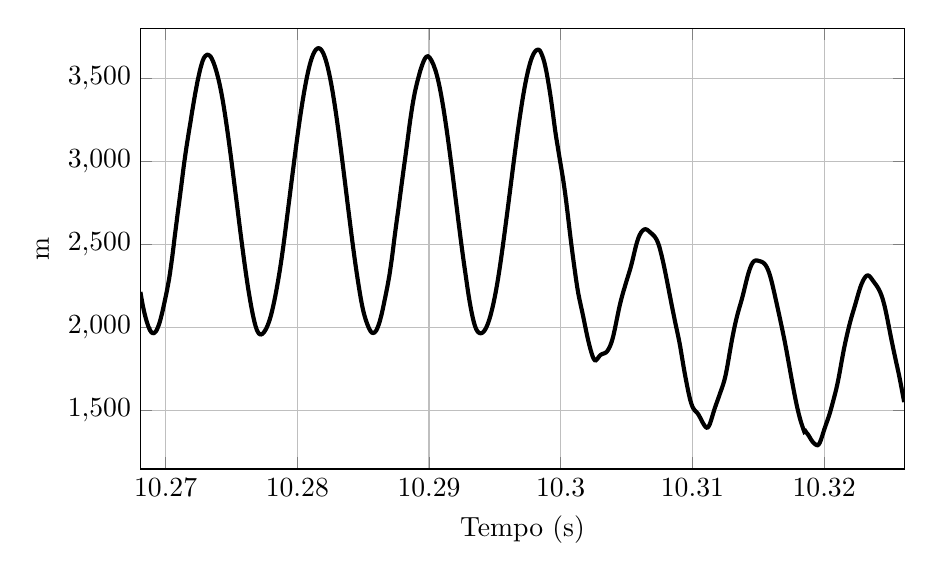
\begin{tikzpicture}

\begin{axis}[%
width=0.8\textwidth,
height=0.461611624834875\textwidth,
scale only axis,
xmin=10.2681,
xmax=10.3261,
xtick={10.27, 10.28, 10.29,  10.3, 10.31, 10.32},
xlabel={Tempo (s)},
xmajorgrids,
ymin=1150,
ymax=3800,
ytick={1500, 2000, 2500, 3000, 3500},
ylabel={m},
ymajorgrids,
scaled x ticks = false,
legend columns=-1,
legend style={/tikz/every even column/.append style={column sep=0.3cm}},
legend style={font=\footnotesize}
]
\addplot [color=black,solid,line width=1.5pt,forget plot]
  table[row sep=crcr]{10.2680833456702	2214.27689329771\\
10.2681666556704	2175.21844386467\\
10.2682499956706	2139.27194884656\\
10.2683333356708	2106.98696422299\\
10.268416675671	2078.71087725423\\
10.2684999856713	2053.53814230619\\
10.2685833256715	2031.25086664078\\
10.2686666656717	2011.53837449278\\
10.2687500056719	1994.54863011226\\
10.2688333456721	1981.24435605551\\
10.2689166556723	1971.92946687659\\
10.2689999956725	1967.18650799332\\
10.2690833356727	1966.53546960671\\
10.2691666756729	1969.83656996285\\
10.2692499856731	1976.38030097836\\
10.2693333256733	1987.29405605514\\
10.2694166656735	2002.7528793728\\
10.2695000056738	2020.50116534849\\
10.269583345674	2041.83042281776\\
10.2696666556742	2067.2919112683\\
10.2697499956744	2093.34804322286\\
10.2698333356746	2123.07174544312\\
10.2699166756748	2154.06683180132\\
10.269999985675	2184.78169762703\\
10.2700833256752	2216.32562379366\\
10.2701666656754	2251.36523756263\\
10.2702500056756	2286.8156235326\\
10.2703333456758	2328.8034264892\\
10.270416655676	2376.62732327868\\
10.2704999956763	2423.78624399154\\
10.2705833356765	2476.42708209069\\
10.2706666756767	2532.51701532693\\
10.2707499856769	2584.80711126034\\
10.2708333256771	2636.00246300238\\
10.2709166656773	2689.03433651743\\
10.2710000056775	2737.0226644036\\
10.2710833456777	2788.10236820322\\
10.2711666556779	2839.58259479396\\
10.2712499956781	2891.9359876393\\
10.2713333356783	2945.26314009518\\
10.2714166756785	2995.18785802756\\
10.2714999856788	3041.57821634999\\
10.271583325679	3087.44112992608\\
10.2716666656792	3128.3106327064\\
10.2717500056794	3170.82368263794\\
10.2718333456796	3210.37649778558\\
10.2719166556798	3250.91928652849\\
10.27199999568	3293.84312978082\\
10.2720833356802	3332.30157051341\\
10.2721666756804	3371.38155760856\\
10.2722499856806	3409.84579838596\\
10.2723333256808	3443.93355384664\\
10.272416665681	3480.03513490527\\
10.2725000056813	3509.67454083988\\
10.2725833456815	3539.96827175475\\
10.2726666556817	3566.00458357258\\
10.2727499956819	3588.86796693139\\
10.2728333356821	3608.79885337141\\
10.2729166756823	3622.71333166663\\
10.2729999856825	3631.63983590061\\
10.2730833256827	3637.62706493519\\
10.2731666656829	3640.75389710643\\
10.2732500056831	3639.57982855613\\
10.2733333456833	3635.24486664057\\
10.2734166556835	3628.94145093221\\
10.2734999956838	3617.52988056957\\
10.273583335684	3603.79506108976\\
10.2736666756842	3586.82399427944\\
10.2737499856844	3567.60682946733\\
10.2738333256846	3546.25819365635\\
10.2739166656848	3522.22374161428\\
10.274000005685	3496.99134263834\\
10.2740833456852	3468.39826476908\\
10.2741666556854	3437.54749107353\\
10.2742499956856	3403.43798215116\\
10.2743333356858	3366.834777053\\
10.274416675686	3327.15984259596\\
10.2744999856863	3285.29619694914\\
10.2745833256865	3241.26465287456\\
10.2746666656867	3195.43691586725\\
10.2747500056869	3148.12395135419\\
10.2748333456871	3099.5636799528\\
10.2749166556873	3049.92220430902\\
10.2749999956875	2999.30029648386\\
10.2750833356877	2947.95033812919\\
10.2751666756879	2895.99436931222\\
10.2752499856881	2843.67172486824\\
10.2753333256883	2790.99697448252\\
10.2754166656885	2738.20288389269\\
10.2755000056888	2685.41035615158\\
10.275583345689	2632.86818346321\\
10.2756666556892	2580.77084935005\\
10.2757499956894	2528.99041653034\\
10.2758333356896	2478.38381471251\\
10.2759166756898	2428.79214018909\\
10.27599998569	2380.29879790939\\
10.2760833256902	2333.04782367212\\
10.2761666656904	2287.40433062944\\
10.2762500056906	2243.83666984431\\
10.2763333456908	2202.55056913395\\
10.276416655691	2163.53059441337\\
10.2764999956913	2126.69676804308\\
10.2765833356915	2092.3021994563\\
10.2766666756917	2060.58172537868\\
10.2767499856919	2032.07454146687\\
10.2768333256921	2007.63877630282\\
10.2769166656923	1987.99516934387\\
10.2770000056925	1973.44457461364\\
10.2770833456927	1963.95941658216\\
10.2771666556929	1959.34146928688\\
10.2772499956931	1958.86513409068\\
10.2773333356933	1961.74815384828\\
10.2774166756935	1967.72268694806\\
10.2774999856937	1975.78804940283\\
10.277583325694	1986.44014930076\\
10.2776666656942	1999.27051076599\\
10.2777500056944	2014.22357732721\\
10.2778333456946	2031.65271184317\\
10.2779166556948	2051.64381789384\\
10.277999995695	2074.29773044596\\
10.2780833356952	2100.22014973559\\
10.2781666756954	2128.70577187549\\
10.2782499856956	2159.78171963192\\
10.2783333256958	2192.88871925628\\
10.278416665696	2227.79544823936\\
10.2785000056963	2264.59300480766\\
10.2785833456965	2302.815383778\\
10.2786666556967	2343.41362200148\\
10.2787499956969	2386.06573490754\\
10.2788333356971	2431.05288167289\\
10.2789166756973	2478.19629198396\\
10.2789999856975	2527.41466656094\\
10.2790833256977	2578.36681189604\\
10.2791666656979	2630.33344815939\\
10.2792500056981	2682.68704049477\\
10.2793333456983	2735.42552671949\\
10.2794166556985	2787.8805920193\\
10.2794999956988	2840.22505925577\\
10.279583335699	2892.24403503187\\
10.2796666756992	2943.93024698659\\
10.2797499856994	2995.41658234115\\
10.2798333256996	3046.36387678791\\
10.2799166656998	3096.63108782224\\
10.2800000057	3145.89268950001\\
10.2800833457002	3194.13870793296\\
10.2801666557004	3240.62315666616\\
10.2802499957006	3285.56010668206\\
10.2803333357008	3328.65171025375\\
10.280416675701	3370.03935003663\\
10.2804999857012	3409.33719011425\\
10.2805833257015	3446.61249342953\\
10.2806666657017	3481.78661129179\\
10.2807500057019	3514.25620213891\\
10.2808333457021	3544.36428698615\\
10.2809166557023	3571.70542609732\\
10.2809999957025	3596.03532338004\\
10.2810833357027	3617.47930525764\\
10.2811666757029	3635.57626940543\\
10.2812499857031	3650.64957165011\\
10.2813333257033	3662.70386140606\\
10.2814166657035	3671.41637266781\\
10.2815000057038	3677.18825138514\\
10.281583345704	3679.76991369225\\
10.2816666557042	3679.06849317139\\
10.2817499957044	3675.25942469529\\
10.2818333357046	3668.07833241387\\
10.2819166757048	3657.53412867541\\
10.281999985705	3643.7460429758\\
10.2820833257052	3626.51442758563\\
10.2821666657054	3606.34828817205\\
10.2822500057056	3583.04757085158\\
10.2823333457058	3556.82479352977\\
10.282416655706	3527.71597673361\\
10.2824999957063	3495.69360756855\\
10.2825833357065	3460.90979458925\\
10.2826666757067	3423.55367899944\\
10.2827499857069	3383.73106026762\\
10.2828333257071	3341.75659492356\\
10.2829166657073	3297.78626349161\\
10.2830000057075	3251.99580011992\\
10.2830833457077	3204.60400532552\\
10.2831666557079	3155.7566758269\\
10.2832499957081	3105.64473362481\\
10.2833333357083	3054.44107995157\\
10.2834166757085	3002.31741194025\\
10.2834999857087	2949.44969755693\\
10.283583325709	2896.01148063465\\
10.2836666657092	2842.26373751967\\
10.2837500057094	2788.37192170454\\
10.2838333457096	2734.60813152288\\
10.2839166557098	2681.25344664327\\
10.28399999571	2628.3185103256\\
10.2840833357102	2576.14380576492\\
10.2841666757104	2524.78342486196\\
10.2842499857106	2474.57551265656\\
10.2843333257108	2425.68835525867\\
10.284416665711	2378.68863471254\\
10.2845000057113	2333.31528305799\\
10.2845833457115	2289.47983711605\\
10.2846666557117	2247.14179242205\\
10.2847499957119	2206.49944385976\\
10.2848333357121	2168.30785941977\\
10.2849166757123	2133.47939881394\\
10.2849999857125	2102.8112591619\\
10.2850833257127	2076.86617870376\\
10.2851666657129	2054.20333179553\\
10.2852500057131	2034.11638012582\\
10.2853333457133	2016.19646585753\\
10.2854166557135	1999.89935989521\\
10.2854999957137	1986.39255909194\\
10.285583335714	1975.93400686532\\
10.2856666757142	1969.38338353815\\
10.2857499857144	1967.54245567882\\
10.2858333257146	1969.41721281149\\
10.2859166657148	1974.82362356776\\
10.286000005715	1984.07048151199\\
10.2860833457152	1997.73740928089\\
10.2861666557154	2014.83345719219\\
10.2862499957156	2034.84043808991\\
10.2863333357158	2059.3999377526\\
10.286416675716	2085.47422406052\\
10.2864999857162	2115.31887821918\\
10.2865833257165	2147.43793503352\\
10.2866666657167	2179.37772355581\\
10.2867500057169	2211.5154550808\\
10.2868333457171	2244.61816220158\\
10.2869166557173	2281.03199050223\\
10.2869999957175	2318.53634093461\\
10.2870833357177	2363.64216521267\\
10.2871666757179	2408.88012425198\\
10.2872499857181	2459.20001516784\\
10.2873333257183	2513.37399187539\\
10.2874166657185	2564.44393276787\\
10.2875000057188	2614.13990967864\\
10.287583345719	2662.55284947115\\
10.2876666557192	2708.43521433029\\
10.2877499957194	2759.31453055872\\
10.2878333357196	2809.83583516975\\
10.2879166757198	2860.0313762209\\
10.28799998572	2909.0157430463\\
10.2880833257202	2959.2985795714\\
10.2881666657204	3005.75388406762\\
10.2882500057206	3055.16757759383\\
10.2883333457208	3103.90808294046\\
10.288416655721	3154.53234410037\\
10.2884999957212	3205.89730493174\\
10.2885833357215	3253.37083302421\\
10.2886666757217	3297.71813038495\\
10.2887499857219	3340.09977115651\\
10.2888333257221	3377.44066017362\\
10.2889166657223	3412.08180830791\\
10.2890000057225	3441.70830322197\\
10.2890833457227	3469.92998183448\\
10.2891666557229	3495.10954799915\\
10.2892499957231	3519.67215120559\\
10.2893333357233	3544.19075860028\\
10.2894166757235	3564.46070229765\\
10.2894999857238	3583.31768296896\\
10.289583325724	3600.1846678847\\
10.2896666657242	3614.5263094003\\
10.2897500057244	3624.5104898149\\
10.2898333457246	3629.72439066571\\
10.2899166557248	3631.34027982252\\
10.289999995725	3626.6982844143\\
10.2900833357252	3619.44854920183\\
10.2901666757254	3608.49712316408\\
10.2902499857256	3595.27186309633\\
10.2903333257258	3580.90149273339\\
10.290416665726	3562.89367849522\\
10.2905000057262	3543.83996093639\\
10.2905833457265	3520.73633081798\\
10.2906666557267	3495.45882519165\\
10.2907499957269	3466.29201550002\\
10.2908333357271	3434.92594804349\\
10.2909166757273	3400.01419196089\\
10.2909999857275	3362.81239961591\\
10.2910833257277	3323.36817822053\\
10.2911666657279	3281.47939275236\\
10.2912500057281	3237.9937498149\\
10.2913333457283	3192.59151899513\\
10.2914166557285	3145.61535141088\\
10.2914999957287	3097.25751418909\\
10.291583335729	3047.66852094198\\
10.2916666757292	2997.08954376924\\
10.2917499857294	2945.5572971113\\
10.2918333257296	2893.36484926653\\
10.2919166657298	2840.69620902415\\
10.29200000573	2787.75297783235\\
10.2920833457302	2734.57250846685\\
10.2921666557304	2681.55510795067\\
10.2922499957306	2628.30103361967\\
10.2923333357308	2576.09768734446\\
10.292416675731	2524.85453230698\\
10.2924999857313	2474.88922826703\\
10.2925833257315	2425.95780246562\\
10.2926666657317	2378.07969690125\\
10.2927500057319	2332.56955288232\\
10.2928333457321	2286.47652551442\\
10.2929166557323	2240.71909113174\\
10.2929999957325	2196.66423226273\\
10.2930833357327	2156.47820120442\\
10.2931666757329	2119.3036575182\\
10.2932499857331	2085.51120983319\\
10.2933333257333	2055.04866724221\\
10.2934166657335	2028.71072119709\\
10.2935000057337	2007.10185793261\\
10.293583345734	1990.65196955637\\
10.2936666557342	1978.79158772434\\
10.2937499957344	1971.27876032856\\
10.2938333357346	1967.06471922034\\
10.2939166757348	1965.75835070136\\
10.293999985735	1967.06136210055\\
10.2940833257352	1970.71337001435\\
10.2941666657354	1977.33154123831\\
10.2942500057356	1986.55217618694\\
10.2943333457358	1998.38286659702\\
10.294416655736	2013.09175496916\\
10.2944999957363	2030.23217838841\\
10.2945833357365	2050.19964637644\\
10.2946666757367	2072.63197873346\\
10.2947499857369	2097.6129553117\\
10.2948333257371	2125.03786684485\\
10.2949166657373	2154.81549575199\\
10.2950000057375	2186.8636885859\\
10.2950833457377	2221.49071102371\\
10.2951666557379	2258.54122561249\\
10.2952499957381	2298.42771658018\\
10.2953333357383	2340.24061310493\\
10.2954166757385	2384.75716105106\\
10.2954999857388	2430.86253959078\\
10.295583325739	2478.43792322519\\
10.2956666657392	2527.39956642603\\
10.2957500057394	2576.93603997555\\
10.2958333457396	2627.28130228897\\
10.2959166557398	2678.16437753778\\
10.29599999574	2728.64403476382\\
10.2960833357402	2780.31386451219\\
10.2961666757404	2831.98829773568\\
10.2962499857406	2884.09949860504\\
10.2963333257408	2936.10540985912\\
10.296416665741	2987.60500621885\\
10.2965000057412	3038.49737866729\\
10.2965833457415	3088.68995969655\\
10.2966666557417	3137.78039010566\\
10.2967499957419	3185.69258906555\\
10.2968333357421	3232.44067814875\\
10.2969166757423	3277.4336951257\\
10.2969999857425	3320.96190068624\\
10.2970833257427	3362.73653999977\\
10.2971666657429	3402.44286992953\\
10.2972500057431	3440.21372972866\\
10.2973333457433	3475.38719690464\\
10.2974166557435	3507.91788250625\\
10.2974999957438	3537.70607927634\\
10.297583335744	3564.56173090337\\
10.2976666757442	3588.69719943163\\
10.2977499857444	3609.83796523401\\
10.2978333257446	3627.62131669064\\
10.2979166657448	3642.50590384204\\
10.298000005745	3654.15725135329\\
10.2980833457452	3662.79524020511\\
10.2981666557454	3668.46278564726\\
10.2982499957456	3670.95816196808\\
10.2983333357458	3670.24834584296\\
10.298416675746	3665.40306103814\\
10.2984999857463	3653.35997370642\\
10.2985833257465	3637.6584017719\\
10.2986666657467	3619.44626330933\\
10.2987500057469	3597.10405870536\\
10.2988333457471	3569.55923795729\\
10.2989166557473	3537.4104156359\\
10.2989999957475	3501.718780292\\
10.2990833357477	3462.87782910682\\
10.2991666757479	3421.67883949266\\
10.2992499857481	3378.49419524229\\
10.2993333257483	3332.24434666903\\
10.2994166657485	3282.494447177\\
10.2995000057488	3231.12908381166\\
10.299583345749	3182.37927908321\\
10.2996666557492	3138.57673540519\\
10.2997499957494	3098.33918422642\\
10.2998333357496	3058.37239388405\\
10.2999166757498	3017.87725819939\\
10.29999998575	2978.03897922223\\
10.3000833257502	2939.00469717236\\
10.3001666657504	2899.06842866613\\
10.3002500057506	2855.81668313383\\
10.3003333457508	2808.94519736475\\
10.300416655751	2757.78020294166\\
10.3004999957513	2703.56910027137\\
10.3005833357515	2647.77086606484\\
10.3006666757517	2591.76839814444\\
10.3007499857519	2536.67648729471\\
10.3008333257521	2483.56243401856\\
10.3009166657523	2432.77338529559\\
10.3010000057525	2383.62263282479\\
10.3010833457527	2335.63719380406\\
10.3011666557529	2288.77000313693\\
10.3012499957531	2244.7606796486\\
10.3013333357533	2205.99623954343\\
10.3014166757535	2172.48438878579\\
10.3014999857538	2142.17444344696\\
10.301583325754	2112.35894537785\\
10.3016666657542	2081.99749887601\\
10.3017500057544	2050.19966444207\\
10.3018333457546	2017.51424278108\\
10.3019166557548	1984.91612380422\\
10.301999995755	1953.50932853352\\
10.3020833357552	1924.12027513315\\
10.3021666757554	1896.91651332399\\
10.3022499857556	1871.73418276369\\
10.3023333257558	1848.76361822397\\
10.302416665756	1828.67745632933\\
10.3025000057563	1812.91291095333\\
10.3025833457565	1803.91313356868\\
10.3026666557567	1803.08149376202\\
10.3027499957569	1808.8832526097\\
10.3028333357571	1817.44147923199\\
10.3029166757573	1826.47755149005\\
10.3029999857575	1833.53371410071\\
10.3030833257577	1838.66285252132\\
10.3031666657579	1841.70676119141\\
10.3032500057581	1843.77583293852\\
10.3033333457583	1845.82039075475\\
10.3034166557585	1849.48022462023\\
10.3034999957588	1855.37222525086\\
10.303583335759	1864.05909842575\\
10.3036666757592	1875.40066560284\\
10.3037499857594	1889.46744663005\\
10.3038333257596	1906.44396141466\\
10.3039166657598	1926.82120447022\\
10.30400000576	1952.10961887885\\
10.3040833457602	1981.44564201052\\
10.3041666557604	2012.89850730947\\
10.3042499957606	2045.91744830588\\
10.3043333357608	2078.45649740904\\
10.304416675761	2110.34093054135\\
10.3044999857613	2139.3206173918\\
10.3045833257615	2166.64724731069\\
10.3046666657617	2190.79715937848\\
10.3047500057619	2214.69885978842\\
10.3048333457621	2236.55593638945\\
10.3049166557623	2259.08703916153\\
10.3049999957625	2280.87929803898\\
10.3050833357627	2302.14596406927\\
10.3051666757629	2323.39309996413\\
10.3052499857631	2344.78301209257\\
10.3053333257633	2368.19276825837\\
10.3054166657635	2393.60935830513\\
10.3055000057638	2420.80035076564\\
10.305583345764	2448.89393518138\\
10.3056666557642	2476.761751916\\
10.3057499957644	2501.87619171379\\
10.3058333357646	2523.77773473521\\
10.3059166757648	2543.53891036203\\
10.305999985765	2557.56880328927\\
10.3060833257652	2569.89251336344\\
10.3061666657654	2578.59014082894\\
10.3062500057656	2585.48417324507\\
10.3063333457658	2589.64100366086\\
10.306416655766	2591.57426014917\\
10.3064999957663	2590.30755340445\\
10.3065833357665	2586.97317222672\\
10.3066666757667	2581.74404479862\\
10.3067499857669	2575.87186001397\\
10.3068333257671	2570.01287164592\\
10.3069166657673	2564.30065633404\\
10.3070000057675	2558.33156387868\\
10.3070833457677	2551.63757849641\\
10.3071666557679	2543.31533809078\\
10.3072499957681	2532.60892451363\\
10.3073333357683	2519.73091257721\\
10.3074166757685	2503.22947124796\\
10.3074999857688	2483.35027624505\\
10.307583325769	2457.84273023907\\
10.3076666657692	2432.07727820207\\
10.3077500057694	2403.20555987138\\
10.3078333457696	2373.071957286\\
10.3079166557698	2341.57439870944\\
10.30799999577	2308.84963202127\\
10.3080833357702	2275.62043230656\\
10.3081666757704	2241.90416200712\\
10.3082499857706	2207.78492067777\\
10.3083333257708	2174.25165892088\\
10.308416665771	2140.0682786784\\
10.3085000057713	2107.19136439559\\
10.3085833457715	2074.74147604718\\
10.3086666557717	2042.01419993931\\
10.3087499957719	2010.57023593308\\
10.3088333357721	1980.14630384957\\
10.3089166757723	1949.42853833631\\
10.3089999857725	1917.48763375453\\
10.3090833257727	1881.58664767522\\
10.3091666657729	1842.47277018181\\
10.3092500057731	1802.13918413629\\
10.3093333457733	1762.90846842053\\
10.3094166557735	1725.65539843792\\
10.3094999957738	1690.25627821093\\
10.309583335774	1656.17909508943\\
10.3096666757742	1623.2942339076\\
10.3097499857744	1592.47270184339\\
10.3098333257746	1565.38007845786\\
10.3099166657748	1542.85830627193\\
10.310000005775	1525.3737992484\\
10.3100833457752	1512.64430252574\\
10.3101666557754	1503.39357178242\\
10.3102499957756	1496.50154694439\\
10.3103333357758	1490.01107908408\\
10.310416675776	1482.01006781764\\
10.3104999857763	1471.61484635635\\
10.3105833257765	1459.12240833022\\
10.3106666657767	1445.92153041324\\
10.3107500057769	1433.19107698867\\
10.3108333457771	1421.61735931983\\
10.3109166557773	1411.20719822021\\
10.3109999957775	1402.79685854723\\
10.3110833357777	1398.2304205806\\
10.3111666757779	1399.57645002532\\
10.3112499857781	1407.77600188853\\
10.3113333257783	1422.42843474887\\
10.3114166657785	1441.86997676702\\
10.3115000057788	1463.71661279462\\
10.311583345779	1485.83974472924\\
10.3116666557792	1506.96510272275\\
10.3117499957794	1526.67481575352\\
10.3118333357796	1545.44187697026\\
10.3119166757798	1563.87691771511\\
10.31199998578	1582.45144384593\\
10.3120833257802	1601.28052094019\\
10.3121666657804	1619.86001651548\\
10.3122500057806	1638.44412720223\\
10.3123333457808	1657.8958600391\\
10.312416655781	1679.99649325626\\
10.3124999957813	1706.40515262524\\
10.3125833357815	1737.80846868043\\
10.3126666757817	1773.4839067161\\
10.3127499857819	1811.68814541164\\
10.3128333257821	1850.64069143727\\
10.3129166657823	1888.70736083319\\
10.3130000057825	1924.98604702152\\
10.3130833457827	1959.27165358043\\
10.3131666557829	1991.89364258203\\
10.3132499957831	2022.3658358754\\
10.3133333357833	2050.86976489185\\
10.3134166757835	2077.25681158384\\
10.3134999857838	2101.40936577929\\
10.313583325784	2124.19747169132\\
10.3136666657842	2146.55186048256\\
10.3137500057844	2169.80305896171\\
10.3138333457846	2194.72383209279\\
10.3139166557848	2221.28332966895\\
10.313999995785	2248.78554294042\\
10.3140833357852	2276.09968707074\\
10.3141666757854	2302.10730133626\\
10.3142499857856	2325.944744104\\
10.3143333257858	2346.96913425782\\
10.314416665786	2364.8358930491\\
10.3145000057863	2379.7983642012\\
10.3145833457865	2390.97671647872\\
10.3146666557867	2398.48136174898\\
10.3147499957869	2402.52984279245\\
10.3148333357871	2403.85586401806\\
10.3149166757873	2403.27264996361\\
10.3149999857875	2401.81898272753\\
10.3150833257877	2400.00347743964\\
10.3151666657879	2398.08079868634\\
10.3152500057881	2395.68971927953\\
10.3153333457883	2392.40620968273\\
10.3154166557885	2387.65969785459\\
10.3154999957888	2381.05083676437\\
10.315583335789	2372.15350018032\\
10.3156666757892	2360.34174438395\\
10.3157499857894	2345.51492808496\\
10.3158333257896	2327.48836942278\\
10.3159166657898	2306.20978591483\\
10.31600000579	2281.90746766988\\
10.3160833457902	2255.16832589908\\
10.3161666557904	2226.74171529764\\
10.3162499957906	2197.41439793903\\
10.3163333357908	2167.82848812069\\
10.316416675791	2138.09339025061\\
10.3164999857913	2108.2365255589\\
10.3165833257915	2078.05474500741\\
10.3166666657917	2047.44983685667\\
10.3167500057919	2016.55986345666\\
10.3168333457921	1985.28055501932\\
10.3169166557923	1953.41554736679\\
10.3169999957925	1920.71347831611\\
10.3170833357927	1886.69901093039\\
10.3171666757929	1851.50381082758\\
10.3172499857931	1815.39573449631\\
10.3173333257933	1778.78274532416\\
10.3174166657935	1742.14676090468\\
10.3175000057938	1705.66660845987\\
10.317583345794	1669.6471539713\\
10.3176666557942	1634.3375703011\\
10.3177499957944	1599.92842425217\\
10.3178333357946	1566.73738580063\\
10.3179166757948	1535.27291811802\\
10.317999985795	1505.88603214388\\
10.3180833257952	1478.45571502022\\
10.3181666657954	1453.35014733139\\
10.3182500057956	1430.6344113615\\
10.3183333457958	1410.4233064671\\
10.318416655796	1390.89266087484\\
10.3184999957963	1373.24159293359\\
10.3185833357965	1377.65474317388\\
10.3186666757967	1367.99561170884\\
10.3187499857969	1359.8935183525\\
10.3188333257971	1350.20630531936\\
10.3189166657973	1339.06563113526\\
10.3190000057975	1328.00902722909\\
10.3190833457977	1318.10587665819\\
10.3191666557979	1309.83762094348\\
10.3192499957981	1303.47233439542\\
10.3193333357983	1298.11707798471\\
10.3194166757985	1293.85544936265\\
10.3194999857988	1292.44741244711\\
10.319583325799	1296.69875580802\\
10.3196666657992	1307.09103609654\\
10.3197500057994	1322.90021049034\\
10.3198333457996	1342.48755446406\\
10.3199166557998	1363.38417715463\\
10.3199999958	1384.25092275626\\
10.3200833358002	1403.93746970142\\
10.3201666758004	1422.83702453126\\
10.3202499858006	1441.20316733492\\
10.3203333258008	1460.22541996907\\
10.320416665801	1480.57344907256\\
10.3205000058013	1502.96681194577\\
10.3205833458015	1527.09311337106\\
10.3206666558017	1551.54158796007\\
10.3207499958019	1576.7879129287\\
10.3208333358021	1601.9216271331\\
10.3209166758023	1628.3595043389\\
10.3209999858025	1657.20721936924\\
10.3210833258027	1688.94182572141\\
10.3211666658029	1723.80187459507\\
10.3212500058031	1760.41314626978\\
10.3213333458033	1797.86483923587\\
10.3214166558035	1833.5554510085\\
10.3214999958038	1868.59299315302\\
10.321583335804	1900.1955325161\\
10.3216666758042	1931.02953768495\\
10.3217499858044	1959.77569432088\\
10.3218333258046	1987.96771786097\\
10.3219166658048	2014.63148408345\\
10.322000005805	2039.93673540556\\
10.3220833458052	2064.16739435613\\
10.3221666558054	2086.22509169101\\
10.3222499958056	2108.05562014678\\
10.3223333358058	2130.18393368314\\
10.322416675806	2152.8242647105\\
10.3224999858063	2176.08800329617\\
10.3225833258065	2199.65888566206\\
10.3226666658067	2221.57237405839\\
10.3227500058069	2242.46856172116\\
10.3228333458071	2260.1510063343\\
10.3229166558073	2275.08269738925\\
10.3229999958075	2288.49018109067\\
10.3230833358077	2299.17056740676\\
10.3231666758079	2307.82801411172\\
10.3232499858081	2312.74351945049\\
10.3233333258083	2313.66061065477\\
10.3234166658085	2310.59273591489\\
10.3235000058088	2304.45512088456\\
10.323583345809	2296.06900934042\\
10.3236666558092	2286.78118752612\\
10.3237499958094	2277.60018225267\\
10.3238333358096	2268.71052965767\\
10.3239166758098	2259.71253979401\\
10.32399998581	2250.45749550797\\
10.3240833258102	2239.95415123491\\
10.3241666658104	2228.13570038633\\
10.3242500058106	2214.58200095957\\
10.3243333458108	2198.42482319276\\
10.324416655811	2180.05506875758\\
10.3244999958113	2157.79111283327\\
10.3245833358115	2132.70956341809\\
10.3246666758117	2104.22146356531\\
10.3247499858119	2073.14698656407\\
10.3248333258121	2040.10072455341\\
10.3249166658123	2006.21673136933\\
10.3250000058125	1972.41596742013\\
10.3250833458127	1939.19238325087\\
10.3251666558129	1906.57063856619\\
10.3252499958131	1874.542364097\\
10.3253333358133	1843.29483782318\\
10.3254166758135	1812.74541757922\\
10.3254999858138	1782.74987695046\\
10.325583325814	1753.22803501223\\
10.3256666658142	1722.52497764069\\
10.3257500058144	1690.25983138032\\
10.3258333458146	1656.29798030712\\
10.3259166558148	1621.37969232152\\
10.325999995815	1586.34981434271\\
10.3260833358152	1552.04237987092\\
};
\end{axis}
\end{tikzpicture}%}}
    \end{figure}
    \end{small}
    \vfill
  }

  \frame{
    \frametitle{\insertsection}
    \vfill
    \begin{small}
    \begin{figure}[htb]
      \centering
      \raisebox{-0.5\height}{
        %\def\svgwidth{0.8\linewidth}
        \resizebox{0.9\linewidth}{!}{% This file was created by matlab2tikz v0.4.7 running on MATLAB 7.14.
% Copyright (c) 2008--2014, Nico Schlömer <nico.schloemer@gmail.com>
% All rights reserved.
% Minimal pgfplots version: 1.3
% 
% The latest updates can be retrieved from
%   http://www.mathworks.com/matlabcentral/fileexchange/22022-matlab2tikz
% where you can also make suggestions and rate matlab2tikz.
% 
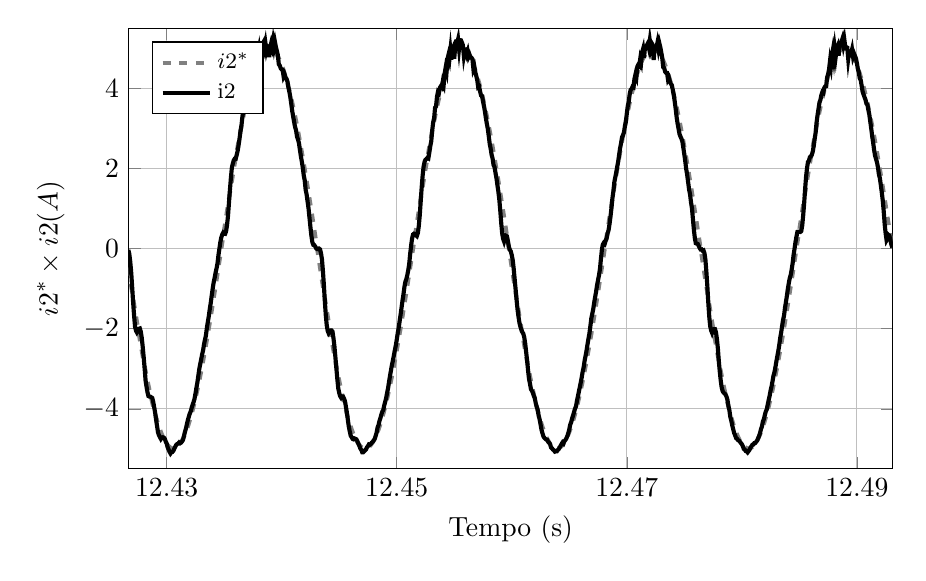
\begin{tikzpicture}

\begin{axis}[%
width=0.8\textwidth,
height=0.461611624834875\textwidth,
scale only axis,
xmin=12.4267,
xmax=12.4931,
xtick={12.43, 12.45, 12.47, 12.49},
xlabel={Tempo (s)},
xmajorgrids,
ymin=-5.5,
ymax=5.5,
ytick={-4, -2,  0,  2,  4},
ylabel={$\text{i2}^\text{*}\text{ }\times\text{ i2 (A)}$},
ymajorgrids,
legend style={at={(0.03,0.97)},anchor=north west,draw=black,fill=white,legend cell align=left},
scaled x ticks = false,
legend style={font=\footnotesize}
]
\addplot [color=gray,dashed,line width=1.5pt]
  table[row sep=crcr]{12.4266666610667	-0.469922358851241\\
12.4267500010669	-0.625738349089735\\
12.4268333410671	-0.780936811123984\\
12.4269166510673	-0.935364582809298\\
12.4269999910675	-1.08886926257931\\
12.4270833310677	-1.24129935984794\\
12.4271666710679	-1.39250444451229\\
12.4272500110681	-1.542335295409\\
12.4273333210683	-1.69064404757754\\
12.4274166610685	-1.83728433818505\\
12.4275000010688	-1.9821114509688\\
12.427583341069	-2.12498245905366\\
12.4276666510692	-2.26575636600367\\
12.4277499910694	-2.40429424496852\\
12.4278333310696	-2.54045937578755\\
12.4279166710698	-2.67411737991605\\
12.42800001107	-2.80513635304068\\
12.4280833210702	-2.93338699525307\\
12.4281666610704	-3.05874273865325\\
12.4282500010706	-3.18107987225687\\
12.4283333410708	-3.300277664083\\
12.428416651071	-3.41621848030203\\
12.4284999910713	-3.52878790132605\\
12.4285833310715	-3.6378748347272\\
12.4286666710717	-3.74337162487242\\
12.4287500110719	-3.84517415916662\\
12.4288333210721	-3.94318197079923\\
12.4289166610723	-4.03729833789279\\
12.4290000010725	-4.12743037895578\\
12.4290833410727	-4.21348914454545\\
12.4291666510729	-4.29538970505017\\
12.4292499910731	-4.37305123450468\\
12.4293333310733	-4.44639709035561\\
12.4294166710735	-4.51535488909839\\
12.4295000110738	-4.57985657771103\\
12.429583321074	-4.63983850081426\\
12.4296666610742	-4.69524146349167\\
12.4297500010744	-4.74601078970799\\
12.4298333410746	-4.79209637626769\\
12.4299166510748	-4.83345274226082\\
12.429999991075	-4.87003907394716\\
12.4300833310752	-4.90181926503446\\
12.4301666710754	-4.92876195231098\\
12.4302500110756	-4.95084054659722\\
12.4303333210758	-4.96803325898618\\
12.430416661076	-4.98032312234645\\
12.4305000010763	-4.98769800806666\\
12.4305833410765	-4.99015063802499\\
12.4306666510767	-4.98767859177177\\
12.4307499910769	-4.98028430891821\\
12.4308333310771	-4.96797508672876\\
12.4309166710773	-4.95076307291961\\
12.4310000110775	-4.92866525367035\\
12.4310833210777	-4.90170343686069\\
12.4311666610779	-4.86990423054868\\
12.4312500010781	-4.83329901671178\\
12.4313333410783	-4.79192392027664\\
12.4314166510785	-4.74581977346818\\
12.4314999910788	-4.69503207551307\\
12.431583331079	-4.63961094773752\\
12.4316666710792	-4.57961108410357\\
12.4317500110794	-4.51509169723276\\
12.4318333210796	-4.44611645997041\\
12.4319166610798	-4.37275344254821\\
12.43200000108	-4.29507504540713\\
12.4320833410802	-4.21315792774694\\
12.4321666510804	-4.12708293187278\\
12.4322499910806	-4.03693500341362\\
12.4323333310808	-3.94280310749116\\
12.432416671081	-3.844780140922\\
12.4325000110813	-3.74296284053967\\
12.4325833210815	-3.63745168772712\\
12.4326666610817	-3.52835080925364\\
12.4327500010819	-3.41576787451438\\
12.4328333410821	-3.29981398927364\\
12.4329166510823	-3.18060358601685\\
12.4329999910825	-3.05825431101958\\
12.4330833310827	-2.93288690824486\\
12.4331666710829	-2.80462510018342\\
12.4332500110831	-2.6735954657546\\
12.4333333210833	-2.53992731538817\\
12.4334166610835	-2.40375256341059\\
12.4335000010838	-2.26520559786149\\
12.433583341084	-2.12442314786889\\
12.4336666510842	-1.98154414871406\\
12.4337499910844	-1.83670960471917\\
12.4338333310846	-1.69006245009306\\
12.4339166710848	-1.54174740787242\\
12.434000011085	-1.39191084709763\\
12.4340833210852	-1.24070063836418\\
12.4341666610854	-1.08826600789228\\
12.4342500010856	-0.934757390258532\\
12.4343333410858	-0.780326279935228\\
12.434416651086	-0.625125081783561\\
12.4344999910863	-0.469306960648439\\
12.4345833310865	-0.313025690203273\\
12.4346666710867	-0.156435501193926\\
12.4347500110869	0.000309070768412356\\
12.4348333210871	0.157053337715217\\
12.4349166610873	0.313642611978976\\
12.4350000010875	0.469922358851243\\
12.4350833410877	0.625738349089738\\
12.4351666510879	0.780936811123987\\
12.4352499910881	0.935364582809301\\
12.4353333310883	1.08886926257932\\
12.4354166710885	1.24129935984795\\
12.4355000110888	1.39250444451229\\
12.435583321089	1.54233529540901\\
12.4356666610892	1.69064404757755\\
12.4357500010894	1.83728433818506\\
12.4358333410896	1.98211145096881\\
12.4359166510898	2.12498245905367\\
12.43599999109	2.26575636600368\\
12.4360833310902	2.40429424496853\\
12.4361666710904	2.54045937578756\\
12.4362500110906	2.67411737991606\\
12.4363333210908	2.80513635304069\\
12.436416661091	2.93338699525308\\
12.4365000010913	3.05874273865327\\
12.4365833410915	3.18107987225688\\
12.4366666510917	3.30027766408301\\
12.4367499910919	3.41621848030204\\
12.4368333310921	3.52878790132607\\
12.4369166710923	3.63787483472721\\
12.4370000110925	3.74337162487243\\
12.4370833210927	3.84517415916664\\
12.4371666610929	3.94318197079924\\
12.4372500010931	4.0372983378928\\
12.4373333410933	4.1274303789558\\
12.4374166510935	4.21348914454547\\
12.4374999910938	4.29538970505019\\
12.437583331094	4.3730512345047\\
12.4376666710942	4.44639709035563\\
12.4377500110944	4.51535488909841\\
12.4378333210946	4.57985657771105\\
12.4379166610948	4.63983850081428\\
12.438000001095	4.69524146349169\\
12.4380833410952	4.746010789708\\
12.4381666510954	4.79209637626771\\
12.4382499910956	4.83345274226084\\
12.4383333310958	4.87003907394718\\
12.438416671096	4.90181926503448\\
12.4385000110963	4.928761952311\\
12.4385833210965	4.95084054659724\\
12.4386666610967	4.9680332589862\\
12.4387500010969	4.98032312234647\\
12.4388333410971	4.98769800806668\\
12.4389166510973	4.99015063802501\\
12.4389999910975	4.9876785917718\\
12.4390833310977	4.98028430891823\\
12.4391666710979	4.96797508672878\\
12.4392500110981	4.95076307291963\\
12.4393333210983	4.92866525367038\\
12.4394166610985	4.90170343686072\\
12.4395000010988	4.8699042305487\\
12.439583341099	4.8332990167118\\
12.4396666510992	4.79192392027667\\
12.4397499910994	4.7458197734682\\
12.4398333310996	4.69503207551309\\
12.4399166710998	4.63961094773754\\
12.4400000111	4.57961108410359\\
12.4400833211002	4.51509169723278\\
12.4401666611004	4.44611645997043\\
12.4402500011006	4.37275344254823\\
12.4403333411008	4.29507504540715\\
12.440416651101	4.21315792774696\\
12.4404999911013	4.1270829318728\\
12.4405833311015	4.03693500341364\\
12.4406666711017	3.94280310749118\\
12.4407500111019	3.84478014092201\\
12.4408333211021	3.74296284053969\\
12.4409166611023	3.63745168772713\\
12.4410000011025	3.52835080925365\\
12.4410833411027	3.4157678745144\\
12.4411666511029	3.29981398927365\\
12.4412499911031	3.18060358601686\\
12.4413333311033	3.05825431101959\\
12.4414166711035	2.93288690824487\\
12.4415000111038	2.80462510018344\\
12.441583321104	2.67359546575461\\
12.4416666611042	2.53992731538818\\
12.4417500011044	2.40375256341061\\
12.4418333411046	2.26520559786151\\
12.4419166511048	2.1244231478689\\
12.441999991105	1.98154414871407\\
12.4420833311052	1.83670960471918\\
12.4421666711054	1.69006245009306\\
12.4422500111056	1.54174740787242\\
12.4423333211058	1.39191084709763\\
12.442416661106	1.24070063836419\\
12.4425000011063	1.08826600789228\\
12.4425833411065	0.934757390258537\\
12.4426666511067	0.780326279935231\\
12.4427499911069	0.625125081783564\\
12.4428333311071	0.469306960648441\\
12.4429166711073	0.313025690203275\\
12.4430000111075	0.156435501193927\\
12.4430833211077	-0.000309070768411981\\
12.4431666611079	-0.157053337715217\\
12.4432500011081	-0.313642611978977\\
12.4433333411083	-0.469922358851244\\
12.4434166511085	-0.62573834908974\\
12.4434999911088	-0.78093681112399\\
12.443583331109	-0.935364582809305\\
12.4436666711092	-1.08886926257932\\
12.4437500111094	-1.24129935984795\\
12.4438333211096	-1.3925044445123\\
12.4439166611098	-1.54233529540901\\
12.44400000111	-1.69064404757755\\
12.4440833411102	-1.83728433818507\\
12.4441666511104	-1.98211145096882\\
12.4442499911106	-2.12498245905368\\
12.4443333311108	-2.26575636600369\\
12.444416671111	-2.40429424496854\\
12.4445000111113	-2.54045937578757\\
12.4445833211115	-2.67411737991607\\
12.4446666611117	-2.8051363530407\\
12.4447500011119	-2.93338699525309\\
12.4448333411121	-3.05874273865328\\
12.4449166511123	-3.1810798722569\\
12.4449999911125	-3.30027766408303\\
12.4450833311127	-3.41621848030206\\
12.4451666711129	-3.52878790132608\\
12.4452500111131	-3.63787483472723\\
12.4453333211133	-3.74337162487245\\
12.4454166611135	-3.84517415916665\\
12.4455000011138	-3.94318197079926\\
12.445583341114	-4.03729833789282\\
12.4456666511142	-4.12743037895581\\
12.4457499911144	-4.21348914454549\\
12.4458333311146	-4.2953897050502\\
12.4459166711148	-4.37305123450472\\
12.446000011115	-4.44639709035565\\
12.4460833211152	-4.51535488909843\\
12.4461666611154	-4.57985657771107\\
12.4462500011156	-4.6398385008143\\
12.4463333411158	-4.69524146349171\\
12.446416651116	-4.74601078970803\\
12.4464999911163	-4.79209637626773\\
12.4465833311165	-4.83345274226086\\
12.4466666711167	-4.8700390739472\\
12.4467500111169	-4.9018192650345\\
12.4468333211171	-4.92876195231102\\
12.4469166611173	-4.95084054659726\\
12.4470000011175	-4.96803325898622\\
12.4470833411177	-4.98032312234649\\
12.4471666511179	-4.9876980080667\\
12.4472499911181	-4.99015063802503\\
12.4473333311183	-4.98767859177181\\
12.4474166711185	-4.98028430891825\\
12.4475000111188	-4.9679750867288\\
12.447583321119	-4.95076307291965\\
12.4476666611192	-4.9286652536704\\
12.4477500011194	-4.90170343686074\\
12.4478333411196	-4.86990423054872\\
12.4479166511198	-4.83329901671182\\
12.44799999112	-4.79192392027668\\
12.4480833311202	-4.74581977346822\\
12.4481666711204	-4.69503207551311\\
12.4482500111206	-4.63961094773756\\
12.4483333211208	-4.57961108410361\\
12.448416661121	-4.5150916972328\\
12.4485000011213	-4.44611645997045\\
12.4485833411215	-4.37275344254825\\
12.4486666511217	-4.29507504540717\\
12.4487499911219	-4.21315792774698\\
12.4488333311221	-4.12708293187281\\
12.4489166711223	-4.03693500341365\\
12.4490000111225	-3.94280310749119\\
12.4490833211227	-3.84478014092203\\
12.4491666611229	-3.74296284053971\\
12.4492500011231	-3.63745168772715\\
12.4493333411233	-3.52835080925367\\
12.4494166511235	-3.41576787451441\\
12.4494999911238	-3.29981398927367\\
12.449583331124	-3.18060358601687\\
12.4496666711242	-3.05825431101961\\
12.4497500111244	-2.93288690824488\\
12.4498333211246	-2.80462510018345\\
12.4499166611248	-2.67359546575463\\
12.450000001125	-2.5399273153882\\
12.4500833411252	-2.40375256341062\\
12.4501666511254	-2.26520559786152\\
12.4502499911256	-2.12442314786891\\
12.4503333311258	-1.98154414871408\\
12.450416671126	-1.83670960471919\\
12.4505000111263	-1.69006245009307\\
12.4505833211265	-1.54174740787243\\
12.4506666611267	-1.39191084709764\\
12.4507500011269	-1.2407006383642\\
12.4508333411271	-1.08826600789229\\
12.4509166511273	-0.934757390258543\\
12.4509999911275	-0.780326279935237\\
12.4510833311277	-0.625125081783569\\
12.4511666711279	-0.469306960648446\\
12.4512500111281	-0.313025690203278\\
12.4513333211283	-0.15643550119393\\
12.4514166611285	0.000309070768409497\\
12.4515000011288	0.157053337715215\\
12.451583341129	0.313642611978976\\
12.4516666511292	0.469922358851244\\
12.4517499911294	0.62573834908974\\
12.4518333311296	0.780936811123991\\
12.4519166711298	0.935364582809307\\
12.45200001113	1.08886926257932\\
12.4520833211302	1.24129935984795\\
12.4521666611304	1.3925044445123\\
12.4522500011306	1.54233529540902\\
12.4523333411308	1.69064404757756\\
12.452416651131	1.83728433818507\\
12.4524999911313	1.98211145096882\\
12.4525833311315	2.12498245905368\\
12.4526666711317	2.2657563660037\\
12.4527500111319	2.40429424496855\\
12.4528333211321	2.54045937578758\\
12.4529166611323	2.67411737991608\\
12.4530000011325	2.80513635304071\\
12.4530833411327	2.9333869952531\\
12.4531666511329	3.05874273865329\\
12.4532499911331	3.18107987225691\\
12.4533333311333	3.30027766408304\\
12.4534166711335	3.41621848030207\\
12.4535000111338	3.5287879013261\\
12.453583321134	3.63787483472724\\
12.4536666611342	3.74337162487246\\
12.4537500011344	3.84517415916667\\
12.4538333411346	3.94318197079928\\
12.4539166511348	4.03729833789283\\
12.453999991135	4.12743037895583\\
12.4540833311352	4.2134891445455\\
12.4541666711354	4.29538970505022\\
12.4542500111356	4.37305123450473\\
12.4543333211358	4.44639709035567\\
12.454416661136	4.51535488909845\\
12.4545000011363	4.57985657771109\\
12.4545833411365	4.63983850081431\\
12.4546666511367	4.69524146349173\\
12.4547499911369	4.74601078970804\\
12.4548333311371	4.79209637626775\\
12.4549166711373	4.83345274226088\\
12.4550000111375	4.87003907394722\\
12.4550833211377	4.90181926503452\\
12.4551666611379	4.92876195231105\\
12.4552500011381	4.95084054659728\\
12.4553333411383	4.96803325898624\\
12.4554166511385	4.98032312234651\\
12.4554999911387	4.98769800806672\\
12.455583331139	4.99015063802505\\
12.4556666711392	4.98767859177184\\
12.4557500111394	4.98028430891828\\
12.4558333211396	4.96797508672882\\
12.4559166611398	4.95076307291967\\
12.45600000114	4.92866525367042\\
12.4560833411402	4.90170343686076\\
12.4561666511404	4.86990423054874\\
12.4562499911406	4.83329901671184\\
12.4563333311408	4.79192392027671\\
12.456416671141	4.74581977346824\\
12.4565000111413	4.69503207551313\\
12.4565833211415	4.63961094773758\\
12.4566666611417	4.57961108410363\\
12.4567500011419	4.51509169723282\\
12.4568333411421	4.44611645997047\\
12.4569166511423	4.37275344254827\\
12.4569999911425	4.29507504540719\\
12.4570833311427	4.21315792774699\\
12.4571666711429	4.12708293187283\\
12.4572500111431	4.03693500341367\\
12.4573333211433	3.94280310749121\\
12.4574166611435	3.84478014092205\\
12.4575000011438	3.74296284053972\\
12.457583341144	3.63745168772717\\
12.4576666511442	3.52835080925369\\
12.4577499911444	3.41576787451443\\
12.4578333311446	3.29981398927368\\
12.4579166711448	3.18060358601689\\
12.458000011145	3.05825431101962\\
12.4580833211452	2.9328869082449\\
12.4581666611454	2.80462510018346\\
12.4582500011456	2.67359546575464\\
12.4583333411458	2.53992731538821\\
12.458416651146	2.40375256341063\\
12.4584999911462	2.26520559786153\\
12.4585833311465	2.12442314786892\\
12.4586666711467	1.98154414871409\\
12.4587500111469	1.83670960471919\\
12.4588333211471	1.69006245009308\\
12.4589166611473	1.54174740787244\\
12.4590000011475	1.39191084709765\\
12.4590833411477	1.2407006383642\\
12.4591666511479	1.0882660078923\\
12.4592499911481	0.934757390258548\\
12.4593333311483	0.780326279935242\\
12.4594166711485	0.625125081783573\\
12.4595000111488	0.469306960648449\\
12.459583321149	0.313025690203281\\
12.4596666611492	0.156435501193932\\
12.4597500011494	-0.000309070768407999\\
12.4598333411496	-0.157053337715214\\
12.4599166511498	-0.313642611978975\\
12.45999999115	-0.469922358851244\\
12.4600833311502	-0.625738349089741\\
12.4601666711504	-0.780936811123993\\
12.4602500111506	-0.935364582809309\\
12.4603333211508	-1.08886926257933\\
12.460416661151	-1.24129935984796\\
12.4605000011512	-1.39250444451231\\
12.4605833411515	-1.54233529540902\\
12.4606666511517	-1.69064404757756\\
12.4607499911519	-1.83728433818508\\
12.4608333311521	-1.98211145096883\\
12.4609166711523	-2.12498245905369\\
12.4610000111525	-2.2657563660037\\
12.4610833211527	-2.40429424496856\\
12.4611666611529	-2.54045937578758\\
12.4612500011531	-2.67411737991609\\
12.4613333411533	-2.80513635304072\\
12.4614166511535	-2.93338699525312\\
12.4614999911537	-3.0587427386533\\
12.461583331154	-3.18107987225692\\
12.4616666711542	-3.30027766408305\\
12.4617500111544	-3.41621848030208\\
12.4618333211546	-3.52878790132611\\
12.4619166611548	-3.63787483472725\\
12.462000001155	-3.74337162487248\\
12.4620833411552	-3.84517415916668\\
12.4621666511554	-3.94318197079929\\
12.4622499911556	-4.03729833789285\\
12.4623333311558	-4.12743037895585\\
12.462416671156	-4.21348914454552\\
12.4625000111563	-4.29538970505024\\
12.4625833211565	-4.37305123450475\\
12.4626666611567	-4.44639709035569\\
12.4627500011569	-4.51535488909847\\
12.4628333411571	-4.57985657771111\\
12.4629166511573	-4.63983850081433\\
12.4629999911575	-4.69524146349175\\
12.4630833311577	-4.74601078970806\\
12.4631666711579	-4.79209637626777\\
12.4632500111581	-4.8334527422609\\
12.4633333211583	-4.87003907394724\\
12.4634166611585	-4.90181926503454\\
12.4635000011587	-4.92876195231107\\
12.463583341159	-4.9508405465973\\
12.4636666511592	-4.96803325898627\\
12.4637499911594	-4.98032312234654\\
12.4638333311596	-4.98769800806675\\
12.4639166711598	-4.99015063802507\\
12.46400001116	-4.98767859177186\\
12.4640833211602	-4.9802843089183\\
12.4641666611604	-4.96797508672885\\
12.4642500011606	-4.95076307291969\\
12.4643333411608	-4.92866525367044\\
12.464416651161	-4.90170343686078\\
12.4644999911613	-4.86990423054877\\
12.4645833311615	-4.83329901671186\\
12.4646666711617	-4.79192392027673\\
12.4647500111619	-4.74581977346826\\
12.4648333211621	-4.69503207551315\\
12.4649166611623	-4.6396109477376\\
12.4650000011625	-4.57961108410365\\
12.4650833411627	-4.51509169723284\\
12.4651666511629	-4.44611645997049\\
12.4652499911631	-4.37275344254829\\
12.4653333311633	-4.29507504540721\\
12.4654166711635	-4.21315792774702\\
12.4655000111638	-4.12708293187285\\
12.465583321164	-4.03693500341369\\
12.4656666611642	-3.94280310749123\\
12.4657500011644	-3.84478014092207\\
12.4658333411646	-3.74296284053974\\
12.4659166511648	-3.63745168772718\\
12.465999991165	-3.5283508092537\\
12.4660833311652	-3.41576787451445\\
12.4661666711654	-3.2998139892737\\
12.4662500111656	-3.1806035860169\\
12.4663333211658	-3.05825431101964\\
12.466416661166	-2.93288690824491\\
12.4665000011662	-2.80462510018348\\
12.4665833411665	-2.67359546575465\\
12.4666666511667	-2.53992731538822\\
12.4667499911669	-2.40375256341064\\
12.4668333311671	-2.26520559786154\\
12.4669166711673	-2.12442314786894\\
12.4670000111675	-1.9815441487141\\
12.4670833211677	-1.83670960471921\\
12.4671666611679	-1.69006245009309\\
12.4672500011681	-1.54174740787245\\
12.4673333411683	-1.39191084709766\\
12.4674166511685	-1.24070063836421\\
12.4674999911688	-1.0882660078923\\
12.467583331169	-0.934757390258555\\
12.4676666711692	-0.780326279935248\\
12.4677500111694	-0.625125081783578\\
12.4678333211696	-0.469306960648454\\
12.4679166611698	-0.313025690203285\\
12.46800000117	-0.156435501193936\\
12.4680833411702	0.000309070768405348\\
12.4681666511704	0.157053337715213\\
12.4682499911706	0.313642611978974\\
12.4683333311708	0.469922358851244\\
12.468416671171	0.625738349089741\\
12.4685000111712	0.780936811123994\\
12.4685833211715	0.935364582809311\\
12.4686666611717	1.08886926257933\\
12.4687500011719	1.24129935984796\\
12.4688333411721	1.39250444451231\\
12.4689166511723	1.54233529540903\\
12.4689999911725	1.69064404757757\\
12.4690833311727	1.83728433818509\\
12.4691666711729	1.98211145096884\\
12.4692500111731	2.1249824590537\\
12.4693333211733	2.26575636600371\\
12.4694166611735	2.40429424496857\\
12.4695000011738	2.5404593757876\\
12.469583341174	2.6741173799161\\
12.4696666511742	2.80513635304073\\
12.4697499911744	2.93338699525313\\
12.4698333311746	3.05874273865331\\
12.4699166711748	3.18107987225693\\
12.470000011175	3.30027766408306\\
12.4700833211752	3.4162184803021\\
12.4701666611754	3.52878790132612\\
12.4702500011756	3.63787483472727\\
12.4703333411758	3.74337162487249\\
12.470416651176	3.8451741591667\\
12.4704999911763	3.94318197079931\\
12.4705833311765	4.03729833789287\\
12.4706666711767	4.12743037895587\\
12.4707500111769	4.21348914454554\\
12.4708333211771	4.29538970505026\\
12.4709166611773	4.37305123450478\\
12.4710000011775	4.44639709035571\\
12.4710833411777	4.51535488909849\\
12.4711666511779	4.57985657771113\\
12.4712499911781	4.63983850081436\\
12.4713333311783	4.69524146349177\\
12.4714166711785	4.74601078970809\\
12.4715000111787	4.79209637626779\\
12.471583321179	4.83345274226092\\
12.4716666611792	4.87003907394727\\
12.4717500011794	4.90181926503457\\
12.4718333411796	4.92876195231109\\
12.4719166511798	4.95084054659732\\
12.47199999118	4.96803325898629\\
12.4720833311802	4.98032312234656\\
12.4721666711804	4.98769800806677\\
12.4722500111806	4.9901506380251\\
12.4723333211808	4.98767859177188\\
12.472416661181	4.98028430891832\\
12.4725000011813	4.96797508672887\\
12.4725833411815	4.95076307291972\\
12.4726666511817	4.92866525367046\\
12.4727499911819	4.9017034368608\\
12.4728333311821	4.86990423054879\\
12.4729166711823	4.83329901671189\\
12.4730000111825	4.79192392027675\\
12.4730833211827	4.74581977346829\\
12.4731666611829	4.69503207551318\\
12.4732500011831	4.63961094773763\\
12.4733333411833	4.57961108410368\\
12.4734166511835	4.51509169723287\\
12.4734999911838	4.44611645997051\\
12.473583331184	4.37275344254831\\
12.4736666711842	4.29507504540723\\
12.4737500111844	4.21315792774704\\
12.4738333211846	4.12708293187287\\
12.4739166611848	4.03693500341371\\
12.474000001185	3.94280310749125\\
12.4740833411852	3.84478014092209\\
12.4741666511854	3.74296284053976\\
12.4742499911856	3.6374516877272\\
12.4743333311858	3.52835080925372\\
12.474416671186	3.41576787451446\\
12.4745000111862	3.29981398927371\\
12.4745833211865	3.18060358601692\\
12.4746666611867	3.05825431101965\\
12.4747500011869	2.93288690824493\\
12.4748333411871	2.80462510018349\\
12.4749166511873	2.67359546575467\\
12.4749999911875	2.53992731538823\\
12.4750833311877	2.40375256341065\\
12.4751666711879	2.26520559786155\\
12.4752500111881	2.12442314786895\\
12.4753333211883	1.98154414871411\\
12.4754166611885	1.83670960471922\\
12.4755000011888	1.6900624500931\\
12.475583341189	1.54174740787246\\
12.4756666511892	1.39191084709767\\
12.4757499911894	1.24070063836422\\
12.4758333311896	1.08826600789231\\
12.4759166711898	0.934757390258562\\
12.47600001119	0.780326279935254\\
12.4760833211902	0.625125081783583\\
12.4761666611904	0.469306960648458\\
12.4762500011906	0.313025690203289\\
12.4763333411908	0.156435501193938\\
12.476416651191	-0.000309070768403377\\
12.4764999911913	-0.157053337715211\\
12.4765833311915	-0.313642611978974\\
12.4766666711917	-0.469922358851244\\
12.4767500111919	-0.625738349089743\\
12.4768333211921	-0.780936811123996\\
12.4769166611923	-0.935364582809313\\
12.4770000011925	-1.08886926257933\\
12.4770833411927	-1.24129935984797\\
12.4771666511929	-1.39250444451232\\
12.4772499911931	-1.54233529540903\\
12.4773333311933	-1.69064404757758\\
12.4774166711935	-1.83728433818509\\
12.4775000111938	-1.98211145096884\\
12.477583321194	-2.12498245905371\\
12.4776666611942	-2.26575636600372\\
12.4777500011944	-2.40429424496858\\
12.4778333411946	-2.54045937578761\\
12.4779166511948	-2.67411737991611\\
12.477999991195	-2.80513635304074\\
12.4780833311952	-2.93338699525314\\
12.4781666711954	-3.05874273865333\\
12.4782500111956	-3.18107987225695\\
12.4783333211958	-3.30027766408308\\
12.478416661196	-3.41621848030211\\
12.4785000011963	-3.52878790132614\\
12.4785833411965	-3.63787483472729\\
12.4786666511967	-3.74337162487251\\
12.4787499911969	-3.84517415916672\\
12.4788333311971	-3.94318197079933\\
12.4789166711973	-4.03729833789289\\
12.4790000111975	-4.12743037895588\\
12.4790833211977	-4.21348914454556\\
12.4791666611979	-4.29538970505028\\
12.4792500011981	-4.37305123450479\\
12.4793333411983	-4.44639709035573\\
12.4794166511985	-4.51535488909851\\
12.4794999911988	-4.57985657771115\\
12.479583331199	-4.63983850081438\\
12.4796666711992	-4.69524146349179\\
12.4797500111994	-4.74601078970811\\
12.4798333211996	-4.79209637626781\\
12.4799166611998	-4.83345274226095\\
12.4800000012	-4.87003907394729\\
12.4800833412002	-4.90181926503459\\
12.4801666512004	-4.92876195231112\\
12.4802499912006	-4.95084054659735\\
12.4803333312008	-4.96803325898631\\
12.480416671201	-4.98032312234658\\
12.4805000112013	-4.9876980080668\\
12.4805833212015	-4.99015063802512\\
12.4806666612017	-4.98767859177191\\
12.4807500012019	-4.98028430891835\\
12.4808333412021	-4.96797508672889\\
12.4809166512023	-4.95076307291974\\
12.4809999912025	-4.92866525367049\\
12.4810833312027	-4.90170343686083\\
12.4811666712029	-4.86990423054881\\
12.4812500112031	-4.83329901671191\\
12.4813333212033	-4.79192392027677\\
12.4814166612035	-4.74581977346831\\
12.4815000012038	-4.6950320755132\\
12.481583341204	-4.63961094773765\\
12.4816666512042	-4.5796110841037\\
12.4817499912044	-4.51509169723289\\
12.4818333312046	-4.44611645997053\\
12.4819166712048	-4.37275344254833\\
12.482000011205	-4.29507504540725\\
12.4820833212052	-4.21315792774706\\
12.4821666612054	-4.12708293187289\\
12.4822500012056	-4.03693500341373\\
12.4823333412058	-3.94280310749127\\
12.482416651206	-3.8447801409221\\
12.4824999912063	-3.74296284053978\\
12.4825833312065	-3.63745168772722\\
12.4826666712067	-3.52835080925374\\
12.4827500112069	-3.41576787451448\\
12.4828333212071	-3.29981398927373\\
12.4829166612073	-3.18060358601694\\
12.4830000012075	-3.05825431101967\\
12.4830833412077	-2.93288690824494\\
12.4831666512079	-2.80462510018351\\
12.4832499912081	-2.67359546575468\\
12.4833333312083	-2.53992731538825\\
12.4834166712085	-2.40375256341067\\
12.4835000112088	-2.26520559786156\\
12.483583321209	-2.12442314786896\\
12.4836666612092	-1.98154414871412\\
12.4837500012094	-1.83670960471922\\
12.4838333412096	-1.69006245009311\\
12.4839166512098	-1.54174740787247\\
12.48399999121	-1.39191084709767\\
12.4840833312102	-1.24070063836423\\
12.4841666712104	-1.08826600789232\\
12.4842500112106	-0.934757390258566\\
12.4843333212108	-0.780326279935257\\
12.484416661211	-0.625125081783586\\
12.4845000012113	-0.46930696064846\\
12.4845833412115	-0.31302569020329\\
12.4846666512117	-0.156435501193939\\
12.4847499912119	0.000309070768403294\\
12.4848333312121	0.157053337715212\\
12.4849166712123	0.313642611978975\\
12.4850000112125	0.469922358851246\\
12.4850833212127	0.625738349089745\\
12.4851666612129	0.780936811123999\\
12.4852500012131	0.935364582809318\\
12.4853333412133	1.08886926257934\\
12.4854166512135	1.24129935984797\\
12.4854999912138	1.39250444451232\\
12.485583331214	1.54233529540904\\
12.4856666712142	1.69064404757758\\
12.4857500112144	1.8372843381851\\
12.4858333212146	1.98211145096885\\
12.4859166612148	2.12498245905372\\
12.486000001215	2.26575636600373\\
12.4860833412152	2.40429424496859\\
12.4861666512154	2.54045937578762\\
12.4862499912156	2.67411737991612\\
12.4863333312158	2.80513635304076\\
12.486416671216	2.93338699525315\\
12.4865000112163	3.05874273865334\\
12.4865833212165	3.18107987225696\\
12.4866666612167	3.30027766408309\\
12.4867500012169	3.41621848030213\\
12.4868333412171	3.52878790132616\\
12.4869166512173	3.6378748347273\\
12.4869999912175	3.74337162487253\\
12.4870833312177	3.84517415916674\\
12.4871666712179	3.94318197079935\\
12.4872500112181	4.03729833789291\\
12.4873333212183	4.1274303789559\\
12.4874166612185	4.21348914454558\\
12.4875000012188	4.2953897050503\\
12.487583341219	4.37305123450481\\
12.4876666512192	4.44639709035575\\
12.4877499912194	4.51535488909853\\
12.4878333312196	4.57985657771117\\
12.4879166712198	4.6398385008144\\
12.48800001122	4.69524146349181\\
12.4880833212202	4.74601078970813\\
12.4881666612204	4.79209637626783\\
12.4882500012206	4.83345274226097\\
12.4883333412208	4.87003907394731\\
12.488416651221	4.90181926503461\\
12.4884999912213	4.92876195231114\\
12.4885833312215	4.95084054659737\\
12.4886666712217	4.96803325898634\\
12.4887500112219	4.98032312234661\\
12.4888333212221	4.98769800806682\\
12.4889166612223	4.99015063802514\\
12.4890000012225	4.98767859177193\\
12.4890833412227	4.98028430891837\\
12.4891666512229	4.96797508672892\\
12.4892499912231	4.95076307291976\\
12.4893333312233	4.92866525367051\\
12.4894166712235	4.90170343686085\\
12.4895000112238	4.86990423054884\\
12.489583321224	4.83329901671193\\
12.4896666612242	4.7919239202768\\
12.4897500012244	4.74581977346833\\
12.4898333412246	4.69503207551322\\
12.4899166512248	4.63961094773767\\
12.489999991225	4.57961108410372\\
12.4900833312252	4.51509169723291\\
12.4901666712254	4.44611645997055\\
12.4902500112256	4.37275344254835\\
12.4903333212258	4.29507504540728\\
12.490416661226	4.21315792774708\\
12.4905000012263	4.12708293187291\\
12.4905833412265	4.03693500341375\\
12.4906666512267	3.94280310749129\\
12.4907499912269	3.84478014092212\\
12.4908333312271	3.7429628405398\\
12.4909166712273	3.63745168772724\\
12.4910000112275	3.52835080925376\\
12.4910833212277	3.4157678745145\\
12.4911666612279	3.29981398927375\\
12.4912500012281	3.18060358601695\\
12.4913333412283	3.05825431101969\\
12.4914166512285	2.93288690824496\\
12.4914999912288	2.80462510018352\\
12.491583331229	2.6735954657547\\
12.4916666712292	2.53992731538826\\
12.4917500112294	2.40375256341068\\
12.4918333212296	2.26520559786158\\
12.4919166612298	2.12442314786897\\
12.49200000123	1.98154414871413\\
12.4920833412302	1.83670960471924\\
12.4921666512304	1.69006245009312\\
12.4922499912306	1.54174740787247\\
12.4923333312308	1.39191084709768\\
12.492416671231	1.24070063836423\\
12.4925000112313	1.08826600789232\\
12.4925833212315	0.934757390258573\\
12.4926666612317	0.780326279935263\\
12.4927500012319	0.625125081783592\\
12.4928333412321	0.469306960648465\\
12.4929166512323	0.313025690203294\\
12.4929999912325	0.156435501193942\\
12.4930833312327	-0.000309070768400865\\
};
\addlegendentry{$\text{i2}^\text{*}$};

\addplot [color=black,solid,line width=1.5pt]
  table[row sep=crcr]{12.4266666610667	-0.0326056749979706\\
12.4267500010669	-0.130200889841721\\
12.4268333410671	-0.325141075388596\\
12.4269166510673	-0.595154503122971\\
12.4269999910675	-0.959009483591721\\
12.4270833310677	-1.34038155390422\\
12.4271666710679	-1.66770088984172\\
12.4272500110681	-1.94647286249797\\
12.4273333210683	-2.04857247187297\\
12.4274166610685	-2.09461739374797\\
12.4275000010688	-2.06233589960735\\
12.427583341069	-2.00127632929485\\
12.4276666510692	-1.99326851679485\\
12.4277499910694	-2.07309639765422\\
12.4278333310696	-2.2259955675761\\
12.4279166710698	-2.44946358515422\\
12.42800001107	-2.70521309687297\\
12.4280833210702	-2.98748848749797\\
12.4281666610704	-3.29378731562297\\
12.4282500010706	-3.4501899035136\\
12.4283333410708	-3.58682320429485\\
12.428416651071	-3.68316719843547\\
12.4284999910713	-3.6944281847636\\
12.4285833310715	-3.69718087031047\\
12.4286666710717	-3.7134467394511\\
12.4287500110719	-3.72971260859172\\
12.4288333210721	-3.82905953241985\\
12.4289166610723	-3.9656928332011\\
12.4290000010725	-4.10057442499797\\
12.4290833410727	-4.27499459101359\\
12.4291666510729	-4.43465035273235\\
12.4292499910731	-4.59130318476359\\
12.4293333310733	-4.66037056757609\\
12.4294166710735	-4.70641548945109\\
12.4295000110738	-4.75145943476359\\
12.429583321074	-4.71767647577922\\
12.4296666610742	-4.71041939570109\\
12.4297500010744	-4.7194281847636\\
12.4298333410746	-4.74520333124797\\
12.4299166510748	-4.81652291132609\\
12.429999991075	-4.86406929804484\\
12.4300833310752	-4.95741036249797\\
12.4301666710754	-5.01571724726359\\
12.4302500110756	-5.07177193476359\\
12.4303333210758	-5.11356270624797\\
12.430416661076	-5.08028023554485\\
12.4305000010763	-5.07452462031047\\
12.4305833410765	-5.04724800898235\\
12.4306666510767	-4.98944161249797\\
12.4307499910769	-4.94339669062297\\
12.4308333310771	-4.8996039660136\\
12.4309166710773	-4.87683174921672\\
12.4310000110775	-4.86807320429484\\
12.4310833210777	-4.83879463984172\\
12.4311666610779	-4.85881417109172\\
12.4312500010781	-4.84404976679484\\
12.4313333410783	-4.8125190050761\\
12.4314166510785	-4.77623360468547\\
12.4314999910788	-4.68339302851359\\
12.431583331079	-4.58204415156047\\
12.4316666710792	-4.49971382929485\\
12.4317500110794	-4.3941108019511\\
12.4318333210796	-4.29000923945109\\
12.4319166610798	-4.20717842890422\\
12.43200000108	-4.12359688593547\\
12.4320833410802	-4.07229683710734\\
12.4321666510804	-3.97845528437297\\
12.4322499910806	-3.90588448359172\\
12.4323333310808	-3.83631661249797\\
12.432416671081	-3.75598824335735\\
12.4325000110813	-3.62586129023235\\
12.4325833210815	-3.48046944452922\\
12.4326666610817	-3.34758980585735\\
12.4327500010819	-3.17867501093547\\
12.4328333410821	-3.00825875116985\\
12.4329166510823	-2.88288643671672\\
12.4329999910825	-2.76276924921672\\
12.4330833310827	-2.6393988878886\\
12.4331666710829	-2.54055245234172\\
12.4332500110831	-2.38440010859172\\
12.4333333210833	-2.27053902460735\\
12.4334166610835	-2.16068184687297\\
12.4335000010838	-1.96924507929485\\
12.433583341084	-1.82685616327922\\
12.4336666510842	-1.67821114374797\\
12.4337499910844	-1.5022895128886\\
12.4338333310846	-1.35289376093547\\
12.4339166710848	-1.16771309687297\\
12.434000011085	-1.00230171991985\\
12.4340833210852	-0.847400596872971\\
12.4341666610854	-0.733539512888596\\
12.4342500010856	-0.606665733591721\\
12.4343333410858	-0.498310020701096\\
12.434416651086	-0.375440147654221\\
12.4344999910863	-0.167487266794846\\
12.4345833310865	-0.00482857538859561\\
12.4346666710867	0.163335487111404\\
12.4347500110869	0.276946326955154\\
12.4348333210871	0.351769325002029\\
12.4349166610873	0.396563026173904\\
12.4350000010875	0.373790809377029\\
12.4350833410877	0.368035194142654\\
12.4351666510879	0.432347938283279\\
12.4352499910881	0.596007606252029\\
12.4353333310883	0.820476600392654\\
12.4354166710885	1.1512993542989\\
12.4355000110888	1.4726128308614\\
12.435583321089	1.7628960339864\\
12.4356666610892	2.01864554570515\\
12.4357500010894	2.1202446667989\\
12.4358333410896	2.20357596562703\\
12.4359166510898	2.2413628308614\\
12.43599999109	2.24161307500203\\
12.4360833310902	2.33120047734578\\
12.4361666710904	2.43229911015828\\
12.4362500110906	2.5796929089864\\
12.4363333210908	2.7408501355489\\
12.436416661091	2.92978446172078\\
12.4365000010913	3.06691825078328\\
12.4365833410915	3.28763358281453\\
12.4366666510917	3.46230399297078\\
12.4367499910919	3.50584647343953\\
12.4368333310921	3.71730277226765\\
12.4369166710923	3.8048882214864\\
12.4370000110925	3.94577567265828\\
12.4370833210927	4.0451225964864\\
12.4371666610929	3.98656546758015\\
12.4372500010931	4.1552300183614\\
12.4373333410933	4.21578910039265\\
12.4374166510935	4.0951714246114\\
12.4374999910938	4.35892874883015\\
12.437583331094	4.4935600964864\\
12.4376666710942	4.41873709843953\\
12.4377500110944	4.6617241589864\\
12.4378333210946	4.56713187383015\\
12.4379166610948	4.8769341199239\\
12.438000001095	4.98654105351765\\
12.4380833410952	4.7327934949239\\
12.4381666510954	5.02582938359578\\
12.4382499910956	5.04534842656453\\
12.4383333310958	5.10866019414265\\
12.438416671096	5.15195243047078\\
12.4385000110963	5.01431815312703\\
12.4385833210965	5.13593680547078\\
12.4386666610967	4.95375907109578\\
12.4387500010969	5.05660941289265\\
12.4388333410971	5.0420952527364\\
12.4389166510973	4.77708670781453\\
12.4389999910975	5.02733084843953\\
12.4390833310977	5.12542655156453\\
12.4391666710979	5.03183524297078\\
12.4392500110981	5.18548514531453\\
12.4393333210983	5.02257620976765\\
12.4394166610985	5.15145194218953\\
12.4395000010988	5.02532889531453\\
12.439583341099	4.93248831914265\\
12.4396666510992	4.82313162968953\\
12.4397499910994	4.59791190312703\\
12.4398333310996	4.56913382695515\\
12.4399166710998	4.49706351445515\\
12.4400000111	4.46903617070515\\
12.4400833211002	4.45727469609578\\
12.4401666611004	4.29586722539265\\
12.4402500011006	4.34716727422078\\
12.4403333411008	4.27384574101765\\
12.440416651101	4.23906180547078\\
12.4404999911013	4.16949393437703\\
12.4405833311015	4.02360160039265\\
12.4406666711017	3.91449515508015\\
12.4407500111019	3.78061453984578\\
12.4408333211021	3.60719535039265\\
12.4409166611023	3.43002249883015\\
12.4410000011025	3.29113700078328\\
12.4410833411027	3.15375296758015\\
12.4411666511029	3.03288504765828\\
12.4412499911031	2.95030448125203\\
12.4413333311033	2.79340140508015\\
12.4414166711035	2.72508475468953\\
12.4415000111038	2.63399588750203\\
12.441583321104	2.46608206914265\\
12.4416666611042	2.30567557500203\\
12.4417500011044	2.17104422734578\\
12.4418333411046	2.0191460339864\\
12.4419166511048	1.82420584843953\\
12.441999991105	1.70333792851765\\
12.4420833311052	1.4666069714864\\
12.4421666711054	1.34999320195515\\
12.4422500111056	1.17457205937703\\
12.4423333211058	1.0011528699239\\
12.442416661106	0.765673133595779\\
12.4425000011063	0.527440711720779\\
12.4425833411065	0.314733192189529\\
12.4426666511067	0.157079383595779\\
12.4427499911069	0.0927666394551544\\
12.4428333311071	0.0862602917989044\\
12.4429166711073	0.0522270886739044\\
12.4430000111075	0.0046807019551544\\
12.4430833211077	-0.0128363878885956\\
12.4431666611079	-0.0075812609354706\\
12.4432500011081	-0.000324180857345605\\
12.4433333411083	-0.0198432238260956\\
12.4434166511085	-0.116187217966721\\
12.4434999911088	-0.269586876169846\\
12.443583331109	-0.562372520701096\\
12.4436666711092	-0.907959678904221\\
12.4437500111094	-1.31285469843547\\
12.4438333211096	-1.66194527460735\\
12.4439166611098	-1.91719429804485\\
12.44400000111	-2.05407784296672\\
12.4440833411102	-2.11463692499797\\
12.4441666511104	-2.08310616327922\\
12.4442499911106	-2.04556954218547\\
12.4443333311108	-2.04306710077922\\
12.444416671111	-2.07209542109172\\
12.4445000111113	-2.23550484491985\\
12.4445833211115	-2.4402045519511\\
12.4446666611117	-2.70696480585735\\
12.4447500011119	-2.98023140741985\\
12.4448333411121	-3.2469916613261\\
12.4449166511123	-3.4872260363261\\
12.4449999911125	-3.60283882929485\\
12.4450833311127	-3.68416817499797\\
12.4451666711129	-3.72195504023235\\
12.4452500111131	-3.69292671991985\\
12.4453333211133	-3.69192574335735\\
12.4454166611135	-3.73972237421672\\
12.4455000011138	-3.80929024531047\\
12.445583341114	-3.95042794062297\\
12.4456666511142	-4.09481880976359\\
12.4457499911144	-4.27124092890422\\
12.4458333311146	-4.4421576769511\\
12.4459166711148	-4.56377632929484\\
12.446000011115	-4.67188179804485\\
12.4460833211152	-4.70666573359172\\
12.4461666611154	-4.75045845820109\\
12.4462500011156	-4.76071846796672\\
12.4463333411158	-4.73969796015422\\
12.446416651116	-4.74970772577922\\
12.4464999911163	-4.76297066523234\\
12.4465833311165	-4.81301949335734\\
12.4466666711167	-4.86907418085734\\
12.4467500111169	-4.92212593866985\\
12.4468333211171	-4.98668892695109\\
12.4469166611173	-5.02197335077922\\
12.4470000011175	-5.0827826769511\\
12.4470833411177	-5.08353340937297\\
12.4471666511179	-5.06101143671672\\
12.4472499911181	-5.0347358019511\\
12.4473333311183	-5.00946114374797\\
12.4474166711185	-4.95816109491984\\
12.4475000111188	-4.92988350702922\\
12.447583321119	-4.88684151484172\\
12.4476666611192	-4.89309761835734\\
12.4477500011194	-4.87558052851359\\
12.4478333411196	-4.8425483019511\\
12.4479166511198	-4.82277901484172\\
12.44799999112	-4.78649361445109\\
12.4480833311202	-4.75296089960734\\
12.4481666711204	-4.67613594843547\\
12.4482500111206	-4.59555733515422\\
12.4483333211208	-4.46618111445109\\
12.448416661121	-4.4071234972636\\
12.4485000011213	-4.30076973749797\\
12.4485833411215	-4.22844918085734\\
12.4486666511217	-4.14061348749797\\
12.4487499911219	-4.0667914660136\\
12.4488333311221	-4.02500069452922\\
12.4489166711223	-3.9106391222636\\
12.4490000111225	-3.82230294062297\\
12.4490833211227	-3.72395699335735\\
12.4491666611229	-3.59583199335735\\
12.4492500011231	-3.48046944452922\\
12.4493333411233	-3.31956246210735\\
12.4494166511235	-3.17467110468547\\
12.4494999911238	-3.0397895128886\\
12.449583331124	-2.89990303827922\\
12.4496666711242	-2.7955512316386\\
12.4497500111244	-2.67067940546672\\
12.4498333211246	-2.53905098749797\\
12.4499166611248	-2.4201850207011\\
12.450000001125	-2.27629463984172\\
12.4500833411252	-2.11663887812297\\
12.4501666511254	-1.98150704218547\\
12.4502499911256	-1.81684639765422\\
12.4503333311258	-1.65168526484172\\
12.450416671126	-1.4792670519511\\
12.4505000111263	-1.30059273554485\\
12.4505833211265	-1.14919503046672\\
12.4506666611267	-0.960761192576095\\
12.4507500011269	-0.827881553904221\\
12.4508333411271	-0.762567833201096\\
12.4509166511273	-0.665723350779221\\
12.4509999911275	-0.54160225702922\\
12.4510833311277	-0.388202598826096\\
12.4511666711279	-0.137708214060471\\
12.4512500111281	0.0729973523457794\\
12.4513333211283	0.248918983205154\\
12.4514166611285	0.352770301564529\\
12.4515000011288	0.372039100392654\\
12.451583341129	0.362029334767654\\
12.4516666511292	0.338256141408279\\
12.4517499911294	0.314983436330154\\
12.4518333311296	0.384301063283279\\
12.4519166711298	0.559221717580154\\
12.45200001113	0.822228309377029\\
12.4520833211302	1.17882620976765\\
12.4521666611304	1.52015921758015\\
12.4522500011306	1.81319510625203\\
12.4523333411308	2.04266898320515\\
12.452416651131	2.16303641484578\\
12.4524999911313	2.21809012578328\\
12.4525833311315	2.23560721562703\\
12.4526666711317	2.26488578008015\\
12.4527500111319	2.25162284062703\\
12.4528333211321	2.39776541875203\\
12.4529166611323	2.55441825078328\\
12.4530000011325	2.67628714726765\\
12.4530833411327	2.94354788945515\\
12.4531666511329	3.15049979375203\\
12.4532499911331	3.25510184453328\\
12.4533333311333	3.51935965703328\\
12.4534166711335	3.54638602422078\\
12.4535000111338	3.7898735730489\\
12.453583321134	3.90823905156453\\
12.4536666611342	3.8809624402364\\
12.4537500011344	4.01534354375203\\
12.4538333411346	4.0521294324239\\
12.4539166511348	4.0251030652364\\
12.453999991135	4.1662407605489\\
12.4540833311352	4.0981743542989\\
12.4541666711354	4.37269217656453\\
12.4542500111356	4.51182791875203\\
12.4543333211358	4.41973807500203\\
12.454416661136	4.73904959843953\\
12.4545000011363	4.83639456914265\\
12.4545833411365	4.7297905652364\\
12.4546666511367	4.95350882695515\\
12.4547499911369	4.71502616093953\\
12.4548333311371	4.97528006718953\\
12.4549166711373	5.02833182500203\\
12.4550000111375	4.7367974011739\\
12.4550833211377	5.07838065312703\\
12.4551666611379	5.13868949101765\\
12.4552500011381	5.11841971562703\\
12.4553333411383	5.22076956914265\\
12.4554166511385	4.9900444714864\\
12.4554999911387	5.20400321172078\\
12.455583331139	5.19899832890828\\
12.4556666711392	5.14144217656453\\
12.4557500111394	5.07838065312703\\
12.4558333211396	4.8228813855489\\
12.4559166611398	4.96927420781453\\
12.45600000114	4.97152640508015\\
12.4560833411402	4.85766532109578\\
12.4561666511404	4.92823416875203\\
12.4562499911406	4.78559500859578\\
12.4563333311408	4.83639456914265\\
12.456416671141	4.76732718633015\\
12.4565000111413	4.76257254765828\\
12.4565833211415	4.72954032109578\\
12.4566666611417	4.47829520390828\\
12.4567500011419	4.53735282109578\\
12.4568333411421	4.39421317265828\\
12.4569166511423	4.30762870000203\\
12.4569999911425	4.2022759167989\\
12.4570833311427	4.02335135625203\\
12.4571666711429	4.03836600468953\\
12.4572500111431	3.91474539922078\\
12.4573333211433	3.82215506718953\\
12.4574166611435	3.80814139531453\\
12.4575000011438	3.67125785039265\\
12.457583341144	3.55939871953328\\
12.4576666511442	3.42226493047078\\
12.4577499911444	3.25610282109578\\
12.4578333311446	3.11746756718953\\
12.4579166711448	2.98959281133015\\
12.458000011145	2.80841605351765\\
12.4580833211452	2.61597830937703\\
12.4581666611454	2.49210745976765\\
12.4582500011456	2.33895804570515\\
12.4583333411458	2.25087210820515\\
12.458416651146	2.08470999883015\\
12.4584999911462	2.03566214726765\\
12.4585833311465	1.89677664922078\\
12.4586666711467	1.7628960339864\\
12.4587500111469	1.59122855351765\\
12.4588333211471	1.42581717656453\\
12.4589166611473	1.22612235234578\\
12.4590000011475	0.948851844533279\\
12.4590833411477	0.637548133595779\\
12.4591666511479	0.377544471486404\\
12.4592499911481	0.246416541798904\\
12.4593333311483	0.177349158986404\\
12.4594166711485	0.260179969533279\\
12.4595000111488	0.319487830861404\\
12.459583321149	0.307476112111404\\
12.4596666611492	0.182354041798904\\
12.4597500011494	0.0437187878926544\\
12.4598333411496	-0.0286017687479706\\
12.4599166511498	-0.0693915636698456\\
12.45999999115	-0.162982872263596\\
12.4600833311502	-0.285852745310471\\
12.4601666711504	-0.501312950388596\\
12.4602500111506	-0.75681221796672\\
12.4603333211508	-1.01431343866985\\
12.460416661151	-1.27456734491985\\
12.4605000011512	-1.51580269648235\\
12.4605833411515	-1.69597847773235\\
12.4606666511517	-1.8496283800761\\
12.4607499911519	-1.95197823359172\\
12.4608333311521	-2.02429879023235\\
12.4609166711523	-2.0838568957011\\
12.4610000111525	-2.12064278437297\\
12.4610833211527	-2.2109809191386\\
12.4611666611529	-2.3661322863261\\
12.4612500011531	-2.5813422472636\\
12.4613333411533	-2.7915473253886\\
12.4614166511535	-3.0377875597636\\
12.4614999911537	-3.25549996210735\\
12.461583331154	-3.36961129023235\\
12.4616666711542	-3.50799629999797\\
12.4617500111544	-3.54753487421672\\
12.4618333211546	-3.59783394648235\\
12.4619166611548	-3.6734076769511\\
12.462000001155	-3.73196480585735\\
12.4620833411552	-3.85633614374797\\
12.4621666511554	-3.94542305781047\\
12.4622499911556	-4.01774361445109\\
12.4623333311558	-4.16663887812297\\
12.462416671156	-4.25497505976359\\
12.4625000111563	-4.38360054804484\\
12.4625833211565	-4.51873238398234\\
12.4626666611567	-4.60706856562297\\
12.4627500011569	-4.68514473749797\\
12.4628333411571	-4.72493355585735\\
12.4629166511573	-4.74695504023235\\
12.4629999911575	-4.76722481562297\\
12.4630833311577	-4.77598336054484\\
12.4631666711579	-4.82403023554484\\
12.4632500111581	-4.84705269648235\\
12.4633333211583	-4.8825873644511\\
12.4634166611585	-4.96416695429484\\
12.4635000011587	-4.98693917109172\\
12.463583341159	-5.01796944452922\\
12.4636666511592	-5.03573677851359\\
12.4637499911594	-5.06801827265422\\
12.4638333311596	-5.05925972773234\\
12.4639166711598	-5.06051094843547\\
12.46400001116	-5.02697823359172\\
12.4640833211602	-5.00445626093547\\
12.4641666611604	-4.96216500116985\\
12.4642500011606	-4.92112496210734\\
12.4643333411608	-4.87683174921672\\
12.464416651161	-4.83904488398234\\
12.4644999911613	-4.86281807734172\\
12.4645833311615	-4.80275948359172\\
12.4646666711617	-4.77623360468547\\
12.4647500111619	-4.73569405390422\\
12.4648333211621	-4.67813790156047\\
12.4649166611623	-4.60356514765422\\
12.4650000011625	-4.50897286249797\\
12.4650833411627	-4.3941108019511\\
12.4651666511629	-4.33255074335734\\
12.4652499911631	-4.23620674921672\\
12.4653333311633	-4.16338570429484\\
12.4654166711635	-4.07655098749797\\
12.4655000111638	-3.99522164179485\\
12.465583321164	-3.93941719843547\\
12.4656666611642	-3.7975287707011\\
12.4657500011644	-3.6914252550761\\
12.4658333411646	-3.5693061144511\\
12.4659166511648	-3.4571967394511\\
12.465999991165	-3.33983223749797\\
12.4660833311652	-3.2109565050761\\
12.4661666711654	-3.07031929804485\\
12.4662500111656	-2.96196358515422\\
12.4663333211658	-2.79880440546672\\
12.466416661166	-2.67818672968547\\
12.4665000011662	-2.54755928827922\\
12.4665833411665	-2.39290840937297\\
12.4666666511667	-2.2500190050761\\
12.4667499911669	-2.1188910753886\\
12.4668333311671	-1.93721382929485\\
12.4669166711673	-1.74077217890422\\
12.4670000111675	-1.62616036249797\\
12.4670833211677	-1.51104805781047\\
12.4671666611679	-1.3461371691386\\
12.4672500011681	-1.20725167109172\\
12.4673333411683	-1.07111885859172\\
12.4674166511685	-0.912213829294846\\
12.4674999911688	-0.787342003122971\\
12.467583331169	-0.665473106638596\\
12.4676666711692	-0.510822227732346\\
12.4677500111694	-0.260828331247971\\
12.4678333211696	-0.0328559191385956\\
12.4679166611698	0.102275916798904\\
12.46800000117	0.141314002736404\\
12.4680833411702	0.119793006642654\\
12.4681666511704	0.197869178517654\\
12.4682499911706	0.257927772267654\\
12.4683333311708	0.381798621877029\\
12.468416671171	0.460125037892654\\
12.4685000111712	0.616027137502029\\
12.4685833211715	0.799706336720779\\
12.4686666611717	1.01091239140828\\
12.4687500011719	1.25289847539265\\
12.4688333411721	1.42982108281453\\
12.4689166511723	1.65804373906453\\
12.4689999911725	1.77816092656453\\
12.4690833311727	1.90428397343953\\
12.4691666711729	2.04141776250203\\
12.4692500111731	2.16754080937703\\
12.4693333211733	2.3414604871114\\
12.4694166611735	2.50486991093953\\
12.4695000011738	2.62548758672078\\
12.469583341174	2.7748833386739\\
12.4696666511742	2.83018729375203\\
12.4697499911744	2.89775321172078\\
12.4698333311746	3.04739920781453\\
12.4699166711748	3.16101004765828\\
12.470000011175	3.36420828984578\\
12.4700833211752	3.55714652226765\\
12.4701666611754	3.6567436902364\\
12.4702500011756	3.8509331433614\\
12.4703333411758	3.95953910039265\\
12.470416651176	3.9840630261739\\
12.4704999911763	4.04186942265828\\
12.4705833311765	4.0301079480489\\
12.4706666711767	4.23580863164265\\
12.4707500111769	4.34191214726765\\
12.4708333211771	4.2773491589864\\
12.4709166611773	4.54035575078328\\
12.4710000011775	4.5876518933614\\
12.4710833411777	4.56437918828328\\
12.4711666511779	4.73129203008015\\
12.4712499911781	4.65046317265828\\
12.4713333311783	4.8989556042989\\
12.4714166711785	4.9840386121114\\
12.4715000111787	4.76057059453328\\
12.471583321179	5.03058402226765\\
12.4716666611792	5.03633963750203\\
12.4717500011794	5.07838065312703\\
12.4718333411796	5.1241753308614\\
12.4719166511798	5.01531912968953\\
12.47199999118	5.19049002812703\\
12.4720833311802	5.01982352422078\\
12.4721666711804	5.12567679570515\\
12.4722500111806	5.08563773320515\\
12.4723333211808	4.70801932500203\\
12.472416661181	4.98028495000203\\
12.4725000011813	5.01857230351765\\
12.4725833411815	5.01957328008015\\
12.4726666511817	5.13868949101765\\
12.4727499911819	4.98754203008015\\
12.4728333311821	5.1211724011739\\
12.4729166711823	5.02257620976765\\
12.4730000111825	4.89269950078328\\
12.4730833211827	4.75506522343953\\
12.4731666611829	4.52809378789265\\
12.4732500011831	4.5085747449239\\
12.4733333411833	4.41473319218953\\
12.4734166511835	4.3864556042989\\
12.4734999911838	4.38370291875203\\
12.473583331184	4.21679007695515\\
12.4736666711842	4.2583306042989\\
12.4737500111844	4.16799246953328\\
12.4738333211846	4.1121880261739\\
12.4739166611848	4.0771538464864\\
12.474000001185	3.96054007695515\\
12.4740833411852	3.83541800664265\\
12.4741666511854	3.67150809453328\\
12.4742499911856	3.48933036015828\\
12.4743333311858	3.27862479375203\\
12.474416671186	3.12072074101765\\
12.4745000111862	2.98934256718953\\
12.4745833211865	2.85821463750203\\
12.4746666611867	2.79615409062703\\
12.4747500011869	2.7448540417989\\
12.4748333411871	2.6697807996114\\
12.4749166511873	2.5146294324239\\
12.4749999911875	2.35372245000203\\
12.4750833311877	2.17579886601765\\
12.4751666711879	1.98361136601765\\
12.4752500111881	1.83621756718953\\
12.4753333211883	1.6567925183614\\
12.4754166611885	1.47111136601765\\
12.4755000011888	1.35199515508015\\
12.475583341189	1.15305106328328\\
12.4756666511892	1.0031548230489\\
12.4757499911894	0.737145301564529\\
12.4758333311896	0.466130897267654\\
12.4759166711898	0.260179969533279\\
12.47600001119	0.132805701955154\\
12.4760833211902	0.124047157033279\\
12.4761666611904	0.115288612111404\\
12.4762500011906	0.0677422253926544\\
12.4763333411908	0.0164421765645294\\
12.476416651191	-0.0215949328104706\\
12.4764999911913	-0.0198432238260956\\
12.4765833311915	-0.0516242296854706\\
12.4766666711917	-0.0433661730448456\\
12.4767500111919	-0.113184288279221\\
12.4768333211921	-0.269837120310471\\
12.4769166611923	-0.571381309763596\\
12.4770000011925	-0.926727989451096\\
12.4770833411927	-1.3401313097636\\
12.4771666511929	-1.69322579218547\\
12.4772499911931	-1.93896553827922\\
12.4773333311933	-2.0428168566386\\
12.4774166711935	-2.10412667109172\\
12.4775000111938	-2.0398139269511\\
12.477583321194	-2.01328804804485\\
12.4776666611942	-2.0107856066386\\
12.4777500011944	-2.08811104609172\\
12.4778333411946	-2.25327217890422\\
12.4779166511948	-2.49000313593547\\
12.477999991195	-2.81081612421672\\
12.4780833311952	-3.06806710077922\\
12.4781666711954	-3.29578926874797\\
12.4782500111956	-3.4692084582011\\
12.4783333211958	-3.5572943957011\\
12.478416661196	-3.59508126093547\\
12.4785000011963	-3.62010567499797\\
12.4785833411965	-3.63887398554485\\
12.4786666511967	-3.69317696406047\\
12.4787499911969	-3.77400582148235\\
12.4788333311971	-3.92415230585735\\
12.4789166711973	-4.0307563097636\\
12.4790000111975	-4.20292427851359\\
12.4790833211977	-4.29426338984172\\
12.4791666611979	-4.40937569452922\\
12.4792500011981	-4.50797188593547\\
12.4793333411983	-4.60131295038859\\
12.4794166511985	-4.66062081171672\\
12.4794999911988	-4.72993843866985\\
12.479583331199	-4.74595406366984\\
12.4796666711992	-4.78048775507609\\
12.4797500111994	-4.79199898554485\\
12.4798333211996	-4.82027657343547\\
12.4799166611998	-4.85230782343547\\
12.4800000012	-4.8825873644511\\
12.4800833412002	-4.92938301874797\\
12.4801666512004	-4.99870064570109\\
12.4802499912006	-5.01546700312297\\
12.4803333312008	-5.05125191523234\\
12.480416671201	-5.05950997187297\\
12.4805000112013	-5.08603585077922\\
12.4805833212015	-5.05425484491984\\
12.4806666612017	-5.02247383906047\\
12.4807500012019	-4.9696723253886\\
12.4808333412021	-4.93488838984172\\
12.4809166512023	-4.89710152460735\\
12.4809999912025	-4.89159615351359\\
12.4810833312027	-4.85506050898235\\
12.4811666712029	-4.85230782343547\\
12.4812500112031	-4.82152779413859\\
12.4813333212033	-4.79149849726359\\
12.4814166612035	-4.73394234491984\\
12.4815000012038	-4.67513497187297\\
12.481583341204	-4.60156319452922\\
12.4816666512042	-4.5072211535136\\
12.4817499912044	-4.43690254999797\\
12.4818333312046	-4.31428292109172\\
12.4819166712048	-4.25822823359172\\
12.482000011205	-4.15637886835735\\
12.4820833212052	-4.06629097773235\\
12.4821666612054	-4.01599190546672\\
12.4822500012056	-3.8946234972636\\
12.4823333412058	-3.78276436640422\\
12.482416651206	-3.67666085077922\\
12.4824999912063	-3.54378121210735\\
12.4825833312065	-3.44068062616985\\
12.4826666712067	-3.31580879999797\\
12.4827500112069	-3.17316963984172\\
12.4828333212071	-3.0918402941386\\
12.4829166612073	-2.9647162707011\\
12.4830000012075	-2.8215766222636\\
12.4830833412077	-2.69169991327922\\
12.4831666512079	-2.5643256457011\\
12.4832499912081	-2.41693184687297\\
12.4833333312083	-2.23575508906047\\
12.4834166712085	-2.10012276484172\\
12.4835000112088	-1.93846504999797\\
12.483583321209	-1.78331368281047\\
12.4836666612092	-1.67921212031047\\
12.4837500012094	-1.4852729113261\\
12.4838333412096	-1.3351264269511\\
12.4839166512098	-1.1829779894511\\
12.48399999121	-1.00730660273235\\
12.4840833312102	-0.861164024607346\\
12.4841666712104	-0.739044883982346\\
12.4842500112106	-0.659217003122971\\
12.4843333212108	-0.520581749216721\\
12.484416661211	-0.369184044138596\\
12.4845000012113	-0.158978966013596\\
12.4845833412115	-0.0028266222635956\\
12.4846666512117	0.163585731252029\\
12.4847499912119	0.300219032033279\\
12.4848333312121	0.416832801564529\\
12.4849166712123	0.420586463673904\\
12.4850000112125	0.418334266408279\\
12.4850833212127	0.415581580861404\\
12.4851666612129	0.433599158986404\\
12.4852500012131	0.573986121877029\\
12.4853333412133	0.826982948048904\\
12.4854166512135	1.1232720105489\\
12.4854999912138	1.47486502812703\\
12.485583331214	1.78741995976765\\
12.4856666712142	2.00588309453328\\
12.4857500112144	2.16153495000203\\
12.4858333212146	2.1943169324239\\
12.4859166612148	2.28065116093953\\
12.486000001215	2.30092093633015\\
12.4860833412152	2.3404595105489\\
12.4861666512154	2.4205376355489\\
12.4862499912156	2.5576714246114\\
12.4863333312158	2.73909842656453\\
12.486416671216	2.89249808476765\\
12.4865000112163	3.15075003789265\\
12.4865833212165	3.3304253308614\\
12.4866666612167	3.48732840703328\\
12.4867500012169	3.64523245976765\\
12.4868333412171	3.7127983777364\\
12.4869166512173	3.8349175183614\\
12.4869999912175	3.90523612187703\\
12.4870833312177	3.8879692761739\\
12.4871666712179	4.00933768437703\\
12.4872500112181	4.04837577031453\\
12.4873333212183	4.05338065312703\\
12.4874166612185	4.2753472058614\\
12.4875000012188	4.35117118047078\\
12.487583341219	4.47479178593953\\
12.4876666512192	4.68149344609578\\
12.4877499912194	4.55512015508015\\
12.4878333312196	4.8068657605489\\
12.4879166712198	4.9520073621114\\
12.48800001122	4.7638237683614\\
12.4880833212202	4.99254691289265\\
12.4881666612204	4.8018608777364\\
12.4882500012206	4.99054495976765\\
12.4883333412208	5.05060355351765\\
12.488416651221	4.81437308476765\\
12.4884999912213	5.0841362683614\\
12.4885833312215	5.11942069218953\\
12.4886666712217	5.16596610234578\\
12.4887500112219	5.24003836797078\\
12.4888333212221	5.08338553593953\\
12.4889166612223	5.20500418828328\\
12.4890000012225	5.01957328008015\\
12.4890833412227	5.02883231328328\\
12.4891666512229	5.01657035039265\\
12.4892499912231	4.73654715703328\\
12.4893333312233	4.91922537968953\\
12.4894166712235	4.91722342656453\\
12.4895000112238	4.86867606328328\\
12.489583321224	4.96927420781453\\
12.4896666612242	4.79610526250203\\
12.4897500012244	4.87017752812703\\
12.4898333412246	4.8088677136739\\
12.4899166512248	4.74830863164265\\
12.489999991225	4.63494803593953\\
12.4900833312252	4.4905571667989\\
12.4901666712254	4.40172049687703\\
12.4902500112256	4.25407645390828\\
12.4903333212258	4.20778128789265\\
12.490416661226	4.06439139531453\\
12.4905000012263	3.91724784062703\\
12.4905833412265	3.8479302136739\\
12.4906666512267	3.77861258672078\\
12.4907499912269	3.71755301640828\\
12.4908333312271	3.61645438359578\\
12.4909166712273	3.59218070195515\\
12.4910000112275	3.46005179570515\\
12.4910833212277	3.34694144414265\\
12.4911666612279	3.16701590703328\\
12.4912500012281	2.99659964726765\\
12.4913333412283	2.80316092656453\\
12.4914166512285	2.64500662968953\\
12.4914999912288	2.46282889531453\\
12.491583331229	2.31818778203328\\
12.4916666712292	2.23785941289265\\
12.4917500112294	2.15277640508015\\
12.4918333212296	2.03090750859578\\
12.4919166612298	1.85248343633015\\
12.49200000123	1.75814139531453\\
12.4920833412302	1.58597342656453\\
12.4921666512304	1.40329520390828\\
12.4922499912306	1.20660330937703\\
12.4923333312308	0.938091346486404\\
12.492416671231	0.618279334767654\\
12.4925000112313	0.382799598439529\\
12.4925833212315	0.211132117970779\\
12.4926666612317	0.255175086720779\\
12.4927500012319	0.340508338673904\\
12.4928333412321	0.318987342580154\\
12.4929166512323	0.211882850392654\\
12.4929999912325	0.0970207898457794\\
12.4930833312327	0.0259514539082794\\
};
\addlegendentry{i2};

\end{axis}
\end{tikzpicture}%}}
    \end{figure}
    \end{small}
    \vfill
  }

  \frame{
    \frametitle{\insertsection}
    \vfill
    \begin{small}
    \begin{figure}[htb]
      \centering
      \raisebox{-0.5\height}{
        %\def\svgwidth{0.8\linewidth}
        \resizebox{0.9\linewidth}{!}{% This file was created by matlab2tikz v0.4.7 running on MATLAB 7.14.
% Copyright (c) 2008--2014, Nico Schlömer <nico.schloemer@gmail.com>
% All rights reserved.
% Minimal pgfplots version: 1.3
% 
% The latest updates can be retrieved from
%   http://www.mathworks.com/matlabcentral/fileexchange/22022-matlab2tikz
% where you can also make suggestions and rate matlab2tikz.
% 
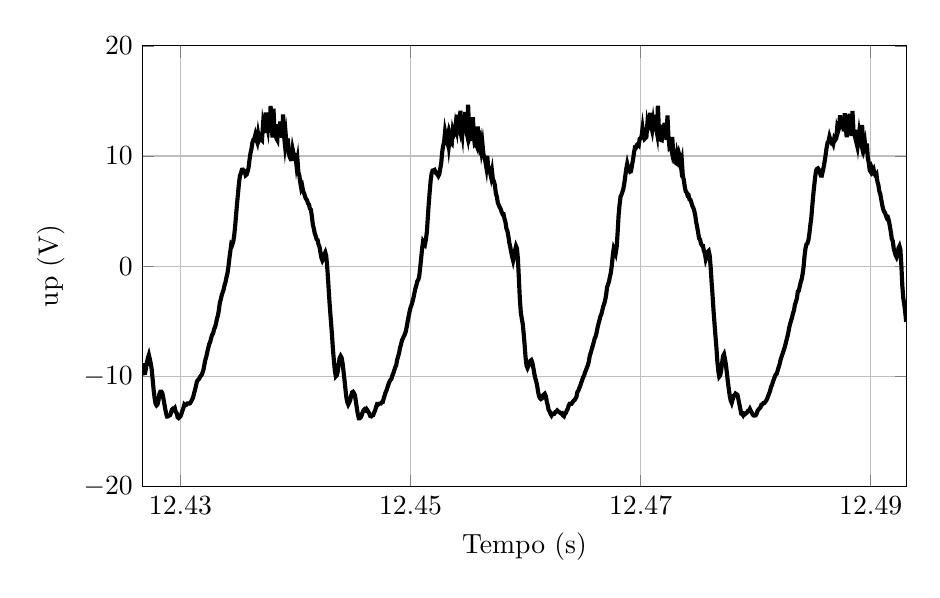
\begin{tikzpicture}

\begin{axis}[%
width=0.8\textwidth,
height=0.461611624834875\textwidth,
scale only axis,
xmin=12.4267,
xmax=12.4931,
xtick={12.43, 12.45, 12.47, 12.49},
xlabel={Tempo (s)},
xmajorgrids,
ymin=-20,
ymax=20,
ytick={-20, -10,   0,  10,  20},
ylabel={up (V)},
ymajorgrids,
scaled x ticks = false,
legend style={font=\footnotesize}
]
\addplot [color=black,solid,line width=1.5pt,forget plot]
  table[row sep=crcr]{12.4266666610667	-8.80980872005165\\
12.4267500010669	-9.47528186296987\\
12.4268333410671	-9.71595194051079\\
12.4269166510673	-9.69818881694053\\
12.4269999910675	-9.28116571823897\\
12.4270833310677	-8.71981679598147\\
12.4271666710679	-8.33543410332883\\
12.4272500110681	-8.05639851438301\\
12.4273333210683	-8.44076447657465\\
12.4274166610685	-8.84366347362103\\
12.4275000010688	-9.39406031934077\\
12.427583341069	-10.3351422852336\\
12.4276666510692	-11.2490277710424\\
12.4277499910694	-11.9721321030172\\
12.4278333310696	-12.4978024888939\\
12.4279166710698	-12.6320132989802\\
12.42800001107	-12.5392685716701\\
12.4280833210702	-12.2214240646547\\
12.4281666610704	-11.5876684366485\\
12.4282500010706	-11.3829320830804\\
12.4283333410708	-11.3828340642084\\
12.428416651071	-11.5135269964183\\
12.4284999910713	-11.9394214304095\\
12.4285833310715	-12.4188441626416\\
12.4286666710717	-12.9146408325806\\
12.4287500110719	-13.3751786655521\\
12.4288333210721	-13.6475026470308\\
12.4289166610723	-13.6357606914702\\
12.4290000010725	-13.5616143124692\\
12.4290833410727	-13.5335956725352\\
12.4291666510729	-13.3420604610174\\
12.4292499910731	-13.0241567110946\\
12.4293333310733	-12.9355137878632\\
12.4294166710735	-12.9766551710685\\
12.4295000110738	-12.8752781941256\\
12.429583321074	-13.2158914828412\\
12.4296666610742	-13.3374889091417\\
12.4297500010744	-13.7154689012019\\
12.4298333410746	-13.7840720279976\\
12.4299166510748	-13.699507040049\\
12.429999991075	-13.6243675239249\\
12.4300833310752	-13.3844297037931\\
12.4301666710754	-13.1176743573592\\
12.4302500110756	-12.8761200499939\\
12.4303333210758	-12.5532795891221\\
12.430416661076	-12.6328165290661\\
12.4305000010763	-12.5870577655248\\
12.4305833410765	-12.4626692840814\\
12.4306666510767	-12.4627641176965\\
12.4307499910769	-12.4745655927223\\
12.4308333310771	-12.4340547804061\\
12.4309166710773	-12.2955882814011\\
12.4310000110775	-12.1121301162084\\
12.4310833210777	-11.9584558581051\\
12.4311666610779	-11.5833203707308\\
12.4312500010781	-11.2680732642894\\
12.4313333410783	-10.9209103284314\\
12.4314166510785	-10.5079571396152\\
12.4314999910788	-10.3459531551036\\
12.431583331079	-10.274432725685\\
12.4316666710792	-10.1109744218451\\
12.4317500110794	-9.96408178559859\\
12.4318333210796	-9.87537564802676\\
12.4319166610798	-9.66636447997055\\
12.43200000108	-9.37480957136079\\
12.4320833410802	-8.89598643087495\\
12.4321666510804	-8.46836821111052\\
12.4322499910806	-8.18737287014583\\
12.4323333310808	-7.76857904936522\\
12.432416671081	-7.40322407993946\\
12.4325000110813	-7.06309141050896\\
12.4325833210815	-6.86885114795297\\
12.4326666610817	-6.50183520134374\\
12.4327500010819	-6.23252725678643\\
12.4328333410821	-6.10653351284327\\
12.4329166510823	-5.73208850980283\\
12.4329999910825	-5.53784217376659\\
12.4330833310827	-5.22733684683276\\
12.4331666710829	-4.77530177235292\\
12.4332500110831	-4.47946926400564\\
12.4333333210833	-3.99945570205384\\
12.4334166610835	-3.32728870739631\\
12.4335000010838	-3.01931745382929\\
12.433583341084	-2.63445335397425\\
12.4336666510842	-2.37302579888952\\
12.4337499910844	-2.12217167978476\\
12.4338333310846	-1.70774812961802\\
12.4339166710848	-1.42877574239874\\
12.434000011085	-0.994361897273687\\
12.4340833210852	-0.644872123476725\\
12.4341666610854	-0.0480793313494553\\
12.4342500010856	0.717924007917058\\
12.4343333410858	1.37362801542235\\
12.434416651086	2.02152515660813\\
12.4344999910863	1.93404622268036\\
12.4345833310865	2.1955964429569\\
12.4346666710867	2.78088207196353\\
12.4347500110869	3.61319295233917\\
12.4348333210871	4.65749806611505\\
12.4349166610873	5.68635834647359\\
12.4350000010875	6.59524811587383\\
12.4350833410877	7.53682408784159\\
12.4351666510879	8.19081643441663\\
12.4352499910881	8.43131227904881\\
12.4353333310883	8.75123892928898\\
12.4354166710885	8.76126217000512\\
12.4355000110888	8.58327454478185\\
12.435583321089	8.60802379805769\\
12.4356666610892	8.24646616066755\\
12.4357500010894	8.3203621071427\\
12.4358333410896	8.60718420483981\\
12.4359166510898	8.93958763852065\\
12.43599999109	9.65890066043226\\
12.4360833310902	10.2598885490058\\
12.4361666710904	10.6335784654577\\
12.4362500110906	11.2041578809017\\
12.4363333210908	11.4748033305402\\
12.436416661091	11.5544977461617\\
12.4365000010913	11.9029711378049\\
12.4365833410915	11.533633106971\\
12.4366666510917	11.2737472734863\\
12.4367499910919	11.9769806106023\\
12.4368333310921	11.4627741310366\\
12.4369166710923	11.6677378324315\\
12.4370000110925	11.5348476735675\\
12.4370833210927	11.446483881284\\
12.4371666610929	12.7422279540834\\
12.4372500010931	12.2185853812396\\
12.4373333410933	12.2571051185551\\
12.4374166510935	13.9409731200115\\
12.4374999910938	12.9114382382964\\
12.437583331094	12.4761550306426\\
12.4376666710942	13.7763676560752\\
12.4377500110944	12.7218440678616\\
12.4378333210946	14.5295118986927\\
12.4379166610948	12.5472707479658\\
12.438000001095	11.6867713804904\\
12.4380833410952	14.2832729153501\\
12.4381666510954	12.2930015683006\\
12.4382499910956	12.2493494285585\\
12.4383333310958	11.6145099316738\\
12.438416671096	11.4532750804882\\
12.4385000110963	12.8765333392056\\
12.4385833210965	11.917701047639\\
12.4386666610967	13.1261987179452\\
12.4387500010969	12.2864198181739\\
12.4388333410971	11.6679645646603\\
12.4389166510973	13.7631971110733\\
12.4389999910975	11.847043697222\\
12.4390833310977	10.9870704417211\\
12.4391666710979	11.7122494976925\\
12.4392500110981	10.6894452276072\\
12.4393333210983	11.5832750106622\\
12.4394166610985	10.1948612158635\\
12.4395000010988	9.92380792275027\\
12.439583341099	9.70382577543722\\
12.4396666510992	9.71385187317994\\
12.4397499910994	10.60470038907\\
12.4398333310996	10.1918824733612\\
12.4399166710998	10.1140269741963\\
12.4400000111	9.9901745829543\\
12.4400833211002	9.17543456168561\\
12.4401666611004	9.67138940260628\\
12.4402500011006	8.50672068908888\\
12.4403333411008	8.22176605428748\\
12.440416651101	7.57085176855137\\
12.4404999911013	7.04947316795797\\
12.4405833311015	7.24664799980959\\
12.4406666711017	6.77798315162836\\
12.4407500111019	6.60449634841452\\
12.4408333211021	6.29841129228866\\
12.4409166611023	6.10222574528888\\
12.4410000011025	5.99350913961882\\
12.4410833411027	5.70405925339769\\
12.4411666511029	5.60016745118408\\
12.4412499911031	5.22094590886994\\
12.4413333311033	5.12276567675533\\
12.4414166711035	4.55875934276016\\
12.4415000111038	3.81024693980174\\
12.441583321104	3.43292532711847\\
12.4416666611042	3.00064041225794\\
12.4417500011044	2.74637889155888\\
12.4418333411046	2.43722461107649\\
12.4419166511048	2.37962531373624\\
12.441999991105	1.95812136731988\\
12.4420833311052	1.75000290543025\\
12.4421666711054	1.23885024943934\\
12.4422500111056	0.766199510840753\\
12.4423333211058	0.530741264236811\\
12.442416661106	0.711571116704074\\
12.4425000011063	1.06991480303069\\
12.4425833411065	1.25011367051053\\
12.4426666511067	0.931931880935931\\
12.4427499911069	-0.00487537797634836\\
12.4428333311071	-1.28641960409488\\
12.4429166711073	-2.70860894589779\\
12.4430000111075	-3.9581556719509\\
12.4430833211077	-5.07321136708899\\
12.4431666611079	-6.20993615085097\\
12.4432500011081	-7.51466245271127\\
12.4433333411083	-8.56332311511743\\
12.4434166511085	-9.46555287366213\\
12.4434999911088	-10.0095808965784\\
12.443583331109	-9.91665741846503\\
12.4436666711092	-9.58647245611611\\
12.4437500111094	-8.91188047585344\\
12.4438333211096	-8.32975857223622\\
12.4439166611098	-8.1518728096492\\
12.44400000111	-8.30666967848963\\
12.4440833411102	-8.76150375955329\\
12.4441666511104	-9.50214344393857\\
12.4442499911106	-10.2728664966871\\
12.4443333311108	-11.0920751544021\\
12.444416671111	-11.8985764719121\\
12.4445000111113	-12.3378730765934\\
12.4445833211115	-12.5590886370248\\
12.4446666611117	-12.3837915928099\\
12.4447500011119	-12.179813891383\\
12.4448333411121	-11.7758921902961\\
12.4449166511123	-11.4512417153366\\
12.4449999911125	-11.397941804632\\
12.4450833311127	-11.5187266110509\\
12.4451666711129	-11.7190838363451\\
12.4452500111131	-12.3035728550331\\
12.4453333211133	-12.9188431481261\\
12.4454166611135	-13.4355405212503\\
12.4455000011138	-13.7988123578512\\
12.445583341114	-13.7986895703945\\
12.4456666511142	-13.7266687644267\\
12.4457499911144	-13.5364418863404\\
12.4458333311146	-13.2588320240131\\
12.4459166711148	-13.0821133014718\\
12.446000011115	-12.9878431701438\\
12.4460833211152	-13.0680539855691\\
12.4461666611154	-12.9575609311014\\
12.4462500011156	-13.0796366151937\\
12.4463333411158	-13.2315018592471\\
12.446416651116	-13.3948764099943\\
12.4464999911163	-13.6042717818069\\
12.4465833311165	-13.6318189343453\\
12.4466666711167	-13.5347835365449\\
12.4467500111169	-13.521348167226\\
12.4468333211171	-13.2774612500022\\
12.4469166611173	-13.1048990052744\\
12.4470000011175	-12.7851525767799\\
12.4470833411177	-12.5376086915766\\
12.4471666511179	-12.5690017717784\\
12.4472499911181	-12.4771765673625\\
12.4473333311183	-12.4747939686947\\
12.4474166711185	-12.4652598330718\\
12.4475000111188	-12.3483199330006\\
12.447583321119	-12.3306826886834\\
12.4476666611192	-11.9997498308185\\
12.4477500011194	-11.7187459636438\\
12.4478333411196	-11.4498055669635\\
12.4479166511198	-11.2570412318809\\
12.44799999112	-10.9766063486012\\
12.4480833311202	-10.7034278033143\\
12.4481666711204	-10.4910060951702\\
12.4482500111206	-10.3312747873615\\
12.4483333211208	-10.2361367646021\\
12.448416661121	-9.9280946020085\\
12.4485000011213	-9.72782996843506\\
12.4485833411215	-9.44752952644048\\
12.4486666511217	-9.18912055735661\\
12.4487499911219	-8.9960473829608\\
12.4488333311221	-8.49455075536907\\
12.4489166711223	-8.19788973235553\\
12.4490000111225	-7.89588577747323\\
12.4490833211227	-7.40642116206443\\
12.4491666611229	-7.1220561939262\\
12.4492500011231	-6.73344409305581\\
12.4493333411233	-6.55310611342255\\
12.4494166511235	-6.36626744796837\\
12.4494999911238	-6.17290065028287\\
12.449583331124	-5.92033270843906\\
12.4496666711242	-5.50103077781997\\
12.4497500111244	-4.97126149159909\\
12.4498333211246	-4.54418524517964\\
12.4499166611248	-4.11451162644473\\
12.450000001125	-3.75135597756508\\
12.4500833411252	-3.52818652177464\\
12.4501666511254	-3.20762308616003\\
12.4502499911256	-2.8816447628186\\
12.4503333311258	-2.4418308280614\\
12.450416671126	-2.04029758616538\\
12.4505000111263	-1.75342715125796\\
12.4505833211265	-1.37064523694653\\
12.4506666611267	-1.24642892277084\\
12.4507500011269	-0.935522061804332\\
12.4508333411271	-0.172072158302121\\
12.4509166511273	0.669713786578534\\
12.4509999911275	1.55163798379205\\
12.4510833311277	2.22661715952008\\
12.4511666711279	2.07975210742027\\
12.4512500111281	1.9650731505113\\
12.4513333211283	2.43222241560681\\
12.4514166611285	3.10411195974585\\
12.4515000011288	4.42683178375083\\
12.451583341129	5.72000610041901\\
12.4516666511292	6.80452895258514\\
12.4517499911294	7.81091052856272\\
12.4518333311296	8.44140712970879\\
12.4519166711298	8.67847138613707\\
12.45200001113	8.70039655891002\\
12.4520833211302	8.74359744374541\\
12.4521666611304	8.56116368994364\\
12.4522500011306	8.39787091538831\\
12.4523333411308	8.36141666295899\\
12.452416651131	8.19412112774633\\
12.4524999911313	8.36813754024423\\
12.4525833311315	8.86564647118493\\
12.4526666711317	9.38279925621948\\
12.4527500111319	10.3632659130654\\
12.4528333211321	10.9090926216897\\
12.4529166611323	11.2875726803599\\
12.4530000011325	12.2152988808232\\
12.4530833411327	11.7838809461717\\
12.4531666511329	11.4179541835787\\
12.4532499911331	11.8474560989654\\
12.4533333311333	10.971955704279\\
12.4534166711335	11.6797085147735\\
12.4535000111338	11.2118987384377\\
12.453583321134	11.1188679781901\\
12.4536666611342	12.2138560785823\\
12.4537500011344	11.85762873309\\
12.4538333411346	12.0307647706245\\
12.4539166511348	12.8060524053546\\
12.453999991135	12.4033326457496\\
12.4540833311352	13.7503526920163\\
12.4541666711354	12.8829013195506\\
12.4542500111356	12.5130117795594\\
12.4543333211358	14.1104142350192\\
12.454416661136	12.6478526704599\\
12.4545000011363	12.0494136440809\\
12.4545833411365	13.5160749552545\\
12.4546666511367	12.0596154304228\\
12.4547499911369	14.0030503629507\\
12.4548333311371	12.3421281537425\\
12.4549166711373	11.9332943483298\\
12.4550000111375	14.6481889147353\\
12.4550833211377	12.4777722180075\\
12.4551666611379	11.7706199684462\\
12.4552500011381	12.024956239541\\
12.4553333411383	11.3924842561197\\
12.4554166511385	13.5201622236473\\
12.4554999911387	11.7356760664287\\
12.455583331139	11.0510305429748\\
12.4556666711392	11.1297857822318\\
12.4557500111394	10.9121173854188\\
12.4558333211396	12.678972386139\\
12.4559166611398	11.4183750068283\\
12.45600000114	10.9604558494803\\
12.4560833411402	11.3670166739078\\
12.4561666511404	10.5553760363409\\
12.4562499911406	11.0908071964023\\
12.4563333311408	10.1689747189471\\
12.456416671141	9.90822416241703\\
12.4565000111413	9.49402400123042\\
12.4565833211415	8.9905604945525\\
12.4566666611417	10.0126535430831\\
12.4567500011419	8.95435247991683\\
12.4568333411421	8.93277601664239\\
12.4569166511423	8.47055386847136\\
12.4569999911425	8.0867944210375\\
12.4570833311427	8.57490701707301\\
12.4571666711429	7.78006322555396\\
12.4572500111431	7.71365275654285\\
12.4573333211433	7.30990293926589\\
12.4574166611435	6.58851220560956\\
12.4575000011438	6.30906338610719\\
12.457583341144	5.76306420072642\\
12.4576666511442	5.55519200755609\\
12.4577499911444	5.34594007303343\\
12.4578333311446	5.18967003479782\\
12.4579166711448	4.92694528948492\\
12.458000011145	4.71256701527926\\
12.4580833211452	4.71628372851141\\
12.4581666611454	4.29765801596722\\
12.4582500011456	3.9901230727059\\
12.4583333411458	3.41160615687878\\
12.458416651146	3.19662885544115\\
12.4584999911462	2.74379462574359\\
12.4585833311465	2.13113671795845\\
12.4586666711467	1.73677211275849\\
12.4587500111469	1.26404185982646\\
12.4588333211471	0.849339558082793\\
12.4589166611473	0.497803496000568\\
12.4590000011475	0.885165668841903\\
12.4590833411477	1.45069626427517\\
12.4591666511479	1.81858037618844\\
12.4592499911481	1.60984689093242\\
12.4593333311483	0.614950095116026\\
12.4594166711485	-1.12644846939151\\
12.4595000111488	-2.96967656296611\\
12.459583321149	-4.19591281615346\\
12.4596666611492	-4.75103340029111\\
12.4597500011494	-5.23159538256114\\
12.4598333411496	-6.11066746599213\\
12.4599166511498	-7.16852053675604\\
12.45999999115	-8.31026643786585\\
12.4600833311502	-9.03562402947178\\
12.4601666711504	-9.24355795167065\\
12.4602500111506	-9.04765974873263\\
12.4603333211508	-8.86995965041344\\
12.460416661151	-8.58806437361368\\
12.4605000011512	-8.52191457524913\\
12.4605833411515	-8.74927929874558\\
12.4606666511517	-9.19324757041546\\
12.4607499911519	-9.71181033717103\\
12.4608333311521	-10.1342842549121\\
12.4609166711523	-10.4382404715723\\
12.4610000111525	-10.8114661964703\\
12.4610833211527	-11.3845562845755\\
12.4611666611529	-11.7791299855686\\
12.4612500011531	-11.9822288260466\\
12.4613333411533	-12.0636712466722\\
12.4614166511535	-12.0061566908308\\
12.4614999911537	-11.7294454261201\\
12.461583331154	-11.6547624984645\\
12.4616666711542	-11.5795734932722\\
12.4617500111544	-11.7818629340482\\
12.4618333211546	-12.244082689732\\
12.4619166611548	-12.5920389010011\\
12.462000001155	-13.0483718474783\\
12.4620833411552	-13.1626387349973\\
12.4621666511554	-13.408287310317\\
12.4622499911556	-13.55060568945\\
12.4623333311558	-13.3915581886541\\
12.462416671156	-13.4178608435003\\
12.4625000111563	-13.3984719072791\\
12.4625833211565	-13.2415035983952\\
12.4626666611567	-13.2136948322117\\
12.4627500011569	-13.1009868720989\\
12.4628333411571	-13.1937295509218\\
12.4629166511573	-13.2309135088351\\
12.4629999911575	-13.3092065319426\\
12.4630833311577	-13.3729842262683\\
12.4631666711579	-13.3470234635039\\
12.4632500111581	-13.5482209677515\\
12.4633333211583	-13.6198753297114\\
12.4634166611585	-13.3829558528602\\
12.4635000011587	-13.3193174566661\\
12.463583341159	-13.0938468145988\\
12.4636666511592	-12.9311252941812\\
12.4637499911594	-12.6400112898177\\
12.4638333311596	-12.4800950222201\\
12.4639166711598	-12.4815135782073\\
12.46400001116	-12.4808655830348\\
12.4640833211602	-12.3490548719677\\
12.4641666611604	-12.2211436891985\\
12.4642500011606	-12.1716450668889\\
12.4643333411608	-12.0166238970407\\
12.464416651161	-11.8693464813643\\
12.4644999911613	-11.4219454741292\\
12.4645833311615	-11.3008614920505\\
12.4646666711617	-11.0678355881158\\
12.4647500111619	-10.857142065756\\
12.4648333211621	-10.5753276936546\\
12.4649166611623	-10.3623672434597\\
12.4650000011625	-10.0660755167298\\
12.4650833411627	-9.94041543396986\\
12.4651666511629	-9.64372533672869\\
12.4652499911631	-9.44052669603529\\
12.4653333311633	-9.19015991288585\\
12.4654166711635	-8.97345408287184\\
12.4655000111638	-8.64245035672755\\
12.465583321164	-8.11824380059442\\
12.4656666611642	-7.85136765940594\\
12.4657500011644	-7.53434776704537\\
12.4658333411646	-7.23844068751244\\
12.4659166511648	-6.9305932552805\\
12.465999991165	-6.57195984828398\\
12.4660833311652	-6.39365180969441\\
12.4661666711654	-6.04890502057826\\
12.4662500111656	-5.60470328438157\\
12.4663333211658	-5.25835730696038\\
12.466416661166	-4.91439134781377\\
12.4665000011662	-4.56268546620682\\
12.4665833411665	-4.36884826946402\\
12.4666666511667	-4.02517831134487\\
12.4667499911669	-3.65464946710704\\
12.4668333311671	-3.39965470206142\\
12.4669166711673	-3.0949254411905\\
12.4670000111675	-2.60156491819325\\
12.4670833211677	-1.91726130819417\\
12.4671666611679	-1.64989133804637\\
12.4672500011681	-1.38843686338962\\
12.4673333411683	-0.939869293920112\\
12.4674166511685	-0.572725249688572\\
12.4674999911688	0.125642033721624\\
12.467583331169	1.01254690621118\\
12.4676666711692	1.62646390375368\\
12.4677500111694	1.43936415830276\\
12.4678333211696	1.18254369941686\\
12.4679166611698	1.74045445440744\\
12.46800000117	3.05431948329508\\
12.4680833411702	4.59676928441736\\
12.4681666511704	5.54095935360256\\
12.4682499911706	6.29622431441983\\
12.4683333311708	6.47725302437876\\
12.468416671171	6.74143915673298\\
12.4685000111712	7.02179011978823\\
12.4685833211715	7.53211243270542\\
12.4686666611717	8.18973040925418\\
12.4687500011719	8.81250577103286\\
12.4688333411721	9.27838217319299\\
12.4689166511723	8.89638591886\\
12.4689999911725	8.78452806922592\\
12.4690833311727	8.5745166142408\\
12.4691666711729	8.62520652304537\\
12.4692500111731	9.18085662221818\\
12.4693333211733	9.62781280436946\\
12.4694166611735	10.2484067391605\\
12.4695000011738	10.7566914968479\\
12.469583341174	10.7365835331309\\
12.4696666511742	10.9923421138122\\
12.4697499911744	11.0768512105486\\
12.4698333311746	10.9801077716804\\
12.4699166711748	11.5497552991923\\
12.470000011175	11.6075381973441\\
12.4700833211752	11.8074025305912\\
12.4701666611754	12.5103786578506\\
12.4702500011756	11.8483868454194\\
12.4703333411758	11.5472602004709\\
12.470416651176	11.6311294962531\\
12.4704999911763	11.7119758213236\\
12.4705833311765	12.907406860629\\
12.4706666711767	12.4772581014314\\
12.4707500111769	12.5336217999463\\
12.4708333211771	13.9140950735094\\
12.4709166611773	12.7030151982255\\
12.4710000011775	12.3210210461759\\
12.4710833411777	13.0224859863427\\
12.4711666511779	12.3011114823547\\
12.4712499911781	13.7372603493848\\
12.4713333311783	12.5915505408493\\
12.4714166711785	12.1128704382023\\
12.4715000111787	14.5663870449859\\
12.471583321179	12.5141832222818\\
12.4716666611792	12.2377952628186\\
12.4717500011794	11.4707793460266\\
12.4718333411796	11.4337612170767\\
12.4719166511798	12.8266467425629\\
12.47199999118	11.9359890916564\\
12.4720833311802	13.0053563079461\\
12.4721666711804	12.0914375219053\\
12.4722500111806	11.4854092339492\\
12.4723333211808	13.6732320858943\\
12.472416661181	11.7636795173823\\
12.4725000011813	10.8781224086531\\
12.4725833411815	11.0221385855338\\
12.4726666511817	10.6097876876057\\
12.4727499911819	11.7289913525952\\
12.4728333311821	10.2380635408207\\
12.4729166711823	9.66070784843874\\
12.4730000111825	9.42072728026718\\
12.4730833211827	9.35745960356864\\
12.4731666611829	10.1596765666077\\
12.4732500011831	9.77111495449099\\
12.4733333411833	10.2147040895664\\
12.4734166511835	9.89993798445971\\
12.4734999911838	9.14071279452701\\
12.473583331184	9.54525346856092\\
12.4736666711842	8.21171475136582\\
12.4737500111844	7.83791376153713\\
12.4738333211846	7.2308073720362\\
12.4739166611848	6.80084154016418\\
12.474000001185	6.69287552886893\\
12.4740833411852	6.4148860690168\\
12.4741666511854	6.44052133608171\\
12.4742499911856	6.05843389575975\\
12.4743333311858	6.02120811440711\\
12.474416671186	5.75085722110202\\
12.4745000111862	5.45819979143173\\
12.4745833211865	5.28881581413422\\
12.4746666611867	5.0104970461369\\
12.4747500011869	4.58884418079446\\
12.4748333411871	3.97954393577238\\
12.4749166511873	3.54588223847928\\
12.4749999911875	3.03961111122504\\
12.4750833311877	2.52912350154224\\
12.4751666711879	2.42344645318853\\
12.4752500111881	2.0290674476319\\
12.4753333211883	1.87524894696878\\
12.4754166611885	1.85220398615231\\
12.4755000011888	1.37923441279799\\
12.475583341189	1.17733247781833\\
12.4756666511892	0.628878525027252\\
12.4757499911894	0.884261899445867\\
12.4758333311896	1.3045999039936\\
12.4759166711898	1.39272143155435\\
12.47600001119	0.991537787523368\\
12.4760833211902	-0.0215186179041303\\
12.4761666611904	-1.406092844045\\
12.4762500011906	-2.59683623111054\\
12.4763333411908	-3.96735135218328\\
12.476416651191	-5.116908756765\\
12.4764999911913	-6.2731832457166\\
12.4765833311915	-7.30490208315636\\
12.4766666711917	-8.60447578321923\\
12.4767500111919	-9.48632588120948\\
12.4768333211921	-10.027876373356\\
12.4769166611923	-9.91347600314586\\
12.4770000011925	-9.4577704323333\\
12.4770833411927	-8.77628781991244\\
12.4771666511929	-8.15227066500466\\
12.4772499911931	-7.99253575154157\\
12.4773333311933	-8.44643111984694\\
12.4774166711935	-8.97482411591112\\
12.4775000111938	-9.7138061745542\\
12.477583321194	-10.4897342792488\\
12.4776666611942	-11.1481434041145\\
12.4777500011944	-11.7915200409387\\
12.4778333411946	-12.1991647749555\\
12.4779166511948	-12.4109091011613\\
12.477999991195	-12.109600569518\\
12.4780833311952	-11.7626055887487\\
12.4781666711954	-11.7118286894543\\
12.4782500111956	-11.5621569649419\\
12.4783333211958	-11.6251891039761\\
12.478416661196	-11.6780996945905\\
12.4785000011963	-12.0922332590267\\
12.4785833411965	-12.5263722308086\\
12.4786666511967	-12.9698267533357\\
12.4787499911969	-13.3816163181811\\
12.4788333311971	-13.3897578242488\\
12.4789166711973	-13.5369527096989\\
12.4790000111975	-13.382934633618\\
12.4790833211977	-13.4256223047657\\
12.4791666611979	-13.3331182079952\\
12.4792500011981	-13.281793793401\\
12.4793333411983	-13.1313482932961\\
12.4794166511985	-13.1296719717966\\
12.4794999911988	-12.9607178138879\\
12.479583331199	-13.1492820889567\\
12.4796666711992	-13.2877685610403\\
12.4797500111994	-13.4819200863924\\
12.4798333211996	-13.5502692216092\\
12.4799166611998	-13.5546939333325\\
12.4800000012	-13.5395358540222\\
12.4800833412002	-13.3963145714666\\
12.4801666512004	-13.1259137024704\\
12.4802499912006	-13.0047384647782\\
12.4803333312008	-12.9084204724718\\
12.480416671201	-12.823084102529\\
12.4805000112013	-12.5738569854204\\
12.4805833212015	-12.5555474457639\\
12.4806666612017	-12.4342696000533\\
12.4807500012019	-12.433473879802\\
12.4808333412021	-12.3266233027352\\
12.4809166512023	-12.1969977524311\\
12.4809999912025	-12.0254132876043\\
12.4810833312027	-11.7958895582822\\
12.4811666712029	-11.5611494885673\\
12.4812500112031	-11.3435906597586\\
12.4813333212033	-10.9625439706676\\
12.4814166612035	-10.8004048811767\\
12.4815000012038	-10.5016478619553\\
12.481583341204	-10.2644671099236\\
12.4816666512042	-10.0161118035826\\
12.4817499912044	-9.81623833458744\\
12.4818333312046	-9.7625934503163\\
12.4819166712048	-9.45661301207305\\
12.482000011205	-9.16268469532169\\
12.4820833212052	-8.89905795837933\\
12.4821666612054	-8.49054371197992\\
12.4822500012056	-8.21953508969576\\
12.4823333412058	-7.98315365071645\\
12.482416651206	-7.71038133090706\\
12.4824999912063	-7.4529705692174\\
12.4825833312065	-7.13426170342368\\
12.4826666712067	-6.76951884271848\\
12.4827500112069	-6.43606215498212\\
12.4828333212071	-6.05312167294301\\
12.4829166612073	-5.57684837478873\\
12.4830000012075	-5.21944850978692\\
12.4830833412077	-4.92398248935899\\
12.4831666512079	-4.6457179961634\\
12.4832499912081	-4.24658611104006\\
12.4833333312083	-4.00062718909633\\
12.4834166712085	-3.47722065991248\\
12.4835000112088	-3.23351643963629\\
12.483583321209	-2.93040729743567\\
12.4836666612092	-2.28939027564748\\
12.4837500012094	-2.22695442385704\\
12.4838333412096	-1.83586108700245\\
12.4839166512098	-1.44416805918544\\
12.48399999121	-1.17856379833167\\
12.4840833312102	-0.711209696052085\\
12.4841666712104	-0.0506684547079084\\
12.4842500112106	0.919646999918614\\
12.4843333212108	1.62398814503424\\
12.484416661211	1.99418287081003\\
12.4845000012113	2.06247501981271\\
12.4845833412115	2.33786185448729\\
12.4846666512117	2.92157959599211\\
12.4847499912119	3.70211691291694\\
12.4848333312121	4.347767911663\\
12.4849166712123	5.37418115998709\\
12.4850000112125	6.40413371423558\\
12.4850833212127	7.24025689487826\\
12.4851666612129	8.02354236364482\\
12.4852500012131	8.67630979018551\\
12.4853333412133	8.82911147842963\\
12.4854166512135	8.87832711450855\\
12.4854999912138	8.737398109982\\
12.485583331214	8.47473364451139\\
12.4856666712142	8.22600850786485\\
12.4857500112144	8.21934495189464\\
12.4858333212146	8.60758907914801\\
12.4859166612148	9.02085358046543\\
12.486000001215	9.52218151092899\\
12.4860833412152	10.1070184259932\\
12.4861666512154	10.7412938135622\\
12.4862499912156	11.2061176849677\\
12.4863333312158	11.3294783758019\\
12.486416671216	11.7514914265723\\
12.4865000112163	11.4591307697683\\
12.4865833212165	11.250300775923\\
12.4866666612167	11.3693544206278\\
12.4867500012169	11.1291317822897\\
12.4868333412171	11.5942788608121\\
12.4869166512173	11.4484210624171\\
12.4869999912175	11.5764219713234\\
12.4870833312177	12.5140694138968\\
12.4871666712179	12.2410554380488\\
12.4872500112181	12.5404514086395\\
12.4873333212183	13.6858431823592\\
12.4874166612185	12.8534290765573\\
12.4875000012188	13.0382925421992\\
12.487583341219	13.1388496714541\\
12.4876666512192	12.2345953330228\\
12.4877499912194	13.8893400847112\\
12.4878333312196	12.5584122103347\\
12.4879166712198	11.7005617071317\\
12.48800001122	13.2434484162305\\
12.4880833212202	12.2701203089539\\
12.4881666612204	13.8267147393615\\
12.4882500012206	12.3756345646882\\
12.4883333412208	11.8259697963962\\
12.488416651221	14.0766154824187\\
12.4884999912213	12.3761138958318\\
12.4885833312215	12.0616595490822\\
12.4886666712217	11.616085037111\\
12.4887500112219	11.2553466121559\\
12.4888333212221	12.3668415687102\\
12.4889166612223	11.3893563395562\\
12.4890000012225	12.1174480539385\\
12.4890833412227	11.5752203340336\\
12.4891666512229	11.1786590942741\\
12.4892499912231	12.8045195198831\\
12.4893333312233	11.3667285303852\\
12.4894166712235	10.7538114619235\\
12.4895000112238	11.148318153922\\
12.489583321224	10.2538996961057\\
12.4896666612242	11.1300786185441\\
12.4897500012244	9.81084319866057\\
12.4898333412246	9.35810771338559\\
12.4899166512248	8.70690714795391\\
12.489999991225	8.56491379218895\\
12.4900833312252	8.89209693433684\\
12.4901666712254	8.63543213427434\\
12.4902500112256	8.78579294469572\\
12.4903333212258	8.35760780919457\\
12.490416661226	8.21966579566965\\
12.4905000012263	8.33900683476184\\
12.4905833412265	7.66850965677854\\
12.4906666512267	7.39148217204075\\
12.4907499912269	6.79854847936098\\
12.4908333312271	6.54189521988972\\
12.4909166712273	6.05529451654625\\
12.4910000112275	5.577945754516\\
12.4910833212277	5.18053569965904\\
12.4911666612279	4.94418722809988\\
12.4912500012281	4.83855896840802\\
12.4913333412283	4.56144303952203\\
12.4914166512285	4.34643593249498\\
12.4914999912288	4.40979403250769\\
12.491583331229	4.11486695971276\\
12.4916666712292	3.62568400989959\\
12.4917500112294	3.11497464549468\\
12.4918333212296	2.50035418733049\\
12.4919166612298	2.27861193746185\\
12.49200000123	1.63253941283155\\
12.4920833412302	1.30556711454455\\
12.4921666512304	0.994482126241465\\
12.4922499912306	0.816726024711957\\
12.4923333312308	1.06635073938111\\
12.492416671231	1.64350694727793\\
12.4925000112313	1.8228632642067\\
12.4925833212315	1.49919274148553\\
12.4926666612317	0.0668635375389842\\
12.4927500012319	-1.78011818768771\\
12.4928333412321	-2.90652492150646\\
12.4929166512323	-3.45784521759843\\
12.4929999912325	-4.1547309779736\\
12.4930833312327	-5.05500190666392\\
};
\end{axis}
\end{tikzpicture}%}}
    \end{figure}
    \end{small}
    \vfill
  }

  \frame{
    \frametitle{\insertsection}
    \vfill
    \begin{small}
    \begin{figure}[htb]
      \centering
      \raisebox{-0.5\height}{
        %\def\svgwidth{0.8\linewidth}
        \resizebox{0.9\linewidth}{!}{% This file was created by matlab2tikz v0.4.7 running on MATLAB 7.14.
% Copyright (c) 2008--2014, Nico Schlömer <nico.schloemer@gmail.com>
% All rights reserved.
% Minimal pgfplots version: 1.3
% 
% The latest updates can be retrieved from
%   http://www.mathworks.com/matlabcentral/fileexchange/22022-matlab2tikz
% where you can also make suggestions and rate matlab2tikz.
% 
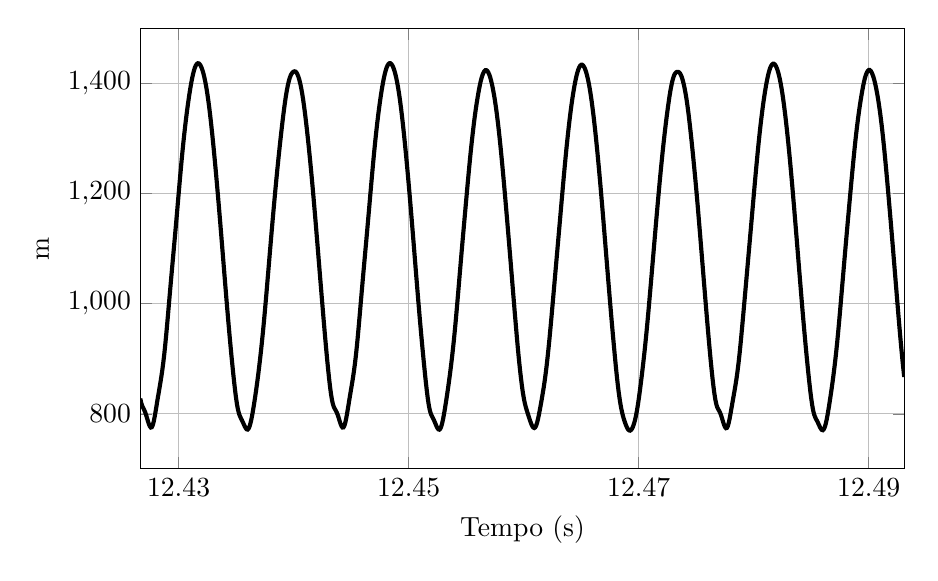
\begin{tikzpicture}

\begin{axis}[%
width=0.8\textwidth,
height=0.461611624834875\textwidth,
scale only axis,
xmin=12.4267,
xmax=12.4931,
xtick={12.43, 12.45, 12.47, 12.49},
xlabel={Tempo (s)},
xmajorgrids,
ymin=700,
ymax=1500,
ytick={ 800, 1000, 1200, 1400},
ylabel={m},
ymajorgrids,
scaled x ticks = false,
legend style={font=\footnotesize}
]
\addplot [color=black,solid,line width=1.5pt,forget plot]
  table[row sep=crcr]{12.4266666610667	827.741097437338\\
12.4267500010669	820.095895950887\\
12.4268333410671	814.789713852944\\
12.4269166510673	810.926617961449\\
12.4269999910675	807.531909658705\\
12.4270833310677	803.534657688938\\
12.4271666710679	798.570400861033\\
12.4272500110681	792.872551099854\\
12.4273333210683	786.933201603522\\
12.4274166610685	781.548953727111\\
12.4275000010688	777.383993988708\\
12.427583341069	775.212590048016\\
12.4276666510692	775.723182541313\\
12.4277499910694	779.252927661133\\
12.4278333310696	785.604996188925\\
12.4279166710698	794.216199083165\\
12.42800001107	804.222797671565\\
12.4280833210702	814.841893365837\\
12.4281666610704	825.451131277664\\
12.4282500010706	835.741846133046\\
12.4283333410708	845.973716436484\\
12.428416651071	856.35976521968\\
12.4284999910713	867.309746566374\\
12.4285833310715	879.243199917306\\
12.4286666710717	892.496036836965\\
12.4287500110719	907.305876143824\\
12.4288333210721	923.833482695955\\
12.4289166610723	941.838096425996\\
12.4290000010725	960.957851040641\\
12.4290833410727	980.817641301398\\
12.4291666510729	1000.92579027159\\
12.4292499910731	1020.98887736596\\
12.4293333310733	1040.82790546728\\
12.4294166710735	1060.40024855815\\
12.4295000110738	1079.75456804226\\
12.429583321074	1099.0191725966\\
12.4296666610742	1118.36698724123\\
12.4297500010744	1137.94421493114\\
12.4298333410746	1157.81044004841\\
12.4299166510748	1177.95550333431\\
12.429999991075	1198.19298823851\\
12.4300833310752	1218.29986903888\\
12.4301666710754	1237.99391156711\\
12.4302500110756	1257.03965366303\\
12.4303333210758	1275.2802927645\\
12.430416661076	1292.60397220553\\
12.4305000010763	1308.93102938394\\
12.4305833410765	1324.3132043524\\
12.4306666510767	1338.789220191\\
12.4307499910769	1352.41966044896\\
12.4308333310771	1365.23484828857\\
12.4309166710773	1377.23930383278\\
12.4310000110775	1388.42263963318\\
12.4310833210777	1398.70675975138\\
12.4311666610779	1407.96337654268\\
12.4312500010781	1416.09623822161\\
12.4313333410783	1422.96732743883\\
12.4314166510785	1428.48779478504\\
12.4314999910788	1432.59031029069\\
12.431583331079	1435.19998651791\\
12.4316666710792	1436.36131728105\\
12.4317500110794	1436.1788349605\\
12.4318333210796	1434.72821646989\\
12.4319166610798	1432.08090450769\\
12.43200000108	1428.27429119471\\
12.4320833410802	1423.32022496969\\
12.4321666510804	1417.2488286865\\
12.4322499910806	1409.97208244128\\
12.4323333310808	1401.49399340179\\
12.432416671081	1391.8146768497\\
12.4325000110813	1380.97245914504\\
12.4325833210815	1368.90536691772\\
12.4326666610817	1355.62218915142\\
12.4327500010819	1341.22557184323\\
12.4328333410821	1325.78212036367\\
12.4329166510823	1309.41365147623\\
12.4329999910825	1292.27124570155\\
12.4330833310827	1274.4661679459\\
12.4331666710829	1256.06850172968\\
12.4332500110831	1237.13468343795\\
12.4333333210833	1217.6098075732\\
12.4334166610835	1197.59851895734\\
12.4335000010838	1177.18560792883\\
12.433583341084	1156.33397153088\\
12.4336666510842	1135.18077956483\\
12.4337499910844	1113.80397887541\\
12.4338333310846	1092.2871389759\\
12.4339166710848	1070.75090269941\\
12.434000011085	1049.22783313728\\
12.4340833210852	1027.83099933397\\
12.4341666610854	1006.65321068067\\
12.4342500010856	985.851684622578\\
12.4343333410858	965.521923344282\\
12.434416651086	945.793461351915\\
12.4344999910863	926.736507780411\\
12.4345833310865	908.242108007742\\
12.4346666710867	890.410089121622\\
12.4347500110869	873.280735003904\\
12.4348333210871	857.044306890318\\
12.4349166610873	841.931831107451\\
12.4350000010875	828.254107995106\\
12.4350833410877	816.586761974033\\
12.4351666510879	807.370424743281\\
12.4352499910881	800.617312318397\\
12.4353333310883	795.766117977876\\
12.4354166710885	792.133431931995\\
12.4355000110888	788.67407601778\\
12.435583321089	785.036720946653\\
12.4356666610892	781.164619722054\\
12.4357500010894	777.306428243987\\
12.4358333410896	774.081134183963\\
12.4359166510898	771.972845714799\\
12.43599999109	771.535385968658\\
12.4360833310902	773.238704916023\\
12.4361666710904	777.061808044983\\
12.4362500110906	782.964542520149\\
12.4363333210908	790.618980537315\\
12.436416661091	799.683895751156\\
12.4365000010913	809.750713638863\\
12.4365833410915	820.717293780883\\
12.4366666510917	832.202736682772\\
12.4367499910919	844.224371129791\\
12.4368333310921	857.003722168216\\
12.4369166710923	870.329419874382\\
12.4370000110925	884.446595030164\\
12.4370833210927	899.290057853971\\
12.4371666610929	914.848786975554\\
12.4372500010931	931.351604497147\\
12.4373333410933	948.597452012743\\
12.4374166510935	966.688862867412\\
12.4374999910938	985.987403945112\\
12.437583331094	1005.75444318955\\
12.4376666710942	1025.99430552504\\
12.4377500110944	1046.76157817486\\
12.4378333210946	1067.4259239401\\
12.4379166610948	1088.1985403401\\
12.438000001095	1108.8235339465\\
12.4380833410952	1129.19850789744\\
12.4381666510954	1149.19605692304\\
12.4382499910956	1168.7851861842\\
12.4383333310958	1188.02075779615\\
12.438416671096	1207.04928237006\\
12.4385000110963	1225.53098458671\\
12.4385833210965	1243.2769333336\\
12.4386666610967	1260.5488986023\\
12.4387500010969	1277.18135917142\\
12.4388333410971	1293.48189076332\\
12.4389166510973	1309.19964948709\\
12.4389999910975	1324.42768433414\\
12.4390833310977	1338.990901255\\
12.4391666710979	1352.84353321745\\
12.4392500110981	1365.73457668121\\
12.4393333210983	1377.52134103604\\
12.4394166610985	1387.56680376203\\
12.4395000010988	1396.5668867192\\
12.439583341099	1403.95586926678\\
12.4396666510992	1409.98227941702\\
12.4397499910994	1414.55401458886\\
12.4398333310996	1417.74881103278\\
12.4399166710998	1419.97728930639\\
12.4400000111	1421.27523767725\\
12.4400833211002	1421.76551624367\\
12.4401666611004	1421.24995424429\\
12.4402500011006	1419.36501287054\\
12.4403333411008	1416.27936056642\\
12.440416651101	1411.81044300801\\
12.4404999911013	1406.13506257849\\
12.4405833311015	1399.11534677474\\
12.4406666711017	1390.60982541882\\
12.4407500111019	1380.75537774632\\
12.4408333211021	1369.60187691527\\
12.4409166611023	1357.21869669722\\
12.4410000011025	1343.70162289447\\
12.4410833411027	1329.22427007339\\
12.4411666511029	1313.91574792721\\
12.4412499911031	1297.8875606514\\
12.4413333311033	1281.21764727774\\
12.4414166711035	1263.80886919676\\
12.4415000111038	1245.80467182332\\
12.441583321104	1227.22307578643\\
12.4416666611042	1207.99789219666\\
12.4417500011044	1188.15500494246\\
12.4418333411046	1167.81933938726\\
12.4419166511048	1147.10430684935\\
12.441999991105	1126.04051162687\\
12.4420833311052	1104.83139594918\\
12.4421666711054	1083.38390040498\\
12.4422500111056	1061.97017642496\\
12.4423333211058	1040.58946037402\\
12.442416661106	1019.36318901171\\
12.4425000011063	998.269666698926\\
12.4425833411065	977.400590155302\\
12.4426666511067	956.874715132242\\
12.4427499911069	936.810259096241\\
12.4428333311071	917.308577347969\\
12.4429166711073	898.569267322168\\
12.4430000111075	880.802668309645\\
12.4430833211077	864.195359843596\\
12.4431666611079	849.106586838205\\
12.4432500011081	836.030317561778\\
12.4433333411083	825.453554220401\\
12.4434166511085	817.654473915795\\
12.4434999911088	812.329876588065\\
12.443583331109	808.923824187537\\
12.4436666711092	806.008944046804\\
12.4437500111094	802.659919157075\\
12.4438333211096	798.175661311404\\
12.4439166611098	792.782813321945\\
12.44400000111	787.037307698387\\
12.4440833411102	781.698687880609\\
12.4441666511104	777.507510285943\\
12.4442499911106	775.227587319546\\
12.4443333311108	775.462974787333\\
12.444416671111	778.561515722591\\
12.4445000111113	784.648332596099\\
12.4445833211115	792.983975655271\\
12.4446666611117	802.893786220521\\
12.4447500011119	813.479260964258\\
12.4448333411121	824.162406814279\\
12.4449166511123	834.655734617157\\
12.4449999911125	844.99473445013\\
12.4450833311127	855.491353549541\\
12.4451666711129	866.473325160077\\
12.4452500111131	878.348443655971\\
12.4453333211133	891.555951415168\\
12.4454166611135	906.387049641545\\
12.4455000011138	922.902388727221\\
12.445583341114	941.015464202883\\
12.4456666511142	960.280165987799\\
12.4457499911144	980.278253638775\\
12.4458333311146	1000.52481126517\\
12.4459166711148	1020.68780404572\\
12.446000011115	1040.61360201563\\
12.4460833211152	1060.24562698184\\
12.4461666611154	1079.65293080543\\
12.4462500011156	1098.96526967053\\
12.4463333411158	1118.31116270589\\
12.446416651116	1137.82423728104\\
12.4464999911163	1157.55800085624\\
12.4465833311165	1177.50982929005\\
12.4466666711167	1197.57044377294\\
12.4467500111169	1217.54021281406\\
12.4468333211171	1237.18954255255\\
12.4469166611173	1256.28298597685\\
12.4470000011175	1274.64469117472\\
12.4470833411177	1292.1731978775\\
12.4471666511179	1308.76561466547\\
12.4472499911181	1324.38879610796\\
12.4473333311183	1339.04975153137\\
12.4474166711185	1352.8100918808\\
12.4475000111188	1365.69749454324\\
12.447583321119	1377.72604342916\\
12.4476666611192	1388.85113728634\\
12.4477500011194	1399.0473464387\\
12.4478333411196	1408.19985905327\\
12.4479166511198	1416.19504498952\\
12.44799999112	1422.93304470509\\
12.4480833311202	1428.3514746712\\
12.4481666711204	1432.44578719174\\
12.4482500111206	1435.14283758485\\
12.4483333211208	1436.4521636122\\
12.448416661121	1436.34595831135\\
12.4485000011213	1434.99484394118\\
12.4485833411215	1432.40506743065\\
12.4486666511217	1428.67185554204\\
12.4487499911219	1423.73986078682\\
12.4488333311221	1417.62543810378\\
12.4489166711223	1410.35891709851\\
12.4490000111225	1401.83040266344\\
12.4490833211227	1392.07479206239\\
12.4491666611229	1381.09229537881\\
12.4492500011231	1368.9202668744\\
12.4493333411233	1355.64670721855\\
12.4494166511235	1341.26525360108\\
12.4494999911238	1325.8949508955\\
12.449583331124	1309.63345294254\\
12.4496666711242	1292.58025749484\\
12.4497500111244	1274.85596490394\\
12.4498333211246	1256.48723186019\\
12.4499166611248	1237.50965355697\\
12.450000001125	1217.97742173207\\
12.4500833411252	1197.92016394709\\
12.4501666511254	1177.38653919141\\
12.4502499911256	1156.49217671019\\
12.4503333311258	1135.29114949337\\
12.450416671126	1113.87779886622\\
12.4505000111263	1092.31857499515\\
12.4505833211265	1070.69757218393\\
12.4506666611267	1049.13882985673\\
12.4507500011269	1027.69597891559\\
12.4508333411271	1006.5075984292\\
12.4509166511273	985.762347243644\\
12.4509999911275	965.588704302176\\
12.4510833311277	946.037283522057\\
12.4511666711279	927.092803798536\\
12.4512500111281	908.579437462582\\
12.4513333211283	890.58368008044\\
12.4514166611285	873.204178572414\\
12.4515000011288	856.653021436493\\
12.451583341129	841.289452470191\\
12.4516666511292	827.573803756238\\
12.4517499911294	816.038894032171\\
12.4518333311296	807.217734942509\\
12.4519166711298	801.002107905529\\
12.45200001113	796.711064806706\\
12.4520833211302	793.391683918333\\
12.4521666611304	789.982511816501\\
12.4522500011306	786.14871486844\\
12.4523333411308	781.944156939817\\
12.452416651131	777.760699923342\\
12.4524999911313	774.205462884819\\
12.4525833311315	771.866497081067\\
12.4526666711317	771.295722817113\\
12.4527500111319	772.843385749458\\
12.4528333211321	776.942139919071\\
12.4529166611323	783.132023804767\\
12.4530000011325	791.142834624913\\
12.4530833411327	800.780470194386\\
12.4531666511329	811.141074162686\\
12.4532499911331	822.070550117374\\
12.4533333311333	833.59595421518\\
12.4534166711335	845.355740897334\\
12.4535000111338	857.834148752375\\
12.453583321134	870.808132600359\\
12.4536666611342	884.469763675553\\
12.4537500011344	898.99480745666\\
12.4538333411346	914.315903782546\\
12.4539166511348	930.615663337275\\
12.453999991135	948.109285145477\\
12.4540833311352	966.507674545694\\
12.4541666711354	986.136311143964\\
12.4542500111356	1006.25617235926\\
12.4543333211358	1026.73340350915\\
12.454416661136	1047.57470710905\\
12.4545000011363	1068.14725095621\\
12.4545833411365	1088.53921537767\\
12.4546666511367	1108.70676087484\\
12.4547499911369	1128.56384649107\\
12.4548333311371	1148.23604178129\\
12.4549166711373	1167.87559105427\\
12.4550000111375	1187.33638158841\\
12.4550833211377	1206.74107076404\\
12.4551666611379	1225.77225132088\\
12.4552500011381	1244.38983753406\\
12.4553333411383	1262.52573164553\\
12.4554166511385	1279.83789563384\\
12.4554999911387	1295.94335124731\\
12.455583331139	1311.42443535158\\
12.4556666711392	1326.06167259958\\
12.4557500111394	1339.88700128532\\
12.4558333211396	1352.6005043193\\
12.4559166611398	1364.13922089385\\
12.45600000114	1374.9532652823\\
12.4560833411402	1385.00820196287\\
12.4561666511404	1394.24022223787\\
12.4562499911406	1402.43403851284\\
12.4563333311408	1409.20652753693\\
12.456416671141	1414.84339339695\\
12.4565000111413	1419.09407868145\\
12.4565833211415	1422.14355623002\\
12.4566666611417	1423.85967420234\\
12.4567500011419	1423.84588038744\\
12.4568333411421	1422.66079484077\\
12.4569166511423	1420.04983045166\\
12.4569999911425	1416.32065805189\\
12.4570833311427	1411.30208328833\\
12.4571666711429	1404.96050422579\\
12.4572500111431	1397.61705921751\\
12.4573333211433	1389.11732228323\\
12.4574166611435	1379.56154008881\\
12.4575000011438	1369.00606973695\\
12.457583341144	1357.26240794321\\
12.4576666511442	1344.39926944254\\
12.4577499911444	1330.35535100774\\
12.4578333311446	1315.19231232904\\
12.4579166711448	1299.07277758794\\
12.458000011145	1282.13629082999\\
12.4580833211452	1264.40173734034\\
12.4581666611454	1245.92018442804\\
12.4582500011456	1226.84608642218\\
12.4583333411458	1207.25733605996\\
12.458416651146	1187.339534144\\
12.4584999911462	1167.02293636942\\
12.4585833311465	1146.54005493564\\
12.4586666711467	1125.81621901712\\
12.4587500111469	1104.94008015697\\
12.4588333211471	1083.86310365944\\
12.4589166611473	1062.68159688948\\
12.4590000011475	1041.42223371659\\
12.4590833411477	1020.07505204605\\
12.4591666511479	998.780834051415\\
12.4592499911481	977.774090191602\\
12.4593333311483	957.177735575863\\
12.4594166711485	937.113241326438\\
12.4595000111488	917.794829947002\\
12.459583321149	899.638114763503\\
12.4596666611492	882.875858413919\\
12.4597500011494	867.358044144343\\
12.4598333411496	853.108880348669\\
12.4599166511498	840.468203744682\\
12.45999999115	829.749616704024\\
12.4600833311502	820.875562987711\\
12.4601666711504	813.726686952834\\
12.4602500111506	807.617875757998\\
12.4603333211508	802.018464452871\\
12.460416661151	796.614785705177\\
12.4605000011512	791.257529243321\\
12.4605833411515	786.073254668063\\
12.4606666511517	781.429143986171\\
12.4607499911519	777.657332164992\\
12.4608333311521	775.172567462324\\
12.4609166711523	774.313784706912\\
12.4610000111525	775.357923308197\\
12.4610833211527	778.595704944329\\
12.4611666611529	783.951356167718\\
12.4612500011531	791.066298417653\\
12.4613333411533	799.393048784241\\
12.4614166511535	808.55875697204\\
12.4614999911537	818.120359369192\\
12.461583331154	827.973789113188\\
12.4616666711542	838.281433543061\\
12.4617500111544	849.144296222763\\
12.4618333211546	860.935497902149\\
12.4619166611548	873.884636268523\\
12.462000001155	888.104534812603\\
12.4620833411552	903.681680078239\\
12.4621666511554	920.396531974099\\
12.4622499911556	938.130472869972\\
12.4623333311558	956.73199070016\\
12.462416671156	975.858005772994\\
12.4625000111563	995.438911945398\\
12.4625833211565	1015.26183835903\\
12.4626666611567	1035.17039145206\\
12.4627500011569	1055.09823404435\\
12.4628333411571	1074.97111258312\\
12.4629166511573	1094.78272376327\\
12.4629999911575	1114.58402146645\\
12.4630833311577	1134.42865247115\\
12.4631666711579	1154.36065722192\\
12.4632500111581	1174.34143967517\\
12.4633333211583	1194.29047398155\\
12.4634166611585	1214.0747204885\\
12.4635000011587	1233.50317616782\\
12.463583341159	1252.42221661984\\
12.4636666511592	1270.68520516093\\
12.4637499911594	1288.1701963181\\
12.4638333311596	1304.84866820905\\
12.4639166711598	1320.65832163196\\
12.46400001116	1335.57287387212\\
12.4640833211602	1349.53122068572\\
12.4641666611604	1362.54357761738\\
12.4642500011606	1374.58185244253\\
12.4643333411608	1385.64684555851\\
12.464416651161	1395.70775600188\\
12.4644999911613	1404.73845152949\\
12.4645833311615	1412.73109780935\\
12.4646666711617	1419.53170968041\\
12.4647500111619	1425.08465707088\\
12.4648333211621	1429.28517476739\\
12.4649166611623	1432.12926040225\\
12.4650000011625	1433.59181413218\\
12.4650833411627	1433.66621446995\\
12.4651666511629	1432.37674140557\\
12.4652499911631	1429.85362327519\\
12.4653333311633	1426.10963885827\\
12.4654166711635	1421.20450787088\\
12.4655000111638	1415.08568693401\\
12.465583321164	1407.76278687999\\
12.4656666611642	1399.27938989771\\
12.4657500011644	1389.51126891964\\
12.4658333411646	1378.53612986774\\
12.4659166511648	1366.36897197131\\
12.465999991165	1353.14364360224\\
12.4660833311652	1338.92348833789\\
12.4661666711654	1323.75359437116\\
12.4662500111656	1307.66383452497\\
12.4663333211658	1290.76698660412\\
12.466416661166	1273.05086186357\\
12.4665000011662	1254.65329616869\\
12.4665833411665	1235.62191137844\\
12.4666666511667	1216.01266409116\\
12.4667499911669	1195.89975125128\\
12.4668333311671	1175.37753093875\\
12.4669166711673	1154.46117659476\\
12.4670000111675	1133.20302612555\\
12.4670833211677	1111.77893106629\\
12.4671666611679	1090.32816004151\\
12.4672500011681	1068.89489124956\\
12.4673333411683	1047.54944467389\\
12.4674166511685	1026.36104852477\\
12.4674999911688	1005.39234151709\\
12.467583331169	984.78160751255\\
12.4676666711692	964.641893061757\\
12.4677500111694	945.01415922776\\
12.4678333211696	925.762845951269\\
12.4679166611698	906.949513646628\\
12.46800000117	888.741133275267\\
12.4680833411702	871.43839593779\\
12.4681666511704	855.523239563486\\
12.4682499911706	841.099994552377\\
12.4683333311708	828.396365391241\\
12.468416671171	817.281987496597\\
12.4685000111712	807.987444789371\\
12.4685833211715	800.167514095633\\
12.4686666611717	793.562419382482\\
12.4687500011719	787.848357976121\\
12.4688333411721	782.712583250995\\
12.4689166511723	778.295030797551\\
12.4689999911725	774.441914605463\\
12.4690833311727	771.597346155996\\
12.4691666711729	769.916194352929\\
12.4692500111731	769.562742620429\\
12.4693333211733	770.65833553115\\
12.4694166611735	773.057553148119\\
12.4695000011738	776.707333549338\\
12.469583341174	781.631483918129\\
12.4696666511742	787.720599981312\\
12.4697499911744	795.231539034731\\
12.4698333311746	804.256673524311\\
12.4699166711748	814.619482757456\\
12.470000011175	826.347199268336\\
12.4700833211752	839.016862773208\\
12.4701666611754	852.410852109342\\
12.4702500011756	866.499767411558\\
12.4703333411758	881.03868632505\\
12.470416651176	896.121367719389\\
12.4704999911763	911.880161728496\\
12.4705833311765	928.398436265839\\
12.4706666711767	945.951587795595\\
12.4707500111769	964.263273263679\\
12.4708333211771	983.295270430975\\
12.4709166611773	1003.08952548157\\
12.4710000011775	1023.05878701439\\
12.4710833411777	1043.25705906671\\
12.4711666511779	1063.67417886287\\
12.4712499911781	1084.04105533132\\
12.4713333311783	1104.52051666024\\
12.4714166711785	1124.96597778261\\
12.4715000111787	1145.23682390428\\
12.471583321179	1165.25207510788\\
12.4716666611792	1184.88553814804\\
12.4717500011794	1204.13101894163\\
12.4718333411796	1223.07809593952\\
12.4719166511798	1241.41256300625\\
12.47199999118	1259.00028835906\\
12.4720833311802	1276.07708038728\\
12.4721666711804	1292.31086705845\\
12.4722500111806	1308.00429280291\\
12.4723333211808	1322.82837299901\\
12.472416661181	1336.93653095163\\
12.4725000011813	1350.32330075923\\
12.4725833411815	1363.00889340763\\
12.4726666511817	1375.04653338013\\
12.4727499911819	1386.01224871605\\
12.4728333311821	1395.25871813432\\
12.4729166711823	1403.34753702373\\
12.4730000111825	1409.80553574067\\
12.4730833211827	1414.72240829732\\
12.4731666611829	1418.04583171433\\
12.4732500011831	1419.91978262995\\
12.4733333411833	1420.8370902396\\
12.4734166511835	1420.84555878416\\
12.4734999911838	1420.07560466743\\
12.473583331184	1418.32214407438\\
12.4736666711842	1415.2141740618\\
12.4737500111844	1410.90770068594\\
12.4738333211846	1405.19115827155\\
12.4739166611848	1398.23715344075\\
12.474000001185	1390.06842723587\\
12.4740833411852	1380.5729734708\\
12.4741666511854	1369.76403457789\\
12.4742499911856	1357.58413068842\\
12.4743333311858	1344.12683314595\\
12.474416671186	1329.4973748268\\
12.4745000111862	1313.95663589362\\
12.4745833211865	1297.68707067998\\
12.4746666611867	1280.80783137776\\
12.4747500011869	1263.4176252401\\
12.4748333411871	1245.55636685502\\
12.4749166511873	1227.22399910496\\
12.4749999911875	1208.2246139526\\
12.4750833311877	1188.54187040973\\
12.4751666711879	1168.22093620605\\
12.4752500111881	1147.38085511063\\
12.4753333211883	1126.24135104495\\
12.4754166611885	1104.88436286793\\
12.4755000011888	1083.41251868366\\
12.475583341189	1061.98809471459\\
12.4756666511892	1040.60082120351\\
12.4757499911894	1019.38501054993\\
12.4758333311896	998.272612784698\\
12.4759166711898	977.397150894346\\
12.47600001119	956.881182409251\\
12.4760833211902	936.828927555682\\
12.4761666611904	917.355399017881\\
12.4762500011906	898.689666489766\\
12.4763333411908	880.988541302069\\
12.476416651191	864.435128558257\\
12.4764999911913	849.341552889469\\
12.4765833311915	836.215821651819\\
12.4766666711917	825.314568524216\\
12.4767500111919	817.205924055619\\
12.4768333211921	811.713741475038\\
12.4769166611923	808.181495097575\\
12.4770000011925	805.155898197918\\
12.4770833411927	801.681718075871\\
12.4771666511929	797.056671317232\\
12.4772499911931	791.524314415968\\
12.4773333311933	785.668674097207\\
12.4774166711935	780.288796515142\\
12.4775000111938	776.124048934775\\
12.477583321194	774.044469369407\\
12.4776666611942	774.575325104945\\
12.4777500011944	778.070481824557\\
12.4778333411946	784.347903321712\\
12.4779166511948	792.767597515452\\
12.477999991195	802.468689030195\\
12.4780833311952	812.475383608346\\
12.4781666711954	822.499485722119\\
12.4782500111956	832.37192460804\\
12.4783333211958	842.284981421009\\
12.478416661196	852.619871599995\\
12.4785000011963	863.791158389785\\
12.4785833411965	876.179009366041\\
12.4786666511967	890.074838886596\\
12.4787499911969	905.547518205154\\
12.4788333311971	922.496981268618\\
12.4789166711973	940.542739117976\\
12.4790000111975	959.451637768537\\
12.4790833211977	978.763194290702\\
12.4791666611979	998.327593020106\\
12.4792500011981	1017.97108935608\\
12.4793333411983	1037.6485045974\\
12.4794166511985	1057.36431748453\\
12.4794999911988	1077.12252668384\\
12.479583331199	1096.91114219046\\
12.4796666711992	1116.73909076373\\
12.4797500111994	1136.61180814677\\
12.4798333211996	1156.52560653798\\
12.4799166611998	1176.46047853976\\
12.4800000012	1196.33635260278\\
12.4800833412002	1216.04811763685\\
12.4801666512004	1235.44468742237\\
12.4802499912006	1254.36486251076\\
12.4803333312008	1272.65306775954\\
12.480416671201	1290.1825772969\\
12.4805000112013	1306.85206004464\\
12.4805833212015	1322.65088255356\\
12.4806666612017	1337.50278447133\\
12.4807500012019	1351.40298515057\\
12.4808333412021	1364.33731144987\\
12.4809166512023	1376.35997224437\\
12.4809999912025	1387.47253351136\\
12.4810833312027	1397.65988241264\\
12.4811666712029	1406.81286892372\\
12.4812500112031	1414.85822715146\\
12.4813333212033	1421.66480528078\\
12.4814166612035	1427.17895530306\\
12.4815000012038	1431.31484971625\\
12.481583341204	1434.07346186483\\
12.4816666512042	1435.45614040941\\
12.4817499912044	1435.47959457871\\
12.4818333312046	1434.21754449378\\
12.4819166712048	1431.64192436837\\
12.482000011205	1427.88044508126\\
12.4820833212052	1422.88252582934\\
12.4821666612054	1416.69536304027\\
12.4822500012056	1409.35129257651\\
12.4823333412058	1400.76516375658\\
12.482416651206	1390.9569398112\\
12.4824999912063	1379.94402482593\\
12.4825833312065	1367.77477448023\\
12.4826666712067	1354.56720404064\\
12.4827500112069	1340.35055302809\\
12.4828333212071	1325.16517539722\\
12.4829166612073	1309.14810004414\\
12.4830000012075	1292.30538381314\\
12.4830833412077	1274.6726846298\\
12.4831666512079	1256.29603856746\\
12.4832499912081	1237.26508718523\\
12.4833333312083	1217.64440545851\\
12.4834166712085	1197.45134034646\\
12.4835000112088	1176.82729119873\\
12.483583321209	1155.83665397138\\
12.4836666612092	1134.59563951282\\
12.4837500012094	1113.2542695135\\
12.4838333412096	1091.7743245262\\
12.4839166512098	1070.27366989563\\
12.48399999121	1048.80894591674\\
12.4840833312102	1027.45769397207\\
12.4841666712104	1006.33520116273\\
12.4842500112106	985.56693227745\\
12.4843333212108	965.3528767701\\
12.484416661211	945.719368639525\\
12.4845000012113	926.698731101701\\
12.4845833412115	908.198254297759\\
12.4846666512117	890.349618659475\\
12.4847499912119	873.203623662014\\
12.4848333312121	856.905823854445\\
12.4849166712123	841.598060125979\\
12.4850000112125	827.72830950507\\
12.4850833212127	815.731519696261\\
12.4851666612129	806.077707453851\\
12.4852500012131	799.084976743417\\
12.4853333412133	794.222725054067\\
12.4854166512135	790.545002877758\\
12.4854999912138	787.301757424371\\
12.485583331214	783.798036207515\\
12.4856666712142	780.00219133341\\
12.4857500112144	776.23763936541\\
12.4858333212146	772.965794667609\\
12.4859166612148	770.868609964864\\
12.486000001215	770.313452974011\\
12.4860833412152	771.761174177204\\
12.4861666512154	775.398000706052\\
12.4862499912156	781.201873662499\\
12.4863333312158	788.888960629457\\
12.486416671216	798.029926727488\\
12.4865000112163	808.374187302418\\
12.4865833212165	819.280459050249\\
12.4866666612167	830.707506975044\\
12.4867500012169	842.569780088998\\
12.4868333412171	854.891285818946\\
12.4869166512173	867.902466362977\\
12.4869999912175	881.674854231252\\
12.4870833312177	896.3570659077\\
12.4871666712179	912.174708817256\\
12.4872500112181	928.9913962038\\
12.4873333212183	946.90850871908\\
12.4874166612185	965.988972222043\\
12.4875000012188	985.643425150983\\
12.487583341219	1005.86142877054\\
12.4876666512192	1026.32414221377\\
12.4877499912194	1046.69984526072\\
12.4878333312196	1067.05800445087\\
12.4879166712198	1087.22865415967\\
12.48800001122	1107.27440385587\\
12.4880833212202	1127.12318447316\\
12.4881666612204	1146.76681232595\\
12.4882500012206	1166.1813564504\\
12.4883333412208	1185.60775724601\\
12.488416651221	1204.81329005703\\
12.4884999912213	1223.82241360071\\
12.4885833312215	1242.44207442012\\
12.4886666712217	1260.55159710326\\
12.4887500112219	1278.16521089084\\
12.4888333212221	1294.91732097825\\
12.4889166612223	1310.41822374883\\
12.4890000012225	1325.0799751344\\
12.4890833412227	1338.55674364943\\
12.4891666512229	1351.29351955577\\
12.4892499912231	1363.15626895183\\
12.4893333312233	1374.17832587276\\
12.4894166712235	1384.47367548177\\
12.4895000112238	1393.87306952598\\
12.489583321224	1402.35073197689\\
12.4896666612242	1409.68226485371\\
12.4897500012244	1415.32109152453\\
12.4898333412246	1419.70794090622\\
12.4899166512248	1422.59410399838\\
12.489999991225	1424.1448488103\\
12.4900833312252	1424.15916758193\\
12.4901666712254	1422.64587752657\\
12.4902500112256	1419.81841018687\\
12.4903333212258	1415.71154544339\\
12.490416661226	1410.59539131065\\
12.4905000012263	1404.31837955323\\
12.4905833412265	1396.90626798409\\
12.4906666512267	1388.39394104976\\
12.4907499912269	1378.84530178455\\
12.4908333312271	1368.32016685926\\
12.4909166712273	1356.70238163069\\
12.4910000112275	1344.13887797311\\
12.4910833212277	1330.43849487644\\
12.4911666612279	1315.6971375165\\
12.4912500012281	1299.78156078043\\
12.4913333412283	1282.83992219646\\
12.4914166512285	1264.95476276809\\
12.4914999912288	1246.35219959128\\
12.491583331229	1227.13213540812\\
12.4916666712292	1207.45514464588\\
12.4917500112294	1187.46578695011\\
12.4918333212296	1167.26064125003\\
12.4919166612298	1146.82550607715\\
12.49200000123	1126.03996956584\\
12.4920833412302	1105.097119504\\
12.4921666512304	1083.96876055415\\
12.4922499912306	1062.73980381693\\
12.4923333312308	1041.43976270451\\
12.492416671231	1020.07349673347\\
12.4925000112313	998.785946613552\\
12.4925833212315	977.79826413678\\
12.4926666612317	957.254876932735\\
12.4927500012319	937.201511676272\\
12.4928333412321	918.030829729826\\
12.4929166512323	899.962938156454\\
12.4929999912325	882.910525025077\\
12.4930833312327	866.961219732222\\
};
\end{axis}
\end{tikzpicture}%}}
    \end{figure}
    \end{small}
    \vfill
  }

%FIM--------------------------------------------------------------------
